\documentclass[twoside]{book}

% Packages required by doxygen
\usepackage{fixltx2e}
\usepackage{calc}
\usepackage{doxygen}
\usepackage[export]{adjustbox} % also loads graphicx
\usepackage{graphicx}
\usepackage[utf8]{inputenc}
\usepackage{makeidx}
\usepackage{multicol}
\usepackage{multirow}
\PassOptionsToPackage{warn}{textcomp}
\usepackage{textcomp}
\usepackage[nointegrals]{wasysym}
\usepackage[table]{xcolor}

% Font selection
\usepackage[T1]{fontenc}
\usepackage[scaled=.90]{helvet}
\usepackage{courier}
\usepackage{amssymb}
\usepackage{sectsty}
\renewcommand{\familydefault}{\sfdefault}
\allsectionsfont{%
  \fontseries{bc}\selectfont%
  \color{darkgray}%
}
\renewcommand{\DoxyLabelFont}{%
  \fontseries{bc}\selectfont%
  \color{darkgray}%
}
\newcommand{\+}{\discretionary{\mbox{\scriptsize$\hookleftarrow$}}{}{}}

% Page & text layout
\usepackage{geometry}
\geometry{%
  a4paper,%
  top=2.5cm,%
  bottom=2.5cm,%
  left=2.5cm,%
  right=2.5cm%
}
\tolerance=750
\hfuzz=15pt
\hbadness=750
\setlength{\emergencystretch}{15pt}
\setlength{\parindent}{0cm}
\setlength{\parskip}{3ex plus 2ex minus 2ex}
\makeatletter
\renewcommand{\paragraph}{%
  \@startsection{paragraph}{4}{0ex}{-1.0ex}{1.0ex}{%
    \normalfont\normalsize\bfseries\SS@parafont%
  }%
}
\renewcommand{\subparagraph}{%
  \@startsection{subparagraph}{5}{0ex}{-1.0ex}{1.0ex}{%
    \normalfont\normalsize\bfseries\SS@subparafont%
  }%
}
\makeatother

% Headers & footers
\usepackage{fancyhdr}
\pagestyle{fancyplain}
\fancyhead[LE]{\fancyplain{}{\bfseries\thepage}}
\fancyhead[CE]{\fancyplain{}{}}
\fancyhead[RE]{\fancyplain{}{\bfseries\leftmark}}
\fancyhead[LO]{\fancyplain{}{\bfseries\rightmark}}
\fancyhead[CO]{\fancyplain{}{}}
\fancyhead[RO]{\fancyplain{}{\bfseries\thepage}}
\fancyfoot[LE]{\fancyplain{}{}}
\fancyfoot[CE]{\fancyplain{}{}}
\fancyfoot[RE]{\fancyplain{}{\bfseries\scriptsize Generated by Doxygen }}
\fancyfoot[LO]{\fancyplain{}{\bfseries\scriptsize Generated by Doxygen }}
\fancyfoot[CO]{\fancyplain{}{}}
\fancyfoot[RO]{\fancyplain{}{}}
\renewcommand{\footrulewidth}{0.4pt}
\renewcommand{\chaptermark}[1]{%
  \markboth{#1}{}%
}
\renewcommand{\sectionmark}[1]{%
  \markright{\thesection\ #1}%
}

% Indices & bibliography
\usepackage{natbib}
\usepackage[titles]{tocloft}
\setcounter{tocdepth}{3}
\setcounter{secnumdepth}{5}
\makeindex

% Hyperlinks (required, but should be loaded last)
\usepackage{ifpdf}
\ifpdf
  \usepackage[pdftex,pagebackref=true]{hyperref}
\else
  \usepackage[ps2pdf,pagebackref=true]{hyperref}
\fi
\hypersetup{%
  colorlinks=true,%
  linkcolor=blue,%
  citecolor=blue,%
  unicode%
}

% Custom commands
\newcommand{\clearemptydoublepage}{%
  \newpage{\pagestyle{empty}\cleardoublepage}%
}

\usepackage{caption}
\captionsetup{labelsep=space,justification=centering,font={bf},singlelinecheck=off,skip=4pt,position=top}

%===== C O N T E N T S =====

\begin{document}

% Titlepage & ToC
\hypersetup{pageanchor=false,
             bookmarksnumbered=true,
             pdfencoding=unicode
            }
\pagenumbering{alph}
\begin{titlepage}
\vspace*{7cm}
\begin{center}%
{\Large Kalyp.\+so }\\
\vspace*{1cm}
{\large Generated by Doxygen 1.8.13}\\
\end{center}
\end{titlepage}
\clearemptydoublepage
\pagenumbering{roman}
\tableofcontents
\clearemptydoublepage
\pagenumbering{arabic}
\hypersetup{pageanchor=true}

%--- Begin generated contents ---
\chapter{Environment\+Vars}
\label{md_EnvironmentVars}
\Hypertarget{md_EnvironmentVars}
{\ttfamily R\+N\+N\+\_\+\+S\+I\+N\+G\+L\+E\+\_\+\+T\+H\+R\+E\+AD}\+: if set runs rnn in single thread mode

{\ttfamily D\+E\+B\+U\+G\+\_\+\+L\+A\+Y\+ER} \+: enables debug output for layers

{\ttfamily U\+S\+E\+\_\+\+P\+Y\+T\+H\+O\+N\+\_\+3} \+: use {\ttfamily python3} when calling python. default {\ttfamily python} 
\chapter{Readme}
\label{md_python_Readme}
\Hypertarget{md_python_Readme}
setup the python tools. use


\begin{DoxyCode}
pip install -e ../python 
\end{DoxyCode}
 
\chapter{R\+E\+A\+D\+ME}
\label{md_README}
\Hypertarget{md_README}
v.\+0.\+2.\+2

\subsection*{What is this repository for?}

This project aims to provide Deep Learning with a privacy preserving computation backend. The privacy preserving computation is based on homomorphic encryption (HE). Homomorphic encryption allows for computation on encrypted data, get an encrypted result without the need to decrypt the data for any of the computation. These properties come with a number of restrictions and things to look out for. We aim to provide a library that provides privacy preserving deep learning for people with a deep learning background without needing to dig into HE, aswell as the abiltity to easily integrate different HE libraries as computation backends.

\subsection*{Things to be aware of and look out for}

\subsubsection*{Image data format and channels}

Out system currently assumes that the image data format is {\bfseries channels first}. This means the contains the inputs are of the following form {\ttfamily \mbox{[}batch, channel, y, x\mbox{]}}.

\paragraph*{Keras 2.\+0.\+6 and later}

In Keras 2.\+0.\+6 the {\ttfamily \hyperlink{classFlatten}{Flatten}} layer became aware of the image data format. In prior versions it was always assuming channels last. Our implementation does not suport channels first flattening in the same way that Keras does. So make sure that your {\ttfamily \hyperlink{classFlatten}{Flatten}} layers contains the correct data format like this\+:


\begin{DoxyCode}
Flatten(data\_format="channels\_last")
\end{DoxyCode}


\paragraph*{Supported version of H\+E\+Lib}

The last none version of H\+E\+Lib supported is\+: {\ttfamily ac0308715e5ae6bf5e750e8701e736d855550fc8} To obtain it use\+:


\begin{DoxyCode}
git checkout ac0308715e5ae6bf5e750e8701e736d855550fc8
\end{DoxyCode}
 \paragraph*{H\+E\+Lib build issues}

There are issues witht he new H\+E\+Lib build system. It produces a way slower library. See the build section how to use the old system.

\subsection*{What is supported at the moment?}

\subsubsection*{Deep Learning}

So far we support two types of layers\+:


\begin{DoxyItemize}
\item 2D Convolutional
\item Fully Connected
\end{DoxyItemize}

We support a number of activation functions\+:
\begin{DoxyItemize}
\item Linear
\item Square
\item Re\+LU ( not useable with the HE backend )
\end{DoxyItemize}

We {\bfseries only} support inference. Training is not supported and needs to be done with other tools/frameworks. As of now there is no automated way of importing pretrained models. The current suggested workflow is\+:
\begin{DoxyEnumerate}
\item Train model using \href{https://keras.io/}{\tt keras}
\item Use provided tools to extract weights
\item Define model in C++ and import weights Models that are supposed to used with our code may only use these layers and activation functions.
\end{DoxyEnumerate}

\subsubsection*{HE Backend}

Currently we only support \href{https://github.com/shaih/HElib}{\tt H\+E\+Lib} library as a computational backend (other than plaintext).

\paragraph*{Limitations}

HE places a number of constraints and limitations on the type of computation that can be performed. This is supposed to be a list of the main points to be aware off. It is not meant to be comprehenisve.


\begin{DoxyItemize}
\item {\bfseries No Division} Division of ciphertexts is not supported
\item {\bfseries No comparison} There is no comparison between ciphertext, e.\+g. no max, min, etc. This means we can not use Re\+LU, Max\+Pooling, etc.
\item {\bfseries Limited number of computations} Every computation performed on a ciphertext adds some additional noise to the ciphertext. If the noise exceeds some threshold we can not decrypt it correctly anymore. Therefore we can not run an arbitrary number of computations
\item {\bfseries Limited support of \hyperlink{classActivation}{Activation} functions, Layers} Due the constraints mentioned above we can not use every activation function or layer that we normally can. We suggest using poynomials as activation functions.
\end{DoxyItemize}

\subsection*{How do I get set up?}

\subsubsection*{Dependencies}


\begin{DoxyItemize}
\item H\+E\+Lib
\item boost 1.\+67
\end{DoxyItemize}

At the moment only Linux is supported. We have run it succesfully on Ubuntu 16.\+04, Ubuntu 17.\+10, and Ubuntu 18.\+10. Other versions might work as well. Our project is based on \href{https://github.com/shaih/HElib}{\tt H\+E\+Lib} which needs to be built.

Our project currently setup up as an eclipse project. The best way to build it is using \href{https://www.eclipse.org/cdt/}{\tt eclipse cdt}. If you choose not to use eclipse you can find the makefiles in the {\ttfamily build} directory. The problem is that these files need to be updated manualy and will only be updated for a new release.

\subsubsection*{Building without eclipse}

\subsection*{I\+M\+P\+O\+R\+T\+A\+NT C\+H\+A\+N\+G\+ES F\+OP V\+E\+R\+S\+I\+ON v.\+0.\+2.\+2}

The build instructions have changed. There are performance issue with the libary file that is produced by the new H\+Elib build system. Use the legacy system for now.


\begin{DoxyEnumerate}
\item Follow the instructions here\+: \href{https://github.com/shaih/HElib/blob/master/OLD_INSTALL.txt}{\tt https\+://github.\+com/shaih/\+H\+Elib/blob/master/\+O\+L\+D\+\_\+\+I\+N\+S\+T\+A\+L\+L.\+txt} When installling {\ttfamily gmp} make sure to include the c++ interface by using {\ttfamily ./configure -\/-\/enable-\/cxx}
\item We expect to find the H\+Elib headers in the systems include path. Typically {\ttfamily /usr/local/include}. To make sure they can be found there create a directory called {\ttfamily helib} in {\ttfamily /usr/local/include} and copy all the {\ttfamily .h} files from the {\ttfamily H\+Elib/src} directory there.
\item After installing H\+E\+Lib go into the {\ttfamily build} directory
\item In the {\ttfamily objects.\+mk} file make sure the path to {\ttfamily fhe.\+a} is correct for your system
\item Call {\ttfamily make}
\item The resulting binary {\ttfamily C\+N\+N\+E\+NC} needs to be copied to the project to be run correctly
\end{DoxyEnumerate}

$\sim$$\sim$1. Install \href{https://github.com/shaih/HElib}{\tt H\+E\+Lib} and its dependencies. Follow the instrutctions for Option 2 library installation.$\sim$$\sim$

\subsubsection*{How do I build in eclipse ?}


\begin{DoxyEnumerate}
\item Install \href{https://www.eclipse.org/cdt/}{\tt eclipse cdt}
\item Start eclipse and choose a workspace folder( we\textquotesingle{}ll refere to that from now on as {\ttfamily \$\+W\+O\+R\+K\+S\+P\+A\+CE}
\item {\ttfamily clone} this project to some folder that is not in {\ttfamily \$\+W\+O\+R\+K\+S\+P\+A\+CE}
\item In eclipse use File $>$ Import... $>$ General $>$ Existing Projects into worksapce . Select the folder that you cloned this project into. Make sure to check \textquotesingle{}Copy Project into workspace\textquotesingle{}
\item Follow the \mbox{[}\href{https://github.com/shaih/HElib/blob/master/INSTALL.md}{\tt https\+://github.\+com/shaih/\+H\+Elib/blob/master/\+I\+N\+S\+T\+A\+L\+L.\+md}\mbox{]}(installation instructions) for H\+E\+Lib, use the default installation path (/usr/local).
\item In eclipse hit Project $>$ Build all 6.\+1 If the project build fails on the H\+E\+Lib include, run the following commands\+: {\ttfamily \$ sudo cp -\/r /usr/local/helib\+\_\+pack/include/helib /usr/local/include/} {\ttfamily \$ sudo cp -\/r /usr/local/helib\+\_\+pack/lib /lib/}
\end{DoxyEnumerate}

\subsection*{Contribution guidelines}

T\+BD

\subsection*{Who do I talk to?}

Contact\+: \href{mailto:robertpodschwadt@my.unt.edu}{\tt robertpodschwadt@my.\+unt.\+edu} 
\chapter{The broad strokes}
\label{md_src_architecture_README}
\Hypertarget{md_src_architecture_README}
At the core it all is the {\ttfamily \hyperlink{classModel}{Model}} class. A {\ttfamily \hyperlink{classModel}{Model}} is a collection of {\ttfamily \hyperlink{classLayer}{Layer}} objects. A {\ttfamily \hyperlink{classLayer}{Layer}} provides the implementation of deep learning layers. Every {\ttfamily \hyperlink{classLayer}{Layer}} has an input and output {\ttfamily \hyperlink{classTensor}{Tensor}}. The {\ttfamily \hyperlink{classShape}{Shape}} of these {\ttfamily Tensors} gets computed dynamically except for the Input {\ttfamily \hyperlink{classTensor}{Tensor}}. The implemenation of the {\ttfamily \hyperlink{classLayer}{Layer}} is based on the abstract {\ttfamily \hyperlink{classTensor}{Tensor}}. This allows for the HE functionallity to be encapsulated in the H\+E\+Backend. The H\+E\+Backend provides its own implementation of {\ttfamily \hyperlink{classTensor}{Tensor}} {\ttfamily \hyperlink{classHETensor}{H\+E\+Tensor}}. {\ttfamily H\+E\+Tensors} operate on {\ttfamily Cipher\+Text\+Wrapper} which encapsulate the actuall ciphertexts of the HE library and provide the arithmetic interface. The creation of specific {\ttfamily Cipher\+Text\+Wrappers} fall to the {\ttfamily \hyperlink{classCipherTextWrapperFactory}{Cipher\+Text\+Wrapper\+Factory}}. This is the place where the encryption, decryption and crypto parameters are being stored. For an example see {\ttfamily H\+E\+Backend/helib/\+H\+E\+Lib\+Ciphertext.\+h}.

{\ttfamily \hyperlink{classTensor}{Tensor}} and {\ttfamily Cipher\+Text\+Wrapper} objects are created by there respective factories. This is meant to hide the details of the crypto systems from higher leve code. The {\ttfamily \hyperlink{classCipherTextWrapperFactory}{Cipher\+Text\+Wrapper\+Factory}} is encapsulated in the {\ttfamily \hyperlink{classHETensorFactory}{H\+E\+Tensor\+Factory}}. The high level deep learning code should work with abstract {\ttfamily \hyperlink{classTensor}{Tensor}} and {\ttfamily \hyperlink{classTensorFactory}{Tensor\+Factory}} objects only.

\section*{architecture Files}

\subsection*{activations/}

This folder contains the implementations of activation functions the solution requires.

\subsection*{\hyperlink{ActivationFunction_8h_source}{Activation\+Function.\+h}}

Serves as an abstract class for any activation function the solution requires. Currently, the activations are in activations/ and consist of the Relu, Square, and Linear activation functions.

\subsection*{\hyperlink{classLayer}{Layer}.$\ast$}

Contains the layer class which implements feed-\/forward on an input tensor, setting the activation, and printing a description of the layer.

\subsection*{\hyperlink{classModel}{Model}.$\ast$}

Contains the \hyperlink{classModel}{Model} class which houses a container of layers, inputs/outputs, and generates the required memory. The class also handles printing of relevant model information.

\subsection*{\hyperlink{PlainTensor_8h_source}{Plain\+Tensor.\+h}}

\subsection*{\hyperlink{PlainTensorImpl_8h_source}{Plain\+Tensor\+Impl.\+h}}

\subsection*{Tensor.\+cpp}

\subsection*{\hyperlink{Tensor_8h_source}{Tensor.\+h}}

\subsection*{\hyperlink{TensorImpl_8h_source}{Tensor\+Impl.\+h}}
\chapter{src Files}
\label{md_src_README}
\Hypertarget{md_src_README}
\#\# C\+N\+N\+E\+N\+C.\+cpp 
\begin{DoxyCode}
The main program. When passed-in with specific arguments,the logic of the program will change.
The arguments are as follow:
\{"Mode: "\{tests, experiments\}\}
If the only argument passed in is 'tests', then the program will run the unit tests in tests/Tests.h.  
If the only argument passed in is 'experiments', then the program will create a HElib-backend model  
and run the classification of the encrypted MNIST dataset. 
\end{DoxyCode}


\subsection*{Dataset\+Operations.$\ast$}


\begin{DoxyCode}
The files which handle the loading of the MNIST dataset through the use of templating.
(Special thanks to:) https://github.com/wichtounet/mnist
\end{DoxyCode}
 
\chapter{J\+S\+ON Model Loading}
\label{md_src_tools_json_README}
\Hypertarget{md_src_tools_json_README}
\subsection*{Backend}

This project uses \href{https://github.com/nlohmann/json}{\tt nlohmann\textquotesingle{}s json parser} to load json files and create models from them using our architecture.

\subsection*{Custom \hyperlink{classActivation}{Activation} Functions}

To use custom activation functions, extend the \hyperlink{classActivation}{Activation} class in your Keras model through Python. e.\+g.\+: 
\begin{DoxyCode}
# extend activation class
class Square(Activation):
    def \_\_init\_\_(self, activation, **kwargs):
        super(Square, self).\_\_init\_\_(activation, **kwargs)
        self.\_\_name\_\_ = 'square'

# activation function
def square(x):
    return K.square(x)

# update custom objects
keras.utils.get\_custom\_objects().update( \{ 'square': Square(square) \} )
\end{DoxyCode}
 Then, you will need to add the appropriate name in \hyperlink{JSONModel_8h_source}{J\+S\+O\+N\+Model.\+h}\textquotesingle{}s {\ttfamily grab\+Activation()} and function in {\ttfamily \hyperlink{ActivationFunctionImpl_8h_source}{architecture/\+Activation\+Function\+Impl.\+h}}.

\subsection*{Memory Usage}

When creating a model using \hyperlink{JSONModel_8h_source}{J\+S\+O\+N\+Model.\+h}\textquotesingle{}s {\ttfamily from\+File()}, you can dictate what type of memory usage you would like. Although we currently only allow for greedy usage (and it acts as a default param for creation), there are plans to allow for a lazy memory usage instantiation.

\subsection*{\hyperlink{classLayer}{Layer} Attributes}

As we currently only allow for Conv2D, \hyperlink{classDense}{Dense}, and \hyperlink{classFlatten}{Flatten} layer functionality, these are the attributes that we will focus on.

\subsubsection*{Conv2D}

The Keras json file provides us with the following attributes\+: {\ttfamily kernel\+\_\+initializer, bias\+\_\+regularizer, dilation\+\_\+rate, activity\+\_\+regularizer, activation, data\+\_\+format, filters, kernel\+\_\+regularizer, use\+\_\+bias, kernel\+\_\+constraint, name, bias\+\_\+initializer, kernel\+\_\+size, dtype, trainable, batch\+\_\+input\+\_\+shape, bias\+\_\+constraint, strides, padding}

We only use the following attributes in our architecture\+: {\ttfamily name, activation, filters, kernel\+\_\+size, strides, padding} and sometimes {\ttfamily batch\+\_\+input\+\_\+shape} (when it is the first layer in the model)

\subsubsection*{\hyperlink{classDense}{Dense}}

The Keras json file provides us with the following attributes\+: {\ttfamily bias\+\_\+regularizer, units, activation, bias\+\_\+initializer, dtype, kernel\+\_\+regularizer, use\+\_\+bias, kernel\+\_\+constraint, kernel\+\_\+initializer, name, trainable, bias\+\_\+constraint, activity\+\_\+regularizer, batch\+\_\+input\+\_\+shape}

We only use the following attributes in our architecture\+: {\ttfamily name, activation, units} and sometimes {\ttfamily batch\+\_\+input\+\_\+shape} (when it is the first layer in the model)

\subsubsection*{\hyperlink{classFlatten}{Flatten}}

The Keras json file provides us with the following attributes\+: {\ttfamily data\+\_\+format, trainable, name}

We only use the following attributes in our architecture\+: {\ttfamily name} 
\chapter{test Files}
\label{md_tests_README}
\Hypertarget{md_tests_README}
\#\# \hyperlink{CompleteNetworkTests_8h_source}{Complete\+Network\+Tests.\+h}$\ast$ 
\begin{DoxyCode}
Files that handle the execution of a complete plain network test through various types, including:
       mpz\_class, long, and float. Some of the functions also use 'all-ones' for the filters and biases.
\end{DoxyCode}


\#\# \hyperlink{ConvTest_8h_source}{Conv\+Test.\+h} 
\begin{DoxyCode}
A file that prototypes convolutional testing functions on same padding, valid padding, and other
       attributes.
\end{DoxyCode}


\#\# Conv\+Test\+Same\+Padding.\+cpp 
\begin{DoxyCode}
A file that defines the prototypes for the same-padding test functions in ConvTest.h
\end{DoxyCode}


\#\# Conv\+Test\+Valid\+Padding.\+cpp 
\begin{DoxyCode}
A file that defines the prototypes for the valid-padding test functions in ConvTest.h
Also defines a convolutional layer 2 test where the second conv. layer is tested through the use of Keras'
       actual output. 
\end{DoxyCode}


\#\# Dense\+Test.$\ast$ 
\begin{DoxyCode}
Files that contain the functions used to run tests on the flattenImages function which takes a templated
       2-d vector and compares each element.
\end{DoxyCode}


\#\# Plain\+Network.\+h 
\begin{DoxyCode}
A file that contains templated functions that compare datasets, load filters, compute the average on
       magnitude, and run a plain-image network from our model and prints the accuracy.
\end{DoxyCode}


\#\# \hyperlink{TestCommons_8h_source}{Test\+Commons.\+h} 
\begin{DoxyCode}
The file that contains comparing, and finishTest functions used in the majority of test definitions.
compareOutput traverses two 3-dimensional vectors of longs, comparing each element and returns a bool that
       states whether test succeeded or not.
finishTest uses the compareOutput, and prints the results.
\end{DoxyCode}


\#\# Test\+Commons\+Impl.\+h 
\begin{DoxyCode}
File that contains templated functions for comparing output, finishing tests, and printing results.
\end{DoxyCode}


\subsection*{Tests.\+h}


\begin{DoxyCode}
File that executes the tests defined in this folder. On the successful execution of all tests, it prints
       'success', and prints an error otherwise. The function terminates the program regardless of the result.
\end{DoxyCode}
 
\chapter{Deprecated List}
\label{deprecated}
\Hypertarget{deprecated}

\begin{DoxyRefList}
\item[\label{deprecated__deprecated000001}%
\Hypertarget{deprecated__deprecated000001}%
Member \hyperlink{classnlohmann_1_1basic__json_af1592a06bc63811886ade4f9d965045e}{nlohmann\+:\+:basic\+\_\+json$<$ Object\+Type, Array\+Type, String\+Type, Boolean\+Type, Number\+Integer\+Type, Number\+Unsigned\+Type, Number\+Float\+Type, Allocator\+Type, J\+S\+O\+N\+Serializer $>$\+:\+:iterator\+\_\+wrapper} (reference ref) noexcept]This stream operator is deprecated and will be removed in future 4.\+0.\+0 of the library. Please use \hyperlink{classnlohmann_1_1basic__json_afe3e137ace692efa08590d8df40f58dd}{items()} instead; that is, replace {\ttfamily json\+::iterator\+\_\+wrapper(j)} with {\ttfamily j.\+items()}.  
\item[\label{deprecated__deprecated000003}%
\Hypertarget{deprecated__deprecated000003}%
Member \hyperlink{classnlohmann_1_1basic__json_ab7285a92514fcdbe6de505ebaba92ea3}{nlohmann\+:\+:basic\+\_\+json$<$ Object\+Type, Array\+Type, String\+Type, Boolean\+Type, Number\+Integer\+Type, Number\+Unsigned\+Type, Number\+Float\+Type, Allocator\+Type, J\+S\+O\+N\+Serializer $>$\+:\+:operator$<$$<$} (\hyperlink{classnlohmann_1_1basic__json}{basic\+\_\+json} \&j, std\+::istream \&i)]This stream operator is deprecated and will be removed in version 4.\+0.\+0 of the library. Please use \hyperlink{classnlohmann_1_1basic__json_aaf363408931d76472ded14017e59c9e8}{operator$>$$>$(std\+::istream\&, basic\+\_\+json\&)} instead; that is, replace calls like {\ttfamily j $<$$<$ i;} with {\ttfamily i $>$$>$ j;}.  
\item[\label{deprecated__deprecated000002}%
\Hypertarget{deprecated__deprecated000002}%
Member \hyperlink{classnlohmann_1_1basic__json_a9e06deabe69262c3ffc5533d32856983}{nlohmann\+:\+:basic\+\_\+json$<$ Object\+Type, Array\+Type, String\+Type, Boolean\+Type, Number\+Integer\+Type, Number\+Unsigned\+Type, Number\+Float\+Type, Allocator\+Type, J\+S\+O\+N\+Serializer $>$\+:\+:operator$>$$>$} (const \hyperlink{classnlohmann_1_1basic__json}{basic\+\_\+json} \&j, std\+::ostream \&o)]This stream operator is deprecated and will be removed in future 4.\+0.\+0 of the library. Please use \hyperlink{classnlohmann_1_1basic__json_a5e34c5435e557d0bf666bd7311211405}{operator$<$$<$(std\+::ostream\&, const basic\+\_\+json\&)} instead; that is, replace calls like {\ttfamily j $>$$>$ o;} with {\ttfamily o $<$$<$ j;}. 
\end{DoxyRefList}
\chapter{Namespace Index}
\section{Namespace List}
Here is a list of all documented namespaces with brief descriptions\+:\begin{DoxyCompactList}
\item\contentsline{section}{\hyperlink{namespacelayer2only}{layer2only} }{\pageref{namespacelayer2only}}{}
\item\contentsline{section}{\hyperlink{namespacenlohmann}{nlohmann} \\*Namespace for Niels Lohmann }{\pageref{namespacenlohmann}}{}
\item\contentsline{section}{\hyperlink{namespacenlohmann_1_1detail}{nlohmann\+::detail} \\*Detail namespace with internal helper functions }{\pageref{namespacenlohmann_1_1detail}}{}
\item\contentsline{section}{\hyperlink{namespacenlohmann_1_1detail_1_1dtoa__impl}{nlohmann\+::detail\+::dtoa\+\_\+impl} \\*Implements the Grisu2 algorithm for binary to decimal floating-\/point conversion }{\pageref{namespacenlohmann_1_1detail_1_1dtoa__impl}}{}
\end{DoxyCompactList}

\chapter{Hierarchical Index}
\section{Class Hierarchy}
This inheritance list is sorted roughly, but not completely, alphabetically\+:\begin{DoxyCompactList}
\item \contentsline{section}{Activation$<$ T $>$}{\pageref{classActivation}}{}
\begin{DoxyCompactList}
\item \contentsline{section}{Linear\+Activation$<$ T $>$}{\pageref{classLinearActivation}}{}
\item \contentsline{section}{Polynomial\+Activation$<$ T $>$}{\pageref{classPolynomialActivation}}{}
\item \contentsline{section}{Polynomial\+Activation\+Degree3$<$ T $>$}{\pageref{classPolynomialActivationDegree3}}{}
\item \contentsline{section}{Polynomial\+Activation\+Degree4$<$ T $>$}{\pageref{classPolynomialActivationDegree4}}{}
\item \contentsline{section}{Relu\+Activation$<$ T $>$}{\pageref{classReluActivation}}{}
\item \contentsline{section}{Square\+Activation$<$ T $>$}{\pageref{classSquareActivation}}{}
\end{DoxyCompactList}
\item \contentsline{section}{Activation$<$ H\+E\+Lib\+Cipher\+Text $>$}{\pageref{classActivation}}{}
\begin{DoxyCompactList}
\item \contentsline{section}{Polynomial\+Activation$<$ H\+E\+Lib\+Cipher\+Text $>$}{\pageref{classPolynomialActivation_3_01HELibCipherText_01_4}}{}
\item \contentsline{section}{Polynomial\+Activation\+Degree3$<$ H\+E\+Lib\+Cipher\+Text $>$}{\pageref{classPolynomialActivationDegree3_3_01HELibCipherText_01_4}}{}
\end{DoxyCompactList}
\item \contentsline{section}{nlohmann\+:\+:adl\+\_\+serializer$<$ typename, typename $>$}{\pageref{structnlohmann_1_1adl__serializer}}{}
\item \contentsline{section}{Tensor$<$ Value\+Type $>$\+:\+:array\+\_\+deleter}{\pageref{structTensor_1_1array__deleter}}{}
\item \contentsline{section}{nlohmann\+:\+:basic\+\_\+json$<$ Object\+Type, Array\+Type, String\+Type, Boolean\+Type, Number\+Integer\+Type, Number\+Unsigned\+Type, Number\+Float\+Type, Allocator\+Type, J\+S\+O\+N\+Serializer $>$}{\pageref{classnlohmann_1_1basic__json}}{}
\item \contentsline{section}{nlohmann\+:\+:detail\+:\+:binary\+\_\+reader$<$ Basic\+Json\+Type, S\+AX $>$}{\pageref{classnlohmann_1_1detail_1_1binary__reader}}{}
\item \contentsline{section}{nlohmann\+:\+:detail\+:\+:binary\+\_\+writer$<$ Basic\+Json\+Type, Char\+Type $>$}{\pageref{classnlohmann_1_1detail_1_1binary__writer}}{}
\item \contentsline{section}{nlohmann\+:\+:detail\+:\+:dtoa\+\_\+impl\+:\+:boundaries}{\pageref{structnlohmann_1_1detail_1_1dtoa__impl_1_1boundaries}}{}
\item \contentsline{section}{nlohmann\+:\+:detail\+:\+:dtoa\+\_\+impl\+:\+:cached\+\_\+power}{\pageref{structnlohmann_1_1detail_1_1dtoa__impl_1_1cached__power}}{}
\item \contentsline{section}{Cipher\+Text\+Wrapper\+Factory$<$ Ciphter\+Text\+Wrapper $>$}{\pageref{classCipherTextWrapperFactory}}{}
\item \contentsline{section}{Cipher\+Text\+Wrapper\+Factory$<$ H\+E\+Lib\+Cipher\+Text $>$}{\pageref{classCipherTextWrapperFactory}}{}
\begin{DoxyCompactList}
\item \contentsline{section}{H\+E\+Lib\+Cipher\+Text\+Factory}{\pageref{classHELibCipherTextFactory}}{}
\end{DoxyCompactList}
\item \contentsline{section}{Cipher\+Text\+Wrapper\+Factory$<$ T $>$}{\pageref{classCipherTextWrapperFactory}}{}
\item \contentsline{section}{Config}{\pageref{classConfig}}{}
\item \contentsline{section}{Data$<$ Data\+Type, Label\+Type $>$}{\pageref{classData}}{}
\item \contentsline{section}{nlohmann\+:\+:detail\+:\+:detector$<$ Default, Always\+Void, Op, Args $>$}{\pageref{structnlohmann_1_1detail_1_1detector}}{}
\item \contentsline{section}{nlohmann\+:\+:detail\+:\+:detector$<$ Default, void\+\_\+t$<$ Op$<$ Args... $>$ $>$, Op, Args... $>$}{\pageref{structnlohmann_1_1detail_1_1detector_3_01Default_00_01void__t_3_01Op_3_01Args_8_8_8_01_4_01_4_00_01Op_00_01Args_8_8_8_01_4}}{}
\item \contentsline{section}{nlohmann\+:\+:detail\+:\+:dtoa\+\_\+impl\+:\+:diyfp}{\pageref{structnlohmann_1_1detail_1_1dtoa__impl_1_1diyfp}}{}
\item exception\begin{DoxyCompactList}
\item \contentsline{section}{Invalid\+Layer}{\pageref{classInvalidLayer}}{}
\item \contentsline{section}{nlohmann\+:\+:detail\+:\+:exception}{\pageref{classnlohmann_1_1detail_1_1exception}}{}
\begin{DoxyCompactList}
\item \contentsline{section}{nlohmann\+:\+:detail\+:\+:invalid\+\_\+iterator}{\pageref{classnlohmann_1_1detail_1_1invalid__iterator}}{}
\item \contentsline{section}{nlohmann\+:\+:detail\+:\+:other\+\_\+error}{\pageref{classnlohmann_1_1detail_1_1other__error}}{}
\item \contentsline{section}{nlohmann\+:\+:detail\+:\+:out\+\_\+of\+\_\+range}{\pageref{classnlohmann_1_1detail_1_1out__of__range}}{}
\item \contentsline{section}{nlohmann\+:\+:detail\+:\+:parse\+\_\+error}{\pageref{classnlohmann_1_1detail_1_1parse__error}}{}
\item \contentsline{section}{nlohmann\+:\+:detail\+:\+:type\+\_\+error}{\pageref{classnlohmann_1_1detail_1_1type__error}}{}
\end{DoxyCompactList}
\end{DoxyCompactList}
\item \contentsline{section}{nlohmann\+:\+:detail\+:\+:external\+\_\+constructor$<$ value\+\_\+t $>$}{\pageref{structnlohmann_1_1detail_1_1external__constructor}}{}
\item \contentsline{section}{nlohmann\+:\+:detail\+:\+:external\+\_\+constructor$<$ value\+\_\+t\+:\+:array $>$}{\pageref{structnlohmann_1_1detail_1_1external__constructor_3_01value__t_1_1array_01_4}}{}
\item \contentsline{section}{nlohmann\+:\+:detail\+:\+:external\+\_\+constructor$<$ value\+\_\+t\+:\+:boolean $>$}{\pageref{structnlohmann_1_1detail_1_1external__constructor_3_01value__t_1_1boolean_01_4}}{}
\item \contentsline{section}{nlohmann\+:\+:detail\+:\+:external\+\_\+constructor$<$ value\+\_\+t\+:\+:number\+\_\+float $>$}{\pageref{structnlohmann_1_1detail_1_1external__constructor_3_01value__t_1_1number__float_01_4}}{}
\item \contentsline{section}{nlohmann\+:\+:detail\+:\+:external\+\_\+constructor$<$ value\+\_\+t\+:\+:number\+\_\+integer $>$}{\pageref{structnlohmann_1_1detail_1_1external__constructor_3_01value__t_1_1number__integer_01_4}}{}
\item \contentsline{section}{nlohmann\+:\+:detail\+:\+:external\+\_\+constructor$<$ value\+\_\+t\+:\+:number\+\_\+unsigned $>$}{\pageref{structnlohmann_1_1detail_1_1external__constructor_3_01value__t_1_1number__unsigned_01_4}}{}
\item \contentsline{section}{nlohmann\+:\+:detail\+:\+:external\+\_\+constructor$<$ value\+\_\+t\+:\+:object $>$}{\pageref{structnlohmann_1_1detail_1_1external__constructor_3_01value__t_1_1object_01_4}}{}
\item \contentsline{section}{nlohmann\+:\+:detail\+:\+:external\+\_\+constructor$<$ value\+\_\+t\+:\+:string $>$}{\pageref{structnlohmann_1_1detail_1_1external__constructor_3_01value__t_1_1string_01_4}}{}
\item false\+\_\+type\begin{DoxyCompactList}
\item \contentsline{section}{nlohmann\+:\+:detail\+:\+:is\+\_\+compatible\+\_\+array\+\_\+type\+\_\+impl$<$ Basic\+Json\+Type, Compatible\+Array\+Type $>$}{\pageref{structnlohmann_1_1detail_1_1is__compatible__array__type__impl}}{}
\begin{DoxyCompactList}
\item \contentsline{section}{nlohmann\+:\+:detail\+:\+:is\+\_\+compatible\+\_\+array\+\_\+type$<$ Basic\+Json\+Type, Compatible\+Array\+Type $>$}{\pageref{structnlohmann_1_1detail_1_1is__compatible__array__type}}{}
\end{DoxyCompactList}
\item \contentsline{section}{nlohmann\+:\+:detail\+:\+:is\+\_\+compatible\+\_\+integer\+\_\+type\+\_\+impl$<$ Real\+Integer\+Type, Compatible\+Number\+Integer\+Type $>$}{\pageref{structnlohmann_1_1detail_1_1is__compatible__integer__type__impl}}{}
\begin{DoxyCompactList}
\item \contentsline{section}{nlohmann\+:\+:detail\+:\+:is\+\_\+compatible\+\_\+integer\+\_\+type$<$ Real\+Integer\+Type, Compatible\+Number\+Integer\+Type $>$}{\pageref{structnlohmann_1_1detail_1_1is__compatible__integer__type}}{}
\end{DoxyCompactList}
\item \contentsline{section}{nlohmann\+:\+:detail\+:\+:is\+\_\+compatible\+\_\+object\+\_\+type\+\_\+impl$<$ Basic\+Json\+Type, Compatible\+Object\+Type $>$}{\pageref{structnlohmann_1_1detail_1_1is__compatible__object__type__impl}}{}
\begin{DoxyCompactList}
\item \contentsline{section}{nlohmann\+:\+:detail\+:\+:is\+\_\+compatible\+\_\+object\+\_\+type$<$ Basic\+Json\+Type, Compatible\+Object\+Type $>$}{\pageref{structnlohmann_1_1detail_1_1is__compatible__object__type}}{}
\end{DoxyCompactList}
\item \contentsline{section}{nlohmann\+:\+:detail\+:\+:is\+\_\+compatible\+\_\+string\+\_\+type\+\_\+impl$<$ Basic\+Json\+Type, Constructible\+String\+Type $>$}{\pageref{structnlohmann_1_1detail_1_1is__compatible__string__type__impl}}{}
\begin{DoxyCompactList}
\item \contentsline{section}{nlohmann\+:\+:detail\+:\+:is\+\_\+compatible\+\_\+string\+\_\+type$<$ Basic\+Json\+Type, Constructible\+String\+Type $>$}{\pageref{structnlohmann_1_1detail_1_1is__compatible__string__type}}{}
\end{DoxyCompactList}
\item \contentsline{section}{nlohmann\+:\+:detail\+:\+:is\+\_\+compatible\+\_\+type\+\_\+impl$<$ Basic\+Json\+Type, Compatible\+Type $>$}{\pageref{structnlohmann_1_1detail_1_1is__compatible__type__impl}}{}
\begin{DoxyCompactList}
\item \contentsline{section}{nlohmann\+:\+:detail\+:\+:is\+\_\+compatible\+\_\+type$<$ Basic\+Json\+Type, Compatible\+Type $>$}{\pageref{structnlohmann_1_1detail_1_1is__compatible__type}}{}
\end{DoxyCompactList}
\item \contentsline{section}{nlohmann\+:\+:detail\+:\+:is\+\_\+constructible\+\_\+array\+\_\+type\+\_\+impl$<$ Basic\+Json\+Type, Constructible\+Array\+Type $>$}{\pageref{structnlohmann_1_1detail_1_1is__constructible__array__type__impl}}{}
\begin{DoxyCompactList}
\item \contentsline{section}{nlohmann\+:\+:detail\+:\+:is\+\_\+constructible\+\_\+array\+\_\+type$<$ Basic\+Json\+Type, Constructible\+Array\+Type $>$}{\pageref{structnlohmann_1_1detail_1_1is__constructible__array__type}}{}
\end{DoxyCompactList}
\item \contentsline{section}{nlohmann\+:\+:detail\+:\+:is\+\_\+constructible\+\_\+object\+\_\+type\+\_\+impl$<$ Basic\+Json\+Type, Constructible\+Object\+Type $>$}{\pageref{structnlohmann_1_1detail_1_1is__constructible__object__type__impl}}{}
\begin{DoxyCompactList}
\item \contentsline{section}{nlohmann\+:\+:detail\+:\+:is\+\_\+constructible\+\_\+object\+\_\+type$<$ Basic\+Json\+Type, Constructible\+Object\+Type $>$}{\pageref{structnlohmann_1_1detail_1_1is__constructible__object__type}}{}
\end{DoxyCompactList}
\item \contentsline{section}{nlohmann\+:\+:detail\+:\+:is\+\_\+constructible\+\_\+string\+\_\+type\+\_\+impl$<$ Basic\+Json\+Type, Constructible\+String\+Type $>$}{\pageref{structnlohmann_1_1detail_1_1is__constructible__string__type__impl}}{}
\begin{DoxyCompactList}
\item \contentsline{section}{nlohmann\+:\+:detail\+:\+:is\+\_\+constructible\+\_\+string\+\_\+type$<$ Basic\+Json\+Type, Constructible\+String\+Type $>$}{\pageref{structnlohmann_1_1detail_1_1is__constructible__string__type}}{}
\end{DoxyCompactList}
\item \contentsline{section}{is\+\_\+stl\+\_\+container\+\_\+impl\+:\+:is\+\_\+vector$<$ T $>$}{\pageref{structis__stl__container__impl_1_1is__vector}}{}
\item \contentsline{section}{nlohmann\+:\+:detail\+:\+:has\+\_\+from\+\_\+json$<$ Basic\+Json\+Type, T, typename $>$}{\pageref{structnlohmann_1_1detail_1_1has__from__json}}{}
\item \contentsline{section}{nlohmann\+:\+:detail\+:\+:has\+\_\+non\+\_\+default\+\_\+from\+\_\+json$<$ Basic\+Json\+Type, T, typename $>$}{\pageref{structnlohmann_1_1detail_1_1has__non__default__from__json}}{}
\item \contentsline{section}{nlohmann\+:\+:detail\+:\+:has\+\_\+to\+\_\+json$<$ Basic\+Json\+Type, T, typename $>$}{\pageref{structnlohmann_1_1detail_1_1has__to__json}}{}
\item \contentsline{section}{nlohmann\+:\+:detail\+:\+:is\+\_\+basic\+\_\+json$<$ typename $>$}{\pageref{structnlohmann_1_1detail_1_1is__basic__json}}{}
\item \contentsline{section}{nlohmann\+:\+:detail\+:\+:is\+\_\+compatible\+\_\+array\+\_\+type\+\_\+impl$<$ Basic\+Json\+Type, Compatible\+Array\+Type, typename $>$}{\pageref{structnlohmann_1_1detail_1_1is__compatible__array__type__impl}}{}
\item \contentsline{section}{nlohmann\+:\+:detail\+:\+:is\+\_\+compatible\+\_\+integer\+\_\+type\+\_\+impl$<$ Real\+Integer\+Type, Compatible\+Number\+Integer\+Type, typename $>$}{\pageref{structnlohmann_1_1detail_1_1is__compatible__integer__type__impl}}{}
\item \contentsline{section}{nlohmann\+:\+:detail\+:\+:is\+\_\+compatible\+\_\+object\+\_\+type\+\_\+impl$<$ Basic\+Json\+Type, Compatible\+Object\+Type, typename $>$}{\pageref{structnlohmann_1_1detail_1_1is__compatible__object__type__impl}}{}
\item \contentsline{section}{nlohmann\+:\+:detail\+:\+:is\+\_\+compatible\+\_\+string\+\_\+type\+\_\+impl$<$ Basic\+Json\+Type, Compatible\+String\+Type, typename $>$}{\pageref{structnlohmann_1_1detail_1_1is__compatible__string__type__impl}}{}
\item \contentsline{section}{nlohmann\+:\+:detail\+:\+:is\+\_\+compatible\+\_\+type\+\_\+impl$<$ Basic\+Json\+Type, Compatible\+Type, typename $>$}{\pageref{structnlohmann_1_1detail_1_1is__compatible__type__impl}}{}
\item \contentsline{section}{nlohmann\+:\+:detail\+:\+:is\+\_\+complete\+\_\+type$<$ T, typename $>$}{\pageref{structnlohmann_1_1detail_1_1is__complete__type}}{}
\item \contentsline{section}{nlohmann\+:\+:detail\+:\+:is\+\_\+constructible\+\_\+array\+\_\+type\+\_\+impl$<$ Basic\+Json\+Type, Constructible\+Array\+Type, typename $>$}{\pageref{structnlohmann_1_1detail_1_1is__constructible__array__type__impl}}{}
\item \contentsline{section}{nlohmann\+:\+:detail\+:\+:is\+\_\+constructible\+\_\+object\+\_\+type\+\_\+impl$<$ Basic\+Json\+Type, Constructible\+Object\+Type, typename $>$}{\pageref{structnlohmann_1_1detail_1_1is__constructible__object__type__impl}}{}
\item \contentsline{section}{nlohmann\+:\+:detail\+:\+:is\+\_\+constructible\+\_\+string\+\_\+type\+\_\+impl$<$ Basic\+Json\+Type, Constructible\+String\+Type, typename $>$}{\pageref{structnlohmann_1_1detail_1_1is__constructible__string__type__impl}}{}
\item \contentsline{section}{nlohmann\+:\+:detail\+:\+:is\+\_\+iterator\+\_\+traits$<$ T, typename $>$}{\pageref{structnlohmann_1_1detail_1_1is__iterator__traits}}{}
\end{DoxyCompactList}
\item \contentsline{section}{nlohmann\+:\+:detail\+:\+:from\+\_\+json\+\_\+fn}{\pageref{structnlohmann_1_1detail_1_1from__json__fn}}{}
\item \contentsline{section}{nlohmann\+:\+:detail\+:\+:has\+\_\+from\+\_\+json$<$ Basic\+Json\+Type, T, enable\+\_\+if\+\_\+t$<$ not is\+\_\+basic\+\_\+json$<$ T $>$\+:\+:value $>$ $>$}{\pageref{structnlohmann_1_1detail_1_1has__from__json_3_01BasicJsonType_00_01T_00_01enable__if__t_3_01not_5e786a91cad76ed1c14f425887b41640}}{}
\item \contentsline{section}{nlohmann\+:\+:detail\+:\+:has\+\_\+non\+\_\+default\+\_\+from\+\_\+json$<$ Basic\+Json\+Type, T, enable\+\_\+if\+\_\+t$<$ not is\+\_\+basic\+\_\+json$<$ T $>$\+:\+:value $>$ $>$}{\pageref{structnlohmann_1_1detail_1_1has__non__default__from__json_3_01BasicJsonType_00_01T_00_01enable__a9e4562f31f7ed523e6e0f675606b0f2}}{}
\item \contentsline{section}{nlohmann\+:\+:detail\+:\+:has\+\_\+to\+\_\+json$<$ Basic\+Json\+Type, T, enable\+\_\+if\+\_\+t$<$ not is\+\_\+basic\+\_\+json$<$ T $>$\+:\+:value $>$ $>$}{\pageref{structnlohmann_1_1detail_1_1has__to__json_3_01BasicJsonType_00_01T_00_01enable__if__t_3_01not_01737900a749c335e922e2f74e2face5e4}}{}
\item \contentsline{section}{std\+:\+:hash$<$ nlohmann\+:\+:json $>$}{\pageref{structstd_1_1hash_3_01nlohmann_1_1json_01_4}}{}
\item \contentsline{section}{H\+E\+Lib\+Cipher\+Text}{\pageref{classHELibCipherText}}{}
\item \contentsline{section}{nlohmann\+:\+:detail\+:\+:index\+\_\+sequence$<$ Ints $>$}{\pageref{structnlohmann_1_1detail_1_1index__sequence}}{}
\item \contentsline{section}{nlohmann\+:\+:detail\+:\+:index\+\_\+sequence$<$ 0 $>$}{\pageref{structnlohmann_1_1detail_1_1index__sequence}}{}
\begin{DoxyCompactList}
\item \contentsline{section}{nlohmann\+:\+:detail\+:\+:make\+\_\+index\+\_\+sequence$<$ 1 $>$}{\pageref{structnlohmann_1_1detail_1_1make__index__sequence_3_011_01_4}}{}
\end{DoxyCompactList}
\item \contentsline{section}{nlohmann\+:\+:detail\+:\+:index\+\_\+sequence$<$ I1...,(sizeof...(I1)+\+I2)... $>$}{\pageref{structnlohmann_1_1detail_1_1index__sequence}}{}
\begin{DoxyCompactList}
\item \contentsline{section}{nlohmann\+:\+:detail\+:\+:merge\+\_\+and\+\_\+renumber$<$ index\+\_\+sequence$<$ I1... $>$, index\+\_\+sequence$<$ I2... $>$ $>$}{\pageref{structnlohmann_1_1detail_1_1merge__and__renumber_3_01index__sequence_3_01I1_8_8_8_01_4_00_01inde4885d6f1d93a04f25932afbd429c4793}}{}
\end{DoxyCompactList}
\item \contentsline{section}{nlohmann\+:\+:detail\+:\+:index\+\_\+sequence$<$$>$}{\pageref{structnlohmann_1_1detail_1_1index__sequence}}{}
\begin{DoxyCompactList}
\item \contentsline{section}{nlohmann\+:\+:detail\+:\+:make\+\_\+index\+\_\+sequence$<$ 0 $>$}{\pageref{structnlohmann_1_1detail_1_1make__index__sequence_3_010_01_4}}{}
\end{DoxyCompactList}
\item \contentsline{section}{nlohmann\+:\+:detail\+:\+:input\+\_\+adapter}{\pageref{classnlohmann_1_1detail_1_1input__adapter}}{}
\item \contentsline{section}{nlohmann\+:\+:detail\+:\+:input\+\_\+adapter\+\_\+protocol}{\pageref{structnlohmann_1_1detail_1_1input__adapter__protocol}}{}
\begin{DoxyCompactList}
\item \contentsline{section}{nlohmann\+:\+:detail\+:\+:file\+\_\+input\+\_\+adapter}{\pageref{classnlohmann_1_1detail_1_1file__input__adapter}}{}
\item \contentsline{section}{nlohmann\+:\+:detail\+:\+:input\+\_\+buffer\+\_\+adapter}{\pageref{classnlohmann_1_1detail_1_1input__buffer__adapter}}{}
\item \contentsline{section}{nlohmann\+:\+:detail\+:\+:input\+\_\+stream\+\_\+adapter}{\pageref{classnlohmann_1_1detail_1_1input__stream__adapter}}{}
\item \contentsline{section}{nlohmann\+:\+:detail\+:\+:wide\+\_\+string\+\_\+input\+\_\+adapter$<$ Wide\+String\+Type $>$}{\pageref{classnlohmann_1_1detail_1_1wide__string__input__adapter}}{}
\end{DoxyCompactList}
\item integral\+\_\+constant\begin{DoxyCompactList}
\item \contentsline{section}{std\+:\+:tuple\+\_\+size$<$\+:\+:nlohmann\+:\+:detail\+:\+:iteration\+\_\+proxy\+\_\+value$<$ Iterator\+Type $>$ $>$}{\pageref{classstd_1_1tuple__size_3_1_1nlohmann_1_1detail_1_1iteration__proxy__value_3_01IteratorType_01_4_01_4}}{}
\end{DoxyCompactList}
\item \contentsline{section}{nlohmann\+:\+:detail\+:\+:internal\+\_\+iterator$<$ Basic\+Json\+Type $>$}{\pageref{structnlohmann_1_1detail_1_1internal__iterator}}{}
\item \contentsline{section}{nlohmann\+:\+:detail\+:\+:internal\+\_\+iterator$<$ typename std\+:\+:remove\+\_\+const$<$ Basic\+Json\+Type $>$\+:\+:type $>$}{\pageref{structnlohmann_1_1detail_1_1internal__iterator}}{}
\item \contentsline{section}{nlohmann\+:\+:detail\+:\+:is\+\_\+compatible\+\_\+array\+\_\+type\+\_\+impl$<$ Basic\+Json\+Type, Compatible\+Array\+Type, enable\+\_\+if\+\_\+t$<$ is\+\_\+detected$<$ value\+\_\+type\+\_\+t, Compatible\+Array\+Type $>$\+:\+:value and is\+\_\+detected$<$ iterator\+\_\+t, Compatible\+Array\+Type $>$\+:\+:value and not is\+\_\+iterator\+\_\+traits$<$ iterator\+\_\+traits$<$ Compatible\+Array\+Type $>$ $>$\+:\+:value $>$ $>$}{\pageref{structnlohmann_1_1detail_1_1is__compatible__array__type__impl_3_01BasicJsonType_00_01CompatibleA2ae7cc020294dfcc2b3bca5a9db30ddf}}{}
\item \contentsline{section}{nlohmann\+:\+:detail\+:\+:is\+\_\+compatible\+\_\+integer\+\_\+type\+\_\+impl$<$ Real\+Integer\+Type, Compatible\+Number\+Integer\+Type, enable\+\_\+if\+\_\+t$<$ std\+:\+:is\+\_\+integral$<$ Real\+Integer\+Type $>$\+:\+:value and std\+:\+:is\+\_\+integral$<$ Compatible\+Number\+Integer\+Type $>$\+:\+:value and not std\+:\+:is\+\_\+same$<$ bool, Compatible\+Number\+Integer\+Type $>$\+:\+:value $>$ $>$}{\pageref{structnlohmann_1_1detail_1_1is__compatible__integer__type__impl_3_01RealIntegerType_00_01Compati3a04243716e8bda67d1ff2aead18da88}}{}
\item \contentsline{section}{nlohmann\+:\+:detail\+:\+:is\+\_\+compatible\+\_\+object\+\_\+type\+\_\+impl$<$ Basic\+Json\+Type, Compatible\+Object\+Type, enable\+\_\+if\+\_\+t$<$ is\+\_\+detected$<$ mapped\+\_\+type\+\_\+t, Compatible\+Object\+Type $>$\+:\+:value and is\+\_\+detected$<$ key\+\_\+type\+\_\+t, Compatible\+Object\+Type $>$\+:\+:value $>$ $>$}{\pageref{structnlohmann_1_1detail_1_1is__compatible__object__type__impl_3_01BasicJsonType_00_01Compatible0bd988932da161d60568f9b7198a50d2}}{}
\item \contentsline{section}{nlohmann\+:\+:detail\+:\+:is\+\_\+compatible\+\_\+string\+\_\+type\+\_\+impl$<$ Basic\+Json\+Type, Compatible\+String\+Type, enable\+\_\+if\+\_\+t$<$ is\+\_\+detected\+\_\+exact$<$ typename Basic\+Json\+Type\+:\+:string\+\_\+t\+:\+:value\+\_\+type, value\+\_\+type\+\_\+t, Compatible\+String\+Type $>$\+:\+:value $>$ $>$}{\pageref{structnlohmann_1_1detail_1_1is__compatible__string__type__impl_3_01BasicJsonType_00_01Compatible494e9dc742c819c61e54b8282030b5b6}}{}
\item \contentsline{section}{nlohmann\+:\+:detail\+:\+:is\+\_\+compatible\+\_\+type\+\_\+impl$<$ Basic\+Json\+Type, Compatible\+Type, enable\+\_\+if\+\_\+t$<$ is\+\_\+complete\+\_\+type$<$ Compatible\+Type $>$\+:\+:value $>$ $>$}{\pageref{structnlohmann_1_1detail_1_1is__compatible__type__impl_3_01BasicJsonType_00_01CompatibleType_00_fa54cb60e66f5c6ba93b1dd3f418b703}}{}
\item \contentsline{section}{nlohmann\+:\+:detail\+:\+:is\+\_\+constructible\+\_\+array\+\_\+type\+\_\+impl$<$ Basic\+Json\+Type, Constructible\+Array\+Type, enable\+\_\+if\+\_\+t$<$ not std\+:\+:is\+\_\+same$<$ Constructible\+Array\+Type, typename Basic\+Json\+Type\+:\+:value\+\_\+type $>$\+:\+:value and std\+:\+:is\+\_\+default\+\_\+constructible$<$ Constructible\+Array\+Type $>$\+:\+:value and(std\+:\+:is\+\_\+move\+\_\+assignable$<$ Constructible\+Array\+Type $>$\+:\+:value or std\+:\+:is\+\_\+copy\+\_\+assignable$<$ Constructible\+Array\+Type $>$\+:\+:value) andis\+\_\+detected$<$ value\+\_\+type\+\_\+t, Constructible\+Array\+Type $>$\+:\+:value andis\+\_\+detected$<$ iterator\+\_\+t, Constructible\+Array\+Type $>$\+:\+:value andis\+\_\+complete\+\_\+type$<$ detected\+\_\+t$<$ value\+\_\+type\+\_\+t, Constructible\+Array\+Type $>$ $>$\+:\+:value $>$ $>$}{\pageref{structnlohmann_1_1detail_1_1is__constructible__array__type__impl_3_01BasicJsonType_00_01Construcb751ba39e14100ed41966800a3fcf4db}}{}
\item \contentsline{section}{nlohmann\+:\+:detail\+:\+:is\+\_\+constructible\+\_\+object\+\_\+type\+\_\+impl$<$ Basic\+Json\+Type, Constructible\+Object\+Type, enable\+\_\+if\+\_\+t$<$ is\+\_\+detected$<$ mapped\+\_\+type\+\_\+t, Constructible\+Object\+Type $>$\+:\+:value and is\+\_\+detected$<$ key\+\_\+type\+\_\+t, Constructible\+Object\+Type $>$\+:\+:value $>$ $>$}{\pageref{structnlohmann_1_1detail_1_1is__constructible__object__type__impl_3_01BasicJsonType_00_01Construb7f96efbcfd2606ccb5c84a830a60036}}{}
\item \contentsline{section}{nlohmann\+:\+:detail\+:\+:is\+\_\+constructible\+\_\+string\+\_\+type\+\_\+impl$<$ Basic\+Json\+Type, Constructible\+String\+Type, enable\+\_\+if\+\_\+t$<$ is\+\_\+detected\+\_\+exact$<$ typename Basic\+Json\+Type\+:\+:string\+\_\+t\+:\+:value\+\_\+type, value\+\_\+type\+\_\+t, Constructible\+String\+Type $>$\+:\+:value $>$ $>$}{\pageref{structnlohmann_1_1detail_1_1is__constructible__string__type__impl_3_01BasicJsonType_00_01Construe4743afb22172cdb3c5f428800835387}}{}
\item \contentsline{section}{nlohmann\+:\+:detail\+:\+:is\+\_\+iterator\+\_\+traits$<$ iterator\+\_\+traits$<$ T $>$ $>$}{\pageref{structnlohmann_1_1detail_1_1is__iterator__traits_3_01iterator__traits_3_01T_01_4_01_4}}{}
\item \contentsline{section}{nlohmann\+:\+:detail\+:\+:is\+\_\+sax$<$ S\+AX, Basic\+Json\+Type $>$}{\pageref{structnlohmann_1_1detail_1_1is__sax}}{}
\item \contentsline{section}{nlohmann\+:\+:detail\+:\+:is\+\_\+sax\+\_\+static\+\_\+asserts$<$ S\+AX, Basic\+Json\+Type $>$}{\pageref{structnlohmann_1_1detail_1_1is__sax__static__asserts}}{}
\item \contentsline{section}{is\+\_\+vector$<$ T $>$}{\pageref{structis__vector}}{}
\item \contentsline{section}{nlohmann\+:\+:detail\+:\+:iter\+\_\+impl$<$ Basic\+Json\+Type $>$}{\pageref{classnlohmann_1_1detail_1_1iter__impl}}{}
\item \contentsline{section}{nlohmann\+:\+:detail\+:\+:iteration\+\_\+proxy$<$ Iterator\+Type $>$}{\pageref{classnlohmann_1_1detail_1_1iteration__proxy}}{}
\item \contentsline{section}{nlohmann\+:\+:detail\+:\+:iteration\+\_\+proxy\+\_\+value$<$ Iterator\+Type $>$}{\pageref{classnlohmann_1_1detail_1_1iteration__proxy__value}}{}
\item \contentsline{section}{nlohmann\+:\+:detail\+:\+:iterator\+\_\+traits$<$ T, typename $>$}{\pageref{structnlohmann_1_1detail_1_1iterator__traits}}{}
\item \contentsline{section}{nlohmann\+:\+:detail\+:\+:iterator\+\_\+traits$<$ T $\ast$, enable\+\_\+if\+\_\+t$<$ std\+:\+:is\+\_\+object$<$ T $>$\+:\+:value $>$ $>$}{\pageref{structnlohmann_1_1detail_1_1iterator__traits_3_01T_01_5_00_01enable__if__t_3_01std_1_1is__object_3_01T_01_4_1_1value_01_4_01_4}}{}
\item \contentsline{section}{nlohmann\+:\+:detail\+:\+:iterator\+\_\+types$<$ It, typename $>$}{\pageref{structnlohmann_1_1detail_1_1iterator__types}}{}
\item \contentsline{section}{nlohmann\+:\+:detail\+:\+:iterator\+\_\+types$<$ It, void\+\_\+t$<$ typename It\+:\+:difference\+\_\+type, typename It\+:\+:value\+\_\+type, typename It\+:\+:pointer, typename It\+:\+:reference, typename It\+:\+:iterator\+\_\+category $>$ $>$}{\pageref{structnlohmann_1_1detail_1_1iterator__types_3_01It_00_01void__t_3_01typename_01It_1_1difference_d2be8685966c97e00e99d4fd2366dc0b}}{}
\item \contentsline{section}{nlohmann\+:\+:detail\+:\+:iterator\+\_\+types$<$ T $>$}{\pageref{structnlohmann_1_1detail_1_1iterator__types}}{}
\begin{DoxyCompactList}
\item \contentsline{section}{nlohmann\+:\+:detail\+:\+:iterator\+\_\+traits$<$ T, enable\+\_\+if\+\_\+t$<$ !std\+:\+:is\+\_\+pointer$<$ T $>$\+:\+:value $>$ $>$}{\pageref{structnlohmann_1_1detail_1_1iterator__traits_3_01T_00_01enable__if__t_3_01_9std_1_1is__pointer_3_01T_01_4_1_1value_01_4_01_4}}{}
\end{DoxyCompactList}
\item \contentsline{section}{nlohmann\+:\+:json\+\_\+pointer$<$ Basic\+Json\+Type $>$}{\pageref{classnlohmann_1_1json__pointer}}{}
\item \contentsline{section}{nlohmann\+:\+:detail\+:\+:json\+\_\+ref$<$ Basic\+Json\+Type $>$}{\pageref{classnlohmann_1_1detail_1_1json__ref}}{}
\item \contentsline{section}{nlohmann\+:\+:json\+\_\+sax$<$ Basic\+Json\+Type $>$}{\pageref{structnlohmann_1_1json__sax}}{}
\item \contentsline{section}{nlohmann\+:\+:detail\+:\+:json\+\_\+sax\+\_\+acceptor$<$ Basic\+Json\+Type $>$}{\pageref{classnlohmann_1_1detail_1_1json__sax__acceptor}}{}
\item \contentsline{section}{nlohmann\+:\+:detail\+:\+:json\+\_\+sax\+\_\+dom\+\_\+callback\+\_\+parser$<$ Basic\+Json\+Type $>$}{\pageref{classnlohmann_1_1detail_1_1json__sax__dom__callback__parser}}{}
\item \contentsline{section}{nlohmann\+:\+:detail\+:\+:json\+\_\+sax\+\_\+dom\+\_\+parser$<$ Basic\+Json\+Type $>$}{\pageref{classnlohmann_1_1detail_1_1json__sax__dom__parser}}{}
\item \contentsline{section}{Layer$<$ Value\+Type, Weight\+Type, Data\+Tensor\+Type, Weight\+Tensor\+Type, Converted\+Weights $>$}{\pageref{classLayer}}{}
\begin{DoxyCompactList}
\item \contentsline{section}{Convolution2D$<$ Value\+Type, Weight\+Type, Data\+Tensor\+Type, Weight\+Tensor\+Type, Converted\+Weights $>$}{\pageref{classConvolution2D}}{}
\item \contentsline{section}{Dense$<$ Value\+Type, Weight\+Type, Data\+Tensor\+Type, Weight\+Tensor\+Type, Converted\+Weights $>$}{\pageref{classDense}}{}
\end{DoxyCompactList}
\item \contentsline{section}{Layer$<$ Value\+Type, Weight\+Type, Data\+Tensor\+Type, Weight\+Tensor\+Type $>$}{\pageref{classLayer}}{}
\begin{DoxyCompactList}
\item \contentsline{section}{Average\+Pooling$<$ Value\+Type, Weight\+Type, Data\+Tensor\+Type, Weight\+Tensor\+Type $>$}{\pageref{classAveragePooling}}{}
\item \contentsline{section}{Flatten$<$ Value\+Type, Weight\+Type, Data\+Tensor\+Type, Weight\+Tensor\+Type, Converted\+Weights $>$}{\pageref{classFlatten}}{}
\item \contentsline{section}{R\+NN$<$ Value\+Type, Weight\+Type, Data\+Tensor\+Type, Weight\+Tensor\+Type, Converted\+Weights $>$}{\pageref{classRNN}}{}
\item \contentsline{section}{Zero\+Padding2D$<$ Value\+Type, Weight\+Type, Data\+Tensor\+Type, Weight\+Tensor\+Type, Converted\+Weights $>$}{\pageref{classZeroPadding2D}}{}
\end{DoxyCompactList}
\item \contentsline{section}{std\+:\+:less$<$ \+:\+:nlohmann\+:\+:detail\+:\+:value\+\_\+t $>$}{\pageref{structstd_1_1less_3_01_1_1nlohmann_1_1detail_1_1value__t_01_4}}{}
\item \contentsline{section}{nlohmann\+:\+:detail\+:\+:lexer$<$ Basic\+Json\+Type $>$}{\pageref{classnlohmann_1_1detail_1_1lexer}}{}
\item \contentsline{section}{nlohmann\+:\+:detail\+:\+:make\+\_\+void$<$ Ts $>$}{\pageref{structnlohmann_1_1detail_1_1make__void}}{}
\item \contentsline{section}{nlohmann\+:\+:detail\+:\+:merge\+\_\+and\+\_\+renumber$<$ Sequence1, Sequence2 $>$}{\pageref{structnlohmann_1_1detail_1_1merge__and__renumber}}{}
\item \contentsline{section}{nlohmann\+:\+:detail\+:\+:merge\+\_\+and\+\_\+renumber$<$ make\+\_\+index\+\_\+sequence$<$ N/2 $>$\+:\+:type, make\+\_\+index\+\_\+sequence$<$ N -\/ N/2 $>$\+:\+:type $>$}{\pageref{structnlohmann_1_1detail_1_1merge__and__renumber}}{}
\begin{DoxyCompactList}
\item \contentsline{section}{nlohmann\+:\+:detail\+:\+:make\+\_\+index\+\_\+sequence$<$ N $>$}{\pageref{structnlohmann_1_1detail_1_1make__index__sequence}}{}
\end{DoxyCompactList}
\item \contentsline{section}{mnist\+:\+:M\+N\+I\+S\+T\+\_\+dataset$<$ Container, Image, Label $>$}{\pageref{structmnist_1_1MNIST__dataset}}{}
\item \contentsline{section}{Model$<$ Value\+Type, Weight\+Type, Data\+Tensor\+Type, Weight\+Tensor\+Type, Convert\+Type $>$}{\pageref{classModel}}{}
\item \contentsline{section}{Model\+Loader$<$ Value\+Type, Weight\+Type, Data\+Tensor\+Type, Weight\+Tensor\+Type $>$}{\pageref{classModelLoader}}{}
\item \contentsline{section}{nlohmann\+:\+:detail\+:\+:nonesuch}{\pageref{structnlohmann_1_1detail_1_1nonesuch}}{}
\item \contentsline{section}{nlohmann\+:\+:detail\+:\+:output\+\_\+adapter$<$ Char\+Type, String\+Type $>$}{\pageref{classnlohmann_1_1detail_1_1output__adapter}}{}
\item \contentsline{section}{nlohmann\+:\+:detail\+:\+:output\+\_\+adapter\+\_\+protocol$<$ Char\+Type $>$}{\pageref{structnlohmann_1_1detail_1_1output__adapter__protocol}}{}
\begin{DoxyCompactList}
\item \contentsline{section}{nlohmann\+:\+:detail\+:\+:output\+\_\+stream\+\_\+adapter$<$ Char\+Type $>$}{\pageref{classnlohmann_1_1detail_1_1output__stream__adapter}}{}
\item \contentsline{section}{nlohmann\+:\+:detail\+:\+:output\+\_\+string\+\_\+adapter$<$ Char\+Type, String\+Type $>$}{\pageref{classnlohmann_1_1detail_1_1output__string__adapter}}{}
\item \contentsline{section}{nlohmann\+:\+:detail\+:\+:output\+\_\+vector\+\_\+adapter$<$ Char\+Type $>$}{\pageref{classnlohmann_1_1detail_1_1output__vector__adapter}}{}
\end{DoxyCompactList}
\item \contentsline{section}{nlohmann\+:\+:detail\+:\+:parser$<$ Basic\+Json\+Type $>$}{\pageref{classnlohmann_1_1detail_1_1parser}}{}
\item \contentsline{section}{nlohmann\+:\+:detail\+:\+:position\+\_\+t}{\pageref{structnlohmann_1_1detail_1_1position__t}}{}
\item \contentsline{section}{nlohmann\+:\+:detail\+:\+:primitive\+\_\+iterator\+\_\+t}{\pageref{classnlohmann_1_1detail_1_1primitive__iterator__t}}{}
\item \contentsline{section}{nlohmann\+:\+:detail\+:\+:priority\+\_\+tag$<$ N $>$}{\pageref{structnlohmann_1_1detail_1_1priority__tag}}{}
\item \contentsline{section}{nlohmann\+:\+:detail\+:\+:priority\+\_\+tag$<$ 0 $>$}{\pageref{structnlohmann_1_1detail_1_1priority__tag_3_010_01_4}}{}
\item reverse\+\_\+iterator\begin{DoxyCompactList}
\item \contentsline{section}{nlohmann\+:\+:detail\+:\+:json\+\_\+reverse\+\_\+iterator$<$ Base $>$}{\pageref{classnlohmann_1_1detail_1_1json__reverse__iterator}}{}
\end{DoxyCompactList}
\item \contentsline{section}{nlohmann\+:\+:detail\+:\+:serializer$<$ Basic\+Json\+Type $>$}{\pageref{classnlohmann_1_1detail_1_1serializer}}{}
\item \contentsline{section}{Shape}{\pageref{classShape}}{}
\item \contentsline{section}{nlohmann\+:\+:detail\+:\+:static\+\_\+const$<$ T $>$}{\pageref{structnlohmann_1_1detail_1_1static__const}}{}
\item \contentsline{section}{Tensor$<$ Value\+Type $>$}{\pageref{classTensor}}{}
\begin{DoxyCompactList}
\item \contentsline{section}{Plain\+Tensor$<$ Value\+Type $>$}{\pageref{classPlainTensor}}{}
\end{DoxyCompactList}
\item \contentsline{section}{Tensor$<$ T $>$}{\pageref{classTensor}}{}
\begin{DoxyCompactList}
\item \contentsline{section}{H\+E\+Tensor$<$ T $>$}{\pageref{classHETensor}}{}
\end{DoxyCompactList}
\item \contentsline{section}{Tensor\+Factory$<$ T $>$}{\pageref{classTensorFactory}}{}
\begin{DoxyCompactList}
\item \contentsline{section}{H\+E\+Tensor\+Factory$<$ T $>$}{\pageref{classHETensorFactory}}{}
\item \contentsline{section}{Plain\+Tensor\+Factory$<$ T $>$}{\pageref{classPlainTensorFactory}}{}
\end{DoxyCompactList}
\item \contentsline{section}{Tensor\+Factory$<$ Value\+Type $>$}{\pageref{classTensorFactory}}{}
\item \contentsline{section}{Tensor\+Factory$<$ Weight\+Type $>$}{\pageref{classTensorFactory}}{}
\item \contentsline{section}{nlohmann\+:\+:detail\+:\+:to\+\_\+json\+\_\+fn}{\pageref{structnlohmann_1_1detail_1_1to__json__fn}}{}
\item true\+\_\+type\begin{DoxyCompactList}
\item \contentsline{section}{is\+\_\+stl\+\_\+container\+\_\+impl\+:\+:is\+\_\+vector$<$ std\+:\+:vector$<$ Args... $>$ $>$}{\pageref{structis__stl__container__impl_1_1is__vector_3_01std_1_1vector_3_01Args_8_8_8_01_4_01_4}}{}
\item \contentsline{section}{nlohmann\+:\+:detail\+:\+:is\+\_\+basic\+\_\+json$<$ N\+L\+O\+H\+M\+A\+N\+N\+\_\+\+B\+A\+S\+I\+C\+\_\+\+J\+S\+O\+N\+\_\+\+T\+PL $>$}{\pageref{structnlohmann_1_1detail_1_1is__basic__json_3_01NLOHMANN__BASIC__JSON__TPL_01_4}}{}
\item \contentsline{section}{nlohmann\+:\+:detail\+:\+:is\+\_\+complete\+\_\+type$<$ T, decltype(void(sizeof(T)))$>$}{\pageref{structnlohmann_1_1detail_1_1is__complete__type_3_01T_00_01decltype_07void_07sizeof_07T_08_08_08_4}}{}
\item \contentsline{section}{nlohmann\+:\+:detail\+:\+:is\+\_\+constructible\+\_\+array\+\_\+type\+\_\+impl$<$ Basic\+Json\+Type, Constructible\+Array\+Type, enable\+\_\+if\+\_\+t$<$ std\+:\+:is\+\_\+same$<$ Constructible\+Array\+Type, typename Basic\+Json\+Type\+:\+:value\+\_\+type $>$\+:\+:value $>$ $>$}{\pageref{structnlohmann_1_1detail_1_1is__constructible__array__type__impl_3_01BasicJsonType_00_01Construce6fa33688da703b95649da4749cdeb98}}{}
\end{DoxyCompactList}
\item \contentsline{section}{std\+:\+:tuple\+\_\+element$<$ N, \+:\+:nlohmann\+:\+:detail\+:\+:iteration\+\_\+proxy\+\_\+value$<$ Iterator\+Type $>$ $>$}{\pageref{classstd_1_1tuple__element_3_01N_00_01_1_1nlohmann_1_1detail_1_1iteration__proxy__value_3_01IteratorType_01_4_01_4}}{}
\item \contentsline{section}{Weight\+Converter$<$ Preconvert, Postconvert $>$}{\pageref{classWeightConverter}}{}
\item \contentsline{section}{Weight\+Converter$<$ Weight\+Type, Convert\+Type $>$}{\pageref{classWeightConverter}}{}
\item \contentsline{section}{nlohmann\+:\+:detail\+:\+:wide\+\_\+string\+\_\+input\+\_\+helper$<$ Wide\+String\+Type, T $>$}{\pageref{structnlohmann_1_1detail_1_1wide__string__input__helper}}{}
\item \contentsline{section}{nlohmann\+:\+:detail\+:\+:wide\+\_\+string\+\_\+input\+\_\+helper$<$ Wide\+String\+Type, 2 $>$}{\pageref{structnlohmann_1_1detail_1_1wide__string__input__helper_3_01WideStringType_00_012_01_4}}{}
\item Activation\begin{DoxyCompactList}
\item \contentsline{section}{savejson.\+Square}{\pageref{classsavejson_1_1Square}}{}
\end{DoxyCompactList}
\end{DoxyCompactList}

\chapter{Class Index}
\section{Class List}
Here are the classes, structs, unions and interfaces with brief descriptions\+:\begin{DoxyCompactList}
\item\contentsline{section}{\hyperlink{classActivation}{Activation$<$ T $>$} }{\pageref{classActivation}}{}
\item\contentsline{section}{\hyperlink{structnlohmann_1_1adl__serializer}{nlohmann\+::adl\+\_\+serializer$<$ typename, typename $>$} \\*Default J\+S\+O\+N\+Serializer template argument }{\pageref{structnlohmann_1_1adl__serializer}}{}
\item\contentsline{section}{\hyperlink{structTensor_1_1array__deleter}{Tensor$<$ Value\+Type $>$\+::array\+\_\+deleter} }{\pageref{structTensor_1_1array__deleter}}{}
\item\contentsline{section}{\hyperlink{classAveragePooling}{Average\+Pooling$<$ Value\+Type, Weight\+Type, Data\+Tensor\+Type, Weight\+Tensor\+Type $>$} }{\pageref{classAveragePooling}}{}
\item\contentsline{section}{\hyperlink{classnlohmann_1_1basic__json}{nlohmann\+::basic\+\_\+json$<$ Object\+Type, Array\+Type, String\+Type, Boolean\+Type, Number\+Integer\+Type, Number\+Unsigned\+Type, Number\+Float\+Type, Allocator\+Type, J\+S\+O\+N\+Serializer $>$} \\*Class to store J\+S\+ON values }{\pageref{classnlohmann_1_1basic__json}}{}
\item\contentsline{section}{\hyperlink{classnlohmann_1_1detail_1_1binary__reader}{nlohmann\+::detail\+::binary\+\_\+reader$<$ Basic\+Json\+Type, S\+A\+X $>$} \\*Deserialization of C\+B\+OR, Message\+Pack, and U\+B\+J\+S\+ON values }{\pageref{classnlohmann_1_1detail_1_1binary__reader}}{}
\item\contentsline{section}{\hyperlink{classnlohmann_1_1detail_1_1binary__writer}{nlohmann\+::detail\+::binary\+\_\+writer$<$ Basic\+Json\+Type, Char\+Type $>$} \\*Serialization to C\+B\+OR and Message\+Pack values }{\pageref{classnlohmann_1_1detail_1_1binary__writer}}{}
\item\contentsline{section}{\hyperlink{structnlohmann_1_1detail_1_1dtoa__impl_1_1boundaries}{nlohmann\+::detail\+::dtoa\+\_\+impl\+::boundaries} }{\pageref{structnlohmann_1_1detail_1_1dtoa__impl_1_1boundaries}}{}
\item\contentsline{section}{\hyperlink{structnlohmann_1_1detail_1_1dtoa__impl_1_1cached__power}{nlohmann\+::detail\+::dtoa\+\_\+impl\+::cached\+\_\+power} }{\pageref{structnlohmann_1_1detail_1_1dtoa__impl_1_1cached__power}}{}
\item\contentsline{section}{\hyperlink{classCipherTextWrapperFactory}{Cipher\+Text\+Wrapper\+Factory$<$ Ciphter\+Text\+Wrapper $>$} }{\pageref{classCipherTextWrapperFactory}}{}
\item\contentsline{section}{\hyperlink{classConfig}{Config} \\*Global config. Values can be retrieved with the get function. The config file will be loaded automically when the get function is called the first time. If you want it to be efficient cache the values instead of reading getting them from the config over and over }{\pageref{classConfig}}{}
\item\contentsline{section}{\hyperlink{classConvolution2D}{Convolution2\+D$<$ Value\+Type, Weight\+Type, Data\+Tensor\+Type, Weight\+Tensor\+Type, Converted\+Weights $>$} }{\pageref{classConvolution2D}}{}
\item\contentsline{section}{\hyperlink{classData}{Data$<$ Data\+Type, Label\+Type $>$} }{\pageref{classData}}{}
\item\contentsline{section}{\hyperlink{classDense}{Dense$<$ Value\+Type, Weight\+Type, Data\+Tensor\+Type, Weight\+Tensor\+Type, Converted\+Weights $>$} }{\pageref{classDense}}{}
\item\contentsline{section}{\hyperlink{structnlohmann_1_1detail_1_1detector}{nlohmann\+::detail\+::detector$<$ Default, Always\+Void, Op, Args $>$} }{\pageref{structnlohmann_1_1detail_1_1detector}}{}
\item\contentsline{section}{\hyperlink{structnlohmann_1_1detail_1_1detector_3_01Default_00_01void__t_3_01Op_3_01Args_8_8_8_01_4_01_4_00_01Op_00_01Args_8_8_8_01_4}{nlohmann\+::detail\+::detector$<$ Default, void\+\_\+t$<$ Op$<$ Args... $>$ $>$, Op, Args... $>$} }{\pageref{structnlohmann_1_1detail_1_1detector_3_01Default_00_01void__t_3_01Op_3_01Args_8_8_8_01_4_01_4_00_01Op_00_01Args_8_8_8_01_4}}{}
\item\contentsline{section}{\hyperlink{structnlohmann_1_1detail_1_1dtoa__impl_1_1diyfp}{nlohmann\+::detail\+::dtoa\+\_\+impl\+::diyfp} }{\pageref{structnlohmann_1_1detail_1_1dtoa__impl_1_1diyfp}}{}
\item\contentsline{section}{\hyperlink{classnlohmann_1_1detail_1_1exception}{nlohmann\+::detail\+::exception} \\*General exception of the \hyperlink{classnlohmann_1_1basic__json}{basic\+\_\+json} class }{\pageref{classnlohmann_1_1detail_1_1exception}}{}
\item\contentsline{section}{\hyperlink{structnlohmann_1_1detail_1_1external__constructor}{nlohmann\+::detail\+::external\+\_\+constructor$<$ value\+\_\+t $>$} }{\pageref{structnlohmann_1_1detail_1_1external__constructor}}{}
\item\contentsline{section}{\hyperlink{structnlohmann_1_1detail_1_1external__constructor_3_01value__t_1_1array_01_4}{nlohmann\+::detail\+::external\+\_\+constructor$<$ value\+\_\+t\+::array $>$} }{\pageref{structnlohmann_1_1detail_1_1external__constructor_3_01value__t_1_1array_01_4}}{}
\item\contentsline{section}{\hyperlink{structnlohmann_1_1detail_1_1external__constructor_3_01value__t_1_1boolean_01_4}{nlohmann\+::detail\+::external\+\_\+constructor$<$ value\+\_\+t\+::boolean $>$} }{\pageref{structnlohmann_1_1detail_1_1external__constructor_3_01value__t_1_1boolean_01_4}}{}
\item\contentsline{section}{\hyperlink{structnlohmann_1_1detail_1_1external__constructor_3_01value__t_1_1number__float_01_4}{nlohmann\+::detail\+::external\+\_\+constructor$<$ value\+\_\+t\+::number\+\_\+float $>$} }{\pageref{structnlohmann_1_1detail_1_1external__constructor_3_01value__t_1_1number__float_01_4}}{}
\item\contentsline{section}{\hyperlink{structnlohmann_1_1detail_1_1external__constructor_3_01value__t_1_1number__integer_01_4}{nlohmann\+::detail\+::external\+\_\+constructor$<$ value\+\_\+t\+::number\+\_\+integer $>$} }{\pageref{structnlohmann_1_1detail_1_1external__constructor_3_01value__t_1_1number__integer_01_4}}{}
\item\contentsline{section}{\hyperlink{structnlohmann_1_1detail_1_1external__constructor_3_01value__t_1_1number__unsigned_01_4}{nlohmann\+::detail\+::external\+\_\+constructor$<$ value\+\_\+t\+::number\+\_\+unsigned $>$} }{\pageref{structnlohmann_1_1detail_1_1external__constructor_3_01value__t_1_1number__unsigned_01_4}}{}
\item\contentsline{section}{\hyperlink{structnlohmann_1_1detail_1_1external__constructor_3_01value__t_1_1object_01_4}{nlohmann\+::detail\+::external\+\_\+constructor$<$ value\+\_\+t\+::object $>$} }{\pageref{structnlohmann_1_1detail_1_1external__constructor_3_01value__t_1_1object_01_4}}{}
\item\contentsline{section}{\hyperlink{structnlohmann_1_1detail_1_1external__constructor_3_01value__t_1_1string_01_4}{nlohmann\+::detail\+::external\+\_\+constructor$<$ value\+\_\+t\+::string $>$} }{\pageref{structnlohmann_1_1detail_1_1external__constructor_3_01value__t_1_1string_01_4}}{}
\item\contentsline{section}{\hyperlink{classnlohmann_1_1detail_1_1file__input__adapter}{nlohmann\+::detail\+::file\+\_\+input\+\_\+adapter} }{\pageref{classnlohmann_1_1detail_1_1file__input__adapter}}{}
\item\contentsline{section}{\hyperlink{classFlatten}{Flatten$<$ Value\+Type, Weight\+Type, Data\+Tensor\+Type, Weight\+Tensor\+Type, Converted\+Weights $>$} }{\pageref{classFlatten}}{}
\item\contentsline{section}{\hyperlink{structnlohmann_1_1detail_1_1from__json__fn}{nlohmann\+::detail\+::from\+\_\+json\+\_\+fn} }{\pageref{structnlohmann_1_1detail_1_1from__json__fn}}{}
\item\contentsline{section}{\hyperlink{structnlohmann_1_1detail_1_1has__from__json}{nlohmann\+::detail\+::has\+\_\+from\+\_\+json$<$ Basic\+Json\+Type, T, typename $>$} }{\pageref{structnlohmann_1_1detail_1_1has__from__json}}{}
\item\contentsline{section}{\hyperlink{structnlohmann_1_1detail_1_1has__from__json_3_01BasicJsonType_00_01T_00_01enable__if__t_3_01not_5e786a91cad76ed1c14f425887b41640}{nlohmann\+::detail\+::has\+\_\+from\+\_\+json$<$ Basic\+Json\+Type, T, enable\+\_\+if\+\_\+t$<$ not is\+\_\+basic\+\_\+json$<$ T $>$\+::value $>$ $>$} }{\pageref{structnlohmann_1_1detail_1_1has__from__json_3_01BasicJsonType_00_01T_00_01enable__if__t_3_01not_5e786a91cad76ed1c14f425887b41640}}{}
\item\contentsline{section}{\hyperlink{structnlohmann_1_1detail_1_1has__non__default__from__json}{nlohmann\+::detail\+::has\+\_\+non\+\_\+default\+\_\+from\+\_\+json$<$ Basic\+Json\+Type, T, typename $>$} }{\pageref{structnlohmann_1_1detail_1_1has__non__default__from__json}}{}
\item\contentsline{section}{\hyperlink{structnlohmann_1_1detail_1_1has__non__default__from__json_3_01BasicJsonType_00_01T_00_01enable__a9e4562f31f7ed523e6e0f675606b0f2}{nlohmann\+::detail\+::has\+\_\+non\+\_\+default\+\_\+from\+\_\+json$<$ Basic\+Json\+Type, T, enable\+\_\+if\+\_\+t$<$ not is\+\_\+basic\+\_\+json$<$ T $>$\+::value $>$ $>$} }{\pageref{structnlohmann_1_1detail_1_1has__non__default__from__json_3_01BasicJsonType_00_01T_00_01enable__a9e4562f31f7ed523e6e0f675606b0f2}}{}
\item\contentsline{section}{\hyperlink{structnlohmann_1_1detail_1_1has__to__json}{nlohmann\+::detail\+::has\+\_\+to\+\_\+json$<$ Basic\+Json\+Type, T, typename $>$} }{\pageref{structnlohmann_1_1detail_1_1has__to__json}}{}
\item\contentsline{section}{\hyperlink{structnlohmann_1_1detail_1_1has__to__json_3_01BasicJsonType_00_01T_00_01enable__if__t_3_01not_01737900a749c335e922e2f74e2face5e4}{nlohmann\+::detail\+::has\+\_\+to\+\_\+json$<$ Basic\+Json\+Type, T, enable\+\_\+if\+\_\+t$<$ not is\+\_\+basic\+\_\+json$<$ T $>$\+::value $>$ $>$} }{\pageref{structnlohmann_1_1detail_1_1has__to__json_3_01BasicJsonType_00_01T_00_01enable__if__t_3_01not_01737900a749c335e922e2f74e2face5e4}}{}
\item\contentsline{section}{\hyperlink{structstd_1_1hash_3_01nlohmann_1_1json_01_4}{std\+::hash$<$ nlohmann\+::json $>$} \\*Hash value for J\+S\+ON objects }{\pageref{structstd_1_1hash_3_01nlohmann_1_1json_01_4}}{}
\item\contentsline{section}{\hyperlink{classHELibCipherText}{H\+E\+Lib\+Cipher\+Text} }{\pageref{classHELibCipherText}}{}
\item\contentsline{section}{\hyperlink{classHELibCipherTextFactory}{H\+E\+Lib\+Cipher\+Text\+Factory} }{\pageref{classHELibCipherTextFactory}}{}
\item\contentsline{section}{\hyperlink{classHETensor}{H\+E\+Tensor$<$ T $>$} }{\pageref{classHETensor}}{}
\item\contentsline{section}{\hyperlink{classHETensorFactory}{H\+E\+Tensor\+Factory$<$ T $>$} }{\pageref{classHETensorFactory}}{}
\item\contentsline{section}{\hyperlink{structnlohmann_1_1detail_1_1index__sequence}{nlohmann\+::detail\+::index\+\_\+sequence$<$ Ints $>$} }{\pageref{structnlohmann_1_1detail_1_1index__sequence}}{}
\item\contentsline{section}{\hyperlink{classnlohmann_1_1detail_1_1input__adapter}{nlohmann\+::detail\+::input\+\_\+adapter} }{\pageref{classnlohmann_1_1detail_1_1input__adapter}}{}
\item\contentsline{section}{\hyperlink{structnlohmann_1_1detail_1_1input__adapter__protocol}{nlohmann\+::detail\+::input\+\_\+adapter\+\_\+protocol} \\*Abstract input adapter interface }{\pageref{structnlohmann_1_1detail_1_1input__adapter__protocol}}{}
\item\contentsline{section}{\hyperlink{classnlohmann_1_1detail_1_1input__buffer__adapter}{nlohmann\+::detail\+::input\+\_\+buffer\+\_\+adapter} \\*Input adapter for buffer input }{\pageref{classnlohmann_1_1detail_1_1input__buffer__adapter}}{}
\item\contentsline{section}{\hyperlink{classnlohmann_1_1detail_1_1input__stream__adapter}{nlohmann\+::detail\+::input\+\_\+stream\+\_\+adapter} }{\pageref{classnlohmann_1_1detail_1_1input__stream__adapter}}{}
\item\contentsline{section}{\hyperlink{structnlohmann_1_1detail_1_1internal__iterator}{nlohmann\+::detail\+::internal\+\_\+iterator$<$ Basic\+Json\+Type $>$} \\*Iterator value }{\pageref{structnlohmann_1_1detail_1_1internal__iterator}}{}
\item\contentsline{section}{\hyperlink{classnlohmann_1_1detail_1_1invalid__iterator}{nlohmann\+::detail\+::invalid\+\_\+iterator} \\*Exception indicating errors with iterators }{\pageref{classnlohmann_1_1detail_1_1invalid__iterator}}{}
\item\contentsline{section}{\hyperlink{classInvalidLayer}{Invalid\+Layer} }{\pageref{classInvalidLayer}}{}
\item\contentsline{section}{\hyperlink{structnlohmann_1_1detail_1_1is__basic__json}{nlohmann\+::detail\+::is\+\_\+basic\+\_\+json$<$ typename $>$} }{\pageref{structnlohmann_1_1detail_1_1is__basic__json}}{}
\item\contentsline{section}{\hyperlink{structnlohmann_1_1detail_1_1is__basic__json_3_01NLOHMANN__BASIC__JSON__TPL_01_4}{nlohmann\+::detail\+::is\+\_\+basic\+\_\+json$<$ N\+L\+O\+H\+M\+A\+N\+N\+\_\+\+B\+A\+S\+I\+C\+\_\+\+J\+S\+O\+N\+\_\+\+T\+P\+L $>$} }{\pageref{structnlohmann_1_1detail_1_1is__basic__json_3_01NLOHMANN__BASIC__JSON__TPL_01_4}}{}
\item\contentsline{section}{\hyperlink{structnlohmann_1_1detail_1_1is__compatible__array__type}{nlohmann\+::detail\+::is\+\_\+compatible\+\_\+array\+\_\+type$<$ Basic\+Json\+Type, Compatible\+Array\+Type $>$} }{\pageref{structnlohmann_1_1detail_1_1is__compatible__array__type}}{}
\item\contentsline{section}{\hyperlink{structnlohmann_1_1detail_1_1is__compatible__array__type__impl}{nlohmann\+::detail\+::is\+\_\+compatible\+\_\+array\+\_\+type\+\_\+impl$<$ Basic\+Json\+Type, Compatible\+Array\+Type, typename $>$} }{\pageref{structnlohmann_1_1detail_1_1is__compatible__array__type__impl}}{}
\item\contentsline{section}{\hyperlink{structnlohmann_1_1detail_1_1is__compatible__array__type__impl_3_01BasicJsonType_00_01CompatibleA2ae7cc020294dfcc2b3bca5a9db30ddf}{nlohmann\+::detail\+::is\+\_\+compatible\+\_\+array\+\_\+type\+\_\+impl$<$ Basic\+Json\+Type, Compatible\+Array\+Type, enable\+\_\+if\+\_\+t$<$ is\+\_\+detected$<$ value\+\_\+type\+\_\+t, Compatible\+Array\+Type $>$\+::value and is\+\_\+detected$<$ iterator\+\_\+t, Compatible\+Array\+Type $>$\+::value and not is\+\_\+iterator\+\_\+traits$<$ iterator\+\_\+traits$<$ Compatible\+Array\+Type $>$ $>$\+::value $>$ $>$} }{\pageref{structnlohmann_1_1detail_1_1is__compatible__array__type__impl_3_01BasicJsonType_00_01CompatibleA2ae7cc020294dfcc2b3bca5a9db30ddf}}{}
\item\contentsline{section}{\hyperlink{structnlohmann_1_1detail_1_1is__compatible__integer__type}{nlohmann\+::detail\+::is\+\_\+compatible\+\_\+integer\+\_\+type$<$ Real\+Integer\+Type, Compatible\+Number\+Integer\+Type $>$} }{\pageref{structnlohmann_1_1detail_1_1is__compatible__integer__type}}{}
\item\contentsline{section}{\hyperlink{structnlohmann_1_1detail_1_1is__compatible__integer__type__impl}{nlohmann\+::detail\+::is\+\_\+compatible\+\_\+integer\+\_\+type\+\_\+impl$<$ Real\+Integer\+Type, Compatible\+Number\+Integer\+Type, typename $>$} }{\pageref{structnlohmann_1_1detail_1_1is__compatible__integer__type__impl}}{}
\item\contentsline{section}{\hyperlink{structnlohmann_1_1detail_1_1is__compatible__integer__type__impl_3_01RealIntegerType_00_01Compati3a04243716e8bda67d1ff2aead18da88}{nlohmann\+::detail\+::is\+\_\+compatible\+\_\+integer\+\_\+type\+\_\+impl$<$ Real\+Integer\+Type, Compatible\+Number\+Integer\+Type, enable\+\_\+if\+\_\+t$<$ std\+::is\+\_\+integral$<$ Real\+Integer\+Type $>$\+::value and std\+::is\+\_\+integral$<$ Compatible\+Number\+Integer\+Type $>$\+::value and not std\+::is\+\_\+same$<$ bool, Compatible\+Number\+Integer\+Type $>$\+::value $>$ $>$} }{\pageref{structnlohmann_1_1detail_1_1is__compatible__integer__type__impl_3_01RealIntegerType_00_01Compati3a04243716e8bda67d1ff2aead18da88}}{}
\item\contentsline{section}{\hyperlink{structnlohmann_1_1detail_1_1is__compatible__object__type}{nlohmann\+::detail\+::is\+\_\+compatible\+\_\+object\+\_\+type$<$ Basic\+Json\+Type, Compatible\+Object\+Type $>$} }{\pageref{structnlohmann_1_1detail_1_1is__compatible__object__type}}{}
\item\contentsline{section}{\hyperlink{structnlohmann_1_1detail_1_1is__compatible__object__type__impl}{nlohmann\+::detail\+::is\+\_\+compatible\+\_\+object\+\_\+type\+\_\+impl$<$ Basic\+Json\+Type, Compatible\+Object\+Type, typename $>$} }{\pageref{structnlohmann_1_1detail_1_1is__compatible__object__type__impl}}{}
\item\contentsline{section}{\hyperlink{structnlohmann_1_1detail_1_1is__compatible__object__type__impl_3_01BasicJsonType_00_01Compatible0bd988932da161d60568f9b7198a50d2}{nlohmann\+::detail\+::is\+\_\+compatible\+\_\+object\+\_\+type\+\_\+impl$<$ Basic\+Json\+Type, Compatible\+Object\+Type, enable\+\_\+if\+\_\+t$<$ is\+\_\+detected$<$ mapped\+\_\+type\+\_\+t, Compatible\+Object\+Type $>$\+::value and is\+\_\+detected$<$ key\+\_\+type\+\_\+t, Compatible\+Object\+Type $>$\+::value $>$ $>$} }{\pageref{structnlohmann_1_1detail_1_1is__compatible__object__type__impl_3_01BasicJsonType_00_01Compatible0bd988932da161d60568f9b7198a50d2}}{}
\item\contentsline{section}{\hyperlink{structnlohmann_1_1detail_1_1is__compatible__string__type}{nlohmann\+::detail\+::is\+\_\+compatible\+\_\+string\+\_\+type$<$ Basic\+Json\+Type, Constructible\+String\+Type $>$} }{\pageref{structnlohmann_1_1detail_1_1is__compatible__string__type}}{}
\item\contentsline{section}{\hyperlink{structnlohmann_1_1detail_1_1is__compatible__string__type__impl}{nlohmann\+::detail\+::is\+\_\+compatible\+\_\+string\+\_\+type\+\_\+impl$<$ Basic\+Json\+Type, Compatible\+String\+Type, typename $>$} }{\pageref{structnlohmann_1_1detail_1_1is__compatible__string__type__impl}}{}
\item\contentsline{section}{\hyperlink{structnlohmann_1_1detail_1_1is__compatible__string__type__impl_3_01BasicJsonType_00_01Compatible494e9dc742c819c61e54b8282030b5b6}{nlohmann\+::detail\+::is\+\_\+compatible\+\_\+string\+\_\+type\+\_\+impl$<$ Basic\+Json\+Type, Compatible\+String\+Type, enable\+\_\+if\+\_\+t$<$ is\+\_\+detected\+\_\+exact$<$ typename Basic\+Json\+Type\+::string\+\_\+t\+::value\+\_\+type, value\+\_\+type\+\_\+t, Compatible\+String\+Type $>$\+::value $>$ $>$} }{\pageref{structnlohmann_1_1detail_1_1is__compatible__string__type__impl_3_01BasicJsonType_00_01Compatible494e9dc742c819c61e54b8282030b5b6}}{}
\item\contentsline{section}{\hyperlink{structnlohmann_1_1detail_1_1is__compatible__type}{nlohmann\+::detail\+::is\+\_\+compatible\+\_\+type$<$ Basic\+Json\+Type, Compatible\+Type $>$} }{\pageref{structnlohmann_1_1detail_1_1is__compatible__type}}{}
\item\contentsline{section}{\hyperlink{structnlohmann_1_1detail_1_1is__compatible__type__impl}{nlohmann\+::detail\+::is\+\_\+compatible\+\_\+type\+\_\+impl$<$ Basic\+Json\+Type, Compatible\+Type, typename $>$} }{\pageref{structnlohmann_1_1detail_1_1is__compatible__type__impl}}{}
\item\contentsline{section}{\hyperlink{structnlohmann_1_1detail_1_1is__compatible__type__impl_3_01BasicJsonType_00_01CompatibleType_00_fa54cb60e66f5c6ba93b1dd3f418b703}{nlohmann\+::detail\+::is\+\_\+compatible\+\_\+type\+\_\+impl$<$ Basic\+Json\+Type, Compatible\+Type, enable\+\_\+if\+\_\+t$<$ is\+\_\+complete\+\_\+type$<$ Compatible\+Type $>$\+::value $>$ $>$} }{\pageref{structnlohmann_1_1detail_1_1is__compatible__type__impl_3_01BasicJsonType_00_01CompatibleType_00_fa54cb60e66f5c6ba93b1dd3f418b703}}{}
\item\contentsline{section}{\hyperlink{structnlohmann_1_1detail_1_1is__complete__type}{nlohmann\+::detail\+::is\+\_\+complete\+\_\+type$<$ T, typename $>$} }{\pageref{structnlohmann_1_1detail_1_1is__complete__type}}{}
\item\contentsline{section}{\hyperlink{structnlohmann_1_1detail_1_1is__complete__type_3_01T_00_01decltype_07void_07sizeof_07T_08_08_08_4}{nlohmann\+::detail\+::is\+\_\+complete\+\_\+type$<$ T, decltype(void(sizeof(\+T)))$>$} }{\pageref{structnlohmann_1_1detail_1_1is__complete__type_3_01T_00_01decltype_07void_07sizeof_07T_08_08_08_4}}{}
\item\contentsline{section}{\hyperlink{structnlohmann_1_1detail_1_1is__constructible__array__type}{nlohmann\+::detail\+::is\+\_\+constructible\+\_\+array\+\_\+type$<$ Basic\+Json\+Type, Constructible\+Array\+Type $>$} }{\pageref{structnlohmann_1_1detail_1_1is__constructible__array__type}}{}
\item\contentsline{section}{\hyperlink{structnlohmann_1_1detail_1_1is__constructible__array__type__impl}{nlohmann\+::detail\+::is\+\_\+constructible\+\_\+array\+\_\+type\+\_\+impl$<$ Basic\+Json\+Type, Constructible\+Array\+Type, typename $>$} }{\pageref{structnlohmann_1_1detail_1_1is__constructible__array__type__impl}}{}
\item\contentsline{section}{\hyperlink{structnlohmann_1_1detail_1_1is__constructible__array__type__impl_3_01BasicJsonType_00_01Construcb751ba39e14100ed41966800a3fcf4db}{nlohmann\+::detail\+::is\+\_\+constructible\+\_\+array\+\_\+type\+\_\+impl$<$ Basic\+Json\+Type, Constructible\+Array\+Type, enable\+\_\+if\+\_\+t$<$ not std\+::is\+\_\+same$<$ Constructible\+Array\+Type, typename Basic\+Json\+Type\+::value\+\_\+type $>$\+::value and std\+::is\+\_\+default\+\_\+constructible$<$ Constructible\+Array\+Type $>$\+::value and(std\+::is\+\_\+move\+\_\+assignable$<$ Constructible\+Array\+Type $>$\+::value or std\+::is\+\_\+copy\+\_\+assignable$<$ Constructible\+Array\+Type $>$\+::value) andis\+\_\+detected$<$ value\+\_\+type\+\_\+t, Constructible\+Array\+Type $>$\+::value andis\+\_\+detected$<$ iterator\+\_\+t, Constructible\+Array\+Type $>$\+::value andis\+\_\+complete\+\_\+type$<$ detected\+\_\+t$<$ value\+\_\+type\+\_\+t, Constructible\+Array\+Type $>$ $>$\+::value $>$ $>$} }{\pageref{structnlohmann_1_1detail_1_1is__constructible__array__type__impl_3_01BasicJsonType_00_01Construcb751ba39e14100ed41966800a3fcf4db}}{}
\item\contentsline{section}{\hyperlink{structnlohmann_1_1detail_1_1is__constructible__array__type__impl_3_01BasicJsonType_00_01Construce6fa33688da703b95649da4749cdeb98}{nlohmann\+::detail\+::is\+\_\+constructible\+\_\+array\+\_\+type\+\_\+impl$<$ Basic\+Json\+Type, Constructible\+Array\+Type, enable\+\_\+if\+\_\+t$<$ std\+::is\+\_\+same$<$ Constructible\+Array\+Type, typename Basic\+Json\+Type\+::value\+\_\+type $>$\+::value $>$ $>$} }{\pageref{structnlohmann_1_1detail_1_1is__constructible__array__type__impl_3_01BasicJsonType_00_01Construce6fa33688da703b95649da4749cdeb98}}{}
\item\contentsline{section}{\hyperlink{structnlohmann_1_1detail_1_1is__constructible__object__type}{nlohmann\+::detail\+::is\+\_\+constructible\+\_\+object\+\_\+type$<$ Basic\+Json\+Type, Constructible\+Object\+Type $>$} }{\pageref{structnlohmann_1_1detail_1_1is__constructible__object__type}}{}
\item\contentsline{section}{\hyperlink{structnlohmann_1_1detail_1_1is__constructible__object__type__impl}{nlohmann\+::detail\+::is\+\_\+constructible\+\_\+object\+\_\+type\+\_\+impl$<$ Basic\+Json\+Type, Constructible\+Object\+Type, typename $>$} }{\pageref{structnlohmann_1_1detail_1_1is__constructible__object__type__impl}}{}
\item\contentsline{section}{\hyperlink{structnlohmann_1_1detail_1_1is__constructible__object__type__impl_3_01BasicJsonType_00_01Construb7f96efbcfd2606ccb5c84a830a60036}{nlohmann\+::detail\+::is\+\_\+constructible\+\_\+object\+\_\+type\+\_\+impl$<$ Basic\+Json\+Type, Constructible\+Object\+Type, enable\+\_\+if\+\_\+t$<$ is\+\_\+detected$<$ mapped\+\_\+type\+\_\+t, Constructible\+Object\+Type $>$\+::value and is\+\_\+detected$<$ key\+\_\+type\+\_\+t, Constructible\+Object\+Type $>$\+::value $>$ $>$} }{\pageref{structnlohmann_1_1detail_1_1is__constructible__object__type__impl_3_01BasicJsonType_00_01Construb7f96efbcfd2606ccb5c84a830a60036}}{}
\item\contentsline{section}{\hyperlink{structnlohmann_1_1detail_1_1is__constructible__string__type}{nlohmann\+::detail\+::is\+\_\+constructible\+\_\+string\+\_\+type$<$ Basic\+Json\+Type, Constructible\+String\+Type $>$} }{\pageref{structnlohmann_1_1detail_1_1is__constructible__string__type}}{}
\item\contentsline{section}{\hyperlink{structnlohmann_1_1detail_1_1is__constructible__string__type__impl}{nlohmann\+::detail\+::is\+\_\+constructible\+\_\+string\+\_\+type\+\_\+impl$<$ Basic\+Json\+Type, Constructible\+String\+Type, typename $>$} }{\pageref{structnlohmann_1_1detail_1_1is__constructible__string__type__impl}}{}
\item\contentsline{section}{\hyperlink{structnlohmann_1_1detail_1_1is__constructible__string__type__impl_3_01BasicJsonType_00_01Construe4743afb22172cdb3c5f428800835387}{nlohmann\+::detail\+::is\+\_\+constructible\+\_\+string\+\_\+type\+\_\+impl$<$ Basic\+Json\+Type, Constructible\+String\+Type, enable\+\_\+if\+\_\+t$<$ is\+\_\+detected\+\_\+exact$<$ typename Basic\+Json\+Type\+::string\+\_\+t\+::value\+\_\+type, value\+\_\+type\+\_\+t, Constructible\+String\+Type $>$\+::value $>$ $>$} }{\pageref{structnlohmann_1_1detail_1_1is__constructible__string__type__impl_3_01BasicJsonType_00_01Construe4743afb22172cdb3c5f428800835387}}{}
\item\contentsline{section}{\hyperlink{structnlohmann_1_1detail_1_1is__iterator__traits}{nlohmann\+::detail\+::is\+\_\+iterator\+\_\+traits$<$ T, typename $>$} }{\pageref{structnlohmann_1_1detail_1_1is__iterator__traits}}{}
\item\contentsline{section}{\hyperlink{structnlohmann_1_1detail_1_1is__iterator__traits_3_01iterator__traits_3_01T_01_4_01_4}{nlohmann\+::detail\+::is\+\_\+iterator\+\_\+traits$<$ iterator\+\_\+traits$<$ T $>$ $>$} }{\pageref{structnlohmann_1_1detail_1_1is__iterator__traits_3_01iterator__traits_3_01T_01_4_01_4}}{}
\item\contentsline{section}{\hyperlink{structnlohmann_1_1detail_1_1is__sax}{nlohmann\+::detail\+::is\+\_\+sax$<$ S\+A\+X, Basic\+Json\+Type $>$} }{\pageref{structnlohmann_1_1detail_1_1is__sax}}{}
\item\contentsline{section}{\hyperlink{structnlohmann_1_1detail_1_1is__sax__static__asserts}{nlohmann\+::detail\+::is\+\_\+sax\+\_\+static\+\_\+asserts$<$ S\+A\+X, Basic\+Json\+Type $>$} }{\pageref{structnlohmann_1_1detail_1_1is__sax__static__asserts}}{}
\item\contentsline{section}{\hyperlink{structis__stl__container__impl_1_1is__vector}{is\+\_\+stl\+\_\+container\+\_\+impl\+::is\+\_\+vector$<$ T $>$} }{\pageref{structis__stl__container__impl_1_1is__vector}}{}
\item\contentsline{section}{\hyperlink{structis__vector}{is\+\_\+vector$<$ T $>$} }{\pageref{structis__vector}}{}
\item\contentsline{section}{\hyperlink{structis__stl__container__impl_1_1is__vector_3_01std_1_1vector_3_01Args_8_8_8_01_4_01_4}{is\+\_\+stl\+\_\+container\+\_\+impl\+::is\+\_\+vector$<$ std\+::vector$<$ Args... $>$ $>$} }{\pageref{structis__stl__container__impl_1_1is__vector_3_01std_1_1vector_3_01Args_8_8_8_01_4_01_4}}{}
\item\contentsline{section}{\hyperlink{classnlohmann_1_1detail_1_1iter__impl}{nlohmann\+::detail\+::iter\+\_\+impl$<$ Basic\+Json\+Type $>$} \\*Template for a bidirectional iterator for the \hyperlink{classnlohmann_1_1basic__json}{basic\+\_\+json} class This class implements a both iterators (iterator and const\+\_\+iterator) for the \hyperlink{classnlohmann_1_1basic__json}{basic\+\_\+json} class }{\pageref{classnlohmann_1_1detail_1_1iter__impl}}{}
\item\contentsline{section}{\hyperlink{classnlohmann_1_1detail_1_1iteration__proxy}{nlohmann\+::detail\+::iteration\+\_\+proxy$<$ Iterator\+Type $>$} \\*Proxy class for the items() function }{\pageref{classnlohmann_1_1detail_1_1iteration__proxy}}{}
\item\contentsline{section}{\hyperlink{classnlohmann_1_1detail_1_1iteration__proxy__value}{nlohmann\+::detail\+::iteration\+\_\+proxy\+\_\+value$<$ Iterator\+Type $>$} }{\pageref{classnlohmann_1_1detail_1_1iteration__proxy__value}}{}
\item\contentsline{section}{\hyperlink{structnlohmann_1_1detail_1_1iterator__traits}{nlohmann\+::detail\+::iterator\+\_\+traits$<$ T, typename $>$} }{\pageref{structnlohmann_1_1detail_1_1iterator__traits}}{}
\item\contentsline{section}{\hyperlink{structnlohmann_1_1detail_1_1iterator__traits_3_01T_01_5_00_01enable__if__t_3_01std_1_1is__object_3_01T_01_4_1_1value_01_4_01_4}{nlohmann\+::detail\+::iterator\+\_\+traits$<$ T $\ast$, enable\+\_\+if\+\_\+t$<$ std\+::is\+\_\+object$<$ T $>$\+::value $>$ $>$} }{\pageref{structnlohmann_1_1detail_1_1iterator__traits_3_01T_01_5_00_01enable__if__t_3_01std_1_1is__object_3_01T_01_4_1_1value_01_4_01_4}}{}
\item\contentsline{section}{\hyperlink{structnlohmann_1_1detail_1_1iterator__traits_3_01T_00_01enable__if__t_3_01_9std_1_1is__pointer_3_01T_01_4_1_1value_01_4_01_4}{nlohmann\+::detail\+::iterator\+\_\+traits$<$ T, enable\+\_\+if\+\_\+t$<$ !std\+::is\+\_\+pointer$<$ T $>$\+::value $>$ $>$} }{\pageref{structnlohmann_1_1detail_1_1iterator__traits_3_01T_00_01enable__if__t_3_01_9std_1_1is__pointer_3_01T_01_4_1_1value_01_4_01_4}}{}
\item\contentsline{section}{\hyperlink{structnlohmann_1_1detail_1_1iterator__types}{nlohmann\+::detail\+::iterator\+\_\+types$<$ It, typename $>$} }{\pageref{structnlohmann_1_1detail_1_1iterator__types}}{}
\item\contentsline{section}{\hyperlink{structnlohmann_1_1detail_1_1iterator__types_3_01It_00_01void__t_3_01typename_01It_1_1difference_d2be8685966c97e00e99d4fd2366dc0b}{nlohmann\+::detail\+::iterator\+\_\+types$<$ It, void\+\_\+t$<$ typename It\+::difference\+\_\+type, typename It\+::value\+\_\+type, typename It\+::pointer, typename It\+::reference, typename It\+::iterator\+\_\+category $>$ $>$} }{\pageref{structnlohmann_1_1detail_1_1iterator__types_3_01It_00_01void__t_3_01typename_01It_1_1difference_d2be8685966c97e00e99d4fd2366dc0b}}{}
\item\contentsline{section}{\hyperlink{classnlohmann_1_1json__pointer}{nlohmann\+::json\+\_\+pointer$<$ Basic\+Json\+Type $>$} \\*J\+S\+ON Pointer }{\pageref{classnlohmann_1_1json__pointer}}{}
\item\contentsline{section}{\hyperlink{classnlohmann_1_1detail_1_1json__ref}{nlohmann\+::detail\+::json\+\_\+ref$<$ Basic\+Json\+Type $>$} }{\pageref{classnlohmann_1_1detail_1_1json__ref}}{}
\item\contentsline{section}{\hyperlink{classnlohmann_1_1detail_1_1json__reverse__iterator}{nlohmann\+::detail\+::json\+\_\+reverse\+\_\+iterator$<$ Base $>$} \\*Template for a reverse iterator class }{\pageref{classnlohmann_1_1detail_1_1json__reverse__iterator}}{}
\item\contentsline{section}{\hyperlink{structnlohmann_1_1json__sax}{nlohmann\+::json\+\_\+sax$<$ Basic\+Json\+Type $>$} \\*S\+AX interface }{\pageref{structnlohmann_1_1json__sax}}{}
\item\contentsline{section}{\hyperlink{classnlohmann_1_1detail_1_1json__sax__acceptor}{nlohmann\+::detail\+::json\+\_\+sax\+\_\+acceptor$<$ Basic\+Json\+Type $>$} }{\pageref{classnlohmann_1_1detail_1_1json__sax__acceptor}}{}
\item\contentsline{section}{\hyperlink{classnlohmann_1_1detail_1_1json__sax__dom__callback__parser}{nlohmann\+::detail\+::json\+\_\+sax\+\_\+dom\+\_\+callback\+\_\+parser$<$ Basic\+Json\+Type $>$} }{\pageref{classnlohmann_1_1detail_1_1json__sax__dom__callback__parser}}{}
\item\contentsline{section}{\hyperlink{classnlohmann_1_1detail_1_1json__sax__dom__parser}{nlohmann\+::detail\+::json\+\_\+sax\+\_\+dom\+\_\+parser$<$ Basic\+Json\+Type $>$} \\*S\+AX implementation to create a J\+S\+ON value from S\+AX events }{\pageref{classnlohmann_1_1detail_1_1json__sax__dom__parser}}{}
\item\contentsline{section}{\hyperlink{classLayer}{Layer$<$ Value\+Type, Weight\+Type, Data\+Tensor\+Type, Weight\+Tensor\+Type, Converted\+Weights $>$} }{\pageref{classLayer}}{}
\item\contentsline{section}{\hyperlink{structstd_1_1less_3_01_1_1nlohmann_1_1detail_1_1value__t_01_4}{std\+::less$<$ \+::nlohmann\+::detail\+::value\+\_\+t $>$} }{\pageref{structstd_1_1less_3_01_1_1nlohmann_1_1detail_1_1value__t_01_4}}{}
\item\contentsline{section}{\hyperlink{classnlohmann_1_1detail_1_1lexer}{nlohmann\+::detail\+::lexer$<$ Basic\+Json\+Type $>$} \\*Lexical analysis }{\pageref{classnlohmann_1_1detail_1_1lexer}}{}
\item\contentsline{section}{\hyperlink{classLinearActivation}{Linear\+Activation$<$ T $>$} }{\pageref{classLinearActivation}}{}
\item\contentsline{section}{\hyperlink{structnlohmann_1_1detail_1_1make__index__sequence}{nlohmann\+::detail\+::make\+\_\+index\+\_\+sequence$<$ N $>$} }{\pageref{structnlohmann_1_1detail_1_1make__index__sequence}}{}
\item\contentsline{section}{\hyperlink{structnlohmann_1_1detail_1_1make__index__sequence_3_010_01_4}{nlohmann\+::detail\+::make\+\_\+index\+\_\+sequence$<$ 0 $>$} }{\pageref{structnlohmann_1_1detail_1_1make__index__sequence_3_010_01_4}}{}
\item\contentsline{section}{\hyperlink{structnlohmann_1_1detail_1_1make__index__sequence_3_011_01_4}{nlohmann\+::detail\+::make\+\_\+index\+\_\+sequence$<$ 1 $>$} }{\pageref{structnlohmann_1_1detail_1_1make__index__sequence_3_011_01_4}}{}
\item\contentsline{section}{\hyperlink{structnlohmann_1_1detail_1_1make__void}{nlohmann\+::detail\+::make\+\_\+void$<$ Ts $>$} }{\pageref{structnlohmann_1_1detail_1_1make__void}}{}
\item\contentsline{section}{\hyperlink{structnlohmann_1_1detail_1_1merge__and__renumber}{nlohmann\+::detail\+::merge\+\_\+and\+\_\+renumber$<$ Sequence1, Sequence2 $>$} }{\pageref{structnlohmann_1_1detail_1_1merge__and__renumber}}{}
\item\contentsline{section}{\hyperlink{structnlohmann_1_1detail_1_1merge__and__renumber_3_01index__sequence_3_01I1_8_8_8_01_4_00_01inde4885d6f1d93a04f25932afbd429c4793}{nlohmann\+::detail\+::merge\+\_\+and\+\_\+renumber$<$ index\+\_\+sequence$<$ I1... $>$, index\+\_\+sequence$<$ I2... $>$ $>$} }{\pageref{structnlohmann_1_1detail_1_1merge__and__renumber_3_01index__sequence_3_01I1_8_8_8_01_4_00_01inde4885d6f1d93a04f25932afbd429c4793}}{}
\item\contentsline{section}{\hyperlink{structmnist_1_1MNIST__dataset}{mnist\+::\+M\+N\+I\+S\+T\+\_\+dataset$<$ Container, Image, Label $>$} \\*Represents a complete mnist dataset }{\pageref{structmnist_1_1MNIST__dataset}}{}
\item\contentsline{section}{\hyperlink{classModel}{Model$<$ Value\+Type, Weight\+Type, Data\+Tensor\+Type, Weight\+Tensor\+Type, Convert\+Type $>$} }{\pageref{classModel}}{}
\item\contentsline{section}{\hyperlink{classModelLoader}{Model\+Loader$<$ Value\+Type, Weight\+Type, Data\+Tensor\+Type, Weight\+Tensor\+Type $>$} }{\pageref{classModelLoader}}{}
\item\contentsline{section}{\hyperlink{structnlohmann_1_1detail_1_1nonesuch}{nlohmann\+::detail\+::nonesuch} }{\pageref{structnlohmann_1_1detail_1_1nonesuch}}{}
\item\contentsline{section}{\hyperlink{classnlohmann_1_1detail_1_1other__error}{nlohmann\+::detail\+::other\+\_\+error} \\*Exception indicating other library errors }{\pageref{classnlohmann_1_1detail_1_1other__error}}{}
\item\contentsline{section}{\hyperlink{classnlohmann_1_1detail_1_1out__of__range}{nlohmann\+::detail\+::out\+\_\+of\+\_\+range} \\*Exception indicating access out of the defined range }{\pageref{classnlohmann_1_1detail_1_1out__of__range}}{}
\item\contentsline{section}{\hyperlink{classnlohmann_1_1detail_1_1output__adapter}{nlohmann\+::detail\+::output\+\_\+adapter$<$ Char\+Type, String\+Type $>$} }{\pageref{classnlohmann_1_1detail_1_1output__adapter}}{}
\item\contentsline{section}{\hyperlink{structnlohmann_1_1detail_1_1output__adapter__protocol}{nlohmann\+::detail\+::output\+\_\+adapter\+\_\+protocol$<$ Char\+Type $>$} \\*Abstract output adapter interface }{\pageref{structnlohmann_1_1detail_1_1output__adapter__protocol}}{}
\item\contentsline{section}{\hyperlink{classnlohmann_1_1detail_1_1output__stream__adapter}{nlohmann\+::detail\+::output\+\_\+stream\+\_\+adapter$<$ Char\+Type $>$} \\*Output adapter for output streams }{\pageref{classnlohmann_1_1detail_1_1output__stream__adapter}}{}
\item\contentsline{section}{\hyperlink{classnlohmann_1_1detail_1_1output__string__adapter}{nlohmann\+::detail\+::output\+\_\+string\+\_\+adapter$<$ Char\+Type, String\+Type $>$} \\*Output adapter for basic\+\_\+string }{\pageref{classnlohmann_1_1detail_1_1output__string__adapter}}{}
\item\contentsline{section}{\hyperlink{classnlohmann_1_1detail_1_1output__vector__adapter}{nlohmann\+::detail\+::output\+\_\+vector\+\_\+adapter$<$ Char\+Type $>$} \\*Output adapter for byte vectors }{\pageref{classnlohmann_1_1detail_1_1output__vector__adapter}}{}
\item\contentsline{section}{\hyperlink{classnlohmann_1_1detail_1_1parse__error}{nlohmann\+::detail\+::parse\+\_\+error} \\*Exception indicating a parse error }{\pageref{classnlohmann_1_1detail_1_1parse__error}}{}
\item\contentsline{section}{\hyperlink{classnlohmann_1_1detail_1_1parser}{nlohmann\+::detail\+::parser$<$ Basic\+Json\+Type $>$} \\*Syntax analysis }{\pageref{classnlohmann_1_1detail_1_1parser}}{}
\item\contentsline{section}{\hyperlink{classPlainTensor}{Plain\+Tensor$<$ Value\+Type $>$} }{\pageref{classPlainTensor}}{}
\item\contentsline{section}{\hyperlink{classPlainTensorFactory}{Plain\+Tensor\+Factory$<$ T $>$} }{\pageref{classPlainTensorFactory}}{}
\item\contentsline{section}{\hyperlink{classPolynomialActivation}{Polynomial\+Activation$<$ T $>$} }{\pageref{classPolynomialActivation}}{}
\item\contentsline{section}{\hyperlink{classPolynomialActivation_3_01HELibCipherText_01_4}{Polynomial\+Activation$<$ H\+E\+Lib\+Cipher\+Text $>$} }{\pageref{classPolynomialActivation_3_01HELibCipherText_01_4}}{}
\item\contentsline{section}{\hyperlink{classPolynomialActivationDegree3}{Polynomial\+Activation\+Degree3$<$ T $>$} }{\pageref{classPolynomialActivationDegree3}}{}
\item\contentsline{section}{\hyperlink{classPolynomialActivationDegree3_3_01HELibCipherText_01_4}{Polynomial\+Activation\+Degree3$<$ H\+E\+Lib\+Cipher\+Text $>$} }{\pageref{classPolynomialActivationDegree3_3_01HELibCipherText_01_4}}{}
\item\contentsline{section}{\hyperlink{classPolynomialActivationDegree4}{Polynomial\+Activation\+Degree4$<$ T $>$} }{\pageref{classPolynomialActivationDegree4}}{}
\item\contentsline{section}{\hyperlink{structnlohmann_1_1detail_1_1position__t}{nlohmann\+::detail\+::position\+\_\+t} \\*Struct to capture the start position of the current token }{\pageref{structnlohmann_1_1detail_1_1position__t}}{}
\item\contentsline{section}{\hyperlink{classnlohmann_1_1detail_1_1primitive__iterator__t}{nlohmann\+::detail\+::primitive\+\_\+iterator\+\_\+t} }{\pageref{classnlohmann_1_1detail_1_1primitive__iterator__t}}{}
\item\contentsline{section}{\hyperlink{structnlohmann_1_1detail_1_1priority__tag}{nlohmann\+::detail\+::priority\+\_\+tag$<$ N $>$} }{\pageref{structnlohmann_1_1detail_1_1priority__tag}}{}
\item\contentsline{section}{\hyperlink{structnlohmann_1_1detail_1_1priority__tag_3_010_01_4}{nlohmann\+::detail\+::priority\+\_\+tag$<$ 0 $>$} }{\pageref{structnlohmann_1_1detail_1_1priority__tag_3_010_01_4}}{}
\item\contentsline{section}{\hyperlink{classReluActivation}{Relu\+Activation$<$ T $>$} }{\pageref{classReluActivation}}{}
\item\contentsline{section}{\hyperlink{classRNN}{R\+N\+N$<$ Value\+Type, Weight\+Type, Data\+Tensor\+Type, Weight\+Tensor\+Type, Converted\+Weights $>$} }{\pageref{classRNN}}{}
\item\contentsline{section}{\hyperlink{classnlohmann_1_1detail_1_1serializer}{nlohmann\+::detail\+::serializer$<$ Basic\+Json\+Type $>$} }{\pageref{classnlohmann_1_1detail_1_1serializer}}{}
\item\contentsline{section}{\hyperlink{classShape}{Shape} }{\pageref{classShape}}{}
\item\contentsline{section}{\hyperlink{classsavejson_1_1Square}{savejson.\+Square} }{\pageref{classsavejson_1_1Square}}{}
\item\contentsline{section}{\hyperlink{classSquareActivation}{Square\+Activation$<$ T $>$} }{\pageref{classSquareActivation}}{}
\item\contentsline{section}{\hyperlink{structnlohmann_1_1detail_1_1static__const}{nlohmann\+::detail\+::static\+\_\+const$<$ T $>$} }{\pageref{structnlohmann_1_1detail_1_1static__const}}{}
\item\contentsline{section}{\hyperlink{classTensor}{Tensor$<$ Value\+Type $>$} }{\pageref{classTensor}}{}
\item\contentsline{section}{\hyperlink{classTensorFactory}{Tensor\+Factory$<$ T $>$} }{\pageref{classTensorFactory}}{}
\item\contentsline{section}{\hyperlink{structnlohmann_1_1detail_1_1to__json__fn}{nlohmann\+::detail\+::to\+\_\+json\+\_\+fn} }{\pageref{structnlohmann_1_1detail_1_1to__json__fn}}{}
\item\contentsline{section}{\hyperlink{classstd_1_1tuple__element_3_01N_00_01_1_1nlohmann_1_1detail_1_1iteration__proxy__value_3_01IteratorType_01_4_01_4}{std\+::tuple\+\_\+element$<$ N, \+::nlohmann\+::detail\+::iteration\+\_\+proxy\+\_\+value$<$ Iterator\+Type $>$ $>$} }{\pageref{classstd_1_1tuple__element_3_01N_00_01_1_1nlohmann_1_1detail_1_1iteration__proxy__value_3_01IteratorType_01_4_01_4}}{}
\item\contentsline{section}{\hyperlink{classstd_1_1tuple__size_3_1_1nlohmann_1_1detail_1_1iteration__proxy__value_3_01IteratorType_01_4_01_4}{std\+::tuple\+\_\+size$<$\+::nlohmann\+::detail\+::iteration\+\_\+proxy\+\_\+value$<$ Iterator\+Type $>$ $>$} }{\pageref{classstd_1_1tuple__size_3_1_1nlohmann_1_1detail_1_1iteration__proxy__value_3_01IteratorType_01_4_01_4}}{}
\item\contentsline{section}{\hyperlink{classnlohmann_1_1detail_1_1type__error}{nlohmann\+::detail\+::type\+\_\+error} \\*Exception indicating executing a member function with a wrong type }{\pageref{classnlohmann_1_1detail_1_1type__error}}{}
\item\contentsline{section}{\hyperlink{classWeightConverter}{Weight\+Converter$<$ Preconvert, Postconvert $>$} }{\pageref{classWeightConverter}}{}
\item\contentsline{section}{\hyperlink{classnlohmann_1_1detail_1_1wide__string__input__adapter}{nlohmann\+::detail\+::wide\+\_\+string\+\_\+input\+\_\+adapter$<$ Wide\+String\+Type $>$} }{\pageref{classnlohmann_1_1detail_1_1wide__string__input__adapter}}{}
\item\contentsline{section}{\hyperlink{structnlohmann_1_1detail_1_1wide__string__input__helper}{nlohmann\+::detail\+::wide\+\_\+string\+\_\+input\+\_\+helper$<$ Wide\+String\+Type, T $>$} }{\pageref{structnlohmann_1_1detail_1_1wide__string__input__helper}}{}
\item\contentsline{section}{\hyperlink{structnlohmann_1_1detail_1_1wide__string__input__helper_3_01WideStringType_00_012_01_4}{nlohmann\+::detail\+::wide\+\_\+string\+\_\+input\+\_\+helper$<$ Wide\+String\+Type, 2 $>$} }{\pageref{structnlohmann_1_1detail_1_1wide__string__input__helper_3_01WideStringType_00_012_01_4}}{}
\item\contentsline{section}{\hyperlink{classZeroPadding2D}{Zero\+Padding2\+D$<$ Value\+Type, Weight\+Type, Data\+Tensor\+Type, Weight\+Tensor\+Type, Converted\+Weights $>$} }{\pageref{classZeroPadding2D}}{}
\end{DoxyCompactList}

\chapter{File Index}
\section{File List}
Here is a list of all documented files with brief descriptions\+:\begin{DoxyCompactList}
\item\contentsline{section}{src/architecture/{\bfseries Activation\+Function.\+h} }{\pageref{ActivationFunction_8h}}{}
\item\contentsline{section}{src/architecture/{\bfseries Activation\+Function\+Impl.\+h} }{\pageref{ActivationFunctionImpl_8h}}{}
\item\contentsline{section}{src/architecture/{\bfseries Dark\+Magic.\+h} }{\pageref{DarkMagic_8h}}{}
\item\contentsline{section}{src/architecture/{\bfseries Layer.\+h} }{\pageref{Layer_8h}}{}
\item\contentsline{section}{src/architecture/{\bfseries Layer\+Impl.\+h} }{\pageref{LayerImpl_8h}}{}
\item\contentsline{section}{src/architecture/{\bfseries Load\+Model\+Data.\+h} }{\pageref{LoadModelData_8h}}{}
\item\contentsline{section}{src/architecture/{\bfseries Model.\+h} }{\pageref{Model_8h}}{}
\item\contentsline{section}{src/architecture/{\bfseries Model\+Impl.\+h} }{\pageref{ModelImpl_8h}}{}
\item\contentsline{section}{src/architecture/{\bfseries Plain\+Tensor.\+h} }{\pageref{PlainTensor_8h}}{}
\item\contentsline{section}{src/architecture/{\bfseries Plain\+Tensor\+Impl.\+h} }{\pageref{PlainTensorImpl_8h}}{}
\item\contentsline{section}{src/architecture/{\bfseries Tensor.\+h} }{\pageref{Tensor_8h}}{}
\item\contentsline{section}{src/architecture/{\bfseries Tensor\+Factory.\+h} }{\pageref{TensorFactory_8h}}{}
\item\contentsline{section}{src/architecture/{\bfseries Tensor\+Impl.\+h} }{\pageref{TensorImpl_8h}}{}
\item\contentsline{section}{src/architecture/\+H\+E\+Backend/{\bfseries Cipher\+Text\+Wrapper.\+h} }{\pageref{CipherTextWrapper_8h}}{}
\item\contentsline{section}{src/architecture/\+H\+E\+Backend/{\bfseries H\+E\+Tensor.\+h} }{\pageref{HETensor_8h}}{}
\item\contentsline{section}{src/architecture/\+H\+E\+Backend/helib/{\bfseries H\+E\+L\+Ib\+Cipher\+Text.\+h} }{\pageref{HELIbCipherText_8h}}{}
\item\contentsline{section}{src/architecture/\+H\+E\+Backend/seal/{\bfseries Cipher\+Text\+Wrapper.\+h} }{\pageref{seal_2CipherTextWrapper_8h}}{}
\item\contentsline{section}{src/architecture/\+H\+E\+Backend/seal/{\bfseries Seal\+Tensor.\+h} }{\pageref{SealTensor_8h}}{}
\item\contentsline{section}{src/data/{\bfseries Dataset\+Operations.\+h} }{\pageref{DatasetOperations_8h}}{}
\item\contentsline{section}{src/data/{\bfseries Datasets.\+h} }{\pageref{Datasets_8h}}{}
\item\contentsline{section}{src/data/mnist/include/mnist/\hyperlink{mnist__reader_8hpp}{mnist\+\_\+reader.\+hpp} \\*Contains functions to read the M\+N\+I\+ST dataset }{\pageref{mnist__reader_8hpp}}{}
\item\contentsline{section}{src/data/mnist/include/mnist/\hyperlink{mnist__reader__common_8hpp}{mnist\+\_\+reader\+\_\+common.\+hpp} \\*Contains common functions to read the M\+N\+I\+ST dataset }{\pageref{mnist__reader__common_8hpp}}{}
\item\contentsline{section}{src/data/mnist/include/mnist/\hyperlink{mnist__reader__less_8hpp}{mnist\+\_\+reader\+\_\+less.\+hpp} \\*Contains functions to read the M\+N\+I\+ST dataset (less features, Visual Studio friendly) }{\pageref{mnist__reader__less_8hpp}}{}
\item\contentsline{section}{src/data/mnist/include/mnist/\hyperlink{mnist__utils_8hpp}{mnist\+\_\+utils.\+hpp} \\*Contains utility functions to manipulate the M\+N\+I\+ST dataset }{\pageref{mnist__utils_8hpp}}{}
\item\contentsline{section}{src/tools/{\bfseries Config.\+h} }{\pageref{Config_8h}}{}
\item\contentsline{section}{src/tools/{\bfseries Data\+Readers.\+h} }{\pageref{DataReaders_8h}}{}
\item\contentsline{section}{src/tools/{\bfseries File\+System\+Tools.\+h} }{\pageref{FileSystemTools_8h}}{}
\item\contentsline{section}{src/tools/{\bfseries R\+N\+N\+Tools.\+h} }{\pageref{RNNTools_8h}}{}
\item\contentsline{section}{src/tools/{\bfseries System\+Tools.\+h} }{\pageref{SystemTools_8h}}{}
\item\contentsline{section}{src/tools/json/{\bfseries json.\+hpp} }{\pageref{json_8hpp}}{}
\item\contentsline{section}{src/tools/json/{\bfseries J\+S\+O\+N\+Model.\+h} }{\pageref{JSONModel_8h}}{}
\item\contentsline{section}{tests/{\bfseries Complete\+Network\+Tests.\+h} }{\pageref{CompleteNetworkTests_8h}}{}
\item\contentsline{section}{tests/{\bfseries Conv\+Test.\+h} }{\pageref{ConvTest_8h}}{}
\item\contentsline{section}{tests/{\bfseries Dense\+Test.\+h} }{\pageref{DenseTest_8h}}{}
\item\contentsline{section}{tests/{\bfseries H\+E\+Backend\+Tests.\+h} }{\pageref{HEBackendTests_8h}}{}
\item\contentsline{section}{tests/{\bfseries Pooling\+Test.\+h} }{\pageref{PoolingTest_8h}}{}
\item\contentsline{section}{tests/{\bfseries R\+N\+N\+Test.\+h} }{\pageref{RNNTest_8h}}{}
\item\contentsline{section}{tests/{\bfseries Test\+Commons.\+h} }{\pageref{TestCommons_8h}}{}
\end{DoxyCompactList}

\chapter{Namespace Documentation}
\hypertarget{namespacelayer2only}{}\section{layer2only Namespace Reference}
\label{namespacelayer2only}\index{layer2only@{layer2only}}
\subsection*{Functions}
\begin{DoxyCompactItemize}
\item 
\mbox{\Hypertarget{namespacelayer2only_ae8b36c3cc4f176f8d80cbbfd1e9cf0c3}\label{namespacelayer2only_ae8b36c3cc4f176f8d80cbbfd1e9cf0c3}} 
def {\bfseries square} (x)
\end{DoxyCompactItemize}
\subsection*{Variables}
\begin{DoxyCompactItemize}
\item 
\mbox{\Hypertarget{namespacelayer2only_a4429322c266fbb0cda967aaf848129fc}\label{namespacelayer2only_a4429322c266fbb0cda967aaf848129fc}} 
{\bfseries a} = keras.\+layers.\+Activation(square)
\item 
\mbox{\Hypertarget{namespacelayer2only_aab20bc6ebb1584353f8eeb7ed1d953e8}\label{namespacelayer2only_aab20bc6ebb1584353f8eeb7ed1d953e8}} 
{\bfseries model} = keras.\+models.\+load\+\_\+model( os.\+path.\+join( \textquotesingle{}data\textquotesingle{}, \textquotesingle{}main\+Model\textquotesingle{} ) )
\item 
\mbox{\Hypertarget{namespacelayer2only_a4cb1af381f9dce3e87d2cce40f4474cc}\label{namespacelayer2only_a4cb1af381f9dce3e87d2cce40f4474cc}} 
{\bfseries x\+\_\+test} = x\+\_\+test.\+reshape( x\+\_\+test.\+shape\mbox{[} 0 \mbox{]}, 1, x\+\_\+test.\+shape\mbox{[} 1 \mbox{]}, x\+\_\+test.\+shape\mbox{[} 2 \mbox{]} )
\item 
\mbox{\Hypertarget{namespacelayer2only_a4aaeed8f24642ad8ede050605dbcaf79}\label{namespacelayer2only_a4aaeed8f24642ad8ede050605dbcaf79}} 
{\bfseries y\+\_\+test}
\item 
\mbox{\Hypertarget{namespacelayer2only_a66c66c75510f6a6a8bddc48d7084e1a6}\label{namespacelayer2only_a66c66c75510f6a6a8bddc48d7084e1a6}} 
{\bfseries x\+\_\+train} = x\+\_\+train.\+reshape( x\+\_\+train.\+shape\mbox{[} 0 \mbox{]}, 1, x\+\_\+train.\+shape\mbox{[} 1 \mbox{]}, x\+\_\+train.\+shape\mbox{[} 2 \mbox{]} )
\item 
\mbox{\Hypertarget{namespacelayer2only_a58ef2015db4fb834bb9b001d329ce15f}\label{namespacelayer2only_a58ef2015db4fb834bb9b001d329ce15f}} 
{\bfseries inp} = model.\+input
\item 
\mbox{\Hypertarget{namespacelayer2only_ae77b5fc2d7be4be1e4ba0224b54b0ad2}\label{namespacelayer2only_ae77b5fc2d7be4be1e4ba0224b54b0ad2}} 
list {\bfseries outputs} = \mbox{[}layer.\+output for layer in model.\+layers\mbox{]}
\item 
\mbox{\Hypertarget{namespacelayer2only_a005007cdbfc794fcfa03dd54832f4b0d}\label{namespacelayer2only_a005007cdbfc794fcfa03dd54832f4b0d}} 
{\bfseries functor} = K.\+function(\mbox{[}inp, K.\+learning\+\_\+phase()\mbox{]}, outputs )
\item 
\mbox{\Hypertarget{namespacelayer2only_abd8ffd614261507b27ce4bb9b859b0cf}\label{namespacelayer2only_abd8ffd614261507b27ce4bb9b859b0cf}} 
{\bfseries test} = x\+\_\+test\mbox{[}\+:32\mbox{]}.astype(int)
\item 
\mbox{\Hypertarget{namespacelayer2only_a666be3428c0b92a0b5ee2d5be22c5110}\label{namespacelayer2only_a666be3428c0b92a0b5ee2d5be22c5110}} 
{\bfseries layer\+\_\+outs} = functor(\mbox{[}test, 0\mbox{]})
\item 
\mbox{\Hypertarget{namespacelayer2only_ada50491fbd3205e526260241f6141673}\label{namespacelayer2only_ada50491fbd3205e526260241f6141673}} 
{\bfseries x} = layer\+\_\+outs\mbox{[}2\mbox{]}
\end{DoxyCompactItemize}


\subsection{Detailed Description}
\begin{DoxyVerb}Generates test data.

Loads the original model and runs the first 32 instances of the testdata through it.
Grabs the output of the 2nd convolutional layer and feeds that into a new model. The
model consist of only convolutional layer that uses the same weights and configuration
as the 2nd convolutional layer in the orginial model excpet the padding is `same` 
instead of `valid`.

The output of that model gets saved to a file. \end{DoxyVerb}
 
\hypertarget{namespacenlohmann}{}\section{nlohmann Namespace Reference}
\label{namespacenlohmann}\index{nlohmann@{nlohmann}}


namespace for Niels Lohmann  


\subsection*{Namespaces}
\begin{DoxyCompactItemize}
\item 
 \hyperlink{namespacenlohmann_1_1detail}{detail}
\begin{DoxyCompactList}\small\item\em detail namespace with internal helper functions \end{DoxyCompactList}\end{DoxyCompactItemize}
\subsection*{Classes}
\begin{DoxyCompactItemize}
\item 
struct \hyperlink{structnlohmann_1_1adl__serializer}{adl\+\_\+serializer}
\begin{DoxyCompactList}\small\item\em default J\+S\+O\+N\+Serializer template argument \end{DoxyCompactList}\item 
class \hyperlink{classnlohmann_1_1basic__json}{basic\+\_\+json}
\begin{DoxyCompactList}\small\item\em a class to store J\+S\+ON values \end{DoxyCompactList}\item 
class \hyperlink{classnlohmann_1_1json__pointer}{json\+\_\+pointer}
\begin{DoxyCompactList}\small\item\em J\+S\+ON Pointer. \end{DoxyCompactList}\item 
struct \hyperlink{structnlohmann_1_1json__sax}{json\+\_\+sax}
\begin{DoxyCompactList}\small\item\em S\+AX interface. \end{DoxyCompactList}\end{DoxyCompactItemize}
\subsection*{Typedefs}
\begin{DoxyCompactItemize}
\item 
using \hyperlink{namespacenlohmann_a2bfd99e845a2e5cd90aeaf1b1431f474}{json} = \hyperlink{classnlohmann_1_1basic__json}{basic\+\_\+json}$<$$>$
\begin{DoxyCompactList}\small\item\em default J\+S\+ON class \end{DoxyCompactList}\end{DoxyCompactItemize}


\subsection{Detailed Description}
namespace for Niels Lohmann 

namespace to hold default {\ttfamily to\+\_\+json} function

\begin{DoxySeeAlso}{See also}
\href{https://github.com/nlohmann}{\tt https\+://github.\+com/nlohmann} 
\end{DoxySeeAlso}
\begin{DoxySince}{Since}
version 1.\+0.\+0 
\end{DoxySince}


\subsection{Typedef Documentation}
\mbox{\Hypertarget{namespacenlohmann_a2bfd99e845a2e5cd90aeaf1b1431f474}\label{namespacenlohmann_a2bfd99e845a2e5cd90aeaf1b1431f474}} 
\index{nlohmann@{nlohmann}!json@{json}}
\index{json@{json}!nlohmann@{nlohmann}}
\subsubsection{\texorpdfstring{json}{json}}
{\footnotesize\ttfamily using \hyperlink{namespacenlohmann_a2bfd99e845a2e5cd90aeaf1b1431f474}{nlohmann\+::json} = typedef \hyperlink{classnlohmann_1_1basic__json}{basic\+\_\+json}$<$$>$}



default J\+S\+ON class 

This type is the default specialization of the \hyperlink{classnlohmann_1_1basic__json}{basic\+\_\+json} class which uses the standard template types.

\begin{DoxySince}{Since}
version 1.\+0.\+0 
\end{DoxySince}

\hypertarget{namespacenlohmann_1_1detail}{}\section{nlohmann\+:\+:detail Namespace Reference}
\label{namespacenlohmann_1_1detail}\index{nlohmann\+::detail@{nlohmann\+::detail}}


detail namespace with internal helper functions  


\subsection*{Namespaces}
\begin{DoxyCompactItemize}
\item 
 \hyperlink{namespacenlohmann_1_1detail_1_1dtoa__impl}{dtoa\+\_\+impl}
\begin{DoxyCompactList}\small\item\em implements the Grisu2 algorithm for binary to decimal floating-\/point conversion. \end{DoxyCompactList}\end{DoxyCompactItemize}
\subsection*{Classes}
\begin{DoxyCompactItemize}
\item 
class \hyperlink{classnlohmann_1_1detail_1_1binary__reader}{binary\+\_\+reader}
\begin{DoxyCompactList}\small\item\em deserialization of C\+B\+OR, Message\+Pack, and U\+B\+J\+S\+ON values \end{DoxyCompactList}\item 
class \hyperlink{classnlohmann_1_1detail_1_1binary__writer}{binary\+\_\+writer}
\begin{DoxyCompactList}\small\item\em serialization to C\+B\+OR and Message\+Pack values \end{DoxyCompactList}\item 
struct \hyperlink{structnlohmann_1_1detail_1_1detector}{detector}
\item 
struct \hyperlink{structnlohmann_1_1detail_1_1detector_3_01Default_00_01void__t_3_01Op_3_01Args_8_8_8_01_4_01_4_00_01Op_00_01Args_8_8_8_01_4}{detector$<$ Default, void\+\_\+t$<$ Op$<$ Args... $>$ $>$, Op, Args... $>$}
\item 
class \hyperlink{classnlohmann_1_1detail_1_1exception}{exception}
\begin{DoxyCompactList}\small\item\em general exception of the \hyperlink{classnlohmann_1_1basic__json}{basic\+\_\+json} class \end{DoxyCompactList}\item 
struct \hyperlink{structnlohmann_1_1detail_1_1external__constructor}{external\+\_\+constructor}
\item 
struct \hyperlink{structnlohmann_1_1detail_1_1external__constructor_3_01value__t_1_1array_01_4}{external\+\_\+constructor$<$ value\+\_\+t\+::array $>$}
\item 
struct \hyperlink{structnlohmann_1_1detail_1_1external__constructor_3_01value__t_1_1boolean_01_4}{external\+\_\+constructor$<$ value\+\_\+t\+::boolean $>$}
\item 
struct \hyperlink{structnlohmann_1_1detail_1_1external__constructor_3_01value__t_1_1number__float_01_4}{external\+\_\+constructor$<$ value\+\_\+t\+::number\+\_\+float $>$}
\item 
struct \hyperlink{structnlohmann_1_1detail_1_1external__constructor_3_01value__t_1_1number__integer_01_4}{external\+\_\+constructor$<$ value\+\_\+t\+::number\+\_\+integer $>$}
\item 
struct \hyperlink{structnlohmann_1_1detail_1_1external__constructor_3_01value__t_1_1number__unsigned_01_4}{external\+\_\+constructor$<$ value\+\_\+t\+::number\+\_\+unsigned $>$}
\item 
struct \hyperlink{structnlohmann_1_1detail_1_1external__constructor_3_01value__t_1_1object_01_4}{external\+\_\+constructor$<$ value\+\_\+t\+::object $>$}
\item 
struct \hyperlink{structnlohmann_1_1detail_1_1external__constructor_3_01value__t_1_1string_01_4}{external\+\_\+constructor$<$ value\+\_\+t\+::string $>$}
\item 
class \hyperlink{classnlohmann_1_1detail_1_1file__input__adapter}{file\+\_\+input\+\_\+adapter}
\item 
struct \hyperlink{structnlohmann_1_1detail_1_1from__json__fn}{from\+\_\+json\+\_\+fn}
\item 
struct \hyperlink{structnlohmann_1_1detail_1_1has__from__json}{has\+\_\+from\+\_\+json}
\item 
struct \hyperlink{structnlohmann_1_1detail_1_1has__from__json_3_01BasicJsonType_00_01T_00_01enable__if__t_3_01not_5e786a91cad76ed1c14f425887b41640}{has\+\_\+from\+\_\+json$<$ Basic\+Json\+Type, T, enable\+\_\+if\+\_\+t$<$ not is\+\_\+basic\+\_\+json$<$ T $>$\+::value $>$ $>$}
\item 
struct \hyperlink{structnlohmann_1_1detail_1_1has__non__default__from__json}{has\+\_\+non\+\_\+default\+\_\+from\+\_\+json}
\item 
struct \hyperlink{structnlohmann_1_1detail_1_1has__non__default__from__json_3_01BasicJsonType_00_01T_00_01enable__a9e4562f31f7ed523e6e0f675606b0f2}{has\+\_\+non\+\_\+default\+\_\+from\+\_\+json$<$ Basic\+Json\+Type, T, enable\+\_\+if\+\_\+t$<$ not is\+\_\+basic\+\_\+json$<$ T $>$\+::value $>$ $>$}
\item 
struct \hyperlink{structnlohmann_1_1detail_1_1has__to__json}{has\+\_\+to\+\_\+json}
\item 
struct \hyperlink{structnlohmann_1_1detail_1_1has__to__json_3_01BasicJsonType_00_01T_00_01enable__if__t_3_01not_01737900a749c335e922e2f74e2face5e4}{has\+\_\+to\+\_\+json$<$ Basic\+Json\+Type, T, enable\+\_\+if\+\_\+t$<$ not is\+\_\+basic\+\_\+json$<$ T $>$\+::value $>$ $>$}
\item 
struct \hyperlink{structnlohmann_1_1detail_1_1index__sequence}{index\+\_\+sequence}
\item 
class \hyperlink{classnlohmann_1_1detail_1_1input__adapter}{input\+\_\+adapter}
\item 
struct \hyperlink{structnlohmann_1_1detail_1_1input__adapter__protocol}{input\+\_\+adapter\+\_\+protocol}
\begin{DoxyCompactList}\small\item\em abstract input adapter interface \end{DoxyCompactList}\item 
class \hyperlink{classnlohmann_1_1detail_1_1input__buffer__adapter}{input\+\_\+buffer\+\_\+adapter}
\begin{DoxyCompactList}\small\item\em input adapter for buffer input \end{DoxyCompactList}\item 
class \hyperlink{classnlohmann_1_1detail_1_1input__stream__adapter}{input\+\_\+stream\+\_\+adapter}
\item 
struct \hyperlink{structnlohmann_1_1detail_1_1internal__iterator}{internal\+\_\+iterator}
\begin{DoxyCompactList}\small\item\em an iterator value \end{DoxyCompactList}\item 
class \hyperlink{classnlohmann_1_1detail_1_1invalid__iterator}{invalid\+\_\+iterator}
\begin{DoxyCompactList}\small\item\em exception indicating errors with iterators \end{DoxyCompactList}\item 
struct \hyperlink{structnlohmann_1_1detail_1_1is__basic__json}{is\+\_\+basic\+\_\+json}
\item 
struct \hyperlink{structnlohmann_1_1detail_1_1is__basic__json_3_01NLOHMANN__BASIC__JSON__TPL_01_4}{is\+\_\+basic\+\_\+json$<$ N\+L\+O\+H\+M\+A\+N\+N\+\_\+\+B\+A\+S\+I\+C\+\_\+\+J\+S\+O\+N\+\_\+\+T\+P\+L $>$}
\item 
struct \hyperlink{structnlohmann_1_1detail_1_1is__compatible__array__type}{is\+\_\+compatible\+\_\+array\+\_\+type}
\item 
struct \hyperlink{structnlohmann_1_1detail_1_1is__compatible__array__type__impl}{is\+\_\+compatible\+\_\+array\+\_\+type\+\_\+impl}
\item 
struct \hyperlink{structnlohmann_1_1detail_1_1is__compatible__array__type__impl_3_01BasicJsonType_00_01CompatibleA2ae7cc020294dfcc2b3bca5a9db30ddf}{is\+\_\+compatible\+\_\+array\+\_\+type\+\_\+impl$<$ Basic\+Json\+Type, Compatible\+Array\+Type, enable\+\_\+if\+\_\+t$<$ is\+\_\+detected$<$ value\+\_\+type\+\_\+t, Compatible\+Array\+Type $>$\+::value and is\+\_\+detected$<$ iterator\+\_\+t, Compatible\+Array\+Type $>$\+::value and not is\+\_\+iterator\+\_\+traits$<$ iterator\+\_\+traits$<$ Compatible\+Array\+Type $>$ $>$\+::value $>$ $>$}
\item 
struct \hyperlink{structnlohmann_1_1detail_1_1is__compatible__integer__type}{is\+\_\+compatible\+\_\+integer\+\_\+type}
\item 
struct \hyperlink{structnlohmann_1_1detail_1_1is__compatible__integer__type__impl}{is\+\_\+compatible\+\_\+integer\+\_\+type\+\_\+impl}
\item 
struct \hyperlink{structnlohmann_1_1detail_1_1is__compatible__integer__type__impl_3_01RealIntegerType_00_01Compati3a04243716e8bda67d1ff2aead18da88}{is\+\_\+compatible\+\_\+integer\+\_\+type\+\_\+impl$<$ Real\+Integer\+Type, Compatible\+Number\+Integer\+Type, enable\+\_\+if\+\_\+t$<$ std\+::is\+\_\+integral$<$ Real\+Integer\+Type $>$\+::value and std\+::is\+\_\+integral$<$ Compatible\+Number\+Integer\+Type $>$\+::value and not std\+::is\+\_\+same$<$ bool, Compatible\+Number\+Integer\+Type $>$\+::value $>$ $>$}
\item 
struct \hyperlink{structnlohmann_1_1detail_1_1is__compatible__object__type}{is\+\_\+compatible\+\_\+object\+\_\+type}
\item 
struct \hyperlink{structnlohmann_1_1detail_1_1is__compatible__object__type__impl}{is\+\_\+compatible\+\_\+object\+\_\+type\+\_\+impl}
\item 
struct \hyperlink{structnlohmann_1_1detail_1_1is__compatible__object__type__impl_3_01BasicJsonType_00_01Compatible0bd988932da161d60568f9b7198a50d2}{is\+\_\+compatible\+\_\+object\+\_\+type\+\_\+impl$<$ Basic\+Json\+Type, Compatible\+Object\+Type, enable\+\_\+if\+\_\+t$<$ is\+\_\+detected$<$ mapped\+\_\+type\+\_\+t, Compatible\+Object\+Type $>$\+::value and is\+\_\+detected$<$ key\+\_\+type\+\_\+t, Compatible\+Object\+Type $>$\+::value $>$ $>$}
\item 
struct \hyperlink{structnlohmann_1_1detail_1_1is__compatible__string__type}{is\+\_\+compatible\+\_\+string\+\_\+type}
\item 
struct \hyperlink{structnlohmann_1_1detail_1_1is__compatible__string__type__impl}{is\+\_\+compatible\+\_\+string\+\_\+type\+\_\+impl}
\item 
struct \hyperlink{structnlohmann_1_1detail_1_1is__compatible__string__type__impl_3_01BasicJsonType_00_01Compatible494e9dc742c819c61e54b8282030b5b6}{is\+\_\+compatible\+\_\+string\+\_\+type\+\_\+impl$<$ Basic\+Json\+Type, Compatible\+String\+Type, enable\+\_\+if\+\_\+t$<$ is\+\_\+detected\+\_\+exact$<$ typename Basic\+Json\+Type\+::string\+\_\+t\+::value\+\_\+type, value\+\_\+type\+\_\+t, Compatible\+String\+Type $>$\+::value $>$ $>$}
\item 
struct \hyperlink{structnlohmann_1_1detail_1_1is__compatible__type}{is\+\_\+compatible\+\_\+type}
\item 
struct \hyperlink{structnlohmann_1_1detail_1_1is__compatible__type__impl}{is\+\_\+compatible\+\_\+type\+\_\+impl}
\item 
struct \hyperlink{structnlohmann_1_1detail_1_1is__compatible__type__impl_3_01BasicJsonType_00_01CompatibleType_00_fa54cb60e66f5c6ba93b1dd3f418b703}{is\+\_\+compatible\+\_\+type\+\_\+impl$<$ Basic\+Json\+Type, Compatible\+Type, enable\+\_\+if\+\_\+t$<$ is\+\_\+complete\+\_\+type$<$ Compatible\+Type $>$\+::value $>$ $>$}
\item 
struct \hyperlink{structnlohmann_1_1detail_1_1is__complete__type}{is\+\_\+complete\+\_\+type}
\item 
struct \hyperlink{structnlohmann_1_1detail_1_1is__complete__type_3_01T_00_01decltype_07void_07sizeof_07T_08_08_08_4}{is\+\_\+complete\+\_\+type$<$ T, decltype(void(sizeof(\+T)))$>$}
\item 
struct \hyperlink{structnlohmann_1_1detail_1_1is__constructible__array__type}{is\+\_\+constructible\+\_\+array\+\_\+type}
\item 
struct \hyperlink{structnlohmann_1_1detail_1_1is__constructible__array__type__impl}{is\+\_\+constructible\+\_\+array\+\_\+type\+\_\+impl}
\item 
struct \hyperlink{structnlohmann_1_1detail_1_1is__constructible__array__type__impl_3_01BasicJsonType_00_01Construcb751ba39e14100ed41966800a3fcf4db}{is\+\_\+constructible\+\_\+array\+\_\+type\+\_\+impl$<$ Basic\+Json\+Type, Constructible\+Array\+Type, enable\+\_\+if\+\_\+t$<$ not std\+::is\+\_\+same$<$ Constructible\+Array\+Type, typename Basic\+Json\+Type\+::value\+\_\+type $>$\+::value and std\+::is\+\_\+default\+\_\+constructible$<$ Constructible\+Array\+Type $>$\+::value and(std\+::is\+\_\+move\+\_\+assignable$<$ Constructible\+Array\+Type $>$\+::value or std\+::is\+\_\+copy\+\_\+assignable$<$ Constructible\+Array\+Type $>$\+::value) andis\+\_\+detected$<$ value\+\_\+type\+\_\+t, Constructible\+Array\+Type $>$\+::value andis\+\_\+detected$<$ iterator\+\_\+t, Constructible\+Array\+Type $>$\+::value andis\+\_\+complete\+\_\+type$<$ detected\+\_\+t$<$ value\+\_\+type\+\_\+t, Constructible\+Array\+Type $>$ $>$\+::value $>$ $>$}
\item 
struct \hyperlink{structnlohmann_1_1detail_1_1is__constructible__array__type__impl_3_01BasicJsonType_00_01Construce6fa33688da703b95649da4749cdeb98}{is\+\_\+constructible\+\_\+array\+\_\+type\+\_\+impl$<$ Basic\+Json\+Type, Constructible\+Array\+Type, enable\+\_\+if\+\_\+t$<$ std\+::is\+\_\+same$<$ Constructible\+Array\+Type, typename Basic\+Json\+Type\+::value\+\_\+type $>$\+::value $>$ $>$}
\item 
struct \hyperlink{structnlohmann_1_1detail_1_1is__constructible__object__type}{is\+\_\+constructible\+\_\+object\+\_\+type}
\item 
struct \hyperlink{structnlohmann_1_1detail_1_1is__constructible__object__type__impl}{is\+\_\+constructible\+\_\+object\+\_\+type\+\_\+impl}
\item 
struct \hyperlink{structnlohmann_1_1detail_1_1is__constructible__object__type__impl_3_01BasicJsonType_00_01Construb7f96efbcfd2606ccb5c84a830a60036}{is\+\_\+constructible\+\_\+object\+\_\+type\+\_\+impl$<$ Basic\+Json\+Type, Constructible\+Object\+Type, enable\+\_\+if\+\_\+t$<$ is\+\_\+detected$<$ mapped\+\_\+type\+\_\+t, Constructible\+Object\+Type $>$\+::value and is\+\_\+detected$<$ key\+\_\+type\+\_\+t, Constructible\+Object\+Type $>$\+::value $>$ $>$}
\item 
struct \hyperlink{structnlohmann_1_1detail_1_1is__constructible__string__type}{is\+\_\+constructible\+\_\+string\+\_\+type}
\item 
struct \hyperlink{structnlohmann_1_1detail_1_1is__constructible__string__type__impl}{is\+\_\+constructible\+\_\+string\+\_\+type\+\_\+impl}
\item 
struct \hyperlink{structnlohmann_1_1detail_1_1is__constructible__string__type__impl_3_01BasicJsonType_00_01Construe4743afb22172cdb3c5f428800835387}{is\+\_\+constructible\+\_\+string\+\_\+type\+\_\+impl$<$ Basic\+Json\+Type, Constructible\+String\+Type, enable\+\_\+if\+\_\+t$<$ is\+\_\+detected\+\_\+exact$<$ typename Basic\+Json\+Type\+::string\+\_\+t\+::value\+\_\+type, value\+\_\+type\+\_\+t, Constructible\+String\+Type $>$\+::value $>$ $>$}
\item 
struct \hyperlink{structnlohmann_1_1detail_1_1is__iterator__traits}{is\+\_\+iterator\+\_\+traits}
\item 
struct \hyperlink{structnlohmann_1_1detail_1_1is__iterator__traits_3_01iterator__traits_3_01T_01_4_01_4}{is\+\_\+iterator\+\_\+traits$<$ iterator\+\_\+traits$<$ T $>$ $>$}
\item 
struct \hyperlink{structnlohmann_1_1detail_1_1is__sax}{is\+\_\+sax}
\item 
struct \hyperlink{structnlohmann_1_1detail_1_1is__sax__static__asserts}{is\+\_\+sax\+\_\+static\+\_\+asserts}
\item 
class \hyperlink{classnlohmann_1_1detail_1_1iter__impl}{iter\+\_\+impl}
\begin{DoxyCompactList}\small\item\em a template for a bidirectional iterator for the \hyperlink{classnlohmann_1_1basic__json}{basic\+\_\+json} class This class implements a both iterators (iterator and const\+\_\+iterator) for the \hyperlink{classnlohmann_1_1basic__json}{basic\+\_\+json} class. \end{DoxyCompactList}\item 
class \hyperlink{classnlohmann_1_1detail_1_1iteration__proxy}{iteration\+\_\+proxy}
\begin{DoxyCompactList}\small\item\em proxy class for the items() function \end{DoxyCompactList}\item 
class \hyperlink{classnlohmann_1_1detail_1_1iteration__proxy__value}{iteration\+\_\+proxy\+\_\+value}
\item 
struct \hyperlink{structnlohmann_1_1detail_1_1iterator__traits}{iterator\+\_\+traits}
\item 
struct \hyperlink{structnlohmann_1_1detail_1_1iterator__traits_3_01T_01_5_00_01enable__if__t_3_01std_1_1is__object_3_01T_01_4_1_1value_01_4_01_4}{iterator\+\_\+traits$<$ T $\ast$, enable\+\_\+if\+\_\+t$<$ std\+::is\+\_\+object$<$ T $>$\+::value $>$ $>$}
\item 
struct \hyperlink{structnlohmann_1_1detail_1_1iterator__traits_3_01T_00_01enable__if__t_3_01_9std_1_1is__pointer_3_01T_01_4_1_1value_01_4_01_4}{iterator\+\_\+traits$<$ T, enable\+\_\+if\+\_\+t$<$ !std\+::is\+\_\+pointer$<$ T $>$\+::value $>$ $>$}
\item 
struct \hyperlink{structnlohmann_1_1detail_1_1iterator__types}{iterator\+\_\+types}
\item 
struct \hyperlink{structnlohmann_1_1detail_1_1iterator__types_3_01It_00_01void__t_3_01typename_01It_1_1difference_d2be8685966c97e00e99d4fd2366dc0b}{iterator\+\_\+types$<$ It, void\+\_\+t$<$ typename It\+::difference\+\_\+type, typename It\+::value\+\_\+type, typename It\+::pointer, typename It\+::reference, typename It\+::iterator\+\_\+category $>$ $>$}
\item 
class \hyperlink{classnlohmann_1_1detail_1_1json__ref}{json\+\_\+ref}
\item 
class \hyperlink{classnlohmann_1_1detail_1_1json__reverse__iterator}{json\+\_\+reverse\+\_\+iterator}
\begin{DoxyCompactList}\small\item\em a template for a reverse iterator class \end{DoxyCompactList}\item 
class \hyperlink{classnlohmann_1_1detail_1_1json__sax__acceptor}{json\+\_\+sax\+\_\+acceptor}
\item 
class \hyperlink{classnlohmann_1_1detail_1_1json__sax__dom__callback__parser}{json\+\_\+sax\+\_\+dom\+\_\+callback\+\_\+parser}
\item 
class \hyperlink{classnlohmann_1_1detail_1_1json__sax__dom__parser}{json\+\_\+sax\+\_\+dom\+\_\+parser}
\begin{DoxyCompactList}\small\item\em S\+AX implementation to create a J\+S\+ON value from S\+AX events. \end{DoxyCompactList}\item 
class \hyperlink{classnlohmann_1_1detail_1_1lexer}{lexer}
\begin{DoxyCompactList}\small\item\em lexical analysis \end{DoxyCompactList}\item 
struct \hyperlink{structnlohmann_1_1detail_1_1make__index__sequence}{make\+\_\+index\+\_\+sequence}
\item 
struct \hyperlink{structnlohmann_1_1detail_1_1make__index__sequence_3_010_01_4}{make\+\_\+index\+\_\+sequence$<$ 0 $>$}
\item 
struct \hyperlink{structnlohmann_1_1detail_1_1make__index__sequence_3_011_01_4}{make\+\_\+index\+\_\+sequence$<$ 1 $>$}
\item 
struct \hyperlink{structnlohmann_1_1detail_1_1make__void}{make\+\_\+void}
\item 
struct \hyperlink{structnlohmann_1_1detail_1_1merge__and__renumber}{merge\+\_\+and\+\_\+renumber}
\item 
struct \hyperlink{structnlohmann_1_1detail_1_1merge__and__renumber_3_01index__sequence_3_01I1_8_8_8_01_4_00_01inde4885d6f1d93a04f25932afbd429c4793}{merge\+\_\+and\+\_\+renumber$<$ index\+\_\+sequence$<$ I1... $>$, index\+\_\+sequence$<$ I2... $>$ $>$}
\item 
struct \hyperlink{structnlohmann_1_1detail_1_1nonesuch}{nonesuch}
\item 
class \hyperlink{classnlohmann_1_1detail_1_1other__error}{other\+\_\+error}
\begin{DoxyCompactList}\small\item\em exception indicating other library errors \end{DoxyCompactList}\item 
class \hyperlink{classnlohmann_1_1detail_1_1out__of__range}{out\+\_\+of\+\_\+range}
\begin{DoxyCompactList}\small\item\em exception indicating access out of the defined range \end{DoxyCompactList}\item 
class \hyperlink{classnlohmann_1_1detail_1_1output__adapter}{output\+\_\+adapter}
\item 
struct \hyperlink{structnlohmann_1_1detail_1_1output__adapter__protocol}{output\+\_\+adapter\+\_\+protocol}
\begin{DoxyCompactList}\small\item\em abstract output adapter interface \end{DoxyCompactList}\item 
class \hyperlink{classnlohmann_1_1detail_1_1output__stream__adapter}{output\+\_\+stream\+\_\+adapter}
\begin{DoxyCompactList}\small\item\em output adapter for output streams \end{DoxyCompactList}\item 
class \hyperlink{classnlohmann_1_1detail_1_1output__string__adapter}{output\+\_\+string\+\_\+adapter}
\begin{DoxyCompactList}\small\item\em output adapter for basic\+\_\+string \end{DoxyCompactList}\item 
class \hyperlink{classnlohmann_1_1detail_1_1output__vector__adapter}{output\+\_\+vector\+\_\+adapter}
\begin{DoxyCompactList}\small\item\em output adapter for byte vectors \end{DoxyCompactList}\item 
class \hyperlink{classnlohmann_1_1detail_1_1parse__error}{parse\+\_\+error}
\begin{DoxyCompactList}\small\item\em exception indicating a parse error \end{DoxyCompactList}\item 
class \hyperlink{classnlohmann_1_1detail_1_1parser}{parser}
\begin{DoxyCompactList}\small\item\em syntax analysis \end{DoxyCompactList}\item 
struct \hyperlink{structnlohmann_1_1detail_1_1position__t}{position\+\_\+t}
\begin{DoxyCompactList}\small\item\em struct to capture the start position of the current token \end{DoxyCompactList}\item 
class \hyperlink{classnlohmann_1_1detail_1_1primitive__iterator__t}{primitive\+\_\+iterator\+\_\+t}
\item 
struct \hyperlink{structnlohmann_1_1detail_1_1priority__tag}{priority\+\_\+tag}
\item 
struct \hyperlink{structnlohmann_1_1detail_1_1priority__tag_3_010_01_4}{priority\+\_\+tag$<$ 0 $>$}
\item 
class \hyperlink{classnlohmann_1_1detail_1_1serializer}{serializer}
\item 
struct \hyperlink{structnlohmann_1_1detail_1_1static__const}{static\+\_\+const}
\item 
struct \hyperlink{structnlohmann_1_1detail_1_1to__json__fn}{to\+\_\+json\+\_\+fn}
\item 
class \hyperlink{classnlohmann_1_1detail_1_1type__error}{type\+\_\+error}
\begin{DoxyCompactList}\small\item\em exception indicating executing a member function with a wrong type \end{DoxyCompactList}\item 
class \hyperlink{classnlohmann_1_1detail_1_1wide__string__input__adapter}{wide\+\_\+string\+\_\+input\+\_\+adapter}
\item 
struct \hyperlink{structnlohmann_1_1detail_1_1wide__string__input__helper}{wide\+\_\+string\+\_\+input\+\_\+helper}
\item 
struct \hyperlink{structnlohmann_1_1detail_1_1wide__string__input__helper_3_01WideStringType_00_012_01_4}{wide\+\_\+string\+\_\+input\+\_\+helper$<$ Wide\+String\+Type, 2 $>$}
\end{DoxyCompactItemize}
\subsection*{Typedefs}
\begin{DoxyCompactItemize}
\item 
\mbox{\Hypertarget{namespacenlohmann_1_1detail_a02bcbc878bee413f25b985ada771aa9c}\label{namespacenlohmann_1_1detail_a02bcbc878bee413f25b985ada771aa9c}} 
{\footnotesize template$<$bool B, typename T  = void$>$ }\\using {\bfseries enable\+\_\+if\+\_\+t} = typename std\+::enable\+\_\+if$<$ B, T $>$\+::type
\item 
\mbox{\Hypertarget{namespacenlohmann_1_1detail_a53a082eedad9f4729fcd8fed552a21f7}\label{namespacenlohmann_1_1detail_a53a082eedad9f4729fcd8fed552a21f7}} 
{\footnotesize template$<$typename T $>$ }\\using {\bfseries uncvref\+\_\+t} = typename std\+::remove\+\_\+cv$<$ typename std\+::remove\+\_\+reference$<$ T $>$\+::type $>$\+::type
\item 
\mbox{\Hypertarget{namespacenlohmann_1_1detail_a24800493c6ec02ce033dcbb47b7fd28e}\label{namespacenlohmann_1_1detail_a24800493c6ec02ce033dcbb47b7fd28e}} 
{\footnotesize template$<$typename... Ts$>$ }\\using {\bfseries index\+\_\+sequence\+\_\+for} = \hyperlink{structnlohmann_1_1detail_1_1make__index__sequence}{make\+\_\+index\+\_\+sequence}$<$ sizeof...(Ts)$>$
\item 
\mbox{\Hypertarget{namespacenlohmann_1_1detail_a92a167c49c6697b6ffe4f79492c705e5}\label{namespacenlohmann_1_1detail_a92a167c49c6697b6ffe4f79492c705e5}} 
{\footnotesize template$<$typename ... Ts$>$ }\\using {\bfseries void\+\_\+t} = typename \hyperlink{structnlohmann_1_1detail_1_1make__void}{make\+\_\+void}$<$ Ts... $>$\+::type
\item 
\mbox{\Hypertarget{namespacenlohmann_1_1detail_a9135fcf616d6ac6e231a86e0a055ac44}\label{namespacenlohmann_1_1detail_a9135fcf616d6ac6e231a86e0a055ac44}} 
{\footnotesize template$<$template$<$ class... $>$ class Op, class... Args$>$ }\\using {\bfseries is\+\_\+detected} = typename \hyperlink{structnlohmann_1_1detail_1_1detector}{detector}$<$ \hyperlink{structnlohmann_1_1detail_1_1nonesuch}{nonesuch}, void, Op, Args... $>$\+::\hyperlink{namespacenlohmann_1_1detail_a1ed8fc6239da25abcaf681d30ace4985}{value\+\_\+t}
\item 
\mbox{\Hypertarget{namespacenlohmann_1_1detail_a37e97a32d0b94ce5f745427e4e40204d}\label{namespacenlohmann_1_1detail_a37e97a32d0b94ce5f745427e4e40204d}} 
{\footnotesize template$<$template$<$ class... $>$ class Op, class... Args$>$ }\\using {\bfseries detected\+\_\+t} = typename \hyperlink{structnlohmann_1_1detail_1_1detector}{detector}$<$ \hyperlink{structnlohmann_1_1detail_1_1nonesuch}{nonesuch}, void, Op, Args... $>$\+::type
\item 
\mbox{\Hypertarget{namespacenlohmann_1_1detail_a240ce21919ab08e8a6cb3a5cfa412bce}\label{namespacenlohmann_1_1detail_a240ce21919ab08e8a6cb3a5cfa412bce}} 
{\footnotesize template$<$class Default , template$<$ class... $>$ class Op, class... Args$>$ }\\using {\bfseries detected\+\_\+or} = \hyperlink{structnlohmann_1_1detail_1_1detector}{detector}$<$ Default, void, Op, Args... $>$
\item 
\mbox{\Hypertarget{namespacenlohmann_1_1detail_a7ac5b8ef0363101275a2827b3b117dcf}\label{namespacenlohmann_1_1detail_a7ac5b8ef0363101275a2827b3b117dcf}} 
{\footnotesize template$<$class Default , template$<$ class... $>$ class Op, class... Args$>$ }\\using {\bfseries detected\+\_\+or\+\_\+t} = typename \hyperlink{structnlohmann_1_1detail_1_1detector}{detected\+\_\+or}$<$ Default, Op, Args... $>$\+::type
\item 
\mbox{\Hypertarget{namespacenlohmann_1_1detail_a7542b4dbac07817fd4849ecfa4619def}\label{namespacenlohmann_1_1detail_a7542b4dbac07817fd4849ecfa4619def}} 
{\footnotesize template$<$class Expected , template$<$ class... $>$ class Op, class... Args$>$ }\\using {\bfseries is\+\_\+detected\+\_\+exact} = std\+::is\+\_\+same$<$ Expected, detected\+\_\+t$<$ Op, Args... $>$ $>$
\item 
\mbox{\Hypertarget{namespacenlohmann_1_1detail_a5262e531c46e357b33007060f294673b}\label{namespacenlohmann_1_1detail_a5262e531c46e357b33007060f294673b}} 
{\footnotesize template$<$class To , template$<$ class... $>$ class Op, class... Args$>$ }\\using {\bfseries is\+\_\+detected\+\_\+convertible} = std\+::is\+\_\+convertible$<$ detected\+\_\+t$<$ Op, Args... $>$, To $>$
\item 
\mbox{\Hypertarget{namespacenlohmann_1_1detail_a9c1795c148875722f8482d39e0eb9364}\label{namespacenlohmann_1_1detail_a9c1795c148875722f8482d39e0eb9364}} 
{\footnotesize template$<$typename T $>$ }\\using {\bfseries mapped\+\_\+type\+\_\+t} = typename T\+::mapped\+\_\+type
\item 
\mbox{\Hypertarget{namespacenlohmann_1_1detail_a66dfe39f03b05d6b7265a0ff748d64ef}\label{namespacenlohmann_1_1detail_a66dfe39f03b05d6b7265a0ff748d64ef}} 
{\footnotesize template$<$typename T $>$ }\\using {\bfseries key\+\_\+type\+\_\+t} = typename T\+::key\+\_\+type
\item 
\mbox{\Hypertarget{namespacenlohmann_1_1detail_af91beae90c2fb0f931079b3d50a343bc}\label{namespacenlohmann_1_1detail_af91beae90c2fb0f931079b3d50a343bc}} 
{\footnotesize template$<$typename T $>$ }\\using {\bfseries value\+\_\+type\+\_\+t} = typename T\+::value\+\_\+type
\item 
\mbox{\Hypertarget{namespacenlohmann_1_1detail_a3603b59a17d1c5e15050743b847992f2}\label{namespacenlohmann_1_1detail_a3603b59a17d1c5e15050743b847992f2}} 
{\footnotesize template$<$typename T $>$ }\\using {\bfseries difference\+\_\+type\+\_\+t} = typename T\+::difference\+\_\+type
\item 
\mbox{\Hypertarget{namespacenlohmann_1_1detail_a26dc71e2dd9336587e56062178f9abce}\label{namespacenlohmann_1_1detail_a26dc71e2dd9336587e56062178f9abce}} 
{\footnotesize template$<$typename T $>$ }\\using {\bfseries pointer\+\_\+t} = typename T\+::pointer
\item 
\mbox{\Hypertarget{namespacenlohmann_1_1detail_a082bdafd3b4c61d9d1e92b35b8f75ee3}\label{namespacenlohmann_1_1detail_a082bdafd3b4c61d9d1e92b35b8f75ee3}} 
{\footnotesize template$<$typename T $>$ }\\using {\bfseries reference\+\_\+t} = typename T\+::reference
\item 
\mbox{\Hypertarget{namespacenlohmann_1_1detail_ad22d2aa3aab018050ae519f6754366e1}\label{namespacenlohmann_1_1detail_ad22d2aa3aab018050ae519f6754366e1}} 
{\footnotesize template$<$typename T $>$ }\\using {\bfseries iterator\+\_\+category\+\_\+t} = typename T\+::iterator\+\_\+category
\item 
\mbox{\Hypertarget{namespacenlohmann_1_1detail_a9ff93db146174305bce1bc4c54703e11}\label{namespacenlohmann_1_1detail_a9ff93db146174305bce1bc4c54703e11}} 
{\footnotesize template$<$typename T $>$ }\\using {\bfseries iterator\+\_\+t} = typename T\+::iterator
\item 
\mbox{\Hypertarget{namespacenlohmann_1_1detail_af846b6cf2f926009ff3a7a61495ca383}\label{namespacenlohmann_1_1detail_af846b6cf2f926009ff3a7a61495ca383}} 
{\footnotesize template$<$typename T , typename... Args$>$ }\\using {\bfseries to\+\_\+json\+\_\+function} = decltype(T\+::to\+\_\+json(std\+::declval$<$ Args $>$()...))
\item 
\mbox{\Hypertarget{namespacenlohmann_1_1detail_a1711ee5cef66a0523055c8d9f024f322}\label{namespacenlohmann_1_1detail_a1711ee5cef66a0523055c8d9f024f322}} 
{\footnotesize template$<$typename T , typename... Args$>$ }\\using {\bfseries from\+\_\+json\+\_\+function} = decltype(T\+::from\+\_\+json(std\+::declval$<$ Args $>$()...))
\item 
\mbox{\Hypertarget{namespacenlohmann_1_1detail_ab4d22cdb6521ee3508db496dea66711e}\label{namespacenlohmann_1_1detail_ab4d22cdb6521ee3508db496dea66711e}} 
{\footnotesize template$<$typename T , typename U $>$ }\\using {\bfseries get\+\_\+template\+\_\+function} = decltype(std\+::declval$<$ T $>$().template get$<$ U $>$())
\item 
\mbox{\Hypertarget{namespacenlohmann_1_1detail_ae132f8cd5bb24c5e9b40ad0eafedf1c2}\label{namespacenlohmann_1_1detail_ae132f8cd5bb24c5e9b40ad0eafedf1c2}} 
using \hyperlink{namespacenlohmann_1_1detail_ae132f8cd5bb24c5e9b40ad0eafedf1c2}{input\+\_\+adapter\+\_\+t} = std\+::shared\+\_\+ptr$<$ \hyperlink{structnlohmann_1_1detail_1_1input__adapter__protocol}{input\+\_\+adapter\+\_\+protocol} $>$
\begin{DoxyCompactList}\small\item\em a type to simplify interfaces \end{DoxyCompactList}\item 
\mbox{\Hypertarget{namespacenlohmann_1_1detail_ac1b4e524746bf8b790b2b776048b93c4}\label{namespacenlohmann_1_1detail_ac1b4e524746bf8b790b2b776048b93c4}} 
{\footnotesize template$<$typename T $>$ }\\using {\bfseries null\+\_\+function\+\_\+t} = decltype(std\+::declval$<$ T \& $>$().null())
\item 
\mbox{\Hypertarget{namespacenlohmann_1_1detail_a45ec87326503b8884b664a9ef23a6c99}\label{namespacenlohmann_1_1detail_a45ec87326503b8884b664a9ef23a6c99}} 
{\footnotesize template$<$typename T $>$ }\\using {\bfseries boolean\+\_\+function\+\_\+t} = decltype(std\+::declval$<$ T \& $>$().boolean(std\+::declval$<$ bool $>$()))
\item 
\mbox{\Hypertarget{namespacenlohmann_1_1detail_a4a3e14a011b9ea1ff849fc6d2411e6a0}\label{namespacenlohmann_1_1detail_a4a3e14a011b9ea1ff849fc6d2411e6a0}} 
{\footnotesize template$<$typename T , typename Integer $>$ }\\using {\bfseries number\+\_\+integer\+\_\+function\+\_\+t} = decltype(std\+::declval$<$ T \& $>$().number\+\_\+integer(std\+::declval$<$ Integer $>$()))
\item 
\mbox{\Hypertarget{namespacenlohmann_1_1detail_a74da7b17bda76f65d276feb18209c913}\label{namespacenlohmann_1_1detail_a74da7b17bda76f65d276feb18209c913}} 
{\footnotesize template$<$typename T , typename Unsigned $>$ }\\using {\bfseries number\+\_\+unsigned\+\_\+function\+\_\+t} = decltype(std\+::declval$<$ T \& $>$().number\+\_\+unsigned(std\+::declval$<$ Unsigned $>$()))
\item 
\mbox{\Hypertarget{namespacenlohmann_1_1detail_ad42df56e913abe26ed556e0e92f386f4}\label{namespacenlohmann_1_1detail_ad42df56e913abe26ed556e0e92f386f4}} 
{\footnotesize template$<$typename T , typename Float , typename String $>$ }\\using {\bfseries number\+\_\+float\+\_\+function\+\_\+t} = decltype(std\+::declval$<$ T \& $>$().number\+\_\+float(std\+::declval$<$ Float $>$(), std\+::declval$<$ const String \& $>$()))
\item 
\mbox{\Hypertarget{namespacenlohmann_1_1detail_a27c3fc3bd42ac406f763184aa8ae4cb0}\label{namespacenlohmann_1_1detail_a27c3fc3bd42ac406f763184aa8ae4cb0}} 
{\footnotesize template$<$typename T , typename String $>$ }\\using {\bfseries string\+\_\+function\+\_\+t} = decltype(std\+::declval$<$ T \& $>$().string(std\+::declval$<$ String \& $>$()))
\item 
\mbox{\Hypertarget{namespacenlohmann_1_1detail_a5fff1e6dcaabd367d9b1109a5682f9d4}\label{namespacenlohmann_1_1detail_a5fff1e6dcaabd367d9b1109a5682f9d4}} 
{\footnotesize template$<$typename T $>$ }\\using {\bfseries start\+\_\+object\+\_\+function\+\_\+t} = decltype(std\+::declval$<$ T \& $>$().start\+\_\+object(std\+::declval$<$ std\+::size\+\_\+t $>$()))
\item 
\mbox{\Hypertarget{namespacenlohmann_1_1detail_a44869ca9f422b260625d78e4e8121559}\label{namespacenlohmann_1_1detail_a44869ca9f422b260625d78e4e8121559}} 
{\footnotesize template$<$typename T , typename String $>$ }\\using {\bfseries key\+\_\+function\+\_\+t} = decltype(std\+::declval$<$ T \& $>$().key(std\+::declval$<$ String \& $>$()))
\item 
\mbox{\Hypertarget{namespacenlohmann_1_1detail_af52d6d2521c386998ae940d118182ebc}\label{namespacenlohmann_1_1detail_af52d6d2521c386998ae940d118182ebc}} 
{\footnotesize template$<$typename T $>$ }\\using {\bfseries end\+\_\+object\+\_\+function\+\_\+t} = decltype(std\+::declval$<$ T \& $>$().end\+\_\+object())
\item 
\mbox{\Hypertarget{namespacenlohmann_1_1detail_a80273cecc45765d7b2826ec931fbffdd}\label{namespacenlohmann_1_1detail_a80273cecc45765d7b2826ec931fbffdd}} 
{\footnotesize template$<$typename T $>$ }\\using {\bfseries start\+\_\+array\+\_\+function\+\_\+t} = decltype(std\+::declval$<$ T \& $>$().start\+\_\+array(std\+::declval$<$ std\+::size\+\_\+t $>$()))
\item 
\mbox{\Hypertarget{namespacenlohmann_1_1detail_aec53c029383b34a72182210e58fadb79}\label{namespacenlohmann_1_1detail_aec53c029383b34a72182210e58fadb79}} 
{\footnotesize template$<$typename T $>$ }\\using {\bfseries end\+\_\+array\+\_\+function\+\_\+t} = decltype(std\+::declval$<$ T \& $>$().end\+\_\+array())
\item 
\mbox{\Hypertarget{namespacenlohmann_1_1detail_a264d4d58bc1fd82bcc7bf6bf73d6acad}\label{namespacenlohmann_1_1detail_a264d4d58bc1fd82bcc7bf6bf73d6acad}} 
{\footnotesize template$<$typename T , typename Exception $>$ }\\using {\bfseries parse\+\_\+error\+\_\+function\+\_\+t} = decltype(std\+::declval$<$ T \& $>$().\hyperlink{classnlohmann_1_1detail_1_1parse__error}{parse\+\_\+error}(std\+::declval$<$ std\+::size\+\_\+t $>$(), std\+::declval$<$ const \hyperlink{namespacenlohmann_1_1detail_a1ed8fc6239da25abcaf681d30ace4985ab45cffe084dd3d20d928bee85e7b0f21}{std\+::string} \& $>$(), std\+::declval$<$ const Exception \& $>$()))
\item 
\mbox{\Hypertarget{namespacenlohmann_1_1detail_a9b680ddfb58f27eb53a67229447fc556}\label{namespacenlohmann_1_1detail_a9b680ddfb58f27eb53a67229447fc556}} 
{\footnotesize template$<$typename Char\+Type $>$ }\\using \hyperlink{namespacenlohmann_1_1detail_a9b680ddfb58f27eb53a67229447fc556}{output\+\_\+adapter\+\_\+t} = std\+::shared\+\_\+ptr$<$ \hyperlink{structnlohmann_1_1detail_1_1output__adapter__protocol}{output\+\_\+adapter\+\_\+protocol}$<$ Char\+Type $>$ $>$
\begin{DoxyCompactList}\small\item\em a type to simplify interfaces \end{DoxyCompactList}\end{DoxyCompactItemize}
\subsection*{Enumerations}
\begin{DoxyCompactItemize}
\item 
enum \hyperlink{namespacenlohmann_1_1detail_a1ed8fc6239da25abcaf681d30ace4985}{value\+\_\+t} \+: std\+::uint8\+\_\+t \{ \newline
\hyperlink{namespacenlohmann_1_1detail_a1ed8fc6239da25abcaf681d30ace4985a37a6259cc0c1dae299a7866489dff0bd}{value\+\_\+t\+::null}, 
\hyperlink{namespacenlohmann_1_1detail_a1ed8fc6239da25abcaf681d30ace4985aa8cfde6331bd59eb2ac96f8911c4b666}{value\+\_\+t\+::object}, 
\hyperlink{namespacenlohmann_1_1detail_a1ed8fc6239da25abcaf681d30ace4985af1f713c9e000f5d3f280adbd124df4f5}{value\+\_\+t\+::array}, 
\hyperlink{namespacenlohmann_1_1detail_a1ed8fc6239da25abcaf681d30ace4985ab45cffe084dd3d20d928bee85e7b0f21}{value\+\_\+t\+::string}, 
\newline
\hyperlink{namespacenlohmann_1_1detail_a1ed8fc6239da25abcaf681d30ace4985a84e2c64f38f78ba3ea5c905ab5a2da27}{value\+\_\+t\+::boolean}, 
\hyperlink{namespacenlohmann_1_1detail_a1ed8fc6239da25abcaf681d30ace4985a5763da164f8659d94a56e29df64b4bcc}{value\+\_\+t\+::number\+\_\+integer}, 
\hyperlink{namespacenlohmann_1_1detail_a1ed8fc6239da25abcaf681d30ace4985adce7cc8ec29055c4158828921f2f265e}{value\+\_\+t\+::number\+\_\+unsigned}, 
\hyperlink{namespacenlohmann_1_1detail_a1ed8fc6239da25abcaf681d30ace4985ad9966ecb59667235a57b4b999a649eef}{value\+\_\+t\+::number\+\_\+float}, 
\newline
\hyperlink{namespacenlohmann_1_1detail_a1ed8fc6239da25abcaf681d30ace4985a94708897ec9db8647dfe695714c98e46}{value\+\_\+t\+::discarded}
 \}\begin{DoxyCompactList}\small\item\em the J\+S\+ON type enumeration \end{DoxyCompactList}
\item 
\mbox{\Hypertarget{namespacenlohmann_1_1detail_aa554fc6a11519e4f347deb25a9f0db40}\label{namespacenlohmann_1_1detail_aa554fc6a11519e4f347deb25a9f0db40}} 
enum \hyperlink{namespacenlohmann_1_1detail_aa554fc6a11519e4f347deb25a9f0db40}{input\+\_\+format\+\_\+t} \{ \newline
{\bfseries json}, 
{\bfseries cbor}, 
{\bfseries msgpack}, 
{\bfseries ubjson}, 
\newline
{\bfseries bson}
 \}\begin{DoxyCompactList}\small\item\em the supported input formats \end{DoxyCompactList}
\item 
enum \hyperlink{namespacenlohmann_1_1detail_a5a76b60b26dc8c47256a996d18d967df}{error\+\_\+handler\+\_\+t} \{ \hyperlink{namespacenlohmann_1_1detail_a5a76b60b26dc8c47256a996d18d967dfa2133fd717402a7966ee88d06f9e0b792}{error\+\_\+handler\+\_\+t\+::strict}, 
\hyperlink{namespacenlohmann_1_1detail_a5a76b60b26dc8c47256a996d18d967dfa9dde360102c103867bd2f45872f1129c}{error\+\_\+handler\+\_\+t\+::replace}, 
\hyperlink{namespacenlohmann_1_1detail_a5a76b60b26dc8c47256a996d18d967dfa567bc1d268f135496de3d5b946b691f3}{error\+\_\+handler\+\_\+t\+::ignore}
 \}\begin{DoxyCompactList}\small\item\em how to treat decoding errors \end{DoxyCompactList}
\end{DoxyCompactItemize}
\subsection*{Functions}
\begin{DoxyCompactItemize}
\item 
bool \hyperlink{namespacenlohmann_1_1detail_a09169efff3bd1771fff29bd92cea19e0}{operator$<$} (const \hyperlink{namespacenlohmann_1_1detail_a1ed8fc6239da25abcaf681d30ace4985}{value\+\_\+t} lhs, const \hyperlink{namespacenlohmann_1_1detail_a1ed8fc6239da25abcaf681d30ace4985}{value\+\_\+t} rhs) noexcept
\begin{DoxyCompactList}\small\item\em comparison operator for J\+S\+ON types \end{DoxyCompactList}\item 
\mbox{\Hypertarget{namespacenlohmann_1_1detail_a1f0395aad0fe853a4539288749d3a603}\label{namespacenlohmann_1_1detail_a1f0395aad0fe853a4539288749d3a603}} 
{\footnotesize template$<$typename Basic\+Json\+Type $>$ }\\void {\bfseries from\+\_\+json} (const Basic\+Json\+Type \&j, typename std\+::nullptr\+\_\+t \&n)
\item 
\mbox{\Hypertarget{namespacenlohmann_1_1detail_a85955b9c6dd31846e4b8e891f78614b6}\label{namespacenlohmann_1_1detail_a85955b9c6dd31846e4b8e891f78614b6}} 
{\footnotesize template$<$typename Basic\+Json\+Type , typename Arithmetic\+Type , enable\+\_\+if\+\_\+t$<$ std\+::is\+\_\+arithmetic$<$ Arithmetic\+Type $>$\+::value and not std\+::is\+\_\+same$<$ Arithmetic\+Type, typename Basic\+Json\+Type\+::boolean\+\_\+t $>$\+::value, int $>$  = 0$>$ }\\void {\bfseries get\+\_\+arithmetic\+\_\+value} (const Basic\+Json\+Type \&j, Arithmetic\+Type \&val)
\item 
\mbox{\Hypertarget{namespacenlohmann_1_1detail_a58117f225f43d03e3a0a4a6f3d77c9d9}\label{namespacenlohmann_1_1detail_a58117f225f43d03e3a0a4a6f3d77c9d9}} 
{\footnotesize template$<$typename Basic\+Json\+Type $>$ }\\void {\bfseries from\+\_\+json} (const Basic\+Json\+Type \&j, typename Basic\+Json\+Type\+::boolean\+\_\+t \&b)
\item 
\mbox{\Hypertarget{namespacenlohmann_1_1detail_ad74d89f77ada7a57eff38b43d4bf2335}\label{namespacenlohmann_1_1detail_ad74d89f77ada7a57eff38b43d4bf2335}} 
{\footnotesize template$<$typename Basic\+Json\+Type $>$ }\\void {\bfseries from\+\_\+json} (const Basic\+Json\+Type \&j, typename Basic\+Json\+Type\+::string\+\_\+t \&s)
\item 
\mbox{\Hypertarget{namespacenlohmann_1_1detail_a2932f2bc2943dac6d51669312f4fc0f5}\label{namespacenlohmann_1_1detail_a2932f2bc2943dac6d51669312f4fc0f5}} 
{\footnotesize template$<$typename Basic\+Json\+Type , typename Constructible\+String\+Type , enable\+\_\+if\+\_\+t$<$ is\+\_\+constructible\+\_\+string\+\_\+type$<$ Basic\+Json\+Type, Constructible\+String\+Type $>$\+::value and not std\+::is\+\_\+same$<$ typename Basic\+Json\+Type\+::string\+\_\+t, Constructible\+String\+Type $>$\+::value, int $>$  = 0$>$ }\\void {\bfseries from\+\_\+json} (const Basic\+Json\+Type \&j, Constructible\+String\+Type \&s)
\item 
\mbox{\Hypertarget{namespacenlohmann_1_1detail_a7cb5dd7d46a60e65f9a8e0873b3f7dd8}\label{namespacenlohmann_1_1detail_a7cb5dd7d46a60e65f9a8e0873b3f7dd8}} 
{\footnotesize template$<$typename Basic\+Json\+Type $>$ }\\void {\bfseries from\+\_\+json} (const Basic\+Json\+Type \&j, typename Basic\+Json\+Type\+::number\+\_\+float\+\_\+t \&val)
\item 
\mbox{\Hypertarget{namespacenlohmann_1_1detail_ace4d5680ba413d9fd897ccb5d9c61a1c}\label{namespacenlohmann_1_1detail_ace4d5680ba413d9fd897ccb5d9c61a1c}} 
{\footnotesize template$<$typename Basic\+Json\+Type $>$ }\\void {\bfseries from\+\_\+json} (const Basic\+Json\+Type \&j, typename Basic\+Json\+Type\+::number\+\_\+unsigned\+\_\+t \&val)
\item 
\mbox{\Hypertarget{namespacenlohmann_1_1detail_a047d881e611fcac709dc318f730a1732}\label{namespacenlohmann_1_1detail_a047d881e611fcac709dc318f730a1732}} 
{\footnotesize template$<$typename Basic\+Json\+Type $>$ }\\void {\bfseries from\+\_\+json} (const Basic\+Json\+Type \&j, typename Basic\+Json\+Type\+::number\+\_\+integer\+\_\+t \&val)
\item 
\mbox{\Hypertarget{namespacenlohmann_1_1detail_a5440d650150d01e8015133521351b459}\label{namespacenlohmann_1_1detail_a5440d650150d01e8015133521351b459}} 
{\footnotesize template$<$typename Basic\+Json\+Type , typename Enum\+Type , enable\+\_\+if\+\_\+t$<$ std\+::is\+\_\+enum$<$ Enum\+Type $>$\+::value, int $>$  = 0$>$ }\\void {\bfseries from\+\_\+json} (const Basic\+Json\+Type \&j, Enum\+Type \&e)
\item 
\mbox{\Hypertarget{namespacenlohmann_1_1detail_a5cfb765aad92795abd7fda29d017272a}\label{namespacenlohmann_1_1detail_a5cfb765aad92795abd7fda29d017272a}} 
{\footnotesize template$<$typename Basic\+Json\+Type , typename T , typename Allocator , enable\+\_\+if\+\_\+t$<$ std\+::is\+\_\+convertible$<$ Basic\+Json\+Type, T $>$\+::value, int $>$  = 0$>$ }\\void {\bfseries from\+\_\+json} (const Basic\+Json\+Type \&j, std\+::forward\+\_\+list$<$ T, Allocator $>$ \&l)
\item 
\mbox{\Hypertarget{namespacenlohmann_1_1detail_a3df497b1d3977f071b488ecac1401517}\label{namespacenlohmann_1_1detail_a3df497b1d3977f071b488ecac1401517}} 
{\footnotesize template$<$typename Basic\+Json\+Type , typename T , enable\+\_\+if\+\_\+t$<$ std\+::is\+\_\+convertible$<$ Basic\+Json\+Type, T $>$\+::value, int $>$  = 0$>$ }\\void {\bfseries from\+\_\+json} (const Basic\+Json\+Type \&j, std\+::valarray$<$ T $>$ \&l)
\item 
\mbox{\Hypertarget{namespacenlohmann_1_1detail_a7deb2db8eed6f1762373dde7a6595760}\label{namespacenlohmann_1_1detail_a7deb2db8eed6f1762373dde7a6595760}} 
{\footnotesize template$<$typename Basic\+Json\+Type , typename T , std\+::size\+\_\+t N$>$ }\\auto {\bfseries from\+\_\+json} (const Basic\+Json\+Type \&j, T(\&arr)\mbox{[}N\mbox{]}) -\/$>$ decltype(j.\+template get$<$ T $>$(), void())
\item 
\mbox{\Hypertarget{namespacenlohmann_1_1detail_a40f7bb070a60e8ba14fffb9c117fcbd8}\label{namespacenlohmann_1_1detail_a40f7bb070a60e8ba14fffb9c117fcbd8}} 
{\footnotesize template$<$typename Basic\+Json\+Type $>$ }\\void {\bfseries from\+\_\+json\+\_\+array\+\_\+impl} (const Basic\+Json\+Type \&j, typename Basic\+Json\+Type\+::array\+\_\+t \&arr, \hyperlink{structnlohmann_1_1detail_1_1priority__tag}{priority\+\_\+tag}$<$ 3 $>$)
\item 
\mbox{\Hypertarget{namespacenlohmann_1_1detail_aba0ce45ebb69fd2c7132a00f9a56b503}\label{namespacenlohmann_1_1detail_aba0ce45ebb69fd2c7132a00f9a56b503}} 
{\footnotesize template$<$typename Basic\+Json\+Type , typename T , std\+::size\+\_\+t N$>$ }\\auto {\bfseries from\+\_\+json\+\_\+array\+\_\+impl} (const Basic\+Json\+Type \&j, \hyperlink{namespacenlohmann_1_1detail_a1ed8fc6239da25abcaf681d30ace4985af1f713c9e000f5d3f280adbd124df4f5}{std\+::array}$<$ T, N $>$ \&arr, \hyperlink{structnlohmann_1_1detail_1_1priority__tag}{priority\+\_\+tag}$<$ 2 $>$) -\/$>$ decltype(j.\+template get$<$ T $>$(), void())
\item 
\mbox{\Hypertarget{namespacenlohmann_1_1detail_a464e1246f3df7edea79c3f81ab701edd}\label{namespacenlohmann_1_1detail_a464e1246f3df7edea79c3f81ab701edd}} 
{\footnotesize template$<$typename Basic\+Json\+Type , typename Constructible\+Array\+Type $>$ }\\auto {\bfseries from\+\_\+json\+\_\+array\+\_\+impl} (const Basic\+Json\+Type \&j, Constructible\+Array\+Type \&arr, \hyperlink{structnlohmann_1_1detail_1_1priority__tag}{priority\+\_\+tag}$<$ 1 $>$) -\/$>$ decltype(arr.\+reserve(std\+::declval$<$ typename Constructible\+Array\+Type\+::size\+\_\+type $>$()), j.\+template get$<$ typename Constructible\+Array\+Type\+::value\+\_\+type $>$(), void())
\item 
\mbox{\Hypertarget{namespacenlohmann_1_1detail_a20cf21255e75cff1ffb0869c2c545e63}\label{namespacenlohmann_1_1detail_a20cf21255e75cff1ffb0869c2c545e63}} 
{\footnotesize template$<$typename Basic\+Json\+Type , typename Constructible\+Array\+Type $>$ }\\void {\bfseries from\+\_\+json\+\_\+array\+\_\+impl} (const Basic\+Json\+Type \&j, Constructible\+Array\+Type \&arr, \hyperlink{structnlohmann_1_1detail_1_1priority__tag}{priority\+\_\+tag}$<$ 0 $>$)
\item 
\mbox{\Hypertarget{namespacenlohmann_1_1detail_a14d8cdf544585f1c38eab6a0820e55f7}\label{namespacenlohmann_1_1detail_a14d8cdf544585f1c38eab6a0820e55f7}} 
{\footnotesize template$<$typename Basic\+Json\+Type , typename Constructible\+Array\+Type , enable\+\_\+if\+\_\+t$<$ is\+\_\+constructible\+\_\+array\+\_\+type$<$ Basic\+Json\+Type, Constructible\+Array\+Type $>$\+::value and not is\+\_\+constructible\+\_\+object\+\_\+type$<$ Basic\+Json\+Type, Constructible\+Array\+Type $>$\+::value and not is\+\_\+constructible\+\_\+string\+\_\+type$<$ Basic\+Json\+Type, Constructible\+Array\+Type $>$\+::value and not is\+\_\+basic\+\_\+json$<$ Constructible\+Array\+Type $>$\+::value, int $>$  = 0$>$ }\\auto {\bfseries from\+\_\+json} (const Basic\+Json\+Type \&j, Constructible\+Array\+Type \&arr) -\/$>$ decltype(from\+\_\+json\+\_\+array\+\_\+impl(j, arr, \hyperlink{structnlohmann_1_1detail_1_1priority__tag}{priority\+\_\+tag}$<$ 3 $>$
\item 
\mbox{\Hypertarget{namespacenlohmann_1_1detail_ad9e016d7b6a3cd2847027950aa0aac3b}\label{namespacenlohmann_1_1detail_ad9e016d7b6a3cd2847027950aa0aac3b}} 
j template {\bfseries get$<$ typename Constructible\+Array\+Type\+::value\+\_\+type $>$} ()
\item 
\mbox{\Hypertarget{namespacenlohmann_1_1detail_a59fca69799f6b9e366710cb9043aa77d}\label{namespacenlohmann_1_1detail_a59fca69799f6b9e366710cb9043aa77d}} 
j template {\bfseries void} ())
\item 
\mbox{\Hypertarget{namespacenlohmann_1_1detail_a5b24896e5f5db6af06d939dde4b63fe1}\label{namespacenlohmann_1_1detail_a5b24896e5f5db6af06d939dde4b63fe1}} 
{\footnotesize template$<$typename Basic\+Json\+Type , typename Constructible\+Object\+Type , enable\+\_\+if\+\_\+t$<$ is\+\_\+constructible\+\_\+object\+\_\+type$<$ Basic\+Json\+Type, Constructible\+Object\+Type $>$\+::value, int $>$  = 0$>$ }\\void {\bfseries from\+\_\+json} (const Basic\+Json\+Type \&j, Constructible\+Object\+Type \&obj)
\item 
\mbox{\Hypertarget{namespacenlohmann_1_1detail_a839b0ab50d2c9bce669068f56bc41202}\label{namespacenlohmann_1_1detail_a839b0ab50d2c9bce669068f56bc41202}} 
{\footnotesize template$<$typename Basic\+Json\+Type , typename Arithmetic\+Type , enable\+\_\+if\+\_\+t$<$ std\+::is\+\_\+arithmetic$<$ Arithmetic\+Type $>$\+::value and not std\+::is\+\_\+same$<$ Arithmetic\+Type, typename Basic\+Json\+Type\+::number\+\_\+unsigned\+\_\+t $>$\+::value and not std\+::is\+\_\+same$<$ Arithmetic\+Type, typename Basic\+Json\+Type\+::number\+\_\+integer\+\_\+t $>$\+::value and not std\+::is\+\_\+same$<$ Arithmetic\+Type, typename Basic\+Json\+Type\+::number\+\_\+float\+\_\+t $>$\+::value and not std\+::is\+\_\+same$<$ Arithmetic\+Type, typename Basic\+Json\+Type\+::boolean\+\_\+t $>$\+::value, int $>$  = 0$>$ }\\void {\bfseries from\+\_\+json} (const Basic\+Json\+Type \&j, Arithmetic\+Type \&val)
\item 
\mbox{\Hypertarget{namespacenlohmann_1_1detail_aae9f9c2601074e323d49428132cc293d}\label{namespacenlohmann_1_1detail_aae9f9c2601074e323d49428132cc293d}} 
{\footnotesize template$<$typename Basic\+Json\+Type , typename A1 , typename A2 $>$ }\\void {\bfseries from\+\_\+json} (const Basic\+Json\+Type \&j, std\+::pair$<$ A1, A2 $>$ \&p)
\item 
\mbox{\Hypertarget{namespacenlohmann_1_1detail_a28253915d9db4a0112d60eaee0422949}\label{namespacenlohmann_1_1detail_a28253915d9db4a0112d60eaee0422949}} 
{\footnotesize template$<$typename Basic\+Json\+Type , typename Tuple , std\+::size\+\_\+t... Idx$>$ }\\void {\bfseries from\+\_\+json\+\_\+tuple\+\_\+impl} (const Basic\+Json\+Type \&j, Tuple \&t, \hyperlink{structnlohmann_1_1detail_1_1index__sequence}{index\+\_\+sequence}$<$ Idx... $>$)
\item 
\mbox{\Hypertarget{namespacenlohmann_1_1detail_a8b99ec9b29f3f20a18fc4281fb784e49}\label{namespacenlohmann_1_1detail_a8b99ec9b29f3f20a18fc4281fb784e49}} 
{\footnotesize template$<$typename Basic\+Json\+Type , typename... Args$>$ }\\void {\bfseries from\+\_\+json} (const Basic\+Json\+Type \&j, std\+::tuple$<$ Args... $>$ \&t)
\item 
\mbox{\Hypertarget{namespacenlohmann_1_1detail_ae93147a54d2740228ef16a5e6210ca3e}\label{namespacenlohmann_1_1detail_ae93147a54d2740228ef16a5e6210ca3e}} 
{\footnotesize template$<$typename Basic\+Json\+Type , typename Key , typename Value , typename Compare , typename Allocator , typename  = enable\+\_\+if\+\_\+t$<$not std\+::is\+\_\+constructible$<$                                     typename Basic\+Json\+Type\+::string\+\_\+t, Key$>$\+::value$>$$>$ }\\void {\bfseries from\+\_\+json} (const Basic\+Json\+Type \&j, std\+::map$<$ Key, Value, Compare, Allocator $>$ \&m)
\item 
\mbox{\Hypertarget{namespacenlohmann_1_1detail_aef5c8ea108f4d2b03fb4a635617510de}\label{namespacenlohmann_1_1detail_aef5c8ea108f4d2b03fb4a635617510de}} 
{\footnotesize template$<$typename Basic\+Json\+Type , typename Key , typename Value , typename Hash , typename Key\+Equal , typename Allocator , typename  = enable\+\_\+if\+\_\+t$<$not std\+::is\+\_\+constructible$<$                                     typename Basic\+Json\+Type\+::string\+\_\+t, Key$>$\+::value$>$$>$ }\\void {\bfseries from\+\_\+json} (const Basic\+Json\+Type \&j, std\+::unordered\+\_\+map$<$ Key, Value, Hash, Key\+Equal, Allocator $>$ \&m)
\item 
\mbox{\Hypertarget{namespacenlohmann_1_1detail_acc422c11342b31368f610b6f96fcedc6}\label{namespacenlohmann_1_1detail_acc422c11342b31368f610b6f96fcedc6}} 
{\footnotesize template$<$std\+::size\+\_\+t N, typename Iterator\+Type , enable\+\_\+if\+\_\+t$<$ N==0, int $>$  = 0$>$ }\\auto {\bfseries get} (const \hyperlink{classnlohmann_1_1detail_1_1iteration__proxy__value}{nlohmann\+::detail\+::iteration\+\_\+proxy\+\_\+value}$<$ Iterator\+Type $>$ \&i) -\/$>$ decltype(i.\+key())
\item 
\mbox{\Hypertarget{namespacenlohmann_1_1detail_a1a804b98cbe89b7e44b698f2ca860490}\label{namespacenlohmann_1_1detail_a1a804b98cbe89b7e44b698f2ca860490}} 
{\footnotesize template$<$typename Basic\+Json\+Type , typename T , enable\+\_\+if\+\_\+t$<$ std\+::is\+\_\+same$<$ T, typename Basic\+Json\+Type\+::boolean\+\_\+t $>$\+::value, int $>$  = 0$>$ }\\void {\bfseries to\+\_\+json} (Basic\+Json\+Type \&j, T b) noexcept
\item 
\mbox{\Hypertarget{namespacenlohmann_1_1detail_a7356ed05cdbbb080cee80e1211e1c6c9}\label{namespacenlohmann_1_1detail_a7356ed05cdbbb080cee80e1211e1c6c9}} 
{\footnotesize template$<$typename Basic\+Json\+Type , typename Compatible\+String , enable\+\_\+if\+\_\+t$<$ std\+::is\+\_\+constructible$<$ typename Basic\+Json\+Type\+::string\+\_\+t, Compatible\+String $>$\+::value, int $>$  = 0$>$ }\\void {\bfseries to\+\_\+json} (Basic\+Json\+Type \&j, const Compatible\+String \&s)
\item 
\mbox{\Hypertarget{namespacenlohmann_1_1detail_a4aa1ca6b7c61bf19d1f30ea5b669f68e}\label{namespacenlohmann_1_1detail_a4aa1ca6b7c61bf19d1f30ea5b669f68e}} 
{\footnotesize template$<$typename Basic\+Json\+Type $>$ }\\void {\bfseries to\+\_\+json} (Basic\+Json\+Type \&j, typename Basic\+Json\+Type\+::string\+\_\+t \&\&s)
\item 
\mbox{\Hypertarget{namespacenlohmann_1_1detail_a22bffdc8bc7e43af380ba2050696b230}\label{namespacenlohmann_1_1detail_a22bffdc8bc7e43af380ba2050696b230}} 
{\footnotesize template$<$typename Basic\+Json\+Type , typename Float\+Type , enable\+\_\+if\+\_\+t$<$ std\+::is\+\_\+floating\+\_\+point$<$ Float\+Type $>$\+::value, int $>$  = 0$>$ }\\void {\bfseries to\+\_\+json} (Basic\+Json\+Type \&j, Float\+Type val) noexcept
\item 
\mbox{\Hypertarget{namespacenlohmann_1_1detail_ae5fd66b5517b3b5a6c6b9fd9f29ba8dc}\label{namespacenlohmann_1_1detail_ae5fd66b5517b3b5a6c6b9fd9f29ba8dc}} 
{\footnotesize template$<$typename Basic\+Json\+Type , typename Compatible\+Number\+Unsigned\+Type , enable\+\_\+if\+\_\+t$<$ is\+\_\+compatible\+\_\+integer\+\_\+type$<$ typename Basic\+Json\+Type\+::number\+\_\+unsigned\+\_\+t, Compatible\+Number\+Unsigned\+Type $>$\+::value, int $>$  = 0$>$ }\\void {\bfseries to\+\_\+json} (Basic\+Json\+Type \&j, Compatible\+Number\+Unsigned\+Type val) noexcept
\item 
\mbox{\Hypertarget{namespacenlohmann_1_1detail_a91fe576be579c8c2fdd14610605c6dd2}\label{namespacenlohmann_1_1detail_a91fe576be579c8c2fdd14610605c6dd2}} 
{\footnotesize template$<$typename Basic\+Json\+Type , typename Compatible\+Number\+Integer\+Type , enable\+\_\+if\+\_\+t$<$ is\+\_\+compatible\+\_\+integer\+\_\+type$<$ typename Basic\+Json\+Type\+::number\+\_\+integer\+\_\+t, Compatible\+Number\+Integer\+Type $>$\+::value, int $>$  = 0$>$ }\\void {\bfseries to\+\_\+json} (Basic\+Json\+Type \&j, Compatible\+Number\+Integer\+Type val) noexcept
\item 
\mbox{\Hypertarget{namespacenlohmann_1_1detail_a0c8b159dba71981d6c555d284cf6e2bf}\label{namespacenlohmann_1_1detail_a0c8b159dba71981d6c555d284cf6e2bf}} 
{\footnotesize template$<$typename Basic\+Json\+Type , typename Enum\+Type , enable\+\_\+if\+\_\+t$<$ std\+::is\+\_\+enum$<$ Enum\+Type $>$\+::value, int $>$  = 0$>$ }\\void {\bfseries to\+\_\+json} (Basic\+Json\+Type \&j, Enum\+Type e) noexcept
\item 
\mbox{\Hypertarget{namespacenlohmann_1_1detail_aeca6fb5fede5ed1e12a4420d98a5692b}\label{namespacenlohmann_1_1detail_aeca6fb5fede5ed1e12a4420d98a5692b}} 
{\footnotesize template$<$typename Basic\+Json\+Type $>$ }\\void {\bfseries to\+\_\+json} (Basic\+Json\+Type \&j, const std\+::vector$<$ bool $>$ \&e)
\item 
\mbox{\Hypertarget{namespacenlohmann_1_1detail_a3afebc132c5ff83f9cd160e52030fdfd}\label{namespacenlohmann_1_1detail_a3afebc132c5ff83f9cd160e52030fdfd}} 
{\footnotesize template$<$typename Basic\+Json\+Type , typename Compatible\+Array\+Type , enable\+\_\+if\+\_\+t$<$ is\+\_\+compatible\+\_\+array\+\_\+type$<$ Basic\+Json\+Type, Compatible\+Array\+Type $>$\+::value and not is\+\_\+compatible\+\_\+object\+\_\+type$<$ Basic\+Json\+Type, Compatible\+Array\+Type $>$\+::value and not is\+\_\+compatible\+\_\+string\+\_\+type$<$ Basic\+Json\+Type, Compatible\+Array\+Type $>$\+::value and not is\+\_\+basic\+\_\+json$<$ Compatible\+Array\+Type $>$\+::value, int $>$  = 0$>$ }\\void {\bfseries to\+\_\+json} (Basic\+Json\+Type \&j, const Compatible\+Array\+Type \&arr)
\item 
\mbox{\Hypertarget{namespacenlohmann_1_1detail_a7f7c7b9760161b774cdc0b4b838fae64}\label{namespacenlohmann_1_1detail_a7f7c7b9760161b774cdc0b4b838fae64}} 
{\footnotesize template$<$typename Basic\+Json\+Type , typename T , enable\+\_\+if\+\_\+t$<$ std\+::is\+\_\+convertible$<$ T, Basic\+Json\+Type $>$\+::value, int $>$  = 0$>$ }\\void {\bfseries to\+\_\+json} (Basic\+Json\+Type \&j, const std\+::valarray$<$ T $>$ \&arr)
\item 
\mbox{\Hypertarget{namespacenlohmann_1_1detail_aa0fd1b5788e9ba37e31da43dda738cb5}\label{namespacenlohmann_1_1detail_aa0fd1b5788e9ba37e31da43dda738cb5}} 
{\footnotesize template$<$typename Basic\+Json\+Type $>$ }\\void {\bfseries to\+\_\+json} (Basic\+Json\+Type \&j, typename Basic\+Json\+Type\+::array\+\_\+t \&\&arr)
\item 
\mbox{\Hypertarget{namespacenlohmann_1_1detail_a24c9c12f3839c94e09532f08de85e949}\label{namespacenlohmann_1_1detail_a24c9c12f3839c94e09532f08de85e949}} 
{\footnotesize template$<$typename Basic\+Json\+Type , typename Compatible\+Object\+Type , enable\+\_\+if\+\_\+t$<$ is\+\_\+compatible\+\_\+object\+\_\+type$<$ Basic\+Json\+Type, Compatible\+Object\+Type $>$\+::value and not is\+\_\+basic\+\_\+json$<$ Compatible\+Object\+Type $>$\+::value, int $>$  = 0$>$ }\\void {\bfseries to\+\_\+json} (Basic\+Json\+Type \&j, const Compatible\+Object\+Type \&obj)
\item 
\mbox{\Hypertarget{namespacenlohmann_1_1detail_ac9f7a5542851c61d93740148eaec509f}\label{namespacenlohmann_1_1detail_ac9f7a5542851c61d93740148eaec509f}} 
{\footnotesize template$<$typename Basic\+Json\+Type $>$ }\\void {\bfseries to\+\_\+json} (Basic\+Json\+Type \&j, typename Basic\+Json\+Type\+::object\+\_\+t \&\&obj)
\item 
\mbox{\Hypertarget{namespacenlohmann_1_1detail_a20ea5175c8999fc8b673e46b892f71f6}\label{namespacenlohmann_1_1detail_a20ea5175c8999fc8b673e46b892f71f6}} 
{\footnotesize template$<$typename Basic\+Json\+Type , typename T , std\+::size\+\_\+t N, enable\+\_\+if\+\_\+t$<$ not std\+::is\+\_\+constructible$<$ typename Basic\+Json\+Type\+::string\+\_\+t, const T(\&)\mbox{[}\+N\mbox{]}$>$\+::value, int $>$  = 0$>$ }\\void {\bfseries to\+\_\+json} (Basic\+Json\+Type \&j, const T(\&arr)\mbox{[}N\mbox{]})
\item 
\mbox{\Hypertarget{namespacenlohmann_1_1detail_aa30611f74062379d3420c40487cf3bb3}\label{namespacenlohmann_1_1detail_aa30611f74062379d3420c40487cf3bb3}} 
{\footnotesize template$<$typename Basic\+Json\+Type , typename... Args$>$ }\\void {\bfseries to\+\_\+json} (Basic\+Json\+Type \&j, const std\+::pair$<$ Args... $>$ \&p)
\item 
\mbox{\Hypertarget{namespacenlohmann_1_1detail_aaa77b0c9745130b77733a92a1a2e82ec}\label{namespacenlohmann_1_1detail_aaa77b0c9745130b77733a92a1a2e82ec}} 
{\footnotesize template$<$typename Basic\+Json\+Type , typename T , enable\+\_\+if\+\_\+t$<$ std\+::is\+\_\+same$<$ T, iteration\+\_\+proxy\+\_\+value$<$ typename Basic\+Json\+Type\+::iterator $>$$>$\+::value, int $>$  = 0$>$ }\\void {\bfseries to\+\_\+json} (Basic\+Json\+Type \&j, const T \&b)
\item 
\mbox{\Hypertarget{namespacenlohmann_1_1detail_a510dfa15b01e9a8afe31600a27b28199}\label{namespacenlohmann_1_1detail_a510dfa15b01e9a8afe31600a27b28199}} 
{\footnotesize template$<$typename Basic\+Json\+Type , typename Tuple , std\+::size\+\_\+t... Idx$>$ }\\void {\bfseries to\+\_\+json\+\_\+tuple\+\_\+impl} (Basic\+Json\+Type \&j, const Tuple \&t, \hyperlink{structnlohmann_1_1detail_1_1index__sequence}{index\+\_\+sequence}$<$ Idx... $>$)
\item 
\mbox{\Hypertarget{namespacenlohmann_1_1detail_aa7a47b08eee864c2c108c04954919648}\label{namespacenlohmann_1_1detail_aa7a47b08eee864c2c108c04954919648}} 
{\footnotesize template$<$typename Basic\+Json\+Type , typename... Args$>$ }\\void {\bfseries to\+\_\+json} (Basic\+Json\+Type \&j, const std\+::tuple$<$ Args... $>$ \&t)
\item 
{\footnotesize template$<$typename Float\+Type $>$ }\\char $\ast$ \hyperlink{namespacenlohmann_1_1detail_a18759c536d89c4dd3a118bd3ecb790da}{to\+\_\+chars} (char $\ast$first, const char $\ast$last, Float\+Type value)
\begin{DoxyCompactList}\small\item\em generates a decimal representation of the floating-\/point number value in \mbox{[}first, last). \end{DoxyCompactList}\end{DoxyCompactItemize}


\subsection{Detailed Description}
detail namespace with internal helper functions 

This namespace collects functions that should not be exposed, implementations of some \hyperlink{classnlohmann_1_1basic__json}{basic\+\_\+json} methods, and meta-\/programming helpers.

\begin{DoxySince}{Since}
version 2.\+1.\+0 
\end{DoxySince}


\subsection{Enumeration Type Documentation}
\mbox{\Hypertarget{namespacenlohmann_1_1detail_a5a76b60b26dc8c47256a996d18d967df}\label{namespacenlohmann_1_1detail_a5a76b60b26dc8c47256a996d18d967df}} 
\index{nlohmann\+::detail@{nlohmann\+::detail}!error\+\_\+handler\+\_\+t@{error\+\_\+handler\+\_\+t}}
\index{error\+\_\+handler\+\_\+t@{error\+\_\+handler\+\_\+t}!nlohmann\+::detail@{nlohmann\+::detail}}
\subsubsection{\texorpdfstring{error\+\_\+handler\+\_\+t}{error\_handler\_t}}
{\footnotesize\ttfamily enum \hyperlink{namespacenlohmann_1_1detail_a5a76b60b26dc8c47256a996d18d967df}{nlohmann\+::detail\+::error\+\_\+handler\+\_\+t}\hspace{0.3cm}{\ttfamily [strong]}}



how to treat decoding errors 

\begin{DoxyEnumFields}{Enumerator}
\raisebox{\heightof{T}}[0pt][0pt]{\index{strict@{strict}!nlohmann\+::detail@{nlohmann\+::detail}}\index{nlohmann\+::detail@{nlohmann\+::detail}!strict@{strict}}}\mbox{\Hypertarget{namespacenlohmann_1_1detail_a5a76b60b26dc8c47256a996d18d967dfa2133fd717402a7966ee88d06f9e0b792}\label{namespacenlohmann_1_1detail_a5a76b60b26dc8c47256a996d18d967dfa2133fd717402a7966ee88d06f9e0b792}} 
strict&throw a \hyperlink{classnlohmann_1_1detail_1_1type__error}{type\+\_\+error} exception in case of invalid U\+T\+F-\/8 \\
\hline

\raisebox{\heightof{T}}[0pt][0pt]{\index{replace@{replace}!nlohmann\+::detail@{nlohmann\+::detail}}\index{nlohmann\+::detail@{nlohmann\+::detail}!replace@{replace}}}\mbox{\Hypertarget{namespacenlohmann_1_1detail_a5a76b60b26dc8c47256a996d18d967dfa9dde360102c103867bd2f45872f1129c}\label{namespacenlohmann_1_1detail_a5a76b60b26dc8c47256a996d18d967dfa9dde360102c103867bd2f45872f1129c}} 
replace&replace invalid U\+T\+F-\/8 sequences with U+\+F\+F\+FD \\
\hline

\raisebox{\heightof{T}}[0pt][0pt]{\index{ignore@{ignore}!nlohmann\+::detail@{nlohmann\+::detail}}\index{nlohmann\+::detail@{nlohmann\+::detail}!ignore@{ignore}}}\mbox{\Hypertarget{namespacenlohmann_1_1detail_a5a76b60b26dc8c47256a996d18d967dfa567bc1d268f135496de3d5b946b691f3}\label{namespacenlohmann_1_1detail_a5a76b60b26dc8c47256a996d18d967dfa567bc1d268f135496de3d5b946b691f3}} 
ignore&ignore invalid U\+T\+F-\/8 sequences \\
\hline

\end{DoxyEnumFields}
\mbox{\Hypertarget{namespacenlohmann_1_1detail_a1ed8fc6239da25abcaf681d30ace4985}\label{namespacenlohmann_1_1detail_a1ed8fc6239da25abcaf681d30ace4985}} 
\index{nlohmann\+::detail@{nlohmann\+::detail}!value\+\_\+t@{value\+\_\+t}}
\index{value\+\_\+t@{value\+\_\+t}!nlohmann\+::detail@{nlohmann\+::detail}}
\subsubsection{\texorpdfstring{value\+\_\+t}{value\_t}}
{\footnotesize\ttfamily enum \hyperlink{namespacenlohmann_1_1detail_a1ed8fc6239da25abcaf681d30ace4985}{nlohmann\+::detail\+::value\+\_\+t} \+: std\+::uint8\+\_\+t\hspace{0.3cm}{\ttfamily [strong]}}



the J\+S\+ON type enumeration 

This enumeration collects the different J\+S\+ON types. It is internally used to distinguish the stored values, and the functions \hyperlink{classnlohmann_1_1basic__json_a8faa039ca82427ed29c486ffd00600c3}{basic\+\_\+json\+::is\+\_\+null()}, \hyperlink{classnlohmann_1_1basic__json_af8f511af124e82e4579f444b4175787c}{basic\+\_\+json\+::is\+\_\+object()}, \hyperlink{classnlohmann_1_1basic__json_aef9ce5dd2381caee1f8ddcdb5bdd9c65}{basic\+\_\+json\+::is\+\_\+array()}, \hyperlink{classnlohmann_1_1basic__json_a69b596a4a6683b362095c9a139637396}{basic\+\_\+json\+::is\+\_\+string()}, \hyperlink{classnlohmann_1_1basic__json_a943e8cb182d0f2365c76d64b42eaa6fd}{basic\+\_\+json\+::is\+\_\+boolean()}, \hyperlink{classnlohmann_1_1basic__json_a2b9852390abb4b1ef5fac6984e2fc0f3}{basic\+\_\+json\+::is\+\_\+number()} (with \hyperlink{classnlohmann_1_1basic__json_abac8af76067f1e8fdca9052882c74428}{basic\+\_\+json\+::is\+\_\+number\+\_\+integer()}, \hyperlink{classnlohmann_1_1basic__json_abc7378cba0613a78b9aad1c8e7044bb0}{basic\+\_\+json\+::is\+\_\+number\+\_\+unsigned()}, and \hyperlink{classnlohmann_1_1basic__json_a33b4bf898b857c962e798fc7f6e86e70}{basic\+\_\+json\+::is\+\_\+number\+\_\+float()}), \hyperlink{classnlohmann_1_1basic__json_aabe623bc8304c2ba92d96d91f390fab4}{basic\+\_\+json\+::is\+\_\+discarded()}, \hyperlink{classnlohmann_1_1basic__json_a6362b88718eb5c6d4fed6a61eed44b95}{basic\+\_\+json\+::is\+\_\+primitive()}, and \hyperlink{classnlohmann_1_1basic__json_a9f68a0af820c3ced7f9d17851ce4c22d}{basic\+\_\+json\+::is\+\_\+structured()} rely on it.

\begin{DoxyNote}{Note}
There are three enumeration entries (number\+\_\+integer, number\+\_\+unsigned, and number\+\_\+float), because the library distinguishes these three types for numbers\+: \hyperlink{classnlohmann_1_1basic__json_ab906e29b5d83ac162e823ada2156b989}{basic\+\_\+json\+::number\+\_\+unsigned\+\_\+t} is used for unsigned integers, \hyperlink{classnlohmann_1_1basic__json_a98e611d67b7bd75307de99c9358ab2dc}{basic\+\_\+json\+::number\+\_\+integer\+\_\+t} is used for signed integers, and \hyperlink{classnlohmann_1_1basic__json_a88d6103cb3620410b35200ee8e313d97}{basic\+\_\+json\+::number\+\_\+float\+\_\+t} is used for floating-\/point numbers or to approximate integers which do not fit in the limits of their respective type.
\end{DoxyNote}
\begin{DoxySeeAlso}{See also}
\hyperlink{classnlohmann_1_1basic__json_aed115142bd0c6c66c864700e0467df55}{basic\+\_\+json\+::basic\+\_\+json(const value\+\_\+t value\+\_\+type)} -- create a J\+S\+ON value with the default value for a given type
\end{DoxySeeAlso}
\begin{DoxySince}{Since}
version 1.\+0.\+0 
\end{DoxySince}
\begin{DoxyEnumFields}{Enumerator}
\raisebox{\heightof{T}}[0pt][0pt]{\index{null@{null}!nlohmann\+::detail@{nlohmann\+::detail}}\index{nlohmann\+::detail@{nlohmann\+::detail}!null@{null}}}\mbox{\Hypertarget{namespacenlohmann_1_1detail_a1ed8fc6239da25abcaf681d30ace4985a37a6259cc0c1dae299a7866489dff0bd}\label{namespacenlohmann_1_1detail_a1ed8fc6239da25abcaf681d30ace4985a37a6259cc0c1dae299a7866489dff0bd}} 
null&null value \\
\hline

\raisebox{\heightof{T}}[0pt][0pt]{\index{object@{object}!nlohmann\+::detail@{nlohmann\+::detail}}\index{nlohmann\+::detail@{nlohmann\+::detail}!object@{object}}}\mbox{\Hypertarget{namespacenlohmann_1_1detail_a1ed8fc6239da25abcaf681d30ace4985aa8cfde6331bd59eb2ac96f8911c4b666}\label{namespacenlohmann_1_1detail_a1ed8fc6239da25abcaf681d30ace4985aa8cfde6331bd59eb2ac96f8911c4b666}} 
object&object (unordered set of name/value pairs) \\
\hline

\raisebox{\heightof{T}}[0pt][0pt]{\index{array@{array}!nlohmann\+::detail@{nlohmann\+::detail}}\index{nlohmann\+::detail@{nlohmann\+::detail}!array@{array}}}\mbox{\Hypertarget{namespacenlohmann_1_1detail_a1ed8fc6239da25abcaf681d30ace4985af1f713c9e000f5d3f280adbd124df4f5}\label{namespacenlohmann_1_1detail_a1ed8fc6239da25abcaf681d30ace4985af1f713c9e000f5d3f280adbd124df4f5}} 
array&array (ordered collection of values) \\
\hline

\raisebox{\heightof{T}}[0pt][0pt]{\index{string@{string}!nlohmann\+::detail@{nlohmann\+::detail}}\index{nlohmann\+::detail@{nlohmann\+::detail}!string@{string}}}\mbox{\Hypertarget{namespacenlohmann_1_1detail_a1ed8fc6239da25abcaf681d30ace4985ab45cffe084dd3d20d928bee85e7b0f21}\label{namespacenlohmann_1_1detail_a1ed8fc6239da25abcaf681d30ace4985ab45cffe084dd3d20d928bee85e7b0f21}} 
string&string value \\
\hline

\raisebox{\heightof{T}}[0pt][0pt]{\index{boolean@{boolean}!nlohmann\+::detail@{nlohmann\+::detail}}\index{nlohmann\+::detail@{nlohmann\+::detail}!boolean@{boolean}}}\mbox{\Hypertarget{namespacenlohmann_1_1detail_a1ed8fc6239da25abcaf681d30ace4985a84e2c64f38f78ba3ea5c905ab5a2da27}\label{namespacenlohmann_1_1detail_a1ed8fc6239da25abcaf681d30ace4985a84e2c64f38f78ba3ea5c905ab5a2da27}} 
boolean&boolean value \\
\hline

\raisebox{\heightof{T}}[0pt][0pt]{\index{number\+\_\+integer@{number\+\_\+integer}!nlohmann\+::detail@{nlohmann\+::detail}}\index{nlohmann\+::detail@{nlohmann\+::detail}!number\+\_\+integer@{number\+\_\+integer}}}\mbox{\Hypertarget{namespacenlohmann_1_1detail_a1ed8fc6239da25abcaf681d30ace4985a5763da164f8659d94a56e29df64b4bcc}\label{namespacenlohmann_1_1detail_a1ed8fc6239da25abcaf681d30ace4985a5763da164f8659d94a56e29df64b4bcc}} 
number\+\_\+integer&number value (signed integer) \\
\hline

\raisebox{\heightof{T}}[0pt][0pt]{\index{number\+\_\+unsigned@{number\+\_\+unsigned}!nlohmann\+::detail@{nlohmann\+::detail}}\index{nlohmann\+::detail@{nlohmann\+::detail}!number\+\_\+unsigned@{number\+\_\+unsigned}}}\mbox{\Hypertarget{namespacenlohmann_1_1detail_a1ed8fc6239da25abcaf681d30ace4985adce7cc8ec29055c4158828921f2f265e}\label{namespacenlohmann_1_1detail_a1ed8fc6239da25abcaf681d30ace4985adce7cc8ec29055c4158828921f2f265e}} 
number\+\_\+unsigned&number value (unsigned integer) \\
\hline

\raisebox{\heightof{T}}[0pt][0pt]{\index{number\+\_\+float@{number\+\_\+float}!nlohmann\+::detail@{nlohmann\+::detail}}\index{nlohmann\+::detail@{nlohmann\+::detail}!number\+\_\+float@{number\+\_\+float}}}\mbox{\Hypertarget{namespacenlohmann_1_1detail_a1ed8fc6239da25abcaf681d30ace4985ad9966ecb59667235a57b4b999a649eef}\label{namespacenlohmann_1_1detail_a1ed8fc6239da25abcaf681d30ace4985ad9966ecb59667235a57b4b999a649eef}} 
number\+\_\+float&number value (floating-\/point) \\
\hline

\raisebox{\heightof{T}}[0pt][0pt]{\index{discarded@{discarded}!nlohmann\+::detail@{nlohmann\+::detail}}\index{nlohmann\+::detail@{nlohmann\+::detail}!discarded@{discarded}}}\mbox{\Hypertarget{namespacenlohmann_1_1detail_a1ed8fc6239da25abcaf681d30ace4985a94708897ec9db8647dfe695714c98e46}\label{namespacenlohmann_1_1detail_a1ed8fc6239da25abcaf681d30ace4985a94708897ec9db8647dfe695714c98e46}} 
discarded&discarded by the the parser callback function \\
\hline

\end{DoxyEnumFields}


\subsection{Function Documentation}
\mbox{\Hypertarget{namespacenlohmann_1_1detail_a09169efff3bd1771fff29bd92cea19e0}\label{namespacenlohmann_1_1detail_a09169efff3bd1771fff29bd92cea19e0}} 
\index{nlohmann\+::detail@{nlohmann\+::detail}!operator$<$@{operator$<$}}
\index{operator$<$@{operator$<$}!nlohmann\+::detail@{nlohmann\+::detail}}
\subsubsection{\texorpdfstring{operator$<$()}{operator<()}}
{\footnotesize\ttfamily bool nlohmann\+::detail\+::operator$<$ (\begin{DoxyParamCaption}\item[{const \hyperlink{namespacenlohmann_1_1detail_a1ed8fc6239da25abcaf681d30ace4985}{value\+\_\+t}}]{lhs,  }\item[{const \hyperlink{namespacenlohmann_1_1detail_a1ed8fc6239da25abcaf681d30ace4985}{value\+\_\+t}}]{rhs }\end{DoxyParamCaption})\hspace{0.3cm}{\ttfamily [inline]}, {\ttfamily [noexcept]}}



comparison operator for J\+S\+ON types 

Returns an ordering that is similar to Python\+:
\begin{DoxyItemize}
\item order\+: null $<$ boolean $<$ number $<$ object $<$ array $<$ string
\item furthermore, each type is not smaller than itself
\item discarded values are not comparable
\end{DoxyItemize}

\begin{DoxySince}{Since}
version 1.\+0.\+0 
\end{DoxySince}
\mbox{\Hypertarget{namespacenlohmann_1_1detail_a18759c536d89c4dd3a118bd3ecb790da}\label{namespacenlohmann_1_1detail_a18759c536d89c4dd3a118bd3ecb790da}} 
\index{nlohmann\+::detail@{nlohmann\+::detail}!to\+\_\+chars@{to\+\_\+chars}}
\index{to\+\_\+chars@{to\+\_\+chars}!nlohmann\+::detail@{nlohmann\+::detail}}
\subsubsection{\texorpdfstring{to\+\_\+chars()}{to\_chars()}}
{\footnotesize\ttfamily template$<$typename Float\+Type $>$ \\
char$\ast$ nlohmann\+::detail\+::to\+\_\+chars (\begin{DoxyParamCaption}\item[{char $\ast$}]{first,  }\item[{const char $\ast$}]{last,  }\item[{Float\+Type}]{value }\end{DoxyParamCaption})}



generates a decimal representation of the floating-\/point number value in \mbox{[}first, last). 

The format of the resulting decimal representation is similar to printf\textquotesingle{}s g format. Returns an iterator pointing past-\/the-\/end of the decimal representation.

\begin{DoxyNote}{Note}
The input number must be finite, i.\+e. NaN\textquotesingle{}s and Inf\textquotesingle{}s are not supported. 

The buffer must be large enough. 

The result is N\+OT null-\/terminated. 
\end{DoxyNote}

\hypertarget{namespacenlohmann_1_1detail_1_1dtoa__impl}{}\section{nlohmann\+:\+:detail\+:\+:dtoa\+\_\+impl Namespace Reference}
\label{namespacenlohmann_1_1detail_1_1dtoa__impl}\index{nlohmann\+::detail\+::dtoa\+\_\+impl@{nlohmann\+::detail\+::dtoa\+\_\+impl}}


implements the Grisu2 algorithm for binary to decimal floating-\/point conversion.  


\subsection*{Classes}
\begin{DoxyCompactItemize}
\item 
struct \hyperlink{structnlohmann_1_1detail_1_1dtoa__impl_1_1boundaries}{boundaries}
\item 
struct \hyperlink{structnlohmann_1_1detail_1_1dtoa__impl_1_1cached__power}{cached\+\_\+power}
\item 
struct \hyperlink{structnlohmann_1_1detail_1_1dtoa__impl_1_1diyfp}{diyfp}
\end{DoxyCompactItemize}
\subsection*{Functions}
\begin{DoxyCompactItemize}
\item 
\mbox{\Hypertarget{namespacenlohmann_1_1detail_1_1dtoa__impl_a1c5d30eb51e5e994a3f48bde104d2ce8}\label{namespacenlohmann_1_1detail_1_1dtoa__impl_a1c5d30eb51e5e994a3f48bde104d2ce8}} 
{\footnotesize template$<$typename Target , typename Source $>$ }\\Target {\bfseries reinterpret\+\_\+bits} (const Source source)
\item 
{\footnotesize template$<$typename Float\+Type $>$ }\\\hyperlink{structnlohmann_1_1detail_1_1dtoa__impl_1_1boundaries}{boundaries} \hyperlink{namespacenlohmann_1_1detail_1_1dtoa__impl_a22b6e37654ac93c6d0d9c06ec1bf5ded}{compute\+\_\+boundaries} (Float\+Type value)
\item 
\hyperlink{structnlohmann_1_1detail_1_1dtoa__impl_1_1cached__power}{cached\+\_\+power} \hyperlink{namespacenlohmann_1_1detail_1_1dtoa__impl_adbf329a18c5cf854a3477327afd2200b}{get\+\_\+cached\+\_\+power\+\_\+for\+\_\+binary\+\_\+exponent} (int e)
\item 
int \hyperlink{namespacenlohmann_1_1detail_1_1dtoa__impl_a36ded358763b5dbcea9867660fbe4e28}{find\+\_\+largest\+\_\+pow10} (const std\+::uint32\+\_\+t n, std\+::uint32\+\_\+t \&pow10)
\item 
\mbox{\Hypertarget{namespacenlohmann_1_1detail_1_1dtoa__impl_a5bc841e0bee12fd6489d49cf7bd07bb4}\label{namespacenlohmann_1_1detail_1_1dtoa__impl_a5bc841e0bee12fd6489d49cf7bd07bb4}} 
void {\bfseries grisu2\+\_\+round} (char $\ast$buf, int len, std\+::uint64\+\_\+t dist, std\+::uint64\+\_\+t delta, std\+::uint64\+\_\+t rest, std\+::uint64\+\_\+t ten\+\_\+k)
\item 
void \hyperlink{namespacenlohmann_1_1detail_1_1dtoa__impl_a9b899c72b0e1e3dd46d75c2b4e6bcdfb}{grisu2\+\_\+digit\+\_\+gen} (char $\ast$buffer, int \&length, int \&decimal\+\_\+exponent, \hyperlink{structnlohmann_1_1detail_1_1dtoa__impl_1_1diyfp}{diyfp} M\+\_\+minus, \hyperlink{structnlohmann_1_1detail_1_1dtoa__impl_1_1diyfp}{diyfp} w, \hyperlink{structnlohmann_1_1detail_1_1dtoa__impl_1_1diyfp}{diyfp} M\+\_\+plus)
\item 
void \hyperlink{namespacenlohmann_1_1detail_1_1dtoa__impl_a05b681dcb8569b9784c6dccfadb01633}{grisu2} (char $\ast$buf, int \&len, int \&decimal\+\_\+exponent, \hyperlink{structnlohmann_1_1detail_1_1dtoa__impl_1_1diyfp}{diyfp} m\+\_\+minus, \hyperlink{structnlohmann_1_1detail_1_1dtoa__impl_1_1diyfp}{diyfp} v, \hyperlink{structnlohmann_1_1detail_1_1dtoa__impl_1_1diyfp}{diyfp} m\+\_\+plus)
\item 
{\footnotesize template$<$typename Float\+Type $>$ }\\void \hyperlink{namespacenlohmann_1_1detail_1_1dtoa__impl_aab7a9670a4f4704a5d0347ad7588576b}{grisu2} (char $\ast$buf, int \&len, int \&decimal\+\_\+exponent, Float\+Type value)
\item 
char $\ast$ \hyperlink{namespacenlohmann_1_1detail_1_1dtoa__impl_a84733638b826eda624488f5fa4521e0b}{append\+\_\+exponent} (char $\ast$buf, int e)
\begin{DoxyCompactList}\small\item\em appends a decimal representation of e to buf \end{DoxyCompactList}\item 
char $\ast$ \hyperlink{namespacenlohmann_1_1detail_1_1dtoa__impl_a12c1c5d8b46ba9702186445e73f86afe}{format\+\_\+buffer} (char $\ast$buf, int len, int decimal\+\_\+exponent, int min\+\_\+exp, int max\+\_\+exp)
\begin{DoxyCompactList}\small\item\em prettify v = buf $\ast$ 10$^\wedge$decimal\+\_\+exponent \end{DoxyCompactList}\end{DoxyCompactItemize}
\subsection*{Variables}
\begin{DoxyCompactItemize}
\item 
\mbox{\Hypertarget{namespacenlohmann_1_1detail_1_1dtoa__impl_ac1ea1316de0b4a219f707c76b1db1966}\label{namespacenlohmann_1_1detail_1_1dtoa__impl_ac1ea1316de0b4a219f707c76b1db1966}} 
constexpr int {\bfseries k\+Alpha} = -\/60
\item 
\mbox{\Hypertarget{namespacenlohmann_1_1detail_1_1dtoa__impl_a4a750fcc38da1ce68b7e25ab3a230e20}\label{namespacenlohmann_1_1detail_1_1dtoa__impl_a4a750fcc38da1ce68b7e25ab3a230e20}} 
constexpr int {\bfseries k\+Gamma} = -\/32
\end{DoxyCompactItemize}


\subsection{Detailed Description}
implements the Grisu2 algorithm for binary to decimal floating-\/point conversion. 

This implementation is a slightly modified version of the reference implementation which may be obtained from \href{http://florian.loitsch.com/publications}{\tt http\+://florian.\+loitsch.\+com/publications} (bench.\+tar.\+gz).

The code is distributed under the M\+IT license, Copyright (c) 2009 Florian Loitsch.

For a detailed description of the algorithm see\+:

\mbox{[}1\mbox{]} Loitsch, \char`\"{}\+Printing Floating-\/\+Point Numbers Quickly and Accurately with
    Integers\char`\"{}, Proceedings of the A\+CM S\+I\+G\+P\+L\+AN 2010 Conference on Programming Language Design and Implementation, P\+L\+DI 2010 \mbox{[}2\mbox{]} Burger, Dybvig, \char`\"{}\+Printing Floating-\/\+Point Numbers Quickly and Accurately\char`\"{}, Proceedings of the A\+CM S\+I\+G\+P\+L\+AN 1996 Conference on Programming Language Design and Implementation, P\+L\+DI 1996 

\subsection{Function Documentation}
\mbox{\Hypertarget{namespacenlohmann_1_1detail_1_1dtoa__impl_a84733638b826eda624488f5fa4521e0b}\label{namespacenlohmann_1_1detail_1_1dtoa__impl_a84733638b826eda624488f5fa4521e0b}} 
\index{nlohmann\+::detail\+::dtoa\+\_\+impl@{nlohmann\+::detail\+::dtoa\+\_\+impl}!append\+\_\+exponent@{append\+\_\+exponent}}
\index{append\+\_\+exponent@{append\+\_\+exponent}!nlohmann\+::detail\+::dtoa\+\_\+impl@{nlohmann\+::detail\+::dtoa\+\_\+impl}}
\subsubsection{\texorpdfstring{append\+\_\+exponent()}{append\_exponent()}}
{\footnotesize\ttfamily char$\ast$ nlohmann\+::detail\+::dtoa\+\_\+impl\+::append\+\_\+exponent (\begin{DoxyParamCaption}\item[{char $\ast$}]{buf,  }\item[{int}]{e }\end{DoxyParamCaption})\hspace{0.3cm}{\ttfamily [inline]}}



appends a decimal representation of e to buf 

\begin{DoxyReturn}{Returns}
a pointer to the element following the exponent. 
\end{DoxyReturn}
\begin{DoxyPrecond}{Precondition}
-\/1000 $<$ e $<$ 1000 
\end{DoxyPrecond}
\mbox{\Hypertarget{namespacenlohmann_1_1detail_1_1dtoa__impl_a22b6e37654ac93c6d0d9c06ec1bf5ded}\label{namespacenlohmann_1_1detail_1_1dtoa__impl_a22b6e37654ac93c6d0d9c06ec1bf5ded}} 
\index{nlohmann\+::detail\+::dtoa\+\_\+impl@{nlohmann\+::detail\+::dtoa\+\_\+impl}!compute\+\_\+boundaries@{compute\+\_\+boundaries}}
\index{compute\+\_\+boundaries@{compute\+\_\+boundaries}!nlohmann\+::detail\+::dtoa\+\_\+impl@{nlohmann\+::detail\+::dtoa\+\_\+impl}}
\subsubsection{\texorpdfstring{compute\+\_\+boundaries()}{compute\_boundaries()}}
{\footnotesize\ttfamily template$<$typename Float\+Type $>$ \\
\hyperlink{structnlohmann_1_1detail_1_1dtoa__impl_1_1boundaries}{boundaries} nlohmann\+::detail\+::dtoa\+\_\+impl\+::compute\+\_\+boundaries (\begin{DoxyParamCaption}\item[{Float\+Type}]{value }\end{DoxyParamCaption})}

Compute the (normalized) diyfp representing the input number \textquotesingle{}value\textquotesingle{} and its boundaries.

\begin{DoxyPrecond}{Precondition}
value must be finite and positive 
\end{DoxyPrecond}
\mbox{\Hypertarget{namespacenlohmann_1_1detail_1_1dtoa__impl_a36ded358763b5dbcea9867660fbe4e28}\label{namespacenlohmann_1_1detail_1_1dtoa__impl_a36ded358763b5dbcea9867660fbe4e28}} 
\index{nlohmann\+::detail\+::dtoa\+\_\+impl@{nlohmann\+::detail\+::dtoa\+\_\+impl}!find\+\_\+largest\+\_\+pow10@{find\+\_\+largest\+\_\+pow10}}
\index{find\+\_\+largest\+\_\+pow10@{find\+\_\+largest\+\_\+pow10}!nlohmann\+::detail\+::dtoa\+\_\+impl@{nlohmann\+::detail\+::dtoa\+\_\+impl}}
\subsubsection{\texorpdfstring{find\+\_\+largest\+\_\+pow10()}{find\_largest\_pow10()}}
{\footnotesize\ttfamily int nlohmann\+::detail\+::dtoa\+\_\+impl\+::find\+\_\+largest\+\_\+pow10 (\begin{DoxyParamCaption}\item[{const std\+::uint32\+\_\+t}]{n,  }\item[{std\+::uint32\+\_\+t \&}]{pow10 }\end{DoxyParamCaption})\hspace{0.3cm}{\ttfamily [inline]}}

For n != 0, returns k, such that pow10 \+:= 10$^\wedge$(k-\/1) $<$= n $<$ 10$^\wedge$k. For n == 0, returns 1 and sets pow10 \+:= 1. \mbox{\Hypertarget{namespacenlohmann_1_1detail_1_1dtoa__impl_a12c1c5d8b46ba9702186445e73f86afe}\label{namespacenlohmann_1_1detail_1_1dtoa__impl_a12c1c5d8b46ba9702186445e73f86afe}} 
\index{nlohmann\+::detail\+::dtoa\+\_\+impl@{nlohmann\+::detail\+::dtoa\+\_\+impl}!format\+\_\+buffer@{format\+\_\+buffer}}
\index{format\+\_\+buffer@{format\+\_\+buffer}!nlohmann\+::detail\+::dtoa\+\_\+impl@{nlohmann\+::detail\+::dtoa\+\_\+impl}}
\subsubsection{\texorpdfstring{format\+\_\+buffer()}{format\_buffer()}}
{\footnotesize\ttfamily char$\ast$ nlohmann\+::detail\+::dtoa\+\_\+impl\+::format\+\_\+buffer (\begin{DoxyParamCaption}\item[{char $\ast$}]{buf,  }\item[{int}]{len,  }\item[{int}]{decimal\+\_\+exponent,  }\item[{int}]{min\+\_\+exp,  }\item[{int}]{max\+\_\+exp }\end{DoxyParamCaption})\hspace{0.3cm}{\ttfamily [inline]}}



prettify v = buf $\ast$ 10$^\wedge$decimal\+\_\+exponent 

If v is in the range \mbox{[}10$^\wedge$min\+\_\+exp, 10$^\wedge$max\+\_\+exp) it will be printed in fixed-\/point notation. Otherwise it will be printed in exponential notation.

\begin{DoxyPrecond}{Precondition}
min\+\_\+exp $<$ 0 

max\+\_\+exp $>$ 0 
\end{DoxyPrecond}
\mbox{\Hypertarget{namespacenlohmann_1_1detail_1_1dtoa__impl_adbf329a18c5cf854a3477327afd2200b}\label{namespacenlohmann_1_1detail_1_1dtoa__impl_adbf329a18c5cf854a3477327afd2200b}} 
\index{nlohmann\+::detail\+::dtoa\+\_\+impl@{nlohmann\+::detail\+::dtoa\+\_\+impl}!get\+\_\+cached\+\_\+power\+\_\+for\+\_\+binary\+\_\+exponent@{get\+\_\+cached\+\_\+power\+\_\+for\+\_\+binary\+\_\+exponent}}
\index{get\+\_\+cached\+\_\+power\+\_\+for\+\_\+binary\+\_\+exponent@{get\+\_\+cached\+\_\+power\+\_\+for\+\_\+binary\+\_\+exponent}!nlohmann\+::detail\+::dtoa\+\_\+impl@{nlohmann\+::detail\+::dtoa\+\_\+impl}}
\subsubsection{\texorpdfstring{get\+\_\+cached\+\_\+power\+\_\+for\+\_\+binary\+\_\+exponent()}{get\_cached\_power\_for\_binary\_exponent()}}
{\footnotesize\ttfamily \hyperlink{structnlohmann_1_1detail_1_1dtoa__impl_1_1cached__power}{cached\+\_\+power} nlohmann\+::detail\+::dtoa\+\_\+impl\+::get\+\_\+cached\+\_\+power\+\_\+for\+\_\+binary\+\_\+exponent (\begin{DoxyParamCaption}\item[{int}]{e }\end{DoxyParamCaption})\hspace{0.3cm}{\ttfamily [inline]}}

For a normalized diyfp w = f $\ast$ 2$^\wedge$e, this function returns a (normalized) cached power-\/of-\/ten c = f\+\_\+c $\ast$ 2$^\wedge$e\+\_\+c, such that the exponent of the product w $\ast$ c satisfies (Definition 3.\+2 from \mbox{[}1\mbox{]}) \begin{DoxyVerb} alpha <= e_c + e + q <= gamma.\end{DoxyVerb}
 \mbox{\Hypertarget{namespacenlohmann_1_1detail_1_1dtoa__impl_a05b681dcb8569b9784c6dccfadb01633}\label{namespacenlohmann_1_1detail_1_1dtoa__impl_a05b681dcb8569b9784c6dccfadb01633}} 
\index{nlohmann\+::detail\+::dtoa\+\_\+impl@{nlohmann\+::detail\+::dtoa\+\_\+impl}!grisu2@{grisu2}}
\index{grisu2@{grisu2}!nlohmann\+::detail\+::dtoa\+\_\+impl@{nlohmann\+::detail\+::dtoa\+\_\+impl}}
\subsubsection{\texorpdfstring{grisu2()}{grisu2()}\hspace{0.1cm}{\footnotesize\ttfamily [1/2]}}
{\footnotesize\ttfamily void nlohmann\+::detail\+::dtoa\+\_\+impl\+::grisu2 (\begin{DoxyParamCaption}\item[{char $\ast$}]{buf,  }\item[{int \&}]{len,  }\item[{int \&}]{decimal\+\_\+exponent,  }\item[{\hyperlink{structnlohmann_1_1detail_1_1dtoa__impl_1_1diyfp}{diyfp}}]{m\+\_\+minus,  }\item[{\hyperlink{structnlohmann_1_1detail_1_1dtoa__impl_1_1diyfp}{diyfp}}]{v,  }\item[{\hyperlink{structnlohmann_1_1detail_1_1dtoa__impl_1_1diyfp}{diyfp}}]{m\+\_\+plus }\end{DoxyParamCaption})\hspace{0.3cm}{\ttfamily [inline]}}

v = buf $\ast$ 10$^\wedge$decimal\+\_\+exponent len is the length of the buffer (number of decimal digits) The buffer must be large enough, i.\+e. $>$= max\+\_\+digits10. \mbox{\Hypertarget{namespacenlohmann_1_1detail_1_1dtoa__impl_aab7a9670a4f4704a5d0347ad7588576b}\label{namespacenlohmann_1_1detail_1_1dtoa__impl_aab7a9670a4f4704a5d0347ad7588576b}} 
\index{nlohmann\+::detail\+::dtoa\+\_\+impl@{nlohmann\+::detail\+::dtoa\+\_\+impl}!grisu2@{grisu2}}
\index{grisu2@{grisu2}!nlohmann\+::detail\+::dtoa\+\_\+impl@{nlohmann\+::detail\+::dtoa\+\_\+impl}}
\subsubsection{\texorpdfstring{grisu2()}{grisu2()}\hspace{0.1cm}{\footnotesize\ttfamily [2/2]}}
{\footnotesize\ttfamily template$<$typename Float\+Type $>$ \\
void nlohmann\+::detail\+::dtoa\+\_\+impl\+::grisu2 (\begin{DoxyParamCaption}\item[{char $\ast$}]{buf,  }\item[{int \&}]{len,  }\item[{int \&}]{decimal\+\_\+exponent,  }\item[{Float\+Type}]{value }\end{DoxyParamCaption})}

v = buf $\ast$ 10$^\wedge$decimal\+\_\+exponent len is the length of the buffer (number of decimal digits) The buffer must be large enough, i.\+e. $>$= max\+\_\+digits10. \mbox{\Hypertarget{namespacenlohmann_1_1detail_1_1dtoa__impl_a9b899c72b0e1e3dd46d75c2b4e6bcdfb}\label{namespacenlohmann_1_1detail_1_1dtoa__impl_a9b899c72b0e1e3dd46d75c2b4e6bcdfb}} 
\index{nlohmann\+::detail\+::dtoa\+\_\+impl@{nlohmann\+::detail\+::dtoa\+\_\+impl}!grisu2\+\_\+digit\+\_\+gen@{grisu2\+\_\+digit\+\_\+gen}}
\index{grisu2\+\_\+digit\+\_\+gen@{grisu2\+\_\+digit\+\_\+gen}!nlohmann\+::detail\+::dtoa\+\_\+impl@{nlohmann\+::detail\+::dtoa\+\_\+impl}}
\subsubsection{\texorpdfstring{grisu2\+\_\+digit\+\_\+gen()}{grisu2\_digit\_gen()}}
{\footnotesize\ttfamily void nlohmann\+::detail\+::dtoa\+\_\+impl\+::grisu2\+\_\+digit\+\_\+gen (\begin{DoxyParamCaption}\item[{char $\ast$}]{buffer,  }\item[{int \&}]{length,  }\item[{int \&}]{decimal\+\_\+exponent,  }\item[{\hyperlink{structnlohmann_1_1detail_1_1dtoa__impl_1_1diyfp}{diyfp}}]{M\+\_\+minus,  }\item[{\hyperlink{structnlohmann_1_1detail_1_1dtoa__impl_1_1diyfp}{diyfp}}]{w,  }\item[{\hyperlink{structnlohmann_1_1detail_1_1dtoa__impl_1_1diyfp}{diyfp}}]{M\+\_\+plus }\end{DoxyParamCaption})\hspace{0.3cm}{\ttfamily [inline]}}

Generates V = buffer $\ast$ 10$^\wedge$decimal\+\_\+exponent, such that M-\/ $<$= V $<$= M+. M-\/ and M+ must be normalized and share the same exponent -\/60 $<$= e $<$= -\/32. 
\chapter{Class Documentation}
\hypertarget{classActivation}{}\section{Activation$<$ T $>$ Class Template Reference}
\label{classActivation}\index{Activation$<$ T $>$@{Activation$<$ T $>$}}


Inheritance diagram for Activation$<$ T $>$\+:
\nopagebreak
\begin{figure}[H]
\begin{center}
\leavevmode
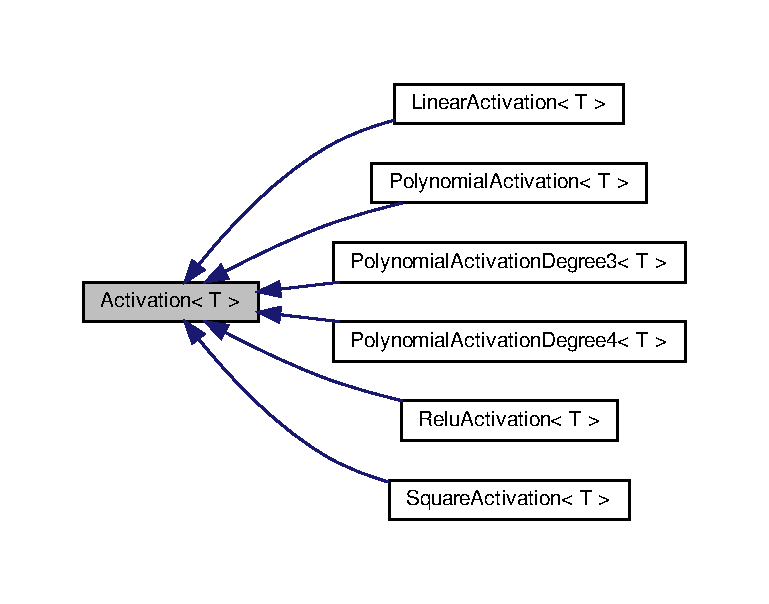
\includegraphics[width=350pt]{classActivation__inherit__graph}
\end{center}
\end{figure}
\subsection*{Public Member Functions}
\begin{DoxyCompactItemize}
\item 
\mbox{\Hypertarget{classActivation_aeffc71e7421ef3ff2b40550744a19af3}\label{classActivation_aeffc71e7421ef3ff2b40550744a19af3}} 
virtual void {\bfseries activate} (T \&in)=0
\end{DoxyCompactItemize}
\subsection*{Static Public Member Functions}
\begin{DoxyCompactItemize}
\item 
\mbox{\Hypertarget{classActivation_a20a28e39ac312019885e08f115fe2268}\label{classActivation_a20a28e39ac312019885e08f115fe2268}} 
static std\+::shared\+\_\+ptr$<$ \hyperlink{classActivation}{Activation}$<$ T $>$ $>$ {\bfseries get\+Shared\+Pointer} ()
\end{DoxyCompactItemize}


The documentation for this class was generated from the following file\+:\begin{DoxyCompactItemize}
\item 
src/architecture/Activation\+Function\+Impl.\+h\end{DoxyCompactItemize}

\hypertarget{structnlohmann_1_1adl__serializer}{}\section{nlohmann\+:\+:adl\+\_\+serializer$<$ typename, typename $>$ Struct Template Reference}
\label{structnlohmann_1_1adl__serializer}\index{nlohmann\+::adl\+\_\+serializer$<$ typename, typename $>$@{nlohmann\+::adl\+\_\+serializer$<$ typename, typename $>$}}


default J\+S\+O\+N\+Serializer template argument  




{\ttfamily \#include $<$json.\+hpp$>$}

\subsection*{Static Public Member Functions}
\begin{DoxyCompactItemize}
\item 
{\footnotesize template$<$typename Basic\+Json\+Type , typename Value\+Type $>$ }\\static auto \hyperlink{structnlohmann_1_1adl__serializer_a2c544585b8b1828a0f1eecd831d0496e}{from\+\_\+json} (Basic\+Json\+Type \&\&j, Value\+Type \&val) noexcept(noexcept(\+::nlohmann\+::from\+\_\+json(std\+::forward$<$ Basic\+Json\+Type $>$(j), val))) -\/$>$ decltype(\+::nlohmann\+::from\+\_\+json(std\+::forward$<$ Basic\+Json\+Type $>$(j), val), void())
\begin{DoxyCompactList}\small\item\em convert a J\+S\+ON value to any value type \end{DoxyCompactList}\item 
{\footnotesize template$<$typename Basic\+Json\+Type , typename Value\+Type $>$ }\\static auto \hyperlink{structnlohmann_1_1adl__serializer_a01b867bd5dce5249d4f7433b8f27def6}{to\+\_\+json} (Basic\+Json\+Type \&j, Value\+Type \&\&val) noexcept(noexcept(\+::nlohmann\+::to\+\_\+json(j, std\+::forward$<$ Value\+Type $>$(val)))) -\/$>$ decltype(\+::nlohmann\+::to\+\_\+json(j, std\+::forward$<$ Value\+Type $>$(val)), void())
\begin{DoxyCompactList}\small\item\em convert any value type to a J\+S\+ON value \end{DoxyCompactList}\end{DoxyCompactItemize}


\subsection{Detailed Description}
\subsubsection*{template$<$typename, typename$>$\newline
struct nlohmann\+::adl\+\_\+serializer$<$ typename, typename $>$}

default J\+S\+O\+N\+Serializer template argument 

This serializer ignores the template arguments and uses A\+DL (\href{https://en.cppreference.com/w/cpp/language/adl}{\tt argument-\/dependent lookup}) for serialization. 

\subsection{Member Function Documentation}
\mbox{\Hypertarget{structnlohmann_1_1adl__serializer_a2c544585b8b1828a0f1eecd831d0496e}\label{structnlohmann_1_1adl__serializer_a2c544585b8b1828a0f1eecd831d0496e}} 
\index{nlohmann\+::adl\+\_\+serializer@{nlohmann\+::adl\+\_\+serializer}!from\+\_\+json@{from\+\_\+json}}
\index{from\+\_\+json@{from\+\_\+json}!nlohmann\+::adl\+\_\+serializer@{nlohmann\+::adl\+\_\+serializer}}
\subsubsection{\texorpdfstring{from\+\_\+json()}{from\_json()}}
{\footnotesize\ttfamily template$<$typename , typename $>$ \\
template$<$typename Basic\+Json\+Type , typename Value\+Type $>$ \\
static auto \hyperlink{structnlohmann_1_1adl__serializer}{nlohmann\+::adl\+\_\+serializer}$<$ typename, typename $>$\+::from\+\_\+json (\begin{DoxyParamCaption}\item[{Basic\+Json\+Type \&\&}]{j,  }\item[{Value\+Type \&}]{val }\end{DoxyParamCaption}) -\/$>$ decltype(\+::nlohmann\+::from\+\_\+json(std\+::forward$<$Basic\+Json\+Type$>$(j), val), void())
    \hspace{0.3cm}{\ttfamily [inline]}, {\ttfamily [static]}, {\ttfamily [noexcept]}}



convert a J\+S\+ON value to any value type 

This function is usually called by the {\ttfamily get()} function of the \hyperlink{classnlohmann_1_1basic__json}{basic\+\_\+json} class (either explicit or via conversion operators).


\begin{DoxyParams}[1]{Parameters}
\mbox{\tt in}  & {\em j} & J\+S\+ON value to read from \\
\hline
\mbox{\tt in,out}  & {\em val} & value to write to \\
\hline
\end{DoxyParams}
\mbox{\Hypertarget{structnlohmann_1_1adl__serializer_a01b867bd5dce5249d4f7433b8f27def6}\label{structnlohmann_1_1adl__serializer_a01b867bd5dce5249d4f7433b8f27def6}} 
\index{nlohmann\+::adl\+\_\+serializer@{nlohmann\+::adl\+\_\+serializer}!to\+\_\+json@{to\+\_\+json}}
\index{to\+\_\+json@{to\+\_\+json}!nlohmann\+::adl\+\_\+serializer@{nlohmann\+::adl\+\_\+serializer}}
\subsubsection{\texorpdfstring{to\+\_\+json()}{to\_json()}}
{\footnotesize\ttfamily template$<$typename , typename $>$ \\
template$<$typename Basic\+Json\+Type , typename Value\+Type $>$ \\
static auto \hyperlink{structnlohmann_1_1adl__serializer}{nlohmann\+::adl\+\_\+serializer}$<$ typename, typename $>$\+::to\+\_\+json (\begin{DoxyParamCaption}\item[{Basic\+Json\+Type \&}]{j,  }\item[{Value\+Type \&\&}]{val }\end{DoxyParamCaption}) -\/$>$ decltype(\+::nlohmann\+::to\+\_\+json(j, std\+::forward$<$Value\+Type$>$(val)), void())
    \hspace{0.3cm}{\ttfamily [inline]}, {\ttfamily [static]}, {\ttfamily [noexcept]}}



convert any value type to a J\+S\+ON value 

This function is usually called by the constructors of the \hyperlink{classnlohmann_1_1basic__json}{basic\+\_\+json} class.


\begin{DoxyParams}[1]{Parameters}
\mbox{\tt in,out}  & {\em j} & J\+S\+ON value to write to \\
\hline
\mbox{\tt in}  & {\em val} & value to read from \\
\hline
\end{DoxyParams}


The documentation for this struct was generated from the following file\+:\begin{DoxyCompactItemize}
\item 
src/tools/json/json.\+hpp\end{DoxyCompactItemize}

\hypertarget{structTensor_1_1array__deleter}{}\section{Tensor$<$ Value\+Type $>$\+:\+:array\+\_\+deleter Struct Reference}
\label{structTensor_1_1array__deleter}\index{Tensor$<$ Value\+Type $>$\+::array\+\_\+deleter@{Tensor$<$ Value\+Type $>$\+::array\+\_\+deleter}}
\subsection*{Public Member Functions}
\begin{DoxyCompactItemize}
\item 
\mbox{\Hypertarget{structTensor_1_1array__deleter_aa01ba9dbcd93d3cdbec5ac354d10f3e7}\label{structTensor_1_1array__deleter_aa01ba9dbcd93d3cdbec5ac354d10f3e7}} 
void {\bfseries operator()} (Value\+Type const $\ast$p)
\end{DoxyCompactItemize}


The documentation for this struct was generated from the following file\+:\begin{DoxyCompactItemize}
\item 
src/architecture/Tensor\+Impl.\+h\end{DoxyCompactItemize}

\hypertarget{classAveragePooling}{}\section{Average\+Pooling$<$ Value\+Type, Weight\+Type, Data\+Tensor\+Type, Weight\+Tensor\+Type $>$ Class Template Reference}
\label{classAveragePooling}\index{Average\+Pooling$<$ Value\+Type, Weight\+Type, Data\+Tensor\+Type, Weight\+Tensor\+Type $>$@{Average\+Pooling$<$ Value\+Type, Weight\+Type, Data\+Tensor\+Type, Weight\+Tensor\+Type $>$}}


Inheritance diagram for Average\+Pooling$<$ Value\+Type, Weight\+Type, Data\+Tensor\+Type, Weight\+Tensor\+Type $>$\+:
\nopagebreak
\begin{figure}[H]
\begin{center}
\leavevmode
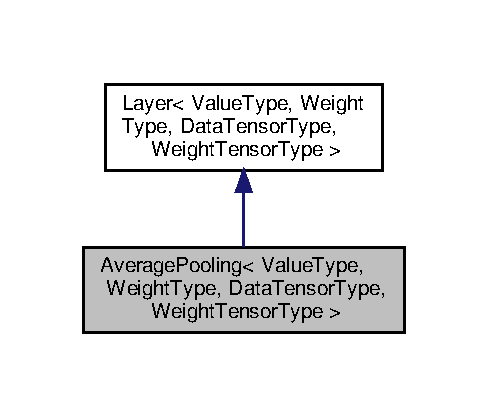
\includegraphics[width=234pt]{classAveragePooling__inherit__graph}
\end{center}
\end{figure}


Collaboration diagram for Average\+Pooling$<$ Value\+Type, Weight\+Type, Data\+Tensor\+Type, Weight\+Tensor\+Type $>$\+:
\nopagebreak
\begin{figure}[H]
\begin{center}
\leavevmode
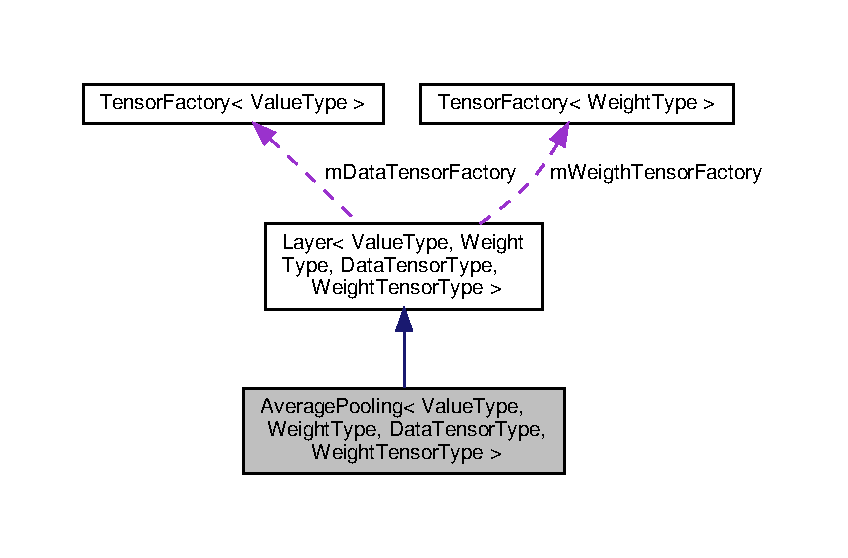
\includegraphics[width=350pt]{classAveragePooling__coll__graph}
\end{center}
\end{figure}
\subsection*{Public Member Functions}
\begin{DoxyCompactItemize}
\item 
\mbox{\Hypertarget{classAveragePooling_ad030f12eeea45648ad7044ec2781c1eb}\label{classAveragePooling_ad030f12eeea45648ad7044ec2781c1eb}} 
{\bfseries Average\+Pooling} (std\+::string name, ActivationP$<$ Value\+Type $>$ act, uint filter\+Size, uint stride, P\+A\+D\+D\+I\+N\+G\+\_\+\+M\+O\+DE pad, TensorP$<$ Value\+Type $>$ input, \hyperlink{classTensorFactory}{Tensor\+Factory}$<$ Value\+Type $>$ $\ast$data\+Tensor\+Factory, \hyperlink{classTensorFactory}{Tensor\+Factory}$<$ Weight\+Type $>$ $\ast$weigth\+Tensor\+Factory)
\item 
\mbox{\Hypertarget{classAveragePooling_a21550554dffab144ce43ef6c802567f0}\label{classAveragePooling_a21550554dffab144ce43ef6c802567f0}} 
{\bfseries Average\+Pooling} (std\+::string name, ActivationP$<$ Value\+Type $>$ act, uint filter\+Size, uint stride, P\+A\+D\+D\+I\+N\+G\+\_\+\+M\+O\+DE pad, \hyperlink{classTensorFactory}{Tensor\+Factory}$<$ Value\+Type $>$ $\ast$data\+Tensor\+Factory, \hyperlink{classTensorFactory}{Tensor\+Factory}$<$ Weight\+Type $>$ $\ast$weigth\+Tensor\+Factory)
\item 
\mbox{\Hypertarget{classAveragePooling_a6fda7d16c936b9dc81e0dd011c4b79ad}\label{classAveragePooling_a6fda7d16c936b9dc81e0dd011c4b79ad}} 
{\bfseries Average\+Pooling} (std\+::string name, ActivationP$<$ Value\+Type $>$ act, uint filter\+Size, uint stride, P\+A\+D\+D\+I\+N\+G\+\_\+\+M\+O\+DE pad, TensorP$<$ Value\+Type $>$ input)
\item 
\mbox{\Hypertarget{classAveragePooling_ac54cd5cc290db09b7b5ed6ad310a08aa}\label{classAveragePooling_ac54cd5cc290db09b7b5ed6ad310a08aa}} 
{\bfseries Average\+Pooling} (std\+::string name, ActivationP$<$ Value\+Type $>$ act, uint filter\+Size, uint stride, P\+A\+D\+D\+I\+N\+G\+\_\+\+M\+O\+DE pad)
\item 
\mbox{\Hypertarget{classAveragePooling_acd8ffd6531a30d85dfaf2d5f9afa602c}\label{classAveragePooling_acd8ffd6531a30d85dfaf2d5f9afa602c}} 
{\bfseries Average\+Pooling} (std\+::string name, uint filter\+Size, uint stride, P\+A\+D\+D\+I\+N\+G\+\_\+\+M\+O\+DE pad)
\item 
\mbox{\Hypertarget{classAveragePooling_ab7719a1498669eb0f3ee18149dddb30f}\label{classAveragePooling_ab7719a1498669eb0f3ee18149dddb30f}} 
{\bfseries Average\+Pooling} (std\+::string name, uint filter\+Size, uint stride, P\+A\+D\+D\+I\+N\+G\+\_\+\+M\+O\+DE pad, TensorP$<$ Value\+Type $>$ input)
\item 
\mbox{\Hypertarget{classAveragePooling_a17b7f49f29b6f6334cb023bd59fa5232}\label{classAveragePooling_a17b7f49f29b6f6334cb023bd59fa5232}} 
{\bfseries Average\+Pooling} (std\+::string name, ActivationP$<$ Value\+Type $>$ act, uint filter\+Size, uint stride, P\+A\+D\+D\+I\+N\+G\+\_\+\+M\+O\+DE pad, TensorP$<$ Value\+Type $>$ input, Tensor\+FactoryP$<$ Value\+Type $>$ data\+Tensor\+Factory, Tensor\+FactoryP$<$ Weight\+Type $>$ weight\+Tensor\+Factory)
\item 
\mbox{\Hypertarget{classAveragePooling_ae15db952116ae7491c789a4b9c2e91e2}\label{classAveragePooling_ae15db952116ae7491c789a4b9c2e91e2}} 
{\bfseries Average\+Pooling} (std\+::string name, ActivationP$<$ Value\+Type $>$ act, uint filter\+Size, uint stride, P\+A\+D\+D\+I\+N\+G\+\_\+\+M\+O\+DE pad, Tensor\+FactoryP$<$ Value\+Type $>$ data\+Tensor\+Factory, Tensor\+FactoryP$<$ Weight\+Type $>$ weight\+Tensor\+Factory)
\item 
\mbox{\Hypertarget{classAveragePooling_a12b3ae240455ee32a7fa0e567983efc6}\label{classAveragePooling_a12b3ae240455ee32a7fa0e567983efc6}} 
\hyperlink{classShape}{Shape} {\bfseries output\+Shape} () override
\item 
\mbox{\Hypertarget{classAveragePooling_a2111ac4ecad38c8d536a7c763ec2ad41}\label{classAveragePooling_a2111ac4ecad38c8d536a7c763ec2ad41}} 
void {\bfseries feed\+Forward} () override
\item 
\mbox{\Hypertarget{classAveragePooling_a7da9d260bae8a8d9f00ceb8b53939ab5}\label{classAveragePooling_a7da9d260bae8a8d9f00ceb8b53939ab5}} 
void {\bfseries load\+Weights} (std\+::string path, std\+::string file\+Name) override
\item 
\mbox{\Hypertarget{classAveragePooling_a4d8456525db187a9521c476b25ca41d9}\label{classAveragePooling_a4d8456525db187a9521c476b25ca41d9}} 
void {\bfseries load\+Weights} (std\+::string path) override
\item 
\mbox{\Hypertarget{classAveragePooling_ab115808921472b438c06b1408532e7c4}\label{classAveragePooling_ab115808921472b438c06b1408532e7c4}} 
void {\bfseries random\+Init} () override
\item 
\mbox{\Hypertarget{classAveragePooling_a51cae671de031a32d951846b34f21264}\label{classAveragePooling_a51cae671de031a32d951846b34f21264}} 
void {\bfseries description} () override
\item 
\mbox{\Hypertarget{classAveragePooling_a3db0eee227862f0c6c04f68da7d9d879}\label{classAveragePooling_a3db0eee227862f0c6c04f68da7d9d879}} 
virtual std\+::vector$<$ TensorP$<$ Weight\+Type $>$ $>$ \hyperlink{classAveragePooling_a3db0eee227862f0c6c04f68da7d9d879}{all\+Weights} () override
\begin{DoxyCompactList}\small\item\em Returns empyt vector. \end{DoxyCompactList}\end{DoxyCompactItemize}
\subsection*{Additional Inherited Members}


The documentation for this class was generated from the following file\+:\begin{DoxyCompactItemize}
\item 
src/architecture/Layer\+Impl.\+h\end{DoxyCompactItemize}

\hypertarget{classnlohmann_1_1basic__json}{}\section{nlohmann\+:\+:basic\+\_\+json$<$ Object\+Type, Array\+Type, String\+Type, Boolean\+Type, Number\+Integer\+Type, Number\+Unsigned\+Type, Number\+Float\+Type, Allocator\+Type, J\+S\+O\+N\+Serializer $>$ Class Template Reference}
\label{classnlohmann_1_1basic__json}\index{nlohmann\+::basic\+\_\+json$<$ Object\+Type, Array\+Type, String\+Type, Boolean\+Type, Number\+Integer\+Type, Number\+Unsigned\+Type, Number\+Float\+Type, Allocator\+Type, J\+S\+O\+N\+Serializer $>$@{nlohmann\+::basic\+\_\+json$<$ Object\+Type, Array\+Type, String\+Type, Boolean\+Type, Number\+Integer\+Type, Number\+Unsigned\+Type, Number\+Float\+Type, Allocator\+Type, J\+S\+O\+N\+Serializer $>$}}


a class to store J\+S\+ON values  




{\ttfamily \#include $<$json.\+hpp$>$}

\subsection*{Public Types}
\begin{DoxyCompactItemize}
\item 
\mbox{\Hypertarget{classnlohmann_1_1basic__json_ae8cbef097f7da18a781fc86587de6b90}\label{classnlohmann_1_1basic__json_ae8cbef097f7da18a781fc86587de6b90}} 
using {\bfseries value\+\_\+t} = \hyperlink{namespacenlohmann_1_1detail_a1ed8fc6239da25abcaf681d30ace4985}{detail\+::value\+\_\+t}
\item 
\mbox{\Hypertarget{classnlohmann_1_1basic__json_a6886a5001f5b449ad316101a311ce536}\label{classnlohmann_1_1basic__json_a6886a5001f5b449ad316101a311ce536}} 
using \hyperlink{classnlohmann_1_1basic__json_a6886a5001f5b449ad316101a311ce536}{json\+\_\+pointer} = \+::\hyperlink{classnlohmann_1_1json__pointer}{nlohmann\+::json\+\_\+pointer}$<$ \hyperlink{classnlohmann_1_1basic__json}{basic\+\_\+json} $>$
\begin{DoxyCompactList}\small\item\em J\+S\+ON Pointer, see \hyperlink{classnlohmann_1_1json__pointer}{nlohmann\+::json\+\_\+pointer}. \end{DoxyCompactList}\item 
\mbox{\Hypertarget{classnlohmann_1_1basic__json_a7768841baaaa7a21098a401c932efaff}\label{classnlohmann_1_1basic__json_a7768841baaaa7a21098a401c932efaff}} 
{\footnotesize template$<$typename T , typename S\+F\+I\+N\+AE $>$ }\\using {\bfseries json\+\_\+serializer} = J\+S\+O\+N\+Serializer$<$ T, S\+F\+I\+N\+AE $>$
\item 
\mbox{\Hypertarget{classnlohmann_1_1basic__json_ae56b6bfbb1f6d2f43611f2ada4f9e5f2}\label{classnlohmann_1_1basic__json_ae56b6bfbb1f6d2f43611f2ada4f9e5f2}} 
using \hyperlink{classnlohmann_1_1basic__json_ae56b6bfbb1f6d2f43611f2ada4f9e5f2}{error\+\_\+handler\+\_\+t} = \hyperlink{namespacenlohmann_1_1detail_a5a76b60b26dc8c47256a996d18d967df}{detail\+::error\+\_\+handler\+\_\+t}
\begin{DoxyCompactList}\small\item\em how to treat decoding errors \end{DoxyCompactList}\item 
\mbox{\Hypertarget{classnlohmann_1_1basic__json_ad70a098fbc01c53497db29d3b5b656a9}\label{classnlohmann_1_1basic__json_ad70a098fbc01c53497db29d3b5b656a9}} 
using \hyperlink{classnlohmann_1_1basic__json_ad70a098fbc01c53497db29d3b5b656a9}{initializer\+\_\+list\+\_\+t} = std\+::initializer\+\_\+list$<$ \hyperlink{classnlohmann_1_1detail_1_1json__ref}{detail\+::json\+\_\+ref}$<$ \hyperlink{classnlohmann_1_1basic__json}{basic\+\_\+json} $>$ $>$
\begin{DoxyCompactList}\small\item\em helper type for initializer lists of \hyperlink{classnlohmann_1_1basic__json}{basic\+\_\+json} values \end{DoxyCompactList}\item 
\mbox{\Hypertarget{classnlohmann_1_1basic__json_a2ddbac818a4c84a7377b1bbd25363588}\label{classnlohmann_1_1basic__json_a2ddbac818a4c84a7377b1bbd25363588}} 
using {\bfseries input\+\_\+format\+\_\+t} = \hyperlink{namespacenlohmann_1_1detail_aa554fc6a11519e4f347deb25a9f0db40}{detail\+::input\+\_\+format\+\_\+t}
\item 
\mbox{\Hypertarget{classnlohmann_1_1basic__json_aa865c3eb68b6ebdd647173774d2b5cdb}\label{classnlohmann_1_1basic__json_aa865c3eb68b6ebdd647173774d2b5cdb}} 
using \hyperlink{classnlohmann_1_1basic__json_aa865c3eb68b6ebdd647173774d2b5cdb}{json\+\_\+sax\+\_\+t} = \hyperlink{structnlohmann_1_1json__sax}{json\+\_\+sax}$<$ \hyperlink{classnlohmann_1_1basic__json}{basic\+\_\+json} $>$
\begin{DoxyCompactList}\small\item\em S\+AX interface type, see \hyperlink{structnlohmann_1_1json__sax}{nlohmann\+::json\+\_\+sax}. \end{DoxyCompactList}\item 
using \hyperlink{classnlohmann_1_1basic__json_aaceba2e4cf75fc983bb75c78c8742e65}{parse\+\_\+event\+\_\+t} = typename \hyperlink{classnlohmann_1_1detail_1_1parser_a37ac88c864dda495f72cb62776b0bebe}{parser\+::parse\+\_\+event\+\_\+t}
\begin{DoxyCompactList}\small\item\em parser event types \end{DoxyCompactList}\item 
using \hyperlink{classnlohmann_1_1basic__json_ab4f78c5f9fd25172eeec84482e03f5b7}{parser\+\_\+callback\+\_\+t} = typename parser\+::parser\+\_\+callback\+\_\+t
\begin{DoxyCompactList}\small\item\em per-\/element parser callback type \end{DoxyCompactList}\end{DoxyCompactItemize}
\subsection*{Public Member Functions}
\begin{DoxyCompactItemize}
\item 
const char $\ast$ \hyperlink{classnlohmann_1_1basic__json_a9d0a478571f82f0163b96b2424cd998f}{type\+\_\+name} () const noexcept
\begin{DoxyCompactList}\small\item\em return the type as string \end{DoxyCompactList}\end{DoxyCompactItemize}
\subsection*{Static Public Member Functions}
\begin{DoxyCompactItemize}
\item 
\mbox{\Hypertarget{classnlohmann_1_1basic__json_af4ac14224fbdd29d3547fcb11bb55c8f}\label{classnlohmann_1_1basic__json_af4ac14224fbdd29d3547fcb11bb55c8f}} 
static \hyperlink{classnlohmann_1_1basic__json_a86ce930490cf7773b26f5ef49c04a350}{allocator\+\_\+type} \hyperlink{classnlohmann_1_1basic__json_af4ac14224fbdd29d3547fcb11bb55c8f}{get\+\_\+allocator} ()
\begin{DoxyCompactList}\small\item\em returns the allocator associated with the container \end{DoxyCompactList}\item 
static J\+S\+O\+N\+\_\+\+N\+O\+D\+I\+S\+C\+A\+RD \hyperlink{classnlohmann_1_1basic__json}{basic\+\_\+json} \hyperlink{classnlohmann_1_1basic__json_a563810575fe32eed55aa5355f6bdc4a7}{meta} ()
\begin{DoxyCompactList}\small\item\em returns version information on the library \end{DoxyCompactList}\end{DoxyCompactItemize}
\subsection*{Friends}
\begin{DoxyCompactItemize}
\item 
\mbox{\Hypertarget{classnlohmann_1_1basic__json_a6275ed57bae6866cdf5db5370a7ad47c}\label{classnlohmann_1_1basic__json_a6275ed57bae6866cdf5db5370a7ad47c}} 
{\footnotesize template$<$detail\+::value\+\_\+t $>$ }\\struct {\bfseries detail\+::external\+\_\+constructor}
\item 
\mbox{\Hypertarget{classnlohmann_1_1basic__json_a842e5c7ca096025c18b11e715d3401f4}\label{classnlohmann_1_1basic__json_a842e5c7ca096025c18b11e715d3401f4}} 
{\footnotesize template$<$typename Basic\+Json\+Type $>$ }\\class {\bfseries \+::nlohmann\+::detail\+::iter\+\_\+impl}
\item 
\mbox{\Hypertarget{classnlohmann_1_1basic__json_a69d491bbda88ade6d3c7a2b11309e8bf}\label{classnlohmann_1_1basic__json_a69d491bbda88ade6d3c7a2b11309e8bf}} 
{\footnotesize template$<$typename Basic\+Json\+Type , typename Char\+Type $>$ }\\class {\bfseries \+::nlohmann\+::detail\+::binary\+\_\+writer}
\item 
\mbox{\Hypertarget{classnlohmann_1_1basic__json_a3226693341c251507fec5d6f4fa5ce79}\label{classnlohmann_1_1basic__json_a3226693341c251507fec5d6f4fa5ce79}} 
{\footnotesize template$<$typename Basic\+Json\+Type , typename S\+AX $>$ }\\class {\bfseries \+::nlohmann\+::detail\+::binary\+\_\+reader}
\item 
\mbox{\Hypertarget{classnlohmann_1_1basic__json_a47aabb1eceae32e8a6e8e7f0ff34be60}\label{classnlohmann_1_1basic__json_a47aabb1eceae32e8a6e8e7f0ff34be60}} 
{\footnotesize template$<$typename Basic\+Json\+Type $>$ }\\class {\bfseries \+::nlohmann\+::detail\+::json\+\_\+sax\+\_\+dom\+\_\+parser}
\item 
\mbox{\Hypertarget{classnlohmann_1_1basic__json_a95574da8d12905ea99dc348934c837da}\label{classnlohmann_1_1basic__json_a95574da8d12905ea99dc348934c837da}} 
{\footnotesize template$<$typename Basic\+Json\+Type $>$ }\\class {\bfseries \+::nlohmann\+::detail\+::json\+\_\+sax\+\_\+dom\+\_\+callback\+\_\+parser}
\end{DoxyCompactItemize}
\subsection*{exceptions}
\label{_amgrp19ad27801b95bd1f2c6c2bf83dbb7515}%
Classes to implement user-\/defined exceptions. \begin{DoxyCompactItemize}
\item 
using \hyperlink{classnlohmann_1_1basic__json_a9a0aced019cb1d65bb49703406c84970}{exception} = \hyperlink{classnlohmann_1_1detail_1_1exception}{detail\+::exception}
\begin{DoxyCompactList}\small\item\em general exception of the \hyperlink{classnlohmann_1_1basic__json}{basic\+\_\+json} class \end{DoxyCompactList}\item 
using \hyperlink{classnlohmann_1_1basic__json_af1efc2468e6022be6e35fc2944cabe4d}{parse\+\_\+error} = \hyperlink{classnlohmann_1_1detail_1_1parse__error}{detail\+::parse\+\_\+error}
\begin{DoxyCompactList}\small\item\em exception indicating a parse error \end{DoxyCompactList}\item 
using \hyperlink{classnlohmann_1_1basic__json_ac13d32f7cbd02d616e71d8dc30dadcbf}{invalid\+\_\+iterator} = \hyperlink{classnlohmann_1_1detail_1_1invalid__iterator}{detail\+::invalid\+\_\+iterator}
\begin{DoxyCompactList}\small\item\em exception indicating errors with iterators \end{DoxyCompactList}\item 
using \hyperlink{classnlohmann_1_1basic__json_a4010e8e268fefd86da773c10318f2902}{type\+\_\+error} = \hyperlink{classnlohmann_1_1detail_1_1type__error}{detail\+::type\+\_\+error}
\begin{DoxyCompactList}\small\item\em exception indicating executing a member function with a wrong type \end{DoxyCompactList}\item 
using \hyperlink{classnlohmann_1_1basic__json_a28f7c2f087274a0012eb7a2333ee1580}{out\+\_\+of\+\_\+range} = \hyperlink{classnlohmann_1_1detail_1_1out__of__range}{detail\+::out\+\_\+of\+\_\+range}
\begin{DoxyCompactList}\small\item\em exception indicating access out of the defined range \end{DoxyCompactList}\item 
using \hyperlink{classnlohmann_1_1basic__json_a3333a5a8714912adda33a35b369f7b3d}{other\+\_\+error} = \hyperlink{classnlohmann_1_1detail_1_1other__error}{detail\+::other\+\_\+error}
\begin{DoxyCompactList}\small\item\em exception indicating other library errors \end{DoxyCompactList}\end{DoxyCompactItemize}
\subsection*{container types}
\label{_amgrp6618fa684bc6d5a05e2c88bfff1c0d66}%
The canonic container types to use \hyperlink{classnlohmann_1_1basic__json}{basic\+\_\+json} like any other S\+TL container. \begin{DoxyCompactItemize}
\item 
\mbox{\Hypertarget{classnlohmann_1_1basic__json_a2b3297873b70c080837e8eedc4fec32f}\label{classnlohmann_1_1basic__json_a2b3297873b70c080837e8eedc4fec32f}} 
using \hyperlink{classnlohmann_1_1basic__json_a2b3297873b70c080837e8eedc4fec32f}{value\+\_\+type} = \hyperlink{classnlohmann_1_1basic__json}{basic\+\_\+json}
\begin{DoxyCompactList}\small\item\em the type of elements in a \hyperlink{classnlohmann_1_1basic__json}{basic\+\_\+json} container \end{DoxyCompactList}\item 
\mbox{\Hypertarget{classnlohmann_1_1basic__json_ac6a5eddd156c776ac75ff54cfe54a5bc}\label{classnlohmann_1_1basic__json_ac6a5eddd156c776ac75ff54cfe54a5bc}} 
using \hyperlink{classnlohmann_1_1basic__json_ac6a5eddd156c776ac75ff54cfe54a5bc}{reference} = \hyperlink{classnlohmann_1_1basic__json_a2b3297873b70c080837e8eedc4fec32f}{value\+\_\+type} \&
\begin{DoxyCompactList}\small\item\em the type of an element reference \end{DoxyCompactList}\item 
\mbox{\Hypertarget{classnlohmann_1_1basic__json_a4057c5425f4faacfe39a8046871786ca}\label{classnlohmann_1_1basic__json_a4057c5425f4faacfe39a8046871786ca}} 
using \hyperlink{classnlohmann_1_1basic__json_a4057c5425f4faacfe39a8046871786ca}{const\+\_\+reference} = const \hyperlink{classnlohmann_1_1basic__json_a2b3297873b70c080837e8eedc4fec32f}{value\+\_\+type} \&
\begin{DoxyCompactList}\small\item\em the type of an element const reference \end{DoxyCompactList}\item 
\mbox{\Hypertarget{classnlohmann_1_1basic__json_afe7c1303357e19cea9527af4e9a31d8f}\label{classnlohmann_1_1basic__json_afe7c1303357e19cea9527af4e9a31d8f}} 
using \hyperlink{classnlohmann_1_1basic__json_afe7c1303357e19cea9527af4e9a31d8f}{difference\+\_\+type} = std\+::ptrdiff\+\_\+t
\begin{DoxyCompactList}\small\item\em a type to represent differences between iterators \end{DoxyCompactList}\item 
\mbox{\Hypertarget{classnlohmann_1_1basic__json_a39f2cd0b58106097e0e67bf185cc519b}\label{classnlohmann_1_1basic__json_a39f2cd0b58106097e0e67bf185cc519b}} 
using \hyperlink{classnlohmann_1_1basic__json_a39f2cd0b58106097e0e67bf185cc519b}{size\+\_\+type} = std\+::size\+\_\+t
\begin{DoxyCompactList}\small\item\em a type to represent container sizes \end{DoxyCompactList}\item 
\mbox{\Hypertarget{classnlohmann_1_1basic__json_a86ce930490cf7773b26f5ef49c04a350}\label{classnlohmann_1_1basic__json_a86ce930490cf7773b26f5ef49c04a350}} 
using \hyperlink{classnlohmann_1_1basic__json_a86ce930490cf7773b26f5ef49c04a350}{allocator\+\_\+type} = Allocator\+Type$<$ \hyperlink{classnlohmann_1_1basic__json}{basic\+\_\+json} $>$
\begin{DoxyCompactList}\small\item\em the allocator type \end{DoxyCompactList}\item 
\mbox{\Hypertarget{classnlohmann_1_1basic__json_aefee1f777198c68724bd127e0c8abbe4}\label{classnlohmann_1_1basic__json_aefee1f777198c68724bd127e0c8abbe4}} 
using \hyperlink{classnlohmann_1_1basic__json_aefee1f777198c68724bd127e0c8abbe4}{pointer} = typename std\+::allocator\+\_\+traits$<$ \hyperlink{classnlohmann_1_1basic__json_a86ce930490cf7773b26f5ef49c04a350}{allocator\+\_\+type} $>$\+::\hyperlink{classnlohmann_1_1basic__json_aefee1f777198c68724bd127e0c8abbe4}{pointer}
\begin{DoxyCompactList}\small\item\em the type of an element pointer \end{DoxyCompactList}\item 
\mbox{\Hypertarget{classnlohmann_1_1basic__json_aff3d5cd2a75612364b888d8693231b58}\label{classnlohmann_1_1basic__json_aff3d5cd2a75612364b888d8693231b58}} 
using \hyperlink{classnlohmann_1_1basic__json_aff3d5cd2a75612364b888d8693231b58}{const\+\_\+pointer} = typename std\+::allocator\+\_\+traits$<$ \hyperlink{classnlohmann_1_1basic__json_a86ce930490cf7773b26f5ef49c04a350}{allocator\+\_\+type} $>$\+::\hyperlink{classnlohmann_1_1basic__json_aff3d5cd2a75612364b888d8693231b58}{const\+\_\+pointer}
\begin{DoxyCompactList}\small\item\em the type of an element const pointer \end{DoxyCompactList}\item 
\mbox{\Hypertarget{classnlohmann_1_1basic__json_a099316232c76c034030a38faa6e34dca}\label{classnlohmann_1_1basic__json_a099316232c76c034030a38faa6e34dca}} 
using \hyperlink{classnlohmann_1_1basic__json_a099316232c76c034030a38faa6e34dca}{iterator} = \hyperlink{classnlohmann_1_1detail_1_1iter__impl}{iter\+\_\+impl}$<$ \hyperlink{classnlohmann_1_1basic__json}{basic\+\_\+json} $>$
\begin{DoxyCompactList}\small\item\em an iterator for a \hyperlink{classnlohmann_1_1basic__json}{basic\+\_\+json} container \end{DoxyCompactList}\item 
\mbox{\Hypertarget{classnlohmann_1_1basic__json_a41a70cf9993951836d129bb1c2b3126a}\label{classnlohmann_1_1basic__json_a41a70cf9993951836d129bb1c2b3126a}} 
using \hyperlink{classnlohmann_1_1basic__json_a41a70cf9993951836d129bb1c2b3126a}{const\+\_\+iterator} = \hyperlink{classnlohmann_1_1detail_1_1iter__impl}{iter\+\_\+impl}$<$ const \hyperlink{classnlohmann_1_1basic__json}{basic\+\_\+json} $>$
\begin{DoxyCompactList}\small\item\em a const iterator for a \hyperlink{classnlohmann_1_1basic__json}{basic\+\_\+json} container \end{DoxyCompactList}\item 
\mbox{\Hypertarget{classnlohmann_1_1basic__json_ac223d5560c2b05a208c88de67376c5f2}\label{classnlohmann_1_1basic__json_ac223d5560c2b05a208c88de67376c5f2}} 
using \hyperlink{classnlohmann_1_1basic__json_ac223d5560c2b05a208c88de67376c5f2}{reverse\+\_\+iterator} = \hyperlink{classnlohmann_1_1detail_1_1json__reverse__iterator}{json\+\_\+reverse\+\_\+iterator}$<$ typename \hyperlink{classnlohmann_1_1basic__json_a099316232c76c034030a38faa6e34dca}{basic\+\_\+json\+::iterator} $>$
\begin{DoxyCompactList}\small\item\em a reverse iterator for a \hyperlink{classnlohmann_1_1basic__json}{basic\+\_\+json} container \end{DoxyCompactList}\item 
\mbox{\Hypertarget{classnlohmann_1_1basic__json_a72be3c24bfa24f0993d6c11af03e7404}\label{classnlohmann_1_1basic__json_a72be3c24bfa24f0993d6c11af03e7404}} 
using \hyperlink{classnlohmann_1_1basic__json_a72be3c24bfa24f0993d6c11af03e7404}{const\+\_\+reverse\+\_\+iterator} = \hyperlink{classnlohmann_1_1detail_1_1json__reverse__iterator}{json\+\_\+reverse\+\_\+iterator}$<$ typename \hyperlink{classnlohmann_1_1basic__json_a41a70cf9993951836d129bb1c2b3126a}{basic\+\_\+json\+::const\+\_\+iterator} $>$
\begin{DoxyCompactList}\small\item\em a const reverse iterator for a \hyperlink{classnlohmann_1_1basic__json}{basic\+\_\+json} container \end{DoxyCompactList}\end{DoxyCompactItemize}
\subsection*{J\+S\+ON value data types}
\label{_amgrpbddfba6d49869d59bfd397e65b8cba87}%
The data types to store a J\+S\+ON value. These types are derived from the template arguments passed to class \hyperlink{classnlohmann_1_1basic__json}{basic\+\_\+json}. \begin{DoxyCompactItemize}
\item 
\mbox{\Hypertarget{classnlohmann_1_1basic__json_abed9e77c5fcfc925fcdd489911069c3b}\label{classnlohmann_1_1basic__json_abed9e77c5fcfc925fcdd489911069c3b}} 
using {\bfseries object\+\_\+comparator\+\_\+t} = std\+::less$<$ String\+Type $>$
\item 
using \hyperlink{classnlohmann_1_1basic__json_a5e48a7893520e1314bf0c9723e26ea2a}{object\+\_\+t} = Object\+Type$<$ String\+Type, \hyperlink{classnlohmann_1_1basic__json}{basic\+\_\+json}, object\+\_\+comparator\+\_\+t, Allocator\+Type$<$ std\+::pair$<$ const String\+Type, \hyperlink{classnlohmann_1_1basic__json}{basic\+\_\+json} $>$ $>$$>$
\begin{DoxyCompactList}\small\item\em a type for an object \end{DoxyCompactList}\item 
using \hyperlink{classnlohmann_1_1basic__json_ae095578e03df97c5b3991787f1056374}{array\+\_\+t} = Array\+Type$<$ \hyperlink{classnlohmann_1_1basic__json}{basic\+\_\+json}, Allocator\+Type$<$ \hyperlink{classnlohmann_1_1basic__json}{basic\+\_\+json} $>$ $>$
\begin{DoxyCompactList}\small\item\em a type for an array \end{DoxyCompactList}\item 
using \hyperlink{classnlohmann_1_1basic__json_a61f8566a1a85a424c7266fb531dca005}{string\+\_\+t} = String\+Type
\begin{DoxyCompactList}\small\item\em a type for a string \end{DoxyCompactList}\item 
using \hyperlink{classnlohmann_1_1basic__json_a4c919102a9b4fe0d588af64801436082}{boolean\+\_\+t} = Boolean\+Type
\begin{DoxyCompactList}\small\item\em a type for a boolean \end{DoxyCompactList}\item 
using \hyperlink{classnlohmann_1_1basic__json_a98e611d67b7bd75307de99c9358ab2dc}{number\+\_\+integer\+\_\+t} = Number\+Integer\+Type
\begin{DoxyCompactList}\small\item\em a type for a number (integer) \end{DoxyCompactList}\item 
using \hyperlink{classnlohmann_1_1basic__json_ab906e29b5d83ac162e823ada2156b989}{number\+\_\+unsigned\+\_\+t} = Number\+Unsigned\+Type
\begin{DoxyCompactList}\small\item\em a type for a number (unsigned) \end{DoxyCompactList}\item 
using \hyperlink{classnlohmann_1_1basic__json_a88d6103cb3620410b35200ee8e313d97}{number\+\_\+float\+\_\+t} = Number\+Float\+Type
\begin{DoxyCompactList}\small\item\em a type for a number (floating-\/point) \end{DoxyCompactList}\end{DoxyCompactItemize}
\subsection*{constructors and destructors}
\label{_amgrpd94b4d3d0135946bb7bdf25e48755337}%
Constructors of class \hyperlink{classnlohmann_1_1basic__json}{basic\+\_\+json}, copy/move constructor, copy assignment, static functions creating objects, and the destructor. \begin{DoxyCompactItemize}
\item 
static J\+S\+O\+N\+\_\+\+N\+O\+D\+I\+S\+C\+A\+RD \hyperlink{classnlohmann_1_1basic__json}{basic\+\_\+json} \hyperlink{classnlohmann_1_1basic__json_a9ad7ec0bc1082ed09d10900fbb20a21f}{array} (\hyperlink{classnlohmann_1_1basic__json_ad70a098fbc01c53497db29d3b5b656a9}{initializer\+\_\+list\+\_\+t} init=\{\})
\begin{DoxyCompactList}\small\item\em explicitly create an array from an initializer list \end{DoxyCompactList}\item 
static J\+S\+O\+N\+\_\+\+N\+O\+D\+I\+S\+C\+A\+RD \hyperlink{classnlohmann_1_1basic__json}{basic\+\_\+json} \hyperlink{classnlohmann_1_1basic__json_aaf509a7c029100d292187068f61c99b8}{object} (\hyperlink{classnlohmann_1_1basic__json_ad70a098fbc01c53497db29d3b5b656a9}{initializer\+\_\+list\+\_\+t} init=\{\})
\begin{DoxyCompactList}\small\item\em explicitly create an object from an initializer list \end{DoxyCompactList}\item 
\hyperlink{classnlohmann_1_1basic__json_aed115142bd0c6c66c864700e0467df55}{basic\+\_\+json} (const \hyperlink{namespacenlohmann_1_1detail_a1ed8fc6239da25abcaf681d30ace4985}{value\+\_\+t} v)
\begin{DoxyCompactList}\small\item\em create an empty value with a given type \end{DoxyCompactList}\item 
\hyperlink{classnlohmann_1_1basic__json_ae9be9e956bfc4658f35d17c6aa72b063}{basic\+\_\+json} (std\+::nullptr\+\_\+t=nullptr) noexcept
\begin{DoxyCompactList}\small\item\em create a null object \end{DoxyCompactList}\item 
{\footnotesize template$<$typename Compatible\+Type , typename U  = detail\+::uncvref\+\_\+t$<$\+Compatible\+Type$>$, detail\+::enable\+\_\+if\+\_\+t$<$ not detail\+::is\+\_\+basic\+\_\+json$<$ U $>$\+::value and detail\+::is\+\_\+compatible\+\_\+type$<$ basic\+\_\+json\+\_\+t, U $>$\+::value, int $>$  = 0$>$ }\\\hyperlink{classnlohmann_1_1basic__json_a5a6558bfd1be139a638f91f0e09fc737}{basic\+\_\+json} (Compatible\+Type \&\&val) noexcept(noexcept(J\+S\+O\+N\+Serializer$<$ U $>$\+::to\+\_\+json(std\+::declval$<$ basic\+\_\+json\+\_\+t \&$>$(), std\+::forward$<$ Compatible\+Type $>$(val))))
\begin{DoxyCompactList}\small\item\em create a J\+S\+ON value \end{DoxyCompactList}\item 
{\footnotesize template$<$typename Basic\+Json\+Type , detail\+::enable\+\_\+if\+\_\+t$<$ detail\+::is\+\_\+basic\+\_\+json$<$ Basic\+Json\+Type $>$\+::value and not std\+::is\+\_\+same$<$ basic\+\_\+json, Basic\+Json\+Type $>$\+::value, int $>$  = 0$>$ }\\\hyperlink{classnlohmann_1_1basic__json_aa16dc469c842fa8a0aaf6f5a95c46bb3}{basic\+\_\+json} (const Basic\+Json\+Type \&val)
\begin{DoxyCompactList}\small\item\em create a J\+S\+ON value from an existing one \end{DoxyCompactList}\item 
\hyperlink{classnlohmann_1_1basic__json_ab5dfd9a2b2663b219641cb7fe59b6da2}{basic\+\_\+json} (\hyperlink{classnlohmann_1_1basic__json_ad70a098fbc01c53497db29d3b5b656a9}{initializer\+\_\+list\+\_\+t} init, bool type\+\_\+deduction=true, \hyperlink{namespacenlohmann_1_1detail_a1ed8fc6239da25abcaf681d30ace4985}{value\+\_\+t} manual\+\_\+type=\hyperlink{namespacenlohmann_1_1detail_a1ed8fc6239da25abcaf681d30ace4985af1f713c9e000f5d3f280adbd124df4f5}{value\+\_\+t\+::array})
\begin{DoxyCompactList}\small\item\em create a container (array or object) from an initializer list \end{DoxyCompactList}\item 
\hyperlink{classnlohmann_1_1basic__json_ab6816ae5100409254ed0a8bc21c387bb}{basic\+\_\+json} (\hyperlink{classnlohmann_1_1basic__json_a39f2cd0b58106097e0e67bf185cc519b}{size\+\_\+type} cnt, const \hyperlink{classnlohmann_1_1basic__json}{basic\+\_\+json} \&val)
\begin{DoxyCompactList}\small\item\em construct an array with count copies of given value \end{DoxyCompactList}\item 
{\footnotesize template$<$class Input\+IT , typename std\+::enable\+\_\+if$<$ std\+::is\+\_\+same$<$ Input\+I\+T, typename basic\+\_\+json\+\_\+t\+::iterator $>$\+::value or std\+::is\+\_\+same$<$ Input\+I\+T, typename basic\+\_\+json\+\_\+t\+::const\+\_\+iterator $>$\+::value, int $>$\+::type  = 0$>$ }\\\hyperlink{classnlohmann_1_1basic__json_abe197e9f3184487805cfb5bba6fd5938}{basic\+\_\+json} (Input\+IT first, Input\+IT last)
\begin{DoxyCompactList}\small\item\em construct a J\+S\+ON container given an iterator range \end{DoxyCompactList}\item 
\hyperlink{classnlohmann_1_1basic__json_af5de621bcf646c332343f9c1e011126c}{basic\+\_\+json} (const \hyperlink{classnlohmann_1_1basic__json}{basic\+\_\+json} \&other)
\begin{DoxyCompactList}\small\item\em copy constructor \end{DoxyCompactList}\item 
\hyperlink{classnlohmann_1_1basic__json_a9a06d1efd50a00f4889f831f851ce124}{basic\+\_\+json} (\hyperlink{classnlohmann_1_1basic__json}{basic\+\_\+json} \&\&other) noexcept
\begin{DoxyCompactList}\small\item\em move constructor \end{DoxyCompactList}\item 
\hyperlink{classnlohmann_1_1basic__json}{basic\+\_\+json} \& \hyperlink{classnlohmann_1_1basic__json_a849368ca71af3a93d576939d486f61c7}{operator=} (\hyperlink{classnlohmann_1_1basic__json}{basic\+\_\+json} other) noexcept(std\+::is\+\_\+nothrow\+\_\+move\+\_\+constructible$<$ \hyperlink{namespacenlohmann_1_1detail_a1ed8fc6239da25abcaf681d30ace4985}{value\+\_\+t} $>$\+::\hyperlink{classnlohmann_1_1basic__json_adcf8ca5079f5db993820bf50036bf45d}{value} and std\+::is\+\_\+nothrow\+\_\+move\+\_\+assignable$<$ \hyperlink{namespacenlohmann_1_1detail_a1ed8fc6239da25abcaf681d30ace4985}{value\+\_\+t} $>$\+::\hyperlink{classnlohmann_1_1basic__json_adcf8ca5079f5db993820bf50036bf45d}{value} and std\+::is\+\_\+nothrow\+\_\+move\+\_\+constructible$<$ json\+\_\+value $>$\+::\hyperlink{classnlohmann_1_1basic__json_adcf8ca5079f5db993820bf50036bf45d}{value} and std\+::is\+\_\+nothrow\+\_\+move\+\_\+assignable$<$ json\+\_\+value $>$\+::\hyperlink{classnlohmann_1_1basic__json_adcf8ca5079f5db993820bf50036bf45d}{value})
\begin{DoxyCompactList}\small\item\em copy assignment \end{DoxyCompactList}\item 
\hyperlink{classnlohmann_1_1basic__json_aba01953d5d90e676d504863b8d9fdde5}{$\sim$basic\+\_\+json} () noexcept
\begin{DoxyCompactList}\small\item\em destructor \end{DoxyCompactList}\end{DoxyCompactItemize}
\subsection*{object inspection}
\label{_amgrpbbb01a37b8f261ae5b5799058dcac1a0}%
Functions to inspect the type of a J\+S\+ON value. \begin{DoxyCompactItemize}
\item 
\hyperlink{classnlohmann_1_1basic__json_a61f8566a1a85a424c7266fb531dca005}{string\+\_\+t} \hyperlink{classnlohmann_1_1basic__json_a50ec80b02d0f3f51130d4abb5d1cfdc5}{dump} (const int indent=-\/1, const char indent\+\_\+char=\textquotesingle{} \textquotesingle{}, const bool ensure\+\_\+ascii=false, const \hyperlink{namespacenlohmann_1_1detail_a5a76b60b26dc8c47256a996d18d967df}{error\+\_\+handler\+\_\+t} error\+\_\+handler=error\+\_\+handler\+\_\+t\+::strict) const
\begin{DoxyCompactList}\small\item\em serialization \end{DoxyCompactList}\item 
constexpr \hyperlink{namespacenlohmann_1_1detail_a1ed8fc6239da25abcaf681d30ace4985}{value\+\_\+t} \hyperlink{classnlohmann_1_1basic__json_a2b2d781d7f2a4ee41bc0016e931cadf7}{type} () const noexcept
\begin{DoxyCompactList}\small\item\em return the type of the J\+S\+ON value (explicit) \end{DoxyCompactList}\item 
constexpr bool \hyperlink{classnlohmann_1_1basic__json_a6362b88718eb5c6d4fed6a61eed44b95}{is\+\_\+primitive} () const noexcept
\begin{DoxyCompactList}\small\item\em return whether type is primitive \end{DoxyCompactList}\item 
constexpr bool \hyperlink{classnlohmann_1_1basic__json_a9f68a0af820c3ced7f9d17851ce4c22d}{is\+\_\+structured} () const noexcept
\begin{DoxyCompactList}\small\item\em return whether type is structured \end{DoxyCompactList}\item 
constexpr bool \hyperlink{classnlohmann_1_1basic__json_a8faa039ca82427ed29c486ffd00600c3}{is\+\_\+null} () const noexcept
\begin{DoxyCompactList}\small\item\em return whether value is null \end{DoxyCompactList}\item 
constexpr bool \hyperlink{classnlohmann_1_1basic__json_a943e8cb182d0f2365c76d64b42eaa6fd}{is\+\_\+boolean} () const noexcept
\begin{DoxyCompactList}\small\item\em return whether value is a boolean \end{DoxyCompactList}\item 
constexpr bool \hyperlink{classnlohmann_1_1basic__json_a2b9852390abb4b1ef5fac6984e2fc0f3}{is\+\_\+number} () const noexcept
\begin{DoxyCompactList}\small\item\em return whether value is a number \end{DoxyCompactList}\item 
constexpr bool \hyperlink{classnlohmann_1_1basic__json_abac8af76067f1e8fdca9052882c74428}{is\+\_\+number\+\_\+integer} () const noexcept
\begin{DoxyCompactList}\small\item\em return whether value is an integer number \end{DoxyCompactList}\item 
constexpr bool \hyperlink{classnlohmann_1_1basic__json_abc7378cba0613a78b9aad1c8e7044bb0}{is\+\_\+number\+\_\+unsigned} () const noexcept
\begin{DoxyCompactList}\small\item\em return whether value is an unsigned integer number \end{DoxyCompactList}\item 
constexpr bool \hyperlink{classnlohmann_1_1basic__json_a33b4bf898b857c962e798fc7f6e86e70}{is\+\_\+number\+\_\+float} () const noexcept
\begin{DoxyCompactList}\small\item\em return whether value is a floating-\/point number \end{DoxyCompactList}\item 
constexpr bool \hyperlink{classnlohmann_1_1basic__json_af8f511af124e82e4579f444b4175787c}{is\+\_\+object} () const noexcept
\begin{DoxyCompactList}\small\item\em return whether value is an object \end{DoxyCompactList}\item 
constexpr bool \hyperlink{classnlohmann_1_1basic__json_aef9ce5dd2381caee1f8ddcdb5bdd9c65}{is\+\_\+array} () const noexcept
\begin{DoxyCompactList}\small\item\em return whether value is an array \end{DoxyCompactList}\item 
constexpr bool \hyperlink{classnlohmann_1_1basic__json_a69b596a4a6683b362095c9a139637396}{is\+\_\+string} () const noexcept
\begin{DoxyCompactList}\small\item\em return whether value is a string \end{DoxyCompactList}\item 
constexpr bool \hyperlink{classnlohmann_1_1basic__json_aabe623bc8304c2ba92d96d91f390fab4}{is\+\_\+discarded} () const noexcept
\begin{DoxyCompactList}\small\item\em return whether value is discarded \end{DoxyCompactList}\item 
constexpr \hyperlink{classnlohmann_1_1basic__json_a26ef3058e249f82a04f8ec18f7419027}{operator value\+\_\+t} () const noexcept
\begin{DoxyCompactList}\small\item\em return the type of the J\+S\+ON value (implicit) \end{DoxyCompactList}\end{DoxyCompactItemize}
\subsection*{value access}
\label{_amgrpd8f53c9caf18314e5b3f758245606995}%
Direct access to the stored value of a J\+S\+ON value. \begin{DoxyCompactItemize}
\item 
{\footnotesize template$<$typename Basic\+Json\+Type , detail\+::enable\+\_\+if\+\_\+t$<$ std\+::is\+\_\+same$<$ typename std\+::remove\+\_\+const$<$ Basic\+Json\+Type $>$\+::type, basic\+\_\+json\+\_\+t $>$\+::value, int $>$  = 0$>$ }\\\hyperlink{classnlohmann_1_1basic__json}{basic\+\_\+json} \hyperlink{classnlohmann_1_1basic__json_a6b187a22994c12c8cae0dd5ee99dc85e}{get} () const
\begin{DoxyCompactList}\small\item\em get special-\/case overload \end{DoxyCompactList}\item 
{\footnotesize template$<$typename Basic\+Json\+Type , detail\+::enable\+\_\+if\+\_\+t$<$ not std\+::is\+\_\+same$<$ Basic\+Json\+Type, basic\+\_\+json $>$\+::value and detail\+::is\+\_\+basic\+\_\+json$<$ Basic\+Json\+Type $>$\+::value, int $>$  = 0$>$ }\\Basic\+Json\+Type \hyperlink{classnlohmann_1_1basic__json_a30ff63a4d671eb14f652356cd934320c}{get} () const
\begin{DoxyCompactList}\small\item\em get special-\/case overload \end{DoxyCompactList}\item 
{\footnotesize template$<$typename Value\+Type\+CV , typename Value\+Type  = detail\+::uncvref\+\_\+t$<$\+Value\+Type\+C\+V$>$, detail\+::enable\+\_\+if\+\_\+t$<$ not detail\+::is\+\_\+basic\+\_\+json$<$ Value\+Type $>$\+::value and detail\+::has\+\_\+from\+\_\+json$<$ basic\+\_\+json\+\_\+t, Value\+Type $>$\+::value and not detail\+::has\+\_\+non\+\_\+default\+\_\+from\+\_\+json$<$ basic\+\_\+json\+\_\+t, Value\+Type $>$\+::value, int $>$  = 0$>$ }\\Value\+Type \hyperlink{classnlohmann_1_1basic__json_a16f9445f7629f634221a42b967cdcd43}{get} () const noexcept(noexcept(J\+S\+O\+N\+Serializer$<$ Value\+Type $>$\+::from\+\_\+json(std\+::declval$<$ const basic\+\_\+json\+\_\+t \&$>$(), std\+::declval$<$ Value\+Type \&$>$())))
\begin{DoxyCompactList}\small\item\em get a value (explicit) \end{DoxyCompactList}\item 
{\footnotesize template$<$typename Value\+Type\+CV , typename Value\+Type  = detail\+::uncvref\+\_\+t$<$\+Value\+Type\+C\+V$>$, detail\+::enable\+\_\+if\+\_\+t$<$ not std\+::is\+\_\+same$<$ basic\+\_\+json\+\_\+t, Value\+Type $>$\+::value and detail\+::has\+\_\+non\+\_\+default\+\_\+from\+\_\+json$<$ basic\+\_\+json\+\_\+t, Value\+Type $>$\+::value, int $>$  = 0$>$ }\\Value\+Type \hyperlink{classnlohmann_1_1basic__json_ab728c42baff9d11409d4f99d9f95d6af}{get} () const noexcept(noexcept(J\+S\+O\+N\+Serializer$<$ Value\+Type\+CV $>$\+::from\+\_\+json(std\+::declval$<$ const basic\+\_\+json\+\_\+t \&$>$())))
\begin{DoxyCompactList}\small\item\em get a value (explicit); special case \end{DoxyCompactList}\item 
{\footnotesize template$<$typename Value\+Type , detail\+::enable\+\_\+if\+\_\+t$<$ not detail\+::is\+\_\+basic\+\_\+json$<$ Value\+Type $>$\+::value and detail\+::has\+\_\+from\+\_\+json$<$ basic\+\_\+json\+\_\+t, Value\+Type $>$\+::value, int $>$  = 0$>$ }\\Value\+Type \& \hyperlink{classnlohmann_1_1basic__json_a8a3db7d78f74232d3a6fb8f1abf69709}{get\+\_\+to} (Value\+Type \&v) const noexcept(noexcept(J\+S\+O\+N\+Serializer$<$ Value\+Type $>$\+::from\+\_\+json(std\+::declval$<$ const basic\+\_\+json\+\_\+t \&$>$(), v)))
\begin{DoxyCompactList}\small\item\em get a value (explicit) \end{DoxyCompactList}\item 
\mbox{\Hypertarget{classnlohmann_1_1basic__json_a876574a690f53fce737318faa966a697}\label{classnlohmann_1_1basic__json_a876574a690f53fce737318faa966a697}} 
{\footnotesize template$<$typename T , std\+::size\+\_\+t N, typename Array  = T (\&)\mbox{[}\+N\mbox{]}, detail\+::enable\+\_\+if\+\_\+t$<$ detail\+::has\+\_\+from\+\_\+json$<$ basic\+\_\+json\+\_\+t, Array $>$\+::value, int $>$  = 0$>$ }\\Array {\bfseries get\+\_\+to} (T(\&v)\mbox{[}N\mbox{]}) const noexcept(noexcept(J\+S\+O\+N\+Serializer$<$ Array $>$\+::from\+\_\+json(std\+::declval$<$ const basic\+\_\+json\+\_\+t \&$>$(), v)))
\item 
{\footnotesize template$<$typename Pointer\+Type , typename std\+::enable\+\_\+if$<$ std\+::is\+\_\+pointer$<$ Pointer\+Type $>$\+::value, int $>$\+::type  = 0$>$ }\\auto \hyperlink{classnlohmann_1_1basic__json_afb283ec92e108f9561a86427a609b87c}{get\+\_\+ptr} () noexcept -\/$>$ decltype(std\+::declval$<$ basic\+\_\+json\+\_\+t \&$>$().get\+\_\+impl\+\_\+ptr(std\+::declval$<$ Pointer\+Type $>$()))
\begin{DoxyCompactList}\small\item\em get a pointer value (implicit) \end{DoxyCompactList}\item 
{\footnotesize template$<$typename Pointer\+Type , typename std\+::enable\+\_\+if$<$ std\+::is\+\_\+pointer$<$ Pointer\+Type $>$\+::value and std\+::is\+\_\+const$<$ typename std\+::remove\+\_\+pointer$<$ Pointer\+Type $>$\+::type $>$\+::value, int $>$\+::type  = 0$>$ }\\constexpr auto \hyperlink{classnlohmann_1_1basic__json_adc3f060acf24d0902aeed7dadec66a7d}{get\+\_\+ptr} () const noexcept -\/$>$ decltype(std\+::declval$<$ const basic\+\_\+json\+\_\+t \&$>$().get\+\_\+impl\+\_\+ptr(std\+::declval$<$ Pointer\+Type $>$()))
\begin{DoxyCompactList}\small\item\em get a pointer value (implicit) \end{DoxyCompactList}\item 
{\footnotesize template$<$typename Pointer\+Type , typename std\+::enable\+\_\+if$<$ std\+::is\+\_\+pointer$<$ Pointer\+Type $>$\+::value, int $>$\+::type  = 0$>$ }\\auto \hyperlink{classnlohmann_1_1basic__json_a4e8c9b67704826384d417cfd4b18a7bb}{get} () noexcept -\/$>$ decltype(std\+::declval$<$ basic\+\_\+json\+\_\+t \&$>$().template \hyperlink{classnlohmann_1_1basic__json_afb283ec92e108f9561a86427a609b87c}{get\+\_\+ptr}$<$ Pointer\+Type $>$())
\begin{DoxyCompactList}\small\item\em get a pointer value (explicit) \end{DoxyCompactList}\item 
{\footnotesize template$<$typename Pointer\+Type , typename std\+::enable\+\_\+if$<$ std\+::is\+\_\+pointer$<$ Pointer\+Type $>$\+::value, int $>$\+::type  = 0$>$ }\\constexpr auto \hyperlink{classnlohmann_1_1basic__json_a5750dd9bd7bad23bc81d9173fda9a263}{get} () const noexcept -\/$>$ decltype(std\+::declval$<$ const basic\+\_\+json\+\_\+t \&$>$().template \hyperlink{classnlohmann_1_1basic__json_afb283ec92e108f9561a86427a609b87c}{get\+\_\+ptr}$<$ Pointer\+Type $>$())
\begin{DoxyCompactList}\small\item\em get a pointer value (explicit) \end{DoxyCompactList}\item 
{\footnotesize template$<$typename Reference\+Type , typename std\+::enable\+\_\+if$<$ std\+::is\+\_\+reference$<$ Reference\+Type $>$\+::value, int $>$\+::type  = 0$>$ }\\Reference\+Type \hyperlink{classnlohmann_1_1basic__json_afbd800010b67619463c0fce6e74f7878}{get\+\_\+ref} ()
\begin{DoxyCompactList}\small\item\em get a reference value (implicit) \end{DoxyCompactList}\item 
{\footnotesize template$<$typename Reference\+Type , typename std\+::enable\+\_\+if$<$ std\+::is\+\_\+reference$<$ Reference\+Type $>$\+::value and std\+::is\+\_\+const$<$ typename std\+::remove\+\_\+reference$<$ Reference\+Type $>$\+::type $>$\+::value, int $>$\+::type  = 0$>$ }\\Reference\+Type \hyperlink{classnlohmann_1_1basic__json_ac382f3d2bc6a5d52d936e4e40593f03b}{get\+\_\+ref} () const
\begin{DoxyCompactList}\small\item\em get a reference value (implicit) \end{DoxyCompactList}\item 
{\footnotesize template$<$typename Value\+Type , typename std\+::enable\+\_\+if$<$ not std\+::is\+\_\+pointer$<$ Value\+Type $>$\+::value and not std\+::is\+\_\+same$<$ Value\+Type, detail\+::json\+\_\+ref$<$ basic\+\_\+json $>$$>$\+::value and not std\+::is\+\_\+same$<$ Value\+Type, typename string\+\_\+t\+::value\+\_\+type $>$\+::value and not detail\+::is\+\_\+basic\+\_\+json$<$ Value\+Type $>$\+::value and not std\+::is\+\_\+same$<$ Value\+Type, std\+::initializer\+\_\+list$<$ typename string\+\_\+t\+::value\+\_\+type $>$$>$\+::value and not std\+::is\+\_\+same$<$ Value\+Type, typename std\+::string\+\_\+view $>$\+::value and detail\+::is\+\_\+detected$<$ detail\+::get\+\_\+template\+\_\+function, const basic\+\_\+json\+\_\+t \&, Value\+Type $>$\+::value, int $>$\+::type  = 0$>$ }\\\hyperlink{classnlohmann_1_1basic__json_a1f1d4bc973c5b866db3d96e14d2c9f3f}{operator Value\+Type} () const
\begin{DoxyCompactList}\small\item\em get a value (implicit) \end{DoxyCompactList}\end{DoxyCompactItemize}
\subsection*{element access}
\label{_amgrpf68418821a90b03a001117a613b131dd}%
Access to the J\+S\+ON value. \begin{DoxyCompactItemize}
\item 
\hyperlink{classnlohmann_1_1basic__json_ac6a5eddd156c776ac75ff54cfe54a5bc}{reference} \hyperlink{classnlohmann_1_1basic__json_a73ae333487310e3302135189ce8ff5d8}{at} (\hyperlink{classnlohmann_1_1basic__json_a39f2cd0b58106097e0e67bf185cc519b}{size\+\_\+type} idx)
\begin{DoxyCompactList}\small\item\em access specified array element with bounds checking \end{DoxyCompactList}\item 
\hyperlink{classnlohmann_1_1basic__json_a4057c5425f4faacfe39a8046871786ca}{const\+\_\+reference} \hyperlink{classnlohmann_1_1basic__json_ab157adb4de8475b452da9ebf04f2de15}{at} (\hyperlink{classnlohmann_1_1basic__json_a39f2cd0b58106097e0e67bf185cc519b}{size\+\_\+type} idx) const
\begin{DoxyCompactList}\small\item\em access specified array element with bounds checking \end{DoxyCompactList}\item 
\hyperlink{classnlohmann_1_1basic__json_ac6a5eddd156c776ac75ff54cfe54a5bc}{reference} \hyperlink{classnlohmann_1_1basic__json_a93403e803947b86f4da2d1fb3345cf2c}{at} (const typename object\+\_\+t\+::key\+\_\+type \&key)
\begin{DoxyCompactList}\small\item\em access specified object element with bounds checking \end{DoxyCompactList}\item 
\hyperlink{classnlohmann_1_1basic__json_a4057c5425f4faacfe39a8046871786ca}{const\+\_\+reference} \hyperlink{classnlohmann_1_1basic__json_acac9d438c9bb12740dcdb01069293a34}{at} (const typename object\+\_\+t\+::key\+\_\+type \&key) const
\begin{DoxyCompactList}\small\item\em access specified object element with bounds checking \end{DoxyCompactList}\item 
\hyperlink{classnlohmann_1_1basic__json_ac6a5eddd156c776ac75ff54cfe54a5bc}{reference} \hyperlink{classnlohmann_1_1basic__json_ac871e3b03fb2eeca9a8de4db2bea760f}{operator\mbox{[}$\,$\mbox{]}} (\hyperlink{classnlohmann_1_1basic__json_a39f2cd0b58106097e0e67bf185cc519b}{size\+\_\+type} idx)
\begin{DoxyCompactList}\small\item\em access specified array element \end{DoxyCompactList}\item 
\hyperlink{classnlohmann_1_1basic__json_a4057c5425f4faacfe39a8046871786ca}{const\+\_\+reference} \hyperlink{classnlohmann_1_1basic__json_a9cb592cd85c14f3e845e30d51cf17efb}{operator\mbox{[}$\,$\mbox{]}} (\hyperlink{classnlohmann_1_1basic__json_a39f2cd0b58106097e0e67bf185cc519b}{size\+\_\+type} idx) const
\begin{DoxyCompactList}\small\item\em access specified array element \end{DoxyCompactList}\item 
\hyperlink{classnlohmann_1_1basic__json_ac6a5eddd156c776ac75ff54cfe54a5bc}{reference} \hyperlink{classnlohmann_1_1basic__json_a233b02b0839ef798942dd46157cc0fe6}{operator\mbox{[}$\,$\mbox{]}} (const typename object\+\_\+t\+::key\+\_\+type \&key)
\begin{DoxyCompactList}\small\item\em access specified object element \end{DoxyCompactList}\item 
\hyperlink{classnlohmann_1_1basic__json_a4057c5425f4faacfe39a8046871786ca}{const\+\_\+reference} \hyperlink{classnlohmann_1_1basic__json_ab2318780e5ae692039e816b6ac32c91e}{operator\mbox{[}$\,$\mbox{]}} (const typename object\+\_\+t\+::key\+\_\+type \&key) const
\begin{DoxyCompactList}\small\item\em read-\/only access specified object element \end{DoxyCompactList}\item 
{\footnotesize template$<$typename T $>$ }\\\hyperlink{classnlohmann_1_1basic__json_ac6a5eddd156c776ac75ff54cfe54a5bc}{reference} \hyperlink{classnlohmann_1_1basic__json_abb8eaa633584b5aff9c8fcd242f25ca8}{operator\mbox{[}$\,$\mbox{]}} (T $\ast$key)
\begin{DoxyCompactList}\small\item\em access specified object element \end{DoxyCompactList}\item 
{\footnotesize template$<$typename T $>$ }\\\hyperlink{classnlohmann_1_1basic__json_a4057c5425f4faacfe39a8046871786ca}{const\+\_\+reference} \hyperlink{classnlohmann_1_1basic__json_a26554213cbb1722accc460ce348c860a}{operator\mbox{[}$\,$\mbox{]}} (T $\ast$key) const
\begin{DoxyCompactList}\small\item\em read-\/only access specified object element \end{DoxyCompactList}\item 
{\footnotesize template$<$class Value\+Type , typename std\+::enable\+\_\+if$<$ std\+::is\+\_\+convertible$<$ basic\+\_\+json\+\_\+t, Value\+Type $>$\+::value, int $>$\+::type  = 0$>$ }\\Value\+Type \hyperlink{classnlohmann_1_1basic__json_adcf8ca5079f5db993820bf50036bf45d}{value} (const typename object\+\_\+t\+::key\+\_\+type \&key, const Value\+Type \&default\+\_\+value) const
\begin{DoxyCompactList}\small\item\em access specified object element with default value \end{DoxyCompactList}\item 
\hyperlink{classnlohmann_1_1basic__json_a61f8566a1a85a424c7266fb531dca005}{string\+\_\+t} \hyperlink{classnlohmann_1_1basic__json_ad6a18403e7fbac9c4efd06facc71fc88}{value} (const typename object\+\_\+t\+::key\+\_\+type \&key, const char $\ast$default\+\_\+value) const
\begin{DoxyCompactList}\small\item\em overload for a default value of type const char$\ast$ \end{DoxyCompactList}\item 
{\footnotesize template$<$class Value\+Type , typename std\+::enable\+\_\+if$<$ std\+::is\+\_\+convertible$<$ basic\+\_\+json\+\_\+t, Value\+Type $>$\+::value, int $>$\+::type  = 0$>$ }\\Value\+Type \hyperlink{classnlohmann_1_1basic__json_a671aea68432ecb28770bbc482918f023}{value} (const \hyperlink{classnlohmann_1_1basic__json_a6886a5001f5b449ad316101a311ce536}{json\+\_\+pointer} \&ptr, const Value\+Type \&default\+\_\+value) const
\begin{DoxyCompactList}\small\item\em access specified object element via J\+S\+ON Pointer with default value \end{DoxyCompactList}\item 
\hyperlink{classnlohmann_1_1basic__json_a61f8566a1a85a424c7266fb531dca005}{string\+\_\+t} \hyperlink{classnlohmann_1_1basic__json_a869c900ee02cf1a68988dcce3b375424}{value} (const \hyperlink{classnlohmann_1_1basic__json_a6886a5001f5b449ad316101a311ce536}{json\+\_\+pointer} \&ptr, const char $\ast$default\+\_\+value) const
\begin{DoxyCompactList}\small\item\em overload for a default value of type const char$\ast$ \end{DoxyCompactList}\item 
\hyperlink{classnlohmann_1_1basic__json_ac6a5eddd156c776ac75ff54cfe54a5bc}{reference} \hyperlink{classnlohmann_1_1basic__json_a3acba9c6ceb7214e565fe08c3ba5b352}{front} ()
\begin{DoxyCompactList}\small\item\em access the first element \end{DoxyCompactList}\item 
\hyperlink{classnlohmann_1_1basic__json_a4057c5425f4faacfe39a8046871786ca}{const\+\_\+reference} \hyperlink{classnlohmann_1_1basic__json_a4b1fb3671ade9afc8d33b2c9510acbfc}{front} () const
\begin{DoxyCompactList}\small\item\em access the first element \end{DoxyCompactList}\item 
\hyperlink{classnlohmann_1_1basic__json_ac6a5eddd156c776ac75ff54cfe54a5bc}{reference} \hyperlink{classnlohmann_1_1basic__json_a011397134847f36db0ed7d7a93753677}{back} ()
\begin{DoxyCompactList}\small\item\em access the last element \end{DoxyCompactList}\item 
\hyperlink{classnlohmann_1_1basic__json_a4057c5425f4faacfe39a8046871786ca}{const\+\_\+reference} \hyperlink{classnlohmann_1_1basic__json_a83fe4a151b3a591f357527d5d9aa1b9f}{back} () const
\begin{DoxyCompactList}\small\item\em access the last element \end{DoxyCompactList}\item 
{\footnotesize template$<$class Iterator\+Type , typename std\+::enable\+\_\+if$<$ std\+::is\+\_\+same$<$ Iterator\+Type, typename basic\+\_\+json\+\_\+t\+::iterator $>$\+::value or std\+::is\+\_\+same$<$ Iterator\+Type, typename basic\+\_\+json\+\_\+t\+::const\+\_\+iterator $>$\+::value, int $>$\+::type  = 0$>$ }\\Iterator\+Type \hyperlink{classnlohmann_1_1basic__json_a068a16e76be178e83da6a192916923ed}{erase} (Iterator\+Type pos)
\begin{DoxyCompactList}\small\item\em remove element given an iterator \end{DoxyCompactList}\item 
{\footnotesize template$<$class Iterator\+Type , typename std\+::enable\+\_\+if$<$ std\+::is\+\_\+same$<$ Iterator\+Type, typename basic\+\_\+json\+\_\+t\+::iterator $>$\+::value or std\+::is\+\_\+same$<$ Iterator\+Type, typename basic\+\_\+json\+\_\+t\+::const\+\_\+iterator $>$\+::value, int $>$\+::type  = 0$>$ }\\Iterator\+Type \hyperlink{classnlohmann_1_1basic__json_a4b3f7eb2d4625d95a51fbbdceb7c5f39}{erase} (Iterator\+Type first, Iterator\+Type last)
\begin{DoxyCompactList}\small\item\em remove elements given an iterator range \end{DoxyCompactList}\item 
\hyperlink{classnlohmann_1_1basic__json_a39f2cd0b58106097e0e67bf185cc519b}{size\+\_\+type} \hyperlink{classnlohmann_1_1basic__json_a2f8484d69c55d8f2a9697a7bec29362a}{erase} (const typename object\+\_\+t\+::key\+\_\+type \&key)
\begin{DoxyCompactList}\small\item\em remove element from a J\+S\+ON object given a key \end{DoxyCompactList}\item 
void \hyperlink{classnlohmann_1_1basic__json_a88cbcefe9a3f4d294bed0653550a5cb9}{erase} (const \hyperlink{classnlohmann_1_1basic__json_a39f2cd0b58106097e0e67bf185cc519b}{size\+\_\+type} idx)
\begin{DoxyCompactList}\small\item\em remove element from a J\+S\+ON array given an index \end{DoxyCompactList}\end{DoxyCompactItemize}
\subsection*{lookup}
\begin{DoxyCompactItemize}
\item 
{\footnotesize template$<$typename KeyT $>$ }\\\hyperlink{classnlohmann_1_1basic__json_a099316232c76c034030a38faa6e34dca}{iterator} \hyperlink{classnlohmann_1_1basic__json_a89eb3928f57903677051c80534be9cb1}{find} (KeyT \&\&key)
\begin{DoxyCompactList}\small\item\em find an element in a J\+S\+ON object \end{DoxyCompactList}\item 
{\footnotesize template$<$typename KeyT $>$ }\\\hyperlink{classnlohmann_1_1basic__json_a41a70cf9993951836d129bb1c2b3126a}{const\+\_\+iterator} \hyperlink{classnlohmann_1_1basic__json_ae625a0647486edf2bb38c849ca67f934}{find} (KeyT \&\&key) const
\begin{DoxyCompactList}\small\item\em find an element in a J\+S\+ON object \end{DoxyCompactList}\item 
{\footnotesize template$<$typename KeyT $>$ }\\\hyperlink{classnlohmann_1_1basic__json_a39f2cd0b58106097e0e67bf185cc519b}{size\+\_\+type} \hyperlink{classnlohmann_1_1basic__json_a0d74bfcf65662f1d66d14c34b0027098}{count} (KeyT \&\&key) const
\begin{DoxyCompactList}\small\item\em returns the number of occurrences of a key in a J\+S\+ON object \end{DoxyCompactList}\item 
{\footnotesize template$<$typename KeyT $>$ }\\bool \hyperlink{classnlohmann_1_1basic__json_a0a45fc740637123fdf05fef970f8be47}{contains} (KeyT \&\&key) const
\begin{DoxyCompactList}\small\item\em check the existence of an element in a J\+S\+ON object \end{DoxyCompactList}\end{DoxyCompactItemize}
\subsection*{iterators}
\begin{DoxyCompactItemize}
\item 
static J\+S\+O\+N\+\_\+\+D\+E\+P\+R\+E\+C\+A\+T\+ED \hyperlink{classnlohmann_1_1detail_1_1iteration__proxy}{iteration\+\_\+proxy}$<$ \hyperlink{classnlohmann_1_1basic__json_a099316232c76c034030a38faa6e34dca}{iterator} $>$ \hyperlink{classnlohmann_1_1basic__json_af1592a06bc63811886ade4f9d965045e}{iterator\+\_\+wrapper} (\hyperlink{classnlohmann_1_1basic__json_ac6a5eddd156c776ac75ff54cfe54a5bc}{reference} ref) noexcept
\begin{DoxyCompactList}\small\item\em wrapper to access iterator member functions in range-\/based for \end{DoxyCompactList}\item 
static J\+S\+O\+N\+\_\+\+D\+E\+P\+R\+E\+C\+A\+T\+ED \hyperlink{classnlohmann_1_1detail_1_1iteration__proxy}{iteration\+\_\+proxy}$<$ \hyperlink{classnlohmann_1_1basic__json_a41a70cf9993951836d129bb1c2b3126a}{const\+\_\+iterator} $>$ \hyperlink{classnlohmann_1_1basic__json_a9d1d6a8116e042ff20355613fc02ea67}{iterator\+\_\+wrapper} (\hyperlink{classnlohmann_1_1basic__json_a4057c5425f4faacfe39a8046871786ca}{const\+\_\+reference} ref) noexcept
\begin{DoxyCompactList}\small\item\em wrapper to access iterator member functions in range-\/based for \end{DoxyCompactList}\item 
\hyperlink{classnlohmann_1_1basic__json_a099316232c76c034030a38faa6e34dca}{iterator} \hyperlink{classnlohmann_1_1basic__json_a0ff28dac23f2bdecee9564d07f51dcdc}{begin} () noexcept
\begin{DoxyCompactList}\small\item\em returns an iterator to the first element \end{DoxyCompactList}\item 
\hyperlink{classnlohmann_1_1basic__json_a41a70cf9993951836d129bb1c2b3126a}{const\+\_\+iterator} \hyperlink{classnlohmann_1_1basic__json_a4f0f5dd42b2987ff20306ed78bd31d1d}{begin} () const noexcept
\begin{DoxyCompactList}\small\item\em returns a const iterator to the first element \end{DoxyCompactList}\item 
\hyperlink{classnlohmann_1_1basic__json_a41a70cf9993951836d129bb1c2b3126a}{const\+\_\+iterator} \hyperlink{classnlohmann_1_1basic__json_ad865d6c291b237ae508d5cb2146b5877}{cbegin} () const noexcept
\begin{DoxyCompactList}\small\item\em returns a const iterator to the first element \end{DoxyCompactList}\item 
\hyperlink{classnlohmann_1_1basic__json_a099316232c76c034030a38faa6e34dca}{iterator} \hyperlink{classnlohmann_1_1basic__json_a13e032a02a7fd8a93fdddc2fcbc4763c}{end} () noexcept
\begin{DoxyCompactList}\small\item\em returns an iterator to one past the last element \end{DoxyCompactList}\item 
\hyperlink{classnlohmann_1_1basic__json_a41a70cf9993951836d129bb1c2b3126a}{const\+\_\+iterator} \hyperlink{classnlohmann_1_1basic__json_a1c15707055088cd5436ae91db72cbe67}{end} () const noexcept
\begin{DoxyCompactList}\small\item\em returns a const iterator to one past the last element \end{DoxyCompactList}\item 
\hyperlink{classnlohmann_1_1basic__json_a41a70cf9993951836d129bb1c2b3126a}{const\+\_\+iterator} \hyperlink{classnlohmann_1_1basic__json_a8dba7b7d2f38e6b0c614030aa43983f6}{cend} () const noexcept
\begin{DoxyCompactList}\small\item\em returns a const iterator to one past the last element \end{DoxyCompactList}\item 
\hyperlink{classnlohmann_1_1basic__json_ac223d5560c2b05a208c88de67376c5f2}{reverse\+\_\+iterator} \hyperlink{classnlohmann_1_1basic__json_a1ef93e2006dbe52667294f5ef38b0b10}{rbegin} () noexcept
\begin{DoxyCompactList}\small\item\em returns an iterator to the reverse-\/beginning \end{DoxyCompactList}\item 
\hyperlink{classnlohmann_1_1basic__json_a72be3c24bfa24f0993d6c11af03e7404}{const\+\_\+reverse\+\_\+iterator} \hyperlink{classnlohmann_1_1basic__json_a515e7618392317dbf4b72d3e18bf2ab2}{rbegin} () const noexcept
\begin{DoxyCompactList}\small\item\em returns a const reverse iterator to the last element \end{DoxyCompactList}\item 
\hyperlink{classnlohmann_1_1basic__json_ac223d5560c2b05a208c88de67376c5f2}{reverse\+\_\+iterator} \hyperlink{classnlohmann_1_1basic__json_ac77aed0925d447744676725ab0b6d535}{rend} () noexcept
\begin{DoxyCompactList}\small\item\em returns an iterator to the reverse-\/end \end{DoxyCompactList}\item 
\hyperlink{classnlohmann_1_1basic__json_a72be3c24bfa24f0993d6c11af03e7404}{const\+\_\+reverse\+\_\+iterator} \hyperlink{classnlohmann_1_1basic__json_a4f73d4cee67ea328d785979c22af0ae1}{rend} () const noexcept
\begin{DoxyCompactList}\small\item\em returns a const reverse iterator to one before the first \end{DoxyCompactList}\item 
\hyperlink{classnlohmann_1_1basic__json_a72be3c24bfa24f0993d6c11af03e7404}{const\+\_\+reverse\+\_\+iterator} \hyperlink{classnlohmann_1_1basic__json_a1e0769d22d54573f294da0e5c6abc9de}{crbegin} () const noexcept
\begin{DoxyCompactList}\small\item\em returns a const reverse iterator to the last element \end{DoxyCompactList}\item 
\hyperlink{classnlohmann_1_1basic__json_a72be3c24bfa24f0993d6c11af03e7404}{const\+\_\+reverse\+\_\+iterator} \hyperlink{classnlohmann_1_1basic__json_a5795b029dbf28e0cb2c7a439ec5d0a88}{crend} () const noexcept
\begin{DoxyCompactList}\small\item\em returns a const reverse iterator to one before the first \end{DoxyCompactList}\item 
\hyperlink{classnlohmann_1_1detail_1_1iteration__proxy}{iteration\+\_\+proxy}$<$ \hyperlink{classnlohmann_1_1basic__json_a099316232c76c034030a38faa6e34dca}{iterator} $>$ \hyperlink{classnlohmann_1_1basic__json_afe3e137ace692efa08590d8df40f58dd}{items} () noexcept
\begin{DoxyCompactList}\small\item\em helper to access iterator member functions in range-\/based for \end{DoxyCompactList}\item 
\hyperlink{classnlohmann_1_1detail_1_1iteration__proxy}{iteration\+\_\+proxy}$<$ \hyperlink{classnlohmann_1_1basic__json_a41a70cf9993951836d129bb1c2b3126a}{const\+\_\+iterator} $>$ \hyperlink{classnlohmann_1_1basic__json_a71dd7adfca43660c10e6624f4b5c290c}{items} () const noexcept
\begin{DoxyCompactList}\small\item\em helper to access iterator member functions in range-\/based for \end{DoxyCompactList}\end{DoxyCompactItemize}
\subsection*{capacity}
\begin{DoxyCompactItemize}
\item 
bool \hyperlink{classnlohmann_1_1basic__json_a1a86d444bfeaa9518d2421aedd74444a}{empty} () const noexcept
\begin{DoxyCompactList}\small\item\em checks whether the container is empty. \end{DoxyCompactList}\item 
\hyperlink{classnlohmann_1_1basic__json_a39f2cd0b58106097e0e67bf185cc519b}{size\+\_\+type} \hyperlink{classnlohmann_1_1basic__json_a25e27ad0c6d53c01871c5485e1f75b96}{size} () const noexcept
\begin{DoxyCompactList}\small\item\em returns the number of elements \end{DoxyCompactList}\item 
\hyperlink{classnlohmann_1_1basic__json_a39f2cd0b58106097e0e67bf185cc519b}{size\+\_\+type} \hyperlink{classnlohmann_1_1basic__json_a2f47d3c6a441c57dd2be00449fbb88e1}{max\+\_\+size} () const noexcept
\begin{DoxyCompactList}\small\item\em returns the maximum possible number of elements \end{DoxyCompactList}\end{DoxyCompactItemize}
\subsection*{modifiers}
\begin{DoxyCompactItemize}
\item 
void \hyperlink{classnlohmann_1_1basic__json_abfeba47810ca72f2176419942c4e1952}{clear} () noexcept
\begin{DoxyCompactList}\small\item\em clears the contents \end{DoxyCompactList}\item 
void \hyperlink{classnlohmann_1_1basic__json_ac8e523ddc8c2dd7e5d2daf0d49a9c0d7}{push\+\_\+back} (\hyperlink{classnlohmann_1_1basic__json}{basic\+\_\+json} \&\&val)
\begin{DoxyCompactList}\small\item\em add an object to an array \end{DoxyCompactList}\item 
\hyperlink{classnlohmann_1_1basic__json_ac6a5eddd156c776ac75ff54cfe54a5bc}{reference} \hyperlink{classnlohmann_1_1basic__json_aea1085f2d35cc0e1ce119cf0110119e6}{operator+=} (\hyperlink{classnlohmann_1_1basic__json}{basic\+\_\+json} \&\&val)
\begin{DoxyCompactList}\small\item\em add an object to an array \end{DoxyCompactList}\item 
void \hyperlink{classnlohmann_1_1basic__json_ab4384af330b79de0e5f279576803a2c7}{push\+\_\+back} (const \hyperlink{classnlohmann_1_1basic__json}{basic\+\_\+json} \&val)
\begin{DoxyCompactList}\small\item\em add an object to an array \end{DoxyCompactList}\item 
\hyperlink{classnlohmann_1_1basic__json_ac6a5eddd156c776ac75ff54cfe54a5bc}{reference} \hyperlink{classnlohmann_1_1basic__json_adc29dd6358ff7a9062d7e168c24e7484}{operator+=} (const \hyperlink{classnlohmann_1_1basic__json}{basic\+\_\+json} \&val)
\begin{DoxyCompactList}\small\item\em add an object to an array \end{DoxyCompactList}\item 
void \hyperlink{classnlohmann_1_1basic__json_ae11a3a51782c058fff2f6550cdfb9b3c}{push\+\_\+back} (const typename object\+\_\+t\+::value\+\_\+type \&val)
\begin{DoxyCompactList}\small\item\em add an object to an object \end{DoxyCompactList}\item 
\hyperlink{classnlohmann_1_1basic__json_ac6a5eddd156c776ac75ff54cfe54a5bc}{reference} \hyperlink{classnlohmann_1_1basic__json_abf04978d85a2d5c4754f4806d42f46fd}{operator+=} (const typename object\+\_\+t\+::value\+\_\+type \&val)
\begin{DoxyCompactList}\small\item\em add an object to an object \end{DoxyCompactList}\item 
void \hyperlink{classnlohmann_1_1basic__json_a1be31ef2d2934d37a818083a4af44f99}{push\+\_\+back} (\hyperlink{classnlohmann_1_1basic__json_ad70a098fbc01c53497db29d3b5b656a9}{initializer\+\_\+list\+\_\+t} init)
\begin{DoxyCompactList}\small\item\em add an object to an object \end{DoxyCompactList}\item 
\hyperlink{classnlohmann_1_1basic__json_ac6a5eddd156c776ac75ff54cfe54a5bc}{reference} \hyperlink{classnlohmann_1_1basic__json_af245c2b6714d76ed99a2d02f2596d596}{operator+=} (\hyperlink{classnlohmann_1_1basic__json_ad70a098fbc01c53497db29d3b5b656a9}{initializer\+\_\+list\+\_\+t} init)
\begin{DoxyCompactList}\small\item\em add an object to an object \end{DoxyCompactList}\item 
{\footnotesize template$<$class... Args$>$ }\\void \hyperlink{classnlohmann_1_1basic__json_aacf5eed15a8b66fb1e88910707a5e229}{emplace\+\_\+back} (Args \&\&... args)
\begin{DoxyCompactList}\small\item\em add an object to an array \end{DoxyCompactList}\item 
{\footnotesize template$<$class... Args$>$ }\\std\+::pair$<$ \hyperlink{classnlohmann_1_1basic__json_a099316232c76c034030a38faa6e34dca}{iterator}, bool $>$ \hyperlink{classnlohmann_1_1basic__json_a5338e282d1d02bed389d852dd670d98d}{emplace} (Args \&\&... args)
\begin{DoxyCompactList}\small\item\em add an object to an object if key does not exist \end{DoxyCompactList}\item 
{\footnotesize template$<$typename... Args$>$ }\\\hyperlink{classnlohmann_1_1basic__json_a099316232c76c034030a38faa6e34dca}{iterator} \hyperlink{classnlohmann_1_1basic__json_a316663487f1d20c0cf349b23f9494bda}{insert\+\_\+iterator} (\hyperlink{classnlohmann_1_1basic__json_a41a70cf9993951836d129bb1c2b3126a}{const\+\_\+iterator} pos, Args \&\&... args)
\item 
\hyperlink{classnlohmann_1_1basic__json_a099316232c76c034030a38faa6e34dca}{iterator} \hyperlink{classnlohmann_1_1basic__json_a0136728f5db69d4051c77b94307abd6c}{insert} (\hyperlink{classnlohmann_1_1basic__json_a41a70cf9993951836d129bb1c2b3126a}{const\+\_\+iterator} pos, const \hyperlink{classnlohmann_1_1basic__json}{basic\+\_\+json} \&val)
\begin{DoxyCompactList}\small\item\em inserts element \end{DoxyCompactList}\item 
\hyperlink{classnlohmann_1_1basic__json_a099316232c76c034030a38faa6e34dca}{iterator} \hyperlink{classnlohmann_1_1basic__json_a1ecce113ff11dd294689ee4d45cbb855}{insert} (\hyperlink{classnlohmann_1_1basic__json_a41a70cf9993951836d129bb1c2b3126a}{const\+\_\+iterator} pos, \hyperlink{classnlohmann_1_1basic__json}{basic\+\_\+json} \&\&val)
\begin{DoxyCompactList}\small\item\em inserts element \end{DoxyCompactList}\item 
\hyperlink{classnlohmann_1_1basic__json_a099316232c76c034030a38faa6e34dca}{iterator} \hyperlink{classnlohmann_1_1basic__json_a30a7cc24f2931c20ecae37ec4a5e901f}{insert} (\hyperlink{classnlohmann_1_1basic__json_a41a70cf9993951836d129bb1c2b3126a}{const\+\_\+iterator} pos, \hyperlink{classnlohmann_1_1basic__json_a39f2cd0b58106097e0e67bf185cc519b}{size\+\_\+type} cnt, const \hyperlink{classnlohmann_1_1basic__json}{basic\+\_\+json} \&val)
\begin{DoxyCompactList}\small\item\em inserts elements \end{DoxyCompactList}\item 
\hyperlink{classnlohmann_1_1basic__json_a099316232c76c034030a38faa6e34dca}{iterator} \hyperlink{classnlohmann_1_1basic__json_a404cfe1bdbf1dc6b229627fcf2afb95f}{insert} (\hyperlink{classnlohmann_1_1basic__json_a41a70cf9993951836d129bb1c2b3126a}{const\+\_\+iterator} pos, \hyperlink{classnlohmann_1_1basic__json_a41a70cf9993951836d129bb1c2b3126a}{const\+\_\+iterator} first, \hyperlink{classnlohmann_1_1basic__json_a41a70cf9993951836d129bb1c2b3126a}{const\+\_\+iterator} last)
\begin{DoxyCompactList}\small\item\em inserts elements \end{DoxyCompactList}\item 
\hyperlink{classnlohmann_1_1basic__json_a099316232c76c034030a38faa6e34dca}{iterator} \hyperlink{classnlohmann_1_1basic__json_aa19b9b9ca6967295b102f1cc487b1ad7}{insert} (\hyperlink{classnlohmann_1_1basic__json_a41a70cf9993951836d129bb1c2b3126a}{const\+\_\+iterator} pos, \hyperlink{classnlohmann_1_1basic__json_ad70a098fbc01c53497db29d3b5b656a9}{initializer\+\_\+list\+\_\+t} ilist)
\begin{DoxyCompactList}\small\item\em inserts elements \end{DoxyCompactList}\item 
void \hyperlink{classnlohmann_1_1basic__json_a1b0a4e60d56f1fe80501ed941e122892}{insert} (\hyperlink{classnlohmann_1_1basic__json_a41a70cf9993951836d129bb1c2b3126a}{const\+\_\+iterator} first, \hyperlink{classnlohmann_1_1basic__json_a41a70cf9993951836d129bb1c2b3126a}{const\+\_\+iterator} last)
\begin{DoxyCompactList}\small\item\em inserts elements \end{DoxyCompactList}\item 
void \hyperlink{classnlohmann_1_1basic__json_a1cfa9ae5e7c2434cab4cfe69bffffe11}{update} (\hyperlink{classnlohmann_1_1basic__json_a4057c5425f4faacfe39a8046871786ca}{const\+\_\+reference} j)
\begin{DoxyCompactList}\small\item\em updates a J\+S\+ON object from another object, overwriting existing keys \end{DoxyCompactList}\item 
void \hyperlink{classnlohmann_1_1basic__json_a27921dafadb3bbefd180235ec763e3ea}{update} (\hyperlink{classnlohmann_1_1basic__json_a41a70cf9993951836d129bb1c2b3126a}{const\+\_\+iterator} first, \hyperlink{classnlohmann_1_1basic__json_a41a70cf9993951836d129bb1c2b3126a}{const\+\_\+iterator} last)
\begin{DoxyCompactList}\small\item\em updates a J\+S\+ON object from another object, overwriting existing keys \end{DoxyCompactList}\item 
void \hyperlink{classnlohmann_1_1basic__json_a8c9d932353e1ab98a7dc2fc27e002031}{swap} (\hyperlink{classnlohmann_1_1basic__json_ac6a5eddd156c776ac75ff54cfe54a5bc}{reference} other) noexcept(std\+::is\+\_\+nothrow\+\_\+move\+\_\+constructible$<$ \hyperlink{namespacenlohmann_1_1detail_a1ed8fc6239da25abcaf681d30ace4985}{value\+\_\+t} $>$\+::\hyperlink{classnlohmann_1_1basic__json_adcf8ca5079f5db993820bf50036bf45d}{value} and std\+::is\+\_\+nothrow\+\_\+move\+\_\+assignable$<$ \hyperlink{namespacenlohmann_1_1detail_a1ed8fc6239da25abcaf681d30ace4985}{value\+\_\+t} $>$\+::\hyperlink{classnlohmann_1_1basic__json_adcf8ca5079f5db993820bf50036bf45d}{value} and std\+::is\+\_\+nothrow\+\_\+move\+\_\+constructible$<$ json\+\_\+value $>$\+::\hyperlink{classnlohmann_1_1basic__json_adcf8ca5079f5db993820bf50036bf45d}{value} and std\+::is\+\_\+nothrow\+\_\+move\+\_\+assignable$<$ json\+\_\+value $>$\+::\hyperlink{classnlohmann_1_1basic__json_adcf8ca5079f5db993820bf50036bf45d}{value})
\begin{DoxyCompactList}\small\item\em exchanges the values \end{DoxyCompactList}\item 
void \hyperlink{classnlohmann_1_1basic__json_a65b0a24e1361a030ad0a661de22f6c8e}{swap} (\hyperlink{classnlohmann_1_1basic__json_ae095578e03df97c5b3991787f1056374}{array\+\_\+t} \&other)
\begin{DoxyCompactList}\small\item\em exchanges the values \end{DoxyCompactList}\item 
void \hyperlink{classnlohmann_1_1basic__json_ac31f12587d2f1a3be5ffc394aa9d72a4}{swap} (\hyperlink{classnlohmann_1_1basic__json_a5e48a7893520e1314bf0c9723e26ea2a}{object\+\_\+t} \&other)
\begin{DoxyCompactList}\small\item\em exchanges the values \end{DoxyCompactList}\item 
void \hyperlink{classnlohmann_1_1basic__json_adaa1ed0a889d86c8e0216a3d66980f76}{swap} (\hyperlink{classnlohmann_1_1basic__json_a61f8566a1a85a424c7266fb531dca005}{string\+\_\+t} \&other)
\begin{DoxyCompactList}\small\item\em exchanges the values \end{DoxyCompactList}\end{DoxyCompactItemize}
\subsection*{lexicographical comparison operators}
\begin{DoxyCompactItemize}
\item 
bool \hyperlink{classnlohmann_1_1basic__json_a122640e7e2db1814fc7bbb3c122ec76e}{operator==} (\hyperlink{classnlohmann_1_1basic__json_a4057c5425f4faacfe39a8046871786ca}{const\+\_\+reference} lhs, \hyperlink{classnlohmann_1_1basic__json_a4057c5425f4faacfe39a8046871786ca}{const\+\_\+reference} rhs) noexcept
\begin{DoxyCompactList}\small\item\em comparison\+: equal \end{DoxyCompactList}\item 
{\footnotesize template$<$typename Scalar\+Type , typename std\+::enable\+\_\+if$<$ std\+::is\+\_\+scalar$<$ Scalar\+Type $>$\+::value, int $>$\+::type  = 0$>$ }\\bool \hyperlink{classnlohmann_1_1basic__json_aba21440ea1aff44f718285ed7d6d20d9}{operator==} (\hyperlink{classnlohmann_1_1basic__json_a4057c5425f4faacfe39a8046871786ca}{const\+\_\+reference} lhs, const Scalar\+Type rhs) noexcept
\begin{DoxyCompactList}\small\item\em comparison\+: equal \end{DoxyCompactList}\item 
{\footnotesize template$<$typename Scalar\+Type , typename std\+::enable\+\_\+if$<$ std\+::is\+\_\+scalar$<$ Scalar\+Type $>$\+::value, int $>$\+::type  = 0$>$ }\\bool \hyperlink{classnlohmann_1_1basic__json_aef302e3ae215e46e5035d0e4fdf47235}{operator==} (const Scalar\+Type lhs, \hyperlink{classnlohmann_1_1basic__json_a4057c5425f4faacfe39a8046871786ca}{const\+\_\+reference} rhs) noexcept
\begin{DoxyCompactList}\small\item\em comparison\+: equal \end{DoxyCompactList}\item 
bool \hyperlink{classnlohmann_1_1basic__json_a6e2e21da48f5d9471716cd868a068327}{operator!=} (\hyperlink{classnlohmann_1_1basic__json_a4057c5425f4faacfe39a8046871786ca}{const\+\_\+reference} lhs, \hyperlink{classnlohmann_1_1basic__json_a4057c5425f4faacfe39a8046871786ca}{const\+\_\+reference} rhs) noexcept
\begin{DoxyCompactList}\small\item\em comparison\+: not equal \end{DoxyCompactList}\item 
{\footnotesize template$<$typename Scalar\+Type , typename std\+::enable\+\_\+if$<$ std\+::is\+\_\+scalar$<$ Scalar\+Type $>$\+::value, int $>$\+::type  = 0$>$ }\\bool \hyperlink{classnlohmann_1_1basic__json_afefc38fc08bdb7a9a7474b5ab4a1140f}{operator!=} (\hyperlink{classnlohmann_1_1basic__json_a4057c5425f4faacfe39a8046871786ca}{const\+\_\+reference} lhs, const Scalar\+Type rhs) noexcept
\begin{DoxyCompactList}\small\item\em comparison\+: not equal \end{DoxyCompactList}\item 
{\footnotesize template$<$typename Scalar\+Type , typename std\+::enable\+\_\+if$<$ std\+::is\+\_\+scalar$<$ Scalar\+Type $>$\+::value, int $>$\+::type  = 0$>$ }\\bool \hyperlink{classnlohmann_1_1basic__json_ab0e886db6e9fa91ff9fd853333fed05b}{operator!=} (const Scalar\+Type lhs, \hyperlink{classnlohmann_1_1basic__json_a4057c5425f4faacfe39a8046871786ca}{const\+\_\+reference} rhs) noexcept
\begin{DoxyCompactList}\small\item\em comparison\+: not equal \end{DoxyCompactList}\item 
bool \hyperlink{classnlohmann_1_1basic__json_aacd442b66140c764c594ac8ad7dfd5b3}{operator$<$} (\hyperlink{classnlohmann_1_1basic__json_a4057c5425f4faacfe39a8046871786ca}{const\+\_\+reference} lhs, \hyperlink{classnlohmann_1_1basic__json_a4057c5425f4faacfe39a8046871786ca}{const\+\_\+reference} rhs) noexcept
\begin{DoxyCompactList}\small\item\em comparison\+: less than \end{DoxyCompactList}\item 
{\footnotesize template$<$typename Scalar\+Type , typename std\+::enable\+\_\+if$<$ std\+::is\+\_\+scalar$<$ Scalar\+Type $>$\+::value, int $>$\+::type  = 0$>$ }\\bool \hyperlink{classnlohmann_1_1basic__json_a7999ee3a69a4979d92e98ab1e88c8759}{operator$<$} (\hyperlink{classnlohmann_1_1basic__json_a4057c5425f4faacfe39a8046871786ca}{const\+\_\+reference} lhs, const Scalar\+Type rhs) noexcept
\begin{DoxyCompactList}\small\item\em comparison\+: less than \end{DoxyCompactList}\item 
{\footnotesize template$<$typename Scalar\+Type , typename std\+::enable\+\_\+if$<$ std\+::is\+\_\+scalar$<$ Scalar\+Type $>$\+::value, int $>$\+::type  = 0$>$ }\\bool \hyperlink{classnlohmann_1_1basic__json_abed3e9b4ab75f5bcbd3cd20f5af5cdab}{operator$<$} (const Scalar\+Type lhs, \hyperlink{classnlohmann_1_1basic__json_a4057c5425f4faacfe39a8046871786ca}{const\+\_\+reference} rhs) noexcept
\begin{DoxyCompactList}\small\item\em comparison\+: less than \end{DoxyCompactList}\item 
bool \hyperlink{classnlohmann_1_1basic__json_a5c8bb5200f5eac10d31e26be46e5b1ac}{operator$<$=} (\hyperlink{classnlohmann_1_1basic__json_a4057c5425f4faacfe39a8046871786ca}{const\+\_\+reference} lhs, \hyperlink{classnlohmann_1_1basic__json_a4057c5425f4faacfe39a8046871786ca}{const\+\_\+reference} rhs) noexcept
\begin{DoxyCompactList}\small\item\em comparison\+: less than or equal \end{DoxyCompactList}\item 
{\footnotesize template$<$typename Scalar\+Type , typename std\+::enable\+\_\+if$<$ std\+::is\+\_\+scalar$<$ Scalar\+Type $>$\+::value, int $>$\+::type  = 0$>$ }\\bool \hyperlink{classnlohmann_1_1basic__json_a7e368211047f725f333696aefdf39ffd}{operator$<$=} (\hyperlink{classnlohmann_1_1basic__json_a4057c5425f4faacfe39a8046871786ca}{const\+\_\+reference} lhs, const Scalar\+Type rhs) noexcept
\begin{DoxyCompactList}\small\item\em comparison\+: less than or equal \end{DoxyCompactList}\item 
{\footnotesize template$<$typename Scalar\+Type , typename std\+::enable\+\_\+if$<$ std\+::is\+\_\+scalar$<$ Scalar\+Type $>$\+::value, int $>$\+::type  = 0$>$ }\\bool \hyperlink{classnlohmann_1_1basic__json_ad73f88f70fe5acfa521750a8cd710026}{operator$<$=} (const Scalar\+Type lhs, \hyperlink{classnlohmann_1_1basic__json_a4057c5425f4faacfe39a8046871786ca}{const\+\_\+reference} rhs) noexcept
\begin{DoxyCompactList}\small\item\em comparison\+: less than or equal \end{DoxyCompactList}\item 
bool \hyperlink{classnlohmann_1_1basic__json_a87db51b6b936fb2ea293cdbc8702dcb8}{operator$>$} (\hyperlink{classnlohmann_1_1basic__json_a4057c5425f4faacfe39a8046871786ca}{const\+\_\+reference} lhs, \hyperlink{classnlohmann_1_1basic__json_a4057c5425f4faacfe39a8046871786ca}{const\+\_\+reference} rhs) noexcept
\begin{DoxyCompactList}\small\item\em comparison\+: greater than \end{DoxyCompactList}\item 
{\footnotesize template$<$typename Scalar\+Type , typename std\+::enable\+\_\+if$<$ std\+::is\+\_\+scalar$<$ Scalar\+Type $>$\+::value, int $>$\+::type  = 0$>$ }\\bool \hyperlink{classnlohmann_1_1basic__json_a412895af9a582869a4d369a64fb1b6d6}{operator$>$} (\hyperlink{classnlohmann_1_1basic__json_a4057c5425f4faacfe39a8046871786ca}{const\+\_\+reference} lhs, const Scalar\+Type rhs) noexcept
\begin{DoxyCompactList}\small\item\em comparison\+: greater than \end{DoxyCompactList}\item 
{\footnotesize template$<$typename Scalar\+Type , typename std\+::enable\+\_\+if$<$ std\+::is\+\_\+scalar$<$ Scalar\+Type $>$\+::value, int $>$\+::type  = 0$>$ }\\bool \hyperlink{classnlohmann_1_1basic__json_a124c319566198d9f092c5bebea46ce77}{operator$>$} (const Scalar\+Type lhs, \hyperlink{classnlohmann_1_1basic__json_a4057c5425f4faacfe39a8046871786ca}{const\+\_\+reference} rhs) noexcept
\begin{DoxyCompactList}\small\item\em comparison\+: greater than \end{DoxyCompactList}\item 
bool \hyperlink{classnlohmann_1_1basic__json_a74a943800c7f103d0990d7eef82c6453}{operator$>$=} (\hyperlink{classnlohmann_1_1basic__json_a4057c5425f4faacfe39a8046871786ca}{const\+\_\+reference} lhs, \hyperlink{classnlohmann_1_1basic__json_a4057c5425f4faacfe39a8046871786ca}{const\+\_\+reference} rhs) noexcept
\begin{DoxyCompactList}\small\item\em comparison\+: greater than or equal \end{DoxyCompactList}\item 
{\footnotesize template$<$typename Scalar\+Type , typename std\+::enable\+\_\+if$<$ std\+::is\+\_\+scalar$<$ Scalar\+Type $>$\+::value, int $>$\+::type  = 0$>$ }\\bool \hyperlink{classnlohmann_1_1basic__json_a68e3a92b3d9be1faa05c92d096299189}{operator$>$=} (\hyperlink{classnlohmann_1_1basic__json_a4057c5425f4faacfe39a8046871786ca}{const\+\_\+reference} lhs, const Scalar\+Type rhs) noexcept
\begin{DoxyCompactList}\small\item\em comparison\+: greater than or equal \end{DoxyCompactList}\item 
{\footnotesize template$<$typename Scalar\+Type , typename std\+::enable\+\_\+if$<$ std\+::is\+\_\+scalar$<$ Scalar\+Type $>$\+::value, int $>$\+::type  = 0$>$ }\\bool \hyperlink{classnlohmann_1_1basic__json_a5ee0e3e8afc7cbd932d6ed66418fa80a}{operator$>$=} (const Scalar\+Type lhs, \hyperlink{classnlohmann_1_1basic__json_a4057c5425f4faacfe39a8046871786ca}{const\+\_\+reference} rhs) noexcept
\begin{DoxyCompactList}\small\item\em comparison\+: greater than or equal \end{DoxyCompactList}\end{DoxyCompactItemize}
\subsection*{serialization}
\begin{DoxyCompactItemize}
\item 
std\+::ostream \& \hyperlink{classnlohmann_1_1basic__json_a5e34c5435e557d0bf666bd7311211405}{operator$<$$<$} (std\+::ostream \&o, const \hyperlink{classnlohmann_1_1basic__json}{basic\+\_\+json} \&j)
\begin{DoxyCompactList}\small\item\em serialize to stream \end{DoxyCompactList}\item 
J\+S\+O\+N\+\_\+\+D\+E\+P\+R\+E\+C\+A\+T\+ED friend std\+::ostream \& \hyperlink{classnlohmann_1_1basic__json_a9e06deabe69262c3ffc5533d32856983}{operator$>$$>$} (const \hyperlink{classnlohmann_1_1basic__json}{basic\+\_\+json} \&j, std\+::ostream \&o)
\begin{DoxyCompactList}\small\item\em serialize to stream \end{DoxyCompactList}\end{DoxyCompactItemize}
\subsection*{deserialization}
\begin{DoxyCompactItemize}
\item 
J\+S\+O\+N\+\_\+\+D\+E\+P\+R\+E\+C\+A\+T\+ED friend std\+::istream \& \hyperlink{classnlohmann_1_1basic__json_ab7285a92514fcdbe6de505ebaba92ea3}{operator$<$$<$} (\hyperlink{classnlohmann_1_1basic__json}{basic\+\_\+json} \&j, std\+::istream \&i)
\begin{DoxyCompactList}\small\item\em deserialize from stream \end{DoxyCompactList}\item 
std\+::istream \& \hyperlink{classnlohmann_1_1basic__json_aaf363408931d76472ded14017e59c9e8}{operator$>$$>$} (std\+::istream \&i, \hyperlink{classnlohmann_1_1basic__json}{basic\+\_\+json} \&j)
\begin{DoxyCompactList}\small\item\em deserialize from stream \end{DoxyCompactList}\item 
static J\+S\+O\+N\+\_\+\+N\+O\+D\+I\+S\+C\+A\+RD \hyperlink{classnlohmann_1_1basic__json}{basic\+\_\+json} \hyperlink{classnlohmann_1_1basic__json_afd4ef1ac8ad50a5894a9afebca69140a}{parse} (\hyperlink{classnlohmann_1_1detail_1_1input__adapter}{detail\+::input\+\_\+adapter} \&\&i, const \hyperlink{classnlohmann_1_1basic__json_ab4f78c5f9fd25172eeec84482e03f5b7}{parser\+\_\+callback\+\_\+t} cb=nullptr, const bool allow\+\_\+exceptions=true)
\begin{DoxyCompactList}\small\item\em deserialize from a compatible input \end{DoxyCompactList}\item 
\mbox{\Hypertarget{classnlohmann_1_1basic__json_a875585b0cb6133902066daccd7c9d420}\label{classnlohmann_1_1basic__json_a875585b0cb6133902066daccd7c9d420}} 
static bool {\bfseries accept} (\hyperlink{classnlohmann_1_1detail_1_1input__adapter}{detail\+::input\+\_\+adapter} \&\&i)
\item 
{\footnotesize template$<$typename S\+AX $>$ }\\static bool \hyperlink{classnlohmann_1_1basic__json_a8a3dd150c2d1f0df3502d937de0871db}{sax\+\_\+parse} (\hyperlink{classnlohmann_1_1detail_1_1input__adapter}{detail\+::input\+\_\+adapter} \&\&i, S\+AX $\ast$sax, \hyperlink{namespacenlohmann_1_1detail_aa554fc6a11519e4f347deb25a9f0db40}{input\+\_\+format\+\_\+t} format=input\+\_\+format\+\_\+t\+::json, const bool strict=true)
\begin{DoxyCompactList}\small\item\em generate S\+AX events \end{DoxyCompactList}\item 
{\footnotesize template$<$class Iterator\+Type , typename std\+::enable\+\_\+if$<$ std\+::is\+\_\+base\+\_\+of$<$ std\+::random\+\_\+access\+\_\+iterator\+\_\+tag, typename std\+::iterator\+\_\+traits$<$ Iterator\+Type $>$\+::iterator\+\_\+category $>$\+::value, int $>$\+::type  = 0$>$ }\\static \hyperlink{classnlohmann_1_1basic__json}{basic\+\_\+json} \hyperlink{classnlohmann_1_1basic__json_ab330c13ba254ea41fbc1c52c5c610f45}{parse} (Iterator\+Type first, Iterator\+Type last, const \hyperlink{classnlohmann_1_1basic__json_ab4f78c5f9fd25172eeec84482e03f5b7}{parser\+\_\+callback\+\_\+t} cb=nullptr, const bool allow\+\_\+exceptions=true)
\begin{DoxyCompactList}\small\item\em deserialize from an iterator range with contiguous storage \end{DoxyCompactList}\item 
\mbox{\Hypertarget{classnlohmann_1_1basic__json_ae797958b922732bf5fc01053d0659c1f}\label{classnlohmann_1_1basic__json_ae797958b922732bf5fc01053d0659c1f}} 
{\footnotesize template$<$class Iterator\+Type , typename std\+::enable\+\_\+if$<$ std\+::is\+\_\+base\+\_\+of$<$ std\+::random\+\_\+access\+\_\+iterator\+\_\+tag, typename std\+::iterator\+\_\+traits$<$ Iterator\+Type $>$\+::iterator\+\_\+category $>$\+::value, int $>$\+::type  = 0$>$ }\\static bool {\bfseries accept} (Iterator\+Type first, Iterator\+Type last)
\item 
\mbox{\Hypertarget{classnlohmann_1_1basic__json_aab9d7f0843a6e8f18eb2ebb944a796bd}\label{classnlohmann_1_1basic__json_aab9d7f0843a6e8f18eb2ebb944a796bd}} 
{\footnotesize template$<$class Iterator\+Type , class S\+AX , typename std\+::enable\+\_\+if$<$ std\+::is\+\_\+base\+\_\+of$<$ std\+::random\+\_\+access\+\_\+iterator\+\_\+tag, typename std\+::iterator\+\_\+traits$<$ Iterator\+Type $>$\+::iterator\+\_\+category $>$\+::value, int $>$\+::type  = 0$>$ }\\static bool {\bfseries sax\+\_\+parse} (Iterator\+Type first, Iterator\+Type last, S\+AX $\ast$sax)
\end{DoxyCompactItemize}
\subsection*{binary serialization/deserialization support}
\begin{DoxyCompactItemize}
\item 
static std\+::vector$<$ uint8\+\_\+t $>$ \hyperlink{classnlohmann_1_1basic__json_a2566783e190dec524bf3445b322873b8}{to\+\_\+cbor} (const \hyperlink{classnlohmann_1_1basic__json}{basic\+\_\+json} \&j)
\begin{DoxyCompactList}\small\item\em create a C\+B\+OR serialization of a given J\+S\+ON value \end{DoxyCompactList}\item 
\mbox{\Hypertarget{classnlohmann_1_1basic__json_a5d9a89ac7ed08171a22dc6d65d033c09}\label{classnlohmann_1_1basic__json_a5d9a89ac7ed08171a22dc6d65d033c09}} 
static void {\bfseries to\+\_\+cbor} (const \hyperlink{classnlohmann_1_1basic__json}{basic\+\_\+json} \&j, \hyperlink{classnlohmann_1_1detail_1_1output__adapter}{detail\+::output\+\_\+adapter}$<$ uint8\+\_\+t $>$ o)
\item 
\mbox{\Hypertarget{classnlohmann_1_1basic__json_a6defa7ec3d3ace8f713f001f720182d7}\label{classnlohmann_1_1basic__json_a6defa7ec3d3ace8f713f001f720182d7}} 
static void {\bfseries to\+\_\+cbor} (const \hyperlink{classnlohmann_1_1basic__json}{basic\+\_\+json} \&j, \hyperlink{classnlohmann_1_1detail_1_1output__adapter}{detail\+::output\+\_\+adapter}$<$ char $>$ o)
\item 
static std\+::vector$<$ uint8\+\_\+t $>$ \hyperlink{classnlohmann_1_1basic__json_a09ca1dc273d226afe0ca83a9d7438d9c}{to\+\_\+msgpack} (const \hyperlink{classnlohmann_1_1basic__json}{basic\+\_\+json} \&j)
\begin{DoxyCompactList}\small\item\em create a Message\+Pack serialization of a given J\+S\+ON value \end{DoxyCompactList}\item 
\mbox{\Hypertarget{classnlohmann_1_1basic__json_a4ef190107be36fea6b6c63d71d439c99}\label{classnlohmann_1_1basic__json_a4ef190107be36fea6b6c63d71d439c99}} 
static void {\bfseries to\+\_\+msgpack} (const \hyperlink{classnlohmann_1_1basic__json}{basic\+\_\+json} \&j, \hyperlink{classnlohmann_1_1detail_1_1output__adapter}{detail\+::output\+\_\+adapter}$<$ uint8\+\_\+t $>$ o)
\item 
\mbox{\Hypertarget{classnlohmann_1_1basic__json_a99efe44b502de2762a433ce3688ec2d2}\label{classnlohmann_1_1basic__json_a99efe44b502de2762a433ce3688ec2d2}} 
static void {\bfseries to\+\_\+msgpack} (const \hyperlink{classnlohmann_1_1basic__json}{basic\+\_\+json} \&j, \hyperlink{classnlohmann_1_1detail_1_1output__adapter}{detail\+::output\+\_\+adapter}$<$ char $>$ o)
\item 
static std\+::vector$<$ uint8\+\_\+t $>$ \hyperlink{classnlohmann_1_1basic__json_ae1ece6c2059114eac10873f13ef19185}{to\+\_\+ubjson} (const \hyperlink{classnlohmann_1_1basic__json}{basic\+\_\+json} \&j, const bool use\+\_\+size=false, const bool use\+\_\+type=false)
\begin{DoxyCompactList}\small\item\em create a U\+B\+J\+S\+ON serialization of a given J\+S\+ON value \end{DoxyCompactList}\item 
\mbox{\Hypertarget{classnlohmann_1_1basic__json_a480f6d5a30b9627b55831178266575a7}\label{classnlohmann_1_1basic__json_a480f6d5a30b9627b55831178266575a7}} 
static void {\bfseries to\+\_\+ubjson} (const \hyperlink{classnlohmann_1_1basic__json}{basic\+\_\+json} \&j, \hyperlink{classnlohmann_1_1detail_1_1output__adapter}{detail\+::output\+\_\+adapter}$<$ uint8\+\_\+t $>$ o, const bool use\+\_\+size=false, const bool use\+\_\+type=false)
\item 
\mbox{\Hypertarget{classnlohmann_1_1basic__json_af66db22ad819346a688042a9da68ee5f}\label{classnlohmann_1_1basic__json_af66db22ad819346a688042a9da68ee5f}} 
static void {\bfseries to\+\_\+ubjson} (const \hyperlink{classnlohmann_1_1basic__json}{basic\+\_\+json} \&j, \hyperlink{classnlohmann_1_1detail_1_1output__adapter}{detail\+::output\+\_\+adapter}$<$ char $>$ o, const bool use\+\_\+size=false, const bool use\+\_\+type=false)
\item 
static std\+::vector$<$ uint8\+\_\+t $>$ \hyperlink{classnlohmann_1_1basic__json_a8ca5dd4f18b59e7022b04fd9bf7f5176}{to\+\_\+bson} (const \hyperlink{classnlohmann_1_1basic__json}{basic\+\_\+json} \&j)
\begin{DoxyCompactList}\small\item\em Serializes the given J\+S\+ON object {\ttfamily j} to B\+S\+ON and returns a vector containing the corresponding B\+S\+O\+N-\/representation. \end{DoxyCompactList}\item 
static void \hyperlink{classnlohmann_1_1basic__json_a51df13f73a970da95c3dcb3d47b0c2c4}{to\+\_\+bson} (const \hyperlink{classnlohmann_1_1basic__json}{basic\+\_\+json} \&j, \hyperlink{classnlohmann_1_1detail_1_1output__adapter}{detail\+::output\+\_\+adapter}$<$ uint8\+\_\+t $>$ o)
\begin{DoxyCompactList}\small\item\em Serializes the given J\+S\+ON object {\ttfamily j} to B\+S\+ON and forwards the corresponding B\+S\+O\+N-\/representation to the given output\+\_\+adapter {\ttfamily o}. \end{DoxyCompactList}\item 
static void \hyperlink{classnlohmann_1_1basic__json_aeb988f5b2148875ed1c9cb32bec156c6}{to\+\_\+bson} (const \hyperlink{classnlohmann_1_1basic__json}{basic\+\_\+json} \&j, \hyperlink{classnlohmann_1_1detail_1_1output__adapter}{detail\+::output\+\_\+adapter}$<$ char $>$ o)
\begin{DoxyCompactList}\small\item\em Serializes the given J\+S\+ON object {\ttfamily j} to B\+S\+ON and forwards the corresponding B\+S\+O\+N-\/representation to the given output\+\_\+adapter {\ttfamily o}. \end{DoxyCompactList}\item 
static J\+S\+O\+N\+\_\+\+N\+O\+D\+I\+S\+C\+A\+RD \hyperlink{classnlohmann_1_1basic__json}{basic\+\_\+json} \hyperlink{classnlohmann_1_1basic__json_a02ede1bab3adc87939a9300a43300480}{from\+\_\+cbor} (\hyperlink{classnlohmann_1_1detail_1_1input__adapter}{detail\+::input\+\_\+adapter} \&\&i, const bool strict=true, const bool allow\+\_\+exceptions=true)
\begin{DoxyCompactList}\small\item\em create a J\+S\+ON value from an input in C\+B\+OR format \end{DoxyCompactList}\item 
{\footnotesize template$<$typename A1 , typename A2 , detail\+::enable\+\_\+if\+\_\+t$<$ std\+::is\+\_\+constructible$<$ detail\+::input\+\_\+adapter, A1, A2 $>$\+::value, int $>$  = 0$>$ }\\static J\+S\+O\+N\+\_\+\+N\+O\+D\+I\+S\+C\+A\+RD \hyperlink{classnlohmann_1_1basic__json}{basic\+\_\+json} \hyperlink{classnlohmann_1_1basic__json_adcf745830f681b72844c89815a1f219b}{from\+\_\+cbor} (A1 \&\&a1, A2 \&\&a2, const bool strict=true, const bool allow\+\_\+exceptions=true)
\begin{DoxyCompactList}\small\item\em create a J\+S\+ON value from an input in C\+B\+OR format \end{DoxyCompactList}\item 
static J\+S\+O\+N\+\_\+\+N\+O\+D\+I\+S\+C\+A\+RD \hyperlink{classnlohmann_1_1basic__json}{basic\+\_\+json} \hyperlink{classnlohmann_1_1basic__json_a28da90379559be7927836fd081a82aca}{from\+\_\+msgpack} (\hyperlink{classnlohmann_1_1detail_1_1input__adapter}{detail\+::input\+\_\+adapter} \&\&i, const bool strict=true, const bool allow\+\_\+exceptions=true)
\begin{DoxyCompactList}\small\item\em create a J\+S\+ON value from an input in Message\+Pack format \end{DoxyCompactList}\item 
{\footnotesize template$<$typename A1 , typename A2 , detail\+::enable\+\_\+if\+\_\+t$<$ std\+::is\+\_\+constructible$<$ detail\+::input\+\_\+adapter, A1, A2 $>$\+::value, int $>$  = 0$>$ }\\static J\+S\+O\+N\+\_\+\+N\+O\+D\+I\+S\+C\+A\+RD \hyperlink{classnlohmann_1_1basic__json}{basic\+\_\+json} \hyperlink{classnlohmann_1_1basic__json_ab165580e96cc1ce84a06260a3e54de49}{from\+\_\+msgpack} (A1 \&\&a1, A2 \&\&a2, const bool strict=true, const bool allow\+\_\+exceptions=true)
\begin{DoxyCompactList}\small\item\em create a J\+S\+ON value from an input in Message\+Pack format \end{DoxyCompactList}\item 
static J\+S\+O\+N\+\_\+\+N\+O\+D\+I\+S\+C\+A\+RD \hyperlink{classnlohmann_1_1basic__json}{basic\+\_\+json} \hyperlink{classnlohmann_1_1basic__json_ae884591dd3497f237c89a8ef83271fc4}{from\+\_\+ubjson} (\hyperlink{classnlohmann_1_1detail_1_1input__adapter}{detail\+::input\+\_\+adapter} \&\&i, const bool strict=true, const bool allow\+\_\+exceptions=true)
\begin{DoxyCompactList}\small\item\em create a J\+S\+ON value from an input in U\+B\+J\+S\+ON format \end{DoxyCompactList}\item 
{\footnotesize template$<$typename A1 , typename A2 , detail\+::enable\+\_\+if\+\_\+t$<$ std\+::is\+\_\+constructible$<$ detail\+::input\+\_\+adapter, A1, A2 $>$\+::value, int $>$  = 0$>$ }\\static J\+S\+O\+N\+\_\+\+N\+O\+D\+I\+S\+C\+A\+RD \hyperlink{classnlohmann_1_1basic__json}{basic\+\_\+json} \hyperlink{classnlohmann_1_1basic__json_a25256d2f9accef4b527a2702b8ddecef}{from\+\_\+ubjson} (A1 \&\&a1, A2 \&\&a2, const bool strict=true, const bool allow\+\_\+exceptions=true)
\begin{DoxyCompactList}\small\item\em create a J\+S\+ON value from an input in U\+B\+J\+S\+ON format \end{DoxyCompactList}\item 
static J\+S\+O\+N\+\_\+\+N\+O\+D\+I\+S\+C\+A\+RD \hyperlink{classnlohmann_1_1basic__json}{basic\+\_\+json} \hyperlink{classnlohmann_1_1basic__json_a89a4a1834883de313280a85266ae292a}{from\+\_\+bson} (\hyperlink{classnlohmann_1_1detail_1_1input__adapter}{detail\+::input\+\_\+adapter} \&\&i, const bool strict=true, const bool allow\+\_\+exceptions=true)
\begin{DoxyCompactList}\small\item\em Create a J\+S\+ON value from an input in B\+S\+ON format. \end{DoxyCompactList}\item 
{\footnotesize template$<$typename A1 , typename A2 , detail\+::enable\+\_\+if\+\_\+t$<$ std\+::is\+\_\+constructible$<$ detail\+::input\+\_\+adapter, A1, A2 $>$\+::value, int $>$  = 0$>$ }\\static J\+S\+O\+N\+\_\+\+N\+O\+D\+I\+S\+C\+A\+RD \hyperlink{classnlohmann_1_1basic__json}{basic\+\_\+json} \hyperlink{classnlohmann_1_1basic__json_a2a30abf7ac5199a7af71c065aef23f1f}{from\+\_\+bson} (A1 \&\&a1, A2 \&\&a2, const bool strict=true, const bool allow\+\_\+exceptions=true)
\begin{DoxyCompactList}\small\item\em Create a J\+S\+ON value from an input in B\+S\+ON format. \end{DoxyCompactList}\end{DoxyCompactItemize}
\subsection*{J\+S\+ON Pointer functions}
\begin{DoxyCompactItemize}
\item 
\hyperlink{classnlohmann_1_1basic__json_ac6a5eddd156c776ac75ff54cfe54a5bc}{reference} \hyperlink{classnlohmann_1_1basic__json_ac6946dffeb3be5aa173645f0467a44b3}{operator\mbox{[}$\,$\mbox{]}} (const \hyperlink{classnlohmann_1_1basic__json_a6886a5001f5b449ad316101a311ce536}{json\+\_\+pointer} \&ptr)
\begin{DoxyCompactList}\small\item\em access specified element via J\+S\+ON Pointer \end{DoxyCompactList}\item 
\hyperlink{classnlohmann_1_1basic__json_a4057c5425f4faacfe39a8046871786ca}{const\+\_\+reference} \hyperlink{classnlohmann_1_1basic__json_a9d55e3e63b05e03a2b70cea3761f84cb}{operator\mbox{[}$\,$\mbox{]}} (const \hyperlink{classnlohmann_1_1basic__json_a6886a5001f5b449ad316101a311ce536}{json\+\_\+pointer} \&ptr) const
\begin{DoxyCompactList}\small\item\em access specified element via J\+S\+ON Pointer \end{DoxyCompactList}\item 
\hyperlink{classnlohmann_1_1basic__json_ac6a5eddd156c776ac75ff54cfe54a5bc}{reference} \hyperlink{classnlohmann_1_1basic__json_a8ab61397c10f18b305520da7073b2b45}{at} (const \hyperlink{classnlohmann_1_1basic__json_a6886a5001f5b449ad316101a311ce536}{json\+\_\+pointer} \&ptr)
\begin{DoxyCompactList}\small\item\em access specified element via J\+S\+ON Pointer \end{DoxyCompactList}\item 
\hyperlink{classnlohmann_1_1basic__json_a4057c5425f4faacfe39a8046871786ca}{const\+\_\+reference} \hyperlink{classnlohmann_1_1basic__json_a7479d686148c26e252781bb32aa5d5c9}{at} (const \hyperlink{classnlohmann_1_1basic__json_a6886a5001f5b449ad316101a311ce536}{json\+\_\+pointer} \&ptr) const
\begin{DoxyCompactList}\small\item\em access specified element via J\+S\+ON Pointer \end{DoxyCompactList}\item 
\hyperlink{classnlohmann_1_1basic__json}{basic\+\_\+json} \hyperlink{classnlohmann_1_1basic__json_ab838f000d76662917ffd6ec529569e03}{flatten} () const
\begin{DoxyCompactList}\small\item\em return flattened J\+S\+ON value \end{DoxyCompactList}\item 
\hyperlink{classnlohmann_1_1basic__json}{basic\+\_\+json} \hyperlink{classnlohmann_1_1basic__json_a74fa3ab2003f2f6f2b69deaafed9126d}{unflatten} () const
\begin{DoxyCompactList}\small\item\em unflatten a previously flattened J\+S\+ON value \end{DoxyCompactList}\end{DoxyCompactItemize}
\subsection*{J\+S\+ON Patch functions}
\begin{DoxyCompactItemize}
\item 
static J\+S\+O\+N\+\_\+\+N\+O\+D\+I\+S\+C\+A\+RD \hyperlink{classnlohmann_1_1basic__json}{basic\+\_\+json} \hyperlink{classnlohmann_1_1basic__json_a4336103c941d9f60bd51320f4880e3dd}{diff} (const \hyperlink{classnlohmann_1_1basic__json}{basic\+\_\+json} \&source, const \hyperlink{classnlohmann_1_1basic__json}{basic\+\_\+json} \&target, const std\+::string \&path=\char`\"{}\char`\"{})
\begin{DoxyCompactList}\small\item\em creates a diff as a J\+S\+ON patch \end{DoxyCompactList}\item 
\hyperlink{classnlohmann_1_1basic__json}{basic\+\_\+json} \hyperlink{classnlohmann_1_1basic__json_a81e0c41a4a9dff4df2f6973f7f8b2a83}{patch} (const \hyperlink{classnlohmann_1_1basic__json}{basic\+\_\+json} \&json\+\_\+patch) const
\begin{DoxyCompactList}\small\item\em applies a J\+S\+ON patch \end{DoxyCompactList}\end{DoxyCompactItemize}
\subsection*{J\+S\+ON Merge Patch functions}
\begin{DoxyCompactItemize}
\item 
void \hyperlink{classnlohmann_1_1basic__json_a7c43ed2a3004c1fa9543913f37b9fca9}{merge\+\_\+patch} (const \hyperlink{classnlohmann_1_1basic__json}{basic\+\_\+json} \&apply\+\_\+patch)
\begin{DoxyCompactList}\small\item\em applies a J\+S\+ON Merge Patch \end{DoxyCompactList}\end{DoxyCompactItemize}


\subsection{Detailed Description}
\subsubsection*{template$<$template$<$ typename U, typename V, typename... Args $>$ class Object\+Type = std\+::map, template$<$ typename U, typename... Args $>$ class Array\+Type = std\+::vector, class String\+Type = std\+::string, class Boolean\+Type = bool, class Number\+Integer\+Type = std\+::int64\+\_\+t, class Number\+Unsigned\+Type = std\+::uint64\+\_\+t, class Number\+Float\+Type = double, template$<$ typename U $>$ class Allocator\+Type = std\+::allocator, template$<$ typename T, typename S\+F\+I\+N\+A\+E=void $>$ class J\+S\+O\+N\+Serializer = adl\+\_\+serializer$>$\newline
class nlohmann\+::basic\+\_\+json$<$ Object\+Type, Array\+Type, String\+Type, Boolean\+Type, Number\+Integer\+Type, Number\+Unsigned\+Type, Number\+Float\+Type, Allocator\+Type, J\+S\+O\+N\+Serializer $>$}

a class to store J\+S\+ON values 


\begin{DoxyTemplParams}{Template Parameters}
{\em Object\+Type} & type for J\+S\+ON objects ({\ttfamily std\+::map} by default; will be used in \hyperlink{classnlohmann_1_1basic__json_a5e48a7893520e1314bf0c9723e26ea2a}{object\+\_\+t}) \\
\hline
{\em Array\+Type} & type for J\+S\+ON arrays ({\ttfamily std\+::vector} by default; will be used in \hyperlink{classnlohmann_1_1basic__json_ae095578e03df97c5b3991787f1056374}{array\+\_\+t}) \\
\hline
{\em String\+Type} & type for J\+S\+ON strings and object keys ({\ttfamily std\+::string} by default; will be used in \hyperlink{classnlohmann_1_1basic__json_a61f8566a1a85a424c7266fb531dca005}{string\+\_\+t}) \\
\hline
{\em Boolean\+Type} & type for J\+S\+ON booleans ({\ttfamily bool} by default; will be used in \hyperlink{classnlohmann_1_1basic__json_a4c919102a9b4fe0d588af64801436082}{boolean\+\_\+t}) \\
\hline
{\em Number\+Integer\+Type} & type for J\+S\+ON integer numbers ({\ttfamily int64\+\_\+t} by default; will be used in \hyperlink{classnlohmann_1_1basic__json_a98e611d67b7bd75307de99c9358ab2dc}{number\+\_\+integer\+\_\+t}) \\
\hline
{\em Number\+Unsigned\+Type} & type for J\+S\+ON unsigned integer numbers ({\ttfamily {\ttfamily uint64\+\_\+t}} by default; will be used in \hyperlink{classnlohmann_1_1basic__json_ab906e29b5d83ac162e823ada2156b989}{number\+\_\+unsigned\+\_\+t}) \\
\hline
{\em Number\+Float\+Type} & type for J\+S\+ON floating-\/point numbers ({\ttfamily double} by default; will be used in \hyperlink{classnlohmann_1_1basic__json_a88d6103cb3620410b35200ee8e313d97}{number\+\_\+float\+\_\+t}) \\
\hline
{\em Allocator\+Type} & type of the allocator to use ({\ttfamily std\+::allocator} by default) \\
\hline
{\em J\+S\+O\+N\+Serializer} & the serializer to resolve internal calls to {\ttfamily to\+\_\+json()} and {\ttfamily from\+\_\+json()} (\hyperlink{structnlohmann_1_1adl__serializer}{adl\+\_\+serializer} by default)\\
\hline
\end{DoxyTemplParams}
The class satisfies the following concept requirements\+:
\begin{DoxyItemize}
\item Basic
\begin{DoxyItemize}
\item \href{https://en.cppreference.com/w/cpp/named_req/DefaultConstructible}{\tt Default\+Constructible}\+: J\+S\+ON values can be default constructed. The result will be a J\+S\+ON null value.
\item \href{https://en.cppreference.com/w/cpp/named_req/MoveConstructible}{\tt Move\+Constructible}\+: A J\+S\+ON value can be constructed from an rvalue argument.
\item \href{https://en.cppreference.com/w/cpp/named_req/CopyConstructible}{\tt Copy\+Constructible}\+: A J\+S\+ON value can be copy-\/constructed from an lvalue expression.
\item \href{https://en.cppreference.com/w/cpp/named_req/MoveAssignable}{\tt Move\+Assignable}\+: A J\+S\+ON value van be assigned from an rvalue argument.
\item \href{https://en.cppreference.com/w/cpp/named_req/CopyAssignable}{\tt Copy\+Assignable}\+: A J\+S\+ON value can be copy-\/assigned from an lvalue expression.
\item \href{https://en.cppreference.com/w/cpp/named_req/Destructible}{\tt Destructible}\+: J\+S\+ON values can be destructed.
\end{DoxyItemize}
\item Layout
\begin{DoxyItemize}
\item \href{https://en.cppreference.com/w/cpp/named_req/StandardLayoutType}{\tt Standard\+Layout\+Type}\+: J\+S\+ON values have \href{https://en.cppreference.com/w/cpp/language/data_members#Standard_layout}{\tt standard layout}\+: All non-\/static data members are private and standard layout types, the class has no virtual functions or (virtual) base classes.
\end{DoxyItemize}
\item Library-\/wide
\begin{DoxyItemize}
\item \href{https://en.cppreference.com/w/cpp/named_req/EqualityComparable}{\tt Equality\+Comparable}\+: J\+S\+ON values can be compared with {\ttfamily ==}, see \hyperlink{classnlohmann_1_1basic__json_a122640e7e2db1814fc7bbb3c122ec76e}{operator==(const\+\_\+reference,const\+\_\+reference)}.
\item \href{https://en.cppreference.com/w/cpp/named_req/LessThanComparable}{\tt Less\+Than\+Comparable}\+: J\+S\+ON values can be compared with {\ttfamily $<$}, see \hyperlink{classnlohmann_1_1basic__json_aacd442b66140c764c594ac8ad7dfd5b3}{operator$<$(const\+\_\+reference,const\+\_\+reference)}.
\item \href{https://en.cppreference.com/w/cpp/named_req/Swappable}{\tt Swappable}\+: Any J\+S\+ON lvalue or rvalue of can be swapped with any lvalue or rvalue of other compatible types, using unqualified function call \hyperlink{classnlohmann_1_1basic__json_a8c9d932353e1ab98a7dc2fc27e002031}{swap()}.
\item \href{https://en.cppreference.com/w/cpp/named_req/NullablePointer}{\tt Nullable\+Pointer}\+: J\+S\+ON values can be compared against {\ttfamily std\+::nullptr\+\_\+t} objects which are used to model the {\ttfamily null} value.
\end{DoxyItemize}
\item Container
\begin{DoxyItemize}
\item \href{https://en.cppreference.com/w/cpp/named_req/Container}{\tt Container}\+: J\+S\+ON values can be used like S\+TL containers and provide iterator access.
\item \href{https://en.cppreference.com/w/cpp/named_req/ReversibleContainer}{\tt Reversible\+Container}; J\+S\+ON values can be used like S\+TL containers and provide reverse iterator access.
\end{DoxyItemize}
\end{DoxyItemize}

\begin{DoxyInvariant}{Invariant}
The member variables {\itshape m\+\_\+value} and {\itshape m\+\_\+type} have the following relationship\+:
\begin{DoxyItemize}
\item If {\ttfamily m\+\_\+type == \hyperlink{namespacenlohmann_1_1detail_a1ed8fc6239da25abcaf681d30ace4985aa8cfde6331bd59eb2ac96f8911c4b666}{value\+\_\+t\+::object}}, then {\ttfamily m\+\_\+value.\+object != nullptr}.
\item If {\ttfamily m\+\_\+type == \hyperlink{namespacenlohmann_1_1detail_a1ed8fc6239da25abcaf681d30ace4985af1f713c9e000f5d3f280adbd124df4f5}{value\+\_\+t\+::array}}, then {\ttfamily m\+\_\+value.\+array != nullptr}.
\item If {\ttfamily m\+\_\+type == \hyperlink{namespacenlohmann_1_1detail_a1ed8fc6239da25abcaf681d30ace4985ab45cffe084dd3d20d928bee85e7b0f21}{value\+\_\+t\+::string}}, then {\ttfamily m\+\_\+value.\+string != nullptr}. The invariants are checked by member function assert\+\_\+invariant().
\end{DoxyItemize}
\end{DoxyInvariant}


\begin{DoxySeeAlso}{See also}
\href{http://rfc7159.net/rfc7159}{\tt R\+FC 7159\+: The Java\+Script Object Notation (J\+S\+ON) Data Interchange Format}
\end{DoxySeeAlso}
\begin{DoxySince}{Since}
version 1.\+0.\+0 
\end{DoxySince}


\subsection{Member Typedef Documentation}
\mbox{\Hypertarget{classnlohmann_1_1basic__json_ae095578e03df97c5b3991787f1056374}\label{classnlohmann_1_1basic__json_ae095578e03df97c5b3991787f1056374}} 
\index{nlohmann\+::basic\+\_\+json@{nlohmann\+::basic\+\_\+json}!array\+\_\+t@{array\+\_\+t}}
\index{array\+\_\+t@{array\+\_\+t}!nlohmann\+::basic\+\_\+json@{nlohmann\+::basic\+\_\+json}}
\subsubsection{\texorpdfstring{array\+\_\+t}{array\_t}}
{\footnotesize\ttfamily template$<$template$<$ typename U, typename V, typename... Args $>$ class Object\+Type = std\+::map, template$<$ typename U, typename... Args $>$ class Array\+Type = std\+::vector, class String\+Type  = std\+::string, class Boolean\+Type  = bool, class Number\+Integer\+Type  = std\+::int64\+\_\+t, class Number\+Unsigned\+Type  = std\+::uint64\+\_\+t, class Number\+Float\+Type  = double, template$<$ typename U $>$ class Allocator\+Type = std\+::allocator, template$<$ typename T, typename S\+F\+I\+N\+A\+E=void $>$ class J\+S\+O\+N\+Serializer = adl\+\_\+serializer$>$ \\
using \hyperlink{classnlohmann_1_1basic__json}{nlohmann\+::basic\+\_\+json}$<$ Object\+Type, Array\+Type, String\+Type, Boolean\+Type, Number\+Integer\+Type, Number\+Unsigned\+Type, Number\+Float\+Type, Allocator\+Type, J\+S\+O\+N\+Serializer $>$\+::\hyperlink{classnlohmann_1_1basic__json_ae095578e03df97c5b3991787f1056374}{array\+\_\+t} =  Array\+Type$<$\hyperlink{classnlohmann_1_1basic__json}{basic\+\_\+json}, Allocator\+Type$<$\hyperlink{classnlohmann_1_1basic__json}{basic\+\_\+json}$>$ $>$}



a type for an array 

\href{http://rfc7159.net/rfc7159}{\tt R\+FC 7159} describes J\+S\+ON arrays as follows\+: \begin{quote}
An array is an ordered sequence of zero or more values. \end{quote}


To store objects in C++, a type is defined by the template parameters explained below.


\begin{DoxyTemplParams}{Template Parameters}
{\em Array\+Type} & container type to store arrays (e.\+g., {\ttfamily std\+::vector} or {\ttfamily std\+::list}) \\
\hline
{\em Allocator\+Type} & allocator to use for arrays (e.\+g., {\ttfamily std\+::allocator})\\
\hline
\end{DoxyTemplParams}
\subparagraph*{Default type}

With the default values for {\itshape Array\+Type} ({\ttfamily std\+::vector}) and {\itshape Allocator\+Type} ({\ttfamily std\+::allocator}), the default value for {\itshape array\+\_\+t} is\+:


\begin{DoxyCode}
std::vector<
  \hyperlink{classnlohmann_1_1basic__json_aed115142bd0c6c66c864700e0467df55}{basic\_json}, \textcolor{comment}{// value\_type}
  std::allocator<basic\_json> \textcolor{comment}{// allocator\_type}
>
\end{DoxyCode}


\subparagraph*{Limits}

\href{http://rfc7159.net/rfc7159}{\tt R\+FC 7159} specifies\+: \begin{quote}
An implementation may set limits on the maximum depth of nesting. \end{quote}


In this class, the array\textquotesingle{}s limit of nesting is not explicitly constrained. However, a maximum depth of nesting may be introduced by the compiler or runtime environment. A theoretical limit can be queried by calling the \hyperlink{classnlohmann_1_1basic__json_a2f47d3c6a441c57dd2be00449fbb88e1}{max\+\_\+size} function of a J\+S\+ON array.

\subparagraph*{Storage}

Arrays are stored as pointers in a \hyperlink{classnlohmann_1_1basic__json}{basic\+\_\+json} type. That is, for any access to array values, a pointer of type {\ttfamily array\+\_\+t$\ast$} must be dereferenced.

\begin{DoxySeeAlso}{See also}
\hyperlink{classnlohmann_1_1basic__json_a5e48a7893520e1314bf0c9723e26ea2a}{object\+\_\+t} -- \hyperlink{classnlohmann_1_1basic__json_a2b2d781d7f2a4ee41bc0016e931cadf7}{type} for an \hyperlink{classnlohmann_1_1basic__json_aaf509a7c029100d292187068f61c99b8}{object} \hyperlink{classnlohmann_1_1basic__json_adcf8ca5079f5db993820bf50036bf45d}{value}
\end{DoxySeeAlso}
\begin{DoxySince}{Since}
version 1.\+0.\+0 
\end{DoxySince}
\mbox{\Hypertarget{classnlohmann_1_1basic__json_a4c919102a9b4fe0d588af64801436082}\label{classnlohmann_1_1basic__json_a4c919102a9b4fe0d588af64801436082}} 
\index{nlohmann\+::basic\+\_\+json@{nlohmann\+::basic\+\_\+json}!boolean\+\_\+t@{boolean\+\_\+t}}
\index{boolean\+\_\+t@{boolean\+\_\+t}!nlohmann\+::basic\+\_\+json@{nlohmann\+::basic\+\_\+json}}
\subsubsection{\texorpdfstring{boolean\+\_\+t}{boolean\_t}}
{\footnotesize\ttfamily template$<$template$<$ typename U, typename V, typename... Args $>$ class Object\+Type = std\+::map, template$<$ typename U, typename... Args $>$ class Array\+Type = std\+::vector, class String\+Type  = std\+::string, class Boolean\+Type  = bool, class Number\+Integer\+Type  = std\+::int64\+\_\+t, class Number\+Unsigned\+Type  = std\+::uint64\+\_\+t, class Number\+Float\+Type  = double, template$<$ typename U $>$ class Allocator\+Type = std\+::allocator, template$<$ typename T, typename S\+F\+I\+N\+A\+E=void $>$ class J\+S\+O\+N\+Serializer = adl\+\_\+serializer$>$ \\
using \hyperlink{classnlohmann_1_1basic__json}{nlohmann\+::basic\+\_\+json}$<$ Object\+Type, Array\+Type, String\+Type, Boolean\+Type, Number\+Integer\+Type, Number\+Unsigned\+Type, Number\+Float\+Type, Allocator\+Type, J\+S\+O\+N\+Serializer $>$\+::\hyperlink{classnlohmann_1_1basic__json_a4c919102a9b4fe0d588af64801436082}{boolean\+\_\+t} =  Boolean\+Type}



a type for a boolean 

\href{http://rfc7159.net/rfc7159}{\tt R\+FC 7159} implicitly describes a boolean as a type which differentiates the two literals {\ttfamily true} and {\ttfamily false}.

To store objects in C++, a type is defined by the template parameter {\itshape Boolean\+Type} which chooses the type to use.

\subparagraph*{Default type}

With the default values for {\itshape Boolean\+Type} ({\ttfamily bool}), the default value for {\itshape boolean\+\_\+t} is\+:


\begin{DoxyCode}
\textcolor{keywordtype}{bool}
\end{DoxyCode}


\subparagraph*{Storage}

Boolean values are stored directly inside a \hyperlink{classnlohmann_1_1basic__json}{basic\+\_\+json} type.

\begin{DoxySince}{Since}
version 1.\+0.\+0 
\end{DoxySince}
\mbox{\Hypertarget{classnlohmann_1_1basic__json_a9a0aced019cb1d65bb49703406c84970}\label{classnlohmann_1_1basic__json_a9a0aced019cb1d65bb49703406c84970}} 
\index{nlohmann\+::basic\+\_\+json@{nlohmann\+::basic\+\_\+json}!exception@{exception}}
\index{exception@{exception}!nlohmann\+::basic\+\_\+json@{nlohmann\+::basic\+\_\+json}}
\subsubsection{\texorpdfstring{exception}{exception}}
{\footnotesize\ttfamily template$<$template$<$ typename U, typename V, typename... Args $>$ class Object\+Type = std\+::map, template$<$ typename U, typename... Args $>$ class Array\+Type = std\+::vector, class String\+Type  = std\+::string, class Boolean\+Type  = bool, class Number\+Integer\+Type  = std\+::int64\+\_\+t, class Number\+Unsigned\+Type  = std\+::uint64\+\_\+t, class Number\+Float\+Type  = double, template$<$ typename U $>$ class Allocator\+Type = std\+::allocator, template$<$ typename T, typename S\+F\+I\+N\+A\+E=void $>$ class J\+S\+O\+N\+Serializer = adl\+\_\+serializer$>$ \\
using \hyperlink{classnlohmann_1_1basic__json}{nlohmann\+::basic\+\_\+json}$<$ Object\+Type, Array\+Type, String\+Type, Boolean\+Type, Number\+Integer\+Type, Number\+Unsigned\+Type, Number\+Float\+Type, Allocator\+Type, J\+S\+O\+N\+Serializer $>$\+::\hyperlink{classnlohmann_1_1basic__json_a9a0aced019cb1d65bb49703406c84970}{exception} =  \hyperlink{classnlohmann_1_1detail_1_1exception}{detail\+::exception}}



general exception of the \hyperlink{classnlohmann_1_1basic__json}{basic\+\_\+json} class 

This class is an extension of {\ttfamily std\+::exception} objects with a member {\itshape id} for exception ids. It is used as the base class for all exceptions thrown by the \hyperlink{classnlohmann_1_1basic__json}{basic\+\_\+json} class. This class can hence be used as \char`\"{}wildcard\char`\"{} to catch exceptions.

Subclasses\+:
\begin{DoxyItemize}
\item \hyperlink{classnlohmann_1_1basic__json_af1efc2468e6022be6e35fc2944cabe4d}{parse\+\_\+error} for exceptions indicating a parse error
\item \hyperlink{classnlohmann_1_1basic__json_ac13d32f7cbd02d616e71d8dc30dadcbf}{invalid\+\_\+iterator} for exceptions indicating errors with iterators
\item \hyperlink{classnlohmann_1_1basic__json_a4010e8e268fefd86da773c10318f2902}{type\+\_\+error} for exceptions indicating executing a member function with a wrong type
\item \hyperlink{classnlohmann_1_1basic__json_a28f7c2f087274a0012eb7a2333ee1580}{out\+\_\+of\+\_\+range} for exceptions indicating access out of the defined range
\item \hyperlink{classnlohmann_1_1basic__json_a3333a5a8714912adda33a35b369f7b3d}{other\+\_\+error} for exceptions indicating other library errors
\end{DoxyItemize}

\{The following code shows how arbitrary library exceptions can be caught.,exception\}

\begin{DoxySince}{Since}
version 3.\+0.\+0 
\end{DoxySince}
\mbox{\Hypertarget{classnlohmann_1_1basic__json_ac13d32f7cbd02d616e71d8dc30dadcbf}\label{classnlohmann_1_1basic__json_ac13d32f7cbd02d616e71d8dc30dadcbf}} 
\index{nlohmann\+::basic\+\_\+json@{nlohmann\+::basic\+\_\+json}!invalid\+\_\+iterator@{invalid\+\_\+iterator}}
\index{invalid\+\_\+iterator@{invalid\+\_\+iterator}!nlohmann\+::basic\+\_\+json@{nlohmann\+::basic\+\_\+json}}
\subsubsection{\texorpdfstring{invalid\+\_\+iterator}{invalid\_iterator}}
{\footnotesize\ttfamily template$<$template$<$ typename U, typename V, typename... Args $>$ class Object\+Type = std\+::map, template$<$ typename U, typename... Args $>$ class Array\+Type = std\+::vector, class String\+Type  = std\+::string, class Boolean\+Type  = bool, class Number\+Integer\+Type  = std\+::int64\+\_\+t, class Number\+Unsigned\+Type  = std\+::uint64\+\_\+t, class Number\+Float\+Type  = double, template$<$ typename U $>$ class Allocator\+Type = std\+::allocator, template$<$ typename T, typename S\+F\+I\+N\+A\+E=void $>$ class J\+S\+O\+N\+Serializer = adl\+\_\+serializer$>$ \\
using \hyperlink{classnlohmann_1_1basic__json}{nlohmann\+::basic\+\_\+json}$<$ Object\+Type, Array\+Type, String\+Type, Boolean\+Type, Number\+Integer\+Type, Number\+Unsigned\+Type, Number\+Float\+Type, Allocator\+Type, J\+S\+O\+N\+Serializer $>$\+::\hyperlink{classnlohmann_1_1basic__json_ac13d32f7cbd02d616e71d8dc30dadcbf}{invalid\+\_\+iterator} =  \hyperlink{classnlohmann_1_1detail_1_1invalid__iterator}{detail\+::invalid\+\_\+iterator}}



exception indicating errors with iterators 

This exception is thrown if iterators passed to a library function do not match the expected semantics.

Exceptions have ids 2xx.

\tabulinesep=1mm
\begin{longtabu} spread 0pt [c]{*{3}{|X[-1]}|}
\hline
\rowcolor{\tableheadbgcolor}\textbf{ name / id }&\textbf{ example message }&\textbf{ description  }\\\cline{1-3}
\endfirsthead
\hline
\endfoot
\hline
\rowcolor{\tableheadbgcolor}\textbf{ name / id }&\textbf{ example message }&\textbf{ description  }\\\cline{1-3}
\endhead
json.\+exception.\+invalid\+\_\+iterator.\+201 &iterators are not compatible &The iterators passed to constructor \hyperlink{classnlohmann_1_1basic__json_abe197e9f3184487805cfb5bba6fd5938}{basic\+\_\+json(\+Input\+I\+T first, Input\+I\+T last)} are not compatible, meaning they do not belong to the same container. Therefore, the range ({\itshape first}, {\itshape last}) is invalid. \\\cline{1-3}
json.\+exception.\+invalid\+\_\+iterator.\+202 &iterator does not fit current value &In an erase or insert function, the passed iterator {\itshape pos} does not belong to the J\+S\+ON value for which the function was called. It hence does not define a valid position for the deletion/insertion. \\\cline{1-3}
json.\+exception.\+invalid\+\_\+iterator.\+203 &iterators do not fit current value &Either iterator passed to function \hyperlink{classnlohmann_1_1basic__json_a4b3f7eb2d4625d95a51fbbdceb7c5f39}{erase(\+Iterator\+Type first, Iterator\+Type last)} does not belong to the J\+S\+ON value from which values shall be erased. It hence does not define a valid range to delete values from. \\\cline{1-3}
json.\+exception.\+invalid\+\_\+iterator.\+204 &iterators out of range &When an iterator range for a primitive type (number, boolean, or string) is passed to a constructor or an erase function, this range has to be exactly (\hyperlink{classnlohmann_1_1basic__json_a0ff28dac23f2bdecee9564d07f51dcdc}{begin()}, \hyperlink{classnlohmann_1_1basic__json_a13e032a02a7fd8a93fdddc2fcbc4763c}{end()}), because this is the only way the single stored value is expressed. All other ranges are invalid. \\\cline{1-3}
json.\+exception.\+invalid\+\_\+iterator.\+205 &iterator out of range &When an iterator for a primitive type (number, boolean, or string) is passed to an erase function, the iterator has to be the \hyperlink{classnlohmann_1_1basic__json_a0ff28dac23f2bdecee9564d07f51dcdc}{begin()} iterator, because it is the only way to address the stored value. All other iterators are invalid. \\\cline{1-3}
json.\+exception.\+invalid\+\_\+iterator.\+206 &cannot construct with iterators from null &The iterators passed to constructor \hyperlink{classnlohmann_1_1basic__json_abe197e9f3184487805cfb5bba6fd5938}{basic\+\_\+json(\+Input\+I\+T first, Input\+I\+T last)} belong to a J\+S\+ON null value and hence to not define a valid range. \\\cline{1-3}
json.\+exception.\+invalid\+\_\+iterator.\+207 &cannot use key() for non-\/object iterators &The key() member function can only be used on iterators belonging to a J\+S\+ON object, because other types do not have a concept of a key. \\\cline{1-3}
json.\+exception.\+invalid\+\_\+iterator.\+208 &cannot use operator\mbox{[}\mbox{]} for object iterators &The operator\mbox{[}\mbox{]} to specify a concrete offset cannot be used on iterators belonging to a J\+S\+ON object, because J\+S\+ON objects are unordered. \\\cline{1-3}
json.\+exception.\+invalid\+\_\+iterator.\+209 &cannot use offsets with object iterators &The offset operators (+, -\/, +=, -\/=) cannot be used on iterators belonging to a J\+S\+ON object, because J\+S\+ON objects are unordered. \\\cline{1-3}
json.\+exception.\+invalid\+\_\+iterator.\+210 &iterators do not fit &The iterator range passed to the insert function are not compatible, meaning they do not belong to the same container. Therefore, the range ({\itshape first}, {\itshape last}) is invalid. \\\cline{1-3}
json.\+exception.\+invalid\+\_\+iterator.\+211 &passed iterators may not belong to container &The iterator range passed to the insert function must not be a subrange of the container to insert to. \\\cline{1-3}
json.\+exception.\+invalid\+\_\+iterator.\+212 &cannot compare iterators of different containers &When two iterators are compared, they must belong to the same container. \\\cline{1-3}
json.\+exception.\+invalid\+\_\+iterator.\+213 &cannot compare order of object iterators &The order of object iterators cannot be compared, because J\+S\+ON objects are unordered. \\\cline{1-3}
json.\+exception.\+invalid\+\_\+iterator.\+214 &cannot get value &Cannot get value for iterator\+: Either the iterator belongs to a null value or it is an iterator to a primitive type (number, boolean, or string), but the iterator is different to \hyperlink{classnlohmann_1_1basic__json_a0ff28dac23f2bdecee9564d07f51dcdc}{begin()}. \\\cline{1-3}
\end{longtabu}
\{The following code shows how an {\ttfamily invalid\+\_\+iterator} exception can be caught.,invalid\+\_\+iterator\}

\begin{DoxySeeAlso}{See also}
-\/ \hyperlink{classnlohmann_1_1basic__json_a9a0aced019cb1d65bb49703406c84970}{exception} for the base class of the library exceptions 

-\/ \hyperlink{classnlohmann_1_1basic__json_af1efc2468e6022be6e35fc2944cabe4d}{parse\+\_\+error} for exceptions indicating a \hyperlink{classnlohmann_1_1basic__json_afd4ef1ac8ad50a5894a9afebca69140a}{parse} error 

-\/ \hyperlink{classnlohmann_1_1basic__json_a4010e8e268fefd86da773c10318f2902}{type\+\_\+error} for exceptions indicating executing a member function with a wrong \hyperlink{classnlohmann_1_1basic__json_a2b2d781d7f2a4ee41bc0016e931cadf7}{type} 

-\/ \hyperlink{classnlohmann_1_1basic__json_a28f7c2f087274a0012eb7a2333ee1580}{out\+\_\+of\+\_\+range} for exceptions indicating access out of the defined range 

-\/ \hyperlink{classnlohmann_1_1basic__json_a3333a5a8714912adda33a35b369f7b3d}{other\+\_\+error} for exceptions indicating other library errors
\end{DoxySeeAlso}
\begin{DoxySince}{Since}
version 3.\+0.\+0 
\end{DoxySince}
\mbox{\Hypertarget{classnlohmann_1_1basic__json_a88d6103cb3620410b35200ee8e313d97}\label{classnlohmann_1_1basic__json_a88d6103cb3620410b35200ee8e313d97}} 
\index{nlohmann\+::basic\+\_\+json@{nlohmann\+::basic\+\_\+json}!number\+\_\+float\+\_\+t@{number\+\_\+float\+\_\+t}}
\index{number\+\_\+float\+\_\+t@{number\+\_\+float\+\_\+t}!nlohmann\+::basic\+\_\+json@{nlohmann\+::basic\+\_\+json}}
\subsubsection{\texorpdfstring{number\+\_\+float\+\_\+t}{number\_float\_t}}
{\footnotesize\ttfamily template$<$template$<$ typename U, typename V, typename... Args $>$ class Object\+Type = std\+::map, template$<$ typename U, typename... Args $>$ class Array\+Type = std\+::vector, class String\+Type  = std\+::string, class Boolean\+Type  = bool, class Number\+Integer\+Type  = std\+::int64\+\_\+t, class Number\+Unsigned\+Type  = std\+::uint64\+\_\+t, class Number\+Float\+Type  = double, template$<$ typename U $>$ class Allocator\+Type = std\+::allocator, template$<$ typename T, typename S\+F\+I\+N\+A\+E=void $>$ class J\+S\+O\+N\+Serializer = adl\+\_\+serializer$>$ \\
using \hyperlink{classnlohmann_1_1basic__json}{nlohmann\+::basic\+\_\+json}$<$ Object\+Type, Array\+Type, String\+Type, Boolean\+Type, Number\+Integer\+Type, Number\+Unsigned\+Type, Number\+Float\+Type, Allocator\+Type, J\+S\+O\+N\+Serializer $>$\+::\hyperlink{classnlohmann_1_1basic__json_a88d6103cb3620410b35200ee8e313d97}{number\+\_\+float\+\_\+t} =  Number\+Float\+Type}



a type for a number (floating-\/point) 

\href{http://rfc7159.net/rfc7159}{\tt R\+FC 7159} describes numbers as follows\+: \begin{quote}
The representation of numbers is similar to that used in most programming languages. A number is represented in base 10 using decimal digits. It contains an integer component that may be prefixed with an optional minus sign, which may be followed by a fraction part and/or an exponent part. Leading zeros are not allowed. (...) Numeric values that cannot be represented in the grammar below (such as Infinity and NaN) are not permitted. \end{quote}


This description includes both integer and floating-\/point numbers. However, C++ allows more precise storage if it is known whether the number is a signed integer, an unsigned integer or a floating-\/point number. Therefore, three different types, \hyperlink{classnlohmann_1_1basic__json_a98e611d67b7bd75307de99c9358ab2dc}{number\+\_\+integer\+\_\+t}, \hyperlink{classnlohmann_1_1basic__json_ab906e29b5d83ac162e823ada2156b989}{number\+\_\+unsigned\+\_\+t} and \hyperlink{classnlohmann_1_1basic__json_a88d6103cb3620410b35200ee8e313d97}{number\+\_\+float\+\_\+t} are used.

To store floating-\/point numbers in C++, a type is defined by the template parameter {\itshape Number\+Float\+Type} which chooses the type to use.

\subparagraph*{Default type}

With the default values for {\itshape Number\+Float\+Type} ({\ttfamily double}), the default value for {\itshape number\+\_\+float\+\_\+t} is\+:


\begin{DoxyCode}
\textcolor{keywordtype}{double}
\end{DoxyCode}


\subparagraph*{Default behavior}


\begin{DoxyItemize}
\item The restrictions about leading zeros is not enforced in C++. Instead, leading zeros in floating-\/point literals will be ignored. Internally, the value will be stored as decimal number. For instance, the C++ floating-\/point literal {\ttfamily 01.\+2} will be serialized to {\ttfamily 1.\+2}. During deserialization, leading zeros yield an error.
\item Not-\/a-\/number (NaN) values will be serialized to {\ttfamily null}.
\end{DoxyItemize}

\subparagraph*{Limits}

\href{http://rfc7159.net/rfc7159}{\tt R\+FC 7159} states\+: \begin{quote}
This specification allows implementations to set limits on the range and precision of numbers accepted. Since software that implements I\+E\+EE 754-\/2008 binary64 (double precision) numbers is generally available and widely used, good interoperability can be achieved by implementations that expect no more precision or range than these provide, in the sense that implementations will approximate J\+S\+ON numbers within the expected precision. \end{quote}


This implementation does exactly follow this approach, as it uses double precision floating-\/point numbers. Note values smaller than {\ttfamily -\/1.\+79769313486232e+308} and values greater than {\ttfamily 1.\+79769313486232e+308} will be stored as NaN internally and be serialized to {\ttfamily null}.

\subparagraph*{Storage}

Floating-\/point number values are stored directly inside a \hyperlink{classnlohmann_1_1basic__json}{basic\+\_\+json} type.

\begin{DoxySeeAlso}{See also}
\hyperlink{classnlohmann_1_1basic__json_a98e611d67b7bd75307de99c9358ab2dc}{number\+\_\+integer\+\_\+t} -- \hyperlink{classnlohmann_1_1basic__json_a2b2d781d7f2a4ee41bc0016e931cadf7}{type} for number values (integer)

\hyperlink{classnlohmann_1_1basic__json_ab906e29b5d83ac162e823ada2156b989}{number\+\_\+unsigned\+\_\+t} -- \hyperlink{classnlohmann_1_1basic__json_a2b2d781d7f2a4ee41bc0016e931cadf7}{type} for number values (unsigned integer)
\end{DoxySeeAlso}
\begin{DoxySince}{Since}
version 1.\+0.\+0 
\end{DoxySince}
\mbox{\Hypertarget{classnlohmann_1_1basic__json_a98e611d67b7bd75307de99c9358ab2dc}\label{classnlohmann_1_1basic__json_a98e611d67b7bd75307de99c9358ab2dc}} 
\index{nlohmann\+::basic\+\_\+json@{nlohmann\+::basic\+\_\+json}!number\+\_\+integer\+\_\+t@{number\+\_\+integer\+\_\+t}}
\index{number\+\_\+integer\+\_\+t@{number\+\_\+integer\+\_\+t}!nlohmann\+::basic\+\_\+json@{nlohmann\+::basic\+\_\+json}}
\subsubsection{\texorpdfstring{number\+\_\+integer\+\_\+t}{number\_integer\_t}}
{\footnotesize\ttfamily template$<$template$<$ typename U, typename V, typename... Args $>$ class Object\+Type = std\+::map, template$<$ typename U, typename... Args $>$ class Array\+Type = std\+::vector, class String\+Type  = std\+::string, class Boolean\+Type  = bool, class Number\+Integer\+Type  = std\+::int64\+\_\+t, class Number\+Unsigned\+Type  = std\+::uint64\+\_\+t, class Number\+Float\+Type  = double, template$<$ typename U $>$ class Allocator\+Type = std\+::allocator, template$<$ typename T, typename S\+F\+I\+N\+A\+E=void $>$ class J\+S\+O\+N\+Serializer = adl\+\_\+serializer$>$ \\
using \hyperlink{classnlohmann_1_1basic__json}{nlohmann\+::basic\+\_\+json}$<$ Object\+Type, Array\+Type, String\+Type, Boolean\+Type, Number\+Integer\+Type, Number\+Unsigned\+Type, Number\+Float\+Type, Allocator\+Type, J\+S\+O\+N\+Serializer $>$\+::\hyperlink{classnlohmann_1_1basic__json_a98e611d67b7bd75307de99c9358ab2dc}{number\+\_\+integer\+\_\+t} =  Number\+Integer\+Type}



a type for a number (integer) 

\href{http://rfc7159.net/rfc7159}{\tt R\+FC 7159} describes numbers as follows\+: \begin{quote}
The representation of numbers is similar to that used in most programming languages. A number is represented in base 10 using decimal digits. It contains an integer component that may be prefixed with an optional minus sign, which may be followed by a fraction part and/or an exponent part. Leading zeros are not allowed. (...) Numeric values that cannot be represented in the grammar below (such as Infinity and NaN) are not permitted. \end{quote}


This description includes both integer and floating-\/point numbers. However, C++ allows more precise storage if it is known whether the number is a signed integer, an unsigned integer or a floating-\/point number. Therefore, three different types, \hyperlink{classnlohmann_1_1basic__json_a98e611d67b7bd75307de99c9358ab2dc}{number\+\_\+integer\+\_\+t}, \hyperlink{classnlohmann_1_1basic__json_ab906e29b5d83ac162e823ada2156b989}{number\+\_\+unsigned\+\_\+t} and \hyperlink{classnlohmann_1_1basic__json_a88d6103cb3620410b35200ee8e313d97}{number\+\_\+float\+\_\+t} are used.

To store integer numbers in C++, a type is defined by the template parameter {\itshape Number\+Integer\+Type} which chooses the type to use.

\subparagraph*{Default type}

With the default values for {\itshape Number\+Integer\+Type} ({\ttfamily int64\+\_\+t}), the default value for {\itshape number\+\_\+integer\+\_\+t} is\+:


\begin{DoxyCode}
int64\_t
\end{DoxyCode}


\subparagraph*{Default behavior}


\begin{DoxyItemize}
\item The restrictions about leading zeros is not enforced in C++. Instead, leading zeros in integer literals lead to an interpretation as octal number. Internally, the value will be stored as decimal number. For instance, the C++ integer literal {\ttfamily 010} will be serialized to {\ttfamily 8}. During deserialization, leading zeros yield an error.
\item Not-\/a-\/number (NaN) values will be serialized to {\ttfamily null}.
\end{DoxyItemize}

\subparagraph*{Limits}

\href{http://rfc7159.net/rfc7159}{\tt R\+FC 7159} specifies\+: \begin{quote}
An implementation may set limits on the range and precision of numbers. \end{quote}


When the default type is used, the maximal integer number that can be stored is {\ttfamily 9223372036854775807} (I\+N\+T64\+\_\+\+M\+AX) and the minimal integer number that can be stored is {\ttfamily -\/9223372036854775808} (I\+N\+T64\+\_\+\+M\+IN). Integer numbers that are out of range will yield over/underflow when used in a constructor. During deserialization, too large or small integer numbers will be automatically be stored as \hyperlink{classnlohmann_1_1basic__json_ab906e29b5d83ac162e823ada2156b989}{number\+\_\+unsigned\+\_\+t} or \hyperlink{classnlohmann_1_1basic__json_a88d6103cb3620410b35200ee8e313d97}{number\+\_\+float\+\_\+t}.

\href{http://rfc7159.net/rfc7159}{\tt R\+FC 7159} further states\+: \begin{quote}
Note that when such software is used, numbers that are integers and are in the range $[-2^{53}+1, 2^{53}-1]$ are interoperable in the sense that implementations will agree exactly on their numeric values. \end{quote}


As this range is a subrange of the exactly supported range \mbox{[}I\+N\+T64\+\_\+\+M\+IN, I\+N\+T64\+\_\+\+M\+AX\mbox{]}, this class\textquotesingle{}s integer type is interoperable.

\subparagraph*{Storage}

Integer number values are stored directly inside a \hyperlink{classnlohmann_1_1basic__json}{basic\+\_\+json} type.

\begin{DoxySeeAlso}{See also}
\hyperlink{classnlohmann_1_1basic__json_a88d6103cb3620410b35200ee8e313d97}{number\+\_\+float\+\_\+t} -- \hyperlink{classnlohmann_1_1basic__json_a2b2d781d7f2a4ee41bc0016e931cadf7}{type} for number values (floating-\/point)

\hyperlink{classnlohmann_1_1basic__json_ab906e29b5d83ac162e823ada2156b989}{number\+\_\+unsigned\+\_\+t} -- \hyperlink{classnlohmann_1_1basic__json_a2b2d781d7f2a4ee41bc0016e931cadf7}{type} for number values (unsigned integer)
\end{DoxySeeAlso}
\begin{DoxySince}{Since}
version 1.\+0.\+0 
\end{DoxySince}
\mbox{\Hypertarget{classnlohmann_1_1basic__json_ab906e29b5d83ac162e823ada2156b989}\label{classnlohmann_1_1basic__json_ab906e29b5d83ac162e823ada2156b989}} 
\index{nlohmann\+::basic\+\_\+json@{nlohmann\+::basic\+\_\+json}!number\+\_\+unsigned\+\_\+t@{number\+\_\+unsigned\+\_\+t}}
\index{number\+\_\+unsigned\+\_\+t@{number\+\_\+unsigned\+\_\+t}!nlohmann\+::basic\+\_\+json@{nlohmann\+::basic\+\_\+json}}
\subsubsection{\texorpdfstring{number\+\_\+unsigned\+\_\+t}{number\_unsigned\_t}}
{\footnotesize\ttfamily template$<$template$<$ typename U, typename V, typename... Args $>$ class Object\+Type = std\+::map, template$<$ typename U, typename... Args $>$ class Array\+Type = std\+::vector, class String\+Type  = std\+::string, class Boolean\+Type  = bool, class Number\+Integer\+Type  = std\+::int64\+\_\+t, class Number\+Unsigned\+Type  = std\+::uint64\+\_\+t, class Number\+Float\+Type  = double, template$<$ typename U $>$ class Allocator\+Type = std\+::allocator, template$<$ typename T, typename S\+F\+I\+N\+A\+E=void $>$ class J\+S\+O\+N\+Serializer = adl\+\_\+serializer$>$ \\
using \hyperlink{classnlohmann_1_1basic__json}{nlohmann\+::basic\+\_\+json}$<$ Object\+Type, Array\+Type, String\+Type, Boolean\+Type, Number\+Integer\+Type, Number\+Unsigned\+Type, Number\+Float\+Type, Allocator\+Type, J\+S\+O\+N\+Serializer $>$\+::\hyperlink{classnlohmann_1_1basic__json_ab906e29b5d83ac162e823ada2156b989}{number\+\_\+unsigned\+\_\+t} =  Number\+Unsigned\+Type}



a type for a number (unsigned) 

\href{http://rfc7159.net/rfc7159}{\tt R\+FC 7159} describes numbers as follows\+: \begin{quote}
The representation of numbers is similar to that used in most programming languages. A number is represented in base 10 using decimal digits. It contains an integer component that may be prefixed with an optional minus sign, which may be followed by a fraction part and/or an exponent part. Leading zeros are not allowed. (...) Numeric values that cannot be represented in the grammar below (such as Infinity and NaN) are not permitted. \end{quote}


This description includes both integer and floating-\/point numbers. However, C++ allows more precise storage if it is known whether the number is a signed integer, an unsigned integer or a floating-\/point number. Therefore, three different types, \hyperlink{classnlohmann_1_1basic__json_a98e611d67b7bd75307de99c9358ab2dc}{number\+\_\+integer\+\_\+t}, \hyperlink{classnlohmann_1_1basic__json_ab906e29b5d83ac162e823ada2156b989}{number\+\_\+unsigned\+\_\+t} and \hyperlink{classnlohmann_1_1basic__json_a88d6103cb3620410b35200ee8e313d97}{number\+\_\+float\+\_\+t} are used.

To store unsigned integer numbers in C++, a type is defined by the template parameter {\itshape Number\+Unsigned\+Type} which chooses the type to use.

\subparagraph*{Default type}

With the default values for {\itshape Number\+Unsigned\+Type} ({\ttfamily uint64\+\_\+t}), the default value for {\itshape number\+\_\+unsigned\+\_\+t} is\+:


\begin{DoxyCode}
uint64\_t
\end{DoxyCode}


\subparagraph*{Default behavior}


\begin{DoxyItemize}
\item The restrictions about leading zeros is not enforced in C++. Instead, leading zeros in integer literals lead to an interpretation as octal number. Internally, the value will be stored as decimal number. For instance, the C++ integer literal {\ttfamily 010} will be serialized to {\ttfamily 8}. During deserialization, leading zeros yield an error.
\item Not-\/a-\/number (NaN) values will be serialized to {\ttfamily null}.
\end{DoxyItemize}

\subparagraph*{Limits}

\href{http://rfc7159.net/rfc7159}{\tt R\+FC 7159} specifies\+: \begin{quote}
An implementation may set limits on the range and precision of numbers. \end{quote}


When the default type is used, the maximal integer number that can be stored is {\ttfamily 18446744073709551615} (U\+I\+N\+T64\+\_\+\+M\+AX) and the minimal integer number that can be stored is {\ttfamily 0}. Integer numbers that are out of range will yield over/underflow when used in a constructor. During deserialization, too large or small integer numbers will be automatically be stored as \hyperlink{classnlohmann_1_1basic__json_a98e611d67b7bd75307de99c9358ab2dc}{number\+\_\+integer\+\_\+t} or \hyperlink{classnlohmann_1_1basic__json_a88d6103cb3620410b35200ee8e313d97}{number\+\_\+float\+\_\+t}.

\href{http://rfc7159.net/rfc7159}{\tt R\+FC 7159} further states\+: \begin{quote}
Note that when such software is used, numbers that are integers and are in the range $[-2^{53}+1, 2^{53}-1]$ are interoperable in the sense that implementations will agree exactly on their numeric values. \end{quote}


As this range is a subrange (when considered in conjunction with the number\+\_\+integer\+\_\+t type) of the exactly supported range \mbox{[}0, U\+I\+N\+T64\+\_\+\+M\+AX\mbox{]}, this class\textquotesingle{}s integer type is interoperable.

\subparagraph*{Storage}

Integer number values are stored directly inside a \hyperlink{classnlohmann_1_1basic__json}{basic\+\_\+json} type.

\begin{DoxySeeAlso}{See also}
\hyperlink{classnlohmann_1_1basic__json_a88d6103cb3620410b35200ee8e313d97}{number\+\_\+float\+\_\+t} -- \hyperlink{classnlohmann_1_1basic__json_a2b2d781d7f2a4ee41bc0016e931cadf7}{type} for number values (floating-\/point) 

\hyperlink{classnlohmann_1_1basic__json_a98e611d67b7bd75307de99c9358ab2dc}{number\+\_\+integer\+\_\+t} -- \hyperlink{classnlohmann_1_1basic__json_a2b2d781d7f2a4ee41bc0016e931cadf7}{type} for number values (integer)
\end{DoxySeeAlso}
\begin{DoxySince}{Since}
version 2.\+0.\+0 
\end{DoxySince}
\mbox{\Hypertarget{classnlohmann_1_1basic__json_a5e48a7893520e1314bf0c9723e26ea2a}\label{classnlohmann_1_1basic__json_a5e48a7893520e1314bf0c9723e26ea2a}} 
\index{nlohmann\+::basic\+\_\+json@{nlohmann\+::basic\+\_\+json}!object\+\_\+t@{object\+\_\+t}}
\index{object\+\_\+t@{object\+\_\+t}!nlohmann\+::basic\+\_\+json@{nlohmann\+::basic\+\_\+json}}
\subsubsection{\texorpdfstring{object\+\_\+t}{object\_t}}
{\footnotesize\ttfamily template$<$template$<$ typename U, typename V, typename... Args $>$ class Object\+Type = std\+::map, template$<$ typename U, typename... Args $>$ class Array\+Type = std\+::vector, class String\+Type  = std\+::string, class Boolean\+Type  = bool, class Number\+Integer\+Type  = std\+::int64\+\_\+t, class Number\+Unsigned\+Type  = std\+::uint64\+\_\+t, class Number\+Float\+Type  = double, template$<$ typename U $>$ class Allocator\+Type = std\+::allocator, template$<$ typename T, typename S\+F\+I\+N\+A\+E=void $>$ class J\+S\+O\+N\+Serializer = adl\+\_\+serializer$>$ \\
using \hyperlink{classnlohmann_1_1basic__json}{nlohmann\+::basic\+\_\+json}$<$ Object\+Type, Array\+Type, String\+Type, Boolean\+Type, Number\+Integer\+Type, Number\+Unsigned\+Type, Number\+Float\+Type, Allocator\+Type, J\+S\+O\+N\+Serializer $>$\+::\hyperlink{classnlohmann_1_1basic__json_a5e48a7893520e1314bf0c9723e26ea2a}{object\+\_\+t} =  Object\+Type$<$String\+Type, \hyperlink{classnlohmann_1_1basic__json}{basic\+\_\+json}, object\+\_\+comparator\+\_\+t, Allocator\+Type$<$std\+::pair$<$const String\+Type, \hyperlink{classnlohmann_1_1basic__json}{basic\+\_\+json}$>$ $>$$>$}



a type for an object 

\href{http://rfc7159.net/rfc7159}{\tt R\+FC 7159} describes J\+S\+ON objects as follows\+: \begin{quote}
An object is an unordered collection of zero or more name/value pairs, where a name is a string and a value is a string, number, boolean, null, object, or array. \end{quote}


To store objects in C++, a type is defined by the template parameters described below.


\begin{DoxyTemplParams}{Template Parameters}
{\em Object\+Type} & the container to store objects (e.\+g., {\ttfamily std\+::map} or {\ttfamily std\+::unordered\+\_\+map}) \\
\hline
{\em String\+Type} & the type of the keys or names (e.\+g., {\ttfamily std\+::string}). The comparison function {\ttfamily std\+::less$<$String\+Type$>$} is used to order elements inside the container. \\
\hline
{\em Allocator\+Type} & the allocator to use for objects (e.\+g., {\ttfamily std\+::allocator})\\
\hline
\end{DoxyTemplParams}
\subparagraph*{Default type}

With the default values for {\itshape Object\+Type} ({\ttfamily std\+::map}), {\itshape String\+Type} ({\ttfamily std\+::string}), and {\itshape Allocator\+Type} ({\ttfamily std\+::allocator}), the default value for {\itshape object\+\_\+t} is\+:


\begin{DoxyCode}
std::map<
  std::string, \textcolor{comment}{// key\_type}
  \hyperlink{classnlohmann_1_1basic__json_aed115142bd0c6c66c864700e0467df55}{basic\_json}, \textcolor{comment}{// value\_type}
  std::less<std::string>, \textcolor{comment}{// key\_compare}
  std::allocator<std::pair<const std::string, basic\_json>> \textcolor{comment}{// allocator\_type}
>
\end{DoxyCode}


\subparagraph*{Behavior}

The choice of {\itshape object\+\_\+t} influences the behavior of the J\+S\+ON class. With the default type, objects have the following behavior\+:


\begin{DoxyItemize}
\item When all names are unique, objects will be interoperable in the sense that all software implementations receiving that object will agree on the name-\/value mappings.
\item When the names within an object are not unique, it is unspecified which one of the values for a given key will be chosen. For instance, {\ttfamily \{\char`\"{}key\char`\"{}\+: 2, \char`\"{}key\char`\"{}\+: 1\}} could be equal to either {\ttfamily \{\char`\"{}key\char`\"{}\+: 1\}} or {\ttfamily \{\char`\"{}key\char`\"{}\+: 2\}}.
\item Internally, name/value pairs are stored in lexicographical order of the names. Objects will also be serialized (see \hyperlink{classnlohmann_1_1basic__json_a50ec80b02d0f3f51130d4abb5d1cfdc5}{dump}) in this order. For instance, {\ttfamily \{\char`\"{}b\char`\"{}\+: 1, \char`\"{}a\char`\"{}\+: 2\}} and {\ttfamily \{\char`\"{}a\char`\"{}\+: 2, \char`\"{}b\char`\"{}\+: 1\}} will be stored and serialized as {\ttfamily \{\char`\"{}a\char`\"{}\+: 2, \char`\"{}b\char`\"{}\+: 1\}}.
\item When comparing objects, the order of the name/value pairs is irrelevant. This makes objects interoperable in the sense that they will not be affected by these differences. For instance, {\ttfamily \{\char`\"{}b\char`\"{}\+: 1, \char`\"{}a\char`\"{}\+: 2\}} and {\ttfamily \{\char`\"{}a\char`\"{}\+: 2, \char`\"{}b\char`\"{}\+: 1\}} will be treated as equal.
\end{DoxyItemize}

\subparagraph*{Limits}

\href{http://rfc7159.net/rfc7159}{\tt R\+FC 7159} specifies\+: \begin{quote}
An implementation may set limits on the maximum depth of nesting. \end{quote}


In this class, the object\textquotesingle{}s limit of nesting is not explicitly constrained. However, a maximum depth of nesting may be introduced by the compiler or runtime environment. A theoretical limit can be queried by calling the \hyperlink{classnlohmann_1_1basic__json_a2f47d3c6a441c57dd2be00449fbb88e1}{max\+\_\+size} function of a J\+S\+ON object.

\subparagraph*{Storage}

Objects are stored as pointers in a \hyperlink{classnlohmann_1_1basic__json}{basic\+\_\+json} type. That is, for any access to object values, a pointer of type {\ttfamily object\+\_\+t$\ast$} must be dereferenced.

\begin{DoxySeeAlso}{See also}
\hyperlink{classnlohmann_1_1basic__json_ae095578e03df97c5b3991787f1056374}{array\+\_\+t} -- \hyperlink{classnlohmann_1_1basic__json_a2b2d781d7f2a4ee41bc0016e931cadf7}{type} for an \hyperlink{classnlohmann_1_1basic__json_a9ad7ec0bc1082ed09d10900fbb20a21f}{array} \hyperlink{classnlohmann_1_1basic__json_adcf8ca5079f5db993820bf50036bf45d}{value}
\end{DoxySeeAlso}
\begin{DoxySince}{Since}
version 1.\+0.\+0
\end{DoxySince}
\begin{DoxyNote}{Note}
The order name/value pairs are added to the object is {\itshape not} preserved by the library. Therefore, iterating an object may return name/value pairs in a different order than they were originally stored. In fact, keys will be traversed in alphabetical order as {\ttfamily std\+::map} with {\ttfamily std\+::less} is used by default. Please note this behavior conforms to \href{http://rfc7159.net/rfc7159}{\tt R\+FC 7159}, because any order implements the specified \char`\"{}unordered\char`\"{} nature of J\+S\+ON objects. 
\end{DoxyNote}
\mbox{\Hypertarget{classnlohmann_1_1basic__json_a3333a5a8714912adda33a35b369f7b3d}\label{classnlohmann_1_1basic__json_a3333a5a8714912adda33a35b369f7b3d}} 
\index{nlohmann\+::basic\+\_\+json@{nlohmann\+::basic\+\_\+json}!other\+\_\+error@{other\+\_\+error}}
\index{other\+\_\+error@{other\+\_\+error}!nlohmann\+::basic\+\_\+json@{nlohmann\+::basic\+\_\+json}}
\subsubsection{\texorpdfstring{other\+\_\+error}{other\_error}}
{\footnotesize\ttfamily template$<$template$<$ typename U, typename V, typename... Args $>$ class Object\+Type = std\+::map, template$<$ typename U, typename... Args $>$ class Array\+Type = std\+::vector, class String\+Type  = std\+::string, class Boolean\+Type  = bool, class Number\+Integer\+Type  = std\+::int64\+\_\+t, class Number\+Unsigned\+Type  = std\+::uint64\+\_\+t, class Number\+Float\+Type  = double, template$<$ typename U $>$ class Allocator\+Type = std\+::allocator, template$<$ typename T, typename S\+F\+I\+N\+A\+E=void $>$ class J\+S\+O\+N\+Serializer = adl\+\_\+serializer$>$ \\
using \hyperlink{classnlohmann_1_1basic__json}{nlohmann\+::basic\+\_\+json}$<$ Object\+Type, Array\+Type, String\+Type, Boolean\+Type, Number\+Integer\+Type, Number\+Unsigned\+Type, Number\+Float\+Type, Allocator\+Type, J\+S\+O\+N\+Serializer $>$\+::\hyperlink{classnlohmann_1_1basic__json_a3333a5a8714912adda33a35b369f7b3d}{other\+\_\+error} =  \hyperlink{classnlohmann_1_1detail_1_1other__error}{detail\+::other\+\_\+error}}



exception indicating other library errors 

This exception is thrown in case of errors that cannot be classified with the other exception types.

Exceptions have ids 5xx.

\tabulinesep=1mm
\begin{longtabu} spread 0pt [c]{*{3}{|X[-1]}|}
\hline
\rowcolor{\tableheadbgcolor}\textbf{ name / id }&\textbf{ example message }&\textbf{ description  }\\\cline{1-3}
\endfirsthead
\hline
\endfoot
\hline
\rowcolor{\tableheadbgcolor}\textbf{ name / id }&\textbf{ example message }&\textbf{ description  }\\\cline{1-3}
\endhead
json.\+exception.\+other\+\_\+error.\+501 &unsuccessful\+: \{\char`\"{}op\char`\"{}\+:\char`\"{}test\char`\"{},\char`\"{}path\char`\"{}\+:\char`\"{}/baz\char`\"{}, \char`\"{}value\char`\"{}\+:\char`\"{}bar\char`\"{}\} &A J\+S\+ON Patch operation \textquotesingle{}test\textquotesingle{} failed. The unsuccessful operation is also printed. \\\cline{1-3}
\end{longtabu}
\begin{DoxySeeAlso}{See also}
-\/ \hyperlink{classnlohmann_1_1basic__json_a9a0aced019cb1d65bb49703406c84970}{exception} for the base class of the library exceptions 

-\/ \hyperlink{classnlohmann_1_1basic__json_af1efc2468e6022be6e35fc2944cabe4d}{parse\+\_\+error} for exceptions indicating a \hyperlink{classnlohmann_1_1basic__json_afd4ef1ac8ad50a5894a9afebca69140a}{parse} error 

-\/ \hyperlink{classnlohmann_1_1basic__json_ac13d32f7cbd02d616e71d8dc30dadcbf}{invalid\+\_\+iterator} for exceptions indicating errors with iterators 

-\/ \hyperlink{classnlohmann_1_1basic__json_a4010e8e268fefd86da773c10318f2902}{type\+\_\+error} for exceptions indicating executing a member function with a wrong \hyperlink{classnlohmann_1_1basic__json_a2b2d781d7f2a4ee41bc0016e931cadf7}{type} 

-\/ \hyperlink{classnlohmann_1_1basic__json_a28f7c2f087274a0012eb7a2333ee1580}{out\+\_\+of\+\_\+range} for exceptions indicating access out of the defined range
\end{DoxySeeAlso}
\{The following code shows how an {\ttfamily other\+\_\+error} exception can be caught.,other\+\_\+error\}

\begin{DoxySince}{Since}
version 3.\+0.\+0 
\end{DoxySince}
\mbox{\Hypertarget{classnlohmann_1_1basic__json_a28f7c2f087274a0012eb7a2333ee1580}\label{classnlohmann_1_1basic__json_a28f7c2f087274a0012eb7a2333ee1580}} 
\index{nlohmann\+::basic\+\_\+json@{nlohmann\+::basic\+\_\+json}!out\+\_\+of\+\_\+range@{out\+\_\+of\+\_\+range}}
\index{out\+\_\+of\+\_\+range@{out\+\_\+of\+\_\+range}!nlohmann\+::basic\+\_\+json@{nlohmann\+::basic\+\_\+json}}
\subsubsection{\texorpdfstring{out\+\_\+of\+\_\+range}{out\_of\_range}}
{\footnotesize\ttfamily template$<$template$<$ typename U, typename V, typename... Args $>$ class Object\+Type = std\+::map, template$<$ typename U, typename... Args $>$ class Array\+Type = std\+::vector, class String\+Type  = std\+::string, class Boolean\+Type  = bool, class Number\+Integer\+Type  = std\+::int64\+\_\+t, class Number\+Unsigned\+Type  = std\+::uint64\+\_\+t, class Number\+Float\+Type  = double, template$<$ typename U $>$ class Allocator\+Type = std\+::allocator, template$<$ typename T, typename S\+F\+I\+N\+A\+E=void $>$ class J\+S\+O\+N\+Serializer = adl\+\_\+serializer$>$ \\
using \hyperlink{classnlohmann_1_1basic__json}{nlohmann\+::basic\+\_\+json}$<$ Object\+Type, Array\+Type, String\+Type, Boolean\+Type, Number\+Integer\+Type, Number\+Unsigned\+Type, Number\+Float\+Type, Allocator\+Type, J\+S\+O\+N\+Serializer $>$\+::\hyperlink{classnlohmann_1_1basic__json_a28f7c2f087274a0012eb7a2333ee1580}{out\+\_\+of\+\_\+range} =  \hyperlink{classnlohmann_1_1detail_1_1out__of__range}{detail\+::out\+\_\+of\+\_\+range}}



exception indicating access out of the defined range 

This exception is thrown in case a library function is called on an input parameter that exceeds the expected range, for instance in case of array indices or nonexisting object keys.

Exceptions have ids 4xx.

\tabulinesep=1mm
\begin{longtabu} spread 0pt [c]{*{3}{|X[-1]}|}
\hline
\rowcolor{\tableheadbgcolor}\textbf{ name / id }&\textbf{ example message }&\textbf{ description  }\\\cline{1-3}
\endfirsthead
\hline
\endfoot
\hline
\rowcolor{\tableheadbgcolor}\textbf{ name / id }&\textbf{ example message }&\textbf{ description  }\\\cline{1-3}
\endhead
json.\+exception.\+out\+\_\+of\+\_\+range.\+401 &array index 3 is out of range &The provided array index {\itshape i} is larger than {\itshape size-\/1}. \\\cline{1-3}
json.\+exception.\+out\+\_\+of\+\_\+range.\+402 &array index \textquotesingle{}-\/\textquotesingle{} (3) is out of range &The special array index {\ttfamily -\/} in a J\+S\+ON Pointer never describes a valid element of the array, but the index past the end. That is, it can only be used to add elements at this position, but not to read it. \\\cline{1-3}
json.\+exception.\+out\+\_\+of\+\_\+range.\+403 &key \textquotesingle{}foo\textquotesingle{} not found &The provided key was not found in the J\+S\+ON object. \\\cline{1-3}
json.\+exception.\+out\+\_\+of\+\_\+range.\+404 &unresolved reference token \textquotesingle{}foo\textquotesingle{} &A reference token in a J\+S\+ON Pointer could not be resolved. \\\cline{1-3}
json.\+exception.\+out\+\_\+of\+\_\+range.\+405 &J\+S\+ON pointer has no parent &The J\+S\+ON Patch operations \textquotesingle{}remove\textquotesingle{} and \textquotesingle{}add\textquotesingle{} can not be applied to the root element of the J\+S\+ON value. \\\cline{1-3}
json.\+exception.\+out\+\_\+of\+\_\+range.\+406 &number overflow parsing \textquotesingle{}10\+E1000\textquotesingle{} &A parsed number could not be stored as without changing it to NaN or I\+NF. \\\cline{1-3}
json.\+exception.\+out\+\_\+of\+\_\+range.\+407 &number overflow serializing \textquotesingle{}9223372036854775808\textquotesingle{} &U\+B\+J\+S\+ON and B\+S\+ON only support integer numbers up to 9223372036854775807. \\\cline{1-3}
json.\+exception.\+out\+\_\+of\+\_\+range.\+408 &excessive array size\+: 8658170730974374167 &The size (following {\ttfamily \#}) of an U\+B\+J\+S\+ON array or object exceeds the maximal capacity. \\\cline{1-3}
json.\+exception.\+out\+\_\+of\+\_\+range.\+409 &B\+S\+ON key cannot contain code point U+0000 (at byte 2) &Key identifiers to be serialized to B\+S\+ON cannot contain code point U+0000, since the key is stored as zero-\/terminated c-\/string \\\cline{1-3}
\end{longtabu}
\{The following code shows how an {\ttfamily out\+\_\+of\+\_\+range} exception can be caught.,out\+\_\+of\+\_\+range\}

\begin{DoxySeeAlso}{See also}
-\/ \hyperlink{classnlohmann_1_1basic__json_a9a0aced019cb1d65bb49703406c84970}{exception} for the base class of the library exceptions 

-\/ \hyperlink{classnlohmann_1_1basic__json_af1efc2468e6022be6e35fc2944cabe4d}{parse\+\_\+error} for exceptions indicating a \hyperlink{classnlohmann_1_1basic__json_afd4ef1ac8ad50a5894a9afebca69140a}{parse} error 

-\/ \hyperlink{classnlohmann_1_1basic__json_ac13d32f7cbd02d616e71d8dc30dadcbf}{invalid\+\_\+iterator} for exceptions indicating errors with iterators 

-\/ \hyperlink{classnlohmann_1_1basic__json_a4010e8e268fefd86da773c10318f2902}{type\+\_\+error} for exceptions indicating executing a member function with a wrong \hyperlink{classnlohmann_1_1basic__json_a2b2d781d7f2a4ee41bc0016e931cadf7}{type} 

-\/ \hyperlink{classnlohmann_1_1basic__json_a3333a5a8714912adda33a35b369f7b3d}{other\+\_\+error} for exceptions indicating other library errors
\end{DoxySeeAlso}
\begin{DoxySince}{Since}
version 3.\+0.\+0 
\end{DoxySince}
\mbox{\Hypertarget{classnlohmann_1_1basic__json_af1efc2468e6022be6e35fc2944cabe4d}\label{classnlohmann_1_1basic__json_af1efc2468e6022be6e35fc2944cabe4d}} 
\index{nlohmann\+::basic\+\_\+json@{nlohmann\+::basic\+\_\+json}!parse\+\_\+error@{parse\+\_\+error}}
\index{parse\+\_\+error@{parse\+\_\+error}!nlohmann\+::basic\+\_\+json@{nlohmann\+::basic\+\_\+json}}
\subsubsection{\texorpdfstring{parse\+\_\+error}{parse\_error}}
{\footnotesize\ttfamily template$<$template$<$ typename U, typename V, typename... Args $>$ class Object\+Type = std\+::map, template$<$ typename U, typename... Args $>$ class Array\+Type = std\+::vector, class String\+Type  = std\+::string, class Boolean\+Type  = bool, class Number\+Integer\+Type  = std\+::int64\+\_\+t, class Number\+Unsigned\+Type  = std\+::uint64\+\_\+t, class Number\+Float\+Type  = double, template$<$ typename U $>$ class Allocator\+Type = std\+::allocator, template$<$ typename T, typename S\+F\+I\+N\+A\+E=void $>$ class J\+S\+O\+N\+Serializer = adl\+\_\+serializer$>$ \\
using \hyperlink{classnlohmann_1_1basic__json}{nlohmann\+::basic\+\_\+json}$<$ Object\+Type, Array\+Type, String\+Type, Boolean\+Type, Number\+Integer\+Type, Number\+Unsigned\+Type, Number\+Float\+Type, Allocator\+Type, J\+S\+O\+N\+Serializer $>$\+::\hyperlink{classnlohmann_1_1basic__json_af1efc2468e6022be6e35fc2944cabe4d}{parse\+\_\+error} =  \hyperlink{classnlohmann_1_1detail_1_1parse__error}{detail\+::parse\+\_\+error}}



exception indicating a parse error 

This exception is thrown by the library when a parse error occurs. Parse errors can occur during the deserialization of J\+S\+ON text, C\+B\+OR, Message\+Pack, as well as when using J\+S\+ON Patch.

Member {\itshape byte} holds the byte index of the last read character in the input file.

Exceptions have ids 1xx.

\tabulinesep=1mm
\begin{longtabu} spread 0pt [c]{*{3}{|X[-1]}|}
\hline
\rowcolor{\tableheadbgcolor}\textbf{ name / id }&\textbf{ example message }&\textbf{ description  }\\\cline{1-3}
\endfirsthead
\hline
\endfoot
\hline
\rowcolor{\tableheadbgcolor}\textbf{ name / id }&\textbf{ example message }&\textbf{ description  }\\\cline{1-3}
\endhead
json.\+exception.\+parse\+\_\+error.\+101 &parse error at 2\+: unexpected end of input; expected string literal &This error indicates a syntax error while deserializing a J\+S\+ON text. The error message describes that an unexpected token (character) was encountered, and the member {\itshape byte} indicates the error position. \\\cline{1-3}
json.\+exception.\+parse\+\_\+error.\+102 &parse error at 14\+: missing or wrong low surrogate &J\+S\+ON uses the {\ttfamily \textbackslash{}uxxxx} format to describe Unicode characters. Code points above above 0x\+F\+F\+FF are split into two {\ttfamily \textbackslash{}uxxxx} entries (\char`\"{}surrogate pairs\char`\"{}). This error indicates that the surrogate pair is incomplete or contains an invalid code point. \\\cline{1-3}
json.\+exception.\+parse\+\_\+error.\+103 &parse error\+: code points above 0x10\+F\+F\+FF are invalid &Unicode supports code points up to 0x10\+F\+F\+FF. Code points above 0x10\+F\+F\+FF are invalid. \\\cline{1-3}
json.\+exception.\+parse\+\_\+error.\+104 &parse error\+: J\+S\+ON patch must be an array of objects &\href{https://tools.ietf.org/html/rfc6902}{\tt R\+FC 6902} requires a J\+S\+ON Patch document to be a J\+S\+ON document that represents an array of objects. \\\cline{1-3}
json.\+exception.\+parse\+\_\+error.\+105 &parse error\+: operation must have string member \textquotesingle{}op\textquotesingle{} &An operation of a J\+S\+ON Patch document must contain exactly one \char`\"{}op\char`\"{} member, whose value indicates the operation to perform. Its value must be one of \char`\"{}add\char`\"{}, \char`\"{}remove\char`\"{}, \char`\"{}replace\char`\"{}, \char`\"{}move\char`\"{}, \char`\"{}copy\char`\"{}, or \char`\"{}test\char`\"{}; other values are errors. \\\cline{1-3}
json.\+exception.\+parse\+\_\+error.\+106 &parse error\+: array index \textquotesingle{}01\textquotesingle{} must not begin with \textquotesingle{}0\textquotesingle{} &An array index in a J\+S\+ON Pointer (\href{https://tools.ietf.org/html/rfc6901}{\tt R\+FC 6901}) may be {\ttfamily 0} or any number without a leading {\ttfamily 0}. \\\cline{1-3}
json.\+exception.\+parse\+\_\+error.\+107 &parse error\+: J\+S\+ON pointer must be empty or begin with \textquotesingle{}/\textquotesingle{} -\/ was\+: \textquotesingle{}foo\textquotesingle{} &A J\+S\+ON Pointer must be a Unicode string containing a sequence of zero or more reference tokens, each prefixed by a {\ttfamily /} character. \\\cline{1-3}
json.\+exception.\+parse\+\_\+error.\+108 &parse error\+: escape character \textquotesingle{}$\sim$\textquotesingle{} must be followed with \textquotesingle{}0\textquotesingle{} or \textquotesingle{}1\textquotesingle{} &In a J\+S\+ON Pointer, only {\ttfamily $\sim$0} and {\ttfamily $\sim$1} are valid escape sequences. \\\cline{1-3}
json.\+exception.\+parse\+\_\+error.\+109 &parse error\+: array index \textquotesingle{}one\textquotesingle{} is not a number &A J\+S\+ON Pointer array index must be a number. \\\cline{1-3}
json.\+exception.\+parse\+\_\+error.\+110 &parse error at 1\+: cannot read 2 bytes from vector &When parsing C\+B\+OR or Message\+Pack, the byte vector ends before the complete value has been read. \\\cline{1-3}
json.\+exception.\+parse\+\_\+error.\+112 &parse error at 1\+: error reading C\+B\+OR; last byte\+: 0x\+F8 &Not all types of C\+B\+OR or Message\+Pack are supported. This exception occurs if an unsupported byte was read. \\\cline{1-3}
json.\+exception.\+parse\+\_\+error.\+113 &parse error at 2\+: expected a C\+B\+OR string; last byte\+: 0x98 &While parsing a map key, a value that is not a string has been read. \\\cline{1-3}
json.\+exception.\+parse\+\_\+error.\+114 &parse error\+: Unsupported B\+S\+ON record type 0x0F &The parsing of the corresponding B\+S\+ON record type is not implemented (yet). \\\cline{1-3}
\end{longtabu}
\begin{DoxyNote}{Note}
For an input with n bytes, 1 is the index of the first character and n+1 is the index of the terminating null byte or the end of file. This also holds true when reading a byte vector (C\+B\+OR or Message\+Pack).
\end{DoxyNote}
\{The following code shows how a {\ttfamily parse\+\_\+error} exception can be caught.,parse\+\_\+error\}

\begin{DoxySeeAlso}{See also}
-\/ \hyperlink{classnlohmann_1_1basic__json_a9a0aced019cb1d65bb49703406c84970}{exception} for the base class of the library exceptions 

-\/ \hyperlink{classnlohmann_1_1basic__json_ac13d32f7cbd02d616e71d8dc30dadcbf}{invalid\+\_\+iterator} for exceptions indicating errors with iterators 

-\/ \hyperlink{classnlohmann_1_1basic__json_a4010e8e268fefd86da773c10318f2902}{type\+\_\+error} for exceptions indicating executing a member function with a wrong \hyperlink{classnlohmann_1_1basic__json_a2b2d781d7f2a4ee41bc0016e931cadf7}{type} 

-\/ \hyperlink{classnlohmann_1_1basic__json_a28f7c2f087274a0012eb7a2333ee1580}{out\+\_\+of\+\_\+range} for exceptions indicating access out of the defined range 

-\/ \hyperlink{classnlohmann_1_1basic__json_a3333a5a8714912adda33a35b369f7b3d}{other\+\_\+error} for exceptions indicating other library errors
\end{DoxySeeAlso}
\begin{DoxySince}{Since}
version 3.\+0.\+0 
\end{DoxySince}
\mbox{\Hypertarget{classnlohmann_1_1basic__json_aaceba2e4cf75fc983bb75c78c8742e65}\label{classnlohmann_1_1basic__json_aaceba2e4cf75fc983bb75c78c8742e65}} 
\index{nlohmann\+::basic\+\_\+json@{nlohmann\+::basic\+\_\+json}!parse\+\_\+event\+\_\+t@{parse\+\_\+event\+\_\+t}}
\index{parse\+\_\+event\+\_\+t@{parse\+\_\+event\+\_\+t}!nlohmann\+::basic\+\_\+json@{nlohmann\+::basic\+\_\+json}}
\subsubsection{\texorpdfstring{parse\+\_\+event\+\_\+t}{parse\_event\_t}}
{\footnotesize\ttfamily template$<$template$<$ typename U, typename V, typename... Args $>$ class Object\+Type = std\+::map, template$<$ typename U, typename... Args $>$ class Array\+Type = std\+::vector, class String\+Type  = std\+::string, class Boolean\+Type  = bool, class Number\+Integer\+Type  = std\+::int64\+\_\+t, class Number\+Unsigned\+Type  = std\+::uint64\+\_\+t, class Number\+Float\+Type  = double, template$<$ typename U $>$ class Allocator\+Type = std\+::allocator, template$<$ typename T, typename S\+F\+I\+N\+A\+E=void $>$ class J\+S\+O\+N\+Serializer = adl\+\_\+serializer$>$ \\
using \hyperlink{classnlohmann_1_1basic__json}{nlohmann\+::basic\+\_\+json}$<$ Object\+Type, Array\+Type, String\+Type, Boolean\+Type, Number\+Integer\+Type, Number\+Unsigned\+Type, Number\+Float\+Type, Allocator\+Type, J\+S\+O\+N\+Serializer $>$\+::\hyperlink{classnlohmann_1_1basic__json_aaceba2e4cf75fc983bb75c78c8742e65}{parse\+\_\+event\+\_\+t} =  typename \hyperlink{classnlohmann_1_1detail_1_1parser_a37ac88c864dda495f72cb62776b0bebe}{parser\+::parse\+\_\+event\+\_\+t}}



parser event types 

The parser callback distinguishes the following events\+:
\begin{DoxyItemize}
\item {\ttfamily object\+\_\+start}\+: the parser read {\ttfamily \{} and started to process a J\+S\+ON object
\item {\ttfamily key}\+: the parser read a key of a value in an object
\item {\ttfamily object\+\_\+end}\+: the parser read {\ttfamily \}} and finished processing a J\+S\+ON object
\item {\ttfamily array\+\_\+start}\+: the parser read {\ttfamily \mbox{[}} and started to process a J\+S\+ON array
\item {\ttfamily array\+\_\+end}\+: the parser read {\ttfamily \mbox{]}} and finished processing a J\+S\+ON array
\item {\ttfamily value}\+: the parser finished reading a J\+S\+ON value
\end{DoxyItemize}

 \begin{DoxySeeAlso}{See also}
\hyperlink{classnlohmann_1_1basic__json_ab4f78c5f9fd25172eeec84482e03f5b7}{parser\+\_\+callback\+\_\+t} for more information and examples 
\end{DoxySeeAlso}
\mbox{\Hypertarget{classnlohmann_1_1basic__json_ab4f78c5f9fd25172eeec84482e03f5b7}\label{classnlohmann_1_1basic__json_ab4f78c5f9fd25172eeec84482e03f5b7}} 
\index{nlohmann\+::basic\+\_\+json@{nlohmann\+::basic\+\_\+json}!parser\+\_\+callback\+\_\+t@{parser\+\_\+callback\+\_\+t}}
\index{parser\+\_\+callback\+\_\+t@{parser\+\_\+callback\+\_\+t}!nlohmann\+::basic\+\_\+json@{nlohmann\+::basic\+\_\+json}}
\subsubsection{\texorpdfstring{parser\+\_\+callback\+\_\+t}{parser\_callback\_t}}
{\footnotesize\ttfamily template$<$template$<$ typename U, typename V, typename... Args $>$ class Object\+Type = std\+::map, template$<$ typename U, typename... Args $>$ class Array\+Type = std\+::vector, class String\+Type  = std\+::string, class Boolean\+Type  = bool, class Number\+Integer\+Type  = std\+::int64\+\_\+t, class Number\+Unsigned\+Type  = std\+::uint64\+\_\+t, class Number\+Float\+Type  = double, template$<$ typename U $>$ class Allocator\+Type = std\+::allocator, template$<$ typename T, typename S\+F\+I\+N\+A\+E=void $>$ class J\+S\+O\+N\+Serializer = adl\+\_\+serializer$>$ \\
using \hyperlink{classnlohmann_1_1basic__json}{nlohmann\+::basic\+\_\+json}$<$ Object\+Type, Array\+Type, String\+Type, Boolean\+Type, Number\+Integer\+Type, Number\+Unsigned\+Type, Number\+Float\+Type, Allocator\+Type, J\+S\+O\+N\+Serializer $>$\+::\hyperlink{classnlohmann_1_1basic__json_ab4f78c5f9fd25172eeec84482e03f5b7}{parser\+\_\+callback\+\_\+t} =  typename parser\+::parser\+\_\+callback\+\_\+t}



per-\/element parser callback type 

With a parser callback function, the result of parsing a J\+S\+ON text can be influenced. When passed to \hyperlink{classnlohmann_1_1basic__json_afd4ef1ac8ad50a5894a9afebca69140a}{parse}, it is called on certain events (passed as \hyperlink{classnlohmann_1_1basic__json_aaceba2e4cf75fc983bb75c78c8742e65}{parse\+\_\+event\+\_\+t} via parameter {\itshape event}) with a set recursion depth {\itshape depth} and context J\+S\+ON value {\itshape parsed}. The return value of the callback function is a boolean indicating whether the element that emitted the callback shall be kept or not.

We distinguish six scenarios (determined by the event type) in which the callback function can be called. The following table describes the values of the parameters {\itshape depth}, {\itshape event}, and {\itshape parsed}.

\tabulinesep=1mm
\begin{longtabu} spread 0pt [c]{*{4}{|X[-1]}|}
\hline
\rowcolor{\tableheadbgcolor}\textbf{ parameter {\itshape event} }&\textbf{ description }&\textbf{ parameter {\itshape depth} }&\textbf{ parameter {\itshape parsed}  }\\\cline{1-4}
\endfirsthead
\hline
\endfoot
\hline
\rowcolor{\tableheadbgcolor}\textbf{ parameter {\itshape event} }&\textbf{ description }&\textbf{ parameter {\itshape depth} }&\textbf{ parameter {\itshape parsed}  }\\\cline{1-4}
\endhead
parse\+\_\+event\+\_\+t\+::object\+\_\+start &the parser read {\ttfamily \{} and started to process a J\+S\+ON object &depth of the parent of the J\+S\+ON object &a J\+S\+ON value with type discarded \\\cline{1-4}
parse\+\_\+event\+\_\+t\+::key &the parser read a key of a value in an object &depth of the currently parsed J\+S\+ON object &a J\+S\+ON string containing the key \\\cline{1-4}
parse\+\_\+event\+\_\+t\+::object\+\_\+end &the parser read {\ttfamily \}} and finished processing a J\+S\+ON object &depth of the parent of the J\+S\+ON object &the parsed J\+S\+ON object \\\cline{1-4}
parse\+\_\+event\+\_\+t\+::array\+\_\+start &the parser read {\ttfamily \mbox{[}} and started to process a J\+S\+ON array &depth of the parent of the J\+S\+ON array &a J\+S\+ON value with type discarded \\\cline{1-4}
parse\+\_\+event\+\_\+t\+::array\+\_\+end &the parser read {\ttfamily \mbox{]}} and finished processing a J\+S\+ON array &depth of the parent of the J\+S\+ON array &the parsed J\+S\+ON array \\\cline{1-4}
parse\+\_\+event\+\_\+t\+::value &the parser finished reading a J\+S\+ON value &depth of the value &the parsed J\+S\+ON value \\\cline{1-4}
\end{longtabu}
 Discarding a value (i.\+e., returning {\ttfamily false}) has different effects depending on the context in which function was called\+:


\begin{DoxyItemize}
\item Discarded values in structured types are skipped. That is, the parser will behave as if the discarded value was never read.
\item In case a value outside a structured type is skipped, it is replaced with {\ttfamily null}. This case happens if the top-\/level element is skipped.
\end{DoxyItemize}


\begin{DoxyParams}[1]{Parameters}
\mbox{\tt in}  & {\em depth} & the depth of the recursion during parsing\\
\hline
\mbox{\tt in}  & {\em event} & an event of type parse\+\_\+event\+\_\+t indicating the context in the callback function has been called\\
\hline
\mbox{\tt in,out}  & {\em parsed} & the current intermediate parse result; note that writing to this value has no effect for parse\+\_\+event\+\_\+t\+::key events\\
\hline
\end{DoxyParams}
\begin{DoxyReturn}{Returns}
Whether the J\+S\+ON value which called the function during parsing should be kept ({\ttfamily true}) or not ({\ttfamily false}). In the latter case, it is either skipped completely or replaced by an empty discarded object.
\end{DoxyReturn}
\begin{DoxySeeAlso}{See also}
\hyperlink{classnlohmann_1_1basic__json_afd4ef1ac8ad50a5894a9afebca69140a}{parse} for examples
\end{DoxySeeAlso}
\begin{DoxySince}{Since}
version 1.\+0.\+0 
\end{DoxySince}
\mbox{\Hypertarget{classnlohmann_1_1basic__json_a61f8566a1a85a424c7266fb531dca005}\label{classnlohmann_1_1basic__json_a61f8566a1a85a424c7266fb531dca005}} 
\index{nlohmann\+::basic\+\_\+json@{nlohmann\+::basic\+\_\+json}!string\+\_\+t@{string\+\_\+t}}
\index{string\+\_\+t@{string\+\_\+t}!nlohmann\+::basic\+\_\+json@{nlohmann\+::basic\+\_\+json}}
\subsubsection{\texorpdfstring{string\+\_\+t}{string\_t}}
{\footnotesize\ttfamily template$<$template$<$ typename U, typename V, typename... Args $>$ class Object\+Type = std\+::map, template$<$ typename U, typename... Args $>$ class Array\+Type = std\+::vector, class String\+Type  = std\+::string, class Boolean\+Type  = bool, class Number\+Integer\+Type  = std\+::int64\+\_\+t, class Number\+Unsigned\+Type  = std\+::uint64\+\_\+t, class Number\+Float\+Type  = double, template$<$ typename U $>$ class Allocator\+Type = std\+::allocator, template$<$ typename T, typename S\+F\+I\+N\+A\+E=void $>$ class J\+S\+O\+N\+Serializer = adl\+\_\+serializer$>$ \\
using \hyperlink{classnlohmann_1_1basic__json}{nlohmann\+::basic\+\_\+json}$<$ Object\+Type, Array\+Type, String\+Type, Boolean\+Type, Number\+Integer\+Type, Number\+Unsigned\+Type, Number\+Float\+Type, Allocator\+Type, J\+S\+O\+N\+Serializer $>$\+::\hyperlink{classnlohmann_1_1basic__json_a61f8566a1a85a424c7266fb531dca005}{string\+\_\+t} =  String\+Type}



a type for a string 

\href{http://rfc7159.net/rfc7159}{\tt R\+FC 7159} describes J\+S\+ON strings as follows\+: \begin{quote}
A string is a sequence of zero or more Unicode characters. \end{quote}


To store objects in C++, a type is defined by the template parameter described below. Unicode values are split by the J\+S\+ON class into byte-\/sized characters during deserialization.


\begin{DoxyTemplParams}{Template Parameters}
{\em String\+Type} & the container to store strings (e.\+g., {\ttfamily std\+::string}). Note this container is used for keys/names in objects, see \hyperlink{classnlohmann_1_1basic__json_a5e48a7893520e1314bf0c9723e26ea2a}{object\+\_\+t}.\\
\hline
\end{DoxyTemplParams}
\subparagraph*{Default type}

With the default values for {\itshape String\+Type} ({\ttfamily std\+::string}), the default value for {\itshape string\+\_\+t} is\+:


\begin{DoxyCode}
std::string
\end{DoxyCode}


\subparagraph*{Encoding}

Strings are stored in U\+T\+F-\/8 encoding. Therefore, functions like {\ttfamily std\+::string\+::size()} or {\ttfamily std\+::string\+::length()} return the number of bytes in the string rather than the number of characters or glyphs.

\subparagraph*{String comparison}

\href{http://rfc7159.net/rfc7159}{\tt R\+FC 7159} states\+: \begin{quote}
Software implementations are typically required to test names of object members for equality. Implementations that transform the textual representation into sequences of Unicode code units and then perform the comparison numerically, code unit by code unit, are interoperable in the sense that implementations will agree in all cases on equality or inequality of two strings. For example, implementations that compare strings with escaped characters unconverted may incorrectly find that {\ttfamily \char`\"{}a\textbackslash{}\textbackslash{}b\char`\"{}} and {\ttfamily \char`\"{}a\textbackslash{}u005\+Cb\char`\"{}} are not equal. \end{quote}


This implementation is interoperable as it does compare strings code unit by code unit.

\subparagraph*{Storage}

String values are stored as pointers in a \hyperlink{classnlohmann_1_1basic__json}{basic\+\_\+json} type. That is, for any access to string values, a pointer of type {\ttfamily string\+\_\+t$\ast$} must be dereferenced.

\begin{DoxySince}{Since}
version 1.\+0.\+0 
\end{DoxySince}
\mbox{\Hypertarget{classnlohmann_1_1basic__json_a4010e8e268fefd86da773c10318f2902}\label{classnlohmann_1_1basic__json_a4010e8e268fefd86da773c10318f2902}} 
\index{nlohmann\+::basic\+\_\+json@{nlohmann\+::basic\+\_\+json}!type\+\_\+error@{type\+\_\+error}}
\index{type\+\_\+error@{type\+\_\+error}!nlohmann\+::basic\+\_\+json@{nlohmann\+::basic\+\_\+json}}
\subsubsection{\texorpdfstring{type\+\_\+error}{type\_error}}
{\footnotesize\ttfamily template$<$template$<$ typename U, typename V, typename... Args $>$ class Object\+Type = std\+::map, template$<$ typename U, typename... Args $>$ class Array\+Type = std\+::vector, class String\+Type  = std\+::string, class Boolean\+Type  = bool, class Number\+Integer\+Type  = std\+::int64\+\_\+t, class Number\+Unsigned\+Type  = std\+::uint64\+\_\+t, class Number\+Float\+Type  = double, template$<$ typename U $>$ class Allocator\+Type = std\+::allocator, template$<$ typename T, typename S\+F\+I\+N\+A\+E=void $>$ class J\+S\+O\+N\+Serializer = adl\+\_\+serializer$>$ \\
using \hyperlink{classnlohmann_1_1basic__json}{nlohmann\+::basic\+\_\+json}$<$ Object\+Type, Array\+Type, String\+Type, Boolean\+Type, Number\+Integer\+Type, Number\+Unsigned\+Type, Number\+Float\+Type, Allocator\+Type, J\+S\+O\+N\+Serializer $>$\+::\hyperlink{classnlohmann_1_1basic__json_a4010e8e268fefd86da773c10318f2902}{type\+\_\+error} =  \hyperlink{classnlohmann_1_1detail_1_1type__error}{detail\+::type\+\_\+error}}



exception indicating executing a member function with a wrong type 

This exception is thrown in case of a type error; that is, a library function is executed on a J\+S\+ON value whose type does not match the expected semantics.

Exceptions have ids 3xx.

\tabulinesep=1mm
\begin{longtabu} spread 0pt [c]{*{3}{|X[-1]}|}
\hline
\rowcolor{\tableheadbgcolor}\textbf{ name / id }&\textbf{ example message }&\textbf{ description  }\\\cline{1-3}
\endfirsthead
\hline
\endfoot
\hline
\rowcolor{\tableheadbgcolor}\textbf{ name / id }&\textbf{ example message }&\textbf{ description  }\\\cline{1-3}
\endhead
json.\+exception.\+type\+\_\+error.\+301 &cannot create object from initializer list &To create an object from an initializer list, the initializer list must consist only of a list of pairs whose first element is a string. When this constraint is violated, an array is created instead. \\\cline{1-3}
json.\+exception.\+type\+\_\+error.\+302 &type must be object, but is array &During implicit or explicit value conversion, the J\+S\+ON type must be compatible to the target type. For instance, a J\+S\+ON string can only be converted into string types, but not into numbers or boolean types. \\\cline{1-3}
json.\+exception.\+type\+\_\+error.\+303 &incompatible Reference\+Type for get\+\_\+ref, actual type is object &To retrieve a reference to a value stored in a \hyperlink{classnlohmann_1_1basic__json}{basic\+\_\+json} object with \hyperlink{classnlohmann_1_1basic__json_afbd800010b67619463c0fce6e74f7878}{get\+\_\+ref}, the type of the reference must match the value type. For instance, for a J\+S\+ON array, the {\itshape Reference\+Type} must be \hyperlink{classnlohmann_1_1basic__json_ae095578e03df97c5b3991787f1056374}{array\+\_\+t} \&. \\\cline{1-3}
json.\+exception.\+type\+\_\+error.\+304 &cannot use \hyperlink{classnlohmann_1_1basic__json_a73ae333487310e3302135189ce8ff5d8}{at()} with string &The \hyperlink{classnlohmann_1_1basic__json_a73ae333487310e3302135189ce8ff5d8}{at()} member functions can only be executed for certain J\+S\+ON types. \\\cline{1-3}
json.\+exception.\+type\+\_\+error.\+305 &cannot use operator\mbox{[}\mbox{]} with string &The \hyperlink{classnlohmann_1_1basic__json_ac871e3b03fb2eeca9a8de4db2bea760f}{operator\mbox{[}\mbox{]}} member functions can only be executed for certain J\+S\+ON types. \\\cline{1-3}
json.\+exception.\+type\+\_\+error.\+306 &cannot use \hyperlink{classnlohmann_1_1basic__json_adcf8ca5079f5db993820bf50036bf45d}{value()} with string &The \hyperlink{classnlohmann_1_1basic__json_adcf8ca5079f5db993820bf50036bf45d}{value()} member functions can only be executed for certain J\+S\+ON types. \\\cline{1-3}
json.\+exception.\+type\+\_\+error.\+307 &cannot use \hyperlink{classnlohmann_1_1basic__json_a068a16e76be178e83da6a192916923ed}{erase()} with string &The \hyperlink{classnlohmann_1_1basic__json_a068a16e76be178e83da6a192916923ed}{erase()} member functions can only be executed for certain J\+S\+ON types. \\\cline{1-3}
json.\+exception.\+type\+\_\+error.\+308 &cannot use \hyperlink{classnlohmann_1_1basic__json_ac8e523ddc8c2dd7e5d2daf0d49a9c0d7}{push\+\_\+back()} with string &The \hyperlink{classnlohmann_1_1basic__json_ac8e523ddc8c2dd7e5d2daf0d49a9c0d7}{push\+\_\+back()} and \hyperlink{classnlohmann_1_1basic__json_aea1085f2d35cc0e1ce119cf0110119e6}{operator+=} member functions can only be executed for certain J\+S\+ON types. \\\cline{1-3}
json.\+exception.\+type\+\_\+error.\+309 &cannot use \hyperlink{classnlohmann_1_1basic__json_a0136728f5db69d4051c77b94307abd6c}{insert()} with &The \hyperlink{classnlohmann_1_1basic__json_a0136728f5db69d4051c77b94307abd6c}{insert()} member functions can only be executed for certain J\+S\+ON types. \\\cline{1-3}
json.\+exception.\+type\+\_\+error.\+310 &cannot use \hyperlink{classnlohmann_1_1basic__json_a8c9d932353e1ab98a7dc2fc27e002031}{swap()} with number &The \hyperlink{classnlohmann_1_1basic__json_a8c9d932353e1ab98a7dc2fc27e002031}{swap()} member functions can only be executed for certain J\+S\+ON types. \\\cline{1-3}
json.\+exception.\+type\+\_\+error.\+311 &cannot use \hyperlink{classnlohmann_1_1basic__json_aacf5eed15a8b66fb1e88910707a5e229}{emplace\+\_\+back()} with string &The \hyperlink{classnlohmann_1_1basic__json_aacf5eed15a8b66fb1e88910707a5e229}{emplace\+\_\+back()} member function can only be executed for certain J\+S\+ON types. \\\cline{1-3}
json.\+exception.\+type\+\_\+error.\+312 &cannot use \hyperlink{classnlohmann_1_1basic__json_a1cfa9ae5e7c2434cab4cfe69bffffe11}{update()} with string &The \hyperlink{classnlohmann_1_1basic__json_a1cfa9ae5e7c2434cab4cfe69bffffe11}{update()} member functions can only be executed for certain J\+S\+ON types. \\\cline{1-3}
json.\+exception.\+type\+\_\+error.\+313 &invalid value to unflatten &The \hyperlink{classnlohmann_1_1basic__json_a74fa3ab2003f2f6f2b69deaafed9126d}{unflatten} function converts an object whose keys are J\+S\+ON Pointers back into an arbitrary nested J\+S\+ON value. The J\+S\+ON Pointers must not overlap, because then the resulting value would not be well defined. \\\cline{1-3}
json.\+exception.\+type\+\_\+error.\+314 &only objects can be unflattened &The \hyperlink{classnlohmann_1_1basic__json_a74fa3ab2003f2f6f2b69deaafed9126d}{unflatten} function only works for an object whose keys are J\+S\+ON Pointers. \\\cline{1-3}
json.\+exception.\+type\+\_\+error.\+315 &values in object must be primitive &The \hyperlink{classnlohmann_1_1basic__json_a74fa3ab2003f2f6f2b69deaafed9126d}{unflatten} function only works for an object whose keys are J\+S\+ON Pointers and whose values are primitive. \\\cline{1-3}
json.\+exception.\+type\+\_\+error.\+316 &invalid U\+T\+F-\/8 byte at index 10\+: 0x7E &The \hyperlink{classnlohmann_1_1basic__json_a50ec80b02d0f3f51130d4abb5d1cfdc5}{dump} function only works with U\+T\+F-\/8 encoded strings; that is, if you assign a {\ttfamily std\+::string} to a J\+S\+ON value, make sure it is U\+T\+F-\/8 encoded. \\\cline{1-3}
json.\+exception.\+type\+\_\+error.\+317 &J\+S\+ON value cannot be serialized to requested format &The dynamic type of the object cannot be represented in the requested serialization format (e.\+g. a raw {\ttfamily true} or {\ttfamily null} J\+S\+ON object cannot be serialized to B\+S\+ON) \\\cline{1-3}
\end{longtabu}
\{The following code shows how a {\ttfamily type\+\_\+error} exception can be caught.,type\+\_\+error\}

\begin{DoxySeeAlso}{See also}
-\/ \hyperlink{classnlohmann_1_1basic__json_a9a0aced019cb1d65bb49703406c84970}{exception} for the base class of the library exceptions 

-\/ \hyperlink{classnlohmann_1_1basic__json_af1efc2468e6022be6e35fc2944cabe4d}{parse\+\_\+error} for exceptions indicating a \hyperlink{classnlohmann_1_1basic__json_afd4ef1ac8ad50a5894a9afebca69140a}{parse} error 

-\/ \hyperlink{classnlohmann_1_1basic__json_ac13d32f7cbd02d616e71d8dc30dadcbf}{invalid\+\_\+iterator} for exceptions indicating errors with iterators 

-\/ \hyperlink{classnlohmann_1_1basic__json_a28f7c2f087274a0012eb7a2333ee1580}{out\+\_\+of\+\_\+range} for exceptions indicating access out of the defined range 

-\/ \hyperlink{classnlohmann_1_1basic__json_a3333a5a8714912adda33a35b369f7b3d}{other\+\_\+error} for exceptions indicating other library errors
\end{DoxySeeAlso}
\begin{DoxySince}{Since}
version 3.\+0.\+0 
\end{DoxySince}


\subsection{Constructor \& Destructor Documentation}
\mbox{\Hypertarget{classnlohmann_1_1basic__json_aed115142bd0c6c66c864700e0467df55}\label{classnlohmann_1_1basic__json_aed115142bd0c6c66c864700e0467df55}} 
\index{nlohmann\+::basic\+\_\+json@{nlohmann\+::basic\+\_\+json}!basic\+\_\+json@{basic\+\_\+json}}
\index{basic\+\_\+json@{basic\+\_\+json}!nlohmann\+::basic\+\_\+json@{nlohmann\+::basic\+\_\+json}}
\subsubsection{\texorpdfstring{basic\+\_\+json()}{basic\_json()}\hspace{0.1cm}{\footnotesize\ttfamily [1/9]}}
{\footnotesize\ttfamily template$<$template$<$ typename U, typename V, typename... Args $>$ class Object\+Type = std\+::map, template$<$ typename U, typename... Args $>$ class Array\+Type = std\+::vector, class String\+Type  = std\+::string, class Boolean\+Type  = bool, class Number\+Integer\+Type  = std\+::int64\+\_\+t, class Number\+Unsigned\+Type  = std\+::uint64\+\_\+t, class Number\+Float\+Type  = double, template$<$ typename U $>$ class Allocator\+Type = std\+::allocator, template$<$ typename T, typename S\+F\+I\+N\+A\+E=void $>$ class J\+S\+O\+N\+Serializer = adl\+\_\+serializer$>$ \\
\hyperlink{classnlohmann_1_1basic__json}{nlohmann\+::basic\+\_\+json}$<$ Object\+Type, Array\+Type, String\+Type, Boolean\+Type, Number\+Integer\+Type, Number\+Unsigned\+Type, Number\+Float\+Type, Allocator\+Type, J\+S\+O\+N\+Serializer $>$\+::\hyperlink{classnlohmann_1_1basic__json}{basic\+\_\+json} (\begin{DoxyParamCaption}\item[{const \hyperlink{namespacenlohmann_1_1detail_a1ed8fc6239da25abcaf681d30ace4985}{value\+\_\+t}}]{v }\end{DoxyParamCaption})\hspace{0.3cm}{\ttfamily [inline]}}



create an empty value with a given type 

Create an empty J\+S\+ON value with a given type. The value will be default initialized with an empty value which depends on the type\+:

\tabulinesep=1mm
\begin{longtabu} spread 0pt [c]{*{2}{|X[-1]}|}
\hline
\rowcolor{\tableheadbgcolor}\textbf{ Value type }&\textbf{ initial value  }\\\cline{1-2}
\endfirsthead
\hline
\endfoot
\hline
\rowcolor{\tableheadbgcolor}\textbf{ Value type }&\textbf{ initial value  }\\\cline{1-2}
\endhead
null &{\ttfamily null} \\\cline{1-2}
boolean &{\ttfamily false} \\\cline{1-2}
string &{\ttfamily \char`\"{}\char`\"{}} \\\cline{1-2}
number &{\ttfamily 0} \\\cline{1-2}
object &{\ttfamily \{\}} \\\cline{1-2}
array &{\ttfamily \mbox{[}\mbox{]}} \\\cline{1-2}
\end{longtabu}

\begin{DoxyParams}[1]{Parameters}
\mbox{\tt in}  & {\em v} & the type of the value to create\\
\hline
\end{DoxyParams}
Constant.

Strong guarantee\+: if an exception is thrown, there are no changes to any J\+S\+ON value.

\{The following code shows the constructor for different value\+\_\+t values,basic\+\_\+json\+\_\+\+\_\+value\+\_\+t\}

\begin{DoxySeeAlso}{See also}
\hyperlink{classnlohmann_1_1basic__json_abfeba47810ca72f2176419942c4e1952}{clear()} -- restores the postcondition of this constructor
\end{DoxySeeAlso}
\begin{DoxySince}{Since}
version 1.\+0.\+0 
\end{DoxySince}
\mbox{\Hypertarget{classnlohmann_1_1basic__json_ae9be9e956bfc4658f35d17c6aa72b063}\label{classnlohmann_1_1basic__json_ae9be9e956bfc4658f35d17c6aa72b063}} 
\index{nlohmann\+::basic\+\_\+json@{nlohmann\+::basic\+\_\+json}!basic\+\_\+json@{basic\+\_\+json}}
\index{basic\+\_\+json@{basic\+\_\+json}!nlohmann\+::basic\+\_\+json@{nlohmann\+::basic\+\_\+json}}
\subsubsection{\texorpdfstring{basic\+\_\+json()}{basic\_json()}\hspace{0.1cm}{\footnotesize\ttfamily [2/9]}}
{\footnotesize\ttfamily template$<$template$<$ typename U, typename V, typename... Args $>$ class Object\+Type = std\+::map, template$<$ typename U, typename... Args $>$ class Array\+Type = std\+::vector, class String\+Type  = std\+::string, class Boolean\+Type  = bool, class Number\+Integer\+Type  = std\+::int64\+\_\+t, class Number\+Unsigned\+Type  = std\+::uint64\+\_\+t, class Number\+Float\+Type  = double, template$<$ typename U $>$ class Allocator\+Type = std\+::allocator, template$<$ typename T, typename S\+F\+I\+N\+A\+E=void $>$ class J\+S\+O\+N\+Serializer = adl\+\_\+serializer$>$ \\
\hyperlink{classnlohmann_1_1basic__json}{nlohmann\+::basic\+\_\+json}$<$ Object\+Type, Array\+Type, String\+Type, Boolean\+Type, Number\+Integer\+Type, Number\+Unsigned\+Type, Number\+Float\+Type, Allocator\+Type, J\+S\+O\+N\+Serializer $>$\+::\hyperlink{classnlohmann_1_1basic__json}{basic\+\_\+json} (\begin{DoxyParamCaption}\item[{std\+::nullptr\+\_\+t}]{ = {\ttfamily nullptr} }\end{DoxyParamCaption})\hspace{0.3cm}{\ttfamily [inline]}, {\ttfamily [noexcept]}}



create a null object 

Create a {\ttfamily null} J\+S\+ON value. It either takes a null pointer as parameter (explicitly creating {\ttfamily null}) or no parameter (implicitly creating {\ttfamily null}). The passed null pointer itself is not read -- it is only used to choose the right constructor.

Constant.

No-\/throw guarantee\+: this constructor never throws exceptions.

\{The following code shows the constructor with and without a null pointer parameter.,basic\+\_\+json\+\_\+\+\_\+nullptr\+\_\+t\}

\begin{DoxySince}{Since}
version 1.\+0.\+0 
\end{DoxySince}
\mbox{\Hypertarget{classnlohmann_1_1basic__json_a5a6558bfd1be139a638f91f0e09fc737}\label{classnlohmann_1_1basic__json_a5a6558bfd1be139a638f91f0e09fc737}} 
\index{nlohmann\+::basic\+\_\+json@{nlohmann\+::basic\+\_\+json}!basic\+\_\+json@{basic\+\_\+json}}
\index{basic\+\_\+json@{basic\+\_\+json}!nlohmann\+::basic\+\_\+json@{nlohmann\+::basic\+\_\+json}}
\subsubsection{\texorpdfstring{basic\+\_\+json()}{basic\_json()}\hspace{0.1cm}{\footnotesize\ttfamily [3/9]}}
{\footnotesize\ttfamily template$<$template$<$ typename U, typename V, typename... Args $>$ class Object\+Type = std\+::map, template$<$ typename U, typename... Args $>$ class Array\+Type = std\+::vector, class String\+Type  = std\+::string, class Boolean\+Type  = bool, class Number\+Integer\+Type  = std\+::int64\+\_\+t, class Number\+Unsigned\+Type  = std\+::uint64\+\_\+t, class Number\+Float\+Type  = double, template$<$ typename U $>$ class Allocator\+Type = std\+::allocator, template$<$ typename T, typename S\+F\+I\+N\+A\+E=void $>$ class J\+S\+O\+N\+Serializer = adl\+\_\+serializer$>$ \\
template$<$typename Compatible\+Type , typename U  = detail\+::uncvref\+\_\+t$<$\+Compatible\+Type$>$, detail\+::enable\+\_\+if\+\_\+t$<$ not detail\+::is\+\_\+basic\+\_\+json$<$ U $>$\+::value and detail\+::is\+\_\+compatible\+\_\+type$<$ basic\+\_\+json\+\_\+t, U $>$\+::value, int $>$  = 0$>$ \\
\hyperlink{classnlohmann_1_1basic__json}{nlohmann\+::basic\+\_\+json}$<$ Object\+Type, Array\+Type, String\+Type, Boolean\+Type, Number\+Integer\+Type, Number\+Unsigned\+Type, Number\+Float\+Type, Allocator\+Type, J\+S\+O\+N\+Serializer $>$\+::\hyperlink{classnlohmann_1_1basic__json}{basic\+\_\+json} (\begin{DoxyParamCaption}\item[{Compatible\+Type \&\&}]{val }\end{DoxyParamCaption})\hspace{0.3cm}{\ttfamily [inline]}, {\ttfamily [noexcept]}}



create a J\+S\+ON value 

This is a \char`\"{}catch all\char`\"{} constructor for all compatible J\+S\+ON types; that is, types for which a {\ttfamily to\+\_\+json()} method exists. The constructor forwards the parameter {\itshape val} to that method (to {\ttfamily json\+\_\+serializer$<$U$>$\+::to\+\_\+json} method with {\ttfamily U = uncvref\+\_\+t$<$Compatible\+Type$>$}, to be exact).

Template type {\itshape Compatible\+Type} includes, but is not limited to, the following types\+:
\begin{DoxyItemize}
\item {\bfseries arrays}\+: \hyperlink{classnlohmann_1_1basic__json_ae095578e03df97c5b3991787f1056374}{array\+\_\+t} and all kinds of compatible containers such as {\ttfamily std\+::vector}, {\ttfamily std\+::deque}, {\ttfamily std\+::list}, {\ttfamily std\+::forward\+\_\+list}, {\ttfamily std\+::array}, {\ttfamily std\+::valarray}, {\ttfamily std\+::set}, {\ttfamily std\+::unordered\+\_\+set}, {\ttfamily std\+::multiset}, and {\ttfamily std\+::unordered\+\_\+multiset} with a {\ttfamily value\+\_\+type} from which a \hyperlink{classnlohmann_1_1basic__json}{basic\+\_\+json} value can be constructed.
\item {\bfseries objects}\+: \hyperlink{classnlohmann_1_1basic__json_a5e48a7893520e1314bf0c9723e26ea2a}{object\+\_\+t} and all kinds of compatible associative containers such as {\ttfamily std\+::map}, {\ttfamily std\+::unordered\+\_\+map}, {\ttfamily std\+::multimap}, and {\ttfamily std\+::unordered\+\_\+multimap} with a {\ttfamily key\+\_\+type} compatible to \hyperlink{classnlohmann_1_1basic__json_a61f8566a1a85a424c7266fb531dca005}{string\+\_\+t} and a {\ttfamily value\+\_\+type} from which a \hyperlink{classnlohmann_1_1basic__json}{basic\+\_\+json} value can be constructed.
\item {\bfseries strings}\+: \hyperlink{classnlohmann_1_1basic__json_a61f8566a1a85a424c7266fb531dca005}{string\+\_\+t}, string literals, and all compatible string containers can be used.
\item {\bfseries numbers}\+: \hyperlink{classnlohmann_1_1basic__json_a98e611d67b7bd75307de99c9358ab2dc}{number\+\_\+integer\+\_\+t}, \hyperlink{classnlohmann_1_1basic__json_ab906e29b5d83ac162e823ada2156b989}{number\+\_\+unsigned\+\_\+t}, \hyperlink{classnlohmann_1_1basic__json_a88d6103cb3620410b35200ee8e313d97}{number\+\_\+float\+\_\+t}, and all convertible number types such as {\ttfamily int}, {\ttfamily size\+\_\+t}, {\ttfamily int64\+\_\+t}, {\ttfamily float} or {\ttfamily double} can be used.
\item {\bfseries boolean}\+: \hyperlink{classnlohmann_1_1basic__json_a4c919102a9b4fe0d588af64801436082}{boolean\+\_\+t} / {\ttfamily bool} can be used.
\end{DoxyItemize}

See the examples below.


\begin{DoxyTemplParams}{Template Parameters}
{\em Compatible\+Type} & a type such that\+:
\begin{DoxyItemize}
\item {\itshape Compatible\+Type} is not derived from {\ttfamily std\+::istream},
\item {\itshape Compatible\+Type} is not \hyperlink{classnlohmann_1_1basic__json}{basic\+\_\+json} (to avoid hijacking copy/move constructors),
\item {\itshape Compatible\+Type} is not a different \hyperlink{classnlohmann_1_1basic__json}{basic\+\_\+json} type (i.\+e. with different template arguments)
\item {\itshape Compatible\+Type} is not a \hyperlink{classnlohmann_1_1basic__json}{basic\+\_\+json} nested type (e.\+g., \hyperlink{classnlohmann_1_1json__pointer}{json\+\_\+pointer}, \hyperlink{classnlohmann_1_1basic__json_a099316232c76c034030a38faa6e34dca}{iterator}, etc ...)
\item json\+\_\+serializer$<$\+U$>$ has a {\ttfamily to\+\_\+json(basic\+\_\+json\+\_\+t\&, Compatible\+Type\&\&)} method
\end{DoxyItemize}\\
\hline
{\em U} & = {\ttfamily uncvref\+\_\+t$<$Compatible\+Type$>$}\\
\hline
\end{DoxyTemplParams}

\begin{DoxyParams}[1]{Parameters}
\mbox{\tt in}  & {\em val} & the value to be forwarded to the respective constructor\\
\hline
\end{DoxyParams}
Usually linear in the size of the passed {\itshape val}, also depending on the implementation of the called {\ttfamily to\+\_\+json()} method.

Depends on the called constructor. For types directly supported by the library (i.\+e., all types for which no {\ttfamily to\+\_\+json()} function was provided), strong guarantee holds\+: if an exception is thrown, there are no changes to any J\+S\+ON value.

\{The following code shows the constructor with several compatible types.,basic\+\_\+json\+\_\+\+\_\+\+Compatible\+Type\}

\begin{DoxySince}{Since}
version 2.\+1.\+0 
\end{DoxySince}
\mbox{\Hypertarget{classnlohmann_1_1basic__json_aa16dc469c842fa8a0aaf6f5a95c46bb3}\label{classnlohmann_1_1basic__json_aa16dc469c842fa8a0aaf6f5a95c46bb3}} 
\index{nlohmann\+::basic\+\_\+json@{nlohmann\+::basic\+\_\+json}!basic\+\_\+json@{basic\+\_\+json}}
\index{basic\+\_\+json@{basic\+\_\+json}!nlohmann\+::basic\+\_\+json@{nlohmann\+::basic\+\_\+json}}
\subsubsection{\texorpdfstring{basic\+\_\+json()}{basic\_json()}\hspace{0.1cm}{\footnotesize\ttfamily [4/9]}}
{\footnotesize\ttfamily template$<$template$<$ typename U, typename V, typename... Args $>$ class Object\+Type = std\+::map, template$<$ typename U, typename... Args $>$ class Array\+Type = std\+::vector, class String\+Type  = std\+::string, class Boolean\+Type  = bool, class Number\+Integer\+Type  = std\+::int64\+\_\+t, class Number\+Unsigned\+Type  = std\+::uint64\+\_\+t, class Number\+Float\+Type  = double, template$<$ typename U $>$ class Allocator\+Type = std\+::allocator, template$<$ typename T, typename S\+F\+I\+N\+A\+E=void $>$ class J\+S\+O\+N\+Serializer = adl\+\_\+serializer$>$ \\
template$<$typename Basic\+Json\+Type , detail\+::enable\+\_\+if\+\_\+t$<$ detail\+::is\+\_\+basic\+\_\+json$<$ Basic\+Json\+Type $>$\+::value and not std\+::is\+\_\+same$<$ basic\+\_\+json, Basic\+Json\+Type $>$\+::value, int $>$  = 0$>$ \\
\hyperlink{classnlohmann_1_1basic__json}{nlohmann\+::basic\+\_\+json}$<$ Object\+Type, Array\+Type, String\+Type, Boolean\+Type, Number\+Integer\+Type, Number\+Unsigned\+Type, Number\+Float\+Type, Allocator\+Type, J\+S\+O\+N\+Serializer $>$\+::\hyperlink{classnlohmann_1_1basic__json}{basic\+\_\+json} (\begin{DoxyParamCaption}\item[{const Basic\+Json\+Type \&}]{val }\end{DoxyParamCaption})\hspace{0.3cm}{\ttfamily [inline]}}



create a J\+S\+ON value from an existing one 

This is a constructor for existing \hyperlink{classnlohmann_1_1basic__json}{basic\+\_\+json} types. It does not hijack copy/move constructors, since the parameter has different template arguments than the current ones.

The constructor tries to convert the internal m\+\_\+value of the parameter.


\begin{DoxyTemplParams}{Template Parameters}
{\em Basic\+Json\+Type} & a type such that\+:
\begin{DoxyItemize}
\item {\itshape Basic\+Json\+Type} is a \hyperlink{classnlohmann_1_1basic__json}{basic\+\_\+json} type.
\item {\itshape Basic\+Json\+Type} has different template arguments than basic\+\_\+json\+\_\+t.
\end{DoxyItemize}\\
\hline
\end{DoxyTemplParams}

\begin{DoxyParams}[1]{Parameters}
\mbox{\tt in}  & {\em val} & the \hyperlink{classnlohmann_1_1basic__json}{basic\+\_\+json} value to be converted.\\
\hline
\end{DoxyParams}
Usually linear in the size of the passed {\itshape val}, also depending on the implementation of the called {\ttfamily to\+\_\+json()} method.

Depends on the called constructor. For types directly supported by the library (i.\+e., all types for which no {\ttfamily to\+\_\+json()} function was provided), strong guarantee holds\+: if an exception is thrown, there are no changes to any J\+S\+ON value.

\begin{DoxySince}{Since}
version 3.\+2.\+0 
\end{DoxySince}
\mbox{\Hypertarget{classnlohmann_1_1basic__json_ab5dfd9a2b2663b219641cb7fe59b6da2}\label{classnlohmann_1_1basic__json_ab5dfd9a2b2663b219641cb7fe59b6da2}} 
\index{nlohmann\+::basic\+\_\+json@{nlohmann\+::basic\+\_\+json}!basic\+\_\+json@{basic\+\_\+json}}
\index{basic\+\_\+json@{basic\+\_\+json}!nlohmann\+::basic\+\_\+json@{nlohmann\+::basic\+\_\+json}}
\subsubsection{\texorpdfstring{basic\+\_\+json()}{basic\_json()}\hspace{0.1cm}{\footnotesize\ttfamily [5/9]}}
{\footnotesize\ttfamily template$<$template$<$ typename U, typename V, typename... Args $>$ class Object\+Type = std\+::map, template$<$ typename U, typename... Args $>$ class Array\+Type = std\+::vector, class String\+Type  = std\+::string, class Boolean\+Type  = bool, class Number\+Integer\+Type  = std\+::int64\+\_\+t, class Number\+Unsigned\+Type  = std\+::uint64\+\_\+t, class Number\+Float\+Type  = double, template$<$ typename U $>$ class Allocator\+Type = std\+::allocator, template$<$ typename T, typename S\+F\+I\+N\+A\+E=void $>$ class J\+S\+O\+N\+Serializer = adl\+\_\+serializer$>$ \\
\hyperlink{classnlohmann_1_1basic__json}{nlohmann\+::basic\+\_\+json}$<$ Object\+Type, Array\+Type, String\+Type, Boolean\+Type, Number\+Integer\+Type, Number\+Unsigned\+Type, Number\+Float\+Type, Allocator\+Type, J\+S\+O\+N\+Serializer $>$\+::\hyperlink{classnlohmann_1_1basic__json}{basic\+\_\+json} (\begin{DoxyParamCaption}\item[{\hyperlink{classnlohmann_1_1basic__json_ad70a098fbc01c53497db29d3b5b656a9}{initializer\+\_\+list\+\_\+t}}]{init,  }\item[{bool}]{type\+\_\+deduction = {\ttfamily true},  }\item[{\hyperlink{namespacenlohmann_1_1detail_a1ed8fc6239da25abcaf681d30ace4985}{value\+\_\+t}}]{manual\+\_\+type = {\ttfamily \hyperlink{namespacenlohmann_1_1detail_a1ed8fc6239da25abcaf681d30ace4985af1f713c9e000f5d3f280adbd124df4f5}{value\+\_\+t\+::array}} }\end{DoxyParamCaption})\hspace{0.3cm}{\ttfamily [inline]}}



create a container (array or object) from an initializer list 

Creates a J\+S\+ON value of type array or object from the passed initializer list {\itshape init}. In case {\itshape type\+\_\+deduction} is {\ttfamily true} (default), the type of the J\+S\+ON value to be created is deducted from the initializer list {\itshape init} according to the following rules\+:


\begin{DoxyEnumerate}
\item If the list is empty, an empty J\+S\+ON object value {\ttfamily \{\}} is created.
\item If the list consists of pairs whose first element is a string, a J\+S\+ON object value is created where the first elements of the pairs are treated as keys and the second elements are as values.
\item In all other cases, an array is created.
\end{DoxyEnumerate}

The rules aim to create the best fit between a C++ initializer list and J\+S\+ON values. The rationale is as follows\+:


\begin{DoxyEnumerate}
\item The empty initializer list is written as {\ttfamily \{\}} which is exactly an empty J\+S\+ON object.
\item C++ has no way of describing mapped types other than to list a list of pairs. As J\+S\+ON requires that keys must be of type string, rule 2 is the weakest constraint one can pose on initializer lists to interpret them as an object.
\item In all other cases, the initializer list could not be interpreted as J\+S\+ON object type, so interpreting it as J\+S\+ON array type is safe.
\end{DoxyEnumerate}

With the rules described above, the following J\+S\+ON values cannot be expressed by an initializer list\+:


\begin{DoxyItemize}
\item the empty array ({\ttfamily \mbox{[}\mbox{]}})\+: use \hyperlink{classnlohmann_1_1basic__json_a9ad7ec0bc1082ed09d10900fbb20a21f}{array(initializer\+\_\+list\+\_\+t)} with an empty initializer list in this case
\item arrays whose elements satisfy rule 2\+: use \hyperlink{classnlohmann_1_1basic__json_a9ad7ec0bc1082ed09d10900fbb20a21f}{array(initializer\+\_\+list\+\_\+t)} with the same initializer list in this case
\end{DoxyItemize}

\begin{DoxyNote}{Note}
When used without parentheses around an empty initializer list, \hyperlink{classnlohmann_1_1basic__json_aed115142bd0c6c66c864700e0467df55}{basic\+\_\+json()} is called instead of this function, yielding the J\+S\+ON null value.
\end{DoxyNote}

\begin{DoxyParams}[1]{Parameters}
\mbox{\tt in}  & {\em init} & initializer list with J\+S\+ON values\\
\hline
\mbox{\tt in}  & {\em type\+\_\+deduction} & internal parameter; when set to {\ttfamily true}, the type of the J\+S\+ON value is deducted from the initializer list {\itshape init}; when set to {\ttfamily false}, the type provided via {\itshape manual\+\_\+type} is forced. This mode is used by the functions \hyperlink{classnlohmann_1_1basic__json_a9ad7ec0bc1082ed09d10900fbb20a21f}{array(initializer\+\_\+list\+\_\+t)} and \hyperlink{classnlohmann_1_1basic__json_aaf509a7c029100d292187068f61c99b8}{object(initializer\+\_\+list\+\_\+t)}.\\
\hline
\mbox{\tt in}  & {\em manual\+\_\+type} & internal parameter; when {\itshape type\+\_\+deduction} is set to {\ttfamily false}, the created J\+S\+ON value will use the provided type (only \hyperlink{namespacenlohmann_1_1detail_a1ed8fc6239da25abcaf681d30ace4985af1f713c9e000f5d3f280adbd124df4f5}{value\+\_\+t\+::array} and \hyperlink{namespacenlohmann_1_1detail_a1ed8fc6239da25abcaf681d30ace4985aa8cfde6331bd59eb2ac96f8911c4b666}{value\+\_\+t\+::object} are valid); when {\itshape type\+\_\+deduction} is set to {\ttfamily true}, this parameter has no effect\\
\hline
\end{DoxyParams}

\begin{DoxyExceptions}{Exceptions}
{\em type\+\_\+error.\+301} & if {\itshape type\+\_\+deduction} is {\ttfamily false}, {\itshape manual\+\_\+type} is {\ttfamily \hyperlink{namespacenlohmann_1_1detail_a1ed8fc6239da25abcaf681d30ace4985aa8cfde6331bd59eb2ac96f8911c4b666}{value\+\_\+t\+::object}}, but {\itshape init} contains an element which is not a pair whose first element is a string. In this case, the constructor could not create an object. If {\itshape type\+\_\+deduction} would have be {\ttfamily true}, an array would have been created. See \hyperlink{classnlohmann_1_1basic__json_aaf509a7c029100d292187068f61c99b8}{object(initializer\+\_\+list\+\_\+t)} for an example.\\
\hline
\end{DoxyExceptions}
Linear in the size of the initializer list {\itshape init}.

Strong guarantee\+: if an exception is thrown, there are no changes to any J\+S\+ON value.

\{The example below shows how J\+S\+ON values are created from initializer lists.,basic\+\_\+json\+\_\+\+\_\+list\+\_\+init\+\_\+t\}

\begin{DoxySeeAlso}{See also}
\hyperlink{classnlohmann_1_1basic__json_a9ad7ec0bc1082ed09d10900fbb20a21f}{array(initializer\+\_\+list\+\_\+t)} -- create a J\+S\+ON \hyperlink{classnlohmann_1_1basic__json_a9ad7ec0bc1082ed09d10900fbb20a21f}{array} \hyperlink{classnlohmann_1_1basic__json_adcf8ca5079f5db993820bf50036bf45d}{value} from an initializer list 

\hyperlink{classnlohmann_1_1basic__json_aaf509a7c029100d292187068f61c99b8}{object(initializer\+\_\+list\+\_\+t)} -- create a J\+S\+ON \hyperlink{classnlohmann_1_1basic__json_aaf509a7c029100d292187068f61c99b8}{object} \hyperlink{classnlohmann_1_1basic__json_adcf8ca5079f5db993820bf50036bf45d}{value} from an initializer list
\end{DoxySeeAlso}
\begin{DoxySince}{Since}
version 1.\+0.\+0 
\end{DoxySince}
\mbox{\Hypertarget{classnlohmann_1_1basic__json_ab6816ae5100409254ed0a8bc21c387bb}\label{classnlohmann_1_1basic__json_ab6816ae5100409254ed0a8bc21c387bb}} 
\index{nlohmann\+::basic\+\_\+json@{nlohmann\+::basic\+\_\+json}!basic\+\_\+json@{basic\+\_\+json}}
\index{basic\+\_\+json@{basic\+\_\+json}!nlohmann\+::basic\+\_\+json@{nlohmann\+::basic\+\_\+json}}
\subsubsection{\texorpdfstring{basic\+\_\+json()}{basic\_json()}\hspace{0.1cm}{\footnotesize\ttfamily [6/9]}}
{\footnotesize\ttfamily template$<$template$<$ typename U, typename V, typename... Args $>$ class Object\+Type = std\+::map, template$<$ typename U, typename... Args $>$ class Array\+Type = std\+::vector, class String\+Type  = std\+::string, class Boolean\+Type  = bool, class Number\+Integer\+Type  = std\+::int64\+\_\+t, class Number\+Unsigned\+Type  = std\+::uint64\+\_\+t, class Number\+Float\+Type  = double, template$<$ typename U $>$ class Allocator\+Type = std\+::allocator, template$<$ typename T, typename S\+F\+I\+N\+A\+E=void $>$ class J\+S\+O\+N\+Serializer = adl\+\_\+serializer$>$ \\
\hyperlink{classnlohmann_1_1basic__json}{nlohmann\+::basic\+\_\+json}$<$ Object\+Type, Array\+Type, String\+Type, Boolean\+Type, Number\+Integer\+Type, Number\+Unsigned\+Type, Number\+Float\+Type, Allocator\+Type, J\+S\+O\+N\+Serializer $>$\+::\hyperlink{classnlohmann_1_1basic__json}{basic\+\_\+json} (\begin{DoxyParamCaption}\item[{\hyperlink{classnlohmann_1_1basic__json_a39f2cd0b58106097e0e67bf185cc519b}{size\+\_\+type}}]{cnt,  }\item[{const \hyperlink{classnlohmann_1_1basic__json}{basic\+\_\+json}$<$ Object\+Type, Array\+Type, String\+Type, Boolean\+Type, Number\+Integer\+Type, Number\+Unsigned\+Type, Number\+Float\+Type, Allocator\+Type, J\+S\+O\+N\+Serializer $>$ \&}]{val }\end{DoxyParamCaption})\hspace{0.3cm}{\ttfamily [inline]}}



construct an array with count copies of given value 

Constructs a J\+S\+ON array value by creating {\itshape cnt} copies of a passed value. In case {\itshape cnt} is {\ttfamily 0}, an empty array is created.


\begin{DoxyParams}[1]{Parameters}
\mbox{\tt in}  & {\em cnt} & the number of J\+S\+ON copies of {\itshape val} to create \\
\hline
\mbox{\tt in}  & {\em val} & the J\+S\+ON value to copy\\
\hline
\end{DoxyParams}
\begin{DoxyPostcond}{Postcondition}
{\ttfamily std\+::distance(\hyperlink{classnlohmann_1_1basic__json_a0ff28dac23f2bdecee9564d07f51dcdc}{begin()},\hyperlink{classnlohmann_1_1basic__json_a13e032a02a7fd8a93fdddc2fcbc4763c}{end()}) == cnt} holds.
\end{DoxyPostcond}
Linear in {\itshape cnt}.

Strong guarantee\+: if an exception is thrown, there are no changes to any J\+S\+ON value.

\{The following code shows examples for the \hyperlink{classnlohmann_1_1basic__json}{basic\+\_\+json}(size\+\_\+type\textbackslash{}, const \hyperlink{classnlohmann_1_1basic__json}{basic\+\_\+json}\&) constructor.,basic\+\_\+json\+\_\+\+\_\+size\+\_\+type\+\_\+basic\+\_\+json\}

\begin{DoxySince}{Since}
version 1.\+0.\+0 
\end{DoxySince}
\mbox{\Hypertarget{classnlohmann_1_1basic__json_abe197e9f3184487805cfb5bba6fd5938}\label{classnlohmann_1_1basic__json_abe197e9f3184487805cfb5bba6fd5938}} 
\index{nlohmann\+::basic\+\_\+json@{nlohmann\+::basic\+\_\+json}!basic\+\_\+json@{basic\+\_\+json}}
\index{basic\+\_\+json@{basic\+\_\+json}!nlohmann\+::basic\+\_\+json@{nlohmann\+::basic\+\_\+json}}
\subsubsection{\texorpdfstring{basic\+\_\+json()}{basic\_json()}\hspace{0.1cm}{\footnotesize\ttfamily [7/9]}}
{\footnotesize\ttfamily template$<$template$<$ typename U, typename V, typename... Args $>$ class Object\+Type = std\+::map, template$<$ typename U, typename... Args $>$ class Array\+Type = std\+::vector, class String\+Type  = std\+::string, class Boolean\+Type  = bool, class Number\+Integer\+Type  = std\+::int64\+\_\+t, class Number\+Unsigned\+Type  = std\+::uint64\+\_\+t, class Number\+Float\+Type  = double, template$<$ typename U $>$ class Allocator\+Type = std\+::allocator, template$<$ typename T, typename S\+F\+I\+N\+A\+E=void $>$ class J\+S\+O\+N\+Serializer = adl\+\_\+serializer$>$ \\
template$<$class Input\+IT , typename std\+::enable\+\_\+if$<$ std\+::is\+\_\+same$<$ Input\+I\+T, typename basic\+\_\+json\+\_\+t\+::iterator $>$\+::value or std\+::is\+\_\+same$<$ Input\+I\+T, typename basic\+\_\+json\+\_\+t\+::const\+\_\+iterator $>$\+::value, int $>$\+::type  = 0$>$ \\
\hyperlink{classnlohmann_1_1basic__json}{nlohmann\+::basic\+\_\+json}$<$ Object\+Type, Array\+Type, String\+Type, Boolean\+Type, Number\+Integer\+Type, Number\+Unsigned\+Type, Number\+Float\+Type, Allocator\+Type, J\+S\+O\+N\+Serializer $>$\+::\hyperlink{classnlohmann_1_1basic__json}{basic\+\_\+json} (\begin{DoxyParamCaption}\item[{Input\+IT}]{first,  }\item[{Input\+IT}]{last }\end{DoxyParamCaption})\hspace{0.3cm}{\ttfamily [inline]}}



construct a J\+S\+ON container given an iterator range 

Constructs the J\+S\+ON value with the contents of the range {\ttfamily \mbox{[}first, last)}. The semantics depends on the different types a J\+S\+ON value can have\+:
\begin{DoxyItemize}
\item In case of a null type, invalid\+\_\+iterator.\+206 is thrown.
\item In case of other primitive types (number, boolean, or string), {\itshape first} must be {\ttfamily \hyperlink{classnlohmann_1_1basic__json_a0ff28dac23f2bdecee9564d07f51dcdc}{begin()}} and {\itshape last} must be {\ttfamily \hyperlink{classnlohmann_1_1basic__json_a13e032a02a7fd8a93fdddc2fcbc4763c}{end()}}. In this case, the value is copied. Otherwise, invalid\+\_\+iterator.\+204 is thrown.
\item In case of structured types (array, object), the constructor behaves as similar versions for {\ttfamily std\+::vector} or {\ttfamily std\+::map}; that is, a J\+S\+ON array or object is constructed from the values in the range.
\end{DoxyItemize}


\begin{DoxyTemplParams}{Template Parameters}
{\em Input\+IT} & an input iterator type (\hyperlink{classnlohmann_1_1basic__json_a099316232c76c034030a38faa6e34dca}{iterator} or \hyperlink{classnlohmann_1_1basic__json_a41a70cf9993951836d129bb1c2b3126a}{const\+\_\+iterator})\\
\hline
\end{DoxyTemplParams}

\begin{DoxyParams}[1]{Parameters}
\mbox{\tt in}  & {\em first} & begin of the range to copy from (included) \\
\hline
\mbox{\tt in}  & {\em last} & end of the range to copy from (excluded)\\
\hline
\end{DoxyParams}
\begin{DoxyPrecond}{Precondition}
Iterators {\itshape first} and {\itshape last} must be initialized. {\bfseries This precondition is enforced with an assertion (see warning).} If assertions are switched off, a violation of this precondition yields undefined behavior.

Range {\ttfamily \mbox{[}first, last)} is valid. Usually, this precondition cannot be checked efficiently. Only certain edge cases are detected; see the description of the exceptions below. A violation of this precondition yields undefined behavior.
\end{DoxyPrecond}
\begin{DoxyWarning}{Warning}
A precondition is enforced with a runtime assertion that will result in calling {\ttfamily std\+::abort} if this precondition is not met. Assertions can be disabled by defining {\ttfamily N\+D\+E\+B\+UG} at compile time. See \href{https://en.cppreference.com/w/cpp/error/assert}{\tt https\+://en.\+cppreference.\+com/w/cpp/error/assert} for more information.
\end{DoxyWarning}

\begin{DoxyExceptions}{Exceptions}
{\em invalid\+\_\+iterator.\+201} & if iterators {\itshape first} and {\itshape last} are not compatible (i.\+e., do not belong to the same J\+S\+ON value). In this case, the range {\ttfamily \mbox{[}first, last)} is undefined. \\
\hline
{\em invalid\+\_\+iterator.\+204} & if iterators {\itshape first} and {\itshape last} belong to a primitive type (number, boolean, or string), but {\itshape first} does not point to the first element any more. In this case, the range {\ttfamily \mbox{[}first, last)} is undefined. See example code below. \\
\hline
{\em invalid\+\_\+iterator.\+206} & if iterators {\itshape first} and {\itshape last} belong to a null value. In this case, the range {\ttfamily \mbox{[}first, last)} is undefined.\\
\hline
\end{DoxyExceptions}
Linear in distance between {\itshape first} and {\itshape last}.

Strong guarantee\+: if an exception is thrown, there are no changes to any J\+S\+ON value.

\{The example below shows several ways to create J\+S\+ON values by specifying a subrange with iterators.,basic\+\_\+json\+\_\+\+\_\+\+Input\+It\+\_\+\+Input\+It\}

\begin{DoxySince}{Since}
version 1.\+0.\+0 
\end{DoxySince}
\mbox{\Hypertarget{classnlohmann_1_1basic__json_af5de621bcf646c332343f9c1e011126c}\label{classnlohmann_1_1basic__json_af5de621bcf646c332343f9c1e011126c}} 
\index{nlohmann\+::basic\+\_\+json@{nlohmann\+::basic\+\_\+json}!basic\+\_\+json@{basic\+\_\+json}}
\index{basic\+\_\+json@{basic\+\_\+json}!nlohmann\+::basic\+\_\+json@{nlohmann\+::basic\+\_\+json}}
\subsubsection{\texorpdfstring{basic\+\_\+json()}{basic\_json()}\hspace{0.1cm}{\footnotesize\ttfamily [8/9]}}
{\footnotesize\ttfamily template$<$template$<$ typename U, typename V, typename... Args $>$ class Object\+Type = std\+::map, template$<$ typename U, typename... Args $>$ class Array\+Type = std\+::vector, class String\+Type  = std\+::string, class Boolean\+Type  = bool, class Number\+Integer\+Type  = std\+::int64\+\_\+t, class Number\+Unsigned\+Type  = std\+::uint64\+\_\+t, class Number\+Float\+Type  = double, template$<$ typename U $>$ class Allocator\+Type = std\+::allocator, template$<$ typename T, typename S\+F\+I\+N\+A\+E=void $>$ class J\+S\+O\+N\+Serializer = adl\+\_\+serializer$>$ \\
\hyperlink{classnlohmann_1_1basic__json}{nlohmann\+::basic\+\_\+json}$<$ Object\+Type, Array\+Type, String\+Type, Boolean\+Type, Number\+Integer\+Type, Number\+Unsigned\+Type, Number\+Float\+Type, Allocator\+Type, J\+S\+O\+N\+Serializer $>$\+::\hyperlink{classnlohmann_1_1basic__json}{basic\+\_\+json} (\begin{DoxyParamCaption}\item[{const \hyperlink{classnlohmann_1_1basic__json}{basic\+\_\+json}$<$ Object\+Type, Array\+Type, String\+Type, Boolean\+Type, Number\+Integer\+Type, Number\+Unsigned\+Type, Number\+Float\+Type, Allocator\+Type, J\+S\+O\+N\+Serializer $>$ \&}]{other }\end{DoxyParamCaption})\hspace{0.3cm}{\ttfamily [inline]}}



copy constructor 

Creates a copy of a given J\+S\+ON value.


\begin{DoxyParams}[1]{Parameters}
\mbox{\tt in}  & {\em other} & the J\+S\+ON value to copy\\
\hline
\end{DoxyParams}
\begin{DoxyPostcond}{Postcondition}
{\ttfamily $\ast$this == other}
\end{DoxyPostcond}
Linear in the size of {\itshape other}.

Strong guarantee\+: if an exception is thrown, there are no changes to any J\+S\+ON value.

This function helps {\ttfamily \hyperlink{classnlohmann_1_1basic__json}{basic\+\_\+json}} satisfying the \href{https://en.cppreference.com/w/cpp/named_req/Container}{\tt Container} requirements\+:
\begin{DoxyItemize}
\item The complexity is linear.
\item As postcondition, it holds\+: {\ttfamily other == basic\+\_\+json(other)}.
\end{DoxyItemize}

\{The following code shows an example for the copy constructor.,basic\+\_\+json\+\_\+\+\_\+basic\+\_\+json\}

\begin{DoxySince}{Since}
version 1.\+0.\+0 
\end{DoxySince}
\mbox{\Hypertarget{classnlohmann_1_1basic__json_a9a06d1efd50a00f4889f831f851ce124}\label{classnlohmann_1_1basic__json_a9a06d1efd50a00f4889f831f851ce124}} 
\index{nlohmann\+::basic\+\_\+json@{nlohmann\+::basic\+\_\+json}!basic\+\_\+json@{basic\+\_\+json}}
\index{basic\+\_\+json@{basic\+\_\+json}!nlohmann\+::basic\+\_\+json@{nlohmann\+::basic\+\_\+json}}
\subsubsection{\texorpdfstring{basic\+\_\+json()}{basic\_json()}\hspace{0.1cm}{\footnotesize\ttfamily [9/9]}}
{\footnotesize\ttfamily template$<$template$<$ typename U, typename V, typename... Args $>$ class Object\+Type = std\+::map, template$<$ typename U, typename... Args $>$ class Array\+Type = std\+::vector, class String\+Type  = std\+::string, class Boolean\+Type  = bool, class Number\+Integer\+Type  = std\+::int64\+\_\+t, class Number\+Unsigned\+Type  = std\+::uint64\+\_\+t, class Number\+Float\+Type  = double, template$<$ typename U $>$ class Allocator\+Type = std\+::allocator, template$<$ typename T, typename S\+F\+I\+N\+A\+E=void $>$ class J\+S\+O\+N\+Serializer = adl\+\_\+serializer$>$ \\
\hyperlink{classnlohmann_1_1basic__json}{nlohmann\+::basic\+\_\+json}$<$ Object\+Type, Array\+Type, String\+Type, Boolean\+Type, Number\+Integer\+Type, Number\+Unsigned\+Type, Number\+Float\+Type, Allocator\+Type, J\+S\+O\+N\+Serializer $>$\+::\hyperlink{classnlohmann_1_1basic__json}{basic\+\_\+json} (\begin{DoxyParamCaption}\item[{\hyperlink{classnlohmann_1_1basic__json}{basic\+\_\+json}$<$ Object\+Type, Array\+Type, String\+Type, Boolean\+Type, Number\+Integer\+Type, Number\+Unsigned\+Type, Number\+Float\+Type, Allocator\+Type, J\+S\+O\+N\+Serializer $>$ \&\&}]{other }\end{DoxyParamCaption})\hspace{0.3cm}{\ttfamily [inline]}, {\ttfamily [noexcept]}}



move constructor 

Move constructor. Constructs a J\+S\+ON value with the contents of the given value {\itshape other} using move semantics. It \char`\"{}steals\char`\"{} the resources from {\itshape other} and leaves it as J\+S\+ON null value.


\begin{DoxyParams}[1]{Parameters}
\mbox{\tt in,out}  & {\em other} & value to move to this object\\
\hline
\end{DoxyParams}
\begin{DoxyPostcond}{Postcondition}
{\ttfamily $\ast$this} has the same value as {\itshape other} before the call. 

{\itshape other} is a J\+S\+ON null value.
\end{DoxyPostcond}
Constant.

No-\/throw guarantee\+: this constructor never throws exceptions.

This function helps {\ttfamily \hyperlink{classnlohmann_1_1basic__json}{basic\+\_\+json}} satisfying the \href{https://en.cppreference.com/w/cpp/named_req/MoveConstructible}{\tt Move\+Constructible} requirements.

\{The code below shows the move constructor explicitly called via std\+::move.,basic\+\_\+json\+\_\+\+\_\+moveconstructor\}

\begin{DoxySince}{Since}
version 1.\+0.\+0 
\end{DoxySince}
\mbox{\Hypertarget{classnlohmann_1_1basic__json_aba01953d5d90e676d504863b8d9fdde5}\label{classnlohmann_1_1basic__json_aba01953d5d90e676d504863b8d9fdde5}} 
\index{nlohmann\+::basic\+\_\+json@{nlohmann\+::basic\+\_\+json}!````~basic\+\_\+json@{$\sim$basic\+\_\+json}}
\index{````~basic\+\_\+json@{$\sim$basic\+\_\+json}!nlohmann\+::basic\+\_\+json@{nlohmann\+::basic\+\_\+json}}
\subsubsection{\texorpdfstring{$\sim$basic\+\_\+json()}{~basic\_json()}}
{\footnotesize\ttfamily template$<$template$<$ typename U, typename V, typename... Args $>$ class Object\+Type = std\+::map, template$<$ typename U, typename... Args $>$ class Array\+Type = std\+::vector, class String\+Type  = std\+::string, class Boolean\+Type  = bool, class Number\+Integer\+Type  = std\+::int64\+\_\+t, class Number\+Unsigned\+Type  = std\+::uint64\+\_\+t, class Number\+Float\+Type  = double, template$<$ typename U $>$ class Allocator\+Type = std\+::allocator, template$<$ typename T, typename S\+F\+I\+N\+A\+E=void $>$ class J\+S\+O\+N\+Serializer = adl\+\_\+serializer$>$ \\
\hyperlink{classnlohmann_1_1basic__json}{nlohmann\+::basic\+\_\+json}$<$ Object\+Type, Array\+Type, String\+Type, Boolean\+Type, Number\+Integer\+Type, Number\+Unsigned\+Type, Number\+Float\+Type, Allocator\+Type, J\+S\+O\+N\+Serializer $>$\+::$\sim$\hyperlink{classnlohmann_1_1basic__json}{basic\+\_\+json} (\begin{DoxyParamCaption}{ }\end{DoxyParamCaption})\hspace{0.3cm}{\ttfamily [inline]}, {\ttfamily [noexcept]}}



destructor 

Destroys the J\+S\+ON value and frees all allocated memory.

Linear.

This function helps {\ttfamily \hyperlink{classnlohmann_1_1basic__json}{basic\+\_\+json}} satisfying the \href{https://en.cppreference.com/w/cpp/named_req/Container}{\tt Container} requirements\+:
\begin{DoxyItemize}
\item The complexity is linear.
\item All stored elements are destroyed and all memory is freed.
\end{DoxyItemize}

\begin{DoxySince}{Since}
version 1.\+0.\+0 
\end{DoxySince}


\subsection{Member Function Documentation}
\mbox{\Hypertarget{classnlohmann_1_1basic__json_a9ad7ec0bc1082ed09d10900fbb20a21f}\label{classnlohmann_1_1basic__json_a9ad7ec0bc1082ed09d10900fbb20a21f}} 
\index{nlohmann\+::basic\+\_\+json@{nlohmann\+::basic\+\_\+json}!array@{array}}
\index{array@{array}!nlohmann\+::basic\+\_\+json@{nlohmann\+::basic\+\_\+json}}
\subsubsection{\texorpdfstring{array()}{array()}}
{\footnotesize\ttfamily template$<$template$<$ typename U, typename V, typename... Args $>$ class Object\+Type = std\+::map, template$<$ typename U, typename... Args $>$ class Array\+Type = std\+::vector, class String\+Type  = std\+::string, class Boolean\+Type  = bool, class Number\+Integer\+Type  = std\+::int64\+\_\+t, class Number\+Unsigned\+Type  = std\+::uint64\+\_\+t, class Number\+Float\+Type  = double, template$<$ typename U $>$ class Allocator\+Type = std\+::allocator, template$<$ typename T, typename S\+F\+I\+N\+A\+E=void $>$ class J\+S\+O\+N\+Serializer = adl\+\_\+serializer$>$ \\
static J\+S\+O\+N\+\_\+\+N\+O\+D\+I\+S\+C\+A\+RD \hyperlink{classnlohmann_1_1basic__json}{basic\+\_\+json} \hyperlink{classnlohmann_1_1basic__json}{nlohmann\+::basic\+\_\+json}$<$ Object\+Type, Array\+Type, String\+Type, Boolean\+Type, Number\+Integer\+Type, Number\+Unsigned\+Type, Number\+Float\+Type, Allocator\+Type, J\+S\+O\+N\+Serializer $>$\+::array (\begin{DoxyParamCaption}\item[{\hyperlink{classnlohmann_1_1basic__json_ad70a098fbc01c53497db29d3b5b656a9}{initializer\+\_\+list\+\_\+t}}]{init = {\ttfamily \{\}} }\end{DoxyParamCaption})\hspace{0.3cm}{\ttfamily [inline]}, {\ttfamily [static]}}



explicitly create an array from an initializer list 

Creates a J\+S\+ON array value from a given initializer list. That is, given a list of values {\ttfamily a, b, c}, creates the J\+S\+ON value {\ttfamily \mbox{[}a, b, c\mbox{]}}. If the initializer list is empty, the empty array {\ttfamily \mbox{[}\mbox{]}} is created.

\begin{DoxyNote}{Note}
This function is only needed to express two edge cases that cannot be realized with the initializer list constructor (\hyperlink{classnlohmann_1_1basic__json_ab5dfd9a2b2663b219641cb7fe59b6da2}{basic\+\_\+json(initializer\+\_\+list\+\_\+t, bool, value\+\_\+t)}). These cases are\+:
\begin{DoxyEnumerate}
\item creating an array whose elements are all pairs whose first element is a string -- in this case, the initializer list constructor would create an object, taking the first elements as keys
\item creating an empty array -- passing the empty initializer list to the initializer list constructor yields an empty object
\end{DoxyEnumerate}
\end{DoxyNote}

\begin{DoxyParams}[1]{Parameters}
\mbox{\tt in}  & {\em init} & initializer list with J\+S\+ON values to create an array from (optional)\\
\hline
\end{DoxyParams}
\begin{DoxyReturn}{Returns}
J\+S\+ON array value
\end{DoxyReturn}
Linear in the size of {\itshape init}.

Strong guarantee\+: if an exception is thrown, there are no changes to any J\+S\+ON value.

\{The following code shows an example for the {\ttfamily array} function.,array\}

\begin{DoxySeeAlso}{See also}
\hyperlink{classnlohmann_1_1basic__json_ab5dfd9a2b2663b219641cb7fe59b6da2}{basic\+\_\+json(initializer\+\_\+list\+\_\+t, bool, value\+\_\+t)} -- create a J\+S\+ON \hyperlink{classnlohmann_1_1basic__json_adcf8ca5079f5db993820bf50036bf45d}{value} from an initializer list 

\hyperlink{classnlohmann_1_1basic__json_aaf509a7c029100d292187068f61c99b8}{object(initializer\+\_\+list\+\_\+t)} -- create a J\+S\+ON \hyperlink{classnlohmann_1_1basic__json_aaf509a7c029100d292187068f61c99b8}{object} \hyperlink{classnlohmann_1_1basic__json_adcf8ca5079f5db993820bf50036bf45d}{value} from an initializer list
\end{DoxySeeAlso}
\begin{DoxySince}{Since}
version 1.\+0.\+0 
\end{DoxySince}
\mbox{\Hypertarget{classnlohmann_1_1basic__json_a73ae333487310e3302135189ce8ff5d8}\label{classnlohmann_1_1basic__json_a73ae333487310e3302135189ce8ff5d8}} 
\index{nlohmann\+::basic\+\_\+json@{nlohmann\+::basic\+\_\+json}!at@{at}}
\index{at@{at}!nlohmann\+::basic\+\_\+json@{nlohmann\+::basic\+\_\+json}}
\subsubsection{\texorpdfstring{at()}{at()}\hspace{0.1cm}{\footnotesize\ttfamily [1/6]}}
{\footnotesize\ttfamily template$<$template$<$ typename U, typename V, typename... Args $>$ class Object\+Type = std\+::map, template$<$ typename U, typename... Args $>$ class Array\+Type = std\+::vector, class String\+Type  = std\+::string, class Boolean\+Type  = bool, class Number\+Integer\+Type  = std\+::int64\+\_\+t, class Number\+Unsigned\+Type  = std\+::uint64\+\_\+t, class Number\+Float\+Type  = double, template$<$ typename U $>$ class Allocator\+Type = std\+::allocator, template$<$ typename T, typename S\+F\+I\+N\+A\+E=void $>$ class J\+S\+O\+N\+Serializer = adl\+\_\+serializer$>$ \\
\hyperlink{classnlohmann_1_1basic__json_ac6a5eddd156c776ac75ff54cfe54a5bc}{reference} \hyperlink{classnlohmann_1_1basic__json}{nlohmann\+::basic\+\_\+json}$<$ Object\+Type, Array\+Type, String\+Type, Boolean\+Type, Number\+Integer\+Type, Number\+Unsigned\+Type, Number\+Float\+Type, Allocator\+Type, J\+S\+O\+N\+Serializer $>$\+::at (\begin{DoxyParamCaption}\item[{\hyperlink{classnlohmann_1_1basic__json_a39f2cd0b58106097e0e67bf185cc519b}{size\+\_\+type}}]{idx }\end{DoxyParamCaption})\hspace{0.3cm}{\ttfamily [inline]}}



access specified array element with bounds checking 

Returns a reference to the element at specified location {\itshape idx}, with bounds checking.


\begin{DoxyParams}[1]{Parameters}
\mbox{\tt in}  & {\em idx} & index of the element to access\\
\hline
\end{DoxyParams}
\begin{DoxyReturn}{Returns}
reference to the element at index {\itshape idx} 
\end{DoxyReturn}

\begin{DoxyExceptions}{Exceptions}
{\em type\+\_\+error.\+304} & if the J\+S\+ON value is not an array; in this case, calling {\ttfamily at} with an index makes no sense. See example below. \\
\hline
{\em out\+\_\+of\+\_\+range.\+401} & if the index {\itshape idx} is out of range of the array; that is, {\ttfamily idx $>$= \hyperlink{classnlohmann_1_1basic__json_a25e27ad0c6d53c01871c5485e1f75b96}{size()}}. See example below.\\
\hline
\end{DoxyExceptions}
Strong guarantee\+: if an exception is thrown, there are no changes in the J\+S\+ON value.

Constant.

\begin{DoxySince}{Since}
version 1.\+0.\+0
\end{DoxySince}
\{The example below shows how array elements can be read and written using {\ttfamily \hyperlink{classnlohmann_1_1basic__json_a73ae333487310e3302135189ce8ff5d8}{at()}}. It also demonstrates the different exceptions that can be thrown.,at\+\_\+\+\_\+size\+\_\+type\} \mbox{\Hypertarget{classnlohmann_1_1basic__json_ab157adb4de8475b452da9ebf04f2de15}\label{classnlohmann_1_1basic__json_ab157adb4de8475b452da9ebf04f2de15}} 
\index{nlohmann\+::basic\+\_\+json@{nlohmann\+::basic\+\_\+json}!at@{at}}
\index{at@{at}!nlohmann\+::basic\+\_\+json@{nlohmann\+::basic\+\_\+json}}
\subsubsection{\texorpdfstring{at()}{at()}\hspace{0.1cm}{\footnotesize\ttfamily [2/6]}}
{\footnotesize\ttfamily template$<$template$<$ typename U, typename V, typename... Args $>$ class Object\+Type = std\+::map, template$<$ typename U, typename... Args $>$ class Array\+Type = std\+::vector, class String\+Type  = std\+::string, class Boolean\+Type  = bool, class Number\+Integer\+Type  = std\+::int64\+\_\+t, class Number\+Unsigned\+Type  = std\+::uint64\+\_\+t, class Number\+Float\+Type  = double, template$<$ typename U $>$ class Allocator\+Type = std\+::allocator, template$<$ typename T, typename S\+F\+I\+N\+A\+E=void $>$ class J\+S\+O\+N\+Serializer = adl\+\_\+serializer$>$ \\
\hyperlink{classnlohmann_1_1basic__json_a4057c5425f4faacfe39a8046871786ca}{const\+\_\+reference} \hyperlink{classnlohmann_1_1basic__json}{nlohmann\+::basic\+\_\+json}$<$ Object\+Type, Array\+Type, String\+Type, Boolean\+Type, Number\+Integer\+Type, Number\+Unsigned\+Type, Number\+Float\+Type, Allocator\+Type, J\+S\+O\+N\+Serializer $>$\+::at (\begin{DoxyParamCaption}\item[{\hyperlink{classnlohmann_1_1basic__json_a39f2cd0b58106097e0e67bf185cc519b}{size\+\_\+type}}]{idx }\end{DoxyParamCaption}) const\hspace{0.3cm}{\ttfamily [inline]}}



access specified array element with bounds checking 

Returns a const reference to the element at specified location {\itshape idx}, with bounds checking.


\begin{DoxyParams}[1]{Parameters}
\mbox{\tt in}  & {\em idx} & index of the element to access\\
\hline
\end{DoxyParams}
\begin{DoxyReturn}{Returns}
const reference to the element at index {\itshape idx} 
\end{DoxyReturn}

\begin{DoxyExceptions}{Exceptions}
{\em type\+\_\+error.\+304} & if the J\+S\+ON value is not an array; in this case, calling {\ttfamily at} with an index makes no sense. See example below. \\
\hline
{\em out\+\_\+of\+\_\+range.\+401} & if the index {\itshape idx} is out of range of the array; that is, {\ttfamily idx $>$= \hyperlink{classnlohmann_1_1basic__json_a25e27ad0c6d53c01871c5485e1f75b96}{size()}}. See example below.\\
\hline
\end{DoxyExceptions}
Strong guarantee\+: if an exception is thrown, there are no changes in the J\+S\+ON value.

Constant.

\begin{DoxySince}{Since}
version 1.\+0.\+0
\end{DoxySince}
\{The example below shows how array elements can be read using {\ttfamily \hyperlink{classnlohmann_1_1basic__json_a73ae333487310e3302135189ce8ff5d8}{at()}}. It also demonstrates the different exceptions that can be thrown., at\+\_\+\+\_\+size\+\_\+type\+\_\+const\} \mbox{\Hypertarget{classnlohmann_1_1basic__json_a93403e803947b86f4da2d1fb3345cf2c}\label{classnlohmann_1_1basic__json_a93403e803947b86f4da2d1fb3345cf2c}} 
\index{nlohmann\+::basic\+\_\+json@{nlohmann\+::basic\+\_\+json}!at@{at}}
\index{at@{at}!nlohmann\+::basic\+\_\+json@{nlohmann\+::basic\+\_\+json}}
\subsubsection{\texorpdfstring{at()}{at()}\hspace{0.1cm}{\footnotesize\ttfamily [3/6]}}
{\footnotesize\ttfamily template$<$template$<$ typename U, typename V, typename... Args $>$ class Object\+Type = std\+::map, template$<$ typename U, typename... Args $>$ class Array\+Type = std\+::vector, class String\+Type  = std\+::string, class Boolean\+Type  = bool, class Number\+Integer\+Type  = std\+::int64\+\_\+t, class Number\+Unsigned\+Type  = std\+::uint64\+\_\+t, class Number\+Float\+Type  = double, template$<$ typename U $>$ class Allocator\+Type = std\+::allocator, template$<$ typename T, typename S\+F\+I\+N\+A\+E=void $>$ class J\+S\+O\+N\+Serializer = adl\+\_\+serializer$>$ \\
\hyperlink{classnlohmann_1_1basic__json_ac6a5eddd156c776ac75ff54cfe54a5bc}{reference} \hyperlink{classnlohmann_1_1basic__json}{nlohmann\+::basic\+\_\+json}$<$ Object\+Type, Array\+Type, String\+Type, Boolean\+Type, Number\+Integer\+Type, Number\+Unsigned\+Type, Number\+Float\+Type, Allocator\+Type, J\+S\+O\+N\+Serializer $>$\+::at (\begin{DoxyParamCaption}\item[{const typename object\+\_\+t\+::key\+\_\+type \&}]{key }\end{DoxyParamCaption})\hspace{0.3cm}{\ttfamily [inline]}}



access specified object element with bounds checking 

Returns a reference to the element at with specified key {\itshape key}, with bounds checking.


\begin{DoxyParams}[1]{Parameters}
\mbox{\tt in}  & {\em key} & key of the element to access\\
\hline
\end{DoxyParams}
\begin{DoxyReturn}{Returns}
reference to the element at key {\itshape key} 
\end{DoxyReturn}

\begin{DoxyExceptions}{Exceptions}
{\em type\+\_\+error.\+304} & if the J\+S\+ON value is not an object; in this case, calling {\ttfamily at} with a key makes no sense. See example below. \\
\hline
{\em out\+\_\+of\+\_\+range.\+403} & if the key {\itshape key} is is not stored in the object; that is, {\ttfamily find(key) == \hyperlink{classnlohmann_1_1basic__json_a13e032a02a7fd8a93fdddc2fcbc4763c}{end()}}. See example below.\\
\hline
\end{DoxyExceptions}
Strong guarantee\+: if an exception is thrown, there are no changes in the J\+S\+ON value.

Logarithmic in the size of the container.

\begin{DoxySeeAlso}{See also}
\hyperlink{classnlohmann_1_1basic__json_a233b02b0839ef798942dd46157cc0fe6}{operator\mbox{[}$\,$\mbox{]}(const typename object\+\_\+t\+::key\+\_\+type\&)} for unchecked access by \hyperlink{classnlohmann_1_1basic__json_ac6a5eddd156c776ac75ff54cfe54a5bc}{reference} 

\hyperlink{classnlohmann_1_1basic__json_adcf8ca5079f5db993820bf50036bf45d}{value()} for access by \hyperlink{classnlohmann_1_1basic__json_adcf8ca5079f5db993820bf50036bf45d}{value} with a default \hyperlink{classnlohmann_1_1basic__json_adcf8ca5079f5db993820bf50036bf45d}{value}
\end{DoxySeeAlso}
\begin{DoxySince}{Since}
version 1.\+0.\+0
\end{DoxySince}
\{The example below shows how object elements can be read and written using {\ttfamily \hyperlink{classnlohmann_1_1basic__json_a73ae333487310e3302135189ce8ff5d8}{at()}}. It also demonstrates the different exceptions that can be thrown.,at\+\_\+\+\_\+object\+\_\+t\+\_\+key\+\_\+type\} \mbox{\Hypertarget{classnlohmann_1_1basic__json_acac9d438c9bb12740dcdb01069293a34}\label{classnlohmann_1_1basic__json_acac9d438c9bb12740dcdb01069293a34}} 
\index{nlohmann\+::basic\+\_\+json@{nlohmann\+::basic\+\_\+json}!at@{at}}
\index{at@{at}!nlohmann\+::basic\+\_\+json@{nlohmann\+::basic\+\_\+json}}
\subsubsection{\texorpdfstring{at()}{at()}\hspace{0.1cm}{\footnotesize\ttfamily [4/6]}}
{\footnotesize\ttfamily template$<$template$<$ typename U, typename V, typename... Args $>$ class Object\+Type = std\+::map, template$<$ typename U, typename... Args $>$ class Array\+Type = std\+::vector, class String\+Type  = std\+::string, class Boolean\+Type  = bool, class Number\+Integer\+Type  = std\+::int64\+\_\+t, class Number\+Unsigned\+Type  = std\+::uint64\+\_\+t, class Number\+Float\+Type  = double, template$<$ typename U $>$ class Allocator\+Type = std\+::allocator, template$<$ typename T, typename S\+F\+I\+N\+A\+E=void $>$ class J\+S\+O\+N\+Serializer = adl\+\_\+serializer$>$ \\
\hyperlink{classnlohmann_1_1basic__json_a4057c5425f4faacfe39a8046871786ca}{const\+\_\+reference} \hyperlink{classnlohmann_1_1basic__json}{nlohmann\+::basic\+\_\+json}$<$ Object\+Type, Array\+Type, String\+Type, Boolean\+Type, Number\+Integer\+Type, Number\+Unsigned\+Type, Number\+Float\+Type, Allocator\+Type, J\+S\+O\+N\+Serializer $>$\+::at (\begin{DoxyParamCaption}\item[{const typename object\+\_\+t\+::key\+\_\+type \&}]{key }\end{DoxyParamCaption}) const\hspace{0.3cm}{\ttfamily [inline]}}



access specified object element with bounds checking 

Returns a const reference to the element at with specified key {\itshape key}, with bounds checking.


\begin{DoxyParams}[1]{Parameters}
\mbox{\tt in}  & {\em key} & key of the element to access\\
\hline
\end{DoxyParams}
\begin{DoxyReturn}{Returns}
const reference to the element at key {\itshape key} 
\end{DoxyReturn}

\begin{DoxyExceptions}{Exceptions}
{\em type\+\_\+error.\+304} & if the J\+S\+ON value is not an object; in this case, calling {\ttfamily at} with a key makes no sense. See example below. \\
\hline
{\em out\+\_\+of\+\_\+range.\+403} & if the key {\itshape key} is is not stored in the object; that is, {\ttfamily find(key) == \hyperlink{classnlohmann_1_1basic__json_a13e032a02a7fd8a93fdddc2fcbc4763c}{end()}}. See example below.\\
\hline
\end{DoxyExceptions}
Strong guarantee\+: if an exception is thrown, there are no changes in the J\+S\+ON value.

Logarithmic in the size of the container.

\begin{DoxySeeAlso}{See also}
\hyperlink{classnlohmann_1_1basic__json_a233b02b0839ef798942dd46157cc0fe6}{operator\mbox{[}$\,$\mbox{]}(const typename object\+\_\+t\+::key\+\_\+type\&)} for unchecked access by \hyperlink{classnlohmann_1_1basic__json_ac6a5eddd156c776ac75ff54cfe54a5bc}{reference} 

\hyperlink{classnlohmann_1_1basic__json_adcf8ca5079f5db993820bf50036bf45d}{value()} for access by \hyperlink{classnlohmann_1_1basic__json_adcf8ca5079f5db993820bf50036bf45d}{value} with a default \hyperlink{classnlohmann_1_1basic__json_adcf8ca5079f5db993820bf50036bf45d}{value}
\end{DoxySeeAlso}
\begin{DoxySince}{Since}
version 1.\+0.\+0
\end{DoxySince}
\{The example below shows how object elements can be read using {\ttfamily \hyperlink{classnlohmann_1_1basic__json_a73ae333487310e3302135189ce8ff5d8}{at()}}. It also demonstrates the different exceptions that can be thrown., at\+\_\+\+\_\+object\+\_\+t\+\_\+key\+\_\+type\+\_\+const\} \mbox{\Hypertarget{classnlohmann_1_1basic__json_a8ab61397c10f18b305520da7073b2b45}\label{classnlohmann_1_1basic__json_a8ab61397c10f18b305520da7073b2b45}} 
\index{nlohmann\+::basic\+\_\+json@{nlohmann\+::basic\+\_\+json}!at@{at}}
\index{at@{at}!nlohmann\+::basic\+\_\+json@{nlohmann\+::basic\+\_\+json}}
\subsubsection{\texorpdfstring{at()}{at()}\hspace{0.1cm}{\footnotesize\ttfamily [5/6]}}
{\footnotesize\ttfamily template$<$template$<$ typename U, typename V, typename... Args $>$ class Object\+Type = std\+::map, template$<$ typename U, typename... Args $>$ class Array\+Type = std\+::vector, class String\+Type  = std\+::string, class Boolean\+Type  = bool, class Number\+Integer\+Type  = std\+::int64\+\_\+t, class Number\+Unsigned\+Type  = std\+::uint64\+\_\+t, class Number\+Float\+Type  = double, template$<$ typename U $>$ class Allocator\+Type = std\+::allocator, template$<$ typename T, typename S\+F\+I\+N\+A\+E=void $>$ class J\+S\+O\+N\+Serializer = adl\+\_\+serializer$>$ \\
\hyperlink{classnlohmann_1_1basic__json_ac6a5eddd156c776ac75ff54cfe54a5bc}{reference} \hyperlink{classnlohmann_1_1basic__json}{nlohmann\+::basic\+\_\+json}$<$ Object\+Type, Array\+Type, String\+Type, Boolean\+Type, Number\+Integer\+Type, Number\+Unsigned\+Type, Number\+Float\+Type, Allocator\+Type, J\+S\+O\+N\+Serializer $>$\+::at (\begin{DoxyParamCaption}\item[{const \hyperlink{classnlohmann_1_1basic__json_a6886a5001f5b449ad316101a311ce536}{json\+\_\+pointer} \&}]{ptr }\end{DoxyParamCaption})\hspace{0.3cm}{\ttfamily [inline]}}



access specified element via J\+S\+ON Pointer 

Returns a reference to the element at with specified J\+S\+ON pointer {\itshape ptr}, with bounds checking.


\begin{DoxyParams}[1]{Parameters}
\mbox{\tt in}  & {\em ptr} & J\+S\+ON pointer to the desired element\\
\hline
\end{DoxyParams}
\begin{DoxyReturn}{Returns}
reference to the element pointed to by {\itshape ptr} 
\end{DoxyReturn}

\begin{DoxyExceptions}{Exceptions}
{\em parse\+\_\+error.\+106} & if an array index in the passed J\+S\+ON pointer {\itshape ptr} begins with \textquotesingle{}0\textquotesingle{}. See example below.\\
\hline
{\em parse\+\_\+error.\+109} & if an array index in the passed J\+S\+ON pointer {\itshape ptr} is not a number. See example below.\\
\hline
{\em out\+\_\+of\+\_\+range.\+401} & if an array index in the passed J\+S\+ON pointer {\itshape ptr} is out of range. See example below.\\
\hline
{\em out\+\_\+of\+\_\+range.\+402} & if the array index \textquotesingle{}-\/\textquotesingle{} is used in the passed J\+S\+ON pointer {\itshape ptr}. As {\ttfamily at} provides checked access (and no elements are implicitly inserted), the index \textquotesingle{}-\/\textquotesingle{} is always invalid. See example below.\\
\hline
{\em out\+\_\+of\+\_\+range.\+403} & if the J\+S\+ON pointer describes a key of an object which cannot be found. See example below.\\
\hline
{\em out\+\_\+of\+\_\+range.\+404} & if the J\+S\+ON pointer {\itshape ptr} can not be resolved. See example below.\\
\hline
\end{DoxyExceptions}
Strong guarantee\+: if an exception is thrown, there are no changes in the J\+S\+ON value.

Constant.

\begin{DoxySince}{Since}
version 2.\+0.\+0
\end{DoxySince}
\{The behavior is shown in the example.,at\+\_\+json\+\_\+pointer\} \mbox{\Hypertarget{classnlohmann_1_1basic__json_a7479d686148c26e252781bb32aa5d5c9}\label{classnlohmann_1_1basic__json_a7479d686148c26e252781bb32aa5d5c9}} 
\index{nlohmann\+::basic\+\_\+json@{nlohmann\+::basic\+\_\+json}!at@{at}}
\index{at@{at}!nlohmann\+::basic\+\_\+json@{nlohmann\+::basic\+\_\+json}}
\subsubsection{\texorpdfstring{at()}{at()}\hspace{0.1cm}{\footnotesize\ttfamily [6/6]}}
{\footnotesize\ttfamily template$<$template$<$ typename U, typename V, typename... Args $>$ class Object\+Type = std\+::map, template$<$ typename U, typename... Args $>$ class Array\+Type = std\+::vector, class String\+Type  = std\+::string, class Boolean\+Type  = bool, class Number\+Integer\+Type  = std\+::int64\+\_\+t, class Number\+Unsigned\+Type  = std\+::uint64\+\_\+t, class Number\+Float\+Type  = double, template$<$ typename U $>$ class Allocator\+Type = std\+::allocator, template$<$ typename T, typename S\+F\+I\+N\+A\+E=void $>$ class J\+S\+O\+N\+Serializer = adl\+\_\+serializer$>$ \\
\hyperlink{classnlohmann_1_1basic__json_a4057c5425f4faacfe39a8046871786ca}{const\+\_\+reference} \hyperlink{classnlohmann_1_1basic__json}{nlohmann\+::basic\+\_\+json}$<$ Object\+Type, Array\+Type, String\+Type, Boolean\+Type, Number\+Integer\+Type, Number\+Unsigned\+Type, Number\+Float\+Type, Allocator\+Type, J\+S\+O\+N\+Serializer $>$\+::at (\begin{DoxyParamCaption}\item[{const \hyperlink{classnlohmann_1_1basic__json_a6886a5001f5b449ad316101a311ce536}{json\+\_\+pointer} \&}]{ptr }\end{DoxyParamCaption}) const\hspace{0.3cm}{\ttfamily [inline]}}



access specified element via J\+S\+ON Pointer 

Returns a const reference to the element at with specified J\+S\+ON pointer {\itshape ptr}, with bounds checking.


\begin{DoxyParams}[1]{Parameters}
\mbox{\tt in}  & {\em ptr} & J\+S\+ON pointer to the desired element\\
\hline
\end{DoxyParams}
\begin{DoxyReturn}{Returns}
reference to the element pointed to by {\itshape ptr} 
\end{DoxyReturn}

\begin{DoxyExceptions}{Exceptions}
{\em parse\+\_\+error.\+106} & if an array index in the passed J\+S\+ON pointer {\itshape ptr} begins with \textquotesingle{}0\textquotesingle{}. See example below.\\
\hline
{\em parse\+\_\+error.\+109} & if an array index in the passed J\+S\+ON pointer {\itshape ptr} is not a number. See example below.\\
\hline
{\em out\+\_\+of\+\_\+range.\+401} & if an array index in the passed J\+S\+ON pointer {\itshape ptr} is out of range. See example below.\\
\hline
{\em out\+\_\+of\+\_\+range.\+402} & if the array index \textquotesingle{}-\/\textquotesingle{} is used in the passed J\+S\+ON pointer {\itshape ptr}. As {\ttfamily at} provides checked access (and no elements are implicitly inserted), the index \textquotesingle{}-\/\textquotesingle{} is always invalid. See example below.\\
\hline
{\em out\+\_\+of\+\_\+range.\+403} & if the J\+S\+ON pointer describes a key of an object which cannot be found. See example below.\\
\hline
{\em out\+\_\+of\+\_\+range.\+404} & if the J\+S\+ON pointer {\itshape ptr} can not be resolved. See example below.\\
\hline
\end{DoxyExceptions}
Strong guarantee\+: if an exception is thrown, there are no changes in the J\+S\+ON value.

Constant.

\begin{DoxySince}{Since}
version 2.\+0.\+0
\end{DoxySince}
\{The behavior is shown in the example.,at\+\_\+json\+\_\+pointer\+\_\+const\} \mbox{\Hypertarget{classnlohmann_1_1basic__json_a011397134847f36db0ed7d7a93753677}\label{classnlohmann_1_1basic__json_a011397134847f36db0ed7d7a93753677}} 
\index{nlohmann\+::basic\+\_\+json@{nlohmann\+::basic\+\_\+json}!back@{back}}
\index{back@{back}!nlohmann\+::basic\+\_\+json@{nlohmann\+::basic\+\_\+json}}
\subsubsection{\texorpdfstring{back()}{back()}\hspace{0.1cm}{\footnotesize\ttfamily [1/2]}}
{\footnotesize\ttfamily template$<$template$<$ typename U, typename V, typename... Args $>$ class Object\+Type = std\+::map, template$<$ typename U, typename... Args $>$ class Array\+Type = std\+::vector, class String\+Type  = std\+::string, class Boolean\+Type  = bool, class Number\+Integer\+Type  = std\+::int64\+\_\+t, class Number\+Unsigned\+Type  = std\+::uint64\+\_\+t, class Number\+Float\+Type  = double, template$<$ typename U $>$ class Allocator\+Type = std\+::allocator, template$<$ typename T, typename S\+F\+I\+N\+A\+E=void $>$ class J\+S\+O\+N\+Serializer = adl\+\_\+serializer$>$ \\
\hyperlink{classnlohmann_1_1basic__json_ac6a5eddd156c776ac75ff54cfe54a5bc}{reference} \hyperlink{classnlohmann_1_1basic__json}{nlohmann\+::basic\+\_\+json}$<$ Object\+Type, Array\+Type, String\+Type, Boolean\+Type, Number\+Integer\+Type, Number\+Unsigned\+Type, Number\+Float\+Type, Allocator\+Type, J\+S\+O\+N\+Serializer $>$\+::back (\begin{DoxyParamCaption}{ }\end{DoxyParamCaption})\hspace{0.3cm}{\ttfamily [inline]}}



access the last element 

Returns a reference to the last element in the container. For a J\+S\+ON container {\ttfamily c}, the expression {\ttfamily c.\+back()} is equivalent to 
\begin{DoxyCode}
\textcolor{keyword}{auto} tmp = c.end();
--tmp;
\textcolor{keywordflow}{return} *tmp;
\end{DoxyCode}


\begin{DoxyReturn}{Returns}
In case of a structured type (array or object), a reference to the last element is returned. In case of number, string, or boolean values, a reference to the value is returned.
\end{DoxyReturn}
Constant.

\begin{DoxyPrecond}{Precondition}
The J\+S\+ON value must not be {\ttfamily null} (would throw {\ttfamily std\+::out\+\_\+of\+\_\+range}) or an empty array or object (undefined behavior, {\bfseries guarded by assertions}). 
\end{DoxyPrecond}
\begin{DoxyPostcond}{Postcondition}
The J\+S\+ON value remains unchanged.
\end{DoxyPostcond}

\begin{DoxyExceptions}{Exceptions}
{\em invalid\+\_\+iterator.\+214} & when called on a {\ttfamily null} value. See example below.\\
\hline
\end{DoxyExceptions}
\{The following code shows an example for {\ttfamily \hyperlink{classnlohmann_1_1basic__json_a011397134847f36db0ed7d7a93753677}{back()}}.,back\}

\begin{DoxySeeAlso}{See also}
\hyperlink{classnlohmann_1_1basic__json_a3acba9c6ceb7214e565fe08c3ba5b352}{front()} -- access the first element
\end{DoxySeeAlso}
\begin{DoxySince}{Since}
version 1.\+0.\+0 
\end{DoxySince}
\mbox{\Hypertarget{classnlohmann_1_1basic__json_a83fe4a151b3a591f357527d5d9aa1b9f}\label{classnlohmann_1_1basic__json_a83fe4a151b3a591f357527d5d9aa1b9f}} 
\index{nlohmann\+::basic\+\_\+json@{nlohmann\+::basic\+\_\+json}!back@{back}}
\index{back@{back}!nlohmann\+::basic\+\_\+json@{nlohmann\+::basic\+\_\+json}}
\subsubsection{\texorpdfstring{back()}{back()}\hspace{0.1cm}{\footnotesize\ttfamily [2/2]}}
{\footnotesize\ttfamily template$<$template$<$ typename U, typename V, typename... Args $>$ class Object\+Type = std\+::map, template$<$ typename U, typename... Args $>$ class Array\+Type = std\+::vector, class String\+Type  = std\+::string, class Boolean\+Type  = bool, class Number\+Integer\+Type  = std\+::int64\+\_\+t, class Number\+Unsigned\+Type  = std\+::uint64\+\_\+t, class Number\+Float\+Type  = double, template$<$ typename U $>$ class Allocator\+Type = std\+::allocator, template$<$ typename T, typename S\+F\+I\+N\+A\+E=void $>$ class J\+S\+O\+N\+Serializer = adl\+\_\+serializer$>$ \\
\hyperlink{classnlohmann_1_1basic__json_a4057c5425f4faacfe39a8046871786ca}{const\+\_\+reference} \hyperlink{classnlohmann_1_1basic__json}{nlohmann\+::basic\+\_\+json}$<$ Object\+Type, Array\+Type, String\+Type, Boolean\+Type, Number\+Integer\+Type, Number\+Unsigned\+Type, Number\+Float\+Type, Allocator\+Type, J\+S\+O\+N\+Serializer $>$\+::back (\begin{DoxyParamCaption}{ }\end{DoxyParamCaption}) const\hspace{0.3cm}{\ttfamily [inline]}}



access the last element 

Returns a reference to the last element in the container. For a J\+S\+ON container {\ttfamily c}, the expression {\ttfamily c.\+back()} is equivalent to 
\begin{DoxyCode}
\textcolor{keyword}{auto} tmp = c.end();
--tmp;
\textcolor{keywordflow}{return} *tmp;
\end{DoxyCode}


\begin{DoxyReturn}{Returns}
In case of a structured type (array or object), a reference to the last element is returned. In case of number, string, or boolean values, a reference to the value is returned.
\end{DoxyReturn}
Constant.

\begin{DoxyPrecond}{Precondition}
The J\+S\+ON value must not be {\ttfamily null} (would throw {\ttfamily std\+::out\+\_\+of\+\_\+range}) or an empty array or object (undefined behavior, {\bfseries guarded by assertions}). 
\end{DoxyPrecond}
\begin{DoxyPostcond}{Postcondition}
The J\+S\+ON value remains unchanged.
\end{DoxyPostcond}

\begin{DoxyExceptions}{Exceptions}
{\em invalid\+\_\+iterator.\+214} & when called on a {\ttfamily null} value. See example below.\\
\hline
\end{DoxyExceptions}
\{The following code shows an example for {\ttfamily \hyperlink{classnlohmann_1_1basic__json_a011397134847f36db0ed7d7a93753677}{back()}}.,back\}

\begin{DoxySeeAlso}{See also}
\hyperlink{classnlohmann_1_1basic__json_a3acba9c6ceb7214e565fe08c3ba5b352}{front()} -- access the first element
\end{DoxySeeAlso}
\begin{DoxySince}{Since}
version 1.\+0.\+0 
\end{DoxySince}
\mbox{\Hypertarget{classnlohmann_1_1basic__json_a0ff28dac23f2bdecee9564d07f51dcdc}\label{classnlohmann_1_1basic__json_a0ff28dac23f2bdecee9564d07f51dcdc}} 
\index{nlohmann\+::basic\+\_\+json@{nlohmann\+::basic\+\_\+json}!begin@{begin}}
\index{begin@{begin}!nlohmann\+::basic\+\_\+json@{nlohmann\+::basic\+\_\+json}}
\subsubsection{\texorpdfstring{begin()}{begin()}\hspace{0.1cm}{\footnotesize\ttfamily [1/2]}}
{\footnotesize\ttfamily template$<$template$<$ typename U, typename V, typename... Args $>$ class Object\+Type = std\+::map, template$<$ typename U, typename... Args $>$ class Array\+Type = std\+::vector, class String\+Type  = std\+::string, class Boolean\+Type  = bool, class Number\+Integer\+Type  = std\+::int64\+\_\+t, class Number\+Unsigned\+Type  = std\+::uint64\+\_\+t, class Number\+Float\+Type  = double, template$<$ typename U $>$ class Allocator\+Type = std\+::allocator, template$<$ typename T, typename S\+F\+I\+N\+A\+E=void $>$ class J\+S\+O\+N\+Serializer = adl\+\_\+serializer$>$ \\
\hyperlink{classnlohmann_1_1basic__json_a099316232c76c034030a38faa6e34dca}{iterator} \hyperlink{classnlohmann_1_1basic__json}{nlohmann\+::basic\+\_\+json}$<$ Object\+Type, Array\+Type, String\+Type, Boolean\+Type, Number\+Integer\+Type, Number\+Unsigned\+Type, Number\+Float\+Type, Allocator\+Type, J\+S\+O\+N\+Serializer $>$\+::begin (\begin{DoxyParamCaption}{ }\end{DoxyParamCaption})\hspace{0.3cm}{\ttfamily [inline]}, {\ttfamily [noexcept]}}



returns an iterator to the first element 

Returns an iterator to the first element.

 \begin{DoxyReturn}{Returns}
iterator to the first element
\end{DoxyReturn}
Constant.

This function helps {\ttfamily \hyperlink{classnlohmann_1_1basic__json}{basic\+\_\+json}} satisfying the \href{https://en.cppreference.com/w/cpp/named_req/Container}{\tt Container} requirements\+:
\begin{DoxyItemize}
\item The complexity is constant.
\end{DoxyItemize}

\{The following code shows an example for {\ttfamily \hyperlink{classnlohmann_1_1basic__json_a0ff28dac23f2bdecee9564d07f51dcdc}{begin()}}.,begin\}

\begin{DoxySeeAlso}{See also}
\hyperlink{classnlohmann_1_1basic__json_ad865d6c291b237ae508d5cb2146b5877}{cbegin()} -- returns a const \hyperlink{classnlohmann_1_1basic__json_a099316232c76c034030a38faa6e34dca}{iterator} to the beginning 

\hyperlink{classnlohmann_1_1basic__json_a13e032a02a7fd8a93fdddc2fcbc4763c}{end()} -- returns an \hyperlink{classnlohmann_1_1basic__json_a099316232c76c034030a38faa6e34dca}{iterator} to the \hyperlink{classnlohmann_1_1basic__json_a13e032a02a7fd8a93fdddc2fcbc4763c}{end} 

\hyperlink{classnlohmann_1_1basic__json_a8dba7b7d2f38e6b0c614030aa43983f6}{cend()} -- returns a const \hyperlink{classnlohmann_1_1basic__json_a099316232c76c034030a38faa6e34dca}{iterator} to the \hyperlink{classnlohmann_1_1basic__json_a13e032a02a7fd8a93fdddc2fcbc4763c}{end}
\end{DoxySeeAlso}
\begin{DoxySince}{Since}
version 1.\+0.\+0 
\end{DoxySince}
\mbox{\Hypertarget{classnlohmann_1_1basic__json_a4f0f5dd42b2987ff20306ed78bd31d1d}\label{classnlohmann_1_1basic__json_a4f0f5dd42b2987ff20306ed78bd31d1d}} 
\index{nlohmann\+::basic\+\_\+json@{nlohmann\+::basic\+\_\+json}!begin@{begin}}
\index{begin@{begin}!nlohmann\+::basic\+\_\+json@{nlohmann\+::basic\+\_\+json}}
\subsubsection{\texorpdfstring{begin()}{begin()}\hspace{0.1cm}{\footnotesize\ttfamily [2/2]}}
{\footnotesize\ttfamily template$<$template$<$ typename U, typename V, typename... Args $>$ class Object\+Type = std\+::map, template$<$ typename U, typename... Args $>$ class Array\+Type = std\+::vector, class String\+Type  = std\+::string, class Boolean\+Type  = bool, class Number\+Integer\+Type  = std\+::int64\+\_\+t, class Number\+Unsigned\+Type  = std\+::uint64\+\_\+t, class Number\+Float\+Type  = double, template$<$ typename U $>$ class Allocator\+Type = std\+::allocator, template$<$ typename T, typename S\+F\+I\+N\+A\+E=void $>$ class J\+S\+O\+N\+Serializer = adl\+\_\+serializer$>$ \\
\hyperlink{classnlohmann_1_1basic__json_a41a70cf9993951836d129bb1c2b3126a}{const\+\_\+iterator} \hyperlink{classnlohmann_1_1basic__json}{nlohmann\+::basic\+\_\+json}$<$ Object\+Type, Array\+Type, String\+Type, Boolean\+Type, Number\+Integer\+Type, Number\+Unsigned\+Type, Number\+Float\+Type, Allocator\+Type, J\+S\+O\+N\+Serializer $>$\+::begin (\begin{DoxyParamCaption}{ }\end{DoxyParamCaption}) const\hspace{0.3cm}{\ttfamily [inline]}, {\ttfamily [noexcept]}}



returns a const iterator to the first element 

Returns a const iterator to the first element.

 \begin{DoxyReturn}{Returns}
const iterator to the first element
\end{DoxyReturn}
Constant.

This function helps {\ttfamily \hyperlink{classnlohmann_1_1basic__json}{basic\+\_\+json}} satisfying the \href{https://en.cppreference.com/w/cpp/named_req/Container}{\tt Container} requirements\+:
\begin{DoxyItemize}
\item The complexity is constant.
\item Has the semantics of {\ttfamily const\+\_\+cast$<$const \hyperlink{classnlohmann_1_1basic__json}{basic\+\_\+json}\&$>$($\ast$this).\hyperlink{classnlohmann_1_1basic__json_a0ff28dac23f2bdecee9564d07f51dcdc}{begin()}}.
\end{DoxyItemize}

\{The following code shows an example for {\ttfamily \hyperlink{classnlohmann_1_1basic__json_ad865d6c291b237ae508d5cb2146b5877}{cbegin()}}.,cbegin\}

\begin{DoxySeeAlso}{See also}
\hyperlink{classnlohmann_1_1basic__json_a0ff28dac23f2bdecee9564d07f51dcdc}{begin()} -- returns an \hyperlink{classnlohmann_1_1basic__json_a099316232c76c034030a38faa6e34dca}{iterator} to the beginning 

\hyperlink{classnlohmann_1_1basic__json_a13e032a02a7fd8a93fdddc2fcbc4763c}{end()} -- returns an \hyperlink{classnlohmann_1_1basic__json_a099316232c76c034030a38faa6e34dca}{iterator} to the \hyperlink{classnlohmann_1_1basic__json_a13e032a02a7fd8a93fdddc2fcbc4763c}{end} 

\hyperlink{classnlohmann_1_1basic__json_a8dba7b7d2f38e6b0c614030aa43983f6}{cend()} -- returns a const \hyperlink{classnlohmann_1_1basic__json_a099316232c76c034030a38faa6e34dca}{iterator} to the \hyperlink{classnlohmann_1_1basic__json_a13e032a02a7fd8a93fdddc2fcbc4763c}{end}
\end{DoxySeeAlso}
\begin{DoxySince}{Since}
version 1.\+0.\+0 
\end{DoxySince}
\mbox{\Hypertarget{classnlohmann_1_1basic__json_ad865d6c291b237ae508d5cb2146b5877}\label{classnlohmann_1_1basic__json_ad865d6c291b237ae508d5cb2146b5877}} 
\index{nlohmann\+::basic\+\_\+json@{nlohmann\+::basic\+\_\+json}!cbegin@{cbegin}}
\index{cbegin@{cbegin}!nlohmann\+::basic\+\_\+json@{nlohmann\+::basic\+\_\+json}}
\subsubsection{\texorpdfstring{cbegin()}{cbegin()}}
{\footnotesize\ttfamily template$<$template$<$ typename U, typename V, typename... Args $>$ class Object\+Type = std\+::map, template$<$ typename U, typename... Args $>$ class Array\+Type = std\+::vector, class String\+Type  = std\+::string, class Boolean\+Type  = bool, class Number\+Integer\+Type  = std\+::int64\+\_\+t, class Number\+Unsigned\+Type  = std\+::uint64\+\_\+t, class Number\+Float\+Type  = double, template$<$ typename U $>$ class Allocator\+Type = std\+::allocator, template$<$ typename T, typename S\+F\+I\+N\+A\+E=void $>$ class J\+S\+O\+N\+Serializer = adl\+\_\+serializer$>$ \\
\hyperlink{classnlohmann_1_1basic__json_a41a70cf9993951836d129bb1c2b3126a}{const\+\_\+iterator} \hyperlink{classnlohmann_1_1basic__json}{nlohmann\+::basic\+\_\+json}$<$ Object\+Type, Array\+Type, String\+Type, Boolean\+Type, Number\+Integer\+Type, Number\+Unsigned\+Type, Number\+Float\+Type, Allocator\+Type, J\+S\+O\+N\+Serializer $>$\+::cbegin (\begin{DoxyParamCaption}{ }\end{DoxyParamCaption}) const\hspace{0.3cm}{\ttfamily [inline]}, {\ttfamily [noexcept]}}



returns a const iterator to the first element 

Returns a const iterator to the first element.

 \begin{DoxyReturn}{Returns}
const iterator to the first element
\end{DoxyReturn}
Constant.

This function helps {\ttfamily \hyperlink{classnlohmann_1_1basic__json}{basic\+\_\+json}} satisfying the \href{https://en.cppreference.com/w/cpp/named_req/Container}{\tt Container} requirements\+:
\begin{DoxyItemize}
\item The complexity is constant.
\item Has the semantics of {\ttfamily const\+\_\+cast$<$const \hyperlink{classnlohmann_1_1basic__json}{basic\+\_\+json}\&$>$($\ast$this).\hyperlink{classnlohmann_1_1basic__json_a0ff28dac23f2bdecee9564d07f51dcdc}{begin()}}.
\end{DoxyItemize}

\{The following code shows an example for {\ttfamily \hyperlink{classnlohmann_1_1basic__json_ad865d6c291b237ae508d5cb2146b5877}{cbegin()}}.,cbegin\}

\begin{DoxySeeAlso}{See also}
\hyperlink{classnlohmann_1_1basic__json_a0ff28dac23f2bdecee9564d07f51dcdc}{begin()} -- returns an \hyperlink{classnlohmann_1_1basic__json_a099316232c76c034030a38faa6e34dca}{iterator} to the beginning 

\hyperlink{classnlohmann_1_1basic__json_a13e032a02a7fd8a93fdddc2fcbc4763c}{end()} -- returns an \hyperlink{classnlohmann_1_1basic__json_a099316232c76c034030a38faa6e34dca}{iterator} to the \hyperlink{classnlohmann_1_1basic__json_a13e032a02a7fd8a93fdddc2fcbc4763c}{end} 

\hyperlink{classnlohmann_1_1basic__json_a8dba7b7d2f38e6b0c614030aa43983f6}{cend()} -- returns a const \hyperlink{classnlohmann_1_1basic__json_a099316232c76c034030a38faa6e34dca}{iterator} to the \hyperlink{classnlohmann_1_1basic__json_a13e032a02a7fd8a93fdddc2fcbc4763c}{end}
\end{DoxySeeAlso}
\begin{DoxySince}{Since}
version 1.\+0.\+0 
\end{DoxySince}
\mbox{\Hypertarget{classnlohmann_1_1basic__json_a8dba7b7d2f38e6b0c614030aa43983f6}\label{classnlohmann_1_1basic__json_a8dba7b7d2f38e6b0c614030aa43983f6}} 
\index{nlohmann\+::basic\+\_\+json@{nlohmann\+::basic\+\_\+json}!cend@{cend}}
\index{cend@{cend}!nlohmann\+::basic\+\_\+json@{nlohmann\+::basic\+\_\+json}}
\subsubsection{\texorpdfstring{cend()}{cend()}}
{\footnotesize\ttfamily template$<$template$<$ typename U, typename V, typename... Args $>$ class Object\+Type = std\+::map, template$<$ typename U, typename... Args $>$ class Array\+Type = std\+::vector, class String\+Type  = std\+::string, class Boolean\+Type  = bool, class Number\+Integer\+Type  = std\+::int64\+\_\+t, class Number\+Unsigned\+Type  = std\+::uint64\+\_\+t, class Number\+Float\+Type  = double, template$<$ typename U $>$ class Allocator\+Type = std\+::allocator, template$<$ typename T, typename S\+F\+I\+N\+A\+E=void $>$ class J\+S\+O\+N\+Serializer = adl\+\_\+serializer$>$ \\
\hyperlink{classnlohmann_1_1basic__json_a41a70cf9993951836d129bb1c2b3126a}{const\+\_\+iterator} \hyperlink{classnlohmann_1_1basic__json}{nlohmann\+::basic\+\_\+json}$<$ Object\+Type, Array\+Type, String\+Type, Boolean\+Type, Number\+Integer\+Type, Number\+Unsigned\+Type, Number\+Float\+Type, Allocator\+Type, J\+S\+O\+N\+Serializer $>$\+::cend (\begin{DoxyParamCaption}{ }\end{DoxyParamCaption}) const\hspace{0.3cm}{\ttfamily [inline]}, {\ttfamily [noexcept]}}



returns a const iterator to one past the last element 

Returns a const iterator to one past the last element.

 \begin{DoxyReturn}{Returns}
const iterator one past the last element
\end{DoxyReturn}
Constant.

This function helps {\ttfamily \hyperlink{classnlohmann_1_1basic__json}{basic\+\_\+json}} satisfying the \href{https://en.cppreference.com/w/cpp/named_req/Container}{\tt Container} requirements\+:
\begin{DoxyItemize}
\item The complexity is constant.
\item Has the semantics of {\ttfamily const\+\_\+cast$<$const \hyperlink{classnlohmann_1_1basic__json}{basic\+\_\+json}\&$>$($\ast$this).\hyperlink{classnlohmann_1_1basic__json_a13e032a02a7fd8a93fdddc2fcbc4763c}{end()}}.
\end{DoxyItemize}

\{The following code shows an example for {\ttfamily \hyperlink{classnlohmann_1_1basic__json_a8dba7b7d2f38e6b0c614030aa43983f6}{cend()}}.,cend\}

\begin{DoxySeeAlso}{See also}
\hyperlink{classnlohmann_1_1basic__json_a13e032a02a7fd8a93fdddc2fcbc4763c}{end()} -- returns an \hyperlink{classnlohmann_1_1basic__json_a099316232c76c034030a38faa6e34dca}{iterator} to the \hyperlink{classnlohmann_1_1basic__json_a13e032a02a7fd8a93fdddc2fcbc4763c}{end} 

\hyperlink{classnlohmann_1_1basic__json_a0ff28dac23f2bdecee9564d07f51dcdc}{begin()} -- returns an \hyperlink{classnlohmann_1_1basic__json_a099316232c76c034030a38faa6e34dca}{iterator} to the beginning 

\hyperlink{classnlohmann_1_1basic__json_ad865d6c291b237ae508d5cb2146b5877}{cbegin()} -- returns a const \hyperlink{classnlohmann_1_1basic__json_a099316232c76c034030a38faa6e34dca}{iterator} to the beginning
\end{DoxySeeAlso}
\begin{DoxySince}{Since}
version 1.\+0.\+0 
\end{DoxySince}
\mbox{\Hypertarget{classnlohmann_1_1basic__json_abfeba47810ca72f2176419942c4e1952}\label{classnlohmann_1_1basic__json_abfeba47810ca72f2176419942c4e1952}} 
\index{nlohmann\+::basic\+\_\+json@{nlohmann\+::basic\+\_\+json}!clear@{clear}}
\index{clear@{clear}!nlohmann\+::basic\+\_\+json@{nlohmann\+::basic\+\_\+json}}
\subsubsection{\texorpdfstring{clear()}{clear()}}
{\footnotesize\ttfamily template$<$template$<$ typename U, typename V, typename... Args $>$ class Object\+Type = std\+::map, template$<$ typename U, typename... Args $>$ class Array\+Type = std\+::vector, class String\+Type  = std\+::string, class Boolean\+Type  = bool, class Number\+Integer\+Type  = std\+::int64\+\_\+t, class Number\+Unsigned\+Type  = std\+::uint64\+\_\+t, class Number\+Float\+Type  = double, template$<$ typename U $>$ class Allocator\+Type = std\+::allocator, template$<$ typename T, typename S\+F\+I\+N\+A\+E=void $>$ class J\+S\+O\+N\+Serializer = adl\+\_\+serializer$>$ \\
void \hyperlink{classnlohmann_1_1basic__json}{nlohmann\+::basic\+\_\+json}$<$ Object\+Type, Array\+Type, String\+Type, Boolean\+Type, Number\+Integer\+Type, Number\+Unsigned\+Type, Number\+Float\+Type, Allocator\+Type, J\+S\+O\+N\+Serializer $>$\+::clear (\begin{DoxyParamCaption}{ }\end{DoxyParamCaption})\hspace{0.3cm}{\ttfamily [inline]}, {\ttfamily [noexcept]}}



clears the contents 

Clears the content of a J\+S\+ON value and resets it to the default value as if \hyperlink{classnlohmann_1_1basic__json_aed115142bd0c6c66c864700e0467df55}{basic\+\_\+json(value\+\_\+t)} would have been called with the current value type from \hyperlink{classnlohmann_1_1basic__json_a2b2d781d7f2a4ee41bc0016e931cadf7}{type()}\+:

\tabulinesep=1mm
\begin{longtabu} spread 0pt [c]{*{2}{|X[-1]}|}
\hline
\rowcolor{\tableheadbgcolor}\textbf{ Value type }&\textbf{ initial value  }\\\cline{1-2}
\endfirsthead
\hline
\endfoot
\hline
\rowcolor{\tableheadbgcolor}\textbf{ Value type }&\textbf{ initial value  }\\\cline{1-2}
\endhead
null &{\ttfamily null} \\\cline{1-2}
boolean &{\ttfamily false} \\\cline{1-2}
string &{\ttfamily \char`\"{}\char`\"{}} \\\cline{1-2}
number &{\ttfamily 0} \\\cline{1-2}
object &{\ttfamily \{\}} \\\cline{1-2}
array &{\ttfamily \mbox{[}\mbox{]}} \\\cline{1-2}
\end{longtabu}
\begin{DoxyPostcond}{Postcondition}
Has the same effect as calling 
\begin{DoxyCode}
*\textcolor{keyword}{this} = \hyperlink{classnlohmann_1_1basic__json_aed115142bd0c6c66c864700e0467df55}{basic\_json}(\hyperlink{classnlohmann_1_1basic__json_a2b2d781d7f2a4ee41bc0016e931cadf7}{type}());
\end{DoxyCode}

\end{DoxyPostcond}
\{The example below shows the effect of {\ttfamily \hyperlink{classnlohmann_1_1basic__json_abfeba47810ca72f2176419942c4e1952}{clear()}} to different J\+S\+ON types.,clear\}

Linear in the size of the J\+S\+ON value.

All iterators, pointers and references related to this container are invalidated.

No-\/throw guarantee\+: this function never throws exceptions.

\begin{DoxySeeAlso}{See also}
\hyperlink{classnlohmann_1_1basic__json_aed115142bd0c6c66c864700e0467df55}{basic\+\_\+json(value\+\_\+t)} -- constructor that creates an \hyperlink{classnlohmann_1_1basic__json_aaf509a7c029100d292187068f61c99b8}{object} with the same \hyperlink{classnlohmann_1_1basic__json_adcf8ca5079f5db993820bf50036bf45d}{value} than calling {\ttfamily \hyperlink{classnlohmann_1_1basic__json_abfeba47810ca72f2176419942c4e1952}{clear()}}
\end{DoxySeeAlso}
\begin{DoxySince}{Since}
version 1.\+0.\+0 
\end{DoxySince}
\mbox{\Hypertarget{classnlohmann_1_1basic__json_a0a45fc740637123fdf05fef970f8be47}\label{classnlohmann_1_1basic__json_a0a45fc740637123fdf05fef970f8be47}} 
\index{nlohmann\+::basic\+\_\+json@{nlohmann\+::basic\+\_\+json}!contains@{contains}}
\index{contains@{contains}!nlohmann\+::basic\+\_\+json@{nlohmann\+::basic\+\_\+json}}
\subsubsection{\texorpdfstring{contains()}{contains()}}
{\footnotesize\ttfamily template$<$template$<$ typename U, typename V, typename... Args $>$ class Object\+Type = std\+::map, template$<$ typename U, typename... Args $>$ class Array\+Type = std\+::vector, class String\+Type  = std\+::string, class Boolean\+Type  = bool, class Number\+Integer\+Type  = std\+::int64\+\_\+t, class Number\+Unsigned\+Type  = std\+::uint64\+\_\+t, class Number\+Float\+Type  = double, template$<$ typename U $>$ class Allocator\+Type = std\+::allocator, template$<$ typename T, typename S\+F\+I\+N\+A\+E=void $>$ class J\+S\+O\+N\+Serializer = adl\+\_\+serializer$>$ \\
template$<$typename KeyT $>$ \\
bool \hyperlink{classnlohmann_1_1basic__json}{nlohmann\+::basic\+\_\+json}$<$ Object\+Type, Array\+Type, String\+Type, Boolean\+Type, Number\+Integer\+Type, Number\+Unsigned\+Type, Number\+Float\+Type, Allocator\+Type, J\+S\+O\+N\+Serializer $>$\+::contains (\begin{DoxyParamCaption}\item[{KeyT \&\&}]{key }\end{DoxyParamCaption}) const\hspace{0.3cm}{\ttfamily [inline]}}



check the existence of an element in a J\+S\+ON object 

Check whether an element exists in a J\+S\+ON object with key equivalent to {\itshape key}. If the element is not found or the J\+S\+ON value is not an object, false is returned.

\begin{DoxyNote}{Note}
This method always returns false when executed on a J\+S\+ON type that is not an object.
\end{DoxyNote}

\begin{DoxyParams}[1]{Parameters}
\mbox{\tt in}  & {\em key} & key value to check its existence.\\
\hline
\end{DoxyParams}
\begin{DoxyReturn}{Returns}
true if an element with specified {\itshape key} exists. If no such element with such key is found or the J\+S\+ON value is not an object, false is returned.
\end{DoxyReturn}
Logarithmic in the size of the J\+S\+ON object.

\{The following code shows an example for {\ttfamily \hyperlink{classnlohmann_1_1basic__json_a0a45fc740637123fdf05fef970f8be47}{contains()}}.,contains\}

\begin{DoxySeeAlso}{See also}
\hyperlink{classnlohmann_1_1basic__json_a89eb3928f57903677051c80534be9cb1}{find(\+Key\+T\&\&)} -- returns an \hyperlink{classnlohmann_1_1basic__json_a099316232c76c034030a38faa6e34dca}{iterator} to an \hyperlink{classnlohmann_1_1basic__json_aaf509a7c029100d292187068f61c99b8}{object} element
\end{DoxySeeAlso}
\begin{DoxySince}{Since}
version 3.\+6.\+0 
\end{DoxySince}
\mbox{\Hypertarget{classnlohmann_1_1basic__json_a0d74bfcf65662f1d66d14c34b0027098}\label{classnlohmann_1_1basic__json_a0d74bfcf65662f1d66d14c34b0027098}} 
\index{nlohmann\+::basic\+\_\+json@{nlohmann\+::basic\+\_\+json}!count@{count}}
\index{count@{count}!nlohmann\+::basic\+\_\+json@{nlohmann\+::basic\+\_\+json}}
\subsubsection{\texorpdfstring{count()}{count()}}
{\footnotesize\ttfamily template$<$template$<$ typename U, typename V, typename... Args $>$ class Object\+Type = std\+::map, template$<$ typename U, typename... Args $>$ class Array\+Type = std\+::vector, class String\+Type  = std\+::string, class Boolean\+Type  = bool, class Number\+Integer\+Type  = std\+::int64\+\_\+t, class Number\+Unsigned\+Type  = std\+::uint64\+\_\+t, class Number\+Float\+Type  = double, template$<$ typename U $>$ class Allocator\+Type = std\+::allocator, template$<$ typename T, typename S\+F\+I\+N\+A\+E=void $>$ class J\+S\+O\+N\+Serializer = adl\+\_\+serializer$>$ \\
template$<$typename KeyT $>$ \\
\hyperlink{classnlohmann_1_1basic__json_a39f2cd0b58106097e0e67bf185cc519b}{size\+\_\+type} \hyperlink{classnlohmann_1_1basic__json}{nlohmann\+::basic\+\_\+json}$<$ Object\+Type, Array\+Type, String\+Type, Boolean\+Type, Number\+Integer\+Type, Number\+Unsigned\+Type, Number\+Float\+Type, Allocator\+Type, J\+S\+O\+N\+Serializer $>$\+::count (\begin{DoxyParamCaption}\item[{KeyT \&\&}]{key }\end{DoxyParamCaption}) const\hspace{0.3cm}{\ttfamily [inline]}}



returns the number of occurrences of a key in a J\+S\+ON object 

Returns the number of elements with key {\itshape key}. If Object\+Type is the default {\ttfamily std\+::map} type, the return value will always be {\ttfamily 0} ({\itshape key} was not found) or {\ttfamily 1} ({\itshape key} was found).

\begin{DoxyNote}{Note}
This method always returns {\ttfamily 0} when executed on a J\+S\+ON type that is not an object.
\end{DoxyNote}

\begin{DoxyParams}[1]{Parameters}
\mbox{\tt in}  & {\em key} & key value of the element to count\\
\hline
\end{DoxyParams}
\begin{DoxyReturn}{Returns}
Number of elements with key {\itshape key}. If the J\+S\+ON value is not an object, the return value will be {\ttfamily 0}.
\end{DoxyReturn}
Logarithmic in the size of the J\+S\+ON object.

\{The example shows how {\ttfamily \hyperlink{classnlohmann_1_1basic__json_a0d74bfcf65662f1d66d14c34b0027098}{count()}} is used.,count\}

\begin{DoxySince}{Since}
version 1.\+0.\+0 
\end{DoxySince}
\mbox{\Hypertarget{classnlohmann_1_1basic__json_a1e0769d22d54573f294da0e5c6abc9de}\label{classnlohmann_1_1basic__json_a1e0769d22d54573f294da0e5c6abc9de}} 
\index{nlohmann\+::basic\+\_\+json@{nlohmann\+::basic\+\_\+json}!crbegin@{crbegin}}
\index{crbegin@{crbegin}!nlohmann\+::basic\+\_\+json@{nlohmann\+::basic\+\_\+json}}
\subsubsection{\texorpdfstring{crbegin()}{crbegin()}}
{\footnotesize\ttfamily template$<$template$<$ typename U, typename V, typename... Args $>$ class Object\+Type = std\+::map, template$<$ typename U, typename... Args $>$ class Array\+Type = std\+::vector, class String\+Type  = std\+::string, class Boolean\+Type  = bool, class Number\+Integer\+Type  = std\+::int64\+\_\+t, class Number\+Unsigned\+Type  = std\+::uint64\+\_\+t, class Number\+Float\+Type  = double, template$<$ typename U $>$ class Allocator\+Type = std\+::allocator, template$<$ typename T, typename S\+F\+I\+N\+A\+E=void $>$ class J\+S\+O\+N\+Serializer = adl\+\_\+serializer$>$ \\
\hyperlink{classnlohmann_1_1basic__json_a72be3c24bfa24f0993d6c11af03e7404}{const\+\_\+reverse\+\_\+iterator} \hyperlink{classnlohmann_1_1basic__json}{nlohmann\+::basic\+\_\+json}$<$ Object\+Type, Array\+Type, String\+Type, Boolean\+Type, Number\+Integer\+Type, Number\+Unsigned\+Type, Number\+Float\+Type, Allocator\+Type, J\+S\+O\+N\+Serializer $>$\+::crbegin (\begin{DoxyParamCaption}{ }\end{DoxyParamCaption}) const\hspace{0.3cm}{\ttfamily [inline]}, {\ttfamily [noexcept]}}



returns a const reverse iterator to the last element 

Returns a const iterator to the reverse-\/beginning; that is, the last element.

  Constant.

This function helps {\ttfamily \hyperlink{classnlohmann_1_1basic__json}{basic\+\_\+json}} satisfying the \href{https://en.cppreference.com/w/cpp/named_req/ReversibleContainer}{\tt Reversible\+Container} requirements\+:
\begin{DoxyItemize}
\item The complexity is constant.
\item Has the semantics of {\ttfamily const\+\_\+cast$<$const \hyperlink{classnlohmann_1_1basic__json}{basic\+\_\+json}\&$>$($\ast$this).\hyperlink{classnlohmann_1_1basic__json_a1ef93e2006dbe52667294f5ef38b0b10}{rbegin()}}.
\end{DoxyItemize}

\{The following code shows an example for {\ttfamily \hyperlink{classnlohmann_1_1basic__json_a1e0769d22d54573f294da0e5c6abc9de}{crbegin()}}.,crbegin\}

\begin{DoxySeeAlso}{See also}
\hyperlink{classnlohmann_1_1basic__json_a1ef93e2006dbe52667294f5ef38b0b10}{rbegin()} -- returns a reverse \hyperlink{classnlohmann_1_1basic__json_a099316232c76c034030a38faa6e34dca}{iterator} to the beginning 

\hyperlink{classnlohmann_1_1basic__json_ac77aed0925d447744676725ab0b6d535}{rend()} -- returns a reverse \hyperlink{classnlohmann_1_1basic__json_a099316232c76c034030a38faa6e34dca}{iterator} to the \hyperlink{classnlohmann_1_1basic__json_a13e032a02a7fd8a93fdddc2fcbc4763c}{end} 

\hyperlink{classnlohmann_1_1basic__json_a5795b029dbf28e0cb2c7a439ec5d0a88}{crend()} -- returns a const reverse \hyperlink{classnlohmann_1_1basic__json_a099316232c76c034030a38faa6e34dca}{iterator} to the \hyperlink{classnlohmann_1_1basic__json_a13e032a02a7fd8a93fdddc2fcbc4763c}{end}
\end{DoxySeeAlso}
\begin{DoxySince}{Since}
version 1.\+0.\+0 
\end{DoxySince}
\mbox{\Hypertarget{classnlohmann_1_1basic__json_a5795b029dbf28e0cb2c7a439ec5d0a88}\label{classnlohmann_1_1basic__json_a5795b029dbf28e0cb2c7a439ec5d0a88}} 
\index{nlohmann\+::basic\+\_\+json@{nlohmann\+::basic\+\_\+json}!crend@{crend}}
\index{crend@{crend}!nlohmann\+::basic\+\_\+json@{nlohmann\+::basic\+\_\+json}}
\subsubsection{\texorpdfstring{crend()}{crend()}}
{\footnotesize\ttfamily template$<$template$<$ typename U, typename V, typename... Args $>$ class Object\+Type = std\+::map, template$<$ typename U, typename... Args $>$ class Array\+Type = std\+::vector, class String\+Type  = std\+::string, class Boolean\+Type  = bool, class Number\+Integer\+Type  = std\+::int64\+\_\+t, class Number\+Unsigned\+Type  = std\+::uint64\+\_\+t, class Number\+Float\+Type  = double, template$<$ typename U $>$ class Allocator\+Type = std\+::allocator, template$<$ typename T, typename S\+F\+I\+N\+A\+E=void $>$ class J\+S\+O\+N\+Serializer = adl\+\_\+serializer$>$ \\
\hyperlink{classnlohmann_1_1basic__json_a72be3c24bfa24f0993d6c11af03e7404}{const\+\_\+reverse\+\_\+iterator} \hyperlink{classnlohmann_1_1basic__json}{nlohmann\+::basic\+\_\+json}$<$ Object\+Type, Array\+Type, String\+Type, Boolean\+Type, Number\+Integer\+Type, Number\+Unsigned\+Type, Number\+Float\+Type, Allocator\+Type, J\+S\+O\+N\+Serializer $>$\+::crend (\begin{DoxyParamCaption}{ }\end{DoxyParamCaption}) const\hspace{0.3cm}{\ttfamily [inline]}, {\ttfamily [noexcept]}}



returns a const reverse iterator to one before the first 

Returns a const reverse iterator to the reverse-\/end; that is, one before the first element.

  Constant.

This function helps {\ttfamily \hyperlink{classnlohmann_1_1basic__json}{basic\+\_\+json}} satisfying the \href{https://en.cppreference.com/w/cpp/named_req/ReversibleContainer}{\tt Reversible\+Container} requirements\+:
\begin{DoxyItemize}
\item The complexity is constant.
\item Has the semantics of {\ttfamily const\+\_\+cast$<$const \hyperlink{classnlohmann_1_1basic__json}{basic\+\_\+json}\&$>$($\ast$this).\hyperlink{classnlohmann_1_1basic__json_ac77aed0925d447744676725ab0b6d535}{rend()}}.
\end{DoxyItemize}

\{The following code shows an example for {\ttfamily \hyperlink{classnlohmann_1_1basic__json_a5795b029dbf28e0cb2c7a439ec5d0a88}{crend()}}.,crend\}

\begin{DoxySeeAlso}{See also}
\hyperlink{classnlohmann_1_1basic__json_ac77aed0925d447744676725ab0b6d535}{rend()} -- returns a reverse \hyperlink{classnlohmann_1_1basic__json_a099316232c76c034030a38faa6e34dca}{iterator} to the \hyperlink{classnlohmann_1_1basic__json_a13e032a02a7fd8a93fdddc2fcbc4763c}{end} 

\hyperlink{classnlohmann_1_1basic__json_a1ef93e2006dbe52667294f5ef38b0b10}{rbegin()} -- returns a reverse \hyperlink{classnlohmann_1_1basic__json_a099316232c76c034030a38faa6e34dca}{iterator} to the beginning 

\hyperlink{classnlohmann_1_1basic__json_a1e0769d22d54573f294da0e5c6abc9de}{crbegin()} -- returns a const reverse \hyperlink{classnlohmann_1_1basic__json_a099316232c76c034030a38faa6e34dca}{iterator} to the beginning
\end{DoxySeeAlso}
\begin{DoxySince}{Since}
version 1.\+0.\+0 
\end{DoxySince}
\mbox{\Hypertarget{classnlohmann_1_1basic__json_a4336103c941d9f60bd51320f4880e3dd}\label{classnlohmann_1_1basic__json_a4336103c941d9f60bd51320f4880e3dd}} 
\index{nlohmann\+::basic\+\_\+json@{nlohmann\+::basic\+\_\+json}!diff@{diff}}
\index{diff@{diff}!nlohmann\+::basic\+\_\+json@{nlohmann\+::basic\+\_\+json}}
\subsubsection{\texorpdfstring{diff()}{diff()}}
{\footnotesize\ttfamily template$<$template$<$ typename U, typename V, typename... Args $>$ class Object\+Type = std\+::map, template$<$ typename U, typename... Args $>$ class Array\+Type = std\+::vector, class String\+Type  = std\+::string, class Boolean\+Type  = bool, class Number\+Integer\+Type  = std\+::int64\+\_\+t, class Number\+Unsigned\+Type  = std\+::uint64\+\_\+t, class Number\+Float\+Type  = double, template$<$ typename U $>$ class Allocator\+Type = std\+::allocator, template$<$ typename T, typename S\+F\+I\+N\+A\+E=void $>$ class J\+S\+O\+N\+Serializer = adl\+\_\+serializer$>$ \\
static J\+S\+O\+N\+\_\+\+N\+O\+D\+I\+S\+C\+A\+RD \hyperlink{classnlohmann_1_1basic__json}{basic\+\_\+json} \hyperlink{classnlohmann_1_1basic__json}{nlohmann\+::basic\+\_\+json}$<$ Object\+Type, Array\+Type, String\+Type, Boolean\+Type, Number\+Integer\+Type, Number\+Unsigned\+Type, Number\+Float\+Type, Allocator\+Type, J\+S\+O\+N\+Serializer $>$\+::diff (\begin{DoxyParamCaption}\item[{const \hyperlink{classnlohmann_1_1basic__json}{basic\+\_\+json}$<$ Object\+Type, Array\+Type, String\+Type, Boolean\+Type, Number\+Integer\+Type, Number\+Unsigned\+Type, Number\+Float\+Type, Allocator\+Type, J\+S\+O\+N\+Serializer $>$ \&}]{source,  }\item[{const \hyperlink{classnlohmann_1_1basic__json}{basic\+\_\+json}$<$ Object\+Type, Array\+Type, String\+Type, Boolean\+Type, Number\+Integer\+Type, Number\+Unsigned\+Type, Number\+Float\+Type, Allocator\+Type, J\+S\+O\+N\+Serializer $>$ \&}]{target,  }\item[{const std\+::string \&}]{path = {\ttfamily \char`\"{}\char`\"{}} }\end{DoxyParamCaption})\hspace{0.3cm}{\ttfamily [inline]}, {\ttfamily [static]}}



creates a diff as a J\+S\+ON patch 

Creates a \href{http://jsonpatch.com}{\tt J\+S\+ON Patch} so that value {\itshape source} can be changed into the value {\itshape target} by calling \hyperlink{classnlohmann_1_1basic__json_a81e0c41a4a9dff4df2f6973f7f8b2a83}{patch} function.

\begin{DoxyInvariant}{Invariant}
For two J\+S\+ON values {\itshape source} and {\itshape target}, the following code yields always {\ttfamily true}\+: 
\begin{DoxyCode}
source.patch(\hyperlink{classnlohmann_1_1basic__json_a4336103c941d9f60bd51320f4880e3dd}{diff}(source, target)) == target;
\end{DoxyCode}

\end{DoxyInvariant}
\begin{DoxyNote}{Note}
Currently, only {\ttfamily remove}, {\ttfamily add}, and {\ttfamily replace} operations are generated.
\end{DoxyNote}

\begin{DoxyParams}[1]{Parameters}
\mbox{\tt in}  & {\em source} & J\+S\+ON value to compare from \\
\hline
\mbox{\tt in}  & {\em target} & J\+S\+ON value to compare against \\
\hline
\mbox{\tt in}  & {\em path} & helper value to create J\+S\+ON pointers\\
\hline
\end{DoxyParams}
\begin{DoxyReturn}{Returns}
a J\+S\+ON patch to convert the {\itshape source} to {\itshape target} 
\end{DoxyReturn}
Linear in the lengths of {\itshape source} and {\itshape target}.

\{The following code shows how a J\+S\+ON patch is created as a diff for two J\+S\+ON values.,diff\}

\begin{DoxySeeAlso}{See also}
\hyperlink{classnlohmann_1_1basic__json_a81e0c41a4a9dff4df2f6973f7f8b2a83}{patch} -- apply a J\+S\+ON \hyperlink{classnlohmann_1_1basic__json_a81e0c41a4a9dff4df2f6973f7f8b2a83}{patch} 

\hyperlink{classnlohmann_1_1basic__json_a7c43ed2a3004c1fa9543913f37b9fca9}{merge\+\_\+patch} -- apply a J\+S\+ON Merge Patch

\href{https://tools.ietf.org/html/rfc6902}{\tt R\+FC 6902 (J\+S\+ON Patch)}
\end{DoxySeeAlso}
\begin{DoxySince}{Since}
version 2.\+0.\+0 
\end{DoxySince}
\mbox{\Hypertarget{classnlohmann_1_1basic__json_a50ec80b02d0f3f51130d4abb5d1cfdc5}\label{classnlohmann_1_1basic__json_a50ec80b02d0f3f51130d4abb5d1cfdc5}} 
\index{nlohmann\+::basic\+\_\+json@{nlohmann\+::basic\+\_\+json}!dump@{dump}}
\index{dump@{dump}!nlohmann\+::basic\+\_\+json@{nlohmann\+::basic\+\_\+json}}
\subsubsection{\texorpdfstring{dump()}{dump()}}
{\footnotesize\ttfamily template$<$template$<$ typename U, typename V, typename... Args $>$ class Object\+Type = std\+::map, template$<$ typename U, typename... Args $>$ class Array\+Type = std\+::vector, class String\+Type  = std\+::string, class Boolean\+Type  = bool, class Number\+Integer\+Type  = std\+::int64\+\_\+t, class Number\+Unsigned\+Type  = std\+::uint64\+\_\+t, class Number\+Float\+Type  = double, template$<$ typename U $>$ class Allocator\+Type = std\+::allocator, template$<$ typename T, typename S\+F\+I\+N\+A\+E=void $>$ class J\+S\+O\+N\+Serializer = adl\+\_\+serializer$>$ \\
\hyperlink{classnlohmann_1_1basic__json_a61f8566a1a85a424c7266fb531dca005}{string\+\_\+t} \hyperlink{classnlohmann_1_1basic__json}{nlohmann\+::basic\+\_\+json}$<$ Object\+Type, Array\+Type, String\+Type, Boolean\+Type, Number\+Integer\+Type, Number\+Unsigned\+Type, Number\+Float\+Type, Allocator\+Type, J\+S\+O\+N\+Serializer $>$\+::dump (\begin{DoxyParamCaption}\item[{const int}]{indent = {\ttfamily -\/1},  }\item[{const char}]{indent\+\_\+char = {\ttfamily \textquotesingle{}~\textquotesingle{}},  }\item[{const bool}]{ensure\+\_\+ascii = {\ttfamily false},  }\item[{const \hyperlink{namespacenlohmann_1_1detail_a5a76b60b26dc8c47256a996d18d967df}{error\+\_\+handler\+\_\+t}}]{error\+\_\+handler = {\ttfamily error\+\_\+handler\+\_\+t\+:\+:strict} }\end{DoxyParamCaption}) const\hspace{0.3cm}{\ttfamily [inline]}}



serialization 

Serialization function for J\+S\+ON values. The function tries to mimic Python\textquotesingle{}s {\ttfamily json.\+dumps()} function, and currently supports its {\itshape indent} and {\itshape ensure\+\_\+ascii} parameters.


\begin{DoxyParams}[1]{Parameters}
\mbox{\tt in}  & {\em indent} & If indent is nonnegative, then array elements and object members will be pretty-\/printed with that indent level. An indent level of {\ttfamily 0} will only insert newlines. {\ttfamily -\/1} (the default) selects the most compact representation. \\
\hline
\mbox{\tt in}  & {\em indent\+\_\+char} & The character to use for indentation if {\itshape indent} is greater than {\ttfamily 0}. The default is (space). \\
\hline
\mbox{\tt in}  & {\em ensure\+\_\+ascii} & If {\itshape ensure\+\_\+ascii} is true, all non-\/\+A\+S\+C\+II characters in the output are escaped with {\ttfamily \textbackslash{}u\+X\+X\+XX} sequences, and the result consists of A\+S\+C\+II characters only. \\
\hline
\mbox{\tt in}  & {\em error\+\_\+handler} & how to react on decoding errors; there are three possible values\+: {\ttfamily strict} (throws and exception in case a decoding error occurs; default), {\ttfamily replace} (replace invalid U\+T\+F-\/8 sequences with U+\+F\+F\+FD), and {\ttfamily ignore} (ignore invalid U\+T\+F-\/8 sequences during serialization).\\
\hline
\end{DoxyParams}
\begin{DoxyReturn}{Returns}
string containing the serialization of the J\+S\+ON value
\end{DoxyReturn}

\begin{DoxyExceptions}{Exceptions}
{\em type\+\_\+error.\+316} & if a string stored inside the J\+S\+ON value is not U\+T\+F-\/8 encoded\\
\hline
\end{DoxyExceptions}
Linear.

Strong guarantee\+: if an exception is thrown, there are no changes in the J\+S\+ON value.

\{The following example shows the effect of different {\itshape indent\textbackslash{}}, {\itshape indent\+\_\+char\textbackslash{}}, and {\itshape ensure\+\_\+ascii} parameters to the result of the serialization.,dump\}

\begin{DoxySeeAlso}{See also}
\href{https://docs.python.org/2/library/json.html#json.dump}{\tt https\+://docs.\+python.\+org/2/library/json.\+html\#json.\+dump}
\end{DoxySeeAlso}
\begin{DoxySince}{Since}
version 1.\+0.\+0; indentation character {\itshape indent\+\_\+char}, option {\itshape ensure\+\_\+ascii} and exceptions added in version 3.\+0.\+0; error handlers added in version 3.\+4.\+0. 
\end{DoxySince}
\mbox{\Hypertarget{classnlohmann_1_1basic__json_a5338e282d1d02bed389d852dd670d98d}\label{classnlohmann_1_1basic__json_a5338e282d1d02bed389d852dd670d98d}} 
\index{nlohmann\+::basic\+\_\+json@{nlohmann\+::basic\+\_\+json}!emplace@{emplace}}
\index{emplace@{emplace}!nlohmann\+::basic\+\_\+json@{nlohmann\+::basic\+\_\+json}}
\subsubsection{\texorpdfstring{emplace()}{emplace()}}
{\footnotesize\ttfamily template$<$template$<$ typename U, typename V, typename... Args $>$ class Object\+Type = std\+::map, template$<$ typename U, typename... Args $>$ class Array\+Type = std\+::vector, class String\+Type  = std\+::string, class Boolean\+Type  = bool, class Number\+Integer\+Type  = std\+::int64\+\_\+t, class Number\+Unsigned\+Type  = std\+::uint64\+\_\+t, class Number\+Float\+Type  = double, template$<$ typename U $>$ class Allocator\+Type = std\+::allocator, template$<$ typename T, typename S\+F\+I\+N\+A\+E=void $>$ class J\+S\+O\+N\+Serializer = adl\+\_\+serializer$>$ \\
template$<$class... Args$>$ \\
std\+::pair$<$\hyperlink{classnlohmann_1_1basic__json_a099316232c76c034030a38faa6e34dca}{iterator}, bool$>$ \hyperlink{classnlohmann_1_1basic__json}{nlohmann\+::basic\+\_\+json}$<$ Object\+Type, Array\+Type, String\+Type, Boolean\+Type, Number\+Integer\+Type, Number\+Unsigned\+Type, Number\+Float\+Type, Allocator\+Type, J\+S\+O\+N\+Serializer $>$\+::emplace (\begin{DoxyParamCaption}\item[{Args \&\&...}]{args }\end{DoxyParamCaption})\hspace{0.3cm}{\ttfamily [inline]}}



add an object to an object if key does not exist 

Inserts a new element into a J\+S\+ON object constructed in-\/place with the given {\itshape args} if there is no element with the key in the container. If the function is called on a J\+S\+ON null value, an empty object is created before appending the value created from {\itshape args}.


\begin{DoxyParams}[1]{Parameters}
\mbox{\tt in}  & {\em args} & arguments to forward to a constructor of \hyperlink{classnlohmann_1_1basic__json}{basic\+\_\+json} \\
\hline
\end{DoxyParams}

\begin{DoxyTemplParams}{Template Parameters}
{\em Args} & compatible types to create a \hyperlink{classnlohmann_1_1basic__json}{basic\+\_\+json} object\\
\hline
\end{DoxyTemplParams}
\begin{DoxyReturn}{Returns}
a pair consisting of an iterator to the inserted element, or the already-\/existing element if no insertion happened, and a bool denoting whether the insertion took place.
\end{DoxyReturn}

\begin{DoxyExceptions}{Exceptions}
{\em type\+\_\+error.\+311} & when called on a type other than J\+S\+ON object or null; example\+: {\ttfamily \char`\"{}cannot use emplace() with number\char`\"{}}\\
\hline
\end{DoxyExceptions}
Logarithmic in the size of the container, O(log({\ttfamily \hyperlink{classnlohmann_1_1basic__json_a25e27ad0c6d53c01871c5485e1f75b96}{size()}})).

\{The example shows how {\ttfamily \hyperlink{classnlohmann_1_1basic__json_a5338e282d1d02bed389d852dd670d98d}{emplace()}} can be used to add elements to a J\+S\+ON object. Note how the {\ttfamily null} value was silently converted to a J\+S\+ON object. Further note how no value is added if there was already one value stored with the same key.,emplace\}

\begin{DoxySince}{Since}
version 2.\+0.\+8 
\end{DoxySince}
\mbox{\Hypertarget{classnlohmann_1_1basic__json_aacf5eed15a8b66fb1e88910707a5e229}\label{classnlohmann_1_1basic__json_aacf5eed15a8b66fb1e88910707a5e229}} 
\index{nlohmann\+::basic\+\_\+json@{nlohmann\+::basic\+\_\+json}!emplace\+\_\+back@{emplace\+\_\+back}}
\index{emplace\+\_\+back@{emplace\+\_\+back}!nlohmann\+::basic\+\_\+json@{nlohmann\+::basic\+\_\+json}}
\subsubsection{\texorpdfstring{emplace\+\_\+back()}{emplace\_back()}}
{\footnotesize\ttfamily template$<$template$<$ typename U, typename V, typename... Args $>$ class Object\+Type = std\+::map, template$<$ typename U, typename... Args $>$ class Array\+Type = std\+::vector, class String\+Type  = std\+::string, class Boolean\+Type  = bool, class Number\+Integer\+Type  = std\+::int64\+\_\+t, class Number\+Unsigned\+Type  = std\+::uint64\+\_\+t, class Number\+Float\+Type  = double, template$<$ typename U $>$ class Allocator\+Type = std\+::allocator, template$<$ typename T, typename S\+F\+I\+N\+A\+E=void $>$ class J\+S\+O\+N\+Serializer = adl\+\_\+serializer$>$ \\
template$<$class... Args$>$ \\
void \hyperlink{classnlohmann_1_1basic__json}{nlohmann\+::basic\+\_\+json}$<$ Object\+Type, Array\+Type, String\+Type, Boolean\+Type, Number\+Integer\+Type, Number\+Unsigned\+Type, Number\+Float\+Type, Allocator\+Type, J\+S\+O\+N\+Serializer $>$\+::emplace\+\_\+back (\begin{DoxyParamCaption}\item[{Args \&\&...}]{args }\end{DoxyParamCaption})\hspace{0.3cm}{\ttfamily [inline]}}



add an object to an array 

Creates a J\+S\+ON value from the passed parameters {\itshape args} to the end of the J\+S\+ON value. If the function is called on a J\+S\+ON null value, an empty array is created before appending the value created from {\itshape args}.


\begin{DoxyParams}[1]{Parameters}
\mbox{\tt in}  & {\em args} & arguments to forward to a constructor of \hyperlink{classnlohmann_1_1basic__json}{basic\+\_\+json} \\
\hline
\end{DoxyParams}

\begin{DoxyTemplParams}{Template Parameters}
{\em Args} & compatible types to create a \hyperlink{classnlohmann_1_1basic__json}{basic\+\_\+json} object\\
\hline
\end{DoxyTemplParams}

\begin{DoxyExceptions}{Exceptions}
{\em type\+\_\+error.\+311} & when called on a type other than J\+S\+ON array or null; example\+: {\ttfamily \char`\"{}cannot use emplace\+\_\+back() with number\char`\"{}}\\
\hline
\end{DoxyExceptions}
Amortized constant.

\{The example shows how {\ttfamily \hyperlink{classnlohmann_1_1basic__json_ac8e523ddc8c2dd7e5d2daf0d49a9c0d7}{push\+\_\+back()}} can be used to add elements to a J\+S\+ON array. Note how the {\ttfamily null} value was silently converted to a J\+S\+ON array.,emplace\+\_\+back\}

\begin{DoxySince}{Since}
version 2.\+0.\+8 
\end{DoxySince}
\mbox{\Hypertarget{classnlohmann_1_1basic__json_a1a86d444bfeaa9518d2421aedd74444a}\label{classnlohmann_1_1basic__json_a1a86d444bfeaa9518d2421aedd74444a}} 
\index{nlohmann\+::basic\+\_\+json@{nlohmann\+::basic\+\_\+json}!empty@{empty}}
\index{empty@{empty}!nlohmann\+::basic\+\_\+json@{nlohmann\+::basic\+\_\+json}}
\subsubsection{\texorpdfstring{empty()}{empty()}}
{\footnotesize\ttfamily template$<$template$<$ typename U, typename V, typename... Args $>$ class Object\+Type = std\+::map, template$<$ typename U, typename... Args $>$ class Array\+Type = std\+::vector, class String\+Type  = std\+::string, class Boolean\+Type  = bool, class Number\+Integer\+Type  = std\+::int64\+\_\+t, class Number\+Unsigned\+Type  = std\+::uint64\+\_\+t, class Number\+Float\+Type  = double, template$<$ typename U $>$ class Allocator\+Type = std\+::allocator, template$<$ typename T, typename S\+F\+I\+N\+A\+E=void $>$ class J\+S\+O\+N\+Serializer = adl\+\_\+serializer$>$ \\
bool \hyperlink{classnlohmann_1_1basic__json}{nlohmann\+::basic\+\_\+json}$<$ Object\+Type, Array\+Type, String\+Type, Boolean\+Type, Number\+Integer\+Type, Number\+Unsigned\+Type, Number\+Float\+Type, Allocator\+Type, J\+S\+O\+N\+Serializer $>$\+::empty (\begin{DoxyParamCaption}{ }\end{DoxyParamCaption}) const\hspace{0.3cm}{\ttfamily [inline]}, {\ttfamily [noexcept]}}



checks whether the container is empty. 

Checks if a J\+S\+ON value has no elements (i.\+e. whether its \hyperlink{classnlohmann_1_1basic__json_a25e27ad0c6d53c01871c5485e1f75b96}{size} is {\ttfamily 0}).

\begin{DoxyReturn}{Returns}
The return value depends on the different types and is defined as follows\+: \tabulinesep=1mm
\begin{longtabu} spread 0pt [c]{*{2}{|X[-1]}|}
\hline
\rowcolor{\tableheadbgcolor}\textbf{ Value type }&\textbf{ return value  }\\\cline{1-2}
\endfirsthead
\hline
\endfoot
\hline
\rowcolor{\tableheadbgcolor}\textbf{ Value type }&\textbf{ return value  }\\\cline{1-2}
\endhead
null &{\ttfamily true} \\\cline{1-2}
boolean &{\ttfamily false} \\\cline{1-2}
string &{\ttfamily false} \\\cline{1-2}
number &{\ttfamily false} \\\cline{1-2}
object &result of function {\ttfamily object\+\_\+t\+::empty()} \\\cline{1-2}
array &result of function {\ttfamily array\+\_\+t\+::empty()} \\\cline{1-2}
\end{longtabu}
\{The following code uses {\ttfamily \hyperlink{classnlohmann_1_1basic__json_a1a86d444bfeaa9518d2421aedd74444a}{empty()}} to check if a J\+S\+ON object contains any elements.,empty\}
\end{DoxyReturn}
Constant, as long as \hyperlink{classnlohmann_1_1basic__json_ae095578e03df97c5b3991787f1056374}{array\+\_\+t} and \hyperlink{classnlohmann_1_1basic__json_a5e48a7893520e1314bf0c9723e26ea2a}{object\+\_\+t} satisfy the Container concept; that is, their {\ttfamily \hyperlink{classnlohmann_1_1basic__json_a1a86d444bfeaa9518d2421aedd74444a}{empty()}} functions have constant complexity.

No changes.

No-\/throw guarantee\+: this function never throws exceptions.

\begin{DoxyNote}{Note}
This function does not return whether a string stored as J\+S\+ON value is empty -\/ it returns whether the J\+S\+ON container itself is empty which is false in the case of a string.
\end{DoxyNote}
This function helps {\ttfamily \hyperlink{classnlohmann_1_1basic__json}{basic\+\_\+json}} satisfying the \href{https://en.cppreference.com/w/cpp/named_req/Container}{\tt Container} requirements\+:
\begin{DoxyItemize}
\item The complexity is constant.
\item Has the semantics of {\ttfamily \hyperlink{classnlohmann_1_1basic__json_a0ff28dac23f2bdecee9564d07f51dcdc}{begin()} == \hyperlink{classnlohmann_1_1basic__json_a13e032a02a7fd8a93fdddc2fcbc4763c}{end()}}.
\end{DoxyItemize}

\begin{DoxySeeAlso}{See also}
\hyperlink{classnlohmann_1_1basic__json_a25e27ad0c6d53c01871c5485e1f75b96}{size()} -- returns the number of elements
\end{DoxySeeAlso}
\begin{DoxySince}{Since}
version 1.\+0.\+0 
\end{DoxySince}
\mbox{\Hypertarget{classnlohmann_1_1basic__json_a13e032a02a7fd8a93fdddc2fcbc4763c}\label{classnlohmann_1_1basic__json_a13e032a02a7fd8a93fdddc2fcbc4763c}} 
\index{nlohmann\+::basic\+\_\+json@{nlohmann\+::basic\+\_\+json}!end@{end}}
\index{end@{end}!nlohmann\+::basic\+\_\+json@{nlohmann\+::basic\+\_\+json}}
\subsubsection{\texorpdfstring{end()}{end()}\hspace{0.1cm}{\footnotesize\ttfamily [1/2]}}
{\footnotesize\ttfamily template$<$template$<$ typename U, typename V, typename... Args $>$ class Object\+Type = std\+::map, template$<$ typename U, typename... Args $>$ class Array\+Type = std\+::vector, class String\+Type  = std\+::string, class Boolean\+Type  = bool, class Number\+Integer\+Type  = std\+::int64\+\_\+t, class Number\+Unsigned\+Type  = std\+::uint64\+\_\+t, class Number\+Float\+Type  = double, template$<$ typename U $>$ class Allocator\+Type = std\+::allocator, template$<$ typename T, typename S\+F\+I\+N\+A\+E=void $>$ class J\+S\+O\+N\+Serializer = adl\+\_\+serializer$>$ \\
\hyperlink{classnlohmann_1_1basic__json_a099316232c76c034030a38faa6e34dca}{iterator} \hyperlink{classnlohmann_1_1basic__json}{nlohmann\+::basic\+\_\+json}$<$ Object\+Type, Array\+Type, String\+Type, Boolean\+Type, Number\+Integer\+Type, Number\+Unsigned\+Type, Number\+Float\+Type, Allocator\+Type, J\+S\+O\+N\+Serializer $>$\+::end (\begin{DoxyParamCaption}{ }\end{DoxyParamCaption})\hspace{0.3cm}{\ttfamily [inline]}, {\ttfamily [noexcept]}}



returns an iterator to one past the last element 

Returns an iterator to one past the last element.

 \begin{DoxyReturn}{Returns}
iterator one past the last element
\end{DoxyReturn}
Constant.

This function helps {\ttfamily \hyperlink{classnlohmann_1_1basic__json}{basic\+\_\+json}} satisfying the \href{https://en.cppreference.com/w/cpp/named_req/Container}{\tt Container} requirements\+:
\begin{DoxyItemize}
\item The complexity is constant.
\end{DoxyItemize}

\{The following code shows an example for {\ttfamily \hyperlink{classnlohmann_1_1basic__json_a13e032a02a7fd8a93fdddc2fcbc4763c}{end()}}.,end\}

\begin{DoxySeeAlso}{See also}
\hyperlink{classnlohmann_1_1basic__json_a8dba7b7d2f38e6b0c614030aa43983f6}{cend()} -- returns a const \hyperlink{classnlohmann_1_1basic__json_a099316232c76c034030a38faa6e34dca}{iterator} to the \hyperlink{classnlohmann_1_1basic__json_a13e032a02a7fd8a93fdddc2fcbc4763c}{end} 

\hyperlink{classnlohmann_1_1basic__json_a0ff28dac23f2bdecee9564d07f51dcdc}{begin()} -- returns an \hyperlink{classnlohmann_1_1basic__json_a099316232c76c034030a38faa6e34dca}{iterator} to the beginning 

\hyperlink{classnlohmann_1_1basic__json_ad865d6c291b237ae508d5cb2146b5877}{cbegin()} -- returns a const \hyperlink{classnlohmann_1_1basic__json_a099316232c76c034030a38faa6e34dca}{iterator} to the beginning
\end{DoxySeeAlso}
\begin{DoxySince}{Since}
version 1.\+0.\+0 
\end{DoxySince}
\mbox{\Hypertarget{classnlohmann_1_1basic__json_a1c15707055088cd5436ae91db72cbe67}\label{classnlohmann_1_1basic__json_a1c15707055088cd5436ae91db72cbe67}} 
\index{nlohmann\+::basic\+\_\+json@{nlohmann\+::basic\+\_\+json}!end@{end}}
\index{end@{end}!nlohmann\+::basic\+\_\+json@{nlohmann\+::basic\+\_\+json}}
\subsubsection{\texorpdfstring{end()}{end()}\hspace{0.1cm}{\footnotesize\ttfamily [2/2]}}
{\footnotesize\ttfamily template$<$template$<$ typename U, typename V, typename... Args $>$ class Object\+Type = std\+::map, template$<$ typename U, typename... Args $>$ class Array\+Type = std\+::vector, class String\+Type  = std\+::string, class Boolean\+Type  = bool, class Number\+Integer\+Type  = std\+::int64\+\_\+t, class Number\+Unsigned\+Type  = std\+::uint64\+\_\+t, class Number\+Float\+Type  = double, template$<$ typename U $>$ class Allocator\+Type = std\+::allocator, template$<$ typename T, typename S\+F\+I\+N\+A\+E=void $>$ class J\+S\+O\+N\+Serializer = adl\+\_\+serializer$>$ \\
\hyperlink{classnlohmann_1_1basic__json_a41a70cf9993951836d129bb1c2b3126a}{const\+\_\+iterator} \hyperlink{classnlohmann_1_1basic__json}{nlohmann\+::basic\+\_\+json}$<$ Object\+Type, Array\+Type, String\+Type, Boolean\+Type, Number\+Integer\+Type, Number\+Unsigned\+Type, Number\+Float\+Type, Allocator\+Type, J\+S\+O\+N\+Serializer $>$\+::end (\begin{DoxyParamCaption}{ }\end{DoxyParamCaption}) const\hspace{0.3cm}{\ttfamily [inline]}, {\ttfamily [noexcept]}}



returns a const iterator to one past the last element 

Returns a const iterator to one past the last element.

 \begin{DoxyReturn}{Returns}
const iterator one past the last element
\end{DoxyReturn}
Constant.

This function helps {\ttfamily \hyperlink{classnlohmann_1_1basic__json}{basic\+\_\+json}} satisfying the \href{https://en.cppreference.com/w/cpp/named_req/Container}{\tt Container} requirements\+:
\begin{DoxyItemize}
\item The complexity is constant.
\item Has the semantics of {\ttfamily const\+\_\+cast$<$const \hyperlink{classnlohmann_1_1basic__json}{basic\+\_\+json}\&$>$($\ast$this).\hyperlink{classnlohmann_1_1basic__json_a13e032a02a7fd8a93fdddc2fcbc4763c}{end()}}.
\end{DoxyItemize}

\{The following code shows an example for {\ttfamily \hyperlink{classnlohmann_1_1basic__json_a8dba7b7d2f38e6b0c614030aa43983f6}{cend()}}.,cend\}

\begin{DoxySeeAlso}{See also}
\hyperlink{classnlohmann_1_1basic__json_a13e032a02a7fd8a93fdddc2fcbc4763c}{end()} -- returns an \hyperlink{classnlohmann_1_1basic__json_a099316232c76c034030a38faa6e34dca}{iterator} to the \hyperlink{classnlohmann_1_1basic__json_a13e032a02a7fd8a93fdddc2fcbc4763c}{end} 

\hyperlink{classnlohmann_1_1basic__json_a0ff28dac23f2bdecee9564d07f51dcdc}{begin()} -- returns an \hyperlink{classnlohmann_1_1basic__json_a099316232c76c034030a38faa6e34dca}{iterator} to the beginning 

\hyperlink{classnlohmann_1_1basic__json_ad865d6c291b237ae508d5cb2146b5877}{cbegin()} -- returns a const \hyperlink{classnlohmann_1_1basic__json_a099316232c76c034030a38faa6e34dca}{iterator} to the beginning
\end{DoxySeeAlso}
\begin{DoxySince}{Since}
version 1.\+0.\+0 
\end{DoxySince}
\mbox{\Hypertarget{classnlohmann_1_1basic__json_a068a16e76be178e83da6a192916923ed}\label{classnlohmann_1_1basic__json_a068a16e76be178e83da6a192916923ed}} 
\index{nlohmann\+::basic\+\_\+json@{nlohmann\+::basic\+\_\+json}!erase@{erase}}
\index{erase@{erase}!nlohmann\+::basic\+\_\+json@{nlohmann\+::basic\+\_\+json}}
\subsubsection{\texorpdfstring{erase()}{erase()}\hspace{0.1cm}{\footnotesize\ttfamily [1/4]}}
{\footnotesize\ttfamily template$<$template$<$ typename U, typename V, typename... Args $>$ class Object\+Type = std\+::map, template$<$ typename U, typename... Args $>$ class Array\+Type = std\+::vector, class String\+Type  = std\+::string, class Boolean\+Type  = bool, class Number\+Integer\+Type  = std\+::int64\+\_\+t, class Number\+Unsigned\+Type  = std\+::uint64\+\_\+t, class Number\+Float\+Type  = double, template$<$ typename U $>$ class Allocator\+Type = std\+::allocator, template$<$ typename T, typename S\+F\+I\+N\+A\+E=void $>$ class J\+S\+O\+N\+Serializer = adl\+\_\+serializer$>$ \\
template$<$class Iterator\+Type , typename std\+::enable\+\_\+if$<$ std\+::is\+\_\+same$<$ Iterator\+Type, typename basic\+\_\+json\+\_\+t\+::iterator $>$\+::value or std\+::is\+\_\+same$<$ Iterator\+Type, typename basic\+\_\+json\+\_\+t\+::const\+\_\+iterator $>$\+::value, int $>$\+::type  = 0$>$ \\
Iterator\+Type \hyperlink{classnlohmann_1_1basic__json}{nlohmann\+::basic\+\_\+json}$<$ Object\+Type, Array\+Type, String\+Type, Boolean\+Type, Number\+Integer\+Type, Number\+Unsigned\+Type, Number\+Float\+Type, Allocator\+Type, J\+S\+O\+N\+Serializer $>$\+::erase (\begin{DoxyParamCaption}\item[{Iterator\+Type}]{pos }\end{DoxyParamCaption})\hspace{0.3cm}{\ttfamily [inline]}}



remove element given an iterator 

Removes the element specified by iterator {\itshape pos}. The iterator {\itshape pos} must be valid and dereferenceable. Thus the {\ttfamily \hyperlink{classnlohmann_1_1basic__json_a13e032a02a7fd8a93fdddc2fcbc4763c}{end()}} iterator (which is valid, but is not dereferenceable) cannot be used as a value for {\itshape pos}.

If called on a primitive type other than {\ttfamily null}, the resulting J\+S\+ON value will be {\ttfamily null}.


\begin{DoxyParams}[1]{Parameters}
\mbox{\tt in}  & {\em pos} & iterator to the element to remove \\
\hline
\end{DoxyParams}
\begin{DoxyReturn}{Returns}
Iterator following the last removed element. If the iterator {\itshape pos} refers to the last element, the {\ttfamily \hyperlink{classnlohmann_1_1basic__json_a13e032a02a7fd8a93fdddc2fcbc4763c}{end()}} iterator is returned.
\end{DoxyReturn}

\begin{DoxyTemplParams}{Template Parameters}
{\em Iterator\+Type} & an \hyperlink{classnlohmann_1_1basic__json_a099316232c76c034030a38faa6e34dca}{iterator} or \hyperlink{classnlohmann_1_1basic__json_a41a70cf9993951836d129bb1c2b3126a}{const\+\_\+iterator}\\
\hline
\end{DoxyTemplParams}
\begin{DoxyPostcond}{Postcondition}
Invalidates iterators and references at or after the point of the erase, including the {\ttfamily \hyperlink{classnlohmann_1_1basic__json_a13e032a02a7fd8a93fdddc2fcbc4763c}{end()}} iterator.
\end{DoxyPostcond}

\begin{DoxyExceptions}{Exceptions}
{\em type\+\_\+error.\+307} & if called on a {\ttfamily null} value; example\+: {\ttfamily \char`\"{}cannot use
erase() with null\char`\"{}} \\
\hline
{\em invalid\+\_\+iterator.\+202} & if called on an iterator which does not belong to the current J\+S\+ON value; example\+: {\ttfamily \char`\"{}iterator does not fit current
value\char`\"{}} \\
\hline
{\em invalid\+\_\+iterator.\+205} & if called on a primitive type with invalid iterator (i.\+e., any iterator which is not {\ttfamily \hyperlink{classnlohmann_1_1basic__json_a0ff28dac23f2bdecee9564d07f51dcdc}{begin()}}); example\+: {\ttfamily \char`\"{}iterator
out of range\char`\"{}}\\
\hline
\end{DoxyExceptions}
The complexity depends on the type\+:
\begin{DoxyItemize}
\item objects\+: amortized constant
\item arrays\+: linear in distance between {\itshape pos} and the end of the container
\item strings\+: linear in the length of the string
\item other types\+: constant
\end{DoxyItemize}

\{The example shows the result of {\ttfamily \hyperlink{classnlohmann_1_1basic__json_a068a16e76be178e83da6a192916923ed}{erase()}} for different J\+S\+ON types.,erase\+\_\+\+\_\+\+Iterator\+Type\}

\begin{DoxySeeAlso}{See also}
\hyperlink{classnlohmann_1_1basic__json_a4b3f7eb2d4625d95a51fbbdceb7c5f39}{erase(\+Iterator\+Type, Iterator\+Type)} -- removes the elements in the given range 

\hyperlink{classnlohmann_1_1basic__json_a2f8484d69c55d8f2a9697a7bec29362a}{erase(const typename object\+\_\+t\+::key\+\_\+type\&)} -- removes the element from an \hyperlink{classnlohmann_1_1basic__json_aaf509a7c029100d292187068f61c99b8}{object} \hyperlink{classnlohmann_1_1basic__json_a73ae333487310e3302135189ce8ff5d8}{at} the given key 

\hyperlink{classnlohmann_1_1basic__json_a88cbcefe9a3f4d294bed0653550a5cb9}{erase(const size\+\_\+type)} -- removes the element from an \hyperlink{classnlohmann_1_1basic__json_a9ad7ec0bc1082ed09d10900fbb20a21f}{array} \hyperlink{classnlohmann_1_1basic__json_a73ae333487310e3302135189ce8ff5d8}{at} the given index
\end{DoxySeeAlso}
\begin{DoxySince}{Since}
version 1.\+0.\+0 
\end{DoxySince}
\mbox{\Hypertarget{classnlohmann_1_1basic__json_a4b3f7eb2d4625d95a51fbbdceb7c5f39}\label{classnlohmann_1_1basic__json_a4b3f7eb2d4625d95a51fbbdceb7c5f39}} 
\index{nlohmann\+::basic\+\_\+json@{nlohmann\+::basic\+\_\+json}!erase@{erase}}
\index{erase@{erase}!nlohmann\+::basic\+\_\+json@{nlohmann\+::basic\+\_\+json}}
\subsubsection{\texorpdfstring{erase()}{erase()}\hspace{0.1cm}{\footnotesize\ttfamily [2/4]}}
{\footnotesize\ttfamily template$<$template$<$ typename U, typename V, typename... Args $>$ class Object\+Type = std\+::map, template$<$ typename U, typename... Args $>$ class Array\+Type = std\+::vector, class String\+Type  = std\+::string, class Boolean\+Type  = bool, class Number\+Integer\+Type  = std\+::int64\+\_\+t, class Number\+Unsigned\+Type  = std\+::uint64\+\_\+t, class Number\+Float\+Type  = double, template$<$ typename U $>$ class Allocator\+Type = std\+::allocator, template$<$ typename T, typename S\+F\+I\+N\+A\+E=void $>$ class J\+S\+O\+N\+Serializer = adl\+\_\+serializer$>$ \\
template$<$class Iterator\+Type , typename std\+::enable\+\_\+if$<$ std\+::is\+\_\+same$<$ Iterator\+Type, typename basic\+\_\+json\+\_\+t\+::iterator $>$\+::value or std\+::is\+\_\+same$<$ Iterator\+Type, typename basic\+\_\+json\+\_\+t\+::const\+\_\+iterator $>$\+::value, int $>$\+::type  = 0$>$ \\
Iterator\+Type \hyperlink{classnlohmann_1_1basic__json}{nlohmann\+::basic\+\_\+json}$<$ Object\+Type, Array\+Type, String\+Type, Boolean\+Type, Number\+Integer\+Type, Number\+Unsigned\+Type, Number\+Float\+Type, Allocator\+Type, J\+S\+O\+N\+Serializer $>$\+::erase (\begin{DoxyParamCaption}\item[{Iterator\+Type}]{first,  }\item[{Iterator\+Type}]{last }\end{DoxyParamCaption})\hspace{0.3cm}{\ttfamily [inline]}}



remove elements given an iterator range 

Removes the element specified by the range {\ttfamily \mbox{[}first; last)}. The iterator {\itshape first} does not need to be dereferenceable if {\ttfamily first == last}\+: erasing an empty range is a no-\/op.

If called on a primitive type other than {\ttfamily null}, the resulting J\+S\+ON value will be {\ttfamily null}.


\begin{DoxyParams}[1]{Parameters}
\mbox{\tt in}  & {\em first} & iterator to the beginning of the range to remove \\
\hline
\mbox{\tt in}  & {\em last} & iterator past the end of the range to remove \\
\hline
\end{DoxyParams}
\begin{DoxyReturn}{Returns}
Iterator following the last removed element. If the iterator {\itshape second} refers to the last element, the {\ttfamily \hyperlink{classnlohmann_1_1basic__json_a13e032a02a7fd8a93fdddc2fcbc4763c}{end()}} iterator is returned.
\end{DoxyReturn}

\begin{DoxyTemplParams}{Template Parameters}
{\em Iterator\+Type} & an \hyperlink{classnlohmann_1_1basic__json_a099316232c76c034030a38faa6e34dca}{iterator} or \hyperlink{classnlohmann_1_1basic__json_a41a70cf9993951836d129bb1c2b3126a}{const\+\_\+iterator}\\
\hline
\end{DoxyTemplParams}
\begin{DoxyPostcond}{Postcondition}
Invalidates iterators and references at or after the point of the erase, including the {\ttfamily \hyperlink{classnlohmann_1_1basic__json_a13e032a02a7fd8a93fdddc2fcbc4763c}{end()}} iterator.
\end{DoxyPostcond}

\begin{DoxyExceptions}{Exceptions}
{\em type\+\_\+error.\+307} & if called on a {\ttfamily null} value; example\+: {\ttfamily \char`\"{}cannot use
erase() with null\char`\"{}} \\
\hline
{\em invalid\+\_\+iterator.\+203} & if called on iterators which does not belong to the current J\+S\+ON value; example\+: {\ttfamily \char`\"{}iterators do not fit current value\char`\"{}} \\
\hline
{\em invalid\+\_\+iterator.\+204} & if called on a primitive type with invalid iterators (i.\+e., if {\ttfamily first != \hyperlink{classnlohmann_1_1basic__json_a0ff28dac23f2bdecee9564d07f51dcdc}{begin()}} and {\ttfamily last != \hyperlink{classnlohmann_1_1basic__json_a13e032a02a7fd8a93fdddc2fcbc4763c}{end()}}); example\+: {\ttfamily \char`\"{}iterators out of range\char`\"{}}\\
\hline
\end{DoxyExceptions}
The complexity depends on the type\+:
\begin{DoxyItemize}
\item objects\+: {\ttfamily log(size()) + std\+::distance(first, last)}
\item arrays\+: linear in the distance between {\itshape first} and {\itshape last}, plus linear in the distance between {\itshape last} and end of the container
\item strings\+: linear in the length of the string
\item other types\+: constant
\end{DoxyItemize}

\{The example shows the result of {\ttfamily \hyperlink{classnlohmann_1_1basic__json_a068a16e76be178e83da6a192916923ed}{erase()}} for different J\+S\+ON types.,erase\+\_\+\+\_\+\+Iterator\+Type\+\_\+\+Iterator\+Type\}

\begin{DoxySeeAlso}{See also}
\hyperlink{classnlohmann_1_1basic__json_a068a16e76be178e83da6a192916923ed}{erase(\+Iterator\+Type)} -- removes the element \hyperlink{classnlohmann_1_1basic__json_a73ae333487310e3302135189ce8ff5d8}{at} a given position 

\hyperlink{classnlohmann_1_1basic__json_a2f8484d69c55d8f2a9697a7bec29362a}{erase(const typename object\+\_\+t\+::key\+\_\+type\&)} -- removes the element from an \hyperlink{classnlohmann_1_1basic__json_aaf509a7c029100d292187068f61c99b8}{object} \hyperlink{classnlohmann_1_1basic__json_a73ae333487310e3302135189ce8ff5d8}{at} the given key 

\hyperlink{classnlohmann_1_1basic__json_a88cbcefe9a3f4d294bed0653550a5cb9}{erase(const size\+\_\+type)} -- removes the element from an \hyperlink{classnlohmann_1_1basic__json_a9ad7ec0bc1082ed09d10900fbb20a21f}{array} \hyperlink{classnlohmann_1_1basic__json_a73ae333487310e3302135189ce8ff5d8}{at} the given index
\end{DoxySeeAlso}
\begin{DoxySince}{Since}
version 1.\+0.\+0 
\end{DoxySince}
\mbox{\Hypertarget{classnlohmann_1_1basic__json_a2f8484d69c55d8f2a9697a7bec29362a}\label{classnlohmann_1_1basic__json_a2f8484d69c55d8f2a9697a7bec29362a}} 
\index{nlohmann\+::basic\+\_\+json@{nlohmann\+::basic\+\_\+json}!erase@{erase}}
\index{erase@{erase}!nlohmann\+::basic\+\_\+json@{nlohmann\+::basic\+\_\+json}}
\subsubsection{\texorpdfstring{erase()}{erase()}\hspace{0.1cm}{\footnotesize\ttfamily [3/4]}}
{\footnotesize\ttfamily template$<$template$<$ typename U, typename V, typename... Args $>$ class Object\+Type = std\+::map, template$<$ typename U, typename... Args $>$ class Array\+Type = std\+::vector, class String\+Type  = std\+::string, class Boolean\+Type  = bool, class Number\+Integer\+Type  = std\+::int64\+\_\+t, class Number\+Unsigned\+Type  = std\+::uint64\+\_\+t, class Number\+Float\+Type  = double, template$<$ typename U $>$ class Allocator\+Type = std\+::allocator, template$<$ typename T, typename S\+F\+I\+N\+A\+E=void $>$ class J\+S\+O\+N\+Serializer = adl\+\_\+serializer$>$ \\
\hyperlink{classnlohmann_1_1basic__json_a39f2cd0b58106097e0e67bf185cc519b}{size\+\_\+type} \hyperlink{classnlohmann_1_1basic__json}{nlohmann\+::basic\+\_\+json}$<$ Object\+Type, Array\+Type, String\+Type, Boolean\+Type, Number\+Integer\+Type, Number\+Unsigned\+Type, Number\+Float\+Type, Allocator\+Type, J\+S\+O\+N\+Serializer $>$\+::erase (\begin{DoxyParamCaption}\item[{const typename object\+\_\+t\+::key\+\_\+type \&}]{key }\end{DoxyParamCaption})\hspace{0.3cm}{\ttfamily [inline]}}



remove element from a J\+S\+ON object given a key 

Removes elements from a J\+S\+ON object with the key value {\itshape key}.


\begin{DoxyParams}[1]{Parameters}
\mbox{\tt in}  & {\em key} & value of the elements to remove\\
\hline
\end{DoxyParams}
\begin{DoxyReturn}{Returns}
Number of elements removed. If {\itshape Object\+Type} is the default {\ttfamily std\+::map} type, the return value will always be {\ttfamily 0} ({\itshape key} was not found) or {\ttfamily 1} ({\itshape key} was found).
\end{DoxyReturn}
\begin{DoxyPostcond}{Postcondition}
References and iterators to the erased elements are invalidated. Other references and iterators are not affected.
\end{DoxyPostcond}

\begin{DoxyExceptions}{Exceptions}
{\em type\+\_\+error.\+307} & when called on a type other than J\+S\+ON object; example\+: {\ttfamily \char`\"{}cannot use erase() with null\char`\"{}}\\
\hline
\end{DoxyExceptions}
{\ttfamily log(size()) + count(key)}

\{The example shows the effect of {\ttfamily \hyperlink{classnlohmann_1_1basic__json_a068a16e76be178e83da6a192916923ed}{erase()}}.,erase\+\_\+\+\_\+key\+\_\+type\}

\begin{DoxySeeAlso}{See also}
\hyperlink{classnlohmann_1_1basic__json_a068a16e76be178e83da6a192916923ed}{erase(\+Iterator\+Type)} -- removes the element \hyperlink{classnlohmann_1_1basic__json_a73ae333487310e3302135189ce8ff5d8}{at} a given position 

\hyperlink{classnlohmann_1_1basic__json_a4b3f7eb2d4625d95a51fbbdceb7c5f39}{erase(\+Iterator\+Type, Iterator\+Type)} -- removes the elements in the given range 

\hyperlink{classnlohmann_1_1basic__json_a88cbcefe9a3f4d294bed0653550a5cb9}{erase(const size\+\_\+type)} -- removes the element from an \hyperlink{classnlohmann_1_1basic__json_a9ad7ec0bc1082ed09d10900fbb20a21f}{array} \hyperlink{classnlohmann_1_1basic__json_a73ae333487310e3302135189ce8ff5d8}{at} the given index
\end{DoxySeeAlso}
\begin{DoxySince}{Since}
version 1.\+0.\+0 
\end{DoxySince}
\mbox{\Hypertarget{classnlohmann_1_1basic__json_a88cbcefe9a3f4d294bed0653550a5cb9}\label{classnlohmann_1_1basic__json_a88cbcefe9a3f4d294bed0653550a5cb9}} 
\index{nlohmann\+::basic\+\_\+json@{nlohmann\+::basic\+\_\+json}!erase@{erase}}
\index{erase@{erase}!nlohmann\+::basic\+\_\+json@{nlohmann\+::basic\+\_\+json}}
\subsubsection{\texorpdfstring{erase()}{erase()}\hspace{0.1cm}{\footnotesize\ttfamily [4/4]}}
{\footnotesize\ttfamily template$<$template$<$ typename U, typename V, typename... Args $>$ class Object\+Type = std\+::map, template$<$ typename U, typename... Args $>$ class Array\+Type = std\+::vector, class String\+Type  = std\+::string, class Boolean\+Type  = bool, class Number\+Integer\+Type  = std\+::int64\+\_\+t, class Number\+Unsigned\+Type  = std\+::uint64\+\_\+t, class Number\+Float\+Type  = double, template$<$ typename U $>$ class Allocator\+Type = std\+::allocator, template$<$ typename T, typename S\+F\+I\+N\+A\+E=void $>$ class J\+S\+O\+N\+Serializer = adl\+\_\+serializer$>$ \\
void \hyperlink{classnlohmann_1_1basic__json}{nlohmann\+::basic\+\_\+json}$<$ Object\+Type, Array\+Type, String\+Type, Boolean\+Type, Number\+Integer\+Type, Number\+Unsigned\+Type, Number\+Float\+Type, Allocator\+Type, J\+S\+O\+N\+Serializer $>$\+::erase (\begin{DoxyParamCaption}\item[{const \hyperlink{classnlohmann_1_1basic__json_a39f2cd0b58106097e0e67bf185cc519b}{size\+\_\+type}}]{idx }\end{DoxyParamCaption})\hspace{0.3cm}{\ttfamily [inline]}}



remove element from a J\+S\+ON array given an index 

Removes element from a J\+S\+ON array at the index {\itshape idx}.


\begin{DoxyParams}[1]{Parameters}
\mbox{\tt in}  & {\em idx} & index of the element to remove\\
\hline
\end{DoxyParams}

\begin{DoxyExceptions}{Exceptions}
{\em type\+\_\+error.\+307} & when called on a type other than J\+S\+ON object; example\+: {\ttfamily \char`\"{}cannot use erase() with null\char`\"{}} \\
\hline
{\em out\+\_\+of\+\_\+range.\+401} & when {\ttfamily idx $>$= \hyperlink{classnlohmann_1_1basic__json_a25e27ad0c6d53c01871c5485e1f75b96}{size()}}; example\+: {\ttfamily \char`\"{}array index 17
is out of range\char`\"{}}\\
\hline
\end{DoxyExceptions}
Linear in distance between {\itshape idx} and the end of the container.

\{The example shows the effect of {\ttfamily \hyperlink{classnlohmann_1_1basic__json_a068a16e76be178e83da6a192916923ed}{erase()}}.,erase\+\_\+\+\_\+size\+\_\+type\}

\begin{DoxySeeAlso}{See also}
\hyperlink{classnlohmann_1_1basic__json_a068a16e76be178e83da6a192916923ed}{erase(\+Iterator\+Type)} -- removes the element \hyperlink{classnlohmann_1_1basic__json_a73ae333487310e3302135189ce8ff5d8}{at} a given position 

\hyperlink{classnlohmann_1_1basic__json_a4b3f7eb2d4625d95a51fbbdceb7c5f39}{erase(\+Iterator\+Type, Iterator\+Type)} -- removes the elements in the given range 

\hyperlink{classnlohmann_1_1basic__json_a2f8484d69c55d8f2a9697a7bec29362a}{erase(const typename object\+\_\+t\+::key\+\_\+type\&)} -- removes the element from an \hyperlink{classnlohmann_1_1basic__json_aaf509a7c029100d292187068f61c99b8}{object} \hyperlink{classnlohmann_1_1basic__json_a73ae333487310e3302135189ce8ff5d8}{at} the given key
\end{DoxySeeAlso}
\begin{DoxySince}{Since}
version 1.\+0.\+0 
\end{DoxySince}
\mbox{\Hypertarget{classnlohmann_1_1basic__json_a89eb3928f57903677051c80534be9cb1}\label{classnlohmann_1_1basic__json_a89eb3928f57903677051c80534be9cb1}} 
\index{nlohmann\+::basic\+\_\+json@{nlohmann\+::basic\+\_\+json}!find@{find}}
\index{find@{find}!nlohmann\+::basic\+\_\+json@{nlohmann\+::basic\+\_\+json}}
\subsubsection{\texorpdfstring{find()}{find()}\hspace{0.1cm}{\footnotesize\ttfamily [1/2]}}
{\footnotesize\ttfamily template$<$template$<$ typename U, typename V, typename... Args $>$ class Object\+Type = std\+::map, template$<$ typename U, typename... Args $>$ class Array\+Type = std\+::vector, class String\+Type  = std\+::string, class Boolean\+Type  = bool, class Number\+Integer\+Type  = std\+::int64\+\_\+t, class Number\+Unsigned\+Type  = std\+::uint64\+\_\+t, class Number\+Float\+Type  = double, template$<$ typename U $>$ class Allocator\+Type = std\+::allocator, template$<$ typename T, typename S\+F\+I\+N\+A\+E=void $>$ class J\+S\+O\+N\+Serializer = adl\+\_\+serializer$>$ \\
template$<$typename KeyT $>$ \\
\hyperlink{classnlohmann_1_1basic__json_a099316232c76c034030a38faa6e34dca}{iterator} \hyperlink{classnlohmann_1_1basic__json}{nlohmann\+::basic\+\_\+json}$<$ Object\+Type, Array\+Type, String\+Type, Boolean\+Type, Number\+Integer\+Type, Number\+Unsigned\+Type, Number\+Float\+Type, Allocator\+Type, J\+S\+O\+N\+Serializer $>$\+::find (\begin{DoxyParamCaption}\item[{KeyT \&\&}]{key }\end{DoxyParamCaption})\hspace{0.3cm}{\ttfamily [inline]}}



find an element in a J\+S\+ON object 

Finds an element in a J\+S\+ON object with key equivalent to {\itshape key}. If the element is not found or the J\+S\+ON value is not an object, \hyperlink{classnlohmann_1_1basic__json_a13e032a02a7fd8a93fdddc2fcbc4763c}{end()} is returned.

\begin{DoxyNote}{Note}
This method always returns \hyperlink{classnlohmann_1_1basic__json_a13e032a02a7fd8a93fdddc2fcbc4763c}{end()} when executed on a J\+S\+ON type that is not an object.
\end{DoxyNote}

\begin{DoxyParams}[1]{Parameters}
\mbox{\tt in}  & {\em key} & key value of the element to search for.\\
\hline
\end{DoxyParams}
\begin{DoxyReturn}{Returns}
Iterator to an element with key equivalent to {\itshape key}. If no such element is found or the J\+S\+ON value is not an object, past-\/the-\/end (see \hyperlink{classnlohmann_1_1basic__json_a13e032a02a7fd8a93fdddc2fcbc4763c}{end()}) iterator is returned.
\end{DoxyReturn}
Logarithmic in the size of the J\+S\+ON object.

\{The example shows how {\ttfamily \hyperlink{classnlohmann_1_1basic__json_a89eb3928f57903677051c80534be9cb1}{find()}} is used.,find\+\_\+\+\_\+key\+\_\+type\}

\begin{DoxySeeAlso}{See also}
\hyperlink{classnlohmann_1_1basic__json_a0a45fc740637123fdf05fef970f8be47}{contains(\+Key\+T\&\&) const} -- checks whether a key exists
\end{DoxySeeAlso}
\begin{DoxySince}{Since}
version 1.\+0.\+0 
\end{DoxySince}
\mbox{\Hypertarget{classnlohmann_1_1basic__json_ae625a0647486edf2bb38c849ca67f934}\label{classnlohmann_1_1basic__json_ae625a0647486edf2bb38c849ca67f934}} 
\index{nlohmann\+::basic\+\_\+json@{nlohmann\+::basic\+\_\+json}!find@{find}}
\index{find@{find}!nlohmann\+::basic\+\_\+json@{nlohmann\+::basic\+\_\+json}}
\subsubsection{\texorpdfstring{find()}{find()}\hspace{0.1cm}{\footnotesize\ttfamily [2/2]}}
{\footnotesize\ttfamily template$<$template$<$ typename U, typename V, typename... Args $>$ class Object\+Type = std\+::map, template$<$ typename U, typename... Args $>$ class Array\+Type = std\+::vector, class String\+Type  = std\+::string, class Boolean\+Type  = bool, class Number\+Integer\+Type  = std\+::int64\+\_\+t, class Number\+Unsigned\+Type  = std\+::uint64\+\_\+t, class Number\+Float\+Type  = double, template$<$ typename U $>$ class Allocator\+Type = std\+::allocator, template$<$ typename T, typename S\+F\+I\+N\+A\+E=void $>$ class J\+S\+O\+N\+Serializer = adl\+\_\+serializer$>$ \\
template$<$typename KeyT $>$ \\
\hyperlink{classnlohmann_1_1basic__json_a41a70cf9993951836d129bb1c2b3126a}{const\+\_\+iterator} \hyperlink{classnlohmann_1_1basic__json}{nlohmann\+::basic\+\_\+json}$<$ Object\+Type, Array\+Type, String\+Type, Boolean\+Type, Number\+Integer\+Type, Number\+Unsigned\+Type, Number\+Float\+Type, Allocator\+Type, J\+S\+O\+N\+Serializer $>$\+::find (\begin{DoxyParamCaption}\item[{KeyT \&\&}]{key }\end{DoxyParamCaption}) const\hspace{0.3cm}{\ttfamily [inline]}}



find an element in a J\+S\+ON object 

find an element in a J\+S\+ON object Finds an element in a J\+S\+ON object with key equivalent to {\itshape key}. If the element is not found or the J\+S\+ON value is not an object, \hyperlink{classnlohmann_1_1basic__json_a13e032a02a7fd8a93fdddc2fcbc4763c}{end()} is returned.

\begin{DoxyNote}{Note}
This method always returns \hyperlink{classnlohmann_1_1basic__json_a13e032a02a7fd8a93fdddc2fcbc4763c}{end()} when executed on a J\+S\+ON type that is not an object.
\end{DoxyNote}

\begin{DoxyParams}[1]{Parameters}
\mbox{\tt in}  & {\em key} & key value of the element to search for.\\
\hline
\end{DoxyParams}
\begin{DoxyReturn}{Returns}
Iterator to an element with key equivalent to {\itshape key}. If no such element is found or the J\+S\+ON value is not an object, past-\/the-\/end (see \hyperlink{classnlohmann_1_1basic__json_a13e032a02a7fd8a93fdddc2fcbc4763c}{end()}) iterator is returned.
\end{DoxyReturn}
Logarithmic in the size of the J\+S\+ON object.

\{The example shows how {\ttfamily \hyperlink{classnlohmann_1_1basic__json_a89eb3928f57903677051c80534be9cb1}{find()}} is used.,find\+\_\+\+\_\+key\+\_\+type\}

\begin{DoxySeeAlso}{See also}
\hyperlink{classnlohmann_1_1basic__json_a0a45fc740637123fdf05fef970f8be47}{contains(\+Key\+T\&\&) const} -- checks whether a key exists
\end{DoxySeeAlso}
\begin{DoxySince}{Since}
version 1.\+0.\+0 
\end{DoxySince}
\mbox{\Hypertarget{classnlohmann_1_1basic__json_ab838f000d76662917ffd6ec529569e03}\label{classnlohmann_1_1basic__json_ab838f000d76662917ffd6ec529569e03}} 
\index{nlohmann\+::basic\+\_\+json@{nlohmann\+::basic\+\_\+json}!flatten@{flatten}}
\index{flatten@{flatten}!nlohmann\+::basic\+\_\+json@{nlohmann\+::basic\+\_\+json}}
\subsubsection{\texorpdfstring{flatten()}{flatten()}}
{\footnotesize\ttfamily template$<$template$<$ typename U, typename V, typename... Args $>$ class Object\+Type = std\+::map, template$<$ typename U, typename... Args $>$ class Array\+Type = std\+::vector, class String\+Type  = std\+::string, class Boolean\+Type  = bool, class Number\+Integer\+Type  = std\+::int64\+\_\+t, class Number\+Unsigned\+Type  = std\+::uint64\+\_\+t, class Number\+Float\+Type  = double, template$<$ typename U $>$ class Allocator\+Type = std\+::allocator, template$<$ typename T, typename S\+F\+I\+N\+A\+E=void $>$ class J\+S\+O\+N\+Serializer = adl\+\_\+serializer$>$ \\
\hyperlink{classnlohmann_1_1basic__json}{basic\+\_\+json} \hyperlink{classnlohmann_1_1basic__json}{nlohmann\+::basic\+\_\+json}$<$ Object\+Type, Array\+Type, String\+Type, Boolean\+Type, Number\+Integer\+Type, Number\+Unsigned\+Type, Number\+Float\+Type, Allocator\+Type, J\+S\+O\+N\+Serializer $>$\+::flatten (\begin{DoxyParamCaption}{ }\end{DoxyParamCaption}) const\hspace{0.3cm}{\ttfamily [inline]}}



return flattened J\+S\+ON value 

The function creates a J\+S\+ON object whose keys are J\+S\+ON pointers (see \href{https://tools.ietf.org/html/rfc6901}{\tt R\+FC 6901}) and whose values are all primitive. The original J\+S\+ON value can be restored using the \hyperlink{classnlohmann_1_1basic__json_a74fa3ab2003f2f6f2b69deaafed9126d}{unflatten()} function.

\begin{DoxyReturn}{Returns}
an object that maps J\+S\+ON pointers to primitive values
\end{DoxyReturn}
\begin{DoxyNote}{Note}
Empty objects and arrays are flattened to {\ttfamily null} and will not be reconstructed correctly by the \hyperlink{classnlohmann_1_1basic__json_a74fa3ab2003f2f6f2b69deaafed9126d}{unflatten()} function.
\end{DoxyNote}
Linear in the size the J\+S\+ON value.

\{The following code shows how a J\+S\+ON object is flattened to an object whose keys consist of J\+S\+ON pointers.,flatten\}

\begin{DoxySeeAlso}{See also}
\hyperlink{classnlohmann_1_1basic__json_a74fa3ab2003f2f6f2b69deaafed9126d}{unflatten()} for the reverse function
\end{DoxySeeAlso}
\begin{DoxySince}{Since}
version 2.\+0.\+0 
\end{DoxySince}
\mbox{\Hypertarget{classnlohmann_1_1basic__json_a89a4a1834883de313280a85266ae292a}\label{classnlohmann_1_1basic__json_a89a4a1834883de313280a85266ae292a}} 
\index{nlohmann\+::basic\+\_\+json@{nlohmann\+::basic\+\_\+json}!from\+\_\+bson@{from\+\_\+bson}}
\index{from\+\_\+bson@{from\+\_\+bson}!nlohmann\+::basic\+\_\+json@{nlohmann\+::basic\+\_\+json}}
\subsubsection{\texorpdfstring{from\+\_\+bson()}{from\_bson()}\hspace{0.1cm}{\footnotesize\ttfamily [1/2]}}
{\footnotesize\ttfamily template$<$template$<$ typename U, typename V, typename... Args $>$ class Object\+Type = std\+::map, template$<$ typename U, typename... Args $>$ class Array\+Type = std\+::vector, class String\+Type  = std\+::string, class Boolean\+Type  = bool, class Number\+Integer\+Type  = std\+::int64\+\_\+t, class Number\+Unsigned\+Type  = std\+::uint64\+\_\+t, class Number\+Float\+Type  = double, template$<$ typename U $>$ class Allocator\+Type = std\+::allocator, template$<$ typename T, typename S\+F\+I\+N\+A\+E=void $>$ class J\+S\+O\+N\+Serializer = adl\+\_\+serializer$>$ \\
static J\+S\+O\+N\+\_\+\+N\+O\+D\+I\+S\+C\+A\+RD \hyperlink{classnlohmann_1_1basic__json}{basic\+\_\+json} \hyperlink{classnlohmann_1_1basic__json}{nlohmann\+::basic\+\_\+json}$<$ Object\+Type, Array\+Type, String\+Type, Boolean\+Type, Number\+Integer\+Type, Number\+Unsigned\+Type, Number\+Float\+Type, Allocator\+Type, J\+S\+O\+N\+Serializer $>$\+::from\+\_\+bson (\begin{DoxyParamCaption}\item[{\hyperlink{classnlohmann_1_1detail_1_1input__adapter}{detail\+::input\+\_\+adapter} \&\&}]{i,  }\item[{const bool}]{strict = {\ttfamily true},  }\item[{const bool}]{allow\+\_\+exceptions = {\ttfamily true} }\end{DoxyParamCaption})\hspace{0.3cm}{\ttfamily [inline]}, {\ttfamily [static]}}



Create a J\+S\+ON value from an input in B\+S\+ON format. 

Deserializes a given input {\itshape i} to a J\+S\+ON value using the B\+S\+ON (Binary J\+S\+ON) serialization format.

The library maps B\+S\+ON record types to J\+S\+ON value types as follows\+:

\tabulinesep=1mm
\begin{longtabu} spread 0pt [c]{*{3}{|X[-1]}|}
\hline
\rowcolor{\tableheadbgcolor}\textbf{ B\+S\+ON type }&\textbf{ B\+S\+ON marker byte }&\textbf{ J\+S\+ON value type  }\\\cline{1-3}
\endfirsthead
\hline
\endfoot
\hline
\rowcolor{\tableheadbgcolor}\textbf{ B\+S\+ON type }&\textbf{ B\+S\+ON marker byte }&\textbf{ J\+S\+ON value type  }\\\cline{1-3}
\endhead
double &0x01 &number\+\_\+float \\\cline{1-3}
string &0x02 &string \\\cline{1-3}
document &0x03 &object \\\cline{1-3}
array &0x04 &array \\\cline{1-3}
binary &0x05 &still unsupported \\\cline{1-3}
undefined &0x06 &still unsupported \\\cline{1-3}
Object\+Id &0x07 &still unsupported \\\cline{1-3}
boolean &0x08 &boolean \\\cline{1-3}
U\+TC Date-\/\+Time &0x09 &still unsupported \\\cline{1-3}
null &0x0A &null \\\cline{1-3}
Regular Expr. &0x0B &still unsupported \\\cline{1-3}
DB Pointer &0x0C &still unsupported \\\cline{1-3}
Java\+Script Code &0x0D &still unsupported \\\cline{1-3}
Symbol &0x0E &still unsupported \\\cline{1-3}
Java\+Script Code &0x0F &still unsupported \\\cline{1-3}
int32 &0x10 &number\+\_\+integer \\\cline{1-3}
Timestamp &0x11 &still unsupported \\\cline{1-3}
128-\/bit decimal float &0x13 &still unsupported \\\cline{1-3}
Max Key &0x7F &still unsupported \\\cline{1-3}
Min Key &0x\+FF &still unsupported \\\cline{1-3}
\end{longtabu}
\begin{DoxyWarning}{Warning}
The mapping is {\bfseries incomplete}. The unsupported mappings are indicated in the table above.
\end{DoxyWarning}

\begin{DoxyParams}[1]{Parameters}
\mbox{\tt in}  & {\em i} & an input in B\+S\+ON format convertible to an input adapter \\
\hline
\mbox{\tt in}  & {\em strict} & whether to expect the input to be consumed until E\+OF (true by default) \\
\hline
\mbox{\tt in}  & {\em allow\+\_\+exceptions} & whether to throw exceptions in case of a parse error (optional, true by default)\\
\hline
\end{DoxyParams}
\begin{DoxyReturn}{Returns}
deserialized J\+S\+ON value; in case of a parse error and {\itshape allow\+\_\+exceptions} set to {\ttfamily false}, the return value will be \hyperlink{namespacenlohmann_1_1detail_a1ed8fc6239da25abcaf681d30ace4985a94708897ec9db8647dfe695714c98e46}{value\+\_\+t\+::discarded}.
\end{DoxyReturn}

\begin{DoxyExceptions}{Exceptions}
{\em parse\+\_\+error.\+114} & if an unsupported B\+S\+ON record type is encountered\\
\hline
\end{DoxyExceptions}
Linear in the size of the input {\itshape i}.

\{The example shows the deserialization of a byte vector in B\+S\+ON format to a J\+S\+ON value.,from\+\_\+bson\}

\begin{DoxySeeAlso}{See also}
\href{http://bsonspec.org/spec.html}{\tt http\+://bsonspec.\+org/spec.\+html} 

\hyperlink{classnlohmann_1_1basic__json_a8ca5dd4f18b59e7022b04fd9bf7f5176}{to\+\_\+bson(const basic\+\_\+json\&)} for the analogous serialization 

\hyperlink{classnlohmann_1_1basic__json_a02ede1bab3adc87939a9300a43300480}{from\+\_\+cbor(detail\+::input\+\_\+adapter\&\&, const bool, const bool)} for the related C\+B\+OR format 

\hyperlink{classnlohmann_1_1basic__json_a28da90379559be7927836fd081a82aca}{from\+\_\+msgpack(detail\+::input\+\_\+adapter\&\&, const bool, const bool)} for the related Message\+Pack format 

\hyperlink{classnlohmann_1_1basic__json_ae884591dd3497f237c89a8ef83271fc4}{from\+\_\+ubjson(detail\+::input\+\_\+adapter\&\&, const bool, const bool)} for the related U\+B\+J\+S\+ON format 
\end{DoxySeeAlso}
\mbox{\Hypertarget{classnlohmann_1_1basic__json_a2a30abf7ac5199a7af71c065aef23f1f}\label{classnlohmann_1_1basic__json_a2a30abf7ac5199a7af71c065aef23f1f}} 
\index{nlohmann\+::basic\+\_\+json@{nlohmann\+::basic\+\_\+json}!from\+\_\+bson@{from\+\_\+bson}}
\index{from\+\_\+bson@{from\+\_\+bson}!nlohmann\+::basic\+\_\+json@{nlohmann\+::basic\+\_\+json}}
\subsubsection{\texorpdfstring{from\+\_\+bson()}{from\_bson()}\hspace{0.1cm}{\footnotesize\ttfamily [2/2]}}
{\footnotesize\ttfamily template$<$template$<$ typename U, typename V, typename... Args $>$ class Object\+Type = std\+::map, template$<$ typename U, typename... Args $>$ class Array\+Type = std\+::vector, class String\+Type  = std\+::string, class Boolean\+Type  = bool, class Number\+Integer\+Type  = std\+::int64\+\_\+t, class Number\+Unsigned\+Type  = std\+::uint64\+\_\+t, class Number\+Float\+Type  = double, template$<$ typename U $>$ class Allocator\+Type = std\+::allocator, template$<$ typename T, typename S\+F\+I\+N\+A\+E=void $>$ class J\+S\+O\+N\+Serializer = adl\+\_\+serializer$>$ \\
template$<$typename A1 , typename A2 , detail\+::enable\+\_\+if\+\_\+t$<$ std\+::is\+\_\+constructible$<$ detail\+::input\+\_\+adapter, A1, A2 $>$\+::value, int $>$  = 0$>$ \\
static J\+S\+O\+N\+\_\+\+N\+O\+D\+I\+S\+C\+A\+RD \hyperlink{classnlohmann_1_1basic__json}{basic\+\_\+json} \hyperlink{classnlohmann_1_1basic__json}{nlohmann\+::basic\+\_\+json}$<$ Object\+Type, Array\+Type, String\+Type, Boolean\+Type, Number\+Integer\+Type, Number\+Unsigned\+Type, Number\+Float\+Type, Allocator\+Type, J\+S\+O\+N\+Serializer $>$\+::from\+\_\+bson (\begin{DoxyParamCaption}\item[{A1 \&\&}]{a1,  }\item[{A2 \&\&}]{a2,  }\item[{const bool}]{strict = {\ttfamily true},  }\item[{const bool}]{allow\+\_\+exceptions = {\ttfamily true} }\end{DoxyParamCaption})\hspace{0.3cm}{\ttfamily [inline]}, {\ttfamily [static]}}



Create a J\+S\+ON value from an input in B\+S\+ON format. 

Deserializes a given input {\itshape i} to a J\+S\+ON value using the B\+S\+ON (Binary J\+S\+ON) serialization format.

The library maps B\+S\+ON record types to J\+S\+ON value types as follows\+:

\tabulinesep=1mm
\begin{longtabu} spread 0pt [c]{*{3}{|X[-1]}|}
\hline
\rowcolor{\tableheadbgcolor}\textbf{ B\+S\+ON type }&\textbf{ B\+S\+ON marker byte }&\textbf{ J\+S\+ON value type  }\\\cline{1-3}
\endfirsthead
\hline
\endfoot
\hline
\rowcolor{\tableheadbgcolor}\textbf{ B\+S\+ON type }&\textbf{ B\+S\+ON marker byte }&\textbf{ J\+S\+ON value type  }\\\cline{1-3}
\endhead
double &0x01 &number\+\_\+float \\\cline{1-3}
string &0x02 &string \\\cline{1-3}
document &0x03 &object \\\cline{1-3}
array &0x04 &array \\\cline{1-3}
binary &0x05 &still unsupported \\\cline{1-3}
undefined &0x06 &still unsupported \\\cline{1-3}
Object\+Id &0x07 &still unsupported \\\cline{1-3}
boolean &0x08 &boolean \\\cline{1-3}
U\+TC Date-\/\+Time &0x09 &still unsupported \\\cline{1-3}
null &0x0A &null \\\cline{1-3}
Regular Expr. &0x0B &still unsupported \\\cline{1-3}
DB Pointer &0x0C &still unsupported \\\cline{1-3}
Java\+Script Code &0x0D &still unsupported \\\cline{1-3}
Symbol &0x0E &still unsupported \\\cline{1-3}
Java\+Script Code &0x0F &still unsupported \\\cline{1-3}
int32 &0x10 &number\+\_\+integer \\\cline{1-3}
Timestamp &0x11 &still unsupported \\\cline{1-3}
128-\/bit decimal float &0x13 &still unsupported \\\cline{1-3}
Max Key &0x7F &still unsupported \\\cline{1-3}
Min Key &0x\+FF &still unsupported \\\cline{1-3}
\end{longtabu}
\begin{DoxyWarning}{Warning}
The mapping is {\bfseries incomplete}. The unsupported mappings are indicated in the table above.
\end{DoxyWarning}

\begin{DoxyParams}[1]{Parameters}
\mbox{\tt in}  & {\em i} & an input in B\+S\+ON format convertible to an input adapter \\
\hline
\mbox{\tt in}  & {\em strict} & whether to expect the input to be consumed until E\+OF (true by default) \\
\hline
\mbox{\tt in}  & {\em allow\+\_\+exceptions} & whether to throw exceptions in case of a parse error (optional, true by default)\\
\hline
\end{DoxyParams}
\begin{DoxyReturn}{Returns}
deserialized J\+S\+ON value; in case of a parse error and {\itshape allow\+\_\+exceptions} set to {\ttfamily false}, the return value will be \hyperlink{namespacenlohmann_1_1detail_a1ed8fc6239da25abcaf681d30ace4985a94708897ec9db8647dfe695714c98e46}{value\+\_\+t\+::discarded}.
\end{DoxyReturn}

\begin{DoxyExceptions}{Exceptions}
{\em parse\+\_\+error.\+114} & if an unsupported B\+S\+ON record type is encountered\\
\hline
\end{DoxyExceptions}
Linear in the size of the input {\itshape i}.

\{The example shows the deserialization of a byte vector in B\+S\+ON format to a J\+S\+ON value.,from\+\_\+bson\}

\begin{DoxySeeAlso}{See also}
\href{http://bsonspec.org/spec.html}{\tt http\+://bsonspec.\+org/spec.\+html} 

\hyperlink{classnlohmann_1_1basic__json_a8ca5dd4f18b59e7022b04fd9bf7f5176}{to\+\_\+bson(const basic\+\_\+json\&)} for the analogous serialization 

\hyperlink{classnlohmann_1_1basic__json_a02ede1bab3adc87939a9300a43300480}{from\+\_\+cbor(detail\+::input\+\_\+adapter\&\&, const bool, const bool)} for the related C\+B\+OR format 

\hyperlink{classnlohmann_1_1basic__json_a28da90379559be7927836fd081a82aca}{from\+\_\+msgpack(detail\+::input\+\_\+adapter\&\&, const bool, const bool)} for the related Message\+Pack format 

\hyperlink{classnlohmann_1_1basic__json_ae884591dd3497f237c89a8ef83271fc4}{from\+\_\+ubjson(detail\+::input\+\_\+adapter\&\&, const bool, const bool)} for the related U\+B\+J\+S\+ON format 
\end{DoxySeeAlso}
\mbox{\Hypertarget{classnlohmann_1_1basic__json_a02ede1bab3adc87939a9300a43300480}\label{classnlohmann_1_1basic__json_a02ede1bab3adc87939a9300a43300480}} 
\index{nlohmann\+::basic\+\_\+json@{nlohmann\+::basic\+\_\+json}!from\+\_\+cbor@{from\+\_\+cbor}}
\index{from\+\_\+cbor@{from\+\_\+cbor}!nlohmann\+::basic\+\_\+json@{nlohmann\+::basic\+\_\+json}}
\subsubsection{\texorpdfstring{from\+\_\+cbor()}{from\_cbor()}\hspace{0.1cm}{\footnotesize\ttfamily [1/2]}}
{\footnotesize\ttfamily template$<$template$<$ typename U, typename V, typename... Args $>$ class Object\+Type = std\+::map, template$<$ typename U, typename... Args $>$ class Array\+Type = std\+::vector, class String\+Type  = std\+::string, class Boolean\+Type  = bool, class Number\+Integer\+Type  = std\+::int64\+\_\+t, class Number\+Unsigned\+Type  = std\+::uint64\+\_\+t, class Number\+Float\+Type  = double, template$<$ typename U $>$ class Allocator\+Type = std\+::allocator, template$<$ typename T, typename S\+F\+I\+N\+A\+E=void $>$ class J\+S\+O\+N\+Serializer = adl\+\_\+serializer$>$ \\
static J\+S\+O\+N\+\_\+\+N\+O\+D\+I\+S\+C\+A\+RD \hyperlink{classnlohmann_1_1basic__json}{basic\+\_\+json} \hyperlink{classnlohmann_1_1basic__json}{nlohmann\+::basic\+\_\+json}$<$ Object\+Type, Array\+Type, String\+Type, Boolean\+Type, Number\+Integer\+Type, Number\+Unsigned\+Type, Number\+Float\+Type, Allocator\+Type, J\+S\+O\+N\+Serializer $>$\+::from\+\_\+cbor (\begin{DoxyParamCaption}\item[{\hyperlink{classnlohmann_1_1detail_1_1input__adapter}{detail\+::input\+\_\+adapter} \&\&}]{i,  }\item[{const bool}]{strict = {\ttfamily true},  }\item[{const bool}]{allow\+\_\+exceptions = {\ttfamily true} }\end{DoxyParamCaption})\hspace{0.3cm}{\ttfamily [inline]}, {\ttfamily [static]}}



create a J\+S\+ON value from an input in C\+B\+OR format 

Deserializes a given input {\itshape i} to a J\+S\+ON value using the C\+B\+OR (Concise Binary Object Representation) serialization format.

The library maps C\+B\+OR types to J\+S\+ON value types as follows\+:

\tabulinesep=1mm
\begin{longtabu} spread 0pt [c]{*{3}{|X[-1]}|}
\hline
\rowcolor{\tableheadbgcolor}\textbf{ C\+B\+OR type }&\textbf{ J\+S\+ON value type }&\textbf{ first byte  }\\\cline{1-3}
\endfirsthead
\hline
\endfoot
\hline
\rowcolor{\tableheadbgcolor}\textbf{ C\+B\+OR type }&\textbf{ J\+S\+ON value type }&\textbf{ first byte  }\\\cline{1-3}
\endhead
Integer &number\+\_\+unsigned &0x00..0x17 \\\cline{1-3}
Unsigned integer &number\+\_\+unsigned &0x18 \\\cline{1-3}
Unsigned integer &number\+\_\+unsigned &0x19 \\\cline{1-3}
Unsigned integer &number\+\_\+unsigned &0x1A \\\cline{1-3}
Unsigned integer &number\+\_\+unsigned &0x1B \\\cline{1-3}
Negative integer &number\+\_\+integer &0x20..0x37 \\\cline{1-3}
Negative integer &number\+\_\+integer &0x38 \\\cline{1-3}
Negative integer &number\+\_\+integer &0x39 \\\cline{1-3}
Negative integer &number\+\_\+integer &0x3A \\\cline{1-3}
Negative integer &number\+\_\+integer &0x3B \\\cline{1-3}
Negative integer &number\+\_\+integer &0x40..0x57 \\\cline{1-3}
U\+T\+F-\/8 string &string &0x60..0x77 \\\cline{1-3}
U\+T\+F-\/8 string &string &0x78 \\\cline{1-3}
U\+T\+F-\/8 string &string &0x79 \\\cline{1-3}
U\+T\+F-\/8 string &string &0x7A \\\cline{1-3}
U\+T\+F-\/8 string &string &0x7B \\\cline{1-3}
U\+T\+F-\/8 string &string &0x7F \\\cline{1-3}
array &array &0x80..0x97 \\\cline{1-3}
array &array &0x98 \\\cline{1-3}
array &array &0x99 \\\cline{1-3}
array &array &0x9A \\\cline{1-3}
array &array &0x9B \\\cline{1-3}
array &array &0x9F \\\cline{1-3}
map &object &0x\+A0..0x\+B7 \\\cline{1-3}
map &object &0x\+B8 \\\cline{1-3}
map &object &0x\+B9 \\\cline{1-3}
map &object &0x\+BA \\\cline{1-3}
map &object &0x\+BB \\\cline{1-3}
map &object &0x\+BF \\\cline{1-3}
False &{\ttfamily false} &0x\+F4 \\\cline{1-3}
True &{\ttfamily true} &0x\+F5 \\\cline{1-3}
Null &{\ttfamily null} &0x\+F6 \\\cline{1-3}
Half-\/\+Precision Float &number\+\_\+float &0x\+F9 \\\cline{1-3}
Single-\/\+Precision Float &number\+\_\+float &0x\+FA \\\cline{1-3}
Double-\/\+Precision Float &number\+\_\+float &0x\+FB \\\cline{1-3}
\end{longtabu}
\begin{DoxyWarning}{Warning}
The mapping is {\bfseries incomplete} in the sense that not all C\+B\+OR types can be converted to a J\+S\+ON value. The following C\+B\+OR types are not supported and will yield parse errors (parse\+\_\+error.\+112)\+:
\begin{DoxyItemize}
\item byte strings (0x40..0x5F)
\item date/time (0x\+C0..0x\+C1)
\item bignum (0x\+C2..0x\+C3)
\item decimal fraction (0x\+C4)
\item bigfloat (0x\+C5)
\item tagged items (0x\+C6..0x\+D4, 0x\+D8..0x\+DB)
\item expected conversions (0x\+D5..0x\+D7)
\item simple values (0x\+E0..0x\+F3, 0x\+F8)
\item undefined (0x\+F7)
\end{DoxyItemize}

C\+B\+OR allows map keys of any type, whereas J\+S\+ON only allows strings as keys in object values. Therefore, C\+B\+OR maps with keys other than U\+T\+F-\/8 strings are rejected (parse\+\_\+error.\+113).
\end{DoxyWarning}
\begin{DoxyNote}{Note}
Any C\+B\+OR output created \hyperlink{classnlohmann_1_1basic__json_a2566783e190dec524bf3445b322873b8}{to\+\_\+cbor} can be successfully parsed by \hyperlink{classnlohmann_1_1basic__json_a02ede1bab3adc87939a9300a43300480}{from\+\_\+cbor}.
\end{DoxyNote}

\begin{DoxyParams}[1]{Parameters}
\mbox{\tt in}  & {\em i} & an input in C\+B\+OR format convertible to an input adapter \\
\hline
\mbox{\tt in}  & {\em strict} & whether to expect the input to be consumed until E\+OF (true by default) \\
\hline
\mbox{\tt in}  & {\em allow\+\_\+exceptions} & whether to throw exceptions in case of a parse error (optional, true by default)\\
\hline
\end{DoxyParams}
\begin{DoxyReturn}{Returns}
deserialized J\+S\+ON value; in case of a parse error and {\itshape allow\+\_\+exceptions} set to {\ttfamily false}, the return value will be \hyperlink{namespacenlohmann_1_1detail_a1ed8fc6239da25abcaf681d30ace4985a94708897ec9db8647dfe695714c98e46}{value\+\_\+t\+::discarded}.
\end{DoxyReturn}

\begin{DoxyExceptions}{Exceptions}
{\em parse\+\_\+error.\+110} & if the given input ends prematurely or the end of file was not reached when {\itshape strict} was set to true \\
\hline
{\em parse\+\_\+error.\+112} & if unsupported features from C\+B\+OR were used in the given input {\itshape v} or if the input is not valid C\+B\+OR \\
\hline
{\em parse\+\_\+error.\+113} & if a string was expected as map key, but not found\\
\hline
\end{DoxyExceptions}
Linear in the size of the input {\itshape i}.

\{The example shows the deserialization of a byte vector in C\+B\+OR format to a J\+S\+ON value.,from\+\_\+cbor\}

\begin{DoxySeeAlso}{See also}
\href{http://cbor.io}{\tt http\+://cbor.\+io} 

\hyperlink{classnlohmann_1_1basic__json_a2566783e190dec524bf3445b322873b8}{to\+\_\+cbor(const basic\+\_\+json\&)} for the analogous serialization 

\hyperlink{classnlohmann_1_1basic__json_a28da90379559be7927836fd081a82aca}{from\+\_\+msgpack(detail\+::input\+\_\+adapter\&\&, const bool, const bool)} for the related Message\+Pack format 

\hyperlink{classnlohmann_1_1basic__json_ae884591dd3497f237c89a8ef83271fc4}{from\+\_\+ubjson(detail\+::input\+\_\+adapter\&\&, const bool, const bool)} for the related U\+B\+J\+S\+ON format
\end{DoxySeeAlso}
\begin{DoxySince}{Since}
version 2.\+0.\+9; parameter {\itshape start\+\_\+index} since 2.\+1.\+1; changed to consume input adapters, removed start\+\_\+index parameter, and added {\itshape strict} parameter since 3.\+0.\+0; added {\itshape allow\+\_\+exceptions} parameter since 3.\+2.\+0 
\end{DoxySince}
\mbox{\Hypertarget{classnlohmann_1_1basic__json_adcf745830f681b72844c89815a1f219b}\label{classnlohmann_1_1basic__json_adcf745830f681b72844c89815a1f219b}} 
\index{nlohmann\+::basic\+\_\+json@{nlohmann\+::basic\+\_\+json}!from\+\_\+cbor@{from\+\_\+cbor}}
\index{from\+\_\+cbor@{from\+\_\+cbor}!nlohmann\+::basic\+\_\+json@{nlohmann\+::basic\+\_\+json}}
\subsubsection{\texorpdfstring{from\+\_\+cbor()}{from\_cbor()}\hspace{0.1cm}{\footnotesize\ttfamily [2/2]}}
{\footnotesize\ttfamily template$<$template$<$ typename U, typename V, typename... Args $>$ class Object\+Type = std\+::map, template$<$ typename U, typename... Args $>$ class Array\+Type = std\+::vector, class String\+Type  = std\+::string, class Boolean\+Type  = bool, class Number\+Integer\+Type  = std\+::int64\+\_\+t, class Number\+Unsigned\+Type  = std\+::uint64\+\_\+t, class Number\+Float\+Type  = double, template$<$ typename U $>$ class Allocator\+Type = std\+::allocator, template$<$ typename T, typename S\+F\+I\+N\+A\+E=void $>$ class J\+S\+O\+N\+Serializer = adl\+\_\+serializer$>$ \\
template$<$typename A1 , typename A2 , detail\+::enable\+\_\+if\+\_\+t$<$ std\+::is\+\_\+constructible$<$ detail\+::input\+\_\+adapter, A1, A2 $>$\+::value, int $>$  = 0$>$ \\
static J\+S\+O\+N\+\_\+\+N\+O\+D\+I\+S\+C\+A\+RD \hyperlink{classnlohmann_1_1basic__json}{basic\+\_\+json} \hyperlink{classnlohmann_1_1basic__json}{nlohmann\+::basic\+\_\+json}$<$ Object\+Type, Array\+Type, String\+Type, Boolean\+Type, Number\+Integer\+Type, Number\+Unsigned\+Type, Number\+Float\+Type, Allocator\+Type, J\+S\+O\+N\+Serializer $>$\+::from\+\_\+cbor (\begin{DoxyParamCaption}\item[{A1 \&\&}]{a1,  }\item[{A2 \&\&}]{a2,  }\item[{const bool}]{strict = {\ttfamily true},  }\item[{const bool}]{allow\+\_\+exceptions = {\ttfamily true} }\end{DoxyParamCaption})\hspace{0.3cm}{\ttfamily [inline]}, {\ttfamily [static]}}



create a J\+S\+ON value from an input in C\+B\+OR format 

Deserializes a given input {\itshape i} to a J\+S\+ON value using the C\+B\+OR (Concise Binary Object Representation) serialization format.

The library maps C\+B\+OR types to J\+S\+ON value types as follows\+:

\tabulinesep=1mm
\begin{longtabu} spread 0pt [c]{*{3}{|X[-1]}|}
\hline
\rowcolor{\tableheadbgcolor}\textbf{ C\+B\+OR type }&\textbf{ J\+S\+ON value type }&\textbf{ first byte  }\\\cline{1-3}
\endfirsthead
\hline
\endfoot
\hline
\rowcolor{\tableheadbgcolor}\textbf{ C\+B\+OR type }&\textbf{ J\+S\+ON value type }&\textbf{ first byte  }\\\cline{1-3}
\endhead
Integer &number\+\_\+unsigned &0x00..0x17 \\\cline{1-3}
Unsigned integer &number\+\_\+unsigned &0x18 \\\cline{1-3}
Unsigned integer &number\+\_\+unsigned &0x19 \\\cline{1-3}
Unsigned integer &number\+\_\+unsigned &0x1A \\\cline{1-3}
Unsigned integer &number\+\_\+unsigned &0x1B \\\cline{1-3}
Negative integer &number\+\_\+integer &0x20..0x37 \\\cline{1-3}
Negative integer &number\+\_\+integer &0x38 \\\cline{1-3}
Negative integer &number\+\_\+integer &0x39 \\\cline{1-3}
Negative integer &number\+\_\+integer &0x3A \\\cline{1-3}
Negative integer &number\+\_\+integer &0x3B \\\cline{1-3}
Negative integer &number\+\_\+integer &0x40..0x57 \\\cline{1-3}
U\+T\+F-\/8 string &string &0x60..0x77 \\\cline{1-3}
U\+T\+F-\/8 string &string &0x78 \\\cline{1-3}
U\+T\+F-\/8 string &string &0x79 \\\cline{1-3}
U\+T\+F-\/8 string &string &0x7A \\\cline{1-3}
U\+T\+F-\/8 string &string &0x7B \\\cline{1-3}
U\+T\+F-\/8 string &string &0x7F \\\cline{1-3}
array &array &0x80..0x97 \\\cline{1-3}
array &array &0x98 \\\cline{1-3}
array &array &0x99 \\\cline{1-3}
array &array &0x9A \\\cline{1-3}
array &array &0x9B \\\cline{1-3}
array &array &0x9F \\\cline{1-3}
map &object &0x\+A0..0x\+B7 \\\cline{1-3}
map &object &0x\+B8 \\\cline{1-3}
map &object &0x\+B9 \\\cline{1-3}
map &object &0x\+BA \\\cline{1-3}
map &object &0x\+BB \\\cline{1-3}
map &object &0x\+BF \\\cline{1-3}
False &{\ttfamily false} &0x\+F4 \\\cline{1-3}
True &{\ttfamily true} &0x\+F5 \\\cline{1-3}
Null &{\ttfamily null} &0x\+F6 \\\cline{1-3}
Half-\/\+Precision Float &number\+\_\+float &0x\+F9 \\\cline{1-3}
Single-\/\+Precision Float &number\+\_\+float &0x\+FA \\\cline{1-3}
Double-\/\+Precision Float &number\+\_\+float &0x\+FB \\\cline{1-3}
\end{longtabu}
\begin{DoxyWarning}{Warning}
The mapping is {\bfseries incomplete} in the sense that not all C\+B\+OR types can be converted to a J\+S\+ON value. The following C\+B\+OR types are not supported and will yield parse errors (parse\+\_\+error.\+112)\+:
\begin{DoxyItemize}
\item byte strings (0x40..0x5F)
\item date/time (0x\+C0..0x\+C1)
\item bignum (0x\+C2..0x\+C3)
\item decimal fraction (0x\+C4)
\item bigfloat (0x\+C5)
\item tagged items (0x\+C6..0x\+D4, 0x\+D8..0x\+DB)
\item expected conversions (0x\+D5..0x\+D7)
\item simple values (0x\+E0..0x\+F3, 0x\+F8)
\item undefined (0x\+F7)
\end{DoxyItemize}

C\+B\+OR allows map keys of any type, whereas J\+S\+ON only allows strings as keys in object values. Therefore, C\+B\+OR maps with keys other than U\+T\+F-\/8 strings are rejected (parse\+\_\+error.\+113).
\end{DoxyWarning}
\begin{DoxyNote}{Note}
Any C\+B\+OR output created \hyperlink{classnlohmann_1_1basic__json_a2566783e190dec524bf3445b322873b8}{to\+\_\+cbor} can be successfully parsed by \hyperlink{classnlohmann_1_1basic__json_a02ede1bab3adc87939a9300a43300480}{from\+\_\+cbor}.
\end{DoxyNote}

\begin{DoxyParams}[1]{Parameters}
\mbox{\tt in}  & {\em i} & an input in C\+B\+OR format convertible to an input adapter \\
\hline
\mbox{\tt in}  & {\em strict} & whether to expect the input to be consumed until E\+OF (true by default) \\
\hline
\mbox{\tt in}  & {\em allow\+\_\+exceptions} & whether to throw exceptions in case of a parse error (optional, true by default)\\
\hline
\end{DoxyParams}
\begin{DoxyReturn}{Returns}
deserialized J\+S\+ON value; in case of a parse error and {\itshape allow\+\_\+exceptions} set to {\ttfamily false}, the return value will be \hyperlink{namespacenlohmann_1_1detail_a1ed8fc6239da25abcaf681d30ace4985a94708897ec9db8647dfe695714c98e46}{value\+\_\+t\+::discarded}.
\end{DoxyReturn}

\begin{DoxyExceptions}{Exceptions}
{\em parse\+\_\+error.\+110} & if the given input ends prematurely or the end of file was not reached when {\itshape strict} was set to true \\
\hline
{\em parse\+\_\+error.\+112} & if unsupported features from C\+B\+OR were used in the given input {\itshape v} or if the input is not valid C\+B\+OR \\
\hline
{\em parse\+\_\+error.\+113} & if a string was expected as map key, but not found\\
\hline
\end{DoxyExceptions}
Linear in the size of the input {\itshape i}.

\{The example shows the deserialization of a byte vector in C\+B\+OR format to a J\+S\+ON value.,from\+\_\+cbor\}

\begin{DoxySeeAlso}{See also}
\href{http://cbor.io}{\tt http\+://cbor.\+io} 

\hyperlink{classnlohmann_1_1basic__json_a2566783e190dec524bf3445b322873b8}{to\+\_\+cbor(const basic\+\_\+json\&)} for the analogous serialization 

\hyperlink{classnlohmann_1_1basic__json_a28da90379559be7927836fd081a82aca}{from\+\_\+msgpack(detail\+::input\+\_\+adapter\&\&, const bool, const bool)} for the related Message\+Pack format 

\hyperlink{classnlohmann_1_1basic__json_ae884591dd3497f237c89a8ef83271fc4}{from\+\_\+ubjson(detail\+::input\+\_\+adapter\&\&, const bool, const bool)} for the related U\+B\+J\+S\+ON format
\end{DoxySeeAlso}
\begin{DoxySince}{Since}
version 2.\+0.\+9; parameter {\itshape start\+\_\+index} since 2.\+1.\+1; changed to consume input adapters, removed start\+\_\+index parameter, and added {\itshape strict} parameter since 3.\+0.\+0; added {\itshape allow\+\_\+exceptions} parameter since 3.\+2.\+0 
\end{DoxySince}
\mbox{\Hypertarget{classnlohmann_1_1basic__json_a28da90379559be7927836fd081a82aca}\label{classnlohmann_1_1basic__json_a28da90379559be7927836fd081a82aca}} 
\index{nlohmann\+::basic\+\_\+json@{nlohmann\+::basic\+\_\+json}!from\+\_\+msgpack@{from\+\_\+msgpack}}
\index{from\+\_\+msgpack@{from\+\_\+msgpack}!nlohmann\+::basic\+\_\+json@{nlohmann\+::basic\+\_\+json}}
\subsubsection{\texorpdfstring{from\+\_\+msgpack()}{from\_msgpack()}\hspace{0.1cm}{\footnotesize\ttfamily [1/2]}}
{\footnotesize\ttfamily template$<$template$<$ typename U, typename V, typename... Args $>$ class Object\+Type = std\+::map, template$<$ typename U, typename... Args $>$ class Array\+Type = std\+::vector, class String\+Type  = std\+::string, class Boolean\+Type  = bool, class Number\+Integer\+Type  = std\+::int64\+\_\+t, class Number\+Unsigned\+Type  = std\+::uint64\+\_\+t, class Number\+Float\+Type  = double, template$<$ typename U $>$ class Allocator\+Type = std\+::allocator, template$<$ typename T, typename S\+F\+I\+N\+A\+E=void $>$ class J\+S\+O\+N\+Serializer = adl\+\_\+serializer$>$ \\
static J\+S\+O\+N\+\_\+\+N\+O\+D\+I\+S\+C\+A\+RD \hyperlink{classnlohmann_1_1basic__json}{basic\+\_\+json} \hyperlink{classnlohmann_1_1basic__json}{nlohmann\+::basic\+\_\+json}$<$ Object\+Type, Array\+Type, String\+Type, Boolean\+Type, Number\+Integer\+Type, Number\+Unsigned\+Type, Number\+Float\+Type, Allocator\+Type, J\+S\+O\+N\+Serializer $>$\+::from\+\_\+msgpack (\begin{DoxyParamCaption}\item[{\hyperlink{classnlohmann_1_1detail_1_1input__adapter}{detail\+::input\+\_\+adapter} \&\&}]{i,  }\item[{const bool}]{strict = {\ttfamily true},  }\item[{const bool}]{allow\+\_\+exceptions = {\ttfamily true} }\end{DoxyParamCaption})\hspace{0.3cm}{\ttfamily [inline]}, {\ttfamily [static]}}



create a J\+S\+ON value from an input in Message\+Pack format 

Deserializes a given input {\itshape i} to a J\+S\+ON value using the Message\+Pack serialization format.

The library maps Message\+Pack types to J\+S\+ON value types as follows\+:

\tabulinesep=1mm
\begin{longtabu} spread 0pt [c]{*{3}{|X[-1]}|}
\hline
\rowcolor{\tableheadbgcolor}\textbf{ Message\+Pack type }&\textbf{ J\+S\+ON value type }&\textbf{ first byte  }\\\cline{1-3}
\endfirsthead
\hline
\endfoot
\hline
\rowcolor{\tableheadbgcolor}\textbf{ Message\+Pack type }&\textbf{ J\+S\+ON value type }&\textbf{ first byte  }\\\cline{1-3}
\endhead
positive fixint &number\+\_\+unsigned &0x00..0x7F \\\cline{1-3}
fixmap &object &0x80..0x8F \\\cline{1-3}
fixarray &array &0x90..0x9F \\\cline{1-3}
fixstr &string &0x\+A0..0x\+BF \\\cline{1-3}
nil &{\ttfamily null} &0x\+C0 \\\cline{1-3}
false &{\ttfamily false} &0x\+C2 \\\cline{1-3}
true &{\ttfamily true} &0x\+C3 \\\cline{1-3}
float 32 &number\+\_\+float &0x\+CA \\\cline{1-3}
float 64 &number\+\_\+float &0x\+CB \\\cline{1-3}
uint 8 &number\+\_\+unsigned &0x\+CC \\\cline{1-3}
uint 16 &number\+\_\+unsigned &0x\+CD \\\cline{1-3}
uint 32 &number\+\_\+unsigned &0x\+CE \\\cline{1-3}
uint 64 &number\+\_\+unsigned &0x\+CF \\\cline{1-3}
int 8 &number\+\_\+integer &0x\+D0 \\\cline{1-3}
int 16 &number\+\_\+integer &0x\+D1 \\\cline{1-3}
int 32 &number\+\_\+integer &0x\+D2 \\\cline{1-3}
int 64 &number\+\_\+integer &0x\+D3 \\\cline{1-3}
str 8 &string &0x\+D9 \\\cline{1-3}
str 16 &string &0x\+DA \\\cline{1-3}
str 32 &string &0x\+DB \\\cline{1-3}
array 16 &array &0x\+DC \\\cline{1-3}
array 32 &array &0x\+DD \\\cline{1-3}
map 16 &object &0x\+DE \\\cline{1-3}
map 32 &object &0x\+DF \\\cline{1-3}
negative fixint &number\+\_\+integer &0x\+E0-\/0x\+FF \\\cline{1-3}
\end{longtabu}
\begin{DoxyWarning}{Warning}
The mapping is {\bfseries incomplete} in the sense that not all Message\+Pack types can be converted to a J\+S\+ON value. The following Message\+Pack types are not supported and will yield parse errors\+:
\begin{DoxyItemize}
\item bin 8 -\/ bin 32 (0x\+C4..0x\+C6)
\item ext 8 -\/ ext 32 (0x\+C7..0x\+C9)
\item fixext 1 -\/ fixext 16 (0x\+D4..0x\+D8)
\end{DoxyItemize}
\end{DoxyWarning}
\begin{DoxyNote}{Note}
Any Message\+Pack output created \hyperlink{classnlohmann_1_1basic__json_a09ca1dc273d226afe0ca83a9d7438d9c}{to\+\_\+msgpack} can be successfully parsed by \hyperlink{classnlohmann_1_1basic__json_a28da90379559be7927836fd081a82aca}{from\+\_\+msgpack}.
\end{DoxyNote}

\begin{DoxyParams}[1]{Parameters}
\mbox{\tt in}  & {\em i} & an input in Message\+Pack format convertible to an input adapter \\
\hline
\mbox{\tt in}  & {\em strict} & whether to expect the input to be consumed until E\+OF (true by default) \\
\hline
\mbox{\tt in}  & {\em allow\+\_\+exceptions} & whether to throw exceptions in case of a parse error (optional, true by default)\\
\hline
\end{DoxyParams}
\begin{DoxyReturn}{Returns}
deserialized J\+S\+ON value; in case of a parse error and {\itshape allow\+\_\+exceptions} set to {\ttfamily false}, the return value will be \hyperlink{namespacenlohmann_1_1detail_a1ed8fc6239da25abcaf681d30ace4985a94708897ec9db8647dfe695714c98e46}{value\+\_\+t\+::discarded}.
\end{DoxyReturn}

\begin{DoxyExceptions}{Exceptions}
{\em parse\+\_\+error.\+110} & if the given input ends prematurely or the end of file was not reached when {\itshape strict} was set to true \\
\hline
{\em parse\+\_\+error.\+112} & if unsupported features from Message\+Pack were used in the given input {\itshape i} or if the input is not valid Message\+Pack \\
\hline
{\em parse\+\_\+error.\+113} & if a string was expected as map key, but not found\\
\hline
\end{DoxyExceptions}
Linear in the size of the input {\itshape i}.

\{The example shows the deserialization of a byte vector in Message\+Pack format to a J\+S\+ON value.,from\+\_\+msgpack\}

\begin{DoxySeeAlso}{See also}
\href{http://msgpack.org}{\tt http\+://msgpack.\+org} 

\hyperlink{classnlohmann_1_1basic__json_a09ca1dc273d226afe0ca83a9d7438d9c}{to\+\_\+msgpack(const basic\+\_\+json\&)} for the analogous serialization 

\hyperlink{classnlohmann_1_1basic__json_a02ede1bab3adc87939a9300a43300480}{from\+\_\+cbor(detail\+::input\+\_\+adapter\&\&, const bool, const bool)} for the related C\+B\+OR format 

\hyperlink{classnlohmann_1_1basic__json_ae884591dd3497f237c89a8ef83271fc4}{from\+\_\+ubjson(detail\+::input\+\_\+adapter\&\&, const bool, const bool)} for the related U\+B\+J\+S\+ON format 

\hyperlink{classnlohmann_1_1basic__json_a89a4a1834883de313280a85266ae292a}{from\+\_\+bson(detail\+::input\+\_\+adapter\&\&, const bool, const bool)} for the related B\+S\+ON format
\end{DoxySeeAlso}
\begin{DoxySince}{Since}
version 2.\+0.\+9; parameter {\itshape start\+\_\+index} since 2.\+1.\+1; changed to consume input adapters, removed start\+\_\+index parameter, and added {\itshape strict} parameter since 3.\+0.\+0; added {\itshape allow\+\_\+exceptions} parameter since 3.\+2.\+0 
\end{DoxySince}
\mbox{\Hypertarget{classnlohmann_1_1basic__json_ab165580e96cc1ce84a06260a3e54de49}\label{classnlohmann_1_1basic__json_ab165580e96cc1ce84a06260a3e54de49}} 
\index{nlohmann\+::basic\+\_\+json@{nlohmann\+::basic\+\_\+json}!from\+\_\+msgpack@{from\+\_\+msgpack}}
\index{from\+\_\+msgpack@{from\+\_\+msgpack}!nlohmann\+::basic\+\_\+json@{nlohmann\+::basic\+\_\+json}}
\subsubsection{\texorpdfstring{from\+\_\+msgpack()}{from\_msgpack()}\hspace{0.1cm}{\footnotesize\ttfamily [2/2]}}
{\footnotesize\ttfamily template$<$template$<$ typename U, typename V, typename... Args $>$ class Object\+Type = std\+::map, template$<$ typename U, typename... Args $>$ class Array\+Type = std\+::vector, class String\+Type  = std\+::string, class Boolean\+Type  = bool, class Number\+Integer\+Type  = std\+::int64\+\_\+t, class Number\+Unsigned\+Type  = std\+::uint64\+\_\+t, class Number\+Float\+Type  = double, template$<$ typename U $>$ class Allocator\+Type = std\+::allocator, template$<$ typename T, typename S\+F\+I\+N\+A\+E=void $>$ class J\+S\+O\+N\+Serializer = adl\+\_\+serializer$>$ \\
template$<$typename A1 , typename A2 , detail\+::enable\+\_\+if\+\_\+t$<$ std\+::is\+\_\+constructible$<$ detail\+::input\+\_\+adapter, A1, A2 $>$\+::value, int $>$  = 0$>$ \\
static J\+S\+O\+N\+\_\+\+N\+O\+D\+I\+S\+C\+A\+RD \hyperlink{classnlohmann_1_1basic__json}{basic\+\_\+json} \hyperlink{classnlohmann_1_1basic__json}{nlohmann\+::basic\+\_\+json}$<$ Object\+Type, Array\+Type, String\+Type, Boolean\+Type, Number\+Integer\+Type, Number\+Unsigned\+Type, Number\+Float\+Type, Allocator\+Type, J\+S\+O\+N\+Serializer $>$\+::from\+\_\+msgpack (\begin{DoxyParamCaption}\item[{A1 \&\&}]{a1,  }\item[{A2 \&\&}]{a2,  }\item[{const bool}]{strict = {\ttfamily true},  }\item[{const bool}]{allow\+\_\+exceptions = {\ttfamily true} }\end{DoxyParamCaption})\hspace{0.3cm}{\ttfamily [inline]}, {\ttfamily [static]}}



create a J\+S\+ON value from an input in Message\+Pack format 

Deserializes a given input {\itshape i} to a J\+S\+ON value using the Message\+Pack serialization format.

The library maps Message\+Pack types to J\+S\+ON value types as follows\+:

\tabulinesep=1mm
\begin{longtabu} spread 0pt [c]{*{3}{|X[-1]}|}
\hline
\rowcolor{\tableheadbgcolor}\textbf{ Message\+Pack type }&\textbf{ J\+S\+ON value type }&\textbf{ first byte  }\\\cline{1-3}
\endfirsthead
\hline
\endfoot
\hline
\rowcolor{\tableheadbgcolor}\textbf{ Message\+Pack type }&\textbf{ J\+S\+ON value type }&\textbf{ first byte  }\\\cline{1-3}
\endhead
positive fixint &number\+\_\+unsigned &0x00..0x7F \\\cline{1-3}
fixmap &object &0x80..0x8F \\\cline{1-3}
fixarray &array &0x90..0x9F \\\cline{1-3}
fixstr &string &0x\+A0..0x\+BF \\\cline{1-3}
nil &{\ttfamily null} &0x\+C0 \\\cline{1-3}
false &{\ttfamily false} &0x\+C2 \\\cline{1-3}
true &{\ttfamily true} &0x\+C3 \\\cline{1-3}
float 32 &number\+\_\+float &0x\+CA \\\cline{1-3}
float 64 &number\+\_\+float &0x\+CB \\\cline{1-3}
uint 8 &number\+\_\+unsigned &0x\+CC \\\cline{1-3}
uint 16 &number\+\_\+unsigned &0x\+CD \\\cline{1-3}
uint 32 &number\+\_\+unsigned &0x\+CE \\\cline{1-3}
uint 64 &number\+\_\+unsigned &0x\+CF \\\cline{1-3}
int 8 &number\+\_\+integer &0x\+D0 \\\cline{1-3}
int 16 &number\+\_\+integer &0x\+D1 \\\cline{1-3}
int 32 &number\+\_\+integer &0x\+D2 \\\cline{1-3}
int 64 &number\+\_\+integer &0x\+D3 \\\cline{1-3}
str 8 &string &0x\+D9 \\\cline{1-3}
str 16 &string &0x\+DA \\\cline{1-3}
str 32 &string &0x\+DB \\\cline{1-3}
array 16 &array &0x\+DC \\\cline{1-3}
array 32 &array &0x\+DD \\\cline{1-3}
map 16 &object &0x\+DE \\\cline{1-3}
map 32 &object &0x\+DF \\\cline{1-3}
negative fixint &number\+\_\+integer &0x\+E0-\/0x\+FF \\\cline{1-3}
\end{longtabu}
\begin{DoxyWarning}{Warning}
The mapping is {\bfseries incomplete} in the sense that not all Message\+Pack types can be converted to a J\+S\+ON value. The following Message\+Pack types are not supported and will yield parse errors\+:
\begin{DoxyItemize}
\item bin 8 -\/ bin 32 (0x\+C4..0x\+C6)
\item ext 8 -\/ ext 32 (0x\+C7..0x\+C9)
\item fixext 1 -\/ fixext 16 (0x\+D4..0x\+D8)
\end{DoxyItemize}
\end{DoxyWarning}
\begin{DoxyNote}{Note}
Any Message\+Pack output created \hyperlink{classnlohmann_1_1basic__json_a09ca1dc273d226afe0ca83a9d7438d9c}{to\+\_\+msgpack} can be successfully parsed by \hyperlink{classnlohmann_1_1basic__json_a28da90379559be7927836fd081a82aca}{from\+\_\+msgpack}.
\end{DoxyNote}

\begin{DoxyParams}[1]{Parameters}
\mbox{\tt in}  & {\em i} & an input in Message\+Pack format convertible to an input adapter \\
\hline
\mbox{\tt in}  & {\em strict} & whether to expect the input to be consumed until E\+OF (true by default) \\
\hline
\mbox{\tt in}  & {\em allow\+\_\+exceptions} & whether to throw exceptions in case of a parse error (optional, true by default)\\
\hline
\end{DoxyParams}
\begin{DoxyReturn}{Returns}
deserialized J\+S\+ON value; in case of a parse error and {\itshape allow\+\_\+exceptions} set to {\ttfamily false}, the return value will be \hyperlink{namespacenlohmann_1_1detail_a1ed8fc6239da25abcaf681d30ace4985a94708897ec9db8647dfe695714c98e46}{value\+\_\+t\+::discarded}.
\end{DoxyReturn}

\begin{DoxyExceptions}{Exceptions}
{\em parse\+\_\+error.\+110} & if the given input ends prematurely or the end of file was not reached when {\itshape strict} was set to true \\
\hline
{\em parse\+\_\+error.\+112} & if unsupported features from Message\+Pack were used in the given input {\itshape i} or if the input is not valid Message\+Pack \\
\hline
{\em parse\+\_\+error.\+113} & if a string was expected as map key, but not found\\
\hline
\end{DoxyExceptions}
Linear in the size of the input {\itshape i}.

\{The example shows the deserialization of a byte vector in Message\+Pack format to a J\+S\+ON value.,from\+\_\+msgpack\}

\begin{DoxySeeAlso}{See also}
\href{http://msgpack.org}{\tt http\+://msgpack.\+org} 

\hyperlink{classnlohmann_1_1basic__json_a09ca1dc273d226afe0ca83a9d7438d9c}{to\+\_\+msgpack(const basic\+\_\+json\&)} for the analogous serialization 

\hyperlink{classnlohmann_1_1basic__json_a02ede1bab3adc87939a9300a43300480}{from\+\_\+cbor(detail\+::input\+\_\+adapter\&\&, const bool, const bool)} for the related C\+B\+OR format 

\hyperlink{classnlohmann_1_1basic__json_ae884591dd3497f237c89a8ef83271fc4}{from\+\_\+ubjson(detail\+::input\+\_\+adapter\&\&, const bool, const bool)} for the related U\+B\+J\+S\+ON format 

\hyperlink{classnlohmann_1_1basic__json_a89a4a1834883de313280a85266ae292a}{from\+\_\+bson(detail\+::input\+\_\+adapter\&\&, const bool, const bool)} for the related B\+S\+ON format
\end{DoxySeeAlso}
\begin{DoxySince}{Since}
version 2.\+0.\+9; parameter {\itshape start\+\_\+index} since 2.\+1.\+1; changed to consume input adapters, removed start\+\_\+index parameter, and added {\itshape strict} parameter since 3.\+0.\+0; added {\itshape allow\+\_\+exceptions} parameter since 3.\+2.\+0 
\end{DoxySince}
\mbox{\Hypertarget{classnlohmann_1_1basic__json_ae884591dd3497f237c89a8ef83271fc4}\label{classnlohmann_1_1basic__json_ae884591dd3497f237c89a8ef83271fc4}} 
\index{nlohmann\+::basic\+\_\+json@{nlohmann\+::basic\+\_\+json}!from\+\_\+ubjson@{from\+\_\+ubjson}}
\index{from\+\_\+ubjson@{from\+\_\+ubjson}!nlohmann\+::basic\+\_\+json@{nlohmann\+::basic\+\_\+json}}
\subsubsection{\texorpdfstring{from\+\_\+ubjson()}{from\_ubjson()}\hspace{0.1cm}{\footnotesize\ttfamily [1/2]}}
{\footnotesize\ttfamily template$<$template$<$ typename U, typename V, typename... Args $>$ class Object\+Type = std\+::map, template$<$ typename U, typename... Args $>$ class Array\+Type = std\+::vector, class String\+Type  = std\+::string, class Boolean\+Type  = bool, class Number\+Integer\+Type  = std\+::int64\+\_\+t, class Number\+Unsigned\+Type  = std\+::uint64\+\_\+t, class Number\+Float\+Type  = double, template$<$ typename U $>$ class Allocator\+Type = std\+::allocator, template$<$ typename T, typename S\+F\+I\+N\+A\+E=void $>$ class J\+S\+O\+N\+Serializer = adl\+\_\+serializer$>$ \\
static J\+S\+O\+N\+\_\+\+N\+O\+D\+I\+S\+C\+A\+RD \hyperlink{classnlohmann_1_1basic__json}{basic\+\_\+json} \hyperlink{classnlohmann_1_1basic__json}{nlohmann\+::basic\+\_\+json}$<$ Object\+Type, Array\+Type, String\+Type, Boolean\+Type, Number\+Integer\+Type, Number\+Unsigned\+Type, Number\+Float\+Type, Allocator\+Type, J\+S\+O\+N\+Serializer $>$\+::from\+\_\+ubjson (\begin{DoxyParamCaption}\item[{\hyperlink{classnlohmann_1_1detail_1_1input__adapter}{detail\+::input\+\_\+adapter} \&\&}]{i,  }\item[{const bool}]{strict = {\ttfamily true},  }\item[{const bool}]{allow\+\_\+exceptions = {\ttfamily true} }\end{DoxyParamCaption})\hspace{0.3cm}{\ttfamily [inline]}, {\ttfamily [static]}}



create a J\+S\+ON value from an input in U\+B\+J\+S\+ON format 

Deserializes a given input {\itshape i} to a J\+S\+ON value using the U\+B\+J\+S\+ON (Universal Binary J\+S\+ON) serialization format.

The library maps U\+B\+J\+S\+ON types to J\+S\+ON value types as follows\+:

\tabulinesep=1mm
\begin{longtabu} spread 0pt [c]{*{3}{|X[-1]}|}
\hline
\rowcolor{\tableheadbgcolor}\textbf{ U\+B\+J\+S\+ON type }&\textbf{ J\+S\+ON value type }&\textbf{ marker  }\\\cline{1-3}
\endfirsthead
\hline
\endfoot
\hline
\rowcolor{\tableheadbgcolor}\textbf{ U\+B\+J\+S\+ON type }&\textbf{ J\+S\+ON value type }&\textbf{ marker  }\\\cline{1-3}
\endhead
no-\/op &{\itshape no value, next value is read} &{\ttfamily N} \\\cline{1-3}
null &{\ttfamily null} &{\ttfamily Z} \\\cline{1-3}
false &{\ttfamily false} &{\ttfamily F} \\\cline{1-3}
true &{\ttfamily true} &{\ttfamily T} \\\cline{1-3}
float32 &number\+\_\+float &{\ttfamily d} \\\cline{1-3}
float64 &number\+\_\+float &{\ttfamily D} \\\cline{1-3}
uint8 &number\+\_\+unsigned &{\ttfamily U} \\\cline{1-3}
int8 &number\+\_\+integer &{\ttfamily i} \\\cline{1-3}
int16 &number\+\_\+integer &{\ttfamily I} \\\cline{1-3}
int32 &number\+\_\+integer &{\ttfamily l} \\\cline{1-3}
int64 &number\+\_\+integer &{\ttfamily L} \\\cline{1-3}
string &string &{\ttfamily S} \\\cline{1-3}
char &string &{\ttfamily C} \\\cline{1-3}
array &array (optimized values are supported) &{\ttfamily \mbox{[}} \\\cline{1-3}
object &object (optimized values are supported) &{\ttfamily \{} \\\cline{1-3}
\end{longtabu}
\begin{DoxyNote}{Note}
The mapping is {\bfseries complete} in the sense that any U\+B\+J\+S\+ON value can be converted to a J\+S\+ON value.
\end{DoxyNote}

\begin{DoxyParams}[1]{Parameters}
\mbox{\tt in}  & {\em i} & an input in U\+B\+J\+S\+ON format convertible to an input adapter \\
\hline
\mbox{\tt in}  & {\em strict} & whether to expect the input to be consumed until E\+OF (true by default) \\
\hline
\mbox{\tt in}  & {\em allow\+\_\+exceptions} & whether to throw exceptions in case of a parse error (optional, true by default)\\
\hline
\end{DoxyParams}
\begin{DoxyReturn}{Returns}
deserialized J\+S\+ON value; in case of a parse error and {\itshape allow\+\_\+exceptions} set to {\ttfamily false}, the return value will be \hyperlink{namespacenlohmann_1_1detail_a1ed8fc6239da25abcaf681d30ace4985a94708897ec9db8647dfe695714c98e46}{value\+\_\+t\+::discarded}.
\end{DoxyReturn}

\begin{DoxyExceptions}{Exceptions}
{\em parse\+\_\+error.\+110} & if the given input ends prematurely or the end of file was not reached when {\itshape strict} was set to true \\
\hline
{\em parse\+\_\+error.\+112} & if a parse error occurs \\
\hline
{\em parse\+\_\+error.\+113} & if a string could not be parsed successfully\\
\hline
\end{DoxyExceptions}
Linear in the size of the input {\itshape i}.

\{The example shows the deserialization of a byte vector in U\+B\+J\+S\+ON format to a J\+S\+ON value.,from\+\_\+ubjson\}

\begin{DoxySeeAlso}{See also}
\href{http://ubjson.org}{\tt http\+://ubjson.\+org} 

\hyperlink{classnlohmann_1_1basic__json_ae1ece6c2059114eac10873f13ef19185}{to\+\_\+ubjson(const basic\+\_\+json\&, const bool, const bool)} for the analogous serialization 

\hyperlink{classnlohmann_1_1basic__json_a02ede1bab3adc87939a9300a43300480}{from\+\_\+cbor(detail\+::input\+\_\+adapter\&\&, const bool, const bool)} for the related C\+B\+OR format 

\hyperlink{classnlohmann_1_1basic__json_a28da90379559be7927836fd081a82aca}{from\+\_\+msgpack(detail\+::input\+\_\+adapter\&\&, const bool, const bool)} for the related Message\+Pack format 

\hyperlink{classnlohmann_1_1basic__json_a89a4a1834883de313280a85266ae292a}{from\+\_\+bson(detail\+::input\+\_\+adapter\&\&, const bool, const bool)} for the related B\+S\+ON format
\end{DoxySeeAlso}
\begin{DoxySince}{Since}
version 3.\+1.\+0; added {\itshape allow\+\_\+exceptions} parameter since 3.\+2.\+0 
\end{DoxySince}
\mbox{\Hypertarget{classnlohmann_1_1basic__json_a25256d2f9accef4b527a2702b8ddecef}\label{classnlohmann_1_1basic__json_a25256d2f9accef4b527a2702b8ddecef}} 
\index{nlohmann\+::basic\+\_\+json@{nlohmann\+::basic\+\_\+json}!from\+\_\+ubjson@{from\+\_\+ubjson}}
\index{from\+\_\+ubjson@{from\+\_\+ubjson}!nlohmann\+::basic\+\_\+json@{nlohmann\+::basic\+\_\+json}}
\subsubsection{\texorpdfstring{from\+\_\+ubjson()}{from\_ubjson()}\hspace{0.1cm}{\footnotesize\ttfamily [2/2]}}
{\footnotesize\ttfamily template$<$template$<$ typename U, typename V, typename... Args $>$ class Object\+Type = std\+::map, template$<$ typename U, typename... Args $>$ class Array\+Type = std\+::vector, class String\+Type  = std\+::string, class Boolean\+Type  = bool, class Number\+Integer\+Type  = std\+::int64\+\_\+t, class Number\+Unsigned\+Type  = std\+::uint64\+\_\+t, class Number\+Float\+Type  = double, template$<$ typename U $>$ class Allocator\+Type = std\+::allocator, template$<$ typename T, typename S\+F\+I\+N\+A\+E=void $>$ class J\+S\+O\+N\+Serializer = adl\+\_\+serializer$>$ \\
template$<$typename A1 , typename A2 , detail\+::enable\+\_\+if\+\_\+t$<$ std\+::is\+\_\+constructible$<$ detail\+::input\+\_\+adapter, A1, A2 $>$\+::value, int $>$  = 0$>$ \\
static J\+S\+O\+N\+\_\+\+N\+O\+D\+I\+S\+C\+A\+RD \hyperlink{classnlohmann_1_1basic__json}{basic\+\_\+json} \hyperlink{classnlohmann_1_1basic__json}{nlohmann\+::basic\+\_\+json}$<$ Object\+Type, Array\+Type, String\+Type, Boolean\+Type, Number\+Integer\+Type, Number\+Unsigned\+Type, Number\+Float\+Type, Allocator\+Type, J\+S\+O\+N\+Serializer $>$\+::from\+\_\+ubjson (\begin{DoxyParamCaption}\item[{A1 \&\&}]{a1,  }\item[{A2 \&\&}]{a2,  }\item[{const bool}]{strict = {\ttfamily true},  }\item[{const bool}]{allow\+\_\+exceptions = {\ttfamily true} }\end{DoxyParamCaption})\hspace{0.3cm}{\ttfamily [inline]}, {\ttfamily [static]}}



create a J\+S\+ON value from an input in U\+B\+J\+S\+ON format 

Deserializes a given input {\itshape i} to a J\+S\+ON value using the U\+B\+J\+S\+ON (Universal Binary J\+S\+ON) serialization format.

The library maps U\+B\+J\+S\+ON types to J\+S\+ON value types as follows\+:

\tabulinesep=1mm
\begin{longtabu} spread 0pt [c]{*{3}{|X[-1]}|}
\hline
\rowcolor{\tableheadbgcolor}\textbf{ U\+B\+J\+S\+ON type }&\textbf{ J\+S\+ON value type }&\textbf{ marker  }\\\cline{1-3}
\endfirsthead
\hline
\endfoot
\hline
\rowcolor{\tableheadbgcolor}\textbf{ U\+B\+J\+S\+ON type }&\textbf{ J\+S\+ON value type }&\textbf{ marker  }\\\cline{1-3}
\endhead
no-\/op &{\itshape no value, next value is read} &{\ttfamily N} \\\cline{1-3}
null &{\ttfamily null} &{\ttfamily Z} \\\cline{1-3}
false &{\ttfamily false} &{\ttfamily F} \\\cline{1-3}
true &{\ttfamily true} &{\ttfamily T} \\\cline{1-3}
float32 &number\+\_\+float &{\ttfamily d} \\\cline{1-3}
float64 &number\+\_\+float &{\ttfamily D} \\\cline{1-3}
uint8 &number\+\_\+unsigned &{\ttfamily U} \\\cline{1-3}
int8 &number\+\_\+integer &{\ttfamily i} \\\cline{1-3}
int16 &number\+\_\+integer &{\ttfamily I} \\\cline{1-3}
int32 &number\+\_\+integer &{\ttfamily l} \\\cline{1-3}
int64 &number\+\_\+integer &{\ttfamily L} \\\cline{1-3}
string &string &{\ttfamily S} \\\cline{1-3}
char &string &{\ttfamily C} \\\cline{1-3}
array &array (optimized values are supported) &{\ttfamily \mbox{[}} \\\cline{1-3}
object &object (optimized values are supported) &{\ttfamily \{} \\\cline{1-3}
\end{longtabu}
\begin{DoxyNote}{Note}
The mapping is {\bfseries complete} in the sense that any U\+B\+J\+S\+ON value can be converted to a J\+S\+ON value.
\end{DoxyNote}

\begin{DoxyParams}[1]{Parameters}
\mbox{\tt in}  & {\em i} & an input in U\+B\+J\+S\+ON format convertible to an input adapter \\
\hline
\mbox{\tt in}  & {\em strict} & whether to expect the input to be consumed until E\+OF (true by default) \\
\hline
\mbox{\tt in}  & {\em allow\+\_\+exceptions} & whether to throw exceptions in case of a parse error (optional, true by default)\\
\hline
\end{DoxyParams}
\begin{DoxyReturn}{Returns}
deserialized J\+S\+ON value; in case of a parse error and {\itshape allow\+\_\+exceptions} set to {\ttfamily false}, the return value will be \hyperlink{namespacenlohmann_1_1detail_a1ed8fc6239da25abcaf681d30ace4985a94708897ec9db8647dfe695714c98e46}{value\+\_\+t\+::discarded}.
\end{DoxyReturn}

\begin{DoxyExceptions}{Exceptions}
{\em parse\+\_\+error.\+110} & if the given input ends prematurely or the end of file was not reached when {\itshape strict} was set to true \\
\hline
{\em parse\+\_\+error.\+112} & if a parse error occurs \\
\hline
{\em parse\+\_\+error.\+113} & if a string could not be parsed successfully\\
\hline
\end{DoxyExceptions}
Linear in the size of the input {\itshape i}.

\{The example shows the deserialization of a byte vector in U\+B\+J\+S\+ON format to a J\+S\+ON value.,from\+\_\+ubjson\}

\begin{DoxySeeAlso}{See also}
\href{http://ubjson.org}{\tt http\+://ubjson.\+org} 

\hyperlink{classnlohmann_1_1basic__json_ae1ece6c2059114eac10873f13ef19185}{to\+\_\+ubjson(const basic\+\_\+json\&, const bool, const bool)} for the analogous serialization 

\hyperlink{classnlohmann_1_1basic__json_a02ede1bab3adc87939a9300a43300480}{from\+\_\+cbor(detail\+::input\+\_\+adapter\&\&, const bool, const bool)} for the related C\+B\+OR format 

\hyperlink{classnlohmann_1_1basic__json_a28da90379559be7927836fd081a82aca}{from\+\_\+msgpack(detail\+::input\+\_\+adapter\&\&, const bool, const bool)} for the related Message\+Pack format 

\hyperlink{classnlohmann_1_1basic__json_a89a4a1834883de313280a85266ae292a}{from\+\_\+bson(detail\+::input\+\_\+adapter\&\&, const bool, const bool)} for the related B\+S\+ON format
\end{DoxySeeAlso}
\begin{DoxySince}{Since}
version 3.\+1.\+0; added {\itshape allow\+\_\+exceptions} parameter since 3.\+2.\+0 
\end{DoxySince}
\mbox{\Hypertarget{classnlohmann_1_1basic__json_a3acba9c6ceb7214e565fe08c3ba5b352}\label{classnlohmann_1_1basic__json_a3acba9c6ceb7214e565fe08c3ba5b352}} 
\index{nlohmann\+::basic\+\_\+json@{nlohmann\+::basic\+\_\+json}!front@{front}}
\index{front@{front}!nlohmann\+::basic\+\_\+json@{nlohmann\+::basic\+\_\+json}}
\subsubsection{\texorpdfstring{front()}{front()}\hspace{0.1cm}{\footnotesize\ttfamily [1/2]}}
{\footnotesize\ttfamily template$<$template$<$ typename U, typename V, typename... Args $>$ class Object\+Type = std\+::map, template$<$ typename U, typename... Args $>$ class Array\+Type = std\+::vector, class String\+Type  = std\+::string, class Boolean\+Type  = bool, class Number\+Integer\+Type  = std\+::int64\+\_\+t, class Number\+Unsigned\+Type  = std\+::uint64\+\_\+t, class Number\+Float\+Type  = double, template$<$ typename U $>$ class Allocator\+Type = std\+::allocator, template$<$ typename T, typename S\+F\+I\+N\+A\+E=void $>$ class J\+S\+O\+N\+Serializer = adl\+\_\+serializer$>$ \\
\hyperlink{classnlohmann_1_1basic__json_ac6a5eddd156c776ac75ff54cfe54a5bc}{reference} \hyperlink{classnlohmann_1_1basic__json}{nlohmann\+::basic\+\_\+json}$<$ Object\+Type, Array\+Type, String\+Type, Boolean\+Type, Number\+Integer\+Type, Number\+Unsigned\+Type, Number\+Float\+Type, Allocator\+Type, J\+S\+O\+N\+Serializer $>$\+::front (\begin{DoxyParamCaption}{ }\end{DoxyParamCaption})\hspace{0.3cm}{\ttfamily [inline]}}



access the first element 

Returns a reference to the first element in the container. For a J\+S\+ON container {\ttfamily c}, the expression {\ttfamily c.\+front()} is equivalent to {\ttfamily $\ast$c.\hyperlink{classnlohmann_1_1basic__json_a0ff28dac23f2bdecee9564d07f51dcdc}{begin()}}.

\begin{DoxyReturn}{Returns}
In case of a structured type (array or object), a reference to the first element is returned. In case of number, string, or boolean values, a reference to the value is returned.
\end{DoxyReturn}
Constant.

\begin{DoxyPrecond}{Precondition}
The J\+S\+ON value must not be {\ttfamily null} (would throw {\ttfamily std\+::out\+\_\+of\+\_\+range}) or an empty array or object (undefined behavior, {\bfseries guarded by assertions}). 
\end{DoxyPrecond}
\begin{DoxyPostcond}{Postcondition}
The J\+S\+ON value remains unchanged.
\end{DoxyPostcond}

\begin{DoxyExceptions}{Exceptions}
{\em invalid\+\_\+iterator.\+214} & when called on {\ttfamily null} value\\
\hline
\end{DoxyExceptions}
\{The following code shows an example for {\ttfamily \hyperlink{classnlohmann_1_1basic__json_a3acba9c6ceb7214e565fe08c3ba5b352}{front()}}.,front\}

\begin{DoxySeeAlso}{See also}
\hyperlink{classnlohmann_1_1basic__json_a011397134847f36db0ed7d7a93753677}{back()} -- access the last element
\end{DoxySeeAlso}
\begin{DoxySince}{Since}
version 1.\+0.\+0 
\end{DoxySince}
\mbox{\Hypertarget{classnlohmann_1_1basic__json_a4b1fb3671ade9afc8d33b2c9510acbfc}\label{classnlohmann_1_1basic__json_a4b1fb3671ade9afc8d33b2c9510acbfc}} 
\index{nlohmann\+::basic\+\_\+json@{nlohmann\+::basic\+\_\+json}!front@{front}}
\index{front@{front}!nlohmann\+::basic\+\_\+json@{nlohmann\+::basic\+\_\+json}}
\subsubsection{\texorpdfstring{front()}{front()}\hspace{0.1cm}{\footnotesize\ttfamily [2/2]}}
{\footnotesize\ttfamily template$<$template$<$ typename U, typename V, typename... Args $>$ class Object\+Type = std\+::map, template$<$ typename U, typename... Args $>$ class Array\+Type = std\+::vector, class String\+Type  = std\+::string, class Boolean\+Type  = bool, class Number\+Integer\+Type  = std\+::int64\+\_\+t, class Number\+Unsigned\+Type  = std\+::uint64\+\_\+t, class Number\+Float\+Type  = double, template$<$ typename U $>$ class Allocator\+Type = std\+::allocator, template$<$ typename T, typename S\+F\+I\+N\+A\+E=void $>$ class J\+S\+O\+N\+Serializer = adl\+\_\+serializer$>$ \\
\hyperlink{classnlohmann_1_1basic__json_a4057c5425f4faacfe39a8046871786ca}{const\+\_\+reference} \hyperlink{classnlohmann_1_1basic__json}{nlohmann\+::basic\+\_\+json}$<$ Object\+Type, Array\+Type, String\+Type, Boolean\+Type, Number\+Integer\+Type, Number\+Unsigned\+Type, Number\+Float\+Type, Allocator\+Type, J\+S\+O\+N\+Serializer $>$\+::front (\begin{DoxyParamCaption}{ }\end{DoxyParamCaption}) const\hspace{0.3cm}{\ttfamily [inline]}}



access the first element 

Returns a reference to the first element in the container. For a J\+S\+ON container {\ttfamily c}, the expression {\ttfamily c.\+front()} is equivalent to {\ttfamily $\ast$c.\hyperlink{classnlohmann_1_1basic__json_a0ff28dac23f2bdecee9564d07f51dcdc}{begin()}}.

\begin{DoxyReturn}{Returns}
In case of a structured type (array or object), a reference to the first element is returned. In case of number, string, or boolean values, a reference to the value is returned.
\end{DoxyReturn}
Constant.

\begin{DoxyPrecond}{Precondition}
The J\+S\+ON value must not be {\ttfamily null} (would throw {\ttfamily std\+::out\+\_\+of\+\_\+range}) or an empty array or object (undefined behavior, {\bfseries guarded by assertions}). 
\end{DoxyPrecond}
\begin{DoxyPostcond}{Postcondition}
The J\+S\+ON value remains unchanged.
\end{DoxyPostcond}

\begin{DoxyExceptions}{Exceptions}
{\em invalid\+\_\+iterator.\+214} & when called on {\ttfamily null} value\\
\hline
\end{DoxyExceptions}
\{The following code shows an example for {\ttfamily \hyperlink{classnlohmann_1_1basic__json_a3acba9c6ceb7214e565fe08c3ba5b352}{front()}}.,front\}

\begin{DoxySeeAlso}{See also}
\hyperlink{classnlohmann_1_1basic__json_a011397134847f36db0ed7d7a93753677}{back()} -- access the last element
\end{DoxySeeAlso}
\begin{DoxySince}{Since}
version 1.\+0.\+0 
\end{DoxySince}
\mbox{\Hypertarget{classnlohmann_1_1basic__json_a6b187a22994c12c8cae0dd5ee99dc85e}\label{classnlohmann_1_1basic__json_a6b187a22994c12c8cae0dd5ee99dc85e}} 
\index{nlohmann\+::basic\+\_\+json@{nlohmann\+::basic\+\_\+json}!get@{get}}
\index{get@{get}!nlohmann\+::basic\+\_\+json@{nlohmann\+::basic\+\_\+json}}
\subsubsection{\texorpdfstring{get()}{get()}\hspace{0.1cm}{\footnotesize\ttfamily [1/6]}}
{\footnotesize\ttfamily template$<$template$<$ typename U, typename V, typename... Args $>$ class Object\+Type = std\+::map, template$<$ typename U, typename... Args $>$ class Array\+Type = std\+::vector, class String\+Type  = std\+::string, class Boolean\+Type  = bool, class Number\+Integer\+Type  = std\+::int64\+\_\+t, class Number\+Unsigned\+Type  = std\+::uint64\+\_\+t, class Number\+Float\+Type  = double, template$<$ typename U $>$ class Allocator\+Type = std\+::allocator, template$<$ typename T, typename S\+F\+I\+N\+A\+E=void $>$ class J\+S\+O\+N\+Serializer = adl\+\_\+serializer$>$ \\
template$<$typename Basic\+Json\+Type , detail\+::enable\+\_\+if\+\_\+t$<$ std\+::is\+\_\+same$<$ typename std\+::remove\+\_\+const$<$ Basic\+Json\+Type $>$\+::type, basic\+\_\+json\+\_\+t $>$\+::value, int $>$  = 0$>$ \\
\hyperlink{classnlohmann_1_1basic__json}{basic\+\_\+json} \hyperlink{classnlohmann_1_1basic__json}{nlohmann\+::basic\+\_\+json}$<$ Object\+Type, Array\+Type, String\+Type, Boolean\+Type, Number\+Integer\+Type, Number\+Unsigned\+Type, Number\+Float\+Type, Allocator\+Type, J\+S\+O\+N\+Serializer $>$\+::get (\begin{DoxyParamCaption}{ }\end{DoxyParamCaption}) const\hspace{0.3cm}{\ttfamily [inline]}}



get special-\/case overload 

This overloads avoids a lot of template boilerplate, it can be seen as the identity method


\begin{DoxyTemplParams}{Template Parameters}
{\em Basic\+Json\+Type} & == \hyperlink{classnlohmann_1_1basic__json}{basic\+\_\+json}\\
\hline
\end{DoxyTemplParams}
\begin{DoxyReturn}{Returns}
a copy of $\ast$this
\end{DoxyReturn}
Constant.

\begin{DoxySince}{Since}
version 2.\+1.\+0 
\end{DoxySince}
\mbox{\Hypertarget{classnlohmann_1_1basic__json_a30ff63a4d671eb14f652356cd934320c}\label{classnlohmann_1_1basic__json_a30ff63a4d671eb14f652356cd934320c}} 
\index{nlohmann\+::basic\+\_\+json@{nlohmann\+::basic\+\_\+json}!get@{get}}
\index{get@{get}!nlohmann\+::basic\+\_\+json@{nlohmann\+::basic\+\_\+json}}
\subsubsection{\texorpdfstring{get()}{get()}\hspace{0.1cm}{\footnotesize\ttfamily [2/6]}}
{\footnotesize\ttfamily template$<$template$<$ typename U, typename V, typename... Args $>$ class Object\+Type = std\+::map, template$<$ typename U, typename... Args $>$ class Array\+Type = std\+::vector, class String\+Type  = std\+::string, class Boolean\+Type  = bool, class Number\+Integer\+Type  = std\+::int64\+\_\+t, class Number\+Unsigned\+Type  = std\+::uint64\+\_\+t, class Number\+Float\+Type  = double, template$<$ typename U $>$ class Allocator\+Type = std\+::allocator, template$<$ typename T, typename S\+F\+I\+N\+A\+E=void $>$ class J\+S\+O\+N\+Serializer = adl\+\_\+serializer$>$ \\
template$<$typename Basic\+Json\+Type , detail\+::enable\+\_\+if\+\_\+t$<$ not std\+::is\+\_\+same$<$ Basic\+Json\+Type, basic\+\_\+json $>$\+::value and detail\+::is\+\_\+basic\+\_\+json$<$ Basic\+Json\+Type $>$\+::value, int $>$  = 0$>$ \\
Basic\+Json\+Type \hyperlink{classnlohmann_1_1basic__json}{nlohmann\+::basic\+\_\+json}$<$ Object\+Type, Array\+Type, String\+Type, Boolean\+Type, Number\+Integer\+Type, Number\+Unsigned\+Type, Number\+Float\+Type, Allocator\+Type, J\+S\+O\+N\+Serializer $>$\+::get (\begin{DoxyParamCaption}{ }\end{DoxyParamCaption}) const\hspace{0.3cm}{\ttfamily [inline]}}



get special-\/case overload 

This overloads converts the current \hyperlink{classnlohmann_1_1basic__json}{basic\+\_\+json} in a different \hyperlink{classnlohmann_1_1basic__json}{basic\+\_\+json} type


\begin{DoxyTemplParams}{Template Parameters}
{\em Basic\+Json\+Type} & == \hyperlink{classnlohmann_1_1basic__json}{basic\+\_\+json}\\
\hline
\end{DoxyTemplParams}
\begin{DoxyReturn}{Returns}
a copy of $\ast$this, converted into 
\end{DoxyReturn}

\begin{DoxyTemplParams}{Template Parameters}
{\em Basic\+Json\+Type} & Depending on the implementation of the called {\ttfamily from\+\_\+json()} method.\\
\hline
\end{DoxyTemplParams}
\begin{DoxySince}{Since}
version 3.\+2.\+0 
\end{DoxySince}
\mbox{\Hypertarget{classnlohmann_1_1basic__json_a16f9445f7629f634221a42b967cdcd43}\label{classnlohmann_1_1basic__json_a16f9445f7629f634221a42b967cdcd43}} 
\index{nlohmann\+::basic\+\_\+json@{nlohmann\+::basic\+\_\+json}!get@{get}}
\index{get@{get}!nlohmann\+::basic\+\_\+json@{nlohmann\+::basic\+\_\+json}}
\subsubsection{\texorpdfstring{get()}{get()}\hspace{0.1cm}{\footnotesize\ttfamily [3/6]}}
{\footnotesize\ttfamily template$<$template$<$ typename U, typename V, typename... Args $>$ class Object\+Type = std\+::map, template$<$ typename U, typename... Args $>$ class Array\+Type = std\+::vector, class String\+Type  = std\+::string, class Boolean\+Type  = bool, class Number\+Integer\+Type  = std\+::int64\+\_\+t, class Number\+Unsigned\+Type  = std\+::uint64\+\_\+t, class Number\+Float\+Type  = double, template$<$ typename U $>$ class Allocator\+Type = std\+::allocator, template$<$ typename T, typename S\+F\+I\+N\+A\+E=void $>$ class J\+S\+O\+N\+Serializer = adl\+\_\+serializer$>$ \\
template$<$typename Value\+Type\+CV , typename Value\+Type  = detail\+::uncvref\+\_\+t$<$\+Value\+Type\+C\+V$>$, detail\+::enable\+\_\+if\+\_\+t$<$ not detail\+::is\+\_\+basic\+\_\+json$<$ Value\+Type $>$\+::value and detail\+::has\+\_\+from\+\_\+json$<$ basic\+\_\+json\+\_\+t, Value\+Type $>$\+::value and not detail\+::has\+\_\+non\+\_\+default\+\_\+from\+\_\+json$<$ basic\+\_\+json\+\_\+t, Value\+Type $>$\+::value, int $>$  = 0$>$ \\
Value\+Type \hyperlink{classnlohmann_1_1basic__json}{nlohmann\+::basic\+\_\+json}$<$ Object\+Type, Array\+Type, String\+Type, Boolean\+Type, Number\+Integer\+Type, Number\+Unsigned\+Type, Number\+Float\+Type, Allocator\+Type, J\+S\+O\+N\+Serializer $>$\+::get (\begin{DoxyParamCaption}{ }\end{DoxyParamCaption}) const\hspace{0.3cm}{\ttfamily [inline]}, {\ttfamily [noexcept]}}



get a value (explicit) 

Explicit type conversion between the J\+S\+ON value and a compatible value which is \href{https://en.cppreference.com/w/cpp/named_req/CopyConstructible}{\tt Copy\+Constructible} and \href{https://en.cppreference.com/w/cpp/named_req/DefaultConstructible}{\tt Default\+Constructible}. The value is converted by calling the json\+\_\+serializer$<$\+Value\+Type$>$ {\ttfamily from\+\_\+json()} method.

The function is equivalent to executing 
\begin{DoxyCode}
ValueType ret;
JSONSerializer<ValueType>::from\_json(*\textcolor{keyword}{this}, ret);
\textcolor{keywordflow}{return} ret;
\end{DoxyCode}


This overloads is chosen if\+:
\begin{DoxyItemize}
\item {\itshape Value\+Type} is not \hyperlink{classnlohmann_1_1basic__json}{basic\+\_\+json},
\item json\+\_\+serializer$<$\+Value\+Type$>$ has a {\ttfamily from\+\_\+json()} method of the form {\ttfamily void from\+\_\+json(const basic\+\_\+json\&, Value\+Type\&)}, and
\item json\+\_\+serializer$<$\+Value\+Type$>$ does not have a {\ttfamily from\+\_\+json()} method of the form {\ttfamily Value\+Type from\+\_\+json(const basic\+\_\+json\&)}
\end{DoxyItemize}


\begin{DoxyTemplParams}{Template Parameters}
{\em Value\+Type\+CV} & the provided value type \\
\hline
{\em Value\+Type} & the returned value type\\
\hline
\end{DoxyTemplParams}
\begin{DoxyReturn}{Returns}
copy of the J\+S\+ON value, converted to {\itshape Value\+Type} 
\end{DoxyReturn}

\begin{DoxyExceptions}{Exceptions}
{\em what} & json\+\_\+serializer$<$\+Value\+Type$>$ {\ttfamily from\+\_\+json()} method throws\\
\hline
\end{DoxyExceptions}
\{The example below shows several conversions from J\+S\+ON values to other types. There a few things to note\+: (1) Floating-\/point numbers can be converted to integers\textbackslash{}, (2) A J\+S\+ON array can be converted to a standard {\ttfamily std\+::vector$<$short$>$}\textbackslash{}, (3) A J\+S\+ON object can be converted to C++ associative containers such as {\ttfamily std\+::unordered\+\_\+map$<$std\+::string\textbackslash{}, json$>$}.,get\+\_\+\+\_\+\+Value\+Type\+\_\+const\}

\begin{DoxySince}{Since}
version 2.\+1.\+0 
\end{DoxySince}
\mbox{\Hypertarget{classnlohmann_1_1basic__json_ab728c42baff9d11409d4f99d9f95d6af}\label{classnlohmann_1_1basic__json_ab728c42baff9d11409d4f99d9f95d6af}} 
\index{nlohmann\+::basic\+\_\+json@{nlohmann\+::basic\+\_\+json}!get@{get}}
\index{get@{get}!nlohmann\+::basic\+\_\+json@{nlohmann\+::basic\+\_\+json}}
\subsubsection{\texorpdfstring{get()}{get()}\hspace{0.1cm}{\footnotesize\ttfamily [4/6]}}
{\footnotesize\ttfamily template$<$template$<$ typename U, typename V, typename... Args $>$ class Object\+Type = std\+::map, template$<$ typename U, typename... Args $>$ class Array\+Type = std\+::vector, class String\+Type  = std\+::string, class Boolean\+Type  = bool, class Number\+Integer\+Type  = std\+::int64\+\_\+t, class Number\+Unsigned\+Type  = std\+::uint64\+\_\+t, class Number\+Float\+Type  = double, template$<$ typename U $>$ class Allocator\+Type = std\+::allocator, template$<$ typename T, typename S\+F\+I\+N\+A\+E=void $>$ class J\+S\+O\+N\+Serializer = adl\+\_\+serializer$>$ \\
template$<$typename Value\+Type\+CV , typename Value\+Type  = detail\+::uncvref\+\_\+t$<$\+Value\+Type\+C\+V$>$, detail\+::enable\+\_\+if\+\_\+t$<$ not std\+::is\+\_\+same$<$ basic\+\_\+json\+\_\+t, Value\+Type $>$\+::value and detail\+::has\+\_\+non\+\_\+default\+\_\+from\+\_\+json$<$ basic\+\_\+json\+\_\+t, Value\+Type $>$\+::value, int $>$  = 0$>$ \\
Value\+Type \hyperlink{classnlohmann_1_1basic__json}{nlohmann\+::basic\+\_\+json}$<$ Object\+Type, Array\+Type, String\+Type, Boolean\+Type, Number\+Integer\+Type, Number\+Unsigned\+Type, Number\+Float\+Type, Allocator\+Type, J\+S\+O\+N\+Serializer $>$\+::get (\begin{DoxyParamCaption}{ }\end{DoxyParamCaption}) const\hspace{0.3cm}{\ttfamily [inline]}, {\ttfamily [noexcept]}}



get a value (explicit); special case 

Explicit type conversion between the J\+S\+ON value and a compatible value which is {\bfseries not} \href{https://en.cppreference.com/w/cpp/named_req/CopyConstructible}{\tt Copy\+Constructible} and {\bfseries not} \href{https://en.cppreference.com/w/cpp/named_req/DefaultConstructible}{\tt Default\+Constructible}. The value is converted by calling the json\+\_\+serializer$<$\+Value\+Type$>$ {\ttfamily from\+\_\+json()} method.

The function is equivalent to executing 
\begin{DoxyCode}
\textcolor{keywordflow}{return} JSONSerializer<ValueTypeCV>::from\_json(*\textcolor{keyword}{this});
\end{DoxyCode}


This overloads is chosen if\+:
\begin{DoxyItemize}
\item {\itshape Value\+Type} is not \hyperlink{classnlohmann_1_1basic__json}{basic\+\_\+json} and
\item json\+\_\+serializer$<$\+Value\+Type$>$ has a {\ttfamily from\+\_\+json()} method of the form {\ttfamily Value\+Type from\+\_\+json(const basic\+\_\+json\&)}
\end{DoxyItemize}

\begin{DoxyNote}{Note}
If json\+\_\+serializer$<$\+Value\+Type$>$ has both overloads of {\ttfamily from\+\_\+json()}, this one is chosen.
\end{DoxyNote}

\begin{DoxyTemplParams}{Template Parameters}
{\em Value\+Type\+CV} & the provided value type \\
\hline
{\em Value\+Type} & the returned value type\\
\hline
\end{DoxyTemplParams}
\begin{DoxyReturn}{Returns}
copy of the J\+S\+ON value, converted to {\itshape Value\+Type} 
\end{DoxyReturn}

\begin{DoxyExceptions}{Exceptions}
{\em what} & json\+\_\+serializer$<$\+Value\+Type$>$ {\ttfamily from\+\_\+json()} method throws\\
\hline
\end{DoxyExceptions}
\begin{DoxySince}{Since}
version 2.\+1.\+0 
\end{DoxySince}
\mbox{\Hypertarget{classnlohmann_1_1basic__json_a4e8c9b67704826384d417cfd4b18a7bb}\label{classnlohmann_1_1basic__json_a4e8c9b67704826384d417cfd4b18a7bb}} 
\index{nlohmann\+::basic\+\_\+json@{nlohmann\+::basic\+\_\+json}!get@{get}}
\index{get@{get}!nlohmann\+::basic\+\_\+json@{nlohmann\+::basic\+\_\+json}}
\subsubsection{\texorpdfstring{get()}{get()}\hspace{0.1cm}{\footnotesize\ttfamily [5/6]}}
{\footnotesize\ttfamily template$<$template$<$ typename U, typename V, typename... Args $>$ class Object\+Type = std\+::map, template$<$ typename U, typename... Args $>$ class Array\+Type = std\+::vector, class String\+Type  = std\+::string, class Boolean\+Type  = bool, class Number\+Integer\+Type  = std\+::int64\+\_\+t, class Number\+Unsigned\+Type  = std\+::uint64\+\_\+t, class Number\+Float\+Type  = double, template$<$ typename U $>$ class Allocator\+Type = std\+::allocator, template$<$ typename T, typename S\+F\+I\+N\+A\+E=void $>$ class J\+S\+O\+N\+Serializer = adl\+\_\+serializer$>$ \\
template$<$typename Pointer\+Type , typename std\+::enable\+\_\+if$<$ std\+::is\+\_\+pointer$<$ Pointer\+Type $>$\+::value, int $>$\+::type  = 0$>$ \\
auto \hyperlink{classnlohmann_1_1basic__json}{nlohmann\+::basic\+\_\+json}$<$ Object\+Type, Array\+Type, String\+Type, Boolean\+Type, Number\+Integer\+Type, Number\+Unsigned\+Type, Number\+Float\+Type, Allocator\+Type, J\+S\+O\+N\+Serializer $>$\+::get (\begin{DoxyParamCaption}{ }\end{DoxyParamCaption}) -\/$>$ decltype(std\+::declval$<$basic\+\_\+json\+\_\+t\&$>$().template \hyperlink{classnlohmann_1_1basic__json_afb283ec92e108f9561a86427a609b87c}{get\+\_\+ptr}$<$Pointer\+Type$>$())
    \hspace{0.3cm}{\ttfamily [inline]}, {\ttfamily [noexcept]}}



get a pointer value (explicit) 

Explicit pointer access to the internally stored J\+S\+ON value. No copies are made.

\begin{DoxyWarning}{Warning}
The pointer becomes invalid if the underlying J\+S\+ON object changes.
\end{DoxyWarning}

\begin{DoxyTemplParams}{Template Parameters}
{\em Pointer\+Type} & pointer type; must be a pointer to \hyperlink{classnlohmann_1_1basic__json_ae095578e03df97c5b3991787f1056374}{array\+\_\+t}, \hyperlink{classnlohmann_1_1basic__json_a5e48a7893520e1314bf0c9723e26ea2a}{object\+\_\+t}, \hyperlink{classnlohmann_1_1basic__json_a61f8566a1a85a424c7266fb531dca005}{string\+\_\+t}, \hyperlink{classnlohmann_1_1basic__json_a4c919102a9b4fe0d588af64801436082}{boolean\+\_\+t}, \hyperlink{classnlohmann_1_1basic__json_a98e611d67b7bd75307de99c9358ab2dc}{number\+\_\+integer\+\_\+t}, \hyperlink{classnlohmann_1_1basic__json_ab906e29b5d83ac162e823ada2156b989}{number\+\_\+unsigned\+\_\+t}, or \hyperlink{classnlohmann_1_1basic__json_a88d6103cb3620410b35200ee8e313d97}{number\+\_\+float\+\_\+t}.\\
\hline
\end{DoxyTemplParams}
\begin{DoxyReturn}{Returns}
pointer to the internally stored J\+S\+ON value if the requested pointer type {\itshape Pointer\+Type} fits to the J\+S\+ON value; {\ttfamily nullptr} otherwise
\end{DoxyReturn}
Constant.

\{The example below shows how pointers to internal values of a J\+S\+ON value can be requested. Note that no type conversions are made and a {\ttfamily nullptr} is returned if the value and the requested pointer type does not match.,get\+\_\+\+\_\+\+Pointer\+Type\}

\begin{DoxySeeAlso}{See also}
\hyperlink{classnlohmann_1_1basic__json_afb283ec92e108f9561a86427a609b87c}{get\+\_\+ptr()} for explicit pointer-\/member access
\end{DoxySeeAlso}
\begin{DoxySince}{Since}
version 1.\+0.\+0 
\end{DoxySince}
\mbox{\Hypertarget{classnlohmann_1_1basic__json_a5750dd9bd7bad23bc81d9173fda9a263}\label{classnlohmann_1_1basic__json_a5750dd9bd7bad23bc81d9173fda9a263}} 
\index{nlohmann\+::basic\+\_\+json@{nlohmann\+::basic\+\_\+json}!get@{get}}
\index{get@{get}!nlohmann\+::basic\+\_\+json@{nlohmann\+::basic\+\_\+json}}
\subsubsection{\texorpdfstring{get()}{get()}\hspace{0.1cm}{\footnotesize\ttfamily [6/6]}}
{\footnotesize\ttfamily template$<$template$<$ typename U, typename V, typename... Args $>$ class Object\+Type = std\+::map, template$<$ typename U, typename... Args $>$ class Array\+Type = std\+::vector, class String\+Type  = std\+::string, class Boolean\+Type  = bool, class Number\+Integer\+Type  = std\+::int64\+\_\+t, class Number\+Unsigned\+Type  = std\+::uint64\+\_\+t, class Number\+Float\+Type  = double, template$<$ typename U $>$ class Allocator\+Type = std\+::allocator, template$<$ typename T, typename S\+F\+I\+N\+A\+E=void $>$ class J\+S\+O\+N\+Serializer = adl\+\_\+serializer$>$ \\
template$<$typename Pointer\+Type , typename std\+::enable\+\_\+if$<$ std\+::is\+\_\+pointer$<$ Pointer\+Type $>$\+::value, int $>$\+::type  = 0$>$ \\
constexpr auto \hyperlink{classnlohmann_1_1basic__json}{nlohmann\+::basic\+\_\+json}$<$ Object\+Type, Array\+Type, String\+Type, Boolean\+Type, Number\+Integer\+Type, Number\+Unsigned\+Type, Number\+Float\+Type, Allocator\+Type, J\+S\+O\+N\+Serializer $>$\+::get (\begin{DoxyParamCaption}{ }\end{DoxyParamCaption}) const -\/$>$ decltype(std\+::declval$<$const basic\+\_\+json\+\_\+t\&$>$().template \hyperlink{classnlohmann_1_1basic__json_afb283ec92e108f9561a86427a609b87c}{get\+\_\+ptr}$<$Pointer\+Type$>$())
    \hspace{0.3cm}{\ttfamily [inline]}, {\ttfamily [noexcept]}}



get a pointer value (explicit) 

get a pointer value (explicit) Explicit pointer access to the internally stored J\+S\+ON value. No copies are made.

\begin{DoxyWarning}{Warning}
The pointer becomes invalid if the underlying J\+S\+ON object changes.
\end{DoxyWarning}

\begin{DoxyTemplParams}{Template Parameters}
{\em Pointer\+Type} & pointer type; must be a pointer to \hyperlink{classnlohmann_1_1basic__json_ae095578e03df97c5b3991787f1056374}{array\+\_\+t}, \hyperlink{classnlohmann_1_1basic__json_a5e48a7893520e1314bf0c9723e26ea2a}{object\+\_\+t}, \hyperlink{classnlohmann_1_1basic__json_a61f8566a1a85a424c7266fb531dca005}{string\+\_\+t}, \hyperlink{classnlohmann_1_1basic__json_a4c919102a9b4fe0d588af64801436082}{boolean\+\_\+t}, \hyperlink{classnlohmann_1_1basic__json_a98e611d67b7bd75307de99c9358ab2dc}{number\+\_\+integer\+\_\+t}, \hyperlink{classnlohmann_1_1basic__json_ab906e29b5d83ac162e823ada2156b989}{number\+\_\+unsigned\+\_\+t}, or \hyperlink{classnlohmann_1_1basic__json_a88d6103cb3620410b35200ee8e313d97}{number\+\_\+float\+\_\+t}.\\
\hline
\end{DoxyTemplParams}
\begin{DoxyReturn}{Returns}
pointer to the internally stored J\+S\+ON value if the requested pointer type {\itshape Pointer\+Type} fits to the J\+S\+ON value; {\ttfamily nullptr} otherwise
\end{DoxyReturn}
Constant.

\{The example below shows how pointers to internal values of a J\+S\+ON value can be requested. Note that no type conversions are made and a {\ttfamily nullptr} is returned if the value and the requested pointer type does not match.,get\+\_\+\+\_\+\+Pointer\+Type\}

\begin{DoxySeeAlso}{See also}
\hyperlink{classnlohmann_1_1basic__json_afb283ec92e108f9561a86427a609b87c}{get\+\_\+ptr()} for explicit pointer-\/member access
\end{DoxySeeAlso}
\begin{DoxySince}{Since}
version 1.\+0.\+0 
\end{DoxySince}
\mbox{\Hypertarget{classnlohmann_1_1basic__json_afb283ec92e108f9561a86427a609b87c}\label{classnlohmann_1_1basic__json_afb283ec92e108f9561a86427a609b87c}} 
\index{nlohmann\+::basic\+\_\+json@{nlohmann\+::basic\+\_\+json}!get\+\_\+ptr@{get\+\_\+ptr}}
\index{get\+\_\+ptr@{get\+\_\+ptr}!nlohmann\+::basic\+\_\+json@{nlohmann\+::basic\+\_\+json}}
\subsubsection{\texorpdfstring{get\+\_\+ptr()}{get\_ptr()}\hspace{0.1cm}{\footnotesize\ttfamily [1/2]}}
{\footnotesize\ttfamily template$<$template$<$ typename U, typename V, typename... Args $>$ class Object\+Type = std\+::map, template$<$ typename U, typename... Args $>$ class Array\+Type = std\+::vector, class String\+Type  = std\+::string, class Boolean\+Type  = bool, class Number\+Integer\+Type  = std\+::int64\+\_\+t, class Number\+Unsigned\+Type  = std\+::uint64\+\_\+t, class Number\+Float\+Type  = double, template$<$ typename U $>$ class Allocator\+Type = std\+::allocator, template$<$ typename T, typename S\+F\+I\+N\+A\+E=void $>$ class J\+S\+O\+N\+Serializer = adl\+\_\+serializer$>$ \\
template$<$typename Pointer\+Type , typename std\+::enable\+\_\+if$<$ std\+::is\+\_\+pointer$<$ Pointer\+Type $>$\+::value, int $>$\+::type  = 0$>$ \\
auto \hyperlink{classnlohmann_1_1basic__json}{nlohmann\+::basic\+\_\+json}$<$ Object\+Type, Array\+Type, String\+Type, Boolean\+Type, Number\+Integer\+Type, Number\+Unsigned\+Type, Number\+Float\+Type, Allocator\+Type, J\+S\+O\+N\+Serializer $>$\+::get\+\_\+ptr (\begin{DoxyParamCaption}{ }\end{DoxyParamCaption}) -\/$>$ decltype(std\+::declval$<$basic\+\_\+json\+\_\+t\&$>$().get\+\_\+impl\+\_\+ptr(std\+::declval$<$Pointer\+Type$>$()))
    \hspace{0.3cm}{\ttfamily [inline]}, {\ttfamily [noexcept]}}



get a pointer value (implicit) 

Implicit pointer access to the internally stored J\+S\+ON value. No copies are made.

\begin{DoxyWarning}{Warning}
Writing data to the pointee of the result yields an undefined state.
\end{DoxyWarning}

\begin{DoxyTemplParams}{Template Parameters}
{\em Pointer\+Type} & pointer type; must be a pointer to \hyperlink{classnlohmann_1_1basic__json_ae095578e03df97c5b3991787f1056374}{array\+\_\+t}, \hyperlink{classnlohmann_1_1basic__json_a5e48a7893520e1314bf0c9723e26ea2a}{object\+\_\+t}, \hyperlink{classnlohmann_1_1basic__json_a61f8566a1a85a424c7266fb531dca005}{string\+\_\+t}, \hyperlink{classnlohmann_1_1basic__json_a4c919102a9b4fe0d588af64801436082}{boolean\+\_\+t}, \hyperlink{classnlohmann_1_1basic__json_a98e611d67b7bd75307de99c9358ab2dc}{number\+\_\+integer\+\_\+t}, \hyperlink{classnlohmann_1_1basic__json_ab906e29b5d83ac162e823ada2156b989}{number\+\_\+unsigned\+\_\+t}, or \hyperlink{classnlohmann_1_1basic__json_a88d6103cb3620410b35200ee8e313d97}{number\+\_\+float\+\_\+t}. Enforced by a static assertion.\\
\hline
\end{DoxyTemplParams}
\begin{DoxyReturn}{Returns}
pointer to the internally stored J\+S\+ON value if the requested pointer type {\itshape Pointer\+Type} fits to the J\+S\+ON value; {\ttfamily nullptr} otherwise
\end{DoxyReturn}
Constant.

\{The example below shows how pointers to internal values of a J\+S\+ON value can be requested. Note that no type conversions are made and a {\ttfamily nullptr} is returned if the value and the requested pointer type does not match.,get\+\_\+ptr\}

\begin{DoxySince}{Since}
version 1.\+0.\+0 
\end{DoxySince}
\mbox{\Hypertarget{classnlohmann_1_1basic__json_adc3f060acf24d0902aeed7dadec66a7d}\label{classnlohmann_1_1basic__json_adc3f060acf24d0902aeed7dadec66a7d}} 
\index{nlohmann\+::basic\+\_\+json@{nlohmann\+::basic\+\_\+json}!get\+\_\+ptr@{get\+\_\+ptr}}
\index{get\+\_\+ptr@{get\+\_\+ptr}!nlohmann\+::basic\+\_\+json@{nlohmann\+::basic\+\_\+json}}
\subsubsection{\texorpdfstring{get\+\_\+ptr()}{get\_ptr()}\hspace{0.1cm}{\footnotesize\ttfamily [2/2]}}
{\footnotesize\ttfamily template$<$template$<$ typename U, typename V, typename... Args $>$ class Object\+Type = std\+::map, template$<$ typename U, typename... Args $>$ class Array\+Type = std\+::vector, class String\+Type  = std\+::string, class Boolean\+Type  = bool, class Number\+Integer\+Type  = std\+::int64\+\_\+t, class Number\+Unsigned\+Type  = std\+::uint64\+\_\+t, class Number\+Float\+Type  = double, template$<$ typename U $>$ class Allocator\+Type = std\+::allocator, template$<$ typename T, typename S\+F\+I\+N\+A\+E=void $>$ class J\+S\+O\+N\+Serializer = adl\+\_\+serializer$>$ \\
template$<$typename Pointer\+Type , typename std\+::enable\+\_\+if$<$ std\+::is\+\_\+pointer$<$ Pointer\+Type $>$\+::value and std\+::is\+\_\+const$<$ typename std\+::remove\+\_\+pointer$<$ Pointer\+Type $>$\+::type $>$\+::value, int $>$\+::type  = 0$>$ \\
constexpr auto \hyperlink{classnlohmann_1_1basic__json}{nlohmann\+::basic\+\_\+json}$<$ Object\+Type, Array\+Type, String\+Type, Boolean\+Type, Number\+Integer\+Type, Number\+Unsigned\+Type, Number\+Float\+Type, Allocator\+Type, J\+S\+O\+N\+Serializer $>$\+::get\+\_\+ptr (\begin{DoxyParamCaption}{ }\end{DoxyParamCaption}) const -\/$>$ decltype(std\+::declval$<$const basic\+\_\+json\+\_\+t\&$>$().get\+\_\+impl\+\_\+ptr(std\+::declval$<$Pointer\+Type$>$()))
    \hspace{0.3cm}{\ttfamily [inline]}, {\ttfamily [noexcept]}}



get a pointer value (implicit) 

get a pointer value (implicit) Implicit pointer access to the internally stored J\+S\+ON value. No copies are made.

\begin{DoxyWarning}{Warning}
Writing data to the pointee of the result yields an undefined state.
\end{DoxyWarning}

\begin{DoxyTemplParams}{Template Parameters}
{\em Pointer\+Type} & pointer type; must be a pointer to \hyperlink{classnlohmann_1_1basic__json_ae095578e03df97c5b3991787f1056374}{array\+\_\+t}, \hyperlink{classnlohmann_1_1basic__json_a5e48a7893520e1314bf0c9723e26ea2a}{object\+\_\+t}, \hyperlink{classnlohmann_1_1basic__json_a61f8566a1a85a424c7266fb531dca005}{string\+\_\+t}, \hyperlink{classnlohmann_1_1basic__json_a4c919102a9b4fe0d588af64801436082}{boolean\+\_\+t}, \hyperlink{classnlohmann_1_1basic__json_a98e611d67b7bd75307de99c9358ab2dc}{number\+\_\+integer\+\_\+t}, \hyperlink{classnlohmann_1_1basic__json_ab906e29b5d83ac162e823ada2156b989}{number\+\_\+unsigned\+\_\+t}, or \hyperlink{classnlohmann_1_1basic__json_a88d6103cb3620410b35200ee8e313d97}{number\+\_\+float\+\_\+t}. Enforced by a static assertion.\\
\hline
\end{DoxyTemplParams}
\begin{DoxyReturn}{Returns}
pointer to the internally stored J\+S\+ON value if the requested pointer type {\itshape Pointer\+Type} fits to the J\+S\+ON value; {\ttfamily nullptr} otherwise
\end{DoxyReturn}
Constant.

\{The example below shows how pointers to internal values of a J\+S\+ON value can be requested. Note that no type conversions are made and a {\ttfamily nullptr} is returned if the value and the requested pointer type does not match.,get\+\_\+ptr\}

\begin{DoxySince}{Since}
version 1.\+0.\+0 
\end{DoxySince}
\mbox{\Hypertarget{classnlohmann_1_1basic__json_afbd800010b67619463c0fce6e74f7878}\label{classnlohmann_1_1basic__json_afbd800010b67619463c0fce6e74f7878}} 
\index{nlohmann\+::basic\+\_\+json@{nlohmann\+::basic\+\_\+json}!get\+\_\+ref@{get\+\_\+ref}}
\index{get\+\_\+ref@{get\+\_\+ref}!nlohmann\+::basic\+\_\+json@{nlohmann\+::basic\+\_\+json}}
\subsubsection{\texorpdfstring{get\+\_\+ref()}{get\_ref()}\hspace{0.1cm}{\footnotesize\ttfamily [1/2]}}
{\footnotesize\ttfamily template$<$template$<$ typename U, typename V, typename... Args $>$ class Object\+Type = std\+::map, template$<$ typename U, typename... Args $>$ class Array\+Type = std\+::vector, class String\+Type  = std\+::string, class Boolean\+Type  = bool, class Number\+Integer\+Type  = std\+::int64\+\_\+t, class Number\+Unsigned\+Type  = std\+::uint64\+\_\+t, class Number\+Float\+Type  = double, template$<$ typename U $>$ class Allocator\+Type = std\+::allocator, template$<$ typename T, typename S\+F\+I\+N\+A\+E=void $>$ class J\+S\+O\+N\+Serializer = adl\+\_\+serializer$>$ \\
template$<$typename Reference\+Type , typename std\+::enable\+\_\+if$<$ std\+::is\+\_\+reference$<$ Reference\+Type $>$\+::value, int $>$\+::type  = 0$>$ \\
Reference\+Type \hyperlink{classnlohmann_1_1basic__json}{nlohmann\+::basic\+\_\+json}$<$ Object\+Type, Array\+Type, String\+Type, Boolean\+Type, Number\+Integer\+Type, Number\+Unsigned\+Type, Number\+Float\+Type, Allocator\+Type, J\+S\+O\+N\+Serializer $>$\+::get\+\_\+ref (\begin{DoxyParamCaption}{ }\end{DoxyParamCaption})\hspace{0.3cm}{\ttfamily [inline]}}



get a reference value (implicit) 

Implicit reference access to the internally stored J\+S\+ON value. No copies are made.

\begin{DoxyWarning}{Warning}
Writing data to the referee of the result yields an undefined state.
\end{DoxyWarning}

\begin{DoxyTemplParams}{Template Parameters}
{\em Reference\+Type} & reference type; must be a reference to \hyperlink{classnlohmann_1_1basic__json_ae095578e03df97c5b3991787f1056374}{array\+\_\+t}, \hyperlink{classnlohmann_1_1basic__json_a5e48a7893520e1314bf0c9723e26ea2a}{object\+\_\+t}, \hyperlink{classnlohmann_1_1basic__json_a61f8566a1a85a424c7266fb531dca005}{string\+\_\+t}, \hyperlink{classnlohmann_1_1basic__json_a4c919102a9b4fe0d588af64801436082}{boolean\+\_\+t}, \hyperlink{classnlohmann_1_1basic__json_a98e611d67b7bd75307de99c9358ab2dc}{number\+\_\+integer\+\_\+t}, or \hyperlink{classnlohmann_1_1basic__json_a88d6103cb3620410b35200ee8e313d97}{number\+\_\+float\+\_\+t}. Enforced by static assertion.\\
\hline
\end{DoxyTemplParams}
\begin{DoxyReturn}{Returns}
reference to the internally stored J\+S\+ON value if the requested reference type {\itshape Reference\+Type} fits to the J\+S\+ON value; throws type\+\_\+error.\+303 otherwise
\end{DoxyReturn}

\begin{DoxyExceptions}{Exceptions}
{\em type\+\_\+error.\+303} & in case passed type {\itshape Reference\+Type} is incompatible with the stored J\+S\+ON value; see example below\\
\hline
\end{DoxyExceptions}
Constant.

\{The example shows several calls to {\ttfamily \hyperlink{classnlohmann_1_1basic__json_afbd800010b67619463c0fce6e74f7878}{get\+\_\+ref()}}.,get\+\_\+ref\}

\begin{DoxySince}{Since}
version 1.\+1.\+0 
\end{DoxySince}
\mbox{\Hypertarget{classnlohmann_1_1basic__json_ac382f3d2bc6a5d52d936e4e40593f03b}\label{classnlohmann_1_1basic__json_ac382f3d2bc6a5d52d936e4e40593f03b}} 
\index{nlohmann\+::basic\+\_\+json@{nlohmann\+::basic\+\_\+json}!get\+\_\+ref@{get\+\_\+ref}}
\index{get\+\_\+ref@{get\+\_\+ref}!nlohmann\+::basic\+\_\+json@{nlohmann\+::basic\+\_\+json}}
\subsubsection{\texorpdfstring{get\+\_\+ref()}{get\_ref()}\hspace{0.1cm}{\footnotesize\ttfamily [2/2]}}
{\footnotesize\ttfamily template$<$template$<$ typename U, typename V, typename... Args $>$ class Object\+Type = std\+::map, template$<$ typename U, typename... Args $>$ class Array\+Type = std\+::vector, class String\+Type  = std\+::string, class Boolean\+Type  = bool, class Number\+Integer\+Type  = std\+::int64\+\_\+t, class Number\+Unsigned\+Type  = std\+::uint64\+\_\+t, class Number\+Float\+Type  = double, template$<$ typename U $>$ class Allocator\+Type = std\+::allocator, template$<$ typename T, typename S\+F\+I\+N\+A\+E=void $>$ class J\+S\+O\+N\+Serializer = adl\+\_\+serializer$>$ \\
template$<$typename Reference\+Type , typename std\+::enable\+\_\+if$<$ std\+::is\+\_\+reference$<$ Reference\+Type $>$\+::value and std\+::is\+\_\+const$<$ typename std\+::remove\+\_\+reference$<$ Reference\+Type $>$\+::type $>$\+::value, int $>$\+::type  = 0$>$ \\
Reference\+Type \hyperlink{classnlohmann_1_1basic__json}{nlohmann\+::basic\+\_\+json}$<$ Object\+Type, Array\+Type, String\+Type, Boolean\+Type, Number\+Integer\+Type, Number\+Unsigned\+Type, Number\+Float\+Type, Allocator\+Type, J\+S\+O\+N\+Serializer $>$\+::get\+\_\+ref (\begin{DoxyParamCaption}{ }\end{DoxyParamCaption}) const\hspace{0.3cm}{\ttfamily [inline]}}



get a reference value (implicit) 

get a reference value (implicit) Implicit reference access to the internally stored J\+S\+ON value. No copies are made.

\begin{DoxyWarning}{Warning}
Writing data to the referee of the result yields an undefined state.
\end{DoxyWarning}

\begin{DoxyTemplParams}{Template Parameters}
{\em Reference\+Type} & reference type; must be a reference to \hyperlink{classnlohmann_1_1basic__json_ae095578e03df97c5b3991787f1056374}{array\+\_\+t}, \hyperlink{classnlohmann_1_1basic__json_a5e48a7893520e1314bf0c9723e26ea2a}{object\+\_\+t}, \hyperlink{classnlohmann_1_1basic__json_a61f8566a1a85a424c7266fb531dca005}{string\+\_\+t}, \hyperlink{classnlohmann_1_1basic__json_a4c919102a9b4fe0d588af64801436082}{boolean\+\_\+t}, \hyperlink{classnlohmann_1_1basic__json_a98e611d67b7bd75307de99c9358ab2dc}{number\+\_\+integer\+\_\+t}, or \hyperlink{classnlohmann_1_1basic__json_a88d6103cb3620410b35200ee8e313d97}{number\+\_\+float\+\_\+t}. Enforced by static assertion.\\
\hline
\end{DoxyTemplParams}
\begin{DoxyReturn}{Returns}
reference to the internally stored J\+S\+ON value if the requested reference type {\itshape Reference\+Type} fits to the J\+S\+ON value; throws type\+\_\+error.\+303 otherwise
\end{DoxyReturn}

\begin{DoxyExceptions}{Exceptions}
{\em type\+\_\+error.\+303} & in case passed type {\itshape Reference\+Type} is incompatible with the stored J\+S\+ON value; see example below\\
\hline
\end{DoxyExceptions}
Constant.

\{The example shows several calls to {\ttfamily \hyperlink{classnlohmann_1_1basic__json_afbd800010b67619463c0fce6e74f7878}{get\+\_\+ref()}}.,get\+\_\+ref\}

\begin{DoxySince}{Since}
version 1.\+1.\+0 
\end{DoxySince}
\mbox{\Hypertarget{classnlohmann_1_1basic__json_a8a3db7d78f74232d3a6fb8f1abf69709}\label{classnlohmann_1_1basic__json_a8a3db7d78f74232d3a6fb8f1abf69709}} 
\index{nlohmann\+::basic\+\_\+json@{nlohmann\+::basic\+\_\+json}!get\+\_\+to@{get\+\_\+to}}
\index{get\+\_\+to@{get\+\_\+to}!nlohmann\+::basic\+\_\+json@{nlohmann\+::basic\+\_\+json}}
\subsubsection{\texorpdfstring{get\+\_\+to()}{get\_to()}}
{\footnotesize\ttfamily template$<$template$<$ typename U, typename V, typename... Args $>$ class Object\+Type = std\+::map, template$<$ typename U, typename... Args $>$ class Array\+Type = std\+::vector, class String\+Type  = std\+::string, class Boolean\+Type  = bool, class Number\+Integer\+Type  = std\+::int64\+\_\+t, class Number\+Unsigned\+Type  = std\+::uint64\+\_\+t, class Number\+Float\+Type  = double, template$<$ typename U $>$ class Allocator\+Type = std\+::allocator, template$<$ typename T, typename S\+F\+I\+N\+A\+E=void $>$ class J\+S\+O\+N\+Serializer = adl\+\_\+serializer$>$ \\
template$<$typename Value\+Type , detail\+::enable\+\_\+if\+\_\+t$<$ not detail\+::is\+\_\+basic\+\_\+json$<$ Value\+Type $>$\+::value and detail\+::has\+\_\+from\+\_\+json$<$ basic\+\_\+json\+\_\+t, Value\+Type $>$\+::value, int $>$  = 0$>$ \\
Value\+Type\& \hyperlink{classnlohmann_1_1basic__json}{nlohmann\+::basic\+\_\+json}$<$ Object\+Type, Array\+Type, String\+Type, Boolean\+Type, Number\+Integer\+Type, Number\+Unsigned\+Type, Number\+Float\+Type, Allocator\+Type, J\+S\+O\+N\+Serializer $>$\+::get\+\_\+to (\begin{DoxyParamCaption}\item[{Value\+Type \&}]{v }\end{DoxyParamCaption}) const\hspace{0.3cm}{\ttfamily [inline]}, {\ttfamily [noexcept]}}



get a value (explicit) 

Explicit type conversion between the J\+S\+ON value and a compatible value. The value is filled into the input parameter by calling the json\+\_\+serializer$<$\+Value\+Type$>$ {\ttfamily from\+\_\+json()} method.

The function is equivalent to executing 
\begin{DoxyCode}
ValueType v;
JSONSerializer<ValueType>::from\_json(*\textcolor{keyword}{this}, v);
\end{DoxyCode}


This overloads is chosen if\+:
\begin{DoxyItemize}
\item {\itshape Value\+Type} is not \hyperlink{classnlohmann_1_1basic__json}{basic\+\_\+json},
\item json\+\_\+serializer$<$\+Value\+Type$>$ has a {\ttfamily from\+\_\+json()} method of the form {\ttfamily void from\+\_\+json(const basic\+\_\+json\&, Value\+Type\&)}, and
\end{DoxyItemize}


\begin{DoxyTemplParams}{Template Parameters}
{\em Value\+Type} & the input parameter type.\\
\hline
\end{DoxyTemplParams}
\begin{DoxyReturn}{Returns}
the input parameter, allowing chaining calls.
\end{DoxyReturn}

\begin{DoxyExceptions}{Exceptions}
{\em what} & json\+\_\+serializer$<$\+Value\+Type$>$ {\ttfamily from\+\_\+json()} method throws\\
\hline
\end{DoxyExceptions}
\{The example below shows several conversions from J\+S\+ON values to other types. There a few things to note\+: (1) Floating-\/point numbers can be converted to integers\textbackslash{}, (2) A J\+S\+ON array can be converted to a standard {\ttfamily std\+::vector$<$short$>$}\textbackslash{}, (3) A J\+S\+ON object can be converted to C++ associative containers such as {\ttfamily std\+::unordered\+\_\+map$<$std\+::string\textbackslash{}, json$>$}.,get\+\_\+to\}

\begin{DoxySince}{Since}
version 3.\+3.\+0 
\end{DoxySince}
\mbox{\Hypertarget{classnlohmann_1_1basic__json_a0136728f5db69d4051c77b94307abd6c}\label{classnlohmann_1_1basic__json_a0136728f5db69d4051c77b94307abd6c}} 
\index{nlohmann\+::basic\+\_\+json@{nlohmann\+::basic\+\_\+json}!insert@{insert}}
\index{insert@{insert}!nlohmann\+::basic\+\_\+json@{nlohmann\+::basic\+\_\+json}}
\subsubsection{\texorpdfstring{insert()}{insert()}\hspace{0.1cm}{\footnotesize\ttfamily [1/6]}}
{\footnotesize\ttfamily template$<$template$<$ typename U, typename V, typename... Args $>$ class Object\+Type = std\+::map, template$<$ typename U, typename... Args $>$ class Array\+Type = std\+::vector, class String\+Type  = std\+::string, class Boolean\+Type  = bool, class Number\+Integer\+Type  = std\+::int64\+\_\+t, class Number\+Unsigned\+Type  = std\+::uint64\+\_\+t, class Number\+Float\+Type  = double, template$<$ typename U $>$ class Allocator\+Type = std\+::allocator, template$<$ typename T, typename S\+F\+I\+N\+A\+E=void $>$ class J\+S\+O\+N\+Serializer = adl\+\_\+serializer$>$ \\
\hyperlink{classnlohmann_1_1basic__json_a099316232c76c034030a38faa6e34dca}{iterator} \hyperlink{classnlohmann_1_1basic__json}{nlohmann\+::basic\+\_\+json}$<$ Object\+Type, Array\+Type, String\+Type, Boolean\+Type, Number\+Integer\+Type, Number\+Unsigned\+Type, Number\+Float\+Type, Allocator\+Type, J\+S\+O\+N\+Serializer $>$\+::insert (\begin{DoxyParamCaption}\item[{\hyperlink{classnlohmann_1_1basic__json_a41a70cf9993951836d129bb1c2b3126a}{const\+\_\+iterator}}]{pos,  }\item[{const \hyperlink{classnlohmann_1_1basic__json}{basic\+\_\+json}$<$ Object\+Type, Array\+Type, String\+Type, Boolean\+Type, Number\+Integer\+Type, Number\+Unsigned\+Type, Number\+Float\+Type, Allocator\+Type, J\+S\+O\+N\+Serializer $>$ \&}]{val }\end{DoxyParamCaption})\hspace{0.3cm}{\ttfamily [inline]}}



inserts element 

Inserts element {\itshape val} before iterator {\itshape pos}.


\begin{DoxyParams}[1]{Parameters}
\mbox{\tt in}  & {\em pos} & iterator before which the content will be inserted; may be the \hyperlink{classnlohmann_1_1basic__json_a13e032a02a7fd8a93fdddc2fcbc4763c}{end()} iterator \\
\hline
\mbox{\tt in}  & {\em val} & element to insert \\
\hline
\end{DoxyParams}
\begin{DoxyReturn}{Returns}
iterator pointing to the inserted {\itshape val}.
\end{DoxyReturn}

\begin{DoxyExceptions}{Exceptions}
{\em type\+\_\+error.\+309} & if called on J\+S\+ON values other than arrays; example\+: {\ttfamily \char`\"{}cannot use insert() with string\char`\"{}} \\
\hline
{\em invalid\+\_\+iterator.\+202} & if {\itshape pos} is not an iterator of $\ast$this; example\+: {\ttfamily \char`\"{}iterator does not fit current value\char`\"{}}\\
\hline
\end{DoxyExceptions}
Constant plus linear in the distance between {\itshape pos} and end of the container.

\{The example shows how {\ttfamily \hyperlink{classnlohmann_1_1basic__json_a0136728f5db69d4051c77b94307abd6c}{insert()}} is used.,insert\}

\begin{DoxySince}{Since}
version 1.\+0.\+0 
\end{DoxySince}
\mbox{\Hypertarget{classnlohmann_1_1basic__json_a1ecce113ff11dd294689ee4d45cbb855}\label{classnlohmann_1_1basic__json_a1ecce113ff11dd294689ee4d45cbb855}} 
\index{nlohmann\+::basic\+\_\+json@{nlohmann\+::basic\+\_\+json}!insert@{insert}}
\index{insert@{insert}!nlohmann\+::basic\+\_\+json@{nlohmann\+::basic\+\_\+json}}
\subsubsection{\texorpdfstring{insert()}{insert()}\hspace{0.1cm}{\footnotesize\ttfamily [2/6]}}
{\footnotesize\ttfamily template$<$template$<$ typename U, typename V, typename... Args $>$ class Object\+Type = std\+::map, template$<$ typename U, typename... Args $>$ class Array\+Type = std\+::vector, class String\+Type  = std\+::string, class Boolean\+Type  = bool, class Number\+Integer\+Type  = std\+::int64\+\_\+t, class Number\+Unsigned\+Type  = std\+::uint64\+\_\+t, class Number\+Float\+Type  = double, template$<$ typename U $>$ class Allocator\+Type = std\+::allocator, template$<$ typename T, typename S\+F\+I\+N\+A\+E=void $>$ class J\+S\+O\+N\+Serializer = adl\+\_\+serializer$>$ \\
\hyperlink{classnlohmann_1_1basic__json_a099316232c76c034030a38faa6e34dca}{iterator} \hyperlink{classnlohmann_1_1basic__json}{nlohmann\+::basic\+\_\+json}$<$ Object\+Type, Array\+Type, String\+Type, Boolean\+Type, Number\+Integer\+Type, Number\+Unsigned\+Type, Number\+Float\+Type, Allocator\+Type, J\+S\+O\+N\+Serializer $>$\+::insert (\begin{DoxyParamCaption}\item[{\hyperlink{classnlohmann_1_1basic__json_a41a70cf9993951836d129bb1c2b3126a}{const\+\_\+iterator}}]{pos,  }\item[{\hyperlink{classnlohmann_1_1basic__json}{basic\+\_\+json}$<$ Object\+Type, Array\+Type, String\+Type, Boolean\+Type, Number\+Integer\+Type, Number\+Unsigned\+Type, Number\+Float\+Type, Allocator\+Type, J\+S\+O\+N\+Serializer $>$ \&\&}]{val }\end{DoxyParamCaption})\hspace{0.3cm}{\ttfamily [inline]}}



inserts element 

inserts element Inserts element {\itshape val} before iterator {\itshape pos}.


\begin{DoxyParams}[1]{Parameters}
\mbox{\tt in}  & {\em pos} & iterator before which the content will be inserted; may be the \hyperlink{classnlohmann_1_1basic__json_a13e032a02a7fd8a93fdddc2fcbc4763c}{end()} iterator \\
\hline
\mbox{\tt in}  & {\em val} & element to insert \\
\hline
\end{DoxyParams}
\begin{DoxyReturn}{Returns}
iterator pointing to the inserted {\itshape val}.
\end{DoxyReturn}

\begin{DoxyExceptions}{Exceptions}
{\em type\+\_\+error.\+309} & if called on J\+S\+ON values other than arrays; example\+: {\ttfamily \char`\"{}cannot use insert() with string\char`\"{}} \\
\hline
{\em invalid\+\_\+iterator.\+202} & if {\itshape pos} is not an iterator of $\ast$this; example\+: {\ttfamily \char`\"{}iterator does not fit current value\char`\"{}}\\
\hline
\end{DoxyExceptions}
Constant plus linear in the distance between {\itshape pos} and end of the container.

\{The example shows how {\ttfamily \hyperlink{classnlohmann_1_1basic__json_a0136728f5db69d4051c77b94307abd6c}{insert()}} is used.,insert\}

\begin{DoxySince}{Since}
version 1.\+0.\+0 
\end{DoxySince}
\mbox{\Hypertarget{classnlohmann_1_1basic__json_a30a7cc24f2931c20ecae37ec4a5e901f}\label{classnlohmann_1_1basic__json_a30a7cc24f2931c20ecae37ec4a5e901f}} 
\index{nlohmann\+::basic\+\_\+json@{nlohmann\+::basic\+\_\+json}!insert@{insert}}
\index{insert@{insert}!nlohmann\+::basic\+\_\+json@{nlohmann\+::basic\+\_\+json}}
\subsubsection{\texorpdfstring{insert()}{insert()}\hspace{0.1cm}{\footnotesize\ttfamily [3/6]}}
{\footnotesize\ttfamily template$<$template$<$ typename U, typename V, typename... Args $>$ class Object\+Type = std\+::map, template$<$ typename U, typename... Args $>$ class Array\+Type = std\+::vector, class String\+Type  = std\+::string, class Boolean\+Type  = bool, class Number\+Integer\+Type  = std\+::int64\+\_\+t, class Number\+Unsigned\+Type  = std\+::uint64\+\_\+t, class Number\+Float\+Type  = double, template$<$ typename U $>$ class Allocator\+Type = std\+::allocator, template$<$ typename T, typename S\+F\+I\+N\+A\+E=void $>$ class J\+S\+O\+N\+Serializer = adl\+\_\+serializer$>$ \\
\hyperlink{classnlohmann_1_1basic__json_a099316232c76c034030a38faa6e34dca}{iterator} \hyperlink{classnlohmann_1_1basic__json}{nlohmann\+::basic\+\_\+json}$<$ Object\+Type, Array\+Type, String\+Type, Boolean\+Type, Number\+Integer\+Type, Number\+Unsigned\+Type, Number\+Float\+Type, Allocator\+Type, J\+S\+O\+N\+Serializer $>$\+::insert (\begin{DoxyParamCaption}\item[{\hyperlink{classnlohmann_1_1basic__json_a41a70cf9993951836d129bb1c2b3126a}{const\+\_\+iterator}}]{pos,  }\item[{\hyperlink{classnlohmann_1_1basic__json_a39f2cd0b58106097e0e67bf185cc519b}{size\+\_\+type}}]{cnt,  }\item[{const \hyperlink{classnlohmann_1_1basic__json}{basic\+\_\+json}$<$ Object\+Type, Array\+Type, String\+Type, Boolean\+Type, Number\+Integer\+Type, Number\+Unsigned\+Type, Number\+Float\+Type, Allocator\+Type, J\+S\+O\+N\+Serializer $>$ \&}]{val }\end{DoxyParamCaption})\hspace{0.3cm}{\ttfamily [inline]}}



inserts elements 

Inserts {\itshape cnt} copies of {\itshape val} before iterator {\itshape pos}.


\begin{DoxyParams}[1]{Parameters}
\mbox{\tt in}  & {\em pos} & iterator before which the content will be inserted; may be the \hyperlink{classnlohmann_1_1basic__json_a13e032a02a7fd8a93fdddc2fcbc4763c}{end()} iterator \\
\hline
\mbox{\tt in}  & {\em cnt} & number of copies of {\itshape val} to insert \\
\hline
\mbox{\tt in}  & {\em val} & element to insert \\
\hline
\end{DoxyParams}
\begin{DoxyReturn}{Returns}
iterator pointing to the first element inserted, or {\itshape pos} if {\ttfamily cnt==0}
\end{DoxyReturn}

\begin{DoxyExceptions}{Exceptions}
{\em type\+\_\+error.\+309} & if called on J\+S\+ON values other than arrays; example\+: {\ttfamily \char`\"{}cannot use insert() with string\char`\"{}} \\
\hline
{\em invalid\+\_\+iterator.\+202} & if {\itshape pos} is not an iterator of $\ast$this; example\+: {\ttfamily \char`\"{}iterator does not fit current value\char`\"{}}\\
\hline
\end{DoxyExceptions}
Linear in {\itshape cnt} plus linear in the distance between {\itshape pos} and end of the container.

\{The example shows how {\ttfamily \hyperlink{classnlohmann_1_1basic__json_a0136728f5db69d4051c77b94307abd6c}{insert()}} is used.,insert\+\_\+\+\_\+count\}

\begin{DoxySince}{Since}
version 1.\+0.\+0 
\end{DoxySince}
\mbox{\Hypertarget{classnlohmann_1_1basic__json_a404cfe1bdbf1dc6b229627fcf2afb95f}\label{classnlohmann_1_1basic__json_a404cfe1bdbf1dc6b229627fcf2afb95f}} 
\index{nlohmann\+::basic\+\_\+json@{nlohmann\+::basic\+\_\+json}!insert@{insert}}
\index{insert@{insert}!nlohmann\+::basic\+\_\+json@{nlohmann\+::basic\+\_\+json}}
\subsubsection{\texorpdfstring{insert()}{insert()}\hspace{0.1cm}{\footnotesize\ttfamily [4/6]}}
{\footnotesize\ttfamily template$<$template$<$ typename U, typename V, typename... Args $>$ class Object\+Type = std\+::map, template$<$ typename U, typename... Args $>$ class Array\+Type = std\+::vector, class String\+Type  = std\+::string, class Boolean\+Type  = bool, class Number\+Integer\+Type  = std\+::int64\+\_\+t, class Number\+Unsigned\+Type  = std\+::uint64\+\_\+t, class Number\+Float\+Type  = double, template$<$ typename U $>$ class Allocator\+Type = std\+::allocator, template$<$ typename T, typename S\+F\+I\+N\+A\+E=void $>$ class J\+S\+O\+N\+Serializer = adl\+\_\+serializer$>$ \\
\hyperlink{classnlohmann_1_1basic__json_a099316232c76c034030a38faa6e34dca}{iterator} \hyperlink{classnlohmann_1_1basic__json}{nlohmann\+::basic\+\_\+json}$<$ Object\+Type, Array\+Type, String\+Type, Boolean\+Type, Number\+Integer\+Type, Number\+Unsigned\+Type, Number\+Float\+Type, Allocator\+Type, J\+S\+O\+N\+Serializer $>$\+::insert (\begin{DoxyParamCaption}\item[{\hyperlink{classnlohmann_1_1basic__json_a41a70cf9993951836d129bb1c2b3126a}{const\+\_\+iterator}}]{pos,  }\item[{\hyperlink{classnlohmann_1_1basic__json_a41a70cf9993951836d129bb1c2b3126a}{const\+\_\+iterator}}]{first,  }\item[{\hyperlink{classnlohmann_1_1basic__json_a41a70cf9993951836d129bb1c2b3126a}{const\+\_\+iterator}}]{last }\end{DoxyParamCaption})\hspace{0.3cm}{\ttfamily [inline]}}



inserts elements 

Inserts elements from range {\ttfamily \mbox{[}first, last)} before iterator {\itshape pos}.


\begin{DoxyParams}[1]{Parameters}
\mbox{\tt in}  & {\em pos} & iterator before which the content will be inserted; may be the \hyperlink{classnlohmann_1_1basic__json_a13e032a02a7fd8a93fdddc2fcbc4763c}{end()} iterator \\
\hline
\mbox{\tt in}  & {\em first} & begin of the range of elements to insert \\
\hline
\mbox{\tt in}  & {\em last} & end of the range of elements to insert\\
\hline
\end{DoxyParams}

\begin{DoxyExceptions}{Exceptions}
{\em type\+\_\+error.\+309} & if called on J\+S\+ON values other than arrays; example\+: {\ttfamily \char`\"{}cannot use insert() with string\char`\"{}} \\
\hline
{\em invalid\+\_\+iterator.\+202} & if {\itshape pos} is not an iterator of $\ast$this; example\+: {\ttfamily \char`\"{}iterator does not fit current value\char`\"{}} \\
\hline
{\em invalid\+\_\+iterator.\+210} & if {\itshape first} and {\itshape last} do not belong to the same J\+S\+ON value; example\+: {\ttfamily \char`\"{}iterators do not fit\char`\"{}} \\
\hline
{\em invalid\+\_\+iterator.\+211} & if {\itshape first} or {\itshape last} are iterators into container for which insert is called; example\+: {\ttfamily \char`\"{}passed iterators may not
belong to container\char`\"{}}\\
\hline
\end{DoxyExceptions}
\begin{DoxyReturn}{Returns}
iterator pointing to the first element inserted, or {\itshape pos} if {\ttfamily first==last}
\end{DoxyReturn}
Linear in {\ttfamily std\+::distance(first, last)} plus linear in the distance between {\itshape pos} and end of the container.

\{The example shows how {\ttfamily \hyperlink{classnlohmann_1_1basic__json_a0136728f5db69d4051c77b94307abd6c}{insert()}} is used.,insert\+\_\+\+\_\+range\}

\begin{DoxySince}{Since}
version 1.\+0.\+0 
\end{DoxySince}
\mbox{\Hypertarget{classnlohmann_1_1basic__json_aa19b9b9ca6967295b102f1cc487b1ad7}\label{classnlohmann_1_1basic__json_aa19b9b9ca6967295b102f1cc487b1ad7}} 
\index{nlohmann\+::basic\+\_\+json@{nlohmann\+::basic\+\_\+json}!insert@{insert}}
\index{insert@{insert}!nlohmann\+::basic\+\_\+json@{nlohmann\+::basic\+\_\+json}}
\subsubsection{\texorpdfstring{insert()}{insert()}\hspace{0.1cm}{\footnotesize\ttfamily [5/6]}}
{\footnotesize\ttfamily template$<$template$<$ typename U, typename V, typename... Args $>$ class Object\+Type = std\+::map, template$<$ typename U, typename... Args $>$ class Array\+Type = std\+::vector, class String\+Type  = std\+::string, class Boolean\+Type  = bool, class Number\+Integer\+Type  = std\+::int64\+\_\+t, class Number\+Unsigned\+Type  = std\+::uint64\+\_\+t, class Number\+Float\+Type  = double, template$<$ typename U $>$ class Allocator\+Type = std\+::allocator, template$<$ typename T, typename S\+F\+I\+N\+A\+E=void $>$ class J\+S\+O\+N\+Serializer = adl\+\_\+serializer$>$ \\
\hyperlink{classnlohmann_1_1basic__json_a099316232c76c034030a38faa6e34dca}{iterator} \hyperlink{classnlohmann_1_1basic__json}{nlohmann\+::basic\+\_\+json}$<$ Object\+Type, Array\+Type, String\+Type, Boolean\+Type, Number\+Integer\+Type, Number\+Unsigned\+Type, Number\+Float\+Type, Allocator\+Type, J\+S\+O\+N\+Serializer $>$\+::insert (\begin{DoxyParamCaption}\item[{\hyperlink{classnlohmann_1_1basic__json_a41a70cf9993951836d129bb1c2b3126a}{const\+\_\+iterator}}]{pos,  }\item[{\hyperlink{classnlohmann_1_1basic__json_ad70a098fbc01c53497db29d3b5b656a9}{initializer\+\_\+list\+\_\+t}}]{ilist }\end{DoxyParamCaption})\hspace{0.3cm}{\ttfamily [inline]}}



inserts elements 

Inserts elements from initializer list {\itshape ilist} before iterator {\itshape pos}.


\begin{DoxyParams}[1]{Parameters}
\mbox{\tt in}  & {\em pos} & iterator before which the content will be inserted; may be the \hyperlink{classnlohmann_1_1basic__json_a13e032a02a7fd8a93fdddc2fcbc4763c}{end()} iterator \\
\hline
\mbox{\tt in}  & {\em ilist} & initializer list to insert the values from\\
\hline
\end{DoxyParams}

\begin{DoxyExceptions}{Exceptions}
{\em type\+\_\+error.\+309} & if called on J\+S\+ON values other than arrays; example\+: {\ttfamily \char`\"{}cannot use insert() with string\char`\"{}} \\
\hline
{\em invalid\+\_\+iterator.\+202} & if {\itshape pos} is not an iterator of $\ast$this; example\+: {\ttfamily \char`\"{}iterator does not fit current value\char`\"{}}\\
\hline
\end{DoxyExceptions}
\begin{DoxyReturn}{Returns}
iterator pointing to the first element inserted, or {\itshape pos} if {\ttfamily ilist} is empty
\end{DoxyReturn}
Linear in {\ttfamily ilist.\+size()} plus linear in the distance between {\itshape pos} and end of the container.

\{The example shows how {\ttfamily \hyperlink{classnlohmann_1_1basic__json_a0136728f5db69d4051c77b94307abd6c}{insert()}} is used.,insert\+\_\+\+\_\+ilist\}

\begin{DoxySince}{Since}
version 1.\+0.\+0 
\end{DoxySince}
\mbox{\Hypertarget{classnlohmann_1_1basic__json_a1b0a4e60d56f1fe80501ed941e122892}\label{classnlohmann_1_1basic__json_a1b0a4e60d56f1fe80501ed941e122892}} 
\index{nlohmann\+::basic\+\_\+json@{nlohmann\+::basic\+\_\+json}!insert@{insert}}
\index{insert@{insert}!nlohmann\+::basic\+\_\+json@{nlohmann\+::basic\+\_\+json}}
\subsubsection{\texorpdfstring{insert()}{insert()}\hspace{0.1cm}{\footnotesize\ttfamily [6/6]}}
{\footnotesize\ttfamily template$<$template$<$ typename U, typename V, typename... Args $>$ class Object\+Type = std\+::map, template$<$ typename U, typename... Args $>$ class Array\+Type = std\+::vector, class String\+Type  = std\+::string, class Boolean\+Type  = bool, class Number\+Integer\+Type  = std\+::int64\+\_\+t, class Number\+Unsigned\+Type  = std\+::uint64\+\_\+t, class Number\+Float\+Type  = double, template$<$ typename U $>$ class Allocator\+Type = std\+::allocator, template$<$ typename T, typename S\+F\+I\+N\+A\+E=void $>$ class J\+S\+O\+N\+Serializer = adl\+\_\+serializer$>$ \\
void \hyperlink{classnlohmann_1_1basic__json}{nlohmann\+::basic\+\_\+json}$<$ Object\+Type, Array\+Type, String\+Type, Boolean\+Type, Number\+Integer\+Type, Number\+Unsigned\+Type, Number\+Float\+Type, Allocator\+Type, J\+S\+O\+N\+Serializer $>$\+::insert (\begin{DoxyParamCaption}\item[{\hyperlink{classnlohmann_1_1basic__json_a41a70cf9993951836d129bb1c2b3126a}{const\+\_\+iterator}}]{first,  }\item[{\hyperlink{classnlohmann_1_1basic__json_a41a70cf9993951836d129bb1c2b3126a}{const\+\_\+iterator}}]{last }\end{DoxyParamCaption})\hspace{0.3cm}{\ttfamily [inline]}}



inserts elements 

Inserts elements from range {\ttfamily \mbox{[}first, last)}.


\begin{DoxyParams}[1]{Parameters}
\mbox{\tt in}  & {\em first} & begin of the range of elements to insert \\
\hline
\mbox{\tt in}  & {\em last} & end of the range of elements to insert\\
\hline
\end{DoxyParams}

\begin{DoxyExceptions}{Exceptions}
{\em type\+\_\+error.\+309} & if called on J\+S\+ON values other than objects; example\+: {\ttfamily \char`\"{}cannot use insert() with string\char`\"{}} \\
\hline
{\em invalid\+\_\+iterator.\+202} & if iterator {\itshape first} or {\itshape last} does does not point to an object; example\+: {\ttfamily \char`\"{}iterators first and last must point to
objects\char`\"{}} \\
\hline
{\em invalid\+\_\+iterator.\+210} & if {\itshape first} and {\itshape last} do not belong to the same J\+S\+ON value; example\+: {\ttfamily \char`\"{}iterators do not fit\char`\"{}}\\
\hline
\end{DoxyExceptions}
Logarithmic\+: {\ttfamily O(N$\ast$log(\hyperlink{classnlohmann_1_1basic__json_a25e27ad0c6d53c01871c5485e1f75b96}{size()} + N))}, where {\ttfamily N} is the number of elements to insert.

\{The example shows how {\ttfamily \hyperlink{classnlohmann_1_1basic__json_a0136728f5db69d4051c77b94307abd6c}{insert()}} is used.,insert\+\_\+\+\_\+range\+\_\+object\}

\begin{DoxySince}{Since}
version 3.\+0.\+0 
\end{DoxySince}
\mbox{\Hypertarget{classnlohmann_1_1basic__json_a316663487f1d20c0cf349b23f9494bda}\label{classnlohmann_1_1basic__json_a316663487f1d20c0cf349b23f9494bda}} 
\index{nlohmann\+::basic\+\_\+json@{nlohmann\+::basic\+\_\+json}!insert\+\_\+iterator@{insert\+\_\+iterator}}
\index{insert\+\_\+iterator@{insert\+\_\+iterator}!nlohmann\+::basic\+\_\+json@{nlohmann\+::basic\+\_\+json}}
\subsubsection{\texorpdfstring{insert\+\_\+iterator()}{insert\_iterator()}}
{\footnotesize\ttfamily template$<$template$<$ typename U, typename V, typename... Args $>$ class Object\+Type = std\+::map, template$<$ typename U, typename... Args $>$ class Array\+Type = std\+::vector, class String\+Type  = std\+::string, class Boolean\+Type  = bool, class Number\+Integer\+Type  = std\+::int64\+\_\+t, class Number\+Unsigned\+Type  = std\+::uint64\+\_\+t, class Number\+Float\+Type  = double, template$<$ typename U $>$ class Allocator\+Type = std\+::allocator, template$<$ typename T, typename S\+F\+I\+N\+A\+E=void $>$ class J\+S\+O\+N\+Serializer = adl\+\_\+serializer$>$ \\
template$<$typename... Args$>$ \\
\hyperlink{classnlohmann_1_1basic__json_a099316232c76c034030a38faa6e34dca}{iterator} \hyperlink{classnlohmann_1_1basic__json}{nlohmann\+::basic\+\_\+json}$<$ Object\+Type, Array\+Type, String\+Type, Boolean\+Type, Number\+Integer\+Type, Number\+Unsigned\+Type, Number\+Float\+Type, Allocator\+Type, J\+S\+O\+N\+Serializer $>$\+::insert\+\_\+iterator (\begin{DoxyParamCaption}\item[{\hyperlink{classnlohmann_1_1basic__json_a41a70cf9993951836d129bb1c2b3126a}{const\+\_\+iterator}}]{pos,  }\item[{Args \&\&...}]{args }\end{DoxyParamCaption})\hspace{0.3cm}{\ttfamily [inline]}}

Helper for insertion of an iterator \begin{DoxyNote}{Note}
\+: This uses std\+::distance to support G\+CC 4.\+8, see \href{https://github.com/nlohmann/json/pull/1257}{\tt https\+://github.\+com/nlohmann/json/pull/1257} 
\end{DoxyNote}
\mbox{\Hypertarget{classnlohmann_1_1basic__json_aef9ce5dd2381caee1f8ddcdb5bdd9c65}\label{classnlohmann_1_1basic__json_aef9ce5dd2381caee1f8ddcdb5bdd9c65}} 
\index{nlohmann\+::basic\+\_\+json@{nlohmann\+::basic\+\_\+json}!is\+\_\+array@{is\+\_\+array}}
\index{is\+\_\+array@{is\+\_\+array}!nlohmann\+::basic\+\_\+json@{nlohmann\+::basic\+\_\+json}}
\subsubsection{\texorpdfstring{is\+\_\+array()}{is\_array()}}
{\footnotesize\ttfamily template$<$template$<$ typename U, typename V, typename... Args $>$ class Object\+Type = std\+::map, template$<$ typename U, typename... Args $>$ class Array\+Type = std\+::vector, class String\+Type  = std\+::string, class Boolean\+Type  = bool, class Number\+Integer\+Type  = std\+::int64\+\_\+t, class Number\+Unsigned\+Type  = std\+::uint64\+\_\+t, class Number\+Float\+Type  = double, template$<$ typename U $>$ class Allocator\+Type = std\+::allocator, template$<$ typename T, typename S\+F\+I\+N\+A\+E=void $>$ class J\+S\+O\+N\+Serializer = adl\+\_\+serializer$>$ \\
constexpr bool \hyperlink{classnlohmann_1_1basic__json}{nlohmann\+::basic\+\_\+json}$<$ Object\+Type, Array\+Type, String\+Type, Boolean\+Type, Number\+Integer\+Type, Number\+Unsigned\+Type, Number\+Float\+Type, Allocator\+Type, J\+S\+O\+N\+Serializer $>$\+::is\+\_\+array (\begin{DoxyParamCaption}{ }\end{DoxyParamCaption}) const\hspace{0.3cm}{\ttfamily [inline]}, {\ttfamily [noexcept]}}



return whether value is an array 

This function returns true if and only if the J\+S\+ON value is an array.

\begin{DoxyReturn}{Returns}
{\ttfamily true} if type is array, {\ttfamily false} otherwise.
\end{DoxyReturn}
Constant.

No-\/throw guarantee\+: this member function never throws exceptions.

\{The following code exemplifies {\ttfamily \hyperlink{classnlohmann_1_1basic__json_aef9ce5dd2381caee1f8ddcdb5bdd9c65}{is\+\_\+array()}} for all J\+S\+ON types.,is\+\_\+array\}

\begin{DoxySince}{Since}
version 1.\+0.\+0 
\end{DoxySince}
\mbox{\Hypertarget{classnlohmann_1_1basic__json_a943e8cb182d0f2365c76d64b42eaa6fd}\label{classnlohmann_1_1basic__json_a943e8cb182d0f2365c76d64b42eaa6fd}} 
\index{nlohmann\+::basic\+\_\+json@{nlohmann\+::basic\+\_\+json}!is\+\_\+boolean@{is\+\_\+boolean}}
\index{is\+\_\+boolean@{is\+\_\+boolean}!nlohmann\+::basic\+\_\+json@{nlohmann\+::basic\+\_\+json}}
\subsubsection{\texorpdfstring{is\+\_\+boolean()}{is\_boolean()}}
{\footnotesize\ttfamily template$<$template$<$ typename U, typename V, typename... Args $>$ class Object\+Type = std\+::map, template$<$ typename U, typename... Args $>$ class Array\+Type = std\+::vector, class String\+Type  = std\+::string, class Boolean\+Type  = bool, class Number\+Integer\+Type  = std\+::int64\+\_\+t, class Number\+Unsigned\+Type  = std\+::uint64\+\_\+t, class Number\+Float\+Type  = double, template$<$ typename U $>$ class Allocator\+Type = std\+::allocator, template$<$ typename T, typename S\+F\+I\+N\+A\+E=void $>$ class J\+S\+O\+N\+Serializer = adl\+\_\+serializer$>$ \\
constexpr bool \hyperlink{classnlohmann_1_1basic__json}{nlohmann\+::basic\+\_\+json}$<$ Object\+Type, Array\+Type, String\+Type, Boolean\+Type, Number\+Integer\+Type, Number\+Unsigned\+Type, Number\+Float\+Type, Allocator\+Type, J\+S\+O\+N\+Serializer $>$\+::is\+\_\+boolean (\begin{DoxyParamCaption}{ }\end{DoxyParamCaption}) const\hspace{0.3cm}{\ttfamily [inline]}, {\ttfamily [noexcept]}}



return whether value is a boolean 

This function returns true if and only if the J\+S\+ON value is a boolean.

\begin{DoxyReturn}{Returns}
{\ttfamily true} if type is boolean, {\ttfamily false} otherwise.
\end{DoxyReturn}
Constant.

No-\/throw guarantee\+: this member function never throws exceptions.

\{The following code exemplifies {\ttfamily \hyperlink{classnlohmann_1_1basic__json_a943e8cb182d0f2365c76d64b42eaa6fd}{is\+\_\+boolean()}} for all J\+S\+ON types.,is\+\_\+boolean\}

\begin{DoxySince}{Since}
version 1.\+0.\+0 
\end{DoxySince}
\mbox{\Hypertarget{classnlohmann_1_1basic__json_aabe623bc8304c2ba92d96d91f390fab4}\label{classnlohmann_1_1basic__json_aabe623bc8304c2ba92d96d91f390fab4}} 
\index{nlohmann\+::basic\+\_\+json@{nlohmann\+::basic\+\_\+json}!is\+\_\+discarded@{is\+\_\+discarded}}
\index{is\+\_\+discarded@{is\+\_\+discarded}!nlohmann\+::basic\+\_\+json@{nlohmann\+::basic\+\_\+json}}
\subsubsection{\texorpdfstring{is\+\_\+discarded()}{is\_discarded()}}
{\footnotesize\ttfamily template$<$template$<$ typename U, typename V, typename... Args $>$ class Object\+Type = std\+::map, template$<$ typename U, typename... Args $>$ class Array\+Type = std\+::vector, class String\+Type  = std\+::string, class Boolean\+Type  = bool, class Number\+Integer\+Type  = std\+::int64\+\_\+t, class Number\+Unsigned\+Type  = std\+::uint64\+\_\+t, class Number\+Float\+Type  = double, template$<$ typename U $>$ class Allocator\+Type = std\+::allocator, template$<$ typename T, typename S\+F\+I\+N\+A\+E=void $>$ class J\+S\+O\+N\+Serializer = adl\+\_\+serializer$>$ \\
constexpr bool \hyperlink{classnlohmann_1_1basic__json}{nlohmann\+::basic\+\_\+json}$<$ Object\+Type, Array\+Type, String\+Type, Boolean\+Type, Number\+Integer\+Type, Number\+Unsigned\+Type, Number\+Float\+Type, Allocator\+Type, J\+S\+O\+N\+Serializer $>$\+::is\+\_\+discarded (\begin{DoxyParamCaption}{ }\end{DoxyParamCaption}) const\hspace{0.3cm}{\ttfamily [inline]}, {\ttfamily [noexcept]}}



return whether value is discarded 

This function returns true if and only if the J\+S\+ON value was discarded during parsing with a callback function (see \hyperlink{classnlohmann_1_1basic__json_ab4f78c5f9fd25172eeec84482e03f5b7}{parser\+\_\+callback\+\_\+t}).

\begin{DoxyNote}{Note}
This function will always be {\ttfamily false} for J\+S\+ON values after parsing. That is, discarded values can only occur during parsing, but will be removed when inside a structured value or replaced by null in other cases.
\end{DoxyNote}
\begin{DoxyReturn}{Returns}
{\ttfamily true} if type is discarded, {\ttfamily false} otherwise.
\end{DoxyReturn}
Constant.

No-\/throw guarantee\+: this member function never throws exceptions.

\{The following code exemplifies {\ttfamily \hyperlink{classnlohmann_1_1basic__json_aabe623bc8304c2ba92d96d91f390fab4}{is\+\_\+discarded()}} for all J\+S\+ON types.,is\+\_\+discarded\}

\begin{DoxySince}{Since}
version 1.\+0.\+0 
\end{DoxySince}
\mbox{\Hypertarget{classnlohmann_1_1basic__json_a8faa039ca82427ed29c486ffd00600c3}\label{classnlohmann_1_1basic__json_a8faa039ca82427ed29c486ffd00600c3}} 
\index{nlohmann\+::basic\+\_\+json@{nlohmann\+::basic\+\_\+json}!is\+\_\+null@{is\+\_\+null}}
\index{is\+\_\+null@{is\+\_\+null}!nlohmann\+::basic\+\_\+json@{nlohmann\+::basic\+\_\+json}}
\subsubsection{\texorpdfstring{is\+\_\+null()}{is\_null()}}
{\footnotesize\ttfamily template$<$template$<$ typename U, typename V, typename... Args $>$ class Object\+Type = std\+::map, template$<$ typename U, typename... Args $>$ class Array\+Type = std\+::vector, class String\+Type  = std\+::string, class Boolean\+Type  = bool, class Number\+Integer\+Type  = std\+::int64\+\_\+t, class Number\+Unsigned\+Type  = std\+::uint64\+\_\+t, class Number\+Float\+Type  = double, template$<$ typename U $>$ class Allocator\+Type = std\+::allocator, template$<$ typename T, typename S\+F\+I\+N\+A\+E=void $>$ class J\+S\+O\+N\+Serializer = adl\+\_\+serializer$>$ \\
constexpr bool \hyperlink{classnlohmann_1_1basic__json}{nlohmann\+::basic\+\_\+json}$<$ Object\+Type, Array\+Type, String\+Type, Boolean\+Type, Number\+Integer\+Type, Number\+Unsigned\+Type, Number\+Float\+Type, Allocator\+Type, J\+S\+O\+N\+Serializer $>$\+::is\+\_\+null (\begin{DoxyParamCaption}{ }\end{DoxyParamCaption}) const\hspace{0.3cm}{\ttfamily [inline]}, {\ttfamily [noexcept]}}



return whether value is null 

This function returns true if and only if the J\+S\+ON value is null.

\begin{DoxyReturn}{Returns}
{\ttfamily true} if type is null, {\ttfamily false} otherwise.
\end{DoxyReturn}
Constant.

No-\/throw guarantee\+: this member function never throws exceptions.

\{The following code exemplifies {\ttfamily \hyperlink{classnlohmann_1_1basic__json_a8faa039ca82427ed29c486ffd00600c3}{is\+\_\+null()}} for all J\+S\+ON types.,is\+\_\+null\}

\begin{DoxySince}{Since}
version 1.\+0.\+0 
\end{DoxySince}
\mbox{\Hypertarget{classnlohmann_1_1basic__json_a2b9852390abb4b1ef5fac6984e2fc0f3}\label{classnlohmann_1_1basic__json_a2b9852390abb4b1ef5fac6984e2fc0f3}} 
\index{nlohmann\+::basic\+\_\+json@{nlohmann\+::basic\+\_\+json}!is\+\_\+number@{is\+\_\+number}}
\index{is\+\_\+number@{is\+\_\+number}!nlohmann\+::basic\+\_\+json@{nlohmann\+::basic\+\_\+json}}
\subsubsection{\texorpdfstring{is\+\_\+number()}{is\_number()}}
{\footnotesize\ttfamily template$<$template$<$ typename U, typename V, typename... Args $>$ class Object\+Type = std\+::map, template$<$ typename U, typename... Args $>$ class Array\+Type = std\+::vector, class String\+Type  = std\+::string, class Boolean\+Type  = bool, class Number\+Integer\+Type  = std\+::int64\+\_\+t, class Number\+Unsigned\+Type  = std\+::uint64\+\_\+t, class Number\+Float\+Type  = double, template$<$ typename U $>$ class Allocator\+Type = std\+::allocator, template$<$ typename T, typename S\+F\+I\+N\+A\+E=void $>$ class J\+S\+O\+N\+Serializer = adl\+\_\+serializer$>$ \\
constexpr bool \hyperlink{classnlohmann_1_1basic__json}{nlohmann\+::basic\+\_\+json}$<$ Object\+Type, Array\+Type, String\+Type, Boolean\+Type, Number\+Integer\+Type, Number\+Unsigned\+Type, Number\+Float\+Type, Allocator\+Type, J\+S\+O\+N\+Serializer $>$\+::is\+\_\+number (\begin{DoxyParamCaption}{ }\end{DoxyParamCaption}) const\hspace{0.3cm}{\ttfamily [inline]}, {\ttfamily [noexcept]}}



return whether value is a number 

This function returns true if and only if the J\+S\+ON value is a number. This includes both integer (signed and unsigned) and floating-\/point values.

\begin{DoxyReturn}{Returns}
{\ttfamily true} if type is number (regardless whether integer, unsigned integer or floating-\/type), {\ttfamily false} otherwise.
\end{DoxyReturn}
Constant.

No-\/throw guarantee\+: this member function never throws exceptions.

\{The following code exemplifies {\ttfamily \hyperlink{classnlohmann_1_1basic__json_a2b9852390abb4b1ef5fac6984e2fc0f3}{is\+\_\+number()}} for all J\+S\+ON types.,is\+\_\+number\}

\begin{DoxySeeAlso}{See also}
\hyperlink{classnlohmann_1_1basic__json_abac8af76067f1e8fdca9052882c74428}{is\+\_\+number\+\_\+integer()} -- check if \hyperlink{classnlohmann_1_1basic__json_adcf8ca5079f5db993820bf50036bf45d}{value} is an integer or unsigned integer number 

\hyperlink{classnlohmann_1_1basic__json_abc7378cba0613a78b9aad1c8e7044bb0}{is\+\_\+number\+\_\+unsigned()} -- check if \hyperlink{classnlohmann_1_1basic__json_adcf8ca5079f5db993820bf50036bf45d}{value} is an unsigned integer number 

\hyperlink{classnlohmann_1_1basic__json_a33b4bf898b857c962e798fc7f6e86e70}{is\+\_\+number\+\_\+float()} -- check if \hyperlink{classnlohmann_1_1basic__json_adcf8ca5079f5db993820bf50036bf45d}{value} is a floating-\/point number
\end{DoxySeeAlso}
\begin{DoxySince}{Since}
version 1.\+0.\+0 
\end{DoxySince}
\mbox{\Hypertarget{classnlohmann_1_1basic__json_a33b4bf898b857c962e798fc7f6e86e70}\label{classnlohmann_1_1basic__json_a33b4bf898b857c962e798fc7f6e86e70}} 
\index{nlohmann\+::basic\+\_\+json@{nlohmann\+::basic\+\_\+json}!is\+\_\+number\+\_\+float@{is\+\_\+number\+\_\+float}}
\index{is\+\_\+number\+\_\+float@{is\+\_\+number\+\_\+float}!nlohmann\+::basic\+\_\+json@{nlohmann\+::basic\+\_\+json}}
\subsubsection{\texorpdfstring{is\+\_\+number\+\_\+float()}{is\_number\_float()}}
{\footnotesize\ttfamily template$<$template$<$ typename U, typename V, typename... Args $>$ class Object\+Type = std\+::map, template$<$ typename U, typename... Args $>$ class Array\+Type = std\+::vector, class String\+Type  = std\+::string, class Boolean\+Type  = bool, class Number\+Integer\+Type  = std\+::int64\+\_\+t, class Number\+Unsigned\+Type  = std\+::uint64\+\_\+t, class Number\+Float\+Type  = double, template$<$ typename U $>$ class Allocator\+Type = std\+::allocator, template$<$ typename T, typename S\+F\+I\+N\+A\+E=void $>$ class J\+S\+O\+N\+Serializer = adl\+\_\+serializer$>$ \\
constexpr bool \hyperlink{classnlohmann_1_1basic__json}{nlohmann\+::basic\+\_\+json}$<$ Object\+Type, Array\+Type, String\+Type, Boolean\+Type, Number\+Integer\+Type, Number\+Unsigned\+Type, Number\+Float\+Type, Allocator\+Type, J\+S\+O\+N\+Serializer $>$\+::is\+\_\+number\+\_\+float (\begin{DoxyParamCaption}{ }\end{DoxyParamCaption}) const\hspace{0.3cm}{\ttfamily [inline]}, {\ttfamily [noexcept]}}



return whether value is a floating-\/point number 

This function returns true if and only if the J\+S\+ON value is a floating-\/point number. This excludes signed and unsigned integer values.

\begin{DoxyReturn}{Returns}
{\ttfamily true} if type is a floating-\/point number, {\ttfamily false} otherwise.
\end{DoxyReturn}
Constant.

No-\/throw guarantee\+: this member function never throws exceptions.

\{The following code exemplifies {\ttfamily \hyperlink{classnlohmann_1_1basic__json_a33b4bf898b857c962e798fc7f6e86e70}{is\+\_\+number\+\_\+float()}} for all J\+S\+ON types.,is\+\_\+number\+\_\+float\}

\begin{DoxySeeAlso}{See also}
\hyperlink{classnlohmann_1_1basic__json_a2b9852390abb4b1ef5fac6984e2fc0f3}{is\+\_\+number()} -- check if \hyperlink{classnlohmann_1_1basic__json_adcf8ca5079f5db993820bf50036bf45d}{value} is number 

\hyperlink{classnlohmann_1_1basic__json_abac8af76067f1e8fdca9052882c74428}{is\+\_\+number\+\_\+integer()} -- check if \hyperlink{classnlohmann_1_1basic__json_adcf8ca5079f5db993820bf50036bf45d}{value} is an integer number 

\hyperlink{classnlohmann_1_1basic__json_abc7378cba0613a78b9aad1c8e7044bb0}{is\+\_\+number\+\_\+unsigned()} -- check if \hyperlink{classnlohmann_1_1basic__json_adcf8ca5079f5db993820bf50036bf45d}{value} is an unsigned integer number
\end{DoxySeeAlso}
\begin{DoxySince}{Since}
version 1.\+0.\+0 
\end{DoxySince}
\mbox{\Hypertarget{classnlohmann_1_1basic__json_abac8af76067f1e8fdca9052882c74428}\label{classnlohmann_1_1basic__json_abac8af76067f1e8fdca9052882c74428}} 
\index{nlohmann\+::basic\+\_\+json@{nlohmann\+::basic\+\_\+json}!is\+\_\+number\+\_\+integer@{is\+\_\+number\+\_\+integer}}
\index{is\+\_\+number\+\_\+integer@{is\+\_\+number\+\_\+integer}!nlohmann\+::basic\+\_\+json@{nlohmann\+::basic\+\_\+json}}
\subsubsection{\texorpdfstring{is\+\_\+number\+\_\+integer()}{is\_number\_integer()}}
{\footnotesize\ttfamily template$<$template$<$ typename U, typename V, typename... Args $>$ class Object\+Type = std\+::map, template$<$ typename U, typename... Args $>$ class Array\+Type = std\+::vector, class String\+Type  = std\+::string, class Boolean\+Type  = bool, class Number\+Integer\+Type  = std\+::int64\+\_\+t, class Number\+Unsigned\+Type  = std\+::uint64\+\_\+t, class Number\+Float\+Type  = double, template$<$ typename U $>$ class Allocator\+Type = std\+::allocator, template$<$ typename T, typename S\+F\+I\+N\+A\+E=void $>$ class J\+S\+O\+N\+Serializer = adl\+\_\+serializer$>$ \\
constexpr bool \hyperlink{classnlohmann_1_1basic__json}{nlohmann\+::basic\+\_\+json}$<$ Object\+Type, Array\+Type, String\+Type, Boolean\+Type, Number\+Integer\+Type, Number\+Unsigned\+Type, Number\+Float\+Type, Allocator\+Type, J\+S\+O\+N\+Serializer $>$\+::is\+\_\+number\+\_\+integer (\begin{DoxyParamCaption}{ }\end{DoxyParamCaption}) const\hspace{0.3cm}{\ttfamily [inline]}, {\ttfamily [noexcept]}}



return whether value is an integer number 

This function returns true if and only if the J\+S\+ON value is a signed or unsigned integer number. This excludes floating-\/point values.

\begin{DoxyReturn}{Returns}
{\ttfamily true} if type is an integer or unsigned integer number, {\ttfamily false} otherwise.
\end{DoxyReturn}
Constant.

No-\/throw guarantee\+: this member function never throws exceptions.

\{The following code exemplifies {\ttfamily \hyperlink{classnlohmann_1_1basic__json_abac8af76067f1e8fdca9052882c74428}{is\+\_\+number\+\_\+integer()}} for all J\+S\+ON types.,is\+\_\+number\+\_\+integer\}

\begin{DoxySeeAlso}{See also}
\hyperlink{classnlohmann_1_1basic__json_a2b9852390abb4b1ef5fac6984e2fc0f3}{is\+\_\+number()} -- check if \hyperlink{classnlohmann_1_1basic__json_adcf8ca5079f5db993820bf50036bf45d}{value} is a number 

\hyperlink{classnlohmann_1_1basic__json_abc7378cba0613a78b9aad1c8e7044bb0}{is\+\_\+number\+\_\+unsigned()} -- check if \hyperlink{classnlohmann_1_1basic__json_adcf8ca5079f5db993820bf50036bf45d}{value} is an unsigned integer number 

\hyperlink{classnlohmann_1_1basic__json_a33b4bf898b857c962e798fc7f6e86e70}{is\+\_\+number\+\_\+float()} -- check if \hyperlink{classnlohmann_1_1basic__json_adcf8ca5079f5db993820bf50036bf45d}{value} is a floating-\/point number
\end{DoxySeeAlso}
\begin{DoxySince}{Since}
version 1.\+0.\+0 
\end{DoxySince}
\mbox{\Hypertarget{classnlohmann_1_1basic__json_abc7378cba0613a78b9aad1c8e7044bb0}\label{classnlohmann_1_1basic__json_abc7378cba0613a78b9aad1c8e7044bb0}} 
\index{nlohmann\+::basic\+\_\+json@{nlohmann\+::basic\+\_\+json}!is\+\_\+number\+\_\+unsigned@{is\+\_\+number\+\_\+unsigned}}
\index{is\+\_\+number\+\_\+unsigned@{is\+\_\+number\+\_\+unsigned}!nlohmann\+::basic\+\_\+json@{nlohmann\+::basic\+\_\+json}}
\subsubsection{\texorpdfstring{is\+\_\+number\+\_\+unsigned()}{is\_number\_unsigned()}}
{\footnotesize\ttfamily template$<$template$<$ typename U, typename V, typename... Args $>$ class Object\+Type = std\+::map, template$<$ typename U, typename... Args $>$ class Array\+Type = std\+::vector, class String\+Type  = std\+::string, class Boolean\+Type  = bool, class Number\+Integer\+Type  = std\+::int64\+\_\+t, class Number\+Unsigned\+Type  = std\+::uint64\+\_\+t, class Number\+Float\+Type  = double, template$<$ typename U $>$ class Allocator\+Type = std\+::allocator, template$<$ typename T, typename S\+F\+I\+N\+A\+E=void $>$ class J\+S\+O\+N\+Serializer = adl\+\_\+serializer$>$ \\
constexpr bool \hyperlink{classnlohmann_1_1basic__json}{nlohmann\+::basic\+\_\+json}$<$ Object\+Type, Array\+Type, String\+Type, Boolean\+Type, Number\+Integer\+Type, Number\+Unsigned\+Type, Number\+Float\+Type, Allocator\+Type, J\+S\+O\+N\+Serializer $>$\+::is\+\_\+number\+\_\+unsigned (\begin{DoxyParamCaption}{ }\end{DoxyParamCaption}) const\hspace{0.3cm}{\ttfamily [inline]}, {\ttfamily [noexcept]}}



return whether value is an unsigned integer number 

This function returns true if and only if the J\+S\+ON value is an unsigned integer number. This excludes floating-\/point and signed integer values.

\begin{DoxyReturn}{Returns}
{\ttfamily true} if type is an unsigned integer number, {\ttfamily false} otherwise.
\end{DoxyReturn}
Constant.

No-\/throw guarantee\+: this member function never throws exceptions.

\{The following code exemplifies {\ttfamily \hyperlink{classnlohmann_1_1basic__json_abc7378cba0613a78b9aad1c8e7044bb0}{is\+\_\+number\+\_\+unsigned()}} for all J\+S\+ON types.,is\+\_\+number\+\_\+unsigned\}

\begin{DoxySeeAlso}{See also}
\hyperlink{classnlohmann_1_1basic__json_a2b9852390abb4b1ef5fac6984e2fc0f3}{is\+\_\+number()} -- check if \hyperlink{classnlohmann_1_1basic__json_adcf8ca5079f5db993820bf50036bf45d}{value} is a number 

\hyperlink{classnlohmann_1_1basic__json_abac8af76067f1e8fdca9052882c74428}{is\+\_\+number\+\_\+integer()} -- check if \hyperlink{classnlohmann_1_1basic__json_adcf8ca5079f5db993820bf50036bf45d}{value} is an integer or unsigned integer number 

\hyperlink{classnlohmann_1_1basic__json_a33b4bf898b857c962e798fc7f6e86e70}{is\+\_\+number\+\_\+float()} -- check if \hyperlink{classnlohmann_1_1basic__json_adcf8ca5079f5db993820bf50036bf45d}{value} is a floating-\/point number
\end{DoxySeeAlso}
\begin{DoxySince}{Since}
version 2.\+0.\+0 
\end{DoxySince}
\mbox{\Hypertarget{classnlohmann_1_1basic__json_af8f511af124e82e4579f444b4175787c}\label{classnlohmann_1_1basic__json_af8f511af124e82e4579f444b4175787c}} 
\index{nlohmann\+::basic\+\_\+json@{nlohmann\+::basic\+\_\+json}!is\+\_\+object@{is\+\_\+object}}
\index{is\+\_\+object@{is\+\_\+object}!nlohmann\+::basic\+\_\+json@{nlohmann\+::basic\+\_\+json}}
\subsubsection{\texorpdfstring{is\+\_\+object()}{is\_object()}}
{\footnotesize\ttfamily template$<$template$<$ typename U, typename V, typename... Args $>$ class Object\+Type = std\+::map, template$<$ typename U, typename... Args $>$ class Array\+Type = std\+::vector, class String\+Type  = std\+::string, class Boolean\+Type  = bool, class Number\+Integer\+Type  = std\+::int64\+\_\+t, class Number\+Unsigned\+Type  = std\+::uint64\+\_\+t, class Number\+Float\+Type  = double, template$<$ typename U $>$ class Allocator\+Type = std\+::allocator, template$<$ typename T, typename S\+F\+I\+N\+A\+E=void $>$ class J\+S\+O\+N\+Serializer = adl\+\_\+serializer$>$ \\
constexpr bool \hyperlink{classnlohmann_1_1basic__json}{nlohmann\+::basic\+\_\+json}$<$ Object\+Type, Array\+Type, String\+Type, Boolean\+Type, Number\+Integer\+Type, Number\+Unsigned\+Type, Number\+Float\+Type, Allocator\+Type, J\+S\+O\+N\+Serializer $>$\+::is\+\_\+object (\begin{DoxyParamCaption}{ }\end{DoxyParamCaption}) const\hspace{0.3cm}{\ttfamily [inline]}, {\ttfamily [noexcept]}}



return whether value is an object 

This function returns true if and only if the J\+S\+ON value is an object.

\begin{DoxyReturn}{Returns}
{\ttfamily true} if type is object, {\ttfamily false} otherwise.
\end{DoxyReturn}
Constant.

No-\/throw guarantee\+: this member function never throws exceptions.

\{The following code exemplifies {\ttfamily \hyperlink{classnlohmann_1_1basic__json_af8f511af124e82e4579f444b4175787c}{is\+\_\+object()}} for all J\+S\+ON types.,is\+\_\+object\}

\begin{DoxySince}{Since}
version 1.\+0.\+0 
\end{DoxySince}
\mbox{\Hypertarget{classnlohmann_1_1basic__json_a6362b88718eb5c6d4fed6a61eed44b95}\label{classnlohmann_1_1basic__json_a6362b88718eb5c6d4fed6a61eed44b95}} 
\index{nlohmann\+::basic\+\_\+json@{nlohmann\+::basic\+\_\+json}!is\+\_\+primitive@{is\+\_\+primitive}}
\index{is\+\_\+primitive@{is\+\_\+primitive}!nlohmann\+::basic\+\_\+json@{nlohmann\+::basic\+\_\+json}}
\subsubsection{\texorpdfstring{is\+\_\+primitive()}{is\_primitive()}}
{\footnotesize\ttfamily template$<$template$<$ typename U, typename V, typename... Args $>$ class Object\+Type = std\+::map, template$<$ typename U, typename... Args $>$ class Array\+Type = std\+::vector, class String\+Type  = std\+::string, class Boolean\+Type  = bool, class Number\+Integer\+Type  = std\+::int64\+\_\+t, class Number\+Unsigned\+Type  = std\+::uint64\+\_\+t, class Number\+Float\+Type  = double, template$<$ typename U $>$ class Allocator\+Type = std\+::allocator, template$<$ typename T, typename S\+F\+I\+N\+A\+E=void $>$ class J\+S\+O\+N\+Serializer = adl\+\_\+serializer$>$ \\
constexpr bool \hyperlink{classnlohmann_1_1basic__json}{nlohmann\+::basic\+\_\+json}$<$ Object\+Type, Array\+Type, String\+Type, Boolean\+Type, Number\+Integer\+Type, Number\+Unsigned\+Type, Number\+Float\+Type, Allocator\+Type, J\+S\+O\+N\+Serializer $>$\+::is\+\_\+primitive (\begin{DoxyParamCaption}{ }\end{DoxyParamCaption}) const\hspace{0.3cm}{\ttfamily [inline]}, {\ttfamily [noexcept]}}



return whether type is primitive 

This function returns true if and only if the J\+S\+ON type is primitive (string, number, boolean, or null).

\begin{DoxyReturn}{Returns}
{\ttfamily true} if type is primitive (string, number, boolean, or null), {\ttfamily false} otherwise.
\end{DoxyReturn}
Constant.

No-\/throw guarantee\+: this member function never throws exceptions.

\{The following code exemplifies {\ttfamily \hyperlink{classnlohmann_1_1basic__json_a6362b88718eb5c6d4fed6a61eed44b95}{is\+\_\+primitive()}} for all J\+S\+ON types.,is\+\_\+primitive\}

\begin{DoxySeeAlso}{See also}
\hyperlink{classnlohmann_1_1basic__json_a9f68a0af820c3ced7f9d17851ce4c22d}{is\+\_\+structured()} -- returns whether J\+S\+ON \hyperlink{classnlohmann_1_1basic__json_adcf8ca5079f5db993820bf50036bf45d}{value} is structured 

\hyperlink{classnlohmann_1_1basic__json_a8faa039ca82427ed29c486ffd00600c3}{is\+\_\+null()} -- returns whether J\+S\+ON \hyperlink{classnlohmann_1_1basic__json_adcf8ca5079f5db993820bf50036bf45d}{value} is {\ttfamily null} 

\hyperlink{classnlohmann_1_1basic__json_a69b596a4a6683b362095c9a139637396}{is\+\_\+string()} -- returns whether J\+S\+ON \hyperlink{classnlohmann_1_1basic__json_adcf8ca5079f5db993820bf50036bf45d}{value} is a string 

\hyperlink{classnlohmann_1_1basic__json_a943e8cb182d0f2365c76d64b42eaa6fd}{is\+\_\+boolean()} -- returns whether J\+S\+ON \hyperlink{classnlohmann_1_1basic__json_adcf8ca5079f5db993820bf50036bf45d}{value} is a boolean 

\hyperlink{classnlohmann_1_1basic__json_a2b9852390abb4b1ef5fac6984e2fc0f3}{is\+\_\+number()} -- returns whether J\+S\+ON \hyperlink{classnlohmann_1_1basic__json_adcf8ca5079f5db993820bf50036bf45d}{value} is a number
\end{DoxySeeAlso}
\begin{DoxySince}{Since}
version 1.\+0.\+0 
\end{DoxySince}
\mbox{\Hypertarget{classnlohmann_1_1basic__json_a69b596a4a6683b362095c9a139637396}\label{classnlohmann_1_1basic__json_a69b596a4a6683b362095c9a139637396}} 
\index{nlohmann\+::basic\+\_\+json@{nlohmann\+::basic\+\_\+json}!is\+\_\+string@{is\+\_\+string}}
\index{is\+\_\+string@{is\+\_\+string}!nlohmann\+::basic\+\_\+json@{nlohmann\+::basic\+\_\+json}}
\subsubsection{\texorpdfstring{is\+\_\+string()}{is\_string()}}
{\footnotesize\ttfamily template$<$template$<$ typename U, typename V, typename... Args $>$ class Object\+Type = std\+::map, template$<$ typename U, typename... Args $>$ class Array\+Type = std\+::vector, class String\+Type  = std\+::string, class Boolean\+Type  = bool, class Number\+Integer\+Type  = std\+::int64\+\_\+t, class Number\+Unsigned\+Type  = std\+::uint64\+\_\+t, class Number\+Float\+Type  = double, template$<$ typename U $>$ class Allocator\+Type = std\+::allocator, template$<$ typename T, typename S\+F\+I\+N\+A\+E=void $>$ class J\+S\+O\+N\+Serializer = adl\+\_\+serializer$>$ \\
constexpr bool \hyperlink{classnlohmann_1_1basic__json}{nlohmann\+::basic\+\_\+json}$<$ Object\+Type, Array\+Type, String\+Type, Boolean\+Type, Number\+Integer\+Type, Number\+Unsigned\+Type, Number\+Float\+Type, Allocator\+Type, J\+S\+O\+N\+Serializer $>$\+::is\+\_\+string (\begin{DoxyParamCaption}{ }\end{DoxyParamCaption}) const\hspace{0.3cm}{\ttfamily [inline]}, {\ttfamily [noexcept]}}



return whether value is a string 

This function returns true if and only if the J\+S\+ON value is a string.

\begin{DoxyReturn}{Returns}
{\ttfamily true} if type is string, {\ttfamily false} otherwise.
\end{DoxyReturn}
Constant.

No-\/throw guarantee\+: this member function never throws exceptions.

\{The following code exemplifies {\ttfamily \hyperlink{classnlohmann_1_1basic__json_a69b596a4a6683b362095c9a139637396}{is\+\_\+string()}} for all J\+S\+ON types.,is\+\_\+string\}

\begin{DoxySince}{Since}
version 1.\+0.\+0 
\end{DoxySince}
\mbox{\Hypertarget{classnlohmann_1_1basic__json_a9f68a0af820c3ced7f9d17851ce4c22d}\label{classnlohmann_1_1basic__json_a9f68a0af820c3ced7f9d17851ce4c22d}} 
\index{nlohmann\+::basic\+\_\+json@{nlohmann\+::basic\+\_\+json}!is\+\_\+structured@{is\+\_\+structured}}
\index{is\+\_\+structured@{is\+\_\+structured}!nlohmann\+::basic\+\_\+json@{nlohmann\+::basic\+\_\+json}}
\subsubsection{\texorpdfstring{is\+\_\+structured()}{is\_structured()}}
{\footnotesize\ttfamily template$<$template$<$ typename U, typename V, typename... Args $>$ class Object\+Type = std\+::map, template$<$ typename U, typename... Args $>$ class Array\+Type = std\+::vector, class String\+Type  = std\+::string, class Boolean\+Type  = bool, class Number\+Integer\+Type  = std\+::int64\+\_\+t, class Number\+Unsigned\+Type  = std\+::uint64\+\_\+t, class Number\+Float\+Type  = double, template$<$ typename U $>$ class Allocator\+Type = std\+::allocator, template$<$ typename T, typename S\+F\+I\+N\+A\+E=void $>$ class J\+S\+O\+N\+Serializer = adl\+\_\+serializer$>$ \\
constexpr bool \hyperlink{classnlohmann_1_1basic__json}{nlohmann\+::basic\+\_\+json}$<$ Object\+Type, Array\+Type, String\+Type, Boolean\+Type, Number\+Integer\+Type, Number\+Unsigned\+Type, Number\+Float\+Type, Allocator\+Type, J\+S\+O\+N\+Serializer $>$\+::is\+\_\+structured (\begin{DoxyParamCaption}{ }\end{DoxyParamCaption}) const\hspace{0.3cm}{\ttfamily [inline]}, {\ttfamily [noexcept]}}



return whether type is structured 

This function returns true if and only if the J\+S\+ON type is structured (array or object).

\begin{DoxyReturn}{Returns}
{\ttfamily true} if type is structured (array or object), {\ttfamily false} otherwise.
\end{DoxyReturn}
Constant.

No-\/throw guarantee\+: this member function never throws exceptions.

\{The following code exemplifies {\ttfamily \hyperlink{classnlohmann_1_1basic__json_a9f68a0af820c3ced7f9d17851ce4c22d}{is\+\_\+structured()}} for all J\+S\+ON types.,is\+\_\+structured\}

\begin{DoxySeeAlso}{See also}
\hyperlink{classnlohmann_1_1basic__json_a6362b88718eb5c6d4fed6a61eed44b95}{is\+\_\+primitive()} -- returns whether \hyperlink{classnlohmann_1_1basic__json_adcf8ca5079f5db993820bf50036bf45d}{value} is primitive 

\hyperlink{classnlohmann_1_1basic__json_aef9ce5dd2381caee1f8ddcdb5bdd9c65}{is\+\_\+array()} -- returns whether \hyperlink{classnlohmann_1_1basic__json_adcf8ca5079f5db993820bf50036bf45d}{value} is an \hyperlink{classnlohmann_1_1basic__json_a9ad7ec0bc1082ed09d10900fbb20a21f}{array} 

\hyperlink{classnlohmann_1_1basic__json_af8f511af124e82e4579f444b4175787c}{is\+\_\+object()} -- returns whether \hyperlink{classnlohmann_1_1basic__json_adcf8ca5079f5db993820bf50036bf45d}{value} is an \hyperlink{classnlohmann_1_1basic__json_aaf509a7c029100d292187068f61c99b8}{object}
\end{DoxySeeAlso}
\begin{DoxySince}{Since}
version 1.\+0.\+0 
\end{DoxySince}
\mbox{\Hypertarget{classnlohmann_1_1basic__json_afe3e137ace692efa08590d8df40f58dd}\label{classnlohmann_1_1basic__json_afe3e137ace692efa08590d8df40f58dd}} 
\index{nlohmann\+::basic\+\_\+json@{nlohmann\+::basic\+\_\+json}!items@{items}}
\index{items@{items}!nlohmann\+::basic\+\_\+json@{nlohmann\+::basic\+\_\+json}}
\subsubsection{\texorpdfstring{items()}{items()}\hspace{0.1cm}{\footnotesize\ttfamily [1/2]}}
{\footnotesize\ttfamily template$<$template$<$ typename U, typename V, typename... Args $>$ class Object\+Type = std\+::map, template$<$ typename U, typename... Args $>$ class Array\+Type = std\+::vector, class String\+Type  = std\+::string, class Boolean\+Type  = bool, class Number\+Integer\+Type  = std\+::int64\+\_\+t, class Number\+Unsigned\+Type  = std\+::uint64\+\_\+t, class Number\+Float\+Type  = double, template$<$ typename U $>$ class Allocator\+Type = std\+::allocator, template$<$ typename T, typename S\+F\+I\+N\+A\+E=void $>$ class J\+S\+O\+N\+Serializer = adl\+\_\+serializer$>$ \\
\hyperlink{classnlohmann_1_1detail_1_1iteration__proxy}{iteration\+\_\+proxy}$<$\hyperlink{classnlohmann_1_1basic__json_a099316232c76c034030a38faa6e34dca}{iterator}$>$ \hyperlink{classnlohmann_1_1basic__json}{nlohmann\+::basic\+\_\+json}$<$ Object\+Type, Array\+Type, String\+Type, Boolean\+Type, Number\+Integer\+Type, Number\+Unsigned\+Type, Number\+Float\+Type, Allocator\+Type, J\+S\+O\+N\+Serializer $>$\+::items (\begin{DoxyParamCaption}{ }\end{DoxyParamCaption})\hspace{0.3cm}{\ttfamily [inline]}, {\ttfamily [noexcept]}}



helper to access iterator member functions in range-\/based for 

This function allows to access \hyperlink{classnlohmann_1_1detail_1_1iter__impl_a15dfb2744fed2ef40c12a9e9a20d6dbc}{iterator\+::key()} and \hyperlink{classnlohmann_1_1detail_1_1iter__impl_ab447c50354c6611fa2ae0100ac17845c}{iterator\+::value()} during range-\/based for loops. In these loops, a reference to the J\+S\+ON values is returned, so there is no access to the underlying iterator.

For loop without {\ttfamily \hyperlink{classnlohmann_1_1basic__json_afe3e137ace692efa08590d8df40f58dd}{items()}} function\+:


\begin{DoxyCode}
\textcolor{keywordflow}{for} (\textcolor{keyword}{auto} it = j\_object.begin(); it != j\_object.end(); ++it)
\{
    std::cout << \textcolor{stringliteral}{"key: "} << it.key() << \textcolor{stringliteral}{", value:"} << it.value() << \textcolor{charliteral}{'\(\backslash\)n'};
\}
\end{DoxyCode}


Range-\/based for loop without {\ttfamily \hyperlink{classnlohmann_1_1basic__json_afe3e137ace692efa08590d8df40f58dd}{items()}} function\+:


\begin{DoxyCode}
\textcolor{keywordflow}{for} (\textcolor{keyword}{auto} it : j\_object)
\{
    \textcolor{comment}{// "it" is of type json::reference and has no key() member}
    std::cout << \textcolor{stringliteral}{"value: "} << it << \textcolor{charliteral}{'\(\backslash\)n'};
\}
\end{DoxyCode}


Range-\/based for loop with {\ttfamily \hyperlink{classnlohmann_1_1basic__json_afe3e137ace692efa08590d8df40f58dd}{items()}} function\+:


\begin{DoxyCode}
\textcolor{keywordflow}{for} (\textcolor{keyword}{auto}& el : j\_object.items())
\{
    std::cout << \textcolor{stringliteral}{"key: "} << el.key() << \textcolor{stringliteral}{", value:"} << el.value() << \textcolor{charliteral}{'\(\backslash\)n'};
\}
\end{DoxyCode}


The {\ttfamily \hyperlink{classnlohmann_1_1basic__json_afe3e137ace692efa08590d8df40f58dd}{items()}} function also allows to use \href{https://en.cppreference.com/w/cpp/language/structured_binding}{\tt structured bindings} (C++17)\+:


\begin{DoxyCode}
\textcolor{keywordflow}{for} (\textcolor{keyword}{auto}& [key, val] : j\_object.items())
\{
    std::cout << \textcolor{stringliteral}{"key: "} << key << \textcolor{stringliteral}{", value:"} << val << \textcolor{charliteral}{'\(\backslash\)n'};
\}
\end{DoxyCode}


\begin{DoxyNote}{Note}
When iterating over an array, {\ttfamily key()} will return the index of the element as string (see example). For primitive types (e.\+g., numbers), {\ttfamily key()} returns an empty string.
\end{DoxyNote}
\begin{DoxyReturn}{Returns}
iteration proxy object wrapping {\itshape ref} with an interface to use in range-\/based for loops
\end{DoxyReturn}
\{The following code shows how the function is used.,items\}

Strong guarantee\+: if an exception is thrown, there are no changes in the J\+S\+ON value.

Constant.

\begin{DoxySince}{Since}
version 3.\+1.\+0, structured bindings support since 3.\+5.\+0. 
\end{DoxySince}
\mbox{\Hypertarget{classnlohmann_1_1basic__json_a71dd7adfca43660c10e6624f4b5c290c}\label{classnlohmann_1_1basic__json_a71dd7adfca43660c10e6624f4b5c290c}} 
\index{nlohmann\+::basic\+\_\+json@{nlohmann\+::basic\+\_\+json}!items@{items}}
\index{items@{items}!nlohmann\+::basic\+\_\+json@{nlohmann\+::basic\+\_\+json}}
\subsubsection{\texorpdfstring{items()}{items()}\hspace{0.1cm}{\footnotesize\ttfamily [2/2]}}
{\footnotesize\ttfamily template$<$template$<$ typename U, typename V, typename... Args $>$ class Object\+Type = std\+::map, template$<$ typename U, typename... Args $>$ class Array\+Type = std\+::vector, class String\+Type  = std\+::string, class Boolean\+Type  = bool, class Number\+Integer\+Type  = std\+::int64\+\_\+t, class Number\+Unsigned\+Type  = std\+::uint64\+\_\+t, class Number\+Float\+Type  = double, template$<$ typename U $>$ class Allocator\+Type = std\+::allocator, template$<$ typename T, typename S\+F\+I\+N\+A\+E=void $>$ class J\+S\+O\+N\+Serializer = adl\+\_\+serializer$>$ \\
\hyperlink{classnlohmann_1_1detail_1_1iteration__proxy}{iteration\+\_\+proxy}$<$\hyperlink{classnlohmann_1_1basic__json_a41a70cf9993951836d129bb1c2b3126a}{const\+\_\+iterator}$>$ \hyperlink{classnlohmann_1_1basic__json}{nlohmann\+::basic\+\_\+json}$<$ Object\+Type, Array\+Type, String\+Type, Boolean\+Type, Number\+Integer\+Type, Number\+Unsigned\+Type, Number\+Float\+Type, Allocator\+Type, J\+S\+O\+N\+Serializer $>$\+::items (\begin{DoxyParamCaption}{ }\end{DoxyParamCaption}) const\hspace{0.3cm}{\ttfamily [inline]}, {\ttfamily [noexcept]}}



helper to access iterator member functions in range-\/based for 

This function allows to access \hyperlink{classnlohmann_1_1detail_1_1iter__impl_a15dfb2744fed2ef40c12a9e9a20d6dbc}{iterator\+::key()} and \hyperlink{classnlohmann_1_1detail_1_1iter__impl_ab447c50354c6611fa2ae0100ac17845c}{iterator\+::value()} during range-\/based for loops. In these loops, a reference to the J\+S\+ON values is returned, so there is no access to the underlying iterator.

For loop without {\ttfamily \hyperlink{classnlohmann_1_1basic__json_afe3e137ace692efa08590d8df40f58dd}{items()}} function\+:


\begin{DoxyCode}
\textcolor{keywordflow}{for} (\textcolor{keyword}{auto} it = j\_object.begin(); it != j\_object.end(); ++it)
\{
    std::cout << \textcolor{stringliteral}{"key: "} << it.key() << \textcolor{stringliteral}{", value:"} << it.value() << \textcolor{charliteral}{'\(\backslash\)n'};
\}
\end{DoxyCode}


Range-\/based for loop without {\ttfamily \hyperlink{classnlohmann_1_1basic__json_afe3e137ace692efa08590d8df40f58dd}{items()}} function\+:


\begin{DoxyCode}
\textcolor{keywordflow}{for} (\textcolor{keyword}{auto} it : j\_object)
\{
    \textcolor{comment}{// "it" is of type json::reference and has no key() member}
    std::cout << \textcolor{stringliteral}{"value: "} << it << \textcolor{charliteral}{'\(\backslash\)n'};
\}
\end{DoxyCode}


Range-\/based for loop with {\ttfamily \hyperlink{classnlohmann_1_1basic__json_afe3e137ace692efa08590d8df40f58dd}{items()}} function\+:


\begin{DoxyCode}
\textcolor{keywordflow}{for} (\textcolor{keyword}{auto}& el : j\_object.items())
\{
    std::cout << \textcolor{stringliteral}{"key: "} << el.key() << \textcolor{stringliteral}{", value:"} << el.value() << \textcolor{charliteral}{'\(\backslash\)n'};
\}
\end{DoxyCode}


The {\ttfamily \hyperlink{classnlohmann_1_1basic__json_afe3e137ace692efa08590d8df40f58dd}{items()}} function also allows to use \href{https://en.cppreference.com/w/cpp/language/structured_binding}{\tt structured bindings} (C++17)\+:


\begin{DoxyCode}
\textcolor{keywordflow}{for} (\textcolor{keyword}{auto}& [key, val] : j\_object.items())
\{
    std::cout << \textcolor{stringliteral}{"key: "} << key << \textcolor{stringliteral}{", value:"} << val << \textcolor{charliteral}{'\(\backslash\)n'};
\}
\end{DoxyCode}


\begin{DoxyNote}{Note}
When iterating over an array, {\ttfamily key()} will return the index of the element as string (see example). For primitive types (e.\+g., numbers), {\ttfamily key()} returns an empty string.
\end{DoxyNote}
\begin{DoxyReturn}{Returns}
iteration proxy object wrapping {\itshape ref} with an interface to use in range-\/based for loops
\end{DoxyReturn}
\{The following code shows how the function is used.,items\}

Strong guarantee\+: if an exception is thrown, there are no changes in the J\+S\+ON value.

Constant.

\begin{DoxySince}{Since}
version 3.\+1.\+0, structured bindings support since 3.\+5.\+0. 
\end{DoxySince}
\mbox{\Hypertarget{classnlohmann_1_1basic__json_af1592a06bc63811886ade4f9d965045e}\label{classnlohmann_1_1basic__json_af1592a06bc63811886ade4f9d965045e}} 
\index{nlohmann\+::basic\+\_\+json@{nlohmann\+::basic\+\_\+json}!iterator\+\_\+wrapper@{iterator\+\_\+wrapper}}
\index{iterator\+\_\+wrapper@{iterator\+\_\+wrapper}!nlohmann\+::basic\+\_\+json@{nlohmann\+::basic\+\_\+json}}
\subsubsection{\texorpdfstring{iterator\+\_\+wrapper()}{iterator\_wrapper()}\hspace{0.1cm}{\footnotesize\ttfamily [1/2]}}
{\footnotesize\ttfamily template$<$template$<$ typename U, typename V, typename... Args $>$ class Object\+Type = std\+::map, template$<$ typename U, typename... Args $>$ class Array\+Type = std\+::vector, class String\+Type  = std\+::string, class Boolean\+Type  = bool, class Number\+Integer\+Type  = std\+::int64\+\_\+t, class Number\+Unsigned\+Type  = std\+::uint64\+\_\+t, class Number\+Float\+Type  = double, template$<$ typename U $>$ class Allocator\+Type = std\+::allocator, template$<$ typename T, typename S\+F\+I\+N\+A\+E=void $>$ class J\+S\+O\+N\+Serializer = adl\+\_\+serializer$>$ \\
static J\+S\+O\+N\+\_\+\+D\+E\+P\+R\+E\+C\+A\+T\+ED \hyperlink{classnlohmann_1_1detail_1_1iteration__proxy}{iteration\+\_\+proxy}$<$\hyperlink{classnlohmann_1_1basic__json_a099316232c76c034030a38faa6e34dca}{iterator}$>$ \hyperlink{classnlohmann_1_1basic__json}{nlohmann\+::basic\+\_\+json}$<$ Object\+Type, Array\+Type, String\+Type, Boolean\+Type, Number\+Integer\+Type, Number\+Unsigned\+Type, Number\+Float\+Type, Allocator\+Type, J\+S\+O\+N\+Serializer $>$\+::iterator\+\_\+wrapper (\begin{DoxyParamCaption}\item[{\hyperlink{classnlohmann_1_1basic__json_ac6a5eddd156c776ac75ff54cfe54a5bc}{reference}}]{ref }\end{DoxyParamCaption})\hspace{0.3cm}{\ttfamily [inline]}, {\ttfamily [static]}, {\ttfamily [noexcept]}}



wrapper to access iterator member functions in range-\/based for 

This function allows to access \hyperlink{classnlohmann_1_1detail_1_1iter__impl_a15dfb2744fed2ef40c12a9e9a20d6dbc}{iterator\+::key()} and \hyperlink{classnlohmann_1_1detail_1_1iter__impl_ab447c50354c6611fa2ae0100ac17845c}{iterator\+::value()} during range-\/based for loops. In these loops, a reference to the J\+S\+ON values is returned, so there is no access to the underlying iterator.

For loop without iterator\+\_\+wrapper\+:


\begin{DoxyCode}
\textcolor{keywordflow}{for} (\textcolor{keyword}{auto} it = j\_object.begin(); it != j\_object.end(); ++it)
\{
    std::cout << \textcolor{stringliteral}{"key: "} << it.key() << \textcolor{stringliteral}{", value:"} << it.value() << \textcolor{charliteral}{'\(\backslash\)n'};
\}
\end{DoxyCode}


Range-\/based for loop without iterator proxy\+:


\begin{DoxyCode}
\textcolor{keywordflow}{for} (\textcolor{keyword}{auto} it : j\_object)
\{
    \textcolor{comment}{// "it" is of type json::reference and has no key() member}
    std::cout << \textcolor{stringliteral}{"value: "} << it << \textcolor{charliteral}{'\(\backslash\)n'};
\}
\end{DoxyCode}


Range-\/based for loop with iterator proxy\+:


\begin{DoxyCode}
\textcolor{keywordflow}{for} (\textcolor{keyword}{auto} it : \hyperlink{classnlohmann_1_1basic__json_af1592a06bc63811886ade4f9d965045e}{json::iterator\_wrapper}(j\_object))
\{
    std::cout << \textcolor{stringliteral}{"key: "} << it.key() << \textcolor{stringliteral}{", value:"} << it.value() << \textcolor{charliteral}{'\(\backslash\)n'};
\}
\end{DoxyCode}


\begin{DoxyNote}{Note}
When iterating over an array, {\ttfamily key()} will return the index of the element as string (see example).
\end{DoxyNote}

\begin{DoxyParams}[1]{Parameters}
\mbox{\tt in}  & {\em ref} & reference to a J\+S\+ON value \\
\hline
\end{DoxyParams}
\begin{DoxyReturn}{Returns}
iteration proxy object wrapping {\itshape ref} with an interface to use in range-\/based for loops
\end{DoxyReturn}
\{The following code shows how the wrapper is used,iterator\+\_\+wrapper\}

Strong guarantee\+: if an exception is thrown, there are no changes in the J\+S\+ON value.

Constant.

\begin{DoxyNote}{Note}
The name of this function is not yet final and may change in the future.
\end{DoxyNote}
\begin{DoxyRefDesc}{Deprecated}
\item[\hyperlink{deprecated__deprecated000001}{Deprecated}]This stream operator is deprecated and will be removed in future 4.\+0.\+0 of the library. Please use \hyperlink{classnlohmann_1_1basic__json_afe3e137ace692efa08590d8df40f58dd}{items()} instead; that is, replace {\ttfamily json\+::iterator\+\_\+wrapper(j)} with {\ttfamily j.\+items()}. \end{DoxyRefDesc}
\mbox{\Hypertarget{classnlohmann_1_1basic__json_a9d1d6a8116e042ff20355613fc02ea67}\label{classnlohmann_1_1basic__json_a9d1d6a8116e042ff20355613fc02ea67}} 
\index{nlohmann\+::basic\+\_\+json@{nlohmann\+::basic\+\_\+json}!iterator\+\_\+wrapper@{iterator\+\_\+wrapper}}
\index{iterator\+\_\+wrapper@{iterator\+\_\+wrapper}!nlohmann\+::basic\+\_\+json@{nlohmann\+::basic\+\_\+json}}
\subsubsection{\texorpdfstring{iterator\+\_\+wrapper()}{iterator\_wrapper()}\hspace{0.1cm}{\footnotesize\ttfamily [2/2]}}
{\footnotesize\ttfamily template$<$template$<$ typename U, typename V, typename... Args $>$ class Object\+Type = std\+::map, template$<$ typename U, typename... Args $>$ class Array\+Type = std\+::vector, class String\+Type  = std\+::string, class Boolean\+Type  = bool, class Number\+Integer\+Type  = std\+::int64\+\_\+t, class Number\+Unsigned\+Type  = std\+::uint64\+\_\+t, class Number\+Float\+Type  = double, template$<$ typename U $>$ class Allocator\+Type = std\+::allocator, template$<$ typename T, typename S\+F\+I\+N\+A\+E=void $>$ class J\+S\+O\+N\+Serializer = adl\+\_\+serializer$>$ \\
static J\+S\+O\+N\+\_\+\+D\+E\+P\+R\+E\+C\+A\+T\+ED \hyperlink{classnlohmann_1_1detail_1_1iteration__proxy}{iteration\+\_\+proxy}$<$\hyperlink{classnlohmann_1_1basic__json_a41a70cf9993951836d129bb1c2b3126a}{const\+\_\+iterator}$>$ \hyperlink{classnlohmann_1_1basic__json}{nlohmann\+::basic\+\_\+json}$<$ Object\+Type, Array\+Type, String\+Type, Boolean\+Type, Number\+Integer\+Type, Number\+Unsigned\+Type, Number\+Float\+Type, Allocator\+Type, J\+S\+O\+N\+Serializer $>$\+::iterator\+\_\+wrapper (\begin{DoxyParamCaption}\item[{\hyperlink{classnlohmann_1_1basic__json_a4057c5425f4faacfe39a8046871786ca}{const\+\_\+reference}}]{ref }\end{DoxyParamCaption})\hspace{0.3cm}{\ttfamily [inline]}, {\ttfamily [static]}, {\ttfamily [noexcept]}}



wrapper to access iterator member functions in range-\/based for 

This function allows to access \hyperlink{classnlohmann_1_1detail_1_1iter__impl_a15dfb2744fed2ef40c12a9e9a20d6dbc}{iterator\+::key()} and \hyperlink{classnlohmann_1_1detail_1_1iter__impl_ab447c50354c6611fa2ae0100ac17845c}{iterator\+::value()} during range-\/based for loops. In these loops, a reference to the J\+S\+ON values is returned, so there is no access to the underlying iterator.

For loop without iterator\+\_\+wrapper\+:


\begin{DoxyCode}
\textcolor{keywordflow}{for} (\textcolor{keyword}{auto} it = j\_object.begin(); it != j\_object.end(); ++it)
\{
    std::cout << \textcolor{stringliteral}{"key: "} << it.key() << \textcolor{stringliteral}{", value:"} << it.value() << \textcolor{charliteral}{'\(\backslash\)n'};
\}
\end{DoxyCode}


Range-\/based for loop without iterator proxy\+:


\begin{DoxyCode}
\textcolor{keywordflow}{for} (\textcolor{keyword}{auto} it : j\_object)
\{
    \textcolor{comment}{// "it" is of type json::reference and has no key() member}
    std::cout << \textcolor{stringliteral}{"value: "} << it << \textcolor{charliteral}{'\(\backslash\)n'};
\}
\end{DoxyCode}


Range-\/based for loop with iterator proxy\+:


\begin{DoxyCode}
\textcolor{keywordflow}{for} (\textcolor{keyword}{auto} it : \hyperlink{classnlohmann_1_1basic__json_af1592a06bc63811886ade4f9d965045e}{json::iterator\_wrapper}(j\_object))
\{
    std::cout << \textcolor{stringliteral}{"key: "} << it.key() << \textcolor{stringliteral}{", value:"} << it.value() << \textcolor{charliteral}{'\(\backslash\)n'};
\}
\end{DoxyCode}


\begin{DoxyNote}{Note}
When iterating over an array, {\ttfamily key()} will return the index of the element as string (see example).
\end{DoxyNote}

\begin{DoxyParams}[1]{Parameters}
\mbox{\tt in}  & {\em ref} & reference to a J\+S\+ON value \\
\hline
\end{DoxyParams}
\begin{DoxyReturn}{Returns}
iteration proxy object wrapping {\itshape ref} with an interface to use in range-\/based for loops
\end{DoxyReturn}
\{The following code shows how the wrapper is used,iterator\+\_\+wrapper\}

Strong guarantee\+: if an exception is thrown, there are no changes in the J\+S\+ON value.

Constant.

\begin{DoxyNote}{Note}
The name of this function is not yet final and may change in the future.
\end{DoxyNote}
\begin{DoxyRefDesc}{Deprecated}
\item[\hyperlink{deprecated__deprecated000001}{Deprecated}]This stream operator is deprecated and will be removed in future 4.\+0.\+0 of the library. Please use \hyperlink{classnlohmann_1_1basic__json_afe3e137ace692efa08590d8df40f58dd}{items()} instead; that is, replace {\ttfamily json\+::iterator\+\_\+wrapper(j)} with {\ttfamily j.\+items()}. \end{DoxyRefDesc}
\mbox{\Hypertarget{classnlohmann_1_1basic__json_a2f47d3c6a441c57dd2be00449fbb88e1}\label{classnlohmann_1_1basic__json_a2f47d3c6a441c57dd2be00449fbb88e1}} 
\index{nlohmann\+::basic\+\_\+json@{nlohmann\+::basic\+\_\+json}!max\+\_\+size@{max\+\_\+size}}
\index{max\+\_\+size@{max\+\_\+size}!nlohmann\+::basic\+\_\+json@{nlohmann\+::basic\+\_\+json}}
\subsubsection{\texorpdfstring{max\+\_\+size()}{max\_size()}}
{\footnotesize\ttfamily template$<$template$<$ typename U, typename V, typename... Args $>$ class Object\+Type = std\+::map, template$<$ typename U, typename... Args $>$ class Array\+Type = std\+::vector, class String\+Type  = std\+::string, class Boolean\+Type  = bool, class Number\+Integer\+Type  = std\+::int64\+\_\+t, class Number\+Unsigned\+Type  = std\+::uint64\+\_\+t, class Number\+Float\+Type  = double, template$<$ typename U $>$ class Allocator\+Type = std\+::allocator, template$<$ typename T, typename S\+F\+I\+N\+A\+E=void $>$ class J\+S\+O\+N\+Serializer = adl\+\_\+serializer$>$ \\
\hyperlink{classnlohmann_1_1basic__json_a39f2cd0b58106097e0e67bf185cc519b}{size\+\_\+type} \hyperlink{classnlohmann_1_1basic__json}{nlohmann\+::basic\+\_\+json}$<$ Object\+Type, Array\+Type, String\+Type, Boolean\+Type, Number\+Integer\+Type, Number\+Unsigned\+Type, Number\+Float\+Type, Allocator\+Type, J\+S\+O\+N\+Serializer $>$\+::max\+\_\+size (\begin{DoxyParamCaption}{ }\end{DoxyParamCaption}) const\hspace{0.3cm}{\ttfamily [inline]}, {\ttfamily [noexcept]}}



returns the maximum possible number of elements 

Returns the maximum number of elements a J\+S\+ON value is able to hold due to system or library implementation limitations, i.\+e. {\ttfamily std\+::distance(\hyperlink{classnlohmann_1_1basic__json_a0ff28dac23f2bdecee9564d07f51dcdc}{begin()}, \hyperlink{classnlohmann_1_1basic__json_a13e032a02a7fd8a93fdddc2fcbc4763c}{end()})} for the J\+S\+ON value.

\begin{DoxyReturn}{Returns}
The return value depends on the different types and is defined as follows\+: \tabulinesep=1mm
\begin{longtabu} spread 0pt [c]{*{2}{|X[-1]}|}
\hline
\rowcolor{\tableheadbgcolor}\textbf{ Value type }&\textbf{ return value  }\\\cline{1-2}
\endfirsthead
\hline
\endfoot
\hline
\rowcolor{\tableheadbgcolor}\textbf{ Value type }&\textbf{ return value  }\\\cline{1-2}
\endhead
null &{\ttfamily 0} (same as {\ttfamily \hyperlink{classnlohmann_1_1basic__json_a25e27ad0c6d53c01871c5485e1f75b96}{size()}}) \\\cline{1-2}
boolean &{\ttfamily 1} (same as {\ttfamily \hyperlink{classnlohmann_1_1basic__json_a25e27ad0c6d53c01871c5485e1f75b96}{size()}}) \\\cline{1-2}
string &{\ttfamily 1} (same as {\ttfamily \hyperlink{classnlohmann_1_1basic__json_a25e27ad0c6d53c01871c5485e1f75b96}{size()}}) \\\cline{1-2}
number &{\ttfamily 1} (same as {\ttfamily \hyperlink{classnlohmann_1_1basic__json_a25e27ad0c6d53c01871c5485e1f75b96}{size()}}) \\\cline{1-2}
object &result of function {\ttfamily object\+\_\+t\+::max\+\_\+size()} \\\cline{1-2}
array &result of function {\ttfamily array\+\_\+t\+::max\+\_\+size()} \\\cline{1-2}
\end{longtabu}
\{The following code calls {\ttfamily \hyperlink{classnlohmann_1_1basic__json_a2f47d3c6a441c57dd2be00449fbb88e1}{max\+\_\+size()}} on the different value types. Note the output is implementation specific.,max\+\_\+size\}
\end{DoxyReturn}
Constant, as long as \hyperlink{classnlohmann_1_1basic__json_ae095578e03df97c5b3991787f1056374}{array\+\_\+t} and \hyperlink{classnlohmann_1_1basic__json_a5e48a7893520e1314bf0c9723e26ea2a}{object\+\_\+t} satisfy the Container concept; that is, their {\ttfamily \hyperlink{classnlohmann_1_1basic__json_a2f47d3c6a441c57dd2be00449fbb88e1}{max\+\_\+size()}} functions have constant complexity.

No changes.

No-\/throw guarantee\+: this function never throws exceptions.

This function helps {\ttfamily \hyperlink{classnlohmann_1_1basic__json}{basic\+\_\+json}} satisfying the \href{https://en.cppreference.com/w/cpp/named_req/Container}{\tt Container} requirements\+:
\begin{DoxyItemize}
\item The complexity is constant.
\item Has the semantics of returning {\ttfamily b.\+size()} where {\ttfamily b} is the largest possible J\+S\+ON value.
\end{DoxyItemize}

\begin{DoxySeeAlso}{See also}
\hyperlink{classnlohmann_1_1basic__json_a25e27ad0c6d53c01871c5485e1f75b96}{size()} -- returns the number of elements
\end{DoxySeeAlso}
\begin{DoxySince}{Since}
version 1.\+0.\+0 
\end{DoxySince}
\mbox{\Hypertarget{classnlohmann_1_1basic__json_a7c43ed2a3004c1fa9543913f37b9fca9}\label{classnlohmann_1_1basic__json_a7c43ed2a3004c1fa9543913f37b9fca9}} 
\index{nlohmann\+::basic\+\_\+json@{nlohmann\+::basic\+\_\+json}!merge\+\_\+patch@{merge\+\_\+patch}}
\index{merge\+\_\+patch@{merge\+\_\+patch}!nlohmann\+::basic\+\_\+json@{nlohmann\+::basic\+\_\+json}}
\subsubsection{\texorpdfstring{merge\+\_\+patch()}{merge\_patch()}}
{\footnotesize\ttfamily template$<$template$<$ typename U, typename V, typename... Args $>$ class Object\+Type = std\+::map, template$<$ typename U, typename... Args $>$ class Array\+Type = std\+::vector, class String\+Type  = std\+::string, class Boolean\+Type  = bool, class Number\+Integer\+Type  = std\+::int64\+\_\+t, class Number\+Unsigned\+Type  = std\+::uint64\+\_\+t, class Number\+Float\+Type  = double, template$<$ typename U $>$ class Allocator\+Type = std\+::allocator, template$<$ typename T, typename S\+F\+I\+N\+A\+E=void $>$ class J\+S\+O\+N\+Serializer = adl\+\_\+serializer$>$ \\
void \hyperlink{classnlohmann_1_1basic__json}{nlohmann\+::basic\+\_\+json}$<$ Object\+Type, Array\+Type, String\+Type, Boolean\+Type, Number\+Integer\+Type, Number\+Unsigned\+Type, Number\+Float\+Type, Allocator\+Type, J\+S\+O\+N\+Serializer $>$\+::merge\+\_\+patch (\begin{DoxyParamCaption}\item[{const \hyperlink{classnlohmann_1_1basic__json}{basic\+\_\+json}$<$ Object\+Type, Array\+Type, String\+Type, Boolean\+Type, Number\+Integer\+Type, Number\+Unsigned\+Type, Number\+Float\+Type, Allocator\+Type, J\+S\+O\+N\+Serializer $>$ \&}]{apply\+\_\+patch }\end{DoxyParamCaption})\hspace{0.3cm}{\ttfamily [inline]}}



applies a J\+S\+ON Merge Patch 

The merge patch format is primarily intended for use with the H\+T\+TP P\+A\+T\+CH method as a means of describing a set of modifications to a target resource\textquotesingle{}s content. This function applies a merge patch to the current J\+S\+ON value.

The function implements the following algorithm from Section 2 of \href{https://tools.ietf.org/html/rfc7396}{\tt R\+FC 7396 (J\+S\+ON Merge Patch)}\+:


\begin{DoxyCode}
define MergePatch(Target, Patch):
  if Patch is an Object:
    if Target is not an Object:
      Target = \{\} \textcolor{comment}{// Ignore the contents and set it to an empty Object}
    \textcolor{keywordflow}{for each} Name/Value pair in Patch:
      \textcolor{keywordflow}{if} Value is \hyperlink{namespacenlohmann_1_1detail_a1ed8fc6239da25abcaf681d30ace4985a37a6259cc0c1dae299a7866489dff0bd}{null}:
        \textcolor{keywordflow}{if} Name exists in Target:
          \textcolor{keyword}{remove} the Name/Value pair from Target
      \textcolor{keywordflow}{else}:
        Target[Name] = MergePatch(Target[Name], Value)
    \textcolor{keywordflow}{return} Target
  \textcolor{keywordflow}{else}:
    \textcolor{keywordflow}{return} Patch
\end{DoxyCode}


Thereby, {\ttfamily Target} is the current object; that is, the patch is applied to the current value.


\begin{DoxyParams}[1]{Parameters}
\mbox{\tt in}  & {\em apply\+\_\+patch} & the patch to apply\\
\hline
\end{DoxyParams}
Linear in the lengths of {\itshape patch}.

\{The following code shows how a J\+S\+ON Merge Patch is applied to a J\+S\+ON document.,merge\+\_\+patch\}

\begin{DoxySeeAlso}{See also}
\hyperlink{classnlohmann_1_1basic__json_a81e0c41a4a9dff4df2f6973f7f8b2a83}{patch} -- apply a J\+S\+ON \hyperlink{classnlohmann_1_1basic__json_a81e0c41a4a9dff4df2f6973f7f8b2a83}{patch} 

\href{https://tools.ietf.org/html/rfc7396}{\tt R\+FC 7396 (J\+S\+ON Merge Patch)}
\end{DoxySeeAlso}
\begin{DoxySince}{Since}
version 3.\+0.\+0 
\end{DoxySince}
\mbox{\Hypertarget{classnlohmann_1_1basic__json_a563810575fe32eed55aa5355f6bdc4a7}\label{classnlohmann_1_1basic__json_a563810575fe32eed55aa5355f6bdc4a7}} 
\index{nlohmann\+::basic\+\_\+json@{nlohmann\+::basic\+\_\+json}!meta@{meta}}
\index{meta@{meta}!nlohmann\+::basic\+\_\+json@{nlohmann\+::basic\+\_\+json}}
\subsubsection{\texorpdfstring{meta()}{meta()}}
{\footnotesize\ttfamily template$<$template$<$ typename U, typename V, typename... Args $>$ class Object\+Type = std\+::map, template$<$ typename U, typename... Args $>$ class Array\+Type = std\+::vector, class String\+Type  = std\+::string, class Boolean\+Type  = bool, class Number\+Integer\+Type  = std\+::int64\+\_\+t, class Number\+Unsigned\+Type  = std\+::uint64\+\_\+t, class Number\+Float\+Type  = double, template$<$ typename U $>$ class Allocator\+Type = std\+::allocator, template$<$ typename T, typename S\+F\+I\+N\+A\+E=void $>$ class J\+S\+O\+N\+Serializer = adl\+\_\+serializer$>$ \\
static J\+S\+O\+N\+\_\+\+N\+O\+D\+I\+S\+C\+A\+RD \hyperlink{classnlohmann_1_1basic__json}{basic\+\_\+json} \hyperlink{classnlohmann_1_1basic__json}{nlohmann\+::basic\+\_\+json}$<$ Object\+Type, Array\+Type, String\+Type, Boolean\+Type, Number\+Integer\+Type, Number\+Unsigned\+Type, Number\+Float\+Type, Allocator\+Type, J\+S\+O\+N\+Serializer $>$\+::meta (\begin{DoxyParamCaption}{ }\end{DoxyParamCaption})\hspace{0.3cm}{\ttfamily [inline]}, {\ttfamily [static]}}



returns version information on the library 

This function returns a J\+S\+ON object with information about the library, including the version number and information on the platform and compiler.

\begin{DoxyReturn}{Returns}
J\+S\+ON object holding version information \tabulinesep=1mm
\begin{longtabu} spread 0pt [c]{*{2}{|X[-1]}|}
\hline
\rowcolor{\tableheadbgcolor}\textbf{ key }&\textbf{ description  }\\\cline{1-2}
\endfirsthead
\hline
\endfoot
\hline
\rowcolor{\tableheadbgcolor}\textbf{ key }&\textbf{ description  }\\\cline{1-2}
\endhead
{\ttfamily compiler} &Information on the used compiler. It is an object with the following keys\+: {\ttfamily c++} (the used C++ standard), {\ttfamily family} (the compiler family; possible values are {\ttfamily clang}, {\ttfamily icc}, {\ttfamily gcc}, {\ttfamily ilecpp}, {\ttfamily msvc}, {\ttfamily pgcpp}, {\ttfamily sunpro}, and {\ttfamily unknown}), and {\ttfamily version} (the compiler version). \\\cline{1-2}
{\ttfamily copyright} &The copyright line for the library as string. \\\cline{1-2}
{\ttfamily name} &The name of the library as string. \\\cline{1-2}
{\ttfamily platform} &The used platform as string. Possible values are {\ttfamily win32}, {\ttfamily linux}, {\ttfamily apple}, {\ttfamily unix}, and {\ttfamily unknown}. \\\cline{1-2}
{\ttfamily url} &The U\+RL of the project as string. \\\cline{1-2}
{\ttfamily version} &The version of the library. It is an object with the following keys\+: {\ttfamily major}, {\ttfamily minor}, and {\ttfamily patch} as defined by \href{http://semver.org}{\tt Semantic Versioning}, and {\ttfamily string} (the version string). \\\cline{1-2}
\end{longtabu}
\{The following code shows an example output of the {\ttfamily \hyperlink{classnlohmann_1_1basic__json_a563810575fe32eed55aa5355f6bdc4a7}{meta()}} function.,meta\}
\end{DoxyReturn}
Strong guarantee\+: if an exception is thrown, there are no changes to any J\+S\+ON value.

Constant.

\begin{DoxySince}{Since}
2.\+1.\+0 
\end{DoxySince}
\mbox{\Hypertarget{classnlohmann_1_1basic__json_aaf509a7c029100d292187068f61c99b8}\label{classnlohmann_1_1basic__json_aaf509a7c029100d292187068f61c99b8}} 
\index{nlohmann\+::basic\+\_\+json@{nlohmann\+::basic\+\_\+json}!object@{object}}
\index{object@{object}!nlohmann\+::basic\+\_\+json@{nlohmann\+::basic\+\_\+json}}
\subsubsection{\texorpdfstring{object()}{object()}}
{\footnotesize\ttfamily template$<$template$<$ typename U, typename V, typename... Args $>$ class Object\+Type = std\+::map, template$<$ typename U, typename... Args $>$ class Array\+Type = std\+::vector, class String\+Type  = std\+::string, class Boolean\+Type  = bool, class Number\+Integer\+Type  = std\+::int64\+\_\+t, class Number\+Unsigned\+Type  = std\+::uint64\+\_\+t, class Number\+Float\+Type  = double, template$<$ typename U $>$ class Allocator\+Type = std\+::allocator, template$<$ typename T, typename S\+F\+I\+N\+A\+E=void $>$ class J\+S\+O\+N\+Serializer = adl\+\_\+serializer$>$ \\
static J\+S\+O\+N\+\_\+\+N\+O\+D\+I\+S\+C\+A\+RD \hyperlink{classnlohmann_1_1basic__json}{basic\+\_\+json} \hyperlink{classnlohmann_1_1basic__json}{nlohmann\+::basic\+\_\+json}$<$ Object\+Type, Array\+Type, String\+Type, Boolean\+Type, Number\+Integer\+Type, Number\+Unsigned\+Type, Number\+Float\+Type, Allocator\+Type, J\+S\+O\+N\+Serializer $>$\+::object (\begin{DoxyParamCaption}\item[{\hyperlink{classnlohmann_1_1basic__json_ad70a098fbc01c53497db29d3b5b656a9}{initializer\+\_\+list\+\_\+t}}]{init = {\ttfamily \{\}} }\end{DoxyParamCaption})\hspace{0.3cm}{\ttfamily [inline]}, {\ttfamily [static]}}



explicitly create an object from an initializer list 

Creates a J\+S\+ON object value from a given initializer list. The initializer lists elements must be pairs, and their first elements must be strings. If the initializer list is empty, the empty object {\ttfamily \{\}} is created.

\begin{DoxyNote}{Note}
This function is only added for symmetry reasons. In contrast to the related function \hyperlink{classnlohmann_1_1basic__json_a9ad7ec0bc1082ed09d10900fbb20a21f}{array(initializer\+\_\+list\+\_\+t)}, there are no cases which can only be expressed by this function. That is, any initializer list {\itshape init} can also be passed to the initializer list constructor \hyperlink{classnlohmann_1_1basic__json_ab5dfd9a2b2663b219641cb7fe59b6da2}{basic\+\_\+json(initializer\+\_\+list\+\_\+t, bool, value\+\_\+t)}.
\end{DoxyNote}

\begin{DoxyParams}[1]{Parameters}
\mbox{\tt in}  & {\em init} & initializer list to create an object from (optional)\\
\hline
\end{DoxyParams}
\begin{DoxyReturn}{Returns}
J\+S\+ON object value
\end{DoxyReturn}

\begin{DoxyExceptions}{Exceptions}
{\em type\+\_\+error.\+301} & if {\itshape init} is not a list of pairs whose first elements are strings. In this case, no object can be created. When such a value is passed to \hyperlink{classnlohmann_1_1basic__json_ab5dfd9a2b2663b219641cb7fe59b6da2}{basic\+\_\+json(initializer\+\_\+list\+\_\+t, bool, value\+\_\+t)}, an array would have been created from the passed initializer list {\itshape init}. See example below.\\
\hline
\end{DoxyExceptions}
Linear in the size of {\itshape init}.

Strong guarantee\+: if an exception is thrown, there are no changes to any J\+S\+ON value.

\{The following code shows an example for the {\ttfamily object} function.,object\}

\begin{DoxySeeAlso}{See also}
\hyperlink{classnlohmann_1_1basic__json_ab5dfd9a2b2663b219641cb7fe59b6da2}{basic\+\_\+json(initializer\+\_\+list\+\_\+t, bool, value\+\_\+t)} -- create a J\+S\+ON \hyperlink{classnlohmann_1_1basic__json_adcf8ca5079f5db993820bf50036bf45d}{value} from an initializer list 

\hyperlink{classnlohmann_1_1basic__json_a9ad7ec0bc1082ed09d10900fbb20a21f}{array(initializer\+\_\+list\+\_\+t)} -- create a J\+S\+ON \hyperlink{classnlohmann_1_1basic__json_a9ad7ec0bc1082ed09d10900fbb20a21f}{array} \hyperlink{classnlohmann_1_1basic__json_adcf8ca5079f5db993820bf50036bf45d}{value} from an initializer list
\end{DoxySeeAlso}
\begin{DoxySince}{Since}
version 1.\+0.\+0 
\end{DoxySince}
\mbox{\Hypertarget{classnlohmann_1_1basic__json_a26ef3058e249f82a04f8ec18f7419027}\label{classnlohmann_1_1basic__json_a26ef3058e249f82a04f8ec18f7419027}} 
\index{nlohmann\+::basic\+\_\+json@{nlohmann\+::basic\+\_\+json}!operator value\+\_\+t@{operator value\+\_\+t}}
\index{operator value\+\_\+t@{operator value\+\_\+t}!nlohmann\+::basic\+\_\+json@{nlohmann\+::basic\+\_\+json}}
\subsubsection{\texorpdfstring{operator value\+\_\+t()}{operator value\_t()}}
{\footnotesize\ttfamily template$<$template$<$ typename U, typename V, typename... Args $>$ class Object\+Type = std\+::map, template$<$ typename U, typename... Args $>$ class Array\+Type = std\+::vector, class String\+Type  = std\+::string, class Boolean\+Type  = bool, class Number\+Integer\+Type  = std\+::int64\+\_\+t, class Number\+Unsigned\+Type  = std\+::uint64\+\_\+t, class Number\+Float\+Type  = double, template$<$ typename U $>$ class Allocator\+Type = std\+::allocator, template$<$ typename T, typename S\+F\+I\+N\+A\+E=void $>$ class J\+S\+O\+N\+Serializer = adl\+\_\+serializer$>$ \\
constexpr \hyperlink{classnlohmann_1_1basic__json}{nlohmann\+::basic\+\_\+json}$<$ Object\+Type, Array\+Type, String\+Type, Boolean\+Type, Number\+Integer\+Type, Number\+Unsigned\+Type, Number\+Float\+Type, Allocator\+Type, J\+S\+O\+N\+Serializer $>$\+::operator \hyperlink{namespacenlohmann_1_1detail_a1ed8fc6239da25abcaf681d30ace4985}{value\+\_\+t} (\begin{DoxyParamCaption}{ }\end{DoxyParamCaption}) const\hspace{0.3cm}{\ttfamily [inline]}, {\ttfamily [noexcept]}}



return the type of the J\+S\+ON value (implicit) 

Implicitly return the type of the J\+S\+ON value as a value from the value\+\_\+t enumeration.

\begin{DoxyReturn}{Returns}
the type of the J\+S\+ON value
\end{DoxyReturn}
Constant.

No-\/throw guarantee\+: this member function never throws exceptions.

\{The following code exemplifies the value\+\_\+t operator for all J\+S\+ON types.,operator\+\_\+\+\_\+value\+\_\+t\}

\begin{DoxySeeAlso}{See also}
\hyperlink{classnlohmann_1_1basic__json_a2b2d781d7f2a4ee41bc0016e931cadf7}{type()} -- return the \hyperlink{classnlohmann_1_1basic__json_a2b2d781d7f2a4ee41bc0016e931cadf7}{type} of the J\+S\+ON \hyperlink{classnlohmann_1_1basic__json_adcf8ca5079f5db993820bf50036bf45d}{value} (explicit) 

\hyperlink{classnlohmann_1_1basic__json_a9d0a478571f82f0163b96b2424cd998f}{type\+\_\+name()} -- return the \hyperlink{classnlohmann_1_1basic__json_a2b2d781d7f2a4ee41bc0016e931cadf7}{type} as string
\end{DoxySeeAlso}
\begin{DoxySince}{Since}
version 1.\+0.\+0 
\end{DoxySince}
\mbox{\Hypertarget{classnlohmann_1_1basic__json_a1f1d4bc973c5b866db3d96e14d2c9f3f}\label{classnlohmann_1_1basic__json_a1f1d4bc973c5b866db3d96e14d2c9f3f}} 
\index{nlohmann\+::basic\+\_\+json@{nlohmann\+::basic\+\_\+json}!operator Value\+Type@{operator Value\+Type}}
\index{operator Value\+Type@{operator Value\+Type}!nlohmann\+::basic\+\_\+json@{nlohmann\+::basic\+\_\+json}}
\subsubsection{\texorpdfstring{operator Value\+Type()}{operator ValueType()}}
{\footnotesize\ttfamily template$<$template$<$ typename U, typename V, typename... Args $>$ class Object\+Type = std\+::map, template$<$ typename U, typename... Args $>$ class Array\+Type = std\+::vector, class String\+Type  = std\+::string, class Boolean\+Type  = bool, class Number\+Integer\+Type  = std\+::int64\+\_\+t, class Number\+Unsigned\+Type  = std\+::uint64\+\_\+t, class Number\+Float\+Type  = double, template$<$ typename U $>$ class Allocator\+Type = std\+::allocator, template$<$ typename T, typename S\+F\+I\+N\+A\+E=void $>$ class J\+S\+O\+N\+Serializer = adl\+\_\+serializer$>$ \\
template$<$typename Value\+Type , typename std\+::enable\+\_\+if$<$ not std\+::is\+\_\+pointer$<$ Value\+Type $>$\+::value and not std\+::is\+\_\+same$<$ Value\+Type, detail\+::json\+\_\+ref$<$ basic\+\_\+json $>$$>$\+::value and not std\+::is\+\_\+same$<$ Value\+Type, typename string\+\_\+t\+::value\+\_\+type $>$\+::value and not detail\+::is\+\_\+basic\+\_\+json$<$ Value\+Type $>$\+::value and not std\+::is\+\_\+same$<$ Value\+Type, std\+::initializer\+\_\+list$<$ typename string\+\_\+t\+::value\+\_\+type $>$$>$\+::value and not std\+::is\+\_\+same$<$ Value\+Type, typename std\+::string\+\_\+view $>$\+::value and detail\+::is\+\_\+detected$<$ detail\+::get\+\_\+template\+\_\+function, const basic\+\_\+json\+\_\+t \&, Value\+Type $>$\+::value, int $>$\+::type  = 0$>$ \\
\hyperlink{classnlohmann_1_1basic__json}{nlohmann\+::basic\+\_\+json}$<$ Object\+Type, Array\+Type, String\+Type, Boolean\+Type, Number\+Integer\+Type, Number\+Unsigned\+Type, Number\+Float\+Type, Allocator\+Type, J\+S\+O\+N\+Serializer $>$\+::operator Value\+Type (\begin{DoxyParamCaption}{ }\end{DoxyParamCaption}) const\hspace{0.3cm}{\ttfamily [inline]}}



get a value (implicit) 

Implicit type conversion between the J\+S\+ON value and a compatible value. The call is realized by calling \hyperlink{classnlohmann_1_1basic__json_a6b187a22994c12c8cae0dd5ee99dc85e}{get() const}.


\begin{DoxyTemplParams}{Template Parameters}
{\em Value\+Type} & non-\/pointer type compatible to the J\+S\+ON value, for instance {\ttfamily int} for J\+S\+ON integer numbers, {\ttfamily bool} for J\+S\+ON booleans, or {\ttfamily std\+::vector} types for J\+S\+ON arrays. The character type of \hyperlink{classnlohmann_1_1basic__json_a61f8566a1a85a424c7266fb531dca005}{string\+\_\+t} as well as an initializer list of this type is excluded to avoid ambiguities as these types implicitly convert to {\ttfamily std\+::string}.\\
\hline
\end{DoxyTemplParams}
\begin{DoxyReturn}{Returns}
copy of the J\+S\+ON value, converted to type {\itshape Value\+Type} 
\end{DoxyReturn}

\begin{DoxyExceptions}{Exceptions}
{\em type\+\_\+error.\+302} & in case passed type {\itshape Value\+Type} is incompatible to the J\+S\+ON value type (e.\+g., the J\+S\+ON value is of type boolean, but a string is requested); see example below\\
\hline
\end{DoxyExceptions}
Linear in the size of the J\+S\+ON value.

\{The example below shows several conversions from J\+S\+ON values to other types. There a few things to note\+: (1) Floating-\/point numbers can be converted to integers\textbackslash{}, (2) A J\+S\+ON array can be converted to a standard {\ttfamily std\+::vector$<$short$>$}\textbackslash{}, (3) A J\+S\+ON object can be converted to C++ associative containers such as {\ttfamily std\+::unordered\+\_\+map$<$std\+::string\textbackslash{}, json$>$}.,operator\+\_\+\+\_\+\+Value\+Type\}

\begin{DoxySince}{Since}
version 1.\+0.\+0 
\end{DoxySince}
\mbox{\Hypertarget{classnlohmann_1_1basic__json_aea1085f2d35cc0e1ce119cf0110119e6}\label{classnlohmann_1_1basic__json_aea1085f2d35cc0e1ce119cf0110119e6}} 
\index{nlohmann\+::basic\+\_\+json@{nlohmann\+::basic\+\_\+json}!operator+=@{operator+=}}
\index{operator+=@{operator+=}!nlohmann\+::basic\+\_\+json@{nlohmann\+::basic\+\_\+json}}
\subsubsection{\texorpdfstring{operator+=()}{operator+=()}\hspace{0.1cm}{\footnotesize\ttfamily [1/4]}}
{\footnotesize\ttfamily template$<$template$<$ typename U, typename V, typename... Args $>$ class Object\+Type = std\+::map, template$<$ typename U, typename... Args $>$ class Array\+Type = std\+::vector, class String\+Type  = std\+::string, class Boolean\+Type  = bool, class Number\+Integer\+Type  = std\+::int64\+\_\+t, class Number\+Unsigned\+Type  = std\+::uint64\+\_\+t, class Number\+Float\+Type  = double, template$<$ typename U $>$ class Allocator\+Type = std\+::allocator, template$<$ typename T, typename S\+F\+I\+N\+A\+E=void $>$ class J\+S\+O\+N\+Serializer = adl\+\_\+serializer$>$ \\
\hyperlink{classnlohmann_1_1basic__json_ac6a5eddd156c776ac75ff54cfe54a5bc}{reference} \hyperlink{classnlohmann_1_1basic__json}{nlohmann\+::basic\+\_\+json}$<$ Object\+Type, Array\+Type, String\+Type, Boolean\+Type, Number\+Integer\+Type, Number\+Unsigned\+Type, Number\+Float\+Type, Allocator\+Type, J\+S\+O\+N\+Serializer $>$\+::operator+= (\begin{DoxyParamCaption}\item[{\hyperlink{classnlohmann_1_1basic__json}{basic\+\_\+json}$<$ Object\+Type, Array\+Type, String\+Type, Boolean\+Type, Number\+Integer\+Type, Number\+Unsigned\+Type, Number\+Float\+Type, Allocator\+Type, J\+S\+O\+N\+Serializer $>$ \&\&}]{val }\end{DoxyParamCaption})\hspace{0.3cm}{\ttfamily [inline]}}



add an object to an array 

add an object to an array Appends the given element {\itshape val} to the end of the J\+S\+ON value. If the function is called on a J\+S\+ON null value, an empty array is created before appending {\itshape val}.


\begin{DoxyParams}[1]{Parameters}
\mbox{\tt in}  & {\em val} & the value to add to the J\+S\+ON array\\
\hline
\end{DoxyParams}

\begin{DoxyExceptions}{Exceptions}
{\em type\+\_\+error.\+308} & when called on a type other than J\+S\+ON array or null; example\+: {\ttfamily \char`\"{}cannot use push\+\_\+back() with number\char`\"{}}\\
\hline
\end{DoxyExceptions}
Amortized constant.

\{The example shows how {\ttfamily \hyperlink{classnlohmann_1_1basic__json_ac8e523ddc8c2dd7e5d2daf0d49a9c0d7}{push\+\_\+back()}} and {\ttfamily +=} can be used to add elements to a J\+S\+ON array. Note how the {\ttfamily null} value was silently converted to a J\+S\+ON array.,push\+\_\+back\}

\begin{DoxySince}{Since}
version 1.\+0.\+0 
\end{DoxySince}
\mbox{\Hypertarget{classnlohmann_1_1basic__json_adc29dd6358ff7a9062d7e168c24e7484}\label{classnlohmann_1_1basic__json_adc29dd6358ff7a9062d7e168c24e7484}} 
\index{nlohmann\+::basic\+\_\+json@{nlohmann\+::basic\+\_\+json}!operator+=@{operator+=}}
\index{operator+=@{operator+=}!nlohmann\+::basic\+\_\+json@{nlohmann\+::basic\+\_\+json}}
\subsubsection{\texorpdfstring{operator+=()}{operator+=()}\hspace{0.1cm}{\footnotesize\ttfamily [2/4]}}
{\footnotesize\ttfamily template$<$template$<$ typename U, typename V, typename... Args $>$ class Object\+Type = std\+::map, template$<$ typename U, typename... Args $>$ class Array\+Type = std\+::vector, class String\+Type  = std\+::string, class Boolean\+Type  = bool, class Number\+Integer\+Type  = std\+::int64\+\_\+t, class Number\+Unsigned\+Type  = std\+::uint64\+\_\+t, class Number\+Float\+Type  = double, template$<$ typename U $>$ class Allocator\+Type = std\+::allocator, template$<$ typename T, typename S\+F\+I\+N\+A\+E=void $>$ class J\+S\+O\+N\+Serializer = adl\+\_\+serializer$>$ \\
\hyperlink{classnlohmann_1_1basic__json_ac6a5eddd156c776ac75ff54cfe54a5bc}{reference} \hyperlink{classnlohmann_1_1basic__json}{nlohmann\+::basic\+\_\+json}$<$ Object\+Type, Array\+Type, String\+Type, Boolean\+Type, Number\+Integer\+Type, Number\+Unsigned\+Type, Number\+Float\+Type, Allocator\+Type, J\+S\+O\+N\+Serializer $>$\+::operator+= (\begin{DoxyParamCaption}\item[{const \hyperlink{classnlohmann_1_1basic__json}{basic\+\_\+json}$<$ Object\+Type, Array\+Type, String\+Type, Boolean\+Type, Number\+Integer\+Type, Number\+Unsigned\+Type, Number\+Float\+Type, Allocator\+Type, J\+S\+O\+N\+Serializer $>$ \&}]{val }\end{DoxyParamCaption})\hspace{0.3cm}{\ttfamily [inline]}}



add an object to an array 

add an object to an array Appends the given element {\itshape val} to the end of the J\+S\+ON value. If the function is called on a J\+S\+ON null value, an empty array is created before appending {\itshape val}.


\begin{DoxyParams}[1]{Parameters}
\mbox{\tt in}  & {\em val} & the value to add to the J\+S\+ON array\\
\hline
\end{DoxyParams}

\begin{DoxyExceptions}{Exceptions}
{\em type\+\_\+error.\+308} & when called on a type other than J\+S\+ON array or null; example\+: {\ttfamily \char`\"{}cannot use push\+\_\+back() with number\char`\"{}}\\
\hline
\end{DoxyExceptions}
Amortized constant.

\{The example shows how {\ttfamily \hyperlink{classnlohmann_1_1basic__json_ac8e523ddc8c2dd7e5d2daf0d49a9c0d7}{push\+\_\+back()}} and {\ttfamily +=} can be used to add elements to a J\+S\+ON array. Note how the {\ttfamily null} value was silently converted to a J\+S\+ON array.,push\+\_\+back\}

\begin{DoxySince}{Since}
version 1.\+0.\+0 
\end{DoxySince}
\mbox{\Hypertarget{classnlohmann_1_1basic__json_abf04978d85a2d5c4754f4806d42f46fd}\label{classnlohmann_1_1basic__json_abf04978d85a2d5c4754f4806d42f46fd}} 
\index{nlohmann\+::basic\+\_\+json@{nlohmann\+::basic\+\_\+json}!operator+=@{operator+=}}
\index{operator+=@{operator+=}!nlohmann\+::basic\+\_\+json@{nlohmann\+::basic\+\_\+json}}
\subsubsection{\texorpdfstring{operator+=()}{operator+=()}\hspace{0.1cm}{\footnotesize\ttfamily [3/4]}}
{\footnotesize\ttfamily template$<$template$<$ typename U, typename V, typename... Args $>$ class Object\+Type = std\+::map, template$<$ typename U, typename... Args $>$ class Array\+Type = std\+::vector, class String\+Type  = std\+::string, class Boolean\+Type  = bool, class Number\+Integer\+Type  = std\+::int64\+\_\+t, class Number\+Unsigned\+Type  = std\+::uint64\+\_\+t, class Number\+Float\+Type  = double, template$<$ typename U $>$ class Allocator\+Type = std\+::allocator, template$<$ typename T, typename S\+F\+I\+N\+A\+E=void $>$ class J\+S\+O\+N\+Serializer = adl\+\_\+serializer$>$ \\
\hyperlink{classnlohmann_1_1basic__json_ac6a5eddd156c776ac75ff54cfe54a5bc}{reference} \hyperlink{classnlohmann_1_1basic__json}{nlohmann\+::basic\+\_\+json}$<$ Object\+Type, Array\+Type, String\+Type, Boolean\+Type, Number\+Integer\+Type, Number\+Unsigned\+Type, Number\+Float\+Type, Allocator\+Type, J\+S\+O\+N\+Serializer $>$\+::operator+= (\begin{DoxyParamCaption}\item[{const typename object\+\_\+t\+::value\+\_\+type \&}]{val }\end{DoxyParamCaption})\hspace{0.3cm}{\ttfamily [inline]}}



add an object to an object 

add an object to an object Inserts the given element {\itshape val} to the J\+S\+ON object. If the function is called on a J\+S\+ON null value, an empty object is created before inserting {\itshape val}.


\begin{DoxyParams}[1]{Parameters}
\mbox{\tt in}  & {\em val} & the value to add to the J\+S\+ON object\\
\hline
\end{DoxyParams}

\begin{DoxyExceptions}{Exceptions}
{\em type\+\_\+error.\+308} & when called on a type other than J\+S\+ON object or null; example\+: {\ttfamily \char`\"{}cannot use push\+\_\+back() with number\char`\"{}}\\
\hline
\end{DoxyExceptions}
Logarithmic in the size of the container, O(log({\ttfamily \hyperlink{classnlohmann_1_1basic__json_a25e27ad0c6d53c01871c5485e1f75b96}{size()}})).

\{The example shows how {\ttfamily \hyperlink{classnlohmann_1_1basic__json_ac8e523ddc8c2dd7e5d2daf0d49a9c0d7}{push\+\_\+back()}} and {\ttfamily +=} can be used to add elements to a J\+S\+ON object. Note how the {\ttfamily null} value was silently converted to a J\+S\+ON object.,push\+\_\+back\+\_\+\+\_\+object\+\_\+t\+\_\+\+\_\+value\}

\begin{DoxySince}{Since}
version 1.\+0.\+0 
\end{DoxySince}
\mbox{\Hypertarget{classnlohmann_1_1basic__json_af245c2b6714d76ed99a2d02f2596d596}\label{classnlohmann_1_1basic__json_af245c2b6714d76ed99a2d02f2596d596}} 
\index{nlohmann\+::basic\+\_\+json@{nlohmann\+::basic\+\_\+json}!operator+=@{operator+=}}
\index{operator+=@{operator+=}!nlohmann\+::basic\+\_\+json@{nlohmann\+::basic\+\_\+json}}
\subsubsection{\texorpdfstring{operator+=()}{operator+=()}\hspace{0.1cm}{\footnotesize\ttfamily [4/4]}}
{\footnotesize\ttfamily template$<$template$<$ typename U, typename V, typename... Args $>$ class Object\+Type = std\+::map, template$<$ typename U, typename... Args $>$ class Array\+Type = std\+::vector, class String\+Type  = std\+::string, class Boolean\+Type  = bool, class Number\+Integer\+Type  = std\+::int64\+\_\+t, class Number\+Unsigned\+Type  = std\+::uint64\+\_\+t, class Number\+Float\+Type  = double, template$<$ typename U $>$ class Allocator\+Type = std\+::allocator, template$<$ typename T, typename S\+F\+I\+N\+A\+E=void $>$ class J\+S\+O\+N\+Serializer = adl\+\_\+serializer$>$ \\
\hyperlink{classnlohmann_1_1basic__json_ac6a5eddd156c776ac75ff54cfe54a5bc}{reference} \hyperlink{classnlohmann_1_1basic__json}{nlohmann\+::basic\+\_\+json}$<$ Object\+Type, Array\+Type, String\+Type, Boolean\+Type, Number\+Integer\+Type, Number\+Unsigned\+Type, Number\+Float\+Type, Allocator\+Type, J\+S\+O\+N\+Serializer $>$\+::operator+= (\begin{DoxyParamCaption}\item[{\hyperlink{classnlohmann_1_1basic__json_ad70a098fbc01c53497db29d3b5b656a9}{initializer\+\_\+list\+\_\+t}}]{init }\end{DoxyParamCaption})\hspace{0.3cm}{\ttfamily [inline]}}



add an object to an object 

add an object to an object This function allows to use {\ttfamily push\+\_\+back} with an initializer list. In case


\begin{DoxyEnumerate}
\item the current value is an object,
\item the initializer list {\itshape init} contains only two elements, and
\item the first element of {\itshape init} is a string,
\end{DoxyEnumerate}

{\itshape init} is converted into an object element and added using \hyperlink{classnlohmann_1_1basic__json_ae11a3a51782c058fff2f6550cdfb9b3c}{push\+\_\+back(const typename object\+\_\+t\+::value\+\_\+type\&)}. Otherwise, {\itshape init} is converted to a J\+S\+ON value and added using \hyperlink{classnlohmann_1_1basic__json_ac8e523ddc8c2dd7e5d2daf0d49a9c0d7}{push\+\_\+back(basic\+\_\+json\&\&)}.


\begin{DoxyParams}[1]{Parameters}
\mbox{\tt in}  & {\em init} & an initializer list\\
\hline
\end{DoxyParams}
Linear in the size of the initializer list {\itshape init}.

\begin{DoxyNote}{Note}
This function is required to resolve an ambiguous overload error, because pairs like {\ttfamily \{\char`\"{}key\char`\"{}, \char`\"{}value\char`\"{}\}} can be both interpreted as {\ttfamily object\+\_\+t\+::value\+\_\+type} or {\ttfamily std\+::initializer\+\_\+list$<$\hyperlink{classnlohmann_1_1basic__json}{basic\+\_\+json}$>$}, see \href{https://github.com/nlohmann/json/issues/235}{\tt https\+://github.\+com/nlohmann/json/issues/235} for more information.
\end{DoxyNote}
\{The example shows how initializer lists are treated as objects when possible.,push\+\_\+back\+\_\+\+\_\+initializer\+\_\+list\} \mbox{\Hypertarget{classnlohmann_1_1basic__json_a849368ca71af3a93d576939d486f61c7}\label{classnlohmann_1_1basic__json_a849368ca71af3a93d576939d486f61c7}} 
\index{nlohmann\+::basic\+\_\+json@{nlohmann\+::basic\+\_\+json}!operator=@{operator=}}
\index{operator=@{operator=}!nlohmann\+::basic\+\_\+json@{nlohmann\+::basic\+\_\+json}}
\subsubsection{\texorpdfstring{operator=()}{operator=()}}
{\footnotesize\ttfamily template$<$template$<$ typename U, typename V, typename... Args $>$ class Object\+Type = std\+::map, template$<$ typename U, typename... Args $>$ class Array\+Type = std\+::vector, class String\+Type  = std\+::string, class Boolean\+Type  = bool, class Number\+Integer\+Type  = std\+::int64\+\_\+t, class Number\+Unsigned\+Type  = std\+::uint64\+\_\+t, class Number\+Float\+Type  = double, template$<$ typename U $>$ class Allocator\+Type = std\+::allocator, template$<$ typename T, typename S\+F\+I\+N\+A\+E=void $>$ class J\+S\+O\+N\+Serializer = adl\+\_\+serializer$>$ \\
\hyperlink{classnlohmann_1_1basic__json}{basic\+\_\+json}\& \hyperlink{classnlohmann_1_1basic__json}{nlohmann\+::basic\+\_\+json}$<$ Object\+Type, Array\+Type, String\+Type, Boolean\+Type, Number\+Integer\+Type, Number\+Unsigned\+Type, Number\+Float\+Type, Allocator\+Type, J\+S\+O\+N\+Serializer $>$\+::operator= (\begin{DoxyParamCaption}\item[{\hyperlink{classnlohmann_1_1basic__json}{basic\+\_\+json}$<$ Object\+Type, Array\+Type, String\+Type, Boolean\+Type, Number\+Integer\+Type, Number\+Unsigned\+Type, Number\+Float\+Type, Allocator\+Type, J\+S\+O\+N\+Serializer $>$}]{other }\end{DoxyParamCaption})\hspace{0.3cm}{\ttfamily [inline]}, {\ttfamily [noexcept]}}



copy assignment 

Copy assignment operator. Copies a J\+S\+ON value via the \char`\"{}copy and swap\char`\"{} strategy\+: It is expressed in terms of the copy constructor, destructor, and the {\ttfamily \hyperlink{classnlohmann_1_1basic__json_a8c9d932353e1ab98a7dc2fc27e002031}{swap()}} member function.


\begin{DoxyParams}[1]{Parameters}
\mbox{\tt in}  & {\em other} & value to copy from\\
\hline
\end{DoxyParams}
Linear.

This function helps {\ttfamily \hyperlink{classnlohmann_1_1basic__json}{basic\+\_\+json}} satisfying the \href{https://en.cppreference.com/w/cpp/named_req/Container}{\tt Container} requirements\+:
\begin{DoxyItemize}
\item The complexity is linear.
\end{DoxyItemize}

\{The code below shows and example for the copy assignment. It creates a copy of value {\ttfamily a} which is then swapped with {\ttfamily b}. Finally\textbackslash{}, the copy of {\ttfamily a} (which is the null value after the swap) is destroyed.,basic\+\_\+json\+\_\+\+\_\+copyassignment\}

\begin{DoxySince}{Since}
version 1.\+0.\+0 
\end{DoxySince}
\mbox{\Hypertarget{classnlohmann_1_1basic__json_ac871e3b03fb2eeca9a8de4db2bea760f}\label{classnlohmann_1_1basic__json_ac871e3b03fb2eeca9a8de4db2bea760f}} 
\index{nlohmann\+::basic\+\_\+json@{nlohmann\+::basic\+\_\+json}!operator\mbox{[}\mbox{]}@{operator[]}}
\index{operator\mbox{[}\mbox{]}@{operator[]}!nlohmann\+::basic\+\_\+json@{nlohmann\+::basic\+\_\+json}}
\subsubsection{\texorpdfstring{operator[]()}{operator[]()}\hspace{0.1cm}{\footnotesize\ttfamily [1/8]}}
{\footnotesize\ttfamily template$<$template$<$ typename U, typename V, typename... Args $>$ class Object\+Type = std\+::map, template$<$ typename U, typename... Args $>$ class Array\+Type = std\+::vector, class String\+Type  = std\+::string, class Boolean\+Type  = bool, class Number\+Integer\+Type  = std\+::int64\+\_\+t, class Number\+Unsigned\+Type  = std\+::uint64\+\_\+t, class Number\+Float\+Type  = double, template$<$ typename U $>$ class Allocator\+Type = std\+::allocator, template$<$ typename T, typename S\+F\+I\+N\+A\+E=void $>$ class J\+S\+O\+N\+Serializer = adl\+\_\+serializer$>$ \\
\hyperlink{classnlohmann_1_1basic__json_ac6a5eddd156c776ac75ff54cfe54a5bc}{reference} \hyperlink{classnlohmann_1_1basic__json}{nlohmann\+::basic\+\_\+json}$<$ Object\+Type, Array\+Type, String\+Type, Boolean\+Type, Number\+Integer\+Type, Number\+Unsigned\+Type, Number\+Float\+Type, Allocator\+Type, J\+S\+O\+N\+Serializer $>$\+::operator\mbox{[}$\,$\mbox{]} (\begin{DoxyParamCaption}\item[{\hyperlink{classnlohmann_1_1basic__json_a39f2cd0b58106097e0e67bf185cc519b}{size\+\_\+type}}]{idx }\end{DoxyParamCaption})\hspace{0.3cm}{\ttfamily [inline]}}



access specified array element 

Returns a reference to the element at specified location {\itshape idx}.

\begin{DoxyNote}{Note}
If {\itshape idx} is beyond the range of the array (i.\+e., {\ttfamily idx $>$= \hyperlink{classnlohmann_1_1basic__json_a25e27ad0c6d53c01871c5485e1f75b96}{size()}}), then the array is silently filled up with {\ttfamily null} values to make {\ttfamily idx} a valid reference to the last stored element.
\end{DoxyNote}

\begin{DoxyParams}[1]{Parameters}
\mbox{\tt in}  & {\em idx} & index of the element to access\\
\hline
\end{DoxyParams}
\begin{DoxyReturn}{Returns}
reference to the element at index {\itshape idx} 
\end{DoxyReturn}

\begin{DoxyExceptions}{Exceptions}
{\em type\+\_\+error.\+305} & if the J\+S\+ON value is not an array or null; in that cases, using the \mbox{[}\mbox{]} operator with an index makes no sense.\\
\hline
\end{DoxyExceptions}
Constant if {\itshape idx} is in the range of the array. Otherwise linear in {\ttfamily idx -\/ \hyperlink{classnlohmann_1_1basic__json_a25e27ad0c6d53c01871c5485e1f75b96}{size()}}.

\{The example below shows how array elements can be read and written using {\ttfamily \mbox{[}\mbox{]}} operator. Note the addition of {\ttfamily null} values.,operatorarray\+\_\+\+\_\+size\+\_\+type\}

\begin{DoxySince}{Since}
version 1.\+0.\+0 
\end{DoxySince}
\mbox{\Hypertarget{classnlohmann_1_1basic__json_a9cb592cd85c14f3e845e30d51cf17efb}\label{classnlohmann_1_1basic__json_a9cb592cd85c14f3e845e30d51cf17efb}} 
\index{nlohmann\+::basic\+\_\+json@{nlohmann\+::basic\+\_\+json}!operator\mbox{[}\mbox{]}@{operator[]}}
\index{operator\mbox{[}\mbox{]}@{operator[]}!nlohmann\+::basic\+\_\+json@{nlohmann\+::basic\+\_\+json}}
\subsubsection{\texorpdfstring{operator[]()}{operator[]()}\hspace{0.1cm}{\footnotesize\ttfamily [2/8]}}
{\footnotesize\ttfamily template$<$template$<$ typename U, typename V, typename... Args $>$ class Object\+Type = std\+::map, template$<$ typename U, typename... Args $>$ class Array\+Type = std\+::vector, class String\+Type  = std\+::string, class Boolean\+Type  = bool, class Number\+Integer\+Type  = std\+::int64\+\_\+t, class Number\+Unsigned\+Type  = std\+::uint64\+\_\+t, class Number\+Float\+Type  = double, template$<$ typename U $>$ class Allocator\+Type = std\+::allocator, template$<$ typename T, typename S\+F\+I\+N\+A\+E=void $>$ class J\+S\+O\+N\+Serializer = adl\+\_\+serializer$>$ \\
\hyperlink{classnlohmann_1_1basic__json_a4057c5425f4faacfe39a8046871786ca}{const\+\_\+reference} \hyperlink{classnlohmann_1_1basic__json}{nlohmann\+::basic\+\_\+json}$<$ Object\+Type, Array\+Type, String\+Type, Boolean\+Type, Number\+Integer\+Type, Number\+Unsigned\+Type, Number\+Float\+Type, Allocator\+Type, J\+S\+O\+N\+Serializer $>$\+::operator\mbox{[}$\,$\mbox{]} (\begin{DoxyParamCaption}\item[{\hyperlink{classnlohmann_1_1basic__json_a39f2cd0b58106097e0e67bf185cc519b}{size\+\_\+type}}]{idx }\end{DoxyParamCaption}) const\hspace{0.3cm}{\ttfamily [inline]}}



access specified array element 

Returns a const reference to the element at specified location {\itshape idx}.


\begin{DoxyParams}[1]{Parameters}
\mbox{\tt in}  & {\em idx} & index of the element to access\\
\hline
\end{DoxyParams}
\begin{DoxyReturn}{Returns}
const reference to the element at index {\itshape idx} 
\end{DoxyReturn}

\begin{DoxyExceptions}{Exceptions}
{\em type\+\_\+error.\+305} & if the J\+S\+ON value is not an array; in that case, using the \mbox{[}\mbox{]} operator with an index makes no sense.\\
\hline
\end{DoxyExceptions}
Constant.

\{The example below shows how array elements can be read using the {\ttfamily \mbox{[}\mbox{]}} operator.,operatorarray\+\_\+\+\_\+size\+\_\+type\+\_\+const\}

\begin{DoxySince}{Since}
version 1.\+0.\+0 
\end{DoxySince}
\mbox{\Hypertarget{classnlohmann_1_1basic__json_a233b02b0839ef798942dd46157cc0fe6}\label{classnlohmann_1_1basic__json_a233b02b0839ef798942dd46157cc0fe6}} 
\index{nlohmann\+::basic\+\_\+json@{nlohmann\+::basic\+\_\+json}!operator\mbox{[}\mbox{]}@{operator[]}}
\index{operator\mbox{[}\mbox{]}@{operator[]}!nlohmann\+::basic\+\_\+json@{nlohmann\+::basic\+\_\+json}}
\subsubsection{\texorpdfstring{operator[]()}{operator[]()}\hspace{0.1cm}{\footnotesize\ttfamily [3/8]}}
{\footnotesize\ttfamily template$<$template$<$ typename U, typename V, typename... Args $>$ class Object\+Type = std\+::map, template$<$ typename U, typename... Args $>$ class Array\+Type = std\+::vector, class String\+Type  = std\+::string, class Boolean\+Type  = bool, class Number\+Integer\+Type  = std\+::int64\+\_\+t, class Number\+Unsigned\+Type  = std\+::uint64\+\_\+t, class Number\+Float\+Type  = double, template$<$ typename U $>$ class Allocator\+Type = std\+::allocator, template$<$ typename T, typename S\+F\+I\+N\+A\+E=void $>$ class J\+S\+O\+N\+Serializer = adl\+\_\+serializer$>$ \\
\hyperlink{classnlohmann_1_1basic__json_ac6a5eddd156c776ac75ff54cfe54a5bc}{reference} \hyperlink{classnlohmann_1_1basic__json}{nlohmann\+::basic\+\_\+json}$<$ Object\+Type, Array\+Type, String\+Type, Boolean\+Type, Number\+Integer\+Type, Number\+Unsigned\+Type, Number\+Float\+Type, Allocator\+Type, J\+S\+O\+N\+Serializer $>$\+::operator\mbox{[}$\,$\mbox{]} (\begin{DoxyParamCaption}\item[{const typename object\+\_\+t\+::key\+\_\+type \&}]{key }\end{DoxyParamCaption})\hspace{0.3cm}{\ttfamily [inline]}}



access specified object element 

Returns a reference to the element at with specified key {\itshape key}.

\begin{DoxyNote}{Note}
If {\itshape key} is not found in the object, then it is silently added to the object and filled with a {\ttfamily null} value to make {\ttfamily key} a valid reference. In case the value was {\ttfamily null} before, it is converted to an object.
\end{DoxyNote}

\begin{DoxyParams}[1]{Parameters}
\mbox{\tt in}  & {\em key} & key of the element to access\\
\hline
\end{DoxyParams}
\begin{DoxyReturn}{Returns}
reference to the element at key {\itshape key} 
\end{DoxyReturn}

\begin{DoxyExceptions}{Exceptions}
{\em type\+\_\+error.\+305} & if the J\+S\+ON value is not an object or null; in that cases, using the \mbox{[}\mbox{]} operator with a key makes no sense.\\
\hline
\end{DoxyExceptions}
Logarithmic in the size of the container.

\{The example below shows how object elements can be read and written using the {\ttfamily \mbox{[}\mbox{]}} operator.,operatorarray\+\_\+\+\_\+key\+\_\+type\}

\begin{DoxySeeAlso}{See also}
\hyperlink{classnlohmann_1_1basic__json_a93403e803947b86f4da2d1fb3345cf2c}{at(const typename object\+\_\+t\+::key\+\_\+type\&)} for access by \hyperlink{classnlohmann_1_1basic__json_ac6a5eddd156c776ac75ff54cfe54a5bc}{reference} with range checking 

\hyperlink{classnlohmann_1_1basic__json_adcf8ca5079f5db993820bf50036bf45d}{value()} for access by \hyperlink{classnlohmann_1_1basic__json_adcf8ca5079f5db993820bf50036bf45d}{value} with a default \hyperlink{classnlohmann_1_1basic__json_adcf8ca5079f5db993820bf50036bf45d}{value}
\end{DoxySeeAlso}
\begin{DoxySince}{Since}
version 1.\+0.\+0 
\end{DoxySince}
\mbox{\Hypertarget{classnlohmann_1_1basic__json_ab2318780e5ae692039e816b6ac32c91e}\label{classnlohmann_1_1basic__json_ab2318780e5ae692039e816b6ac32c91e}} 
\index{nlohmann\+::basic\+\_\+json@{nlohmann\+::basic\+\_\+json}!operator\mbox{[}\mbox{]}@{operator[]}}
\index{operator\mbox{[}\mbox{]}@{operator[]}!nlohmann\+::basic\+\_\+json@{nlohmann\+::basic\+\_\+json}}
\subsubsection{\texorpdfstring{operator[]()}{operator[]()}\hspace{0.1cm}{\footnotesize\ttfamily [4/8]}}
{\footnotesize\ttfamily template$<$template$<$ typename U, typename V, typename... Args $>$ class Object\+Type = std\+::map, template$<$ typename U, typename... Args $>$ class Array\+Type = std\+::vector, class String\+Type  = std\+::string, class Boolean\+Type  = bool, class Number\+Integer\+Type  = std\+::int64\+\_\+t, class Number\+Unsigned\+Type  = std\+::uint64\+\_\+t, class Number\+Float\+Type  = double, template$<$ typename U $>$ class Allocator\+Type = std\+::allocator, template$<$ typename T, typename S\+F\+I\+N\+A\+E=void $>$ class J\+S\+O\+N\+Serializer = adl\+\_\+serializer$>$ \\
\hyperlink{classnlohmann_1_1basic__json_a4057c5425f4faacfe39a8046871786ca}{const\+\_\+reference} \hyperlink{classnlohmann_1_1basic__json}{nlohmann\+::basic\+\_\+json}$<$ Object\+Type, Array\+Type, String\+Type, Boolean\+Type, Number\+Integer\+Type, Number\+Unsigned\+Type, Number\+Float\+Type, Allocator\+Type, J\+S\+O\+N\+Serializer $>$\+::operator\mbox{[}$\,$\mbox{]} (\begin{DoxyParamCaption}\item[{const typename object\+\_\+t\+::key\+\_\+type \&}]{key }\end{DoxyParamCaption}) const\hspace{0.3cm}{\ttfamily [inline]}}



read-\/only access specified object element 

Returns a const reference to the element at with specified key {\itshape key}. No bounds checking is performed.

\begin{DoxyWarning}{Warning}
If the element with key {\itshape key} does not exist, the behavior is undefined.
\end{DoxyWarning}

\begin{DoxyParams}[1]{Parameters}
\mbox{\tt in}  & {\em key} & key of the element to access\\
\hline
\end{DoxyParams}
\begin{DoxyReturn}{Returns}
const reference to the element at key {\itshape key} 
\end{DoxyReturn}
\begin{DoxyPrecond}{Precondition}
The element with key {\itshape key} must exist. {\bfseries This precondition is enforced with an assertion.}
\end{DoxyPrecond}

\begin{DoxyExceptions}{Exceptions}
{\em type\+\_\+error.\+305} & if the J\+S\+ON value is not an object; in that case, using the \mbox{[}\mbox{]} operator with a key makes no sense.\\
\hline
\end{DoxyExceptions}
Logarithmic in the size of the container.

\{The example below shows how object elements can be read using the {\ttfamily \mbox{[}\mbox{]}} operator.,operatorarray\+\_\+\+\_\+key\+\_\+type\+\_\+const\}

\begin{DoxySeeAlso}{See also}
\hyperlink{classnlohmann_1_1basic__json_a93403e803947b86f4da2d1fb3345cf2c}{at(const typename object\+\_\+t\+::key\+\_\+type\&)} for access by \hyperlink{classnlohmann_1_1basic__json_ac6a5eddd156c776ac75ff54cfe54a5bc}{reference} with range checking 

\hyperlink{classnlohmann_1_1basic__json_adcf8ca5079f5db993820bf50036bf45d}{value()} for access by \hyperlink{classnlohmann_1_1basic__json_adcf8ca5079f5db993820bf50036bf45d}{value} with a default \hyperlink{classnlohmann_1_1basic__json_adcf8ca5079f5db993820bf50036bf45d}{value}
\end{DoxySeeAlso}
\begin{DoxySince}{Since}
version 1.\+0.\+0 
\end{DoxySince}
\mbox{\Hypertarget{classnlohmann_1_1basic__json_abb8eaa633584b5aff9c8fcd242f25ca8}\label{classnlohmann_1_1basic__json_abb8eaa633584b5aff9c8fcd242f25ca8}} 
\index{nlohmann\+::basic\+\_\+json@{nlohmann\+::basic\+\_\+json}!operator\mbox{[}\mbox{]}@{operator[]}}
\index{operator\mbox{[}\mbox{]}@{operator[]}!nlohmann\+::basic\+\_\+json@{nlohmann\+::basic\+\_\+json}}
\subsubsection{\texorpdfstring{operator[]()}{operator[]()}\hspace{0.1cm}{\footnotesize\ttfamily [5/8]}}
{\footnotesize\ttfamily template$<$template$<$ typename U, typename V, typename... Args $>$ class Object\+Type = std\+::map, template$<$ typename U, typename... Args $>$ class Array\+Type = std\+::vector, class String\+Type  = std\+::string, class Boolean\+Type  = bool, class Number\+Integer\+Type  = std\+::int64\+\_\+t, class Number\+Unsigned\+Type  = std\+::uint64\+\_\+t, class Number\+Float\+Type  = double, template$<$ typename U $>$ class Allocator\+Type = std\+::allocator, template$<$ typename T, typename S\+F\+I\+N\+A\+E=void $>$ class J\+S\+O\+N\+Serializer = adl\+\_\+serializer$>$ \\
template$<$typename T $>$ \\
\hyperlink{classnlohmann_1_1basic__json_ac6a5eddd156c776ac75ff54cfe54a5bc}{reference} \hyperlink{classnlohmann_1_1basic__json}{nlohmann\+::basic\+\_\+json}$<$ Object\+Type, Array\+Type, String\+Type, Boolean\+Type, Number\+Integer\+Type, Number\+Unsigned\+Type, Number\+Float\+Type, Allocator\+Type, J\+S\+O\+N\+Serializer $>$\+::operator\mbox{[}$\,$\mbox{]} (\begin{DoxyParamCaption}\item[{T $\ast$}]{key }\end{DoxyParamCaption})\hspace{0.3cm}{\ttfamily [inline]}}



access specified object element 

Returns a reference to the element at with specified key {\itshape key}.

\begin{DoxyNote}{Note}
If {\itshape key} is not found in the object, then it is silently added to the object and filled with a {\ttfamily null} value to make {\ttfamily key} a valid reference. In case the value was {\ttfamily null} before, it is converted to an object.
\end{DoxyNote}

\begin{DoxyParams}[1]{Parameters}
\mbox{\tt in}  & {\em key} & key of the element to access\\
\hline
\end{DoxyParams}
\begin{DoxyReturn}{Returns}
reference to the element at key {\itshape key} 
\end{DoxyReturn}

\begin{DoxyExceptions}{Exceptions}
{\em type\+\_\+error.\+305} & if the J\+S\+ON value is not an object or null; in that cases, using the \mbox{[}\mbox{]} operator with a key makes no sense.\\
\hline
\end{DoxyExceptions}
Logarithmic in the size of the container.

\{The example below shows how object elements can be read and written using the {\ttfamily \mbox{[}\mbox{]}} operator.,operatorarray\+\_\+\+\_\+key\+\_\+type\}

\begin{DoxySeeAlso}{See also}
\hyperlink{classnlohmann_1_1basic__json_a93403e803947b86f4da2d1fb3345cf2c}{at(const typename object\+\_\+t\+::key\+\_\+type\&)} for access by \hyperlink{classnlohmann_1_1basic__json_ac6a5eddd156c776ac75ff54cfe54a5bc}{reference} with range checking 

\hyperlink{classnlohmann_1_1basic__json_adcf8ca5079f5db993820bf50036bf45d}{value()} for access by \hyperlink{classnlohmann_1_1basic__json_adcf8ca5079f5db993820bf50036bf45d}{value} with a default \hyperlink{classnlohmann_1_1basic__json_adcf8ca5079f5db993820bf50036bf45d}{value}
\end{DoxySeeAlso}
\begin{DoxySince}{Since}
version 1.\+1.\+0 
\end{DoxySince}
\mbox{\Hypertarget{classnlohmann_1_1basic__json_a26554213cbb1722accc460ce348c860a}\label{classnlohmann_1_1basic__json_a26554213cbb1722accc460ce348c860a}} 
\index{nlohmann\+::basic\+\_\+json@{nlohmann\+::basic\+\_\+json}!operator\mbox{[}\mbox{]}@{operator[]}}
\index{operator\mbox{[}\mbox{]}@{operator[]}!nlohmann\+::basic\+\_\+json@{nlohmann\+::basic\+\_\+json}}
\subsubsection{\texorpdfstring{operator[]()}{operator[]()}\hspace{0.1cm}{\footnotesize\ttfamily [6/8]}}
{\footnotesize\ttfamily template$<$template$<$ typename U, typename V, typename... Args $>$ class Object\+Type = std\+::map, template$<$ typename U, typename... Args $>$ class Array\+Type = std\+::vector, class String\+Type  = std\+::string, class Boolean\+Type  = bool, class Number\+Integer\+Type  = std\+::int64\+\_\+t, class Number\+Unsigned\+Type  = std\+::uint64\+\_\+t, class Number\+Float\+Type  = double, template$<$ typename U $>$ class Allocator\+Type = std\+::allocator, template$<$ typename T, typename S\+F\+I\+N\+A\+E=void $>$ class J\+S\+O\+N\+Serializer = adl\+\_\+serializer$>$ \\
template$<$typename T $>$ \\
\hyperlink{classnlohmann_1_1basic__json_a4057c5425f4faacfe39a8046871786ca}{const\+\_\+reference} \hyperlink{classnlohmann_1_1basic__json}{nlohmann\+::basic\+\_\+json}$<$ Object\+Type, Array\+Type, String\+Type, Boolean\+Type, Number\+Integer\+Type, Number\+Unsigned\+Type, Number\+Float\+Type, Allocator\+Type, J\+S\+O\+N\+Serializer $>$\+::operator\mbox{[}$\,$\mbox{]} (\begin{DoxyParamCaption}\item[{T $\ast$}]{key }\end{DoxyParamCaption}) const\hspace{0.3cm}{\ttfamily [inline]}}



read-\/only access specified object element 

Returns a const reference to the element at with specified key {\itshape key}. No bounds checking is performed.

\begin{DoxyWarning}{Warning}
If the element with key {\itshape key} does not exist, the behavior is undefined.
\end{DoxyWarning}

\begin{DoxyParams}[1]{Parameters}
\mbox{\tt in}  & {\em key} & key of the element to access\\
\hline
\end{DoxyParams}
\begin{DoxyReturn}{Returns}
const reference to the element at key {\itshape key} 
\end{DoxyReturn}
\begin{DoxyPrecond}{Precondition}
The element with key {\itshape key} must exist. {\bfseries This precondition is enforced with an assertion.}
\end{DoxyPrecond}

\begin{DoxyExceptions}{Exceptions}
{\em type\+\_\+error.\+305} & if the J\+S\+ON value is not an object; in that case, using the \mbox{[}\mbox{]} operator with a key makes no sense.\\
\hline
\end{DoxyExceptions}
Logarithmic in the size of the container.

\{The example below shows how object elements can be read using the {\ttfamily \mbox{[}\mbox{]}} operator.,operatorarray\+\_\+\+\_\+key\+\_\+type\+\_\+const\}

\begin{DoxySeeAlso}{See also}
\hyperlink{classnlohmann_1_1basic__json_a93403e803947b86f4da2d1fb3345cf2c}{at(const typename object\+\_\+t\+::key\+\_\+type\&)} for access by \hyperlink{classnlohmann_1_1basic__json_ac6a5eddd156c776ac75ff54cfe54a5bc}{reference} with range checking 

\hyperlink{classnlohmann_1_1basic__json_adcf8ca5079f5db993820bf50036bf45d}{value()} for access by \hyperlink{classnlohmann_1_1basic__json_adcf8ca5079f5db993820bf50036bf45d}{value} with a default \hyperlink{classnlohmann_1_1basic__json_adcf8ca5079f5db993820bf50036bf45d}{value}
\end{DoxySeeAlso}
\begin{DoxySince}{Since}
version 1.\+1.\+0 
\end{DoxySince}
\mbox{\Hypertarget{classnlohmann_1_1basic__json_ac6946dffeb3be5aa173645f0467a44b3}\label{classnlohmann_1_1basic__json_ac6946dffeb3be5aa173645f0467a44b3}} 
\index{nlohmann\+::basic\+\_\+json@{nlohmann\+::basic\+\_\+json}!operator\mbox{[}\mbox{]}@{operator[]}}
\index{operator\mbox{[}\mbox{]}@{operator[]}!nlohmann\+::basic\+\_\+json@{nlohmann\+::basic\+\_\+json}}
\subsubsection{\texorpdfstring{operator[]()}{operator[]()}\hspace{0.1cm}{\footnotesize\ttfamily [7/8]}}
{\footnotesize\ttfamily template$<$template$<$ typename U, typename V, typename... Args $>$ class Object\+Type = std\+::map, template$<$ typename U, typename... Args $>$ class Array\+Type = std\+::vector, class String\+Type  = std\+::string, class Boolean\+Type  = bool, class Number\+Integer\+Type  = std\+::int64\+\_\+t, class Number\+Unsigned\+Type  = std\+::uint64\+\_\+t, class Number\+Float\+Type  = double, template$<$ typename U $>$ class Allocator\+Type = std\+::allocator, template$<$ typename T, typename S\+F\+I\+N\+A\+E=void $>$ class J\+S\+O\+N\+Serializer = adl\+\_\+serializer$>$ \\
\hyperlink{classnlohmann_1_1basic__json_ac6a5eddd156c776ac75ff54cfe54a5bc}{reference} \hyperlink{classnlohmann_1_1basic__json}{nlohmann\+::basic\+\_\+json}$<$ Object\+Type, Array\+Type, String\+Type, Boolean\+Type, Number\+Integer\+Type, Number\+Unsigned\+Type, Number\+Float\+Type, Allocator\+Type, J\+S\+O\+N\+Serializer $>$\+::operator\mbox{[}$\,$\mbox{]} (\begin{DoxyParamCaption}\item[{const \hyperlink{classnlohmann_1_1basic__json_a6886a5001f5b449ad316101a311ce536}{json\+\_\+pointer} \&}]{ptr }\end{DoxyParamCaption})\hspace{0.3cm}{\ttfamily [inline]}}



access specified element via J\+S\+ON Pointer 

Uses a J\+S\+ON pointer to retrieve a reference to the respective J\+S\+ON value. No bound checking is performed. Similar to \hyperlink{classnlohmann_1_1basic__json_ac871e3b03fb2eeca9a8de4db2bea760f}{operator\mbox{[}\mbox{]}}(const typename object\+\_\+t\+::key\+\_\+type\&), {\ttfamily null} values are created in arrays and objects if necessary.

In particular\+:
\begin{DoxyItemize}
\item If the J\+S\+ON pointer points to an object key that does not exist, it is created an filled with a {\ttfamily null} value before a reference to it is returned.
\item If the J\+S\+ON pointer points to an array index that does not exist, it is created an filled with a {\ttfamily null} value before a reference to it is returned. All indices between the current maximum and the given index are also filled with {\ttfamily null}.
\item The special value {\ttfamily -\/} is treated as a synonym for the index past the end.
\end{DoxyItemize}


\begin{DoxyParams}[1]{Parameters}
\mbox{\tt in}  & {\em ptr} & a J\+S\+ON pointer\\
\hline
\end{DoxyParams}
\begin{DoxyReturn}{Returns}
reference to the element pointed to by {\itshape ptr} 
\end{DoxyReturn}
Constant.


\begin{DoxyExceptions}{Exceptions}
{\em parse\+\_\+error.\+106} & if an array index begins with \textquotesingle{}0\textquotesingle{} \\
\hline
{\em parse\+\_\+error.\+109} & if an array index was not a number \\
\hline
{\em out\+\_\+of\+\_\+range.\+404} & if the J\+S\+ON pointer can not be resolved\\
\hline
\end{DoxyExceptions}
\{The behavior is shown in the example.,operatorjson\+\_\+pointer\}

\begin{DoxySince}{Since}
version 2.\+0.\+0 
\end{DoxySince}
\mbox{\Hypertarget{classnlohmann_1_1basic__json_a9d55e3e63b05e03a2b70cea3761f84cb}\label{classnlohmann_1_1basic__json_a9d55e3e63b05e03a2b70cea3761f84cb}} 
\index{nlohmann\+::basic\+\_\+json@{nlohmann\+::basic\+\_\+json}!operator\mbox{[}\mbox{]}@{operator[]}}
\index{operator\mbox{[}\mbox{]}@{operator[]}!nlohmann\+::basic\+\_\+json@{nlohmann\+::basic\+\_\+json}}
\subsubsection{\texorpdfstring{operator[]()}{operator[]()}\hspace{0.1cm}{\footnotesize\ttfamily [8/8]}}
{\footnotesize\ttfamily template$<$template$<$ typename U, typename V, typename... Args $>$ class Object\+Type = std\+::map, template$<$ typename U, typename... Args $>$ class Array\+Type = std\+::vector, class String\+Type  = std\+::string, class Boolean\+Type  = bool, class Number\+Integer\+Type  = std\+::int64\+\_\+t, class Number\+Unsigned\+Type  = std\+::uint64\+\_\+t, class Number\+Float\+Type  = double, template$<$ typename U $>$ class Allocator\+Type = std\+::allocator, template$<$ typename T, typename S\+F\+I\+N\+A\+E=void $>$ class J\+S\+O\+N\+Serializer = adl\+\_\+serializer$>$ \\
\hyperlink{classnlohmann_1_1basic__json_a4057c5425f4faacfe39a8046871786ca}{const\+\_\+reference} \hyperlink{classnlohmann_1_1basic__json}{nlohmann\+::basic\+\_\+json}$<$ Object\+Type, Array\+Type, String\+Type, Boolean\+Type, Number\+Integer\+Type, Number\+Unsigned\+Type, Number\+Float\+Type, Allocator\+Type, J\+S\+O\+N\+Serializer $>$\+::operator\mbox{[}$\,$\mbox{]} (\begin{DoxyParamCaption}\item[{const \hyperlink{classnlohmann_1_1basic__json_a6886a5001f5b449ad316101a311ce536}{json\+\_\+pointer} \&}]{ptr }\end{DoxyParamCaption}) const\hspace{0.3cm}{\ttfamily [inline]}}



access specified element via J\+S\+ON Pointer 

Uses a J\+S\+ON pointer to retrieve a reference to the respective J\+S\+ON value. No bound checking is performed. The function does not change the J\+S\+ON value; no {\ttfamily null} values are created. In particular, the the special value {\ttfamily -\/} yields an exception.


\begin{DoxyParams}[1]{Parameters}
\mbox{\tt in}  & {\em ptr} & J\+S\+ON pointer to the desired element\\
\hline
\end{DoxyParams}
\begin{DoxyReturn}{Returns}
const reference to the element pointed to by {\itshape ptr} 
\end{DoxyReturn}
Constant.


\begin{DoxyExceptions}{Exceptions}
{\em parse\+\_\+error.\+106} & if an array index begins with \textquotesingle{}0\textquotesingle{} \\
\hline
{\em parse\+\_\+error.\+109} & if an array index was not a number \\
\hline
{\em out\+\_\+of\+\_\+range.\+402} & if the array index \textquotesingle{}-\/\textquotesingle{} is used \\
\hline
{\em out\+\_\+of\+\_\+range.\+404} & if the J\+S\+ON pointer can not be resolved\\
\hline
\end{DoxyExceptions}
\{The behavior is shown in the example.,operatorjson\+\_\+pointer\+\_\+const\}

\begin{DoxySince}{Since}
version 2.\+0.\+0 
\end{DoxySince}
\mbox{\Hypertarget{classnlohmann_1_1basic__json_afd4ef1ac8ad50a5894a9afebca69140a}\label{classnlohmann_1_1basic__json_afd4ef1ac8ad50a5894a9afebca69140a}} 
\index{nlohmann\+::basic\+\_\+json@{nlohmann\+::basic\+\_\+json}!parse@{parse}}
\index{parse@{parse}!nlohmann\+::basic\+\_\+json@{nlohmann\+::basic\+\_\+json}}
\subsubsection{\texorpdfstring{parse()}{parse()}\hspace{0.1cm}{\footnotesize\ttfamily [1/2]}}
{\footnotesize\ttfamily template$<$template$<$ typename U, typename V, typename... Args $>$ class Object\+Type = std\+::map, template$<$ typename U, typename... Args $>$ class Array\+Type = std\+::vector, class String\+Type  = std\+::string, class Boolean\+Type  = bool, class Number\+Integer\+Type  = std\+::int64\+\_\+t, class Number\+Unsigned\+Type  = std\+::uint64\+\_\+t, class Number\+Float\+Type  = double, template$<$ typename U $>$ class Allocator\+Type = std\+::allocator, template$<$ typename T, typename S\+F\+I\+N\+A\+E=void $>$ class J\+S\+O\+N\+Serializer = adl\+\_\+serializer$>$ \\
static J\+S\+O\+N\+\_\+\+N\+O\+D\+I\+S\+C\+A\+RD \hyperlink{classnlohmann_1_1basic__json}{basic\+\_\+json} \hyperlink{classnlohmann_1_1basic__json}{nlohmann\+::basic\+\_\+json}$<$ Object\+Type, Array\+Type, String\+Type, Boolean\+Type, Number\+Integer\+Type, Number\+Unsigned\+Type, Number\+Float\+Type, Allocator\+Type, J\+S\+O\+N\+Serializer $>$\+::parse (\begin{DoxyParamCaption}\item[{\hyperlink{classnlohmann_1_1detail_1_1input__adapter}{detail\+::input\+\_\+adapter} \&\&}]{i,  }\item[{const \hyperlink{classnlohmann_1_1basic__json_ab4f78c5f9fd25172eeec84482e03f5b7}{parser\+\_\+callback\+\_\+t}}]{cb = {\ttfamily nullptr},  }\item[{const bool}]{allow\+\_\+exceptions = {\ttfamily true} }\end{DoxyParamCaption})\hspace{0.3cm}{\ttfamily [inline]}, {\ttfamily [static]}}



deserialize from a compatible input 

This function reads from a compatible input. Examples are\+:
\begin{DoxyItemize}
\item an array of 1-\/byte values
\item strings with character/literal type with size of 1 byte
\item input streams
\item container with contiguous storage of 1-\/byte values. Compatible container types include {\ttfamily std\+::vector}, {\ttfamily std\+::string}, {\ttfamily std\+::array}, {\ttfamily std\+::valarray}, and {\ttfamily std\+::initializer\+\_\+list}. Furthermore, C-\/style arrays can be used with {\ttfamily std\+::begin()}/{\ttfamily std\+::end()}. User-\/defined containers can be used as long as they implement random-\/access iterators and a contiguous storage.
\end{DoxyItemize}

\begin{DoxyPrecond}{Precondition}
Each element of the container has a size of 1 byte. Violating this precondition yields undefined behavior. {\bfseries This precondition is enforced with a static assertion.}

The container storage is contiguous. Violating this precondition yields undefined behavior. {\bfseries This precondition is enforced with an assertion.}
\end{DoxyPrecond}
\begin{DoxyWarning}{Warning}
There is no way to enforce all preconditions at compile-\/time. If the function is called with a noncompliant container and with assertions switched off, the behavior is undefined and will most likely yield segmentation violation.
\end{DoxyWarning}

\begin{DoxyParams}[1]{Parameters}
\mbox{\tt in}  & {\em i} & input to read from \\
\hline
\mbox{\tt in}  & {\em cb} & a parser callback function of type \hyperlink{classnlohmann_1_1basic__json_ab4f78c5f9fd25172eeec84482e03f5b7}{parser\+\_\+callback\+\_\+t} which is used to control the deserialization by filtering unwanted values (optional) \\
\hline
\mbox{\tt in}  & {\em allow\+\_\+exceptions} & whether to throw exceptions in case of a parse error (optional, true by default)\\
\hline
\end{DoxyParams}
\begin{DoxyReturn}{Returns}
deserialized J\+S\+ON value; in case of a parse error and {\itshape allow\+\_\+exceptions} set to {\ttfamily false}, the return value will be \hyperlink{namespacenlohmann_1_1detail_a1ed8fc6239da25abcaf681d30ace4985a94708897ec9db8647dfe695714c98e46}{value\+\_\+t\+::discarded}.
\end{DoxyReturn}

\begin{DoxyExceptions}{Exceptions}
{\em parse\+\_\+error.\+101} & if a parse error occurs; example\+: {\ttfamily \char`\"{}\char`\"{}unexpected end of input; expected string literal\char`\"{}\char`\"{}} \\
\hline
{\em parse\+\_\+error.\+102} & if to\+\_\+unicode fails or surrogate error \\
\hline
{\em parse\+\_\+error.\+103} & if to\+\_\+unicode fails\\
\hline
\end{DoxyExceptions}
Linear in the length of the input. The parser is a predictive L\+L(1) parser. The complexity can be higher if the parser callback function {\itshape cb} has a super-\/linear complexity.

\begin{DoxyNote}{Note}
A U\+T\+F-\/8 byte order mark is silently ignored.
\end{DoxyNote}
\{The example below demonstrates the {\ttfamily \hyperlink{classnlohmann_1_1basic__json_afd4ef1ac8ad50a5894a9afebca69140a}{parse()}} function reading from an array.,parse\+\_\+\+\_\+array\+\_\+\+\_\+parser\+\_\+callback\+\_\+t\}

\{The example below demonstrates the {\ttfamily \hyperlink{classnlohmann_1_1basic__json_afd4ef1ac8ad50a5894a9afebca69140a}{parse()}} function with and without callback function.,parse\+\_\+\+\_\+string\+\_\+\+\_\+parser\+\_\+callback\+\_\+t\}

\{The example below demonstrates the {\ttfamily \hyperlink{classnlohmann_1_1basic__json_afd4ef1ac8ad50a5894a9afebca69140a}{parse()}} function with and without callback function.,parse\+\_\+\+\_\+istream\+\_\+\+\_\+parser\+\_\+callback\+\_\+t\}

\{The example below demonstrates the {\ttfamily \hyperlink{classnlohmann_1_1basic__json_afd4ef1ac8ad50a5894a9afebca69140a}{parse()}} function reading from a contiguous container.,parse\+\_\+\+\_\+contiguouscontainer\+\_\+\+\_\+parser\+\_\+callback\+\_\+t\}

\begin{DoxySince}{Since}
version 2.\+0.\+3 (contiguous containers) 
\end{DoxySince}
\mbox{\Hypertarget{classnlohmann_1_1basic__json_ab330c13ba254ea41fbc1c52c5c610f45}\label{classnlohmann_1_1basic__json_ab330c13ba254ea41fbc1c52c5c610f45}} 
\index{nlohmann\+::basic\+\_\+json@{nlohmann\+::basic\+\_\+json}!parse@{parse}}
\index{parse@{parse}!nlohmann\+::basic\+\_\+json@{nlohmann\+::basic\+\_\+json}}
\subsubsection{\texorpdfstring{parse()}{parse()}\hspace{0.1cm}{\footnotesize\ttfamily [2/2]}}
{\footnotesize\ttfamily template$<$template$<$ typename U, typename V, typename... Args $>$ class Object\+Type = std\+::map, template$<$ typename U, typename... Args $>$ class Array\+Type = std\+::vector, class String\+Type  = std\+::string, class Boolean\+Type  = bool, class Number\+Integer\+Type  = std\+::int64\+\_\+t, class Number\+Unsigned\+Type  = std\+::uint64\+\_\+t, class Number\+Float\+Type  = double, template$<$ typename U $>$ class Allocator\+Type = std\+::allocator, template$<$ typename T, typename S\+F\+I\+N\+A\+E=void $>$ class J\+S\+O\+N\+Serializer = adl\+\_\+serializer$>$ \\
template$<$class Iterator\+Type , typename std\+::enable\+\_\+if$<$ std\+::is\+\_\+base\+\_\+of$<$ std\+::random\+\_\+access\+\_\+iterator\+\_\+tag, typename std\+::iterator\+\_\+traits$<$ Iterator\+Type $>$\+::iterator\+\_\+category $>$\+::value, int $>$\+::type  = 0$>$ \\
static \hyperlink{classnlohmann_1_1basic__json}{basic\+\_\+json} \hyperlink{classnlohmann_1_1basic__json}{nlohmann\+::basic\+\_\+json}$<$ Object\+Type, Array\+Type, String\+Type, Boolean\+Type, Number\+Integer\+Type, Number\+Unsigned\+Type, Number\+Float\+Type, Allocator\+Type, J\+S\+O\+N\+Serializer $>$\+::parse (\begin{DoxyParamCaption}\item[{Iterator\+Type}]{first,  }\item[{Iterator\+Type}]{last,  }\item[{const \hyperlink{classnlohmann_1_1basic__json_ab4f78c5f9fd25172eeec84482e03f5b7}{parser\+\_\+callback\+\_\+t}}]{cb = {\ttfamily nullptr},  }\item[{const bool}]{allow\+\_\+exceptions = {\ttfamily true} }\end{DoxyParamCaption})\hspace{0.3cm}{\ttfamily [inline]}, {\ttfamily [static]}}



deserialize from an iterator range with contiguous storage 

This function reads from an iterator range of a container with contiguous storage of 1-\/byte values. Compatible container types include {\ttfamily std\+::vector}, {\ttfamily std\+::string}, {\ttfamily std\+::array}, {\ttfamily std\+::valarray}, and {\ttfamily std\+::initializer\+\_\+list}. Furthermore, C-\/style arrays can be used with {\ttfamily std\+::begin()}/{\ttfamily std\+::end()}. User-\/defined containers can be used as long as they implement random-\/access iterators and a contiguous storage.

\begin{DoxyPrecond}{Precondition}
The iterator range is contiguous. Violating this precondition yields undefined behavior. {\bfseries This precondition is enforced with an assertion.} 

Each element in the range has a size of 1 byte. Violating this precondition yields undefined behavior. {\bfseries This precondition is enforced with a static assertion.}
\end{DoxyPrecond}
\begin{DoxyWarning}{Warning}
There is no way to enforce all preconditions at compile-\/time. If the function is called with noncompliant iterators and with assertions switched off, the behavior is undefined and will most likely yield segmentation violation.
\end{DoxyWarning}

\begin{DoxyTemplParams}{Template Parameters}
{\em Iterator\+Type} & iterator of container with contiguous storage \\
\hline
\end{DoxyTemplParams}

\begin{DoxyParams}[1]{Parameters}
\mbox{\tt in}  & {\em first} & begin of the range to parse (included) \\
\hline
\mbox{\tt in}  & {\em last} & end of the range to parse (excluded) \\
\hline
\mbox{\tt in}  & {\em cb} & a parser callback function of type \hyperlink{classnlohmann_1_1basic__json_ab4f78c5f9fd25172eeec84482e03f5b7}{parser\+\_\+callback\+\_\+t} which is used to control the deserialization by filtering unwanted values (optional) \\
\hline
\mbox{\tt in}  & {\em allow\+\_\+exceptions} & whether to throw exceptions in case of a parse error (optional, true by default)\\
\hline
\end{DoxyParams}
\begin{DoxyReturn}{Returns}
deserialized J\+S\+ON value; in case of a parse error and {\itshape allow\+\_\+exceptions} set to {\ttfamily false}, the return value will be \hyperlink{namespacenlohmann_1_1detail_a1ed8fc6239da25abcaf681d30ace4985a94708897ec9db8647dfe695714c98e46}{value\+\_\+t\+::discarded}.
\end{DoxyReturn}

\begin{DoxyExceptions}{Exceptions}
{\em parse\+\_\+error.\+101} & in case of an unexpected token \\
\hline
{\em parse\+\_\+error.\+102} & if to\+\_\+unicode fails or surrogate error \\
\hline
{\em parse\+\_\+error.\+103} & if to\+\_\+unicode fails\\
\hline
\end{DoxyExceptions}
Linear in the length of the input. The parser is a predictive L\+L(1) parser. The complexity can be higher if the parser callback function {\itshape cb} has a super-\/linear complexity.

\begin{DoxyNote}{Note}
A U\+T\+F-\/8 byte order mark is silently ignored.
\end{DoxyNote}
\{The example below demonstrates the {\ttfamily \hyperlink{classnlohmann_1_1basic__json_afd4ef1ac8ad50a5894a9afebca69140a}{parse()}} function reading from an iterator range.,parse\+\_\+\+\_\+iteratortype\+\_\+\+\_\+parser\+\_\+callback\+\_\+t\}

\begin{DoxySince}{Since}
version 2.\+0.\+3 
\end{DoxySince}
\mbox{\Hypertarget{classnlohmann_1_1basic__json_a81e0c41a4a9dff4df2f6973f7f8b2a83}\label{classnlohmann_1_1basic__json_a81e0c41a4a9dff4df2f6973f7f8b2a83}} 
\index{nlohmann\+::basic\+\_\+json@{nlohmann\+::basic\+\_\+json}!patch@{patch}}
\index{patch@{patch}!nlohmann\+::basic\+\_\+json@{nlohmann\+::basic\+\_\+json}}
\subsubsection{\texorpdfstring{patch()}{patch()}}
{\footnotesize\ttfamily template$<$template$<$ typename U, typename V, typename... Args $>$ class Object\+Type = std\+::map, template$<$ typename U, typename... Args $>$ class Array\+Type = std\+::vector, class String\+Type  = std\+::string, class Boolean\+Type  = bool, class Number\+Integer\+Type  = std\+::int64\+\_\+t, class Number\+Unsigned\+Type  = std\+::uint64\+\_\+t, class Number\+Float\+Type  = double, template$<$ typename U $>$ class Allocator\+Type = std\+::allocator, template$<$ typename T, typename S\+F\+I\+N\+A\+E=void $>$ class J\+S\+O\+N\+Serializer = adl\+\_\+serializer$>$ \\
\hyperlink{classnlohmann_1_1basic__json}{basic\+\_\+json} \hyperlink{classnlohmann_1_1basic__json}{nlohmann\+::basic\+\_\+json}$<$ Object\+Type, Array\+Type, String\+Type, Boolean\+Type, Number\+Integer\+Type, Number\+Unsigned\+Type, Number\+Float\+Type, Allocator\+Type, J\+S\+O\+N\+Serializer $>$\+::patch (\begin{DoxyParamCaption}\item[{const \hyperlink{classnlohmann_1_1basic__json}{basic\+\_\+json}$<$ Object\+Type, Array\+Type, String\+Type, Boolean\+Type, Number\+Integer\+Type, Number\+Unsigned\+Type, Number\+Float\+Type, Allocator\+Type, J\+S\+O\+N\+Serializer $>$ \&}]{json\+\_\+patch }\end{DoxyParamCaption}) const\hspace{0.3cm}{\ttfamily [inline]}}



applies a J\+S\+ON patch 

\href{http://jsonpatch.com}{\tt J\+S\+ON Patch} defines a J\+S\+ON document structure for expressing a sequence of operations to apply to a J\+S\+ON) document. With this function, a J\+S\+ON Patch is applied to the current J\+S\+ON value by executing all operations from the patch.


\begin{DoxyParams}[1]{Parameters}
\mbox{\tt in}  & {\em json\+\_\+patch} & J\+S\+ON patch document \\
\hline
\end{DoxyParams}
\begin{DoxyReturn}{Returns}
patched document
\end{DoxyReturn}
\begin{DoxyNote}{Note}
The application of a patch is atomic\+: Either all operations succeed and the patched document is returned or an exception is thrown. In any case, the original value is not changed\+: the patch is applied to a copy of the value.
\end{DoxyNote}

\begin{DoxyExceptions}{Exceptions}
{\em parse\+\_\+error.\+104} & if the J\+S\+ON patch does not consist of an array of objects\\
\hline
{\em parse\+\_\+error.\+105} & if the J\+S\+ON patch is malformed (e.\+g., mandatory attributes are missing); example\+: {\ttfamily \char`\"{}operation add must have member path\char`\"{}}\\
\hline
{\em out\+\_\+of\+\_\+range.\+401} & if an array index is out of range.\\
\hline
{\em out\+\_\+of\+\_\+range.\+403} & if a J\+S\+ON pointer inside the patch could not be resolved successfully in the current J\+S\+ON value; example\+: {\ttfamily \char`\"{}key baz not
found\char`\"{}}\\
\hline
{\em out\+\_\+of\+\_\+range.\+405} & if J\+S\+ON pointer has no parent (\char`\"{}add\char`\"{}, \char`\"{}remove\char`\"{}, \char`\"{}move\char`\"{})\\
\hline
{\em other\+\_\+error.\+501} & if \char`\"{}test\char`\"{} operation was unsuccessful\\
\hline
\end{DoxyExceptions}
Linear in the size of the J\+S\+ON value and the length of the J\+S\+ON patch. As usually only a fraction of the J\+S\+ON value is affected by the patch, the complexity can usually be neglected.

\{The following code shows how a J\+S\+ON patch is applied to a value.,patch\}

\begin{DoxySeeAlso}{See also}
\hyperlink{classnlohmann_1_1basic__json_a4336103c941d9f60bd51320f4880e3dd}{diff} -- create a J\+S\+ON \hyperlink{classnlohmann_1_1basic__json_a81e0c41a4a9dff4df2f6973f7f8b2a83}{patch} by comparing two J\+S\+ON values

\href{https://tools.ietf.org/html/rfc6902}{\tt R\+FC 6902 (J\+S\+ON Patch)} 

\href{https://tools.ietf.org/html/rfc6901}{\tt R\+FC 6901 (J\+S\+ON Pointer)}
\end{DoxySeeAlso}
\begin{DoxySince}{Since}
version 2.\+0.\+0 
\end{DoxySince}
\mbox{\Hypertarget{classnlohmann_1_1basic__json_ac8e523ddc8c2dd7e5d2daf0d49a9c0d7}\label{classnlohmann_1_1basic__json_ac8e523ddc8c2dd7e5d2daf0d49a9c0d7}} 
\index{nlohmann\+::basic\+\_\+json@{nlohmann\+::basic\+\_\+json}!push\+\_\+back@{push\+\_\+back}}
\index{push\+\_\+back@{push\+\_\+back}!nlohmann\+::basic\+\_\+json@{nlohmann\+::basic\+\_\+json}}
\subsubsection{\texorpdfstring{push\+\_\+back()}{push\_back()}\hspace{0.1cm}{\footnotesize\ttfamily [1/4]}}
{\footnotesize\ttfamily template$<$template$<$ typename U, typename V, typename... Args $>$ class Object\+Type = std\+::map, template$<$ typename U, typename... Args $>$ class Array\+Type = std\+::vector, class String\+Type  = std\+::string, class Boolean\+Type  = bool, class Number\+Integer\+Type  = std\+::int64\+\_\+t, class Number\+Unsigned\+Type  = std\+::uint64\+\_\+t, class Number\+Float\+Type  = double, template$<$ typename U $>$ class Allocator\+Type = std\+::allocator, template$<$ typename T, typename S\+F\+I\+N\+A\+E=void $>$ class J\+S\+O\+N\+Serializer = adl\+\_\+serializer$>$ \\
void \hyperlink{classnlohmann_1_1basic__json}{nlohmann\+::basic\+\_\+json}$<$ Object\+Type, Array\+Type, String\+Type, Boolean\+Type, Number\+Integer\+Type, Number\+Unsigned\+Type, Number\+Float\+Type, Allocator\+Type, J\+S\+O\+N\+Serializer $>$\+::push\+\_\+back (\begin{DoxyParamCaption}\item[{\hyperlink{classnlohmann_1_1basic__json}{basic\+\_\+json}$<$ Object\+Type, Array\+Type, String\+Type, Boolean\+Type, Number\+Integer\+Type, Number\+Unsigned\+Type, Number\+Float\+Type, Allocator\+Type, J\+S\+O\+N\+Serializer $>$ \&\&}]{val }\end{DoxyParamCaption})\hspace{0.3cm}{\ttfamily [inline]}}



add an object to an array 

Appends the given element {\itshape val} to the end of the J\+S\+ON value. If the function is called on a J\+S\+ON null value, an empty array is created before appending {\itshape val}.


\begin{DoxyParams}[1]{Parameters}
\mbox{\tt in}  & {\em val} & the value to add to the J\+S\+ON array\\
\hline
\end{DoxyParams}

\begin{DoxyExceptions}{Exceptions}
{\em type\+\_\+error.\+308} & when called on a type other than J\+S\+ON array or null; example\+: {\ttfamily \char`\"{}cannot use push\+\_\+back() with number\char`\"{}}\\
\hline
\end{DoxyExceptions}
Amortized constant.

\{The example shows how {\ttfamily \hyperlink{classnlohmann_1_1basic__json_ac8e523ddc8c2dd7e5d2daf0d49a9c0d7}{push\+\_\+back()}} and {\ttfamily +=} can be used to add elements to a J\+S\+ON array. Note how the {\ttfamily null} value was silently converted to a J\+S\+ON array.,push\+\_\+back\}

\begin{DoxySince}{Since}
version 1.\+0.\+0 
\end{DoxySince}
\mbox{\Hypertarget{classnlohmann_1_1basic__json_ab4384af330b79de0e5f279576803a2c7}\label{classnlohmann_1_1basic__json_ab4384af330b79de0e5f279576803a2c7}} 
\index{nlohmann\+::basic\+\_\+json@{nlohmann\+::basic\+\_\+json}!push\+\_\+back@{push\+\_\+back}}
\index{push\+\_\+back@{push\+\_\+back}!nlohmann\+::basic\+\_\+json@{nlohmann\+::basic\+\_\+json}}
\subsubsection{\texorpdfstring{push\+\_\+back()}{push\_back()}\hspace{0.1cm}{\footnotesize\ttfamily [2/4]}}
{\footnotesize\ttfamily template$<$template$<$ typename U, typename V, typename... Args $>$ class Object\+Type = std\+::map, template$<$ typename U, typename... Args $>$ class Array\+Type = std\+::vector, class String\+Type  = std\+::string, class Boolean\+Type  = bool, class Number\+Integer\+Type  = std\+::int64\+\_\+t, class Number\+Unsigned\+Type  = std\+::uint64\+\_\+t, class Number\+Float\+Type  = double, template$<$ typename U $>$ class Allocator\+Type = std\+::allocator, template$<$ typename T, typename S\+F\+I\+N\+A\+E=void $>$ class J\+S\+O\+N\+Serializer = adl\+\_\+serializer$>$ \\
void \hyperlink{classnlohmann_1_1basic__json}{nlohmann\+::basic\+\_\+json}$<$ Object\+Type, Array\+Type, String\+Type, Boolean\+Type, Number\+Integer\+Type, Number\+Unsigned\+Type, Number\+Float\+Type, Allocator\+Type, J\+S\+O\+N\+Serializer $>$\+::push\+\_\+back (\begin{DoxyParamCaption}\item[{const \hyperlink{classnlohmann_1_1basic__json}{basic\+\_\+json}$<$ Object\+Type, Array\+Type, String\+Type, Boolean\+Type, Number\+Integer\+Type, Number\+Unsigned\+Type, Number\+Float\+Type, Allocator\+Type, J\+S\+O\+N\+Serializer $>$ \&}]{val }\end{DoxyParamCaption})\hspace{0.3cm}{\ttfamily [inline]}}



add an object to an array 

add an object to an array Appends the given element {\itshape val} to the end of the J\+S\+ON value. If the function is called on a J\+S\+ON null value, an empty array is created before appending {\itshape val}.


\begin{DoxyParams}[1]{Parameters}
\mbox{\tt in}  & {\em val} & the value to add to the J\+S\+ON array\\
\hline
\end{DoxyParams}

\begin{DoxyExceptions}{Exceptions}
{\em type\+\_\+error.\+308} & when called on a type other than J\+S\+ON array or null; example\+: {\ttfamily \char`\"{}cannot use push\+\_\+back() with number\char`\"{}}\\
\hline
\end{DoxyExceptions}
Amortized constant.

\{The example shows how {\ttfamily \hyperlink{classnlohmann_1_1basic__json_ac8e523ddc8c2dd7e5d2daf0d49a9c0d7}{push\+\_\+back()}} and {\ttfamily +=} can be used to add elements to a J\+S\+ON array. Note how the {\ttfamily null} value was silently converted to a J\+S\+ON array.,push\+\_\+back\}

\begin{DoxySince}{Since}
version 1.\+0.\+0 
\end{DoxySince}
\mbox{\Hypertarget{classnlohmann_1_1basic__json_ae11a3a51782c058fff2f6550cdfb9b3c}\label{classnlohmann_1_1basic__json_ae11a3a51782c058fff2f6550cdfb9b3c}} 
\index{nlohmann\+::basic\+\_\+json@{nlohmann\+::basic\+\_\+json}!push\+\_\+back@{push\+\_\+back}}
\index{push\+\_\+back@{push\+\_\+back}!nlohmann\+::basic\+\_\+json@{nlohmann\+::basic\+\_\+json}}
\subsubsection{\texorpdfstring{push\+\_\+back()}{push\_back()}\hspace{0.1cm}{\footnotesize\ttfamily [3/4]}}
{\footnotesize\ttfamily template$<$template$<$ typename U, typename V, typename... Args $>$ class Object\+Type = std\+::map, template$<$ typename U, typename... Args $>$ class Array\+Type = std\+::vector, class String\+Type  = std\+::string, class Boolean\+Type  = bool, class Number\+Integer\+Type  = std\+::int64\+\_\+t, class Number\+Unsigned\+Type  = std\+::uint64\+\_\+t, class Number\+Float\+Type  = double, template$<$ typename U $>$ class Allocator\+Type = std\+::allocator, template$<$ typename T, typename S\+F\+I\+N\+A\+E=void $>$ class J\+S\+O\+N\+Serializer = adl\+\_\+serializer$>$ \\
void \hyperlink{classnlohmann_1_1basic__json}{nlohmann\+::basic\+\_\+json}$<$ Object\+Type, Array\+Type, String\+Type, Boolean\+Type, Number\+Integer\+Type, Number\+Unsigned\+Type, Number\+Float\+Type, Allocator\+Type, J\+S\+O\+N\+Serializer $>$\+::push\+\_\+back (\begin{DoxyParamCaption}\item[{const typename object\+\_\+t\+::value\+\_\+type \&}]{val }\end{DoxyParamCaption})\hspace{0.3cm}{\ttfamily [inline]}}



add an object to an object 

Inserts the given element {\itshape val} to the J\+S\+ON object. If the function is called on a J\+S\+ON null value, an empty object is created before inserting {\itshape val}.


\begin{DoxyParams}[1]{Parameters}
\mbox{\tt in}  & {\em val} & the value to add to the J\+S\+ON object\\
\hline
\end{DoxyParams}

\begin{DoxyExceptions}{Exceptions}
{\em type\+\_\+error.\+308} & when called on a type other than J\+S\+ON object or null; example\+: {\ttfamily \char`\"{}cannot use push\+\_\+back() with number\char`\"{}}\\
\hline
\end{DoxyExceptions}
Logarithmic in the size of the container, O(log({\ttfamily \hyperlink{classnlohmann_1_1basic__json_a25e27ad0c6d53c01871c5485e1f75b96}{size()}})).

\{The example shows how {\ttfamily \hyperlink{classnlohmann_1_1basic__json_ac8e523ddc8c2dd7e5d2daf0d49a9c0d7}{push\+\_\+back()}} and {\ttfamily +=} can be used to add elements to a J\+S\+ON object. Note how the {\ttfamily null} value was silently converted to a J\+S\+ON object.,push\+\_\+back\+\_\+\+\_\+object\+\_\+t\+\_\+\+\_\+value\}

\begin{DoxySince}{Since}
version 1.\+0.\+0 
\end{DoxySince}
\mbox{\Hypertarget{classnlohmann_1_1basic__json_a1be31ef2d2934d37a818083a4af44f99}\label{classnlohmann_1_1basic__json_a1be31ef2d2934d37a818083a4af44f99}} 
\index{nlohmann\+::basic\+\_\+json@{nlohmann\+::basic\+\_\+json}!push\+\_\+back@{push\+\_\+back}}
\index{push\+\_\+back@{push\+\_\+back}!nlohmann\+::basic\+\_\+json@{nlohmann\+::basic\+\_\+json}}
\subsubsection{\texorpdfstring{push\+\_\+back()}{push\_back()}\hspace{0.1cm}{\footnotesize\ttfamily [4/4]}}
{\footnotesize\ttfamily template$<$template$<$ typename U, typename V, typename... Args $>$ class Object\+Type = std\+::map, template$<$ typename U, typename... Args $>$ class Array\+Type = std\+::vector, class String\+Type  = std\+::string, class Boolean\+Type  = bool, class Number\+Integer\+Type  = std\+::int64\+\_\+t, class Number\+Unsigned\+Type  = std\+::uint64\+\_\+t, class Number\+Float\+Type  = double, template$<$ typename U $>$ class Allocator\+Type = std\+::allocator, template$<$ typename T, typename S\+F\+I\+N\+A\+E=void $>$ class J\+S\+O\+N\+Serializer = adl\+\_\+serializer$>$ \\
void \hyperlink{classnlohmann_1_1basic__json}{nlohmann\+::basic\+\_\+json}$<$ Object\+Type, Array\+Type, String\+Type, Boolean\+Type, Number\+Integer\+Type, Number\+Unsigned\+Type, Number\+Float\+Type, Allocator\+Type, J\+S\+O\+N\+Serializer $>$\+::push\+\_\+back (\begin{DoxyParamCaption}\item[{\hyperlink{classnlohmann_1_1basic__json_ad70a098fbc01c53497db29d3b5b656a9}{initializer\+\_\+list\+\_\+t}}]{init }\end{DoxyParamCaption})\hspace{0.3cm}{\ttfamily [inline]}}



add an object to an object 

This function allows to use {\ttfamily push\+\_\+back} with an initializer list. In case


\begin{DoxyEnumerate}
\item the current value is an object,
\item the initializer list {\itshape init} contains only two elements, and
\item the first element of {\itshape init} is a string,
\end{DoxyEnumerate}

{\itshape init} is converted into an object element and added using \hyperlink{classnlohmann_1_1basic__json_ae11a3a51782c058fff2f6550cdfb9b3c}{push\+\_\+back(const typename object\+\_\+t\+::value\+\_\+type\&)}. Otherwise, {\itshape init} is converted to a J\+S\+ON value and added using \hyperlink{classnlohmann_1_1basic__json_ac8e523ddc8c2dd7e5d2daf0d49a9c0d7}{push\+\_\+back(basic\+\_\+json\&\&)}.


\begin{DoxyParams}[1]{Parameters}
\mbox{\tt in}  & {\em init} & an initializer list\\
\hline
\end{DoxyParams}
Linear in the size of the initializer list {\itshape init}.

\begin{DoxyNote}{Note}
This function is required to resolve an ambiguous overload error, because pairs like {\ttfamily \{\char`\"{}key\char`\"{}, \char`\"{}value\char`\"{}\}} can be both interpreted as {\ttfamily object\+\_\+t\+::value\+\_\+type} or {\ttfamily std\+::initializer\+\_\+list$<$\hyperlink{classnlohmann_1_1basic__json}{basic\+\_\+json}$>$}, see \href{https://github.com/nlohmann/json/issues/235}{\tt https\+://github.\+com/nlohmann/json/issues/235} for more information.
\end{DoxyNote}
\{The example shows how initializer lists are treated as objects when possible.,push\+\_\+back\+\_\+\+\_\+initializer\+\_\+list\} \mbox{\Hypertarget{classnlohmann_1_1basic__json_a1ef93e2006dbe52667294f5ef38b0b10}\label{classnlohmann_1_1basic__json_a1ef93e2006dbe52667294f5ef38b0b10}} 
\index{nlohmann\+::basic\+\_\+json@{nlohmann\+::basic\+\_\+json}!rbegin@{rbegin}}
\index{rbegin@{rbegin}!nlohmann\+::basic\+\_\+json@{nlohmann\+::basic\+\_\+json}}
\subsubsection{\texorpdfstring{rbegin()}{rbegin()}\hspace{0.1cm}{\footnotesize\ttfamily [1/2]}}
{\footnotesize\ttfamily template$<$template$<$ typename U, typename V, typename... Args $>$ class Object\+Type = std\+::map, template$<$ typename U, typename... Args $>$ class Array\+Type = std\+::vector, class String\+Type  = std\+::string, class Boolean\+Type  = bool, class Number\+Integer\+Type  = std\+::int64\+\_\+t, class Number\+Unsigned\+Type  = std\+::uint64\+\_\+t, class Number\+Float\+Type  = double, template$<$ typename U $>$ class Allocator\+Type = std\+::allocator, template$<$ typename T, typename S\+F\+I\+N\+A\+E=void $>$ class J\+S\+O\+N\+Serializer = adl\+\_\+serializer$>$ \\
\hyperlink{classnlohmann_1_1basic__json_ac223d5560c2b05a208c88de67376c5f2}{reverse\+\_\+iterator} \hyperlink{classnlohmann_1_1basic__json}{nlohmann\+::basic\+\_\+json}$<$ Object\+Type, Array\+Type, String\+Type, Boolean\+Type, Number\+Integer\+Type, Number\+Unsigned\+Type, Number\+Float\+Type, Allocator\+Type, J\+S\+O\+N\+Serializer $>$\+::rbegin (\begin{DoxyParamCaption}{ }\end{DoxyParamCaption})\hspace{0.3cm}{\ttfamily [inline]}, {\ttfamily [noexcept]}}



returns an iterator to the reverse-\/beginning 

Returns an iterator to the reverse-\/beginning; that is, the last element.

  Constant.

This function helps {\ttfamily \hyperlink{classnlohmann_1_1basic__json}{basic\+\_\+json}} satisfying the \href{https://en.cppreference.com/w/cpp/named_req/ReversibleContainer}{\tt Reversible\+Container} requirements\+:
\begin{DoxyItemize}
\item The complexity is constant.
\item Has the semantics of {\ttfamily reverse\+\_\+iterator(end())}.
\end{DoxyItemize}

\{The following code shows an example for {\ttfamily \hyperlink{classnlohmann_1_1basic__json_a1ef93e2006dbe52667294f5ef38b0b10}{rbegin()}}.,rbegin\}

\begin{DoxySeeAlso}{See also}
\hyperlink{classnlohmann_1_1basic__json_a1e0769d22d54573f294da0e5c6abc9de}{crbegin()} -- returns a const reverse \hyperlink{classnlohmann_1_1basic__json_a099316232c76c034030a38faa6e34dca}{iterator} to the beginning 

\hyperlink{classnlohmann_1_1basic__json_ac77aed0925d447744676725ab0b6d535}{rend()} -- returns a reverse \hyperlink{classnlohmann_1_1basic__json_a099316232c76c034030a38faa6e34dca}{iterator} to the \hyperlink{classnlohmann_1_1basic__json_a13e032a02a7fd8a93fdddc2fcbc4763c}{end} 

\hyperlink{classnlohmann_1_1basic__json_a5795b029dbf28e0cb2c7a439ec5d0a88}{crend()} -- returns a const reverse \hyperlink{classnlohmann_1_1basic__json_a099316232c76c034030a38faa6e34dca}{iterator} to the \hyperlink{classnlohmann_1_1basic__json_a13e032a02a7fd8a93fdddc2fcbc4763c}{end}
\end{DoxySeeAlso}
\begin{DoxySince}{Since}
version 1.\+0.\+0 
\end{DoxySince}
\mbox{\Hypertarget{classnlohmann_1_1basic__json_a515e7618392317dbf4b72d3e18bf2ab2}\label{classnlohmann_1_1basic__json_a515e7618392317dbf4b72d3e18bf2ab2}} 
\index{nlohmann\+::basic\+\_\+json@{nlohmann\+::basic\+\_\+json}!rbegin@{rbegin}}
\index{rbegin@{rbegin}!nlohmann\+::basic\+\_\+json@{nlohmann\+::basic\+\_\+json}}
\subsubsection{\texorpdfstring{rbegin()}{rbegin()}\hspace{0.1cm}{\footnotesize\ttfamily [2/2]}}
{\footnotesize\ttfamily template$<$template$<$ typename U, typename V, typename... Args $>$ class Object\+Type = std\+::map, template$<$ typename U, typename... Args $>$ class Array\+Type = std\+::vector, class String\+Type  = std\+::string, class Boolean\+Type  = bool, class Number\+Integer\+Type  = std\+::int64\+\_\+t, class Number\+Unsigned\+Type  = std\+::uint64\+\_\+t, class Number\+Float\+Type  = double, template$<$ typename U $>$ class Allocator\+Type = std\+::allocator, template$<$ typename T, typename S\+F\+I\+N\+A\+E=void $>$ class J\+S\+O\+N\+Serializer = adl\+\_\+serializer$>$ \\
\hyperlink{classnlohmann_1_1basic__json_a72be3c24bfa24f0993d6c11af03e7404}{const\+\_\+reverse\+\_\+iterator} \hyperlink{classnlohmann_1_1basic__json}{nlohmann\+::basic\+\_\+json}$<$ Object\+Type, Array\+Type, String\+Type, Boolean\+Type, Number\+Integer\+Type, Number\+Unsigned\+Type, Number\+Float\+Type, Allocator\+Type, J\+S\+O\+N\+Serializer $>$\+::rbegin (\begin{DoxyParamCaption}{ }\end{DoxyParamCaption}) const\hspace{0.3cm}{\ttfamily [inline]}, {\ttfamily [noexcept]}}



returns a const reverse iterator to the last element 

Returns a const iterator to the reverse-\/beginning; that is, the last element.

  Constant.

This function helps {\ttfamily \hyperlink{classnlohmann_1_1basic__json}{basic\+\_\+json}} satisfying the \href{https://en.cppreference.com/w/cpp/named_req/ReversibleContainer}{\tt Reversible\+Container} requirements\+:
\begin{DoxyItemize}
\item The complexity is constant.
\item Has the semantics of {\ttfamily const\+\_\+cast$<$const \hyperlink{classnlohmann_1_1basic__json}{basic\+\_\+json}\&$>$($\ast$this).\hyperlink{classnlohmann_1_1basic__json_a1ef93e2006dbe52667294f5ef38b0b10}{rbegin()}}.
\end{DoxyItemize}

\{The following code shows an example for {\ttfamily \hyperlink{classnlohmann_1_1basic__json_a1e0769d22d54573f294da0e5c6abc9de}{crbegin()}}.,crbegin\}

\begin{DoxySeeAlso}{See also}
\hyperlink{classnlohmann_1_1basic__json_a1ef93e2006dbe52667294f5ef38b0b10}{rbegin()} -- returns a reverse \hyperlink{classnlohmann_1_1basic__json_a099316232c76c034030a38faa6e34dca}{iterator} to the beginning 

\hyperlink{classnlohmann_1_1basic__json_ac77aed0925d447744676725ab0b6d535}{rend()} -- returns a reverse \hyperlink{classnlohmann_1_1basic__json_a099316232c76c034030a38faa6e34dca}{iterator} to the \hyperlink{classnlohmann_1_1basic__json_a13e032a02a7fd8a93fdddc2fcbc4763c}{end} 

\hyperlink{classnlohmann_1_1basic__json_a5795b029dbf28e0cb2c7a439ec5d0a88}{crend()} -- returns a const reverse \hyperlink{classnlohmann_1_1basic__json_a099316232c76c034030a38faa6e34dca}{iterator} to the \hyperlink{classnlohmann_1_1basic__json_a13e032a02a7fd8a93fdddc2fcbc4763c}{end}
\end{DoxySeeAlso}
\begin{DoxySince}{Since}
version 1.\+0.\+0 
\end{DoxySince}
\mbox{\Hypertarget{classnlohmann_1_1basic__json_ac77aed0925d447744676725ab0b6d535}\label{classnlohmann_1_1basic__json_ac77aed0925d447744676725ab0b6d535}} 
\index{nlohmann\+::basic\+\_\+json@{nlohmann\+::basic\+\_\+json}!rend@{rend}}
\index{rend@{rend}!nlohmann\+::basic\+\_\+json@{nlohmann\+::basic\+\_\+json}}
\subsubsection{\texorpdfstring{rend()}{rend()}\hspace{0.1cm}{\footnotesize\ttfamily [1/2]}}
{\footnotesize\ttfamily template$<$template$<$ typename U, typename V, typename... Args $>$ class Object\+Type = std\+::map, template$<$ typename U, typename... Args $>$ class Array\+Type = std\+::vector, class String\+Type  = std\+::string, class Boolean\+Type  = bool, class Number\+Integer\+Type  = std\+::int64\+\_\+t, class Number\+Unsigned\+Type  = std\+::uint64\+\_\+t, class Number\+Float\+Type  = double, template$<$ typename U $>$ class Allocator\+Type = std\+::allocator, template$<$ typename T, typename S\+F\+I\+N\+A\+E=void $>$ class J\+S\+O\+N\+Serializer = adl\+\_\+serializer$>$ \\
\hyperlink{classnlohmann_1_1basic__json_ac223d5560c2b05a208c88de67376c5f2}{reverse\+\_\+iterator} \hyperlink{classnlohmann_1_1basic__json}{nlohmann\+::basic\+\_\+json}$<$ Object\+Type, Array\+Type, String\+Type, Boolean\+Type, Number\+Integer\+Type, Number\+Unsigned\+Type, Number\+Float\+Type, Allocator\+Type, J\+S\+O\+N\+Serializer $>$\+::rend (\begin{DoxyParamCaption}{ }\end{DoxyParamCaption})\hspace{0.3cm}{\ttfamily [inline]}, {\ttfamily [noexcept]}}



returns an iterator to the reverse-\/end 

Returns an iterator to the reverse-\/end; that is, one before the first element.

  Constant.

This function helps {\ttfamily \hyperlink{classnlohmann_1_1basic__json}{basic\+\_\+json}} satisfying the \href{https://en.cppreference.com/w/cpp/named_req/ReversibleContainer}{\tt Reversible\+Container} requirements\+:
\begin{DoxyItemize}
\item The complexity is constant.
\item Has the semantics of {\ttfamily reverse\+\_\+iterator(begin())}.
\end{DoxyItemize}

\{The following code shows an example for {\ttfamily \hyperlink{classnlohmann_1_1basic__json_ac77aed0925d447744676725ab0b6d535}{rend()}}.,rend\}

\begin{DoxySeeAlso}{See also}
\hyperlink{classnlohmann_1_1basic__json_a5795b029dbf28e0cb2c7a439ec5d0a88}{crend()} -- returns a const reverse \hyperlink{classnlohmann_1_1basic__json_a099316232c76c034030a38faa6e34dca}{iterator} to the \hyperlink{classnlohmann_1_1basic__json_a13e032a02a7fd8a93fdddc2fcbc4763c}{end} 

\hyperlink{classnlohmann_1_1basic__json_a1ef93e2006dbe52667294f5ef38b0b10}{rbegin()} -- returns a reverse \hyperlink{classnlohmann_1_1basic__json_a099316232c76c034030a38faa6e34dca}{iterator} to the beginning 

\hyperlink{classnlohmann_1_1basic__json_a1e0769d22d54573f294da0e5c6abc9de}{crbegin()} -- returns a const reverse \hyperlink{classnlohmann_1_1basic__json_a099316232c76c034030a38faa6e34dca}{iterator} to the beginning
\end{DoxySeeAlso}
\begin{DoxySince}{Since}
version 1.\+0.\+0 
\end{DoxySince}
\mbox{\Hypertarget{classnlohmann_1_1basic__json_a4f73d4cee67ea328d785979c22af0ae1}\label{classnlohmann_1_1basic__json_a4f73d4cee67ea328d785979c22af0ae1}} 
\index{nlohmann\+::basic\+\_\+json@{nlohmann\+::basic\+\_\+json}!rend@{rend}}
\index{rend@{rend}!nlohmann\+::basic\+\_\+json@{nlohmann\+::basic\+\_\+json}}
\subsubsection{\texorpdfstring{rend()}{rend()}\hspace{0.1cm}{\footnotesize\ttfamily [2/2]}}
{\footnotesize\ttfamily template$<$template$<$ typename U, typename V, typename... Args $>$ class Object\+Type = std\+::map, template$<$ typename U, typename... Args $>$ class Array\+Type = std\+::vector, class String\+Type  = std\+::string, class Boolean\+Type  = bool, class Number\+Integer\+Type  = std\+::int64\+\_\+t, class Number\+Unsigned\+Type  = std\+::uint64\+\_\+t, class Number\+Float\+Type  = double, template$<$ typename U $>$ class Allocator\+Type = std\+::allocator, template$<$ typename T, typename S\+F\+I\+N\+A\+E=void $>$ class J\+S\+O\+N\+Serializer = adl\+\_\+serializer$>$ \\
\hyperlink{classnlohmann_1_1basic__json_a72be3c24bfa24f0993d6c11af03e7404}{const\+\_\+reverse\+\_\+iterator} \hyperlink{classnlohmann_1_1basic__json}{nlohmann\+::basic\+\_\+json}$<$ Object\+Type, Array\+Type, String\+Type, Boolean\+Type, Number\+Integer\+Type, Number\+Unsigned\+Type, Number\+Float\+Type, Allocator\+Type, J\+S\+O\+N\+Serializer $>$\+::rend (\begin{DoxyParamCaption}{ }\end{DoxyParamCaption}) const\hspace{0.3cm}{\ttfamily [inline]}, {\ttfamily [noexcept]}}



returns a const reverse iterator to one before the first 

Returns a const reverse iterator to the reverse-\/end; that is, one before the first element.

  Constant.

This function helps {\ttfamily \hyperlink{classnlohmann_1_1basic__json}{basic\+\_\+json}} satisfying the \href{https://en.cppreference.com/w/cpp/named_req/ReversibleContainer}{\tt Reversible\+Container} requirements\+:
\begin{DoxyItemize}
\item The complexity is constant.
\item Has the semantics of {\ttfamily const\+\_\+cast$<$const \hyperlink{classnlohmann_1_1basic__json}{basic\+\_\+json}\&$>$($\ast$this).\hyperlink{classnlohmann_1_1basic__json_ac77aed0925d447744676725ab0b6d535}{rend()}}.
\end{DoxyItemize}

\{The following code shows an example for {\ttfamily \hyperlink{classnlohmann_1_1basic__json_a5795b029dbf28e0cb2c7a439ec5d0a88}{crend()}}.,crend\}

\begin{DoxySeeAlso}{See also}
\hyperlink{classnlohmann_1_1basic__json_ac77aed0925d447744676725ab0b6d535}{rend()} -- returns a reverse \hyperlink{classnlohmann_1_1basic__json_a099316232c76c034030a38faa6e34dca}{iterator} to the \hyperlink{classnlohmann_1_1basic__json_a13e032a02a7fd8a93fdddc2fcbc4763c}{end} 

\hyperlink{classnlohmann_1_1basic__json_a1ef93e2006dbe52667294f5ef38b0b10}{rbegin()} -- returns a reverse \hyperlink{classnlohmann_1_1basic__json_a099316232c76c034030a38faa6e34dca}{iterator} to the beginning 

\hyperlink{classnlohmann_1_1basic__json_a1e0769d22d54573f294da0e5c6abc9de}{crbegin()} -- returns a const reverse \hyperlink{classnlohmann_1_1basic__json_a099316232c76c034030a38faa6e34dca}{iterator} to the beginning
\end{DoxySeeAlso}
\begin{DoxySince}{Since}
version 1.\+0.\+0 
\end{DoxySince}
\mbox{\Hypertarget{classnlohmann_1_1basic__json_a8a3dd150c2d1f0df3502d937de0871db}\label{classnlohmann_1_1basic__json_a8a3dd150c2d1f0df3502d937de0871db}} 
\index{nlohmann\+::basic\+\_\+json@{nlohmann\+::basic\+\_\+json}!sax\+\_\+parse@{sax\+\_\+parse}}
\index{sax\+\_\+parse@{sax\+\_\+parse}!nlohmann\+::basic\+\_\+json@{nlohmann\+::basic\+\_\+json}}
\subsubsection{\texorpdfstring{sax\+\_\+parse()}{sax\_parse()}}
{\footnotesize\ttfamily template$<$template$<$ typename U, typename V, typename... Args $>$ class Object\+Type = std\+::map, template$<$ typename U, typename... Args $>$ class Array\+Type = std\+::vector, class String\+Type  = std\+::string, class Boolean\+Type  = bool, class Number\+Integer\+Type  = std\+::int64\+\_\+t, class Number\+Unsigned\+Type  = std\+::uint64\+\_\+t, class Number\+Float\+Type  = double, template$<$ typename U $>$ class Allocator\+Type = std\+::allocator, template$<$ typename T, typename S\+F\+I\+N\+A\+E=void $>$ class J\+S\+O\+N\+Serializer = adl\+\_\+serializer$>$ \\
template$<$typename S\+AX $>$ \\
static bool \hyperlink{classnlohmann_1_1basic__json}{nlohmann\+::basic\+\_\+json}$<$ Object\+Type, Array\+Type, String\+Type, Boolean\+Type, Number\+Integer\+Type, Number\+Unsigned\+Type, Number\+Float\+Type, Allocator\+Type, J\+S\+O\+N\+Serializer $>$\+::sax\+\_\+parse (\begin{DoxyParamCaption}\item[{\hyperlink{classnlohmann_1_1detail_1_1input__adapter}{detail\+::input\+\_\+adapter} \&\&}]{i,  }\item[{S\+AX $\ast$}]{sax,  }\item[{\hyperlink{namespacenlohmann_1_1detail_aa554fc6a11519e4f347deb25a9f0db40}{input\+\_\+format\+\_\+t}}]{format = {\ttfamily input\+\_\+format\+\_\+t\+:\+:json},  }\item[{const bool}]{strict = {\ttfamily true} }\end{DoxyParamCaption})\hspace{0.3cm}{\ttfamily [inline]}, {\ttfamily [static]}}



generate S\+AX events 

The S\+AX event lister must follow the interface of \hyperlink{structnlohmann_1_1json__sax}{json\+\_\+sax}.

This function reads from a compatible input. Examples are\+:
\begin{DoxyItemize}
\item an array of 1-\/byte values
\item strings with character/literal type with size of 1 byte
\item input streams
\item container with contiguous storage of 1-\/byte values. Compatible container types include {\ttfamily std\+::vector}, {\ttfamily std\+::string}, {\ttfamily std\+::array}, {\ttfamily std\+::valarray}, and {\ttfamily std\+::initializer\+\_\+list}. Furthermore, C-\/style arrays can be used with {\ttfamily std\+::begin()}/{\ttfamily std\+::end()}. User-\/defined containers can be used as long as they implement random-\/access iterators and a contiguous storage.
\end{DoxyItemize}

\begin{DoxyPrecond}{Precondition}
Each element of the container has a size of 1 byte. Violating this precondition yields undefined behavior. {\bfseries This precondition is enforced with a static assertion.}

The container storage is contiguous. Violating this precondition yields undefined behavior. {\bfseries This precondition is enforced with an assertion.}
\end{DoxyPrecond}
\begin{DoxyWarning}{Warning}
There is no way to enforce all preconditions at compile-\/time. If the function is called with a noncompliant container and with assertions switched off, the behavior is undefined and will most likely yield segmentation violation.
\end{DoxyWarning}

\begin{DoxyParams}[1]{Parameters}
\mbox{\tt in}  & {\em i} & input to read from \\
\hline
\mbox{\tt in,out}  & {\em sax} & S\+AX event listener \\
\hline
\mbox{\tt in}  & {\em format} & the format to parse (J\+S\+ON, C\+B\+OR, Message\+Pack, or U\+B\+J\+S\+ON) \\
\hline
\mbox{\tt in}  & {\em strict} & whether the input has to be consumed completely\\
\hline
\end{DoxyParams}
\begin{DoxyReturn}{Returns}
return value of the last processed S\+AX event
\end{DoxyReturn}

\begin{DoxyExceptions}{Exceptions}
{\em parse\+\_\+error.\+101} & if a parse error occurs; example\+: {\ttfamily \char`\"{}\char`\"{}unexpected end of input; expected string literal\char`\"{}\char`\"{}} \\
\hline
{\em parse\+\_\+error.\+102} & if to\+\_\+unicode fails or surrogate error \\
\hline
{\em parse\+\_\+error.\+103} & if to\+\_\+unicode fails\\
\hline
\end{DoxyExceptions}
Linear in the length of the input. The parser is a predictive L\+L(1) parser. The complexity can be higher if the S\+AX consumer {\itshape sax} has a super-\/linear complexity.

\begin{DoxyNote}{Note}
A U\+T\+F-\/8 byte order mark is silently ignored.
\end{DoxyNote}
\{The example below demonstrates the {\ttfamily \hyperlink{classnlohmann_1_1basic__json_a8a3dd150c2d1f0df3502d937de0871db}{sax\+\_\+parse()}} function reading from string and processing the events with a user-\/defined S\+AX event consumer.,sax\+\_\+parse\}

\begin{DoxySince}{Since}
version 3.\+2.\+0 
\end{DoxySince}
\mbox{\Hypertarget{classnlohmann_1_1basic__json_a25e27ad0c6d53c01871c5485e1f75b96}\label{classnlohmann_1_1basic__json_a25e27ad0c6d53c01871c5485e1f75b96}} 
\index{nlohmann\+::basic\+\_\+json@{nlohmann\+::basic\+\_\+json}!size@{size}}
\index{size@{size}!nlohmann\+::basic\+\_\+json@{nlohmann\+::basic\+\_\+json}}
\subsubsection{\texorpdfstring{size()}{size()}}
{\footnotesize\ttfamily template$<$template$<$ typename U, typename V, typename... Args $>$ class Object\+Type = std\+::map, template$<$ typename U, typename... Args $>$ class Array\+Type = std\+::vector, class String\+Type  = std\+::string, class Boolean\+Type  = bool, class Number\+Integer\+Type  = std\+::int64\+\_\+t, class Number\+Unsigned\+Type  = std\+::uint64\+\_\+t, class Number\+Float\+Type  = double, template$<$ typename U $>$ class Allocator\+Type = std\+::allocator, template$<$ typename T, typename S\+F\+I\+N\+A\+E=void $>$ class J\+S\+O\+N\+Serializer = adl\+\_\+serializer$>$ \\
\hyperlink{classnlohmann_1_1basic__json_a39f2cd0b58106097e0e67bf185cc519b}{size\+\_\+type} \hyperlink{classnlohmann_1_1basic__json}{nlohmann\+::basic\+\_\+json}$<$ Object\+Type, Array\+Type, String\+Type, Boolean\+Type, Number\+Integer\+Type, Number\+Unsigned\+Type, Number\+Float\+Type, Allocator\+Type, J\+S\+O\+N\+Serializer $>$\+::size (\begin{DoxyParamCaption}{ }\end{DoxyParamCaption}) const\hspace{0.3cm}{\ttfamily [inline]}, {\ttfamily [noexcept]}}



returns the number of elements 

Returns the number of elements in a J\+S\+ON value.

\begin{DoxyReturn}{Returns}
The return value depends on the different types and is defined as follows\+: \tabulinesep=1mm
\begin{longtabu} spread 0pt [c]{*{2}{|X[-1]}|}
\hline
\rowcolor{\tableheadbgcolor}\textbf{ Value type }&\textbf{ return value  }\\\cline{1-2}
\endfirsthead
\hline
\endfoot
\hline
\rowcolor{\tableheadbgcolor}\textbf{ Value type }&\textbf{ return value  }\\\cline{1-2}
\endhead
null &{\ttfamily 0} \\\cline{1-2}
boolean &{\ttfamily 1} \\\cline{1-2}
string &{\ttfamily 1} \\\cline{1-2}
number &{\ttfamily 1} \\\cline{1-2}
object &result of function object\+\_\+t\+::size() \\\cline{1-2}
array &result of function array\+\_\+t\+::size() \\\cline{1-2}
\end{longtabu}
\{The following code calls {\ttfamily \hyperlink{classnlohmann_1_1basic__json_a25e27ad0c6d53c01871c5485e1f75b96}{size()}} on the different value types.,size\}
\end{DoxyReturn}
Constant, as long as \hyperlink{classnlohmann_1_1basic__json_ae095578e03df97c5b3991787f1056374}{array\+\_\+t} and \hyperlink{classnlohmann_1_1basic__json_a5e48a7893520e1314bf0c9723e26ea2a}{object\+\_\+t} satisfy the Container concept; that is, their \hyperlink{classnlohmann_1_1basic__json_a25e27ad0c6d53c01871c5485e1f75b96}{size()} functions have constant complexity.

No changes.

No-\/throw guarantee\+: this function never throws exceptions.

\begin{DoxyNote}{Note}
This function does not return the length of a string stored as J\+S\+ON value -\/ it returns the number of elements in the J\+S\+ON value which is 1 in the case of a string.
\end{DoxyNote}
This function helps {\ttfamily \hyperlink{classnlohmann_1_1basic__json}{basic\+\_\+json}} satisfying the \href{https://en.cppreference.com/w/cpp/named_req/Container}{\tt Container} requirements\+:
\begin{DoxyItemize}
\item The complexity is constant.
\item Has the semantics of {\ttfamily std\+::distance(\hyperlink{classnlohmann_1_1basic__json_a0ff28dac23f2bdecee9564d07f51dcdc}{begin()}, \hyperlink{classnlohmann_1_1basic__json_a13e032a02a7fd8a93fdddc2fcbc4763c}{end()})}.
\end{DoxyItemize}

\begin{DoxySeeAlso}{See also}
\hyperlink{classnlohmann_1_1basic__json_a1a86d444bfeaa9518d2421aedd74444a}{empty()} -- checks whether the container is \hyperlink{classnlohmann_1_1basic__json_a1a86d444bfeaa9518d2421aedd74444a}{empty} 

\hyperlink{classnlohmann_1_1basic__json_a2f47d3c6a441c57dd2be00449fbb88e1}{max\+\_\+size()} -- returns the maximal number of elements
\end{DoxySeeAlso}
\begin{DoxySince}{Since}
version 1.\+0.\+0 
\end{DoxySince}
\mbox{\Hypertarget{classnlohmann_1_1basic__json_a8c9d932353e1ab98a7dc2fc27e002031}\label{classnlohmann_1_1basic__json_a8c9d932353e1ab98a7dc2fc27e002031}} 
\index{nlohmann\+::basic\+\_\+json@{nlohmann\+::basic\+\_\+json}!swap@{swap}}
\index{swap@{swap}!nlohmann\+::basic\+\_\+json@{nlohmann\+::basic\+\_\+json}}
\subsubsection{\texorpdfstring{swap()}{swap()}\hspace{0.1cm}{\footnotesize\ttfamily [1/4]}}
{\footnotesize\ttfamily template$<$template$<$ typename U, typename V, typename... Args $>$ class Object\+Type = std\+::map, template$<$ typename U, typename... Args $>$ class Array\+Type = std\+::vector, class String\+Type  = std\+::string, class Boolean\+Type  = bool, class Number\+Integer\+Type  = std\+::int64\+\_\+t, class Number\+Unsigned\+Type  = std\+::uint64\+\_\+t, class Number\+Float\+Type  = double, template$<$ typename U $>$ class Allocator\+Type = std\+::allocator, template$<$ typename T, typename S\+F\+I\+N\+A\+E=void $>$ class J\+S\+O\+N\+Serializer = adl\+\_\+serializer$>$ \\
void \hyperlink{classnlohmann_1_1basic__json}{nlohmann\+::basic\+\_\+json}$<$ Object\+Type, Array\+Type, String\+Type, Boolean\+Type, Number\+Integer\+Type, Number\+Unsigned\+Type, Number\+Float\+Type, Allocator\+Type, J\+S\+O\+N\+Serializer $>$\+::swap (\begin{DoxyParamCaption}\item[{\hyperlink{classnlohmann_1_1basic__json_ac6a5eddd156c776ac75ff54cfe54a5bc}{reference}}]{other }\end{DoxyParamCaption})\hspace{0.3cm}{\ttfamily [inline]}, {\ttfamily [noexcept]}}



exchanges the values 

Exchanges the contents of the J\+S\+ON value with those of {\itshape other}. Does not invoke any move, copy, or swap operations on individual elements. All iterators and references remain valid. The past-\/the-\/end iterator is invalidated.


\begin{DoxyParams}[1]{Parameters}
\mbox{\tt in,out}  & {\em other} & J\+S\+ON value to exchange the contents with\\
\hline
\end{DoxyParams}
Constant.

\{The example below shows how J\+S\+ON values can be swapped with {\ttfamily \hyperlink{classnlohmann_1_1basic__json_a8c9d932353e1ab98a7dc2fc27e002031}{swap()}}.,swap\+\_\+\+\_\+reference\}

\begin{DoxySince}{Since}
version 1.\+0.\+0 
\end{DoxySince}
\mbox{\Hypertarget{classnlohmann_1_1basic__json_a65b0a24e1361a030ad0a661de22f6c8e}\label{classnlohmann_1_1basic__json_a65b0a24e1361a030ad0a661de22f6c8e}} 
\index{nlohmann\+::basic\+\_\+json@{nlohmann\+::basic\+\_\+json}!swap@{swap}}
\index{swap@{swap}!nlohmann\+::basic\+\_\+json@{nlohmann\+::basic\+\_\+json}}
\subsubsection{\texorpdfstring{swap()}{swap()}\hspace{0.1cm}{\footnotesize\ttfamily [2/4]}}
{\footnotesize\ttfamily template$<$template$<$ typename U, typename V, typename... Args $>$ class Object\+Type = std\+::map, template$<$ typename U, typename... Args $>$ class Array\+Type = std\+::vector, class String\+Type  = std\+::string, class Boolean\+Type  = bool, class Number\+Integer\+Type  = std\+::int64\+\_\+t, class Number\+Unsigned\+Type  = std\+::uint64\+\_\+t, class Number\+Float\+Type  = double, template$<$ typename U $>$ class Allocator\+Type = std\+::allocator, template$<$ typename T, typename S\+F\+I\+N\+A\+E=void $>$ class J\+S\+O\+N\+Serializer = adl\+\_\+serializer$>$ \\
void \hyperlink{classnlohmann_1_1basic__json}{nlohmann\+::basic\+\_\+json}$<$ Object\+Type, Array\+Type, String\+Type, Boolean\+Type, Number\+Integer\+Type, Number\+Unsigned\+Type, Number\+Float\+Type, Allocator\+Type, J\+S\+O\+N\+Serializer $>$\+::swap (\begin{DoxyParamCaption}\item[{\hyperlink{classnlohmann_1_1basic__json_ae095578e03df97c5b3991787f1056374}{array\+\_\+t} \&}]{other }\end{DoxyParamCaption})\hspace{0.3cm}{\ttfamily [inline]}}



exchanges the values 

Exchanges the contents of a J\+S\+ON array with those of {\itshape other}. Does not invoke any move, copy, or swap operations on individual elements. All iterators and references remain valid. The past-\/the-\/end iterator is invalidated.


\begin{DoxyParams}[1]{Parameters}
\mbox{\tt in,out}  & {\em other} & array to exchange the contents with\\
\hline
\end{DoxyParams}

\begin{DoxyExceptions}{Exceptions}
{\em type\+\_\+error.\+310} & when J\+S\+ON value is not an array; example\+: {\ttfamily \char`\"{}cannot
use swap() with string\char`\"{}}\\
\hline
\end{DoxyExceptions}
Constant.

\{The example below shows how arrays can be swapped with {\ttfamily \hyperlink{classnlohmann_1_1basic__json_a8c9d932353e1ab98a7dc2fc27e002031}{swap()}}.,swap\+\_\+\+\_\+array\+\_\+t\}

\begin{DoxySince}{Since}
version 1.\+0.\+0 
\end{DoxySince}
\mbox{\Hypertarget{classnlohmann_1_1basic__json_ac31f12587d2f1a3be5ffc394aa9d72a4}\label{classnlohmann_1_1basic__json_ac31f12587d2f1a3be5ffc394aa9d72a4}} 
\index{nlohmann\+::basic\+\_\+json@{nlohmann\+::basic\+\_\+json}!swap@{swap}}
\index{swap@{swap}!nlohmann\+::basic\+\_\+json@{nlohmann\+::basic\+\_\+json}}
\subsubsection{\texorpdfstring{swap()}{swap()}\hspace{0.1cm}{\footnotesize\ttfamily [3/4]}}
{\footnotesize\ttfamily template$<$template$<$ typename U, typename V, typename... Args $>$ class Object\+Type = std\+::map, template$<$ typename U, typename... Args $>$ class Array\+Type = std\+::vector, class String\+Type  = std\+::string, class Boolean\+Type  = bool, class Number\+Integer\+Type  = std\+::int64\+\_\+t, class Number\+Unsigned\+Type  = std\+::uint64\+\_\+t, class Number\+Float\+Type  = double, template$<$ typename U $>$ class Allocator\+Type = std\+::allocator, template$<$ typename T, typename S\+F\+I\+N\+A\+E=void $>$ class J\+S\+O\+N\+Serializer = adl\+\_\+serializer$>$ \\
void \hyperlink{classnlohmann_1_1basic__json}{nlohmann\+::basic\+\_\+json}$<$ Object\+Type, Array\+Type, String\+Type, Boolean\+Type, Number\+Integer\+Type, Number\+Unsigned\+Type, Number\+Float\+Type, Allocator\+Type, J\+S\+O\+N\+Serializer $>$\+::swap (\begin{DoxyParamCaption}\item[{\hyperlink{classnlohmann_1_1basic__json_a5e48a7893520e1314bf0c9723e26ea2a}{object\+\_\+t} \&}]{other }\end{DoxyParamCaption})\hspace{0.3cm}{\ttfamily [inline]}}



exchanges the values 

Exchanges the contents of a J\+S\+ON object with those of {\itshape other}. Does not invoke any move, copy, or swap operations on individual elements. All iterators and references remain valid. The past-\/the-\/end iterator is invalidated.


\begin{DoxyParams}[1]{Parameters}
\mbox{\tt in,out}  & {\em other} & object to exchange the contents with\\
\hline
\end{DoxyParams}

\begin{DoxyExceptions}{Exceptions}
{\em type\+\_\+error.\+310} & when J\+S\+ON value is not an object; example\+: {\ttfamily \char`\"{}cannot use swap() with string\char`\"{}}\\
\hline
\end{DoxyExceptions}
Constant.

\{The example below shows how objects can be swapped with {\ttfamily \hyperlink{classnlohmann_1_1basic__json_a8c9d932353e1ab98a7dc2fc27e002031}{swap()}}.,swap\+\_\+\+\_\+object\+\_\+t\}

\begin{DoxySince}{Since}
version 1.\+0.\+0 
\end{DoxySince}
\mbox{\Hypertarget{classnlohmann_1_1basic__json_adaa1ed0a889d86c8e0216a3d66980f76}\label{classnlohmann_1_1basic__json_adaa1ed0a889d86c8e0216a3d66980f76}} 
\index{nlohmann\+::basic\+\_\+json@{nlohmann\+::basic\+\_\+json}!swap@{swap}}
\index{swap@{swap}!nlohmann\+::basic\+\_\+json@{nlohmann\+::basic\+\_\+json}}
\subsubsection{\texorpdfstring{swap()}{swap()}\hspace{0.1cm}{\footnotesize\ttfamily [4/4]}}
{\footnotesize\ttfamily template$<$template$<$ typename U, typename V, typename... Args $>$ class Object\+Type = std\+::map, template$<$ typename U, typename... Args $>$ class Array\+Type = std\+::vector, class String\+Type  = std\+::string, class Boolean\+Type  = bool, class Number\+Integer\+Type  = std\+::int64\+\_\+t, class Number\+Unsigned\+Type  = std\+::uint64\+\_\+t, class Number\+Float\+Type  = double, template$<$ typename U $>$ class Allocator\+Type = std\+::allocator, template$<$ typename T, typename S\+F\+I\+N\+A\+E=void $>$ class J\+S\+O\+N\+Serializer = adl\+\_\+serializer$>$ \\
void \hyperlink{classnlohmann_1_1basic__json}{nlohmann\+::basic\+\_\+json}$<$ Object\+Type, Array\+Type, String\+Type, Boolean\+Type, Number\+Integer\+Type, Number\+Unsigned\+Type, Number\+Float\+Type, Allocator\+Type, J\+S\+O\+N\+Serializer $>$\+::swap (\begin{DoxyParamCaption}\item[{\hyperlink{classnlohmann_1_1basic__json_a61f8566a1a85a424c7266fb531dca005}{string\+\_\+t} \&}]{other }\end{DoxyParamCaption})\hspace{0.3cm}{\ttfamily [inline]}}



exchanges the values 

Exchanges the contents of a J\+S\+ON string with those of {\itshape other}. Does not invoke any move, copy, or swap operations on individual elements. All iterators and references remain valid. The past-\/the-\/end iterator is invalidated.


\begin{DoxyParams}[1]{Parameters}
\mbox{\tt in,out}  & {\em other} & string to exchange the contents with\\
\hline
\end{DoxyParams}

\begin{DoxyExceptions}{Exceptions}
{\em type\+\_\+error.\+310} & when J\+S\+ON value is not a string; example\+: {\ttfamily \char`\"{}cannot
use swap() with boolean\char`\"{}}\\
\hline
\end{DoxyExceptions}
Constant.

\{The example below shows how strings can be swapped with {\ttfamily \hyperlink{classnlohmann_1_1basic__json_a8c9d932353e1ab98a7dc2fc27e002031}{swap()}}.,swap\+\_\+\+\_\+string\+\_\+t\}

\begin{DoxySince}{Since}
version 1.\+0.\+0 
\end{DoxySince}
\mbox{\Hypertarget{classnlohmann_1_1basic__json_a8ca5dd4f18b59e7022b04fd9bf7f5176}\label{classnlohmann_1_1basic__json_a8ca5dd4f18b59e7022b04fd9bf7f5176}} 
\index{nlohmann\+::basic\+\_\+json@{nlohmann\+::basic\+\_\+json}!to\+\_\+bson@{to\+\_\+bson}}
\index{to\+\_\+bson@{to\+\_\+bson}!nlohmann\+::basic\+\_\+json@{nlohmann\+::basic\+\_\+json}}
\subsubsection{\texorpdfstring{to\+\_\+bson()}{to\_bson()}\hspace{0.1cm}{\footnotesize\ttfamily [1/3]}}
{\footnotesize\ttfamily template$<$template$<$ typename U, typename V, typename... Args $>$ class Object\+Type = std\+::map, template$<$ typename U, typename... Args $>$ class Array\+Type = std\+::vector, class String\+Type  = std\+::string, class Boolean\+Type  = bool, class Number\+Integer\+Type  = std\+::int64\+\_\+t, class Number\+Unsigned\+Type  = std\+::uint64\+\_\+t, class Number\+Float\+Type  = double, template$<$ typename U $>$ class Allocator\+Type = std\+::allocator, template$<$ typename T, typename S\+F\+I\+N\+A\+E=void $>$ class J\+S\+O\+N\+Serializer = adl\+\_\+serializer$>$ \\
static std\+::vector$<$uint8\+\_\+t$>$ \hyperlink{classnlohmann_1_1basic__json}{nlohmann\+::basic\+\_\+json}$<$ Object\+Type, Array\+Type, String\+Type, Boolean\+Type, Number\+Integer\+Type, Number\+Unsigned\+Type, Number\+Float\+Type, Allocator\+Type, J\+S\+O\+N\+Serializer $>$\+::to\+\_\+bson (\begin{DoxyParamCaption}\item[{const \hyperlink{classnlohmann_1_1basic__json}{basic\+\_\+json}$<$ Object\+Type, Array\+Type, String\+Type, Boolean\+Type, Number\+Integer\+Type, Number\+Unsigned\+Type, Number\+Float\+Type, Allocator\+Type, J\+S\+O\+N\+Serializer $>$ \&}]{j }\end{DoxyParamCaption})\hspace{0.3cm}{\ttfamily [inline]}, {\ttfamily [static]}}



Serializes the given J\+S\+ON object {\ttfamily j} to B\+S\+ON and returns a vector containing the corresponding B\+S\+O\+N-\/representation. 

B\+S\+ON (Binary J\+S\+ON) is a binary format in which zero or more ordered key/value pairs are stored as a single entity (a so-\/called document).

The library uses the following mapping from J\+S\+ON values types to B\+S\+ON types\+:

\tabulinesep=1mm
\begin{longtabu} spread 0pt [c]{*{4}{|X[-1]}|}
\hline
\rowcolor{\tableheadbgcolor}\textbf{ J\+S\+ON value type }&\textbf{ value/range }&\textbf{ B\+S\+ON type }&\textbf{ marker  }\\\cline{1-4}
\endfirsthead
\hline
\endfoot
\hline
\rowcolor{\tableheadbgcolor}\textbf{ J\+S\+ON value type }&\textbf{ value/range }&\textbf{ B\+S\+ON type }&\textbf{ marker  }\\\cline{1-4}
\endhead
null &{\ttfamily null} &null &0x0A \\\cline{1-4}
boolean &{\ttfamily true}, {\ttfamily false} &boolean &0x08 \\\cline{1-4}
number\+\_\+integer &-\/9223372036854775808..-\/2147483649 &int64 &0x12 \\\cline{1-4}
number\+\_\+integer &-\/2147483648..2147483647 &int32 &0x10 \\\cline{1-4}
number\+\_\+integer &2147483648..9223372036854775807 &int64 &0x12 \\\cline{1-4}
number\+\_\+unsigned &0..2147483647 &int32 &0x10 \\\cline{1-4}
number\+\_\+unsigned &2147483648..9223372036854775807 &int64 &0x12 \\\cline{1-4}
number\+\_\+unsigned &9223372036854775808..18446744073709551615&-- &-- \\\cline{1-4}
number\+\_\+float &{\itshape any value} &double &0x01 \\\cline{1-4}
string &{\itshape any value} &string &0x02 \\\cline{1-4}
array &{\itshape any value} &document &0x04 \\\cline{1-4}
object &{\itshape any value} &document &0x03 \\\cline{1-4}
\end{longtabu}
\begin{DoxyWarning}{Warning}
The mapping is {\bfseries incomplete}, since only J\+S\+O\+N-\/objects (and things contained therein) can be serialized to B\+S\+ON. Also, integers larger than 9223372036854775807 cannot be serialized to B\+S\+ON, and the keys may not contain U+0000, since they are serialized a zero-\/terminated c-\/strings.
\end{DoxyWarning}

\begin{DoxyExceptions}{Exceptions}
{\em out\+\_\+of\+\_\+range.\+407} & if {\ttfamily j.\+is\+\_\+number\+\_\+unsigned() \&\& j.\+get$<$std\+::uint64\+\_\+t$>$() $>$ 9223372036854775807} \\
\hline
{\em out\+\_\+of\+\_\+range.\+409} & if a key in {\ttfamily j} contains a N\+U\+LL (U+0000) \\
\hline
{\em type\+\_\+error.\+317} & if {\ttfamily !j.\hyperlink{classnlohmann_1_1basic__json_af8f511af124e82e4579f444b4175787c}{is\+\_\+object()}}\\
\hline
\end{DoxyExceptions}
\begin{DoxyPrecond}{Precondition}
The input {\ttfamily j} is required to be an object\+: {\ttfamily j.\+is\+\_\+object() == true}.
\end{DoxyPrecond}
\begin{DoxyNote}{Note}
Any B\+S\+ON output created via \hyperlink{classnlohmann_1_1basic__json_a8ca5dd4f18b59e7022b04fd9bf7f5176}{to\+\_\+bson} can be successfully parsed by \hyperlink{classnlohmann_1_1basic__json_a89a4a1834883de313280a85266ae292a}{from\+\_\+bson}.
\end{DoxyNote}

\begin{DoxyParams}[1]{Parameters}
\mbox{\tt in}  & {\em j} & J\+S\+ON value to serialize \\
\hline
\end{DoxyParams}
\begin{DoxyReturn}{Returns}
B\+S\+ON serialization as byte vector
\end{DoxyReturn}
Linear in the size of the J\+S\+ON value {\itshape j}.

\{The example shows the serialization of a J\+S\+ON value to a byte vector in B\+S\+ON format.,to\+\_\+bson\}

\begin{DoxySeeAlso}{See also}
\href{http://bsonspec.org/spec.html}{\tt http\+://bsonspec.\+org/spec.\+html} 

from\+\_\+bson(detail\+::input\+\_\+adapter\&\&, const bool strict) for the analogous deserialization 

\hyperlink{classnlohmann_1_1basic__json_ae1ece6c2059114eac10873f13ef19185}{to\+\_\+ubjson(const basic\+\_\+json\&, const bool, const bool)} for the related U\+B\+J\+S\+ON format 

\hyperlink{classnlohmann_1_1basic__json_a2566783e190dec524bf3445b322873b8}{to\+\_\+cbor(const basic\+\_\+json\&)} for the related C\+B\+OR format 

\hyperlink{classnlohmann_1_1basic__json_a09ca1dc273d226afe0ca83a9d7438d9c}{to\+\_\+msgpack(const basic\+\_\+json\&)} for the related Message\+Pack format 
\end{DoxySeeAlso}
\mbox{\Hypertarget{classnlohmann_1_1basic__json_a51df13f73a970da95c3dcb3d47b0c2c4}\label{classnlohmann_1_1basic__json_a51df13f73a970da95c3dcb3d47b0c2c4}} 
\index{nlohmann\+::basic\+\_\+json@{nlohmann\+::basic\+\_\+json}!to\+\_\+bson@{to\+\_\+bson}}
\index{to\+\_\+bson@{to\+\_\+bson}!nlohmann\+::basic\+\_\+json@{nlohmann\+::basic\+\_\+json}}
\subsubsection{\texorpdfstring{to\+\_\+bson()}{to\_bson()}\hspace{0.1cm}{\footnotesize\ttfamily [2/3]}}
{\footnotesize\ttfamily template$<$template$<$ typename U, typename V, typename... Args $>$ class Object\+Type = std\+::map, template$<$ typename U, typename... Args $>$ class Array\+Type = std\+::vector, class String\+Type  = std\+::string, class Boolean\+Type  = bool, class Number\+Integer\+Type  = std\+::int64\+\_\+t, class Number\+Unsigned\+Type  = std\+::uint64\+\_\+t, class Number\+Float\+Type  = double, template$<$ typename U $>$ class Allocator\+Type = std\+::allocator, template$<$ typename T, typename S\+F\+I\+N\+A\+E=void $>$ class J\+S\+O\+N\+Serializer = adl\+\_\+serializer$>$ \\
static void \hyperlink{classnlohmann_1_1basic__json}{nlohmann\+::basic\+\_\+json}$<$ Object\+Type, Array\+Type, String\+Type, Boolean\+Type, Number\+Integer\+Type, Number\+Unsigned\+Type, Number\+Float\+Type, Allocator\+Type, J\+S\+O\+N\+Serializer $>$\+::to\+\_\+bson (\begin{DoxyParamCaption}\item[{const \hyperlink{classnlohmann_1_1basic__json}{basic\+\_\+json}$<$ Object\+Type, Array\+Type, String\+Type, Boolean\+Type, Number\+Integer\+Type, Number\+Unsigned\+Type, Number\+Float\+Type, Allocator\+Type, J\+S\+O\+N\+Serializer $>$ \&}]{j,  }\item[{\hyperlink{classnlohmann_1_1detail_1_1output__adapter}{detail\+::output\+\_\+adapter}$<$ uint8\+\_\+t $>$}]{o }\end{DoxyParamCaption})\hspace{0.3cm}{\ttfamily [inline]}, {\ttfamily [static]}}



Serializes the given J\+S\+ON object {\ttfamily j} to B\+S\+ON and forwards the corresponding B\+S\+O\+N-\/representation to the given output\+\_\+adapter {\ttfamily o}. 


\begin{DoxyParams}{Parameters}
{\em j} & The J\+S\+ON object to convert to B\+S\+ON. \\
\hline
{\em o} & The output adapter that receives the binary B\+S\+ON representation. \\
\hline
\end{DoxyParams}
\begin{DoxyPrecond}{Precondition}
The input {\ttfamily j} shall be an object\+: {\ttfamily j.\+is\+\_\+object() == true} 
\end{DoxyPrecond}
\begin{DoxySeeAlso}{See also}
\hyperlink{classnlohmann_1_1basic__json_a8ca5dd4f18b59e7022b04fd9bf7f5176}{to\+\_\+bson(const basic\+\_\+json\&)} 
\end{DoxySeeAlso}
\mbox{\Hypertarget{classnlohmann_1_1basic__json_aeb988f5b2148875ed1c9cb32bec156c6}\label{classnlohmann_1_1basic__json_aeb988f5b2148875ed1c9cb32bec156c6}} 
\index{nlohmann\+::basic\+\_\+json@{nlohmann\+::basic\+\_\+json}!to\+\_\+bson@{to\+\_\+bson}}
\index{to\+\_\+bson@{to\+\_\+bson}!nlohmann\+::basic\+\_\+json@{nlohmann\+::basic\+\_\+json}}
\subsubsection{\texorpdfstring{to\+\_\+bson()}{to\_bson()}\hspace{0.1cm}{\footnotesize\ttfamily [3/3]}}
{\footnotesize\ttfamily template$<$template$<$ typename U, typename V, typename... Args $>$ class Object\+Type = std\+::map, template$<$ typename U, typename... Args $>$ class Array\+Type = std\+::vector, class String\+Type  = std\+::string, class Boolean\+Type  = bool, class Number\+Integer\+Type  = std\+::int64\+\_\+t, class Number\+Unsigned\+Type  = std\+::uint64\+\_\+t, class Number\+Float\+Type  = double, template$<$ typename U $>$ class Allocator\+Type = std\+::allocator, template$<$ typename T, typename S\+F\+I\+N\+A\+E=void $>$ class J\+S\+O\+N\+Serializer = adl\+\_\+serializer$>$ \\
static void \hyperlink{classnlohmann_1_1basic__json}{nlohmann\+::basic\+\_\+json}$<$ Object\+Type, Array\+Type, String\+Type, Boolean\+Type, Number\+Integer\+Type, Number\+Unsigned\+Type, Number\+Float\+Type, Allocator\+Type, J\+S\+O\+N\+Serializer $>$\+::to\+\_\+bson (\begin{DoxyParamCaption}\item[{const \hyperlink{classnlohmann_1_1basic__json}{basic\+\_\+json}$<$ Object\+Type, Array\+Type, String\+Type, Boolean\+Type, Number\+Integer\+Type, Number\+Unsigned\+Type, Number\+Float\+Type, Allocator\+Type, J\+S\+O\+N\+Serializer $>$ \&}]{j,  }\item[{\hyperlink{classnlohmann_1_1detail_1_1output__adapter}{detail\+::output\+\_\+adapter}$<$ char $>$}]{o }\end{DoxyParamCaption})\hspace{0.3cm}{\ttfamily [inline]}, {\ttfamily [static]}}



Serializes the given J\+S\+ON object {\ttfamily j} to B\+S\+ON and forwards the corresponding B\+S\+O\+N-\/representation to the given output\+\_\+adapter {\ttfamily o}. 


\begin{DoxyParams}{Parameters}
{\em j} & The J\+S\+ON object to convert to B\+S\+ON. \\
\hline
{\em o} & The output adapter that receives the binary B\+S\+ON representation. \\
\hline
\end{DoxyParams}
\begin{DoxyPrecond}{Precondition}
The input {\ttfamily j} shall be an object\+: {\ttfamily j.\+is\+\_\+object() == true} 
\end{DoxyPrecond}
\begin{DoxySeeAlso}{See also}
\hyperlink{classnlohmann_1_1basic__json_a8ca5dd4f18b59e7022b04fd9bf7f5176}{to\+\_\+bson(const basic\+\_\+json\&)} 
\end{DoxySeeAlso}
\mbox{\Hypertarget{classnlohmann_1_1basic__json_a2566783e190dec524bf3445b322873b8}\label{classnlohmann_1_1basic__json_a2566783e190dec524bf3445b322873b8}} 
\index{nlohmann\+::basic\+\_\+json@{nlohmann\+::basic\+\_\+json}!to\+\_\+cbor@{to\+\_\+cbor}}
\index{to\+\_\+cbor@{to\+\_\+cbor}!nlohmann\+::basic\+\_\+json@{nlohmann\+::basic\+\_\+json}}
\subsubsection{\texorpdfstring{to\+\_\+cbor()}{to\_cbor()}}
{\footnotesize\ttfamily template$<$template$<$ typename U, typename V, typename... Args $>$ class Object\+Type = std\+::map, template$<$ typename U, typename... Args $>$ class Array\+Type = std\+::vector, class String\+Type  = std\+::string, class Boolean\+Type  = bool, class Number\+Integer\+Type  = std\+::int64\+\_\+t, class Number\+Unsigned\+Type  = std\+::uint64\+\_\+t, class Number\+Float\+Type  = double, template$<$ typename U $>$ class Allocator\+Type = std\+::allocator, template$<$ typename T, typename S\+F\+I\+N\+A\+E=void $>$ class J\+S\+O\+N\+Serializer = adl\+\_\+serializer$>$ \\
static std\+::vector$<$uint8\+\_\+t$>$ \hyperlink{classnlohmann_1_1basic__json}{nlohmann\+::basic\+\_\+json}$<$ Object\+Type, Array\+Type, String\+Type, Boolean\+Type, Number\+Integer\+Type, Number\+Unsigned\+Type, Number\+Float\+Type, Allocator\+Type, J\+S\+O\+N\+Serializer $>$\+::to\+\_\+cbor (\begin{DoxyParamCaption}\item[{const \hyperlink{classnlohmann_1_1basic__json}{basic\+\_\+json}$<$ Object\+Type, Array\+Type, String\+Type, Boolean\+Type, Number\+Integer\+Type, Number\+Unsigned\+Type, Number\+Float\+Type, Allocator\+Type, J\+S\+O\+N\+Serializer $>$ \&}]{j }\end{DoxyParamCaption})\hspace{0.3cm}{\ttfamily [inline]}, {\ttfamily [static]}}



create a C\+B\+OR serialization of a given J\+S\+ON value 

Serializes a given J\+S\+ON value {\itshape j} to a byte vector using the C\+B\+OR (Concise Binary Object Representation) serialization format. C\+B\+OR is a binary serialization format which aims to be more compact than J\+S\+ON itself, yet more efficient to parse.

The library uses the following mapping from J\+S\+ON values types to C\+B\+OR types according to the C\+B\+OR specification (R\+FC 7049)\+:

\tabulinesep=1mm
\begin{longtabu} spread 0pt [c]{*{4}{|X[-1]}|}
\hline
\rowcolor{\tableheadbgcolor}\textbf{ J\+S\+ON value type }&\textbf{ value/range }&\textbf{ C\+B\+OR type }&\textbf{ first byte  }\\\cline{1-4}
\endfirsthead
\hline
\endfoot
\hline
\rowcolor{\tableheadbgcolor}\textbf{ J\+S\+ON value type }&\textbf{ value/range }&\textbf{ C\+B\+OR type }&\textbf{ first byte  }\\\cline{1-4}
\endhead
null &{\ttfamily null} &Null &0x\+F6 \\\cline{1-4}
boolean &{\ttfamily true} &True &0x\+F5 \\\cline{1-4}
boolean &{\ttfamily false} &False &0x\+F4 \\\cline{1-4}
number\+\_\+integer &-\/9223372036854775808..-\/2147483649 &Negative integer (8 bytes follow) &0x3B \\\cline{1-4}
number\+\_\+integer &-\/2147483648..-\/32769 &Negative integer (4 bytes follow) &0x3A \\\cline{1-4}
number\+\_\+integer &-\/32768..-\/129 &Negative integer (2 bytes follow) &0x39 \\\cline{1-4}
number\+\_\+integer &-\/128..-\/25 &Negative integer (1 byte follow) &0x38 \\\cline{1-4}
number\+\_\+integer &-\/24..-\/1 &Negative integer &0x20..0x37 \\\cline{1-4}
number\+\_\+integer &0..23 &Integer &0x00..0x17 \\\cline{1-4}
number\+\_\+integer &24..255 &Unsigned integer (1 byte follow) &0x18 \\\cline{1-4}
number\+\_\+integer &256..65535 &Unsigned integer (2 bytes follow) &0x19 \\\cline{1-4}
number\+\_\+integer &65536..4294967295 &Unsigned integer (4 bytes follow) &0x1A \\\cline{1-4}
number\+\_\+integer &4294967296..18446744073709551615 &Unsigned integer (8 bytes follow) &0x1B \\\cline{1-4}
number\+\_\+unsigned &0..23 &Integer &0x00..0x17 \\\cline{1-4}
number\+\_\+unsigned &24..255 &Unsigned integer (1 byte follow) &0x18 \\\cline{1-4}
number\+\_\+unsigned &256..65535 &Unsigned integer (2 bytes follow) &0x19 \\\cline{1-4}
number\+\_\+unsigned &65536..4294967295 &Unsigned integer (4 bytes follow) &0x1A \\\cline{1-4}
number\+\_\+unsigned &4294967296..18446744073709551615 &Unsigned integer (8 bytes follow) &0x1B \\\cline{1-4}
number\+\_\+float &{\itshape any value} &Double-\/\+Precision Float &0x\+FB \\\cline{1-4}
string &{\itshape length}\+: 0..23 &U\+T\+F-\/8 string &0x60..0x77 \\\cline{1-4}
string &{\itshape length}\+: 23..255 &U\+T\+F-\/8 string (1 byte follow) &0x78 \\\cline{1-4}
string &{\itshape length}\+: 256..65535 &U\+T\+F-\/8 string (2 bytes follow) &0x79 \\\cline{1-4}
string &{\itshape length}\+: 65536..4294967295 &U\+T\+F-\/8 string (4 bytes follow) &0x7A \\\cline{1-4}
string &{\itshape length}\+: 4294967296..18446744073709551615 &U\+T\+F-\/8 string (8 bytes follow) &0x7B \\\cline{1-4}
array &{\itshape size}\+: 0..23 &array &0x80..0x97 \\\cline{1-4}
array &{\itshape size}\+: 23..255 &array (1 byte follow) &0x98 \\\cline{1-4}
array &{\itshape size}\+: 256..65535 &array (2 bytes follow) &0x99 \\\cline{1-4}
array &{\itshape size}\+: 65536..4294967295 &array (4 bytes follow) &0x9A \\\cline{1-4}
array &{\itshape size}\+: 4294967296..18446744073709551615 &array (8 bytes follow) &0x9B \\\cline{1-4}
object &{\itshape size}\+: 0..23 &map &0x\+A0..0x\+B7 \\\cline{1-4}
object &{\itshape size}\+: 23..255 &map (1 byte follow) &0x\+B8 \\\cline{1-4}
object &{\itshape size}\+: 256..65535 &map (2 bytes follow) &0x\+B9 \\\cline{1-4}
object &{\itshape size}\+: 65536..4294967295 &map (4 bytes follow) &0x\+BA \\\cline{1-4}
object &{\itshape size}\+: 4294967296..18446744073709551615 &map (8 bytes follow) &0x\+BB \\\cline{1-4}
\end{longtabu}
\begin{DoxyNote}{Note}
The mapping is {\bfseries complete} in the sense that any J\+S\+ON value type can be converted to a C\+B\+OR value.

If NaN or Infinity are stored inside a J\+S\+ON number, they are serialized properly. This behavior differs from the \hyperlink{classnlohmann_1_1basic__json_a50ec80b02d0f3f51130d4abb5d1cfdc5}{dump()} function which serializes NaN or Infinity to {\ttfamily null}.

The following C\+B\+OR types are not used in the conversion\+:
\begin{DoxyItemize}
\item byte strings (0x40..0x5F)
\item U\+T\+F-\/8 strings terminated by \char`\"{}break\char`\"{} (0x7F)
\item arrays terminated by \char`\"{}break\char`\"{} (0x9F)
\item maps terminated by \char`\"{}break\char`\"{} (0x\+BF)
\item date/time (0x\+C0..0x\+C1)
\item bignum (0x\+C2..0x\+C3)
\item decimal fraction (0x\+C4)
\item bigfloat (0x\+C5)
\item tagged items (0x\+C6..0x\+D4, 0x\+D8..0x\+DB)
\item expected conversions (0x\+D5..0x\+D7)
\item simple values (0x\+E0..0x\+F3, 0x\+F8)
\item undefined (0x\+F7)
\item half and single-\/precision floats (0x\+F9-\/0x\+FA)
\item break (0x\+FF)
\end{DoxyItemize}
\end{DoxyNote}

\begin{DoxyParams}[1]{Parameters}
\mbox{\tt in}  & {\em j} & J\+S\+ON value to serialize \\
\hline
\end{DoxyParams}
\begin{DoxyReturn}{Returns}
Message\+Pack serialization as byte vector
\end{DoxyReturn}
Linear in the size of the J\+S\+ON value {\itshape j}.

\{The example shows the serialization of a J\+S\+ON value to a byte vector in C\+B\+OR format.,to\+\_\+cbor\}

\begin{DoxySeeAlso}{See also}
\href{http://cbor.io}{\tt http\+://cbor.\+io} 

\hyperlink{classnlohmann_1_1basic__json_a02ede1bab3adc87939a9300a43300480}{from\+\_\+cbor(detail\+::input\+\_\+adapter\&\&, const bool, const bool)} for the analogous deserialization 

\hyperlink{classnlohmann_1_1basic__json_a09ca1dc273d226afe0ca83a9d7438d9c}{to\+\_\+msgpack(const basic\+\_\+json\&)} for the related Message\+Pack format 

\hyperlink{classnlohmann_1_1basic__json_ae1ece6c2059114eac10873f13ef19185}{to\+\_\+ubjson(const basic\+\_\+json\&, const bool, const bool)} for the related U\+B\+J\+S\+ON format
\end{DoxySeeAlso}
\begin{DoxySince}{Since}
version 2.\+0.\+9 
\end{DoxySince}
\mbox{\Hypertarget{classnlohmann_1_1basic__json_a09ca1dc273d226afe0ca83a9d7438d9c}\label{classnlohmann_1_1basic__json_a09ca1dc273d226afe0ca83a9d7438d9c}} 
\index{nlohmann\+::basic\+\_\+json@{nlohmann\+::basic\+\_\+json}!to\+\_\+msgpack@{to\+\_\+msgpack}}
\index{to\+\_\+msgpack@{to\+\_\+msgpack}!nlohmann\+::basic\+\_\+json@{nlohmann\+::basic\+\_\+json}}
\subsubsection{\texorpdfstring{to\+\_\+msgpack()}{to\_msgpack()}}
{\footnotesize\ttfamily template$<$template$<$ typename U, typename V, typename... Args $>$ class Object\+Type = std\+::map, template$<$ typename U, typename... Args $>$ class Array\+Type = std\+::vector, class String\+Type  = std\+::string, class Boolean\+Type  = bool, class Number\+Integer\+Type  = std\+::int64\+\_\+t, class Number\+Unsigned\+Type  = std\+::uint64\+\_\+t, class Number\+Float\+Type  = double, template$<$ typename U $>$ class Allocator\+Type = std\+::allocator, template$<$ typename T, typename S\+F\+I\+N\+A\+E=void $>$ class J\+S\+O\+N\+Serializer = adl\+\_\+serializer$>$ \\
static std\+::vector$<$uint8\+\_\+t$>$ \hyperlink{classnlohmann_1_1basic__json}{nlohmann\+::basic\+\_\+json}$<$ Object\+Type, Array\+Type, String\+Type, Boolean\+Type, Number\+Integer\+Type, Number\+Unsigned\+Type, Number\+Float\+Type, Allocator\+Type, J\+S\+O\+N\+Serializer $>$\+::to\+\_\+msgpack (\begin{DoxyParamCaption}\item[{const \hyperlink{classnlohmann_1_1basic__json}{basic\+\_\+json}$<$ Object\+Type, Array\+Type, String\+Type, Boolean\+Type, Number\+Integer\+Type, Number\+Unsigned\+Type, Number\+Float\+Type, Allocator\+Type, J\+S\+O\+N\+Serializer $>$ \&}]{j }\end{DoxyParamCaption})\hspace{0.3cm}{\ttfamily [inline]}, {\ttfamily [static]}}



create a Message\+Pack serialization of a given J\+S\+ON value 

Serializes a given J\+S\+ON value {\itshape j} to a byte vector using the Message\+Pack serialization format. Message\+Pack is a binary serialization format which aims to be more compact than J\+S\+ON itself, yet more efficient to parse.

The library uses the following mapping from J\+S\+ON values types to Message\+Pack types according to the Message\+Pack specification\+:

\tabulinesep=1mm
\begin{longtabu} spread 0pt [c]{*{4}{|X[-1]}|}
\hline
\rowcolor{\tableheadbgcolor}\textbf{ J\+S\+ON value type }&\textbf{ value/range }&\textbf{ Message\+Pack type }&\textbf{ first byte  }\\\cline{1-4}
\endfirsthead
\hline
\endfoot
\hline
\rowcolor{\tableheadbgcolor}\textbf{ J\+S\+ON value type }&\textbf{ value/range }&\textbf{ Message\+Pack type }&\textbf{ first byte  }\\\cline{1-4}
\endhead
null &{\ttfamily null} &nil &0x\+C0 \\\cline{1-4}
boolean &{\ttfamily true} &true &0x\+C3 \\\cline{1-4}
boolean &{\ttfamily false} &false &0x\+C2 \\\cline{1-4}
number\+\_\+integer &-\/9223372036854775808..-\/2147483649 &int64 &0x\+D3 \\\cline{1-4}
number\+\_\+integer &-\/2147483648..-\/32769 &int32 &0x\+D2 \\\cline{1-4}
number\+\_\+integer &-\/32768..-\/129 &int16 &0x\+D1 \\\cline{1-4}
number\+\_\+integer &-\/128..-\/33 &int8 &0x\+D0 \\\cline{1-4}
number\+\_\+integer &-\/32..-\/1 &negative fixint &0x\+E0..0x\+FF \\\cline{1-4}
number\+\_\+integer &0..127 &positive fixint &0x00..0x7F \\\cline{1-4}
number\+\_\+integer &128..255 &uint 8 &0x\+CC \\\cline{1-4}
number\+\_\+integer &256..65535 &uint 16 &0x\+CD \\\cline{1-4}
number\+\_\+integer &65536..4294967295 &uint 32 &0x\+CE \\\cline{1-4}
number\+\_\+integer &4294967296..18446744073709551615 &uint 64 &0x\+CF \\\cline{1-4}
number\+\_\+unsigned &0..127 &positive fixint &0x00..0x7F \\\cline{1-4}
number\+\_\+unsigned &128..255 &uint 8 &0x\+CC \\\cline{1-4}
number\+\_\+unsigned &256..65535 &uint 16 &0x\+CD \\\cline{1-4}
number\+\_\+unsigned &65536..4294967295 &uint 32 &0x\+CE \\\cline{1-4}
number\+\_\+unsigned &4294967296..18446744073709551615 &uint 64 &0x\+CF \\\cline{1-4}
number\+\_\+float &{\itshape any value} &float 64 &0x\+CB \\\cline{1-4}
string &{\itshape length}\+: 0..31 &fixstr &0x\+A0..0x\+BF \\\cline{1-4}
string &{\itshape length}\+: 32..255 &str 8 &0x\+D9 \\\cline{1-4}
string &{\itshape length}\+: 256..65535 &str 16 &0x\+DA \\\cline{1-4}
string &{\itshape length}\+: 65536..4294967295 &str 32 &0x\+DB \\\cline{1-4}
array &{\itshape size}\+: 0..15 &fixarray &0x90..0x9F \\\cline{1-4}
array &{\itshape size}\+: 16..65535 &array 16 &0x\+DC \\\cline{1-4}
array &{\itshape size}\+: 65536..4294967295 &array 32 &0x\+DD \\\cline{1-4}
object &{\itshape size}\+: 0..15 &fix map &0x80..0x8F \\\cline{1-4}
object &{\itshape size}\+: 16..65535 &map 16 &0x\+DE \\\cline{1-4}
object &{\itshape size}\+: 65536..4294967295 &map 32 &0x\+DF \\\cline{1-4}
\end{longtabu}
\begin{DoxyNote}{Note}
The mapping is {\bfseries complete} in the sense that any J\+S\+ON value type can be converted to a Message\+Pack value.

The following values can {\bfseries not} be converted to a Message\+Pack value\+:
\begin{DoxyItemize}
\item strings with more than 4294967295 bytes
\item arrays with more than 4294967295 elements
\item objects with more than 4294967295 elements
\end{DoxyItemize}

The following Message\+Pack types are not used in the conversion\+:
\begin{DoxyItemize}
\item bin 8 -\/ bin 32 (0x\+C4..0x\+C6)
\item ext 8 -\/ ext 32 (0x\+C7..0x\+C9)
\item float 32 (0x\+CA)
\item fixext 1 -\/ fixext 16 (0x\+D4..0x\+D8)
\end{DoxyItemize}

Any Message\+Pack output created \hyperlink{classnlohmann_1_1basic__json_a09ca1dc273d226afe0ca83a9d7438d9c}{to\+\_\+msgpack} can be successfully parsed by \hyperlink{classnlohmann_1_1basic__json_a28da90379559be7927836fd081a82aca}{from\+\_\+msgpack}.

If NaN or Infinity are stored inside a J\+S\+ON number, they are serialized properly. This behavior differs from the \hyperlink{classnlohmann_1_1basic__json_a50ec80b02d0f3f51130d4abb5d1cfdc5}{dump()} function which serializes NaN or Infinity to {\ttfamily null}.
\end{DoxyNote}

\begin{DoxyParams}[1]{Parameters}
\mbox{\tt in}  & {\em j} & J\+S\+ON value to serialize \\
\hline
\end{DoxyParams}
\begin{DoxyReturn}{Returns}
Message\+Pack serialization as byte vector
\end{DoxyReturn}
Linear in the size of the J\+S\+ON value {\itshape j}.

\{The example shows the serialization of a J\+S\+ON value to a byte vector in Message\+Pack format.,to\+\_\+msgpack\}

\begin{DoxySeeAlso}{See also}
\href{http://msgpack.org}{\tt http\+://msgpack.\+org} 

\hyperlink{classnlohmann_1_1basic__json_a28da90379559be7927836fd081a82aca}{from\+\_\+msgpack} for the analogous deserialization 

\hyperlink{classnlohmann_1_1basic__json_a2566783e190dec524bf3445b322873b8}{to\+\_\+cbor}(const \hyperlink{classnlohmann_1_1basic__json}{basic\+\_\+json}\& for the related C\+B\+OR format 

\hyperlink{classnlohmann_1_1basic__json_ae1ece6c2059114eac10873f13ef19185}{to\+\_\+ubjson(const basic\+\_\+json\&, const bool, const bool)} for the related U\+B\+J\+S\+ON format
\end{DoxySeeAlso}
\begin{DoxySince}{Since}
version 2.\+0.\+9 
\end{DoxySince}
\mbox{\Hypertarget{classnlohmann_1_1basic__json_ae1ece6c2059114eac10873f13ef19185}\label{classnlohmann_1_1basic__json_ae1ece6c2059114eac10873f13ef19185}} 
\index{nlohmann\+::basic\+\_\+json@{nlohmann\+::basic\+\_\+json}!to\+\_\+ubjson@{to\+\_\+ubjson}}
\index{to\+\_\+ubjson@{to\+\_\+ubjson}!nlohmann\+::basic\+\_\+json@{nlohmann\+::basic\+\_\+json}}
\subsubsection{\texorpdfstring{to\+\_\+ubjson()}{to\_ubjson()}}
{\footnotesize\ttfamily template$<$template$<$ typename U, typename V, typename... Args $>$ class Object\+Type = std\+::map, template$<$ typename U, typename... Args $>$ class Array\+Type = std\+::vector, class String\+Type  = std\+::string, class Boolean\+Type  = bool, class Number\+Integer\+Type  = std\+::int64\+\_\+t, class Number\+Unsigned\+Type  = std\+::uint64\+\_\+t, class Number\+Float\+Type  = double, template$<$ typename U $>$ class Allocator\+Type = std\+::allocator, template$<$ typename T, typename S\+F\+I\+N\+A\+E=void $>$ class J\+S\+O\+N\+Serializer = adl\+\_\+serializer$>$ \\
static std\+::vector$<$uint8\+\_\+t$>$ \hyperlink{classnlohmann_1_1basic__json}{nlohmann\+::basic\+\_\+json}$<$ Object\+Type, Array\+Type, String\+Type, Boolean\+Type, Number\+Integer\+Type, Number\+Unsigned\+Type, Number\+Float\+Type, Allocator\+Type, J\+S\+O\+N\+Serializer $>$\+::to\+\_\+ubjson (\begin{DoxyParamCaption}\item[{const \hyperlink{classnlohmann_1_1basic__json}{basic\+\_\+json}$<$ Object\+Type, Array\+Type, String\+Type, Boolean\+Type, Number\+Integer\+Type, Number\+Unsigned\+Type, Number\+Float\+Type, Allocator\+Type, J\+S\+O\+N\+Serializer $>$ \&}]{j,  }\item[{const bool}]{use\+\_\+size = {\ttfamily false},  }\item[{const bool}]{use\+\_\+type = {\ttfamily false} }\end{DoxyParamCaption})\hspace{0.3cm}{\ttfamily [inline]}, {\ttfamily [static]}}



create a U\+B\+J\+S\+ON serialization of a given J\+S\+ON value 

Serializes a given J\+S\+ON value {\itshape j} to a byte vector using the U\+B\+J\+S\+ON (Universal Binary J\+S\+ON) serialization format. U\+B\+J\+S\+ON aims to be more compact than J\+S\+ON itself, yet more efficient to parse.

The library uses the following mapping from J\+S\+ON values types to U\+B\+J\+S\+ON types according to the U\+B\+J\+S\+ON specification\+:

\tabulinesep=1mm
\begin{longtabu} spread 0pt [c]{*{4}{|X[-1]}|}
\hline
\rowcolor{\tableheadbgcolor}\textbf{ J\+S\+ON value type }&\textbf{ value/range }&\textbf{ U\+B\+J\+S\+ON type }&\textbf{ marker  }\\\cline{1-4}
\endfirsthead
\hline
\endfoot
\hline
\rowcolor{\tableheadbgcolor}\textbf{ J\+S\+ON value type }&\textbf{ value/range }&\textbf{ U\+B\+J\+S\+ON type }&\textbf{ marker  }\\\cline{1-4}
\endhead
null &{\ttfamily null} &null &{\ttfamily Z} \\\cline{1-4}
boolean &{\ttfamily true} &true &{\ttfamily T} \\\cline{1-4}
boolean &{\ttfamily false} &false &{\ttfamily F} \\\cline{1-4}
number\+\_\+integer &-\/9223372036854775808..-\/2147483649 &int64 &{\ttfamily L} \\\cline{1-4}
number\+\_\+integer &-\/2147483648..-\/32769 &int32 &{\ttfamily l} \\\cline{1-4}
number\+\_\+integer &-\/32768..-\/129 &int16 &{\ttfamily I} \\\cline{1-4}
number\+\_\+integer &-\/128..127 &int8 &{\ttfamily i} \\\cline{1-4}
number\+\_\+integer &128..255 &uint8 &{\ttfamily U} \\\cline{1-4}
number\+\_\+integer &256..32767 &int16 &{\ttfamily I} \\\cline{1-4}
number\+\_\+integer &32768..2147483647 &int32 &{\ttfamily l} \\\cline{1-4}
number\+\_\+integer &2147483648..9223372036854775807 &int64 &{\ttfamily L} \\\cline{1-4}
number\+\_\+unsigned &0..127 &int8 &{\ttfamily i} \\\cline{1-4}
number\+\_\+unsigned &128..255 &uint8 &{\ttfamily U} \\\cline{1-4}
number\+\_\+unsigned &256..32767 &int16 &{\ttfamily I} \\\cline{1-4}
number\+\_\+unsigned &32768..2147483647 &int32 &{\ttfamily l} \\\cline{1-4}
number\+\_\+unsigned &2147483648..9223372036854775807 &int64 &{\ttfamily L} \\\cline{1-4}
number\+\_\+float &{\itshape any value} &float64 &{\ttfamily D} \\\cline{1-4}
string &{\itshape with shortest length indicator} &string &{\ttfamily S} \\\cline{1-4}
array &{\itshape see notes on optimized format} &array &{\ttfamily \mbox{[}} \\\cline{1-4}
object &{\itshape see notes on optimized format} &map &{\ttfamily \{} \\\cline{1-4}
\end{longtabu}
\begin{DoxyNote}{Note}
The mapping is {\bfseries complete} in the sense that any J\+S\+ON value type can be converted to a U\+B\+J\+S\+ON value.

The following values can {\bfseries not} be converted to a U\+B\+J\+S\+ON value\+:
\begin{DoxyItemize}
\item strings with more than 9223372036854775807 bytes (theoretical)
\item unsigned integer numbers above 9223372036854775807
\end{DoxyItemize}

The following markers are not used in the conversion\+:
\begin{DoxyItemize}
\item {\ttfamily Z}\+: no-\/op values are not created.
\item {\ttfamily C}\+: single-\/byte strings are serialized with {\ttfamily S} markers.
\end{DoxyItemize}

Any U\+B\+J\+S\+ON output created \hyperlink{classnlohmann_1_1basic__json_ae1ece6c2059114eac10873f13ef19185}{to\+\_\+ubjson} can be successfully parsed by \hyperlink{classnlohmann_1_1basic__json_ae884591dd3497f237c89a8ef83271fc4}{from\+\_\+ubjson}.

If NaN or Infinity are stored inside a J\+S\+ON number, they are serialized properly. This behavior differs from the \hyperlink{classnlohmann_1_1basic__json_a50ec80b02d0f3f51130d4abb5d1cfdc5}{dump()} function which serializes NaN or Infinity to {\ttfamily null}.

The optimized formats for containers are supported\+: Parameter {\itshape use\+\_\+size} adds size information to the beginning of a container and removes the closing marker. Parameter {\itshape use\+\_\+type} further checks whether all elements of a container have the same type and adds the type marker to the beginning of the container. The {\itshape use\+\_\+type} parameter must only be used together with {\itshape use\+\_\+size} = true. Note that {\itshape use\+\_\+size} = true alone may result in larger representations -\/ the benefit of this parameter is that the receiving side is immediately informed on the number of elements of the container.
\end{DoxyNote}

\begin{DoxyParams}[1]{Parameters}
\mbox{\tt in}  & {\em j} & J\+S\+ON value to serialize \\
\hline
\mbox{\tt in}  & {\em use\+\_\+size} & whether to add size annotations to container types \\
\hline
\mbox{\tt in}  & {\em use\+\_\+type} & whether to add type annotations to container types (must be combined with {\itshape use\+\_\+size} = true) \\
\hline
\end{DoxyParams}
\begin{DoxyReturn}{Returns}
U\+B\+J\+S\+ON serialization as byte vector
\end{DoxyReturn}
Linear in the size of the J\+S\+ON value {\itshape j}.

\{The example shows the serialization of a J\+S\+ON value to a byte vector in U\+B\+J\+S\+ON format.,to\+\_\+ubjson\}

\begin{DoxySeeAlso}{See also}
\href{http://ubjson.org}{\tt http\+://ubjson.\+org} 

\hyperlink{classnlohmann_1_1basic__json_ae884591dd3497f237c89a8ef83271fc4}{from\+\_\+ubjson(detail\+::input\+\_\+adapter\&\&, const bool, const bool)} for the analogous deserialization 

\hyperlink{classnlohmann_1_1basic__json_a2566783e190dec524bf3445b322873b8}{to\+\_\+cbor}(const \hyperlink{classnlohmann_1_1basic__json}{basic\+\_\+json}\& for the related C\+B\+OR format 

\hyperlink{classnlohmann_1_1basic__json_a09ca1dc273d226afe0ca83a9d7438d9c}{to\+\_\+msgpack(const basic\+\_\+json\&)} for the related Message\+Pack format
\end{DoxySeeAlso}
\begin{DoxySince}{Since}
version 3.\+1.\+0 
\end{DoxySince}
\mbox{\Hypertarget{classnlohmann_1_1basic__json_a2b2d781d7f2a4ee41bc0016e931cadf7}\label{classnlohmann_1_1basic__json_a2b2d781d7f2a4ee41bc0016e931cadf7}} 
\index{nlohmann\+::basic\+\_\+json@{nlohmann\+::basic\+\_\+json}!type@{type}}
\index{type@{type}!nlohmann\+::basic\+\_\+json@{nlohmann\+::basic\+\_\+json}}
\subsubsection{\texorpdfstring{type()}{type()}}
{\footnotesize\ttfamily template$<$template$<$ typename U, typename V, typename... Args $>$ class Object\+Type = std\+::map, template$<$ typename U, typename... Args $>$ class Array\+Type = std\+::vector, class String\+Type  = std\+::string, class Boolean\+Type  = bool, class Number\+Integer\+Type  = std\+::int64\+\_\+t, class Number\+Unsigned\+Type  = std\+::uint64\+\_\+t, class Number\+Float\+Type  = double, template$<$ typename U $>$ class Allocator\+Type = std\+::allocator, template$<$ typename T, typename S\+F\+I\+N\+A\+E=void $>$ class J\+S\+O\+N\+Serializer = adl\+\_\+serializer$>$ \\
constexpr \hyperlink{namespacenlohmann_1_1detail_a1ed8fc6239da25abcaf681d30ace4985}{value\+\_\+t} \hyperlink{classnlohmann_1_1basic__json}{nlohmann\+::basic\+\_\+json}$<$ Object\+Type, Array\+Type, String\+Type, Boolean\+Type, Number\+Integer\+Type, Number\+Unsigned\+Type, Number\+Float\+Type, Allocator\+Type, J\+S\+O\+N\+Serializer $>$\+::type (\begin{DoxyParamCaption}{ }\end{DoxyParamCaption}) const\hspace{0.3cm}{\ttfamily [inline]}, {\ttfamily [noexcept]}}



return the type of the J\+S\+ON value (explicit) 

Return the type of the J\+S\+ON value as a value from the value\+\_\+t enumeration.

\begin{DoxyReturn}{Returns}
the type of the J\+S\+ON value \tabulinesep=1mm
\begin{longtabu} spread 0pt [c]{*{2}{|X[-1]}|}
\hline
\rowcolor{\tableheadbgcolor}\textbf{ Value type }&\textbf{ return value  }\\\cline{1-2}
\endfirsthead
\hline
\endfoot
\hline
\rowcolor{\tableheadbgcolor}\textbf{ Value type }&\textbf{ return value  }\\\cline{1-2}
\endhead
null &\hyperlink{namespacenlohmann_1_1detail_a1ed8fc6239da25abcaf681d30ace4985a37a6259cc0c1dae299a7866489dff0bd}{value\+\_\+t\+::null} \\\cline{1-2}
boolean &\hyperlink{namespacenlohmann_1_1detail_a1ed8fc6239da25abcaf681d30ace4985a84e2c64f38f78ba3ea5c905ab5a2da27}{value\+\_\+t\+::boolean} \\\cline{1-2}
string &\hyperlink{namespacenlohmann_1_1detail_a1ed8fc6239da25abcaf681d30ace4985ab45cffe084dd3d20d928bee85e7b0f21}{value\+\_\+t\+::string} \\\cline{1-2}
number (integer) &\hyperlink{namespacenlohmann_1_1detail_a1ed8fc6239da25abcaf681d30ace4985a5763da164f8659d94a56e29df64b4bcc}{value\+\_\+t\+::number\+\_\+integer} \\\cline{1-2}
number (unsigned integer) &\hyperlink{namespacenlohmann_1_1detail_a1ed8fc6239da25abcaf681d30ace4985adce7cc8ec29055c4158828921f2f265e}{value\+\_\+t\+::number\+\_\+unsigned} \\\cline{1-2}
number (floating-\/point) &\hyperlink{namespacenlohmann_1_1detail_a1ed8fc6239da25abcaf681d30ace4985ad9966ecb59667235a57b4b999a649eef}{value\+\_\+t\+::number\+\_\+float} \\\cline{1-2}
object &\hyperlink{namespacenlohmann_1_1detail_a1ed8fc6239da25abcaf681d30ace4985aa8cfde6331bd59eb2ac96f8911c4b666}{value\+\_\+t\+::object} \\\cline{1-2}
array &\hyperlink{namespacenlohmann_1_1detail_a1ed8fc6239da25abcaf681d30ace4985af1f713c9e000f5d3f280adbd124df4f5}{value\+\_\+t\+::array} \\\cline{1-2}
discarded &\hyperlink{namespacenlohmann_1_1detail_a1ed8fc6239da25abcaf681d30ace4985a94708897ec9db8647dfe695714c98e46}{value\+\_\+t\+::discarded} \\\cline{1-2}
\end{longtabu}
Constant.
\end{DoxyReturn}
No-\/throw guarantee\+: this member function never throws exceptions.

\{The following code exemplifies {\ttfamily \hyperlink{classnlohmann_1_1basic__json_a2b2d781d7f2a4ee41bc0016e931cadf7}{type()}} for all J\+S\+ON types.,type\}

\begin{DoxySeeAlso}{See also}
\hyperlink{classnlohmann_1_1basic__json_a26ef3058e249f82a04f8ec18f7419027}{operator value\+\_\+t()} -- return the \hyperlink{classnlohmann_1_1basic__json_a2b2d781d7f2a4ee41bc0016e931cadf7}{type} of the J\+S\+ON \hyperlink{classnlohmann_1_1basic__json_adcf8ca5079f5db993820bf50036bf45d}{value} (implicit) 

\hyperlink{classnlohmann_1_1basic__json_a9d0a478571f82f0163b96b2424cd998f}{type\+\_\+name()} -- return the \hyperlink{classnlohmann_1_1basic__json_a2b2d781d7f2a4ee41bc0016e931cadf7}{type} as string
\end{DoxySeeAlso}
\begin{DoxySince}{Since}
version 1.\+0.\+0 
\end{DoxySince}
\mbox{\Hypertarget{classnlohmann_1_1basic__json_a9d0a478571f82f0163b96b2424cd998f}\label{classnlohmann_1_1basic__json_a9d0a478571f82f0163b96b2424cd998f}} 
\index{nlohmann\+::basic\+\_\+json@{nlohmann\+::basic\+\_\+json}!type\+\_\+name@{type\+\_\+name}}
\index{type\+\_\+name@{type\+\_\+name}!nlohmann\+::basic\+\_\+json@{nlohmann\+::basic\+\_\+json}}
\subsubsection{\texorpdfstring{type\+\_\+name()}{type\_name()}}
{\footnotesize\ttfamily template$<$template$<$ typename U, typename V, typename... Args $>$ class Object\+Type = std\+::map, template$<$ typename U, typename... Args $>$ class Array\+Type = std\+::vector, class String\+Type  = std\+::string, class Boolean\+Type  = bool, class Number\+Integer\+Type  = std\+::int64\+\_\+t, class Number\+Unsigned\+Type  = std\+::uint64\+\_\+t, class Number\+Float\+Type  = double, template$<$ typename U $>$ class Allocator\+Type = std\+::allocator, template$<$ typename T, typename S\+F\+I\+N\+A\+E=void $>$ class J\+S\+O\+N\+Serializer = adl\+\_\+serializer$>$ \\
const char$\ast$ \hyperlink{classnlohmann_1_1basic__json}{nlohmann\+::basic\+\_\+json}$<$ Object\+Type, Array\+Type, String\+Type, Boolean\+Type, Number\+Integer\+Type, Number\+Unsigned\+Type, Number\+Float\+Type, Allocator\+Type, J\+S\+O\+N\+Serializer $>$\+::type\+\_\+name (\begin{DoxyParamCaption}{ }\end{DoxyParamCaption}) const\hspace{0.3cm}{\ttfamily [inline]}, {\ttfamily [noexcept]}}



return the type as string 

Returns the type name as string to be used in error messages -\/ usually to indicate that a function was called on a wrong J\+S\+ON type.

\begin{DoxyReturn}{Returns}
a string representation of a the {\itshape m\+\_\+type} member\+: \tabulinesep=1mm
\begin{longtabu} spread 0pt [c]{*{2}{|X[-1]}|}
\hline
\rowcolor{\tableheadbgcolor}\textbf{ Value type }&\textbf{ return value  }\\\cline{1-2}
\endfirsthead
\hline
\endfoot
\hline
\rowcolor{\tableheadbgcolor}\textbf{ Value type }&\textbf{ return value  }\\\cline{1-2}
\endhead
null &{\ttfamily \char`\"{}null\char`\"{}} \\\cline{1-2}
boolean &{\ttfamily \char`\"{}boolean\char`\"{}} \\\cline{1-2}
string &{\ttfamily \char`\"{}string\char`\"{}} \\\cline{1-2}
number &{\ttfamily \char`\"{}number\char`\"{}} (for all number types) \\\cline{1-2}
object &{\ttfamily \char`\"{}object\char`\"{}} \\\cline{1-2}
array &{\ttfamily \char`\"{}array\char`\"{}} \\\cline{1-2}
discarded &{\ttfamily \char`\"{}discarded\char`\"{}} \\\cline{1-2}
\end{longtabu}
No-\/throw guarantee\+: this function never throws exceptions.
\end{DoxyReturn}
Constant.

\{The following code exemplifies {\ttfamily \hyperlink{classnlohmann_1_1basic__json_a9d0a478571f82f0163b96b2424cd998f}{type\+\_\+name()}} for all J\+S\+ON types.,type\+\_\+name\}

\begin{DoxySeeAlso}{See also}
\hyperlink{classnlohmann_1_1basic__json_a2b2d781d7f2a4ee41bc0016e931cadf7}{type()} -- return the \hyperlink{classnlohmann_1_1basic__json_a2b2d781d7f2a4ee41bc0016e931cadf7}{type} of the J\+S\+ON \hyperlink{classnlohmann_1_1basic__json_adcf8ca5079f5db993820bf50036bf45d}{value} 

\hyperlink{classnlohmann_1_1basic__json_a26ef3058e249f82a04f8ec18f7419027}{operator value\+\_\+t()} -- return the \hyperlink{classnlohmann_1_1basic__json_a2b2d781d7f2a4ee41bc0016e931cadf7}{type} of the J\+S\+ON \hyperlink{classnlohmann_1_1basic__json_adcf8ca5079f5db993820bf50036bf45d}{value} (implicit)
\end{DoxySeeAlso}
\begin{DoxySince}{Since}
version 1.\+0.\+0, public since 2.\+1.\+0, {\ttfamily const char$\ast$} and {\ttfamily noexcept} since 3.\+0.\+0 
\end{DoxySince}
\mbox{\Hypertarget{classnlohmann_1_1basic__json_a74fa3ab2003f2f6f2b69deaafed9126d}\label{classnlohmann_1_1basic__json_a74fa3ab2003f2f6f2b69deaafed9126d}} 
\index{nlohmann\+::basic\+\_\+json@{nlohmann\+::basic\+\_\+json}!unflatten@{unflatten}}
\index{unflatten@{unflatten}!nlohmann\+::basic\+\_\+json@{nlohmann\+::basic\+\_\+json}}
\subsubsection{\texorpdfstring{unflatten()}{unflatten()}}
{\footnotesize\ttfamily template$<$template$<$ typename U, typename V, typename... Args $>$ class Object\+Type = std\+::map, template$<$ typename U, typename... Args $>$ class Array\+Type = std\+::vector, class String\+Type  = std\+::string, class Boolean\+Type  = bool, class Number\+Integer\+Type  = std\+::int64\+\_\+t, class Number\+Unsigned\+Type  = std\+::uint64\+\_\+t, class Number\+Float\+Type  = double, template$<$ typename U $>$ class Allocator\+Type = std\+::allocator, template$<$ typename T, typename S\+F\+I\+N\+A\+E=void $>$ class J\+S\+O\+N\+Serializer = adl\+\_\+serializer$>$ \\
\hyperlink{classnlohmann_1_1basic__json}{basic\+\_\+json} \hyperlink{classnlohmann_1_1basic__json}{nlohmann\+::basic\+\_\+json}$<$ Object\+Type, Array\+Type, String\+Type, Boolean\+Type, Number\+Integer\+Type, Number\+Unsigned\+Type, Number\+Float\+Type, Allocator\+Type, J\+S\+O\+N\+Serializer $>$\+::unflatten (\begin{DoxyParamCaption}{ }\end{DoxyParamCaption}) const\hspace{0.3cm}{\ttfamily [inline]}}



unflatten a previously flattened J\+S\+ON value 

The function restores the arbitrary nesting of a J\+S\+ON value that has been flattened before using the \hyperlink{classnlohmann_1_1basic__json_ab838f000d76662917ffd6ec529569e03}{flatten()} function. The J\+S\+ON value must meet certain constraints\+:
\begin{DoxyEnumerate}
\item The value must be an object.
\item The keys must be J\+S\+ON pointers (see \href{https://tools.ietf.org/html/rfc6901}{\tt R\+FC 6901})
\item The mapped values must be primitive J\+S\+ON types.
\end{DoxyEnumerate}

\begin{DoxyReturn}{Returns}
the original J\+S\+ON from a flattened version
\end{DoxyReturn}
\begin{DoxyNote}{Note}
Empty objects and arrays are flattened by \hyperlink{classnlohmann_1_1basic__json_ab838f000d76662917ffd6ec529569e03}{flatten()} to {\ttfamily null} values and can not unflattened to their original type. Apart from this example, for a J\+S\+ON value {\ttfamily j}, the following is always true\+: {\ttfamily j == j.\+flatten().\hyperlink{classnlohmann_1_1basic__json_a74fa3ab2003f2f6f2b69deaafed9126d}{unflatten()}}.
\end{DoxyNote}
Linear in the size the J\+S\+ON value.


\begin{DoxyExceptions}{Exceptions}
{\em type\+\_\+error.\+314} & if value is not an object \\
\hline
{\em type\+\_\+error.\+315} & if object values are not primitive\\
\hline
\end{DoxyExceptions}
\{The following code shows how a flattened J\+S\+ON object is unflattened into the original nested J\+S\+ON object.,unflatten\}

\begin{DoxySeeAlso}{See also}
\hyperlink{classnlohmann_1_1basic__json_ab838f000d76662917ffd6ec529569e03}{flatten()} for the reverse function
\end{DoxySeeAlso}
\begin{DoxySince}{Since}
version 2.\+0.\+0 
\end{DoxySince}
\mbox{\Hypertarget{classnlohmann_1_1basic__json_a1cfa9ae5e7c2434cab4cfe69bffffe11}\label{classnlohmann_1_1basic__json_a1cfa9ae5e7c2434cab4cfe69bffffe11}} 
\index{nlohmann\+::basic\+\_\+json@{nlohmann\+::basic\+\_\+json}!update@{update}}
\index{update@{update}!nlohmann\+::basic\+\_\+json@{nlohmann\+::basic\+\_\+json}}
\subsubsection{\texorpdfstring{update()}{update()}\hspace{0.1cm}{\footnotesize\ttfamily [1/2]}}
{\footnotesize\ttfamily template$<$template$<$ typename U, typename V, typename... Args $>$ class Object\+Type = std\+::map, template$<$ typename U, typename... Args $>$ class Array\+Type = std\+::vector, class String\+Type  = std\+::string, class Boolean\+Type  = bool, class Number\+Integer\+Type  = std\+::int64\+\_\+t, class Number\+Unsigned\+Type  = std\+::uint64\+\_\+t, class Number\+Float\+Type  = double, template$<$ typename U $>$ class Allocator\+Type = std\+::allocator, template$<$ typename T, typename S\+F\+I\+N\+A\+E=void $>$ class J\+S\+O\+N\+Serializer = adl\+\_\+serializer$>$ \\
void \hyperlink{classnlohmann_1_1basic__json}{nlohmann\+::basic\+\_\+json}$<$ Object\+Type, Array\+Type, String\+Type, Boolean\+Type, Number\+Integer\+Type, Number\+Unsigned\+Type, Number\+Float\+Type, Allocator\+Type, J\+S\+O\+N\+Serializer $>$\+::update (\begin{DoxyParamCaption}\item[{\hyperlink{classnlohmann_1_1basic__json_a4057c5425f4faacfe39a8046871786ca}{const\+\_\+reference}}]{j }\end{DoxyParamCaption})\hspace{0.3cm}{\ttfamily [inline]}}



updates a J\+S\+ON object from another object, overwriting existing keys 

Inserts all values from J\+S\+ON object {\itshape j} and overwrites existing keys.


\begin{DoxyParams}[1]{Parameters}
\mbox{\tt in}  & {\em j} & J\+S\+ON object to read values from\\
\hline
\end{DoxyParams}

\begin{DoxyExceptions}{Exceptions}
{\em type\+\_\+error.\+312} & if called on J\+S\+ON values other than objects; example\+: {\ttfamily \char`\"{}cannot use update() with string\char`\"{}}\\
\hline
\end{DoxyExceptions}
O(N$\ast$log(\hyperlink{classnlohmann_1_1basic__json_a25e27ad0c6d53c01871c5485e1f75b96}{size()} + N)), where N is the number of elements to insert.

\{The example shows how {\ttfamily \hyperlink{classnlohmann_1_1basic__json_a1cfa9ae5e7c2434cab4cfe69bffffe11}{update()}} is used.,update\}

\begin{DoxySeeAlso}{See also}
\href{https://docs.python.org/3.6/library/stdtypes.html#dict.update}{\tt https\+://docs.\+python.\+org/3.\+6/library/stdtypes.\+html\#dict.\+update}
\end{DoxySeeAlso}
\begin{DoxySince}{Since}
version 3.\+0.\+0 
\end{DoxySince}
\mbox{\Hypertarget{classnlohmann_1_1basic__json_a27921dafadb3bbefd180235ec763e3ea}\label{classnlohmann_1_1basic__json_a27921dafadb3bbefd180235ec763e3ea}} 
\index{nlohmann\+::basic\+\_\+json@{nlohmann\+::basic\+\_\+json}!update@{update}}
\index{update@{update}!nlohmann\+::basic\+\_\+json@{nlohmann\+::basic\+\_\+json}}
\subsubsection{\texorpdfstring{update()}{update()}\hspace{0.1cm}{\footnotesize\ttfamily [2/2]}}
{\footnotesize\ttfamily template$<$template$<$ typename U, typename V, typename... Args $>$ class Object\+Type = std\+::map, template$<$ typename U, typename... Args $>$ class Array\+Type = std\+::vector, class String\+Type  = std\+::string, class Boolean\+Type  = bool, class Number\+Integer\+Type  = std\+::int64\+\_\+t, class Number\+Unsigned\+Type  = std\+::uint64\+\_\+t, class Number\+Float\+Type  = double, template$<$ typename U $>$ class Allocator\+Type = std\+::allocator, template$<$ typename T, typename S\+F\+I\+N\+A\+E=void $>$ class J\+S\+O\+N\+Serializer = adl\+\_\+serializer$>$ \\
void \hyperlink{classnlohmann_1_1basic__json}{nlohmann\+::basic\+\_\+json}$<$ Object\+Type, Array\+Type, String\+Type, Boolean\+Type, Number\+Integer\+Type, Number\+Unsigned\+Type, Number\+Float\+Type, Allocator\+Type, J\+S\+O\+N\+Serializer $>$\+::update (\begin{DoxyParamCaption}\item[{\hyperlink{classnlohmann_1_1basic__json_a41a70cf9993951836d129bb1c2b3126a}{const\+\_\+iterator}}]{first,  }\item[{\hyperlink{classnlohmann_1_1basic__json_a41a70cf9993951836d129bb1c2b3126a}{const\+\_\+iterator}}]{last }\end{DoxyParamCaption})\hspace{0.3cm}{\ttfamily [inline]}}



updates a J\+S\+ON object from another object, overwriting existing keys 

Inserts all values from from range {\ttfamily \mbox{[}first, last)} and overwrites existing keys.


\begin{DoxyParams}[1]{Parameters}
\mbox{\tt in}  & {\em first} & begin of the range of elements to insert \\
\hline
\mbox{\tt in}  & {\em last} & end of the range of elements to insert\\
\hline
\end{DoxyParams}

\begin{DoxyExceptions}{Exceptions}
{\em type\+\_\+error.\+312} & if called on J\+S\+ON values other than objects; example\+: {\ttfamily \char`\"{}cannot use update() with string\char`\"{}} \\
\hline
{\em invalid\+\_\+iterator.\+202} & if iterator {\itshape first} or {\itshape last} does does not point to an object; example\+: {\ttfamily \char`\"{}iterators first and last must point to
objects\char`\"{}} \\
\hline
{\em invalid\+\_\+iterator.\+210} & if {\itshape first} and {\itshape last} do not belong to the same J\+S\+ON value; example\+: {\ttfamily \char`\"{}iterators do not fit\char`\"{}}\\
\hline
\end{DoxyExceptions}
O(N$\ast$log(\hyperlink{classnlohmann_1_1basic__json_a25e27ad0c6d53c01871c5485e1f75b96}{size()} + N)), where N is the number of elements to insert.

\{The example shows how {\ttfamily \hyperlink{classnlohmann_1_1basic__json_a1cfa9ae5e7c2434cab4cfe69bffffe11}{update()}} is used\+\_\+\+\_\+range.,update\}

\begin{DoxySeeAlso}{See also}
\href{https://docs.python.org/3.6/library/stdtypes.html#dict.update}{\tt https\+://docs.\+python.\+org/3.\+6/library/stdtypes.\+html\#dict.\+update}
\end{DoxySeeAlso}
\begin{DoxySince}{Since}
version 3.\+0.\+0 
\end{DoxySince}
\mbox{\Hypertarget{classnlohmann_1_1basic__json_adcf8ca5079f5db993820bf50036bf45d}\label{classnlohmann_1_1basic__json_adcf8ca5079f5db993820bf50036bf45d}} 
\index{nlohmann\+::basic\+\_\+json@{nlohmann\+::basic\+\_\+json}!value@{value}}
\index{value@{value}!nlohmann\+::basic\+\_\+json@{nlohmann\+::basic\+\_\+json}}
\subsubsection{\texorpdfstring{value()}{value()}\hspace{0.1cm}{\footnotesize\ttfamily [1/4]}}
{\footnotesize\ttfamily template$<$template$<$ typename U, typename V, typename... Args $>$ class Object\+Type = std\+::map, template$<$ typename U, typename... Args $>$ class Array\+Type = std\+::vector, class String\+Type  = std\+::string, class Boolean\+Type  = bool, class Number\+Integer\+Type  = std\+::int64\+\_\+t, class Number\+Unsigned\+Type  = std\+::uint64\+\_\+t, class Number\+Float\+Type  = double, template$<$ typename U $>$ class Allocator\+Type = std\+::allocator, template$<$ typename T, typename S\+F\+I\+N\+A\+E=void $>$ class J\+S\+O\+N\+Serializer = adl\+\_\+serializer$>$ \\
template$<$class Value\+Type , typename std\+::enable\+\_\+if$<$ std\+::is\+\_\+convertible$<$ basic\+\_\+json\+\_\+t, Value\+Type $>$\+::value, int $>$\+::type  = 0$>$ \\
Value\+Type \hyperlink{classnlohmann_1_1basic__json}{nlohmann\+::basic\+\_\+json}$<$ Object\+Type, Array\+Type, String\+Type, Boolean\+Type, Number\+Integer\+Type, Number\+Unsigned\+Type, Number\+Float\+Type, Allocator\+Type, J\+S\+O\+N\+Serializer $>$\+::value (\begin{DoxyParamCaption}\item[{const typename object\+\_\+t\+::key\+\_\+type \&}]{key,  }\item[{const Value\+Type \&}]{default\+\_\+value }\end{DoxyParamCaption}) const\hspace{0.3cm}{\ttfamily [inline]}}



access specified object element with default value 

Returns either a copy of an object\textquotesingle{}s element at the specified key {\itshape key} or a given default value if no element with key {\itshape key} exists.

The function is basically equivalent to executing 
\begin{DoxyCode}
\textcolor{keywordflow}{try} \{
    \textcolor{keywordflow}{return} \hyperlink{classnlohmann_1_1basic__json_a73ae333487310e3302135189ce8ff5d8}{at}(key);
\} \textcolor{keywordflow}{catch}(\hyperlink{classnlohmann_1_1basic__json_a28f7c2f087274a0012eb7a2333ee1580}{out\_of\_range}) \{
    \textcolor{keywordflow}{return} default\_value;
\}
\end{DoxyCode}


\begin{DoxyNote}{Note}
Unlike \hyperlink{classnlohmann_1_1basic__json_a93403e803947b86f4da2d1fb3345cf2c}{at(const typename object\+\_\+t\+::key\+\_\+type\&)}, this function does not throw if the given key {\itshape key} was not found.

Unlike \hyperlink{classnlohmann_1_1basic__json_a233b02b0839ef798942dd46157cc0fe6}{operator\mbox{[}$\,$\mbox{]}(const typename object\+\_\+t\+::key\+\_\+type\& key)}, this function does not implicitly add an element to the position defined by {\itshape key}. This function is furthermore also applicable to const objects.
\end{DoxyNote}

\begin{DoxyParams}[1]{Parameters}
\mbox{\tt in}  & {\em key} & key of the element to access \\
\hline
\mbox{\tt in}  & {\em default\+\_\+value} & the value to return if {\itshape key} is not found\\
\hline
\end{DoxyParams}

\begin{DoxyTemplParams}{Template Parameters}
{\em Value\+Type} & type compatible to J\+S\+ON values, for instance {\ttfamily int} for J\+S\+ON integer numbers, {\ttfamily bool} for J\+S\+ON booleans, or {\ttfamily std\+::vector} types for J\+S\+ON arrays. Note the type of the expected value at {\itshape key} and the default value {\itshape default\+\_\+value} must be compatible.\\
\hline
\end{DoxyTemplParams}
\begin{DoxyReturn}{Returns}
copy of the element at key {\itshape key} or {\itshape default\+\_\+value} if {\itshape key} is not found
\end{DoxyReturn}

\begin{DoxyExceptions}{Exceptions}
{\em type\+\_\+error.\+306} & if the J\+S\+ON value is not an object; in that case, using {\ttfamily \hyperlink{classnlohmann_1_1basic__json_adcf8ca5079f5db993820bf50036bf45d}{value()}} with a key makes no sense.\\
\hline
\end{DoxyExceptions}
Logarithmic in the size of the container.

\{The example below shows how object elements can be queried with a default value.,basic\+\_\+json\+\_\+\+\_\+value\}

\begin{DoxySeeAlso}{See also}
\hyperlink{classnlohmann_1_1basic__json_a93403e803947b86f4da2d1fb3345cf2c}{at(const typename object\+\_\+t\+::key\+\_\+type\&)} for access by \hyperlink{classnlohmann_1_1basic__json_ac6a5eddd156c776ac75ff54cfe54a5bc}{reference} with range checking 

\hyperlink{classnlohmann_1_1basic__json_a233b02b0839ef798942dd46157cc0fe6}{operator\mbox{[}$\,$\mbox{]}(const typename object\+\_\+t\+::key\+\_\+type\&)} for unchecked access by \hyperlink{classnlohmann_1_1basic__json_ac6a5eddd156c776ac75ff54cfe54a5bc}{reference}
\end{DoxySeeAlso}
\begin{DoxySince}{Since}
version 1.\+0.\+0 
\end{DoxySince}
\mbox{\Hypertarget{classnlohmann_1_1basic__json_ad6a18403e7fbac9c4efd06facc71fc88}\label{classnlohmann_1_1basic__json_ad6a18403e7fbac9c4efd06facc71fc88}} 
\index{nlohmann\+::basic\+\_\+json@{nlohmann\+::basic\+\_\+json}!value@{value}}
\index{value@{value}!nlohmann\+::basic\+\_\+json@{nlohmann\+::basic\+\_\+json}}
\subsubsection{\texorpdfstring{value()}{value()}\hspace{0.1cm}{\footnotesize\ttfamily [2/4]}}
{\footnotesize\ttfamily template$<$template$<$ typename U, typename V, typename... Args $>$ class Object\+Type = std\+::map, template$<$ typename U, typename... Args $>$ class Array\+Type = std\+::vector, class String\+Type  = std\+::string, class Boolean\+Type  = bool, class Number\+Integer\+Type  = std\+::int64\+\_\+t, class Number\+Unsigned\+Type  = std\+::uint64\+\_\+t, class Number\+Float\+Type  = double, template$<$ typename U $>$ class Allocator\+Type = std\+::allocator, template$<$ typename T, typename S\+F\+I\+N\+A\+E=void $>$ class J\+S\+O\+N\+Serializer = adl\+\_\+serializer$>$ \\
\hyperlink{classnlohmann_1_1basic__json_a61f8566a1a85a424c7266fb531dca005}{string\+\_\+t} \hyperlink{classnlohmann_1_1basic__json}{nlohmann\+::basic\+\_\+json}$<$ Object\+Type, Array\+Type, String\+Type, Boolean\+Type, Number\+Integer\+Type, Number\+Unsigned\+Type, Number\+Float\+Type, Allocator\+Type, J\+S\+O\+N\+Serializer $>$\+::value (\begin{DoxyParamCaption}\item[{const typename object\+\_\+t\+::key\+\_\+type \&}]{key,  }\item[{const char $\ast$}]{default\+\_\+value }\end{DoxyParamCaption}) const\hspace{0.3cm}{\ttfamily [inline]}}



overload for a default value of type const char$\ast$ 

access specified object element with default value Returns either a copy of an object\textquotesingle{}s element at the specified key {\itshape key} or a given default value if no element with key {\itshape key} exists.

The function is basically equivalent to executing 
\begin{DoxyCode}
\textcolor{keywordflow}{try} \{
    \textcolor{keywordflow}{return} \hyperlink{classnlohmann_1_1basic__json_a73ae333487310e3302135189ce8ff5d8}{at}(key);
\} \textcolor{keywordflow}{catch}(\hyperlink{classnlohmann_1_1basic__json_a28f7c2f087274a0012eb7a2333ee1580}{out\_of\_range}) \{
    \textcolor{keywordflow}{return} default\_value;
\}
\end{DoxyCode}


\begin{DoxyNote}{Note}
Unlike \hyperlink{classnlohmann_1_1basic__json_a93403e803947b86f4da2d1fb3345cf2c}{at(const typename object\+\_\+t\+::key\+\_\+type\&)}, this function does not throw if the given key {\itshape key} was not found.

Unlike \hyperlink{classnlohmann_1_1basic__json_a233b02b0839ef798942dd46157cc0fe6}{operator\mbox{[}$\,$\mbox{]}(const typename object\+\_\+t\+::key\+\_\+type\& key)}, this function does not implicitly add an element to the position defined by {\itshape key}. This function is furthermore also applicable to const objects.
\end{DoxyNote}

\begin{DoxyParams}[1]{Parameters}
\mbox{\tt in}  & {\em key} & key of the element to access \\
\hline
\mbox{\tt in}  & {\em default\+\_\+value} & the value to return if {\itshape key} is not found\\
\hline
\end{DoxyParams}

\begin{DoxyTemplParams}{Template Parameters}
{\em Value\+Type} & type compatible to J\+S\+ON values, for instance {\ttfamily int} for J\+S\+ON integer numbers, {\ttfamily bool} for J\+S\+ON booleans, or {\ttfamily std\+::vector} types for J\+S\+ON arrays. Note the type of the expected value at {\itshape key} and the default value {\itshape default\+\_\+value} must be compatible.\\
\hline
\end{DoxyTemplParams}
\begin{DoxyReturn}{Returns}
copy of the element at key {\itshape key} or {\itshape default\+\_\+value} if {\itshape key} is not found
\end{DoxyReturn}

\begin{DoxyExceptions}{Exceptions}
{\em type\+\_\+error.\+306} & if the J\+S\+ON value is not an object; in that case, using {\ttfamily \hyperlink{classnlohmann_1_1basic__json_adcf8ca5079f5db993820bf50036bf45d}{value()}} with a key makes no sense.\\
\hline
\end{DoxyExceptions}
Logarithmic in the size of the container.

\{The example below shows how object elements can be queried with a default value.,basic\+\_\+json\+\_\+\+\_\+value\}

\begin{DoxySeeAlso}{See also}
\hyperlink{classnlohmann_1_1basic__json_a93403e803947b86f4da2d1fb3345cf2c}{at(const typename object\+\_\+t\+::key\+\_\+type\&)} for access by \hyperlink{classnlohmann_1_1basic__json_ac6a5eddd156c776ac75ff54cfe54a5bc}{reference} with range checking 

\hyperlink{classnlohmann_1_1basic__json_a233b02b0839ef798942dd46157cc0fe6}{operator\mbox{[}$\,$\mbox{]}(const typename object\+\_\+t\+::key\+\_\+type\&)} for unchecked access by \hyperlink{classnlohmann_1_1basic__json_ac6a5eddd156c776ac75ff54cfe54a5bc}{reference}
\end{DoxySeeAlso}
\begin{DoxySince}{Since}
version 1.\+0.\+0 
\end{DoxySince}
\mbox{\Hypertarget{classnlohmann_1_1basic__json_a671aea68432ecb28770bbc482918f023}\label{classnlohmann_1_1basic__json_a671aea68432ecb28770bbc482918f023}} 
\index{nlohmann\+::basic\+\_\+json@{nlohmann\+::basic\+\_\+json}!value@{value}}
\index{value@{value}!nlohmann\+::basic\+\_\+json@{nlohmann\+::basic\+\_\+json}}
\subsubsection{\texorpdfstring{value()}{value()}\hspace{0.1cm}{\footnotesize\ttfamily [3/4]}}
{\footnotesize\ttfamily template$<$template$<$ typename U, typename V, typename... Args $>$ class Object\+Type = std\+::map, template$<$ typename U, typename... Args $>$ class Array\+Type = std\+::vector, class String\+Type  = std\+::string, class Boolean\+Type  = bool, class Number\+Integer\+Type  = std\+::int64\+\_\+t, class Number\+Unsigned\+Type  = std\+::uint64\+\_\+t, class Number\+Float\+Type  = double, template$<$ typename U $>$ class Allocator\+Type = std\+::allocator, template$<$ typename T, typename S\+F\+I\+N\+A\+E=void $>$ class J\+S\+O\+N\+Serializer = adl\+\_\+serializer$>$ \\
template$<$class Value\+Type , typename std\+::enable\+\_\+if$<$ std\+::is\+\_\+convertible$<$ basic\+\_\+json\+\_\+t, Value\+Type $>$\+::value, int $>$\+::type  = 0$>$ \\
Value\+Type \hyperlink{classnlohmann_1_1basic__json}{nlohmann\+::basic\+\_\+json}$<$ Object\+Type, Array\+Type, String\+Type, Boolean\+Type, Number\+Integer\+Type, Number\+Unsigned\+Type, Number\+Float\+Type, Allocator\+Type, J\+S\+O\+N\+Serializer $>$\+::value (\begin{DoxyParamCaption}\item[{const \hyperlink{classnlohmann_1_1basic__json_a6886a5001f5b449ad316101a311ce536}{json\+\_\+pointer} \&}]{ptr,  }\item[{const Value\+Type \&}]{default\+\_\+value }\end{DoxyParamCaption}) const\hspace{0.3cm}{\ttfamily [inline]}}



access specified object element via J\+S\+ON Pointer with default value 

Returns either a copy of an object\textquotesingle{}s element at the specified key {\itshape key} or a given default value if no element with key {\itshape key} exists.

The function is basically equivalent to executing 
\begin{DoxyCode}
\textcolor{keywordflow}{try} \{
    \textcolor{keywordflow}{return} \hyperlink{classnlohmann_1_1basic__json_a73ae333487310e3302135189ce8ff5d8}{at}(ptr);
\} \textcolor{keywordflow}{catch}(\hyperlink{classnlohmann_1_1basic__json_a28f7c2f087274a0012eb7a2333ee1580}{out\_of\_range}) \{
    \textcolor{keywordflow}{return} default\_value;
\}
\end{DoxyCode}


\begin{DoxyNote}{Note}
Unlike \hyperlink{classnlohmann_1_1basic__json_a8ab61397c10f18b305520da7073b2b45}{at(const json\+\_\+pointer\&)}, this function does not throw if the given key {\itshape key} was not found.
\end{DoxyNote}

\begin{DoxyParams}[1]{Parameters}
\mbox{\tt in}  & {\em ptr} & a J\+S\+ON pointer to the element to access \\
\hline
\mbox{\tt in}  & {\em default\+\_\+value} & the value to return if {\itshape ptr} found no value\\
\hline
\end{DoxyParams}

\begin{DoxyTemplParams}{Template Parameters}
{\em Value\+Type} & type compatible to J\+S\+ON values, for instance {\ttfamily int} for J\+S\+ON integer numbers, {\ttfamily bool} for J\+S\+ON booleans, or {\ttfamily std\+::vector} types for J\+S\+ON arrays. Note the type of the expected value at {\itshape key} and the default value {\itshape default\+\_\+value} must be compatible.\\
\hline
\end{DoxyTemplParams}
\begin{DoxyReturn}{Returns}
copy of the element at key {\itshape key} or {\itshape default\+\_\+value} if {\itshape key} is not found
\end{DoxyReturn}

\begin{DoxyExceptions}{Exceptions}
{\em type\+\_\+error.\+306} & if the J\+S\+ON value is not an object; in that case, using {\ttfamily \hyperlink{classnlohmann_1_1basic__json_adcf8ca5079f5db993820bf50036bf45d}{value()}} with a key makes no sense.\\
\hline
\end{DoxyExceptions}
Logarithmic in the size of the container.

\{The example below shows how object elements can be queried with a default value.,basic\+\_\+json\+\_\+\+\_\+value\+\_\+ptr\}

\begin{DoxySeeAlso}{See also}
\hyperlink{classnlohmann_1_1basic__json_ac6946dffeb3be5aa173645f0467a44b3}{operator\mbox{[}$\,$\mbox{]}(const json\+\_\+pointer\&)} for unchecked access by \hyperlink{classnlohmann_1_1basic__json_ac6a5eddd156c776ac75ff54cfe54a5bc}{reference}
\end{DoxySeeAlso}
\begin{DoxySince}{Since}
version 2.\+0.\+2 
\end{DoxySince}
\mbox{\Hypertarget{classnlohmann_1_1basic__json_a869c900ee02cf1a68988dcce3b375424}\label{classnlohmann_1_1basic__json_a869c900ee02cf1a68988dcce3b375424}} 
\index{nlohmann\+::basic\+\_\+json@{nlohmann\+::basic\+\_\+json}!value@{value}}
\index{value@{value}!nlohmann\+::basic\+\_\+json@{nlohmann\+::basic\+\_\+json}}
\subsubsection{\texorpdfstring{value()}{value()}\hspace{0.1cm}{\footnotesize\ttfamily [4/4]}}
{\footnotesize\ttfamily template$<$template$<$ typename U, typename V, typename... Args $>$ class Object\+Type = std\+::map, template$<$ typename U, typename... Args $>$ class Array\+Type = std\+::vector, class String\+Type  = std\+::string, class Boolean\+Type  = bool, class Number\+Integer\+Type  = std\+::int64\+\_\+t, class Number\+Unsigned\+Type  = std\+::uint64\+\_\+t, class Number\+Float\+Type  = double, template$<$ typename U $>$ class Allocator\+Type = std\+::allocator, template$<$ typename T, typename S\+F\+I\+N\+A\+E=void $>$ class J\+S\+O\+N\+Serializer = adl\+\_\+serializer$>$ \\
\hyperlink{classnlohmann_1_1basic__json_a61f8566a1a85a424c7266fb531dca005}{string\+\_\+t} \hyperlink{classnlohmann_1_1basic__json}{nlohmann\+::basic\+\_\+json}$<$ Object\+Type, Array\+Type, String\+Type, Boolean\+Type, Number\+Integer\+Type, Number\+Unsigned\+Type, Number\+Float\+Type, Allocator\+Type, J\+S\+O\+N\+Serializer $>$\+::value (\begin{DoxyParamCaption}\item[{const \hyperlink{classnlohmann_1_1basic__json_a6886a5001f5b449ad316101a311ce536}{json\+\_\+pointer} \&}]{ptr,  }\item[{const char $\ast$}]{default\+\_\+value }\end{DoxyParamCaption}) const\hspace{0.3cm}{\ttfamily [inline]}}



overload for a default value of type const char$\ast$ 



\subsection{Friends And Related Function Documentation}
\mbox{\Hypertarget{classnlohmann_1_1basic__json_a6e2e21da48f5d9471716cd868a068327}\label{classnlohmann_1_1basic__json_a6e2e21da48f5d9471716cd868a068327}} 
\index{nlohmann\+::basic\+\_\+json@{nlohmann\+::basic\+\_\+json}!operator"!=@{operator"!=}}
\index{operator"!=@{operator"!=}!nlohmann\+::basic\+\_\+json@{nlohmann\+::basic\+\_\+json}}
\subsubsection{\texorpdfstring{operator"!=}{operator!=}\hspace{0.1cm}{\footnotesize\ttfamily [1/3]}}
{\footnotesize\ttfamily template$<$template$<$ typename U, typename V, typename... Args $>$ class Object\+Type = std\+::map, template$<$ typename U, typename... Args $>$ class Array\+Type = std\+::vector, class String\+Type  = std\+::string, class Boolean\+Type  = bool, class Number\+Integer\+Type  = std\+::int64\+\_\+t, class Number\+Unsigned\+Type  = std\+::uint64\+\_\+t, class Number\+Float\+Type  = double, template$<$ typename U $>$ class Allocator\+Type = std\+::allocator, template$<$ typename T, typename S\+F\+I\+N\+A\+E=void $>$ class J\+S\+O\+N\+Serializer = adl\+\_\+serializer$>$ \\
bool operator!= (\begin{DoxyParamCaption}\item[{\hyperlink{classnlohmann_1_1basic__json_a4057c5425f4faacfe39a8046871786ca}{const\+\_\+reference}}]{lhs,  }\item[{\hyperlink{classnlohmann_1_1basic__json_a4057c5425f4faacfe39a8046871786ca}{const\+\_\+reference}}]{rhs }\end{DoxyParamCaption})\hspace{0.3cm}{\ttfamily [friend]}}



comparison\+: not equal 

Compares two J\+S\+ON values for inequality by calculating {\ttfamily not (lhs == rhs)}.


\begin{DoxyParams}[1]{Parameters}
\mbox{\tt in}  & {\em lhs} & first J\+S\+ON value to consider \\
\hline
\mbox{\tt in}  & {\em rhs} & second J\+S\+ON value to consider \\
\hline
\end{DoxyParams}
\begin{DoxyReturn}{Returns}
whether the values {\itshape lhs} and {\itshape rhs} are not equal
\end{DoxyReturn}
Linear.

No-\/throw guarantee\+: this function never throws exceptions.

\{The example demonstrates comparing several J\+S\+ON types.,operator\+\_\+\+\_\+notequal\}

\begin{DoxySince}{Since}
version 1.\+0.\+0 
\end{DoxySince}
\mbox{\Hypertarget{classnlohmann_1_1basic__json_afefc38fc08bdb7a9a7474b5ab4a1140f}\label{classnlohmann_1_1basic__json_afefc38fc08bdb7a9a7474b5ab4a1140f}} 
\index{nlohmann\+::basic\+\_\+json@{nlohmann\+::basic\+\_\+json}!operator"!=@{operator"!=}}
\index{operator"!=@{operator"!=}!nlohmann\+::basic\+\_\+json@{nlohmann\+::basic\+\_\+json}}
\subsubsection{\texorpdfstring{operator"!=}{operator!=}\hspace{0.1cm}{\footnotesize\ttfamily [2/3]}}
{\footnotesize\ttfamily template$<$template$<$ typename U, typename V, typename... Args $>$ class Object\+Type = std\+::map, template$<$ typename U, typename... Args $>$ class Array\+Type = std\+::vector, class String\+Type  = std\+::string, class Boolean\+Type  = bool, class Number\+Integer\+Type  = std\+::int64\+\_\+t, class Number\+Unsigned\+Type  = std\+::uint64\+\_\+t, class Number\+Float\+Type  = double, template$<$ typename U $>$ class Allocator\+Type = std\+::allocator, template$<$ typename T, typename S\+F\+I\+N\+A\+E=void $>$ class J\+S\+O\+N\+Serializer = adl\+\_\+serializer$>$ \\
template$<$typename Scalar\+Type , typename std\+::enable\+\_\+if$<$ std\+::is\+\_\+scalar$<$ Scalar\+Type $>$\+::value, int $>$\+::type  = 0$>$ \\
bool operator!= (\begin{DoxyParamCaption}\item[{\hyperlink{classnlohmann_1_1basic__json_a4057c5425f4faacfe39a8046871786ca}{const\+\_\+reference}}]{lhs,  }\item[{const Scalar\+Type}]{rhs }\end{DoxyParamCaption})\hspace{0.3cm}{\ttfamily [friend]}}



comparison\+: not equal 

comparison\+: not equal Compares two J\+S\+ON values for inequality by calculating {\ttfamily not (lhs == rhs)}.


\begin{DoxyParams}[1]{Parameters}
\mbox{\tt in}  & {\em lhs} & first J\+S\+ON value to consider \\
\hline
\mbox{\tt in}  & {\em rhs} & second J\+S\+ON value to consider \\
\hline
\end{DoxyParams}
\begin{DoxyReturn}{Returns}
whether the values {\itshape lhs} and {\itshape rhs} are not equal
\end{DoxyReturn}
Linear.

No-\/throw guarantee\+: this function never throws exceptions.

\{The example demonstrates comparing several J\+S\+ON types.,operator\+\_\+\+\_\+notequal\}

\begin{DoxySince}{Since}
version 1.\+0.\+0 
\end{DoxySince}
\mbox{\Hypertarget{classnlohmann_1_1basic__json_ab0e886db6e9fa91ff9fd853333fed05b}\label{classnlohmann_1_1basic__json_ab0e886db6e9fa91ff9fd853333fed05b}} 
\index{nlohmann\+::basic\+\_\+json@{nlohmann\+::basic\+\_\+json}!operator"!=@{operator"!=}}
\index{operator"!=@{operator"!=}!nlohmann\+::basic\+\_\+json@{nlohmann\+::basic\+\_\+json}}
\subsubsection{\texorpdfstring{operator"!=}{operator!=}\hspace{0.1cm}{\footnotesize\ttfamily [3/3]}}
{\footnotesize\ttfamily template$<$template$<$ typename U, typename V, typename... Args $>$ class Object\+Type = std\+::map, template$<$ typename U, typename... Args $>$ class Array\+Type = std\+::vector, class String\+Type  = std\+::string, class Boolean\+Type  = bool, class Number\+Integer\+Type  = std\+::int64\+\_\+t, class Number\+Unsigned\+Type  = std\+::uint64\+\_\+t, class Number\+Float\+Type  = double, template$<$ typename U $>$ class Allocator\+Type = std\+::allocator, template$<$ typename T, typename S\+F\+I\+N\+A\+E=void $>$ class J\+S\+O\+N\+Serializer = adl\+\_\+serializer$>$ \\
template$<$typename Scalar\+Type , typename std\+::enable\+\_\+if$<$ std\+::is\+\_\+scalar$<$ Scalar\+Type $>$\+::value, int $>$\+::type  = 0$>$ \\
bool operator!= (\begin{DoxyParamCaption}\item[{const Scalar\+Type}]{lhs,  }\item[{\hyperlink{classnlohmann_1_1basic__json_a4057c5425f4faacfe39a8046871786ca}{const\+\_\+reference}}]{rhs }\end{DoxyParamCaption})\hspace{0.3cm}{\ttfamily [friend]}}



comparison\+: not equal 

comparison\+: not equal Compares two J\+S\+ON values for inequality by calculating {\ttfamily not (lhs == rhs)}.


\begin{DoxyParams}[1]{Parameters}
\mbox{\tt in}  & {\em lhs} & first J\+S\+ON value to consider \\
\hline
\mbox{\tt in}  & {\em rhs} & second J\+S\+ON value to consider \\
\hline
\end{DoxyParams}
\begin{DoxyReturn}{Returns}
whether the values {\itshape lhs} and {\itshape rhs} are not equal
\end{DoxyReturn}
Linear.

No-\/throw guarantee\+: this function never throws exceptions.

\{The example demonstrates comparing several J\+S\+ON types.,operator\+\_\+\+\_\+notequal\}

\begin{DoxySince}{Since}
version 1.\+0.\+0 
\end{DoxySince}
\mbox{\Hypertarget{classnlohmann_1_1basic__json_aacd442b66140c764c594ac8ad7dfd5b3}\label{classnlohmann_1_1basic__json_aacd442b66140c764c594ac8ad7dfd5b3}} 
\index{nlohmann\+::basic\+\_\+json@{nlohmann\+::basic\+\_\+json}!operator$<$@{operator$<$}}
\index{operator$<$@{operator$<$}!nlohmann\+::basic\+\_\+json@{nlohmann\+::basic\+\_\+json}}
\subsubsection{\texorpdfstring{operator$<$}{operator<}\hspace{0.1cm}{\footnotesize\ttfamily [1/3]}}
{\footnotesize\ttfamily template$<$template$<$ typename U, typename V, typename... Args $>$ class Object\+Type = std\+::map, template$<$ typename U, typename... Args $>$ class Array\+Type = std\+::vector, class String\+Type  = std\+::string, class Boolean\+Type  = bool, class Number\+Integer\+Type  = std\+::int64\+\_\+t, class Number\+Unsigned\+Type  = std\+::uint64\+\_\+t, class Number\+Float\+Type  = double, template$<$ typename U $>$ class Allocator\+Type = std\+::allocator, template$<$ typename T, typename S\+F\+I\+N\+A\+E=void $>$ class J\+S\+O\+N\+Serializer = adl\+\_\+serializer$>$ \\
bool operator$<$ (\begin{DoxyParamCaption}\item[{\hyperlink{classnlohmann_1_1basic__json_a4057c5425f4faacfe39a8046871786ca}{const\+\_\+reference}}]{lhs,  }\item[{\hyperlink{classnlohmann_1_1basic__json_a4057c5425f4faacfe39a8046871786ca}{const\+\_\+reference}}]{rhs }\end{DoxyParamCaption})\hspace{0.3cm}{\ttfamily [friend]}}



comparison\+: less than 

Compares whether one J\+S\+ON value {\itshape lhs} is less than another J\+S\+ON value {\itshape rhs} according to the following rules\+:
\begin{DoxyItemize}
\item If {\itshape lhs} and {\itshape rhs} have the same type, the values are compared using the default {\ttfamily $<$} operator.
\item Integer and floating-\/point numbers are automatically converted before comparison
\item In case {\itshape lhs} and {\itshape rhs} have different types, the values are ignored and the order of the types is considered, see operator$<$(const value\+\_\+t, const value\+\_\+t).
\end{DoxyItemize}


\begin{DoxyParams}[1]{Parameters}
\mbox{\tt in}  & {\em lhs} & first J\+S\+ON value to consider \\
\hline
\mbox{\tt in}  & {\em rhs} & second J\+S\+ON value to consider \\
\hline
\end{DoxyParams}
\begin{DoxyReturn}{Returns}
whether {\itshape lhs} is less than {\itshape rhs} 
\end{DoxyReturn}
Linear.

No-\/throw guarantee\+: this function never throws exceptions.

\{The example demonstrates comparing several J\+S\+ON types.,operator\+\_\+\+\_\+less\}

\begin{DoxySince}{Since}
version 1.\+0.\+0 
\end{DoxySince}
\mbox{\Hypertarget{classnlohmann_1_1basic__json_a7999ee3a69a4979d92e98ab1e88c8759}\label{classnlohmann_1_1basic__json_a7999ee3a69a4979d92e98ab1e88c8759}} 
\index{nlohmann\+::basic\+\_\+json@{nlohmann\+::basic\+\_\+json}!operator$<$@{operator$<$}}
\index{operator$<$@{operator$<$}!nlohmann\+::basic\+\_\+json@{nlohmann\+::basic\+\_\+json}}
\subsubsection{\texorpdfstring{operator$<$}{operator<}\hspace{0.1cm}{\footnotesize\ttfamily [2/3]}}
{\footnotesize\ttfamily template$<$template$<$ typename U, typename V, typename... Args $>$ class Object\+Type = std\+::map, template$<$ typename U, typename... Args $>$ class Array\+Type = std\+::vector, class String\+Type  = std\+::string, class Boolean\+Type  = bool, class Number\+Integer\+Type  = std\+::int64\+\_\+t, class Number\+Unsigned\+Type  = std\+::uint64\+\_\+t, class Number\+Float\+Type  = double, template$<$ typename U $>$ class Allocator\+Type = std\+::allocator, template$<$ typename T, typename S\+F\+I\+N\+A\+E=void $>$ class J\+S\+O\+N\+Serializer = adl\+\_\+serializer$>$ \\
template$<$typename Scalar\+Type , typename std\+::enable\+\_\+if$<$ std\+::is\+\_\+scalar$<$ Scalar\+Type $>$\+::value, int $>$\+::type  = 0$>$ \\
bool operator$<$ (\begin{DoxyParamCaption}\item[{\hyperlink{classnlohmann_1_1basic__json_a4057c5425f4faacfe39a8046871786ca}{const\+\_\+reference}}]{lhs,  }\item[{const Scalar\+Type}]{rhs }\end{DoxyParamCaption})\hspace{0.3cm}{\ttfamily [friend]}}



comparison\+: less than 

comparison\+: less than Compares whether one J\+S\+ON value {\itshape lhs} is less than another J\+S\+ON value {\itshape rhs} according to the following rules\+:
\begin{DoxyItemize}
\item If {\itshape lhs} and {\itshape rhs} have the same type, the values are compared using the default {\ttfamily $<$} operator.
\item Integer and floating-\/point numbers are automatically converted before comparison
\item In case {\itshape lhs} and {\itshape rhs} have different types, the values are ignored and the order of the types is considered, see operator$<$(const value\+\_\+t, const value\+\_\+t).
\end{DoxyItemize}


\begin{DoxyParams}[1]{Parameters}
\mbox{\tt in}  & {\em lhs} & first J\+S\+ON value to consider \\
\hline
\mbox{\tt in}  & {\em rhs} & second J\+S\+ON value to consider \\
\hline
\end{DoxyParams}
\begin{DoxyReturn}{Returns}
whether {\itshape lhs} is less than {\itshape rhs} 
\end{DoxyReturn}
Linear.

No-\/throw guarantee\+: this function never throws exceptions.

\{The example demonstrates comparing several J\+S\+ON types.,operator\+\_\+\+\_\+less\}

\begin{DoxySince}{Since}
version 1.\+0.\+0 
\end{DoxySince}
\mbox{\Hypertarget{classnlohmann_1_1basic__json_abed3e9b4ab75f5bcbd3cd20f5af5cdab}\label{classnlohmann_1_1basic__json_abed3e9b4ab75f5bcbd3cd20f5af5cdab}} 
\index{nlohmann\+::basic\+\_\+json@{nlohmann\+::basic\+\_\+json}!operator$<$@{operator$<$}}
\index{operator$<$@{operator$<$}!nlohmann\+::basic\+\_\+json@{nlohmann\+::basic\+\_\+json}}
\subsubsection{\texorpdfstring{operator$<$}{operator<}\hspace{0.1cm}{\footnotesize\ttfamily [3/3]}}
{\footnotesize\ttfamily template$<$template$<$ typename U, typename V, typename... Args $>$ class Object\+Type = std\+::map, template$<$ typename U, typename... Args $>$ class Array\+Type = std\+::vector, class String\+Type  = std\+::string, class Boolean\+Type  = bool, class Number\+Integer\+Type  = std\+::int64\+\_\+t, class Number\+Unsigned\+Type  = std\+::uint64\+\_\+t, class Number\+Float\+Type  = double, template$<$ typename U $>$ class Allocator\+Type = std\+::allocator, template$<$ typename T, typename S\+F\+I\+N\+A\+E=void $>$ class J\+S\+O\+N\+Serializer = adl\+\_\+serializer$>$ \\
template$<$typename Scalar\+Type , typename std\+::enable\+\_\+if$<$ std\+::is\+\_\+scalar$<$ Scalar\+Type $>$\+::value, int $>$\+::type  = 0$>$ \\
bool operator$<$ (\begin{DoxyParamCaption}\item[{const Scalar\+Type}]{lhs,  }\item[{\hyperlink{classnlohmann_1_1basic__json_a4057c5425f4faacfe39a8046871786ca}{const\+\_\+reference}}]{rhs }\end{DoxyParamCaption})\hspace{0.3cm}{\ttfamily [friend]}}



comparison\+: less than 

comparison\+: less than Compares whether one J\+S\+ON value {\itshape lhs} is less than another J\+S\+ON value {\itshape rhs} according to the following rules\+:
\begin{DoxyItemize}
\item If {\itshape lhs} and {\itshape rhs} have the same type, the values are compared using the default {\ttfamily $<$} operator.
\item Integer and floating-\/point numbers are automatically converted before comparison
\item In case {\itshape lhs} and {\itshape rhs} have different types, the values are ignored and the order of the types is considered, see operator$<$(const value\+\_\+t, const value\+\_\+t).
\end{DoxyItemize}


\begin{DoxyParams}[1]{Parameters}
\mbox{\tt in}  & {\em lhs} & first J\+S\+ON value to consider \\
\hline
\mbox{\tt in}  & {\em rhs} & second J\+S\+ON value to consider \\
\hline
\end{DoxyParams}
\begin{DoxyReturn}{Returns}
whether {\itshape lhs} is less than {\itshape rhs} 
\end{DoxyReturn}
Linear.

No-\/throw guarantee\+: this function never throws exceptions.

\{The example demonstrates comparing several J\+S\+ON types.,operator\+\_\+\+\_\+less\}

\begin{DoxySince}{Since}
version 1.\+0.\+0 
\end{DoxySince}
\mbox{\Hypertarget{classnlohmann_1_1basic__json_a5e34c5435e557d0bf666bd7311211405}\label{classnlohmann_1_1basic__json_a5e34c5435e557d0bf666bd7311211405}} 
\index{nlohmann\+::basic\+\_\+json@{nlohmann\+::basic\+\_\+json}!operator$<$$<$@{operator$<$$<$}}
\index{operator$<$$<$@{operator$<$$<$}!nlohmann\+::basic\+\_\+json@{nlohmann\+::basic\+\_\+json}}
\subsubsection{\texorpdfstring{operator$<$$<$}{operator<<}\hspace{0.1cm}{\footnotesize\ttfamily [1/2]}}
{\footnotesize\ttfamily template$<$template$<$ typename U, typename V, typename... Args $>$ class Object\+Type = std\+::map, template$<$ typename U, typename... Args $>$ class Array\+Type = std\+::vector, class String\+Type  = std\+::string, class Boolean\+Type  = bool, class Number\+Integer\+Type  = std\+::int64\+\_\+t, class Number\+Unsigned\+Type  = std\+::uint64\+\_\+t, class Number\+Float\+Type  = double, template$<$ typename U $>$ class Allocator\+Type = std\+::allocator, template$<$ typename T, typename S\+F\+I\+N\+A\+E=void $>$ class J\+S\+O\+N\+Serializer = adl\+\_\+serializer$>$ \\
std\+::ostream\& operator$<$$<$ (\begin{DoxyParamCaption}\item[{std\+::ostream \&}]{o,  }\item[{const \hyperlink{classnlohmann_1_1basic__json}{basic\+\_\+json}$<$ Object\+Type, Array\+Type, String\+Type, Boolean\+Type, Number\+Integer\+Type, Number\+Unsigned\+Type, Number\+Float\+Type, Allocator\+Type, J\+S\+O\+N\+Serializer $>$ \&}]{j }\end{DoxyParamCaption})\hspace{0.3cm}{\ttfamily [friend]}}



serialize to stream 

Serialize the given J\+S\+ON value {\itshape j} to the output stream {\itshape o}. The J\+S\+ON value will be serialized using the \hyperlink{classnlohmann_1_1basic__json_a50ec80b02d0f3f51130d4abb5d1cfdc5}{dump} member function.


\begin{DoxyItemize}
\item The indentation of the output can be controlled with the member variable {\ttfamily width} of the output stream {\itshape o}. For instance, using the manipulator {\ttfamily std\+::setw(4)} on {\itshape o} sets the indentation level to {\ttfamily 4} and the serialization result is the same as calling {\ttfamily dump(4)}.
\item The indentation character can be controlled with the member variable {\ttfamily fill} of the output stream {\itshape o}. For instance, the manipulator `std\+::setfill(\textquotesingle{}\textbackslash{}t\textquotesingle{})` sets indentation to use a tab character rather than the default space character.
\end{DoxyItemize}


\begin{DoxyParams}[1]{Parameters}
\mbox{\tt in,out}  & {\em o} & stream to serialize to \\
\hline
\mbox{\tt in}  & {\em j} & J\+S\+ON value to serialize\\
\hline
\end{DoxyParams}
\begin{DoxyReturn}{Returns}
the stream {\itshape o} 
\end{DoxyReturn}

\begin{DoxyExceptions}{Exceptions}
{\em type\+\_\+error.\+316} & if a string stored inside the J\+S\+ON value is not U\+T\+F-\/8 encoded\\
\hline
\end{DoxyExceptions}
Linear.

\{The example below shows the serialization with different parameters to {\ttfamily width} to adjust the indentation level.,operator\+\_\+serialize\}

\begin{DoxySince}{Since}
version 1.\+0.\+0; indentation character added in version 3.\+0.\+0 
\end{DoxySince}
\mbox{\Hypertarget{classnlohmann_1_1basic__json_ab7285a92514fcdbe6de505ebaba92ea3}\label{classnlohmann_1_1basic__json_ab7285a92514fcdbe6de505ebaba92ea3}} 
\index{nlohmann\+::basic\+\_\+json@{nlohmann\+::basic\+\_\+json}!operator$<$$<$@{operator$<$$<$}}
\index{operator$<$$<$@{operator$<$$<$}!nlohmann\+::basic\+\_\+json@{nlohmann\+::basic\+\_\+json}}
\subsubsection{\texorpdfstring{operator$<$$<$}{operator<<}\hspace{0.1cm}{\footnotesize\ttfamily [2/2]}}
{\footnotesize\ttfamily template$<$template$<$ typename U, typename V, typename... Args $>$ class Object\+Type = std\+::map, template$<$ typename U, typename... Args $>$ class Array\+Type = std\+::vector, class String\+Type  = std\+::string, class Boolean\+Type  = bool, class Number\+Integer\+Type  = std\+::int64\+\_\+t, class Number\+Unsigned\+Type  = std\+::uint64\+\_\+t, class Number\+Float\+Type  = double, template$<$ typename U $>$ class Allocator\+Type = std\+::allocator, template$<$ typename T, typename S\+F\+I\+N\+A\+E=void $>$ class J\+S\+O\+N\+Serializer = adl\+\_\+serializer$>$ \\
J\+S\+O\+N\+\_\+\+D\+E\+P\+R\+E\+C\+A\+T\+ED friend std\+::istream\& operator$<$$<$ (\begin{DoxyParamCaption}\item[{\hyperlink{classnlohmann_1_1basic__json}{basic\+\_\+json}$<$ Object\+Type, Array\+Type, String\+Type, Boolean\+Type, Number\+Integer\+Type, Number\+Unsigned\+Type, Number\+Float\+Type, Allocator\+Type, J\+S\+O\+N\+Serializer $>$ \&}]{j,  }\item[{std\+::istream \&}]{i }\end{DoxyParamCaption})\hspace{0.3cm}{\ttfamily [friend]}}



deserialize from stream 

\begin{DoxyRefDesc}{Deprecated}
\item[\hyperlink{deprecated__deprecated000003}{Deprecated}]This stream operator is deprecated and will be removed in version 4.\+0.\+0 of the library. Please use \hyperlink{classnlohmann_1_1basic__json_aaf363408931d76472ded14017e59c9e8}{operator$>$$>$(std\+::istream\&, basic\+\_\+json\&)} instead; that is, replace calls like {\ttfamily j $<$$<$ i;} with {\ttfamily i $>$$>$ j;}. \end{DoxyRefDesc}
\begin{DoxySince}{Since}
version 1.\+0.\+0; deprecated since version 3.\+0.\+0 
\end{DoxySince}
\mbox{\Hypertarget{classnlohmann_1_1basic__json_a5c8bb5200f5eac10d31e26be46e5b1ac}\label{classnlohmann_1_1basic__json_a5c8bb5200f5eac10d31e26be46e5b1ac}} 
\index{nlohmann\+::basic\+\_\+json@{nlohmann\+::basic\+\_\+json}!operator$<$=@{operator$<$=}}
\index{operator$<$=@{operator$<$=}!nlohmann\+::basic\+\_\+json@{nlohmann\+::basic\+\_\+json}}
\subsubsection{\texorpdfstring{operator$<$=}{operator<=}\hspace{0.1cm}{\footnotesize\ttfamily [1/3]}}
{\footnotesize\ttfamily template$<$template$<$ typename U, typename V, typename... Args $>$ class Object\+Type = std\+::map, template$<$ typename U, typename... Args $>$ class Array\+Type = std\+::vector, class String\+Type  = std\+::string, class Boolean\+Type  = bool, class Number\+Integer\+Type  = std\+::int64\+\_\+t, class Number\+Unsigned\+Type  = std\+::uint64\+\_\+t, class Number\+Float\+Type  = double, template$<$ typename U $>$ class Allocator\+Type = std\+::allocator, template$<$ typename T, typename S\+F\+I\+N\+A\+E=void $>$ class J\+S\+O\+N\+Serializer = adl\+\_\+serializer$>$ \\
bool operator$<$= (\begin{DoxyParamCaption}\item[{\hyperlink{classnlohmann_1_1basic__json_a4057c5425f4faacfe39a8046871786ca}{const\+\_\+reference}}]{lhs,  }\item[{\hyperlink{classnlohmann_1_1basic__json_a4057c5425f4faacfe39a8046871786ca}{const\+\_\+reference}}]{rhs }\end{DoxyParamCaption})\hspace{0.3cm}{\ttfamily [friend]}}



comparison\+: less than or equal 

Compares whether one J\+S\+ON value {\itshape lhs} is less than or equal to another J\+S\+ON value by calculating {\ttfamily not (rhs $<$ lhs)}.


\begin{DoxyParams}[1]{Parameters}
\mbox{\tt in}  & {\em lhs} & first J\+S\+ON value to consider \\
\hline
\mbox{\tt in}  & {\em rhs} & second J\+S\+ON value to consider \\
\hline
\end{DoxyParams}
\begin{DoxyReturn}{Returns}
whether {\itshape lhs} is less than or equal to {\itshape rhs} 
\end{DoxyReturn}
Linear.

No-\/throw guarantee\+: this function never throws exceptions.

\{The example demonstrates comparing several J\+S\+ON types.,operator\+\_\+\+\_\+greater\}

\begin{DoxySince}{Since}
version 1.\+0.\+0 
\end{DoxySince}
\mbox{\Hypertarget{classnlohmann_1_1basic__json_a7e368211047f725f333696aefdf39ffd}\label{classnlohmann_1_1basic__json_a7e368211047f725f333696aefdf39ffd}} 
\index{nlohmann\+::basic\+\_\+json@{nlohmann\+::basic\+\_\+json}!operator$<$=@{operator$<$=}}
\index{operator$<$=@{operator$<$=}!nlohmann\+::basic\+\_\+json@{nlohmann\+::basic\+\_\+json}}
\subsubsection{\texorpdfstring{operator$<$=}{operator<=}\hspace{0.1cm}{\footnotesize\ttfamily [2/3]}}
{\footnotesize\ttfamily template$<$template$<$ typename U, typename V, typename... Args $>$ class Object\+Type = std\+::map, template$<$ typename U, typename... Args $>$ class Array\+Type = std\+::vector, class String\+Type  = std\+::string, class Boolean\+Type  = bool, class Number\+Integer\+Type  = std\+::int64\+\_\+t, class Number\+Unsigned\+Type  = std\+::uint64\+\_\+t, class Number\+Float\+Type  = double, template$<$ typename U $>$ class Allocator\+Type = std\+::allocator, template$<$ typename T, typename S\+F\+I\+N\+A\+E=void $>$ class J\+S\+O\+N\+Serializer = adl\+\_\+serializer$>$ \\
template$<$typename Scalar\+Type , typename std\+::enable\+\_\+if$<$ std\+::is\+\_\+scalar$<$ Scalar\+Type $>$\+::value, int $>$\+::type  = 0$>$ \\
bool operator$<$= (\begin{DoxyParamCaption}\item[{\hyperlink{classnlohmann_1_1basic__json_a4057c5425f4faacfe39a8046871786ca}{const\+\_\+reference}}]{lhs,  }\item[{const Scalar\+Type}]{rhs }\end{DoxyParamCaption})\hspace{0.3cm}{\ttfamily [friend]}}



comparison\+: less than or equal 

comparison\+: less than or equal Compares whether one J\+S\+ON value {\itshape lhs} is less than or equal to another J\+S\+ON value by calculating {\ttfamily not (rhs $<$ lhs)}.


\begin{DoxyParams}[1]{Parameters}
\mbox{\tt in}  & {\em lhs} & first J\+S\+ON value to consider \\
\hline
\mbox{\tt in}  & {\em rhs} & second J\+S\+ON value to consider \\
\hline
\end{DoxyParams}
\begin{DoxyReturn}{Returns}
whether {\itshape lhs} is less than or equal to {\itshape rhs} 
\end{DoxyReturn}
Linear.

No-\/throw guarantee\+: this function never throws exceptions.

\{The example demonstrates comparing several J\+S\+ON types.,operator\+\_\+\+\_\+greater\}

\begin{DoxySince}{Since}
version 1.\+0.\+0 
\end{DoxySince}
\mbox{\Hypertarget{classnlohmann_1_1basic__json_ad73f88f70fe5acfa521750a8cd710026}\label{classnlohmann_1_1basic__json_ad73f88f70fe5acfa521750a8cd710026}} 
\index{nlohmann\+::basic\+\_\+json@{nlohmann\+::basic\+\_\+json}!operator$<$=@{operator$<$=}}
\index{operator$<$=@{operator$<$=}!nlohmann\+::basic\+\_\+json@{nlohmann\+::basic\+\_\+json}}
\subsubsection{\texorpdfstring{operator$<$=}{operator<=}\hspace{0.1cm}{\footnotesize\ttfamily [3/3]}}
{\footnotesize\ttfamily template$<$template$<$ typename U, typename V, typename... Args $>$ class Object\+Type = std\+::map, template$<$ typename U, typename... Args $>$ class Array\+Type = std\+::vector, class String\+Type  = std\+::string, class Boolean\+Type  = bool, class Number\+Integer\+Type  = std\+::int64\+\_\+t, class Number\+Unsigned\+Type  = std\+::uint64\+\_\+t, class Number\+Float\+Type  = double, template$<$ typename U $>$ class Allocator\+Type = std\+::allocator, template$<$ typename T, typename S\+F\+I\+N\+A\+E=void $>$ class J\+S\+O\+N\+Serializer = adl\+\_\+serializer$>$ \\
template$<$typename Scalar\+Type , typename std\+::enable\+\_\+if$<$ std\+::is\+\_\+scalar$<$ Scalar\+Type $>$\+::value, int $>$\+::type  = 0$>$ \\
bool operator$<$= (\begin{DoxyParamCaption}\item[{const Scalar\+Type}]{lhs,  }\item[{\hyperlink{classnlohmann_1_1basic__json_a4057c5425f4faacfe39a8046871786ca}{const\+\_\+reference}}]{rhs }\end{DoxyParamCaption})\hspace{0.3cm}{\ttfamily [friend]}}



comparison\+: less than or equal 

comparison\+: less than or equal Compares whether one J\+S\+ON value {\itshape lhs} is less than or equal to another J\+S\+ON value by calculating {\ttfamily not (rhs $<$ lhs)}.


\begin{DoxyParams}[1]{Parameters}
\mbox{\tt in}  & {\em lhs} & first J\+S\+ON value to consider \\
\hline
\mbox{\tt in}  & {\em rhs} & second J\+S\+ON value to consider \\
\hline
\end{DoxyParams}
\begin{DoxyReturn}{Returns}
whether {\itshape lhs} is less than or equal to {\itshape rhs} 
\end{DoxyReturn}
Linear.

No-\/throw guarantee\+: this function never throws exceptions.

\{The example demonstrates comparing several J\+S\+ON types.,operator\+\_\+\+\_\+greater\}

\begin{DoxySince}{Since}
version 1.\+0.\+0 
\end{DoxySince}
\mbox{\Hypertarget{classnlohmann_1_1basic__json_a122640e7e2db1814fc7bbb3c122ec76e}\label{classnlohmann_1_1basic__json_a122640e7e2db1814fc7bbb3c122ec76e}} 
\index{nlohmann\+::basic\+\_\+json@{nlohmann\+::basic\+\_\+json}!operator==@{operator==}}
\index{operator==@{operator==}!nlohmann\+::basic\+\_\+json@{nlohmann\+::basic\+\_\+json}}
\subsubsection{\texorpdfstring{operator==}{operator==}\hspace{0.1cm}{\footnotesize\ttfamily [1/3]}}
{\footnotesize\ttfamily template$<$template$<$ typename U, typename V, typename... Args $>$ class Object\+Type = std\+::map, template$<$ typename U, typename... Args $>$ class Array\+Type = std\+::vector, class String\+Type  = std\+::string, class Boolean\+Type  = bool, class Number\+Integer\+Type  = std\+::int64\+\_\+t, class Number\+Unsigned\+Type  = std\+::uint64\+\_\+t, class Number\+Float\+Type  = double, template$<$ typename U $>$ class Allocator\+Type = std\+::allocator, template$<$ typename T, typename S\+F\+I\+N\+A\+E=void $>$ class J\+S\+O\+N\+Serializer = adl\+\_\+serializer$>$ \\
bool operator== (\begin{DoxyParamCaption}\item[{\hyperlink{classnlohmann_1_1basic__json_a4057c5425f4faacfe39a8046871786ca}{const\+\_\+reference}}]{lhs,  }\item[{\hyperlink{classnlohmann_1_1basic__json_a4057c5425f4faacfe39a8046871786ca}{const\+\_\+reference}}]{rhs }\end{DoxyParamCaption})\hspace{0.3cm}{\ttfamily [friend]}}



comparison\+: equal 

Compares two J\+S\+ON values for equality according to the following rules\+:
\begin{DoxyItemize}
\item Two J\+S\+ON values are equal if (1) they are from the same type and (2) their stored values are the same according to their respective {\ttfamily operator==}.
\item Integer and floating-\/point numbers are automatically converted before comparison. Note than two NaN values are always treated as unequal.
\item Two J\+S\+ON null values are equal.
\end{DoxyItemize}

\begin{DoxyNote}{Note}
Floating-\/point inside J\+S\+ON values numbers are compared with {\ttfamily json\+::number\+\_\+float\+\_\+t\+::operator==} which is {\ttfamily double\+::operator==} by default. To compare floating-\/point while respecting an epsilon, an alternative \href{https://github.com/mariokonrad/marnav/blob/master/src/marnav/math/floatingpoint.hpp#L34-#L39}{\tt comparison function} could be used, for instance 
\begin{DoxyCode}
template<typename T, typename = typename std::enable\_if<std::is\_floating\_point<T>::value, T>
      \hyperlink{classnlohmann_1_1basic__json_a2b2d781d7f2a4ee41bc0016e931cadf7}{::type}>
\textcolor{keyword}{inline} \textcolor{keywordtype}{bool} is\_same(T a, T b, T epsilon = std::numeric\_limits<T>::epsilon()) noexcept
\{
    \textcolor{keywordflow}{return} std::abs(a - b) <= epsilon;
\}
\end{DoxyCode}


NaN values never compare equal to themselves or to other NaN values.
\end{DoxyNote}

\begin{DoxyParams}[1]{Parameters}
\mbox{\tt in}  & {\em lhs} & first J\+S\+ON value to consider \\
\hline
\mbox{\tt in}  & {\em rhs} & second J\+S\+ON value to consider \\
\hline
\end{DoxyParams}
\begin{DoxyReturn}{Returns}
whether the values {\itshape lhs} and {\itshape rhs} are equal
\end{DoxyReturn}
No-\/throw guarantee\+: this function never throws exceptions.

Linear.

\{The example demonstrates comparing several J\+S\+ON types.,operator\+\_\+\+\_\+equal\}

\begin{DoxySince}{Since}
version 1.\+0.\+0 
\end{DoxySince}
\mbox{\Hypertarget{classnlohmann_1_1basic__json_aba21440ea1aff44f718285ed7d6d20d9}\label{classnlohmann_1_1basic__json_aba21440ea1aff44f718285ed7d6d20d9}} 
\index{nlohmann\+::basic\+\_\+json@{nlohmann\+::basic\+\_\+json}!operator==@{operator==}}
\index{operator==@{operator==}!nlohmann\+::basic\+\_\+json@{nlohmann\+::basic\+\_\+json}}
\subsubsection{\texorpdfstring{operator==}{operator==}\hspace{0.1cm}{\footnotesize\ttfamily [2/3]}}
{\footnotesize\ttfamily template$<$template$<$ typename U, typename V, typename... Args $>$ class Object\+Type = std\+::map, template$<$ typename U, typename... Args $>$ class Array\+Type = std\+::vector, class String\+Type  = std\+::string, class Boolean\+Type  = bool, class Number\+Integer\+Type  = std\+::int64\+\_\+t, class Number\+Unsigned\+Type  = std\+::uint64\+\_\+t, class Number\+Float\+Type  = double, template$<$ typename U $>$ class Allocator\+Type = std\+::allocator, template$<$ typename T, typename S\+F\+I\+N\+A\+E=void $>$ class J\+S\+O\+N\+Serializer = adl\+\_\+serializer$>$ \\
template$<$typename Scalar\+Type , typename std\+::enable\+\_\+if$<$ std\+::is\+\_\+scalar$<$ Scalar\+Type $>$\+::value, int $>$\+::type  = 0$>$ \\
bool operator== (\begin{DoxyParamCaption}\item[{\hyperlink{classnlohmann_1_1basic__json_a4057c5425f4faacfe39a8046871786ca}{const\+\_\+reference}}]{lhs,  }\item[{const Scalar\+Type}]{rhs }\end{DoxyParamCaption})\hspace{0.3cm}{\ttfamily [friend]}}



comparison\+: equal 

comparison\+: equal Compares two J\+S\+ON values for equality according to the following rules\+:
\begin{DoxyItemize}
\item Two J\+S\+ON values are equal if (1) they are from the same type and (2) their stored values are the same according to their respective {\ttfamily operator==}.
\item Integer and floating-\/point numbers are automatically converted before comparison. Note than two NaN values are always treated as unequal.
\item Two J\+S\+ON null values are equal.
\end{DoxyItemize}

\begin{DoxyNote}{Note}
Floating-\/point inside J\+S\+ON values numbers are compared with {\ttfamily json\+::number\+\_\+float\+\_\+t\+::operator==} which is {\ttfamily double\+::operator==} by default. To compare floating-\/point while respecting an epsilon, an alternative \href{https://github.com/mariokonrad/marnav/blob/master/src/marnav/math/floatingpoint.hpp#L34-#L39}{\tt comparison function} could be used, for instance 
\begin{DoxyCode}
template<typename T, typename = typename std::enable\_if<std::is\_floating\_point<T>::value, T>
      \hyperlink{classnlohmann_1_1basic__json_a2b2d781d7f2a4ee41bc0016e931cadf7}{::type}>
\textcolor{keyword}{inline} \textcolor{keywordtype}{bool} is\_same(T a, T b, T epsilon = std::numeric\_limits<T>::epsilon()) noexcept
\{
    \textcolor{keywordflow}{return} std::abs(a - b) <= epsilon;
\}
\end{DoxyCode}


NaN values never compare equal to themselves or to other NaN values.
\end{DoxyNote}

\begin{DoxyParams}[1]{Parameters}
\mbox{\tt in}  & {\em lhs} & first J\+S\+ON value to consider \\
\hline
\mbox{\tt in}  & {\em rhs} & second J\+S\+ON value to consider \\
\hline
\end{DoxyParams}
\begin{DoxyReturn}{Returns}
whether the values {\itshape lhs} and {\itshape rhs} are equal
\end{DoxyReturn}
No-\/throw guarantee\+: this function never throws exceptions.

Linear.

\{The example demonstrates comparing several J\+S\+ON types.,operator\+\_\+\+\_\+equal\}

\begin{DoxySince}{Since}
version 1.\+0.\+0 
\end{DoxySince}
\mbox{\Hypertarget{classnlohmann_1_1basic__json_aef302e3ae215e46e5035d0e4fdf47235}\label{classnlohmann_1_1basic__json_aef302e3ae215e46e5035d0e4fdf47235}} 
\index{nlohmann\+::basic\+\_\+json@{nlohmann\+::basic\+\_\+json}!operator==@{operator==}}
\index{operator==@{operator==}!nlohmann\+::basic\+\_\+json@{nlohmann\+::basic\+\_\+json}}
\subsubsection{\texorpdfstring{operator==}{operator==}\hspace{0.1cm}{\footnotesize\ttfamily [3/3]}}
{\footnotesize\ttfamily template$<$template$<$ typename U, typename V, typename... Args $>$ class Object\+Type = std\+::map, template$<$ typename U, typename... Args $>$ class Array\+Type = std\+::vector, class String\+Type  = std\+::string, class Boolean\+Type  = bool, class Number\+Integer\+Type  = std\+::int64\+\_\+t, class Number\+Unsigned\+Type  = std\+::uint64\+\_\+t, class Number\+Float\+Type  = double, template$<$ typename U $>$ class Allocator\+Type = std\+::allocator, template$<$ typename T, typename S\+F\+I\+N\+A\+E=void $>$ class J\+S\+O\+N\+Serializer = adl\+\_\+serializer$>$ \\
template$<$typename Scalar\+Type , typename std\+::enable\+\_\+if$<$ std\+::is\+\_\+scalar$<$ Scalar\+Type $>$\+::value, int $>$\+::type  = 0$>$ \\
bool operator== (\begin{DoxyParamCaption}\item[{const Scalar\+Type}]{lhs,  }\item[{\hyperlink{classnlohmann_1_1basic__json_a4057c5425f4faacfe39a8046871786ca}{const\+\_\+reference}}]{rhs }\end{DoxyParamCaption})\hspace{0.3cm}{\ttfamily [friend]}}



comparison\+: equal 

comparison\+: equal Compares two J\+S\+ON values for equality according to the following rules\+:
\begin{DoxyItemize}
\item Two J\+S\+ON values are equal if (1) they are from the same type and (2) their stored values are the same according to their respective {\ttfamily operator==}.
\item Integer and floating-\/point numbers are automatically converted before comparison. Note than two NaN values are always treated as unequal.
\item Two J\+S\+ON null values are equal.
\end{DoxyItemize}

\begin{DoxyNote}{Note}
Floating-\/point inside J\+S\+ON values numbers are compared with {\ttfamily json\+::number\+\_\+float\+\_\+t\+::operator==} which is {\ttfamily double\+::operator==} by default. To compare floating-\/point while respecting an epsilon, an alternative \href{https://github.com/mariokonrad/marnav/blob/master/src/marnav/math/floatingpoint.hpp#L34-#L39}{\tt comparison function} could be used, for instance 
\begin{DoxyCode}
template<typename T, typename = typename std::enable\_if<std::is\_floating\_point<T>::value, T>
      \hyperlink{classnlohmann_1_1basic__json_a2b2d781d7f2a4ee41bc0016e931cadf7}{::type}>
\textcolor{keyword}{inline} \textcolor{keywordtype}{bool} is\_same(T a, T b, T epsilon = std::numeric\_limits<T>::epsilon()) noexcept
\{
    \textcolor{keywordflow}{return} std::abs(a - b) <= epsilon;
\}
\end{DoxyCode}


NaN values never compare equal to themselves or to other NaN values.
\end{DoxyNote}

\begin{DoxyParams}[1]{Parameters}
\mbox{\tt in}  & {\em lhs} & first J\+S\+ON value to consider \\
\hline
\mbox{\tt in}  & {\em rhs} & second J\+S\+ON value to consider \\
\hline
\end{DoxyParams}
\begin{DoxyReturn}{Returns}
whether the values {\itshape lhs} and {\itshape rhs} are equal
\end{DoxyReturn}
No-\/throw guarantee\+: this function never throws exceptions.

Linear.

\{The example demonstrates comparing several J\+S\+ON types.,operator\+\_\+\+\_\+equal\}

\begin{DoxySince}{Since}
version 1.\+0.\+0 
\end{DoxySince}
\mbox{\Hypertarget{classnlohmann_1_1basic__json_a87db51b6b936fb2ea293cdbc8702dcb8}\label{classnlohmann_1_1basic__json_a87db51b6b936fb2ea293cdbc8702dcb8}} 
\index{nlohmann\+::basic\+\_\+json@{nlohmann\+::basic\+\_\+json}!operator$>$@{operator$>$}}
\index{operator$>$@{operator$>$}!nlohmann\+::basic\+\_\+json@{nlohmann\+::basic\+\_\+json}}
\subsubsection{\texorpdfstring{operator$>$}{operator>}\hspace{0.1cm}{\footnotesize\ttfamily [1/3]}}
{\footnotesize\ttfamily template$<$template$<$ typename U, typename V, typename... Args $>$ class Object\+Type = std\+::map, template$<$ typename U, typename... Args $>$ class Array\+Type = std\+::vector, class String\+Type  = std\+::string, class Boolean\+Type  = bool, class Number\+Integer\+Type  = std\+::int64\+\_\+t, class Number\+Unsigned\+Type  = std\+::uint64\+\_\+t, class Number\+Float\+Type  = double, template$<$ typename U $>$ class Allocator\+Type = std\+::allocator, template$<$ typename T, typename S\+F\+I\+N\+A\+E=void $>$ class J\+S\+O\+N\+Serializer = adl\+\_\+serializer$>$ \\
bool operator$>$ (\begin{DoxyParamCaption}\item[{\hyperlink{classnlohmann_1_1basic__json_a4057c5425f4faacfe39a8046871786ca}{const\+\_\+reference}}]{lhs,  }\item[{\hyperlink{classnlohmann_1_1basic__json_a4057c5425f4faacfe39a8046871786ca}{const\+\_\+reference}}]{rhs }\end{DoxyParamCaption})\hspace{0.3cm}{\ttfamily [friend]}}



comparison\+: greater than 

Compares whether one J\+S\+ON value {\itshape lhs} is greater than another J\+S\+ON value by calculating {\ttfamily not (lhs $<$= rhs)}.


\begin{DoxyParams}[1]{Parameters}
\mbox{\tt in}  & {\em lhs} & first J\+S\+ON value to consider \\
\hline
\mbox{\tt in}  & {\em rhs} & second J\+S\+ON value to consider \\
\hline
\end{DoxyParams}
\begin{DoxyReturn}{Returns}
whether {\itshape lhs} is greater than to {\itshape rhs} 
\end{DoxyReturn}
Linear.

No-\/throw guarantee\+: this function never throws exceptions.

\{The example demonstrates comparing several J\+S\+ON types.,operator\+\_\+\+\_\+lessequal\}

\begin{DoxySince}{Since}
version 1.\+0.\+0 
\end{DoxySince}
\mbox{\Hypertarget{classnlohmann_1_1basic__json_a412895af9a582869a4d369a64fb1b6d6}\label{classnlohmann_1_1basic__json_a412895af9a582869a4d369a64fb1b6d6}} 
\index{nlohmann\+::basic\+\_\+json@{nlohmann\+::basic\+\_\+json}!operator$>$@{operator$>$}}
\index{operator$>$@{operator$>$}!nlohmann\+::basic\+\_\+json@{nlohmann\+::basic\+\_\+json}}
\subsubsection{\texorpdfstring{operator$>$}{operator>}\hspace{0.1cm}{\footnotesize\ttfamily [2/3]}}
{\footnotesize\ttfamily template$<$template$<$ typename U, typename V, typename... Args $>$ class Object\+Type = std\+::map, template$<$ typename U, typename... Args $>$ class Array\+Type = std\+::vector, class String\+Type  = std\+::string, class Boolean\+Type  = bool, class Number\+Integer\+Type  = std\+::int64\+\_\+t, class Number\+Unsigned\+Type  = std\+::uint64\+\_\+t, class Number\+Float\+Type  = double, template$<$ typename U $>$ class Allocator\+Type = std\+::allocator, template$<$ typename T, typename S\+F\+I\+N\+A\+E=void $>$ class J\+S\+O\+N\+Serializer = adl\+\_\+serializer$>$ \\
template$<$typename Scalar\+Type , typename std\+::enable\+\_\+if$<$ std\+::is\+\_\+scalar$<$ Scalar\+Type $>$\+::value, int $>$\+::type  = 0$>$ \\
bool operator$>$ (\begin{DoxyParamCaption}\item[{\hyperlink{classnlohmann_1_1basic__json_a4057c5425f4faacfe39a8046871786ca}{const\+\_\+reference}}]{lhs,  }\item[{const Scalar\+Type}]{rhs }\end{DoxyParamCaption})\hspace{0.3cm}{\ttfamily [friend]}}



comparison\+: greater than 

comparison\+: greater than Compares whether one J\+S\+ON value {\itshape lhs} is greater than another J\+S\+ON value by calculating {\ttfamily not (lhs $<$= rhs)}.


\begin{DoxyParams}[1]{Parameters}
\mbox{\tt in}  & {\em lhs} & first J\+S\+ON value to consider \\
\hline
\mbox{\tt in}  & {\em rhs} & second J\+S\+ON value to consider \\
\hline
\end{DoxyParams}
\begin{DoxyReturn}{Returns}
whether {\itshape lhs} is greater than to {\itshape rhs} 
\end{DoxyReturn}
Linear.

No-\/throw guarantee\+: this function never throws exceptions.

\{The example demonstrates comparing several J\+S\+ON types.,operator\+\_\+\+\_\+lessequal\}

\begin{DoxySince}{Since}
version 1.\+0.\+0 
\end{DoxySince}
\mbox{\Hypertarget{classnlohmann_1_1basic__json_a124c319566198d9f092c5bebea46ce77}\label{classnlohmann_1_1basic__json_a124c319566198d9f092c5bebea46ce77}} 
\index{nlohmann\+::basic\+\_\+json@{nlohmann\+::basic\+\_\+json}!operator$>$@{operator$>$}}
\index{operator$>$@{operator$>$}!nlohmann\+::basic\+\_\+json@{nlohmann\+::basic\+\_\+json}}
\subsubsection{\texorpdfstring{operator$>$}{operator>}\hspace{0.1cm}{\footnotesize\ttfamily [3/3]}}
{\footnotesize\ttfamily template$<$template$<$ typename U, typename V, typename... Args $>$ class Object\+Type = std\+::map, template$<$ typename U, typename... Args $>$ class Array\+Type = std\+::vector, class String\+Type  = std\+::string, class Boolean\+Type  = bool, class Number\+Integer\+Type  = std\+::int64\+\_\+t, class Number\+Unsigned\+Type  = std\+::uint64\+\_\+t, class Number\+Float\+Type  = double, template$<$ typename U $>$ class Allocator\+Type = std\+::allocator, template$<$ typename T, typename S\+F\+I\+N\+A\+E=void $>$ class J\+S\+O\+N\+Serializer = adl\+\_\+serializer$>$ \\
template$<$typename Scalar\+Type , typename std\+::enable\+\_\+if$<$ std\+::is\+\_\+scalar$<$ Scalar\+Type $>$\+::value, int $>$\+::type  = 0$>$ \\
bool operator$>$ (\begin{DoxyParamCaption}\item[{const Scalar\+Type}]{lhs,  }\item[{\hyperlink{classnlohmann_1_1basic__json_a4057c5425f4faacfe39a8046871786ca}{const\+\_\+reference}}]{rhs }\end{DoxyParamCaption})\hspace{0.3cm}{\ttfamily [friend]}}



comparison\+: greater than 

comparison\+: greater than Compares whether one J\+S\+ON value {\itshape lhs} is greater than another J\+S\+ON value by calculating {\ttfamily not (lhs $<$= rhs)}.


\begin{DoxyParams}[1]{Parameters}
\mbox{\tt in}  & {\em lhs} & first J\+S\+ON value to consider \\
\hline
\mbox{\tt in}  & {\em rhs} & second J\+S\+ON value to consider \\
\hline
\end{DoxyParams}
\begin{DoxyReturn}{Returns}
whether {\itshape lhs} is greater than to {\itshape rhs} 
\end{DoxyReturn}
Linear.

No-\/throw guarantee\+: this function never throws exceptions.

\{The example demonstrates comparing several J\+S\+ON types.,operator\+\_\+\+\_\+lessequal\}

\begin{DoxySince}{Since}
version 1.\+0.\+0 
\end{DoxySince}
\mbox{\Hypertarget{classnlohmann_1_1basic__json_a74a943800c7f103d0990d7eef82c6453}\label{classnlohmann_1_1basic__json_a74a943800c7f103d0990d7eef82c6453}} 
\index{nlohmann\+::basic\+\_\+json@{nlohmann\+::basic\+\_\+json}!operator$>$=@{operator$>$=}}
\index{operator$>$=@{operator$>$=}!nlohmann\+::basic\+\_\+json@{nlohmann\+::basic\+\_\+json}}
\subsubsection{\texorpdfstring{operator$>$=}{operator>=}\hspace{0.1cm}{\footnotesize\ttfamily [1/3]}}
{\footnotesize\ttfamily template$<$template$<$ typename U, typename V, typename... Args $>$ class Object\+Type = std\+::map, template$<$ typename U, typename... Args $>$ class Array\+Type = std\+::vector, class String\+Type  = std\+::string, class Boolean\+Type  = bool, class Number\+Integer\+Type  = std\+::int64\+\_\+t, class Number\+Unsigned\+Type  = std\+::uint64\+\_\+t, class Number\+Float\+Type  = double, template$<$ typename U $>$ class Allocator\+Type = std\+::allocator, template$<$ typename T, typename S\+F\+I\+N\+A\+E=void $>$ class J\+S\+O\+N\+Serializer = adl\+\_\+serializer$>$ \\
bool operator$>$= (\begin{DoxyParamCaption}\item[{\hyperlink{classnlohmann_1_1basic__json_a4057c5425f4faacfe39a8046871786ca}{const\+\_\+reference}}]{lhs,  }\item[{\hyperlink{classnlohmann_1_1basic__json_a4057c5425f4faacfe39a8046871786ca}{const\+\_\+reference}}]{rhs }\end{DoxyParamCaption})\hspace{0.3cm}{\ttfamily [friend]}}



comparison\+: greater than or equal 

Compares whether one J\+S\+ON value {\itshape lhs} is greater than or equal to another J\+S\+ON value by calculating {\ttfamily not (lhs $<$ rhs)}.


\begin{DoxyParams}[1]{Parameters}
\mbox{\tt in}  & {\em lhs} & first J\+S\+ON value to consider \\
\hline
\mbox{\tt in}  & {\em rhs} & second J\+S\+ON value to consider \\
\hline
\end{DoxyParams}
\begin{DoxyReturn}{Returns}
whether {\itshape lhs} is greater than or equal to {\itshape rhs} 
\end{DoxyReturn}
Linear.

No-\/throw guarantee\+: this function never throws exceptions.

\{The example demonstrates comparing several J\+S\+ON types.,operator\+\_\+\+\_\+greaterequal\}

\begin{DoxySince}{Since}
version 1.\+0.\+0 
\end{DoxySince}
\mbox{\Hypertarget{classnlohmann_1_1basic__json_a68e3a92b3d9be1faa05c92d096299189}\label{classnlohmann_1_1basic__json_a68e3a92b3d9be1faa05c92d096299189}} 
\index{nlohmann\+::basic\+\_\+json@{nlohmann\+::basic\+\_\+json}!operator$>$=@{operator$>$=}}
\index{operator$>$=@{operator$>$=}!nlohmann\+::basic\+\_\+json@{nlohmann\+::basic\+\_\+json}}
\subsubsection{\texorpdfstring{operator$>$=}{operator>=}\hspace{0.1cm}{\footnotesize\ttfamily [2/3]}}
{\footnotesize\ttfamily template$<$template$<$ typename U, typename V, typename... Args $>$ class Object\+Type = std\+::map, template$<$ typename U, typename... Args $>$ class Array\+Type = std\+::vector, class String\+Type  = std\+::string, class Boolean\+Type  = bool, class Number\+Integer\+Type  = std\+::int64\+\_\+t, class Number\+Unsigned\+Type  = std\+::uint64\+\_\+t, class Number\+Float\+Type  = double, template$<$ typename U $>$ class Allocator\+Type = std\+::allocator, template$<$ typename T, typename S\+F\+I\+N\+A\+E=void $>$ class J\+S\+O\+N\+Serializer = adl\+\_\+serializer$>$ \\
template$<$typename Scalar\+Type , typename std\+::enable\+\_\+if$<$ std\+::is\+\_\+scalar$<$ Scalar\+Type $>$\+::value, int $>$\+::type  = 0$>$ \\
bool operator$>$= (\begin{DoxyParamCaption}\item[{\hyperlink{classnlohmann_1_1basic__json_a4057c5425f4faacfe39a8046871786ca}{const\+\_\+reference}}]{lhs,  }\item[{const Scalar\+Type}]{rhs }\end{DoxyParamCaption})\hspace{0.3cm}{\ttfamily [friend]}}



comparison\+: greater than or equal 

comparison\+: greater than or equal Compares whether one J\+S\+ON value {\itshape lhs} is greater than or equal to another J\+S\+ON value by calculating {\ttfamily not (lhs $<$ rhs)}.


\begin{DoxyParams}[1]{Parameters}
\mbox{\tt in}  & {\em lhs} & first J\+S\+ON value to consider \\
\hline
\mbox{\tt in}  & {\em rhs} & second J\+S\+ON value to consider \\
\hline
\end{DoxyParams}
\begin{DoxyReturn}{Returns}
whether {\itshape lhs} is greater than or equal to {\itshape rhs} 
\end{DoxyReturn}
Linear.

No-\/throw guarantee\+: this function never throws exceptions.

\{The example demonstrates comparing several J\+S\+ON types.,operator\+\_\+\+\_\+greaterequal\}

\begin{DoxySince}{Since}
version 1.\+0.\+0 
\end{DoxySince}
\mbox{\Hypertarget{classnlohmann_1_1basic__json_a5ee0e3e8afc7cbd932d6ed66418fa80a}\label{classnlohmann_1_1basic__json_a5ee0e3e8afc7cbd932d6ed66418fa80a}} 
\index{nlohmann\+::basic\+\_\+json@{nlohmann\+::basic\+\_\+json}!operator$>$=@{operator$>$=}}
\index{operator$>$=@{operator$>$=}!nlohmann\+::basic\+\_\+json@{nlohmann\+::basic\+\_\+json}}
\subsubsection{\texorpdfstring{operator$>$=}{operator>=}\hspace{0.1cm}{\footnotesize\ttfamily [3/3]}}
{\footnotesize\ttfamily template$<$template$<$ typename U, typename V, typename... Args $>$ class Object\+Type = std\+::map, template$<$ typename U, typename... Args $>$ class Array\+Type = std\+::vector, class String\+Type  = std\+::string, class Boolean\+Type  = bool, class Number\+Integer\+Type  = std\+::int64\+\_\+t, class Number\+Unsigned\+Type  = std\+::uint64\+\_\+t, class Number\+Float\+Type  = double, template$<$ typename U $>$ class Allocator\+Type = std\+::allocator, template$<$ typename T, typename S\+F\+I\+N\+A\+E=void $>$ class J\+S\+O\+N\+Serializer = adl\+\_\+serializer$>$ \\
template$<$typename Scalar\+Type , typename std\+::enable\+\_\+if$<$ std\+::is\+\_\+scalar$<$ Scalar\+Type $>$\+::value, int $>$\+::type  = 0$>$ \\
bool operator$>$= (\begin{DoxyParamCaption}\item[{const Scalar\+Type}]{lhs,  }\item[{\hyperlink{classnlohmann_1_1basic__json_a4057c5425f4faacfe39a8046871786ca}{const\+\_\+reference}}]{rhs }\end{DoxyParamCaption})\hspace{0.3cm}{\ttfamily [friend]}}



comparison\+: greater than or equal 

comparison\+: greater than or equal Compares whether one J\+S\+ON value {\itshape lhs} is greater than or equal to another J\+S\+ON value by calculating {\ttfamily not (lhs $<$ rhs)}.


\begin{DoxyParams}[1]{Parameters}
\mbox{\tt in}  & {\em lhs} & first J\+S\+ON value to consider \\
\hline
\mbox{\tt in}  & {\em rhs} & second J\+S\+ON value to consider \\
\hline
\end{DoxyParams}
\begin{DoxyReturn}{Returns}
whether {\itshape lhs} is greater than or equal to {\itshape rhs} 
\end{DoxyReturn}
Linear.

No-\/throw guarantee\+: this function never throws exceptions.

\{The example demonstrates comparing several J\+S\+ON types.,operator\+\_\+\+\_\+greaterequal\}

\begin{DoxySince}{Since}
version 1.\+0.\+0 
\end{DoxySince}
\mbox{\Hypertarget{classnlohmann_1_1basic__json_a9e06deabe69262c3ffc5533d32856983}\label{classnlohmann_1_1basic__json_a9e06deabe69262c3ffc5533d32856983}} 
\index{nlohmann\+::basic\+\_\+json@{nlohmann\+::basic\+\_\+json}!operator$>$$>$@{operator$>$$>$}}
\index{operator$>$$>$@{operator$>$$>$}!nlohmann\+::basic\+\_\+json@{nlohmann\+::basic\+\_\+json}}
\subsubsection{\texorpdfstring{operator$>$$>$}{operator>>}\hspace{0.1cm}{\footnotesize\ttfamily [1/2]}}
{\footnotesize\ttfamily template$<$template$<$ typename U, typename V, typename... Args $>$ class Object\+Type = std\+::map, template$<$ typename U, typename... Args $>$ class Array\+Type = std\+::vector, class String\+Type  = std\+::string, class Boolean\+Type  = bool, class Number\+Integer\+Type  = std\+::int64\+\_\+t, class Number\+Unsigned\+Type  = std\+::uint64\+\_\+t, class Number\+Float\+Type  = double, template$<$ typename U $>$ class Allocator\+Type = std\+::allocator, template$<$ typename T, typename S\+F\+I\+N\+A\+E=void $>$ class J\+S\+O\+N\+Serializer = adl\+\_\+serializer$>$ \\
J\+S\+O\+N\+\_\+\+D\+E\+P\+R\+E\+C\+A\+T\+ED friend std\+::ostream\& operator$>$$>$ (\begin{DoxyParamCaption}\item[{const \hyperlink{classnlohmann_1_1basic__json}{basic\+\_\+json}$<$ Object\+Type, Array\+Type, String\+Type, Boolean\+Type, Number\+Integer\+Type, Number\+Unsigned\+Type, Number\+Float\+Type, Allocator\+Type, J\+S\+O\+N\+Serializer $>$ \&}]{j,  }\item[{std\+::ostream \&}]{o }\end{DoxyParamCaption})\hspace{0.3cm}{\ttfamily [friend]}}



serialize to stream 

\begin{DoxyRefDesc}{Deprecated}
\item[\hyperlink{deprecated__deprecated000002}{Deprecated}]This stream operator is deprecated and will be removed in future 4.\+0.\+0 of the library. Please use \hyperlink{classnlohmann_1_1basic__json_a5e34c5435e557d0bf666bd7311211405}{operator$<$$<$(std\+::ostream\&, const basic\+\_\+json\&)} instead; that is, replace calls like {\ttfamily j $>$$>$ o;} with {\ttfamily o $<$$<$ j;}. \end{DoxyRefDesc}
\begin{DoxySince}{Since}
version 1.\+0.\+0; deprecated since version 3.\+0.\+0 
\end{DoxySince}
\mbox{\Hypertarget{classnlohmann_1_1basic__json_aaf363408931d76472ded14017e59c9e8}\label{classnlohmann_1_1basic__json_aaf363408931d76472ded14017e59c9e8}} 
\index{nlohmann\+::basic\+\_\+json@{nlohmann\+::basic\+\_\+json}!operator$>$$>$@{operator$>$$>$}}
\index{operator$>$$>$@{operator$>$$>$}!nlohmann\+::basic\+\_\+json@{nlohmann\+::basic\+\_\+json}}
\subsubsection{\texorpdfstring{operator$>$$>$}{operator>>}\hspace{0.1cm}{\footnotesize\ttfamily [2/2]}}
{\footnotesize\ttfamily template$<$template$<$ typename U, typename V, typename... Args $>$ class Object\+Type = std\+::map, template$<$ typename U, typename... Args $>$ class Array\+Type = std\+::vector, class String\+Type  = std\+::string, class Boolean\+Type  = bool, class Number\+Integer\+Type  = std\+::int64\+\_\+t, class Number\+Unsigned\+Type  = std\+::uint64\+\_\+t, class Number\+Float\+Type  = double, template$<$ typename U $>$ class Allocator\+Type = std\+::allocator, template$<$ typename T, typename S\+F\+I\+N\+A\+E=void $>$ class J\+S\+O\+N\+Serializer = adl\+\_\+serializer$>$ \\
std\+::istream\& operator$>$$>$ (\begin{DoxyParamCaption}\item[{std\+::istream \&}]{i,  }\item[{\hyperlink{classnlohmann_1_1basic__json}{basic\+\_\+json}$<$ Object\+Type, Array\+Type, String\+Type, Boolean\+Type, Number\+Integer\+Type, Number\+Unsigned\+Type, Number\+Float\+Type, Allocator\+Type, J\+S\+O\+N\+Serializer $>$ \&}]{j }\end{DoxyParamCaption})\hspace{0.3cm}{\ttfamily [friend]}}



deserialize from stream 

Deserializes an input stream to a J\+S\+ON value.


\begin{DoxyParams}[1]{Parameters}
\mbox{\tt in,out}  & {\em i} & input stream to read a serialized J\+S\+ON value from \\
\hline
\mbox{\tt in,out}  & {\em j} & J\+S\+ON value to write the deserialized input to\\
\hline
\end{DoxyParams}

\begin{DoxyExceptions}{Exceptions}
{\em parse\+\_\+error.\+101} & in case of an unexpected token \\
\hline
{\em parse\+\_\+error.\+102} & if to\+\_\+unicode fails or surrogate error \\
\hline
{\em parse\+\_\+error.\+103} & if to\+\_\+unicode fails\\
\hline
\end{DoxyExceptions}
Linear in the length of the input. The parser is a predictive L\+L(1) parser.

\begin{DoxyNote}{Note}
A U\+T\+F-\/8 byte order mark is silently ignored.
\end{DoxyNote}
\{The example below shows how a J\+S\+ON value is constructed by reading a serialization from a stream.,operator\+\_\+deserialize\}

\begin{DoxySeeAlso}{See also}
parse(std\+::istream\&, const parser\+\_\+callback\+\_\+t) for a variant with a parser callback function to filter values while parsing
\end{DoxySeeAlso}
\begin{DoxySince}{Since}
version 1.\+0.\+0 
\end{DoxySince}


The documentation for this class was generated from the following file\+:\begin{DoxyCompactItemize}
\item 
src/tools/json/json.\+hpp\end{DoxyCompactItemize}

\hypertarget{classnlohmann_1_1detail_1_1binary__reader}{}\section{nlohmann\+:\+:detail\+:\+:binary\+\_\+reader$<$ Basic\+Json\+Type, S\+AX $>$ Class Template Reference}
\label{classnlohmann_1_1detail_1_1binary__reader}\index{nlohmann\+::detail\+::binary\+\_\+reader$<$ Basic\+Json\+Type, S\+A\+X $>$@{nlohmann\+::detail\+::binary\+\_\+reader$<$ Basic\+Json\+Type, S\+A\+X $>$}}


deserialization of C\+B\+OR, Message\+Pack, and U\+B\+J\+S\+ON values  




{\ttfamily \#include $<$json.\+hpp$>$}

\subsection*{Public Member Functions}
\begin{DoxyCompactItemize}
\item 
\hyperlink{classnlohmann_1_1detail_1_1binary__reader_aed84f0302eb232d3b69f7653bef2337a}{binary\+\_\+reader} (\hyperlink{namespacenlohmann_1_1detail_ae132f8cd5bb24c5e9b40ad0eafedf1c2}{input\+\_\+adapter\+\_\+t} adapter)
\begin{DoxyCompactList}\small\item\em create a binary reader \end{DoxyCompactList}\item 
\mbox{\Hypertarget{classnlohmann_1_1detail_1_1binary__reader_aacbece7dfa1698dfb3f22c90922d7244}\label{classnlohmann_1_1detail_1_1binary__reader_aacbece7dfa1698dfb3f22c90922d7244}} 
{\bfseries binary\+\_\+reader} (const \hyperlink{classnlohmann_1_1detail_1_1binary__reader}{binary\+\_\+reader} \&)=delete
\item 
\mbox{\Hypertarget{classnlohmann_1_1detail_1_1binary__reader_a254d91b10c2f4579634b6f70ffc1ef16}\label{classnlohmann_1_1detail_1_1binary__reader_a254d91b10c2f4579634b6f70ffc1ef16}} 
{\bfseries binary\+\_\+reader} (\hyperlink{classnlohmann_1_1detail_1_1binary__reader}{binary\+\_\+reader} \&\&)=default
\item 
\mbox{\Hypertarget{classnlohmann_1_1detail_1_1binary__reader_a87826b833ee7fec146c97233bb0f6ab8}\label{classnlohmann_1_1detail_1_1binary__reader_a87826b833ee7fec146c97233bb0f6ab8}} 
\hyperlink{classnlohmann_1_1detail_1_1binary__reader}{binary\+\_\+reader} \& {\bfseries operator=} (const \hyperlink{classnlohmann_1_1detail_1_1binary__reader}{binary\+\_\+reader} \&)=delete
\item 
\mbox{\Hypertarget{classnlohmann_1_1detail_1_1binary__reader_a7ba0e555da725a2efa17048e67aec9a9}\label{classnlohmann_1_1detail_1_1binary__reader_a7ba0e555da725a2efa17048e67aec9a9}} 
\hyperlink{classnlohmann_1_1detail_1_1binary__reader}{binary\+\_\+reader} \& {\bfseries operator=} (\hyperlink{classnlohmann_1_1detail_1_1binary__reader}{binary\+\_\+reader} \&\&)=default
\item 
bool \hyperlink{classnlohmann_1_1detail_1_1binary__reader_ab94a54d6e595c2620b07589cf4116256}{sax\+\_\+parse} (const \hyperlink{namespacenlohmann_1_1detail_aa554fc6a11519e4f347deb25a9f0db40}{input\+\_\+format\+\_\+t} format, json\+\_\+sax\+\_\+t $\ast$sax\+\_\+, const bool \hyperlink{namespacenlohmann_1_1detail_a5a76b60b26dc8c47256a996d18d967dfa2133fd717402a7966ee88d06f9e0b792}{strict}=true)
\end{DoxyCompactItemize}
\subsection*{Static Public Member Functions}
\begin{DoxyCompactItemize}
\item 
static constexpr bool \hyperlink{classnlohmann_1_1detail_1_1binary__reader_a1e31dbfcf9567c8c2d4f0e4eb1b0230a}{little\+\_\+endianess} (int num=1) noexcept
\begin{DoxyCompactList}\small\item\em determine system byte order \end{DoxyCompactList}\end{DoxyCompactItemize}


\subsection{Detailed Description}
\subsubsection*{template$<$typename Basic\+Json\+Type, typename S\+AX = json\+\_\+sax\+\_\+dom\+\_\+parser$<$\+Basic\+Json\+Type$>$$>$\newline
class nlohmann\+::detail\+::binary\+\_\+reader$<$ Basic\+Json\+Type, S\+A\+X $>$}

deserialization of C\+B\+OR, Message\+Pack, and U\+B\+J\+S\+ON values 

\subsection{Constructor \& Destructor Documentation}
\mbox{\Hypertarget{classnlohmann_1_1detail_1_1binary__reader_aed84f0302eb232d3b69f7653bef2337a}\label{classnlohmann_1_1detail_1_1binary__reader_aed84f0302eb232d3b69f7653bef2337a}} 
\index{nlohmann\+::detail\+::binary\+\_\+reader@{nlohmann\+::detail\+::binary\+\_\+reader}!binary\+\_\+reader@{binary\+\_\+reader}}
\index{binary\+\_\+reader@{binary\+\_\+reader}!nlohmann\+::detail\+::binary\+\_\+reader@{nlohmann\+::detail\+::binary\+\_\+reader}}
\subsubsection{\texorpdfstring{binary\+\_\+reader()}{binary\_reader()}}
{\footnotesize\ttfamily template$<$typename Basic\+Json\+Type , typename S\+AX  = json\+\_\+sax\+\_\+dom\+\_\+parser$<$\+Basic\+Json\+Type$>$$>$ \\
\hyperlink{classnlohmann_1_1detail_1_1binary__reader}{nlohmann\+::detail\+::binary\+\_\+reader}$<$ Basic\+Json\+Type, S\+AX $>$\+::\hyperlink{classnlohmann_1_1detail_1_1binary__reader}{binary\+\_\+reader} (\begin{DoxyParamCaption}\item[{\hyperlink{namespacenlohmann_1_1detail_ae132f8cd5bb24c5e9b40ad0eafedf1c2}{input\+\_\+adapter\+\_\+t}}]{adapter }\end{DoxyParamCaption})\hspace{0.3cm}{\ttfamily [inline]}, {\ttfamily [explicit]}}



create a binary reader 


\begin{DoxyParams}[1]{Parameters}
\mbox{\tt in}  & {\em adapter} & input adapter to read from \\
\hline
\end{DoxyParams}


\subsection{Member Function Documentation}
\mbox{\Hypertarget{classnlohmann_1_1detail_1_1binary__reader_a1e31dbfcf9567c8c2d4f0e4eb1b0230a}\label{classnlohmann_1_1detail_1_1binary__reader_a1e31dbfcf9567c8c2d4f0e4eb1b0230a}} 
\index{nlohmann\+::detail\+::binary\+\_\+reader@{nlohmann\+::detail\+::binary\+\_\+reader}!little\+\_\+endianess@{little\+\_\+endianess}}
\index{little\+\_\+endianess@{little\+\_\+endianess}!nlohmann\+::detail\+::binary\+\_\+reader@{nlohmann\+::detail\+::binary\+\_\+reader}}
\subsubsection{\texorpdfstring{little\+\_\+endianess()}{little\_endianess()}}
{\footnotesize\ttfamily template$<$typename Basic\+Json\+Type , typename S\+AX  = json\+\_\+sax\+\_\+dom\+\_\+parser$<$\+Basic\+Json\+Type$>$$>$ \\
static constexpr bool \hyperlink{classnlohmann_1_1detail_1_1binary__reader}{nlohmann\+::detail\+::binary\+\_\+reader}$<$ Basic\+Json\+Type, S\+AX $>$\+::little\+\_\+endianess (\begin{DoxyParamCaption}\item[{int}]{num = {\ttfamily 1} }\end{DoxyParamCaption})\hspace{0.3cm}{\ttfamily [inline]}, {\ttfamily [static]}, {\ttfamily [noexcept]}}



determine system byte order 

\begin{DoxyReturn}{Returns}
true if and only if system\textquotesingle{}s byte order is little endian
\end{DoxyReturn}
\begin{DoxyNote}{Note}
from \href{http://stackoverflow.com/a/1001328/266378}{\tt http\+://stackoverflow.\+com/a/1001328/266378} 
\end{DoxyNote}
\mbox{\Hypertarget{classnlohmann_1_1detail_1_1binary__reader_ab94a54d6e595c2620b07589cf4116256}\label{classnlohmann_1_1detail_1_1binary__reader_ab94a54d6e595c2620b07589cf4116256}} 
\index{nlohmann\+::detail\+::binary\+\_\+reader@{nlohmann\+::detail\+::binary\+\_\+reader}!sax\+\_\+parse@{sax\+\_\+parse}}
\index{sax\+\_\+parse@{sax\+\_\+parse}!nlohmann\+::detail\+::binary\+\_\+reader@{nlohmann\+::detail\+::binary\+\_\+reader}}
\subsubsection{\texorpdfstring{sax\+\_\+parse()}{sax\_parse()}}
{\footnotesize\ttfamily template$<$typename Basic\+Json\+Type , typename S\+AX  = json\+\_\+sax\+\_\+dom\+\_\+parser$<$\+Basic\+Json\+Type$>$$>$ \\
bool \hyperlink{classnlohmann_1_1detail_1_1binary__reader}{nlohmann\+::detail\+::binary\+\_\+reader}$<$ Basic\+Json\+Type, S\+AX $>$\+::sax\+\_\+parse (\begin{DoxyParamCaption}\item[{const \hyperlink{namespacenlohmann_1_1detail_aa554fc6a11519e4f347deb25a9f0db40}{input\+\_\+format\+\_\+t}}]{format,  }\item[{json\+\_\+sax\+\_\+t $\ast$}]{sax\+\_\+,  }\item[{const bool}]{strict = {\ttfamily true} }\end{DoxyParamCaption})\hspace{0.3cm}{\ttfamily [inline]}}


\begin{DoxyParams}[1]{Parameters}
\mbox{\tt in}  & {\em format} & the binary format to parse \\
\hline
\mbox{\tt in}  & {\em sax\+\_\+} & a S\+AX event processor \\
\hline
\mbox{\tt in}  & {\em strict} & whether to expect the input to be consumed completed\\
\hline
\end{DoxyParams}
\begin{DoxyReturn}{Returns}

\end{DoxyReturn}


The documentation for this class was generated from the following file\+:\begin{DoxyCompactItemize}
\item 
src/tools/json/json.\+hpp\end{DoxyCompactItemize}

\hypertarget{classnlohmann_1_1detail_1_1binary__writer}{}\section{nlohmann\+:\+:detail\+:\+:binary\+\_\+writer$<$ Basic\+Json\+Type, Char\+Type $>$ Class Template Reference}
\label{classnlohmann_1_1detail_1_1binary__writer}\index{nlohmann\+::detail\+::binary\+\_\+writer$<$ Basic\+Json\+Type, Char\+Type $>$@{nlohmann\+::detail\+::binary\+\_\+writer$<$ Basic\+Json\+Type, Char\+Type $>$}}


serialization to C\+B\+OR and Message\+Pack values  




{\ttfamily \#include $<$json.\+hpp$>$}

\subsection*{Public Member Functions}
\begin{DoxyCompactItemize}
\item 
\hyperlink{classnlohmann_1_1detail_1_1binary__writer_a373289af95a946c19bb4a58a5df71a78}{binary\+\_\+writer} (\hyperlink{namespacenlohmann_1_1detail_a9b680ddfb58f27eb53a67229447fc556}{output\+\_\+adapter\+\_\+t}$<$ Char\+Type $>$ adapter)
\begin{DoxyCompactList}\small\item\em create a binary writer \end{DoxyCompactList}\item 
void \hyperlink{classnlohmann_1_1detail_1_1binary__writer_a9ffc566db5219b473762462234b47db9}{write\+\_\+bson} (const Basic\+Json\+Type \&j)
\item 
void \hyperlink{classnlohmann_1_1detail_1_1binary__writer_aa0ab8d27fd88a33a2f801413ac4c7fbc}{write\+\_\+cbor} (const Basic\+Json\+Type \&j)
\item 
void \hyperlink{classnlohmann_1_1detail_1_1binary__writer_ae4e0852b64102ce4b07d99f08f828b7c}{write\+\_\+msgpack} (const Basic\+Json\+Type \&j)
\item 
void \hyperlink{classnlohmann_1_1detail_1_1binary__writer_a0f6c65053d859269f88eb4ebb0cd7060}{write\+\_\+ubjson} (const Basic\+Json\+Type \&j, const bool use\+\_\+count, const bool use\+\_\+type, const bool add\+\_\+prefix=true)
\end{DoxyCompactItemize}
\subsection*{Static Public Member Functions}
\begin{DoxyCompactItemize}
\item 
\mbox{\Hypertarget{classnlohmann_1_1detail_1_1binary__writer_ab77aa48692bd4e64e4f051ce6aeb6d2d}\label{classnlohmann_1_1detail_1_1binary__writer_ab77aa48692bd4e64e4f051ce6aeb6d2d}} 
{\footnotesize template$<$typename C  = Char\+Type, enable\+\_\+if\+\_\+t$<$ std\+::is\+\_\+signed$<$ C $>$\+::value and std\+::is\+\_\+signed$<$ char $>$\+::value $>$ $\ast$  = nullptr$>$ }\\static constexpr Char\+Type {\bfseries to\+\_\+char\+\_\+type} (std\+::uint8\+\_\+t x) noexcept
\item 
\mbox{\Hypertarget{classnlohmann_1_1detail_1_1binary__writer_a5e46f0dd3550901b15cf85265808d1ec}\label{classnlohmann_1_1detail_1_1binary__writer_a5e46f0dd3550901b15cf85265808d1ec}} 
{\footnotesize template$<$typename C  = Char\+Type, enable\+\_\+if\+\_\+t$<$ std\+::is\+\_\+signed$<$ C $>$\+::value and std\+::is\+\_\+unsigned$<$ char $>$\+::value $>$ $\ast$  = nullptr$>$ }\\static Char\+Type {\bfseries to\+\_\+char\+\_\+type} (std\+::uint8\+\_\+t x) noexcept
\item 
\mbox{\Hypertarget{classnlohmann_1_1detail_1_1binary__writer_ab77aa48692bd4e64e4f051ce6aeb6d2d}\label{classnlohmann_1_1detail_1_1binary__writer_ab77aa48692bd4e64e4f051ce6aeb6d2d}} 
{\footnotesize template$<$typename C  = Char\+Type, enable\+\_\+if\+\_\+t$<$ std\+::is\+\_\+unsigned$<$ C $>$\+::value $>$ $\ast$  = nullptr$>$ }\\static constexpr Char\+Type {\bfseries to\+\_\+char\+\_\+type} (std\+::uint8\+\_\+t x) noexcept
\item 
\mbox{\Hypertarget{classnlohmann_1_1detail_1_1binary__writer_a2c2b2132ce56b3b45593374b622baa67}\label{classnlohmann_1_1detail_1_1binary__writer_a2c2b2132ce56b3b45593374b622baa67}} 
{\footnotesize template$<$typename Input\+Char\+Type , typename C  = Char\+Type, enable\+\_\+if\+\_\+t$<$ std\+::is\+\_\+signed$<$ C $>$\+::value and std\+::is\+\_\+signed$<$ char $>$\+::value and std\+::is\+\_\+same$<$ char, typename std\+::remove\+\_\+cv$<$ Input\+Char\+Type $>$\+::type $>$\+::value $>$ $\ast$  = nullptr$>$ }\\static constexpr Char\+Type {\bfseries to\+\_\+char\+\_\+type} (Input\+Char\+Type x) noexcept
\end{DoxyCompactItemize}


\subsection{Detailed Description}
\subsubsection*{template$<$typename Basic\+Json\+Type, typename Char\+Type$>$\newline
class nlohmann\+::detail\+::binary\+\_\+writer$<$ Basic\+Json\+Type, Char\+Type $>$}

serialization to C\+B\+OR and Message\+Pack values 

\subsection{Constructor \& Destructor Documentation}
\mbox{\Hypertarget{classnlohmann_1_1detail_1_1binary__writer_a373289af95a946c19bb4a58a5df71a78}\label{classnlohmann_1_1detail_1_1binary__writer_a373289af95a946c19bb4a58a5df71a78}} 
\index{nlohmann\+::detail\+::binary\+\_\+writer@{nlohmann\+::detail\+::binary\+\_\+writer}!binary\+\_\+writer@{binary\+\_\+writer}}
\index{binary\+\_\+writer@{binary\+\_\+writer}!nlohmann\+::detail\+::binary\+\_\+writer@{nlohmann\+::detail\+::binary\+\_\+writer}}
\subsubsection{\texorpdfstring{binary\+\_\+writer()}{binary\_writer()}}
{\footnotesize\ttfamily template$<$typename Basic\+Json\+Type , typename Char\+Type $>$ \\
\hyperlink{classnlohmann_1_1detail_1_1binary__writer}{nlohmann\+::detail\+::binary\+\_\+writer}$<$ Basic\+Json\+Type, Char\+Type $>$\+::\hyperlink{classnlohmann_1_1detail_1_1binary__writer}{binary\+\_\+writer} (\begin{DoxyParamCaption}\item[{\hyperlink{namespacenlohmann_1_1detail_a9b680ddfb58f27eb53a67229447fc556}{output\+\_\+adapter\+\_\+t}$<$ Char\+Type $>$}]{adapter }\end{DoxyParamCaption})\hspace{0.3cm}{\ttfamily [inline]}, {\ttfamily [explicit]}}



create a binary writer 


\begin{DoxyParams}[1]{Parameters}
\mbox{\tt in}  & {\em adapter} & output adapter to write to \\
\hline
\end{DoxyParams}


\subsection{Member Function Documentation}
\mbox{\Hypertarget{classnlohmann_1_1detail_1_1binary__writer_a9ffc566db5219b473762462234b47db9}\label{classnlohmann_1_1detail_1_1binary__writer_a9ffc566db5219b473762462234b47db9}} 
\index{nlohmann\+::detail\+::binary\+\_\+writer@{nlohmann\+::detail\+::binary\+\_\+writer}!write\+\_\+bson@{write\+\_\+bson}}
\index{write\+\_\+bson@{write\+\_\+bson}!nlohmann\+::detail\+::binary\+\_\+writer@{nlohmann\+::detail\+::binary\+\_\+writer}}
\subsubsection{\texorpdfstring{write\+\_\+bson()}{write\_bson()}}
{\footnotesize\ttfamily template$<$typename Basic\+Json\+Type , typename Char\+Type $>$ \\
void \hyperlink{classnlohmann_1_1detail_1_1binary__writer}{nlohmann\+::detail\+::binary\+\_\+writer}$<$ Basic\+Json\+Type, Char\+Type $>$\+::write\+\_\+bson (\begin{DoxyParamCaption}\item[{const Basic\+Json\+Type \&}]{j }\end{DoxyParamCaption})\hspace{0.3cm}{\ttfamily [inline]}}


\begin{DoxyParams}[1]{Parameters}
\mbox{\tt in}  & {\em j} & J\+S\+ON value to serialize \\
\hline
\end{DoxyParams}
\begin{DoxyPrecond}{Precondition}
j.\+type() == \hyperlink{namespacenlohmann_1_1detail_a1ed8fc6239da25abcaf681d30ace4985aa8cfde6331bd59eb2ac96f8911c4b666}{value\+\_\+t\+::object} 
\end{DoxyPrecond}
\mbox{\Hypertarget{classnlohmann_1_1detail_1_1binary__writer_aa0ab8d27fd88a33a2f801413ac4c7fbc}\label{classnlohmann_1_1detail_1_1binary__writer_aa0ab8d27fd88a33a2f801413ac4c7fbc}} 
\index{nlohmann\+::detail\+::binary\+\_\+writer@{nlohmann\+::detail\+::binary\+\_\+writer}!write\+\_\+cbor@{write\+\_\+cbor}}
\index{write\+\_\+cbor@{write\+\_\+cbor}!nlohmann\+::detail\+::binary\+\_\+writer@{nlohmann\+::detail\+::binary\+\_\+writer}}
\subsubsection{\texorpdfstring{write\+\_\+cbor()}{write\_cbor()}}
{\footnotesize\ttfamily template$<$typename Basic\+Json\+Type , typename Char\+Type $>$ \\
void \hyperlink{classnlohmann_1_1detail_1_1binary__writer}{nlohmann\+::detail\+::binary\+\_\+writer}$<$ Basic\+Json\+Type, Char\+Type $>$\+::write\+\_\+cbor (\begin{DoxyParamCaption}\item[{const Basic\+Json\+Type \&}]{j }\end{DoxyParamCaption})\hspace{0.3cm}{\ttfamily [inline]}}


\begin{DoxyParams}[1]{Parameters}
\mbox{\tt in}  & {\em j} & J\+S\+ON value to serialize \\
\hline
\end{DoxyParams}
\mbox{\Hypertarget{classnlohmann_1_1detail_1_1binary__writer_ae4e0852b64102ce4b07d99f08f828b7c}\label{classnlohmann_1_1detail_1_1binary__writer_ae4e0852b64102ce4b07d99f08f828b7c}} 
\index{nlohmann\+::detail\+::binary\+\_\+writer@{nlohmann\+::detail\+::binary\+\_\+writer}!write\+\_\+msgpack@{write\+\_\+msgpack}}
\index{write\+\_\+msgpack@{write\+\_\+msgpack}!nlohmann\+::detail\+::binary\+\_\+writer@{nlohmann\+::detail\+::binary\+\_\+writer}}
\subsubsection{\texorpdfstring{write\+\_\+msgpack()}{write\_msgpack()}}
{\footnotesize\ttfamily template$<$typename Basic\+Json\+Type , typename Char\+Type $>$ \\
void \hyperlink{classnlohmann_1_1detail_1_1binary__writer}{nlohmann\+::detail\+::binary\+\_\+writer}$<$ Basic\+Json\+Type, Char\+Type $>$\+::write\+\_\+msgpack (\begin{DoxyParamCaption}\item[{const Basic\+Json\+Type \&}]{j }\end{DoxyParamCaption})\hspace{0.3cm}{\ttfamily [inline]}}


\begin{DoxyParams}[1]{Parameters}
\mbox{\tt in}  & {\em j} & J\+S\+ON value to serialize \\
\hline
\end{DoxyParams}
\mbox{\Hypertarget{classnlohmann_1_1detail_1_1binary__writer_a0f6c65053d859269f88eb4ebb0cd7060}\label{classnlohmann_1_1detail_1_1binary__writer_a0f6c65053d859269f88eb4ebb0cd7060}} 
\index{nlohmann\+::detail\+::binary\+\_\+writer@{nlohmann\+::detail\+::binary\+\_\+writer}!write\+\_\+ubjson@{write\+\_\+ubjson}}
\index{write\+\_\+ubjson@{write\+\_\+ubjson}!nlohmann\+::detail\+::binary\+\_\+writer@{nlohmann\+::detail\+::binary\+\_\+writer}}
\subsubsection{\texorpdfstring{write\+\_\+ubjson()}{write\_ubjson()}}
{\footnotesize\ttfamily template$<$typename Basic\+Json\+Type , typename Char\+Type $>$ \\
void \hyperlink{classnlohmann_1_1detail_1_1binary__writer}{nlohmann\+::detail\+::binary\+\_\+writer}$<$ Basic\+Json\+Type, Char\+Type $>$\+::write\+\_\+ubjson (\begin{DoxyParamCaption}\item[{const Basic\+Json\+Type \&}]{j,  }\item[{const bool}]{use\+\_\+count,  }\item[{const bool}]{use\+\_\+type,  }\item[{const bool}]{add\+\_\+prefix = {\ttfamily true} }\end{DoxyParamCaption})\hspace{0.3cm}{\ttfamily [inline]}}


\begin{DoxyParams}[1]{Parameters}
\mbox{\tt in}  & {\em j} & J\+S\+ON value to serialize \\
\hline
\mbox{\tt in}  & {\em use\+\_\+count} & whether to use \textquotesingle{}\#\textquotesingle{} prefixes (optimized format) \\
\hline
\mbox{\tt in}  & {\em use\+\_\+type} & whether to use \textquotesingle{}\$\textquotesingle{} prefixes (optimized format) \\
\hline
\mbox{\tt in}  & {\em add\+\_\+prefix} & whether prefixes need to be used for this value \\
\hline
\end{DoxyParams}


The documentation for this class was generated from the following file\+:\begin{DoxyCompactItemize}
\item 
src/tools/json/json.\+hpp\end{DoxyCompactItemize}

\hypertarget{structnlohmann_1_1detail_1_1dtoa__impl_1_1boundaries}{}\section{nlohmann\+:\+:detail\+:\+:dtoa\+\_\+impl\+:\+:boundaries Struct Reference}
\label{structnlohmann_1_1detail_1_1dtoa__impl_1_1boundaries}\index{nlohmann\+::detail\+::dtoa\+\_\+impl\+::boundaries@{nlohmann\+::detail\+::dtoa\+\_\+impl\+::boundaries}}


Collaboration diagram for nlohmann\+:\+:detail\+:\+:dtoa\+\_\+impl\+:\+:boundaries\+:
\nopagebreak
\begin{figure}[H]
\begin{center}
\leavevmode
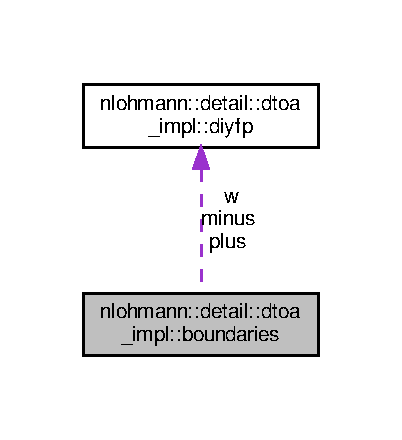
\includegraphics[width=193pt]{structnlohmann_1_1detail_1_1dtoa__impl_1_1boundaries__coll__graph}
\end{center}
\end{figure}
\subsection*{Public Attributes}
\begin{DoxyCompactItemize}
\item 
\mbox{\Hypertarget{structnlohmann_1_1detail_1_1dtoa__impl_1_1boundaries_ad1668c60aeade5f2557fafed8b8aee1a}\label{structnlohmann_1_1detail_1_1dtoa__impl_1_1boundaries_ad1668c60aeade5f2557fafed8b8aee1a}} 
\hyperlink{structnlohmann_1_1detail_1_1dtoa__impl_1_1diyfp}{diyfp} {\bfseries w}
\item 
\mbox{\Hypertarget{structnlohmann_1_1detail_1_1dtoa__impl_1_1boundaries_aec4e5028333c01f3229062f31ce16763}\label{structnlohmann_1_1detail_1_1dtoa__impl_1_1boundaries_aec4e5028333c01f3229062f31ce16763}} 
\hyperlink{structnlohmann_1_1detail_1_1dtoa__impl_1_1diyfp}{diyfp} {\bfseries minus}
\item 
\mbox{\Hypertarget{structnlohmann_1_1detail_1_1dtoa__impl_1_1boundaries_a3321ae2816a6ec5250a0d8e29f798232}\label{structnlohmann_1_1detail_1_1dtoa__impl_1_1boundaries_a3321ae2816a6ec5250a0d8e29f798232}} 
\hyperlink{structnlohmann_1_1detail_1_1dtoa__impl_1_1diyfp}{diyfp} {\bfseries plus}
\end{DoxyCompactItemize}


The documentation for this struct was generated from the following file\+:\begin{DoxyCompactItemize}
\item 
src/tools/json/json.\+hpp\end{DoxyCompactItemize}

\hypertarget{structnlohmann_1_1detail_1_1dtoa__impl_1_1cached__power}{}\section{nlohmann\+:\+:detail\+:\+:dtoa\+\_\+impl\+:\+:cached\+\_\+power Struct Reference}
\label{structnlohmann_1_1detail_1_1dtoa__impl_1_1cached__power}\index{nlohmann\+::detail\+::dtoa\+\_\+impl\+::cached\+\_\+power@{nlohmann\+::detail\+::dtoa\+\_\+impl\+::cached\+\_\+power}}
\subsection*{Public Attributes}
\begin{DoxyCompactItemize}
\item 
\mbox{\Hypertarget{structnlohmann_1_1detail_1_1dtoa__impl_1_1cached__power_a21ae81f515f5b08d5bf423775ee56074}\label{structnlohmann_1_1detail_1_1dtoa__impl_1_1cached__power_a21ae81f515f5b08d5bf423775ee56074}} 
std\+::uint64\+\_\+t {\bfseries f}
\item 
\mbox{\Hypertarget{structnlohmann_1_1detail_1_1dtoa__impl_1_1cached__power_a9e89bc89bb7bf4361f43ea27eed91d23}\label{structnlohmann_1_1detail_1_1dtoa__impl_1_1cached__power_a9e89bc89bb7bf4361f43ea27eed91d23}} 
int {\bfseries e}
\item 
\mbox{\Hypertarget{structnlohmann_1_1detail_1_1dtoa__impl_1_1cached__power_a8c1f2efed643eeaa8fae83c697a29c6a}\label{structnlohmann_1_1detail_1_1dtoa__impl_1_1cached__power_a8c1f2efed643eeaa8fae83c697a29c6a}} 
int {\bfseries k}
\end{DoxyCompactItemize}


The documentation for this struct was generated from the following file\+:\begin{DoxyCompactItemize}
\item 
src/tools/json/json.\+hpp\end{DoxyCompactItemize}

\hypertarget{classCipherTextWrapperFactory}{}\section{Cipher\+Text\+Wrapper\+Factory$<$ Ciphter\+Text\+Wrapper $>$ Class Template Reference}
\label{classCipherTextWrapperFactory}\index{Cipher\+Text\+Wrapper\+Factory$<$ Ciphter\+Text\+Wrapper $>$@{Cipher\+Text\+Wrapper\+Factory$<$ Ciphter\+Text\+Wrapper $>$}}
\subsection*{Public Member Functions}
\begin{DoxyCompactItemize}
\item 
\mbox{\Hypertarget{classCipherTextWrapperFactory_a4fa945beadaaecaa9746b081cbef555c}\label{classCipherTextWrapperFactory_a4fa945beadaaecaa9746b081cbef555c}} 
virtual void {\bfseries set\+As\+Default\+Factory} ()=0
\item 
\mbox{\Hypertarget{classCipherTextWrapperFactory_a74fad1164162787aa98a3d9a7c6351f3}\label{classCipherTextWrapperFactory_a74fad1164162787aa98a3d9a7c6351f3}} 
virtual Ciphter\+Text\+Wrapper {\bfseries empty} ()=0
\item 
\mbox{\Hypertarget{classCipherTextWrapperFactory_a742c06d87256c4af89727216f732ca03}\label{classCipherTextWrapperFactory_a742c06d87256c4af89727216f732ca03}} 
virtual Ciphter\+Text\+Wrapper {\bfseries create\+Cipher\+Text} (long x)=0
\item 
\mbox{\Hypertarget{classCipherTextWrapperFactory_afbae84b62a32db852e241c29a7b7589a}\label{classCipherTextWrapperFactory_afbae84b62a32db852e241c29a7b7589a}} 
virtual Ciphter\+Text\+Wrapper {\bfseries create\+Cipher\+Text} (const std\+::vector$<$ long $>$ \&in)=0
\item 
\mbox{\Hypertarget{classCipherTextWrapperFactory_a0781f478d2efdcd4f73b5f642f3b64a3}\label{classCipherTextWrapperFactory_a0781f478d2efdcd4f73b5f642f3b64a3}} 
virtual Ciphter\+Text\+Wrapper {\bfseries create\+Cipher\+Text} (const std\+::vector$<$ double $>$ \&in)=0
\item 
\mbox{\Hypertarget{classCipherTextWrapperFactory_a2bf5d024b47dbf24cd6da69de4490169}\label{classCipherTextWrapperFactory_a2bf5d024b47dbf24cd6da69de4490169}} 
virtual Ciphter\+Text\+Wrapper {\bfseries create\+Cipher\+Text} (const std\+::vector$<$ float $>$ \&in)=0
\item 
\mbox{\Hypertarget{classCipherTextWrapperFactory_a450db5b8bf0461a3587da2f058bd38da}\label{classCipherTextWrapperFactory_a450db5b8bf0461a3587da2f058bd38da}} 
virtual std\+::vector$<$ long $>$ {\bfseries decrypt\+Long} (const Ciphter\+Text\+Wrapper \&ctx)=0
\item 
\mbox{\Hypertarget{classCipherTextWrapperFactory_a3f82164d98d194f357f35bb556f53a88}\label{classCipherTextWrapperFactory_a3f82164d98d194f357f35bb556f53a88}} 
virtual std\+::vector$<$ double $>$ {\bfseries decrypt\+Double} (const Ciphter\+Text\+Wrapper \&ctx)=0
\item 
\mbox{\Hypertarget{classCipherTextWrapperFactory_aabc9d4f37f99a4af26f7489507bbedaa}\label{classCipherTextWrapperFactory_aabc9d4f37f99a4af26f7489507bbedaa}} 
virtual uint {\bfseries batchsize} ()=0
\item 
\mbox{\Hypertarget{classCipherTextWrapperFactory_a3789f51224da4d299c25c506848ef224}\label{classCipherTextWrapperFactory_a3789f51224da4d299c25c506848ef224}} 
virtual TensorP$<$ Ciphter\+Text\+Wrapper $>$ \hyperlink{classCipherTextWrapperFactory_a3789f51224da4d299c25c506848ef224}{create\+Cipher\+Tensor} (const std\+::vector$<$ double $>$ \&in, const \hyperlink{classShape}{Shape} \&shape, \hyperlink{classHETensorFactory}{H\+E\+Tensor\+Factory}$<$ Ciphter\+Text\+Wrapper $>$ $\ast$hetf)=0
\begin{DoxyCompactList}\small\item\em Take a 1D vector transform into the given shape and encrypt it. The 1st dimension of the same needs to line up with the batch\+Size supported by the encryption scheme. \end{DoxyCompactList}\item 
\mbox{\Hypertarget{classCipherTextWrapperFactory_adeb6353a9a9422b1fbb9c81fd10460f6}\label{classCipherTextWrapperFactory_adeb6353a9a9422b1fbb9c81fd10460f6}} 
virtual TensorP$<$ Ciphter\+Text\+Wrapper $>$ {\bfseries create\+Cipher\+Tensor} (const std\+::vector$<$ float $>$ \&in, const \hyperlink{classShape}{Shape} \&shape, \hyperlink{classHETensorFactory}{H\+E\+Tensor\+Factory}$<$ Ciphter\+Text\+Wrapper $>$ $\ast$hetf)=0
\item 
\mbox{\Hypertarget{classCipherTextWrapperFactory_ae751664fea4b4a35b8ace79c11516e14}\label{classCipherTextWrapperFactory_ae751664fea4b4a35b8ace79c11516e14}} 
virtual void {\bfseries feed\+Cipher\+Tensor} (const std\+::vector$<$ double $>$ \&in, TensorP$<$ Ciphter\+Text\+Wrapper $>$ tensor)=0
\item 
\mbox{\Hypertarget{classCipherTextWrapperFactory_af31fa14e76c55c298985dcbeb3536416}\label{classCipherTextWrapperFactory_af31fa14e76c55c298985dcbeb3536416}} 
virtual void {\bfseries feed\+Cipher\+Tensor} (const std\+::vector$<$ float $>$ \&in, TensorP$<$ Ciphter\+Text\+Wrapper $>$ tensor)=0
\item 
\mbox{\Hypertarget{classCipherTextWrapperFactory_ae6baa28f8eaee6ab89ae0d3803bdaf2e}\label{classCipherTextWrapperFactory_ae6baa28f8eaee6ab89ae0d3803bdaf2e}} 
virtual void {\bfseries feed\+Cipher\+Tensor} (const TensorP$<$ double $>$ in, TensorP$<$ Ciphter\+Text\+Wrapper $>$ tensor)=0
\item 
\mbox{\Hypertarget{classCipherTextWrapperFactory_a1aae33d3536a33fac5161b862f094123}\label{classCipherTextWrapperFactory_a1aae33d3536a33fac5161b862f094123}} 
virtual void {\bfseries feed\+Cipher\+Tensor} (const TensorP$<$ double $>$ in, \hyperlink{classTensor}{Tensor}$<$ Ciphter\+Text\+Wrapper $>$ \&tensor)=0
\item 
\mbox{\Hypertarget{classCipherTextWrapperFactory_a41a57dbe2970b399e2b9c55befec9a39}\label{classCipherTextWrapperFactory_a41a57dbe2970b399e2b9c55befec9a39}} 
void {\bfseries enable\+Refresh\+On\+High\+Noise} ()
\item 
\mbox{\Hypertarget{classCipherTextWrapperFactory_af2fd9b0b79bafca9c4a46895afcc5ccb}\label{classCipherTextWrapperFactory_af2fd9b0b79bafca9c4a46895afcc5ccb}} 
void {\bfseries disable\+Refresh\+On\+High\+Noise} ()
\item 
\mbox{\Hypertarget{classCipherTextWrapperFactory_ac4bbd9e27c7d4a49212c9002213668a7}\label{classCipherTextWrapperFactory_ac4bbd9e27c7d4a49212c9002213668a7}} 
bool {\bfseries refresh\+On\+High\+Noise\+Enabled} ()
\end{DoxyCompactItemize}


The documentation for this class was generated from the following file\+:\begin{DoxyCompactItemize}
\item 
src/architecture/\+H\+E\+Backend/Cipher\+Text\+Wrapper.\+h\end{DoxyCompactItemize}

\hypertarget{classConfig}{}\section{Config Class Reference}
\label{classConfig}\index{Config@{Config}}


Global config. Values can be retrieved with the get function. The config file will be loaded automically when the get function is called the first time. If you want it to be efficient cache the values instead of reading getting them from the config over and over.  




{\ttfamily \#include $<$Config.\+h$>$}

\subsection*{Public Member Functions}
\begin{DoxyCompactItemize}
\item 
\mbox{\Hypertarget{classConfig_a7f80dce3d79f5987b9e1e0073ab19795}\label{classConfig_a7f80dce3d79f5987b9e1e0073ab19795}} 
{\footnotesize template$<$class T $>$ }\\T {\bfseries get} (const std\+::string \&section, const std\+::string \&key)
\item 
\mbox{\Hypertarget{classConfig_aaef650a441e006c24120aae8e78b6c64}\label{classConfig_aaef650a441e006c24120aae8e78b6c64}} 
void {\bfseries operator=} (\hyperlink{classConfig}{Config} const \&)=delete
\item 
\mbox{\Hypertarget{classConfig_ad2e93ef08a872f46ca139ad28d64e2f9}\label{classConfig_ad2e93ef08a872f46ca139ad28d64e2f9}} 
{\bfseries Config} (\hyperlink{classConfig}{Config} const \&)=delete
\item 
\mbox{\Hypertarget{classConfig_a213d65cd156ab1be0697b96414cd625d}\label{classConfig_a213d65cd156ab1be0697b96414cd625d}} 
{\footnotesize template$<$$>$ }\\bool {\bfseries get} (const std\+::string \&section, const std\+::string \&key)
\item 
\mbox{\Hypertarget{classConfig_a53270a0ef7ad1e113c5af3e78579f6d6}\label{classConfig_a53270a0ef7ad1e113c5af3e78579f6d6}} 
{\footnotesize template$<$$>$ }\\long {\bfseries get} (const std\+::string \&section, const std\+::string \&key)
\item 
\mbox{\Hypertarget{classConfig_a0ae95b2baf456ffb7f7292bc094a3e2a}\label{classConfig_a0ae95b2baf456ffb7f7292bc094a3e2a}} 
{\footnotesize template$<$$>$ }\\double {\bfseries get} (const std\+::string \&section, const std\+::string \&key)
\end{DoxyCompactItemize}
\subsection*{Static Public Member Functions}
\begin{DoxyCompactItemize}
\item 
static \hyperlink{classConfig}{Config} $\ast$ \hyperlink{classConfig_a8b276bc712a71bc2febd789071974c44}{get\+Config} ()
\end{DoxyCompactItemize}


\subsection{Detailed Description}
Global config. Values can be retrieved with the get function. The config file will be loaded automically when the get function is called the first time. If you want it to be efficient cache the values instead of reading getting them from the config over and over. 

Supported datatypes and default values if the key can not be found in the config

string = \char`\"{}\char`\"{} long = 0 double = 0.\+0 bool = false 

\subsection{Member Function Documentation}
\mbox{\Hypertarget{classConfig_a8b276bc712a71bc2febd789071974c44}\label{classConfig_a8b276bc712a71bc2febd789071974c44}} 
\index{Config@{Config}!get\+Config@{get\+Config}}
\index{get\+Config@{get\+Config}!Config@{Config}}
\subsubsection{\texorpdfstring{get\+Config()}{getConfig()}}
{\footnotesize\ttfamily \hyperlink{classConfig}{Config} $\ast$ Config\+::get\+Config (\begin{DoxyParamCaption}{ }\end{DoxyParamCaption})\hspace{0.3cm}{\ttfamily [static]}}

Defaults to config.\+ini 

The documentation for this class was generated from the following files\+:\begin{DoxyCompactItemize}
\item 
src/tools/Config.\+h\item 
src/tools/Config.\+cpp\end{DoxyCompactItemize}

\hypertarget{classConvolution2D}{}\section{Convolution2D$<$ Value\+Type, Weight\+Type, Data\+Tensor\+Type, Weight\+Tensor\+Type, Converted\+Weights $>$ Class Template Reference}
\label{classConvolution2D}\index{Convolution2\+D$<$ Value\+Type, Weight\+Type, Data\+Tensor\+Type, Weight\+Tensor\+Type, Converted\+Weights $>$@{Convolution2\+D$<$ Value\+Type, Weight\+Type, Data\+Tensor\+Type, Weight\+Tensor\+Type, Converted\+Weights $>$}}


Inheritance diagram for Convolution2D$<$ Value\+Type, Weight\+Type, Data\+Tensor\+Type, Weight\+Tensor\+Type, Converted\+Weights $>$\+:
\nopagebreak
\begin{figure}[H]
\begin{center}
\leavevmode
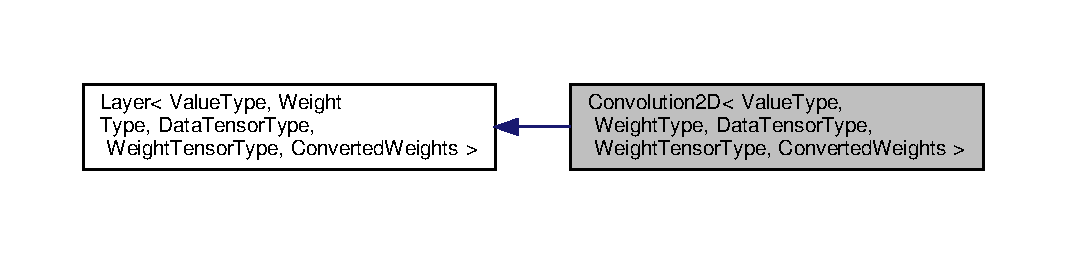
\includegraphics[width=350pt]{classConvolution2D__inherit__graph}
\end{center}
\end{figure}


Collaboration diagram for Convolution2D$<$ Value\+Type, Weight\+Type, Data\+Tensor\+Type, Weight\+Tensor\+Type, Converted\+Weights $>$\+:
\nopagebreak
\begin{figure}[H]
\begin{center}
\leavevmode
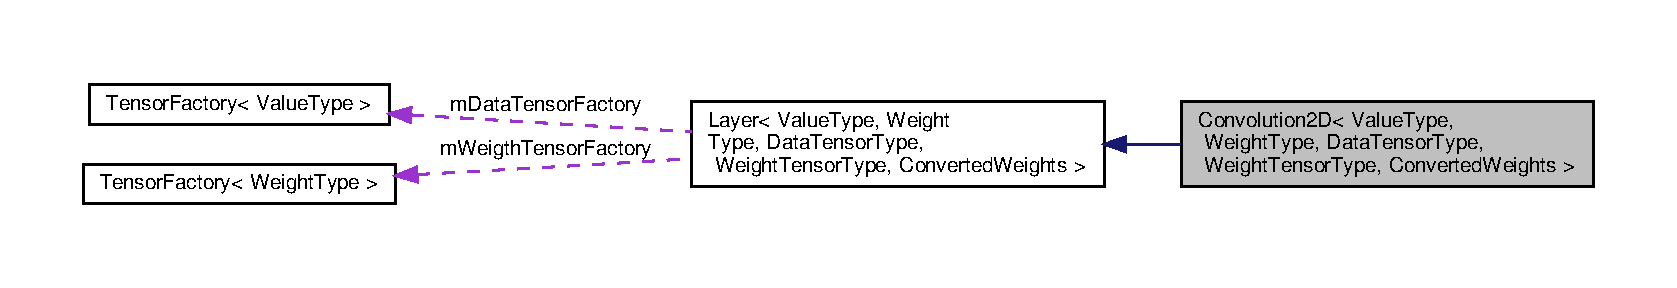
\includegraphics[width=350pt]{classConvolution2D__coll__graph}
\end{center}
\end{figure}
\subsection*{Public Member Functions}
\begin{DoxyCompactItemize}
\item 
\mbox{\Hypertarget{classConvolution2D_ad8c19607c1be356df2aca05117e33b96}\label{classConvolution2D_ad8c19607c1be356df2aca05117e33b96}} 
{\bfseries Convolution2D} (std\+::string name, ActivationP$<$ Value\+Type $>$ act, uint no\+Filters, uint filter\+Size, uint stride, P\+A\+D\+D\+I\+N\+G\+\_\+\+M\+O\+DE pad, TensorP$<$ Value\+Type $>$ input, \hyperlink{classTensorFactory}{Tensor\+Factory}$<$ Value\+Type $>$ $\ast$data\+Tensor\+Factory, \hyperlink{classTensorFactory}{Tensor\+Factory}$<$ Weight\+Type $>$ $\ast$weigth\+Tensor\+Factory)
\item 
\mbox{\Hypertarget{classConvolution2D_a54909b2da5a3fa4436d42a4d40135649}\label{classConvolution2D_a54909b2da5a3fa4436d42a4d40135649}} 
{\bfseries Convolution2D} (std\+::string name, ActivationP$<$ Value\+Type $>$ act, uint no\+Filters, uint filter\+Size, uint stride, P\+A\+D\+D\+I\+N\+G\+\_\+\+M\+O\+DE pad, \hyperlink{classTensorFactory}{Tensor\+Factory}$<$ Value\+Type $>$ $\ast$data\+Tensor\+Factory, \hyperlink{classTensorFactory}{Tensor\+Factory}$<$ Weight\+Type $>$ $\ast$weigth\+Tensor\+Factory)
\item 
\mbox{\Hypertarget{classConvolution2D_af9bd71d1356e708f9872d48279f6713a}\label{classConvolution2D_af9bd71d1356e708f9872d48279f6713a}} 
{\bfseries Convolution2D} (std\+::string name, ActivationP$<$ Value\+Type $>$ act, uint no\+Filters, uint filter\+Size, uint stride, P\+A\+D\+D\+I\+N\+G\+\_\+\+M\+O\+DE pad, TensorP$<$ Value\+Type $>$ input)
\item 
\mbox{\Hypertarget{classConvolution2D_a3ac1b953a9fb5eb2f48faf0229933531}\label{classConvolution2D_a3ac1b953a9fb5eb2f48faf0229933531}} 
{\bfseries Convolution2D} (std\+::string name, ActivationP$<$ Value\+Type $>$ act, uint no\+Filters, uint filter\+Size, uint stride, P\+A\+D\+D\+I\+N\+G\+\_\+\+M\+O\+DE pad)
\item 
\mbox{\Hypertarget{classConvolution2D_af69229ab131e71abc743057699edfb42}\label{classConvolution2D_af69229ab131e71abc743057699edfb42}} 
{\bfseries Convolution2D} (std\+::string name, ActivationP$<$ Value\+Type $>$ act, uint no\+Filters, uint filter\+Size, uint stride, P\+A\+D\+D\+I\+N\+G\+\_\+\+M\+O\+DE pad, TensorP$<$ Value\+Type $>$ input, Tensor\+FactoryP$<$ Value\+Type $>$ data\+Tensor\+Factory, Tensor\+FactoryP$<$ Weight\+Type $>$ weight\+Tensor\+Factory)
\item 
\mbox{\Hypertarget{classConvolution2D_aa4d634085ca7ab3d1945185d8c908dc9}\label{classConvolution2D_aa4d634085ca7ab3d1945185d8c908dc9}} 
{\bfseries Convolution2D} (std\+::string name, ActivationP$<$ Value\+Type $>$ act, uint no\+Filters, uint filter\+Size, uint stride, P\+A\+D\+D\+I\+N\+G\+\_\+\+M\+O\+DE pad, Tensor\+FactoryP$<$ Value\+Type $>$ data\+Tensor\+Factory, Tensor\+FactoryP$<$ Weight\+Type $>$ weight\+Tensor\+Factory)
\item 
\mbox{\Hypertarget{classConvolution2D_a713b56c33b0595d1095397129391e70e}\label{classConvolution2D_a713b56c33b0595d1095397129391e70e}} 
\hyperlink{classShape}{Shape} {\bfseries output\+Shape} () override
\item 
\mbox{\Hypertarget{classConvolution2D_a2031c3d59486ce80626f04ae21a34162}\label{classConvolution2D_a2031c3d59486ce80626f04ae21a34162}} 
void {\bfseries feed\+Forward} () override
\item 
\mbox{\Hypertarget{classConvolution2D_aa3084202934370bcb7a81894657dc51c}\label{classConvolution2D_aa3084202934370bcb7a81894657dc51c}} 
void {\bfseries load\+Weights} (std\+::string path, std\+::string file\+Name) override
\item 
\mbox{\Hypertarget{classConvolution2D_a1d8cfc56655d5b2321a27a8e99a8d2cf}\label{classConvolution2D_a1d8cfc56655d5b2321a27a8e99a8d2cf}} 
void {\bfseries load\+Weights} (std\+::string path) override
\item 
\mbox{\Hypertarget{classConvolution2D_a60f6c470cee849147107690c4662ba0f}\label{classConvolution2D_a60f6c470cee849147107690c4662ba0f}} 
virtual void {\bfseries random\+Init} () override
\item 
\mbox{\Hypertarget{classConvolution2D_ae0fdd1ea63c8c9de35069d2ae115b114}\label{classConvolution2D_ae0fdd1ea63c8c9de35069d2ae115b114}} 
void {\bfseries description} () override
\item 
\mbox{\Hypertarget{classConvolution2D_a32c8da64840fa7a3527e0b4180faaff8}\label{classConvolution2D_a32c8da64840fa7a3527e0b4180faaff8}} 
virtual std\+::vector$<$ TensorP$<$ Weight\+Type $>$ $>$ \hyperlink{classConvolution2D_a32c8da64840fa7a3527e0b4180faaff8}{all\+Weights} () override
\begin{DoxyCompactList}\small\item\em Returns weights, biases. \end{DoxyCompactList}\end{DoxyCompactItemize}
\subsection*{Additional Inherited Members}


The documentation for this class was generated from the following file\+:\begin{DoxyCompactItemize}
\item 
src/architecture/Layer\+Impl.\+h\end{DoxyCompactItemize}

\hypertarget{classData}{}\section{Data$<$ Data\+Type, Label\+Type $>$ Class Template Reference}
\label{classData}\index{Data$<$ Data\+Type, Label\+Type $>$@{Data$<$ Data\+Type, Label\+Type $>$}}
\subsection*{Public Member Functions}
\begin{DoxyCompactItemize}
\item 
\mbox{\Hypertarget{classData_a31b11247eb4d6bf3cff069ea5d5fa04b}\label{classData_a31b11247eb4d6bf3cff069ea5d5fa04b}} 
{\bfseries Data} (std\+::string set)
\item 
\mbox{\Hypertarget{classData_a134973a2f111a6104ba26206a73c1f6c}\label{classData_a134973a2f111a6104ba26206a73c1f6c}} 
TensorP$<$ Data\+Type $>$ {\bfseries grab\+Data} (std\+::string type)
\item 
\mbox{\Hypertarget{classData_abefa2813d1f699581768f0675767286d}\label{classData_abefa2813d1f699581768f0675767286d}} 
TensorP$<$ Label\+Type $>$ {\bfseries grab\+Labels} (std\+::string type)
\end{DoxyCompactItemize}


The documentation for this class was generated from the following file\+:\begin{DoxyCompactItemize}
\item 
src/data/Datasets.\+h\end{DoxyCompactItemize}

\hypertarget{classDense}{}\section{Dense$<$ Value\+Type, Weight\+Type, Data\+Tensor\+Type, Weight\+Tensor\+Type, Converted\+Weights $>$ Class Template Reference}
\label{classDense}\index{Dense$<$ Value\+Type, Weight\+Type, Data\+Tensor\+Type, Weight\+Tensor\+Type, Converted\+Weights $>$@{Dense$<$ Value\+Type, Weight\+Type, Data\+Tensor\+Type, Weight\+Tensor\+Type, Converted\+Weights $>$}}


Inheritance diagram for Dense$<$ Value\+Type, Weight\+Type, Data\+Tensor\+Type, Weight\+Tensor\+Type, Converted\+Weights $>$\+:
\nopagebreak
\begin{figure}[H]
\begin{center}
\leavevmode
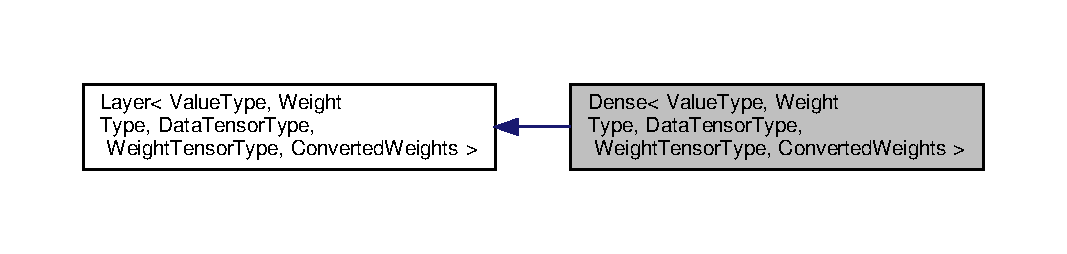
\includegraphics[width=350pt]{classDense__inherit__graph}
\end{center}
\end{figure}


Collaboration diagram for Dense$<$ Value\+Type, Weight\+Type, Data\+Tensor\+Type, Weight\+Tensor\+Type, Converted\+Weights $>$\+:
\nopagebreak
\begin{figure}[H]
\begin{center}
\leavevmode
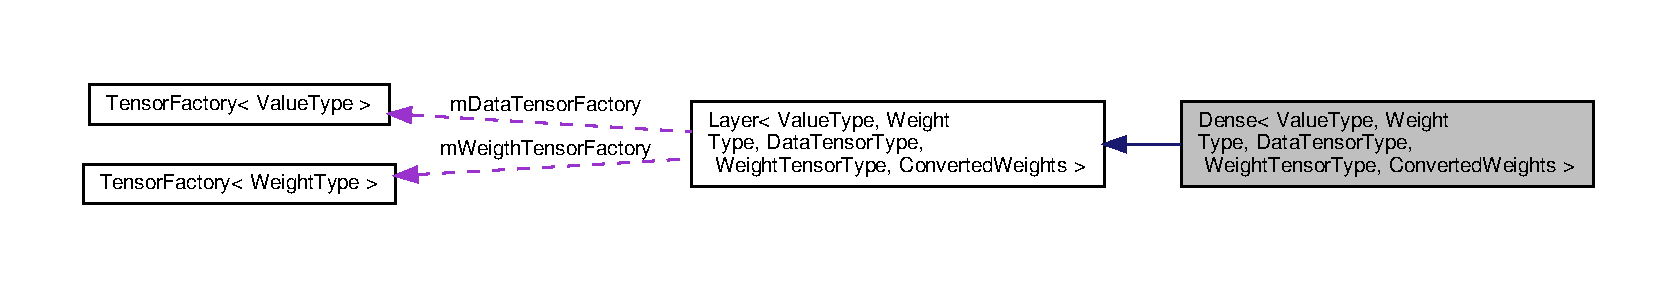
\includegraphics[width=350pt]{classDense__coll__graph}
\end{center}
\end{figure}
\subsection*{Public Member Functions}
\begin{DoxyCompactItemize}
\item 
\mbox{\Hypertarget{classDense_accea6109fab79bbd26800c7367e26857}\label{classDense_accea6109fab79bbd26800c7367e26857}} 
{\bfseries Dense} (std\+::string name, ActivationP$<$ Value\+Type $>$ act, uint no\+Neurons, TensorP$<$ Value\+Type $>$ input, \hyperlink{classTensorFactory}{Tensor\+Factory}$<$ Value\+Type $>$ $\ast$data\+Tensor\+Factory, \hyperlink{classTensorFactory}{Tensor\+Factory}$<$ Weight\+Type $>$ $\ast$weigth\+Tensor\+Factory)
\item 
\mbox{\Hypertarget{classDense_acfbc00b146e67de2f82502ee0696eeab}\label{classDense_acfbc00b146e67de2f82502ee0696eeab}} 
{\bfseries Dense} (std\+::string name, ActivationP$<$ Value\+Type $>$ act, uint no\+Neurons, \hyperlink{classTensorFactory}{Tensor\+Factory}$<$ Value\+Type $>$ $\ast$data\+Tensor\+Factory, \hyperlink{classTensorFactory}{Tensor\+Factory}$<$ Weight\+Type $>$ $\ast$weigth\+Tensor\+Factory)
\item 
\mbox{\Hypertarget{classDense_a3ee6122ece50f43ce752d244b5207aaf}\label{classDense_a3ee6122ece50f43ce752d244b5207aaf}} 
{\bfseries Dense} (std\+::string name, ActivationP$<$ Value\+Type $>$ act, uint no\+Neurons, TensorP$<$ Value\+Type $>$ input)
\item 
\mbox{\Hypertarget{classDense_a81f4283f40d537465f7d6da62b6749b6}\label{classDense_a81f4283f40d537465f7d6da62b6749b6}} 
{\bfseries Dense} (std\+::string name, ActivationP$<$ Value\+Type $>$ act, uint no\+Neurons)
\item 
\mbox{\Hypertarget{classDense_af1260b026220a907e2d97933acb3c016}\label{classDense_af1260b026220a907e2d97933acb3c016}} 
{\bfseries Dense} (std\+::string name, ActivationP$<$ Value\+Type $>$ act, uint no\+Neurons, TensorP$<$ Value\+Type $>$ input, Tensor\+FactoryP$<$ Value\+Type $>$ data\+Tensor\+Factory, Tensor\+FactoryP$<$ Weight\+Type $>$ weight\+Tensor\+Factory)
\item 
\mbox{\Hypertarget{classDense_a7a6c03d898aa2fd991ce488bfe2badc4}\label{classDense_a7a6c03d898aa2fd991ce488bfe2badc4}} 
{\bfseries Dense} (std\+::string name, ActivationP$<$ Value\+Type $>$ act, uint no\+Neurons, Tensor\+FactoryP$<$ Value\+Type $>$ data\+Tensor\+Factory, Tensor\+FactoryP$<$ Weight\+Type $>$ weight\+Tensor\+Factory)
\item 
\mbox{\Hypertarget{classDense_a085651662d9c97063d5ef89956b03496}\label{classDense_a085651662d9c97063d5ef89956b03496}} 
\hyperlink{classShape}{Shape} {\bfseries output\+Shape} () override
\item 
\mbox{\Hypertarget{classDense_a4e443f667dc72bb595f85e7af3f3a7aa}\label{classDense_a4e443f667dc72bb595f85e7af3f3a7aa}} 
void {\bfseries feed\+Forward} () override
\item 
\mbox{\Hypertarget{classDense_a6254c14c1bce21c5c1905388642160cf}\label{classDense_a6254c14c1bce21c5c1905388642160cf}} 
void {\bfseries load\+Weights} (std\+::string path, std\+::string file\+Name)
\item 
\mbox{\Hypertarget{classDense_a503236232088bef7f7f4ed2902c8e32d}\label{classDense_a503236232088bef7f7f4ed2902c8e32d}} 
void {\bfseries load\+Weights} (std\+::string path)
\item 
\mbox{\Hypertarget{classDense_a6a71e42b57250b30277d3a372eeae366}\label{classDense_a6a71e42b57250b30277d3a372eeae366}} 
virtual void {\bfseries random\+Init} () override
\item 
\mbox{\Hypertarget{classDense_aa21053ebb51564c7761b433bcb0e9006}\label{classDense_aa21053ebb51564c7761b433bcb0e9006}} 
void {\bfseries description} ()
\item 
\mbox{\Hypertarget{classDense_a03631983df825324bdf4b5e57a23bbbf}\label{classDense_a03631983df825324bdf4b5e57a23bbbf}} 
virtual std\+::vector$<$ TensorP$<$ Weight\+Type $>$ $>$ \hyperlink{classDense_a03631983df825324bdf4b5e57a23bbbf}{all\+Weights} () override
\begin{DoxyCompactList}\small\item\em Returns weights, biases. \end{DoxyCompactList}\end{DoxyCompactItemize}
\subsection*{Additional Inherited Members}


The documentation for this class was generated from the following file\+:\begin{DoxyCompactItemize}
\item 
src/architecture/Layer\+Impl.\+h\end{DoxyCompactItemize}

\hypertarget{structnlohmann_1_1detail_1_1detector}{}\section{nlohmann\+:\+:detail\+:\+:detector$<$ Default, Always\+Void, Op, Args $>$ Struct Template Reference}
\label{structnlohmann_1_1detail_1_1detector}\index{nlohmann\+::detail\+::detector$<$ Default, Always\+Void, Op, Args $>$@{nlohmann\+::detail\+::detector$<$ Default, Always\+Void, Op, Args $>$}}
\subsection*{Public Types}
\begin{DoxyCompactItemize}
\item 
\mbox{\Hypertarget{structnlohmann_1_1detail_1_1detector_a5a132aab543d1706e2439268faf8d487}\label{structnlohmann_1_1detail_1_1detector_a5a132aab543d1706e2439268faf8d487}} 
using {\bfseries value\+\_\+t} = std\+::false\+\_\+type
\item 
\mbox{\Hypertarget{structnlohmann_1_1detail_1_1detector_a0cd69423587748bf3d3d702cc7b7c2ce}\label{structnlohmann_1_1detail_1_1detector_a0cd69423587748bf3d3d702cc7b7c2ce}} 
using {\bfseries type} = Default
\end{DoxyCompactItemize}


The documentation for this struct was generated from the following file\+:\begin{DoxyCompactItemize}
\item 
src/tools/json/json.\+hpp\end{DoxyCompactItemize}

\hypertarget{structnlohmann_1_1detail_1_1detector_3_01Default_00_01void__t_3_01Op_3_01Args_8_8_8_01_4_01_4_00_01Op_00_01Args_8_8_8_01_4}{}\section{nlohmann\+:\+:detail\+:\+:detector$<$ Default, void\+\_\+t$<$ Op$<$ Args... $>$ $>$, Op, Args... $>$ Struct Template Reference}
\label{structnlohmann_1_1detail_1_1detector_3_01Default_00_01void__t_3_01Op_3_01Args_8_8_8_01_4_01_4_00_01Op_00_01Args_8_8_8_01_4}\index{nlohmann\+::detail\+::detector$<$ Default, void\+\_\+t$<$ Op$<$ Args... $>$ $>$, Op, Args... $>$@{nlohmann\+::detail\+::detector$<$ Default, void\+\_\+t$<$ Op$<$ Args... $>$ $>$, Op, Args... $>$}}
\subsection*{Public Types}
\begin{DoxyCompactItemize}
\item 
\mbox{\Hypertarget{structnlohmann_1_1detail_1_1detector_3_01Default_00_01void__t_3_01Op_3_01Args_8_8_8_01_4_01_4_00_01Op_00_01Args_8_8_8_01_4_ab748f9f00bb31bee4978a033589f8c85}\label{structnlohmann_1_1detail_1_1detector_3_01Default_00_01void__t_3_01Op_3_01Args_8_8_8_01_4_01_4_00_01Op_00_01Args_8_8_8_01_4_ab748f9f00bb31bee4978a033589f8c85}} 
using {\bfseries value\+\_\+t} = std\+::true\+\_\+type
\item 
\mbox{\Hypertarget{structnlohmann_1_1detail_1_1detector_3_01Default_00_01void__t_3_01Op_3_01Args_8_8_8_01_4_01_4_00_01Op_00_01Args_8_8_8_01_4_a5afd6a40e94dde21d120ac646468c495}\label{structnlohmann_1_1detail_1_1detector_3_01Default_00_01void__t_3_01Op_3_01Args_8_8_8_01_4_01_4_00_01Op_00_01Args_8_8_8_01_4_a5afd6a40e94dde21d120ac646468c495}} 
using {\bfseries type} = Op$<$ Args... $>$
\end{DoxyCompactItemize}


The documentation for this struct was generated from the following file\+:\begin{DoxyCompactItemize}
\item 
src/tools/json/json.\+hpp\end{DoxyCompactItemize}

\hypertarget{structnlohmann_1_1detail_1_1dtoa__impl_1_1diyfp}{}\section{nlohmann\+:\+:detail\+:\+:dtoa\+\_\+impl\+:\+:diyfp Struct Reference}
\label{structnlohmann_1_1detail_1_1dtoa__impl_1_1diyfp}\index{nlohmann\+::detail\+::dtoa\+\_\+impl\+::diyfp@{nlohmann\+::detail\+::dtoa\+\_\+impl\+::diyfp}}
\subsection*{Public Member Functions}
\begin{DoxyCompactItemize}
\item 
\mbox{\Hypertarget{structnlohmann_1_1detail_1_1dtoa__impl_1_1diyfp_ad8798a8823a49c8412f0fada9892c918}\label{structnlohmann_1_1detail_1_1dtoa__impl_1_1diyfp_ad8798a8823a49c8412f0fada9892c918}} 
constexpr {\bfseries diyfp} (std\+::uint64\+\_\+t f\+\_\+, int e\+\_\+) noexcept
\end{DoxyCompactItemize}
\subsection*{Static Public Member Functions}
\begin{DoxyCompactItemize}
\item 
static \hyperlink{structnlohmann_1_1detail_1_1dtoa__impl_1_1diyfp}{diyfp} \hyperlink{structnlohmann_1_1detail_1_1dtoa__impl_1_1diyfp_aeb26771af54ad73598c1a0430d65d884}{sub} (const \hyperlink{structnlohmann_1_1detail_1_1dtoa__impl_1_1diyfp}{diyfp} \&x, const \hyperlink{structnlohmann_1_1detail_1_1dtoa__impl_1_1diyfp}{diyfp} \&y) noexcept
\begin{DoxyCompactList}\small\item\em returns x -\/ y \end{DoxyCompactList}\item 
static \hyperlink{structnlohmann_1_1detail_1_1dtoa__impl_1_1diyfp}{diyfp} \hyperlink{structnlohmann_1_1detail_1_1dtoa__impl_1_1diyfp_aa5f250d12ce89c81fdb08900c6a823e8}{mul} (const \hyperlink{structnlohmann_1_1detail_1_1dtoa__impl_1_1diyfp}{diyfp} \&x, const \hyperlink{structnlohmann_1_1detail_1_1dtoa__impl_1_1diyfp}{diyfp} \&y) noexcept
\begin{DoxyCompactList}\small\item\em returns x $\ast$ y \end{DoxyCompactList}\item 
static \hyperlink{structnlohmann_1_1detail_1_1dtoa__impl_1_1diyfp}{diyfp} \hyperlink{structnlohmann_1_1detail_1_1dtoa__impl_1_1diyfp_a2246b5b40c7c6992153ef174063d6aa6}{normalize} (\hyperlink{structnlohmann_1_1detail_1_1dtoa__impl_1_1diyfp}{diyfp} x) noexcept
\begin{DoxyCompactList}\small\item\em normalize x such that the significand is $>$= 2$^\wedge$(q-\/1) \end{DoxyCompactList}\item 
static \hyperlink{structnlohmann_1_1detail_1_1dtoa__impl_1_1diyfp}{diyfp} \hyperlink{structnlohmann_1_1detail_1_1dtoa__impl_1_1diyfp_a6b6665e467ebabe0c0f7418d3fe4b118}{normalize\+\_\+to} (const \hyperlink{structnlohmann_1_1detail_1_1dtoa__impl_1_1diyfp}{diyfp} \&x, const int target\+\_\+exponent) noexcept
\begin{DoxyCompactList}\small\item\em normalize x such that the result has the exponent E \end{DoxyCompactList}\end{DoxyCompactItemize}
\subsection*{Public Attributes}
\begin{DoxyCompactItemize}
\item 
\mbox{\Hypertarget{structnlohmann_1_1detail_1_1dtoa__impl_1_1diyfp_aea90459e340a231ca31d46946803ef51}\label{structnlohmann_1_1detail_1_1dtoa__impl_1_1diyfp_aea90459e340a231ca31d46946803ef51}} 
std\+::uint64\+\_\+t {\bfseries f} = 0
\item 
\mbox{\Hypertarget{structnlohmann_1_1detail_1_1dtoa__impl_1_1diyfp_ae22e170815983961447c429f324c944d}\label{structnlohmann_1_1detail_1_1dtoa__impl_1_1diyfp_ae22e170815983961447c429f324c944d}} 
int {\bfseries e} = 0
\end{DoxyCompactItemize}
\subsection*{Static Public Attributes}
\begin{DoxyCompactItemize}
\item 
\mbox{\Hypertarget{structnlohmann_1_1detail_1_1dtoa__impl_1_1diyfp_a03682754b06ed4f30b263119eecc2d52}\label{structnlohmann_1_1detail_1_1dtoa__impl_1_1diyfp_a03682754b06ed4f30b263119eecc2d52}} 
static constexpr int {\bfseries k\+Precision} = 64
\end{DoxyCompactItemize}


\subsection{Member Function Documentation}
\mbox{\Hypertarget{structnlohmann_1_1detail_1_1dtoa__impl_1_1diyfp_aa5f250d12ce89c81fdb08900c6a823e8}\label{structnlohmann_1_1detail_1_1dtoa__impl_1_1diyfp_aa5f250d12ce89c81fdb08900c6a823e8}} 
\index{nlohmann\+::detail\+::dtoa\+\_\+impl\+::diyfp@{nlohmann\+::detail\+::dtoa\+\_\+impl\+::diyfp}!mul@{mul}}
\index{mul@{mul}!nlohmann\+::detail\+::dtoa\+\_\+impl\+::diyfp@{nlohmann\+::detail\+::dtoa\+\_\+impl\+::diyfp}}
\subsubsection{\texorpdfstring{mul()}{mul()}}
{\footnotesize\ttfamily static \hyperlink{structnlohmann_1_1detail_1_1dtoa__impl_1_1diyfp}{diyfp} nlohmann\+::detail\+::dtoa\+\_\+impl\+::diyfp\+::mul (\begin{DoxyParamCaption}\item[{const \hyperlink{structnlohmann_1_1detail_1_1dtoa__impl_1_1diyfp}{diyfp} \&}]{x,  }\item[{const \hyperlink{structnlohmann_1_1detail_1_1dtoa__impl_1_1diyfp}{diyfp} \&}]{y }\end{DoxyParamCaption})\hspace{0.3cm}{\ttfamily [inline]}, {\ttfamily [static]}, {\ttfamily [noexcept]}}



returns x $\ast$ y 

\begin{DoxyNote}{Note}
The result is rounded. (Only the upper q bits are returned.) 
\end{DoxyNote}
\mbox{\Hypertarget{structnlohmann_1_1detail_1_1dtoa__impl_1_1diyfp_a2246b5b40c7c6992153ef174063d6aa6}\label{structnlohmann_1_1detail_1_1dtoa__impl_1_1diyfp_a2246b5b40c7c6992153ef174063d6aa6}} 
\index{nlohmann\+::detail\+::dtoa\+\_\+impl\+::diyfp@{nlohmann\+::detail\+::dtoa\+\_\+impl\+::diyfp}!normalize@{normalize}}
\index{normalize@{normalize}!nlohmann\+::detail\+::dtoa\+\_\+impl\+::diyfp@{nlohmann\+::detail\+::dtoa\+\_\+impl\+::diyfp}}
\subsubsection{\texorpdfstring{normalize()}{normalize()}}
{\footnotesize\ttfamily static \hyperlink{structnlohmann_1_1detail_1_1dtoa__impl_1_1diyfp}{diyfp} nlohmann\+::detail\+::dtoa\+\_\+impl\+::diyfp\+::normalize (\begin{DoxyParamCaption}\item[{\hyperlink{structnlohmann_1_1detail_1_1dtoa__impl_1_1diyfp}{diyfp}}]{x }\end{DoxyParamCaption})\hspace{0.3cm}{\ttfamily [inline]}, {\ttfamily [static]}, {\ttfamily [noexcept]}}



normalize x such that the significand is $>$= 2$^\wedge$(q-\/1) 

\begin{DoxyPrecond}{Precondition}
x.\+f != 0 
\end{DoxyPrecond}
\mbox{\Hypertarget{structnlohmann_1_1detail_1_1dtoa__impl_1_1diyfp_a6b6665e467ebabe0c0f7418d3fe4b118}\label{structnlohmann_1_1detail_1_1dtoa__impl_1_1diyfp_a6b6665e467ebabe0c0f7418d3fe4b118}} 
\index{nlohmann\+::detail\+::dtoa\+\_\+impl\+::diyfp@{nlohmann\+::detail\+::dtoa\+\_\+impl\+::diyfp}!normalize\+\_\+to@{normalize\+\_\+to}}
\index{normalize\+\_\+to@{normalize\+\_\+to}!nlohmann\+::detail\+::dtoa\+\_\+impl\+::diyfp@{nlohmann\+::detail\+::dtoa\+\_\+impl\+::diyfp}}
\subsubsection{\texorpdfstring{normalize\+\_\+to()}{normalize\_to()}}
{\footnotesize\ttfamily static \hyperlink{structnlohmann_1_1detail_1_1dtoa__impl_1_1diyfp}{diyfp} nlohmann\+::detail\+::dtoa\+\_\+impl\+::diyfp\+::normalize\+\_\+to (\begin{DoxyParamCaption}\item[{const \hyperlink{structnlohmann_1_1detail_1_1dtoa__impl_1_1diyfp}{diyfp} \&}]{x,  }\item[{const int}]{target\+\_\+exponent }\end{DoxyParamCaption})\hspace{0.3cm}{\ttfamily [inline]}, {\ttfamily [static]}, {\ttfamily [noexcept]}}



normalize x such that the result has the exponent E 

\begin{DoxyPrecond}{Precondition}
e $>$= x.\+e and the upper e -\/ x.\+e bits of x.\+f must be zero. 
\end{DoxyPrecond}
\mbox{\Hypertarget{structnlohmann_1_1detail_1_1dtoa__impl_1_1diyfp_aeb26771af54ad73598c1a0430d65d884}\label{structnlohmann_1_1detail_1_1dtoa__impl_1_1diyfp_aeb26771af54ad73598c1a0430d65d884}} 
\index{nlohmann\+::detail\+::dtoa\+\_\+impl\+::diyfp@{nlohmann\+::detail\+::dtoa\+\_\+impl\+::diyfp}!sub@{sub}}
\index{sub@{sub}!nlohmann\+::detail\+::dtoa\+\_\+impl\+::diyfp@{nlohmann\+::detail\+::dtoa\+\_\+impl\+::diyfp}}
\subsubsection{\texorpdfstring{sub()}{sub()}}
{\footnotesize\ttfamily static \hyperlink{structnlohmann_1_1detail_1_1dtoa__impl_1_1diyfp}{diyfp} nlohmann\+::detail\+::dtoa\+\_\+impl\+::diyfp\+::sub (\begin{DoxyParamCaption}\item[{const \hyperlink{structnlohmann_1_1detail_1_1dtoa__impl_1_1diyfp}{diyfp} \&}]{x,  }\item[{const \hyperlink{structnlohmann_1_1detail_1_1dtoa__impl_1_1diyfp}{diyfp} \&}]{y }\end{DoxyParamCaption})\hspace{0.3cm}{\ttfamily [inline]}, {\ttfamily [static]}, {\ttfamily [noexcept]}}



returns x -\/ y 

\begin{DoxyPrecond}{Precondition}
x.\+e == y.\+e and x.\+f $>$= y.\+f 
\end{DoxyPrecond}


The documentation for this struct was generated from the following file\+:\begin{DoxyCompactItemize}
\item 
src/tools/json/json.\+hpp\end{DoxyCompactItemize}

\hypertarget{classnlohmann_1_1detail_1_1exception}{}\section{nlohmann\+:\+:detail\+:\+:exception Class Reference}
\label{classnlohmann_1_1detail_1_1exception}\index{nlohmann\+::detail\+::exception@{nlohmann\+::detail\+::exception}}


general exception of the \hyperlink{classnlohmann_1_1basic__json}{basic\+\_\+json} class  




{\ttfamily \#include $<$json.\+hpp$>$}



Inheritance diagram for nlohmann\+:\+:detail\+:\+:exception\+:
\nopagebreak
\begin{figure}[H]
\begin{center}
\leavevmode
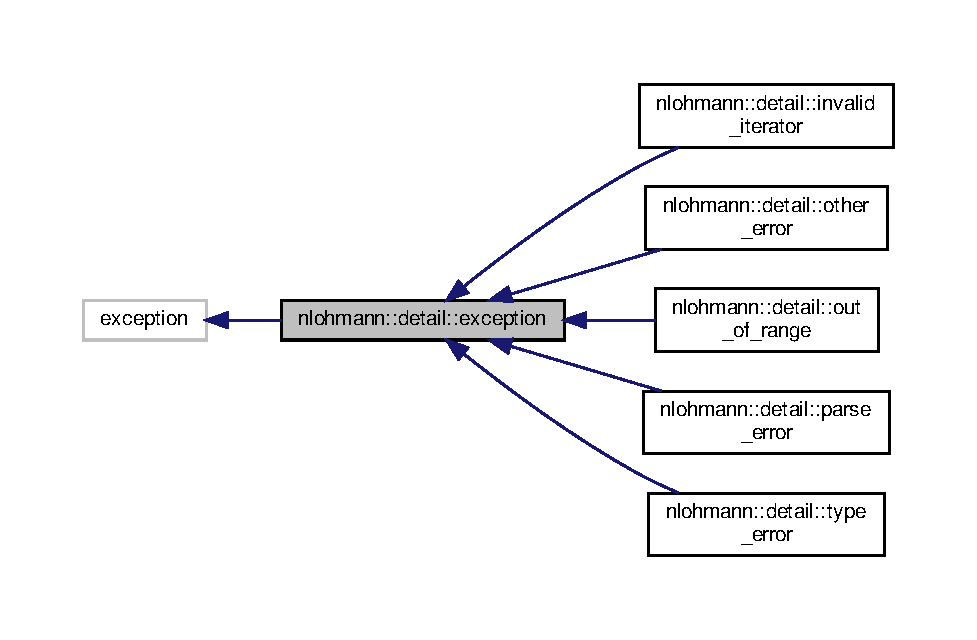
\includegraphics[width=350pt]{classnlohmann_1_1detail_1_1exception__inherit__graph}
\end{center}
\end{figure}


Collaboration diagram for nlohmann\+:\+:detail\+:\+:exception\+:
\nopagebreak
\begin{figure}[H]
\begin{center}
\leavevmode
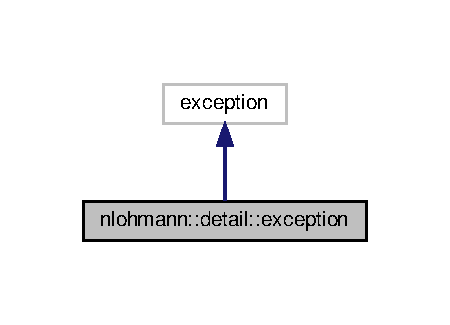
\includegraphics[width=216pt]{classnlohmann_1_1detail_1_1exception__coll__graph}
\end{center}
\end{figure}
\subsection*{Public Member Functions}
\begin{DoxyCompactItemize}
\item 
\mbox{\Hypertarget{classnlohmann_1_1detail_1_1exception_a0672c25ecdf14d1a071d4d6478a65af0}\label{classnlohmann_1_1detail_1_1exception_a0672c25ecdf14d1a071d4d6478a65af0}} 
const char $\ast$ \hyperlink{classnlohmann_1_1detail_1_1exception_a0672c25ecdf14d1a071d4d6478a65af0}{what} () const noexcept override
\begin{DoxyCompactList}\small\item\em returns the explanatory string \end{DoxyCompactList}\end{DoxyCompactItemize}
\subsection*{Public Attributes}
\begin{DoxyCompactItemize}
\item 
\mbox{\Hypertarget{classnlohmann_1_1detail_1_1exception_a0d4589a3fb54e81646d986c05efa3b9a}\label{classnlohmann_1_1detail_1_1exception_a0d4589a3fb54e81646d986c05efa3b9a}} 
const int \hyperlink{classnlohmann_1_1detail_1_1exception_a0d4589a3fb54e81646d986c05efa3b9a}{id}
\begin{DoxyCompactList}\small\item\em the id of the exception \end{DoxyCompactList}\end{DoxyCompactItemize}
\subsection*{Protected Member Functions}
\begin{DoxyCompactItemize}
\item 
\mbox{\Hypertarget{classnlohmann_1_1detail_1_1exception_ae323ad0d53bc724414c2233164e65657}\label{classnlohmann_1_1detail_1_1exception_ae323ad0d53bc724414c2233164e65657}} 
{\bfseries exception} (int id\+\_\+, const char $\ast$what\+\_\+arg)
\end{DoxyCompactItemize}
\subsection*{Static Protected Member Functions}
\begin{DoxyCompactItemize}
\item 
\mbox{\Hypertarget{classnlohmann_1_1detail_1_1exception_abf41a7e9178356314082284e6cfea278}\label{classnlohmann_1_1detail_1_1exception_abf41a7e9178356314082284e6cfea278}} 
static \hyperlink{namespacenlohmann_1_1detail_a1ed8fc6239da25abcaf681d30ace4985ab45cffe084dd3d20d928bee85e7b0f21}{std\+::string} {\bfseries name} (const \hyperlink{namespacenlohmann_1_1detail_a1ed8fc6239da25abcaf681d30ace4985ab45cffe084dd3d20d928bee85e7b0f21}{std\+::string} \&ename, int id\+\_\+)
\end{DoxyCompactItemize}


\subsection{Detailed Description}
general exception of the \hyperlink{classnlohmann_1_1basic__json}{basic\+\_\+json} class 

This class is an extension of {\ttfamily std\+::exception} objects with a member {\itshape id} for exception ids. It is used as the base class for all exceptions thrown by the \hyperlink{classnlohmann_1_1basic__json}{basic\+\_\+json} class. This class can hence be used as \char`\"{}wildcard\char`\"{} to catch exceptions.

Subclasses\+:
\begin{DoxyItemize}
\item \hyperlink{classnlohmann_1_1detail_1_1parse__error}{parse\+\_\+error} for exceptions indicating a parse error
\item \hyperlink{classnlohmann_1_1detail_1_1invalid__iterator}{invalid\+\_\+iterator} for exceptions indicating errors with iterators
\item \hyperlink{classnlohmann_1_1detail_1_1type__error}{type\+\_\+error} for exceptions indicating executing a member function with a wrong type
\item \hyperlink{classnlohmann_1_1detail_1_1out__of__range}{out\+\_\+of\+\_\+range} for exceptions indicating access out of the defined range
\item \hyperlink{classnlohmann_1_1detail_1_1other__error}{other\+\_\+error} for exceptions indicating other library errors
\end{DoxyItemize}

\{The following code shows how arbitrary library exceptions can be caught.,exception\}

\begin{DoxySince}{Since}
version 3.\+0.\+0 
\end{DoxySince}


The documentation for this class was generated from the following file\+:\begin{DoxyCompactItemize}
\item 
src/tools/json/json.\+hpp\end{DoxyCompactItemize}

\hypertarget{structnlohmann_1_1detail_1_1external__constructor}{}\section{nlohmann\+:\+:detail\+:\+:external\+\_\+constructor$<$ value\+\_\+t $>$ Struct Template Reference}
\label{structnlohmann_1_1detail_1_1external__constructor}\index{nlohmann\+::detail\+::external\+\_\+constructor$<$ value\+\_\+t $>$@{nlohmann\+::detail\+::external\+\_\+constructor$<$ value\+\_\+t $>$}}


The documentation for this struct was generated from the following file\+:\begin{DoxyCompactItemize}
\item 
src/tools/json/json.\+hpp\end{DoxyCompactItemize}

\hypertarget{structnlohmann_1_1detail_1_1external__constructor_3_01value__t_1_1array_01_4}{}\section{nlohmann\+:\+:detail\+:\+:external\+\_\+constructor$<$ value\+\_\+t\+:\+:array $>$ Struct Template Reference}
\label{structnlohmann_1_1detail_1_1external__constructor_3_01value__t_1_1array_01_4}\index{nlohmann\+::detail\+::external\+\_\+constructor$<$ value\+\_\+t\+::array $>$@{nlohmann\+::detail\+::external\+\_\+constructor$<$ value\+\_\+t\+::array $>$}}
\subsection*{Static Public Member Functions}
\begin{DoxyCompactItemize}
\item 
\mbox{\Hypertarget{structnlohmann_1_1detail_1_1external__constructor_3_01value__t_1_1array_01_4_abfb2a6eec0bc21e8a7438546aebc55d8}\label{structnlohmann_1_1detail_1_1external__constructor_3_01value__t_1_1array_01_4_abfb2a6eec0bc21e8a7438546aebc55d8}} 
{\footnotesize template$<$typename Basic\+Json\+Type $>$ }\\static void {\bfseries construct} (Basic\+Json\+Type \&j, const typename Basic\+Json\+Type\+::array\+\_\+t \&arr)
\item 
\mbox{\Hypertarget{structnlohmann_1_1detail_1_1external__constructor_3_01value__t_1_1array_01_4_a50474d6624957a630a1d398cac1e7bfa}\label{structnlohmann_1_1detail_1_1external__constructor_3_01value__t_1_1array_01_4_a50474d6624957a630a1d398cac1e7bfa}} 
{\footnotesize template$<$typename Basic\+Json\+Type $>$ }\\static void {\bfseries construct} (Basic\+Json\+Type \&j, typename Basic\+Json\+Type\+::array\+\_\+t \&\&arr)
\item 
\mbox{\Hypertarget{structnlohmann_1_1detail_1_1external__constructor_3_01value__t_1_1array_01_4_a110f50fd5378da876d9a6d6a8d945e37}\label{structnlohmann_1_1detail_1_1external__constructor_3_01value__t_1_1array_01_4_a110f50fd5378da876d9a6d6a8d945e37}} 
{\footnotesize template$<$typename Basic\+Json\+Type , typename Compatible\+Array\+Type , enable\+\_\+if\+\_\+t$<$ not std\+::is\+\_\+same$<$ Compatible\+Array\+Type, typename Basic\+Json\+Type\+::array\+\_\+t $>$\+::value, int $>$  = 0$>$ }\\static void {\bfseries construct} (Basic\+Json\+Type \&j, const Compatible\+Array\+Type \&arr)
\item 
\mbox{\Hypertarget{structnlohmann_1_1detail_1_1external__constructor_3_01value__t_1_1array_01_4_a4ebb19b1cb84b4cb224a4c5322e16f14}\label{structnlohmann_1_1detail_1_1external__constructor_3_01value__t_1_1array_01_4_a4ebb19b1cb84b4cb224a4c5322e16f14}} 
{\footnotesize template$<$typename Basic\+Json\+Type $>$ }\\static void {\bfseries construct} (Basic\+Json\+Type \&j, const std\+::vector$<$ bool $>$ \&arr)
\item 
\mbox{\Hypertarget{structnlohmann_1_1detail_1_1external__constructor_3_01value__t_1_1array_01_4_a1b9226304e6492141080b4ebf228ddac}\label{structnlohmann_1_1detail_1_1external__constructor_3_01value__t_1_1array_01_4_a1b9226304e6492141080b4ebf228ddac}} 
{\footnotesize template$<$typename Basic\+Json\+Type , typename T , enable\+\_\+if\+\_\+t$<$ std\+::is\+\_\+convertible$<$ T, Basic\+Json\+Type $>$\+::value, int $>$  = 0$>$ }\\static void {\bfseries construct} (Basic\+Json\+Type \&j, const std\+::valarray$<$ T $>$ \&arr)
\end{DoxyCompactItemize}


The documentation for this struct was generated from the following file\+:\begin{DoxyCompactItemize}
\item 
src/tools/json/json.\+hpp\end{DoxyCompactItemize}

\hypertarget{structnlohmann_1_1detail_1_1external__constructor_3_01value__t_1_1boolean_01_4}{}\section{nlohmann\+:\+:detail\+:\+:external\+\_\+constructor$<$ value\+\_\+t\+:\+:boolean $>$ Struct Template Reference}
\label{structnlohmann_1_1detail_1_1external__constructor_3_01value__t_1_1boolean_01_4}\index{nlohmann\+::detail\+::external\+\_\+constructor$<$ value\+\_\+t\+::boolean $>$@{nlohmann\+::detail\+::external\+\_\+constructor$<$ value\+\_\+t\+::boolean $>$}}
\subsection*{Static Public Member Functions}
\begin{DoxyCompactItemize}
\item 
\mbox{\Hypertarget{structnlohmann_1_1detail_1_1external__constructor_3_01value__t_1_1boolean_01_4_a867122bcf0856c757bd6bcbfb8be74bc}\label{structnlohmann_1_1detail_1_1external__constructor_3_01value__t_1_1boolean_01_4_a867122bcf0856c757bd6bcbfb8be74bc}} 
{\footnotesize template$<$typename Basic\+Json\+Type $>$ }\\static void {\bfseries construct} (Basic\+Json\+Type \&j, typename Basic\+Json\+Type\+::boolean\+\_\+t b) noexcept
\end{DoxyCompactItemize}


The documentation for this struct was generated from the following file\+:\begin{DoxyCompactItemize}
\item 
src/tools/json/json.\+hpp\end{DoxyCompactItemize}

\hypertarget{structnlohmann_1_1detail_1_1external__constructor_3_01value__t_1_1number__float_01_4}{}\section{nlohmann\+:\+:detail\+:\+:external\+\_\+constructor$<$ value\+\_\+t\+:\+:number\+\_\+float $>$ Struct Template Reference}
\label{structnlohmann_1_1detail_1_1external__constructor_3_01value__t_1_1number__float_01_4}\index{nlohmann\+::detail\+::external\+\_\+constructor$<$ value\+\_\+t\+::number\+\_\+float $>$@{nlohmann\+::detail\+::external\+\_\+constructor$<$ value\+\_\+t\+::number\+\_\+float $>$}}
\subsection*{Static Public Member Functions}
\begin{DoxyCompactItemize}
\item 
\mbox{\Hypertarget{structnlohmann_1_1detail_1_1external__constructor_3_01value__t_1_1number__float_01_4_a669df5a4d258b588e67f747c6d656cdb}\label{structnlohmann_1_1detail_1_1external__constructor_3_01value__t_1_1number__float_01_4_a669df5a4d258b588e67f747c6d656cdb}} 
{\footnotesize template$<$typename Basic\+Json\+Type $>$ }\\static void {\bfseries construct} (Basic\+Json\+Type \&j, typename Basic\+Json\+Type\+::number\+\_\+float\+\_\+t val) noexcept
\end{DoxyCompactItemize}


The documentation for this struct was generated from the following file\+:\begin{DoxyCompactItemize}
\item 
src/tools/json/json.\+hpp\end{DoxyCompactItemize}

\hypertarget{structnlohmann_1_1detail_1_1external__constructor_3_01value__t_1_1number__integer_01_4}{}\section{nlohmann\+:\+:detail\+:\+:external\+\_\+constructor$<$ value\+\_\+t\+:\+:number\+\_\+integer $>$ Struct Template Reference}
\label{structnlohmann_1_1detail_1_1external__constructor_3_01value__t_1_1number__integer_01_4}\index{nlohmann\+::detail\+::external\+\_\+constructor$<$ value\+\_\+t\+::number\+\_\+integer $>$@{nlohmann\+::detail\+::external\+\_\+constructor$<$ value\+\_\+t\+::number\+\_\+integer $>$}}
\subsection*{Static Public Member Functions}
\begin{DoxyCompactItemize}
\item 
\mbox{\Hypertarget{structnlohmann_1_1detail_1_1external__constructor_3_01value__t_1_1number__integer_01_4_a7c3949672ddb45095cc2527635feef0b}\label{structnlohmann_1_1detail_1_1external__constructor_3_01value__t_1_1number__integer_01_4_a7c3949672ddb45095cc2527635feef0b}} 
{\footnotesize template$<$typename Basic\+Json\+Type $>$ }\\static void {\bfseries construct} (Basic\+Json\+Type \&j, typename Basic\+Json\+Type\+::number\+\_\+integer\+\_\+t val) noexcept
\end{DoxyCompactItemize}


The documentation for this struct was generated from the following file\+:\begin{DoxyCompactItemize}
\item 
src/tools/json/json.\+hpp\end{DoxyCompactItemize}

\hypertarget{structnlohmann_1_1detail_1_1external__constructor_3_01value__t_1_1number__unsigned_01_4}{}\section{nlohmann\+:\+:detail\+:\+:external\+\_\+constructor$<$ value\+\_\+t\+:\+:number\+\_\+unsigned $>$ Struct Template Reference}
\label{structnlohmann_1_1detail_1_1external__constructor_3_01value__t_1_1number__unsigned_01_4}\index{nlohmann\+::detail\+::external\+\_\+constructor$<$ value\+\_\+t\+::number\+\_\+unsigned $>$@{nlohmann\+::detail\+::external\+\_\+constructor$<$ value\+\_\+t\+::number\+\_\+unsigned $>$}}
\subsection*{Static Public Member Functions}
\begin{DoxyCompactItemize}
\item 
\mbox{\Hypertarget{structnlohmann_1_1detail_1_1external__constructor_3_01value__t_1_1number__unsigned_01_4_a17969b14852f43e04353858c87b0f539}\label{structnlohmann_1_1detail_1_1external__constructor_3_01value__t_1_1number__unsigned_01_4_a17969b14852f43e04353858c87b0f539}} 
{\footnotesize template$<$typename Basic\+Json\+Type $>$ }\\static void {\bfseries construct} (Basic\+Json\+Type \&j, typename Basic\+Json\+Type\+::number\+\_\+unsigned\+\_\+t val) noexcept
\end{DoxyCompactItemize}


The documentation for this struct was generated from the following file\+:\begin{DoxyCompactItemize}
\item 
src/tools/json/json.\+hpp\end{DoxyCompactItemize}

\hypertarget{structnlohmann_1_1detail_1_1external__constructor_3_01value__t_1_1object_01_4}{}\section{nlohmann\+:\+:detail\+:\+:external\+\_\+constructor$<$ value\+\_\+t\+:\+:object $>$ Struct Template Reference}
\label{structnlohmann_1_1detail_1_1external__constructor_3_01value__t_1_1object_01_4}\index{nlohmann\+::detail\+::external\+\_\+constructor$<$ value\+\_\+t\+::object $>$@{nlohmann\+::detail\+::external\+\_\+constructor$<$ value\+\_\+t\+::object $>$}}
\subsection*{Static Public Member Functions}
\begin{DoxyCompactItemize}
\item 
\mbox{\Hypertarget{structnlohmann_1_1detail_1_1external__constructor_3_01value__t_1_1object_01_4_a3a369c5d49596dd4411e368425f9ac7a}\label{structnlohmann_1_1detail_1_1external__constructor_3_01value__t_1_1object_01_4_a3a369c5d49596dd4411e368425f9ac7a}} 
{\footnotesize template$<$typename Basic\+Json\+Type $>$ }\\static void {\bfseries construct} (Basic\+Json\+Type \&j, const typename Basic\+Json\+Type\+::object\+\_\+t \&obj)
\item 
\mbox{\Hypertarget{structnlohmann_1_1detail_1_1external__constructor_3_01value__t_1_1object_01_4_a1e044961affbd6417386d6e9f1d545e9}\label{structnlohmann_1_1detail_1_1external__constructor_3_01value__t_1_1object_01_4_a1e044961affbd6417386d6e9f1d545e9}} 
{\footnotesize template$<$typename Basic\+Json\+Type $>$ }\\static void {\bfseries construct} (Basic\+Json\+Type \&j, typename Basic\+Json\+Type\+::object\+\_\+t \&\&obj)
\item 
\mbox{\Hypertarget{structnlohmann_1_1detail_1_1external__constructor_3_01value__t_1_1object_01_4_a91f89abe0ec4dec59099b691682ff927}\label{structnlohmann_1_1detail_1_1external__constructor_3_01value__t_1_1object_01_4_a91f89abe0ec4dec59099b691682ff927}} 
{\footnotesize template$<$typename Basic\+Json\+Type , typename Compatible\+Object\+Type , enable\+\_\+if\+\_\+t$<$ not std\+::is\+\_\+same$<$ Compatible\+Object\+Type, typename Basic\+Json\+Type\+::object\+\_\+t $>$\+::value, int $>$  = 0$>$ }\\static void {\bfseries construct} (Basic\+Json\+Type \&j, const Compatible\+Object\+Type \&obj)
\end{DoxyCompactItemize}


The documentation for this struct was generated from the following file\+:\begin{DoxyCompactItemize}
\item 
src/tools/json/json.\+hpp\end{DoxyCompactItemize}

\hypertarget{structnlohmann_1_1detail_1_1external__constructor_3_01value__t_1_1string_01_4}{}\section{nlohmann\+:\+:detail\+:\+:external\+\_\+constructor$<$ value\+\_\+t\+:\+:string $>$ Struct Template Reference}
\label{structnlohmann_1_1detail_1_1external__constructor_3_01value__t_1_1string_01_4}\index{nlohmann\+::detail\+::external\+\_\+constructor$<$ value\+\_\+t\+::string $>$@{nlohmann\+::detail\+::external\+\_\+constructor$<$ value\+\_\+t\+::string $>$}}
\subsection*{Static Public Member Functions}
\begin{DoxyCompactItemize}
\item 
\mbox{\Hypertarget{structnlohmann_1_1detail_1_1external__constructor_3_01value__t_1_1string_01_4_ad88d0b4b7ea01ea20e12cc1b82fe0d92}\label{structnlohmann_1_1detail_1_1external__constructor_3_01value__t_1_1string_01_4_ad88d0b4b7ea01ea20e12cc1b82fe0d92}} 
{\footnotesize template$<$typename Basic\+Json\+Type $>$ }\\static void {\bfseries construct} (Basic\+Json\+Type \&j, const typename Basic\+Json\+Type\+::string\+\_\+t \&s)
\item 
\mbox{\Hypertarget{structnlohmann_1_1detail_1_1external__constructor_3_01value__t_1_1string_01_4_a74f56b9ca1d4e8db9751353d76668322}\label{structnlohmann_1_1detail_1_1external__constructor_3_01value__t_1_1string_01_4_a74f56b9ca1d4e8db9751353d76668322}} 
{\footnotesize template$<$typename Basic\+Json\+Type $>$ }\\static void {\bfseries construct} (Basic\+Json\+Type \&j, typename Basic\+Json\+Type\+::string\+\_\+t \&\&s)
\item 
\mbox{\Hypertarget{structnlohmann_1_1detail_1_1external__constructor_3_01value__t_1_1string_01_4_a8822d43f0e20c5a28be329f9ca7de6c4}\label{structnlohmann_1_1detail_1_1external__constructor_3_01value__t_1_1string_01_4_a8822d43f0e20c5a28be329f9ca7de6c4}} 
{\footnotesize template$<$typename Basic\+Json\+Type , typename Compatible\+String\+Type , enable\+\_\+if\+\_\+t$<$ not std\+::is\+\_\+same$<$ Compatible\+String\+Type, typename Basic\+Json\+Type\+::string\+\_\+t $>$\+::value, int $>$  = 0$>$ }\\static void {\bfseries construct} (Basic\+Json\+Type \&j, const Compatible\+String\+Type \&str)
\end{DoxyCompactItemize}


The documentation for this struct was generated from the following file\+:\begin{DoxyCompactItemize}
\item 
src/tools/json/json.\+hpp\end{DoxyCompactItemize}

\hypertarget{classnlohmann_1_1detail_1_1file__input__adapter}{}\section{nlohmann\+:\+:detail\+:\+:file\+\_\+input\+\_\+adapter Class Reference}
\label{classnlohmann_1_1detail_1_1file__input__adapter}\index{nlohmann\+::detail\+::file\+\_\+input\+\_\+adapter@{nlohmann\+::detail\+::file\+\_\+input\+\_\+adapter}}


{\ttfamily \#include $<$json.\+hpp$>$}



Inheritance diagram for nlohmann\+:\+:detail\+:\+:file\+\_\+input\+\_\+adapter\+:
\nopagebreak
\begin{figure}[H]
\begin{center}
\leavevmode
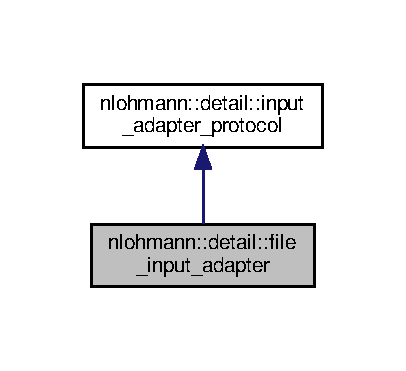
\includegraphics[width=195pt]{classnlohmann_1_1detail_1_1file__input__adapter__inherit__graph}
\end{center}
\end{figure}


Collaboration diagram for nlohmann\+:\+:detail\+:\+:file\+\_\+input\+\_\+adapter\+:
\nopagebreak
\begin{figure}[H]
\begin{center}
\leavevmode
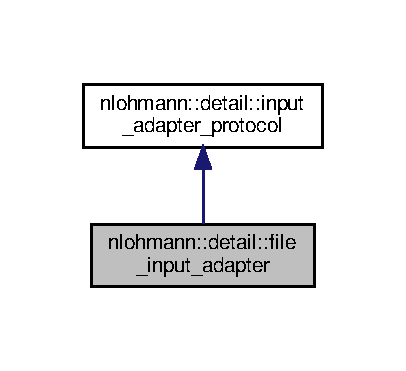
\includegraphics[width=195pt]{classnlohmann_1_1detail_1_1file__input__adapter__coll__graph}
\end{center}
\end{figure}
\subsection*{Public Member Functions}
\begin{DoxyCompactItemize}
\item 
\mbox{\Hypertarget{classnlohmann_1_1detail_1_1file__input__adapter_aeade050f2793280503be93feff2ece5b}\label{classnlohmann_1_1detail_1_1file__input__adapter_aeade050f2793280503be93feff2ece5b}} 
{\bfseries file\+\_\+input\+\_\+adapter} (std\+::\+F\+I\+LE $\ast$f) noexcept
\item 
\mbox{\Hypertarget{classnlohmann_1_1detail_1_1file__input__adapter_a308099b496a0cba2123a06fe99a95d02}\label{classnlohmann_1_1detail_1_1file__input__adapter_a308099b496a0cba2123a06fe99a95d02}} 
{\bfseries file\+\_\+input\+\_\+adapter} (const \hyperlink{classnlohmann_1_1detail_1_1file__input__adapter}{file\+\_\+input\+\_\+adapter} \&)=delete
\item 
\mbox{\Hypertarget{classnlohmann_1_1detail_1_1file__input__adapter_a10b4dec4e8751a4f8a110fa917f0d5a8}\label{classnlohmann_1_1detail_1_1file__input__adapter_a10b4dec4e8751a4f8a110fa917f0d5a8}} 
{\bfseries file\+\_\+input\+\_\+adapter} (\hyperlink{classnlohmann_1_1detail_1_1file__input__adapter}{file\+\_\+input\+\_\+adapter} \&\&)=default
\item 
\mbox{\Hypertarget{classnlohmann_1_1detail_1_1file__input__adapter_ad59bbc7e3f23dd74475c5cb818784e42}\label{classnlohmann_1_1detail_1_1file__input__adapter_ad59bbc7e3f23dd74475c5cb818784e42}} 
\hyperlink{classnlohmann_1_1detail_1_1file__input__adapter}{file\+\_\+input\+\_\+adapter} \& {\bfseries operator=} (const \hyperlink{classnlohmann_1_1detail_1_1file__input__adapter}{file\+\_\+input\+\_\+adapter} \&)=delete
\item 
\mbox{\Hypertarget{classnlohmann_1_1detail_1_1file__input__adapter_a95adaec9a8c583a46083c4c493981e77}\label{classnlohmann_1_1detail_1_1file__input__adapter_a95adaec9a8c583a46083c4c493981e77}} 
\hyperlink{classnlohmann_1_1detail_1_1file__input__adapter}{file\+\_\+input\+\_\+adapter} \& {\bfseries operator=} (\hyperlink{classnlohmann_1_1detail_1_1file__input__adapter}{file\+\_\+input\+\_\+adapter} \&\&)=default
\item 
\mbox{\Hypertarget{classnlohmann_1_1detail_1_1file__input__adapter_a0d4ff48617c8f63c30babdfd09482329}\label{classnlohmann_1_1detail_1_1file__input__adapter_a0d4ff48617c8f63c30babdfd09482329}} 
std\+::char\+\_\+traits$<$ char $>$\+::int\+\_\+type \hyperlink{classnlohmann_1_1detail_1_1file__input__adapter_a0d4ff48617c8f63c30babdfd09482329}{get\+\_\+character} () noexcept override
\begin{DoxyCompactList}\small\item\em get a character \mbox{[}0,255\mbox{]} or std\+::char\+\_\+traits$<$char$>$\+::eof(). \end{DoxyCompactList}\end{DoxyCompactItemize}


\subsection{Detailed Description}
Input adapter for stdio file access. This adapter read only 1 byte and do not use any buffer. This adapter is a very low level adapter. 

The documentation for this class was generated from the following file\+:\begin{DoxyCompactItemize}
\item 
src/tools/json/json.\+hpp\end{DoxyCompactItemize}

\hypertarget{classFlatten}{}\section{Flatten$<$ Value\+Type, Weight\+Type, Data\+Tensor\+Type, Weight\+Tensor\+Type, Converted\+Weights $>$ Class Template Reference}
\label{classFlatten}\index{Flatten$<$ Value\+Type, Weight\+Type, Data\+Tensor\+Type, Weight\+Tensor\+Type, Converted\+Weights $>$@{Flatten$<$ Value\+Type, Weight\+Type, Data\+Tensor\+Type, Weight\+Tensor\+Type, Converted\+Weights $>$}}


Inheritance diagram for Flatten$<$ Value\+Type, Weight\+Type, Data\+Tensor\+Type, Weight\+Tensor\+Type, Converted\+Weights $>$\+:
\nopagebreak
\begin{figure}[H]
\begin{center}
\leavevmode
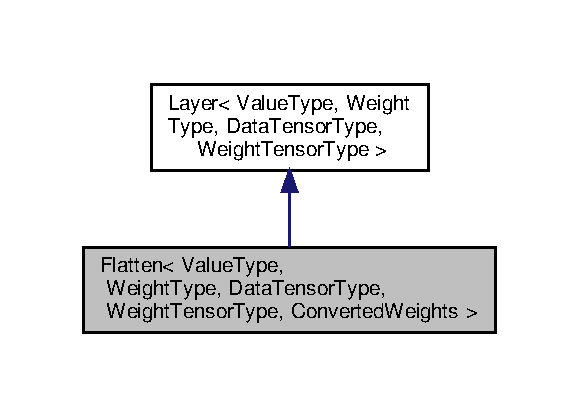
\includegraphics[width=278pt]{classFlatten__inherit__graph}
\end{center}
\end{figure}


Collaboration diagram for Flatten$<$ Value\+Type, Weight\+Type, Data\+Tensor\+Type, Weight\+Tensor\+Type, Converted\+Weights $>$\+:
\nopagebreak
\begin{figure}[H]
\begin{center}
\leavevmode
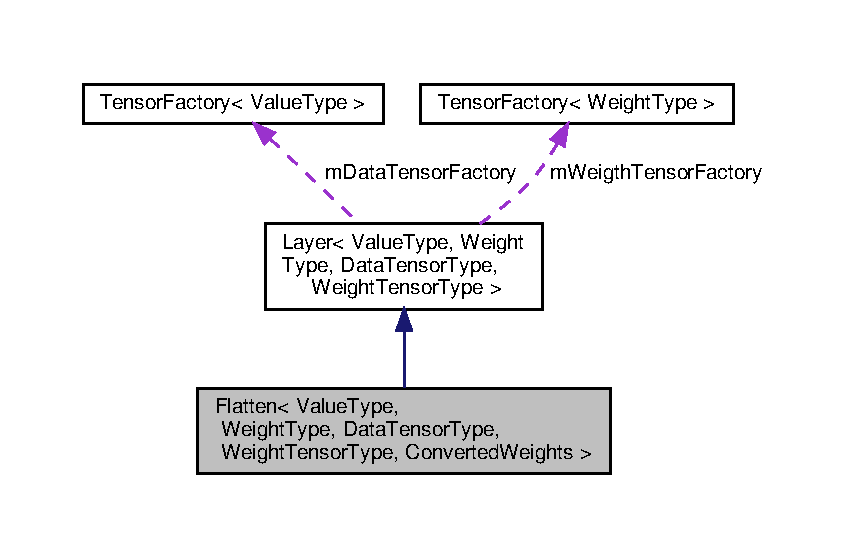
\includegraphics[width=350pt]{classFlatten__coll__graph}
\end{center}
\end{figure}
\subsection*{Public Member Functions}
\begin{DoxyCompactItemize}
\item 
\mbox{\Hypertarget{classFlatten_a5ceaa436f4896997a0867a95c995ae23}\label{classFlatten_a5ceaa436f4896997a0867a95c995ae23}} 
{\bfseries Flatten} (std\+::string name, TensorP$<$ Value\+Type $>$ input, \hyperlink{classTensorFactory}{Tensor\+Factory}$<$ Value\+Type $>$ $\ast$data\+Tensor\+Factory, \hyperlink{classTensorFactory}{Tensor\+Factory}$<$ Weight\+Type $>$ $\ast$weigth\+Tensor\+Factory, bool channels\+First=false)
\item 
\mbox{\Hypertarget{classFlatten_ae9f1c432597e0d7443838fb71a29599e}\label{classFlatten_ae9f1c432597e0d7443838fb71a29599e}} 
{\bfseries Flatten} (std\+::string name, \hyperlink{classTensorFactory}{Tensor\+Factory}$<$ Value\+Type $>$ $\ast$data\+Tensor\+Factory, \hyperlink{classTensorFactory}{Tensor\+Factory}$<$ Weight\+Type $>$ $\ast$weight\+Tensor\+Factory, bool channels\+First=false)
\item 
\mbox{\Hypertarget{classFlatten_a299432e9970733685ded27755243c38b}\label{classFlatten_a299432e9970733685ded27755243c38b}} 
{\bfseries Flatten} (std\+::string name, TensorP$<$ Value\+Type $>$ input, Tensor\+FactoryP$<$ Value\+Type $>$ data\+Tensor\+Factory, Tensor\+FactoryP$<$ Weight\+Type $>$ weight\+Tensor\+Factory, bool channels\+First=false)
\item 
\mbox{\Hypertarget{classFlatten_a0b39a1367b64fc6f1ac5feb4a2729f89}\label{classFlatten_a0b39a1367b64fc6f1ac5feb4a2729f89}} 
{\bfseries Flatten} (std\+::string name, \hyperlink{classTensorFactory}{Tensor\+Factory}$<$ Value\+Type $>$ $\ast$data\+Tensor\+Factory, \hyperlink{classTensorFactory}{Tensor\+Factory}$<$ Weight\+Type $>$ $\ast$weight\+Tensor\+Factory, Tensor\+FactoryP$<$ Value\+Type $>$ dtf, Tensor\+FactoryP$<$ Weight\+Type $>$ wtf, bool channels\+First=false)
\item 
\mbox{\Hypertarget{classFlatten_a11b0e0195b339da71b69f55c97fb39a4}\label{classFlatten_a11b0e0195b339da71b69f55c97fb39a4}} 
{\bfseries Flatten} (std\+::string name, TensorP$<$ Value\+Type $>$ input, bool channels\+First=false)
\item 
\mbox{\Hypertarget{classFlatten_a957a897da50de0eb06450b39323c9616}\label{classFlatten_a957a897da50de0eb06450b39323c9616}} 
{\bfseries Flatten} (std\+::string name, bool channels\+First=false)
\item 
\mbox{\Hypertarget{classFlatten_a263fe8a5f24154851f64fdb64520e40a}\label{classFlatten_a263fe8a5f24154851f64fdb64520e40a}} 
\hyperlink{classShape}{Shape} {\bfseries output\+Shape} () override
\item 
\mbox{\Hypertarget{classFlatten_aed12736c802bdf7cb6b3530f1e581b35}\label{classFlatten_aed12736c802bdf7cb6b3530f1e581b35}} 
void {\bfseries feed\+Forward} () override
\item 
bool \hyperlink{classFlatten_a53379945e182152effef9456b32eb65a}{builds\+Own\+Output\+Tensor} () override
\begin{DoxyCompactList}\small\item\em This function is supposed to be used if a layer needs to build a special output layer. It will get called when layers gets added to the model. Build yuour own output layer in this function and return false. \end{DoxyCompactList}\item 
\mbox{\Hypertarget{classFlatten_aa24e68c4f410565483161c7214556d9d}\label{classFlatten_aa24e68c4f410565483161c7214556d9d}} 
void {\bfseries load\+Weights} (std\+::string path, std\+::string file\+Name)
\item 
\mbox{\Hypertarget{classFlatten_a0eee4c2e4f98bf2a4d19b9283b8f47f7}\label{classFlatten_a0eee4c2e4f98bf2a4d19b9283b8f47f7}} 
void {\bfseries load\+Weights} (std\+::string path)
\item 
\mbox{\Hypertarget{classFlatten_a4c95c3512c62bc6e82d13515447515f8}\label{classFlatten_a4c95c3512c62bc6e82d13515447515f8}} 
virtual void {\bfseries random\+Init} () override
\item 
\mbox{\Hypertarget{classFlatten_a8c35a22fe96db562180199193cc79b5c}\label{classFlatten_a8c35a22fe96db562180199193cc79b5c}} 
void {\bfseries description} () override
\item 
\mbox{\Hypertarget{classFlatten_ac7d8cd2d0e206e1cacb71e66ec4ec3e3}\label{classFlatten_ac7d8cd2d0e206e1cacb71e66ec4ec3e3}} 
virtual std\+::vector$<$ TensorP$<$ Weight\+Type $>$ $>$ \hyperlink{classFlatten_ac7d8cd2d0e206e1cacb71e66ec4ec3e3}{all\+Weights} () override
\begin{DoxyCompactList}\small\item\em Returns empty vector. \end{DoxyCompactList}\end{DoxyCompactItemize}
\subsection*{Additional Inherited Members}


\subsection{Member Function Documentation}
\mbox{\Hypertarget{classFlatten_a53379945e182152effef9456b32eb65a}\label{classFlatten_a53379945e182152effef9456b32eb65a}} 
\index{Flatten@{Flatten}!builds\+Own\+Output\+Tensor@{builds\+Own\+Output\+Tensor}}
\index{builds\+Own\+Output\+Tensor@{builds\+Own\+Output\+Tensor}!Flatten@{Flatten}}
\subsubsection{\texorpdfstring{builds\+Own\+Output\+Tensor()}{buildsOwnOutputTensor()}}
{\footnotesize\ttfamily template$<$class Value\+Type , class Weight\+Type , class Data\+Tensor\+Type  = Tensor\+P$<$\+Value\+Type$>$, class Weight\+Tensor\+Type  = Tensor\+P$<$\+Weight\+Type$>$, class Converted\+Weights  = float$>$ \\
bool \hyperlink{classFlatten}{Flatten}$<$ Value\+Type, Weight\+Type, Data\+Tensor\+Type, Weight\+Tensor\+Type, Converted\+Weights $>$\+::builds\+Own\+Output\+Tensor (\begin{DoxyParamCaption}{ }\end{DoxyParamCaption})\hspace{0.3cm}{\ttfamily [inline]}, {\ttfamily [override]}, {\ttfamily [virtual]}}



This function is supposed to be used if a layer needs to build a special output layer. It will get called when layers gets added to the model. Build yuour own output layer in this function and return false. 

See \hyperlink{classFlatten}{Flatten} for an example 

Reimplemented from \hyperlink{classLayer_a9a126cb372c0bd529c65a06077d8b429}{Layer$<$ Value\+Type, Weight\+Type, Data\+Tensor\+Type, Weight\+Tensor\+Type $>$}.



The documentation for this class was generated from the following file\+:\begin{DoxyCompactItemize}
\item 
src/architecture/Layer\+Impl.\+h\end{DoxyCompactItemize}

\hypertarget{structnlohmann_1_1detail_1_1from__json__fn}{}\section{nlohmann\+:\+:detail\+:\+:from\+\_\+json\+\_\+fn Struct Reference}
\label{structnlohmann_1_1detail_1_1from__json__fn}\index{nlohmann\+::detail\+::from\+\_\+json\+\_\+fn@{nlohmann\+::detail\+::from\+\_\+json\+\_\+fn}}
\subsection*{Public Member Functions}
\begin{DoxyCompactItemize}
\item 
\mbox{\Hypertarget{structnlohmann_1_1detail_1_1from__json__fn_a6d14a74e1043072c77892534572d2973}\label{structnlohmann_1_1detail_1_1from__json__fn_a6d14a74e1043072c77892534572d2973}} 
{\footnotesize template$<$typename Basic\+Json\+Type , typename T $>$ }\\auto {\bfseries operator()} (const Basic\+Json\+Type \&j, T \&val) const noexcept(noexcept(from\+\_\+json(j, val))) -\/$>$ decltype(from\+\_\+json(j, val), void())
\end{DoxyCompactItemize}


The documentation for this struct was generated from the following file\+:\begin{DoxyCompactItemize}
\item 
src/tools/json/json.\+hpp\end{DoxyCompactItemize}

\hypertarget{structnlohmann_1_1detail_1_1has__from__json}{}\section{nlohmann\+:\+:detail\+:\+:has\+\_\+from\+\_\+json$<$ Basic\+Json\+Type, T, typename $>$ Struct Template Reference}
\label{structnlohmann_1_1detail_1_1has__from__json}\index{nlohmann\+::detail\+::has\+\_\+from\+\_\+json$<$ Basic\+Json\+Type, T, typename $>$@{nlohmann\+::detail\+::has\+\_\+from\+\_\+json$<$ Basic\+Json\+Type, T, typename $>$}}


Inheritance diagram for nlohmann\+:\+:detail\+:\+:has\+\_\+from\+\_\+json$<$ Basic\+Json\+Type, T, typename $>$\+:
\nopagebreak
\begin{figure}[H]
\begin{center}
\leavevmode
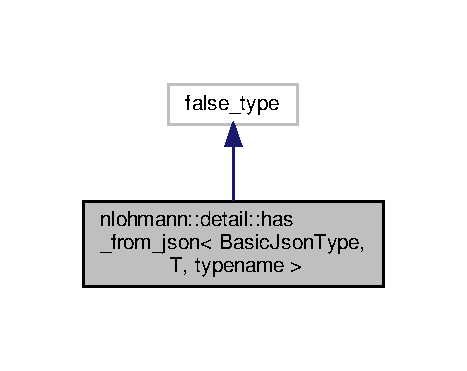
\includegraphics[width=224pt]{structnlohmann_1_1detail_1_1has__from__json__inherit__graph}
\end{center}
\end{figure}


Collaboration diagram for nlohmann\+:\+:detail\+:\+:has\+\_\+from\+\_\+json$<$ Basic\+Json\+Type, T, typename $>$\+:
\nopagebreak
\begin{figure}[H]
\begin{center}
\leavevmode
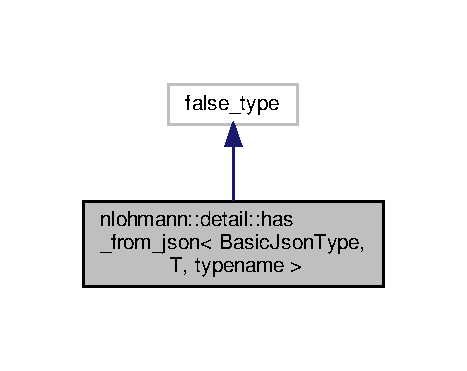
\includegraphics[width=224pt]{structnlohmann_1_1detail_1_1has__from__json__coll__graph}
\end{center}
\end{figure}


The documentation for this struct was generated from the following file\+:\begin{DoxyCompactItemize}
\item 
src/tools/json/json.\+hpp\end{DoxyCompactItemize}

\hypertarget{structnlohmann_1_1detail_1_1has__from__json_3_01BasicJsonType_00_01T_00_01enable__if__t_3_01not_5e786a91cad76ed1c14f425887b41640}{}\section{nlohmann\+:\+:detail\+:\+:has\+\_\+from\+\_\+json$<$ Basic\+Json\+Type, T, enable\+\_\+if\+\_\+t$<$ not is\+\_\+basic\+\_\+json$<$ T $>$\+:\+:value $>$ $>$ Struct Template Reference}
\label{structnlohmann_1_1detail_1_1has__from__json_3_01BasicJsonType_00_01T_00_01enable__if__t_3_01not_5e786a91cad76ed1c14f425887b41640}\index{nlohmann\+::detail\+::has\+\_\+from\+\_\+json$<$ Basic\+Json\+Type, T, enable\+\_\+if\+\_\+t$<$ not is\+\_\+basic\+\_\+json$<$ T $>$\+::value $>$ $>$@{nlohmann\+::detail\+::has\+\_\+from\+\_\+json$<$ Basic\+Json\+Type, T, enable\+\_\+if\+\_\+t$<$ not is\+\_\+basic\+\_\+json$<$ T $>$\+::value $>$ $>$}}
\subsection*{Public Types}
\begin{DoxyCompactItemize}
\item 
\mbox{\Hypertarget{structnlohmann_1_1detail_1_1has__from__json_3_01BasicJsonType_00_01T_00_01enable__if__t_3_01not_5e786a91cad76ed1c14f425887b41640_ab17cea1be422b8985fc19942809560ed}\label{structnlohmann_1_1detail_1_1has__from__json_3_01BasicJsonType_00_01T_00_01enable__if__t_3_01not_5e786a91cad76ed1c14f425887b41640_ab17cea1be422b8985fc19942809560ed}} 
using {\bfseries serializer} = typename Basic\+Json\+Type\+::template json\+\_\+serializer$<$ T, void $>$
\end{DoxyCompactItemize}
\subsection*{Static Public Attributes}
\begin{DoxyCompactItemize}
\item 
static constexpr bool {\bfseries value}
\end{DoxyCompactItemize}


\subsection{Member Data Documentation}
\mbox{\Hypertarget{structnlohmann_1_1detail_1_1has__from__json_3_01BasicJsonType_00_01T_00_01enable__if__t_3_01not_5e786a91cad76ed1c14f425887b41640_afb638d592883301228bcad21d83bf4aa}\label{structnlohmann_1_1detail_1_1has__from__json_3_01BasicJsonType_00_01T_00_01enable__if__t_3_01not_5e786a91cad76ed1c14f425887b41640_afb638d592883301228bcad21d83bf4aa}} 
\index{nlohmann\+::detail\+::has\+\_\+from\+\_\+json$<$ Basic\+Json\+Type, T, enable\+\_\+if\+\_\+t$<$ not is\+\_\+basic\+\_\+json$<$ T $>$\+::value $>$ $>$@{nlohmann\+::detail\+::has\+\_\+from\+\_\+json$<$ Basic\+Json\+Type, T, enable\+\_\+if\+\_\+t$<$ not is\+\_\+basic\+\_\+json$<$ T $>$\+::value $>$ $>$}!value@{value}}
\index{value@{value}!nlohmann\+::detail\+::has\+\_\+from\+\_\+json$<$ Basic\+Json\+Type, T, enable\+\_\+if\+\_\+t$<$ not is\+\_\+basic\+\_\+json$<$ T $>$\+::value $>$ $>$@{nlohmann\+::detail\+::has\+\_\+from\+\_\+json$<$ Basic\+Json\+Type, T, enable\+\_\+if\+\_\+t$<$ not is\+\_\+basic\+\_\+json$<$ T $>$\+::value $>$ $>$}}
\subsubsection{\texorpdfstring{value}{value}}
{\footnotesize\ttfamily template$<$typename Basic\+Json\+Type , typename T $>$ \\
constexpr bool \hyperlink{structnlohmann_1_1detail_1_1has__from__json}{nlohmann\+::detail\+::has\+\_\+from\+\_\+json}$<$ Basic\+Json\+Type, T, enable\+\_\+if\+\_\+t$<$ not \hyperlink{structnlohmann_1_1detail_1_1is__basic__json}{is\+\_\+basic\+\_\+json}$<$ T $>$\+::value $>$ $>$\+::value\hspace{0.3cm}{\ttfamily [static]}}

{\bfseries Initial value\+:}
\begin{DoxyCode}
=
        is\_detected\_exact<void, from\_json\_function, serializer,
        \textcolor{keyword}{const} BasicJsonType&, T&>::value
\end{DoxyCode}


The documentation for this struct was generated from the following file\+:\begin{DoxyCompactItemize}
\item 
src/tools/json/json.\+hpp\end{DoxyCompactItemize}

\hypertarget{structnlohmann_1_1detail_1_1has__non__default__from__json}{}\section{nlohmann\+:\+:detail\+:\+:has\+\_\+non\+\_\+default\+\_\+from\+\_\+json$<$ Basic\+Json\+Type, T, typename $>$ Struct Template Reference}
\label{structnlohmann_1_1detail_1_1has__non__default__from__json}\index{nlohmann\+::detail\+::has\+\_\+non\+\_\+default\+\_\+from\+\_\+json$<$ Basic\+Json\+Type, T, typename $>$@{nlohmann\+::detail\+::has\+\_\+non\+\_\+default\+\_\+from\+\_\+json$<$ Basic\+Json\+Type, T, typename $>$}}


Inheritance diagram for nlohmann\+:\+:detail\+:\+:has\+\_\+non\+\_\+default\+\_\+from\+\_\+json$<$ Basic\+Json\+Type, T, typename $>$\+:
\nopagebreak
\begin{figure}[H]
\begin{center}
\leavevmode
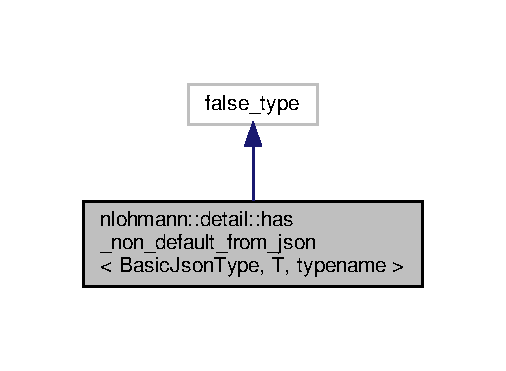
\includegraphics[width=243pt]{structnlohmann_1_1detail_1_1has__non__default__from__json__inherit__graph}
\end{center}
\end{figure}


Collaboration diagram for nlohmann\+:\+:detail\+:\+:has\+\_\+non\+\_\+default\+\_\+from\+\_\+json$<$ Basic\+Json\+Type, T, typename $>$\+:
\nopagebreak
\begin{figure}[H]
\begin{center}
\leavevmode
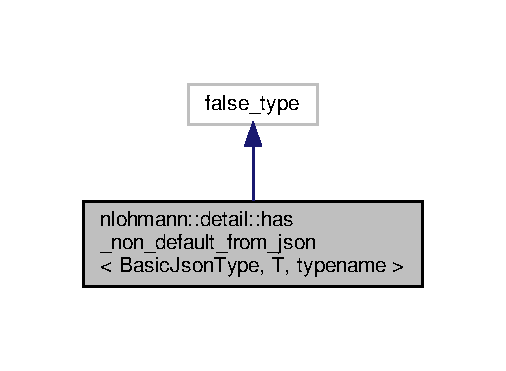
\includegraphics[width=243pt]{structnlohmann_1_1detail_1_1has__non__default__from__json__coll__graph}
\end{center}
\end{figure}


The documentation for this struct was generated from the following file\+:\begin{DoxyCompactItemize}
\item 
src/tools/json/json.\+hpp\end{DoxyCompactItemize}

\hypertarget{structnlohmann_1_1detail_1_1has__non__default__from__json_3_01BasicJsonType_00_01T_00_01enable__a9e4562f31f7ed523e6e0f675606b0f2}{}\section{nlohmann\+:\+:detail\+:\+:has\+\_\+non\+\_\+default\+\_\+from\+\_\+json$<$ Basic\+Json\+Type, T, enable\+\_\+if\+\_\+t$<$ not is\+\_\+basic\+\_\+json$<$ T $>$\+:\+:value $>$ $>$ Struct Template Reference}
\label{structnlohmann_1_1detail_1_1has__non__default__from__json_3_01BasicJsonType_00_01T_00_01enable__a9e4562f31f7ed523e6e0f675606b0f2}\index{nlohmann\+::detail\+::has\+\_\+non\+\_\+default\+\_\+from\+\_\+json$<$ Basic\+Json\+Type, T, enable\+\_\+if\+\_\+t$<$ not is\+\_\+basic\+\_\+json$<$ T $>$\+::value $>$ $>$@{nlohmann\+::detail\+::has\+\_\+non\+\_\+default\+\_\+from\+\_\+json$<$ Basic\+Json\+Type, T, enable\+\_\+if\+\_\+t$<$ not is\+\_\+basic\+\_\+json$<$ T $>$\+::value $>$ $>$}}
\subsection*{Public Types}
\begin{DoxyCompactItemize}
\item 
\mbox{\Hypertarget{structnlohmann_1_1detail_1_1has__non__default__from__json_3_01BasicJsonType_00_01T_00_01enable__a9e4562f31f7ed523e6e0f675606b0f2_a610272ed924122e0c46d158ecdfe6faf}\label{structnlohmann_1_1detail_1_1has__non__default__from__json_3_01BasicJsonType_00_01T_00_01enable__a9e4562f31f7ed523e6e0f675606b0f2_a610272ed924122e0c46d158ecdfe6faf}} 
using {\bfseries serializer} = typename Basic\+Json\+Type\+::template json\+\_\+serializer$<$ T, void $>$
\end{DoxyCompactItemize}
\subsection*{Static Public Attributes}
\begin{DoxyCompactItemize}
\item 
static constexpr bool {\bfseries value}
\end{DoxyCompactItemize}


\subsection{Member Data Documentation}
\mbox{\Hypertarget{structnlohmann_1_1detail_1_1has__non__default__from__json_3_01BasicJsonType_00_01T_00_01enable__a9e4562f31f7ed523e6e0f675606b0f2_a1494ac5fed1163aab4a89208ff04ee85}\label{structnlohmann_1_1detail_1_1has__non__default__from__json_3_01BasicJsonType_00_01T_00_01enable__a9e4562f31f7ed523e6e0f675606b0f2_a1494ac5fed1163aab4a89208ff04ee85}} 
\index{nlohmann\+::detail\+::has\+\_\+non\+\_\+default\+\_\+from\+\_\+json$<$ Basic\+Json\+Type, T, enable\+\_\+if\+\_\+t$<$ not is\+\_\+basic\+\_\+json$<$ T $>$\+::value $>$ $>$@{nlohmann\+::detail\+::has\+\_\+non\+\_\+default\+\_\+from\+\_\+json$<$ Basic\+Json\+Type, T, enable\+\_\+if\+\_\+t$<$ not is\+\_\+basic\+\_\+json$<$ T $>$\+::value $>$ $>$}!value@{value}}
\index{value@{value}!nlohmann\+::detail\+::has\+\_\+non\+\_\+default\+\_\+from\+\_\+json$<$ Basic\+Json\+Type, T, enable\+\_\+if\+\_\+t$<$ not is\+\_\+basic\+\_\+json$<$ T $>$\+::value $>$ $>$@{nlohmann\+::detail\+::has\+\_\+non\+\_\+default\+\_\+from\+\_\+json$<$ Basic\+Json\+Type, T, enable\+\_\+if\+\_\+t$<$ not is\+\_\+basic\+\_\+json$<$ T $>$\+::value $>$ $>$}}
\subsubsection{\texorpdfstring{value}{value}}
{\footnotesize\ttfamily template$<$typename Basic\+Json\+Type , typename T $>$ \\
constexpr bool \hyperlink{structnlohmann_1_1detail_1_1has__non__default__from__json}{nlohmann\+::detail\+::has\+\_\+non\+\_\+default\+\_\+from\+\_\+json}$<$ Basic\+Json\+Type, T, enable\+\_\+if\+\_\+t$<$ not \hyperlink{structnlohmann_1_1detail_1_1is__basic__json}{is\+\_\+basic\+\_\+json}$<$ T $>$\+::value $>$ $>$\+::value\hspace{0.3cm}{\ttfamily [static]}}

{\bfseries Initial value\+:}
\begin{DoxyCode}
=
        is\_detected\_exact<T, from\_json\_function, serializer,
        \textcolor{keyword}{const} BasicJsonType&>::value
\end{DoxyCode}


The documentation for this struct was generated from the following file\+:\begin{DoxyCompactItemize}
\item 
src/tools/json/json.\+hpp\end{DoxyCompactItemize}

\hypertarget{structnlohmann_1_1detail_1_1has__to__json}{}\section{nlohmann\+:\+:detail\+:\+:has\+\_\+to\+\_\+json$<$ Basic\+Json\+Type, T, typename $>$ Struct Template Reference}
\label{structnlohmann_1_1detail_1_1has__to__json}\index{nlohmann\+::detail\+::has\+\_\+to\+\_\+json$<$ Basic\+Json\+Type, T, typename $>$@{nlohmann\+::detail\+::has\+\_\+to\+\_\+json$<$ Basic\+Json\+Type, T, typename $>$}}


Inheritance diagram for nlohmann\+:\+:detail\+:\+:has\+\_\+to\+\_\+json$<$ Basic\+Json\+Type, T, typename $>$\+:
\nopagebreak
\begin{figure}[H]
\begin{center}
\leavevmode
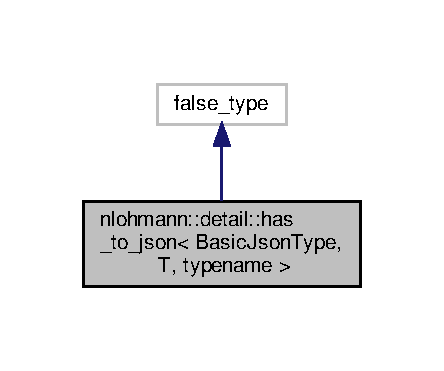
\includegraphics[width=213pt]{structnlohmann_1_1detail_1_1has__to__json__inherit__graph}
\end{center}
\end{figure}


Collaboration diagram for nlohmann\+:\+:detail\+:\+:has\+\_\+to\+\_\+json$<$ Basic\+Json\+Type, T, typename $>$\+:
\nopagebreak
\begin{figure}[H]
\begin{center}
\leavevmode
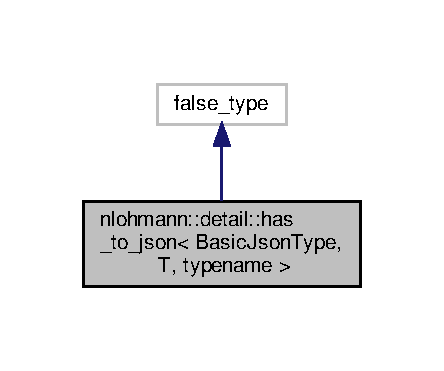
\includegraphics[width=213pt]{structnlohmann_1_1detail_1_1has__to__json__coll__graph}
\end{center}
\end{figure}


The documentation for this struct was generated from the following file\+:\begin{DoxyCompactItemize}
\item 
src/tools/json/json.\+hpp\end{DoxyCompactItemize}

\hypertarget{structnlohmann_1_1detail_1_1has__to__json_3_01BasicJsonType_00_01T_00_01enable__if__t_3_01not_01737900a749c335e922e2f74e2face5e4}{}\section{nlohmann\+:\+:detail\+:\+:has\+\_\+to\+\_\+json$<$ Basic\+Json\+Type, T, enable\+\_\+if\+\_\+t$<$ not is\+\_\+basic\+\_\+json$<$ T $>$\+:\+:value $>$ $>$ Struct Template Reference}
\label{structnlohmann_1_1detail_1_1has__to__json_3_01BasicJsonType_00_01T_00_01enable__if__t_3_01not_01737900a749c335e922e2f74e2face5e4}\index{nlohmann\+::detail\+::has\+\_\+to\+\_\+json$<$ Basic\+Json\+Type, T, enable\+\_\+if\+\_\+t$<$ not is\+\_\+basic\+\_\+json$<$ T $>$\+::value $>$ $>$@{nlohmann\+::detail\+::has\+\_\+to\+\_\+json$<$ Basic\+Json\+Type, T, enable\+\_\+if\+\_\+t$<$ not is\+\_\+basic\+\_\+json$<$ T $>$\+::value $>$ $>$}}
\subsection*{Public Types}
\begin{DoxyCompactItemize}
\item 
\mbox{\Hypertarget{structnlohmann_1_1detail_1_1has__to__json_3_01BasicJsonType_00_01T_00_01enable__if__t_3_01not_01737900a749c335e922e2f74e2face5e4_a479098e9480e0adb30fb3fe3586a8005}\label{structnlohmann_1_1detail_1_1has__to__json_3_01BasicJsonType_00_01T_00_01enable__if__t_3_01not_01737900a749c335e922e2f74e2face5e4_a479098e9480e0adb30fb3fe3586a8005}} 
using {\bfseries serializer} = typename Basic\+Json\+Type\+::template json\+\_\+serializer$<$ T, void $>$
\end{DoxyCompactItemize}
\subsection*{Static Public Attributes}
\begin{DoxyCompactItemize}
\item 
static constexpr bool {\bfseries value}
\end{DoxyCompactItemize}


\subsection{Member Data Documentation}
\mbox{\Hypertarget{structnlohmann_1_1detail_1_1has__to__json_3_01BasicJsonType_00_01T_00_01enable__if__t_3_01not_01737900a749c335e922e2f74e2face5e4_ac5e2f95bd9fa54c6ea870e923e395b63}\label{structnlohmann_1_1detail_1_1has__to__json_3_01BasicJsonType_00_01T_00_01enable__if__t_3_01not_01737900a749c335e922e2f74e2face5e4_ac5e2f95bd9fa54c6ea870e923e395b63}} 
\index{nlohmann\+::detail\+::has\+\_\+to\+\_\+json$<$ Basic\+Json\+Type, T, enable\+\_\+if\+\_\+t$<$ not is\+\_\+basic\+\_\+json$<$ T $>$\+::value $>$ $>$@{nlohmann\+::detail\+::has\+\_\+to\+\_\+json$<$ Basic\+Json\+Type, T, enable\+\_\+if\+\_\+t$<$ not is\+\_\+basic\+\_\+json$<$ T $>$\+::value $>$ $>$}!value@{value}}
\index{value@{value}!nlohmann\+::detail\+::has\+\_\+to\+\_\+json$<$ Basic\+Json\+Type, T, enable\+\_\+if\+\_\+t$<$ not is\+\_\+basic\+\_\+json$<$ T $>$\+::value $>$ $>$@{nlohmann\+::detail\+::has\+\_\+to\+\_\+json$<$ Basic\+Json\+Type, T, enable\+\_\+if\+\_\+t$<$ not is\+\_\+basic\+\_\+json$<$ T $>$\+::value $>$ $>$}}
\subsubsection{\texorpdfstring{value}{value}}
{\footnotesize\ttfamily template$<$typename Basic\+Json\+Type , typename T $>$ \\
constexpr bool \hyperlink{structnlohmann_1_1detail_1_1has__to__json}{nlohmann\+::detail\+::has\+\_\+to\+\_\+json}$<$ Basic\+Json\+Type, T, enable\+\_\+if\+\_\+t$<$ not \hyperlink{structnlohmann_1_1detail_1_1is__basic__json}{is\+\_\+basic\+\_\+json}$<$ T $>$\+::value $>$ $>$\+::value\hspace{0.3cm}{\ttfamily [static]}}

{\bfseries Initial value\+:}
\begin{DoxyCode}
=
        is\_detected\_exact<void, to\_json\_function, serializer, BasicJsonType&,
        T>::value
\end{DoxyCode}


The documentation for this struct was generated from the following file\+:\begin{DoxyCompactItemize}
\item 
src/tools/json/json.\+hpp\end{DoxyCompactItemize}

\hypertarget{structstd_1_1hash_3_01nlohmann_1_1json_01_4}{}\section{std\+:\+:hash$<$ nlohmann\+:\+:json $>$ Struct Template Reference}
\label{structstd_1_1hash_3_01nlohmann_1_1json_01_4}\index{std\+::hash$<$ nlohmann\+::json $>$@{std\+::hash$<$ nlohmann\+::json $>$}}


hash value for J\+S\+ON objects  




{\ttfamily \#include $<$json.\+hpp$>$}

\subsection*{Public Member Functions}
\begin{DoxyCompactItemize}
\item 
std\+::size\+\_\+t \hyperlink{structstd_1_1hash_3_01nlohmann_1_1json_01_4_aec1567d1fa47dbe5b77954dce3a55b64}{operator()} (const \hyperlink{namespacenlohmann_a2bfd99e845a2e5cd90aeaf1b1431f474}{nlohmann\+::json} \&j) const
\begin{DoxyCompactList}\small\item\em return a hash value for a J\+S\+ON object \end{DoxyCompactList}\end{DoxyCompactItemize}


\subsection{Detailed Description}
\subsubsection*{template$<$$>$\newline
struct std\+::hash$<$ nlohmann\+::json $>$}

hash value for J\+S\+ON objects 

\subsection{Member Function Documentation}
\mbox{\Hypertarget{structstd_1_1hash_3_01nlohmann_1_1json_01_4_aec1567d1fa47dbe5b77954dce3a55b64}\label{structstd_1_1hash_3_01nlohmann_1_1json_01_4_aec1567d1fa47dbe5b77954dce3a55b64}} 
\index{std\+::hash$<$ nlohmann\+::json $>$@{std\+::hash$<$ nlohmann\+::json $>$}!operator()@{operator()}}
\index{operator()@{operator()}!std\+::hash$<$ nlohmann\+::json $>$@{std\+::hash$<$ nlohmann\+::json $>$}}
\subsubsection{\texorpdfstring{operator()()}{operator()()}}
{\footnotesize\ttfamily std\+::size\+\_\+t std\+::hash$<$ \hyperlink{namespacenlohmann_a2bfd99e845a2e5cd90aeaf1b1431f474}{nlohmann\+::json} $>$\+::operator() (\begin{DoxyParamCaption}\item[{const \hyperlink{namespacenlohmann_a2bfd99e845a2e5cd90aeaf1b1431f474}{nlohmann\+::json} \&}]{j }\end{DoxyParamCaption}) const\hspace{0.3cm}{\ttfamily [inline]}}



return a hash value for a J\+S\+ON object 

\begin{DoxySince}{Since}
version 1.\+0.\+0 
\end{DoxySince}


The documentation for this struct was generated from the following file\+:\begin{DoxyCompactItemize}
\item 
src/tools/json/json.\+hpp\end{DoxyCompactItemize}

\hypertarget{classHELibCipherText}{}\section{H\+E\+Lib\+Cipher\+Text Class Reference}
\label{classHELibCipherText}\index{H\+E\+Lib\+Cipher\+Text@{H\+E\+Lib\+Cipher\+Text}}


Collaboration diagram for H\+E\+Lib\+Cipher\+Text\+:
\nopagebreak
\begin{figure}[H]
\begin{center}
\leavevmode
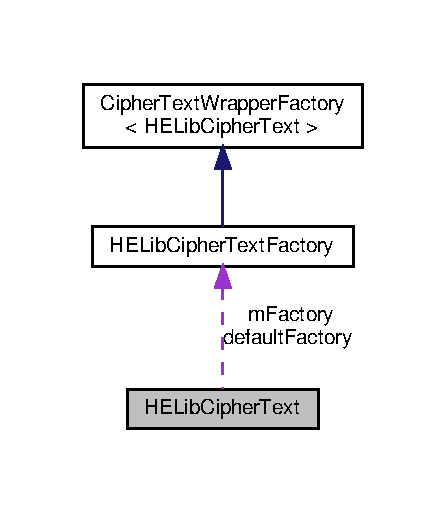
\includegraphics[width=214pt]{classHELibCipherText__coll__graph}
\end{center}
\end{figure}
\subsection*{Public Member Functions}
\begin{DoxyCompactItemize}
\item 
\mbox{\Hypertarget{classHELibCipherText_abd011478fe2945c0feec8eff1fa317f1}\label{classHELibCipherText_abd011478fe2945c0feec8eff1fa317f1}} 
{\bfseries H\+E\+Lib\+Cipher\+Text} (std\+::shared\+\_\+ptr$<$ Ctxt $>$ ctxt, \hyperlink{classHELibCipherTextFactory}{H\+E\+Lib\+Cipher\+Text\+Factory} $\ast$factory)
\item 
\mbox{\Hypertarget{classHELibCipherText_a62abdb390c87479c5f622570fd7b5f8b}\label{classHELibCipherText_a62abdb390c87479c5f622570fd7b5f8b}} 
const Ctxt \& {\bfseries ctxt} () const
\item 
\mbox{\Hypertarget{classHELibCipherText_a186826b8e297a2587f0b5ddc9567cde4}\label{classHELibCipherText_a186826b8e297a2587f0b5ddc9567cde4}} 
virtual \hyperlink{classHELibCipherText}{H\+E\+Lib\+Cipher\+Text} \& {\bfseries operator+=} (long x)
\item 
\mbox{\Hypertarget{classHELibCipherText_ad36eb42b8d0208fc5903fe9f2969ffa3}\label{classHELibCipherText_ad36eb42b8d0208fc5903fe9f2969ffa3}} 
virtual \hyperlink{classHELibCipherText}{H\+E\+Lib\+Cipher\+Text} \& {\bfseries operator$\ast$=} (long x)
\item 
\mbox{\Hypertarget{classHELibCipherText_a747f98ae50587783a2192618701bbc8c}\label{classHELibCipherText_a747f98ae50587783a2192618701bbc8c}} 
virtual \hyperlink{classHELibCipherText}{H\+E\+Lib\+Cipher\+Text} \& {\bfseries operator+=} (float x)
\item 
\mbox{\Hypertarget{classHELibCipherText_af8e5454f98c8af7fdd5bbf9d96428f31}\label{classHELibCipherText_af8e5454f98c8af7fdd5bbf9d96428f31}} 
virtual \hyperlink{classHELibCipherText}{H\+E\+Lib\+Cipher\+Text} \& {\bfseries operator$\ast$=} (float x)
\item 
\mbox{\Hypertarget{classHELibCipherText_aa0460b1883958db2e30c638a8192ceb5}\label{classHELibCipherText_aa0460b1883958db2e30c638a8192ceb5}} 
virtual \hyperlink{classHELibCipherText}{H\+E\+Lib\+Cipher\+Text} \& {\bfseries operator+=} (double x)
\item 
\mbox{\Hypertarget{classHELibCipherText_a4244fa5db6b3ce11b420e18acb3be763}\label{classHELibCipherText_a4244fa5db6b3ce11b420e18acb3be763}} 
virtual \hyperlink{classHELibCipherText}{H\+E\+Lib\+Cipher\+Text} \& {\bfseries operator$\ast$=} (double x)
\item 
\mbox{\Hypertarget{classHELibCipherText_ae27121fd664b3035d439df0dcc1a260f}\label{classHELibCipherText_ae27121fd664b3035d439df0dcc1a260f}} 
virtual \hyperlink{classHELibCipherText}{H\+E\+Lib\+Cipher\+Text} \& {\bfseries operator+=} (\hyperlink{classHELibCipherText}{H\+E\+Lib\+Cipher\+Text} $\ast$other)
\item 
\mbox{\Hypertarget{classHELibCipherText_ab6377e4bf0d41afdf197a1a5d71e962a}\label{classHELibCipherText_ab6377e4bf0d41afdf197a1a5d71e962a}} 
virtual \hyperlink{classHELibCipherText}{H\+E\+Lib\+Cipher\+Text} \& {\bfseries operator$\ast$=} (\hyperlink{classHELibCipherText}{H\+E\+Lib\+Cipher\+Text} $\ast$other)
\item 
\mbox{\Hypertarget{classHELibCipherText_a4e7fa1f2a1ea50b93ce11b4b4f8c2e03}\label{classHELibCipherText_a4e7fa1f2a1ea50b93ce11b4b4f8c2e03}} 
virtual \hyperlink{classHELibCipherText}{H\+E\+Lib\+Cipher\+Text} \& {\bfseries operator+=} (\hyperlink{classHELibCipherText}{H\+E\+Lib\+Cipher\+Text} \&other)
\item 
\mbox{\Hypertarget{classHELibCipherText_a716cb0493c84fa579f4832af4a526aa3}\label{classHELibCipherText_a716cb0493c84fa579f4832af4a526aa3}} 
virtual \hyperlink{classHELibCipherText}{H\+E\+Lib\+Cipher\+Text} \& {\bfseries operator$\ast$=} (\hyperlink{classHELibCipherText}{H\+E\+Lib\+Cipher\+Text} \&other)
\item 
\mbox{\Hypertarget{classHELibCipherText_a1c15638ff87af1b47284bd989f1d5ae8}\label{classHELibCipherText_a1c15638ff87af1b47284bd989f1d5ae8}} 
virtual \hyperlink{classHELibCipherText}{H\+E\+Lib\+Cipher\+Text} {\bfseries empty} ()
\item 
\mbox{\Hypertarget{classHELibCipherText_a5f22ca53fc9eecbe4832a1825a5de743}\label{classHELibCipherText_a5f22ca53fc9eecbe4832a1825a5de743}} 
void {\bfseries square} ()
\item 
\mbox{\Hypertarget{classHELibCipherText_ad54baf34b1a02a1d612c06fc4161a8ee}\label{classHELibCipherText_ad54baf34b1a02a1d612c06fc4161a8ee}} 
void {\bfseries power} (uint p)
\item 
\mbox{\Hypertarget{classHELibCipherText_ad55e5d6fa479d459ffc9e55232e511f5}\label{classHELibCipherText_ad55e5d6fa479d459ffc9e55232e511f5}} 
bool \hyperlink{classHELibCipherText_ad55e5d6fa479d459ffc9e55232e511f5}{noise\+Near\+Overflow} ()
\begin{DoxyCompactList}\small\item\em Checks if the noise is about to overflow. \end{DoxyCompactList}\end{DoxyCompactItemize}
\subsection*{Public Attributes}
\begin{DoxyCompactItemize}
\item 
\mbox{\Hypertarget{classHELibCipherText_a381d85c9c460b5003e2f81f2f7e9480b}\label{classHELibCipherText_a381d85c9c460b5003e2f81f2f7e9480b}} 
friend {\bfseries H\+E\+Lib\+Cipher\+Text\+Factory}
\item 
\mbox{\Hypertarget{classHELibCipherText_abf2e204089bb5428c5710468f3c1025b}\label{classHELibCipherText_abf2e204089bb5428c5710468f3c1025b}} 
\hyperlink{classHELibCipherTextFactory}{H\+E\+Lib\+Cipher\+Text\+Factory} $\ast$ {\bfseries m\+Factory}
\item 
\mbox{\Hypertarget{classHELibCipherText_ac3bb6aa6de466df9bc2bf428dfb8d17d}\label{classHELibCipherText_ac3bb6aa6de466df9bc2bf428dfb8d17d}} 
std\+::shared\+\_\+ptr$<$ Ctxt $>$ {\bfseries m\+Ctxt}
\end{DoxyCompactItemize}
\subsection*{Static Public Attributes}
\begin{DoxyCompactItemize}
\item 
\mbox{\Hypertarget{classHELibCipherText_aa69789ae95ec28a396e6b814841b6b96}\label{classHELibCipherText_aa69789ae95ec28a396e6b814841b6b96}} 
static \hyperlink{classHELibCipherTextFactory}{H\+E\+Lib\+Cipher\+Text\+Factory} $\ast$ {\bfseries default\+Factory} = nullptr
\item 
static long \hyperlink{classHELibCipherText_a50b612eb9ab3d247d608ee1334af0e27}{noise\+Threshold} = N\+T\+L\+\_\+\+O\+V\+F\+B\+ND / 2.\+5
\end{DoxyCompactItemize}
\subsection*{Friends}
\begin{DoxyCompactItemize}
\item 
\mbox{\Hypertarget{classHELibCipherText_ac4a4a31618a35edab4474b9a1a72314e}\label{classHELibCipherText_ac4a4a31618a35edab4474b9a1a72314e}} 
std\+::ostream \& {\bfseries operator$<$$<$} (std\+::ostream \&output, const \hyperlink{classHELibCipherText}{H\+E\+Lib\+Cipher\+Text} \&he\+Ctxt)
\end{DoxyCompactItemize}


\subsection{Member Data Documentation}
\mbox{\Hypertarget{classHELibCipherText_a50b612eb9ab3d247d608ee1334af0e27}\label{classHELibCipherText_a50b612eb9ab3d247d608ee1334af0e27}} 
\index{H\+E\+Lib\+Cipher\+Text@{H\+E\+Lib\+Cipher\+Text}!noise\+Threshold@{noise\+Threshold}}
\index{noise\+Threshold@{noise\+Threshold}!H\+E\+Lib\+Cipher\+Text@{H\+E\+Lib\+Cipher\+Text}}
\subsubsection{\texorpdfstring{noise\+Threshold}{noiseThreshold}}
{\footnotesize\ttfamily long H\+E\+Lib\+Cipher\+Text\+::noise\+Threshold = N\+T\+L\+\_\+\+O\+V\+F\+B\+ND / 2.\+5\hspace{0.3cm}{\ttfamily [static]}}

Threshold for the noise. If the noise grows larger reincryption is triggered if enabled. 

The documentation for this class was generated from the following files\+:\begin{DoxyCompactItemize}
\item 
src/architecture/\+H\+E\+Backend/helib/H\+E\+L\+Ib\+Cipher\+Text.\+h\item 
src/architecture/\+H\+E\+Backend/helib/H\+E\+L\+Ib\+Cipher\+Text.\+cpp\end{DoxyCompactItemize}

\hypertarget{classHELibCipherTextFactory}{}\section{H\+E\+Lib\+Cipher\+Text\+Factory Class Reference}
\label{classHELibCipherTextFactory}\index{H\+E\+Lib\+Cipher\+Text\+Factory@{H\+E\+Lib\+Cipher\+Text\+Factory}}


{\ttfamily \#include $<$H\+E\+L\+Ib\+Cipher\+Text.\+h$>$}



Inheritance diagram for H\+E\+Lib\+Cipher\+Text\+Factory\+:
\nopagebreak
\begin{figure}[H]
\begin{center}
\leavevmode
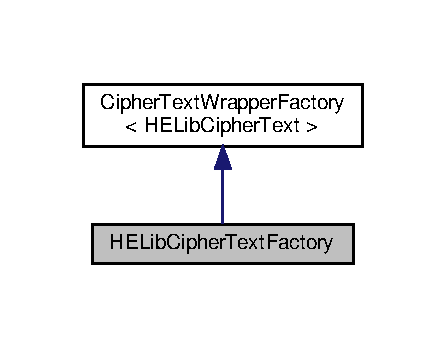
\includegraphics[width=214pt]{classHELibCipherTextFactory__inherit__graph}
\end{center}
\end{figure}


Collaboration diagram for H\+E\+Lib\+Cipher\+Text\+Factory\+:
\nopagebreak
\begin{figure}[H]
\begin{center}
\leavevmode
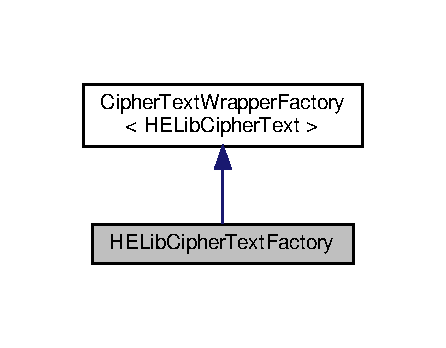
\includegraphics[width=214pt]{classHELibCipherTextFactory__coll__graph}
\end{center}
\end{figure}
\subsection*{Public Member Functions}
\begin{DoxyCompactItemize}
\item 
\hyperlink{classHELibCipherTextFactory_a097caa3314d257038989d27258cc9daf}{H\+E\+Lib\+Cipher\+Text\+Factory} (long seed=0, bool use\+B\+FV=true)
\item 
\hyperlink{classHELibCipherTextFactory_a725b27d7e0a60a6d2a9af33678f657be}{H\+E\+Lib\+Cipher\+Text\+Factory} (long L, long m, long r, long c=2)
\item 
\mbox{\Hypertarget{classHELibCipherTextFactory_aa262d2d08568dec07604be04f514bffd}\label{classHELibCipherTextFactory_aa262d2d08568dec07604be04f514bffd}} 
virtual \hyperlink{classHELibCipherText}{H\+E\+Lib\+Cipher\+Text} {\bfseries empty} () override
\item 
\mbox{\Hypertarget{classHELibCipherTextFactory_a438737fdf18c80a7552c15ad335217d4}\label{classHELibCipherTextFactory_a438737fdf18c80a7552c15ad335217d4}} 
virtual \hyperlink{classHELibCipherText}{H\+E\+Lib\+Cipher\+Text} {\bfseries create\+Cipher\+Text} (long x) override
\item 
\mbox{\Hypertarget{classHELibCipherTextFactory_a41b3d0604490f6135e0e729be22f28cb}\label{classHELibCipherTextFactory_a41b3d0604490f6135e0e729be22f28cb}} 
virtual \hyperlink{classHELibCipherText}{H\+E\+Lib\+Cipher\+Text} {\bfseries create\+Cipher\+Text} (const std\+::vector$<$ long $>$ \&in) override
\item 
\mbox{\Hypertarget{classHELibCipherTextFactory_af6fe83a8629c090430952229ec25b32c}\label{classHELibCipherTextFactory_af6fe83a8629c090430952229ec25b32c}} 
virtual \hyperlink{classHELibCipherText}{H\+E\+Lib\+Cipher\+Text} {\bfseries create\+Cipher\+Text} (const std\+::vector$<$ double $>$ \&in) override
\item 
\mbox{\Hypertarget{classHELibCipherTextFactory_afbd76ff874f2a66161ada236ca7652e4}\label{classHELibCipherTextFactory_afbd76ff874f2a66161ada236ca7652e4}} 
virtual \hyperlink{classHELibCipherText}{H\+E\+Lib\+Cipher\+Text} {\bfseries create\+Cipher\+Text} (const std\+::vector$<$ float $>$ \&in) override
\item 
\mbox{\Hypertarget{classHELibCipherTextFactory_a9f5ff1d324a4c4eab822ac2bbce2f12b}\label{classHELibCipherTextFactory_a9f5ff1d324a4c4eab822ac2bbce2f12b}} 
virtual std\+::vector$<$ long $>$ {\bfseries decrypt\+Long} (const \hyperlink{classHELibCipherText}{H\+E\+Lib\+Cipher\+Text} \&ctx) override
\item 
\mbox{\Hypertarget{classHELibCipherTextFactory_afce0ddd6b5d8215291b5a7d900010b1d}\label{classHELibCipherTextFactory_afce0ddd6b5d8215291b5a7d900010b1d}} 
virtual std\+::vector$<$ double $>$ {\bfseries decrypt\+Double} (const \hyperlink{classHELibCipherText}{H\+E\+Lib\+Cipher\+Text} \&ctx) override
\item 
\mbox{\Hypertarget{classHELibCipherTextFactory_a989b38ed86ad24c4c1da3d73b528af28}\label{classHELibCipherTextFactory_a989b38ed86ad24c4c1da3d73b528af28}} 
virtual void {\bfseries set\+As\+Default\+Factory} () override
\item 
\mbox{\Hypertarget{classHELibCipherTextFactory_a4cf13021fcce822cd1f0b5f08452cbbf}\label{classHELibCipherTextFactory_a4cf13021fcce822cd1f0b5f08452cbbf}} 
virtual TensorP$<$ \hyperlink{classHELibCipherText}{H\+E\+Lib\+Cipher\+Text} $>$ \hyperlink{classHELibCipherTextFactory_a4cf13021fcce822cd1f0b5f08452cbbf}{create\+Cipher\+Tensor} (const std\+::vector$<$ double $>$ \&in, const \hyperlink{classShape}{Shape} \&shape, \hyperlink{classHETensorFactory}{H\+E\+Tensor\+Factory}$<$ \hyperlink{classHELibCipherText}{H\+E\+Lib\+Cipher\+Text} $>$ $\ast$hetf) override
\begin{DoxyCompactList}\small\item\em Take a 1D vector transform into the given shape and encrypt it. The 1st dimension of the same needs to line up with the batch\+Size supported by the encryption scheme. \end{DoxyCompactList}\item 
\mbox{\Hypertarget{classHELibCipherTextFactory_a0c414fd65bc9d49c7a6ab349da26522d}\label{classHELibCipherTextFactory_a0c414fd65bc9d49c7a6ab349da26522d}} 
virtual TensorP$<$ \hyperlink{classHELibCipherText}{H\+E\+Lib\+Cipher\+Text} $>$ {\bfseries create\+Cipher\+Tensor} (const std\+::vector$<$ float $>$ \&in, const \hyperlink{classShape}{Shape} \&shape, \hyperlink{classHETensorFactory}{H\+E\+Tensor\+Factory}$<$ \hyperlink{classHELibCipherText}{H\+E\+Lib\+Cipher\+Text} $>$ $\ast$hetf) override
\item 
\mbox{\Hypertarget{classHELibCipherTextFactory_a9bdb6c404006f7876a7218a6fa48ba98}\label{classHELibCipherTextFactory_a9bdb6c404006f7876a7218a6fa48ba98}} 
virtual void {\bfseries feed\+Cipher\+Tensor} (const std\+::vector$<$ double $>$ \&in, TensorP$<$ \hyperlink{classHELibCipherText}{H\+E\+Lib\+Cipher\+Text} $>$ tensor) override
\item 
\mbox{\Hypertarget{classHELibCipherTextFactory_ae445259d96707e99490045ebb90b67d2}\label{classHELibCipherTextFactory_ae445259d96707e99490045ebb90b67d2}} 
virtual void {\bfseries feed\+Cipher\+Tensor} (const std\+::vector$<$ float $>$ \&in, TensorP$<$ \hyperlink{classHELibCipherText}{H\+E\+Lib\+Cipher\+Text} $>$ tensor) override
\item 
\mbox{\Hypertarget{classHELibCipherTextFactory_a4a2d8cbb37e7875a8b155f746852a244}\label{classHELibCipherTextFactory_a4a2d8cbb37e7875a8b155f746852a244}} 
virtual void {\bfseries feed\+Cipher\+Tensor} (const TensorP$<$ double $>$ in, TensorP$<$ \hyperlink{classHELibCipherText}{H\+E\+Lib\+Cipher\+Text} $>$ tensor) override
\item 
\mbox{\Hypertarget{classHELibCipherTextFactory_a609fb203aa9f501cc40394ba493c3d7c}\label{classHELibCipherTextFactory_a609fb203aa9f501cc40394ba493c3d7c}} 
virtual void {\bfseries feed\+Cipher\+Tensor} (const TensorP$<$ double $>$ in, \hyperlink{classTensor}{Tensor}$<$ \hyperlink{classHELibCipherText}{H\+E\+Lib\+Cipher\+Text} $>$ \&tensor) override
\item 
\mbox{\Hypertarget{classHELibCipherTextFactory_a0a1fe02c7af26a6fbcbfe2e6e1f362af}\label{classHELibCipherTextFactory_a0a1fe02c7af26a6fbcbfe2e6e1f362af}} 
virtual uint {\bfseries batchsize} () override
\item 
\mbox{\Hypertarget{classHELibCipherTextFactory_aa34268733c1b1497835d0014db8d13cd}\label{classHELibCipherTextFactory_aa34268733c1b1497835d0014db8d13cd}} 
std\+::shared\+\_\+ptr$<$ Ctxt $>$ {\bfseries create\+Raw\+Empty} ()
\end{DoxyCompactItemize}
\subsection*{Public Attributes}
\begin{DoxyCompactItemize}
\item 
\mbox{\Hypertarget{classHELibCipherTextFactory_a73742cada3eb2d6e1d6ac834de1b3ad0}\label{classHELibCipherTextFactory_a73742cada3eb2d6e1d6ac834de1b3ad0}} 
const bool {\bfseries use\+B\+FV}
\item 
\mbox{\Hypertarget{classHELibCipherTextFactory_aeb8b7ecb78a46467b70d0af21dbcc4ed}\label{classHELibCipherTextFactory_aeb8b7ecb78a46467b70d0af21dbcc4ed}} 
std\+::shared\+\_\+ptr$<$ F\+H\+E\+Sec\+Key $>$ {\bfseries secret\+Key}
\end{DoxyCompactItemize}


\subsection{Detailed Description}
Factory to create {\ttfamily \hyperlink{classHELibCipherText}{H\+E\+Lib\+Cipher\+Text}}

Supports both B\+FV and C\+K\+KS crypto schemes. B\+FV is not properly tested and might be removed in the future. The big drawback of B\+FV is that it does not supoort float numbers 

\subsection{Constructor \& Destructor Documentation}
\mbox{\Hypertarget{classHELibCipherTextFactory_a097caa3314d257038989d27258cc9daf}\label{classHELibCipherTextFactory_a097caa3314d257038989d27258cc9daf}} 
\index{H\+E\+Lib\+Cipher\+Text\+Factory@{H\+E\+Lib\+Cipher\+Text\+Factory}!H\+E\+Lib\+Cipher\+Text\+Factory@{H\+E\+Lib\+Cipher\+Text\+Factory}}
\index{H\+E\+Lib\+Cipher\+Text\+Factory@{H\+E\+Lib\+Cipher\+Text\+Factory}!H\+E\+Lib\+Cipher\+Text\+Factory@{H\+E\+Lib\+Cipher\+Text\+Factory}}
\subsubsection{\texorpdfstring{H\+E\+Lib\+Cipher\+Text\+Factory()}{HELibCipherTextFactory()}\hspace{0.1cm}{\footnotesize\ttfamily [1/2]}}
{\footnotesize\ttfamily H\+E\+Lib\+Cipher\+Text\+Factory\+::\+H\+E\+Lib\+Cipher\+Text\+Factory (\begin{DoxyParamCaption}\item[{long}]{seed = {\ttfamily 0},  }\item[{bool}]{use\+B\+FV = {\ttfamily true} }\end{DoxyParamCaption})\hspace{0.3cm}{\ttfamily [inline]}}

Number of levels in the modulus chain \mbox{[}default=heuristic\mbox{]} if used with out the FindM function it is Number of bits of the modulus chain

the ring we work on needs to a power of 2 Defines the batch\+Size. The batchsize is m/4

m specific the ring p = -\/1 means C\+K\+KS r is the number of bits after the decimal aka precision

just using the examples given by H\+E\+Lib docu. \mbox{\Hypertarget{classHELibCipherTextFactory_a725b27d7e0a60a6d2a9af33678f657be}\label{classHELibCipherTextFactory_a725b27d7e0a60a6d2a9af33678f657be}} 
\index{H\+E\+Lib\+Cipher\+Text\+Factory@{H\+E\+Lib\+Cipher\+Text\+Factory}!H\+E\+Lib\+Cipher\+Text\+Factory@{H\+E\+Lib\+Cipher\+Text\+Factory}}
\index{H\+E\+Lib\+Cipher\+Text\+Factory@{H\+E\+Lib\+Cipher\+Text\+Factory}!H\+E\+Lib\+Cipher\+Text\+Factory@{H\+E\+Lib\+Cipher\+Text\+Factory}}
\subsubsection{\texorpdfstring{H\+E\+Lib\+Cipher\+Text\+Factory()}{HELibCipherTextFactory()}\hspace{0.1cm}{\footnotesize\ttfamily [2/2]}}
{\footnotesize\ttfamily H\+E\+Lib\+Cipher\+Text\+Factory\+::\+H\+E\+Lib\+Cipher\+Text\+Factory (\begin{DoxyParamCaption}\item[{long}]{L,  }\item[{long}]{m,  }\item[{long}]{r,  }\item[{long}]{c = {\ttfamily 2} }\end{DoxyParamCaption})\hspace{0.3cm}{\ttfamily [inline]}}

m specific the ring p = -\/1 means C\+K\+KS r is the number of bits after the decimal aka precision

just using the examples given by H\+E\+Lib docu. 

The documentation for this class was generated from the following files\+:\begin{DoxyCompactItemize}
\item 
src/architecture/\+H\+E\+Backend/helib/H\+E\+L\+Ib\+Cipher\+Text.\+h\item 
src/architecture/\+H\+E\+Backend/helib/H\+E\+L\+Ib\+Cipher\+Text.\+cpp\end{DoxyCompactItemize}

\hypertarget{classHETensor}{}\section{H\+E\+Tensor$<$ T $>$ Class Template Reference}
\label{classHETensor}\index{H\+E\+Tensor$<$ T $>$@{H\+E\+Tensor$<$ T $>$}}


Inheritance diagram for H\+E\+Tensor$<$ T $>$\+:
\nopagebreak
\begin{figure}[H]
\begin{center}
\leavevmode
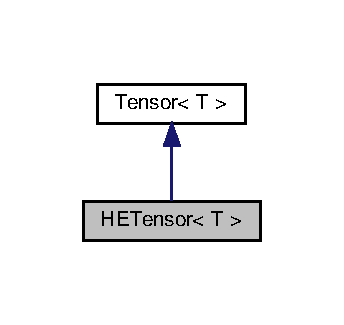
\includegraphics[width=165pt]{classHETensor__inherit__graph}
\end{center}
\end{figure}


Collaboration diagram for H\+E\+Tensor$<$ T $>$\+:
\nopagebreak
\begin{figure}[H]
\begin{center}
\leavevmode
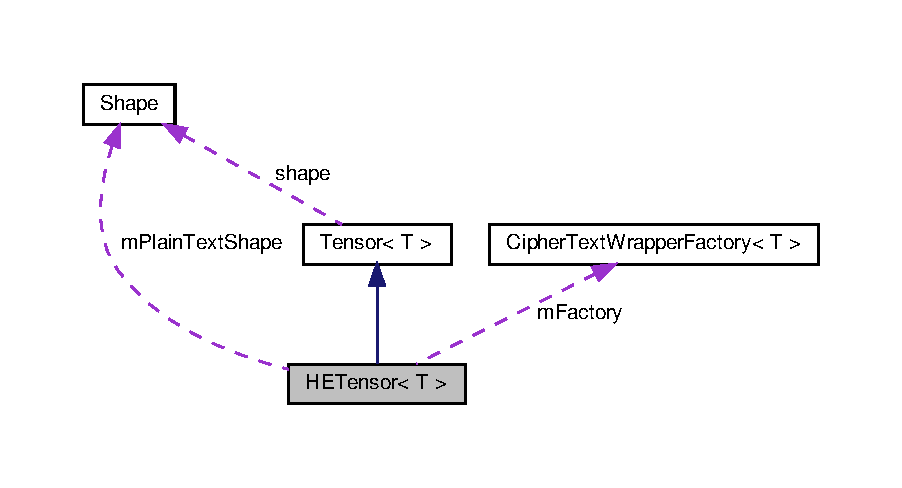
\includegraphics[width=350pt]{classHETensor__coll__graph}
\end{center}
\end{figure}
\subsection*{Public Member Functions}
\begin{DoxyCompactItemize}
\item 
\mbox{\Hypertarget{classHETensor_a7d20de8a5a4b73a5b26a530df8f5983f}\label{classHETensor_a7d20de8a5a4b73a5b26a530df8f5983f}} 
{\bfseries H\+E\+Tensor} (\hyperlink{classShape}{Shape} s, \hyperlink{classShape}{Shape} plain\+Text\+Shape, \hyperlink{classCipherTextWrapperFactory}{Cipher\+Text\+Wrapper\+Factory}$<$ T $>$ $\ast$factory)
\item 
\mbox{\Hypertarget{classHETensor_adfa6d2f93f822c6f7294728b59a400ee}\label{classHETensor_adfa6d2f93f822c6f7294728b59a400ee}} 
{\bfseries H\+E\+Tensor} (\hyperlink{classShape}{Shape} s, \hyperlink{classShape}{Shape} plain\+Text\+Shape, \hyperlink{classCipherTextWrapperFactory}{Cipher\+Text\+Wrapper\+Factory}$<$ T $>$ $\ast$factory, TensorP$<$ T $>$ other)
\item 
\mbox{\Hypertarget{classHETensor_a92788abf99e5d6773f021f1ef21886a7}\label{classHETensor_a92788abf99e5d6773f021f1ef21886a7}} 
virtual void \hyperlink{classHETensor_a92788abf99e5d6773f021f1ef21886a7}{perform\+Checks} () override
\begin{DoxyCompactList}\small\item\em Runs some checks on the content of the tensor. If the factory has {\ttfamily refresh\+On\+High\+Noise\+Enabled} this triggers the data to be sent to the client for rencryption. \end{DoxyCompactList}\item 
\mbox{\Hypertarget{classHETensor_af96ae9015195d89f91e44024cd6cc35c}\label{classHETensor_af96ae9015195d89f91e44024cd6cc35c}} 
TensorP$<$ double $>$ {\bfseries decrypt\+Double} ()
\item 
\mbox{\Hypertarget{classHETensor_aa52a0a3d339202b5dac7fcd507b00eb7}\label{classHETensor_aa52a0a3d339202b5dac7fcd507b00eb7}} 
TensorP$<$ long $>$ {\bfseries decrypt\+Long} ()
\item 
\mbox{\Hypertarget{classHETensor_a3f94bbe3c8bc5f29666cf309b9251abf}\label{classHETensor_a3f94bbe3c8bc5f29666cf309b9251abf}} 
virtual T {\bfseries empty} () override
\item 
\mbox{\Hypertarget{classHETensor_a0d9de653c9b2ec6963bb98ec5679be4b}\label{classHETensor_a0d9de653c9b2ec6963bb98ec5679be4b}} 
virtual std\+::vector$<$ int $>$ {\bfseries argmax\+Vector} (uint axis=0) override
\item 
\mbox{\Hypertarget{classHETensor_a9b58e05ba89b3c66084e33ca5423bbb6}\label{classHETensor_a9b58e05ba89b3c66084e33ca5423bbb6}} 
virtual void {\bfseries init} () override
\item 
\mbox{\Hypertarget{classHETensor_a171fd555451e5b9d6e71ebb871d368a3}\label{classHETensor_a171fd555451e5b9d6e71ebb871d368a3}} 
virtual void \hyperlink{classHETensor_a171fd555451e5b9d6e71ebb871d368a3}{init\+Random} (uint seed=7) override
\begin{DoxyCompactList}\small\item\em allocates the memory and fills it with random values \mbox{[}0,1\mbox{]} You can pass a seed for the random generator. Default seed is 7 \end{DoxyCompactList}\item 
\mbox{\Hypertarget{classHETensor_ac22b8062f261724d8a6a810d60a0d1cd}\label{classHETensor_ac22b8062f261724d8a6a810d60a0d1cd}} 
void \hyperlink{classHETensor_ac22b8062f261724d8a6a810d60a0d1cd}{refresh\+Cipher\+Texts} ()
\begin{DoxyCompactList}\small\item\em Refreshes the ciphertexts in the tensor. Currently they are decrypted and rencrypted. A more realistic implementation would send them to the holder of the private key. \end{DoxyCompactList}\end{DoxyCompactItemize}
\subsection*{Static Public Member Functions}
\begin{DoxyCompactItemize}
\item 
\mbox{\Hypertarget{classHETensor_a1b771ebed43f0ee13398a72837313ce4}\label{classHETensor_a1b771ebed43f0ee13398a72837313ce4}} 
static std\+::shared\+\_\+ptr$<$ \hyperlink{classHETensor}{H\+E\+Tensor}$<$ T $>$ $>$ {\bfseries create\+Tensor} (\hyperlink{classShape}{Shape} s, \hyperlink{classShape}{Shape} plain\+Text\+Shape, \hyperlink{classCipherTextWrapperFactory}{Cipher\+Text\+Wrapper\+Factory}$<$ T $>$ $\ast$factory)
\end{DoxyCompactItemize}
\subsection*{Protected Member Functions}
\begin{DoxyCompactItemize}
\item 
virtual void \hyperlink{classHETensor_ab0b9ca7b3826bc6c385514523e29de06}{compute\+Strides} () override
\item 
\mbox{\Hypertarget{classHETensor_a6c6723c9443c99e93b7135b6cd3d746e}\label{classHETensor_a6c6723c9443c99e93b7135b6cd3d746e}} 
virtual void {\bfseries create\+Storage} () override
\end{DoxyCompactItemize}
\subsection*{Protected Attributes}
\begin{DoxyCompactItemize}
\item 
\mbox{\Hypertarget{classHETensor_aa425107854263da0f5201441f28d06a4}\label{classHETensor_aa425107854263da0f5201441f28d06a4}} 
\hyperlink{classShape}{Shape} {\bfseries m\+Plain\+Text\+Shape}
\item 
\mbox{\Hypertarget{classHETensor_afba83053883bb84881f313074600af40}\label{classHETensor_afba83053883bb84881f313074600af40}} 
\hyperlink{classCipherTextWrapperFactory}{Cipher\+Text\+Wrapper\+Factory}$<$ T $>$ $\ast$ {\bfseries m\+Factory}
\end{DoxyCompactItemize}
\subsection*{Additional Inherited Members}


\subsection{Member Function Documentation}
\mbox{\Hypertarget{classHETensor_ab0b9ca7b3826bc6c385514523e29de06}\label{classHETensor_ab0b9ca7b3826bc6c385514523e29de06}} 
\index{H\+E\+Tensor@{H\+E\+Tensor}!compute\+Strides@{compute\+Strides}}
\index{compute\+Strides@{compute\+Strides}!H\+E\+Tensor@{H\+E\+Tensor}}
\subsubsection{\texorpdfstring{compute\+Strides()}{computeStrides()}}
{\footnotesize\ttfamily template$<$class T $>$ \\
virtual void \hyperlink{classHETensor}{H\+E\+Tensor}$<$ T $>$\+::compute\+Strides (\begin{DoxyParamCaption}{ }\end{DoxyParamCaption})\hspace{0.3cm}{\ttfamily [inline]}, {\ttfamily [override]}, {\ttfamily [protected]}, {\ttfamily [virtual]}}

Strides and shapes work somewhat differently with HE Tensors. Since we are working with S\+I\+MD our shape is \mbox{[} channel, y, x, batch \mbox{]}. This also changes the capacity of.

We want to keep the same shape notation as regular tensors. 

Reimplemented from \hyperlink{classTensor_a22b23dcd3dbe86924e01d13476f44204}{Tensor$<$ T $>$}.



The documentation for this class was generated from the following file\+:\begin{DoxyCompactItemize}
\item 
src/architecture/\+H\+E\+Backend/H\+E\+Tensor.\+h\end{DoxyCompactItemize}

\hypertarget{classHETensorFactory}{}\section{H\+E\+Tensor\+Factory$<$ T $>$ Class Template Reference}
\label{classHETensorFactory}\index{H\+E\+Tensor\+Factory$<$ T $>$@{H\+E\+Tensor\+Factory$<$ T $>$}}


Inheritance diagram for H\+E\+Tensor\+Factory$<$ T $>$\+:
\nopagebreak
\begin{figure}[H]
\begin{center}
\leavevmode
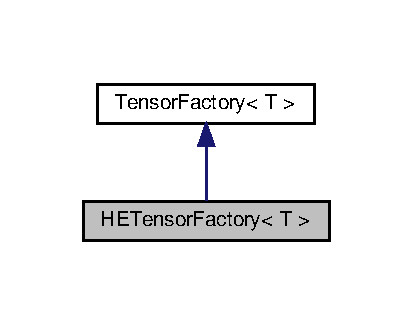
\includegraphics[width=198pt]{classHETensorFactory__inherit__graph}
\end{center}
\end{figure}


Collaboration diagram for H\+E\+Tensor\+Factory$<$ T $>$\+:
\nopagebreak
\begin{figure}[H]
\begin{center}
\leavevmode
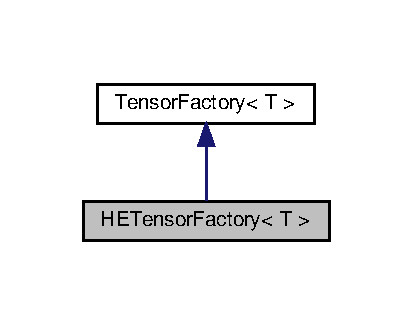
\includegraphics[width=198pt]{classHETensorFactory__coll__graph}
\end{center}
\end{figure}
\subsection*{Public Member Functions}
\begin{DoxyCompactItemize}
\item 
\mbox{\Hypertarget{classHETensorFactory_a5bc8ec357ccf999794e32e8e98ee8b01}\label{classHETensorFactory_a5bc8ec357ccf999794e32e8e98ee8b01}} 
{\bfseries H\+E\+Tensor\+Factory} (\hyperlink{classCipherTextWrapperFactory}{Cipher\+Text\+Wrapper\+Factory}$<$ T $>$ $\ast$factory)
\item 
virtual TensorP$<$ T $>$ \hyperlink{classHETensorFactory_a7becf968bdd7110f8f1ba7c2d212a69f}{create} (\hyperlink{classShape}{Shape} s) override
\item 
virtual TensorP$<$ T $>$ \hyperlink{classHETensorFactory_a9c8d6f82f1cbbdf497eb784b0c417f03}{create\+View} (\hyperlink{classShape}{Shape} s, TensorP$<$ T $>$ other) override
\begin{DoxyCompactList}\small\item\em Creates a different view on the same datastorage. Shapes must match. Views can alter the underlying data just as the original \hyperlink{classTensor}{Tensor}. After the creation they share equal ownership of the data. \end{DoxyCompactList}\item 
\mbox{\Hypertarget{classHETensorFactory_a73bfc12f4c1b6066da183e469dbb1d2c}\label{classHETensorFactory_a73bfc12f4c1b6066da183e469dbb1d2c}} 
\hyperlink{classCipherTextWrapperFactory}{Cipher\+Text\+Wrapper\+Factory}$<$ T $>$ $\ast$ {\bfseries ciphertext\+Factory} () const
\item 
\mbox{\Hypertarget{classHETensorFactory_abc9704a42a96acc8b195853c8c2e9a9a}\label{classHETensorFactory_abc9704a42a96acc8b195853c8c2e9a9a}} 
virtual TensorP$<$ T $>$ {\bfseries ones\+And\+Init} (\hyperlink{classShape}{Shape} s)
\item 
\mbox{\Hypertarget{classHETensorFactory_a7793cc289ab6ab739ed9e3b416dd4b22}\label{classHETensorFactory_a7793cc289ab6ab739ed9e3b416dd4b22}} 
virtual TensorP$<$ T $>$ {\bfseries arange\+And\+Init} (\hyperlink{classShape}{Shape} s, int start=1, int step=1)
\end{DoxyCompactItemize}


\subsection{Member Function Documentation}
\mbox{\Hypertarget{classHETensorFactory_a7becf968bdd7110f8f1ba7c2d212a69f}\label{classHETensorFactory_a7becf968bdd7110f8f1ba7c2d212a69f}} 
\index{H\+E\+Tensor\+Factory@{H\+E\+Tensor\+Factory}!create@{create}}
\index{create@{create}!H\+E\+Tensor\+Factory@{H\+E\+Tensor\+Factory}}
\subsubsection{\texorpdfstring{create()}{create()}}
{\footnotesize\ttfamily template$<$class T$>$ \\
virtual TensorP$<$T$>$ \hyperlink{classHETensorFactory}{H\+E\+Tensor\+Factory}$<$ T $>$\+::create (\begin{DoxyParamCaption}\item[{\hyperlink{classShape}{Shape}}]{s }\end{DoxyParamCaption})\hspace{0.3cm}{\ttfamily [inline]}, {\ttfamily [override]}, {\ttfamily [virtual]}}

Store the plain text shape for convience 

Implements \hyperlink{classTensorFactory}{Tensor\+Factory$<$ T $>$}.

\mbox{\Hypertarget{classHETensorFactory_a9c8d6f82f1cbbdf497eb784b0c417f03}\label{classHETensorFactory_a9c8d6f82f1cbbdf497eb784b0c417f03}} 
\index{H\+E\+Tensor\+Factory@{H\+E\+Tensor\+Factory}!create\+View@{create\+View}}
\index{create\+View@{create\+View}!H\+E\+Tensor\+Factory@{H\+E\+Tensor\+Factory}}
\subsubsection{\texorpdfstring{create\+View()}{createView()}}
{\footnotesize\ttfamily template$<$class T$>$ \\
virtual TensorP$<$T$>$ \hyperlink{classHETensorFactory}{H\+E\+Tensor\+Factory}$<$ T $>$\+::create\+View (\begin{DoxyParamCaption}\item[{\hyperlink{classShape}{Shape}}]{s,  }\item[{TensorP$<$ T $>$}]{other }\end{DoxyParamCaption})\hspace{0.3cm}{\ttfamily [inline]}, {\ttfamily [override]}, {\ttfamily [virtual]}}



Creates a different view on the same datastorage. Shapes must match. Views can alter the underlying data just as the original \hyperlink{classTensor}{Tensor}. After the creation they share equal ownership of the data. 

Store the plain text shape for convience 

Implements \hyperlink{classTensorFactory_ad14cbf4066594cc77f2fb75ee0a6ca74}{Tensor\+Factory$<$ T $>$}.



The documentation for this class was generated from the following files\+:\begin{DoxyCompactItemize}
\item 
src/architecture/\+H\+E\+Backend/Cipher\+Text\+Wrapper.\+h\item 
src/architecture/\+H\+E\+Backend/H\+E\+Tensor.\+h\end{DoxyCompactItemize}

\hypertarget{structnlohmann_1_1detail_1_1index__sequence}{}\section{nlohmann\+:\+:detail\+:\+:index\+\_\+sequence$<$ Ints $>$ Struct Template Reference}
\label{structnlohmann_1_1detail_1_1index__sequence}\index{nlohmann\+::detail\+::index\+\_\+sequence$<$ Ints $>$@{nlohmann\+::detail\+::index\+\_\+sequence$<$ Ints $>$}}
\subsection*{Public Types}
\begin{DoxyCompactItemize}
\item 
\mbox{\Hypertarget{structnlohmann_1_1detail_1_1index__sequence_a3c14c4ab277de72b166806193ff4fa10}\label{structnlohmann_1_1detail_1_1index__sequence_a3c14c4ab277de72b166806193ff4fa10}} 
using {\bfseries type} = \hyperlink{structnlohmann_1_1detail_1_1index__sequence}{index\+\_\+sequence}
\item 
\mbox{\Hypertarget{structnlohmann_1_1detail_1_1index__sequence_a2eca43d08fc1eb68bd5fa75b6714d21d}\label{structnlohmann_1_1detail_1_1index__sequence_a2eca43d08fc1eb68bd5fa75b6714d21d}} 
using {\bfseries value\+\_\+type} = std\+::size\+\_\+t
\end{DoxyCompactItemize}
\subsection*{Static Public Member Functions}
\begin{DoxyCompactItemize}
\item 
\mbox{\Hypertarget{structnlohmann_1_1detail_1_1index__sequence_a7ac529419787d775f52408135304b337}\label{structnlohmann_1_1detail_1_1index__sequence_a7ac529419787d775f52408135304b337}} 
static constexpr std\+::size\+\_\+t {\bfseries size} () noexcept
\end{DoxyCompactItemize}


The documentation for this struct was generated from the following file\+:\begin{DoxyCompactItemize}
\item 
src/tools/json/json.\+hpp\end{DoxyCompactItemize}

\hypertarget{classnlohmann_1_1detail_1_1input__adapter}{}\section{nlohmann\+:\+:detail\+:\+:input\+\_\+adapter Class Reference}
\label{classnlohmann_1_1detail_1_1input__adapter}\index{nlohmann\+::detail\+::input\+\_\+adapter@{nlohmann\+::detail\+::input\+\_\+adapter}}
\subsection*{Public Member Functions}
\begin{DoxyCompactItemize}
\item 
\mbox{\Hypertarget{classnlohmann_1_1detail_1_1input__adapter_a19fb8c28f37b23099a4353acf0a9a2f1}\label{classnlohmann_1_1detail_1_1input__adapter_a19fb8c28f37b23099a4353acf0a9a2f1}} 
{\bfseries input\+\_\+adapter} (std\+::\+F\+I\+LE $\ast$file)
\item 
\mbox{\Hypertarget{classnlohmann_1_1detail_1_1input__adapter_ae89f11268d4724b3080473f7218abe86}\label{classnlohmann_1_1detail_1_1input__adapter_ae89f11268d4724b3080473f7218abe86}} 
\hyperlink{classnlohmann_1_1detail_1_1input__adapter_ae89f11268d4724b3080473f7218abe86}{input\+\_\+adapter} (std\+::istream \&i)
\begin{DoxyCompactList}\small\item\em input adapter for input stream \end{DoxyCompactList}\item 
\mbox{\Hypertarget{classnlohmann_1_1detail_1_1input__adapter_af002dd2e53ac0855a03cb68d0ce626b2}\label{classnlohmann_1_1detail_1_1input__adapter_af002dd2e53ac0855a03cb68d0ce626b2}} 
\hyperlink{classnlohmann_1_1detail_1_1input__adapter_af002dd2e53ac0855a03cb68d0ce626b2}{input\+\_\+adapter} (std\+::istream \&\&i)
\begin{DoxyCompactList}\small\item\em input adapter for input stream \end{DoxyCompactList}\item 
\mbox{\Hypertarget{classnlohmann_1_1detail_1_1input__adapter_a32f5ddd06562edce43ee86f5b5c2031b}\label{classnlohmann_1_1detail_1_1input__adapter_a32f5ddd06562edce43ee86f5b5c2031b}} 
{\bfseries input\+\_\+adapter} (const std\+::wstring \&ws)
\item 
\mbox{\Hypertarget{classnlohmann_1_1detail_1_1input__adapter_a58163eaa485b17dd878d3c782efc1e43}\label{classnlohmann_1_1detail_1_1input__adapter_a58163eaa485b17dd878d3c782efc1e43}} 
{\bfseries input\+\_\+adapter} (const std\+::u16string \&ws)
\item 
\mbox{\Hypertarget{classnlohmann_1_1detail_1_1input__adapter_abe0015ae09e855f502620315b9dcc3db}\label{classnlohmann_1_1detail_1_1input__adapter_abe0015ae09e855f502620315b9dcc3db}} 
{\bfseries input\+\_\+adapter} (const std\+::u32string \&ws)
\item 
\mbox{\Hypertarget{classnlohmann_1_1detail_1_1input__adapter_a37816622d79ab4a1a76f4d7e872b65e1}\label{classnlohmann_1_1detail_1_1input__adapter_a37816622d79ab4a1a76f4d7e872b65e1}} 
{\footnotesize template$<$typename CharT , typename std\+::enable\+\_\+if$<$ std\+::is\+\_\+pointer$<$ Char\+T $>$\+::value and std\+::is\+\_\+integral$<$ typename std\+::remove\+\_\+pointer$<$ Char\+T $>$\+::type $>$\+::value and sizeof(typename std\+::remove\+\_\+pointer$<$ Char\+T $>$\+::type)==1, int $>$\+::type  = 0$>$ }\\\hyperlink{classnlohmann_1_1detail_1_1input__adapter_a37816622d79ab4a1a76f4d7e872b65e1}{input\+\_\+adapter} (CharT b, std\+::size\+\_\+t l)
\begin{DoxyCompactList}\small\item\em input adapter for buffer \end{DoxyCompactList}\item 
\mbox{\Hypertarget{classnlohmann_1_1detail_1_1input__adapter_a86f035d9c4319360014b922b5e433ced}\label{classnlohmann_1_1detail_1_1input__adapter_a86f035d9c4319360014b922b5e433ced}} 
{\footnotesize template$<$typename CharT , typename std\+::enable\+\_\+if$<$ std\+::is\+\_\+pointer$<$ Char\+T $>$\+::value and std\+::is\+\_\+integral$<$ typename std\+::remove\+\_\+pointer$<$ Char\+T $>$\+::type $>$\+::value and sizeof(typename std\+::remove\+\_\+pointer$<$ Char\+T $>$\+::type)==1, int $>$\+::type  = 0$>$ }\\\hyperlink{classnlohmann_1_1detail_1_1input__adapter_a86f035d9c4319360014b922b5e433ced}{input\+\_\+adapter} (CharT b)
\begin{DoxyCompactList}\small\item\em input adapter for string literal \end{DoxyCompactList}\item 
\mbox{\Hypertarget{classnlohmann_1_1detail_1_1input__adapter_ad6824b0f792691f75186c527fa31a6b4}\label{classnlohmann_1_1detail_1_1input__adapter_ad6824b0f792691f75186c527fa31a6b4}} 
{\footnotesize template$<$class Iterator\+Type , typename std\+::enable\+\_\+if$<$ std\+::is\+\_\+same$<$ typename iterator\+\_\+traits$<$ Iterator\+Type $>$\+::iterator\+\_\+category, std\+::random\+\_\+access\+\_\+iterator\+\_\+tag $>$\+::value, int $>$\+::type  = 0$>$ }\\\hyperlink{classnlohmann_1_1detail_1_1input__adapter_ad6824b0f792691f75186c527fa31a6b4}{input\+\_\+adapter} (Iterator\+Type first, Iterator\+Type last)
\begin{DoxyCompactList}\small\item\em input adapter for iterator range with contiguous storage \end{DoxyCompactList}\item 
\mbox{\Hypertarget{classnlohmann_1_1detail_1_1input__adapter_aa2392138bf8307df1994dc7eb22d51ce}\label{classnlohmann_1_1detail_1_1input__adapter_aa2392138bf8307df1994dc7eb22d51ce}} 
{\footnotesize template$<$class T , std\+::size\+\_\+t N$>$ }\\\hyperlink{classnlohmann_1_1detail_1_1input__adapter_aa2392138bf8307df1994dc7eb22d51ce}{input\+\_\+adapter} (T(\&\hyperlink{namespacenlohmann_1_1detail_a1ed8fc6239da25abcaf681d30ace4985af1f713c9e000f5d3f280adbd124df4f5}{array})\mbox{[}N\mbox{]})
\begin{DoxyCompactList}\small\item\em input adapter for array \end{DoxyCompactList}\item 
\mbox{\Hypertarget{classnlohmann_1_1detail_1_1input__adapter_a6f92fe82cb49a508dbfb297c5630cc7f}\label{classnlohmann_1_1detail_1_1input__adapter_a6f92fe82cb49a508dbfb297c5630cc7f}} 
{\footnotesize template$<$class Contiguous\+Container , typename std\+::enable\+\_\+if$<$ not std\+::is\+\_\+pointer$<$ Contiguous\+Container $>$\+::value and std\+::is\+\_\+base\+\_\+of$<$ std\+::random\+\_\+access\+\_\+iterator\+\_\+tag, typename iterator\+\_\+traits$<$ decltype(std\+::begin(std\+::declval$<$ Contiguous\+Container const $>$()))$>$\+::iterator\+\_\+category $>$\+::value, int $>$\+::type  = 0$>$ }\\\hyperlink{classnlohmann_1_1detail_1_1input__adapter_a6f92fe82cb49a508dbfb297c5630cc7f}{input\+\_\+adapter} (const Contiguous\+Container \&c)
\begin{DoxyCompactList}\small\item\em input adapter for contiguous container \end{DoxyCompactList}\item 
\mbox{\Hypertarget{classnlohmann_1_1detail_1_1input__adapter_a4ef04b9490247fc38f3d1c2a9e18789b}\label{classnlohmann_1_1detail_1_1input__adapter_a4ef04b9490247fc38f3d1c2a9e18789b}} 
{\bfseries operator input\+\_\+adapter\+\_\+t} ()
\end{DoxyCompactItemize}


The documentation for this class was generated from the following file\+:\begin{DoxyCompactItemize}
\item 
src/tools/json/json.\+hpp\end{DoxyCompactItemize}

\hypertarget{structnlohmann_1_1detail_1_1input__adapter__protocol}{}\section{nlohmann\+:\+:detail\+:\+:input\+\_\+adapter\+\_\+protocol Struct Reference}
\label{structnlohmann_1_1detail_1_1input__adapter__protocol}\index{nlohmann\+::detail\+::input\+\_\+adapter\+\_\+protocol@{nlohmann\+::detail\+::input\+\_\+adapter\+\_\+protocol}}


abstract input adapter interface  




{\ttfamily \#include $<$json.\+hpp$>$}



Inheritance diagram for nlohmann\+:\+:detail\+:\+:input\+\_\+adapter\+\_\+protocol\+:
\nopagebreak
\begin{figure}[H]
\begin{center}
\leavevmode
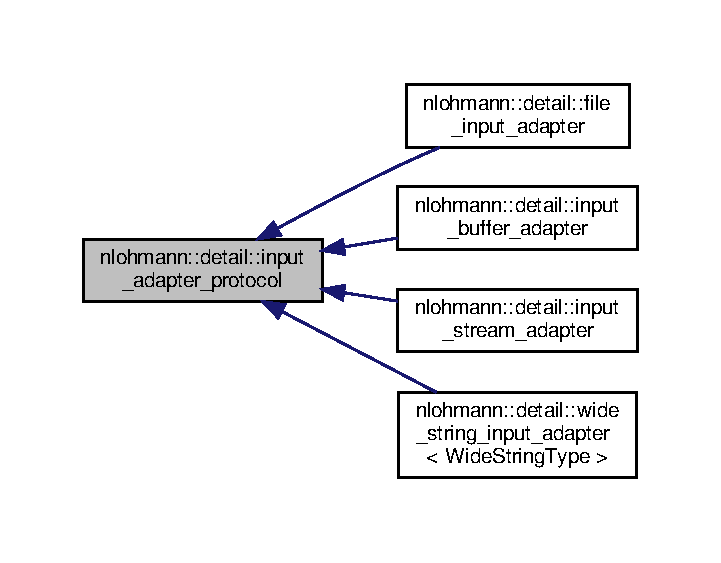
\includegraphics[width=346pt]{structnlohmann_1_1detail_1_1input__adapter__protocol__inherit__graph}
\end{center}
\end{figure}
\subsection*{Public Member Functions}
\begin{DoxyCompactItemize}
\item 
\mbox{\Hypertarget{structnlohmann_1_1detail_1_1input__adapter__protocol_aac10a6a4048a8ce8e2ed50277692a3ca}\label{structnlohmann_1_1detail_1_1input__adapter__protocol_aac10a6a4048a8ce8e2ed50277692a3ca}} 
virtual std\+::char\+\_\+traits$<$ char $>$\+::int\+\_\+type \hyperlink{structnlohmann_1_1detail_1_1input__adapter__protocol_aac10a6a4048a8ce8e2ed50277692a3ca}{get\+\_\+character} ()=0
\begin{DoxyCompactList}\small\item\em get a character \mbox{[}0,255\mbox{]} or std\+::char\+\_\+traits$<$char$>$\+::eof(). \end{DoxyCompactList}\end{DoxyCompactItemize}


\subsection{Detailed Description}
abstract input adapter interface 

Produces a stream of std\+::char\+\_\+traits$<$char$>$\+::int\+\_\+type characters from a std\+::istream, a buffer, or some other input type. Accepts the return of exactly one non-\/\+E\+OF character for future input. The int\+\_\+type characters returned consist of all valid char values as positive values (typically unsigned char), plus an E\+OF value outside that range, specified by the value of the function std\+::char\+\_\+traits$<$char$>$\+::eof(). This value is typically -\/1, but could be any arbitrary value which is not a valid char value. 

The documentation for this struct was generated from the following file\+:\begin{DoxyCompactItemize}
\item 
src/tools/json/json.\+hpp\end{DoxyCompactItemize}

\hypertarget{classnlohmann_1_1detail_1_1input__buffer__adapter}{}\section{nlohmann\+:\+:detail\+:\+:input\+\_\+buffer\+\_\+adapter Class Reference}
\label{classnlohmann_1_1detail_1_1input__buffer__adapter}\index{nlohmann\+::detail\+::input\+\_\+buffer\+\_\+adapter@{nlohmann\+::detail\+::input\+\_\+buffer\+\_\+adapter}}


input adapter for buffer input  




{\ttfamily \#include $<$json.\+hpp$>$}



Inheritance diagram for nlohmann\+:\+:detail\+:\+:input\+\_\+buffer\+\_\+adapter\+:
\nopagebreak
\begin{figure}[H]
\begin{center}
\leavevmode
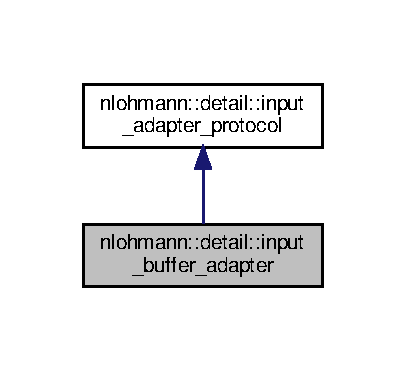
\includegraphics[width=195pt]{classnlohmann_1_1detail_1_1input__buffer__adapter__inherit__graph}
\end{center}
\end{figure}


Collaboration diagram for nlohmann\+:\+:detail\+:\+:input\+\_\+buffer\+\_\+adapter\+:
\nopagebreak
\begin{figure}[H]
\begin{center}
\leavevmode
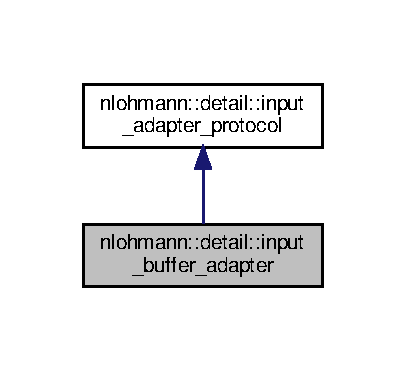
\includegraphics[width=195pt]{classnlohmann_1_1detail_1_1input__buffer__adapter__coll__graph}
\end{center}
\end{figure}
\subsection*{Public Member Functions}
\begin{DoxyCompactItemize}
\item 
\mbox{\Hypertarget{classnlohmann_1_1detail_1_1input__buffer__adapter_ad9b912fabdcb53de255e8c444d625ac3}\label{classnlohmann_1_1detail_1_1input__buffer__adapter_ad9b912fabdcb53de255e8c444d625ac3}} 
{\bfseries input\+\_\+buffer\+\_\+adapter} (const char $\ast$b, const std\+::size\+\_\+t l) noexcept
\item 
\mbox{\Hypertarget{classnlohmann_1_1detail_1_1input__buffer__adapter_ada76d7b75c5d6b989af0e18687ef07b6}\label{classnlohmann_1_1detail_1_1input__buffer__adapter_ada76d7b75c5d6b989af0e18687ef07b6}} 
{\bfseries input\+\_\+buffer\+\_\+adapter} (const \hyperlink{classnlohmann_1_1detail_1_1input__buffer__adapter}{input\+\_\+buffer\+\_\+adapter} \&)=delete
\item 
\mbox{\Hypertarget{classnlohmann_1_1detail_1_1input__buffer__adapter_a0871125057d993684ba8e45fb2b8a76b}\label{classnlohmann_1_1detail_1_1input__buffer__adapter_a0871125057d993684ba8e45fb2b8a76b}} 
\hyperlink{classnlohmann_1_1detail_1_1input__buffer__adapter}{input\+\_\+buffer\+\_\+adapter} \& {\bfseries operator=} (\hyperlink{classnlohmann_1_1detail_1_1input__buffer__adapter}{input\+\_\+buffer\+\_\+adapter} \&)=delete
\item 
\mbox{\Hypertarget{classnlohmann_1_1detail_1_1input__buffer__adapter_ab6bc6bb785408b74af284a5b7544d9dc}\label{classnlohmann_1_1detail_1_1input__buffer__adapter_ab6bc6bb785408b74af284a5b7544d9dc}} 
{\bfseries input\+\_\+buffer\+\_\+adapter} (\hyperlink{classnlohmann_1_1detail_1_1input__buffer__adapter}{input\+\_\+buffer\+\_\+adapter} \&\&)=delete
\item 
\mbox{\Hypertarget{classnlohmann_1_1detail_1_1input__buffer__adapter_a19bb3ff68048a2fc8ecc41a013af37ae}\label{classnlohmann_1_1detail_1_1input__buffer__adapter_a19bb3ff68048a2fc8ecc41a013af37ae}} 
\hyperlink{classnlohmann_1_1detail_1_1input__buffer__adapter}{input\+\_\+buffer\+\_\+adapter} \& {\bfseries operator=} (\hyperlink{classnlohmann_1_1detail_1_1input__buffer__adapter}{input\+\_\+buffer\+\_\+adapter} \&\&)=delete
\item 
\mbox{\Hypertarget{classnlohmann_1_1detail_1_1input__buffer__adapter_ae9e195b04f3551fafb0925aafba00124}\label{classnlohmann_1_1detail_1_1input__buffer__adapter_ae9e195b04f3551fafb0925aafba00124}} 
std\+::char\+\_\+traits$<$ char $>$\+::int\+\_\+type \hyperlink{classnlohmann_1_1detail_1_1input__buffer__adapter_ae9e195b04f3551fafb0925aafba00124}{get\+\_\+character} () noexcept override
\begin{DoxyCompactList}\small\item\em get a character \mbox{[}0,255\mbox{]} or std\+::char\+\_\+traits$<$char$>$\+::eof(). \end{DoxyCompactList}\end{DoxyCompactItemize}


\subsection{Detailed Description}
input adapter for buffer input 

The documentation for this class was generated from the following file\+:\begin{DoxyCompactItemize}
\item 
src/tools/json/json.\+hpp\end{DoxyCompactItemize}

\hypertarget{classnlohmann_1_1detail_1_1input__stream__adapter}{}\section{nlohmann\+:\+:detail\+:\+:input\+\_\+stream\+\_\+adapter Class Reference}
\label{classnlohmann_1_1detail_1_1input__stream__adapter}\index{nlohmann\+::detail\+::input\+\_\+stream\+\_\+adapter@{nlohmann\+::detail\+::input\+\_\+stream\+\_\+adapter}}


{\ttfamily \#include $<$json.\+hpp$>$}



Inheritance diagram for nlohmann\+:\+:detail\+:\+:input\+\_\+stream\+\_\+adapter\+:
\nopagebreak
\begin{figure}[H]
\begin{center}
\leavevmode
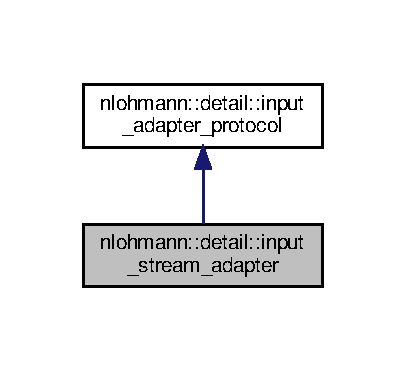
\includegraphics[width=195pt]{classnlohmann_1_1detail_1_1input__stream__adapter__inherit__graph}
\end{center}
\end{figure}


Collaboration diagram for nlohmann\+:\+:detail\+:\+:input\+\_\+stream\+\_\+adapter\+:
\nopagebreak
\begin{figure}[H]
\begin{center}
\leavevmode
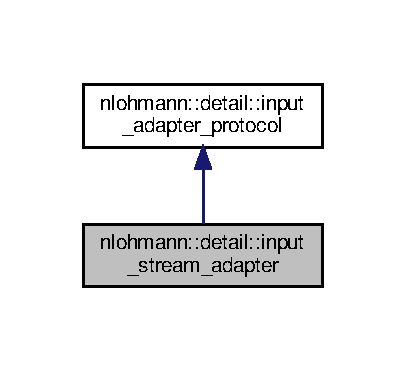
\includegraphics[width=195pt]{classnlohmann_1_1detail_1_1input__stream__adapter__coll__graph}
\end{center}
\end{figure}
\subsection*{Public Member Functions}
\begin{DoxyCompactItemize}
\item 
\mbox{\Hypertarget{classnlohmann_1_1detail_1_1input__stream__adapter_af487152e4606d013eb4ec6a90eaf82ea}\label{classnlohmann_1_1detail_1_1input__stream__adapter_af487152e4606d013eb4ec6a90eaf82ea}} 
{\bfseries input\+\_\+stream\+\_\+adapter} (std\+::istream \&i)
\item 
\mbox{\Hypertarget{classnlohmann_1_1detail_1_1input__stream__adapter_a5190fe4d0c5ff2e3b348b28ee3bb2218}\label{classnlohmann_1_1detail_1_1input__stream__adapter_a5190fe4d0c5ff2e3b348b28ee3bb2218}} 
{\bfseries input\+\_\+stream\+\_\+adapter} (const \hyperlink{classnlohmann_1_1detail_1_1input__stream__adapter}{input\+\_\+stream\+\_\+adapter} \&)=delete
\item 
\mbox{\Hypertarget{classnlohmann_1_1detail_1_1input__stream__adapter_aeac5048221929b8f7558d1698dd0fb3a}\label{classnlohmann_1_1detail_1_1input__stream__adapter_aeac5048221929b8f7558d1698dd0fb3a}} 
\hyperlink{classnlohmann_1_1detail_1_1input__stream__adapter}{input\+\_\+stream\+\_\+adapter} \& {\bfseries operator=} (\hyperlink{classnlohmann_1_1detail_1_1input__stream__adapter}{input\+\_\+stream\+\_\+adapter} \&)=delete
\item 
\mbox{\Hypertarget{classnlohmann_1_1detail_1_1input__stream__adapter_a0ae74b874f7db43640905cb7f2442b1d}\label{classnlohmann_1_1detail_1_1input__stream__adapter_a0ae74b874f7db43640905cb7f2442b1d}} 
{\bfseries input\+\_\+stream\+\_\+adapter} (\hyperlink{classnlohmann_1_1detail_1_1input__stream__adapter}{input\+\_\+stream\+\_\+adapter} \&\&)=delete
\item 
\mbox{\Hypertarget{classnlohmann_1_1detail_1_1input__stream__adapter_a3577dff99cc91968557b52959b0363e4}\label{classnlohmann_1_1detail_1_1input__stream__adapter_a3577dff99cc91968557b52959b0363e4}} 
\hyperlink{classnlohmann_1_1detail_1_1input__stream__adapter}{input\+\_\+stream\+\_\+adapter} \& {\bfseries operator=} (\hyperlink{classnlohmann_1_1detail_1_1input__stream__adapter}{input\+\_\+stream\+\_\+adapter} \&\&)=delete
\item 
\mbox{\Hypertarget{classnlohmann_1_1detail_1_1input__stream__adapter_ae0760af923583de6354725e901d1869d}\label{classnlohmann_1_1detail_1_1input__stream__adapter_ae0760af923583de6354725e901d1869d}} 
std\+::char\+\_\+traits$<$ char $>$\+::int\+\_\+type \hyperlink{classnlohmann_1_1detail_1_1input__stream__adapter_ae0760af923583de6354725e901d1869d}{get\+\_\+character} () override
\begin{DoxyCompactList}\small\item\em get a character \mbox{[}0,255\mbox{]} or std\+::char\+\_\+traits$<$char$>$\+::eof(). \end{DoxyCompactList}\end{DoxyCompactItemize}


\subsection{Detailed Description}
Input adapter for a (caching) istream. Ignores a U\+FT Byte Order Mark at beginning of input. Does not support changing the underlying std\+::streambuf in mid-\/input. Maintains underlying std\+::istream and std\+::streambuf to support subsequent use of standard std\+::istream operations to process any input characters following those used in parsing the J\+S\+ON input. Clears the std\+::istream flags; any input errors (e.\+g., E\+OF) will be detected by the first subsequent call for input from the std\+::istream. 

The documentation for this class was generated from the following file\+:\begin{DoxyCompactItemize}
\item 
src/tools/json/json.\+hpp\end{DoxyCompactItemize}

\hypertarget{structnlohmann_1_1detail_1_1internal__iterator}{}\section{nlohmann\+:\+:detail\+:\+:internal\+\_\+iterator$<$ Basic\+Json\+Type $>$ Struct Template Reference}
\label{structnlohmann_1_1detail_1_1internal__iterator}\index{nlohmann\+::detail\+::internal\+\_\+iterator$<$ Basic\+Json\+Type $>$@{nlohmann\+::detail\+::internal\+\_\+iterator$<$ Basic\+Json\+Type $>$}}


an iterator value  




{\ttfamily \#include $<$json.\+hpp$>$}



Collaboration diagram for nlohmann\+:\+:detail\+:\+:internal\+\_\+iterator$<$ Basic\+Json\+Type $>$\+:
\nopagebreak
\begin{figure}[H]
\begin{center}
\leavevmode
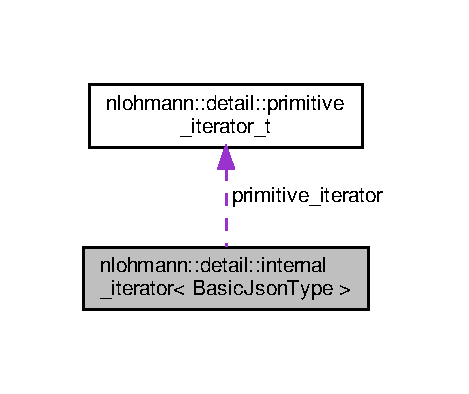
\includegraphics[width=225pt]{structnlohmann_1_1detail_1_1internal__iterator__coll__graph}
\end{center}
\end{figure}
\subsection*{Public Attributes}
\begin{DoxyCompactItemize}
\item 
\mbox{\Hypertarget{structnlohmann_1_1detail_1_1internal__iterator_a8cb0af3498061426c1d0a65ad6220408}\label{structnlohmann_1_1detail_1_1internal__iterator_a8cb0af3498061426c1d0a65ad6220408}} 
Basic\+Json\+Type\+::object\+\_\+t\+::iterator \hyperlink{structnlohmann_1_1detail_1_1internal__iterator_a8cb0af3498061426c1d0a65ad6220408}{object\+\_\+iterator} \{\}
\begin{DoxyCompactList}\small\item\em iterator for J\+S\+ON objects \end{DoxyCompactList}\item 
\mbox{\Hypertarget{structnlohmann_1_1detail_1_1internal__iterator_a8294a6e6f01b58e1cce8fbae66a50b5d}\label{structnlohmann_1_1detail_1_1internal__iterator_a8294a6e6f01b58e1cce8fbae66a50b5d}} 
Basic\+Json\+Type\+::array\+\_\+t\+::iterator \hyperlink{structnlohmann_1_1detail_1_1internal__iterator_a8294a6e6f01b58e1cce8fbae66a50b5d}{array\+\_\+iterator} \{\}
\begin{DoxyCompactList}\small\item\em iterator for J\+S\+ON arrays \end{DoxyCompactList}\item 
\mbox{\Hypertarget{structnlohmann_1_1detail_1_1internal__iterator_a2b3bb45f968210e42c282017eeeb63a8}\label{structnlohmann_1_1detail_1_1internal__iterator_a2b3bb45f968210e42c282017eeeb63a8}} 
\hyperlink{classnlohmann_1_1detail_1_1primitive__iterator__t}{primitive\+\_\+iterator\+\_\+t} \hyperlink{structnlohmann_1_1detail_1_1internal__iterator_a2b3bb45f968210e42c282017eeeb63a8}{primitive\+\_\+iterator} \{\}
\begin{DoxyCompactList}\small\item\em generic iterator for all other types \end{DoxyCompactList}\end{DoxyCompactItemize}


\subsection{Detailed Description}
\subsubsection*{template$<$typename Basic\+Json\+Type$>$\newline
struct nlohmann\+::detail\+::internal\+\_\+iterator$<$ Basic\+Json\+Type $>$}

an iterator value 

\begin{DoxyNote}{Note}
This structure could easily be a union, but M\+S\+VC currently does not allow unions members with complex constructors, see \href{https://github.com/nlohmann/json/pull/105}{\tt https\+://github.\+com/nlohmann/json/pull/105}. 
\end{DoxyNote}


The documentation for this struct was generated from the following file\+:\begin{DoxyCompactItemize}
\item 
src/tools/json/json.\+hpp\end{DoxyCompactItemize}

\hypertarget{classnlohmann_1_1detail_1_1invalid__iterator}{}\section{nlohmann\+:\+:detail\+:\+:invalid\+\_\+iterator Class Reference}
\label{classnlohmann_1_1detail_1_1invalid__iterator}\index{nlohmann\+::detail\+::invalid\+\_\+iterator@{nlohmann\+::detail\+::invalid\+\_\+iterator}}


exception indicating errors with iterators  




{\ttfamily \#include $<$json.\+hpp$>$}



Inheritance diagram for nlohmann\+:\+:detail\+:\+:invalid\+\_\+iterator\+:
\nopagebreak
\begin{figure}[H]
\begin{center}
\leavevmode
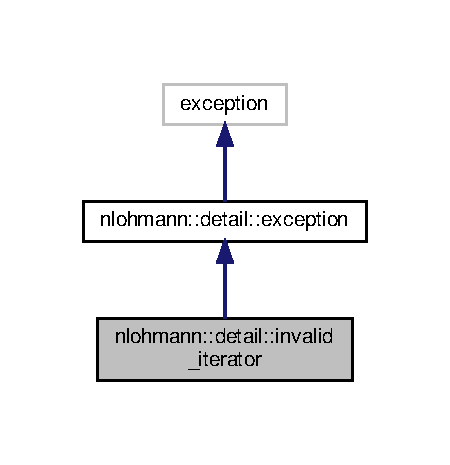
\includegraphics[width=216pt]{classnlohmann_1_1detail_1_1invalid__iterator__inherit__graph}
\end{center}
\end{figure}


Collaboration diagram for nlohmann\+:\+:detail\+:\+:invalid\+\_\+iterator\+:
\nopagebreak
\begin{figure}[H]
\begin{center}
\leavevmode
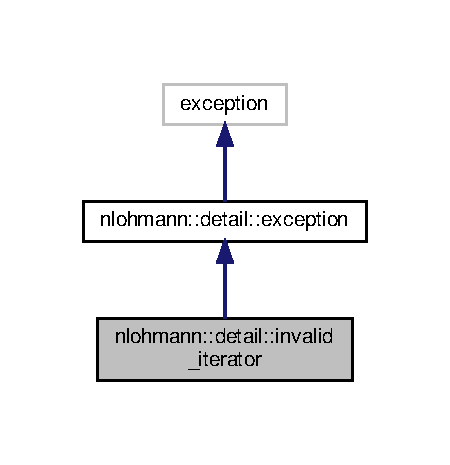
\includegraphics[width=216pt]{classnlohmann_1_1detail_1_1invalid__iterator__coll__graph}
\end{center}
\end{figure}
\subsection*{Static Public Member Functions}
\begin{DoxyCompactItemize}
\item 
\mbox{\Hypertarget{classnlohmann_1_1detail_1_1invalid__iterator_a4e849260a3caa1b288c7e619130c6c09}\label{classnlohmann_1_1detail_1_1invalid__iterator_a4e849260a3caa1b288c7e619130c6c09}} 
static \hyperlink{classnlohmann_1_1detail_1_1invalid__iterator}{invalid\+\_\+iterator} {\bfseries create} (int id\+\_\+, const \hyperlink{namespacenlohmann_1_1detail_a1ed8fc6239da25abcaf681d30ace4985ab45cffe084dd3d20d928bee85e7b0f21}{std\+::string} \&what\+\_\+arg)
\end{DoxyCompactItemize}
\subsection*{Additional Inherited Members}


\subsection{Detailed Description}
exception indicating errors with iterators 

This exception is thrown if iterators passed to a library function do not match the expected semantics.

Exceptions have ids 2xx.

\tabulinesep=1mm
\begin{longtabu} spread 0pt [c]{*{3}{|X[-1]}|}
\hline
\rowcolor{\tableheadbgcolor}\textbf{ name / id }&\textbf{ example message }&\textbf{ description  }\\\cline{1-3}
\endfirsthead
\hline
\endfoot
\hline
\rowcolor{\tableheadbgcolor}\textbf{ name / id }&\textbf{ example message }&\textbf{ description  }\\\cline{1-3}
\endhead
json.\+exception.\+invalid\+\_\+iterator.\+201 &iterators are not compatible &The iterators passed to constructor basic\+\_\+json(\+Input\+I\+T first, Input\+I\+T last) are not compatible, meaning they do not belong to the same container. Therefore, the range ({\itshape first}, {\itshape last}) is invalid. \\\cline{1-3}
json.\+exception.\+invalid\+\_\+iterator.\+202 &iterator does not fit current value &In an erase or insert function, the passed iterator {\itshape pos} does not belong to the J\+S\+ON value for which the function was called. It hence does not define a valid position for the deletion/insertion. \\\cline{1-3}
json.\+exception.\+invalid\+\_\+iterator.\+203 &iterators do not fit current value &Either iterator passed to function erase(\+Iterator\+Type first, Iterator\+Type last) does not belong to the J\+S\+ON value from which values shall be erased. It hence does not define a valid range to delete values from. \\\cline{1-3}
json.\+exception.\+invalid\+\_\+iterator.\+204 &iterators out of range &When an iterator range for a primitive type (number, boolean, or string) is passed to a constructor or an erase function, this range has to be exactly (begin(), end()), because this is the only way the single stored value is expressed. All other ranges are invalid. \\\cline{1-3}
json.\+exception.\+invalid\+\_\+iterator.\+205 &iterator out of range &When an iterator for a primitive type (number, boolean, or string) is passed to an erase function, the iterator has to be the begin() iterator, because it is the only way to address the stored value. All other iterators are invalid. \\\cline{1-3}
json.\+exception.\+invalid\+\_\+iterator.\+206 &cannot construct with iterators from null &The iterators passed to constructor basic\+\_\+json(\+Input\+I\+T first, Input\+I\+T last) belong to a J\+S\+ON null value and hence to not define a valid range. \\\cline{1-3}
json.\+exception.\+invalid\+\_\+iterator.\+207 &cannot use key() for non-\/object iterators &The key() member function can only be used on iterators belonging to a J\+S\+ON object, because other types do not have a concept of a key. \\\cline{1-3}
json.\+exception.\+invalid\+\_\+iterator.\+208 &cannot use operator\mbox{[}\mbox{]} for object iterators &The operator\mbox{[}\mbox{]} to specify a concrete offset cannot be used on iterators belonging to a J\+S\+ON object, because J\+S\+ON objects are unordered. \\\cline{1-3}
json.\+exception.\+invalid\+\_\+iterator.\+209 &cannot use offsets with object iterators &The offset operators (+, -\/, +=, -\/=) cannot be used on iterators belonging to a J\+S\+ON object, because J\+S\+ON objects are unordered. \\\cline{1-3}
json.\+exception.\+invalid\+\_\+iterator.\+210 &iterators do not fit &The iterator range passed to the insert function are not compatible, meaning they do not belong to the same container. Therefore, the range ({\itshape first}, {\itshape last}) is invalid. \\\cline{1-3}
json.\+exception.\+invalid\+\_\+iterator.\+211 &passed iterators may not belong to container &The iterator range passed to the insert function must not be a subrange of the container to insert to. \\\cline{1-3}
json.\+exception.\+invalid\+\_\+iterator.\+212 &cannot compare iterators of different containers &When two iterators are compared, they must belong to the same container. \\\cline{1-3}
json.\+exception.\+invalid\+\_\+iterator.\+213 &cannot compare order of object iterators &The order of object iterators cannot be compared, because J\+S\+ON objects are unordered. \\\cline{1-3}
json.\+exception.\+invalid\+\_\+iterator.\+214 &cannot get value &Cannot get value for iterator\+: Either the iterator belongs to a null value or it is an iterator to a primitive type (number, boolean, or string), but the iterator is different to begin(). \\\cline{1-3}
\end{longtabu}
\{The following code shows how an {\ttfamily \hyperlink{classnlohmann_1_1detail_1_1invalid__iterator}{invalid\+\_\+iterator}} exception can be caught.,\hyperlink{classnlohmann_1_1detail_1_1invalid__iterator}{invalid\+\_\+iterator}\}

\begin{DoxySeeAlso}{See also}
-\/ \hyperlink{classnlohmann_1_1detail_1_1exception}{exception} for the base class of the library exceptions 

-\/ \hyperlink{classnlohmann_1_1detail_1_1parse__error}{parse\+\_\+error} for exceptions indicating a parse error 

-\/ \hyperlink{classnlohmann_1_1detail_1_1type__error}{type\+\_\+error} for exceptions indicating executing a member function with a wrong type 

-\/ \hyperlink{classnlohmann_1_1detail_1_1out__of__range}{out\+\_\+of\+\_\+range} for exceptions indicating access out of the defined range 

-\/ \hyperlink{classnlohmann_1_1detail_1_1other__error}{other\+\_\+error} for exceptions indicating other library errors
\end{DoxySeeAlso}
\begin{DoxySince}{Since}
version 3.\+0.\+0 
\end{DoxySince}


The documentation for this class was generated from the following file\+:\begin{DoxyCompactItemize}
\item 
src/tools/json/json.\+hpp\end{DoxyCompactItemize}

\hypertarget{classInvalidLayer}{}\section{Invalid\+Layer Class Reference}
\label{classInvalidLayer}\index{Invalid\+Layer@{Invalid\+Layer}}


Inheritance diagram for Invalid\+Layer\+:
\nopagebreak
\begin{figure}[H]
\begin{center}
\leavevmode
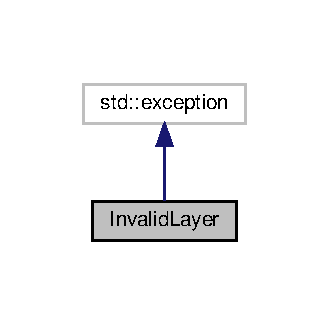
\includegraphics[width=158pt]{classInvalidLayer__inherit__graph}
\end{center}
\end{figure}


Collaboration diagram for Invalid\+Layer\+:
\nopagebreak
\begin{figure}[H]
\begin{center}
\leavevmode
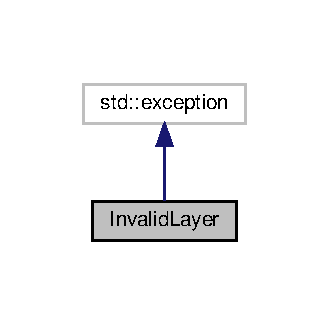
\includegraphics[width=158pt]{classInvalidLayer__coll__graph}
\end{center}
\end{figure}
\subsection*{Public Member Functions}
\begin{DoxyCompactItemize}
\item 
\mbox{\Hypertarget{classInvalidLayer_a2c41dc438799b806f908ccd5c8bae995}\label{classInvalidLayer_a2c41dc438799b806f908ccd5c8bae995}} 
{\bfseries Invalid\+Layer} (const std\+::string \&layer\+Type)
\item 
\mbox{\Hypertarget{classInvalidLayer_a83e01dd706508bf237bb77b0dcc1d76d}\label{classInvalidLayer_a83e01dd706508bf237bb77b0dcc1d76d}} 
const char $\ast$ {\bfseries what} () const  throw ()
\end{DoxyCompactItemize}


The documentation for this class was generated from the following file\+:\begin{DoxyCompactItemize}
\item 
src/tools/json/J\+S\+O\+N\+Model.\+h\end{DoxyCompactItemize}

\hypertarget{structnlohmann_1_1detail_1_1is__basic__json}{}\section{nlohmann\+:\+:detail\+:\+:is\+\_\+basic\+\_\+json$<$ typename $>$ Struct Template Reference}
\label{structnlohmann_1_1detail_1_1is__basic__json}\index{nlohmann\+::detail\+::is\+\_\+basic\+\_\+json$<$ typename $>$@{nlohmann\+::detail\+::is\+\_\+basic\+\_\+json$<$ typename $>$}}


Inheritance diagram for nlohmann\+:\+:detail\+:\+:is\+\_\+basic\+\_\+json$<$ typename $>$\+:
\nopagebreak
\begin{figure}[H]
\begin{center}
\leavevmode
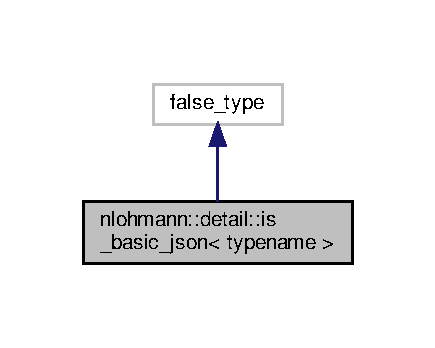
\includegraphics[width=209pt]{structnlohmann_1_1detail_1_1is__basic__json__inherit__graph}
\end{center}
\end{figure}


Collaboration diagram for nlohmann\+:\+:detail\+:\+:is\+\_\+basic\+\_\+json$<$ typename $>$\+:
\nopagebreak
\begin{figure}[H]
\begin{center}
\leavevmode
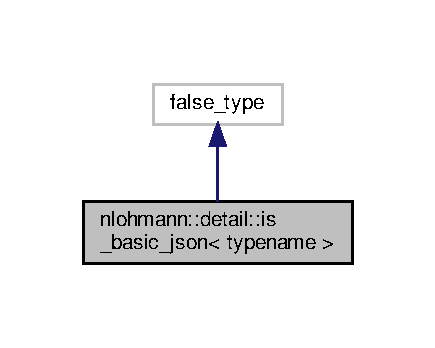
\includegraphics[width=209pt]{structnlohmann_1_1detail_1_1is__basic__json__coll__graph}
\end{center}
\end{figure}


The documentation for this struct was generated from the following file\+:\begin{DoxyCompactItemize}
\item 
src/tools/json/json.\+hpp\end{DoxyCompactItemize}

\hypertarget{structnlohmann_1_1detail_1_1is__basic__json_3_01NLOHMANN__BASIC__JSON__TPL_01_4}{}\section{nlohmann\+:\+:detail\+:\+:is\+\_\+basic\+\_\+json$<$ N\+L\+O\+H\+M\+A\+N\+N\+\_\+\+B\+A\+S\+I\+C\+\_\+\+J\+S\+O\+N\+\_\+\+T\+PL $>$ Struct Reference}
\label{structnlohmann_1_1detail_1_1is__basic__json_3_01NLOHMANN__BASIC__JSON__TPL_01_4}\index{nlohmann\+::detail\+::is\+\_\+basic\+\_\+json$<$ N\+L\+O\+H\+M\+A\+N\+N\+\_\+\+B\+A\+S\+I\+C\+\_\+\+J\+S\+O\+N\+\_\+\+T\+P\+L $>$@{nlohmann\+::detail\+::is\+\_\+basic\+\_\+json$<$ N\+L\+O\+H\+M\+A\+N\+N\+\_\+\+B\+A\+S\+I\+C\+\_\+\+J\+S\+O\+N\+\_\+\+T\+P\+L $>$}}


Inheritance diagram for nlohmann\+:\+:detail\+:\+:is\+\_\+basic\+\_\+json$<$ N\+L\+O\+H\+M\+A\+N\+N\+\_\+\+B\+A\+S\+I\+C\+\_\+\+J\+S\+O\+N\+\_\+\+T\+PL $>$\+:
\nopagebreak
\begin{figure}[H]
\begin{center}
\leavevmode
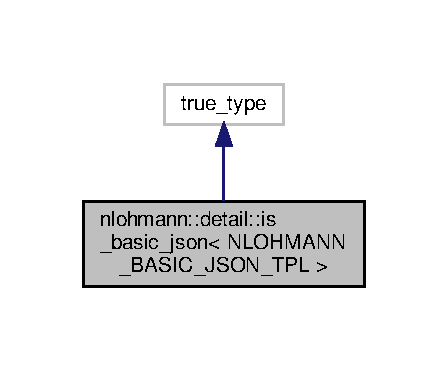
\includegraphics[width=215pt]{structnlohmann_1_1detail_1_1is__basic__json_3_01NLOHMANN__BASIC__JSON__TPL_01_4__inherit__graph}
\end{center}
\end{figure}


Collaboration diagram for nlohmann\+:\+:detail\+:\+:is\+\_\+basic\+\_\+json$<$ N\+L\+O\+H\+M\+A\+N\+N\+\_\+\+B\+A\+S\+I\+C\+\_\+\+J\+S\+O\+N\+\_\+\+T\+PL $>$\+:
\nopagebreak
\begin{figure}[H]
\begin{center}
\leavevmode
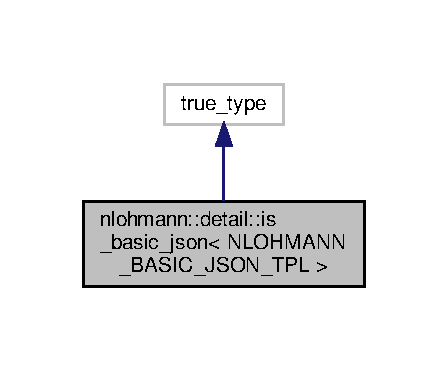
\includegraphics[width=215pt]{structnlohmann_1_1detail_1_1is__basic__json_3_01NLOHMANN__BASIC__JSON__TPL_01_4__coll__graph}
\end{center}
\end{figure}


The documentation for this struct was generated from the following file\+:\begin{DoxyCompactItemize}
\item 
src/tools/json/json.\+hpp\end{DoxyCompactItemize}

\hypertarget{structnlohmann_1_1detail_1_1is__compatible__array__type}{}\section{nlohmann\+:\+:detail\+:\+:is\+\_\+compatible\+\_\+array\+\_\+type$<$ Basic\+Json\+Type, Compatible\+Array\+Type $>$ Struct Template Reference}
\label{structnlohmann_1_1detail_1_1is__compatible__array__type}\index{nlohmann\+::detail\+::is\+\_\+compatible\+\_\+array\+\_\+type$<$ Basic\+Json\+Type, Compatible\+Array\+Type $>$@{nlohmann\+::detail\+::is\+\_\+compatible\+\_\+array\+\_\+type$<$ Basic\+Json\+Type, Compatible\+Array\+Type $>$}}


Inheritance diagram for nlohmann\+:\+:detail\+:\+:is\+\_\+compatible\+\_\+array\+\_\+type$<$ Basic\+Json\+Type, Compatible\+Array\+Type $>$\+:
\nopagebreak
\begin{figure}[H]
\begin{center}
\leavevmode
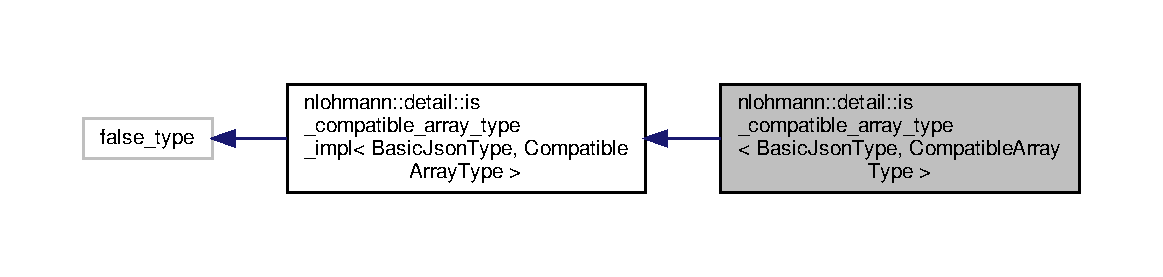
\includegraphics[width=350pt]{structnlohmann_1_1detail_1_1is__compatible__array__type__inherit__graph}
\end{center}
\end{figure}


Collaboration diagram for nlohmann\+:\+:detail\+:\+:is\+\_\+compatible\+\_\+array\+\_\+type$<$ Basic\+Json\+Type, Compatible\+Array\+Type $>$\+:
\nopagebreak
\begin{figure}[H]
\begin{center}
\leavevmode
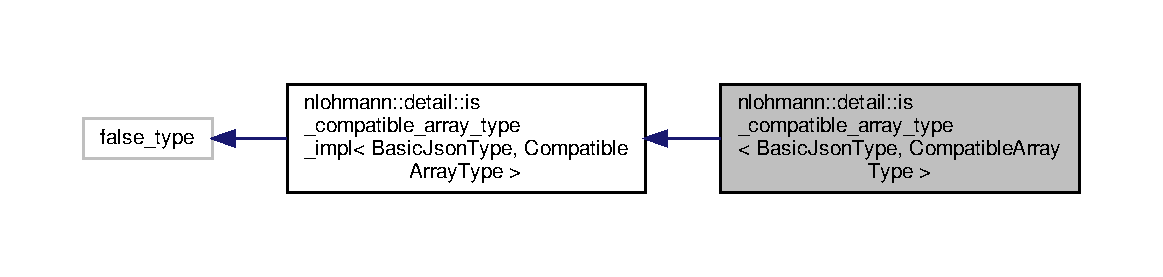
\includegraphics[width=350pt]{structnlohmann_1_1detail_1_1is__compatible__array__type__coll__graph}
\end{center}
\end{figure}


The documentation for this struct was generated from the following file\+:\begin{DoxyCompactItemize}
\item 
src/tools/json/json.\+hpp\end{DoxyCompactItemize}

\hypertarget{structnlohmann_1_1detail_1_1is__compatible__array__type__impl}{}\section{nlohmann\+:\+:detail\+:\+:is\+\_\+compatible\+\_\+array\+\_\+type\+\_\+impl$<$ Basic\+Json\+Type, Compatible\+Array\+Type, typename $>$ Struct Template Reference}
\label{structnlohmann_1_1detail_1_1is__compatible__array__type__impl}\index{nlohmann\+::detail\+::is\+\_\+compatible\+\_\+array\+\_\+type\+\_\+impl$<$ Basic\+Json\+Type, Compatible\+Array\+Type, typename $>$@{nlohmann\+::detail\+::is\+\_\+compatible\+\_\+array\+\_\+type\+\_\+impl$<$ Basic\+Json\+Type, Compatible\+Array\+Type, typename $>$}}


Inheritance diagram for nlohmann\+:\+:detail\+:\+:is\+\_\+compatible\+\_\+array\+\_\+type\+\_\+impl$<$ Basic\+Json\+Type, Compatible\+Array\+Type, typename $>$\+:
\nopagebreak
\begin{figure}[H]
\begin{center}
\leavevmode
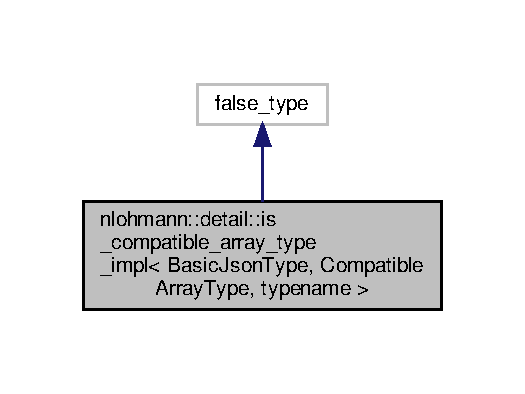
\includegraphics[width=252pt]{structnlohmann_1_1detail_1_1is__compatible__array__type__impl__inherit__graph}
\end{center}
\end{figure}


Collaboration diagram for nlohmann\+:\+:detail\+:\+:is\+\_\+compatible\+\_\+array\+\_\+type\+\_\+impl$<$ Basic\+Json\+Type, Compatible\+Array\+Type, typename $>$\+:
\nopagebreak
\begin{figure}[H]
\begin{center}
\leavevmode
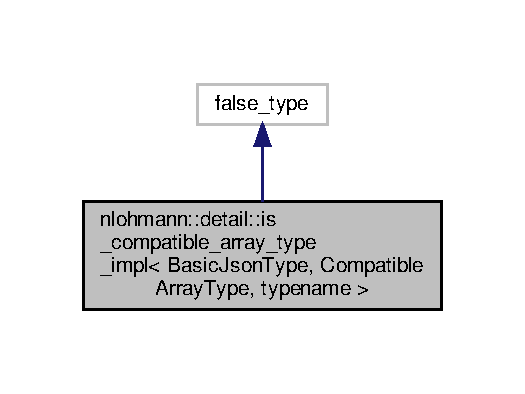
\includegraphics[width=252pt]{structnlohmann_1_1detail_1_1is__compatible__array__type__impl__coll__graph}
\end{center}
\end{figure}


The documentation for this struct was generated from the following file\+:\begin{DoxyCompactItemize}
\item 
src/tools/json/json.\+hpp\end{DoxyCompactItemize}

\hypertarget{structnlohmann_1_1detail_1_1is__compatible__array__type__impl_3_01BasicJsonType_00_01CompatibleA2ae7cc020294dfcc2b3bca5a9db30ddf}{}\section{nlohmann\+:\+:detail\+:\+:is\+\_\+compatible\+\_\+array\+\_\+type\+\_\+impl$<$ Basic\+Json\+Type, Compatible\+Array\+Type, enable\+\_\+if\+\_\+t$<$ is\+\_\+detected$<$ value\+\_\+type\+\_\+t, Compatible\+Array\+Type $>$\+:\+:value and is\+\_\+detected$<$ iterator\+\_\+t, Compatible\+Array\+Type $>$\+:\+:value and not is\+\_\+iterator\+\_\+traits$<$ iterator\+\_\+traits$<$ Compatible\+Array\+Type $>$ $>$\+:\+:value $>$ $>$ Struct Template Reference}
\label{structnlohmann_1_1detail_1_1is__compatible__array__type__impl_3_01BasicJsonType_00_01CompatibleA2ae7cc020294dfcc2b3bca5a9db30ddf}\index{nlohmann\+::detail\+::is\+\_\+compatible\+\_\+array\+\_\+type\+\_\+impl$<$ Basic\+Json\+Type, Compatible\+Array\+Type, enable\+\_\+if\+\_\+t$<$ is\+\_\+detected$<$ value\+\_\+type\+\_\+t, Compatible\+Array\+Type $>$\+::value and is\+\_\+detected$<$ iterator\+\_\+t, Compatible\+Array\+Type $>$\+::value and not is\+\_\+iterator\+\_\+traits$<$ iterator\+\_\+traits$<$ Compatible\+Array\+Type $>$ $>$\+::value $>$ $>$@{nlohmann\+::detail\+::is\+\_\+compatible\+\_\+array\+\_\+type\+\_\+impl$<$ Basic\+Json\+Type, Compatible\+Array\+Type, enable\+\_\+if\+\_\+t$<$ is\+\_\+detected$<$ value\+\_\+type\+\_\+t, Compatible\+Array\+Type $>$\+::value and is\+\_\+detected$<$ iterator\+\_\+t, Compatible\+Array\+Type $>$\+::value and not is\+\_\+iterator\+\_\+traits$<$ iterator\+\_\+traits$<$ Compatible\+Array\+Type $>$ $>$\+::value $>$ $>$}}
\subsection*{Static Public Attributes}
\begin{DoxyCompactItemize}
\item 
static constexpr bool {\bfseries value}
\end{DoxyCompactItemize}


\subsection{Member Data Documentation}
\mbox{\Hypertarget{structnlohmann_1_1detail_1_1is__compatible__array__type__impl_3_01BasicJsonType_00_01CompatibleA2ae7cc020294dfcc2b3bca5a9db30ddf_aa9bdf31f85ac3ee17180a008f1cb81f7}\label{structnlohmann_1_1detail_1_1is__compatible__array__type__impl_3_01BasicJsonType_00_01CompatibleA2ae7cc020294dfcc2b3bca5a9db30ddf_aa9bdf31f85ac3ee17180a008f1cb81f7}} 
\index{nlohmann\+::detail\+::is\+\_\+compatible\+\_\+array\+\_\+type\+\_\+impl$<$ Basic\+Json\+Type, Compatible\+Array\+Type, enable\+\_\+if\+\_\+t$<$ is\+\_\+detected$<$ value\+\_\+type\+\_\+t, Compatible\+Array\+Type $>$\+::value and is\+\_\+detected$<$ iterator\+\_\+t, Compatible\+Array\+Type $>$\+::value and not is\+\_\+iterator\+\_\+traits$<$ iterator\+\_\+traits$<$ Compatible\+Array\+Type $>$ $>$\+::value $>$ $>$@{nlohmann\+::detail\+::is\+\_\+compatible\+\_\+array\+\_\+type\+\_\+impl$<$ Basic\+Json\+Type, Compatible\+Array\+Type, enable\+\_\+if\+\_\+t$<$ is\+\_\+detected$<$ value\+\_\+type\+\_\+t, Compatible\+Array\+Type $>$\+::value and is\+\_\+detected$<$ iterator\+\_\+t, Compatible\+Array\+Type $>$\+::value and not is\+\_\+iterator\+\_\+traits$<$ iterator\+\_\+traits$<$ Compatible\+Array\+Type $>$ $>$\+::value $>$ $>$}!value@{value}}
\index{value@{value}!nlohmann\+::detail\+::is\+\_\+compatible\+\_\+array\+\_\+type\+\_\+impl$<$ Basic\+Json\+Type, Compatible\+Array\+Type, enable\+\_\+if\+\_\+t$<$ is\+\_\+detected$<$ value\+\_\+type\+\_\+t, Compatible\+Array\+Type $>$\+::value and is\+\_\+detected$<$ iterator\+\_\+t, Compatible\+Array\+Type $>$\+::value and not is\+\_\+iterator\+\_\+traits$<$ iterator\+\_\+traits$<$ Compatible\+Array\+Type $>$ $>$\+::value $>$ $>$@{nlohmann\+::detail\+::is\+\_\+compatible\+\_\+array\+\_\+type\+\_\+impl$<$ Basic\+Json\+Type, Compatible\+Array\+Type, enable\+\_\+if\+\_\+t$<$ is\+\_\+detected$<$ value\+\_\+type\+\_\+t, Compatible\+Array\+Type $>$\+::value and is\+\_\+detected$<$ iterator\+\_\+t, Compatible\+Array\+Type $>$\+::value and not is\+\_\+iterator\+\_\+traits$<$ iterator\+\_\+traits$<$ Compatible\+Array\+Type $>$ $>$\+::value $>$ $>$}}
\subsubsection{\texorpdfstring{value}{value}}
{\footnotesize\ttfamily template$<$typename Basic\+Json\+Type , typename Compatible\+Array\+Type $>$ \\
constexpr bool \hyperlink{structnlohmann_1_1detail_1_1is__compatible__array__type__impl}{nlohmann\+::detail\+::is\+\_\+compatible\+\_\+array\+\_\+type\+\_\+impl}$<$ Basic\+Json\+Type, Compatible\+Array\+Type, enable\+\_\+if\+\_\+t$<$ is\+\_\+detected$<$ value\+\_\+type\+\_\+t, Compatible\+Array\+Type $>$\+::value and is\+\_\+detected$<$ iterator\+\_\+t, Compatible\+Array\+Type $>$\+::value and not \hyperlink{structnlohmann_1_1detail_1_1is__iterator__traits}{is\+\_\+iterator\+\_\+traits}$<$ \hyperlink{structnlohmann_1_1detail_1_1iterator__traits}{iterator\+\_\+traits}$<$ Compatible\+Array\+Type $>$ $>$\+::value $>$ $>$\+::value\hspace{0.3cm}{\ttfamily [static]}}

{\bfseries Initial value\+:}
\begin{DoxyCode}
=
        std::is\_constructible<BasicJsonType,
        \textcolor{keyword}{typename} CompatibleArrayType::value\_type>::value
\end{DoxyCode}


The documentation for this struct was generated from the following file\+:\begin{DoxyCompactItemize}
\item 
src/tools/json/json.\+hpp\end{DoxyCompactItemize}

\hypertarget{structnlohmann_1_1detail_1_1is__compatible__integer__type}{}\section{nlohmann\+:\+:detail\+:\+:is\+\_\+compatible\+\_\+integer\+\_\+type$<$ Real\+Integer\+Type, Compatible\+Number\+Integer\+Type $>$ Struct Template Reference}
\label{structnlohmann_1_1detail_1_1is__compatible__integer__type}\index{nlohmann\+::detail\+::is\+\_\+compatible\+\_\+integer\+\_\+type$<$ Real\+Integer\+Type, Compatible\+Number\+Integer\+Type $>$@{nlohmann\+::detail\+::is\+\_\+compatible\+\_\+integer\+\_\+type$<$ Real\+Integer\+Type, Compatible\+Number\+Integer\+Type $>$}}


Inheritance diagram for nlohmann\+:\+:detail\+:\+:is\+\_\+compatible\+\_\+integer\+\_\+type$<$ Real\+Integer\+Type, Compatible\+Number\+Integer\+Type $>$\+:
\nopagebreak
\begin{figure}[H]
\begin{center}
\leavevmode
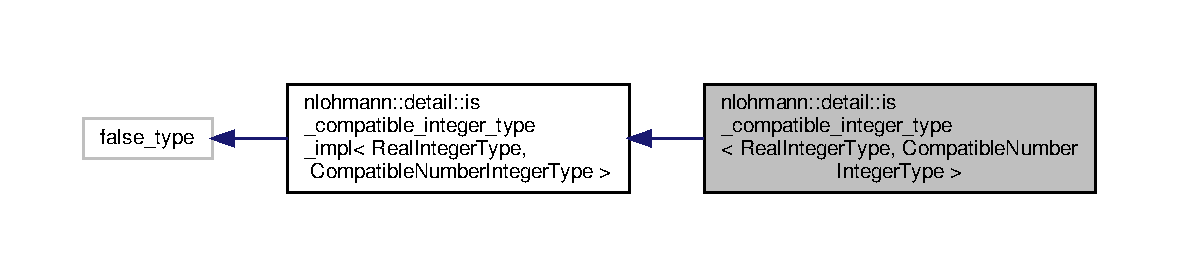
\includegraphics[width=350pt]{structnlohmann_1_1detail_1_1is__compatible__integer__type__inherit__graph}
\end{center}
\end{figure}


Collaboration diagram for nlohmann\+:\+:detail\+:\+:is\+\_\+compatible\+\_\+integer\+\_\+type$<$ Real\+Integer\+Type, Compatible\+Number\+Integer\+Type $>$\+:
\nopagebreak
\begin{figure}[H]
\begin{center}
\leavevmode
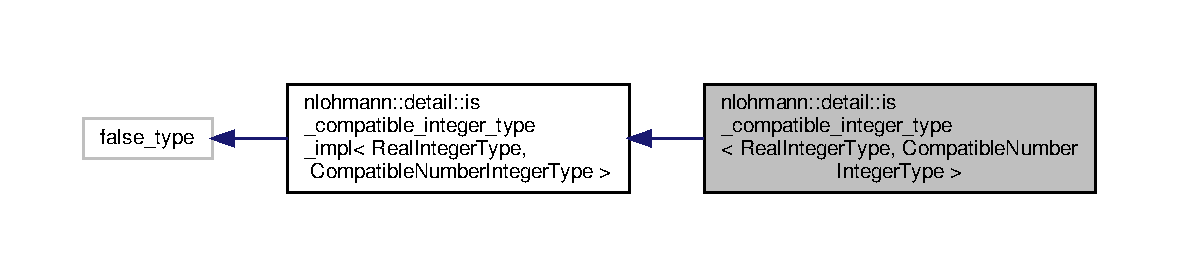
\includegraphics[width=350pt]{structnlohmann_1_1detail_1_1is__compatible__integer__type__coll__graph}
\end{center}
\end{figure}


The documentation for this struct was generated from the following file\+:\begin{DoxyCompactItemize}
\item 
src/tools/json/json.\+hpp\end{DoxyCompactItemize}

\hypertarget{structnlohmann_1_1detail_1_1is__compatible__integer__type__impl}{}\section{nlohmann\+:\+:detail\+:\+:is\+\_\+compatible\+\_\+integer\+\_\+type\+\_\+impl$<$ Real\+Integer\+Type, Compatible\+Number\+Integer\+Type, typename $>$ Struct Template Reference}
\label{structnlohmann_1_1detail_1_1is__compatible__integer__type__impl}\index{nlohmann\+::detail\+::is\+\_\+compatible\+\_\+integer\+\_\+type\+\_\+impl$<$ Real\+Integer\+Type, Compatible\+Number\+Integer\+Type, typename $>$@{nlohmann\+::detail\+::is\+\_\+compatible\+\_\+integer\+\_\+type\+\_\+impl$<$ Real\+Integer\+Type, Compatible\+Number\+Integer\+Type, typename $>$}}


Inheritance diagram for nlohmann\+:\+:detail\+:\+:is\+\_\+compatible\+\_\+integer\+\_\+type\+\_\+impl$<$ Real\+Integer\+Type, Compatible\+Number\+Integer\+Type, typename $>$\+:
\nopagebreak
\begin{figure}[H]
\begin{center}
\leavevmode
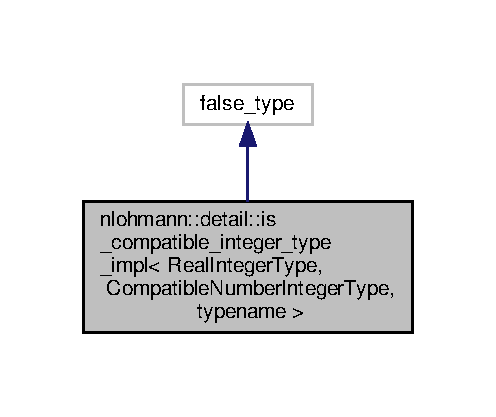
\includegraphics[width=238pt]{structnlohmann_1_1detail_1_1is__compatible__integer__type__impl__inherit__graph}
\end{center}
\end{figure}


Collaboration diagram for nlohmann\+:\+:detail\+:\+:is\+\_\+compatible\+\_\+integer\+\_\+type\+\_\+impl$<$ Real\+Integer\+Type, Compatible\+Number\+Integer\+Type, typename $>$\+:
\nopagebreak
\begin{figure}[H]
\begin{center}
\leavevmode
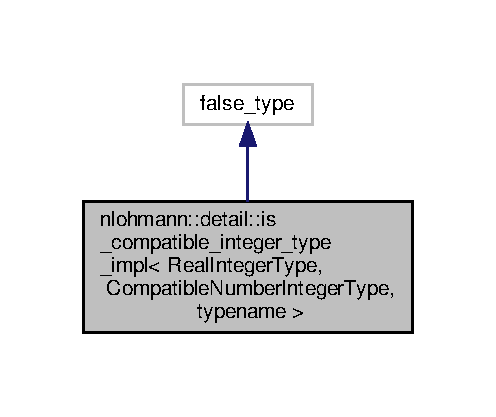
\includegraphics[width=238pt]{structnlohmann_1_1detail_1_1is__compatible__integer__type__impl__coll__graph}
\end{center}
\end{figure}


The documentation for this struct was generated from the following file\+:\begin{DoxyCompactItemize}
\item 
src/tools/json/json.\+hpp\end{DoxyCompactItemize}

\hypertarget{structnlohmann_1_1detail_1_1is__compatible__integer__type__impl_3_01RealIntegerType_00_01Compati3a04243716e8bda67d1ff2aead18da88}{}\section{nlohmann\+:\+:detail\+:\+:is\+\_\+compatible\+\_\+integer\+\_\+type\+\_\+impl$<$ Real\+Integer\+Type, Compatible\+Number\+Integer\+Type, enable\+\_\+if\+\_\+t$<$ std\+:\+:is\+\_\+integral$<$ Real\+Integer\+Type $>$\+:\+:value and std\+:\+:is\+\_\+integral$<$ Compatible\+Number\+Integer\+Type $>$\+:\+:value and not std\+:\+:is\+\_\+same$<$ bool, Compatible\+Number\+Integer\+Type $>$\+:\+:value $>$ $>$ Struct Template Reference}
\label{structnlohmann_1_1detail_1_1is__compatible__integer__type__impl_3_01RealIntegerType_00_01Compati3a04243716e8bda67d1ff2aead18da88}\index{nlohmann\+::detail\+::is\+\_\+compatible\+\_\+integer\+\_\+type\+\_\+impl$<$ Real\+Integer\+Type, Compatible\+Number\+Integer\+Type, enable\+\_\+if\+\_\+t$<$ std\+::is\+\_\+integral$<$ Real\+Integer\+Type $>$\+::value and std\+::is\+\_\+integral$<$ Compatible\+Number\+Integer\+Type $>$\+::value and not std\+::is\+\_\+same$<$ bool, Compatible\+Number\+Integer\+Type $>$\+::value $>$ $>$@{nlohmann\+::detail\+::is\+\_\+compatible\+\_\+integer\+\_\+type\+\_\+impl$<$ Real\+Integer\+Type, Compatible\+Number\+Integer\+Type, enable\+\_\+if\+\_\+t$<$ std\+::is\+\_\+integral$<$ Real\+Integer\+Type $>$\+::value and std\+::is\+\_\+integral$<$ Compatible\+Number\+Integer\+Type $>$\+::value and not std\+::is\+\_\+same$<$ bool, Compatible\+Number\+Integer\+Type $>$\+::value $>$ $>$}}
\subsection*{Public Types}
\begin{DoxyCompactItemize}
\item 
\mbox{\Hypertarget{structnlohmann_1_1detail_1_1is__compatible__integer__type__impl_3_01RealIntegerType_00_01Compati3a04243716e8bda67d1ff2aead18da88_a0e9f2586c4de25750563770c9388ab9f}\label{structnlohmann_1_1detail_1_1is__compatible__integer__type__impl_3_01RealIntegerType_00_01Compati3a04243716e8bda67d1ff2aead18da88_a0e9f2586c4de25750563770c9388ab9f}} 
using {\bfseries Real\+Limits} = std\+::numeric\+\_\+limits$<$ Real\+Integer\+Type $>$
\item 
\mbox{\Hypertarget{structnlohmann_1_1detail_1_1is__compatible__integer__type__impl_3_01RealIntegerType_00_01Compati3a04243716e8bda67d1ff2aead18da88_a002983b5c7c0f72b89d2151a6b39627d}\label{structnlohmann_1_1detail_1_1is__compatible__integer__type__impl_3_01RealIntegerType_00_01Compati3a04243716e8bda67d1ff2aead18da88_a002983b5c7c0f72b89d2151a6b39627d}} 
using {\bfseries Compatible\+Limits} = std\+::numeric\+\_\+limits$<$ Compatible\+Number\+Integer\+Type $>$
\end{DoxyCompactItemize}
\subsection*{Static Public Attributes}
\begin{DoxyCompactItemize}
\item 
static constexpr auto {\bfseries value}
\end{DoxyCompactItemize}


\subsection{Member Data Documentation}
\mbox{\Hypertarget{structnlohmann_1_1detail_1_1is__compatible__integer__type__impl_3_01RealIntegerType_00_01Compati3a04243716e8bda67d1ff2aead18da88_a478242daac7a70e28c749bfec00d1c1b}\label{structnlohmann_1_1detail_1_1is__compatible__integer__type__impl_3_01RealIntegerType_00_01Compati3a04243716e8bda67d1ff2aead18da88_a478242daac7a70e28c749bfec00d1c1b}} 
\index{nlohmann\+::detail\+::is\+\_\+compatible\+\_\+integer\+\_\+type\+\_\+impl$<$ Real\+Integer\+Type, Compatible\+Number\+Integer\+Type, enable\+\_\+if\+\_\+t$<$ std\+::is\+\_\+integral$<$ Real\+Integer\+Type $>$\+::value and std\+::is\+\_\+integral$<$ Compatible\+Number\+Integer\+Type $>$\+::value and not std\+::is\+\_\+same$<$ bool, Compatible\+Number\+Integer\+Type $>$\+::value $>$ $>$@{nlohmann\+::detail\+::is\+\_\+compatible\+\_\+integer\+\_\+type\+\_\+impl$<$ Real\+Integer\+Type, Compatible\+Number\+Integer\+Type, enable\+\_\+if\+\_\+t$<$ std\+::is\+\_\+integral$<$ Real\+Integer\+Type $>$\+::value and std\+::is\+\_\+integral$<$ Compatible\+Number\+Integer\+Type $>$\+::value and not std\+::is\+\_\+same$<$ bool, Compatible\+Number\+Integer\+Type $>$\+::value $>$ $>$}!value@{value}}
\index{value@{value}!nlohmann\+::detail\+::is\+\_\+compatible\+\_\+integer\+\_\+type\+\_\+impl$<$ Real\+Integer\+Type, Compatible\+Number\+Integer\+Type, enable\+\_\+if\+\_\+t$<$ std\+::is\+\_\+integral$<$ Real\+Integer\+Type $>$\+::value and std\+::is\+\_\+integral$<$ Compatible\+Number\+Integer\+Type $>$\+::value and not std\+::is\+\_\+same$<$ bool, Compatible\+Number\+Integer\+Type $>$\+::value $>$ $>$@{nlohmann\+::detail\+::is\+\_\+compatible\+\_\+integer\+\_\+type\+\_\+impl$<$ Real\+Integer\+Type, Compatible\+Number\+Integer\+Type, enable\+\_\+if\+\_\+t$<$ std\+::is\+\_\+integral$<$ Real\+Integer\+Type $>$\+::value and std\+::is\+\_\+integral$<$ Compatible\+Number\+Integer\+Type $>$\+::value and not std\+::is\+\_\+same$<$ bool, Compatible\+Number\+Integer\+Type $>$\+::value $>$ $>$}}
\subsubsection{\texorpdfstring{value}{value}}
{\footnotesize\ttfamily template$<$typename Real\+Integer\+Type , typename Compatible\+Number\+Integer\+Type $>$ \\
constexpr auto \hyperlink{structnlohmann_1_1detail_1_1is__compatible__integer__type__impl}{nlohmann\+::detail\+::is\+\_\+compatible\+\_\+integer\+\_\+type\+\_\+impl}$<$ Real\+Integer\+Type, Compatible\+Number\+Integer\+Type, enable\+\_\+if\+\_\+t$<$ std\+::is\+\_\+integral$<$ Real\+Integer\+Type $>$\+::value and std\+::is\+\_\+integral$<$ Compatible\+Number\+Integer\+Type $>$\+::value and not std\+::is\+\_\+same$<$ bool, Compatible\+Number\+Integer\+Type $>$\+::value $>$ $>$\+::value\hspace{0.3cm}{\ttfamily [static]}}

{\bfseries Initial value\+:}
\begin{DoxyCode}
=
        std::is\_constructible<RealIntegerType,
        CompatibleNumberIntegerType>::value and
        CompatibleLimits::is\_integer and
        RealLimits::is\_signed == CompatibleLimits::is\_signed
\end{DoxyCode}


The documentation for this struct was generated from the following file\+:\begin{DoxyCompactItemize}
\item 
src/tools/json/json.\+hpp\end{DoxyCompactItemize}

\hypertarget{structnlohmann_1_1detail_1_1is__compatible__object__type}{}\section{nlohmann\+:\+:detail\+:\+:is\+\_\+compatible\+\_\+object\+\_\+type$<$ Basic\+Json\+Type, Compatible\+Object\+Type $>$ Struct Template Reference}
\label{structnlohmann_1_1detail_1_1is__compatible__object__type}\index{nlohmann\+::detail\+::is\+\_\+compatible\+\_\+object\+\_\+type$<$ Basic\+Json\+Type, Compatible\+Object\+Type $>$@{nlohmann\+::detail\+::is\+\_\+compatible\+\_\+object\+\_\+type$<$ Basic\+Json\+Type, Compatible\+Object\+Type $>$}}


Inheritance diagram for nlohmann\+:\+:detail\+:\+:is\+\_\+compatible\+\_\+object\+\_\+type$<$ Basic\+Json\+Type, Compatible\+Object\+Type $>$\+:
\nopagebreak
\begin{figure}[H]
\begin{center}
\leavevmode
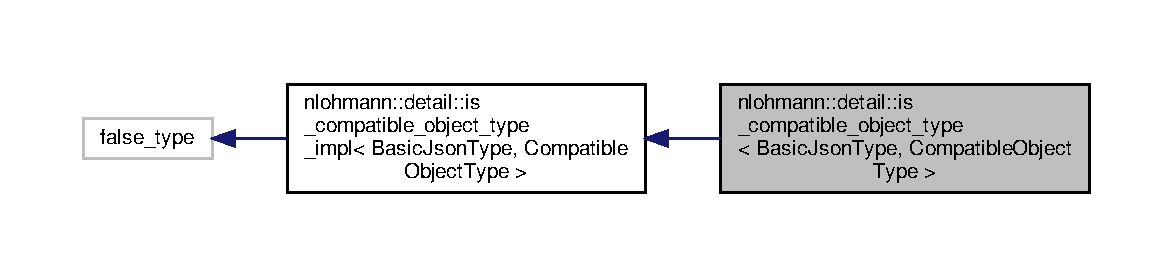
\includegraphics[width=350pt]{structnlohmann_1_1detail_1_1is__compatible__object__type__inherit__graph}
\end{center}
\end{figure}


Collaboration diagram for nlohmann\+:\+:detail\+:\+:is\+\_\+compatible\+\_\+object\+\_\+type$<$ Basic\+Json\+Type, Compatible\+Object\+Type $>$\+:
\nopagebreak
\begin{figure}[H]
\begin{center}
\leavevmode
\includegraphics[width=350pt]{structnlohmann_1_1detail_1_1is__compatible__object__type__coll__graph}
\end{center}
\end{figure}


The documentation for this struct was generated from the following file\+:\begin{DoxyCompactItemize}
\item 
src/tools/json/json.\+hpp\end{DoxyCompactItemize}

\hypertarget{structnlohmann_1_1detail_1_1is__compatible__object__type__impl}{}\section{nlohmann\+:\+:detail\+:\+:is\+\_\+compatible\+\_\+object\+\_\+type\+\_\+impl$<$ Basic\+Json\+Type, Compatible\+Object\+Type, typename $>$ Struct Template Reference}
\label{structnlohmann_1_1detail_1_1is__compatible__object__type__impl}\index{nlohmann\+::detail\+::is\+\_\+compatible\+\_\+object\+\_\+type\+\_\+impl$<$ Basic\+Json\+Type, Compatible\+Object\+Type, typename $>$@{nlohmann\+::detail\+::is\+\_\+compatible\+\_\+object\+\_\+type\+\_\+impl$<$ Basic\+Json\+Type, Compatible\+Object\+Type, typename $>$}}


Inheritance diagram for nlohmann\+:\+:detail\+:\+:is\+\_\+compatible\+\_\+object\+\_\+type\+\_\+impl$<$ Basic\+Json\+Type, Compatible\+Object\+Type, typename $>$\+:
\nopagebreak
\begin{figure}[H]
\begin{center}
\leavevmode
\includegraphics[width=252pt]{structnlohmann_1_1detail_1_1is__compatible__object__type__impl__inherit__graph}
\end{center}
\end{figure}


Collaboration diagram for nlohmann\+:\+:detail\+:\+:is\+\_\+compatible\+\_\+object\+\_\+type\+\_\+impl$<$ Basic\+Json\+Type, Compatible\+Object\+Type, typename $>$\+:
\nopagebreak
\begin{figure}[H]
\begin{center}
\leavevmode
\includegraphics[width=252pt]{structnlohmann_1_1detail_1_1is__compatible__object__type__impl__coll__graph}
\end{center}
\end{figure}


The documentation for this struct was generated from the following file\+:\begin{DoxyCompactItemize}
\item 
src/tools/json/json.\+hpp\end{DoxyCompactItemize}

\hypertarget{structnlohmann_1_1detail_1_1is__compatible__object__type__impl_3_01BasicJsonType_00_01Compatible0bd988932da161d60568f9b7198a50d2}{}\section{nlohmann\+:\+:detail\+:\+:is\+\_\+compatible\+\_\+object\+\_\+type\+\_\+impl$<$ Basic\+Json\+Type, Compatible\+Object\+Type, enable\+\_\+if\+\_\+t$<$ is\+\_\+detected$<$ mapped\+\_\+type\+\_\+t, Compatible\+Object\+Type $>$\+:\+:value and is\+\_\+detected$<$ key\+\_\+type\+\_\+t, Compatible\+Object\+Type $>$\+:\+:value $>$ $>$ Struct Template Reference}
\label{structnlohmann_1_1detail_1_1is__compatible__object__type__impl_3_01BasicJsonType_00_01Compatible0bd988932da161d60568f9b7198a50d2}\index{nlohmann\+::detail\+::is\+\_\+compatible\+\_\+object\+\_\+type\+\_\+impl$<$ Basic\+Json\+Type, Compatible\+Object\+Type, enable\+\_\+if\+\_\+t$<$ is\+\_\+detected$<$ mapped\+\_\+type\+\_\+t, Compatible\+Object\+Type $>$\+::value and is\+\_\+detected$<$ key\+\_\+type\+\_\+t, Compatible\+Object\+Type $>$\+::value $>$ $>$@{nlohmann\+::detail\+::is\+\_\+compatible\+\_\+object\+\_\+type\+\_\+impl$<$ Basic\+Json\+Type, Compatible\+Object\+Type, enable\+\_\+if\+\_\+t$<$ is\+\_\+detected$<$ mapped\+\_\+type\+\_\+t, Compatible\+Object\+Type $>$\+::value and is\+\_\+detected$<$ key\+\_\+type\+\_\+t, Compatible\+Object\+Type $>$\+::value $>$ $>$}}
\subsection*{Public Types}
\begin{DoxyCompactItemize}
\item 
\mbox{\Hypertarget{structnlohmann_1_1detail_1_1is__compatible__object__type__impl_3_01BasicJsonType_00_01Compatible0bd988932da161d60568f9b7198a50d2_a551e9ee372c1b24b632e6b668c231a62}\label{structnlohmann_1_1detail_1_1is__compatible__object__type__impl_3_01BasicJsonType_00_01Compatible0bd988932da161d60568f9b7198a50d2_a551e9ee372c1b24b632e6b668c231a62}} 
using {\bfseries object\+\_\+t} = typename Basic\+Json\+Type\+::object\+\_\+t
\end{DoxyCompactItemize}
\subsection*{Static Public Attributes}
\begin{DoxyCompactItemize}
\item 
static constexpr bool {\bfseries value}
\end{DoxyCompactItemize}


\subsection{Member Data Documentation}
\mbox{\Hypertarget{structnlohmann_1_1detail_1_1is__compatible__object__type__impl_3_01BasicJsonType_00_01Compatible0bd988932da161d60568f9b7198a50d2_adc8188ae8d65e8175d961cd461a8ee43}\label{structnlohmann_1_1detail_1_1is__compatible__object__type__impl_3_01BasicJsonType_00_01Compatible0bd988932da161d60568f9b7198a50d2_adc8188ae8d65e8175d961cd461a8ee43}} 
\index{nlohmann\+::detail\+::is\+\_\+compatible\+\_\+object\+\_\+type\+\_\+impl$<$ Basic\+Json\+Type, Compatible\+Object\+Type, enable\+\_\+if\+\_\+t$<$ is\+\_\+detected$<$ mapped\+\_\+type\+\_\+t, Compatible\+Object\+Type $>$\+::value and is\+\_\+detected$<$ key\+\_\+type\+\_\+t, Compatible\+Object\+Type $>$\+::value $>$ $>$@{nlohmann\+::detail\+::is\+\_\+compatible\+\_\+object\+\_\+type\+\_\+impl$<$ Basic\+Json\+Type, Compatible\+Object\+Type, enable\+\_\+if\+\_\+t$<$ is\+\_\+detected$<$ mapped\+\_\+type\+\_\+t, Compatible\+Object\+Type $>$\+::value and is\+\_\+detected$<$ key\+\_\+type\+\_\+t, Compatible\+Object\+Type $>$\+::value $>$ $>$}!value@{value}}
\index{value@{value}!nlohmann\+::detail\+::is\+\_\+compatible\+\_\+object\+\_\+type\+\_\+impl$<$ Basic\+Json\+Type, Compatible\+Object\+Type, enable\+\_\+if\+\_\+t$<$ is\+\_\+detected$<$ mapped\+\_\+type\+\_\+t, Compatible\+Object\+Type $>$\+::value and is\+\_\+detected$<$ key\+\_\+type\+\_\+t, Compatible\+Object\+Type $>$\+::value $>$ $>$@{nlohmann\+::detail\+::is\+\_\+compatible\+\_\+object\+\_\+type\+\_\+impl$<$ Basic\+Json\+Type, Compatible\+Object\+Type, enable\+\_\+if\+\_\+t$<$ is\+\_\+detected$<$ mapped\+\_\+type\+\_\+t, Compatible\+Object\+Type $>$\+::value and is\+\_\+detected$<$ key\+\_\+type\+\_\+t, Compatible\+Object\+Type $>$\+::value $>$ $>$}}
\subsubsection{\texorpdfstring{value}{value}}
{\footnotesize\ttfamily template$<$typename Basic\+Json\+Type , typename Compatible\+Object\+Type $>$ \\
constexpr bool \hyperlink{structnlohmann_1_1detail_1_1is__compatible__object__type__impl}{nlohmann\+::detail\+::is\+\_\+compatible\+\_\+object\+\_\+type\+\_\+impl}$<$ Basic\+Json\+Type, Compatible\+Object\+Type, enable\+\_\+if\+\_\+t$<$ is\+\_\+detected$<$ mapped\+\_\+type\+\_\+t, Compatible\+Object\+Type $>$\+::value and is\+\_\+detected$<$ key\+\_\+type\+\_\+t, Compatible\+Object\+Type $>$\+::value $>$ $>$\+::value\hspace{0.3cm}{\ttfamily [static]}}

{\bfseries Initial value\+:}
\begin{DoxyCode}
=
        std::is\_constructible<\textcolor{keyword}{typename} object\_t::key\_type,
        \textcolor{keyword}{typename} CompatibleObjectType::key\_type>::value and
        std::is\_constructible<\textcolor{keyword}{typename} object\_t::mapped\_type,
        \textcolor{keyword}{typename} CompatibleObjectType::mapped\_type>::value
\end{DoxyCode}


The documentation for this struct was generated from the following file\+:\begin{DoxyCompactItemize}
\item 
src/tools/json/json.\+hpp\end{DoxyCompactItemize}

\hypertarget{structnlohmann_1_1detail_1_1is__compatible__string__type}{}\section{nlohmann\+:\+:detail\+:\+:is\+\_\+compatible\+\_\+string\+\_\+type$<$ Basic\+Json\+Type, Constructible\+String\+Type $>$ Struct Template Reference}
\label{structnlohmann_1_1detail_1_1is__compatible__string__type}\index{nlohmann\+::detail\+::is\+\_\+compatible\+\_\+string\+\_\+type$<$ Basic\+Json\+Type, Constructible\+String\+Type $>$@{nlohmann\+::detail\+::is\+\_\+compatible\+\_\+string\+\_\+type$<$ Basic\+Json\+Type, Constructible\+String\+Type $>$}}


Inheritance diagram for nlohmann\+:\+:detail\+:\+:is\+\_\+compatible\+\_\+string\+\_\+type$<$ Basic\+Json\+Type, Constructible\+String\+Type $>$\+:
\nopagebreak
\begin{figure}[H]
\begin{center}
\leavevmode
\includegraphics[width=350pt]{structnlohmann_1_1detail_1_1is__compatible__string__type__inherit__graph}
\end{center}
\end{figure}


Collaboration diagram for nlohmann\+:\+:detail\+:\+:is\+\_\+compatible\+\_\+string\+\_\+type$<$ Basic\+Json\+Type, Constructible\+String\+Type $>$\+:
\nopagebreak
\begin{figure}[H]
\begin{center}
\leavevmode
\includegraphics[width=350pt]{structnlohmann_1_1detail_1_1is__compatible__string__type__coll__graph}
\end{center}
\end{figure}


The documentation for this struct was generated from the following file\+:\begin{DoxyCompactItemize}
\item 
src/tools/json/json.\+hpp\end{DoxyCompactItemize}

\hypertarget{structnlohmann_1_1detail_1_1is__compatible__string__type__impl}{}\section{nlohmann\+:\+:detail\+:\+:is\+\_\+compatible\+\_\+string\+\_\+type\+\_\+impl$<$ Basic\+Json\+Type, Compatible\+String\+Type, typename $>$ Struct Template Reference}
\label{structnlohmann_1_1detail_1_1is__compatible__string__type__impl}\index{nlohmann\+::detail\+::is\+\_\+compatible\+\_\+string\+\_\+type\+\_\+impl$<$ Basic\+Json\+Type, Compatible\+String\+Type, typename $>$@{nlohmann\+::detail\+::is\+\_\+compatible\+\_\+string\+\_\+type\+\_\+impl$<$ Basic\+Json\+Type, Compatible\+String\+Type, typename $>$}}


Inheritance diagram for nlohmann\+:\+:detail\+:\+:is\+\_\+compatible\+\_\+string\+\_\+type\+\_\+impl$<$ Basic\+Json\+Type, Compatible\+String\+Type, typename $>$\+:
\nopagebreak
\begin{figure}[H]
\begin{center}
\leavevmode
\includegraphics[width=252pt]{structnlohmann_1_1detail_1_1is__compatible__string__type__impl__inherit__graph}
\end{center}
\end{figure}


Collaboration diagram for nlohmann\+:\+:detail\+:\+:is\+\_\+compatible\+\_\+string\+\_\+type\+\_\+impl$<$ Basic\+Json\+Type, Compatible\+String\+Type, typename $>$\+:
\nopagebreak
\begin{figure}[H]
\begin{center}
\leavevmode
\includegraphics[width=252pt]{structnlohmann_1_1detail_1_1is__compatible__string__type__impl__coll__graph}
\end{center}
\end{figure}


The documentation for this struct was generated from the following file\+:\begin{DoxyCompactItemize}
\item 
src/tools/json/json.\+hpp\end{DoxyCompactItemize}

\hypertarget{structnlohmann_1_1detail_1_1is__compatible__string__type__impl_3_01BasicJsonType_00_01Compatible494e9dc742c819c61e54b8282030b5b6}{}\section{nlohmann\+:\+:detail\+:\+:is\+\_\+compatible\+\_\+string\+\_\+type\+\_\+impl$<$ Basic\+Json\+Type, Compatible\+String\+Type, enable\+\_\+if\+\_\+t$<$ is\+\_\+detected\+\_\+exact$<$ typename Basic\+Json\+Type\+:\+:string\+\_\+t\+:\+:value\+\_\+type, value\+\_\+type\+\_\+t, Compatible\+String\+Type $>$\+:\+:value $>$ $>$ Struct Template Reference}
\label{structnlohmann_1_1detail_1_1is__compatible__string__type__impl_3_01BasicJsonType_00_01Compatible494e9dc742c819c61e54b8282030b5b6}\index{nlohmann\+::detail\+::is\+\_\+compatible\+\_\+string\+\_\+type\+\_\+impl$<$ Basic\+Json\+Type, Compatible\+String\+Type, enable\+\_\+if\+\_\+t$<$ is\+\_\+detected\+\_\+exact$<$ typename Basic\+Json\+Type\+::string\+\_\+t\+::value\+\_\+type, value\+\_\+type\+\_\+t, Compatible\+String\+Type $>$\+::value $>$ $>$@{nlohmann\+::detail\+::is\+\_\+compatible\+\_\+string\+\_\+type\+\_\+impl$<$ Basic\+Json\+Type, Compatible\+String\+Type, enable\+\_\+if\+\_\+t$<$ is\+\_\+detected\+\_\+exact$<$ typename Basic\+Json\+Type\+::string\+\_\+t\+::value\+\_\+type, value\+\_\+type\+\_\+t, Compatible\+String\+Type $>$\+::value $>$ $>$}}
\subsection*{Static Public Attributes}
\begin{DoxyCompactItemize}
\item 
static constexpr auto {\bfseries value}
\end{DoxyCompactItemize}


\subsection{Member Data Documentation}
\mbox{\Hypertarget{structnlohmann_1_1detail_1_1is__compatible__string__type__impl_3_01BasicJsonType_00_01Compatible494e9dc742c819c61e54b8282030b5b6_adac1e17a2ddf9ac94be736e96e8943a9}\label{structnlohmann_1_1detail_1_1is__compatible__string__type__impl_3_01BasicJsonType_00_01Compatible494e9dc742c819c61e54b8282030b5b6_adac1e17a2ddf9ac94be736e96e8943a9}} 
\index{nlohmann\+::detail\+::is\+\_\+compatible\+\_\+string\+\_\+type\+\_\+impl$<$ Basic\+Json\+Type, Compatible\+String\+Type, enable\+\_\+if\+\_\+t$<$ is\+\_\+detected\+\_\+exact$<$ typename Basic\+Json\+Type\+::string\+\_\+t\+::value\+\_\+type, value\+\_\+type\+\_\+t, Compatible\+String\+Type $>$\+::value $>$ $>$@{nlohmann\+::detail\+::is\+\_\+compatible\+\_\+string\+\_\+type\+\_\+impl$<$ Basic\+Json\+Type, Compatible\+String\+Type, enable\+\_\+if\+\_\+t$<$ is\+\_\+detected\+\_\+exact$<$ typename Basic\+Json\+Type\+::string\+\_\+t\+::value\+\_\+type, value\+\_\+type\+\_\+t, Compatible\+String\+Type $>$\+::value $>$ $>$}!value@{value}}
\index{value@{value}!nlohmann\+::detail\+::is\+\_\+compatible\+\_\+string\+\_\+type\+\_\+impl$<$ Basic\+Json\+Type, Compatible\+String\+Type, enable\+\_\+if\+\_\+t$<$ is\+\_\+detected\+\_\+exact$<$ typename Basic\+Json\+Type\+::string\+\_\+t\+::value\+\_\+type, value\+\_\+type\+\_\+t, Compatible\+String\+Type $>$\+::value $>$ $>$@{nlohmann\+::detail\+::is\+\_\+compatible\+\_\+string\+\_\+type\+\_\+impl$<$ Basic\+Json\+Type, Compatible\+String\+Type, enable\+\_\+if\+\_\+t$<$ is\+\_\+detected\+\_\+exact$<$ typename Basic\+Json\+Type\+::string\+\_\+t\+::value\+\_\+type, value\+\_\+type\+\_\+t, Compatible\+String\+Type $>$\+::value $>$ $>$}}
\subsubsection{\texorpdfstring{value}{value}}
{\footnotesize\ttfamily template$<$typename Basic\+Json\+Type , typename Compatible\+String\+Type $>$ \\
constexpr auto \hyperlink{structnlohmann_1_1detail_1_1is__compatible__string__type__impl}{nlohmann\+::detail\+::is\+\_\+compatible\+\_\+string\+\_\+type\+\_\+impl}$<$ Basic\+Json\+Type, Compatible\+String\+Type, enable\+\_\+if\+\_\+t$<$ is\+\_\+detected\+\_\+exact$<$ typename Basic\+Json\+Type\+::string\+\_\+t\+::value\+\_\+type, value\+\_\+type\+\_\+t, Compatible\+String\+Type $>$\+::value $>$ $>$\+::value\hspace{0.3cm}{\ttfamily [static]}}

{\bfseries Initial value\+:}
\begin{DoxyCode}
=
        std::is\_constructible<typename BasicJsonType::string\_t, CompatibleStringType>::value
\end{DoxyCode}


The documentation for this struct was generated from the following file\+:\begin{DoxyCompactItemize}
\item 
src/tools/json/json.\+hpp\end{DoxyCompactItemize}

\hypertarget{structnlohmann_1_1detail_1_1is__compatible__type}{}\section{nlohmann\+:\+:detail\+:\+:is\+\_\+compatible\+\_\+type$<$ Basic\+Json\+Type, Compatible\+Type $>$ Struct Template Reference}
\label{structnlohmann_1_1detail_1_1is__compatible__type}\index{nlohmann\+::detail\+::is\+\_\+compatible\+\_\+type$<$ Basic\+Json\+Type, Compatible\+Type $>$@{nlohmann\+::detail\+::is\+\_\+compatible\+\_\+type$<$ Basic\+Json\+Type, Compatible\+Type $>$}}


Inheritance diagram for nlohmann\+:\+:detail\+:\+:is\+\_\+compatible\+\_\+type$<$ Basic\+Json\+Type, Compatible\+Type $>$\+:
\nopagebreak
\begin{figure}[H]
\begin{center}
\leavevmode
\includegraphics[width=259pt]{structnlohmann_1_1detail_1_1is__compatible__type__inherit__graph}
\end{center}
\end{figure}


Collaboration diagram for nlohmann\+:\+:detail\+:\+:is\+\_\+compatible\+\_\+type$<$ Basic\+Json\+Type, Compatible\+Type $>$\+:
\nopagebreak
\begin{figure}[H]
\begin{center}
\leavevmode
\includegraphics[width=259pt]{structnlohmann_1_1detail_1_1is__compatible__type__coll__graph}
\end{center}
\end{figure}


The documentation for this struct was generated from the following file\+:\begin{DoxyCompactItemize}
\item 
src/tools/json/json.\+hpp\end{DoxyCompactItemize}

\hypertarget{structnlohmann_1_1detail_1_1is__compatible__type__impl}{}\section{nlohmann\+:\+:detail\+:\+:is\+\_\+compatible\+\_\+type\+\_\+impl$<$ Basic\+Json\+Type, Compatible\+Type, typename $>$ Struct Template Reference}
\label{structnlohmann_1_1detail_1_1is__compatible__type__impl}\index{nlohmann\+::detail\+::is\+\_\+compatible\+\_\+type\+\_\+impl$<$ Basic\+Json\+Type, Compatible\+Type, typename $>$@{nlohmann\+::detail\+::is\+\_\+compatible\+\_\+type\+\_\+impl$<$ Basic\+Json\+Type, Compatible\+Type, typename $>$}}


Inheritance diagram for nlohmann\+:\+:detail\+:\+:is\+\_\+compatible\+\_\+type\+\_\+impl$<$ Basic\+Json\+Type, Compatible\+Type, typename $>$\+:
\nopagebreak
\begin{figure}[H]
\begin{center}
\leavevmode
\includegraphics[width=253pt]{structnlohmann_1_1detail_1_1is__compatible__type__impl__inherit__graph}
\end{center}
\end{figure}


Collaboration diagram for nlohmann\+:\+:detail\+:\+:is\+\_\+compatible\+\_\+type\+\_\+impl$<$ Basic\+Json\+Type, Compatible\+Type, typename $>$\+:
\nopagebreak
\begin{figure}[H]
\begin{center}
\leavevmode
\includegraphics[width=253pt]{structnlohmann_1_1detail_1_1is__compatible__type__impl__coll__graph}
\end{center}
\end{figure}


The documentation for this struct was generated from the following file\+:\begin{DoxyCompactItemize}
\item 
src/tools/json/json.\+hpp\end{DoxyCompactItemize}

\hypertarget{structnlohmann_1_1detail_1_1is__compatible__type__impl_3_01BasicJsonType_00_01CompatibleType_00_fa54cb60e66f5c6ba93b1dd3f418b703}{}\section{nlohmann\+:\+:detail\+:\+:is\+\_\+compatible\+\_\+type\+\_\+impl$<$ Basic\+Json\+Type, Compatible\+Type, enable\+\_\+if\+\_\+t$<$ is\+\_\+complete\+\_\+type$<$ Compatible\+Type $>$\+:\+:value $>$ $>$ Struct Template Reference}
\label{structnlohmann_1_1detail_1_1is__compatible__type__impl_3_01BasicJsonType_00_01CompatibleType_00_fa54cb60e66f5c6ba93b1dd3f418b703}\index{nlohmann\+::detail\+::is\+\_\+compatible\+\_\+type\+\_\+impl$<$ Basic\+Json\+Type, Compatible\+Type, enable\+\_\+if\+\_\+t$<$ is\+\_\+complete\+\_\+type$<$ Compatible\+Type $>$\+::value $>$ $>$@{nlohmann\+::detail\+::is\+\_\+compatible\+\_\+type\+\_\+impl$<$ Basic\+Json\+Type, Compatible\+Type, enable\+\_\+if\+\_\+t$<$ is\+\_\+complete\+\_\+type$<$ Compatible\+Type $>$\+::value $>$ $>$}}
\subsection*{Static Public Attributes}
\begin{DoxyCompactItemize}
\item 
static constexpr bool {\bfseries value}
\end{DoxyCompactItemize}


\subsection{Member Data Documentation}
\mbox{\Hypertarget{structnlohmann_1_1detail_1_1is__compatible__type__impl_3_01BasicJsonType_00_01CompatibleType_00_fa54cb60e66f5c6ba93b1dd3f418b703_a1e4cacef2d41bdc682a1e2946edb0a41}\label{structnlohmann_1_1detail_1_1is__compatible__type__impl_3_01BasicJsonType_00_01CompatibleType_00_fa54cb60e66f5c6ba93b1dd3f418b703_a1e4cacef2d41bdc682a1e2946edb0a41}} 
\index{nlohmann\+::detail\+::is\+\_\+compatible\+\_\+type\+\_\+impl$<$ Basic\+Json\+Type, Compatible\+Type, enable\+\_\+if\+\_\+t$<$ is\+\_\+complete\+\_\+type$<$ Compatible\+Type $>$\+::value $>$ $>$@{nlohmann\+::detail\+::is\+\_\+compatible\+\_\+type\+\_\+impl$<$ Basic\+Json\+Type, Compatible\+Type, enable\+\_\+if\+\_\+t$<$ is\+\_\+complete\+\_\+type$<$ Compatible\+Type $>$\+::value $>$ $>$}!value@{value}}
\index{value@{value}!nlohmann\+::detail\+::is\+\_\+compatible\+\_\+type\+\_\+impl$<$ Basic\+Json\+Type, Compatible\+Type, enable\+\_\+if\+\_\+t$<$ is\+\_\+complete\+\_\+type$<$ Compatible\+Type $>$\+::value $>$ $>$@{nlohmann\+::detail\+::is\+\_\+compatible\+\_\+type\+\_\+impl$<$ Basic\+Json\+Type, Compatible\+Type, enable\+\_\+if\+\_\+t$<$ is\+\_\+complete\+\_\+type$<$ Compatible\+Type $>$\+::value $>$ $>$}}
\subsubsection{\texorpdfstring{value}{value}}
{\footnotesize\ttfamily template$<$typename Basic\+Json\+Type , typename Compatible\+Type $>$ \\
constexpr bool \hyperlink{structnlohmann_1_1detail_1_1is__compatible__type__impl}{nlohmann\+::detail\+::is\+\_\+compatible\+\_\+type\+\_\+impl}$<$ Basic\+Json\+Type, Compatible\+Type, enable\+\_\+if\+\_\+t$<$ \hyperlink{structnlohmann_1_1detail_1_1is__complete__type}{is\+\_\+complete\+\_\+type}$<$ Compatible\+Type $>$\+::value $>$ $>$\+::value\hspace{0.3cm}{\ttfamily [static]}}

{\bfseries Initial value\+:}
\begin{DoxyCode}
=
        has\_to\_json<BasicJsonType, CompatibleType>::value
\end{DoxyCode}


The documentation for this struct was generated from the following file\+:\begin{DoxyCompactItemize}
\item 
src/tools/json/json.\+hpp\end{DoxyCompactItemize}

\hypertarget{structnlohmann_1_1detail_1_1is__complete__type}{}\section{nlohmann\+:\+:detail\+:\+:is\+\_\+complete\+\_\+type$<$ T, typename $>$ Struct Template Reference}
\label{structnlohmann_1_1detail_1_1is__complete__type}\index{nlohmann\+::detail\+::is\+\_\+complete\+\_\+type$<$ T, typename $>$@{nlohmann\+::detail\+::is\+\_\+complete\+\_\+type$<$ T, typename $>$}}


Inheritance diagram for nlohmann\+:\+:detail\+:\+:is\+\_\+complete\+\_\+type$<$ T, typename $>$\+:
\nopagebreak
\begin{figure}[H]
\begin{center}
\leavevmode
\includegraphics[width=238pt]{structnlohmann_1_1detail_1_1is__complete__type__inherit__graph}
\end{center}
\end{figure}


Collaboration diagram for nlohmann\+:\+:detail\+:\+:is\+\_\+complete\+\_\+type$<$ T, typename $>$\+:
\nopagebreak
\begin{figure}[H]
\begin{center}
\leavevmode
\includegraphics[width=238pt]{structnlohmann_1_1detail_1_1is__complete__type__coll__graph}
\end{center}
\end{figure}


The documentation for this struct was generated from the following file\+:\begin{DoxyCompactItemize}
\item 
src/tools/json/json.\+hpp\end{DoxyCompactItemize}

\hypertarget{structnlohmann_1_1detail_1_1is__complete__type_3_01T_00_01decltype_07void_07sizeof_07T_08_08_08_4}{}\section{nlohmann\+:\+:detail\+:\+:is\+\_\+complete\+\_\+type$<$ T, decltype(void(sizeof(T)))$>$ Struct Template Reference}
\label{structnlohmann_1_1detail_1_1is__complete__type_3_01T_00_01decltype_07void_07sizeof_07T_08_08_08_4}\index{nlohmann\+::detail\+::is\+\_\+complete\+\_\+type$<$ T, decltype(void(sizeof(\+T)))$>$@{nlohmann\+::detail\+::is\+\_\+complete\+\_\+type$<$ T, decltype(void(sizeof(\+T)))$>$}}


Inheritance diagram for nlohmann\+:\+:detail\+:\+:is\+\_\+complete\+\_\+type$<$ T, decltype(void(sizeof(T)))$>$\+:
\nopagebreak
\begin{figure}[H]
\begin{center}
\leavevmode
\includegraphics[width=223pt]{structnlohmann_1_1detail_1_1is__complete__type_3_01T_00_01decltype_07void_07sizeof_07T_08_08_08_4__inherit__graph}
\end{center}
\end{figure}


Collaboration diagram for nlohmann\+:\+:detail\+:\+:is\+\_\+complete\+\_\+type$<$ T, decltype(void(sizeof(T)))$>$\+:
\nopagebreak
\begin{figure}[H]
\begin{center}
\leavevmode
\includegraphics[width=223pt]{structnlohmann_1_1detail_1_1is__complete__type_3_01T_00_01decltype_07void_07sizeof_07T_08_08_08_4__coll__graph}
\end{center}
\end{figure}


The documentation for this struct was generated from the following file\+:\begin{DoxyCompactItemize}
\item 
src/tools/json/json.\+hpp\end{DoxyCompactItemize}

\hypertarget{structnlohmann_1_1detail_1_1is__constructible__array__type}{}\section{nlohmann\+:\+:detail\+:\+:is\+\_\+constructible\+\_\+array\+\_\+type$<$ Basic\+Json\+Type, Constructible\+Array\+Type $>$ Struct Template Reference}
\label{structnlohmann_1_1detail_1_1is__constructible__array__type}\index{nlohmann\+::detail\+::is\+\_\+constructible\+\_\+array\+\_\+type$<$ Basic\+Json\+Type, Constructible\+Array\+Type $>$@{nlohmann\+::detail\+::is\+\_\+constructible\+\_\+array\+\_\+type$<$ Basic\+Json\+Type, Constructible\+Array\+Type $>$}}


Inheritance diagram for nlohmann\+:\+:detail\+:\+:is\+\_\+constructible\+\_\+array\+\_\+type$<$ Basic\+Json\+Type, Constructible\+Array\+Type $>$\+:
\nopagebreak
\begin{figure}[H]
\begin{center}
\leavevmode
\includegraphics[width=350pt]{structnlohmann_1_1detail_1_1is__constructible__array__type__inherit__graph}
\end{center}
\end{figure}


Collaboration diagram for nlohmann\+:\+:detail\+:\+:is\+\_\+constructible\+\_\+array\+\_\+type$<$ Basic\+Json\+Type, Constructible\+Array\+Type $>$\+:
\nopagebreak
\begin{figure}[H]
\begin{center}
\leavevmode
\includegraphics[width=350pt]{structnlohmann_1_1detail_1_1is__constructible__array__type__coll__graph}
\end{center}
\end{figure}


The documentation for this struct was generated from the following file\+:\begin{DoxyCompactItemize}
\item 
src/tools/json/json.\+hpp\end{DoxyCompactItemize}

\hypertarget{structnlohmann_1_1detail_1_1is__constructible__array__type__impl}{}\section{nlohmann\+:\+:detail\+:\+:is\+\_\+constructible\+\_\+array\+\_\+type\+\_\+impl$<$ Basic\+Json\+Type, Constructible\+Array\+Type, typename $>$ Struct Template Reference}
\label{structnlohmann_1_1detail_1_1is__constructible__array__type__impl}\index{nlohmann\+::detail\+::is\+\_\+constructible\+\_\+array\+\_\+type\+\_\+impl$<$ Basic\+Json\+Type, Constructible\+Array\+Type, typename $>$@{nlohmann\+::detail\+::is\+\_\+constructible\+\_\+array\+\_\+type\+\_\+impl$<$ Basic\+Json\+Type, Constructible\+Array\+Type, typename $>$}}


Inheritance diagram for nlohmann\+:\+:detail\+:\+:is\+\_\+constructible\+\_\+array\+\_\+type\+\_\+impl$<$ Basic\+Json\+Type, Constructible\+Array\+Type, typename $>$\+:
\nopagebreak
\begin{figure}[H]
\begin{center}
\leavevmode
\includegraphics[width=223pt]{structnlohmann_1_1detail_1_1is__constructible__array__type__impl__inherit__graph}
\end{center}
\end{figure}


Collaboration diagram for nlohmann\+:\+:detail\+:\+:is\+\_\+constructible\+\_\+array\+\_\+type\+\_\+impl$<$ Basic\+Json\+Type, Constructible\+Array\+Type, typename $>$\+:
\nopagebreak
\begin{figure}[H]
\begin{center}
\leavevmode
\includegraphics[width=223pt]{structnlohmann_1_1detail_1_1is__constructible__array__type__impl__coll__graph}
\end{center}
\end{figure}


The documentation for this struct was generated from the following file\+:\begin{DoxyCompactItemize}
\item 
src/tools/json/json.\+hpp\end{DoxyCompactItemize}

\hypertarget{structnlohmann_1_1detail_1_1is__constructible__array__type__impl_3_01BasicJsonType_00_01Construcb751ba39e14100ed41966800a3fcf4db}{}\section{nlohmann\+:\+:detail\+:\+:is\+\_\+constructible\+\_\+array\+\_\+type\+\_\+impl$<$ Basic\+Json\+Type, Constructible\+Array\+Type, enable\+\_\+if\+\_\+t$<$ not std\+:\+:is\+\_\+same$<$ Constructible\+Array\+Type, typename Basic\+Json\+Type\+:\+:value\+\_\+type $>$\+:\+:value and std\+:\+:is\+\_\+default\+\_\+constructible$<$ Constructible\+Array\+Type $>$\+:\+:value and(std\+:\+:is\+\_\+move\+\_\+assignable$<$ Constructible\+Array\+Type $>$\+:\+:value or std\+:\+:is\+\_\+copy\+\_\+assignable$<$ Constructible\+Array\+Type $>$\+:\+:value) andis\+\_\+detected$<$ value\+\_\+type\+\_\+t, Constructible\+Array\+Type $>$\+:\+:value andis\+\_\+detected$<$ iterator\+\_\+t, Constructible\+Array\+Type $>$\+:\+:value andis\+\_\+complete\+\_\+type$<$ detected\+\_\+t$<$ value\+\_\+type\+\_\+t, Constructible\+Array\+Type $>$ $>$\+:\+:value $>$ $>$ Struct Template Reference}
\label{structnlohmann_1_1detail_1_1is__constructible__array__type__impl_3_01BasicJsonType_00_01Construcb751ba39e14100ed41966800a3fcf4db}\index{nlohmann\+::detail\+::is\+\_\+constructible\+\_\+array\+\_\+type\+\_\+impl$<$ Basic\+Json\+Type, Constructible\+Array\+Type, enable\+\_\+if\+\_\+t$<$ not std\+::is\+\_\+same$<$ Constructible\+Array\+Type, typename Basic\+Json\+Type\+::value\+\_\+type $>$\+::value and std\+::is\+\_\+default\+\_\+constructible$<$ Constructible\+Array\+Type $>$\+::value and(std\+::is\+\_\+move\+\_\+assignable$<$ Constructible\+Array\+Type $>$\+::value or std\+::is\+\_\+copy\+\_\+assignable$<$ Constructible\+Array\+Type $>$\+::value) andis\+\_\+detected$<$ value\+\_\+type\+\_\+t, Constructible\+Array\+Type $>$\+::value andis\+\_\+detected$<$ iterator\+\_\+t, Constructible\+Array\+Type $>$\+::value andis\+\_\+complete\+\_\+type$<$ detected\+\_\+t$<$ value\+\_\+type\+\_\+t, Constructible\+Array\+Type $>$ $>$\+::value $>$ $>$@{nlohmann\+::detail\+::is\+\_\+constructible\+\_\+array\+\_\+type\+\_\+impl$<$ Basic\+Json\+Type, Constructible\+Array\+Type, enable\+\_\+if\+\_\+t$<$ not std\+::is\+\_\+same$<$ Constructible\+Array\+Type, typename Basic\+Json\+Type\+::value\+\_\+type $>$\+::value and std\+::is\+\_\+default\+\_\+constructible$<$ Constructible\+Array\+Type $>$\+::value and(std\+::is\+\_\+move\+\_\+assignable$<$ Constructible\+Array\+Type $>$\+::value or std\+::is\+\_\+copy\+\_\+assignable$<$ Constructible\+Array\+Type $>$\+::value) andis\+\_\+detected$<$ value\+\_\+type\+\_\+t, Constructible\+Array\+Type $>$\+::value andis\+\_\+detected$<$ iterator\+\_\+t, Constructible\+Array\+Type $>$\+::value andis\+\_\+complete\+\_\+type$<$ detected\+\_\+t$<$ value\+\_\+type\+\_\+t, Constructible\+Array\+Type $>$ $>$\+::value $>$ $>$}}
\subsection*{Static Public Attributes}
\begin{DoxyCompactItemize}
\item 
static constexpr bool {\bfseries value}
\end{DoxyCompactItemize}


\subsection{Member Data Documentation}
\mbox{\Hypertarget{structnlohmann_1_1detail_1_1is__constructible__array__type__impl_3_01BasicJsonType_00_01Construcb751ba39e14100ed41966800a3fcf4db_a39e2baa94bee9c7abed5e3cada4bf184}\label{structnlohmann_1_1detail_1_1is__constructible__array__type__impl_3_01BasicJsonType_00_01Construcb751ba39e14100ed41966800a3fcf4db_a39e2baa94bee9c7abed5e3cada4bf184}} 
\index{nlohmann\+::detail\+::is\+\_\+constructible\+\_\+array\+\_\+type\+\_\+impl$<$ Basic\+Json\+Type, Constructible\+Array\+Type, enable\+\_\+if\+\_\+t$<$ not std\+::is\+\_\+same$<$ Constructible\+Array\+Type, typename Basic\+Json\+Type\+::value\+\_\+type $>$\+::value and std\+::is\+\_\+default\+\_\+constructible$<$ Constructible\+Array\+Type $>$\+::value and(std\+::is\+\_\+move\+\_\+assignable$<$ Constructible\+Array\+Type $>$\+::value or std\+::is\+\_\+copy\+\_\+assignable$<$ Constructible\+Array\+Type $>$\+::value) andis\+\_\+detected$<$ value\+\_\+type\+\_\+t, Constructible\+Array\+Type $>$\+::value andis\+\_\+detected$<$ iterator\+\_\+t, Constructible\+Array\+Type $>$\+::value andis\+\_\+complete\+\_\+type$<$ detected\+\_\+t$<$ value\+\_\+type\+\_\+t, Constructible\+Array\+Type $>$ $>$\+::value $>$ $>$@{nlohmann\+::detail\+::is\+\_\+constructible\+\_\+array\+\_\+type\+\_\+impl$<$ Basic\+Json\+Type, Constructible\+Array\+Type, enable\+\_\+if\+\_\+t$<$ not std\+::is\+\_\+same$<$ Constructible\+Array\+Type, typename Basic\+Json\+Type\+::value\+\_\+type $>$\+::value and std\+::is\+\_\+default\+\_\+constructible$<$ Constructible\+Array\+Type $>$\+::value and(std\+::is\+\_\+move\+\_\+assignable$<$ Constructible\+Array\+Type $>$\+::value or std\+::is\+\_\+copy\+\_\+assignable$<$ Constructible\+Array\+Type $>$\+::value) andis\+\_\+detected$<$ value\+\_\+type\+\_\+t, Constructible\+Array\+Type $>$\+::value andis\+\_\+detected$<$ iterator\+\_\+t, Constructible\+Array\+Type $>$\+::value andis\+\_\+complete\+\_\+type$<$ detected\+\_\+t$<$ value\+\_\+type\+\_\+t, Constructible\+Array\+Type $>$ $>$\+::value $>$ $>$}!value@{value}}
\index{value@{value}!nlohmann\+::detail\+::is\+\_\+constructible\+\_\+array\+\_\+type\+\_\+impl$<$ Basic\+Json\+Type, Constructible\+Array\+Type, enable\+\_\+if\+\_\+t$<$ not std\+::is\+\_\+same$<$ Constructible\+Array\+Type, typename Basic\+Json\+Type\+::value\+\_\+type $>$\+::value and std\+::is\+\_\+default\+\_\+constructible$<$ Constructible\+Array\+Type $>$\+::value and(std\+::is\+\_\+move\+\_\+assignable$<$ Constructible\+Array\+Type $>$\+::value or std\+::is\+\_\+copy\+\_\+assignable$<$ Constructible\+Array\+Type $>$\+::value) andis\+\_\+detected$<$ value\+\_\+type\+\_\+t, Constructible\+Array\+Type $>$\+::value andis\+\_\+detected$<$ iterator\+\_\+t, Constructible\+Array\+Type $>$\+::value andis\+\_\+complete\+\_\+type$<$ detected\+\_\+t$<$ value\+\_\+type\+\_\+t, Constructible\+Array\+Type $>$ $>$\+::value $>$ $>$@{nlohmann\+::detail\+::is\+\_\+constructible\+\_\+array\+\_\+type\+\_\+impl$<$ Basic\+Json\+Type, Constructible\+Array\+Type, enable\+\_\+if\+\_\+t$<$ not std\+::is\+\_\+same$<$ Constructible\+Array\+Type, typename Basic\+Json\+Type\+::value\+\_\+type $>$\+::value and std\+::is\+\_\+default\+\_\+constructible$<$ Constructible\+Array\+Type $>$\+::value and(std\+::is\+\_\+move\+\_\+assignable$<$ Constructible\+Array\+Type $>$\+::value or std\+::is\+\_\+copy\+\_\+assignable$<$ Constructible\+Array\+Type $>$\+::value) andis\+\_\+detected$<$ value\+\_\+type\+\_\+t, Constructible\+Array\+Type $>$\+::value andis\+\_\+detected$<$ iterator\+\_\+t, Constructible\+Array\+Type $>$\+::value andis\+\_\+complete\+\_\+type$<$ detected\+\_\+t$<$ value\+\_\+type\+\_\+t, Constructible\+Array\+Type $>$ $>$\+::value $>$ $>$}}
\subsubsection{\texorpdfstring{value}{value}}
{\footnotesize\ttfamily template$<$typename Basic\+Json\+Type , typename Constructible\+Array\+Type $>$ \\
constexpr bool \hyperlink{structnlohmann_1_1detail_1_1is__constructible__array__type__impl}{nlohmann\+::detail\+::is\+\_\+constructible\+\_\+array\+\_\+type\+\_\+impl}$<$ Basic\+Json\+Type, Constructible\+Array\+Type, enable\+\_\+if\+\_\+t$<$ not std\+::is\+\_\+same$<$ Constructible\+Array\+Type, typename Basic\+Json\+Type\+::value\+\_\+type $>$\+::value and std\+::is\+\_\+default\+\_\+constructible$<$ Constructible\+Array\+Type $>$\+::value and(std\+::is\+\_\+move\+\_\+assignable$<$ Constructible\+Array\+Type $>$\+::value or std\+::is\+\_\+copy\+\_\+assignable$<$ Constructible\+Array\+Type $>$\+::value) andis\+\_\+detected$<$ value\+\_\+type\+\_\+t, Constructible\+Array\+Type $>$\+::value andis\+\_\+detected$<$ iterator\+\_\+t, Constructible\+Array\+Type $>$\+::value andis\+\_\+complete\+\_\+type$<$ detected\+\_\+t$<$ value\+\_\+type\+\_\+t, Constructible\+Array\+Type $>$ $>$\+::value $>$ $>$\+::value\hspace{0.3cm}{\ttfamily [static]}}

{\bfseries Initial value\+:}
\begin{DoxyCode}
=
        
        
        
        
        
        not is\_iterator\_traits<iterator\_traits<ConstructibleArrayType>>::value and

        (std::is\_same<\textcolor{keyword}{typename} ConstructibleArrayType::value\_type,
         \textcolor{keyword}{typename} BasicJsonType::array\_t::value\_type>::value or
         has\_from\_json<BasicJsonType,
         \textcolor{keyword}{typename} ConstructibleArrayType::value\_type>::value or
         has\_non\_default\_from\_json <
         BasicJsonType, \textcolor{keyword}{typename} ConstructibleArrayType::value\_type >::value)
\end{DoxyCode}


The documentation for this struct was generated from the following file\+:\begin{DoxyCompactItemize}
\item 
src/tools/json/json.\+hpp\end{DoxyCompactItemize}

\hypertarget{structnlohmann_1_1detail_1_1is__constructible__array__type__impl_3_01BasicJsonType_00_01Construce6fa33688da703b95649da4749cdeb98}{}\section{nlohmann\+:\+:detail\+:\+:is\+\_\+constructible\+\_\+array\+\_\+type\+\_\+impl$<$ Basic\+Json\+Type, Constructible\+Array\+Type, enable\+\_\+if\+\_\+t$<$ std\+:\+:is\+\_\+same$<$ Constructible\+Array\+Type, typename Basic\+Json\+Type\+:\+:value\+\_\+type $>$\+:\+:value $>$ $>$ Struct Template Reference}
\label{structnlohmann_1_1detail_1_1is__constructible__array__type__impl_3_01BasicJsonType_00_01Construce6fa33688da703b95649da4749cdeb98}\index{nlohmann\+::detail\+::is\+\_\+constructible\+\_\+array\+\_\+type\+\_\+impl$<$ Basic\+Json\+Type, Constructible\+Array\+Type, enable\+\_\+if\+\_\+t$<$ std\+::is\+\_\+same$<$ Constructible\+Array\+Type, typename Basic\+Json\+Type\+::value\+\_\+type $>$\+::value $>$ $>$@{nlohmann\+::detail\+::is\+\_\+constructible\+\_\+array\+\_\+type\+\_\+impl$<$ Basic\+Json\+Type, Constructible\+Array\+Type, enable\+\_\+if\+\_\+t$<$ std\+::is\+\_\+same$<$ Constructible\+Array\+Type, typename Basic\+Json\+Type\+::value\+\_\+type $>$\+::value $>$ $>$}}


Inheritance diagram for nlohmann\+:\+:detail\+:\+:is\+\_\+constructible\+\_\+array\+\_\+type\+\_\+impl$<$ Basic\+Json\+Type, Constructible\+Array\+Type, enable\+\_\+if\+\_\+t$<$ std\+:\+:is\+\_\+same$<$ Constructible\+Array\+Type, typename Basic\+Json\+Type\+:\+:value\+\_\+type $>$\+:\+:value $>$ $>$\+:
\nopagebreak
\begin{figure}[H]
\begin{center}
\leavevmode
\includegraphics[width=277pt]{structnlohmann_1_1detail_1_1is__constructible__array__type__impl_3_01BasicJsonType_00_01Construca6751f0ccf983945799627775f5c1958}
\end{center}
\end{figure}


Collaboration diagram for nlohmann\+:\+:detail\+:\+:is\+\_\+constructible\+\_\+array\+\_\+type\+\_\+impl$<$ Basic\+Json\+Type, Constructible\+Array\+Type, enable\+\_\+if\+\_\+t$<$ std\+:\+:is\+\_\+same$<$ Constructible\+Array\+Type, typename Basic\+Json\+Type\+:\+:value\+\_\+type $>$\+:\+:value $>$ $>$\+:
\nopagebreak
\begin{figure}[H]
\begin{center}
\leavevmode
\includegraphics[width=277pt]{structnlohmann_1_1detail_1_1is__constructible__array__type__impl_3_01BasicJsonType_00_01Construc32e1f7176d4f9ce923e40e0b0d186e13}
\end{center}
\end{figure}


The documentation for this struct was generated from the following file\+:\begin{DoxyCompactItemize}
\item 
src/tools/json/json.\+hpp\end{DoxyCompactItemize}

\hypertarget{structnlohmann_1_1detail_1_1is__constructible__object__type}{}\section{nlohmann\+:\+:detail\+:\+:is\+\_\+constructible\+\_\+object\+\_\+type$<$ Basic\+Json\+Type, Constructible\+Object\+Type $>$ Struct Template Reference}
\label{structnlohmann_1_1detail_1_1is__constructible__object__type}\index{nlohmann\+::detail\+::is\+\_\+constructible\+\_\+object\+\_\+type$<$ Basic\+Json\+Type, Constructible\+Object\+Type $>$@{nlohmann\+::detail\+::is\+\_\+constructible\+\_\+object\+\_\+type$<$ Basic\+Json\+Type, Constructible\+Object\+Type $>$}}


Inheritance diagram for nlohmann\+:\+:detail\+:\+:is\+\_\+constructible\+\_\+object\+\_\+type$<$ Basic\+Json\+Type, Constructible\+Object\+Type $>$\+:
\nopagebreak
\begin{figure}[H]
\begin{center}
\leavevmode
\includegraphics[width=350pt]{structnlohmann_1_1detail_1_1is__constructible__object__type__inherit__graph}
\end{center}
\end{figure}


Collaboration diagram for nlohmann\+:\+:detail\+:\+:is\+\_\+constructible\+\_\+object\+\_\+type$<$ Basic\+Json\+Type, Constructible\+Object\+Type $>$\+:
\nopagebreak
\begin{figure}[H]
\begin{center}
\leavevmode
\includegraphics[width=350pt]{structnlohmann_1_1detail_1_1is__constructible__object__type__coll__graph}
\end{center}
\end{figure}


The documentation for this struct was generated from the following file\+:\begin{DoxyCompactItemize}
\item 
src/tools/json/json.\+hpp\end{DoxyCompactItemize}

\hypertarget{structnlohmann_1_1detail_1_1is__constructible__object__type__impl}{}\section{nlohmann\+:\+:detail\+:\+:is\+\_\+constructible\+\_\+object\+\_\+type\+\_\+impl$<$ Basic\+Json\+Type, Constructible\+Object\+Type, typename $>$ Struct Template Reference}
\label{structnlohmann_1_1detail_1_1is__constructible__object__type__impl}\index{nlohmann\+::detail\+::is\+\_\+constructible\+\_\+object\+\_\+type\+\_\+impl$<$ Basic\+Json\+Type, Constructible\+Object\+Type, typename $>$@{nlohmann\+::detail\+::is\+\_\+constructible\+\_\+object\+\_\+type\+\_\+impl$<$ Basic\+Json\+Type, Constructible\+Object\+Type, typename $>$}}


Inheritance diagram for nlohmann\+:\+:detail\+:\+:is\+\_\+constructible\+\_\+object\+\_\+type\+\_\+impl$<$ Basic\+Json\+Type, Constructible\+Object\+Type, typename $>$\+:
\nopagebreak
\begin{figure}[H]
\begin{center}
\leavevmode
\includegraphics[width=223pt]{structnlohmann_1_1detail_1_1is__constructible__object__type__impl__inherit__graph}
\end{center}
\end{figure}


Collaboration diagram for nlohmann\+:\+:detail\+:\+:is\+\_\+constructible\+\_\+object\+\_\+type\+\_\+impl$<$ Basic\+Json\+Type, Constructible\+Object\+Type, typename $>$\+:
\nopagebreak
\begin{figure}[H]
\begin{center}
\leavevmode
\includegraphics[width=223pt]{structnlohmann_1_1detail_1_1is__constructible__object__type__impl__coll__graph}
\end{center}
\end{figure}


The documentation for this struct was generated from the following file\+:\begin{DoxyCompactItemize}
\item 
src/tools/json/json.\+hpp\end{DoxyCompactItemize}

\hypertarget{structnlohmann_1_1detail_1_1is__constructible__object__type__impl_3_01BasicJsonType_00_01Construb7f96efbcfd2606ccb5c84a830a60036}{}\section{nlohmann\+:\+:detail\+:\+:is\+\_\+constructible\+\_\+object\+\_\+type\+\_\+impl$<$ Basic\+Json\+Type, Constructible\+Object\+Type, enable\+\_\+if\+\_\+t$<$ is\+\_\+detected$<$ mapped\+\_\+type\+\_\+t, Constructible\+Object\+Type $>$\+:\+:value and is\+\_\+detected$<$ key\+\_\+type\+\_\+t, Constructible\+Object\+Type $>$\+:\+:value $>$ $>$ Struct Template Reference}
\label{structnlohmann_1_1detail_1_1is__constructible__object__type__impl_3_01BasicJsonType_00_01Construb7f96efbcfd2606ccb5c84a830a60036}\index{nlohmann\+::detail\+::is\+\_\+constructible\+\_\+object\+\_\+type\+\_\+impl$<$ Basic\+Json\+Type, Constructible\+Object\+Type, enable\+\_\+if\+\_\+t$<$ is\+\_\+detected$<$ mapped\+\_\+type\+\_\+t, Constructible\+Object\+Type $>$\+::value and is\+\_\+detected$<$ key\+\_\+type\+\_\+t, Constructible\+Object\+Type $>$\+::value $>$ $>$@{nlohmann\+::detail\+::is\+\_\+constructible\+\_\+object\+\_\+type\+\_\+impl$<$ Basic\+Json\+Type, Constructible\+Object\+Type, enable\+\_\+if\+\_\+t$<$ is\+\_\+detected$<$ mapped\+\_\+type\+\_\+t, Constructible\+Object\+Type $>$\+::value and is\+\_\+detected$<$ key\+\_\+type\+\_\+t, Constructible\+Object\+Type $>$\+::value $>$ $>$}}
\subsection*{Public Types}
\begin{DoxyCompactItemize}
\item 
\mbox{\Hypertarget{structnlohmann_1_1detail_1_1is__constructible__object__type__impl_3_01BasicJsonType_00_01Construb7f96efbcfd2606ccb5c84a830a60036_a6f458a63276ef62d60f4b93de03aa020}\label{structnlohmann_1_1detail_1_1is__constructible__object__type__impl_3_01BasicJsonType_00_01Construb7f96efbcfd2606ccb5c84a830a60036_a6f458a63276ef62d60f4b93de03aa020}} 
using {\bfseries object\+\_\+t} = typename Basic\+Json\+Type\+::object\+\_\+t
\end{DoxyCompactItemize}
\subsection*{Static Public Attributes}
\begin{DoxyCompactItemize}
\item 
static constexpr bool {\bfseries value}
\end{DoxyCompactItemize}


\subsection{Member Data Documentation}
\mbox{\Hypertarget{structnlohmann_1_1detail_1_1is__constructible__object__type__impl_3_01BasicJsonType_00_01Construb7f96efbcfd2606ccb5c84a830a60036_a7c1801a302b938e3176435b6451962e4}\label{structnlohmann_1_1detail_1_1is__constructible__object__type__impl_3_01BasicJsonType_00_01Construb7f96efbcfd2606ccb5c84a830a60036_a7c1801a302b938e3176435b6451962e4}} 
\index{nlohmann\+::detail\+::is\+\_\+constructible\+\_\+object\+\_\+type\+\_\+impl$<$ Basic\+Json\+Type, Constructible\+Object\+Type, enable\+\_\+if\+\_\+t$<$ is\+\_\+detected$<$ mapped\+\_\+type\+\_\+t, Constructible\+Object\+Type $>$\+::value and is\+\_\+detected$<$ key\+\_\+type\+\_\+t, Constructible\+Object\+Type $>$\+::value $>$ $>$@{nlohmann\+::detail\+::is\+\_\+constructible\+\_\+object\+\_\+type\+\_\+impl$<$ Basic\+Json\+Type, Constructible\+Object\+Type, enable\+\_\+if\+\_\+t$<$ is\+\_\+detected$<$ mapped\+\_\+type\+\_\+t, Constructible\+Object\+Type $>$\+::value and is\+\_\+detected$<$ key\+\_\+type\+\_\+t, Constructible\+Object\+Type $>$\+::value $>$ $>$}!value@{value}}
\index{value@{value}!nlohmann\+::detail\+::is\+\_\+constructible\+\_\+object\+\_\+type\+\_\+impl$<$ Basic\+Json\+Type, Constructible\+Object\+Type, enable\+\_\+if\+\_\+t$<$ is\+\_\+detected$<$ mapped\+\_\+type\+\_\+t, Constructible\+Object\+Type $>$\+::value and is\+\_\+detected$<$ key\+\_\+type\+\_\+t, Constructible\+Object\+Type $>$\+::value $>$ $>$@{nlohmann\+::detail\+::is\+\_\+constructible\+\_\+object\+\_\+type\+\_\+impl$<$ Basic\+Json\+Type, Constructible\+Object\+Type, enable\+\_\+if\+\_\+t$<$ is\+\_\+detected$<$ mapped\+\_\+type\+\_\+t, Constructible\+Object\+Type $>$\+::value and is\+\_\+detected$<$ key\+\_\+type\+\_\+t, Constructible\+Object\+Type $>$\+::value $>$ $>$}}
\subsubsection{\texorpdfstring{value}{value}}
{\footnotesize\ttfamily template$<$typename Basic\+Json\+Type , typename Constructible\+Object\+Type $>$ \\
constexpr bool \hyperlink{structnlohmann_1_1detail_1_1is__constructible__object__type__impl}{nlohmann\+::detail\+::is\+\_\+constructible\+\_\+object\+\_\+type\+\_\+impl}$<$ Basic\+Json\+Type, Constructible\+Object\+Type, enable\+\_\+if\+\_\+t$<$ is\+\_\+detected$<$ mapped\+\_\+type\+\_\+t, Constructible\+Object\+Type $>$\+::value and is\+\_\+detected$<$ key\+\_\+type\+\_\+t, Constructible\+Object\+Type $>$\+::value $>$ $>$\+::value\hspace{0.3cm}{\ttfamily [static]}}

{\bfseries Initial value\+:}
\begin{DoxyCode}
=
        (std::is\_default\_constructible<ConstructibleObjectType>::value and
         (std::is\_move\_assignable<ConstructibleObjectType>::value or
          std::is\_copy\_assignable<ConstructibleObjectType>::value) and
         (std::is\_constructible<\textcolor{keyword}{typename} ConstructibleObjectType::key\_type,
          \textcolor{keyword}{typename} object\_t::key\_type>::value and
          std::is\_same <
          \textcolor{keyword}{typename} object\_t::mapped\_type,
          \textcolor{keyword}{typename} ConstructibleObjectType::mapped\_type >::value)) or
        (has\_from\_json<BasicJsonType,
         \textcolor{keyword}{typename} ConstructibleObjectType::mapped\_type>::value or
         has\_non\_default\_from\_json <
         BasicJsonType,
         \textcolor{keyword}{typename} ConstructibleObjectType::mapped\_type >::value)
\end{DoxyCode}


The documentation for this struct was generated from the following file\+:\begin{DoxyCompactItemize}
\item 
src/tools/json/json.\+hpp\end{DoxyCompactItemize}

\hypertarget{structnlohmann_1_1detail_1_1is__constructible__string__type}{}\section{nlohmann\+:\+:detail\+:\+:is\+\_\+constructible\+\_\+string\+\_\+type$<$ Basic\+Json\+Type, Constructible\+String\+Type $>$ Struct Template Reference}
\label{structnlohmann_1_1detail_1_1is__constructible__string__type}\index{nlohmann\+::detail\+::is\+\_\+constructible\+\_\+string\+\_\+type$<$ Basic\+Json\+Type, Constructible\+String\+Type $>$@{nlohmann\+::detail\+::is\+\_\+constructible\+\_\+string\+\_\+type$<$ Basic\+Json\+Type, Constructible\+String\+Type $>$}}


Inheritance diagram for nlohmann\+:\+:detail\+:\+:is\+\_\+constructible\+\_\+string\+\_\+type$<$ Basic\+Json\+Type, Constructible\+String\+Type $>$\+:
\nopagebreak
\begin{figure}[H]
\begin{center}
\leavevmode
\includegraphics[width=350pt]{structnlohmann_1_1detail_1_1is__constructible__string__type__inherit__graph}
\end{center}
\end{figure}


Collaboration diagram for nlohmann\+:\+:detail\+:\+:is\+\_\+constructible\+\_\+string\+\_\+type$<$ Basic\+Json\+Type, Constructible\+String\+Type $>$\+:
\nopagebreak
\begin{figure}[H]
\begin{center}
\leavevmode
\includegraphics[width=350pt]{structnlohmann_1_1detail_1_1is__constructible__string__type__coll__graph}
\end{center}
\end{figure}


The documentation for this struct was generated from the following file\+:\begin{DoxyCompactItemize}
\item 
src/tools/json/json.\+hpp\end{DoxyCompactItemize}

\hypertarget{structnlohmann_1_1detail_1_1is__constructible__string__type__impl}{}\section{nlohmann\+:\+:detail\+:\+:is\+\_\+constructible\+\_\+string\+\_\+type\+\_\+impl$<$ Basic\+Json\+Type, Constructible\+String\+Type, typename $>$ Struct Template Reference}
\label{structnlohmann_1_1detail_1_1is__constructible__string__type__impl}\index{nlohmann\+::detail\+::is\+\_\+constructible\+\_\+string\+\_\+type\+\_\+impl$<$ Basic\+Json\+Type, Constructible\+String\+Type, typename $>$@{nlohmann\+::detail\+::is\+\_\+constructible\+\_\+string\+\_\+type\+\_\+impl$<$ Basic\+Json\+Type, Constructible\+String\+Type, typename $>$}}


Inheritance diagram for nlohmann\+:\+:detail\+:\+:is\+\_\+constructible\+\_\+string\+\_\+type\+\_\+impl$<$ Basic\+Json\+Type, Constructible\+String\+Type, typename $>$\+:
\nopagebreak
\begin{figure}[H]
\begin{center}
\leavevmode
\includegraphics[width=223pt]{structnlohmann_1_1detail_1_1is__constructible__string__type__impl__inherit__graph}
\end{center}
\end{figure}


Collaboration diagram for nlohmann\+:\+:detail\+:\+:is\+\_\+constructible\+\_\+string\+\_\+type\+\_\+impl$<$ Basic\+Json\+Type, Constructible\+String\+Type, typename $>$\+:
\nopagebreak
\begin{figure}[H]
\begin{center}
\leavevmode
\includegraphics[width=223pt]{structnlohmann_1_1detail_1_1is__constructible__string__type__impl__coll__graph}
\end{center}
\end{figure}


The documentation for this struct was generated from the following file\+:\begin{DoxyCompactItemize}
\item 
src/tools/json/json.\+hpp\end{DoxyCompactItemize}

\hypertarget{structnlohmann_1_1detail_1_1is__constructible__string__type__impl_3_01BasicJsonType_00_01Construe4743afb22172cdb3c5f428800835387}{}\section{nlohmann\+:\+:detail\+:\+:is\+\_\+constructible\+\_\+string\+\_\+type\+\_\+impl$<$ Basic\+Json\+Type, Constructible\+String\+Type, enable\+\_\+if\+\_\+t$<$ is\+\_\+detected\+\_\+exact$<$ typename Basic\+Json\+Type\+:\+:string\+\_\+t\+:\+:value\+\_\+type, value\+\_\+type\+\_\+t, Constructible\+String\+Type $>$\+:\+:value $>$ $>$ Struct Template Reference}
\label{structnlohmann_1_1detail_1_1is__constructible__string__type__impl_3_01BasicJsonType_00_01Construe4743afb22172cdb3c5f428800835387}\index{nlohmann\+::detail\+::is\+\_\+constructible\+\_\+string\+\_\+type\+\_\+impl$<$ Basic\+Json\+Type, Constructible\+String\+Type, enable\+\_\+if\+\_\+t$<$ is\+\_\+detected\+\_\+exact$<$ typename Basic\+Json\+Type\+::string\+\_\+t\+::value\+\_\+type, value\+\_\+type\+\_\+t, Constructible\+String\+Type $>$\+::value $>$ $>$@{nlohmann\+::detail\+::is\+\_\+constructible\+\_\+string\+\_\+type\+\_\+impl$<$ Basic\+Json\+Type, Constructible\+String\+Type, enable\+\_\+if\+\_\+t$<$ is\+\_\+detected\+\_\+exact$<$ typename Basic\+Json\+Type\+::string\+\_\+t\+::value\+\_\+type, value\+\_\+type\+\_\+t, Constructible\+String\+Type $>$\+::value $>$ $>$}}
\subsection*{Static Public Attributes}
\begin{DoxyCompactItemize}
\item 
static constexpr auto {\bfseries value}
\end{DoxyCompactItemize}


\subsection{Member Data Documentation}
\mbox{\Hypertarget{structnlohmann_1_1detail_1_1is__constructible__string__type__impl_3_01BasicJsonType_00_01Construe4743afb22172cdb3c5f428800835387_a3aeae0de0fc37bd5acf3c9d39b132678}\label{structnlohmann_1_1detail_1_1is__constructible__string__type__impl_3_01BasicJsonType_00_01Construe4743afb22172cdb3c5f428800835387_a3aeae0de0fc37bd5acf3c9d39b132678}} 
\index{nlohmann\+::detail\+::is\+\_\+constructible\+\_\+string\+\_\+type\+\_\+impl$<$ Basic\+Json\+Type, Constructible\+String\+Type, enable\+\_\+if\+\_\+t$<$ is\+\_\+detected\+\_\+exact$<$ typename Basic\+Json\+Type\+::string\+\_\+t\+::value\+\_\+type, value\+\_\+type\+\_\+t, Constructible\+String\+Type $>$\+::value $>$ $>$@{nlohmann\+::detail\+::is\+\_\+constructible\+\_\+string\+\_\+type\+\_\+impl$<$ Basic\+Json\+Type, Constructible\+String\+Type, enable\+\_\+if\+\_\+t$<$ is\+\_\+detected\+\_\+exact$<$ typename Basic\+Json\+Type\+::string\+\_\+t\+::value\+\_\+type, value\+\_\+type\+\_\+t, Constructible\+String\+Type $>$\+::value $>$ $>$}!value@{value}}
\index{value@{value}!nlohmann\+::detail\+::is\+\_\+constructible\+\_\+string\+\_\+type\+\_\+impl$<$ Basic\+Json\+Type, Constructible\+String\+Type, enable\+\_\+if\+\_\+t$<$ is\+\_\+detected\+\_\+exact$<$ typename Basic\+Json\+Type\+::string\+\_\+t\+::value\+\_\+type, value\+\_\+type\+\_\+t, Constructible\+String\+Type $>$\+::value $>$ $>$@{nlohmann\+::detail\+::is\+\_\+constructible\+\_\+string\+\_\+type\+\_\+impl$<$ Basic\+Json\+Type, Constructible\+String\+Type, enable\+\_\+if\+\_\+t$<$ is\+\_\+detected\+\_\+exact$<$ typename Basic\+Json\+Type\+::string\+\_\+t\+::value\+\_\+type, value\+\_\+type\+\_\+t, Constructible\+String\+Type $>$\+::value $>$ $>$}}
\subsubsection{\texorpdfstring{value}{value}}
{\footnotesize\ttfamily template$<$typename Basic\+Json\+Type , typename Constructible\+String\+Type $>$ \\
constexpr auto \hyperlink{structnlohmann_1_1detail_1_1is__constructible__string__type__impl}{nlohmann\+::detail\+::is\+\_\+constructible\+\_\+string\+\_\+type\+\_\+impl}$<$ Basic\+Json\+Type, Constructible\+String\+Type, enable\+\_\+if\+\_\+t$<$ is\+\_\+detected\+\_\+exact$<$ typename Basic\+Json\+Type\+::string\+\_\+t\+::value\+\_\+type, value\+\_\+type\+\_\+t, Constructible\+String\+Type $>$\+::value $>$ $>$\+::value\hspace{0.3cm}{\ttfamily [static]}}

{\bfseries Initial value\+:}
\begin{DoxyCode}
=
        std::is\_constructible<ConstructibleStringType,
        \textcolor{keyword}{typename} BasicJsonType::string\_t>::value
\end{DoxyCode}


The documentation for this struct was generated from the following file\+:\begin{DoxyCompactItemize}
\item 
src/tools/json/json.\+hpp\end{DoxyCompactItemize}

\hypertarget{structnlohmann_1_1detail_1_1is__iterator__traits}{}\section{nlohmann\+:\+:detail\+:\+:is\+\_\+iterator\+\_\+traits$<$ T, typename $>$ Struct Template Reference}
\label{structnlohmann_1_1detail_1_1is__iterator__traits}\index{nlohmann\+::detail\+::is\+\_\+iterator\+\_\+traits$<$ T, typename $>$@{nlohmann\+::detail\+::is\+\_\+iterator\+\_\+traits$<$ T, typename $>$}}


Inheritance diagram for nlohmann\+:\+:detail\+:\+:is\+\_\+iterator\+\_\+traits$<$ T, typename $>$\+:
\nopagebreak
\begin{figure}[H]
\begin{center}
\leavevmode
\includegraphics[width=181pt]{structnlohmann_1_1detail_1_1is__iterator__traits__inherit__graph}
\end{center}
\end{figure}


Collaboration diagram for nlohmann\+:\+:detail\+:\+:is\+\_\+iterator\+\_\+traits$<$ T, typename $>$\+:
\nopagebreak
\begin{figure}[H]
\begin{center}
\leavevmode
\includegraphics[width=181pt]{structnlohmann_1_1detail_1_1is__iterator__traits__coll__graph}
\end{center}
\end{figure}


The documentation for this struct was generated from the following file\+:\begin{DoxyCompactItemize}
\item 
src/tools/json/json.\+hpp\end{DoxyCompactItemize}

\hypertarget{structnlohmann_1_1detail_1_1is__iterator__traits_3_01iterator__traits_3_01T_01_4_01_4}{}\section{nlohmann\+:\+:detail\+:\+:is\+\_\+iterator\+\_\+traits$<$ iterator\+\_\+traits$<$ T $>$ $>$ Struct Template Reference}
\label{structnlohmann_1_1detail_1_1is__iterator__traits_3_01iterator__traits_3_01T_01_4_01_4}\index{nlohmann\+::detail\+::is\+\_\+iterator\+\_\+traits$<$ iterator\+\_\+traits$<$ T $>$ $>$@{nlohmann\+::detail\+::is\+\_\+iterator\+\_\+traits$<$ iterator\+\_\+traits$<$ T $>$ $>$}}
\subsection*{Static Public Attributes}
\begin{DoxyCompactItemize}
\item 
static constexpr auto {\bfseries value}
\end{DoxyCompactItemize}


\subsection{Member Data Documentation}
\mbox{\Hypertarget{structnlohmann_1_1detail_1_1is__iterator__traits_3_01iterator__traits_3_01T_01_4_01_4_ac2711760b352b8921accc6609957dc90}\label{structnlohmann_1_1detail_1_1is__iterator__traits_3_01iterator__traits_3_01T_01_4_01_4_ac2711760b352b8921accc6609957dc90}} 
\index{nlohmann\+::detail\+::is\+\_\+iterator\+\_\+traits$<$ iterator\+\_\+traits$<$ T $>$ $>$@{nlohmann\+::detail\+::is\+\_\+iterator\+\_\+traits$<$ iterator\+\_\+traits$<$ T $>$ $>$}!value@{value}}
\index{value@{value}!nlohmann\+::detail\+::is\+\_\+iterator\+\_\+traits$<$ iterator\+\_\+traits$<$ T $>$ $>$@{nlohmann\+::detail\+::is\+\_\+iterator\+\_\+traits$<$ iterator\+\_\+traits$<$ T $>$ $>$}}
\subsubsection{\texorpdfstring{value}{value}}
{\footnotesize\ttfamily template$<$typename T $>$ \\
constexpr auto \hyperlink{structnlohmann_1_1detail_1_1is__iterator__traits}{nlohmann\+::detail\+::is\+\_\+iterator\+\_\+traits}$<$ \hyperlink{structnlohmann_1_1detail_1_1iterator__traits}{iterator\+\_\+traits}$<$ T $>$ $>$\+::value\hspace{0.3cm}{\ttfamily [static]}}

{\bfseries Initial value\+:}
\begin{DoxyCode}
=
        is\_detected<value\_type\_t, traits>::value &&
        is\_detected<difference\_type\_t, traits>::value &&
        is\_detected<pointer\_t, traits>::value &&
        is\_detected<iterator\_category\_t, traits>::value &&
        is\_detected<reference\_t, traits>::value
\end{DoxyCode}


The documentation for this struct was generated from the following file\+:\begin{DoxyCompactItemize}
\item 
src/tools/json/json.\+hpp\end{DoxyCompactItemize}

\hypertarget{structnlohmann_1_1detail_1_1is__sax}{}\section{nlohmann\+:\+:detail\+:\+:is\+\_\+sax$<$ S\+AX, Basic\+Json\+Type $>$ Struct Template Reference}
\label{structnlohmann_1_1detail_1_1is__sax}\index{nlohmann\+::detail\+::is\+\_\+sax$<$ S\+A\+X, Basic\+Json\+Type $>$@{nlohmann\+::detail\+::is\+\_\+sax$<$ S\+A\+X, Basic\+Json\+Type $>$}}
\subsection*{Static Public Attributes}
\begin{DoxyCompactItemize}
\item 
static constexpr bool {\bfseries value}
\end{DoxyCompactItemize}


\subsection{Member Data Documentation}
\mbox{\Hypertarget{structnlohmann_1_1detail_1_1is__sax_a8ab7e51087000e948b4a2492257484dc}\label{structnlohmann_1_1detail_1_1is__sax_a8ab7e51087000e948b4a2492257484dc}} 
\index{nlohmann\+::detail\+::is\+\_\+sax@{nlohmann\+::detail\+::is\+\_\+sax}!value@{value}}
\index{value@{value}!nlohmann\+::detail\+::is\+\_\+sax@{nlohmann\+::detail\+::is\+\_\+sax}}
\subsubsection{\texorpdfstring{value}{value}}
{\footnotesize\ttfamily template$<$typename S\+AX , typename Basic\+Json\+Type $>$ \\
constexpr bool \hyperlink{structnlohmann_1_1detail_1_1is__sax}{nlohmann\+::detail\+::is\+\_\+sax}$<$ S\+AX, Basic\+Json\+Type $>$\+::value\hspace{0.3cm}{\ttfamily [static]}}

{\bfseries Initial value\+:}
\begin{DoxyCode}
=
        is\_detected\_exact<bool, null\_function\_t, SAX>::value &&
        is\_detected\_exact<bool, boolean\_function\_t, SAX>::value &&
        is\_detected\_exact<bool, number\_integer\_function\_t, SAX,
        number\_integer\_t>::value &&
        is\_detected\_exact<bool, number\_unsigned\_function\_t, SAX,
        number\_unsigned\_t>::value &&
        is\_detected\_exact<bool, number\_float\_function\_t, SAX, number\_float\_t,
        string\_t>::value &&
        is\_detected\_exact<bool, string\_function\_t, SAX, string\_t>::value &&
        is\_detected\_exact<bool, start\_object\_function\_t, SAX>::value &&
        is\_detected\_exact<bool, key\_function\_t, SAX, string\_t>::value &&
        is\_detected\_exact<bool, end\_object\_function\_t, SAX>::value &&
        is\_detected\_exact<bool, start\_array\_function\_t, SAX>::value &&
        is\_detected\_exact<bool, end\_array\_function\_t, SAX>::value &&
        is\_detected\_exact<bool, parse\_error\_function\_t, SAX, exception\_t>::value
\end{DoxyCode}


The documentation for this struct was generated from the following file\+:\begin{DoxyCompactItemize}
\item 
src/tools/json/json.\+hpp\end{DoxyCompactItemize}

\hypertarget{structnlohmann_1_1detail_1_1is__sax__static__asserts}{}\section{nlohmann\+:\+:detail\+:\+:is\+\_\+sax\+\_\+static\+\_\+asserts$<$ S\+AX, Basic\+Json\+Type $>$ Struct Template Reference}
\label{structnlohmann_1_1detail_1_1is__sax__static__asserts}\index{nlohmann\+::detail\+::is\+\_\+sax\+\_\+static\+\_\+asserts$<$ S\+A\+X, Basic\+Json\+Type $>$@{nlohmann\+::detail\+::is\+\_\+sax\+\_\+static\+\_\+asserts$<$ S\+A\+X, Basic\+Json\+Type $>$}}


The documentation for this struct was generated from the following file\+:\begin{DoxyCompactItemize}
\item 
src/tools/json/json.\+hpp\end{DoxyCompactItemize}

\hypertarget{structis__stl__container__impl_1_1is__vector}{}\section{is\+\_\+stl\+\_\+container\+\_\+impl\+:\+:is\+\_\+vector$<$ T $>$ Struct Template Reference}
\label{structis__stl__container__impl_1_1is__vector}\index{is\+\_\+stl\+\_\+container\+\_\+impl\+::is\+\_\+vector$<$ T $>$@{is\+\_\+stl\+\_\+container\+\_\+impl\+::is\+\_\+vector$<$ T $>$}}


Inheritance diagram for is\+\_\+stl\+\_\+container\+\_\+impl\+:\+:is\+\_\+vector$<$ T $>$\+:
\nopagebreak
\begin{figure}[H]
\begin{center}
\leavevmode
\includegraphics[width=188pt]{structis__stl__container__impl_1_1is__vector__inherit__graph}
\end{center}
\end{figure}


Collaboration diagram for is\+\_\+stl\+\_\+container\+\_\+impl\+:\+:is\+\_\+vector$<$ T $>$\+:
\nopagebreak
\begin{figure}[H]
\begin{center}
\leavevmode
\includegraphics[width=188pt]{structis__stl__container__impl_1_1is__vector__coll__graph}
\end{center}
\end{figure}


The documentation for this struct was generated from the following file\+:\begin{DoxyCompactItemize}
\item 
src/architecture/Dark\+Magic.\+h\end{DoxyCompactItemize}

\hypertarget{structis__vector}{}\section{is\+\_\+vector$<$ T $>$ Struct Template Reference}
\label{structis__vector}\index{is\+\_\+vector$<$ T $>$@{is\+\_\+vector$<$ T $>$}}
\subsection*{Static Public Attributes}
\begin{DoxyCompactItemize}
\item 
\mbox{\Hypertarget{structis__vector_a76eae47a02e865941c86505ddd1e0bb4}\label{structis__vector_a76eae47a02e865941c86505ddd1e0bb4}} 
static constexpr bool const {\bfseries value} = \hyperlink{structis__stl__container__impl_1_1is__vector}{is\+\_\+stl\+\_\+container\+\_\+impl\+::is\+\_\+vector}$<$typename std\+::decay$<$T$>$\+::type$>$\+::value
\end{DoxyCompactItemize}


The documentation for this struct was generated from the following file\+:\begin{DoxyCompactItemize}
\item 
src/architecture/Dark\+Magic.\+h\end{DoxyCompactItemize}

\hypertarget{structis__stl__container__impl_1_1is__vector_3_01std_1_1vector_3_01Args_8_8_8_01_4_01_4}{}\section{is\+\_\+stl\+\_\+container\+\_\+impl\+:\+:is\+\_\+vector$<$ std\+:\+:vector$<$ Args... $>$ $>$ Struct Template Reference}
\label{structis__stl__container__impl_1_1is__vector_3_01std_1_1vector_3_01Args_8_8_8_01_4_01_4}\index{is\+\_\+stl\+\_\+container\+\_\+impl\+::is\+\_\+vector$<$ std\+::vector$<$ Args... $>$ $>$@{is\+\_\+stl\+\_\+container\+\_\+impl\+::is\+\_\+vector$<$ std\+::vector$<$ Args... $>$ $>$}}


Inheritance diagram for is\+\_\+stl\+\_\+container\+\_\+impl\+:\+:is\+\_\+vector$<$ std\+:\+:vector$<$ Args... $>$ $>$\+:
\nopagebreak
\begin{figure}[H]
\begin{center}
\leavevmode
\includegraphics[width=198pt]{structis__stl__container__impl_1_1is__vector_3_01std_1_1vector_3_01Args_8_8_8_01_4_01_4__inherit__graph}
\end{center}
\end{figure}


Collaboration diagram for is\+\_\+stl\+\_\+container\+\_\+impl\+:\+:is\+\_\+vector$<$ std\+:\+:vector$<$ Args... $>$ $>$\+:
\nopagebreak
\begin{figure}[H]
\begin{center}
\leavevmode
\includegraphics[width=198pt]{structis__stl__container__impl_1_1is__vector_3_01std_1_1vector_3_01Args_8_8_8_01_4_01_4__coll__graph}
\end{center}
\end{figure}


The documentation for this struct was generated from the following file\+:\begin{DoxyCompactItemize}
\item 
src/architecture/Dark\+Magic.\+h\end{DoxyCompactItemize}

\hypertarget{classnlohmann_1_1detail_1_1iter__impl}{}\section{nlohmann\+:\+:detail\+:\+:iter\+\_\+impl$<$ Basic\+Json\+Type $>$ Class Template Reference}
\label{classnlohmann_1_1detail_1_1iter__impl}\index{nlohmann\+::detail\+::iter\+\_\+impl$<$ Basic\+Json\+Type $>$@{nlohmann\+::detail\+::iter\+\_\+impl$<$ Basic\+Json\+Type $>$}}


a template for a bidirectional iterator for the \hyperlink{classnlohmann_1_1basic__json}{basic\+\_\+json} class This class implements a both iterators (iterator and const\+\_\+iterator) for the \hyperlink{classnlohmann_1_1basic__json}{basic\+\_\+json} class.  




{\ttfamily \#include $<$json.\+hpp$>$}

\subsection*{Public Types}
\begin{DoxyCompactItemize}
\item 
using \hyperlink{classnlohmann_1_1detail_1_1iter__impl_ad9e091f5c70b34b5b1abc1ab15fd9106}{iterator\+\_\+category} = std\+::bidirectional\+\_\+iterator\+\_\+tag
\item 
\mbox{\Hypertarget{classnlohmann_1_1detail_1_1iter__impl_ab35586a44f2222272c5346baa3013f67}\label{classnlohmann_1_1detail_1_1iter__impl_ab35586a44f2222272c5346baa3013f67}} 
using \hyperlink{classnlohmann_1_1detail_1_1iter__impl_ab35586a44f2222272c5346baa3013f67}{value\+\_\+type} = typename Basic\+Json\+Type\+::value\+\_\+type
\begin{DoxyCompactList}\small\item\em the type of the values when the iterator is dereferenced \end{DoxyCompactList}\item 
\mbox{\Hypertarget{classnlohmann_1_1detail_1_1iter__impl_a2f7ea9f7022850809c60fc3263775840}\label{classnlohmann_1_1detail_1_1iter__impl_a2f7ea9f7022850809c60fc3263775840}} 
using \hyperlink{classnlohmann_1_1detail_1_1iter__impl_a2f7ea9f7022850809c60fc3263775840}{difference\+\_\+type} = typename Basic\+Json\+Type\+::difference\+\_\+type
\begin{DoxyCompactList}\small\item\em a type to represent differences between iterators \end{DoxyCompactList}\item 
\mbox{\Hypertarget{classnlohmann_1_1detail_1_1iter__impl_a69e52f890ce8c556fd68ce109e24b360}\label{classnlohmann_1_1detail_1_1iter__impl_a69e52f890ce8c556fd68ce109e24b360}} 
using \hyperlink{classnlohmann_1_1detail_1_1iter__impl_a69e52f890ce8c556fd68ce109e24b360}{pointer} = typename std\+::conditional$<$ std\+::is\+\_\+const$<$ Basic\+Json\+Type $>$\+::\hyperlink{classnlohmann_1_1detail_1_1iter__impl_ab447c50354c6611fa2ae0100ac17845c}{value}, typename Basic\+Json\+Type\+::const\+\_\+pointer, typename Basic\+Json\+Type\+::pointer $>$\+::type
\begin{DoxyCompactList}\small\item\em defines a pointer to the type iterated over (value\+\_\+type) \end{DoxyCompactList}\item 
\mbox{\Hypertarget{classnlohmann_1_1detail_1_1iter__impl_a5be8001be099c6b82310f4d387b953ce}\label{classnlohmann_1_1detail_1_1iter__impl_a5be8001be099c6b82310f4d387b953ce}} 
using \hyperlink{classnlohmann_1_1detail_1_1iter__impl_a5be8001be099c6b82310f4d387b953ce}{reference} = typename std\+::conditional$<$ std\+::is\+\_\+const$<$ Basic\+Json\+Type $>$\+::\hyperlink{classnlohmann_1_1detail_1_1iter__impl_ab447c50354c6611fa2ae0100ac17845c}{value}, typename Basic\+Json\+Type\+::const\+\_\+reference, typename Basic\+Json\+Type\+::reference $>$\+::type
\begin{DoxyCompactList}\small\item\em defines a reference to the type iterated over (value\+\_\+type) \end{DoxyCompactList}\end{DoxyCompactItemize}
\subsection*{Public Member Functions}
\begin{DoxyCompactItemize}
\item 
\hyperlink{classnlohmann_1_1detail_1_1iter__impl_a19aa457f9c4af1b7e3af59839132cc5c}{iter\+\_\+impl} ()=default
\begin{DoxyCompactList}\small\item\em default constructor \end{DoxyCompactList}\item 
\hyperlink{classnlohmann_1_1detail_1_1iter__impl_a88a00484ac201c52fc5f613d88a2918b}{iter\+\_\+impl} (\hyperlink{classnlohmann_1_1detail_1_1iter__impl_a69e52f890ce8c556fd68ce109e24b360}{pointer} \hyperlink{namespacenlohmann_1_1detail_a1ed8fc6239da25abcaf681d30ace4985aa8cfde6331bd59eb2ac96f8911c4b666}{object}) noexcept
\begin{DoxyCompactList}\small\item\em constructor for a given J\+S\+ON instance \end{DoxyCompactList}\item 
\hyperlink{classnlohmann_1_1detail_1_1iter__impl_a867f7eb55091be31b013adb3e46816d3}{iter\+\_\+impl} (const \hyperlink{classnlohmann_1_1detail_1_1iter__impl}{iter\+\_\+impl}$<$ typename std\+::remove\+\_\+const$<$ Basic\+Json\+Type $>$\+::type $>$ \&other) noexcept
\begin{DoxyCompactList}\small\item\em converting constructor \end{DoxyCompactList}\item 
\hyperlink{classnlohmann_1_1detail_1_1iter__impl}{iter\+\_\+impl} \& \hyperlink{classnlohmann_1_1detail_1_1iter__impl_a7159ed1cfe7c423a2baef8bea0c94509}{operator=} (const \hyperlink{classnlohmann_1_1detail_1_1iter__impl}{iter\+\_\+impl}$<$ typename std\+::remove\+\_\+const$<$ Basic\+Json\+Type $>$\+::type $>$ \&other) noexcept
\begin{DoxyCompactList}\small\item\em converting assignment \end{DoxyCompactList}\item 
\hyperlink{classnlohmann_1_1detail_1_1iter__impl_a5be8001be099c6b82310f4d387b953ce}{reference} \hyperlink{classnlohmann_1_1detail_1_1iter__impl_a5ca57856d9bba54a5fc51cee891de827}{operator$\ast$} () const
\begin{DoxyCompactList}\small\item\em return a reference to the value pointed to by the iterator \end{DoxyCompactList}\item 
\hyperlink{classnlohmann_1_1detail_1_1iter__impl_a69e52f890ce8c556fd68ce109e24b360}{pointer} \hyperlink{classnlohmann_1_1detail_1_1iter__impl_a6da3d2b34528aff328f3dcb513076dec}{operator-\/$>$} () const
\begin{DoxyCompactList}\small\item\em dereference the iterator \end{DoxyCompactList}\item 
\hyperlink{classnlohmann_1_1detail_1_1iter__impl}{iter\+\_\+impl} const \hyperlink{classnlohmann_1_1detail_1_1iter__impl_a7d2397773b2dce42f30f0375a6a1d850}{operator++} (int)
\begin{DoxyCompactList}\small\item\em post-\/increment (it++) \end{DoxyCompactList}\item 
\hyperlink{classnlohmann_1_1detail_1_1iter__impl}{iter\+\_\+impl} \& \hyperlink{classnlohmann_1_1detail_1_1iter__impl_abdfe2a7f464400a7ab572782d14b922f}{operator++} ()
\begin{DoxyCompactList}\small\item\em pre-\/increment (++it) \end{DoxyCompactList}\item 
\hyperlink{classnlohmann_1_1detail_1_1iter__impl}{iter\+\_\+impl} const \hyperlink{classnlohmann_1_1detail_1_1iter__impl_a1fc43e764467b8ea4a4cdd01f629d757}{operator-\/-\/} (int)
\begin{DoxyCompactList}\small\item\em post-\/decrement (it--) \end{DoxyCompactList}\item 
\hyperlink{classnlohmann_1_1detail_1_1iter__impl}{iter\+\_\+impl} \& \hyperlink{classnlohmann_1_1detail_1_1iter__impl_a84e689fb581d651d130039f7cb81494a}{operator-\/-\/} ()
\begin{DoxyCompactList}\small\item\em pre-\/decrement (--it) \end{DoxyCompactList}\item 
bool \hyperlink{classnlohmann_1_1detail_1_1iter__impl_a2b592605b63ae7f5401996ffa3b14393}{operator==} (const \hyperlink{classnlohmann_1_1detail_1_1iter__impl}{iter\+\_\+impl} \&other) const
\begin{DoxyCompactList}\small\item\em comparison\+: equal \end{DoxyCompactList}\item 
bool \hyperlink{classnlohmann_1_1detail_1_1iter__impl_aeab0e2b5da70b3bdebecd5b1a6ee66a6}{operator!=} (const \hyperlink{classnlohmann_1_1detail_1_1iter__impl}{iter\+\_\+impl} \&other) const
\begin{DoxyCompactList}\small\item\em comparison\+: not equal \end{DoxyCompactList}\item 
bool \hyperlink{classnlohmann_1_1detail_1_1iter__impl_a0d14cd76203e00bdcef6a64a5d055cc7}{operator$<$} (const \hyperlink{classnlohmann_1_1detail_1_1iter__impl}{iter\+\_\+impl} \&other) const
\begin{DoxyCompactList}\small\item\em comparison\+: smaller \end{DoxyCompactList}\item 
bool \hyperlink{classnlohmann_1_1detail_1_1iter__impl_ac6f71b36d7c87e427d1fee83f2600fad}{operator$<$=} (const \hyperlink{classnlohmann_1_1detail_1_1iter__impl}{iter\+\_\+impl} \&other) const
\begin{DoxyCompactList}\small\item\em comparison\+: less than or equal \end{DoxyCompactList}\item 
bool \hyperlink{classnlohmann_1_1detail_1_1iter__impl_aaf3620b8dfa4bed8a9ac2b51dd55dbd7}{operator$>$} (const \hyperlink{classnlohmann_1_1detail_1_1iter__impl}{iter\+\_\+impl} \&other) const
\begin{DoxyCompactList}\small\item\em comparison\+: greater than \end{DoxyCompactList}\item 
bool \hyperlink{classnlohmann_1_1detail_1_1iter__impl_a634f85da575cb60b012a687efa26e11a}{operator$>$=} (const \hyperlink{classnlohmann_1_1detail_1_1iter__impl}{iter\+\_\+impl} \&other) const
\begin{DoxyCompactList}\small\item\em comparison\+: greater than or equal \end{DoxyCompactList}\item 
\hyperlink{classnlohmann_1_1detail_1_1iter__impl}{iter\+\_\+impl} \& \hyperlink{classnlohmann_1_1detail_1_1iter__impl_a3eef94f9d167046e7f773aeb6b78090c}{operator+=} (\hyperlink{classnlohmann_1_1detail_1_1iter__impl_a2f7ea9f7022850809c60fc3263775840}{difference\+\_\+type} i)
\begin{DoxyCompactList}\small\item\em add to iterator \end{DoxyCompactList}\item 
\hyperlink{classnlohmann_1_1detail_1_1iter__impl}{iter\+\_\+impl} \& \hyperlink{classnlohmann_1_1detail_1_1iter__impl_abcc9d51bc52f2e8483bbe4018f05e978}{operator-\/=} (\hyperlink{classnlohmann_1_1detail_1_1iter__impl_a2f7ea9f7022850809c60fc3263775840}{difference\+\_\+type} i)
\begin{DoxyCompactList}\small\item\em subtract from iterator \end{DoxyCompactList}\item 
\hyperlink{classnlohmann_1_1detail_1_1iter__impl}{iter\+\_\+impl} \hyperlink{classnlohmann_1_1detail_1_1iter__impl_a8ef76aeb5a5032768f0f61f48ac189c0}{operator+} (\hyperlink{classnlohmann_1_1detail_1_1iter__impl_a2f7ea9f7022850809c60fc3263775840}{difference\+\_\+type} i) const
\begin{DoxyCompactList}\small\item\em add to iterator \end{DoxyCompactList}\item 
\hyperlink{classnlohmann_1_1detail_1_1iter__impl}{iter\+\_\+impl} \hyperlink{classnlohmann_1_1detail_1_1iter__impl_a0dd9c415b94a02ff2aa25da75e52da30}{operator-\/} (\hyperlink{classnlohmann_1_1detail_1_1iter__impl_a2f7ea9f7022850809c60fc3263775840}{difference\+\_\+type} i) const
\begin{DoxyCompactList}\small\item\em subtract from iterator \end{DoxyCompactList}\item 
\hyperlink{classnlohmann_1_1detail_1_1iter__impl_a2f7ea9f7022850809c60fc3263775840}{difference\+\_\+type} \hyperlink{classnlohmann_1_1detail_1_1iter__impl_a49bf3e708a9c1c88c415011735962d06}{operator-\/} (const \hyperlink{classnlohmann_1_1detail_1_1iter__impl}{iter\+\_\+impl} \&other) const
\begin{DoxyCompactList}\small\item\em return difference \end{DoxyCompactList}\item 
\hyperlink{classnlohmann_1_1detail_1_1iter__impl_a5be8001be099c6b82310f4d387b953ce}{reference} \hyperlink{classnlohmann_1_1detail_1_1iter__impl_ac0b9276f1102ed4b9cd3f5f56287e3ce}{operator\mbox{[}$\,$\mbox{]}} (\hyperlink{classnlohmann_1_1detail_1_1iter__impl_a2f7ea9f7022850809c60fc3263775840}{difference\+\_\+type} n) const
\begin{DoxyCompactList}\small\item\em access to successor \end{DoxyCompactList}\item 
const object\+\_\+t\+::key\+\_\+type \& \hyperlink{classnlohmann_1_1detail_1_1iter__impl_a15dfb2744fed2ef40c12a9e9a20d6dbc}{key} () const
\begin{DoxyCompactList}\small\item\em return the key of an object iterator \end{DoxyCompactList}\item 
\hyperlink{classnlohmann_1_1detail_1_1iter__impl_a5be8001be099c6b82310f4d387b953ce}{reference} \hyperlink{classnlohmann_1_1detail_1_1iter__impl_ab447c50354c6611fa2ae0100ac17845c}{value} () const
\begin{DoxyCompactList}\small\item\em return the value of an iterator \end{DoxyCompactList}\end{DoxyCompactItemize}
\subsection*{Friends}
\begin{DoxyCompactItemize}
\item 
\hyperlink{classnlohmann_1_1detail_1_1iter__impl}{iter\+\_\+impl} \hyperlink{classnlohmann_1_1detail_1_1iter__impl_a94108d1a7563e103534f23eb5c1ee175}{operator+} (\hyperlink{classnlohmann_1_1detail_1_1iter__impl_a2f7ea9f7022850809c60fc3263775840}{difference\+\_\+type} i, const \hyperlink{classnlohmann_1_1detail_1_1iter__impl}{iter\+\_\+impl} \&it)
\begin{DoxyCompactList}\small\item\em addition of distance and iterator \end{DoxyCompactList}\end{DoxyCompactItemize}


\subsection{Detailed Description}
\subsubsection*{template$<$typename Basic\+Json\+Type$>$\newline
class nlohmann\+::detail\+::iter\+\_\+impl$<$ Basic\+Json\+Type $>$}

a template for a bidirectional iterator for the \hyperlink{classnlohmann_1_1basic__json}{basic\+\_\+json} class This class implements a both iterators (iterator and const\+\_\+iterator) for the \hyperlink{classnlohmann_1_1basic__json}{basic\+\_\+json} class. 

\begin{DoxyNote}{Note}
An iterator is called {\itshape initialized} when a pointer to a J\+S\+ON value has been set (e.\+g., by a constructor or a copy assignment). If the iterator is default-\/constructed, it is {\itshape uninitialized} and most methods are undefined. The library uses assertions to detect calls on uninitialized iterators.$\ast$$\ast$  The class satisfies the following concept requirements\+:
\begin{DoxyItemize}
\item \href{https://en.cppreference.com/w/cpp/named_req/BidirectionalIterator}{\tt Bidirectional\+Iterator}\+: The iterator that can be moved can be moved in both directions (i.\+e. incremented and decremented). 
\end{DoxyItemize}
\end{DoxyNote}
\begin{DoxySince}{Since}
version 1.\+0.\+0, simplified in version 2.\+0.\+9, change to bidirectional iterators in version 3.\+0.\+0 (see \href{https://github.com/nlohmann/json/issues/593}{\tt https\+://github.\+com/nlohmann/json/issues/593}) 
\end{DoxySince}


\subsection{Member Typedef Documentation}
\mbox{\Hypertarget{classnlohmann_1_1detail_1_1iter__impl_ad9e091f5c70b34b5b1abc1ab15fd9106}\label{classnlohmann_1_1detail_1_1iter__impl_ad9e091f5c70b34b5b1abc1ab15fd9106}} 
\index{nlohmann\+::detail\+::iter\+\_\+impl@{nlohmann\+::detail\+::iter\+\_\+impl}!iterator\+\_\+category@{iterator\+\_\+category}}
\index{iterator\+\_\+category@{iterator\+\_\+category}!nlohmann\+::detail\+::iter\+\_\+impl@{nlohmann\+::detail\+::iter\+\_\+impl}}
\subsubsection{\texorpdfstring{iterator\+\_\+category}{iterator\_category}}
{\footnotesize\ttfamily template$<$typename Basic\+Json\+Type$>$ \\
using \hyperlink{classnlohmann_1_1detail_1_1iter__impl}{nlohmann\+::detail\+::iter\+\_\+impl}$<$ Basic\+Json\+Type $>$\+::\hyperlink{classnlohmann_1_1detail_1_1iter__impl_ad9e091f5c70b34b5b1abc1ab15fd9106}{iterator\+\_\+category} =  std\+::bidirectional\+\_\+iterator\+\_\+tag}

The std\+::iterator class template (used as a base class to provide typedefs) is deprecated in C++17. The C++ Standard has never required user-\/defined iterators to derive from std\+::iterator. A user-\/defined iterator should provide publicly accessible typedefs named iterator\+\_\+category, value\+\_\+type, difference\+\_\+type, pointer, and reference. Note that value\+\_\+type is required to be non-\/const, even for constant iterators. 

\subsection{Constructor \& Destructor Documentation}
\mbox{\Hypertarget{classnlohmann_1_1detail_1_1iter__impl_a19aa457f9c4af1b7e3af59839132cc5c}\label{classnlohmann_1_1detail_1_1iter__impl_a19aa457f9c4af1b7e3af59839132cc5c}} 
\index{nlohmann\+::detail\+::iter\+\_\+impl@{nlohmann\+::detail\+::iter\+\_\+impl}!iter\+\_\+impl@{iter\+\_\+impl}}
\index{iter\+\_\+impl@{iter\+\_\+impl}!nlohmann\+::detail\+::iter\+\_\+impl@{nlohmann\+::detail\+::iter\+\_\+impl}}
\subsubsection{\texorpdfstring{iter\+\_\+impl()}{iter\_impl()}\hspace{0.1cm}{\footnotesize\ttfamily [1/3]}}
{\footnotesize\ttfamily template$<$typename Basic\+Json\+Type$>$ \\
\hyperlink{classnlohmann_1_1detail_1_1iter__impl}{iter\+\_\+impl}$<$ typename std\+::conditional$<$ std\+::is\+\_\+const$<$ Basic\+Json\+Type $>$\+::\hyperlink{classnlohmann_1_1detail_1_1iter__impl_ab447c50354c6611fa2ae0100ac17845c}{value}, typename std\+::remove\+\_\+const$<$ Basic\+Json\+Type $>$\+::type, const Basic\+Json\+Type $>$\+::type $>$ (\begin{DoxyParamCaption}{ }\end{DoxyParamCaption})\hspace{0.3cm}{\ttfamily [default]}}



default constructor 

allow \hyperlink{classnlohmann_1_1basic__json}{basic\+\_\+json} to access private members \mbox{\Hypertarget{classnlohmann_1_1detail_1_1iter__impl_a88a00484ac201c52fc5f613d88a2918b}\label{classnlohmann_1_1detail_1_1iter__impl_a88a00484ac201c52fc5f613d88a2918b}} 
\index{nlohmann\+::detail\+::iter\+\_\+impl@{nlohmann\+::detail\+::iter\+\_\+impl}!iter\+\_\+impl@{iter\+\_\+impl}}
\index{iter\+\_\+impl@{iter\+\_\+impl}!nlohmann\+::detail\+::iter\+\_\+impl@{nlohmann\+::detail\+::iter\+\_\+impl}}
\subsubsection{\texorpdfstring{iter\+\_\+impl()}{iter\_impl()}\hspace{0.1cm}{\footnotesize\ttfamily [2/3]}}
{\footnotesize\ttfamily template$<$typename Basic\+Json\+Type$>$ \\
\hyperlink{classnlohmann_1_1detail_1_1iter__impl}{nlohmann\+::detail\+::iter\+\_\+impl}$<$ Basic\+Json\+Type $>$\+::\hyperlink{classnlohmann_1_1detail_1_1iter__impl}{iter\+\_\+impl} (\begin{DoxyParamCaption}\item[{\hyperlink{classnlohmann_1_1detail_1_1iter__impl_a69e52f890ce8c556fd68ce109e24b360}{pointer}}]{object }\end{DoxyParamCaption})\hspace{0.3cm}{\ttfamily [inline]}, {\ttfamily [explicit]}, {\ttfamily [noexcept]}}



constructor for a given J\+S\+ON instance 


\begin{DoxyParams}[1]{Parameters}
\mbox{\tt in}  & {\em object} & pointer to a J\+S\+ON object for this iterator \\
\hline
\end{DoxyParams}
\begin{DoxyPrecond}{Precondition}
object != nullptr 
\end{DoxyPrecond}
\begin{DoxyPostcond}{Postcondition}
The iterator is initialized; i.\+e. {\ttfamily m\+\_\+object != nullptr}. 
\end{DoxyPostcond}
\mbox{\Hypertarget{classnlohmann_1_1detail_1_1iter__impl_a867f7eb55091be31b013adb3e46816d3}\label{classnlohmann_1_1detail_1_1iter__impl_a867f7eb55091be31b013adb3e46816d3}} 
\index{nlohmann\+::detail\+::iter\+\_\+impl@{nlohmann\+::detail\+::iter\+\_\+impl}!iter\+\_\+impl@{iter\+\_\+impl}}
\index{iter\+\_\+impl@{iter\+\_\+impl}!nlohmann\+::detail\+::iter\+\_\+impl@{nlohmann\+::detail\+::iter\+\_\+impl}}
\subsubsection{\texorpdfstring{iter\+\_\+impl()}{iter\_impl()}\hspace{0.1cm}{\footnotesize\ttfamily [3/3]}}
{\footnotesize\ttfamily template$<$typename Basic\+Json\+Type$>$ \\
\hyperlink{classnlohmann_1_1detail_1_1iter__impl}{nlohmann\+::detail\+::iter\+\_\+impl}$<$ Basic\+Json\+Type $>$\+::\hyperlink{classnlohmann_1_1detail_1_1iter__impl}{iter\+\_\+impl} (\begin{DoxyParamCaption}\item[{const \hyperlink{classnlohmann_1_1detail_1_1iter__impl}{iter\+\_\+impl}$<$ typename std\+::remove\+\_\+const$<$ Basic\+Json\+Type $>$\+::type $>$ \&}]{other }\end{DoxyParamCaption})\hspace{0.3cm}{\ttfamily [inline]}, {\ttfamily [noexcept]}}



converting constructor 

\begin{DoxyNote}{Note}
The conventional copy constructor and copy assignment are implicitly defined. Combined with the following converting constructor and assignment, they support\+: (1) copy from iterator to iterator, (2) copy from const iterator to const iterator, and (3) conversion from iterator to const iterator. However conversion from const iterator to iterator is not defined.
\end{DoxyNote}

\begin{DoxyParams}[1]{Parameters}
\mbox{\tt in}  & {\em other} & non-\/const iterator to copy from \\
\hline
\end{DoxyParams}
\begin{DoxyNote}{Note}
It is not checked whether {\itshape other} is initialized. 
\end{DoxyNote}


\subsection{Member Function Documentation}
\mbox{\Hypertarget{classnlohmann_1_1detail_1_1iter__impl_a15dfb2744fed2ef40c12a9e9a20d6dbc}\label{classnlohmann_1_1detail_1_1iter__impl_a15dfb2744fed2ef40c12a9e9a20d6dbc}} 
\index{nlohmann\+::detail\+::iter\+\_\+impl@{nlohmann\+::detail\+::iter\+\_\+impl}!key@{key}}
\index{key@{key}!nlohmann\+::detail\+::iter\+\_\+impl@{nlohmann\+::detail\+::iter\+\_\+impl}}
\subsubsection{\texorpdfstring{key()}{key()}}
{\footnotesize\ttfamily template$<$typename Basic\+Json\+Type$>$ \\
const object\+\_\+t\+::key\+\_\+type\& \hyperlink{classnlohmann_1_1detail_1_1iter__impl}{nlohmann\+::detail\+::iter\+\_\+impl}$<$ Basic\+Json\+Type $>$\+::key (\begin{DoxyParamCaption}{ }\end{DoxyParamCaption}) const\hspace{0.3cm}{\ttfamily [inline]}}



return the key of an object iterator 

\begin{DoxyPrecond}{Precondition}
The iterator is initialized; i.\+e. {\ttfamily m\+\_\+object != nullptr}. 
\end{DoxyPrecond}
\mbox{\Hypertarget{classnlohmann_1_1detail_1_1iter__impl_aeab0e2b5da70b3bdebecd5b1a6ee66a6}\label{classnlohmann_1_1detail_1_1iter__impl_aeab0e2b5da70b3bdebecd5b1a6ee66a6}} 
\index{nlohmann\+::detail\+::iter\+\_\+impl@{nlohmann\+::detail\+::iter\+\_\+impl}!operator"!=@{operator"!=}}
\index{operator"!=@{operator"!=}!nlohmann\+::detail\+::iter\+\_\+impl@{nlohmann\+::detail\+::iter\+\_\+impl}}
\subsubsection{\texorpdfstring{operator"!=()}{operator!=()}}
{\footnotesize\ttfamily template$<$typename Basic\+Json\+Type$>$ \\
bool \hyperlink{classnlohmann_1_1detail_1_1iter__impl}{nlohmann\+::detail\+::iter\+\_\+impl}$<$ Basic\+Json\+Type $>$\+::operator!= (\begin{DoxyParamCaption}\item[{const \hyperlink{classnlohmann_1_1detail_1_1iter__impl}{iter\+\_\+impl}$<$ Basic\+Json\+Type $>$ \&}]{other }\end{DoxyParamCaption}) const\hspace{0.3cm}{\ttfamily [inline]}}



comparison\+: not equal 

\begin{DoxyPrecond}{Precondition}
The iterator is initialized; i.\+e. {\ttfamily m\+\_\+object != nullptr}. 
\end{DoxyPrecond}
\mbox{\Hypertarget{classnlohmann_1_1detail_1_1iter__impl_a5ca57856d9bba54a5fc51cee891de827}\label{classnlohmann_1_1detail_1_1iter__impl_a5ca57856d9bba54a5fc51cee891de827}} 
\index{nlohmann\+::detail\+::iter\+\_\+impl@{nlohmann\+::detail\+::iter\+\_\+impl}!operator$\ast$@{operator$\ast$}}
\index{operator$\ast$@{operator$\ast$}!nlohmann\+::detail\+::iter\+\_\+impl@{nlohmann\+::detail\+::iter\+\_\+impl}}
\subsubsection{\texorpdfstring{operator$\ast$()}{operator*()}}
{\footnotesize\ttfamily template$<$typename Basic\+Json\+Type$>$ \\
\hyperlink{classnlohmann_1_1detail_1_1iter__impl_a5be8001be099c6b82310f4d387b953ce}{reference} \hyperlink{classnlohmann_1_1detail_1_1iter__impl}{nlohmann\+::detail\+::iter\+\_\+impl}$<$ Basic\+Json\+Type $>$\+::operator$\ast$ (\begin{DoxyParamCaption}{ }\end{DoxyParamCaption}) const\hspace{0.3cm}{\ttfamily [inline]}}



return a reference to the value pointed to by the iterator 

\begin{DoxyPrecond}{Precondition}
The iterator is initialized; i.\+e. {\ttfamily m\+\_\+object != nullptr}. 
\end{DoxyPrecond}
\mbox{\Hypertarget{classnlohmann_1_1detail_1_1iter__impl_a8ef76aeb5a5032768f0f61f48ac189c0}\label{classnlohmann_1_1detail_1_1iter__impl_a8ef76aeb5a5032768f0f61f48ac189c0}} 
\index{nlohmann\+::detail\+::iter\+\_\+impl@{nlohmann\+::detail\+::iter\+\_\+impl}!operator+@{operator+}}
\index{operator+@{operator+}!nlohmann\+::detail\+::iter\+\_\+impl@{nlohmann\+::detail\+::iter\+\_\+impl}}
\subsubsection{\texorpdfstring{operator+()}{operator+()}}
{\footnotesize\ttfamily template$<$typename Basic\+Json\+Type$>$ \\
\hyperlink{classnlohmann_1_1detail_1_1iter__impl}{iter\+\_\+impl} \hyperlink{classnlohmann_1_1detail_1_1iter__impl}{nlohmann\+::detail\+::iter\+\_\+impl}$<$ Basic\+Json\+Type $>$\+::operator+ (\begin{DoxyParamCaption}\item[{\hyperlink{classnlohmann_1_1detail_1_1iter__impl_a2f7ea9f7022850809c60fc3263775840}{difference\+\_\+type}}]{i }\end{DoxyParamCaption}) const\hspace{0.3cm}{\ttfamily [inline]}}



add to iterator 

\begin{DoxyPrecond}{Precondition}
The iterator is initialized; i.\+e. {\ttfamily m\+\_\+object != nullptr}. 
\end{DoxyPrecond}
\mbox{\Hypertarget{classnlohmann_1_1detail_1_1iter__impl_a7d2397773b2dce42f30f0375a6a1d850}\label{classnlohmann_1_1detail_1_1iter__impl_a7d2397773b2dce42f30f0375a6a1d850}} 
\index{nlohmann\+::detail\+::iter\+\_\+impl@{nlohmann\+::detail\+::iter\+\_\+impl}!operator++@{operator++}}
\index{operator++@{operator++}!nlohmann\+::detail\+::iter\+\_\+impl@{nlohmann\+::detail\+::iter\+\_\+impl}}
\subsubsection{\texorpdfstring{operator++()}{operator++()}\hspace{0.1cm}{\footnotesize\ttfamily [1/2]}}
{\footnotesize\ttfamily template$<$typename Basic\+Json\+Type$>$ \\
\hyperlink{classnlohmann_1_1detail_1_1iter__impl}{iter\+\_\+impl} const \hyperlink{classnlohmann_1_1detail_1_1iter__impl}{nlohmann\+::detail\+::iter\+\_\+impl}$<$ Basic\+Json\+Type $>$\+::operator++ (\begin{DoxyParamCaption}\item[{int}]{ }\end{DoxyParamCaption})\hspace{0.3cm}{\ttfamily [inline]}}



post-\/increment (it++) 

\begin{DoxyPrecond}{Precondition}
The iterator is initialized; i.\+e. {\ttfamily m\+\_\+object != nullptr}. 
\end{DoxyPrecond}
\mbox{\Hypertarget{classnlohmann_1_1detail_1_1iter__impl_abdfe2a7f464400a7ab572782d14b922f}\label{classnlohmann_1_1detail_1_1iter__impl_abdfe2a7f464400a7ab572782d14b922f}} 
\index{nlohmann\+::detail\+::iter\+\_\+impl@{nlohmann\+::detail\+::iter\+\_\+impl}!operator++@{operator++}}
\index{operator++@{operator++}!nlohmann\+::detail\+::iter\+\_\+impl@{nlohmann\+::detail\+::iter\+\_\+impl}}
\subsubsection{\texorpdfstring{operator++()}{operator++()}\hspace{0.1cm}{\footnotesize\ttfamily [2/2]}}
{\footnotesize\ttfamily template$<$typename Basic\+Json\+Type$>$ \\
\hyperlink{classnlohmann_1_1detail_1_1iter__impl}{iter\+\_\+impl}\& \hyperlink{classnlohmann_1_1detail_1_1iter__impl}{nlohmann\+::detail\+::iter\+\_\+impl}$<$ Basic\+Json\+Type $>$\+::operator++ (\begin{DoxyParamCaption}{ }\end{DoxyParamCaption})\hspace{0.3cm}{\ttfamily [inline]}}



pre-\/increment (++it) 

\begin{DoxyPrecond}{Precondition}
The iterator is initialized; i.\+e. {\ttfamily m\+\_\+object != nullptr}. 
\end{DoxyPrecond}
\mbox{\Hypertarget{classnlohmann_1_1detail_1_1iter__impl_a3eef94f9d167046e7f773aeb6b78090c}\label{classnlohmann_1_1detail_1_1iter__impl_a3eef94f9d167046e7f773aeb6b78090c}} 
\index{nlohmann\+::detail\+::iter\+\_\+impl@{nlohmann\+::detail\+::iter\+\_\+impl}!operator+=@{operator+=}}
\index{operator+=@{operator+=}!nlohmann\+::detail\+::iter\+\_\+impl@{nlohmann\+::detail\+::iter\+\_\+impl}}
\subsubsection{\texorpdfstring{operator+=()}{operator+=()}}
{\footnotesize\ttfamily template$<$typename Basic\+Json\+Type$>$ \\
\hyperlink{classnlohmann_1_1detail_1_1iter__impl}{iter\+\_\+impl}\& \hyperlink{classnlohmann_1_1detail_1_1iter__impl}{nlohmann\+::detail\+::iter\+\_\+impl}$<$ Basic\+Json\+Type $>$\+::operator+= (\begin{DoxyParamCaption}\item[{\hyperlink{classnlohmann_1_1detail_1_1iter__impl_a2f7ea9f7022850809c60fc3263775840}{difference\+\_\+type}}]{i }\end{DoxyParamCaption})\hspace{0.3cm}{\ttfamily [inline]}}



add to iterator 

\begin{DoxyPrecond}{Precondition}
The iterator is initialized; i.\+e. {\ttfamily m\+\_\+object != nullptr}. 
\end{DoxyPrecond}
\mbox{\Hypertarget{classnlohmann_1_1detail_1_1iter__impl_a0dd9c415b94a02ff2aa25da75e52da30}\label{classnlohmann_1_1detail_1_1iter__impl_a0dd9c415b94a02ff2aa25da75e52da30}} 
\index{nlohmann\+::detail\+::iter\+\_\+impl@{nlohmann\+::detail\+::iter\+\_\+impl}!operator-\/@{operator-\/}}
\index{operator-\/@{operator-\/}!nlohmann\+::detail\+::iter\+\_\+impl@{nlohmann\+::detail\+::iter\+\_\+impl}}
\subsubsection{\texorpdfstring{operator-\/()}{operator-()}\hspace{0.1cm}{\footnotesize\ttfamily [1/2]}}
{\footnotesize\ttfamily template$<$typename Basic\+Json\+Type$>$ \\
\hyperlink{classnlohmann_1_1detail_1_1iter__impl}{iter\+\_\+impl} \hyperlink{classnlohmann_1_1detail_1_1iter__impl}{nlohmann\+::detail\+::iter\+\_\+impl}$<$ Basic\+Json\+Type $>$\+::operator-\/ (\begin{DoxyParamCaption}\item[{\hyperlink{classnlohmann_1_1detail_1_1iter__impl_a2f7ea9f7022850809c60fc3263775840}{difference\+\_\+type}}]{i }\end{DoxyParamCaption}) const\hspace{0.3cm}{\ttfamily [inline]}}



subtract from iterator 

\begin{DoxyPrecond}{Precondition}
The iterator is initialized; i.\+e. {\ttfamily m\+\_\+object != nullptr}. 
\end{DoxyPrecond}
\mbox{\Hypertarget{classnlohmann_1_1detail_1_1iter__impl_a49bf3e708a9c1c88c415011735962d06}\label{classnlohmann_1_1detail_1_1iter__impl_a49bf3e708a9c1c88c415011735962d06}} 
\index{nlohmann\+::detail\+::iter\+\_\+impl@{nlohmann\+::detail\+::iter\+\_\+impl}!operator-\/@{operator-\/}}
\index{operator-\/@{operator-\/}!nlohmann\+::detail\+::iter\+\_\+impl@{nlohmann\+::detail\+::iter\+\_\+impl}}
\subsubsection{\texorpdfstring{operator-\/()}{operator-()}\hspace{0.1cm}{\footnotesize\ttfamily [2/2]}}
{\footnotesize\ttfamily template$<$typename Basic\+Json\+Type$>$ \\
\hyperlink{classnlohmann_1_1detail_1_1iter__impl_a2f7ea9f7022850809c60fc3263775840}{difference\+\_\+type} \hyperlink{classnlohmann_1_1detail_1_1iter__impl}{nlohmann\+::detail\+::iter\+\_\+impl}$<$ Basic\+Json\+Type $>$\+::operator-\/ (\begin{DoxyParamCaption}\item[{const \hyperlink{classnlohmann_1_1detail_1_1iter__impl}{iter\+\_\+impl}$<$ Basic\+Json\+Type $>$ \&}]{other }\end{DoxyParamCaption}) const\hspace{0.3cm}{\ttfamily [inline]}}



return difference 

\begin{DoxyPrecond}{Precondition}
The iterator is initialized; i.\+e. {\ttfamily m\+\_\+object != nullptr}. 
\end{DoxyPrecond}
\mbox{\Hypertarget{classnlohmann_1_1detail_1_1iter__impl_a1fc43e764467b8ea4a4cdd01f629d757}\label{classnlohmann_1_1detail_1_1iter__impl_a1fc43e764467b8ea4a4cdd01f629d757}} 
\index{nlohmann\+::detail\+::iter\+\_\+impl@{nlohmann\+::detail\+::iter\+\_\+impl}!operator-\/-\/@{operator-\/-\/}}
\index{operator-\/-\/@{operator-\/-\/}!nlohmann\+::detail\+::iter\+\_\+impl@{nlohmann\+::detail\+::iter\+\_\+impl}}
\subsubsection{\texorpdfstring{operator-\/-\/()}{operator--()}\hspace{0.1cm}{\footnotesize\ttfamily [1/2]}}
{\footnotesize\ttfamily template$<$typename Basic\+Json\+Type$>$ \\
\hyperlink{classnlohmann_1_1detail_1_1iter__impl}{iter\+\_\+impl} const \hyperlink{classnlohmann_1_1detail_1_1iter__impl}{nlohmann\+::detail\+::iter\+\_\+impl}$<$ Basic\+Json\+Type $>$\+::operator-\/-\/ (\begin{DoxyParamCaption}\item[{int}]{ }\end{DoxyParamCaption})\hspace{0.3cm}{\ttfamily [inline]}}



post-\/decrement (it--) 

\begin{DoxyPrecond}{Precondition}
The iterator is initialized; i.\+e. {\ttfamily m\+\_\+object != nullptr}. 
\end{DoxyPrecond}
\mbox{\Hypertarget{classnlohmann_1_1detail_1_1iter__impl_a84e689fb581d651d130039f7cb81494a}\label{classnlohmann_1_1detail_1_1iter__impl_a84e689fb581d651d130039f7cb81494a}} 
\index{nlohmann\+::detail\+::iter\+\_\+impl@{nlohmann\+::detail\+::iter\+\_\+impl}!operator-\/-\/@{operator-\/-\/}}
\index{operator-\/-\/@{operator-\/-\/}!nlohmann\+::detail\+::iter\+\_\+impl@{nlohmann\+::detail\+::iter\+\_\+impl}}
\subsubsection{\texorpdfstring{operator-\/-\/()}{operator--()}\hspace{0.1cm}{\footnotesize\ttfamily [2/2]}}
{\footnotesize\ttfamily template$<$typename Basic\+Json\+Type$>$ \\
\hyperlink{classnlohmann_1_1detail_1_1iter__impl}{iter\+\_\+impl}\& \hyperlink{classnlohmann_1_1detail_1_1iter__impl}{nlohmann\+::detail\+::iter\+\_\+impl}$<$ Basic\+Json\+Type $>$\+::operator-\/-\/ (\begin{DoxyParamCaption}{ }\end{DoxyParamCaption})\hspace{0.3cm}{\ttfamily [inline]}}



pre-\/decrement (--it) 

\begin{DoxyPrecond}{Precondition}
The iterator is initialized; i.\+e. {\ttfamily m\+\_\+object != nullptr}. 
\end{DoxyPrecond}
\mbox{\Hypertarget{classnlohmann_1_1detail_1_1iter__impl_abcc9d51bc52f2e8483bbe4018f05e978}\label{classnlohmann_1_1detail_1_1iter__impl_abcc9d51bc52f2e8483bbe4018f05e978}} 
\index{nlohmann\+::detail\+::iter\+\_\+impl@{nlohmann\+::detail\+::iter\+\_\+impl}!operator-\/=@{operator-\/=}}
\index{operator-\/=@{operator-\/=}!nlohmann\+::detail\+::iter\+\_\+impl@{nlohmann\+::detail\+::iter\+\_\+impl}}
\subsubsection{\texorpdfstring{operator-\/=()}{operator-=()}}
{\footnotesize\ttfamily template$<$typename Basic\+Json\+Type$>$ \\
\hyperlink{classnlohmann_1_1detail_1_1iter__impl}{iter\+\_\+impl}\& \hyperlink{classnlohmann_1_1detail_1_1iter__impl}{nlohmann\+::detail\+::iter\+\_\+impl}$<$ Basic\+Json\+Type $>$\+::operator-\/= (\begin{DoxyParamCaption}\item[{\hyperlink{classnlohmann_1_1detail_1_1iter__impl_a2f7ea9f7022850809c60fc3263775840}{difference\+\_\+type}}]{i }\end{DoxyParamCaption})\hspace{0.3cm}{\ttfamily [inline]}}



subtract from iterator 

\begin{DoxyPrecond}{Precondition}
The iterator is initialized; i.\+e. {\ttfamily m\+\_\+object != nullptr}. 
\end{DoxyPrecond}
\mbox{\Hypertarget{classnlohmann_1_1detail_1_1iter__impl_a6da3d2b34528aff328f3dcb513076dec}\label{classnlohmann_1_1detail_1_1iter__impl_a6da3d2b34528aff328f3dcb513076dec}} 
\index{nlohmann\+::detail\+::iter\+\_\+impl@{nlohmann\+::detail\+::iter\+\_\+impl}!operator-\/$>$@{operator-\/$>$}}
\index{operator-\/$>$@{operator-\/$>$}!nlohmann\+::detail\+::iter\+\_\+impl@{nlohmann\+::detail\+::iter\+\_\+impl}}
\subsubsection{\texorpdfstring{operator-\/$>$()}{operator->()}}
{\footnotesize\ttfamily template$<$typename Basic\+Json\+Type$>$ \\
\hyperlink{classnlohmann_1_1detail_1_1iter__impl_a69e52f890ce8c556fd68ce109e24b360}{pointer} \hyperlink{classnlohmann_1_1detail_1_1iter__impl}{nlohmann\+::detail\+::iter\+\_\+impl}$<$ Basic\+Json\+Type $>$\+::operator-\/$>$ (\begin{DoxyParamCaption}{ }\end{DoxyParamCaption}) const\hspace{0.3cm}{\ttfamily [inline]}}



dereference the iterator 

\begin{DoxyPrecond}{Precondition}
The iterator is initialized; i.\+e. {\ttfamily m\+\_\+object != nullptr}. 
\end{DoxyPrecond}
\mbox{\Hypertarget{classnlohmann_1_1detail_1_1iter__impl_a0d14cd76203e00bdcef6a64a5d055cc7}\label{classnlohmann_1_1detail_1_1iter__impl_a0d14cd76203e00bdcef6a64a5d055cc7}} 
\index{nlohmann\+::detail\+::iter\+\_\+impl@{nlohmann\+::detail\+::iter\+\_\+impl}!operator$<$@{operator$<$}}
\index{operator$<$@{operator$<$}!nlohmann\+::detail\+::iter\+\_\+impl@{nlohmann\+::detail\+::iter\+\_\+impl}}
\subsubsection{\texorpdfstring{operator$<$()}{operator<()}}
{\footnotesize\ttfamily template$<$typename Basic\+Json\+Type$>$ \\
bool \hyperlink{classnlohmann_1_1detail_1_1iter__impl}{nlohmann\+::detail\+::iter\+\_\+impl}$<$ Basic\+Json\+Type $>$\+::operator$<$ (\begin{DoxyParamCaption}\item[{const \hyperlink{classnlohmann_1_1detail_1_1iter__impl}{iter\+\_\+impl}$<$ Basic\+Json\+Type $>$ \&}]{other }\end{DoxyParamCaption}) const\hspace{0.3cm}{\ttfamily [inline]}}



comparison\+: smaller 

\begin{DoxyPrecond}{Precondition}
The iterator is initialized; i.\+e. {\ttfamily m\+\_\+object != nullptr}. 
\end{DoxyPrecond}
\mbox{\Hypertarget{classnlohmann_1_1detail_1_1iter__impl_ac6f71b36d7c87e427d1fee83f2600fad}\label{classnlohmann_1_1detail_1_1iter__impl_ac6f71b36d7c87e427d1fee83f2600fad}} 
\index{nlohmann\+::detail\+::iter\+\_\+impl@{nlohmann\+::detail\+::iter\+\_\+impl}!operator$<$=@{operator$<$=}}
\index{operator$<$=@{operator$<$=}!nlohmann\+::detail\+::iter\+\_\+impl@{nlohmann\+::detail\+::iter\+\_\+impl}}
\subsubsection{\texorpdfstring{operator$<$=()}{operator<=()}}
{\footnotesize\ttfamily template$<$typename Basic\+Json\+Type$>$ \\
bool \hyperlink{classnlohmann_1_1detail_1_1iter__impl}{nlohmann\+::detail\+::iter\+\_\+impl}$<$ Basic\+Json\+Type $>$\+::operator$<$= (\begin{DoxyParamCaption}\item[{const \hyperlink{classnlohmann_1_1detail_1_1iter__impl}{iter\+\_\+impl}$<$ Basic\+Json\+Type $>$ \&}]{other }\end{DoxyParamCaption}) const\hspace{0.3cm}{\ttfamily [inline]}}



comparison\+: less than or equal 

\begin{DoxyPrecond}{Precondition}
The iterator is initialized; i.\+e. {\ttfamily m\+\_\+object != nullptr}. 
\end{DoxyPrecond}
\mbox{\Hypertarget{classnlohmann_1_1detail_1_1iter__impl_a7159ed1cfe7c423a2baef8bea0c94509}\label{classnlohmann_1_1detail_1_1iter__impl_a7159ed1cfe7c423a2baef8bea0c94509}} 
\index{nlohmann\+::detail\+::iter\+\_\+impl@{nlohmann\+::detail\+::iter\+\_\+impl}!operator=@{operator=}}
\index{operator=@{operator=}!nlohmann\+::detail\+::iter\+\_\+impl@{nlohmann\+::detail\+::iter\+\_\+impl}}
\subsubsection{\texorpdfstring{operator=()}{operator=()}}
{\footnotesize\ttfamily template$<$typename Basic\+Json\+Type$>$ \\
\hyperlink{classnlohmann_1_1detail_1_1iter__impl}{iter\+\_\+impl}\& \hyperlink{classnlohmann_1_1detail_1_1iter__impl}{nlohmann\+::detail\+::iter\+\_\+impl}$<$ Basic\+Json\+Type $>$\+::operator= (\begin{DoxyParamCaption}\item[{const \hyperlink{classnlohmann_1_1detail_1_1iter__impl}{iter\+\_\+impl}$<$ typename std\+::remove\+\_\+const$<$ Basic\+Json\+Type $>$\+::type $>$ \&}]{other }\end{DoxyParamCaption})\hspace{0.3cm}{\ttfamily [inline]}, {\ttfamily [noexcept]}}



converting assignment 


\begin{DoxyParams}[1]{Parameters}
\mbox{\tt in,out}  & {\em other} & non-\/const iterator to copy from \\
\hline
\end{DoxyParams}
\begin{DoxyReturn}{Returns}
const/non-\/const iterator 
\end{DoxyReturn}
\begin{DoxyNote}{Note}
It is not checked whether {\itshape other} is initialized. 
\end{DoxyNote}
\mbox{\Hypertarget{classnlohmann_1_1detail_1_1iter__impl_a2b592605b63ae7f5401996ffa3b14393}\label{classnlohmann_1_1detail_1_1iter__impl_a2b592605b63ae7f5401996ffa3b14393}} 
\index{nlohmann\+::detail\+::iter\+\_\+impl@{nlohmann\+::detail\+::iter\+\_\+impl}!operator==@{operator==}}
\index{operator==@{operator==}!nlohmann\+::detail\+::iter\+\_\+impl@{nlohmann\+::detail\+::iter\+\_\+impl}}
\subsubsection{\texorpdfstring{operator==()}{operator==()}}
{\footnotesize\ttfamily template$<$typename Basic\+Json\+Type$>$ \\
bool \hyperlink{classnlohmann_1_1detail_1_1iter__impl}{nlohmann\+::detail\+::iter\+\_\+impl}$<$ Basic\+Json\+Type $>$\+::operator== (\begin{DoxyParamCaption}\item[{const \hyperlink{classnlohmann_1_1detail_1_1iter__impl}{iter\+\_\+impl}$<$ Basic\+Json\+Type $>$ \&}]{other }\end{DoxyParamCaption}) const\hspace{0.3cm}{\ttfamily [inline]}}



comparison\+: equal 

\begin{DoxyPrecond}{Precondition}
The iterator is initialized; i.\+e. {\ttfamily m\+\_\+object != nullptr}. 
\end{DoxyPrecond}
\mbox{\Hypertarget{classnlohmann_1_1detail_1_1iter__impl_aaf3620b8dfa4bed8a9ac2b51dd55dbd7}\label{classnlohmann_1_1detail_1_1iter__impl_aaf3620b8dfa4bed8a9ac2b51dd55dbd7}} 
\index{nlohmann\+::detail\+::iter\+\_\+impl@{nlohmann\+::detail\+::iter\+\_\+impl}!operator$>$@{operator$>$}}
\index{operator$>$@{operator$>$}!nlohmann\+::detail\+::iter\+\_\+impl@{nlohmann\+::detail\+::iter\+\_\+impl}}
\subsubsection{\texorpdfstring{operator$>$()}{operator>()}}
{\footnotesize\ttfamily template$<$typename Basic\+Json\+Type$>$ \\
bool \hyperlink{classnlohmann_1_1detail_1_1iter__impl}{nlohmann\+::detail\+::iter\+\_\+impl}$<$ Basic\+Json\+Type $>$\+::operator$>$ (\begin{DoxyParamCaption}\item[{const \hyperlink{classnlohmann_1_1detail_1_1iter__impl}{iter\+\_\+impl}$<$ Basic\+Json\+Type $>$ \&}]{other }\end{DoxyParamCaption}) const\hspace{0.3cm}{\ttfamily [inline]}}



comparison\+: greater than 

\begin{DoxyPrecond}{Precondition}
The iterator is initialized; i.\+e. {\ttfamily m\+\_\+object != nullptr}. 
\end{DoxyPrecond}
\mbox{\Hypertarget{classnlohmann_1_1detail_1_1iter__impl_a634f85da575cb60b012a687efa26e11a}\label{classnlohmann_1_1detail_1_1iter__impl_a634f85da575cb60b012a687efa26e11a}} 
\index{nlohmann\+::detail\+::iter\+\_\+impl@{nlohmann\+::detail\+::iter\+\_\+impl}!operator$>$=@{operator$>$=}}
\index{operator$>$=@{operator$>$=}!nlohmann\+::detail\+::iter\+\_\+impl@{nlohmann\+::detail\+::iter\+\_\+impl}}
\subsubsection{\texorpdfstring{operator$>$=()}{operator>=()}}
{\footnotesize\ttfamily template$<$typename Basic\+Json\+Type$>$ \\
bool \hyperlink{classnlohmann_1_1detail_1_1iter__impl}{nlohmann\+::detail\+::iter\+\_\+impl}$<$ Basic\+Json\+Type $>$\+::operator$>$= (\begin{DoxyParamCaption}\item[{const \hyperlink{classnlohmann_1_1detail_1_1iter__impl}{iter\+\_\+impl}$<$ Basic\+Json\+Type $>$ \&}]{other }\end{DoxyParamCaption}) const\hspace{0.3cm}{\ttfamily [inline]}}



comparison\+: greater than or equal 

\begin{DoxyPrecond}{Precondition}
The iterator is initialized; i.\+e. {\ttfamily m\+\_\+object != nullptr}. 
\end{DoxyPrecond}
\mbox{\Hypertarget{classnlohmann_1_1detail_1_1iter__impl_ac0b9276f1102ed4b9cd3f5f56287e3ce}\label{classnlohmann_1_1detail_1_1iter__impl_ac0b9276f1102ed4b9cd3f5f56287e3ce}} 
\index{nlohmann\+::detail\+::iter\+\_\+impl@{nlohmann\+::detail\+::iter\+\_\+impl}!operator\mbox{[}\mbox{]}@{operator[]}}
\index{operator\mbox{[}\mbox{]}@{operator[]}!nlohmann\+::detail\+::iter\+\_\+impl@{nlohmann\+::detail\+::iter\+\_\+impl}}
\subsubsection{\texorpdfstring{operator[]()}{operator[]()}}
{\footnotesize\ttfamily template$<$typename Basic\+Json\+Type$>$ \\
\hyperlink{classnlohmann_1_1detail_1_1iter__impl_a5be8001be099c6b82310f4d387b953ce}{reference} \hyperlink{classnlohmann_1_1detail_1_1iter__impl}{nlohmann\+::detail\+::iter\+\_\+impl}$<$ Basic\+Json\+Type $>$\+::operator\mbox{[}$\,$\mbox{]} (\begin{DoxyParamCaption}\item[{\hyperlink{classnlohmann_1_1detail_1_1iter__impl_a2f7ea9f7022850809c60fc3263775840}{difference\+\_\+type}}]{n }\end{DoxyParamCaption}) const\hspace{0.3cm}{\ttfamily [inline]}}



access to successor 

\begin{DoxyPrecond}{Precondition}
The iterator is initialized; i.\+e. {\ttfamily m\+\_\+object != nullptr}. 
\end{DoxyPrecond}
\mbox{\Hypertarget{classnlohmann_1_1detail_1_1iter__impl_ab447c50354c6611fa2ae0100ac17845c}\label{classnlohmann_1_1detail_1_1iter__impl_ab447c50354c6611fa2ae0100ac17845c}} 
\index{nlohmann\+::detail\+::iter\+\_\+impl@{nlohmann\+::detail\+::iter\+\_\+impl}!value@{value}}
\index{value@{value}!nlohmann\+::detail\+::iter\+\_\+impl@{nlohmann\+::detail\+::iter\+\_\+impl}}
\subsubsection{\texorpdfstring{value()}{value()}}
{\footnotesize\ttfamily template$<$typename Basic\+Json\+Type$>$ \\
\hyperlink{classnlohmann_1_1detail_1_1iter__impl_a5be8001be099c6b82310f4d387b953ce}{reference} \hyperlink{classnlohmann_1_1detail_1_1iter__impl}{nlohmann\+::detail\+::iter\+\_\+impl}$<$ Basic\+Json\+Type $>$\+::value (\begin{DoxyParamCaption}{ }\end{DoxyParamCaption}) const\hspace{0.3cm}{\ttfamily [inline]}}



return the value of an iterator 

\begin{DoxyPrecond}{Precondition}
The iterator is initialized; i.\+e. {\ttfamily m\+\_\+object != nullptr}. 
\end{DoxyPrecond}


\subsection{Friends And Related Function Documentation}
\mbox{\Hypertarget{classnlohmann_1_1detail_1_1iter__impl_a94108d1a7563e103534f23eb5c1ee175}\label{classnlohmann_1_1detail_1_1iter__impl_a94108d1a7563e103534f23eb5c1ee175}} 
\index{nlohmann\+::detail\+::iter\+\_\+impl@{nlohmann\+::detail\+::iter\+\_\+impl}!operator+@{operator+}}
\index{operator+@{operator+}!nlohmann\+::detail\+::iter\+\_\+impl@{nlohmann\+::detail\+::iter\+\_\+impl}}
\subsubsection{\texorpdfstring{operator+}{operator+}}
{\footnotesize\ttfamily template$<$typename Basic\+Json\+Type$>$ \\
\hyperlink{classnlohmann_1_1detail_1_1iter__impl}{iter\+\_\+impl} operator+ (\begin{DoxyParamCaption}\item[{\hyperlink{classnlohmann_1_1detail_1_1iter__impl_a2f7ea9f7022850809c60fc3263775840}{difference\+\_\+type}}]{i,  }\item[{const \hyperlink{classnlohmann_1_1detail_1_1iter__impl}{iter\+\_\+impl}$<$ Basic\+Json\+Type $>$ \&}]{it }\end{DoxyParamCaption})\hspace{0.3cm}{\ttfamily [friend]}}



addition of distance and iterator 

\begin{DoxyPrecond}{Precondition}
The iterator is initialized; i.\+e. {\ttfamily m\+\_\+object != nullptr}. 
\end{DoxyPrecond}


The documentation for this class was generated from the following file\+:\begin{DoxyCompactItemize}
\item 
src/tools/json/json.\+hpp\end{DoxyCompactItemize}

\hypertarget{classnlohmann_1_1detail_1_1iteration__proxy}{}\section{nlohmann\+:\+:detail\+:\+:iteration\+\_\+proxy$<$ Iterator\+Type $>$ Class Template Reference}
\label{classnlohmann_1_1detail_1_1iteration__proxy}\index{nlohmann\+::detail\+::iteration\+\_\+proxy$<$ Iterator\+Type $>$@{nlohmann\+::detail\+::iteration\+\_\+proxy$<$ Iterator\+Type $>$}}


proxy class for the items() function  




{\ttfamily \#include $<$json.\+hpp$>$}

\subsection*{Public Member Functions}
\begin{DoxyCompactItemize}
\item 
\mbox{\Hypertarget{classnlohmann_1_1detail_1_1iteration__proxy_afe257e972e3b4658ef2e355f7389d4a5}\label{classnlohmann_1_1detail_1_1iteration__proxy_afe257e972e3b4658ef2e355f7389d4a5}} 
\hyperlink{classnlohmann_1_1detail_1_1iteration__proxy_afe257e972e3b4658ef2e355f7389d4a5}{iteration\+\_\+proxy} (typename Iterator\+Type\+::reference cont) noexcept
\begin{DoxyCompactList}\small\item\em construct iteration proxy from a container \end{DoxyCompactList}\item 
\mbox{\Hypertarget{classnlohmann_1_1detail_1_1iteration__proxy_a379f86709d340c4ab1995539b8af623d}\label{classnlohmann_1_1detail_1_1iteration__proxy_a379f86709d340c4ab1995539b8af623d}} 
\hyperlink{classnlohmann_1_1detail_1_1iteration__proxy__value}{iteration\+\_\+proxy\+\_\+value}$<$ Iterator\+Type $>$ \hyperlink{classnlohmann_1_1detail_1_1iteration__proxy_a379f86709d340c4ab1995539b8af623d}{begin} () noexcept
\begin{DoxyCompactList}\small\item\em return iterator begin (needed for range-\/based for) \end{DoxyCompactList}\item 
\mbox{\Hypertarget{classnlohmann_1_1detail_1_1iteration__proxy_a90091f8492d23576edef72c5e8b9d4cf}\label{classnlohmann_1_1detail_1_1iteration__proxy_a90091f8492d23576edef72c5e8b9d4cf}} 
\hyperlink{classnlohmann_1_1detail_1_1iteration__proxy__value}{iteration\+\_\+proxy\+\_\+value}$<$ Iterator\+Type $>$ \hyperlink{classnlohmann_1_1detail_1_1iteration__proxy_a90091f8492d23576edef72c5e8b9d4cf}{end} () noexcept
\begin{DoxyCompactList}\small\item\em return iterator end (needed for range-\/based for) \end{DoxyCompactList}\end{DoxyCompactItemize}


\subsection{Detailed Description}
\subsubsection*{template$<$typename Iterator\+Type$>$\newline
class nlohmann\+::detail\+::iteration\+\_\+proxy$<$ Iterator\+Type $>$}

proxy class for the items() function 

The documentation for this class was generated from the following file\+:\begin{DoxyCompactItemize}
\item 
src/tools/json/json.\+hpp\end{DoxyCompactItemize}

\hypertarget{classnlohmann_1_1detail_1_1iteration__proxy__value}{}\section{nlohmann\+:\+:detail\+:\+:iteration\+\_\+proxy\+\_\+value$<$ Iterator\+Type $>$ Class Template Reference}
\label{classnlohmann_1_1detail_1_1iteration__proxy__value}\index{nlohmann\+::detail\+::iteration\+\_\+proxy\+\_\+value$<$ Iterator\+Type $>$@{nlohmann\+::detail\+::iteration\+\_\+proxy\+\_\+value$<$ Iterator\+Type $>$}}
\subsection*{Public Types}
\begin{DoxyCompactItemize}
\item 
\mbox{\Hypertarget{classnlohmann_1_1detail_1_1iteration__proxy__value_ada6b4e6d55d8ed7ac79e49a03e9d1fe2}\label{classnlohmann_1_1detail_1_1iteration__proxy__value_ada6b4e6d55d8ed7ac79e49a03e9d1fe2}} 
using {\bfseries difference\+\_\+type} = std\+::ptrdiff\+\_\+t
\item 
\mbox{\Hypertarget{classnlohmann_1_1detail_1_1iteration__proxy__value_a5e90a5810cc1bb6c1000eabbfdfe7b9e}\label{classnlohmann_1_1detail_1_1iteration__proxy__value_a5e90a5810cc1bb6c1000eabbfdfe7b9e}} 
using {\bfseries value\+\_\+type} = \hyperlink{classnlohmann_1_1detail_1_1iteration__proxy__value}{iteration\+\_\+proxy\+\_\+value}
\item 
\mbox{\Hypertarget{classnlohmann_1_1detail_1_1iteration__proxy__value_a44c64feee85b8e7164a05310e6418a4b}\label{classnlohmann_1_1detail_1_1iteration__proxy__value_a44c64feee85b8e7164a05310e6418a4b}} 
using {\bfseries pointer} = \hyperlink{classnlohmann_1_1detail_1_1iteration__proxy__value}{value\+\_\+type} $\ast$
\item 
\mbox{\Hypertarget{classnlohmann_1_1detail_1_1iteration__proxy__value_a5bc7d3133daab5ec4797f3132e093af8}\label{classnlohmann_1_1detail_1_1iteration__proxy__value_a5bc7d3133daab5ec4797f3132e093af8}} 
using {\bfseries reference} = \hyperlink{classnlohmann_1_1detail_1_1iteration__proxy__value}{value\+\_\+type} \&
\item 
\mbox{\Hypertarget{classnlohmann_1_1detail_1_1iteration__proxy__value_a1ab8c44e3772c03651b5ad07216043cf}\label{classnlohmann_1_1detail_1_1iteration__proxy__value_a1ab8c44e3772c03651b5ad07216043cf}} 
using {\bfseries iterator\+\_\+category} = std\+::input\+\_\+iterator\+\_\+tag
\end{DoxyCompactItemize}
\subsection*{Public Member Functions}
\begin{DoxyCompactItemize}
\item 
\mbox{\Hypertarget{classnlohmann_1_1detail_1_1iteration__proxy__value_a459dd8961b80b2089d8161c9aa466581}\label{classnlohmann_1_1detail_1_1iteration__proxy__value_a459dd8961b80b2089d8161c9aa466581}} 
{\bfseries iteration\+\_\+proxy\+\_\+value} (Iterator\+Type it) noexcept
\item 
\mbox{\Hypertarget{classnlohmann_1_1detail_1_1iteration__proxy__value_a10accadf05a172fdc69a016bec201e81}\label{classnlohmann_1_1detail_1_1iteration__proxy__value_a10accadf05a172fdc69a016bec201e81}} 
\hyperlink{classnlohmann_1_1detail_1_1iteration__proxy__value}{iteration\+\_\+proxy\+\_\+value} \& \hyperlink{classnlohmann_1_1detail_1_1iteration__proxy__value_a10accadf05a172fdc69a016bec201e81}{operator$\ast$} ()
\begin{DoxyCompactList}\small\item\em dereference operator (needed for range-\/based for) \end{DoxyCompactList}\item 
\mbox{\Hypertarget{classnlohmann_1_1detail_1_1iteration__proxy__value_adf4db2aef31822f3a179435158a4de11}\label{classnlohmann_1_1detail_1_1iteration__proxy__value_adf4db2aef31822f3a179435158a4de11}} 
\hyperlink{classnlohmann_1_1detail_1_1iteration__proxy__value}{iteration\+\_\+proxy\+\_\+value} \& \hyperlink{classnlohmann_1_1detail_1_1iteration__proxy__value_adf4db2aef31822f3a179435158a4de11}{operator++} ()
\begin{DoxyCompactList}\small\item\em increment operator (needed for range-\/based for) \end{DoxyCompactList}\item 
\mbox{\Hypertarget{classnlohmann_1_1detail_1_1iteration__proxy__value_af2b78a8b9c9276b07c928b21bb1e2d54}\label{classnlohmann_1_1detail_1_1iteration__proxy__value_af2b78a8b9c9276b07c928b21bb1e2d54}} 
bool \hyperlink{classnlohmann_1_1detail_1_1iteration__proxy__value_af2b78a8b9c9276b07c928b21bb1e2d54}{operator==} (const \hyperlink{classnlohmann_1_1detail_1_1iteration__proxy__value}{iteration\+\_\+proxy\+\_\+value} \&o) const
\begin{DoxyCompactList}\small\item\em equality operator (needed for Input\+Iterator) \end{DoxyCompactList}\item 
\mbox{\Hypertarget{classnlohmann_1_1detail_1_1iteration__proxy__value_a646dbb2b1842f44f42ee1e14245b8595}\label{classnlohmann_1_1detail_1_1iteration__proxy__value_a646dbb2b1842f44f42ee1e14245b8595}} 
bool \hyperlink{classnlohmann_1_1detail_1_1iteration__proxy__value_a646dbb2b1842f44f42ee1e14245b8595}{operator!=} (const \hyperlink{classnlohmann_1_1detail_1_1iteration__proxy__value}{iteration\+\_\+proxy\+\_\+value} \&o) const
\begin{DoxyCompactList}\small\item\em inequality operator (needed for range-\/based for) \end{DoxyCompactList}\item 
\mbox{\Hypertarget{classnlohmann_1_1detail_1_1iteration__proxy__value_a614278e2eecdf088199fac275ce114b6}\label{classnlohmann_1_1detail_1_1iteration__proxy__value_a614278e2eecdf088199fac275ce114b6}} 
const \hyperlink{namespacenlohmann_1_1detail_a1ed8fc6239da25abcaf681d30ace4985ab45cffe084dd3d20d928bee85e7b0f21}{std\+::string} \& \hyperlink{classnlohmann_1_1detail_1_1iteration__proxy__value_a614278e2eecdf088199fac275ce114b6}{key} () const
\begin{DoxyCompactList}\small\item\em return key of the iterator \end{DoxyCompactList}\item 
\mbox{\Hypertarget{classnlohmann_1_1detail_1_1iteration__proxy__value_ab8e33bd01c285a1a80b737a1905ceb97}\label{classnlohmann_1_1detail_1_1iteration__proxy__value_ab8e33bd01c285a1a80b737a1905ceb97}} 
Iterator\+Type\+::reference \hyperlink{classnlohmann_1_1detail_1_1iteration__proxy__value_ab8e33bd01c285a1a80b737a1905ceb97}{value} () const
\begin{DoxyCompactList}\small\item\em return value of the iterator \end{DoxyCompactList}\end{DoxyCompactItemize}


The documentation for this class was generated from the following file\+:\begin{DoxyCompactItemize}
\item 
src/tools/json/json.\+hpp\end{DoxyCompactItemize}

\hypertarget{structnlohmann_1_1detail_1_1iterator__traits}{}\section{nlohmann\+:\+:detail\+:\+:iterator\+\_\+traits$<$ T, typename $>$ Struct Template Reference}
\label{structnlohmann_1_1detail_1_1iterator__traits}\index{nlohmann\+::detail\+::iterator\+\_\+traits$<$ T, typename $>$@{nlohmann\+::detail\+::iterator\+\_\+traits$<$ T, typename $>$}}


The documentation for this struct was generated from the following file\+:\begin{DoxyCompactItemize}
\item 
src/tools/json/json.\+hpp\end{DoxyCompactItemize}

\hypertarget{structnlohmann_1_1detail_1_1iterator__traits_3_01T_01_5_00_01enable__if__t_3_01std_1_1is__object_3_01T_01_4_1_1value_01_4_01_4}{}\section{nlohmann\+:\+:detail\+:\+:iterator\+\_\+traits$<$ T $\ast$, enable\+\_\+if\+\_\+t$<$ std\+:\+:is\+\_\+object$<$ T $>$\+:\+:value $>$ $>$ Struct Template Reference}
\label{structnlohmann_1_1detail_1_1iterator__traits_3_01T_01_5_00_01enable__if__t_3_01std_1_1is__object_3_01T_01_4_1_1value_01_4_01_4}\index{nlohmann\+::detail\+::iterator\+\_\+traits$<$ T $\ast$, enable\+\_\+if\+\_\+t$<$ std\+::is\+\_\+object$<$ T $>$\+::value $>$ $>$@{nlohmann\+::detail\+::iterator\+\_\+traits$<$ T $\ast$, enable\+\_\+if\+\_\+t$<$ std\+::is\+\_\+object$<$ T $>$\+::value $>$ $>$}}
\subsection*{Public Types}
\begin{DoxyCompactItemize}
\item 
\mbox{\Hypertarget{structnlohmann_1_1detail_1_1iterator__traits_3_01T_01_5_00_01enable__if__t_3_01std_1_1is__object_3_01T_01_4_1_1value_01_4_01_4_a9b043cfe0fdfb3e9665428fb2be9cea1}\label{structnlohmann_1_1detail_1_1iterator__traits_3_01T_01_5_00_01enable__if__t_3_01std_1_1is__object_3_01T_01_4_1_1value_01_4_01_4_a9b043cfe0fdfb3e9665428fb2be9cea1}} 
using {\bfseries iterator\+\_\+category} = std\+::random\+\_\+access\+\_\+iterator\+\_\+tag
\item 
\mbox{\Hypertarget{structnlohmann_1_1detail_1_1iterator__traits_3_01T_01_5_00_01enable__if__t_3_01std_1_1is__object_3_01T_01_4_1_1value_01_4_01_4_a443e6a62f5fb2c545fc71c751b98ca8d}\label{structnlohmann_1_1detail_1_1iterator__traits_3_01T_01_5_00_01enable__if__t_3_01std_1_1is__object_3_01T_01_4_1_1value_01_4_01_4_a443e6a62f5fb2c545fc71c751b98ca8d}} 
using {\bfseries value\+\_\+type} = T
\item 
\mbox{\Hypertarget{structnlohmann_1_1detail_1_1iterator__traits_3_01T_01_5_00_01enable__if__t_3_01std_1_1is__object_3_01T_01_4_1_1value_01_4_01_4_ae7be99eb434f5b5f34692874c272b759}\label{structnlohmann_1_1detail_1_1iterator__traits_3_01T_01_5_00_01enable__if__t_3_01std_1_1is__object_3_01T_01_4_1_1value_01_4_01_4_ae7be99eb434f5b5f34692874c272b759}} 
using {\bfseries difference\+\_\+type} = ptrdiff\+\_\+t
\item 
\mbox{\Hypertarget{structnlohmann_1_1detail_1_1iterator__traits_3_01T_01_5_00_01enable__if__t_3_01std_1_1is__object_3_01T_01_4_1_1value_01_4_01_4_a33ee9a1beb8ee099f989fd4af15178a5}\label{structnlohmann_1_1detail_1_1iterator__traits_3_01T_01_5_00_01enable__if__t_3_01std_1_1is__object_3_01T_01_4_1_1value_01_4_01_4_a33ee9a1beb8ee099f989fd4af15178a5}} 
using {\bfseries pointer} = T $\ast$
\item 
\mbox{\Hypertarget{structnlohmann_1_1detail_1_1iterator__traits_3_01T_01_5_00_01enable__if__t_3_01std_1_1is__object_3_01T_01_4_1_1value_01_4_01_4_a0809c5949d22f08a993231d2fdf285f0}\label{structnlohmann_1_1detail_1_1iterator__traits_3_01T_01_5_00_01enable__if__t_3_01std_1_1is__object_3_01T_01_4_1_1value_01_4_01_4_a0809c5949d22f08a993231d2fdf285f0}} 
using {\bfseries reference} = T \&
\end{DoxyCompactItemize}


The documentation for this struct was generated from the following file\+:\begin{DoxyCompactItemize}
\item 
src/tools/json/json.\+hpp\end{DoxyCompactItemize}

\hypertarget{structnlohmann_1_1detail_1_1iterator__traits_3_01T_00_01enable__if__t_3_01_9std_1_1is__pointer_3_01T_01_4_1_1value_01_4_01_4}{}\section{nlohmann\+:\+:detail\+:\+:iterator\+\_\+traits$<$ T, enable\+\_\+if\+\_\+t$<$ !std\+:\+:is\+\_\+pointer$<$ T $>$\+:\+:value $>$ $>$ Struct Template Reference}
\label{structnlohmann_1_1detail_1_1iterator__traits_3_01T_00_01enable__if__t_3_01_9std_1_1is__pointer_3_01T_01_4_1_1value_01_4_01_4}\index{nlohmann\+::detail\+::iterator\+\_\+traits$<$ T, enable\+\_\+if\+\_\+t$<$ "!std\+::is\+\_\+pointer$<$ T $>$\+::value $>$ $>$@{nlohmann\+::detail\+::iterator\+\_\+traits$<$ T, enable\+\_\+if\+\_\+t$<$ "!std\+::is\+\_\+pointer$<$ T $>$\+::value $>$ $>$}}


Inheritance diagram for nlohmann\+:\+:detail\+:\+:iterator\+\_\+traits$<$ T, enable\+\_\+if\+\_\+t$<$ !std\+:\+:is\+\_\+pointer$<$ T $>$\+:\+:value $>$ $>$\+:
\nopagebreak
\begin{figure}[H]
\begin{center}
\leavevmode
\includegraphics[width=204pt]{structnlohmann_1_1detail_1_1iterator__traits_3_01T_00_01enable__if__t_3_01_9std_1_1is__pointer_31bae2175447e35a79f8ff22df87ddb2a}
\end{center}
\end{figure}


Collaboration diagram for nlohmann\+:\+:detail\+:\+:iterator\+\_\+traits$<$ T, enable\+\_\+if\+\_\+t$<$ !std\+:\+:is\+\_\+pointer$<$ T $>$\+:\+:value $>$ $>$\+:
\nopagebreak
\begin{figure}[H]
\begin{center}
\leavevmode
\includegraphics[width=204pt]{structnlohmann_1_1detail_1_1iterator__traits_3_01T_00_01enable__if__t_3_01_9std_1_1is__pointer_31de627e6351fc4d3947a52fbbc938280}
\end{center}
\end{figure}


The documentation for this struct was generated from the following file\+:\begin{DoxyCompactItemize}
\item 
src/tools/json/json.\+hpp\end{DoxyCompactItemize}

\hypertarget{structnlohmann_1_1detail_1_1iterator__types}{}\section{nlohmann\+:\+:detail\+:\+:iterator\+\_\+types$<$ It, typename $>$ Struct Template Reference}
\label{structnlohmann_1_1detail_1_1iterator__types}\index{nlohmann\+::detail\+::iterator\+\_\+types$<$ It, typename $>$@{nlohmann\+::detail\+::iterator\+\_\+types$<$ It, typename $>$}}


The documentation for this struct was generated from the following file\+:\begin{DoxyCompactItemize}
\item 
src/tools/json/json.\+hpp\end{DoxyCompactItemize}

\hypertarget{structnlohmann_1_1detail_1_1iterator__types_3_01It_00_01void__t_3_01typename_01It_1_1difference_d2be8685966c97e00e99d4fd2366dc0b}{}\section{nlohmann\+:\+:detail\+:\+:iterator\+\_\+types$<$ It, void\+\_\+t$<$ typename It\+:\+:difference\+\_\+type, typename It\+:\+:value\+\_\+type, typename It\+:\+:pointer, typename It\+:\+:reference, typename It\+:\+:iterator\+\_\+category $>$ $>$ Struct Template Reference}
\label{structnlohmann_1_1detail_1_1iterator__types_3_01It_00_01void__t_3_01typename_01It_1_1difference_d2be8685966c97e00e99d4fd2366dc0b}\index{nlohmann\+::detail\+::iterator\+\_\+types$<$ It, void\+\_\+t$<$ typename It\+::difference\+\_\+type, typename It\+::value\+\_\+type, typename It\+::pointer, typename It\+::reference, typename It\+::iterator\+\_\+category $>$ $>$@{nlohmann\+::detail\+::iterator\+\_\+types$<$ It, void\+\_\+t$<$ typename It\+::difference\+\_\+type, typename It\+::value\+\_\+type, typename It\+::pointer, typename It\+::reference, typename It\+::iterator\+\_\+category $>$ $>$}}
\subsection*{Public Types}
\begin{DoxyCompactItemize}
\item 
\mbox{\Hypertarget{structnlohmann_1_1detail_1_1iterator__types_3_01It_00_01void__t_3_01typename_01It_1_1difference_d2be8685966c97e00e99d4fd2366dc0b_a1ce16c1c8c1d6a195f5a3d3ad31820f0}\label{structnlohmann_1_1detail_1_1iterator__types_3_01It_00_01void__t_3_01typename_01It_1_1difference_d2be8685966c97e00e99d4fd2366dc0b_a1ce16c1c8c1d6a195f5a3d3ad31820f0}} 
using {\bfseries difference\+\_\+type} = typename It\+::difference\+\_\+type
\item 
\mbox{\Hypertarget{structnlohmann_1_1detail_1_1iterator__types_3_01It_00_01void__t_3_01typename_01It_1_1difference_d2be8685966c97e00e99d4fd2366dc0b_ac70fcab4cacd8b386c3f2b056885e15e}\label{structnlohmann_1_1detail_1_1iterator__types_3_01It_00_01void__t_3_01typename_01It_1_1difference_d2be8685966c97e00e99d4fd2366dc0b_ac70fcab4cacd8b386c3f2b056885e15e}} 
using {\bfseries value\+\_\+type} = typename It\+::value\+\_\+type
\item 
\mbox{\Hypertarget{structnlohmann_1_1detail_1_1iterator__types_3_01It_00_01void__t_3_01typename_01It_1_1difference_d2be8685966c97e00e99d4fd2366dc0b_aacaf73dc959b7c2119c15e53b5ce00a3}\label{structnlohmann_1_1detail_1_1iterator__types_3_01It_00_01void__t_3_01typename_01It_1_1difference_d2be8685966c97e00e99d4fd2366dc0b_aacaf73dc959b7c2119c15e53b5ce00a3}} 
using {\bfseries pointer} = typename It\+::pointer
\item 
\mbox{\Hypertarget{structnlohmann_1_1detail_1_1iterator__types_3_01It_00_01void__t_3_01typename_01It_1_1difference_d2be8685966c97e00e99d4fd2366dc0b_a5e82d2d8dabd022b8ff916f2e83a82f2}\label{structnlohmann_1_1detail_1_1iterator__types_3_01It_00_01void__t_3_01typename_01It_1_1difference_d2be8685966c97e00e99d4fd2366dc0b_a5e82d2d8dabd022b8ff916f2e83a82f2}} 
using {\bfseries reference} = typename It\+::reference
\item 
\mbox{\Hypertarget{structnlohmann_1_1detail_1_1iterator__types_3_01It_00_01void__t_3_01typename_01It_1_1difference_d2be8685966c97e00e99d4fd2366dc0b_aaaafbcd0573ec9cfc5d19411950dc1ac}\label{structnlohmann_1_1detail_1_1iterator__types_3_01It_00_01void__t_3_01typename_01It_1_1difference_d2be8685966c97e00e99d4fd2366dc0b_aaaafbcd0573ec9cfc5d19411950dc1ac}} 
using {\bfseries iterator\+\_\+category} = typename It\+::iterator\+\_\+category
\end{DoxyCompactItemize}


The documentation for this struct was generated from the following file\+:\begin{DoxyCompactItemize}
\item 
src/tools/json/json.\+hpp\end{DoxyCompactItemize}

\hypertarget{classnlohmann_1_1json__pointer}{}\section{nlohmann\+:\+:json\+\_\+pointer$<$ Basic\+Json\+Type $>$ Class Template Reference}
\label{classnlohmann_1_1json__pointer}\index{nlohmann\+::json\+\_\+pointer$<$ Basic\+Json\+Type $>$@{nlohmann\+::json\+\_\+pointer$<$ Basic\+Json\+Type $>$}}


J\+S\+ON Pointer.  




{\ttfamily \#include $<$json.\+hpp$>$}

\subsection*{Public Member Functions}
\begin{DoxyCompactItemize}
\item 
\hyperlink{classnlohmann_1_1json__pointer_a7f32d7c62841f0c4a6784cf741a6e4f8}{json\+\_\+pointer} (const std\+::string \&s=\char`\"{}\char`\"{})
\begin{DoxyCompactList}\small\item\em create J\+S\+ON pointer \end{DoxyCompactList}\item 
std\+::string \hyperlink{classnlohmann_1_1json__pointer_a3d4b15d32d096e3776c5d2c773b524f5}{to\+\_\+string} () const
\begin{DoxyCompactList}\small\item\em return a string representation of the J\+S\+ON pointer \end{DoxyCompactList}\item 
\hyperlink{classnlohmann_1_1json__pointer_ae9015c658f99cf3d48a8563accc79988}{operator std\+::string} () const
\begin{DoxyCompactList}\small\item\em return a string representation of the J\+S\+ON pointer \end{DoxyCompactList}\item 
\hyperlink{classnlohmann_1_1json__pointer}{json\+\_\+pointer} \& \hyperlink{classnlohmann_1_1json__pointer_a7395bd0af29ac23fd3f21543c935cdfa}{operator/=} (const \hyperlink{classnlohmann_1_1json__pointer}{json\+\_\+pointer} \&ptr)
\begin{DoxyCompactList}\small\item\em append another J\+S\+ON pointer at the end of this J\+S\+ON pointer \end{DoxyCompactList}\item 
\hyperlink{classnlohmann_1_1json__pointer}{json\+\_\+pointer} \& \hyperlink{classnlohmann_1_1json__pointer_abdd21567b2b1d69329af0f520335e68b}{operator/=} (std\+::string token)
\begin{DoxyCompactList}\small\item\em append an unescaped reference token at the end of this J\+S\+ON pointer \end{DoxyCompactList}\item 
\hyperlink{classnlohmann_1_1json__pointer}{json\+\_\+pointer} \& \hyperlink{classnlohmann_1_1json__pointer_a64c8401529131bad1e486d91d703795f}{operator/=} (std\+::size\+\_\+t array\+\_\+index)
\begin{DoxyCompactList}\small\item\em append an array index at the end of this J\+S\+ON pointer \end{DoxyCompactList}\item 
\hyperlink{classnlohmann_1_1json__pointer}{json\+\_\+pointer} \hyperlink{classnlohmann_1_1json__pointer_afdaacce1edb7145e0434e014f0e8685a}{parent\+\_\+pointer} () const
\begin{DoxyCompactList}\small\item\em returns the parent of this J\+S\+ON pointer \end{DoxyCompactList}\item 
void \hyperlink{classnlohmann_1_1json__pointer_a4b1ee4d511ca195bed896a3da47e264c}{pop\+\_\+back} ()
\begin{DoxyCompactList}\small\item\em remove last reference token \end{DoxyCompactList}\item 
const std\+::string \& \hyperlink{classnlohmann_1_1json__pointer_a6bd5b554c10f15672135c216893eef31}{back} ()
\begin{DoxyCompactList}\small\item\em return last reference token \end{DoxyCompactList}\item 
void \hyperlink{classnlohmann_1_1json__pointer_a697d12b5bd6205f8866691b166b7c7dc}{push\+\_\+back} (const std\+::string \&token)
\begin{DoxyCompactList}\small\item\em append an unescaped token at the end of the reference pointer \end{DoxyCompactList}\item 
void \hyperlink{classnlohmann_1_1json__pointer_ac228b13596d3c34185da9fe61b570194}{push\+\_\+back} (std\+::string \&\&token)
\begin{DoxyCompactList}\small\item\em append an unescaped token at the end of the reference pointer \end{DoxyCompactList}\item 
bool \hyperlink{classnlohmann_1_1json__pointer_a649252bda4a2e75a0915b11a25d8bcc3}{empty} () const noexcept
\begin{DoxyCompactList}\small\item\em return whether pointer points to the root document \end{DoxyCompactList}\end{DoxyCompactItemize}
\subsection*{Friends}
\begin{DoxyCompactItemize}
\item 
\mbox{\Hypertarget{classnlohmann_1_1json__pointer_ada3100cdb8700566051828f1355fa745}\label{classnlohmann_1_1json__pointer_ada3100cdb8700566051828f1355fa745}} 
class {\bfseries basic\+\_\+json}
\item 
\hyperlink{classnlohmann_1_1json__pointer}{json\+\_\+pointer} \hyperlink{classnlohmann_1_1json__pointer_a90a11fe6c7f37b1746a3ff9cb24b0d53}{operator/} (const \hyperlink{classnlohmann_1_1json__pointer}{json\+\_\+pointer} \&lhs, const \hyperlink{classnlohmann_1_1json__pointer}{json\+\_\+pointer} \&rhs)
\begin{DoxyCompactList}\small\item\em create a new J\+S\+ON pointer by appending the right J\+S\+ON pointer at the end of the left J\+S\+ON pointer \end{DoxyCompactList}\item 
\hyperlink{classnlohmann_1_1json__pointer}{json\+\_\+pointer} \hyperlink{classnlohmann_1_1json__pointer_a926c9065dbed1bedc17857a813f7a46f}{operator/} (const \hyperlink{classnlohmann_1_1json__pointer}{json\+\_\+pointer} \&ptr, std\+::string token)
\begin{DoxyCompactList}\small\item\em create a new J\+S\+ON pointer by appending the unescaped token at the end of the J\+S\+ON pointer \end{DoxyCompactList}\item 
\hyperlink{classnlohmann_1_1json__pointer}{json\+\_\+pointer} \hyperlink{classnlohmann_1_1json__pointer_a9f6bc6f4d4668b4e9a19d8b8ac29da4f}{operator/} (const \hyperlink{classnlohmann_1_1json__pointer}{json\+\_\+pointer} \&ptr, std\+::size\+\_\+t array\+\_\+index)
\begin{DoxyCompactList}\small\item\em create a new J\+S\+ON pointer by appending the array-\/index-\/token at the end of the J\+S\+ON pointer \end{DoxyCompactList}\item 
bool \hyperlink{classnlohmann_1_1json__pointer_a4667ef558c8c3f8a646bfda0c6654653}{operator==} (\hyperlink{classnlohmann_1_1json__pointer}{json\+\_\+pointer} const \&lhs, \hyperlink{classnlohmann_1_1json__pointer}{json\+\_\+pointer} const \&rhs) noexcept
\begin{DoxyCompactList}\small\item\em compares two J\+S\+ON pointers for equality \end{DoxyCompactList}\item 
bool \hyperlink{classnlohmann_1_1json__pointer_a6779edcf28e6f018a3bbb29c0b4b5e1e}{operator!=} (\hyperlink{classnlohmann_1_1json__pointer}{json\+\_\+pointer} const \&lhs, \hyperlink{classnlohmann_1_1json__pointer}{json\+\_\+pointer} const \&rhs) noexcept
\begin{DoxyCompactList}\small\item\em compares two J\+S\+ON pointers for inequality \end{DoxyCompactList}\end{DoxyCompactItemize}


\subsection{Detailed Description}
\subsubsection*{template$<$typename Basic\+Json\+Type$>$\newline
class nlohmann\+::json\+\_\+pointer$<$ Basic\+Json\+Type $>$}

J\+S\+ON Pointer. 

A J\+S\+ON pointer defines a string syntax for identifying a specific value within a J\+S\+ON document. It can be used with functions {\ttfamily at} and {\ttfamily operator\mbox{[}\mbox{]}}. Furthermore, J\+S\+ON pointers are the base for J\+S\+ON patches.

\begin{DoxySeeAlso}{See also}
\href{https://tools.ietf.org/html/rfc6901}{\tt R\+FC 6901}
\end{DoxySeeAlso}
\begin{DoxySince}{Since}
version 2.\+0.\+0 
\end{DoxySince}


\subsection{Constructor \& Destructor Documentation}
\mbox{\Hypertarget{classnlohmann_1_1json__pointer_a7f32d7c62841f0c4a6784cf741a6e4f8}\label{classnlohmann_1_1json__pointer_a7f32d7c62841f0c4a6784cf741a6e4f8}} 
\index{nlohmann\+::json\+\_\+pointer@{nlohmann\+::json\+\_\+pointer}!json\+\_\+pointer@{json\+\_\+pointer}}
\index{json\+\_\+pointer@{json\+\_\+pointer}!nlohmann\+::json\+\_\+pointer@{nlohmann\+::json\+\_\+pointer}}
\subsubsection{\texorpdfstring{json\+\_\+pointer()}{json\_pointer()}}
{\footnotesize\ttfamily template$<$typename Basic\+Json\+Type $>$ \\
\hyperlink{classnlohmann_1_1json__pointer}{nlohmann\+::json\+\_\+pointer}$<$ Basic\+Json\+Type $>$\+::\hyperlink{classnlohmann_1_1json__pointer}{json\+\_\+pointer} (\begin{DoxyParamCaption}\item[{const std\+::string \&}]{s = {\ttfamily \char`\"{}\char`\"{}} }\end{DoxyParamCaption})\hspace{0.3cm}{\ttfamily [inline]}, {\ttfamily [explicit]}}



create J\+S\+ON pointer 

Create a J\+S\+ON pointer according to the syntax described in \href{https://tools.ietf.org/html/rfc6901#section-3}{\tt Section 3 of R\+F\+C6901}.


\begin{DoxyParams}[1]{Parameters}
\mbox{\tt in}  & {\em s} & string representing the J\+S\+ON pointer; if omitted, the empty string is assumed which references the whole J\+S\+ON value\\
\hline
\end{DoxyParams}

\begin{DoxyExceptions}{Exceptions}
{\em parse\+\_\+error.\+107} & if the given J\+S\+ON pointer {\itshape s} is nonempty and does not begin with a slash ({\ttfamily /}); see example below\\
\hline
{\em parse\+\_\+error.\+108} & if a tilde ({\ttfamily $\sim$}) in the given J\+S\+ON pointer {\itshape s} is not followed by {\ttfamily 0} (representing {\ttfamily $\sim$}) or {\ttfamily 1} (representing {\ttfamily /}); see example below\\
\hline
\end{DoxyExceptions}
\{The example shows the construction several valid J\+S\+ON pointers as well as the exceptional behavior.,\hyperlink{classnlohmann_1_1json__pointer}{json\+\_\+pointer}\}

\begin{DoxySince}{Since}
version 2.\+0.\+0 
\end{DoxySince}


\subsection{Member Function Documentation}
\mbox{\Hypertarget{classnlohmann_1_1json__pointer_a6bd5b554c10f15672135c216893eef31}\label{classnlohmann_1_1json__pointer_a6bd5b554c10f15672135c216893eef31}} 
\index{nlohmann\+::json\+\_\+pointer@{nlohmann\+::json\+\_\+pointer}!back@{back}}
\index{back@{back}!nlohmann\+::json\+\_\+pointer@{nlohmann\+::json\+\_\+pointer}}
\subsubsection{\texorpdfstring{back()}{back()}}
{\footnotesize\ttfamily template$<$typename Basic\+Json\+Type $>$ \\
const std\+::string\& \hyperlink{classnlohmann_1_1json__pointer}{nlohmann\+::json\+\_\+pointer}$<$ Basic\+Json\+Type $>$\+::back (\begin{DoxyParamCaption}{ }\end{DoxyParamCaption})\hspace{0.3cm}{\ttfamily [inline]}}



return last reference token 

\begin{DoxyPrecond}{Precondition}
not {\ttfamily \hyperlink{classnlohmann_1_1json__pointer_a649252bda4a2e75a0915b11a25d8bcc3}{empty()}} 
\end{DoxyPrecond}
\begin{DoxyReturn}{Returns}
last reference token
\end{DoxyReturn}
\{The example shows the usage of {\ttfamily back}.,json\+\_\+pointer\+\_\+\+\_\+back\}

Constant.


\begin{DoxyExceptions}{Exceptions}
{\em out\+\_\+of\+\_\+range.\+405} & if J\+S\+ON pointer has no parent\\
\hline
\end{DoxyExceptions}
\begin{DoxySince}{Since}
version 3.\+6.\+0 
\end{DoxySince}
\mbox{\Hypertarget{classnlohmann_1_1json__pointer_a649252bda4a2e75a0915b11a25d8bcc3}\label{classnlohmann_1_1json__pointer_a649252bda4a2e75a0915b11a25d8bcc3}} 
\index{nlohmann\+::json\+\_\+pointer@{nlohmann\+::json\+\_\+pointer}!empty@{empty}}
\index{empty@{empty}!nlohmann\+::json\+\_\+pointer@{nlohmann\+::json\+\_\+pointer}}
\subsubsection{\texorpdfstring{empty()}{empty()}}
{\footnotesize\ttfamily template$<$typename Basic\+Json\+Type $>$ \\
bool \hyperlink{classnlohmann_1_1json__pointer}{nlohmann\+::json\+\_\+pointer}$<$ Basic\+Json\+Type $>$\+::empty (\begin{DoxyParamCaption}{ }\end{DoxyParamCaption}) const\hspace{0.3cm}{\ttfamily [inline]}, {\ttfamily [noexcept]}}



return whether pointer points to the root document 

\begin{DoxyReturn}{Returns}
true iff the J\+S\+ON pointer points to the root document
\end{DoxyReturn}
Constant.

No-\/throw guarantee\+: this function never throws exceptions.

\{The example shows the result of {\ttfamily empty} for different J\+S\+ON Pointers.,json\+\_\+pointer\+\_\+\+\_\+empty\}

\begin{DoxySince}{Since}
version 3.\+6.\+0 
\end{DoxySince}
\mbox{\Hypertarget{classnlohmann_1_1json__pointer_ae9015c658f99cf3d48a8563accc79988}\label{classnlohmann_1_1json__pointer_ae9015c658f99cf3d48a8563accc79988}} 
\index{nlohmann\+::json\+\_\+pointer@{nlohmann\+::json\+\_\+pointer}!operator std\+::string@{operator std\+::string}}
\index{operator std\+::string@{operator std\+::string}!nlohmann\+::json\+\_\+pointer@{nlohmann\+::json\+\_\+pointer}}
\subsubsection{\texorpdfstring{operator std\+::string()}{operator std::string()}}
{\footnotesize\ttfamily template$<$typename Basic\+Json\+Type $>$ \\
\hyperlink{classnlohmann_1_1json__pointer}{nlohmann\+::json\+\_\+pointer}$<$ Basic\+Json\+Type $>$\+::operator std\+::string (\begin{DoxyParamCaption}{ }\end{DoxyParamCaption}) const\hspace{0.3cm}{\ttfamily [inline]}}



return a string representation of the J\+S\+ON pointer 

\begin{DoxyInvariant}{Invariant}
For each J\+S\+ON pointer {\ttfamily ptr}, it holds\+: 
\begin{DoxyCode}
ptr == \hyperlink{classnlohmann_1_1json__pointer_a7f32d7c62841f0c4a6784cf741a6e4f8}{json\_pointer}(ptr.to\_string());
\end{DoxyCode}

\end{DoxyInvariant}
\begin{DoxyReturn}{Returns}
a string representation of the J\+S\+ON pointer
\end{DoxyReturn}
\{The example shows the result of {\ttfamily to\+\_\+string}.,json\+\_\+pointer\+\_\+\+\_\+to\+\_\+string\}

\begin{DoxySince}{Since}
version 2.\+0.\+0 
\end{DoxySince}
\mbox{\Hypertarget{classnlohmann_1_1json__pointer_a7395bd0af29ac23fd3f21543c935cdfa}\label{classnlohmann_1_1json__pointer_a7395bd0af29ac23fd3f21543c935cdfa}} 
\index{nlohmann\+::json\+\_\+pointer@{nlohmann\+::json\+\_\+pointer}!operator/=@{operator/=}}
\index{operator/=@{operator/=}!nlohmann\+::json\+\_\+pointer@{nlohmann\+::json\+\_\+pointer}}
\subsubsection{\texorpdfstring{operator/=()}{operator/=()}\hspace{0.1cm}{\footnotesize\ttfamily [1/3]}}
{\footnotesize\ttfamily template$<$typename Basic\+Json\+Type $>$ \\
\hyperlink{classnlohmann_1_1json__pointer}{json\+\_\+pointer}\& \hyperlink{classnlohmann_1_1json__pointer}{nlohmann\+::json\+\_\+pointer}$<$ Basic\+Json\+Type $>$\+::operator/= (\begin{DoxyParamCaption}\item[{const \hyperlink{classnlohmann_1_1json__pointer}{json\+\_\+pointer}$<$ Basic\+Json\+Type $>$ \&}]{ptr }\end{DoxyParamCaption})\hspace{0.3cm}{\ttfamily [inline]}}



append another J\+S\+ON pointer at the end of this J\+S\+ON pointer 


\begin{DoxyParams}[1]{Parameters}
\mbox{\tt in}  & {\em ptr} & J\+S\+ON pointer to append \\
\hline
\end{DoxyParams}
\begin{DoxyReturn}{Returns}
J\+S\+ON pointer with {\itshape ptr} appended
\end{DoxyReturn}
\{The example shows the usage of {\ttfamily operator/=}.,json\+\_\+pointer\+\_\+\+\_\+operator\+\_\+add\}

Linear in the length of {\itshape ptr}.

\begin{DoxySeeAlso}{See also}
\hyperlink{classnlohmann_1_1json__pointer_abdd21567b2b1d69329af0f520335e68b}{operator/=(std\+::string)} to append a reference token 

\hyperlink{classnlohmann_1_1json__pointer_a64c8401529131bad1e486d91d703795f}{operator/=(std\+::size\+\_\+t)} to append an array index 

\hyperlink{classnlohmann_1_1json__pointer_a90a11fe6c7f37b1746a3ff9cb24b0d53}{operator/(const json\+\_\+pointer\&, const json\+\_\+pointer\&)} for a binary operator
\end{DoxySeeAlso}
\begin{DoxySince}{Since}
version 3.\+6.\+0 
\end{DoxySince}
\mbox{\Hypertarget{classnlohmann_1_1json__pointer_abdd21567b2b1d69329af0f520335e68b}\label{classnlohmann_1_1json__pointer_abdd21567b2b1d69329af0f520335e68b}} 
\index{nlohmann\+::json\+\_\+pointer@{nlohmann\+::json\+\_\+pointer}!operator/=@{operator/=}}
\index{operator/=@{operator/=}!nlohmann\+::json\+\_\+pointer@{nlohmann\+::json\+\_\+pointer}}
\subsubsection{\texorpdfstring{operator/=()}{operator/=()}\hspace{0.1cm}{\footnotesize\ttfamily [2/3]}}
{\footnotesize\ttfamily template$<$typename Basic\+Json\+Type $>$ \\
\hyperlink{classnlohmann_1_1json__pointer}{json\+\_\+pointer}\& \hyperlink{classnlohmann_1_1json__pointer}{nlohmann\+::json\+\_\+pointer}$<$ Basic\+Json\+Type $>$\+::operator/= (\begin{DoxyParamCaption}\item[{std\+::string}]{token }\end{DoxyParamCaption})\hspace{0.3cm}{\ttfamily [inline]}}



append an unescaped reference token at the end of this J\+S\+ON pointer 


\begin{DoxyParams}[1]{Parameters}
\mbox{\tt in}  & {\em token} & reference token to append \\
\hline
\end{DoxyParams}
\begin{DoxyReturn}{Returns}
J\+S\+ON pointer with {\itshape token} appended without escaping {\itshape token} 
\end{DoxyReturn}
\{The example shows the usage of {\ttfamily operator/=}.,json\+\_\+pointer\+\_\+\+\_\+operator\+\_\+add\}

Amortized constant.

\begin{DoxySeeAlso}{See also}
\hyperlink{classnlohmann_1_1json__pointer_a7395bd0af29ac23fd3f21543c935cdfa}{operator/=(const json\+\_\+pointer\&)} to append a J\+S\+ON pointer 

\hyperlink{classnlohmann_1_1json__pointer_a64c8401529131bad1e486d91d703795f}{operator/=(std\+::size\+\_\+t)} to append an array index 

\hyperlink{classnlohmann_1_1json__pointer_a9f6bc6f4d4668b4e9a19d8b8ac29da4f}{operator/(const json\+\_\+pointer\&, std\+::size\+\_\+t)} for a binary operator
\end{DoxySeeAlso}
\begin{DoxySince}{Since}
version 3.\+6.\+0 
\end{DoxySince}
\mbox{\Hypertarget{classnlohmann_1_1json__pointer_a64c8401529131bad1e486d91d703795f}\label{classnlohmann_1_1json__pointer_a64c8401529131bad1e486d91d703795f}} 
\index{nlohmann\+::json\+\_\+pointer@{nlohmann\+::json\+\_\+pointer}!operator/=@{operator/=}}
\index{operator/=@{operator/=}!nlohmann\+::json\+\_\+pointer@{nlohmann\+::json\+\_\+pointer}}
\subsubsection{\texorpdfstring{operator/=()}{operator/=()}\hspace{0.1cm}{\footnotesize\ttfamily [3/3]}}
{\footnotesize\ttfamily template$<$typename Basic\+Json\+Type $>$ \\
\hyperlink{classnlohmann_1_1json__pointer}{json\+\_\+pointer}\& \hyperlink{classnlohmann_1_1json__pointer}{nlohmann\+::json\+\_\+pointer}$<$ Basic\+Json\+Type $>$\+::operator/= (\begin{DoxyParamCaption}\item[{std\+::size\+\_\+t}]{array\+\_\+index }\end{DoxyParamCaption})\hspace{0.3cm}{\ttfamily [inline]}}



append an array index at the end of this J\+S\+ON pointer 


\begin{DoxyParams}[1]{Parameters}
\mbox{\tt in}  & {\em array\+\_\+index} & array index ot append \\
\hline
\end{DoxyParams}
\begin{DoxyReturn}{Returns}
J\+S\+ON pointer with {\itshape array\+\_\+index} appended
\end{DoxyReturn}
\{The example shows the usage of {\ttfamily operator/=}.,json\+\_\+pointer\+\_\+\+\_\+operator\+\_\+add\}

Amortized constant.

\begin{DoxySeeAlso}{See also}
\hyperlink{classnlohmann_1_1json__pointer_a7395bd0af29ac23fd3f21543c935cdfa}{operator/=(const json\+\_\+pointer\&)} to append a J\+S\+ON pointer 

\hyperlink{classnlohmann_1_1json__pointer_abdd21567b2b1d69329af0f520335e68b}{operator/=(std\+::string)} to append a reference token 

\hyperlink{classnlohmann_1_1json__pointer_a926c9065dbed1bedc17857a813f7a46f}{operator/(const json\+\_\+pointer\&, std\+::string)} for a binary operator
\end{DoxySeeAlso}
\begin{DoxySince}{Since}
version 3.\+6.\+0 
\end{DoxySince}
\mbox{\Hypertarget{classnlohmann_1_1json__pointer_afdaacce1edb7145e0434e014f0e8685a}\label{classnlohmann_1_1json__pointer_afdaacce1edb7145e0434e014f0e8685a}} 
\index{nlohmann\+::json\+\_\+pointer@{nlohmann\+::json\+\_\+pointer}!parent\+\_\+pointer@{parent\+\_\+pointer}}
\index{parent\+\_\+pointer@{parent\+\_\+pointer}!nlohmann\+::json\+\_\+pointer@{nlohmann\+::json\+\_\+pointer}}
\subsubsection{\texorpdfstring{parent\+\_\+pointer()}{parent\_pointer()}}
{\footnotesize\ttfamily template$<$typename Basic\+Json\+Type $>$ \\
\hyperlink{classnlohmann_1_1json__pointer}{json\+\_\+pointer} \hyperlink{classnlohmann_1_1json__pointer}{nlohmann\+::json\+\_\+pointer}$<$ Basic\+Json\+Type $>$\+::parent\+\_\+pointer (\begin{DoxyParamCaption}{ }\end{DoxyParamCaption}) const\hspace{0.3cm}{\ttfamily [inline]}}



returns the parent of this J\+S\+ON pointer 

\begin{DoxyReturn}{Returns}
parent of this J\+S\+ON pointer; in case this J\+S\+ON pointer is the root, the root itself is returned
\end{DoxyReturn}
Linear in the length of the J\+S\+ON pointer.

\{The example shows the result of {\ttfamily parent\+\_\+pointer} for different J\+S\+ON Pointers.,json\+\_\+pointer\+\_\+\+\_\+parent\+\_\+pointer\}

\begin{DoxySince}{Since}
version 3.\+6.\+0 
\end{DoxySince}
\mbox{\Hypertarget{classnlohmann_1_1json__pointer_a4b1ee4d511ca195bed896a3da47e264c}\label{classnlohmann_1_1json__pointer_a4b1ee4d511ca195bed896a3da47e264c}} 
\index{nlohmann\+::json\+\_\+pointer@{nlohmann\+::json\+\_\+pointer}!pop\+\_\+back@{pop\+\_\+back}}
\index{pop\+\_\+back@{pop\+\_\+back}!nlohmann\+::json\+\_\+pointer@{nlohmann\+::json\+\_\+pointer}}
\subsubsection{\texorpdfstring{pop\+\_\+back()}{pop\_back()}}
{\footnotesize\ttfamily template$<$typename Basic\+Json\+Type $>$ \\
void \hyperlink{classnlohmann_1_1json__pointer}{nlohmann\+::json\+\_\+pointer}$<$ Basic\+Json\+Type $>$\+::pop\+\_\+back (\begin{DoxyParamCaption}{ }\end{DoxyParamCaption})\hspace{0.3cm}{\ttfamily [inline]}}



remove last reference token 

\begin{DoxyPrecond}{Precondition}
not {\ttfamily \hyperlink{classnlohmann_1_1json__pointer_a649252bda4a2e75a0915b11a25d8bcc3}{empty()}}
\end{DoxyPrecond}
\{The example shows the usage of {\ttfamily pop\+\_\+back}.,json\+\_\+pointer\+\_\+\+\_\+pop\+\_\+back\}

Constant.


\begin{DoxyExceptions}{Exceptions}
{\em out\+\_\+of\+\_\+range.\+405} & if J\+S\+ON pointer has no parent\\
\hline
\end{DoxyExceptions}
\begin{DoxySince}{Since}
version 3.\+6.\+0 
\end{DoxySince}
\mbox{\Hypertarget{classnlohmann_1_1json__pointer_a697d12b5bd6205f8866691b166b7c7dc}\label{classnlohmann_1_1json__pointer_a697d12b5bd6205f8866691b166b7c7dc}} 
\index{nlohmann\+::json\+\_\+pointer@{nlohmann\+::json\+\_\+pointer}!push\+\_\+back@{push\+\_\+back}}
\index{push\+\_\+back@{push\+\_\+back}!nlohmann\+::json\+\_\+pointer@{nlohmann\+::json\+\_\+pointer}}
\subsubsection{\texorpdfstring{push\+\_\+back()}{push\_back()}\hspace{0.1cm}{\footnotesize\ttfamily [1/2]}}
{\footnotesize\ttfamily template$<$typename Basic\+Json\+Type $>$ \\
void \hyperlink{classnlohmann_1_1json__pointer}{nlohmann\+::json\+\_\+pointer}$<$ Basic\+Json\+Type $>$\+::push\+\_\+back (\begin{DoxyParamCaption}\item[{const std\+::string \&}]{token }\end{DoxyParamCaption})\hspace{0.3cm}{\ttfamily [inline]}}



append an unescaped token at the end of the reference pointer 


\begin{DoxyParams}[1]{Parameters}
\mbox{\tt in}  & {\em token} & token to add\\
\hline
\end{DoxyParams}
Amortized constant.

\{The example shows the result of {\ttfamily push\+\_\+back} for different J\+S\+ON Pointers.,json\+\_\+pointer\+\_\+\+\_\+push\+\_\+back\}

\begin{DoxySince}{Since}
version 3.\+6.\+0 
\end{DoxySince}
\mbox{\Hypertarget{classnlohmann_1_1json__pointer_ac228b13596d3c34185da9fe61b570194}\label{classnlohmann_1_1json__pointer_ac228b13596d3c34185da9fe61b570194}} 
\index{nlohmann\+::json\+\_\+pointer@{nlohmann\+::json\+\_\+pointer}!push\+\_\+back@{push\+\_\+back}}
\index{push\+\_\+back@{push\+\_\+back}!nlohmann\+::json\+\_\+pointer@{nlohmann\+::json\+\_\+pointer}}
\subsubsection{\texorpdfstring{push\+\_\+back()}{push\_back()}\hspace{0.1cm}{\footnotesize\ttfamily [2/2]}}
{\footnotesize\ttfamily template$<$typename Basic\+Json\+Type $>$ \\
void \hyperlink{classnlohmann_1_1json__pointer}{nlohmann\+::json\+\_\+pointer}$<$ Basic\+Json\+Type $>$\+::push\+\_\+back (\begin{DoxyParamCaption}\item[{std\+::string \&\&}]{token }\end{DoxyParamCaption})\hspace{0.3cm}{\ttfamily [inline]}}



append an unescaped token at the end of the reference pointer 


\begin{DoxyParams}[1]{Parameters}
\mbox{\tt in}  & {\em token} & token to add\\
\hline
\end{DoxyParams}
Amortized constant.

\{The example shows the result of {\ttfamily push\+\_\+back} for different J\+S\+ON Pointers.,json\+\_\+pointer\+\_\+\+\_\+push\+\_\+back\}

\begin{DoxySince}{Since}
version 3.\+6.\+0 
\end{DoxySince}
\mbox{\Hypertarget{classnlohmann_1_1json__pointer_a3d4b15d32d096e3776c5d2c773b524f5}\label{classnlohmann_1_1json__pointer_a3d4b15d32d096e3776c5d2c773b524f5}} 
\index{nlohmann\+::json\+\_\+pointer@{nlohmann\+::json\+\_\+pointer}!to\+\_\+string@{to\+\_\+string}}
\index{to\+\_\+string@{to\+\_\+string}!nlohmann\+::json\+\_\+pointer@{nlohmann\+::json\+\_\+pointer}}
\subsubsection{\texorpdfstring{to\+\_\+string()}{to\_string()}}
{\footnotesize\ttfamily template$<$typename Basic\+Json\+Type $>$ \\
std\+::string \hyperlink{classnlohmann_1_1json__pointer}{nlohmann\+::json\+\_\+pointer}$<$ Basic\+Json\+Type $>$\+::to\+\_\+string (\begin{DoxyParamCaption}{ }\end{DoxyParamCaption}) const\hspace{0.3cm}{\ttfamily [inline]}}



return a string representation of the J\+S\+ON pointer 

\begin{DoxyInvariant}{Invariant}
For each J\+S\+ON pointer {\ttfamily ptr}, it holds\+: 
\begin{DoxyCode}
ptr == \hyperlink{classnlohmann_1_1json__pointer_a7f32d7c62841f0c4a6784cf741a6e4f8}{json\_pointer}(ptr.to\_string());
\end{DoxyCode}

\end{DoxyInvariant}
\begin{DoxyReturn}{Returns}
a string representation of the J\+S\+ON pointer
\end{DoxyReturn}
\{The example shows the result of {\ttfamily to\+\_\+string}.,json\+\_\+pointer\+\_\+\+\_\+to\+\_\+string\}

\begin{DoxySince}{Since}
version 2.\+0.\+0 
\end{DoxySince}


\subsection{Friends And Related Function Documentation}
\mbox{\Hypertarget{classnlohmann_1_1json__pointer_a6779edcf28e6f018a3bbb29c0b4b5e1e}\label{classnlohmann_1_1json__pointer_a6779edcf28e6f018a3bbb29c0b4b5e1e}} 
\index{nlohmann\+::json\+\_\+pointer@{nlohmann\+::json\+\_\+pointer}!operator"!=@{operator"!=}}
\index{operator"!=@{operator"!=}!nlohmann\+::json\+\_\+pointer@{nlohmann\+::json\+\_\+pointer}}
\subsubsection{\texorpdfstring{operator"!=}{operator!=}}
{\footnotesize\ttfamily template$<$typename Basic\+Json\+Type $>$ \\
bool operator!= (\begin{DoxyParamCaption}\item[{\hyperlink{classnlohmann_1_1json__pointer}{json\+\_\+pointer}$<$ Basic\+Json\+Type $>$ const \&}]{lhs,  }\item[{\hyperlink{classnlohmann_1_1json__pointer}{json\+\_\+pointer}$<$ Basic\+Json\+Type $>$ const \&}]{rhs }\end{DoxyParamCaption})\hspace{0.3cm}{\ttfamily [friend]}}



compares two J\+S\+ON pointers for inequality 


\begin{DoxyParams}[1]{Parameters}
\mbox{\tt in}  & {\em lhs} & J\+S\+ON pointer to compare \\
\hline
\mbox{\tt in}  & {\em rhs} & J\+S\+ON pointer to compare \\
\hline
\end{DoxyParams}
\begin{DoxyReturn}{Returns}
whether {\itshape lhs} is not equal {\itshape rhs} 
\end{DoxyReturn}
Linear in the length of the J\+S\+ON pointer

No-\/throw guarantee\+: this function never throws exceptions. \mbox{\Hypertarget{classnlohmann_1_1json__pointer_a90a11fe6c7f37b1746a3ff9cb24b0d53}\label{classnlohmann_1_1json__pointer_a90a11fe6c7f37b1746a3ff9cb24b0d53}} 
\index{nlohmann\+::json\+\_\+pointer@{nlohmann\+::json\+\_\+pointer}!operator/@{operator/}}
\index{operator/@{operator/}!nlohmann\+::json\+\_\+pointer@{nlohmann\+::json\+\_\+pointer}}
\subsubsection{\texorpdfstring{operator/}{operator/}\hspace{0.1cm}{\footnotesize\ttfamily [1/3]}}
{\footnotesize\ttfamily template$<$typename Basic\+Json\+Type $>$ \\
\hyperlink{classnlohmann_1_1json__pointer}{json\+\_\+pointer} operator/ (\begin{DoxyParamCaption}\item[{const \hyperlink{classnlohmann_1_1json__pointer}{json\+\_\+pointer}$<$ Basic\+Json\+Type $>$ \&}]{lhs,  }\item[{const \hyperlink{classnlohmann_1_1json__pointer}{json\+\_\+pointer}$<$ Basic\+Json\+Type $>$ \&}]{rhs }\end{DoxyParamCaption})\hspace{0.3cm}{\ttfamily [friend]}}



create a new J\+S\+ON pointer by appending the right J\+S\+ON pointer at the end of the left J\+S\+ON pointer 


\begin{DoxyParams}[1]{Parameters}
\mbox{\tt in}  & {\em lhs} & J\+S\+ON pointer \\
\hline
\mbox{\tt in}  & {\em rhs} & J\+S\+ON pointer \\
\hline
\end{DoxyParams}
\begin{DoxyReturn}{Returns}
a new J\+S\+ON pointer with {\itshape rhs} appended to {\itshape lhs} 
\end{DoxyReturn}
\{The example shows the usage of {\ttfamily operator/}.,json\+\_\+pointer\+\_\+\+\_\+operator\+\_\+add\+\_\+binary\}

Linear in the length of {\itshape lhs} and {\itshape rhs}.

\begin{DoxySeeAlso}{See also}
\hyperlink{classnlohmann_1_1json__pointer_a7395bd0af29ac23fd3f21543c935cdfa}{operator/=(const json\+\_\+pointer\&)} to append a J\+S\+ON pointer
\end{DoxySeeAlso}
\begin{DoxySince}{Since}
version 3.\+6.\+0 
\end{DoxySince}
\mbox{\Hypertarget{classnlohmann_1_1json__pointer_a926c9065dbed1bedc17857a813f7a46f}\label{classnlohmann_1_1json__pointer_a926c9065dbed1bedc17857a813f7a46f}} 
\index{nlohmann\+::json\+\_\+pointer@{nlohmann\+::json\+\_\+pointer}!operator/@{operator/}}
\index{operator/@{operator/}!nlohmann\+::json\+\_\+pointer@{nlohmann\+::json\+\_\+pointer}}
\subsubsection{\texorpdfstring{operator/}{operator/}\hspace{0.1cm}{\footnotesize\ttfamily [2/3]}}
{\footnotesize\ttfamily template$<$typename Basic\+Json\+Type $>$ \\
\hyperlink{classnlohmann_1_1json__pointer}{json\+\_\+pointer} operator/ (\begin{DoxyParamCaption}\item[{const \hyperlink{classnlohmann_1_1json__pointer}{json\+\_\+pointer}$<$ Basic\+Json\+Type $>$ \&}]{ptr,  }\item[{std\+::string}]{token }\end{DoxyParamCaption})\hspace{0.3cm}{\ttfamily [friend]}}



create a new J\+S\+ON pointer by appending the unescaped token at the end of the J\+S\+ON pointer 


\begin{DoxyParams}[1]{Parameters}
\mbox{\tt in}  & {\em ptr} & J\+S\+ON pointer \\
\hline
\mbox{\tt in}  & {\em token} & reference token \\
\hline
\end{DoxyParams}
\begin{DoxyReturn}{Returns}
a new J\+S\+ON pointer with unescaped {\itshape token} appended to {\itshape ptr} 
\end{DoxyReturn}
\{The example shows the usage of {\ttfamily operator/}.,json\+\_\+pointer\+\_\+\+\_\+operator\+\_\+add\+\_\+binary\}

Linear in the length of {\itshape ptr}.

\begin{DoxySeeAlso}{See also}
\hyperlink{classnlohmann_1_1json__pointer_abdd21567b2b1d69329af0f520335e68b}{operator/=(std\+::string)} to append a reference token
\end{DoxySeeAlso}
\begin{DoxySince}{Since}
version 3.\+6.\+0 
\end{DoxySince}
\mbox{\Hypertarget{classnlohmann_1_1json__pointer_a9f6bc6f4d4668b4e9a19d8b8ac29da4f}\label{classnlohmann_1_1json__pointer_a9f6bc6f4d4668b4e9a19d8b8ac29da4f}} 
\index{nlohmann\+::json\+\_\+pointer@{nlohmann\+::json\+\_\+pointer}!operator/@{operator/}}
\index{operator/@{operator/}!nlohmann\+::json\+\_\+pointer@{nlohmann\+::json\+\_\+pointer}}
\subsubsection{\texorpdfstring{operator/}{operator/}\hspace{0.1cm}{\footnotesize\ttfamily [3/3]}}
{\footnotesize\ttfamily template$<$typename Basic\+Json\+Type $>$ \\
\hyperlink{classnlohmann_1_1json__pointer}{json\+\_\+pointer} operator/ (\begin{DoxyParamCaption}\item[{const \hyperlink{classnlohmann_1_1json__pointer}{json\+\_\+pointer}$<$ Basic\+Json\+Type $>$ \&}]{ptr,  }\item[{std\+::size\+\_\+t}]{array\+\_\+index }\end{DoxyParamCaption})\hspace{0.3cm}{\ttfamily [friend]}}



create a new J\+S\+ON pointer by appending the array-\/index-\/token at the end of the J\+S\+ON pointer 


\begin{DoxyParams}[1]{Parameters}
\mbox{\tt in}  & {\em ptr} & J\+S\+ON pointer \\
\hline
\mbox{\tt in}  & {\em array\+\_\+index} & array index \\
\hline
\end{DoxyParams}
\begin{DoxyReturn}{Returns}
a new J\+S\+ON pointer with {\itshape array\+\_\+index} appended to {\itshape ptr} 
\end{DoxyReturn}
\{The example shows the usage of {\ttfamily operator/}.,json\+\_\+pointer\+\_\+\+\_\+operator\+\_\+add\+\_\+binary\}

Linear in the length of {\itshape ptr}.

\begin{DoxySeeAlso}{See also}
\hyperlink{classnlohmann_1_1json__pointer_a64c8401529131bad1e486d91d703795f}{operator/=(std\+::size\+\_\+t)} to append an array index
\end{DoxySeeAlso}
\begin{DoxySince}{Since}
version 3.\+6.\+0 
\end{DoxySince}
\mbox{\Hypertarget{classnlohmann_1_1json__pointer_a4667ef558c8c3f8a646bfda0c6654653}\label{classnlohmann_1_1json__pointer_a4667ef558c8c3f8a646bfda0c6654653}} 
\index{nlohmann\+::json\+\_\+pointer@{nlohmann\+::json\+\_\+pointer}!operator==@{operator==}}
\index{operator==@{operator==}!nlohmann\+::json\+\_\+pointer@{nlohmann\+::json\+\_\+pointer}}
\subsubsection{\texorpdfstring{operator==}{operator==}}
{\footnotesize\ttfamily template$<$typename Basic\+Json\+Type $>$ \\
bool operator== (\begin{DoxyParamCaption}\item[{\hyperlink{classnlohmann_1_1json__pointer}{json\+\_\+pointer}$<$ Basic\+Json\+Type $>$ const \&}]{lhs,  }\item[{\hyperlink{classnlohmann_1_1json__pointer}{json\+\_\+pointer}$<$ Basic\+Json\+Type $>$ const \&}]{rhs }\end{DoxyParamCaption})\hspace{0.3cm}{\ttfamily [friend]}}



compares two J\+S\+ON pointers for equality 


\begin{DoxyParams}[1]{Parameters}
\mbox{\tt in}  & {\em lhs} & J\+S\+ON pointer to compare \\
\hline
\mbox{\tt in}  & {\em rhs} & J\+S\+ON pointer to compare \\
\hline
\end{DoxyParams}
\begin{DoxyReturn}{Returns}
whether {\itshape lhs} is equal to {\itshape rhs} 
\end{DoxyReturn}
Linear in the length of the J\+S\+ON pointer

No-\/throw guarantee\+: this function never throws exceptions. 

The documentation for this class was generated from the following file\+:\begin{DoxyCompactItemize}
\item 
src/tools/json/json.\+hpp\end{DoxyCompactItemize}

\hypertarget{classnlohmann_1_1detail_1_1json__ref}{}\section{nlohmann\+:\+:detail\+:\+:json\+\_\+ref$<$ Basic\+Json\+Type $>$ Class Template Reference}
\label{classnlohmann_1_1detail_1_1json__ref}\index{nlohmann\+::detail\+::json\+\_\+ref$<$ Basic\+Json\+Type $>$@{nlohmann\+::detail\+::json\+\_\+ref$<$ Basic\+Json\+Type $>$}}
\subsection*{Public Types}
\begin{DoxyCompactItemize}
\item 
\mbox{\Hypertarget{classnlohmann_1_1detail_1_1json__ref_a78d76cf288141049568c0d670ed670ef}\label{classnlohmann_1_1detail_1_1json__ref_a78d76cf288141049568c0d670ed670ef}} 
using {\bfseries value\+\_\+type} = Basic\+Json\+Type
\end{DoxyCompactItemize}
\subsection*{Public Member Functions}
\begin{DoxyCompactItemize}
\item 
\mbox{\Hypertarget{classnlohmann_1_1detail_1_1json__ref_ae1adf5bcee8b6fa0c358710604fb1938}\label{classnlohmann_1_1detail_1_1json__ref_ae1adf5bcee8b6fa0c358710604fb1938}} 
{\bfseries json\+\_\+ref} (value\+\_\+type \&\&value)
\item 
\mbox{\Hypertarget{classnlohmann_1_1detail_1_1json__ref_a8c3eb3c6e952ed0cd7eece586ab4047c}\label{classnlohmann_1_1detail_1_1json__ref_a8c3eb3c6e952ed0cd7eece586ab4047c}} 
{\bfseries json\+\_\+ref} (const value\+\_\+type \&value)
\item 
\mbox{\Hypertarget{classnlohmann_1_1detail_1_1json__ref_adfba2db547283a7c6a5df9a32e72efc5}\label{classnlohmann_1_1detail_1_1json__ref_adfba2db547283a7c6a5df9a32e72efc5}} 
{\bfseries json\+\_\+ref} (std\+::initializer\+\_\+list$<$ \hyperlink{classnlohmann_1_1detail_1_1json__ref}{json\+\_\+ref} $>$ init)
\item 
\mbox{\Hypertarget{classnlohmann_1_1detail_1_1json__ref_a8a31d6c588d6c3c06b62008fd5d36c6c}\label{classnlohmann_1_1detail_1_1json__ref_a8a31d6c588d6c3c06b62008fd5d36c6c}} 
{\footnotesize template$<$class... Args, enable\+\_\+if\+\_\+t$<$ std\+::is\+\_\+constructible$<$ value\+\_\+type, Args... $>$\+::value, int $>$  = 0$>$ }\\{\bfseries json\+\_\+ref} (Args \&\&... args)
\item 
\mbox{\Hypertarget{classnlohmann_1_1detail_1_1json__ref_a59221ddbd756ca24d289c787fab38dbc}\label{classnlohmann_1_1detail_1_1json__ref_a59221ddbd756ca24d289c787fab38dbc}} 
{\bfseries json\+\_\+ref} (\hyperlink{classnlohmann_1_1detail_1_1json__ref}{json\+\_\+ref} \&\&)=default
\item 
\mbox{\Hypertarget{classnlohmann_1_1detail_1_1json__ref_a4c68db46934e03588bbd73b00147c0dd}\label{classnlohmann_1_1detail_1_1json__ref_a4c68db46934e03588bbd73b00147c0dd}} 
{\bfseries json\+\_\+ref} (const \hyperlink{classnlohmann_1_1detail_1_1json__ref}{json\+\_\+ref} \&)=delete
\item 
\mbox{\Hypertarget{classnlohmann_1_1detail_1_1json__ref_a98956ba676b1ae16b62346f9c4fb752e}\label{classnlohmann_1_1detail_1_1json__ref_a98956ba676b1ae16b62346f9c4fb752e}} 
\hyperlink{classnlohmann_1_1detail_1_1json__ref}{json\+\_\+ref} \& {\bfseries operator=} (const \hyperlink{classnlohmann_1_1detail_1_1json__ref}{json\+\_\+ref} \&)=delete
\item 
\mbox{\Hypertarget{classnlohmann_1_1detail_1_1json__ref_a9a73363d9be6b300ddd30745786c50a6}\label{classnlohmann_1_1detail_1_1json__ref_a9a73363d9be6b300ddd30745786c50a6}} 
\hyperlink{classnlohmann_1_1detail_1_1json__ref}{json\+\_\+ref} \& {\bfseries operator=} (\hyperlink{classnlohmann_1_1detail_1_1json__ref}{json\+\_\+ref} \&\&)=delete
\item 
\mbox{\Hypertarget{classnlohmann_1_1detail_1_1json__ref_ae39e523218bf05cac3fb5b5b1cd5efb6}\label{classnlohmann_1_1detail_1_1json__ref_ae39e523218bf05cac3fb5b5b1cd5efb6}} 
value\+\_\+type {\bfseries moved\+\_\+or\+\_\+copied} () const
\item 
\mbox{\Hypertarget{classnlohmann_1_1detail_1_1json__ref_aa3100e41472dba02ab78ccc1607e44ab}\label{classnlohmann_1_1detail_1_1json__ref_aa3100e41472dba02ab78ccc1607e44ab}} 
value\+\_\+type const  \& {\bfseries operator$\ast$} () const
\item 
\mbox{\Hypertarget{classnlohmann_1_1detail_1_1json__ref_adb652774a67829876449dc0b30637456}\label{classnlohmann_1_1detail_1_1json__ref_adb652774a67829876449dc0b30637456}} 
value\+\_\+type const  $\ast$ {\bfseries operator-\/$>$} () const
\end{DoxyCompactItemize}


The documentation for this class was generated from the following file\+:\begin{DoxyCompactItemize}
\item 
src/tools/json/json.\+hpp\end{DoxyCompactItemize}

\hypertarget{classnlohmann_1_1detail_1_1json__reverse__iterator}{}\section{nlohmann\+:\+:detail\+:\+:json\+\_\+reverse\+\_\+iterator$<$ Base $>$ Class Template Reference}
\label{classnlohmann_1_1detail_1_1json__reverse__iterator}\index{nlohmann\+::detail\+::json\+\_\+reverse\+\_\+iterator$<$ Base $>$@{nlohmann\+::detail\+::json\+\_\+reverse\+\_\+iterator$<$ Base $>$}}


a template for a reverse iterator class  




{\ttfamily \#include $<$json.\+hpp$>$}



Inheritance diagram for nlohmann\+:\+:detail\+:\+:json\+\_\+reverse\+\_\+iterator$<$ Base $>$\+:
\nopagebreak
\begin{figure}[H]
\begin{center}
\leavevmode
\includegraphics[width=210pt]{classnlohmann_1_1detail_1_1json__reverse__iterator__inherit__graph}
\end{center}
\end{figure}


Collaboration diagram for nlohmann\+:\+:detail\+:\+:json\+\_\+reverse\+\_\+iterator$<$ Base $>$\+:
\nopagebreak
\begin{figure}[H]
\begin{center}
\leavevmode
\includegraphics[width=210pt]{classnlohmann_1_1detail_1_1json__reverse__iterator__coll__graph}
\end{center}
\end{figure}
\subsection*{Public Types}
\begin{DoxyCompactItemize}
\item 
\mbox{\Hypertarget{classnlohmann_1_1detail_1_1json__reverse__iterator_a9ab55987c05ec6427ad36082e351cc45}\label{classnlohmann_1_1detail_1_1json__reverse__iterator_a9ab55987c05ec6427ad36082e351cc45}} 
using {\bfseries difference\+\_\+type} = std\+::ptrdiff\+\_\+t
\item 
\mbox{\Hypertarget{classnlohmann_1_1detail_1_1json__reverse__iterator_a6b2ef1d632fe49bfcc22fbd1abd62395}\label{classnlohmann_1_1detail_1_1json__reverse__iterator_a6b2ef1d632fe49bfcc22fbd1abd62395}} 
using \hyperlink{classnlohmann_1_1detail_1_1json__reverse__iterator_a6b2ef1d632fe49bfcc22fbd1abd62395}{base\+\_\+iterator} = std\+::reverse\+\_\+iterator$<$ Base $>$
\begin{DoxyCompactList}\small\item\em shortcut to the reverse iterator adapter \end{DoxyCompactList}\item 
\mbox{\Hypertarget{classnlohmann_1_1detail_1_1json__reverse__iterator_a42f51a69bac7b2aebb613b2164e457f1}\label{classnlohmann_1_1detail_1_1json__reverse__iterator_a42f51a69bac7b2aebb613b2164e457f1}} 
using \hyperlink{classnlohmann_1_1detail_1_1json__reverse__iterator_a42f51a69bac7b2aebb613b2164e457f1}{reference} = typename Base\+::reference
\begin{DoxyCompactList}\small\item\em the reference type for the pointed-\/to element \end{DoxyCompactList}\end{DoxyCompactItemize}
\subsection*{Public Member Functions}
\begin{DoxyCompactItemize}
\item 
\mbox{\Hypertarget{classnlohmann_1_1detail_1_1json__reverse__iterator_a0246de16ece16293f2917dfa5d96e278}\label{classnlohmann_1_1detail_1_1json__reverse__iterator_a0246de16ece16293f2917dfa5d96e278}} 
\hyperlink{classnlohmann_1_1detail_1_1json__reverse__iterator_a0246de16ece16293f2917dfa5d96e278}{json\+\_\+reverse\+\_\+iterator} (const typename base\+\_\+iterator\+::iterator\+\_\+type \&it) noexcept
\begin{DoxyCompactList}\small\item\em create reverse iterator from iterator \end{DoxyCompactList}\item 
\mbox{\Hypertarget{classnlohmann_1_1detail_1_1json__reverse__iterator_a6c2d025530114ed989188e8adfc8467e}\label{classnlohmann_1_1detail_1_1json__reverse__iterator_a6c2d025530114ed989188e8adfc8467e}} 
\hyperlink{classnlohmann_1_1detail_1_1json__reverse__iterator_a6c2d025530114ed989188e8adfc8467e}{json\+\_\+reverse\+\_\+iterator} (const \hyperlink{classnlohmann_1_1detail_1_1json__reverse__iterator_a6b2ef1d632fe49bfcc22fbd1abd62395}{base\+\_\+iterator} \&it) noexcept
\begin{DoxyCompactList}\small\item\em create reverse iterator from base class \end{DoxyCompactList}\item 
\mbox{\Hypertarget{classnlohmann_1_1detail_1_1json__reverse__iterator_aada9d2b320002ef870c5283cda2c1e9d}\label{classnlohmann_1_1detail_1_1json__reverse__iterator_aada9d2b320002ef870c5283cda2c1e9d}} 
\hyperlink{classnlohmann_1_1detail_1_1json__reverse__iterator}{json\+\_\+reverse\+\_\+iterator} const \hyperlink{classnlohmann_1_1detail_1_1json__reverse__iterator_aada9d2b320002ef870c5283cda2c1e9d}{operator++} (int)
\begin{DoxyCompactList}\small\item\em post-\/increment (it++) \end{DoxyCompactList}\item 
\mbox{\Hypertarget{classnlohmann_1_1detail_1_1json__reverse__iterator_a26caf0069a50ce4ecb010a1453e883fc}\label{classnlohmann_1_1detail_1_1json__reverse__iterator_a26caf0069a50ce4ecb010a1453e883fc}} 
\hyperlink{classnlohmann_1_1detail_1_1json__reverse__iterator}{json\+\_\+reverse\+\_\+iterator} \& \hyperlink{classnlohmann_1_1detail_1_1json__reverse__iterator_a26caf0069a50ce4ecb010a1453e883fc}{operator++} ()
\begin{DoxyCompactList}\small\item\em pre-\/increment (++it) \end{DoxyCompactList}\item 
\mbox{\Hypertarget{classnlohmann_1_1detail_1_1json__reverse__iterator_a2c170f51371538da2c8f4094305da3d3}\label{classnlohmann_1_1detail_1_1json__reverse__iterator_a2c170f51371538da2c8f4094305da3d3}} 
\hyperlink{classnlohmann_1_1detail_1_1json__reverse__iterator}{json\+\_\+reverse\+\_\+iterator} const \hyperlink{classnlohmann_1_1detail_1_1json__reverse__iterator_a2c170f51371538da2c8f4094305da3d3}{operator-\/-\/} (int)
\begin{DoxyCompactList}\small\item\em post-\/decrement (it--) \end{DoxyCompactList}\item 
\mbox{\Hypertarget{classnlohmann_1_1detail_1_1json__reverse__iterator_a2488d6a902103610943920ac49d12a04}\label{classnlohmann_1_1detail_1_1json__reverse__iterator_a2488d6a902103610943920ac49d12a04}} 
\hyperlink{classnlohmann_1_1detail_1_1json__reverse__iterator}{json\+\_\+reverse\+\_\+iterator} \& \hyperlink{classnlohmann_1_1detail_1_1json__reverse__iterator_a2488d6a902103610943920ac49d12a04}{operator-\/-\/} ()
\begin{DoxyCompactList}\small\item\em pre-\/decrement (--it) \end{DoxyCompactList}\item 
\mbox{\Hypertarget{classnlohmann_1_1detail_1_1json__reverse__iterator_a4e5d0a3bee433104ef87366e00536e01}\label{classnlohmann_1_1detail_1_1json__reverse__iterator_a4e5d0a3bee433104ef87366e00536e01}} 
\hyperlink{classnlohmann_1_1detail_1_1json__reverse__iterator}{json\+\_\+reverse\+\_\+iterator} \& \hyperlink{classnlohmann_1_1detail_1_1json__reverse__iterator_a4e5d0a3bee433104ef87366e00536e01}{operator+=} (difference\+\_\+type i)
\begin{DoxyCompactList}\small\item\em add to iterator \end{DoxyCompactList}\item 
\mbox{\Hypertarget{classnlohmann_1_1detail_1_1json__reverse__iterator_aabf172b436988e2edde22f13f27caaed}\label{classnlohmann_1_1detail_1_1json__reverse__iterator_aabf172b436988e2edde22f13f27caaed}} 
\hyperlink{classnlohmann_1_1detail_1_1json__reverse__iterator}{json\+\_\+reverse\+\_\+iterator} \hyperlink{classnlohmann_1_1detail_1_1json__reverse__iterator_aabf172b436988e2edde22f13f27caaed}{operator+} (difference\+\_\+type i) const
\begin{DoxyCompactList}\small\item\em add to iterator \end{DoxyCompactList}\item 
\mbox{\Hypertarget{classnlohmann_1_1detail_1_1json__reverse__iterator_a549c6eb10b6434eaf772f71d129a6d79}\label{classnlohmann_1_1detail_1_1json__reverse__iterator_a549c6eb10b6434eaf772f71d129a6d79}} 
\hyperlink{classnlohmann_1_1detail_1_1json__reverse__iterator}{json\+\_\+reverse\+\_\+iterator} \hyperlink{classnlohmann_1_1detail_1_1json__reverse__iterator_a549c6eb10b6434eaf772f71d129a6d79}{operator-\/} (difference\+\_\+type i) const
\begin{DoxyCompactList}\small\item\em subtract from iterator \end{DoxyCompactList}\item 
\mbox{\Hypertarget{classnlohmann_1_1detail_1_1json__reverse__iterator_aaaa6c0b1d74e74e35e5f7b56dfd6c5d1}\label{classnlohmann_1_1detail_1_1json__reverse__iterator_aaaa6c0b1d74e74e35e5f7b56dfd6c5d1}} 
difference\+\_\+type \hyperlink{classnlohmann_1_1detail_1_1json__reverse__iterator_aaaa6c0b1d74e74e35e5f7b56dfd6c5d1}{operator-\/} (const \hyperlink{classnlohmann_1_1detail_1_1json__reverse__iterator}{json\+\_\+reverse\+\_\+iterator} \&other) const
\begin{DoxyCompactList}\small\item\em return difference \end{DoxyCompactList}\item 
\mbox{\Hypertarget{classnlohmann_1_1detail_1_1json__reverse__iterator_a8ed9e445e03c49c46612eb7f7d55bb61}\label{classnlohmann_1_1detail_1_1json__reverse__iterator_a8ed9e445e03c49c46612eb7f7d55bb61}} 
\hyperlink{classnlohmann_1_1detail_1_1json__reverse__iterator_a42f51a69bac7b2aebb613b2164e457f1}{reference} \hyperlink{classnlohmann_1_1detail_1_1json__reverse__iterator_a8ed9e445e03c49c46612eb7f7d55bb61}{operator\mbox{[}$\,$\mbox{]}} (difference\+\_\+type n) const
\begin{DoxyCompactList}\small\item\em access to successor \end{DoxyCompactList}\item 
\mbox{\Hypertarget{classnlohmann_1_1detail_1_1json__reverse__iterator_adc648a641e8e9a1072c5abd56ad06401}\label{classnlohmann_1_1detail_1_1json__reverse__iterator_adc648a641e8e9a1072c5abd56ad06401}} 
auto \hyperlink{classnlohmann_1_1detail_1_1json__reverse__iterator_adc648a641e8e9a1072c5abd56ad06401}{key} () const -\/$>$ decltype(std\+::declval$<$ Base $>$().key())
\begin{DoxyCompactList}\small\item\em return the key of an object iterator \end{DoxyCompactList}\item 
\mbox{\Hypertarget{classnlohmann_1_1detail_1_1json__reverse__iterator_ae22803d442d483041d17239615f83b58}\label{classnlohmann_1_1detail_1_1json__reverse__iterator_ae22803d442d483041d17239615f83b58}} 
\hyperlink{classnlohmann_1_1detail_1_1json__reverse__iterator_a42f51a69bac7b2aebb613b2164e457f1}{reference} \hyperlink{classnlohmann_1_1detail_1_1json__reverse__iterator_ae22803d442d483041d17239615f83b58}{value} () const
\begin{DoxyCompactList}\small\item\em return the value of an iterator \end{DoxyCompactList}\end{DoxyCompactItemize}


\subsection{Detailed Description}
\subsubsection*{template$<$typename Base$>$\newline
class nlohmann\+::detail\+::json\+\_\+reverse\+\_\+iterator$<$ Base $>$}

a template for a reverse iterator class 


\begin{DoxyTemplParams}{Template Parameters}
{\em Base} & the base iterator type to reverse. Valid types are iterator (to create reverse\+\_\+iterator) and const\+\_\+iterator (to create const\+\_\+reverse\+\_\+iterator).\\
\hline
\end{DoxyTemplParams}
The class satisfies the following concept requirements\+:
\begin{DoxyItemize}
\item \href{https://en.cppreference.com/w/cpp/named_req/BidirectionalIterator}{\tt Bidirectional\+Iterator}\+: The iterator that can be moved can be moved in both directions (i.\+e. incremented and decremented).
\item \href{https://en.cppreference.com/w/cpp/named_req/OutputIterator}{\tt Output\+Iterator}\+: It is possible to write to the pointed-\/to element (only if {\itshape Base} is iterator).
\end{DoxyItemize}

\begin{DoxySince}{Since}
version 1.\+0.\+0 
\end{DoxySince}


The documentation for this class was generated from the following file\+:\begin{DoxyCompactItemize}
\item 
src/tools/json/json.\+hpp\end{DoxyCompactItemize}

\hypertarget{structnlohmann_1_1json__sax}{}\section{nlohmann\+:\+:json\+\_\+sax$<$ Basic\+Json\+Type $>$ Struct Template Reference}
\label{structnlohmann_1_1json__sax}\index{nlohmann\+::json\+\_\+sax$<$ Basic\+Json\+Type $>$@{nlohmann\+::json\+\_\+sax$<$ Basic\+Json\+Type $>$}}


S\+AX interface.  




{\ttfamily \#include $<$json.\+hpp$>$}

\subsection*{Public Types}
\begin{DoxyCompactItemize}
\item 
\mbox{\Hypertarget{structnlohmann_1_1json__sax_a0cef30121f02b7fee85e9708148ea0aa}\label{structnlohmann_1_1json__sax_a0cef30121f02b7fee85e9708148ea0aa}} 
using \hyperlink{structnlohmann_1_1json__sax_a0cef30121f02b7fee85e9708148ea0aa}{number\+\_\+integer\+\_\+t} = typename Basic\+Json\+Type\+::number\+\_\+integer\+\_\+t
\begin{DoxyCompactList}\small\item\em type for (signed) integers \end{DoxyCompactList}\item 
\mbox{\Hypertarget{structnlohmann_1_1json__sax_a32028cc056ae0f43aaae331cdbbbf856}\label{structnlohmann_1_1json__sax_a32028cc056ae0f43aaae331cdbbbf856}} 
using \hyperlink{structnlohmann_1_1json__sax_a32028cc056ae0f43aaae331cdbbbf856}{number\+\_\+unsigned\+\_\+t} = typename Basic\+Json\+Type\+::number\+\_\+unsigned\+\_\+t
\begin{DoxyCompactList}\small\item\em type for unsigned integers \end{DoxyCompactList}\item 
\mbox{\Hypertarget{structnlohmann_1_1json__sax_a390c209bffd8c4800c8f3076dc465a20}\label{structnlohmann_1_1json__sax_a390c209bffd8c4800c8f3076dc465a20}} 
using \hyperlink{structnlohmann_1_1json__sax_a390c209bffd8c4800c8f3076dc465a20}{number\+\_\+float\+\_\+t} = typename Basic\+Json\+Type\+::number\+\_\+float\+\_\+t
\begin{DoxyCompactList}\small\item\em type for floating-\/point numbers \end{DoxyCompactList}\item 
\mbox{\Hypertarget{structnlohmann_1_1json__sax_ae01977a9f3c5b3667b7a2929ed91061e}\label{structnlohmann_1_1json__sax_ae01977a9f3c5b3667b7a2929ed91061e}} 
using \hyperlink{structnlohmann_1_1json__sax_ae01977a9f3c5b3667b7a2929ed91061e}{string\+\_\+t} = typename Basic\+Json\+Type\+::string\+\_\+t
\begin{DoxyCompactList}\small\item\em type for strings \end{DoxyCompactList}\end{DoxyCompactItemize}
\subsection*{Public Member Functions}
\begin{DoxyCompactItemize}
\item 
virtual bool \hyperlink{structnlohmann_1_1json__sax_a0ad26edef3f8d530dcec3192bba82df6}{null} ()=0
\begin{DoxyCompactList}\small\item\em a null value was read \end{DoxyCompactList}\item 
virtual bool \hyperlink{structnlohmann_1_1json__sax_a82ed080814fa656191a537284bb0c575}{boolean} (bool val)=0
\begin{DoxyCompactList}\small\item\em a boolean value was read \end{DoxyCompactList}\item 
virtual bool \hyperlink{structnlohmann_1_1json__sax_affa7a78b8e9cc9cc3ac99927143142a5}{number\+\_\+integer} (\hyperlink{structnlohmann_1_1json__sax_a0cef30121f02b7fee85e9708148ea0aa}{number\+\_\+integer\+\_\+t} val)=0
\begin{DoxyCompactList}\small\item\em an integer number was read \end{DoxyCompactList}\item 
virtual bool \hyperlink{structnlohmann_1_1json__sax_ad9b253083e0509923ba195136f49face}{number\+\_\+unsigned} (\hyperlink{structnlohmann_1_1json__sax_a32028cc056ae0f43aaae331cdbbbf856}{number\+\_\+unsigned\+\_\+t} val)=0
\begin{DoxyCompactList}\small\item\em an unsigned integer number was read \end{DoxyCompactList}\item 
virtual bool \hyperlink{structnlohmann_1_1json__sax_ae7c31614e8a82164d2d7f8dbf4671b25}{number\+\_\+float} (\hyperlink{structnlohmann_1_1json__sax_a390c209bffd8c4800c8f3076dc465a20}{number\+\_\+float\+\_\+t} val, const \hyperlink{structnlohmann_1_1json__sax_ae01977a9f3c5b3667b7a2929ed91061e}{string\+\_\+t} \&s)=0
\begin{DoxyCompactList}\small\item\em an floating-\/point number was read \end{DoxyCompactList}\item 
virtual bool \hyperlink{structnlohmann_1_1json__sax_a07eab82f6c82d606787eee9ad73d2bda}{string} (\hyperlink{structnlohmann_1_1json__sax_ae01977a9f3c5b3667b7a2929ed91061e}{string\+\_\+t} \&val)=0
\begin{DoxyCompactList}\small\item\em a string was read \end{DoxyCompactList}\item 
virtual bool \hyperlink{structnlohmann_1_1json__sax_a0671528b0debb5a348169d61f0382a0f}{start\+\_\+object} (std\+::size\+\_\+t elements)=0
\begin{DoxyCompactList}\small\item\em the beginning of an object was read \end{DoxyCompactList}\item 
virtual bool \hyperlink{structnlohmann_1_1json__sax_a2e0c7ecd80b18d18a8cc76f71cfc2028}{key} (\hyperlink{structnlohmann_1_1json__sax_ae01977a9f3c5b3667b7a2929ed91061e}{string\+\_\+t} \&val)=0
\begin{DoxyCompactList}\small\item\em an object key was read \end{DoxyCompactList}\item 
virtual bool \hyperlink{structnlohmann_1_1json__sax_ad0c722d53ff97be700ccf6a9468bd456}{end\+\_\+object} ()=0
\begin{DoxyCompactList}\small\item\em the end of an object was read \end{DoxyCompactList}\item 
virtual bool \hyperlink{structnlohmann_1_1json__sax_a5c53878cf08d463eb4e7ca0270532572}{start\+\_\+array} (std\+::size\+\_\+t elements)=0
\begin{DoxyCompactList}\small\item\em the beginning of an array was read \end{DoxyCompactList}\item 
virtual bool \hyperlink{structnlohmann_1_1json__sax_a235ee975617f28e6a996d1e36a282312}{end\+\_\+array} ()=0
\begin{DoxyCompactList}\small\item\em the end of an array was read \end{DoxyCompactList}\item 
virtual bool \hyperlink{structnlohmann_1_1json__sax_a60287e3bd85f489e04c83f7e3b76e613}{parse\+\_\+error} (std\+::size\+\_\+t position, const std\+::string \&last\+\_\+token, const \hyperlink{classnlohmann_1_1detail_1_1exception}{detail\+::exception} \&ex)=0
\begin{DoxyCompactList}\small\item\em a parse error occurred \end{DoxyCompactList}\end{DoxyCompactItemize}


\subsection{Detailed Description}
\subsubsection*{template$<$typename Basic\+Json\+Type$>$\newline
struct nlohmann\+::json\+\_\+sax$<$ Basic\+Json\+Type $>$}

S\+AX interface. 

This class describes the S\+AX interface used by \hyperlink{classnlohmann_1_1basic__json_a8a3dd150c2d1f0df3502d937de0871db}{nlohmann\+::json\+::sax\+\_\+parse}. Each function is called in different situations while the input is parsed. The boolean return value informs the parser whether to continue processing the input. 

\subsection{Member Function Documentation}
\mbox{\Hypertarget{structnlohmann_1_1json__sax_a82ed080814fa656191a537284bb0c575}\label{structnlohmann_1_1json__sax_a82ed080814fa656191a537284bb0c575}} 
\index{nlohmann\+::json\+\_\+sax@{nlohmann\+::json\+\_\+sax}!boolean@{boolean}}
\index{boolean@{boolean}!nlohmann\+::json\+\_\+sax@{nlohmann\+::json\+\_\+sax}}
\subsubsection{\texorpdfstring{boolean()}{boolean()}}
{\footnotesize\ttfamily template$<$typename Basic\+Json\+Type $>$ \\
virtual bool \hyperlink{structnlohmann_1_1json__sax}{nlohmann\+::json\+\_\+sax}$<$ Basic\+Json\+Type $>$\+::boolean (\begin{DoxyParamCaption}\item[{bool}]{val }\end{DoxyParamCaption})\hspace{0.3cm}{\ttfamily [pure virtual]}}



a boolean value was read 


\begin{DoxyParams}[1]{Parameters}
\mbox{\tt in}  & {\em val} & boolean value \\
\hline
\end{DoxyParams}
\begin{DoxyReturn}{Returns}
whether parsing should proceed 
\end{DoxyReturn}
\mbox{\Hypertarget{structnlohmann_1_1json__sax_a235ee975617f28e6a996d1e36a282312}\label{structnlohmann_1_1json__sax_a235ee975617f28e6a996d1e36a282312}} 
\index{nlohmann\+::json\+\_\+sax@{nlohmann\+::json\+\_\+sax}!end\+\_\+array@{end\+\_\+array}}
\index{end\+\_\+array@{end\+\_\+array}!nlohmann\+::json\+\_\+sax@{nlohmann\+::json\+\_\+sax}}
\subsubsection{\texorpdfstring{end\+\_\+array()}{end\_array()}}
{\footnotesize\ttfamily template$<$typename Basic\+Json\+Type $>$ \\
virtual bool \hyperlink{structnlohmann_1_1json__sax}{nlohmann\+::json\+\_\+sax}$<$ Basic\+Json\+Type $>$\+::end\+\_\+array (\begin{DoxyParamCaption}{ }\end{DoxyParamCaption})\hspace{0.3cm}{\ttfamily [pure virtual]}}



the end of an array was read 

\begin{DoxyReturn}{Returns}
whether parsing should proceed 
\end{DoxyReturn}
\mbox{\Hypertarget{structnlohmann_1_1json__sax_ad0c722d53ff97be700ccf6a9468bd456}\label{structnlohmann_1_1json__sax_ad0c722d53ff97be700ccf6a9468bd456}} 
\index{nlohmann\+::json\+\_\+sax@{nlohmann\+::json\+\_\+sax}!end\+\_\+object@{end\+\_\+object}}
\index{end\+\_\+object@{end\+\_\+object}!nlohmann\+::json\+\_\+sax@{nlohmann\+::json\+\_\+sax}}
\subsubsection{\texorpdfstring{end\+\_\+object()}{end\_object()}}
{\footnotesize\ttfamily template$<$typename Basic\+Json\+Type $>$ \\
virtual bool \hyperlink{structnlohmann_1_1json__sax}{nlohmann\+::json\+\_\+sax}$<$ Basic\+Json\+Type $>$\+::end\+\_\+object (\begin{DoxyParamCaption}{ }\end{DoxyParamCaption})\hspace{0.3cm}{\ttfamily [pure virtual]}}



the end of an object was read 

\begin{DoxyReturn}{Returns}
whether parsing should proceed 
\end{DoxyReturn}
\mbox{\Hypertarget{structnlohmann_1_1json__sax_a2e0c7ecd80b18d18a8cc76f71cfc2028}\label{structnlohmann_1_1json__sax_a2e0c7ecd80b18d18a8cc76f71cfc2028}} 
\index{nlohmann\+::json\+\_\+sax@{nlohmann\+::json\+\_\+sax}!key@{key}}
\index{key@{key}!nlohmann\+::json\+\_\+sax@{nlohmann\+::json\+\_\+sax}}
\subsubsection{\texorpdfstring{key()}{key()}}
{\footnotesize\ttfamily template$<$typename Basic\+Json\+Type $>$ \\
virtual bool \hyperlink{structnlohmann_1_1json__sax}{nlohmann\+::json\+\_\+sax}$<$ Basic\+Json\+Type $>$\+::key (\begin{DoxyParamCaption}\item[{\hyperlink{structnlohmann_1_1json__sax_ae01977a9f3c5b3667b7a2929ed91061e}{string\+\_\+t} \&}]{val }\end{DoxyParamCaption})\hspace{0.3cm}{\ttfamily [pure virtual]}}



an object key was read 


\begin{DoxyParams}[1]{Parameters}
\mbox{\tt in}  & {\em val} & object key \\
\hline
\end{DoxyParams}
\begin{DoxyReturn}{Returns}
whether parsing should proceed 
\end{DoxyReturn}
\begin{DoxyNote}{Note}
It is safe to move the passed string. 
\end{DoxyNote}
\mbox{\Hypertarget{structnlohmann_1_1json__sax_a0ad26edef3f8d530dcec3192bba82df6}\label{structnlohmann_1_1json__sax_a0ad26edef3f8d530dcec3192bba82df6}} 
\index{nlohmann\+::json\+\_\+sax@{nlohmann\+::json\+\_\+sax}!null@{null}}
\index{null@{null}!nlohmann\+::json\+\_\+sax@{nlohmann\+::json\+\_\+sax}}
\subsubsection{\texorpdfstring{null()}{null()}}
{\footnotesize\ttfamily template$<$typename Basic\+Json\+Type $>$ \\
virtual bool \hyperlink{structnlohmann_1_1json__sax}{nlohmann\+::json\+\_\+sax}$<$ Basic\+Json\+Type $>$\+::null (\begin{DoxyParamCaption}{ }\end{DoxyParamCaption})\hspace{0.3cm}{\ttfamily [pure virtual]}}



a null value was read 

\begin{DoxyReturn}{Returns}
whether parsing should proceed 
\end{DoxyReturn}
\mbox{\Hypertarget{structnlohmann_1_1json__sax_ae7c31614e8a82164d2d7f8dbf4671b25}\label{structnlohmann_1_1json__sax_ae7c31614e8a82164d2d7f8dbf4671b25}} 
\index{nlohmann\+::json\+\_\+sax@{nlohmann\+::json\+\_\+sax}!number\+\_\+float@{number\+\_\+float}}
\index{number\+\_\+float@{number\+\_\+float}!nlohmann\+::json\+\_\+sax@{nlohmann\+::json\+\_\+sax}}
\subsubsection{\texorpdfstring{number\+\_\+float()}{number\_float()}}
{\footnotesize\ttfamily template$<$typename Basic\+Json\+Type $>$ \\
virtual bool \hyperlink{structnlohmann_1_1json__sax}{nlohmann\+::json\+\_\+sax}$<$ Basic\+Json\+Type $>$\+::number\+\_\+float (\begin{DoxyParamCaption}\item[{\hyperlink{structnlohmann_1_1json__sax_a390c209bffd8c4800c8f3076dc465a20}{number\+\_\+float\+\_\+t}}]{val,  }\item[{const \hyperlink{structnlohmann_1_1json__sax_ae01977a9f3c5b3667b7a2929ed91061e}{string\+\_\+t} \&}]{s }\end{DoxyParamCaption})\hspace{0.3cm}{\ttfamily [pure virtual]}}



an floating-\/point number was read 


\begin{DoxyParams}[1]{Parameters}
\mbox{\tt in}  & {\em val} & floating-\/point value \\
\hline
\mbox{\tt in}  & {\em s} & raw token value \\
\hline
\end{DoxyParams}
\begin{DoxyReturn}{Returns}
whether parsing should proceed 
\end{DoxyReturn}
\mbox{\Hypertarget{structnlohmann_1_1json__sax_affa7a78b8e9cc9cc3ac99927143142a5}\label{structnlohmann_1_1json__sax_affa7a78b8e9cc9cc3ac99927143142a5}} 
\index{nlohmann\+::json\+\_\+sax@{nlohmann\+::json\+\_\+sax}!number\+\_\+integer@{number\+\_\+integer}}
\index{number\+\_\+integer@{number\+\_\+integer}!nlohmann\+::json\+\_\+sax@{nlohmann\+::json\+\_\+sax}}
\subsubsection{\texorpdfstring{number\+\_\+integer()}{number\_integer()}}
{\footnotesize\ttfamily template$<$typename Basic\+Json\+Type $>$ \\
virtual bool \hyperlink{structnlohmann_1_1json__sax}{nlohmann\+::json\+\_\+sax}$<$ Basic\+Json\+Type $>$\+::number\+\_\+integer (\begin{DoxyParamCaption}\item[{\hyperlink{structnlohmann_1_1json__sax_a0cef30121f02b7fee85e9708148ea0aa}{number\+\_\+integer\+\_\+t}}]{val }\end{DoxyParamCaption})\hspace{0.3cm}{\ttfamily [pure virtual]}}



an integer number was read 


\begin{DoxyParams}[1]{Parameters}
\mbox{\tt in}  & {\em val} & integer value \\
\hline
\end{DoxyParams}
\begin{DoxyReturn}{Returns}
whether parsing should proceed 
\end{DoxyReturn}
\mbox{\Hypertarget{structnlohmann_1_1json__sax_ad9b253083e0509923ba195136f49face}\label{structnlohmann_1_1json__sax_ad9b253083e0509923ba195136f49face}} 
\index{nlohmann\+::json\+\_\+sax@{nlohmann\+::json\+\_\+sax}!number\+\_\+unsigned@{number\+\_\+unsigned}}
\index{number\+\_\+unsigned@{number\+\_\+unsigned}!nlohmann\+::json\+\_\+sax@{nlohmann\+::json\+\_\+sax}}
\subsubsection{\texorpdfstring{number\+\_\+unsigned()}{number\_unsigned()}}
{\footnotesize\ttfamily template$<$typename Basic\+Json\+Type $>$ \\
virtual bool \hyperlink{structnlohmann_1_1json__sax}{nlohmann\+::json\+\_\+sax}$<$ Basic\+Json\+Type $>$\+::number\+\_\+unsigned (\begin{DoxyParamCaption}\item[{\hyperlink{structnlohmann_1_1json__sax_a32028cc056ae0f43aaae331cdbbbf856}{number\+\_\+unsigned\+\_\+t}}]{val }\end{DoxyParamCaption})\hspace{0.3cm}{\ttfamily [pure virtual]}}



an unsigned integer number was read 


\begin{DoxyParams}[1]{Parameters}
\mbox{\tt in}  & {\em val} & unsigned integer value \\
\hline
\end{DoxyParams}
\begin{DoxyReturn}{Returns}
whether parsing should proceed 
\end{DoxyReturn}
\mbox{\Hypertarget{structnlohmann_1_1json__sax_a60287e3bd85f489e04c83f7e3b76e613}\label{structnlohmann_1_1json__sax_a60287e3bd85f489e04c83f7e3b76e613}} 
\index{nlohmann\+::json\+\_\+sax@{nlohmann\+::json\+\_\+sax}!parse\+\_\+error@{parse\+\_\+error}}
\index{parse\+\_\+error@{parse\+\_\+error}!nlohmann\+::json\+\_\+sax@{nlohmann\+::json\+\_\+sax}}
\subsubsection{\texorpdfstring{parse\+\_\+error()}{parse\_error()}}
{\footnotesize\ttfamily template$<$typename Basic\+Json\+Type $>$ \\
virtual bool \hyperlink{structnlohmann_1_1json__sax}{nlohmann\+::json\+\_\+sax}$<$ Basic\+Json\+Type $>$\+::parse\+\_\+error (\begin{DoxyParamCaption}\item[{std\+::size\+\_\+t}]{position,  }\item[{const std\+::string \&}]{last\+\_\+token,  }\item[{const \hyperlink{classnlohmann_1_1detail_1_1exception}{detail\+::exception} \&}]{ex }\end{DoxyParamCaption})\hspace{0.3cm}{\ttfamily [pure virtual]}}



a parse error occurred 


\begin{DoxyParams}[1]{Parameters}
\mbox{\tt in}  & {\em position} & the position in the input where the error occurs \\
\hline
\mbox{\tt in}  & {\em last\+\_\+token} & the last read token \\
\hline
\mbox{\tt in}  & {\em ex} & an exception object describing the error \\
\hline
\end{DoxyParams}
\begin{DoxyReturn}{Returns}
whether parsing should proceed (must return false) 
\end{DoxyReturn}
\mbox{\Hypertarget{structnlohmann_1_1json__sax_a5c53878cf08d463eb4e7ca0270532572}\label{structnlohmann_1_1json__sax_a5c53878cf08d463eb4e7ca0270532572}} 
\index{nlohmann\+::json\+\_\+sax@{nlohmann\+::json\+\_\+sax}!start\+\_\+array@{start\+\_\+array}}
\index{start\+\_\+array@{start\+\_\+array}!nlohmann\+::json\+\_\+sax@{nlohmann\+::json\+\_\+sax}}
\subsubsection{\texorpdfstring{start\+\_\+array()}{start\_array()}}
{\footnotesize\ttfamily template$<$typename Basic\+Json\+Type $>$ \\
virtual bool \hyperlink{structnlohmann_1_1json__sax}{nlohmann\+::json\+\_\+sax}$<$ Basic\+Json\+Type $>$\+::start\+\_\+array (\begin{DoxyParamCaption}\item[{std\+::size\+\_\+t}]{elements }\end{DoxyParamCaption})\hspace{0.3cm}{\ttfamily [pure virtual]}}



the beginning of an array was read 


\begin{DoxyParams}[1]{Parameters}
\mbox{\tt in}  & {\em elements} & number of array elements or -\/1 if unknown \\
\hline
\end{DoxyParams}
\begin{DoxyReturn}{Returns}
whether parsing should proceed 
\end{DoxyReturn}
\begin{DoxyNote}{Note}
binary formats may report the number of elements 
\end{DoxyNote}
\mbox{\Hypertarget{structnlohmann_1_1json__sax_a0671528b0debb5a348169d61f0382a0f}\label{structnlohmann_1_1json__sax_a0671528b0debb5a348169d61f0382a0f}} 
\index{nlohmann\+::json\+\_\+sax@{nlohmann\+::json\+\_\+sax}!start\+\_\+object@{start\+\_\+object}}
\index{start\+\_\+object@{start\+\_\+object}!nlohmann\+::json\+\_\+sax@{nlohmann\+::json\+\_\+sax}}
\subsubsection{\texorpdfstring{start\+\_\+object()}{start\_object()}}
{\footnotesize\ttfamily template$<$typename Basic\+Json\+Type $>$ \\
virtual bool \hyperlink{structnlohmann_1_1json__sax}{nlohmann\+::json\+\_\+sax}$<$ Basic\+Json\+Type $>$\+::start\+\_\+object (\begin{DoxyParamCaption}\item[{std\+::size\+\_\+t}]{elements }\end{DoxyParamCaption})\hspace{0.3cm}{\ttfamily [pure virtual]}}



the beginning of an object was read 


\begin{DoxyParams}[1]{Parameters}
\mbox{\tt in}  & {\em elements} & number of object elements or -\/1 if unknown \\
\hline
\end{DoxyParams}
\begin{DoxyReturn}{Returns}
whether parsing should proceed 
\end{DoxyReturn}
\begin{DoxyNote}{Note}
binary formats may report the number of elements 
\end{DoxyNote}
\mbox{\Hypertarget{structnlohmann_1_1json__sax_a07eab82f6c82d606787eee9ad73d2bda}\label{structnlohmann_1_1json__sax_a07eab82f6c82d606787eee9ad73d2bda}} 
\index{nlohmann\+::json\+\_\+sax@{nlohmann\+::json\+\_\+sax}!string@{string}}
\index{string@{string}!nlohmann\+::json\+\_\+sax@{nlohmann\+::json\+\_\+sax}}
\subsubsection{\texorpdfstring{string()}{string()}}
{\footnotesize\ttfamily template$<$typename Basic\+Json\+Type $>$ \\
virtual bool \hyperlink{structnlohmann_1_1json__sax}{nlohmann\+::json\+\_\+sax}$<$ Basic\+Json\+Type $>$\+::string (\begin{DoxyParamCaption}\item[{\hyperlink{structnlohmann_1_1json__sax_ae01977a9f3c5b3667b7a2929ed91061e}{string\+\_\+t} \&}]{val }\end{DoxyParamCaption})\hspace{0.3cm}{\ttfamily [pure virtual]}}



a string was read 


\begin{DoxyParams}[1]{Parameters}
\mbox{\tt in}  & {\em val} & string value \\
\hline
\end{DoxyParams}
\begin{DoxyReturn}{Returns}
whether parsing should proceed 
\end{DoxyReturn}
\begin{DoxyNote}{Note}
It is safe to move the passed string. 
\end{DoxyNote}


The documentation for this struct was generated from the following file\+:\begin{DoxyCompactItemize}
\item 
src/tools/json/json.\+hpp\end{DoxyCompactItemize}

\hypertarget{classnlohmann_1_1detail_1_1json__sax__acceptor}{}\section{nlohmann\+:\+:detail\+:\+:json\+\_\+sax\+\_\+acceptor$<$ Basic\+Json\+Type $>$ Class Template Reference}
\label{classnlohmann_1_1detail_1_1json__sax__acceptor}\index{nlohmann\+::detail\+::json\+\_\+sax\+\_\+acceptor$<$ Basic\+Json\+Type $>$@{nlohmann\+::detail\+::json\+\_\+sax\+\_\+acceptor$<$ Basic\+Json\+Type $>$}}
\subsection*{Public Types}
\begin{DoxyCompactItemize}
\item 
\mbox{\Hypertarget{classnlohmann_1_1detail_1_1json__sax__acceptor_a41876b17c0e8bdb55580eaf5e4e2ded8}\label{classnlohmann_1_1detail_1_1json__sax__acceptor_a41876b17c0e8bdb55580eaf5e4e2ded8}} 
using {\bfseries number\+\_\+integer\+\_\+t} = typename Basic\+Json\+Type\+::number\+\_\+integer\+\_\+t
\item 
\mbox{\Hypertarget{classnlohmann_1_1detail_1_1json__sax__acceptor_ae07454608ea6f3cfb765f95e3c850043}\label{classnlohmann_1_1detail_1_1json__sax__acceptor_ae07454608ea6f3cfb765f95e3c850043}} 
using {\bfseries number\+\_\+unsigned\+\_\+t} = typename Basic\+Json\+Type\+::number\+\_\+unsigned\+\_\+t
\item 
\mbox{\Hypertarget{classnlohmann_1_1detail_1_1json__sax__acceptor_a5502f483fc60a1bcd73e0e46b6ab36e4}\label{classnlohmann_1_1detail_1_1json__sax__acceptor_a5502f483fc60a1bcd73e0e46b6ab36e4}} 
using {\bfseries number\+\_\+float\+\_\+t} = typename Basic\+Json\+Type\+::number\+\_\+float\+\_\+t
\item 
\mbox{\Hypertarget{classnlohmann_1_1detail_1_1json__sax__acceptor_a3a8078bbf865ec355106f6048241609a}\label{classnlohmann_1_1detail_1_1json__sax__acceptor_a3a8078bbf865ec355106f6048241609a}} 
using {\bfseries string\+\_\+t} = typename Basic\+Json\+Type\+::string\+\_\+t
\end{DoxyCompactItemize}
\subsection*{Public Member Functions}
\begin{DoxyCompactItemize}
\item 
\mbox{\Hypertarget{classnlohmann_1_1detail_1_1json__sax__acceptor_ad7ad55168af6e03ed8b844c94a17b9ce}\label{classnlohmann_1_1detail_1_1json__sax__acceptor_ad7ad55168af6e03ed8b844c94a17b9ce}} 
bool {\bfseries null} ()
\item 
\mbox{\Hypertarget{classnlohmann_1_1detail_1_1json__sax__acceptor_a3f5fe42a9b195de8d251d6d98d5ee92c}\label{classnlohmann_1_1detail_1_1json__sax__acceptor_a3f5fe42a9b195de8d251d6d98d5ee92c}} 
bool {\bfseries boolean} (bool)
\item 
\mbox{\Hypertarget{classnlohmann_1_1detail_1_1json__sax__acceptor_a976bf4ce6e9a2ffe48f683ddff80af00}\label{classnlohmann_1_1detail_1_1json__sax__acceptor_a976bf4ce6e9a2ffe48f683ddff80af00}} 
bool {\bfseries number\+\_\+integer} (number\+\_\+integer\+\_\+t)
\item 
\mbox{\Hypertarget{classnlohmann_1_1detail_1_1json__sax__acceptor_ad15b288f3351287edbe289502f595491}\label{classnlohmann_1_1detail_1_1json__sax__acceptor_ad15b288f3351287edbe289502f595491}} 
bool {\bfseries number\+\_\+unsigned} (number\+\_\+unsigned\+\_\+t)
\item 
\mbox{\Hypertarget{classnlohmann_1_1detail_1_1json__sax__acceptor_aebf8800023eb20d472f111f86b189e60}\label{classnlohmann_1_1detail_1_1json__sax__acceptor_aebf8800023eb20d472f111f86b189e60}} 
bool {\bfseries number\+\_\+float} (number\+\_\+float\+\_\+t, const string\+\_\+t \&)
\item 
\mbox{\Hypertarget{classnlohmann_1_1detail_1_1json__sax__acceptor_aaa69255e757a6ecc4403a2aa4931fc60}\label{classnlohmann_1_1detail_1_1json__sax__acceptor_aaa69255e757a6ecc4403a2aa4931fc60}} 
bool {\bfseries string} (string\+\_\+t \&)
\item 
\mbox{\Hypertarget{classnlohmann_1_1detail_1_1json__sax__acceptor_a822bbca11a9fea0aa337018e351755f5}\label{classnlohmann_1_1detail_1_1json__sax__acceptor_a822bbca11a9fea0aa337018e351755f5}} 
bool {\bfseries start\+\_\+object} (std\+::size\+\_\+t=std\+::size\+\_\+t(-\/1))
\item 
\mbox{\Hypertarget{classnlohmann_1_1detail_1_1json__sax__acceptor_a59e1ea5e9c8d25346a564bf9287a5c2a}\label{classnlohmann_1_1detail_1_1json__sax__acceptor_a59e1ea5e9c8d25346a564bf9287a5c2a}} 
bool {\bfseries key} (string\+\_\+t \&)
\item 
\mbox{\Hypertarget{classnlohmann_1_1detail_1_1json__sax__acceptor_a919645fd1827a561a994d70a435e3f19}\label{classnlohmann_1_1detail_1_1json__sax__acceptor_a919645fd1827a561a994d70a435e3f19}} 
bool {\bfseries end\+\_\+object} ()
\item 
\mbox{\Hypertarget{classnlohmann_1_1detail_1_1json__sax__acceptor_a8238e8090cbb4ed8a22cbc97bfb833a5}\label{classnlohmann_1_1detail_1_1json__sax__acceptor_a8238e8090cbb4ed8a22cbc97bfb833a5}} 
bool {\bfseries start\+\_\+array} (std\+::size\+\_\+t=std\+::size\+\_\+t(-\/1))
\item 
\mbox{\Hypertarget{classnlohmann_1_1detail_1_1json__sax__acceptor_a22ef94ca5476a9563dcaca15b7d6e654}\label{classnlohmann_1_1detail_1_1json__sax__acceptor_a22ef94ca5476a9563dcaca15b7d6e654}} 
bool {\bfseries end\+\_\+array} ()
\item 
\mbox{\Hypertarget{classnlohmann_1_1detail_1_1json__sax__acceptor_a95bb3e8b6feaa523ecda8106fb5e38e3}\label{classnlohmann_1_1detail_1_1json__sax__acceptor_a95bb3e8b6feaa523ecda8106fb5e38e3}} 
bool {\bfseries parse\+\_\+error} (std\+::size\+\_\+t, const \hyperlink{namespacenlohmann_1_1detail_a1ed8fc6239da25abcaf681d30ace4985ab45cffe084dd3d20d928bee85e7b0f21}{std\+::string} \&, const \hyperlink{classnlohmann_1_1detail_1_1exception}{detail\+::exception} \&)
\end{DoxyCompactItemize}


The documentation for this class was generated from the following file\+:\begin{DoxyCompactItemize}
\item 
src/tools/json/json.\+hpp\end{DoxyCompactItemize}

\hypertarget{classnlohmann_1_1detail_1_1json__sax__dom__callback__parser}{}\section{nlohmann\+:\+:detail\+:\+:json\+\_\+sax\+\_\+dom\+\_\+callback\+\_\+parser$<$ Basic\+Json\+Type $>$ Class Template Reference}
\label{classnlohmann_1_1detail_1_1json__sax__dom__callback__parser}\index{nlohmann\+::detail\+::json\+\_\+sax\+\_\+dom\+\_\+callback\+\_\+parser$<$ Basic\+Json\+Type $>$@{nlohmann\+::detail\+::json\+\_\+sax\+\_\+dom\+\_\+callback\+\_\+parser$<$ Basic\+Json\+Type $>$}}
\subsection*{Public Types}
\begin{DoxyCompactItemize}
\item 
\mbox{\Hypertarget{classnlohmann_1_1detail_1_1json__sax__dom__callback__parser_a3ba8fc7a8d83c5b0eeb3b543ad844b8d}\label{classnlohmann_1_1detail_1_1json__sax__dom__callback__parser_a3ba8fc7a8d83c5b0eeb3b543ad844b8d}} 
using {\bfseries number\+\_\+integer\+\_\+t} = typename Basic\+Json\+Type\+::number\+\_\+integer\+\_\+t
\item 
\mbox{\Hypertarget{classnlohmann_1_1detail_1_1json__sax__dom__callback__parser_a2406c5125f7128fb9c01921df2903001}\label{classnlohmann_1_1detail_1_1json__sax__dom__callback__parser_a2406c5125f7128fb9c01921df2903001}} 
using {\bfseries number\+\_\+unsigned\+\_\+t} = typename Basic\+Json\+Type\+::number\+\_\+unsigned\+\_\+t
\item 
\mbox{\Hypertarget{classnlohmann_1_1detail_1_1json__sax__dom__callback__parser_a914ea0555cea5290449fb791ae41c655}\label{classnlohmann_1_1detail_1_1json__sax__dom__callback__parser_a914ea0555cea5290449fb791ae41c655}} 
using {\bfseries number\+\_\+float\+\_\+t} = typename Basic\+Json\+Type\+::number\+\_\+float\+\_\+t
\item 
\mbox{\Hypertarget{classnlohmann_1_1detail_1_1json__sax__dom__callback__parser_a00e7d95d82d5d8a43421526a42a8eabc}\label{classnlohmann_1_1detail_1_1json__sax__dom__callback__parser_a00e7d95d82d5d8a43421526a42a8eabc}} 
using {\bfseries string\+\_\+t} = typename Basic\+Json\+Type\+::string\+\_\+t
\item 
\mbox{\Hypertarget{classnlohmann_1_1detail_1_1json__sax__dom__callback__parser_a4f636086fa8e7cf26c35c8afd50903ce}\label{classnlohmann_1_1detail_1_1json__sax__dom__callback__parser_a4f636086fa8e7cf26c35c8afd50903ce}} 
using {\bfseries parser\+\_\+callback\+\_\+t} = typename Basic\+Json\+Type\+::parser\+\_\+callback\+\_\+t
\item 
\mbox{\Hypertarget{classnlohmann_1_1detail_1_1json__sax__dom__callback__parser_aac6d706967b2ecc2510e172577d8550b}\label{classnlohmann_1_1detail_1_1json__sax__dom__callback__parser_aac6d706967b2ecc2510e172577d8550b}} 
using {\bfseries parse\+\_\+event\+\_\+t} = typename Basic\+Json\+Type\+::parse\+\_\+event\+\_\+t
\end{DoxyCompactItemize}
\subsection*{Public Member Functions}
\begin{DoxyCompactItemize}
\item 
\mbox{\Hypertarget{classnlohmann_1_1detail_1_1json__sax__dom__callback__parser_afec9434e54590f10df51b062973d4daf}\label{classnlohmann_1_1detail_1_1json__sax__dom__callback__parser_afec9434e54590f10df51b062973d4daf}} 
{\bfseries json\+\_\+sax\+\_\+dom\+\_\+callback\+\_\+parser} (Basic\+Json\+Type \&r, const parser\+\_\+callback\+\_\+t cb, const bool allow\+\_\+exceptions\+\_\+=true)
\item 
\mbox{\Hypertarget{classnlohmann_1_1detail_1_1json__sax__dom__callback__parser_a589998730e650a425b1b311e2e9f7f09}\label{classnlohmann_1_1detail_1_1json__sax__dom__callback__parser_a589998730e650a425b1b311e2e9f7f09}} 
{\bfseries json\+\_\+sax\+\_\+dom\+\_\+callback\+\_\+parser} (const \hyperlink{classnlohmann_1_1detail_1_1json__sax__dom__callback__parser}{json\+\_\+sax\+\_\+dom\+\_\+callback\+\_\+parser} \&)=delete
\item 
\mbox{\Hypertarget{classnlohmann_1_1detail_1_1json__sax__dom__callback__parser_af1ce6c746e3ebadb7994170725fcdbb5}\label{classnlohmann_1_1detail_1_1json__sax__dom__callback__parser_af1ce6c746e3ebadb7994170725fcdbb5}} 
{\bfseries json\+\_\+sax\+\_\+dom\+\_\+callback\+\_\+parser} (\hyperlink{classnlohmann_1_1detail_1_1json__sax__dom__callback__parser}{json\+\_\+sax\+\_\+dom\+\_\+callback\+\_\+parser} \&\&)=default
\item 
\mbox{\Hypertarget{classnlohmann_1_1detail_1_1json__sax__dom__callback__parser_a5c9603e79a71713f5e8cf12cba837dbb}\label{classnlohmann_1_1detail_1_1json__sax__dom__callback__parser_a5c9603e79a71713f5e8cf12cba837dbb}} 
\hyperlink{classnlohmann_1_1detail_1_1json__sax__dom__callback__parser}{json\+\_\+sax\+\_\+dom\+\_\+callback\+\_\+parser} \& {\bfseries operator=} (const \hyperlink{classnlohmann_1_1detail_1_1json__sax__dom__callback__parser}{json\+\_\+sax\+\_\+dom\+\_\+callback\+\_\+parser} \&)=delete
\item 
\mbox{\Hypertarget{classnlohmann_1_1detail_1_1json__sax__dom__callback__parser_a60753ffbec958de15de807852e62cde8}\label{classnlohmann_1_1detail_1_1json__sax__dom__callback__parser_a60753ffbec958de15de807852e62cde8}} 
\hyperlink{classnlohmann_1_1detail_1_1json__sax__dom__callback__parser}{json\+\_\+sax\+\_\+dom\+\_\+callback\+\_\+parser} \& {\bfseries operator=} (\hyperlink{classnlohmann_1_1detail_1_1json__sax__dom__callback__parser}{json\+\_\+sax\+\_\+dom\+\_\+callback\+\_\+parser} \&\&)=default
\item 
\mbox{\Hypertarget{classnlohmann_1_1detail_1_1json__sax__dom__callback__parser_a446262b6a75371fe8e0a6218ba2911e6}\label{classnlohmann_1_1detail_1_1json__sax__dom__callback__parser_a446262b6a75371fe8e0a6218ba2911e6}} 
bool {\bfseries null} ()
\item 
\mbox{\Hypertarget{classnlohmann_1_1detail_1_1json__sax__dom__callback__parser_ab7d8db672189164a8c0731e65ada1b45}\label{classnlohmann_1_1detail_1_1json__sax__dom__callback__parser_ab7d8db672189164a8c0731e65ada1b45}} 
bool {\bfseries boolean} (bool val)
\item 
\mbox{\Hypertarget{classnlohmann_1_1detail_1_1json__sax__dom__callback__parser_a68d9eddfd572e8687c1c8107e0505aa6}\label{classnlohmann_1_1detail_1_1json__sax__dom__callback__parser_a68d9eddfd572e8687c1c8107e0505aa6}} 
bool {\bfseries number\+\_\+integer} (number\+\_\+integer\+\_\+t val)
\item 
\mbox{\Hypertarget{classnlohmann_1_1detail_1_1json__sax__dom__callback__parser_acabb231463bf669441c22e4ea385a9fb}\label{classnlohmann_1_1detail_1_1json__sax__dom__callback__parser_acabb231463bf669441c22e4ea385a9fb}} 
bool {\bfseries number\+\_\+unsigned} (number\+\_\+unsigned\+\_\+t val)
\item 
\mbox{\Hypertarget{classnlohmann_1_1detail_1_1json__sax__dom__callback__parser_ae21f7872c334c77d03ae033cb0749b1c}\label{classnlohmann_1_1detail_1_1json__sax__dom__callback__parser_ae21f7872c334c77d03ae033cb0749b1c}} 
bool {\bfseries number\+\_\+float} (number\+\_\+float\+\_\+t val, const string\+\_\+t \&)
\item 
\mbox{\Hypertarget{classnlohmann_1_1detail_1_1json__sax__dom__callback__parser_ad94e912a67c7b96158937236805b8b47}\label{classnlohmann_1_1detail_1_1json__sax__dom__callback__parser_ad94e912a67c7b96158937236805b8b47}} 
bool {\bfseries string} (string\+\_\+t \&val)
\item 
\mbox{\Hypertarget{classnlohmann_1_1detail_1_1json__sax__dom__callback__parser_a040e60243cc7c18a6078c6b83cdb4a81}\label{classnlohmann_1_1detail_1_1json__sax__dom__callback__parser_a040e60243cc7c18a6078c6b83cdb4a81}} 
bool {\bfseries start\+\_\+object} (std\+::size\+\_\+t len)
\item 
\mbox{\Hypertarget{classnlohmann_1_1detail_1_1json__sax__dom__callback__parser_a0cc4a5192fe9b803276edb831b6099fa}\label{classnlohmann_1_1detail_1_1json__sax__dom__callback__parser_a0cc4a5192fe9b803276edb831b6099fa}} 
bool {\bfseries key} (string\+\_\+t \&val)
\item 
\mbox{\Hypertarget{classnlohmann_1_1detail_1_1json__sax__dom__callback__parser_ae75d313d6d1b9c29508e740a10fefa18}\label{classnlohmann_1_1detail_1_1json__sax__dom__callback__parser_ae75d313d6d1b9c29508e740a10fefa18}} 
bool {\bfseries end\+\_\+object} ()
\item 
\mbox{\Hypertarget{classnlohmann_1_1detail_1_1json__sax__dom__callback__parser_a5255b98ba8282e3625968f91cff9d3d0}\label{classnlohmann_1_1detail_1_1json__sax__dom__callback__parser_a5255b98ba8282e3625968f91cff9d3d0}} 
bool {\bfseries start\+\_\+array} (std\+::size\+\_\+t len)
\item 
\mbox{\Hypertarget{classnlohmann_1_1detail_1_1json__sax__dom__callback__parser_aa64e7a650952174037d32028de582c12}\label{classnlohmann_1_1detail_1_1json__sax__dom__callback__parser_aa64e7a650952174037d32028de582c12}} 
bool {\bfseries end\+\_\+array} ()
\item 
\mbox{\Hypertarget{classnlohmann_1_1detail_1_1json__sax__dom__callback__parser_aac6e64f0b59c9150cde974e182d5ecab}\label{classnlohmann_1_1detail_1_1json__sax__dom__callback__parser_aac6e64f0b59c9150cde974e182d5ecab}} 
bool {\bfseries parse\+\_\+error} (std\+::size\+\_\+t, const \hyperlink{namespacenlohmann_1_1detail_a1ed8fc6239da25abcaf681d30ace4985ab45cffe084dd3d20d928bee85e7b0f21}{std\+::string} \&, const \hyperlink{classnlohmann_1_1detail_1_1exception}{detail\+::exception} \&ex)
\item 
\mbox{\Hypertarget{classnlohmann_1_1detail_1_1json__sax__dom__callback__parser_a167fd9bf385d3d08bcbbba8a927c0eff}\label{classnlohmann_1_1detail_1_1json__sax__dom__callback__parser_a167fd9bf385d3d08bcbbba8a927c0eff}} 
constexpr bool {\bfseries is\+\_\+errored} () const
\end{DoxyCompactItemize}


The documentation for this class was generated from the following file\+:\begin{DoxyCompactItemize}
\item 
src/tools/json/json.\+hpp\end{DoxyCompactItemize}

\hypertarget{classnlohmann_1_1detail_1_1json__sax__dom__parser}{}\section{nlohmann\+:\+:detail\+:\+:json\+\_\+sax\+\_\+dom\+\_\+parser$<$ Basic\+Json\+Type $>$ Class Template Reference}
\label{classnlohmann_1_1detail_1_1json__sax__dom__parser}\index{nlohmann\+::detail\+::json\+\_\+sax\+\_\+dom\+\_\+parser$<$ Basic\+Json\+Type $>$@{nlohmann\+::detail\+::json\+\_\+sax\+\_\+dom\+\_\+parser$<$ Basic\+Json\+Type $>$}}


S\+AX implementation to create a J\+S\+ON value from S\+AX events.  




{\ttfamily \#include $<$json.\+hpp$>$}

\subsection*{Public Types}
\begin{DoxyCompactItemize}
\item 
\mbox{\Hypertarget{classnlohmann_1_1detail_1_1json__sax__dom__parser_a3d5cd67d179aa7422ce90e54984a441e}\label{classnlohmann_1_1detail_1_1json__sax__dom__parser_a3d5cd67d179aa7422ce90e54984a441e}} 
using {\bfseries number\+\_\+integer\+\_\+t} = typename Basic\+Json\+Type\+::number\+\_\+integer\+\_\+t
\item 
\mbox{\Hypertarget{classnlohmann_1_1detail_1_1json__sax__dom__parser_a90f19b272530a479db81db11be2ea15c}\label{classnlohmann_1_1detail_1_1json__sax__dom__parser_a90f19b272530a479db81db11be2ea15c}} 
using {\bfseries number\+\_\+unsigned\+\_\+t} = typename Basic\+Json\+Type\+::number\+\_\+unsigned\+\_\+t
\item 
\mbox{\Hypertarget{classnlohmann_1_1detail_1_1json__sax__dom__parser_ad8da3aad0147b18b3cb76868480300fe}\label{classnlohmann_1_1detail_1_1json__sax__dom__parser_ad8da3aad0147b18b3cb76868480300fe}} 
using {\bfseries number\+\_\+float\+\_\+t} = typename Basic\+Json\+Type\+::number\+\_\+float\+\_\+t
\item 
\mbox{\Hypertarget{classnlohmann_1_1detail_1_1json__sax__dom__parser_afd4d961ab2a6b01cbe6e840f7fb90cdc}\label{classnlohmann_1_1detail_1_1json__sax__dom__parser_afd4d961ab2a6b01cbe6e840f7fb90cdc}} 
using {\bfseries string\+\_\+t} = typename Basic\+Json\+Type\+::string\+\_\+t
\end{DoxyCompactItemize}
\subsection*{Public Member Functions}
\begin{DoxyCompactItemize}
\item 
\hyperlink{classnlohmann_1_1detail_1_1json__sax__dom__parser_afc50fee0a92ce84afb84041ebbdfba80}{json\+\_\+sax\+\_\+dom\+\_\+parser} (Basic\+Json\+Type \&r, const bool allow\+\_\+exceptions\+\_\+=true)
\item 
\mbox{\Hypertarget{classnlohmann_1_1detail_1_1json__sax__dom__parser_a0a00cd158d678e294f6e974cd9373c4b}\label{classnlohmann_1_1detail_1_1json__sax__dom__parser_a0a00cd158d678e294f6e974cd9373c4b}} 
{\bfseries json\+\_\+sax\+\_\+dom\+\_\+parser} (const \hyperlink{classnlohmann_1_1detail_1_1json__sax__dom__parser}{json\+\_\+sax\+\_\+dom\+\_\+parser} \&)=delete
\item 
\mbox{\Hypertarget{classnlohmann_1_1detail_1_1json__sax__dom__parser_ad6e588652d5a9cb647a3c32a6221f13e}\label{classnlohmann_1_1detail_1_1json__sax__dom__parser_ad6e588652d5a9cb647a3c32a6221f13e}} 
{\bfseries json\+\_\+sax\+\_\+dom\+\_\+parser} (\hyperlink{classnlohmann_1_1detail_1_1json__sax__dom__parser}{json\+\_\+sax\+\_\+dom\+\_\+parser} \&\&)=default
\item 
\mbox{\Hypertarget{classnlohmann_1_1detail_1_1json__sax__dom__parser_a98448bf2cbc15d15e2eddc5a09a40a42}\label{classnlohmann_1_1detail_1_1json__sax__dom__parser_a98448bf2cbc15d15e2eddc5a09a40a42}} 
\hyperlink{classnlohmann_1_1detail_1_1json__sax__dom__parser}{json\+\_\+sax\+\_\+dom\+\_\+parser} \& {\bfseries operator=} (const \hyperlink{classnlohmann_1_1detail_1_1json__sax__dom__parser}{json\+\_\+sax\+\_\+dom\+\_\+parser} \&)=delete
\item 
\mbox{\Hypertarget{classnlohmann_1_1detail_1_1json__sax__dom__parser_aff928a07e40e4efb16b3ff9384f4401c}\label{classnlohmann_1_1detail_1_1json__sax__dom__parser_aff928a07e40e4efb16b3ff9384f4401c}} 
\hyperlink{classnlohmann_1_1detail_1_1json__sax__dom__parser}{json\+\_\+sax\+\_\+dom\+\_\+parser} \& {\bfseries operator=} (\hyperlink{classnlohmann_1_1detail_1_1json__sax__dom__parser}{json\+\_\+sax\+\_\+dom\+\_\+parser} \&\&)=default
\item 
\mbox{\Hypertarget{classnlohmann_1_1detail_1_1json__sax__dom__parser_abb06babaa861f123d8d0cb443b887d8a}\label{classnlohmann_1_1detail_1_1json__sax__dom__parser_abb06babaa861f123d8d0cb443b887d8a}} 
bool {\bfseries null} ()
\item 
\mbox{\Hypertarget{classnlohmann_1_1detail_1_1json__sax__dom__parser_a476c4634b93546a1a555725e551c2b33}\label{classnlohmann_1_1detail_1_1json__sax__dom__parser_a476c4634b93546a1a555725e551c2b33}} 
bool {\bfseries boolean} (bool val)
\item 
\mbox{\Hypertarget{classnlohmann_1_1detail_1_1json__sax__dom__parser_aff77f861ba336df48c9786a993941397}\label{classnlohmann_1_1detail_1_1json__sax__dom__parser_aff77f861ba336df48c9786a993941397}} 
bool {\bfseries number\+\_\+integer} (number\+\_\+integer\+\_\+t val)
\item 
\mbox{\Hypertarget{classnlohmann_1_1detail_1_1json__sax__dom__parser_a2b4ff5146ed46993527e4a67d99c1355}\label{classnlohmann_1_1detail_1_1json__sax__dom__parser_a2b4ff5146ed46993527e4a67d99c1355}} 
bool {\bfseries number\+\_\+unsigned} (number\+\_\+unsigned\+\_\+t val)
\item 
\mbox{\Hypertarget{classnlohmann_1_1detail_1_1json__sax__dom__parser_aef4652c0e81d6c052acb5d36afe09499}\label{classnlohmann_1_1detail_1_1json__sax__dom__parser_aef4652c0e81d6c052acb5d36afe09499}} 
bool {\bfseries number\+\_\+float} (number\+\_\+float\+\_\+t val, const string\+\_\+t \&)
\item 
\mbox{\Hypertarget{classnlohmann_1_1detail_1_1json__sax__dom__parser_a851d965082d20a726138f5d0330dc7d8}\label{classnlohmann_1_1detail_1_1json__sax__dom__parser_a851d965082d20a726138f5d0330dc7d8}} 
bool {\bfseries string} (string\+\_\+t \&val)
\item 
\mbox{\Hypertarget{classnlohmann_1_1detail_1_1json__sax__dom__parser_a9929b4cc92d471c49bd0a92802629f90}\label{classnlohmann_1_1detail_1_1json__sax__dom__parser_a9929b4cc92d471c49bd0a92802629f90}} 
bool {\bfseries start\+\_\+object} (std\+::size\+\_\+t len)
\item 
\mbox{\Hypertarget{classnlohmann_1_1detail_1_1json__sax__dom__parser_ad427febda4997cbd8345a2596af66649}\label{classnlohmann_1_1detail_1_1json__sax__dom__parser_ad427febda4997cbd8345a2596af66649}} 
bool {\bfseries key} (string\+\_\+t \&val)
\item 
\mbox{\Hypertarget{classnlohmann_1_1detail_1_1json__sax__dom__parser_a88de4907ad5668d0358af2135236101f}\label{classnlohmann_1_1detail_1_1json__sax__dom__parser_a88de4907ad5668d0358af2135236101f}} 
bool {\bfseries end\+\_\+object} ()
\item 
\mbox{\Hypertarget{classnlohmann_1_1detail_1_1json__sax__dom__parser_a056b895d011efaf48ea096c024aca0d4}\label{classnlohmann_1_1detail_1_1json__sax__dom__parser_a056b895d011efaf48ea096c024aca0d4}} 
bool {\bfseries start\+\_\+array} (std\+::size\+\_\+t len)
\item 
\mbox{\Hypertarget{classnlohmann_1_1detail_1_1json__sax__dom__parser_af7cb5e5fe06ea908b0ce4ed762919759}\label{classnlohmann_1_1detail_1_1json__sax__dom__parser_af7cb5e5fe06ea908b0ce4ed762919759}} 
bool {\bfseries end\+\_\+array} ()
\item 
\mbox{\Hypertarget{classnlohmann_1_1detail_1_1json__sax__dom__parser_a7d3bf1f361ebb817c694ba45b3814fa6}\label{classnlohmann_1_1detail_1_1json__sax__dom__parser_a7d3bf1f361ebb817c694ba45b3814fa6}} 
bool {\bfseries parse\+\_\+error} (std\+::size\+\_\+t, const \hyperlink{namespacenlohmann_1_1detail_a1ed8fc6239da25abcaf681d30ace4985ab45cffe084dd3d20d928bee85e7b0f21}{std\+::string} \&, const \hyperlink{classnlohmann_1_1detail_1_1exception}{detail\+::exception} \&ex)
\item 
\mbox{\Hypertarget{classnlohmann_1_1detail_1_1json__sax__dom__parser_ad1b9f3681fadbbb2e0127f5c8a99c662}\label{classnlohmann_1_1detail_1_1json__sax__dom__parser_ad1b9f3681fadbbb2e0127f5c8a99c662}} 
constexpr bool {\bfseries is\+\_\+errored} () const
\end{DoxyCompactItemize}


\subsection{Detailed Description}
\subsubsection*{template$<$typename Basic\+Json\+Type$>$\newline
class nlohmann\+::detail\+::json\+\_\+sax\+\_\+dom\+\_\+parser$<$ Basic\+Json\+Type $>$}

S\+AX implementation to create a J\+S\+ON value from S\+AX events. 

This class implements the \hyperlink{structnlohmann_1_1json__sax}{json\+\_\+sax} interface and processes the S\+AX events to create a J\+S\+ON value which makes it basically a D\+OM parser. The structure or hierarchy of the J\+S\+ON value is managed by the stack {\ttfamily ref\+\_\+stack} which contains a pointer to the respective array or object for each recursion depth.

After successful parsing, the value that is passed by reference to the constructor contains the parsed value.


\begin{DoxyTemplParams}{Template Parameters}
{\em Basic\+Json\+Type} & the J\+S\+ON type \\
\hline
\end{DoxyTemplParams}


\subsection{Constructor \& Destructor Documentation}
\mbox{\Hypertarget{classnlohmann_1_1detail_1_1json__sax__dom__parser_afc50fee0a92ce84afb84041ebbdfba80}\label{classnlohmann_1_1detail_1_1json__sax__dom__parser_afc50fee0a92ce84afb84041ebbdfba80}} 
\index{nlohmann\+::detail\+::json\+\_\+sax\+\_\+dom\+\_\+parser@{nlohmann\+::detail\+::json\+\_\+sax\+\_\+dom\+\_\+parser}!json\+\_\+sax\+\_\+dom\+\_\+parser@{json\+\_\+sax\+\_\+dom\+\_\+parser}}
\index{json\+\_\+sax\+\_\+dom\+\_\+parser@{json\+\_\+sax\+\_\+dom\+\_\+parser}!nlohmann\+::detail\+::json\+\_\+sax\+\_\+dom\+\_\+parser@{nlohmann\+::detail\+::json\+\_\+sax\+\_\+dom\+\_\+parser}}
\subsubsection{\texorpdfstring{json\+\_\+sax\+\_\+dom\+\_\+parser()}{json\_sax\_dom\_parser()}}
{\footnotesize\ttfamily template$<$typename Basic\+Json\+Type$>$ \\
\hyperlink{classnlohmann_1_1detail_1_1json__sax__dom__parser}{nlohmann\+::detail\+::json\+\_\+sax\+\_\+dom\+\_\+parser}$<$ Basic\+Json\+Type $>$\+::\hyperlink{classnlohmann_1_1detail_1_1json__sax__dom__parser}{json\+\_\+sax\+\_\+dom\+\_\+parser} (\begin{DoxyParamCaption}\item[{Basic\+Json\+Type \&}]{r,  }\item[{const bool}]{allow\+\_\+exceptions\+\_\+ = {\ttfamily true} }\end{DoxyParamCaption})\hspace{0.3cm}{\ttfamily [inline]}, {\ttfamily [explicit]}}


\begin{DoxyParams}[1]{Parameters}
\mbox{\tt in,out}  & {\em r} & reference to a J\+S\+ON value that is manipulated while parsing \\
\hline
\mbox{\tt in}  & {\em allow\+\_\+exceptions\+\_\+} & whether parse errors yield exceptions \\
\hline
\end{DoxyParams}


The documentation for this class was generated from the following file\+:\begin{DoxyCompactItemize}
\item 
src/tools/json/json.\+hpp\end{DoxyCompactItemize}

\hypertarget{classLayer}{}\section{Layer$<$ Value\+Type, Weight\+Type, Data\+Tensor\+Type, Weight\+Tensor\+Type, Converted\+Weights $>$ Class Template Reference}
\label{classLayer}\index{Layer$<$ Value\+Type, Weight\+Type, Data\+Tensor\+Type, Weight\+Tensor\+Type, Converted\+Weights $>$@{Layer$<$ Value\+Type, Weight\+Type, Data\+Tensor\+Type, Weight\+Tensor\+Type, Converted\+Weights $>$}}


Inheritance diagram for Layer$<$ Value\+Type, Weight\+Type, Data\+Tensor\+Type, Weight\+Tensor\+Type, Converted\+Weights $>$\+:
\nopagebreak
\begin{figure}[H]
\begin{center}
\leavevmode
\includegraphics[width=350pt]{classLayer__inherit__graph}
\end{center}
\end{figure}


Collaboration diagram for Layer$<$ Value\+Type, Weight\+Type, Data\+Tensor\+Type, Weight\+Tensor\+Type, Converted\+Weights $>$\+:
\nopagebreak
\begin{figure}[H]
\begin{center}
\leavevmode
\includegraphics[width=350pt]{classLayer__coll__graph}
\end{center}
\end{figure}
\subsection*{Public Member Functions}
\begin{DoxyCompactItemize}
\item 
\mbox{\Hypertarget{classLayer_ae51deecd48944b1e66aa3380346933ff}\label{classLayer_ae51deecd48944b1e66aa3380346933ff}} 
{\bfseries Layer} (std\+::string name, std\+::shared\+\_\+ptr$<$ \hyperlink{classActivation}{Activation}$<$ Value\+Type $>$$>$ act, TensorP$<$ Value\+Type $>$ m\+Input, \hyperlink{classTensorFactory}{Tensor\+Factory}$<$ Value\+Type $>$ $\ast$data\+Tensor\+Factory, \hyperlink{classTensorFactory}{Tensor\+Factory}$<$ Weight\+Type $>$ $\ast$weigth\+Tensor\+Factory)
\item 
\mbox{\Hypertarget{classLayer_aa364d0b9ba81ecf20e1311233e060194}\label{classLayer_aa364d0b9ba81ecf20e1311233e060194}} 
{\bfseries Layer} (std\+::string name, ActivationP$<$ Value\+Type $>$ act, \hyperlink{classTensorFactory}{Tensor\+Factory}$<$ Value\+Type $>$ $\ast$data\+Tensor\+Factory, \hyperlink{classTensorFactory}{Tensor\+Factory}$<$ Weight\+Type $>$ $\ast$weigth\+Tensor\+Factory)
\item 
\mbox{\Hypertarget{classLayer_adc832dd81ee6309c08a1ed1dc50beceb}\label{classLayer_adc832dd81ee6309c08a1ed1dc50beceb}} 
{\bfseries Layer} (std\+::string name, ActivationP$<$ Value\+Type $>$ act, TensorP$<$ Value\+Type $>$ m\+Input, Tensor\+FactoryP$<$ Value\+Type $>$ data\+Tensor\+Factory, Tensor\+FactoryP$<$ Weight\+Type $>$ weight\+Tensor\+Factory)
\item 
\mbox{\Hypertarget{classLayer_a9330e624400d416acf9db75e9ef341d5}\label{classLayer_a9330e624400d416acf9db75e9ef341d5}} 
{\bfseries Layer} (std\+::string name, ActivationP$<$ Value\+Type $>$ act, Tensor\+FactoryP$<$ Value\+Type $>$ data\+Tensor\+Factory, Tensor\+FactoryP$<$ Weight\+Type $>$ weight\+Tensor\+Factory)
\item 
\mbox{\Hypertarget{classLayer_ab54d3d87b93c96323b1b4b24696fedb1}\label{classLayer_ab54d3d87b93c96323b1b4b24696fedb1}} 
{\bfseries Layer} (std\+::string name, ActivationP$<$ Value\+Type $>$ act, TensorP$<$ Value\+Type $>$ m\+Input)
\item 
\mbox{\Hypertarget{classLayer_a5b5fd9d3516b946740fe07798829beab}\label{classLayer_a5b5fd9d3516b946740fe07798829beab}} 
{\bfseries Layer} (std\+::string name, ActivationP$<$ Value\+Type $>$ act)
\item 
\mbox{\Hypertarget{classLayer_a65b01a9ea651eecfc1aa6b4d4a90934a}\label{classLayer_a65b01a9ea651eecfc1aa6b4d4a90934a}} 
virtual \hyperlink{classShape}{Shape} {\bfseries output\+Shape} ()=0
\item 
\mbox{\Hypertarget{classLayer_add81f41a5db3d11fdf26ca827a8f180d}\label{classLayer_add81f41a5db3d11fdf26ca827a8f180d}} 
virtual void {\bfseries feed\+Forward} ()=0
\item 
\mbox{\Hypertarget{classLayer_a837ecbbd51ba10fd078d1cb4601f0316}\label{classLayer_a837ecbbd51ba10fd078d1cb4601f0316}} 
void \hyperlink{classLayer_a837ecbbd51ba10fd078d1cb4601f0316}{run} ()
\begin{DoxyCompactList}\small\item\em Wrapper around feed\+Forward that gives some nice print outs like the layer name and the execution time. \end{DoxyCompactList}\item 
\mbox{\Hypertarget{classLayer_af73268db5967d16cdc6cc4429751f8f6}\label{classLayer_af73268db5967d16cdc6cc4429751f8f6}} 
virtual void {\bfseries load\+Weights} (std\+::string path, std\+::string file\+Name)=0
\item 
\mbox{\Hypertarget{classLayer_a0307eae9d196694b817c51b090f2d5ea}\label{classLayer_a0307eae9d196694b817c51b090f2d5ea}} 
virtual void {\bfseries load\+Weights} (std\+::string path)=0
\item 
\mbox{\Hypertarget{classLayer_acb8dda3d8e78113228862e122594dad5}\label{classLayer_acb8dda3d8e78113228862e122594dad5}} 
virtual void {\bfseries random\+Init} ()=0
\item 
virtual bool \hyperlink{classLayer_a9a126cb372c0bd529c65a06077d8b429}{builds\+Own\+Output\+Tensor} ()
\begin{DoxyCompactList}\small\item\em This function is supposed to be used if a layer needs to build a special output layer. It will get called when layers gets added to the model. Build yuour own output layer in this function and return false. \end{DoxyCompactList}\item 
\mbox{\Hypertarget{classLayer_a9fafa46db51dfe6bf76dfd97ccaae831}\label{classLayer_a9fafa46db51dfe6bf76dfd97ccaae831}} 
virtual void \hyperlink{classLayer_a9fafa46db51dfe6bf76dfd97ccaae831}{setup} ()
\begin{DoxyCompactList}\small\item\em Call if additional setup is needed.\+Does nothing by default. \end{DoxyCompactList}\item 
\mbox{\Hypertarget{classLayer_acabbce9cf07d62f052e03b268a9fce4a}\label{classLayer_acabbce9cf07d62f052e03b268a9fce4a}} 
virtual void {\bfseries description} ()
\item 
\mbox{\Hypertarget{classLayer_aa51da5fc0291fa9705fb72c1a41a5a52}\label{classLayer_aa51da5fc0291fa9705fb72c1a41a5a52}} 
std\+::string {\bfseries name} ()
\item 
\mbox{\Hypertarget{classLayer_aa74c666ae358b8b54ffc168a956547d7}\label{classLayer_aa74c666ae358b8b54ffc168a956547d7}} 
TensorP$<$ Value\+Type $>$ {\bfseries input} ()
\item 
\mbox{\Hypertarget{classLayer_a09549351292b62e15eae035d37be8bf8}\label{classLayer_a09549351292b62e15eae035d37be8bf8}} 
TensorP$<$ Value\+Type $>$ {\bfseries output} ()
\item 
\mbox{\Hypertarget{classLayer_a9f6c1e8d5763e9e27ddc0e64b64fc2b2}\label{classLayer_a9f6c1e8d5763e9e27ddc0e64b64fc2b2}} 
void {\bfseries input} (TensorP$<$ Value\+Type $>$ input)
\item 
\mbox{\Hypertarget{classLayer_aa20167d8894f5b02502520848af299bc}\label{classLayer_aa20167d8894f5b02502520848af299bc}} 
void {\bfseries output} (TensorP$<$ Value\+Type $>$ output)
\item 
\mbox{\Hypertarget{classLayer_aa2302c00a3b7287317ae5da65432fcdb}\label{classLayer_aa2302c00a3b7287317ae5da65432fcdb}} 
void {\bfseries activation} (ActivationP$<$ Value\+Type $>$ act)
\item 
\mbox{\Hypertarget{classLayer_ab81d21a8d3a1b869ae54e4bd0d78d64f}\label{classLayer_ab81d21a8d3a1b869ae54e4bd0d78d64f}} 
void {\bfseries weights} (TensorP$<$ Weight\+Type $>$ weights)
\item 
\mbox{\Hypertarget{classLayer_a14f7c89240590274d5b7e89b88c810f9}\label{classLayer_a14f7c89240590274d5b7e89b88c810f9}} 
void {\bfseries biases} (TensorP$<$ Weight\+Type $>$ biases)
\item 
\mbox{\Hypertarget{classLayer_a0f5b1c4bc40bcac15704586a51253093}\label{classLayer_a0f5b1c4bc40bcac15704586a51253093}} 
TensorP$<$ Weight\+Type $>$ {\bfseries weights} ()
\item 
\mbox{\Hypertarget{classLayer_a326dc233d98ee23099fe04d430585569}\label{classLayer_a326dc233d98ee23099fe04d430585569}} 
TensorP$<$ Weight\+Type $>$ {\bfseries biases} ()
\item 
\mbox{\Hypertarget{classLayer_aa1f42c42ea187f6b87e60ff187c06238}\label{classLayer_aa1f42c42ea187f6b87e60ff187c06238}} 
virtual std\+::vector$<$ TensorP$<$ Weight\+Type $>$ $>$ \hyperlink{classLayer_aa1f42c42ea187f6b87e60ff187c06238}{all\+Weights} ()=0
\begin{DoxyCompactList}\small\item\em Returns all the weights and bias tensors of the layer. Order is up to the individual layer. \end{DoxyCompactList}\item 
\mbox{\Hypertarget{classLayer_abdf474948cf69d47972f1987f36d4d85}\label{classLayer_abdf474948cf69d47972f1987f36d4d85}} 
void \hyperlink{classLayer_abdf474948cf69d47972f1987f36d4d85}{converted\+Weights} (std\+::vector$<$ TensorP$<$ Converted\+Weights $>$$>$ \&converted\+Weights)
\begin{DoxyCompactList}\small\item\em Set the converted\+Weights vector. The order needs to be the same as returned by \hyperlink{classLayer_aa1f42c42ea187f6b87e60ff187c06238}{all\+Weights()} \end{DoxyCompactList}\item 
\mbox{\Hypertarget{classLayer_a3cd949d8d56008b1c5c3273e04539bdd}\label{classLayer_a3cd949d8d56008b1c5c3273e04539bdd}} 
void {\bfseries clear} ()
\end{DoxyCompactItemize}
\subsection*{Protected Attributes}
\begin{DoxyCompactItemize}
\item 
\mbox{\Hypertarget{classLayer_a8a508508fae922c38007eb8319041fb9}\label{classLayer_a8a508508fae922c38007eb8319041fb9}} 
std\+::string {\bfseries m\+Name}
\item 
\mbox{\Hypertarget{classLayer_a4361c9c4065fe5c60234a6483bccb2ae}\label{classLayer_a4361c9c4065fe5c60234a6483bccb2ae}} 
ActivationP$<$ Value\+Type $>$ {\bfseries m\+Activation}
\item 
\mbox{\Hypertarget{classLayer_ad067632eddb3b78c793e4db416743cb5}\label{classLayer_ad067632eddb3b78c793e4db416743cb5}} 
TensorP$<$ Value\+Type $>$ {\bfseries m\+Input} = N\+U\+LL
\item 
\mbox{\Hypertarget{classLayer_a093c45677836e0eb0d340203c2b7c530}\label{classLayer_a093c45677836e0eb0d340203c2b7c530}} 
TensorP$<$ Value\+Type $>$ {\bfseries m\+Output}
\item 
\mbox{\Hypertarget{classLayer_a17cfb470494dba90c0af4e0537b55792}\label{classLayer_a17cfb470494dba90c0af4e0537b55792}} 
TensorP$<$ Weight\+Type $>$ {\bfseries m\+Weights}
\item 
\mbox{\Hypertarget{classLayer_a5ced22851d156d792c8790c504705d27}\label{classLayer_a5ced22851d156d792c8790c504705d27}} 
TensorP$<$ Weight\+Type $>$ {\bfseries m\+Biases}
\item 
\mbox{\Hypertarget{classLayer_a8d7174f4fae221a126525ab9a106bce1}\label{classLayer_a8d7174f4fae221a126525ab9a106bce1}} 
\hyperlink{classTensorFactory}{Tensor\+Factory}$<$ Value\+Type $>$ $\ast$ {\bfseries m\+Data\+Tensor\+Factory}
\item 
\mbox{\Hypertarget{classLayer_ab3b6a9517c3baa451bf765c1d557a7fc}\label{classLayer_ab3b6a9517c3baa451bf765c1d557a7fc}} 
\hyperlink{classTensorFactory}{Tensor\+Factory}$<$ Weight\+Type $>$ $\ast$ {\bfseries m\+Weigth\+Tensor\+Factory}
\item 
\mbox{\Hypertarget{classLayer_ae4202d2ab733d8d6654c9babaad1a1d9}\label{classLayer_ae4202d2ab733d8d6654c9babaad1a1d9}} 
Tensor\+FactoryP$<$ Value\+Type $>$ {\bfseries m\+D\+TF}
\item 
\mbox{\Hypertarget{classLayer_aa11a9dce0ccc4c7c8a58f3c6b4a81922}\label{classLayer_aa11a9dce0ccc4c7c8a58f3c6b4a81922}} 
Tensor\+FactoryP$<$ Weight\+Type $>$ {\bfseries m\+W\+TF}
\item 
\mbox{\Hypertarget{classLayer_a2141c4c8cecb1f4d07d5cbad56bf72ea}\label{classLayer_a2141c4c8cecb1f4d07d5cbad56bf72ea}} 
std\+::vector$<$ TensorP$<$ Converted\+Weights $>$ $>$ {\bfseries m\+Converted\+Weights}
\end{DoxyCompactItemize}
\subsection*{Friends}
\begin{DoxyCompactItemize}
\item 
\mbox{\Hypertarget{classLayer_ae5f92f969812a07238aa2694e0e74be4}\label{classLayer_ae5f92f969812a07238aa2694e0e74be4}} 
{\footnotesize template$<$class V , class W , class DT , class WT , class CT $>$ }\\class {\bfseries Model}
\end{DoxyCompactItemize}


\subsection{Member Function Documentation}
\mbox{\Hypertarget{classLayer_a9a126cb372c0bd529c65a06077d8b429}\label{classLayer_a9a126cb372c0bd529c65a06077d8b429}} 
\index{Layer@{Layer}!builds\+Own\+Output\+Tensor@{builds\+Own\+Output\+Tensor}}
\index{builds\+Own\+Output\+Tensor@{builds\+Own\+Output\+Tensor}!Layer@{Layer}}
\subsubsection{\texorpdfstring{builds\+Own\+Output\+Tensor()}{buildsOwnOutputTensor()}}
{\footnotesize\ttfamily template$<$class Value\+Type, class Weight\+Type, class Data\+Tensor\+Type = Tensor\+P$<$\+Value\+Type$>$, class Weight\+Tensor\+Type = Tensor\+P$<$\+Weight\+Type$>$, class Converted\+Weights = float$>$ \\
virtual bool \hyperlink{classLayer}{Layer}$<$ Value\+Type, Weight\+Type, Data\+Tensor\+Type, Weight\+Tensor\+Type, Converted\+Weights $>$\+::builds\+Own\+Output\+Tensor (\begin{DoxyParamCaption}{ }\end{DoxyParamCaption})\hspace{0.3cm}{\ttfamily [inline]}, {\ttfamily [virtual]}}



This function is supposed to be used if a layer needs to build a special output layer. It will get called when layers gets added to the model. Build yuour own output layer in this function and return false. 

See \hyperlink{classFlatten}{Flatten} for an example 

Reimplemented in \hyperlink{classFlatten_a53379945e182152effef9456b32eb65a}{Flatten$<$ Value\+Type, Weight\+Type, Data\+Tensor\+Type, Weight\+Tensor\+Type, Converted\+Weights $>$}.



The documentation for this class was generated from the following file\+:\begin{DoxyCompactItemize}
\item 
src/architecture/Layer\+Impl.\+h\end{DoxyCompactItemize}

\hypertarget{structstd_1_1less_3_01_1_1nlohmann_1_1detail_1_1value__t_01_4}{}\section{std\+:\+:less$<$ \+:\+:nlohmann\+:\+:detail\+:\+:value\+\_\+t $>$ Struct Template Reference}
\label{structstd_1_1less_3_01_1_1nlohmann_1_1detail_1_1value__t_01_4}\index{std\+::less$<$ \+::nlohmann\+::detail\+::value\+\_\+t $>$@{std\+::less$<$ \+::nlohmann\+::detail\+::value\+\_\+t $>$}}


{\ttfamily \#include $<$json.\+hpp$>$}

\subsection*{Public Member Functions}
\begin{DoxyCompactItemize}
\item 
bool \hyperlink{structstd_1_1less_3_01_1_1nlohmann_1_1detail_1_1value__t_01_4_a76d2a6c170cfd74f3b1882be1b5a6671}{operator()} (\hyperlink{namespacenlohmann_1_1detail_a1ed8fc6239da25abcaf681d30ace4985}{nlohmann\+::detail\+::value\+\_\+t} lhs, \hyperlink{namespacenlohmann_1_1detail_a1ed8fc6239da25abcaf681d30ace4985}{nlohmann\+::detail\+::value\+\_\+t} rhs) const noexcept
\begin{DoxyCompactList}\small\item\em compare two value\+\_\+t enum values \end{DoxyCompactList}\end{DoxyCompactItemize}


\subsection{Detailed Description}
\subsubsection*{template$<$$>$\newline
struct std\+::less$<$ \+::nlohmann\+::detail\+::value\+\_\+t $>$}

specialization for std\+::less$<$value\+\_\+t$>$ \begin{DoxyNote}{Note}
\+: do not remove the space after \textquotesingle{}$<$\textquotesingle{}, see \href{https://github.com/nlohmann/json/pull/679}{\tt https\+://github.\+com/nlohmann/json/pull/679} 
\end{DoxyNote}


\subsection{Member Function Documentation}
\mbox{\Hypertarget{structstd_1_1less_3_01_1_1nlohmann_1_1detail_1_1value__t_01_4_a76d2a6c170cfd74f3b1882be1b5a6671}\label{structstd_1_1less_3_01_1_1nlohmann_1_1detail_1_1value__t_01_4_a76d2a6c170cfd74f3b1882be1b5a6671}} 
\index{std\+::less$<$ \+::nlohmann\+::detail\+::value\+\_\+t $>$@{std\+::less$<$ \+::nlohmann\+::detail\+::value\+\_\+t $>$}!operator()@{operator()}}
\index{operator()@{operator()}!std\+::less$<$ \+::nlohmann\+::detail\+::value\+\_\+t $>$@{std\+::less$<$ \+::nlohmann\+::detail\+::value\+\_\+t $>$}}
\subsubsection{\texorpdfstring{operator()()}{operator()()}}
{\footnotesize\ttfamily bool std\+::less$<$ \+::\hyperlink{namespacenlohmann_1_1detail_a1ed8fc6239da25abcaf681d30ace4985}{nlohmann\+::detail\+::value\+\_\+t} $>$\+::operator() (\begin{DoxyParamCaption}\item[{\hyperlink{namespacenlohmann_1_1detail_a1ed8fc6239da25abcaf681d30ace4985}{nlohmann\+::detail\+::value\+\_\+t}}]{lhs,  }\item[{\hyperlink{namespacenlohmann_1_1detail_a1ed8fc6239da25abcaf681d30ace4985}{nlohmann\+::detail\+::value\+\_\+t}}]{rhs }\end{DoxyParamCaption}) const\hspace{0.3cm}{\ttfamily [inline]}, {\ttfamily [noexcept]}}



compare two value\+\_\+t enum values 

\begin{DoxySince}{Since}
version 3.\+0.\+0 
\end{DoxySince}


The documentation for this struct was generated from the following file\+:\begin{DoxyCompactItemize}
\item 
src/tools/json/json.\+hpp\end{DoxyCompactItemize}

\hypertarget{classnlohmann_1_1detail_1_1lexer}{}\section{nlohmann\+:\+:detail\+:\+:lexer$<$ Basic\+Json\+Type $>$ Class Template Reference}
\label{classnlohmann_1_1detail_1_1lexer}\index{nlohmann\+::detail\+::lexer$<$ Basic\+Json\+Type $>$@{nlohmann\+::detail\+::lexer$<$ Basic\+Json\+Type $>$}}


lexical analysis  




{\ttfamily \#include $<$json.\+hpp$>$}

\subsection*{Public Types}
\begin{DoxyCompactItemize}
\item 
enum \hyperlink{classnlohmann_1_1detail_1_1lexer_a3f313cdbe187cababfc5e06f0b69b098}{token\+\_\+type} \{ \newline
\hyperlink{classnlohmann_1_1detail_1_1lexer_a3f313cdbe187cababfc5e06f0b69b098a42dd1a73d072bb6bf3f494f22b15db8e}{token\+\_\+type\+::uninitialized}, 
\hyperlink{classnlohmann_1_1detail_1_1lexer_a3f313cdbe187cababfc5e06f0b69b098a85cc1a37b0aaa52de40e72f0ed4e0c0d}{token\+\_\+type\+::literal\+\_\+true}, 
\hyperlink{classnlohmann_1_1detail_1_1lexer_a3f313cdbe187cababfc5e06f0b69b098afab1694b1b3937a079f4625fe0b6108b}{token\+\_\+type\+::literal\+\_\+false}, 
\hyperlink{classnlohmann_1_1detail_1_1lexer_a3f313cdbe187cababfc5e06f0b69b098ab7ae4c0e46d86f884677768160b26e9e}{token\+\_\+type\+::literal\+\_\+null}, 
\newline
\hyperlink{classnlohmann_1_1detail_1_1lexer_a3f313cdbe187cababfc5e06f0b69b098a2b490e8bf366b4cbe3ebd99b26ce15ce}{token\+\_\+type\+::value\+\_\+string}, 
\hyperlink{classnlohmann_1_1detail_1_1lexer_a3f313cdbe187cababfc5e06f0b69b098aaf1f040fcd2f674d2e5893d7a731078f}{token\+\_\+type\+::value\+\_\+unsigned}, 
\hyperlink{classnlohmann_1_1detail_1_1lexer_a3f313cdbe187cababfc5e06f0b69b098a5064b6655d88a50ae16665cf7751c0ee}{token\+\_\+type\+::value\+\_\+integer}, 
\hyperlink{classnlohmann_1_1detail_1_1lexer_a3f313cdbe187cababfc5e06f0b69b098a0d2671a6f81efb91e77f6ac3bdb11443}{token\+\_\+type\+::value\+\_\+float}, 
\newline
\hyperlink{classnlohmann_1_1detail_1_1lexer_a3f313cdbe187cababfc5e06f0b69b098a16c226b4425b68560fea322b46dabe01}{token\+\_\+type\+::begin\+\_\+array}, 
\hyperlink{classnlohmann_1_1detail_1_1lexer_a3f313cdbe187cababfc5e06f0b69b098a9a9ffd53b6869d4eca271b1ed5b57fe8}{token\+\_\+type\+::begin\+\_\+object}, 
\hyperlink{classnlohmann_1_1detail_1_1lexer_a3f313cdbe187cababfc5e06f0b69b098a2f3e68e7f111a1e5c7728742b3ca2b7f}{token\+\_\+type\+::end\+\_\+array}, 
\hyperlink{classnlohmann_1_1detail_1_1lexer_a3f313cdbe187cababfc5e06f0b69b098a7d5b4427866814de4d8f132721d59c87}{token\+\_\+type\+::end\+\_\+object}, 
\newline
\hyperlink{classnlohmann_1_1detail_1_1lexer_a3f313cdbe187cababfc5e06f0b69b098acc3c64f8ae08c00de1b33f19a4d2913a}{token\+\_\+type\+::name\+\_\+separator}, 
\hyperlink{classnlohmann_1_1detail_1_1lexer_a3f313cdbe187cababfc5e06f0b69b098a745373036100d7392ad62c617cab59af}{token\+\_\+type\+::value\+\_\+separator}, 
\hyperlink{classnlohmann_1_1detail_1_1lexer_a3f313cdbe187cababfc5e06f0b69b098a456e19aeafa334241c7ff3f589547f9d}{token\+\_\+type\+::parse\+\_\+error}, 
\hyperlink{classnlohmann_1_1detail_1_1lexer_a3f313cdbe187cababfc5e06f0b69b098aca11f56dd477c09e06583dbdcda0985f}{token\+\_\+type\+::end\+\_\+of\+\_\+input}, 
\newline
\hyperlink{classnlohmann_1_1detail_1_1lexer_a3f313cdbe187cababfc5e06f0b69b098ad2a8e6f6721cccec0b466301dd9495a5}{token\+\_\+type\+::literal\+\_\+or\+\_\+value}
 \}\begin{DoxyCompactList}\small\item\em token types for the parser \end{DoxyCompactList}
\end{DoxyCompactItemize}
\subsection*{Public Member Functions}
\begin{DoxyCompactItemize}
\item 
\mbox{\Hypertarget{classnlohmann_1_1detail_1_1lexer_ab6818e0fc05f4a52c65aeb967dd79919}\label{classnlohmann_1_1detail_1_1lexer_ab6818e0fc05f4a52c65aeb967dd79919}} 
{\bfseries lexer} (\hyperlink{namespacenlohmann_1_1detail_ae132f8cd5bb24c5e9b40ad0eafedf1c2}{detail\+::input\+\_\+adapter\+\_\+t} \&\&adapter)
\item 
\mbox{\Hypertarget{classnlohmann_1_1detail_1_1lexer_a2e8ce2a0d266d148b69dfbcc2e4ad71a}\label{classnlohmann_1_1detail_1_1lexer_a2e8ce2a0d266d148b69dfbcc2e4ad71a}} 
{\bfseries lexer} (const \hyperlink{classnlohmann_1_1detail_1_1lexer}{lexer} \&)=delete
\item 
\mbox{\Hypertarget{classnlohmann_1_1detail_1_1lexer_a9045348915010649fad1f15e80b6e34d}\label{classnlohmann_1_1detail_1_1lexer_a9045348915010649fad1f15e80b6e34d}} 
{\bfseries lexer} (\hyperlink{classnlohmann_1_1detail_1_1lexer}{lexer} \&\&)=delete
\item 
\mbox{\Hypertarget{classnlohmann_1_1detail_1_1lexer_a33e97dee7c5faf1b36aff5b74a6c8f55}\label{classnlohmann_1_1detail_1_1lexer_a33e97dee7c5faf1b36aff5b74a6c8f55}} 
\hyperlink{classnlohmann_1_1detail_1_1lexer}{lexer} \& {\bfseries operator=} (\hyperlink{classnlohmann_1_1detail_1_1lexer}{lexer} \&)=delete
\item 
\mbox{\Hypertarget{classnlohmann_1_1detail_1_1lexer_af8ab91a774484fa220ba073421c8f452}\label{classnlohmann_1_1detail_1_1lexer_af8ab91a774484fa220ba073421c8f452}} 
\hyperlink{classnlohmann_1_1detail_1_1lexer}{lexer} \& {\bfseries operator=} (\hyperlink{classnlohmann_1_1detail_1_1lexer}{lexer} \&\&)=delete
\item 
\mbox{\Hypertarget{classnlohmann_1_1detail_1_1lexer_afa338d17c0a7e834c73104258a2c8ced}\label{classnlohmann_1_1detail_1_1lexer_afa338d17c0a7e834c73104258a2c8ced}} 
constexpr number\+\_\+integer\+\_\+t \hyperlink{classnlohmann_1_1detail_1_1lexer_afa338d17c0a7e834c73104258a2c8ced}{get\+\_\+number\+\_\+integer} () const noexcept
\begin{DoxyCompactList}\small\item\em return integer value \end{DoxyCompactList}\item 
\mbox{\Hypertarget{classnlohmann_1_1detail_1_1lexer_a56640fb92293e0c17742ca3c814d74d6}\label{classnlohmann_1_1detail_1_1lexer_a56640fb92293e0c17742ca3c814d74d6}} 
constexpr number\+\_\+unsigned\+\_\+t \hyperlink{classnlohmann_1_1detail_1_1lexer_a56640fb92293e0c17742ca3c814d74d6}{get\+\_\+number\+\_\+unsigned} () const noexcept
\begin{DoxyCompactList}\small\item\em return unsigned integer value \end{DoxyCompactList}\item 
\mbox{\Hypertarget{classnlohmann_1_1detail_1_1lexer_ac013af35a21e9387993b19da5b3e0ae2}\label{classnlohmann_1_1detail_1_1lexer_ac013af35a21e9387993b19da5b3e0ae2}} 
constexpr number\+\_\+float\+\_\+t \hyperlink{classnlohmann_1_1detail_1_1lexer_ac013af35a21e9387993b19da5b3e0ae2}{get\+\_\+number\+\_\+float} () const noexcept
\begin{DoxyCompactList}\small\item\em return floating-\/point value \end{DoxyCompactList}\item 
\mbox{\Hypertarget{classnlohmann_1_1detail_1_1lexer_a54aa290ff2f60218a8f35f1ebf81666d}\label{classnlohmann_1_1detail_1_1lexer_a54aa290ff2f60218a8f35f1ebf81666d}} 
string\+\_\+t \& \hyperlink{classnlohmann_1_1detail_1_1lexer_a54aa290ff2f60218a8f35f1ebf81666d}{get\+\_\+string} ()
\begin{DoxyCompactList}\small\item\em return current string value (implicitly resets the token; useful only once) \end{DoxyCompactList}\item 
\mbox{\Hypertarget{classnlohmann_1_1detail_1_1lexer_abf5143501435f9f79898c1ff238c2622}\label{classnlohmann_1_1detail_1_1lexer_abf5143501435f9f79898c1ff238c2622}} 
constexpr \hyperlink{structnlohmann_1_1detail_1_1position__t}{position\+\_\+t} \hyperlink{classnlohmann_1_1detail_1_1lexer_abf5143501435f9f79898c1ff238c2622}{get\+\_\+position} () const noexcept
\begin{DoxyCompactList}\small\item\em return position of last read token \end{DoxyCompactList}\item 
\hyperlink{namespacenlohmann_1_1detail_a1ed8fc6239da25abcaf681d30ace4985ab45cffe084dd3d20d928bee85e7b0f21}{std\+::string} \hyperlink{classnlohmann_1_1detail_1_1lexer_a4aef7e72e539be04e139c34872421f2a}{get\+\_\+token\+\_\+string} () const
\item 
\mbox{\Hypertarget{classnlohmann_1_1detail_1_1lexer_a53cebbc684ef97fa49651eb442d58f86}\label{classnlohmann_1_1detail_1_1lexer_a53cebbc684ef97fa49651eb442d58f86}} 
constexpr const char $\ast$ \hyperlink{classnlohmann_1_1detail_1_1lexer_a53cebbc684ef97fa49651eb442d58f86}{get\+\_\+error\+\_\+message} () const noexcept
\begin{DoxyCompactList}\small\item\em return syntax error message \end{DoxyCompactList}\item 
bool \hyperlink{classnlohmann_1_1detail_1_1lexer_a709afd52def2e258dac0b8a67dc4ea26}{skip\+\_\+bom} ()
\begin{DoxyCompactList}\small\item\em skip the U\+T\+F-\/8 byte order mark \end{DoxyCompactList}\item 
\mbox{\Hypertarget{classnlohmann_1_1detail_1_1lexer_aac3041cd2b9291e64fee38db422863c9}\label{classnlohmann_1_1detail_1_1lexer_aac3041cd2b9291e64fee38db422863c9}} 
\hyperlink{classnlohmann_1_1detail_1_1lexer_a3f313cdbe187cababfc5e06f0b69b098}{token\+\_\+type} {\bfseries scan} ()
\end{DoxyCompactItemize}
\subsection*{Static Public Member Functions}
\begin{DoxyCompactItemize}
\item 
\mbox{\Hypertarget{classnlohmann_1_1detail_1_1lexer_ae514e2005f0ce185f1ad366139e541e8}\label{classnlohmann_1_1detail_1_1lexer_ae514e2005f0ce185f1ad366139e541e8}} 
static const char $\ast$ \hyperlink{classnlohmann_1_1detail_1_1lexer_ae514e2005f0ce185f1ad366139e541e8}{token\+\_\+type\+\_\+name} (const \hyperlink{classnlohmann_1_1detail_1_1lexer_a3f313cdbe187cababfc5e06f0b69b098}{token\+\_\+type} t) noexcept
\begin{DoxyCompactList}\small\item\em return name of values of type token\+\_\+type (only used for errors) \end{DoxyCompactList}\end{DoxyCompactItemize}


\subsection{Detailed Description}
\subsubsection*{template$<$typename Basic\+Json\+Type$>$\newline
class nlohmann\+::detail\+::lexer$<$ Basic\+Json\+Type $>$}

lexical analysis 

This class organizes the lexical analysis during J\+S\+ON deserialization. 

\subsection{Member Enumeration Documentation}
\mbox{\Hypertarget{classnlohmann_1_1detail_1_1lexer_a3f313cdbe187cababfc5e06f0b69b098}\label{classnlohmann_1_1detail_1_1lexer_a3f313cdbe187cababfc5e06f0b69b098}} 
\index{nlohmann\+::detail\+::lexer@{nlohmann\+::detail\+::lexer}!token\+\_\+type@{token\+\_\+type}}
\index{token\+\_\+type@{token\+\_\+type}!nlohmann\+::detail\+::lexer@{nlohmann\+::detail\+::lexer}}
\subsubsection{\texorpdfstring{token\+\_\+type}{token\_type}}
{\footnotesize\ttfamily template$<$typename Basic\+Json\+Type $>$ \\
enum \hyperlink{classnlohmann_1_1detail_1_1lexer_a3f313cdbe187cababfc5e06f0b69b098}{nlohmann\+::detail\+::lexer\+::token\+\_\+type}\hspace{0.3cm}{\ttfamily [strong]}}



token types for the parser 

\begin{DoxyEnumFields}{Enumerator}
\raisebox{\heightof{T}}[0pt][0pt]{\index{uninitialized@{uninitialized}!nlohmann\+::detail\+::lexer@{nlohmann\+::detail\+::lexer}}\index{nlohmann\+::detail\+::lexer@{nlohmann\+::detail\+::lexer}!uninitialized@{uninitialized}}}\mbox{\Hypertarget{classnlohmann_1_1detail_1_1lexer_a3f313cdbe187cababfc5e06f0b69b098a42dd1a73d072bb6bf3f494f22b15db8e}\label{classnlohmann_1_1detail_1_1lexer_a3f313cdbe187cababfc5e06f0b69b098a42dd1a73d072bb6bf3f494f22b15db8e}} 
uninitialized&indicating the scanner is uninitialized \\
\hline

\raisebox{\heightof{T}}[0pt][0pt]{\index{literal\+\_\+true@{literal\+\_\+true}!nlohmann\+::detail\+::lexer@{nlohmann\+::detail\+::lexer}}\index{nlohmann\+::detail\+::lexer@{nlohmann\+::detail\+::lexer}!literal\+\_\+true@{literal\+\_\+true}}}\mbox{\Hypertarget{classnlohmann_1_1detail_1_1lexer_a3f313cdbe187cababfc5e06f0b69b098a85cc1a37b0aaa52de40e72f0ed4e0c0d}\label{classnlohmann_1_1detail_1_1lexer_a3f313cdbe187cababfc5e06f0b69b098a85cc1a37b0aaa52de40e72f0ed4e0c0d}} 
literal\+\_\+true&the {\ttfamily true} literal \\
\hline

\raisebox{\heightof{T}}[0pt][0pt]{\index{literal\+\_\+false@{literal\+\_\+false}!nlohmann\+::detail\+::lexer@{nlohmann\+::detail\+::lexer}}\index{nlohmann\+::detail\+::lexer@{nlohmann\+::detail\+::lexer}!literal\+\_\+false@{literal\+\_\+false}}}\mbox{\Hypertarget{classnlohmann_1_1detail_1_1lexer_a3f313cdbe187cababfc5e06f0b69b098afab1694b1b3937a079f4625fe0b6108b}\label{classnlohmann_1_1detail_1_1lexer_a3f313cdbe187cababfc5e06f0b69b098afab1694b1b3937a079f4625fe0b6108b}} 
literal\+\_\+false&the {\ttfamily false} literal \\
\hline

\raisebox{\heightof{T}}[0pt][0pt]{\index{literal\+\_\+null@{literal\+\_\+null}!nlohmann\+::detail\+::lexer@{nlohmann\+::detail\+::lexer}}\index{nlohmann\+::detail\+::lexer@{nlohmann\+::detail\+::lexer}!literal\+\_\+null@{literal\+\_\+null}}}\mbox{\Hypertarget{classnlohmann_1_1detail_1_1lexer_a3f313cdbe187cababfc5e06f0b69b098ab7ae4c0e46d86f884677768160b26e9e}\label{classnlohmann_1_1detail_1_1lexer_a3f313cdbe187cababfc5e06f0b69b098ab7ae4c0e46d86f884677768160b26e9e}} 
literal\+\_\+null&the {\ttfamily null} literal \\
\hline

\raisebox{\heightof{T}}[0pt][0pt]{\index{value\+\_\+string@{value\+\_\+string}!nlohmann\+::detail\+::lexer@{nlohmann\+::detail\+::lexer}}\index{nlohmann\+::detail\+::lexer@{nlohmann\+::detail\+::lexer}!value\+\_\+string@{value\+\_\+string}}}\mbox{\Hypertarget{classnlohmann_1_1detail_1_1lexer_a3f313cdbe187cababfc5e06f0b69b098a2b490e8bf366b4cbe3ebd99b26ce15ce}\label{classnlohmann_1_1detail_1_1lexer_a3f313cdbe187cababfc5e06f0b69b098a2b490e8bf366b4cbe3ebd99b26ce15ce}} 
value\+\_\+string&a string -- use \hyperlink{classnlohmann_1_1detail_1_1lexer_a54aa290ff2f60218a8f35f1ebf81666d}{get\+\_\+string()} for actual value \\
\hline

\raisebox{\heightof{T}}[0pt][0pt]{\index{value\+\_\+unsigned@{value\+\_\+unsigned}!nlohmann\+::detail\+::lexer@{nlohmann\+::detail\+::lexer}}\index{nlohmann\+::detail\+::lexer@{nlohmann\+::detail\+::lexer}!value\+\_\+unsigned@{value\+\_\+unsigned}}}\mbox{\Hypertarget{classnlohmann_1_1detail_1_1lexer_a3f313cdbe187cababfc5e06f0b69b098aaf1f040fcd2f674d2e5893d7a731078f}\label{classnlohmann_1_1detail_1_1lexer_a3f313cdbe187cababfc5e06f0b69b098aaf1f040fcd2f674d2e5893d7a731078f}} 
value\+\_\+unsigned&an unsigned integer -- use \hyperlink{classnlohmann_1_1detail_1_1lexer_a56640fb92293e0c17742ca3c814d74d6}{get\+\_\+number\+\_\+unsigned()} for actual value \\
\hline

\raisebox{\heightof{T}}[0pt][0pt]{\index{value\+\_\+integer@{value\+\_\+integer}!nlohmann\+::detail\+::lexer@{nlohmann\+::detail\+::lexer}}\index{nlohmann\+::detail\+::lexer@{nlohmann\+::detail\+::lexer}!value\+\_\+integer@{value\+\_\+integer}}}\mbox{\Hypertarget{classnlohmann_1_1detail_1_1lexer_a3f313cdbe187cababfc5e06f0b69b098a5064b6655d88a50ae16665cf7751c0ee}\label{classnlohmann_1_1detail_1_1lexer_a3f313cdbe187cababfc5e06f0b69b098a5064b6655d88a50ae16665cf7751c0ee}} 
value\+\_\+integer&a signed integer -- use \hyperlink{classnlohmann_1_1detail_1_1lexer_afa338d17c0a7e834c73104258a2c8ced}{get\+\_\+number\+\_\+integer()} for actual value \\
\hline

\raisebox{\heightof{T}}[0pt][0pt]{\index{value\+\_\+float@{value\+\_\+float}!nlohmann\+::detail\+::lexer@{nlohmann\+::detail\+::lexer}}\index{nlohmann\+::detail\+::lexer@{nlohmann\+::detail\+::lexer}!value\+\_\+float@{value\+\_\+float}}}\mbox{\Hypertarget{classnlohmann_1_1detail_1_1lexer_a3f313cdbe187cababfc5e06f0b69b098a0d2671a6f81efb91e77f6ac3bdb11443}\label{classnlohmann_1_1detail_1_1lexer_a3f313cdbe187cababfc5e06f0b69b098a0d2671a6f81efb91e77f6ac3bdb11443}} 
value\+\_\+float&an floating point number -- use \hyperlink{classnlohmann_1_1detail_1_1lexer_ac013af35a21e9387993b19da5b3e0ae2}{get\+\_\+number\+\_\+float()} for actual value \\
\hline

\raisebox{\heightof{T}}[0pt][0pt]{\index{begin\+\_\+array@{begin\+\_\+array}!nlohmann\+::detail\+::lexer@{nlohmann\+::detail\+::lexer}}\index{nlohmann\+::detail\+::lexer@{nlohmann\+::detail\+::lexer}!begin\+\_\+array@{begin\+\_\+array}}}\mbox{\Hypertarget{classnlohmann_1_1detail_1_1lexer_a3f313cdbe187cababfc5e06f0b69b098a16c226b4425b68560fea322b46dabe01}\label{classnlohmann_1_1detail_1_1lexer_a3f313cdbe187cababfc5e06f0b69b098a16c226b4425b68560fea322b46dabe01}} 
begin\+\_\+array&the character for array begin {\ttfamily \mbox{[}} \\
\hline

\raisebox{\heightof{T}}[0pt][0pt]{\index{begin\+\_\+object@{begin\+\_\+object}!nlohmann\+::detail\+::lexer@{nlohmann\+::detail\+::lexer}}\index{nlohmann\+::detail\+::lexer@{nlohmann\+::detail\+::lexer}!begin\+\_\+object@{begin\+\_\+object}}}\mbox{\Hypertarget{classnlohmann_1_1detail_1_1lexer_a3f313cdbe187cababfc5e06f0b69b098a9a9ffd53b6869d4eca271b1ed5b57fe8}\label{classnlohmann_1_1detail_1_1lexer_a3f313cdbe187cababfc5e06f0b69b098a9a9ffd53b6869d4eca271b1ed5b57fe8}} 
begin\+\_\+object&the character for object begin {\ttfamily \{} \\
\hline

\raisebox{\heightof{T}}[0pt][0pt]{\index{end\+\_\+array@{end\+\_\+array}!nlohmann\+::detail\+::lexer@{nlohmann\+::detail\+::lexer}}\index{nlohmann\+::detail\+::lexer@{nlohmann\+::detail\+::lexer}!end\+\_\+array@{end\+\_\+array}}}\mbox{\Hypertarget{classnlohmann_1_1detail_1_1lexer_a3f313cdbe187cababfc5e06f0b69b098a2f3e68e7f111a1e5c7728742b3ca2b7f}\label{classnlohmann_1_1detail_1_1lexer_a3f313cdbe187cababfc5e06f0b69b098a2f3e68e7f111a1e5c7728742b3ca2b7f}} 
end\+\_\+array&the character for array end {\ttfamily \mbox{]}} \\
\hline

\raisebox{\heightof{T}}[0pt][0pt]{\index{end\+\_\+object@{end\+\_\+object}!nlohmann\+::detail\+::lexer@{nlohmann\+::detail\+::lexer}}\index{nlohmann\+::detail\+::lexer@{nlohmann\+::detail\+::lexer}!end\+\_\+object@{end\+\_\+object}}}\mbox{\Hypertarget{classnlohmann_1_1detail_1_1lexer_a3f313cdbe187cababfc5e06f0b69b098a7d5b4427866814de4d8f132721d59c87}\label{classnlohmann_1_1detail_1_1lexer_a3f313cdbe187cababfc5e06f0b69b098a7d5b4427866814de4d8f132721d59c87}} 
end\+\_\+object&the character for object end {\ttfamily \}} \\
\hline

\raisebox{\heightof{T}}[0pt][0pt]{\index{name\+\_\+separator@{name\+\_\+separator}!nlohmann\+::detail\+::lexer@{nlohmann\+::detail\+::lexer}}\index{nlohmann\+::detail\+::lexer@{nlohmann\+::detail\+::lexer}!name\+\_\+separator@{name\+\_\+separator}}}\mbox{\Hypertarget{classnlohmann_1_1detail_1_1lexer_a3f313cdbe187cababfc5e06f0b69b098acc3c64f8ae08c00de1b33f19a4d2913a}\label{classnlohmann_1_1detail_1_1lexer_a3f313cdbe187cababfc5e06f0b69b098acc3c64f8ae08c00de1b33f19a4d2913a}} 
name\+\_\+separator&the name separator {\ttfamily \+:} \\
\hline

\raisebox{\heightof{T}}[0pt][0pt]{\index{value\+\_\+separator@{value\+\_\+separator}!nlohmann\+::detail\+::lexer@{nlohmann\+::detail\+::lexer}}\index{nlohmann\+::detail\+::lexer@{nlohmann\+::detail\+::lexer}!value\+\_\+separator@{value\+\_\+separator}}}\mbox{\Hypertarget{classnlohmann_1_1detail_1_1lexer_a3f313cdbe187cababfc5e06f0b69b098a745373036100d7392ad62c617cab59af}\label{classnlohmann_1_1detail_1_1lexer_a3f313cdbe187cababfc5e06f0b69b098a745373036100d7392ad62c617cab59af}} 
value\+\_\+separator&the value separator {\ttfamily ,} \\
\hline

\raisebox{\heightof{T}}[0pt][0pt]{\index{parse\+\_\+error@{parse\+\_\+error}!nlohmann\+::detail\+::lexer@{nlohmann\+::detail\+::lexer}}\index{nlohmann\+::detail\+::lexer@{nlohmann\+::detail\+::lexer}!parse\+\_\+error@{parse\+\_\+error}}}\mbox{\Hypertarget{classnlohmann_1_1detail_1_1lexer_a3f313cdbe187cababfc5e06f0b69b098a456e19aeafa334241c7ff3f589547f9d}\label{classnlohmann_1_1detail_1_1lexer_a3f313cdbe187cababfc5e06f0b69b098a456e19aeafa334241c7ff3f589547f9d}} 
parse\+\_\+error&indicating a parse error \\
\hline

\raisebox{\heightof{T}}[0pt][0pt]{\index{end\+\_\+of\+\_\+input@{end\+\_\+of\+\_\+input}!nlohmann\+::detail\+::lexer@{nlohmann\+::detail\+::lexer}}\index{nlohmann\+::detail\+::lexer@{nlohmann\+::detail\+::lexer}!end\+\_\+of\+\_\+input@{end\+\_\+of\+\_\+input}}}\mbox{\Hypertarget{classnlohmann_1_1detail_1_1lexer_a3f313cdbe187cababfc5e06f0b69b098aca11f56dd477c09e06583dbdcda0985f}\label{classnlohmann_1_1detail_1_1lexer_a3f313cdbe187cababfc5e06f0b69b098aca11f56dd477c09e06583dbdcda0985f}} 
end\+\_\+of\+\_\+input&indicating the end of the input buffer \\
\hline

\raisebox{\heightof{T}}[0pt][0pt]{\index{literal\+\_\+or\+\_\+value@{literal\+\_\+or\+\_\+value}!nlohmann\+::detail\+::lexer@{nlohmann\+::detail\+::lexer}}\index{nlohmann\+::detail\+::lexer@{nlohmann\+::detail\+::lexer}!literal\+\_\+or\+\_\+value@{literal\+\_\+or\+\_\+value}}}\mbox{\Hypertarget{classnlohmann_1_1detail_1_1lexer_a3f313cdbe187cababfc5e06f0b69b098ad2a8e6f6721cccec0b466301dd9495a5}\label{classnlohmann_1_1detail_1_1lexer_a3f313cdbe187cababfc5e06f0b69b098ad2a8e6f6721cccec0b466301dd9495a5}} 
literal\+\_\+or\+\_\+value&a literal or the begin of a value (only for diagnostics) \\
\hline

\end{DoxyEnumFields}


\subsection{Member Function Documentation}
\mbox{\Hypertarget{classnlohmann_1_1detail_1_1lexer_a4aef7e72e539be04e139c34872421f2a}\label{classnlohmann_1_1detail_1_1lexer_a4aef7e72e539be04e139c34872421f2a}} 
\index{nlohmann\+::detail\+::lexer@{nlohmann\+::detail\+::lexer}!get\+\_\+token\+\_\+string@{get\+\_\+token\+\_\+string}}
\index{get\+\_\+token\+\_\+string@{get\+\_\+token\+\_\+string}!nlohmann\+::detail\+::lexer@{nlohmann\+::detail\+::lexer}}
\subsubsection{\texorpdfstring{get\+\_\+token\+\_\+string()}{get\_token\_string()}}
{\footnotesize\ttfamily template$<$typename Basic\+Json\+Type $>$ \\
\hyperlink{namespacenlohmann_1_1detail_a1ed8fc6239da25abcaf681d30ace4985ab45cffe084dd3d20d928bee85e7b0f21}{std\+::string} \hyperlink{classnlohmann_1_1detail_1_1lexer}{nlohmann\+::detail\+::lexer}$<$ Basic\+Json\+Type $>$\+::get\+\_\+token\+\_\+string (\begin{DoxyParamCaption}{ }\end{DoxyParamCaption}) const\hspace{0.3cm}{\ttfamily [inline]}}

return the last read token (for errors only). Will never contain E\+OF (an arbitrary value that is not a valid char value, often -\/1), because 255 may legitimately occur. May contain N\+UL, which should be escaped. \mbox{\Hypertarget{classnlohmann_1_1detail_1_1lexer_a709afd52def2e258dac0b8a67dc4ea26}\label{classnlohmann_1_1detail_1_1lexer_a709afd52def2e258dac0b8a67dc4ea26}} 
\index{nlohmann\+::detail\+::lexer@{nlohmann\+::detail\+::lexer}!skip\+\_\+bom@{skip\+\_\+bom}}
\index{skip\+\_\+bom@{skip\+\_\+bom}!nlohmann\+::detail\+::lexer@{nlohmann\+::detail\+::lexer}}
\subsubsection{\texorpdfstring{skip\+\_\+bom()}{skip\_bom()}}
{\footnotesize\ttfamily template$<$typename Basic\+Json\+Type $>$ \\
bool \hyperlink{classnlohmann_1_1detail_1_1lexer}{nlohmann\+::detail\+::lexer}$<$ Basic\+Json\+Type $>$\+::skip\+\_\+bom (\begin{DoxyParamCaption}{ }\end{DoxyParamCaption})\hspace{0.3cm}{\ttfamily [inline]}}



skip the U\+T\+F-\/8 byte order mark 

\begin{DoxyReturn}{Returns}
true iff there is no B\+OM or the correct B\+OM has been skipped 
\end{DoxyReturn}


The documentation for this class was generated from the following file\+:\begin{DoxyCompactItemize}
\item 
src/tools/json/json.\+hpp\end{DoxyCompactItemize}

\hypertarget{classLinearActivation}{}\section{Linear\+Activation$<$ T $>$ Class Template Reference}
\label{classLinearActivation}\index{Linear\+Activation$<$ T $>$@{Linear\+Activation$<$ T $>$}}


Inheritance diagram for Linear\+Activation$<$ T $>$\+:
\nopagebreak
\begin{figure}[H]
\begin{center}
\leavevmode
\includegraphics[width=190pt]{classLinearActivation__inherit__graph}
\end{center}
\end{figure}


Collaboration diagram for Linear\+Activation$<$ T $>$\+:
\nopagebreak
\begin{figure}[H]
\begin{center}
\leavevmode
\includegraphics[width=190pt]{classLinearActivation__coll__graph}
\end{center}
\end{figure}
\subsection*{Static Public Member Functions}
\begin{DoxyCompactItemize}
\item 
\mbox{\Hypertarget{classLinearActivation_ad276772f195a8e32e061a16e1103a518}\label{classLinearActivation_ad276772f195a8e32e061a16e1103a518}} 
static std\+::shared\+\_\+ptr$<$ \hyperlink{classActivation}{Activation}$<$ T $>$ $>$ {\bfseries get\+Shared\+Pointer} ()
\end{DoxyCompactItemize}
\subsection*{Additional Inherited Members}


The documentation for this class was generated from the following file\+:\begin{DoxyCompactItemize}
\item 
src/architecture/Activation\+Function\+Impl.\+h\end{DoxyCompactItemize}

\hypertarget{structnlohmann_1_1detail_1_1make__index__sequence}{}\section{nlohmann\+:\+:detail\+:\+:make\+\_\+index\+\_\+sequence$<$ N $>$ Struct Template Reference}
\label{structnlohmann_1_1detail_1_1make__index__sequence}\index{nlohmann\+::detail\+::make\+\_\+index\+\_\+sequence$<$ N $>$@{nlohmann\+::detail\+::make\+\_\+index\+\_\+sequence$<$ N $>$}}


Inheritance diagram for nlohmann\+:\+:detail\+:\+:make\+\_\+index\+\_\+sequence$<$ N $>$\+:
\nopagebreak
\begin{figure}[H]
\begin{center}
\leavevmode
\includegraphics[width=350pt]{structnlohmann_1_1detail_1_1make__index__sequence__inherit__graph}
\end{center}
\end{figure}


Collaboration diagram for nlohmann\+:\+:detail\+:\+:make\+\_\+index\+\_\+sequence$<$ N $>$\+:
\nopagebreak
\begin{figure}[H]
\begin{center}
\leavevmode
\includegraphics[width=350pt]{structnlohmann_1_1detail_1_1make__index__sequence__coll__graph}
\end{center}
\end{figure}


The documentation for this struct was generated from the following file\+:\begin{DoxyCompactItemize}
\item 
src/tools/json/json.\+hpp\end{DoxyCompactItemize}

\hypertarget{structnlohmann_1_1detail_1_1make__index__sequence_3_010_01_4}{}\section{nlohmann\+:\+:detail\+:\+:make\+\_\+index\+\_\+sequence$<$ 0 $>$ Struct Template Reference}
\label{structnlohmann_1_1detail_1_1make__index__sequence_3_010_01_4}\index{nlohmann\+::detail\+::make\+\_\+index\+\_\+sequence$<$ 0 $>$@{nlohmann\+::detail\+::make\+\_\+index\+\_\+sequence$<$ 0 $>$}}


Inheritance diagram for nlohmann\+:\+:detail\+:\+:make\+\_\+index\+\_\+sequence$<$ 0 $>$\+:
\nopagebreak
\begin{figure}[H]
\begin{center}
\leavevmode
\includegraphics[width=198pt]{structnlohmann_1_1detail_1_1make__index__sequence_3_010_01_4__inherit__graph}
\end{center}
\end{figure}


Collaboration diagram for nlohmann\+:\+:detail\+:\+:make\+\_\+index\+\_\+sequence$<$ 0 $>$\+:
\nopagebreak
\begin{figure}[H]
\begin{center}
\leavevmode
\includegraphics[width=198pt]{structnlohmann_1_1detail_1_1make__index__sequence_3_010_01_4__coll__graph}
\end{center}
\end{figure}
\subsection*{Additional Inherited Members}


The documentation for this struct was generated from the following file\+:\begin{DoxyCompactItemize}
\item 
src/tools/json/json.\+hpp\end{DoxyCompactItemize}

\hypertarget{structnlohmann_1_1detail_1_1make__index__sequence_3_011_01_4}{}\section{nlohmann\+:\+:detail\+:\+:make\+\_\+index\+\_\+sequence$<$ 1 $>$ Struct Template Reference}
\label{structnlohmann_1_1detail_1_1make__index__sequence_3_011_01_4}\index{nlohmann\+::detail\+::make\+\_\+index\+\_\+sequence$<$ 1 $>$@{nlohmann\+::detail\+::make\+\_\+index\+\_\+sequence$<$ 1 $>$}}


Inheritance diagram for nlohmann\+:\+:detail\+:\+:make\+\_\+index\+\_\+sequence$<$ 1 $>$\+:
\nopagebreak
\begin{figure}[H]
\begin{center}
\leavevmode
\includegraphics[width=198pt]{structnlohmann_1_1detail_1_1make__index__sequence_3_011_01_4__inherit__graph}
\end{center}
\end{figure}


Collaboration diagram for nlohmann\+:\+:detail\+:\+:make\+\_\+index\+\_\+sequence$<$ 1 $>$\+:
\nopagebreak
\begin{figure}[H]
\begin{center}
\leavevmode
\includegraphics[width=198pt]{structnlohmann_1_1detail_1_1make__index__sequence_3_011_01_4__coll__graph}
\end{center}
\end{figure}
\subsection*{Additional Inherited Members}


The documentation for this struct was generated from the following file\+:\begin{DoxyCompactItemize}
\item 
src/tools/json/json.\+hpp\end{DoxyCompactItemize}

\hypertarget{structnlohmann_1_1detail_1_1make__void}{}\section{nlohmann\+:\+:detail\+:\+:make\+\_\+void$<$ Ts $>$ Struct Template Reference}
\label{structnlohmann_1_1detail_1_1make__void}\index{nlohmann\+::detail\+::make\+\_\+void$<$ Ts $>$@{nlohmann\+::detail\+::make\+\_\+void$<$ Ts $>$}}
\subsection*{Public Types}
\begin{DoxyCompactItemize}
\item 
\mbox{\Hypertarget{structnlohmann_1_1detail_1_1make__void_a8961e24ae3b2cb65ec47d1ce805d94e4}\label{structnlohmann_1_1detail_1_1make__void_a8961e24ae3b2cb65ec47d1ce805d94e4}} 
using {\bfseries type} = void
\end{DoxyCompactItemize}


The documentation for this struct was generated from the following file\+:\begin{DoxyCompactItemize}
\item 
src/tools/json/json.\+hpp\end{DoxyCompactItemize}

\hypertarget{structnlohmann_1_1detail_1_1merge__and__renumber}{}\section{nlohmann\+:\+:detail\+:\+:merge\+\_\+and\+\_\+renumber$<$ Sequence1, Sequence2 $>$ Struct Template Reference}
\label{structnlohmann_1_1detail_1_1merge__and__renumber}\index{nlohmann\+::detail\+::merge\+\_\+and\+\_\+renumber$<$ Sequence1, Sequence2 $>$@{nlohmann\+::detail\+::merge\+\_\+and\+\_\+renumber$<$ Sequence1, Sequence2 $>$}}


The documentation for this struct was generated from the following file\+:\begin{DoxyCompactItemize}
\item 
src/tools/json/json.\+hpp\end{DoxyCompactItemize}

\hypertarget{structnlohmann_1_1detail_1_1merge__and__renumber_3_01index__sequence_3_01I1_8_8_8_01_4_00_01inde4885d6f1d93a04f25932afbd429c4793}{}\section{nlohmann\+:\+:detail\+:\+:merge\+\_\+and\+\_\+renumber$<$ index\+\_\+sequence$<$ I1... $>$, index\+\_\+sequence$<$ I2... $>$ $>$ Struct Template Reference}
\label{structnlohmann_1_1detail_1_1merge__and__renumber_3_01index__sequence_3_01I1_8_8_8_01_4_00_01inde4885d6f1d93a04f25932afbd429c4793}\index{nlohmann\+::detail\+::merge\+\_\+and\+\_\+renumber$<$ index\+\_\+sequence$<$ I1... $>$, index\+\_\+sequence$<$ I2... $>$ $>$@{nlohmann\+::detail\+::merge\+\_\+and\+\_\+renumber$<$ index\+\_\+sequence$<$ I1... $>$, index\+\_\+sequence$<$ I2... $>$ $>$}}


Inheritance diagram for nlohmann\+:\+:detail\+:\+:merge\+\_\+and\+\_\+renumber$<$ index\+\_\+sequence$<$ I1... $>$, index\+\_\+sequence$<$ I2... $>$ $>$\+:
\nopagebreak
\begin{figure}[H]
\begin{center}
\leavevmode
\includegraphics[width=243pt]{structnlohmann_1_1detail_1_1merge__and__renumber_3_01index__sequence_3_01I1_8_8_8_01_4_00_01inde58a580c1f5a37a79769abd61aded5e29}
\end{center}
\end{figure}


Collaboration diagram for nlohmann\+:\+:detail\+:\+:merge\+\_\+and\+\_\+renumber$<$ index\+\_\+sequence$<$ I1... $>$, index\+\_\+sequence$<$ I2... $>$ $>$\+:
\nopagebreak
\begin{figure}[H]
\begin{center}
\leavevmode
\includegraphics[width=243pt]{structnlohmann_1_1detail_1_1merge__and__renumber_3_01index__sequence_3_01I1_8_8_8_01_4_00_01inde1bac35fd5e769bd829866cd5fef35c22}
\end{center}
\end{figure}
\subsection*{Additional Inherited Members}


The documentation for this struct was generated from the following file\+:\begin{DoxyCompactItemize}
\item 
src/tools/json/json.\+hpp\end{DoxyCompactItemize}

\hypertarget{structmnist_1_1MNIST__dataset}{}\section{mnist\+:\+:M\+N\+I\+S\+T\+\_\+dataset$<$ Container, Image, Label $>$ Struct Template Reference}
\label{structmnist_1_1MNIST__dataset}\index{mnist\+::\+M\+N\+I\+S\+T\+\_\+dataset$<$ Container, Image, Label $>$@{mnist\+::\+M\+N\+I\+S\+T\+\_\+dataset$<$ Container, Image, Label $>$}}


Represents a complete mnist dataset.  




{\ttfamily \#include $<$mnist\+\_\+reader.\+hpp$>$}

\subsection*{Public Member Functions}
\begin{DoxyCompactItemize}
\item 
void \hyperlink{structmnist_1_1MNIST__dataset_ad5e293ffcc26127d793307cd05b53e43}{resize\+\_\+training} (std\+::size\+\_\+t new\+\_\+size)
\begin{DoxyCompactList}\small\item\em Resize the training set to new\+\_\+size. \end{DoxyCompactList}\item 
void \hyperlink{structmnist_1_1MNIST__dataset_ab742c39158c61175a7be63262f4259d4}{resize\+\_\+test} (std\+::size\+\_\+t new\+\_\+size)
\begin{DoxyCompactList}\small\item\em Resize the test set to new\+\_\+size. \end{DoxyCompactList}\end{DoxyCompactItemize}
\subsection*{Public Attributes}
\begin{DoxyCompactItemize}
\item 
\mbox{\Hypertarget{structmnist_1_1MNIST__dataset_a1f7de5199e4d5422b00a5f7059fdf7fe}\label{structmnist_1_1MNIST__dataset_a1f7de5199e4d5422b00a5f7059fdf7fe}} 
Container$<$ Image $>$ \hyperlink{structmnist_1_1MNIST__dataset_a1f7de5199e4d5422b00a5f7059fdf7fe}{training\+\_\+images}
\begin{DoxyCompactList}\small\item\em The training images. \end{DoxyCompactList}\item 
\mbox{\Hypertarget{structmnist_1_1MNIST__dataset_a860afe7317905d6a9c6acca0ae30e78e}\label{structmnist_1_1MNIST__dataset_a860afe7317905d6a9c6acca0ae30e78e}} 
Container$<$ Image $>$ \hyperlink{structmnist_1_1MNIST__dataset_a860afe7317905d6a9c6acca0ae30e78e}{test\+\_\+images}
\begin{DoxyCompactList}\small\item\em The test images. \end{DoxyCompactList}\item 
\mbox{\Hypertarget{structmnist_1_1MNIST__dataset_ad7462a2e89dfe0dd36e16e29f50acf06}\label{structmnist_1_1MNIST__dataset_ad7462a2e89dfe0dd36e16e29f50acf06}} 
Container$<$ Label $>$ \hyperlink{structmnist_1_1MNIST__dataset_ad7462a2e89dfe0dd36e16e29f50acf06}{training\+\_\+labels}
\begin{DoxyCompactList}\small\item\em The training labels. \end{DoxyCompactList}\item 
\mbox{\Hypertarget{structmnist_1_1MNIST__dataset_a1091194fd30f657921556e4681b64337}\label{structmnist_1_1MNIST__dataset_a1091194fd30f657921556e4681b64337}} 
Container$<$ Label $>$ \hyperlink{structmnist_1_1MNIST__dataset_a1091194fd30f657921556e4681b64337}{test\+\_\+labels}
\begin{DoxyCompactList}\small\item\em The test labels. \end{DoxyCompactList}\item 
\mbox{\Hypertarget{structmnist_1_1MNIST__dataset_a30aaff2a3cd0e08879ece7fd7110ba96}\label{structmnist_1_1MNIST__dataset_a30aaff2a3cd0e08879ece7fd7110ba96}} 
std\+::vector$<$ std\+::vector$<$ Pixel $>$ $>$ \hyperlink{structmnist_1_1MNIST__dataset_a30aaff2a3cd0e08879ece7fd7110ba96}{training\+\_\+images}
\begin{DoxyCompactList}\small\item\em The training images. \end{DoxyCompactList}\item 
\mbox{\Hypertarget{structmnist_1_1MNIST__dataset_a356e1f3b4b93881fee1177457bbf19d7}\label{structmnist_1_1MNIST__dataset_a356e1f3b4b93881fee1177457bbf19d7}} 
std\+::vector$<$ std\+::vector$<$ Pixel $>$ $>$ \hyperlink{structmnist_1_1MNIST__dataset_a356e1f3b4b93881fee1177457bbf19d7}{test\+\_\+images}
\begin{DoxyCompactList}\small\item\em The test images. \end{DoxyCompactList}\item 
\mbox{\Hypertarget{structmnist_1_1MNIST__dataset_a6ae699e19d22f5b0dc8189ae3922c852}\label{structmnist_1_1MNIST__dataset_a6ae699e19d22f5b0dc8189ae3922c852}} 
std\+::vector$<$ Label $>$ \hyperlink{structmnist_1_1MNIST__dataset_a6ae699e19d22f5b0dc8189ae3922c852}{training\+\_\+labels}
\begin{DoxyCompactList}\small\item\em The training labels. \end{DoxyCompactList}\item 
\mbox{\Hypertarget{structmnist_1_1MNIST__dataset_a79e464df42d7f58abcf948a342cfe751}\label{structmnist_1_1MNIST__dataset_a79e464df42d7f58abcf948a342cfe751}} 
std\+::vector$<$ Label $>$ \hyperlink{structmnist_1_1MNIST__dataset_a79e464df42d7f58abcf948a342cfe751}{test\+\_\+labels}
\begin{DoxyCompactList}\small\item\em The test labels. \end{DoxyCompactList}\end{DoxyCompactItemize}


\subsection{Detailed Description}
\subsubsection*{template$<$template$<$ typename... $>$ class Container, typename Image, typename Label$>$\newline
struct mnist\+::\+M\+N\+I\+S\+T\+\_\+dataset$<$ Container, Image, Label $>$}

Represents a complete mnist dataset. 


\begin{DoxyTemplParams}{Template Parameters}
{\em Container} & The container to use \\
\hline
{\em Image} & The type of image \\
\hline
{\em Label} & The type of label\\
\hline
{\em Pixel} & The type of a pixel \\
\hline
{\em Label} & The type of a label \\
\hline
\end{DoxyTemplParams}


\subsection{Member Function Documentation}
\mbox{\Hypertarget{structmnist_1_1MNIST__dataset_ab742c39158c61175a7be63262f4259d4}\label{structmnist_1_1MNIST__dataset_ab742c39158c61175a7be63262f4259d4}} 
\index{mnist\+::\+M\+N\+I\+S\+T\+\_\+dataset@{mnist\+::\+M\+N\+I\+S\+T\+\_\+dataset}!resize\+\_\+test@{resize\+\_\+test}}
\index{resize\+\_\+test@{resize\+\_\+test}!mnist\+::\+M\+N\+I\+S\+T\+\_\+dataset@{mnist\+::\+M\+N\+I\+S\+T\+\_\+dataset}}
\subsubsection{\texorpdfstring{resize\+\_\+test()}{resize\_test()}}
{\footnotesize\ttfamily template$<$template$<$ typename... $>$ class Container, typename Image, typename Label$>$ \\
void \hyperlink{structmnist_1_1MNIST__dataset}{mnist\+::\+M\+N\+I\+S\+T\+\_\+dataset}$<$ Container, Image, Label $>$\+::resize\+\_\+test (\begin{DoxyParamCaption}\item[{std\+::size\+\_\+t}]{new\+\_\+size }\end{DoxyParamCaption})\hspace{0.3cm}{\ttfamily [inline]}}



Resize the test set to new\+\_\+size. 

If new\+\_\+size is less than the current size, this function has no effect.


\begin{DoxyParams}{Parameters}
{\em new\+\_\+size} & The size to resize the test sets to. \\
\hline
\end{DoxyParams}
\mbox{\Hypertarget{structmnist_1_1MNIST__dataset_ad5e293ffcc26127d793307cd05b53e43}\label{structmnist_1_1MNIST__dataset_ad5e293ffcc26127d793307cd05b53e43}} 
\index{mnist\+::\+M\+N\+I\+S\+T\+\_\+dataset@{mnist\+::\+M\+N\+I\+S\+T\+\_\+dataset}!resize\+\_\+training@{resize\+\_\+training}}
\index{resize\+\_\+training@{resize\+\_\+training}!mnist\+::\+M\+N\+I\+S\+T\+\_\+dataset@{mnist\+::\+M\+N\+I\+S\+T\+\_\+dataset}}
\subsubsection{\texorpdfstring{resize\+\_\+training()}{resize\_training()}}
{\footnotesize\ttfamily template$<$template$<$ typename... $>$ class Container, typename Image, typename Label$>$ \\
void \hyperlink{structmnist_1_1MNIST__dataset}{mnist\+::\+M\+N\+I\+S\+T\+\_\+dataset}$<$ Container, Image, Label $>$\+::resize\+\_\+training (\begin{DoxyParamCaption}\item[{std\+::size\+\_\+t}]{new\+\_\+size }\end{DoxyParamCaption})\hspace{0.3cm}{\ttfamily [inline]}}



Resize the training set to new\+\_\+size. 

If new\+\_\+size is less than the current size, this function has no effect.


\begin{DoxyParams}{Parameters}
{\em new\+\_\+size} & The size to resize the training sets to. \\
\hline
\end{DoxyParams}


The documentation for this struct was generated from the following files\+:\begin{DoxyCompactItemize}
\item 
src/data/mnist/include/mnist/\hyperlink{mnist__reader_8hpp}{mnist\+\_\+reader.\+hpp}\item 
src/data/mnist/include/mnist/\hyperlink{mnist__reader__less_8hpp}{mnist\+\_\+reader\+\_\+less.\+hpp}\end{DoxyCompactItemize}

\hypertarget{classModel}{}\section{Model$<$ Value\+Type, Weight\+Type, Data\+Tensor\+Type, Weight\+Tensor\+Type, Convert\+Type $>$ Class Template Reference}
\label{classModel}\index{Model$<$ Value\+Type, Weight\+Type, Data\+Tensor\+Type, Weight\+Tensor\+Type, Convert\+Type $>$@{Model$<$ Value\+Type, Weight\+Type, Data\+Tensor\+Type, Weight\+Tensor\+Type, Convert\+Type $>$}}
\subsection*{Public Member Functions}
\begin{DoxyCompactItemize}
\item 
\mbox{\Hypertarget{classModel_a636e9b3233a0e47d23d158b610ad2f0e}\label{classModel_a636e9b3233a0e47d23d158b610ad2f0e}} 
{\bfseries Model} (Memory\+Usage usage, \hyperlink{classTensorFactory}{Tensor\+Factory}$<$ Value\+Type $>$ $\ast$dtf, \hyperlink{classTensorFactory}{Tensor\+Factory}$<$ Weight\+Type $>$ $\ast$wtf, \hyperlink{classWeightConverter}{Weight\+Converter}$<$ Weight\+Type, Convert\+Type $>$ $\ast$weight\+Converter)
\item 
\mbox{\Hypertarget{classModel_a693cb3292d07a6c02d6079242c398e5b}\label{classModel_a693cb3292d07a6c02d6079242c398e5b}} 
{\bfseries Model} (Memory\+Usage usage, \hyperlink{classTensorFactory}{Tensor\+Factory}$<$ Value\+Type $>$ $\ast$dtf, \hyperlink{classTensorFactory}{Tensor\+Factory}$<$ Weight\+Type $>$ $\ast$wtf)
\item 
\mbox{\Hypertarget{classModel_a17ae9992a402276c43af41b7da670d57}\label{classModel_a17ae9992a402276c43af41b7da670d57}} 
void {\bfseries add\+Layer} (LayerP$<$ Value\+Type, Weight\+Type, Data\+Tensor\+Type, Weight\+Tensor\+Type $>$ layer)
\item 
\mbox{\Hypertarget{classModel_ae6df81bb406e41fdaa6146f79c9dbc01}\label{classModel_ae6df81bb406e41fdaa6146f79c9dbc01}} 
void {\bfseries run} ()
\item 
\mbox{\Hypertarget{classModel_ac2f53c166a86322149d5b3fe2789a33d}\label{classModel_ac2f53c166a86322149d5b3fe2789a33d}} 
std\+::vector$<$ int $>$ {\bfseries classification} ()
\item 
\mbox{\Hypertarget{classModel_a7453264187b6ce9709dbb59eefc19dcf}\label{classModel_a7453264187b6ce9709dbb59eefc19dcf}} 
{\footnotesize template$<$class Label\+Type $>$ }\\float {\bfseries accuracy} (std\+::vector$<$ Label\+Type $>$ labels)
\item 
\mbox{\Hypertarget{classModel_a2c0b8fbc2827d78b6c104196defd92c4}\label{classModel_a2c0b8fbc2827d78b6c104196defd92c4}} 
{\footnotesize template$<$class Label\+Type $>$ }\\float {\bfseries accuracy} (std\+::vector$<$ int $>$ predictions, std\+::vector$<$ Label\+Type $>$ labels)
\item 
\mbox{\Hypertarget{classModel_a90a7db6321accedf88cfcbe260ac6c51}\label{classModel_a90a7db6321accedf88cfcbe260ac6c51}} 
void {\bfseries clear\+Graph} ()
\item 
\mbox{\Hypertarget{classModel_a94749563652423f8e4cd78efc4717b80}\label{classModel_a94749563652423f8e4cd78efc4717b80}} 
{\footnotesize template$<$class In\+Type , class Label\+Type $>$ }\\float {\bfseries evaluate} (std\+::vector$<$ std\+::vector$<$ In\+Type $>$$>$ \&X, std\+::vector$<$ Label\+Type $>$ \&Y)
\item 
\mbox{\Hypertarget{classModel_a51cbbac990dc529799bf0d6584ece019}\label{classModel_a51cbbac990dc529799bf0d6584ece019}} 
{\footnotesize template$<$class In\+Type , class Label\+Type $>$ }\\std\+::pair$<$ uint, uint $>$ {\bfseries feed\+Input\+Tensor} (std\+::vector$<$ std\+::vector$<$ In\+Type $>$$>$ \&X, std\+::vector$<$ Label\+Type $>$ \&Y, uint instance\+Used=0)
\item 
\mbox{\Hypertarget{classModel_a1ba1c560ce80a98ddb4387c12ca80061}\label{classModel_a1ba1c560ce80a98ddb4387c12ca80061}} 
void {\bfseries summary} ()
\item 
void \hyperlink{classModel_a10800ec7771d181bc93ea8a85206cbb0}{load\+Weights} (std\+::string path, std\+::vector$<$ std\+::string $>$ names=std\+::vector$<$ std\+::string $>$())
\item 
\mbox{\Hypertarget{classModel_a218d5041a6d06771ba708033a0cea1ad}\label{classModel_a218d5041a6d06771ba708033a0cea1ad}} 
void \hyperlink{classModel_a218d5041a6d06771ba708033a0cea1ad}{random\+Weights} ()
\begin{DoxyCompactList}\small\item\em inits all weights to a random value from \mbox{[}0,1\mbox{]} \end{DoxyCompactList}\item 
\mbox{\Hypertarget{classModel_a77e793c902a5e53134fe53259ddc110d}\label{classModel_a77e793c902a5e53134fe53259ddc110d}} 
TensorP$<$ Value\+Type $>$ {\bfseries input} ()
\item 
\mbox{\Hypertarget{classModel_a6e51e106d42b7286ffc0767f6c4b96a4}\label{classModel_a6e51e106d42b7286ffc0767f6c4b96a4}} 
TensorP$<$ Value\+Type $>$ {\bfseries output} ()
\item 
\mbox{\Hypertarget{classModel_aaf1a291634a6550f6f1f914efbd1f349}\label{classModel_aaf1a291634a6550f6f1f914efbd1f349}} 
std\+::vector$<$ LayerP$<$ Value\+Type, Weight\+Type, Data\+Tensor\+Type, Weight\+Tensor\+Type $>$ $>$ {\bfseries layers} () const
\end{DoxyCompactItemize}
\subsection*{Public Attributes}
\begin{DoxyCompactItemize}
\item 
\mbox{\Hypertarget{classModel_aeb95301bfed843425127a5994f50f208}\label{classModel_aeb95301bfed843425127a5994f50f208}} 
std\+::vector$<$ LayerP$<$ Value\+Type, Weight\+Type, Data\+Tensor\+Type, Weight\+Tensor\+Type $>$ $>$ {\bfseries m\+Layers}
\end{DoxyCompactItemize}


\subsection{Member Function Documentation}
\mbox{\Hypertarget{classModel_a10800ec7771d181bc93ea8a85206cbb0}\label{classModel_a10800ec7771d181bc93ea8a85206cbb0}} 
\index{Model@{Model}!load\+Weights@{load\+Weights}}
\index{load\+Weights@{load\+Weights}!Model@{Model}}
\subsubsection{\texorpdfstring{load\+Weights()}{loadWeights()}}
{\footnotesize\ttfamily template$<$class Value\+Type, class Weight\+Type, class Data\+Tensor\+Type = Tensor$<$\+Value\+Type$>$, class Weight\+Tensor\+Type = Tensor$<$\+Weight\+Type$>$, class Convert\+Type = float$>$ \\
void \hyperlink{classModel}{Model}$<$ Value\+Type, Weight\+Type, Data\+Tensor\+Type, Weight\+Tensor\+Type, Convert\+Type $>$\+::load\+Weights (\begin{DoxyParamCaption}\item[{std\+::string}]{path,  }\item[{std\+::vector$<$ std\+::string $>$}]{names = {\ttfamily std\+:\+:vector$<$std\+:\+:string$>$()} }\end{DoxyParamCaption})\hspace{0.3cm}{\ttfamily [inline]}}

Loads the weights and also inits the weight tensors of each layer 

The documentation for this class was generated from the following file\+:\begin{DoxyCompactItemize}
\item 
src/architecture/Model\+Impl.\+h\end{DoxyCompactItemize}

\hypertarget{classModelLoader}{}\section{Model\+Loader$<$ Value\+Type, Weight\+Type, Data\+Tensor\+Type, Weight\+Tensor\+Type $>$ Class Template Reference}
\label{classModelLoader}\index{Model\+Loader$<$ Value\+Type, Weight\+Type, Data\+Tensor\+Type, Weight\+Tensor\+Type $>$@{Model\+Loader$<$ Value\+Type, Weight\+Type, Data\+Tensor\+Type, Weight\+Tensor\+Type $>$}}
\subsection*{Public Member Functions}
\begin{DoxyCompactItemize}
\item 
\mbox{\Hypertarget{classModelLoader_a1ddd4fb9b24a275f6a734760fc167c1b}\label{classModelLoader_a1ddd4fb9b24a275f6a734760fc167c1b}} 
{\bfseries Model\+Loader} (Tensor\+FactoryP$<$ Value\+Type $>$ dtf, Tensor\+FactoryP$<$ Weight\+Type $>$ wtf, std\+::map$<$ std\+::string, ActivationP$<$ Value\+Type $>$$>$ activation\+Map=std\+::map$<$ std\+::string, ActivationP$<$ Value\+Type $>$$>$(), bool skip\+Unknown=true)
\item 
\hyperlink{classModel}{Model}$<$ Value\+Type, Weight\+Type, Data\+Tensor\+Type, Weight\+Tensor\+Type $>$ \hyperlink{classModelLoader_a0cf2360378b206d4ca67c082510eab44}{load} (std\+::string file\+Path, std\+::string outdir)
\begin{DoxyCompactList}\small\item\em Takes a filename. Extracts the weights and the architecture. If the output files exist already nothing is done. \end{DoxyCompactList}\item 
\mbox{\Hypertarget{classModelLoader_aefba259b2d09a28cb387797641f5f359}\label{classModelLoader_aefba259b2d09a28cb387797641f5f359}} 
\hyperlink{classModel}{Model}$<$ Value\+Type, Weight\+Type, Data\+Tensor\+Type, Weight\+Tensor\+Type $>$ {\bfseries from\+File} (std\+::string filename, Memory\+Usage usage=Memory\+Usage\+::greedy)
\item 
\mbox{\Hypertarget{classModelLoader_ab514eb7bde463092897e6fc9590abbc5}\label{classModelLoader_ab514eb7bde463092897e6fc9590abbc5}} 
LayerP$<$ Value\+Type, Weight\+Type, Data\+Tensor\+Type, Weight\+Tensor\+Type $>$ {\bfseries grab\+Conv2D} (\hyperlink{classnlohmann_1_1basic__json}{json} conv2d)
\item 
\mbox{\Hypertarget{classModelLoader_ad6e29d7692f71137b217d35d68995930}\label{classModelLoader_ad6e29d7692f71137b217d35d68995930}} 
LayerP$<$ Value\+Type, Weight\+Type, Data\+Tensor\+Type, Weight\+Tensor\+Type $>$ {\bfseries grab\+Dense} (\hyperlink{classnlohmann_1_1basic__json}{json} dense)
\item 
\mbox{\Hypertarget{classModelLoader_a5a6f348ff17e0b11da8c386b13564b3b}\label{classModelLoader_a5a6f348ff17e0b11da8c386b13564b3b}} 
LayerP$<$ Value\+Type, Weight\+Type, Data\+Tensor\+Type, Weight\+Tensor\+Type $>$ {\bfseries grab\+Flatten} (\hyperlink{classnlohmann_1_1basic__json}{json} flatten)
\item 
\mbox{\Hypertarget{classModelLoader_a4d1dbc276c44d4d2658b585ea6d62fa6}\label{classModelLoader_a4d1dbc276c44d4d2658b585ea6d62fa6}} 
LayerP$<$ Value\+Type, Weight\+Type, Data\+Tensor\+Type, Weight\+Tensor\+Type $>$ {\bfseries grab\+Zero\+Padding2D} (\hyperlink{classnlohmann_1_1basic__json}{json} config)
\item 
\mbox{\Hypertarget{classModelLoader_a855cd4ec6f859c2b675800ec73bd16ef}\label{classModelLoader_a855cd4ec6f859c2b675800ec73bd16ef}} 
LayerP$<$ Value\+Type, Weight\+Type, Data\+Tensor\+Type, Weight\+Tensor\+Type $>$ {\bfseries grab\+Average\+Pooling} (\hyperlink{classnlohmann_1_1basic__json}{json} config)
\item 
\mbox{\Hypertarget{classModelLoader_af3cf14feeb755067469f80abd612d29f}\label{classModelLoader_af3cf14feeb755067469f80abd612d29f}} 
LayerP$<$ Value\+Type, Weight\+Type, Data\+Tensor\+Type, Weight\+Tensor\+Type $>$ {\bfseries grab\+R\+NN} (\hyperlink{classnlohmann_1_1basic__json}{json} config)
\end{DoxyCompactItemize}


\subsection{Member Function Documentation}
\mbox{\Hypertarget{classModelLoader_a0cf2360378b206d4ca67c082510eab44}\label{classModelLoader_a0cf2360378b206d4ca67c082510eab44}} 
\index{Model\+Loader@{Model\+Loader}!load@{load}}
\index{load@{load}!Model\+Loader@{Model\+Loader}}
\subsubsection{\texorpdfstring{load()}{load()}}
{\footnotesize\ttfamily template$<$class Value\+Type , class Weight\+Type , class Data\+Tensor\+Type , class Weight\+Tensor\+Type $>$ \\
\hyperlink{classModel}{Model}$<$Value\+Type, Weight\+Type, Data\+Tensor\+Type, Weight\+Tensor\+Type$>$ \hyperlink{classModelLoader}{Model\+Loader}$<$ Value\+Type, Weight\+Type, Data\+Tensor\+Type, Weight\+Tensor\+Type $>$\+::load (\begin{DoxyParamCaption}\item[{std\+::string}]{file\+Path,  }\item[{std\+::string}]{outdir }\end{DoxyParamCaption})\hspace{0.3cm}{\ttfamily [inline]}}



Takes a filename. Extracts the weights and the architecture. If the output files exist already nothing is done. 

This function runs some python code to do the actual extraction. 

The documentation for this class was generated from the following file\+:\begin{DoxyCompactItemize}
\item 
src/tools/json/J\+S\+O\+N\+Model.\+h\end{DoxyCompactItemize}

\hypertarget{structnlohmann_1_1detail_1_1nonesuch}{}\section{nlohmann\+:\+:detail\+:\+:nonesuch Struct Reference}
\label{structnlohmann_1_1detail_1_1nonesuch}\index{nlohmann\+::detail\+::nonesuch@{nlohmann\+::detail\+::nonesuch}}
\subsection*{Public Member Functions}
\begin{DoxyCompactItemize}
\item 
\mbox{\Hypertarget{structnlohmann_1_1detail_1_1nonesuch_a563462ef2d05fe60cdf1dc7f567dc276}\label{structnlohmann_1_1detail_1_1nonesuch_a563462ef2d05fe60cdf1dc7f567dc276}} 
{\bfseries nonesuch} (\hyperlink{structnlohmann_1_1detail_1_1nonesuch}{nonesuch} const \&)=delete
\item 
\mbox{\Hypertarget{structnlohmann_1_1detail_1_1nonesuch_ad7719f7d2a00263be8b8d123870217d8}\label{structnlohmann_1_1detail_1_1nonesuch_ad7719f7d2a00263be8b8d123870217d8}} 
{\bfseries nonesuch} (\hyperlink{structnlohmann_1_1detail_1_1nonesuch}{nonesuch} const \&\&)=delete
\item 
\mbox{\Hypertarget{structnlohmann_1_1detail_1_1nonesuch_add6ef84c52a851e391cef514c85f2ffe}\label{structnlohmann_1_1detail_1_1nonesuch_add6ef84c52a851e391cef514c85f2ffe}} 
void {\bfseries operator=} (\hyperlink{structnlohmann_1_1detail_1_1nonesuch}{nonesuch} const \&)=delete
\item 
\mbox{\Hypertarget{structnlohmann_1_1detail_1_1nonesuch_a78ca022a1b4defe4f7ba662843602231}\label{structnlohmann_1_1detail_1_1nonesuch_a78ca022a1b4defe4f7ba662843602231}} 
void {\bfseries operator=} (\hyperlink{structnlohmann_1_1detail_1_1nonesuch}{nonesuch} \&\&)=delete
\end{DoxyCompactItemize}


The documentation for this struct was generated from the following file\+:\begin{DoxyCompactItemize}
\item 
src/tools/json/json.\+hpp\end{DoxyCompactItemize}

\hypertarget{classnlohmann_1_1detail_1_1other__error}{}\section{nlohmann\+:\+:detail\+:\+:other\+\_\+error Class Reference}
\label{classnlohmann_1_1detail_1_1other__error}\index{nlohmann\+::detail\+::other\+\_\+error@{nlohmann\+::detail\+::other\+\_\+error}}


exception indicating other library errors  




{\ttfamily \#include $<$json.\+hpp$>$}



Inheritance diagram for nlohmann\+:\+:detail\+:\+:other\+\_\+error\+:
\nopagebreak
\begin{figure}[H]
\begin{center}
\leavevmode
\includegraphics[width=216pt]{classnlohmann_1_1detail_1_1other__error__inherit__graph}
\end{center}
\end{figure}


Collaboration diagram for nlohmann\+:\+:detail\+:\+:other\+\_\+error\+:
\nopagebreak
\begin{figure}[H]
\begin{center}
\leavevmode
\includegraphics[width=216pt]{classnlohmann_1_1detail_1_1other__error__coll__graph}
\end{center}
\end{figure}
\subsection*{Static Public Member Functions}
\begin{DoxyCompactItemize}
\item 
\mbox{\Hypertarget{classnlohmann_1_1detail_1_1other__error_a87e8ab894e8c85c0d97a0919782d3683}\label{classnlohmann_1_1detail_1_1other__error_a87e8ab894e8c85c0d97a0919782d3683}} 
static \hyperlink{classnlohmann_1_1detail_1_1other__error}{other\+\_\+error} {\bfseries create} (int id\+\_\+, const \hyperlink{namespacenlohmann_1_1detail_a1ed8fc6239da25abcaf681d30ace4985ab45cffe084dd3d20d928bee85e7b0f21}{std\+::string} \&what\+\_\+arg)
\end{DoxyCompactItemize}
\subsection*{Additional Inherited Members}


\subsection{Detailed Description}
exception indicating other library errors 

This exception is thrown in case of errors that cannot be classified with the other exception types.

Exceptions have ids 5xx.

\tabulinesep=1mm
\begin{longtabu} spread 0pt [c]{*{3}{|X[-1]}|}
\hline
\rowcolor{\tableheadbgcolor}\textbf{ name / id }&\textbf{ example message }&\textbf{ description  }\\\cline{1-3}
\endfirsthead
\hline
\endfoot
\hline
\rowcolor{\tableheadbgcolor}\textbf{ name / id }&\textbf{ example message }&\textbf{ description  }\\\cline{1-3}
\endhead
json.\+exception.\+other\+\_\+error.\+501 &unsuccessful\+: \{\char`\"{}op\char`\"{}\+:\char`\"{}test\char`\"{},\char`\"{}path\char`\"{}\+:\char`\"{}/baz\char`\"{}, \char`\"{}value\char`\"{}\+:\char`\"{}bar\char`\"{}\} &A J\+S\+ON Patch operation \textquotesingle{}test\textquotesingle{} failed. The unsuccessful operation is also printed. \\\cline{1-3}
\end{longtabu}
\begin{DoxySeeAlso}{See also}
-\/ \hyperlink{classnlohmann_1_1detail_1_1exception}{exception} for the base class of the library exceptions 

-\/ \hyperlink{classnlohmann_1_1detail_1_1parse__error}{parse\+\_\+error} for exceptions indicating a parse error 

-\/ \hyperlink{classnlohmann_1_1detail_1_1invalid__iterator}{invalid\+\_\+iterator} for exceptions indicating errors with iterators 

-\/ \hyperlink{classnlohmann_1_1detail_1_1type__error}{type\+\_\+error} for exceptions indicating executing a member function with a wrong type 

-\/ \hyperlink{classnlohmann_1_1detail_1_1out__of__range}{out\+\_\+of\+\_\+range} for exceptions indicating access out of the defined range
\end{DoxySeeAlso}
\{The following code shows how an {\ttfamily \hyperlink{classnlohmann_1_1detail_1_1other__error}{other\+\_\+error}} exception can be caught.,\hyperlink{classnlohmann_1_1detail_1_1other__error}{other\+\_\+error}\}

\begin{DoxySince}{Since}
version 3.\+0.\+0 
\end{DoxySince}


The documentation for this class was generated from the following file\+:\begin{DoxyCompactItemize}
\item 
src/tools/json/json.\+hpp\end{DoxyCompactItemize}

\hypertarget{classnlohmann_1_1detail_1_1out__of__range}{}\section{nlohmann\+:\+:detail\+:\+:out\+\_\+of\+\_\+range Class Reference}
\label{classnlohmann_1_1detail_1_1out__of__range}\index{nlohmann\+::detail\+::out\+\_\+of\+\_\+range@{nlohmann\+::detail\+::out\+\_\+of\+\_\+range}}


exception indicating access out of the defined range  




{\ttfamily \#include $<$json.\+hpp$>$}



Inheritance diagram for nlohmann\+:\+:detail\+:\+:out\+\_\+of\+\_\+range\+:
\nopagebreak
\begin{figure}[H]
\begin{center}
\leavevmode
\includegraphics[width=216pt]{classnlohmann_1_1detail_1_1out__of__range__inherit__graph}
\end{center}
\end{figure}


Collaboration diagram for nlohmann\+:\+:detail\+:\+:out\+\_\+of\+\_\+range\+:
\nopagebreak
\begin{figure}[H]
\begin{center}
\leavevmode
\includegraphics[width=216pt]{classnlohmann_1_1detail_1_1out__of__range__coll__graph}
\end{center}
\end{figure}
\subsection*{Static Public Member Functions}
\begin{DoxyCompactItemize}
\item 
\mbox{\Hypertarget{classnlohmann_1_1detail_1_1out__of__range_a3f6d82a6f967c4728a1ec735a7867073}\label{classnlohmann_1_1detail_1_1out__of__range_a3f6d82a6f967c4728a1ec735a7867073}} 
static \hyperlink{classnlohmann_1_1detail_1_1out__of__range}{out\+\_\+of\+\_\+range} {\bfseries create} (int id\+\_\+, const \hyperlink{namespacenlohmann_1_1detail_a1ed8fc6239da25abcaf681d30ace4985ab45cffe084dd3d20d928bee85e7b0f21}{std\+::string} \&what\+\_\+arg)
\end{DoxyCompactItemize}
\subsection*{Additional Inherited Members}


\subsection{Detailed Description}
exception indicating access out of the defined range 

This exception is thrown in case a library function is called on an input parameter that exceeds the expected range, for instance in case of array indices or nonexisting object keys.

Exceptions have ids 4xx.

\tabulinesep=1mm
\begin{longtabu} spread 0pt [c]{*{3}{|X[-1]}|}
\hline
\rowcolor{\tableheadbgcolor}\textbf{ name / id }&\textbf{ example message }&\textbf{ description  }\\\cline{1-3}
\endfirsthead
\hline
\endfoot
\hline
\rowcolor{\tableheadbgcolor}\textbf{ name / id }&\textbf{ example message }&\textbf{ description  }\\\cline{1-3}
\endhead
json.\+exception.\+out\+\_\+of\+\_\+range.\+401 &array index 3 is out of range &The provided array index {\itshape i} is larger than {\itshape size-\/1}. \\\cline{1-3}
json.\+exception.\+out\+\_\+of\+\_\+range.\+402 &array index \textquotesingle{}-\/\textquotesingle{} (3) is out of range &The special array index {\ttfamily -\/} in a J\+S\+ON Pointer never describes a valid element of the array, but the index past the end. That is, it can only be used to add elements at this position, but not to read it. \\\cline{1-3}
json.\+exception.\+out\+\_\+of\+\_\+range.\+403 &key \textquotesingle{}foo\textquotesingle{} not found &The provided key was not found in the J\+S\+ON object. \\\cline{1-3}
json.\+exception.\+out\+\_\+of\+\_\+range.\+404 &unresolved reference token \textquotesingle{}foo\textquotesingle{} &A reference token in a J\+S\+ON Pointer could not be resolved. \\\cline{1-3}
json.\+exception.\+out\+\_\+of\+\_\+range.\+405 &J\+S\+ON pointer has no parent &The J\+S\+ON Patch operations \textquotesingle{}remove\textquotesingle{} and \textquotesingle{}add\textquotesingle{} can not be applied to the root element of the J\+S\+ON value. \\\cline{1-3}
json.\+exception.\+out\+\_\+of\+\_\+range.\+406 &number overflow parsing \textquotesingle{}10\+E1000\textquotesingle{} &A parsed number could not be stored as without changing it to NaN or I\+NF. \\\cline{1-3}
json.\+exception.\+out\+\_\+of\+\_\+range.\+407 &number overflow serializing \textquotesingle{}9223372036854775808\textquotesingle{} &U\+B\+J\+S\+ON and B\+S\+ON only support integer numbers up to 9223372036854775807. \\\cline{1-3}
json.\+exception.\+out\+\_\+of\+\_\+range.\+408 &excessive array size\+: 8658170730974374167 &The size (following {\ttfamily \#}) of an U\+B\+J\+S\+ON array or object exceeds the maximal capacity. \\\cline{1-3}
json.\+exception.\+out\+\_\+of\+\_\+range.\+409 &B\+S\+ON key cannot contain code point U+0000 (at byte 2) &Key identifiers to be serialized to B\+S\+ON cannot contain code point U+0000, since the key is stored as zero-\/terminated c-\/string \\\cline{1-3}
\end{longtabu}
\{The following code shows how an {\ttfamily \hyperlink{classnlohmann_1_1detail_1_1out__of__range}{out\+\_\+of\+\_\+range}} exception can be caught.,\hyperlink{classnlohmann_1_1detail_1_1out__of__range}{out\+\_\+of\+\_\+range}\}

\begin{DoxySeeAlso}{See also}
-\/ \hyperlink{classnlohmann_1_1detail_1_1exception}{exception} for the base class of the library exceptions 

-\/ \hyperlink{classnlohmann_1_1detail_1_1parse__error}{parse\+\_\+error} for exceptions indicating a parse error 

-\/ \hyperlink{classnlohmann_1_1detail_1_1invalid__iterator}{invalid\+\_\+iterator} for exceptions indicating errors with iterators 

-\/ \hyperlink{classnlohmann_1_1detail_1_1type__error}{type\+\_\+error} for exceptions indicating executing a member function with a wrong type 

-\/ \hyperlink{classnlohmann_1_1detail_1_1other__error}{other\+\_\+error} for exceptions indicating other library errors
\end{DoxySeeAlso}
\begin{DoxySince}{Since}
version 3.\+0.\+0 
\end{DoxySince}


The documentation for this class was generated from the following file\+:\begin{DoxyCompactItemize}
\item 
src/tools/json/json.\+hpp\end{DoxyCompactItemize}

\hypertarget{classnlohmann_1_1detail_1_1output__adapter}{}\section{nlohmann\+:\+:detail\+:\+:output\+\_\+adapter$<$ Char\+Type, String\+Type $>$ Class Template Reference}
\label{classnlohmann_1_1detail_1_1output__adapter}\index{nlohmann\+::detail\+::output\+\_\+adapter$<$ Char\+Type, String\+Type $>$@{nlohmann\+::detail\+::output\+\_\+adapter$<$ Char\+Type, String\+Type $>$}}
\subsection*{Public Member Functions}
\begin{DoxyCompactItemize}
\item 
\mbox{\Hypertarget{classnlohmann_1_1detail_1_1output__adapter_a05a30a77b568fd84676078d938cbd484}\label{classnlohmann_1_1detail_1_1output__adapter_a05a30a77b568fd84676078d938cbd484}} 
{\bfseries output\+\_\+adapter} (std\+::vector$<$ Char\+Type $>$ \&vec)
\item 
\mbox{\Hypertarget{classnlohmann_1_1detail_1_1output__adapter_a43b3ba852e6a2c3f4d312543bb04c00d}\label{classnlohmann_1_1detail_1_1output__adapter_a43b3ba852e6a2c3f4d312543bb04c00d}} 
{\bfseries output\+\_\+adapter} (std\+::basic\+\_\+ostream$<$ Char\+Type $>$ \&s)
\item 
\mbox{\Hypertarget{classnlohmann_1_1detail_1_1output__adapter_a6ad59d1ec534383b430cd7ef8a518539}\label{classnlohmann_1_1detail_1_1output__adapter_a6ad59d1ec534383b430cd7ef8a518539}} 
{\bfseries output\+\_\+adapter} (String\+Type \&s)
\item 
\mbox{\Hypertarget{classnlohmann_1_1detail_1_1output__adapter_a5fdac7aec8ade2f4bb0b5df30550d90c}\label{classnlohmann_1_1detail_1_1output__adapter_a5fdac7aec8ade2f4bb0b5df30550d90c}} 
{\bfseries operator output\+\_\+adapter\+\_\+t$<$ Char\+Type $>$} ()
\end{DoxyCompactItemize}


The documentation for this class was generated from the following file\+:\begin{DoxyCompactItemize}
\item 
src/tools/json/json.\+hpp\end{DoxyCompactItemize}

\hypertarget{structnlohmann_1_1detail_1_1output__adapter__protocol}{}\section{nlohmann\+:\+:detail\+:\+:output\+\_\+adapter\+\_\+protocol$<$ Char\+Type $>$ Struct Template Reference}
\label{structnlohmann_1_1detail_1_1output__adapter__protocol}\index{nlohmann\+::detail\+::output\+\_\+adapter\+\_\+protocol$<$ Char\+Type $>$@{nlohmann\+::detail\+::output\+\_\+adapter\+\_\+protocol$<$ Char\+Type $>$}}


abstract output adapter interface  




{\ttfamily \#include $<$json.\+hpp$>$}



Inheritance diagram for nlohmann\+:\+:detail\+:\+:output\+\_\+adapter\+\_\+protocol$<$ Char\+Type $>$\+:
\nopagebreak
\begin{figure}[H]
\begin{center}
\leavevmode
\includegraphics[width=350pt]{structnlohmann_1_1detail_1_1output__adapter__protocol__inherit__graph}
\end{center}
\end{figure}
\subsection*{Public Member Functions}
\begin{DoxyCompactItemize}
\item 
\mbox{\Hypertarget{structnlohmann_1_1detail_1_1output__adapter__protocol_a3381896fe1be557f591de2e917cdc7d5}\label{structnlohmann_1_1detail_1_1output__adapter__protocol_a3381896fe1be557f591de2e917cdc7d5}} 
virtual void {\bfseries write\+\_\+character} (Char\+Type c)=0
\item 
\mbox{\Hypertarget{structnlohmann_1_1detail_1_1output__adapter__protocol_a2f410a164e0eda17cf6561114b0eee4a}\label{structnlohmann_1_1detail_1_1output__adapter__protocol_a2f410a164e0eda17cf6561114b0eee4a}} 
virtual void {\bfseries write\+\_\+characters} (const Char\+Type $\ast$s, std\+::size\+\_\+t length)=0
\end{DoxyCompactItemize}


\subsection{Detailed Description}
\subsubsection*{template$<$typename Char\+Type$>$\newline
struct nlohmann\+::detail\+::output\+\_\+adapter\+\_\+protocol$<$ Char\+Type $>$}

abstract output adapter interface 

The documentation for this struct was generated from the following file\+:\begin{DoxyCompactItemize}
\item 
src/tools/json/json.\+hpp\end{DoxyCompactItemize}

\hypertarget{classnlohmann_1_1detail_1_1output__stream__adapter}{}\section{nlohmann\+:\+:detail\+:\+:output\+\_\+stream\+\_\+adapter$<$ Char\+Type $>$ Class Template Reference}
\label{classnlohmann_1_1detail_1_1output__stream__adapter}\index{nlohmann\+::detail\+::output\+\_\+stream\+\_\+adapter$<$ Char\+Type $>$@{nlohmann\+::detail\+::output\+\_\+stream\+\_\+adapter$<$ Char\+Type $>$}}


output adapter for output streams  




{\ttfamily \#include $<$json.\+hpp$>$}



Inheritance diagram for nlohmann\+:\+:detail\+:\+:output\+\_\+stream\+\_\+adapter$<$ Char\+Type $>$\+:
\nopagebreak
\begin{figure}[H]
\begin{center}
\leavevmode
\includegraphics[width=235pt]{classnlohmann_1_1detail_1_1output__stream__adapter__inherit__graph}
\end{center}
\end{figure}


Collaboration diagram for nlohmann\+:\+:detail\+:\+:output\+\_\+stream\+\_\+adapter$<$ Char\+Type $>$\+:
\nopagebreak
\begin{figure}[H]
\begin{center}
\leavevmode
\includegraphics[width=235pt]{classnlohmann_1_1detail_1_1output__stream__adapter__coll__graph}
\end{center}
\end{figure}
\subsection*{Public Member Functions}
\begin{DoxyCompactItemize}
\item 
\mbox{\Hypertarget{classnlohmann_1_1detail_1_1output__stream__adapter_ae44ed343cb1a716248547f48dd045b6a}\label{classnlohmann_1_1detail_1_1output__stream__adapter_ae44ed343cb1a716248547f48dd045b6a}} 
{\bfseries output\+\_\+stream\+\_\+adapter} (std\+::basic\+\_\+ostream$<$ Char\+Type $>$ \&s) noexcept
\item 
\mbox{\Hypertarget{classnlohmann_1_1detail_1_1output__stream__adapter_a6e2698c76b200b2d8fac6cebfc43a245}\label{classnlohmann_1_1detail_1_1output__stream__adapter_a6e2698c76b200b2d8fac6cebfc43a245}} 
void {\bfseries write\+\_\+character} (Char\+Type c) override
\item 
\mbox{\Hypertarget{classnlohmann_1_1detail_1_1output__stream__adapter_ad61375497a7d03cb0bdcddfdaad185d0}\label{classnlohmann_1_1detail_1_1output__stream__adapter_ad61375497a7d03cb0bdcddfdaad185d0}} 
void {\bfseries write\+\_\+characters} (const Char\+Type $\ast$s, std\+::size\+\_\+t length) override
\end{DoxyCompactItemize}


\subsection{Detailed Description}
\subsubsection*{template$<$typename Char\+Type$>$\newline
class nlohmann\+::detail\+::output\+\_\+stream\+\_\+adapter$<$ Char\+Type $>$}

output adapter for output streams 

The documentation for this class was generated from the following file\+:\begin{DoxyCompactItemize}
\item 
src/tools/json/json.\+hpp\end{DoxyCompactItemize}

\hypertarget{classnlohmann_1_1detail_1_1output__string__adapter}{}\section{nlohmann\+:\+:detail\+:\+:output\+\_\+string\+\_\+adapter$<$ Char\+Type, String\+Type $>$ Class Template Reference}
\label{classnlohmann_1_1detail_1_1output__string__adapter}\index{nlohmann\+::detail\+::output\+\_\+string\+\_\+adapter$<$ Char\+Type, String\+Type $>$@{nlohmann\+::detail\+::output\+\_\+string\+\_\+adapter$<$ Char\+Type, String\+Type $>$}}


output adapter for basic\+\_\+string  




{\ttfamily \#include $<$json.\+hpp$>$}



Inheritance diagram for nlohmann\+:\+:detail\+:\+:output\+\_\+string\+\_\+adapter$<$ Char\+Type, String\+Type $>$\+:
\nopagebreak
\begin{figure}[H]
\begin{center}
\leavevmode
\includegraphics[width=235pt]{classnlohmann_1_1detail_1_1output__string__adapter__inherit__graph}
\end{center}
\end{figure}


Collaboration diagram for nlohmann\+:\+:detail\+:\+:output\+\_\+string\+\_\+adapter$<$ Char\+Type, String\+Type $>$\+:
\nopagebreak
\begin{figure}[H]
\begin{center}
\leavevmode
\includegraphics[width=235pt]{classnlohmann_1_1detail_1_1output__string__adapter__coll__graph}
\end{center}
\end{figure}
\subsection*{Public Member Functions}
\begin{DoxyCompactItemize}
\item 
\mbox{\Hypertarget{classnlohmann_1_1detail_1_1output__string__adapter_af3a49ecd0d23fe56ac21e13d8752abc7}\label{classnlohmann_1_1detail_1_1output__string__adapter_af3a49ecd0d23fe56ac21e13d8752abc7}} 
{\bfseries output\+\_\+string\+\_\+adapter} (String\+Type \&s) noexcept
\item 
\mbox{\Hypertarget{classnlohmann_1_1detail_1_1output__string__adapter_a2d76cc6c88ddbc196a63fcfcac9ee7d1}\label{classnlohmann_1_1detail_1_1output__string__adapter_a2d76cc6c88ddbc196a63fcfcac9ee7d1}} 
void {\bfseries write\+\_\+character} (Char\+Type c) override
\item 
\mbox{\Hypertarget{classnlohmann_1_1detail_1_1output__string__adapter_ab5ea4da075305d225dfd84ad997e8747}\label{classnlohmann_1_1detail_1_1output__string__adapter_ab5ea4da075305d225dfd84ad997e8747}} 
void {\bfseries write\+\_\+characters} (const Char\+Type $\ast$s, std\+::size\+\_\+t length) override
\end{DoxyCompactItemize}


\subsection{Detailed Description}
\subsubsection*{template$<$typename Char\+Type, typename String\+Type = std\+::basic\+\_\+string$<$\+Char\+Type$>$$>$\newline
class nlohmann\+::detail\+::output\+\_\+string\+\_\+adapter$<$ Char\+Type, String\+Type $>$}

output adapter for basic\+\_\+string 

The documentation for this class was generated from the following file\+:\begin{DoxyCompactItemize}
\item 
src/tools/json/json.\+hpp\end{DoxyCompactItemize}

\hypertarget{classnlohmann_1_1detail_1_1output__vector__adapter}{}\section{nlohmann\+:\+:detail\+:\+:output\+\_\+vector\+\_\+adapter$<$ Char\+Type $>$ Class Template Reference}
\label{classnlohmann_1_1detail_1_1output__vector__adapter}\index{nlohmann\+::detail\+::output\+\_\+vector\+\_\+adapter$<$ Char\+Type $>$@{nlohmann\+::detail\+::output\+\_\+vector\+\_\+adapter$<$ Char\+Type $>$}}


output adapter for byte vectors  




{\ttfamily \#include $<$json.\+hpp$>$}



Inheritance diagram for nlohmann\+:\+:detail\+:\+:output\+\_\+vector\+\_\+adapter$<$ Char\+Type $>$\+:
\nopagebreak
\begin{figure}[H]
\begin{center}
\leavevmode
\includegraphics[width=235pt]{classnlohmann_1_1detail_1_1output__vector__adapter__inherit__graph}
\end{center}
\end{figure}


Collaboration diagram for nlohmann\+:\+:detail\+:\+:output\+\_\+vector\+\_\+adapter$<$ Char\+Type $>$\+:
\nopagebreak
\begin{figure}[H]
\begin{center}
\leavevmode
\includegraphics[width=235pt]{classnlohmann_1_1detail_1_1output__vector__adapter__coll__graph}
\end{center}
\end{figure}
\subsection*{Public Member Functions}
\begin{DoxyCompactItemize}
\item 
\mbox{\Hypertarget{classnlohmann_1_1detail_1_1output__vector__adapter_a9c4fbf88fda356837038ec30a264cd3e}\label{classnlohmann_1_1detail_1_1output__vector__adapter_a9c4fbf88fda356837038ec30a264cd3e}} 
{\bfseries output\+\_\+vector\+\_\+adapter} (std\+::vector$<$ Char\+Type $>$ \&vec) noexcept
\item 
\mbox{\Hypertarget{classnlohmann_1_1detail_1_1output__vector__adapter_af6a22d4210bb7bc2da66021300ddd6db}\label{classnlohmann_1_1detail_1_1output__vector__adapter_af6a22d4210bb7bc2da66021300ddd6db}} 
void {\bfseries write\+\_\+character} (Char\+Type c) override
\item 
\mbox{\Hypertarget{classnlohmann_1_1detail_1_1output__vector__adapter_ad6f6c461dec7bedd5359454dc22fc9aa}\label{classnlohmann_1_1detail_1_1output__vector__adapter_ad6f6c461dec7bedd5359454dc22fc9aa}} 
void {\bfseries write\+\_\+characters} (const Char\+Type $\ast$s, std\+::size\+\_\+t length) override
\end{DoxyCompactItemize}


\subsection{Detailed Description}
\subsubsection*{template$<$typename Char\+Type$>$\newline
class nlohmann\+::detail\+::output\+\_\+vector\+\_\+adapter$<$ Char\+Type $>$}

output adapter for byte vectors 

The documentation for this class was generated from the following file\+:\begin{DoxyCompactItemize}
\item 
src/tools/json/json.\+hpp\end{DoxyCompactItemize}

\hypertarget{classnlohmann_1_1detail_1_1parse__error}{}\section{nlohmann\+:\+:detail\+:\+:parse\+\_\+error Class Reference}
\label{classnlohmann_1_1detail_1_1parse__error}\index{nlohmann\+::detail\+::parse\+\_\+error@{nlohmann\+::detail\+::parse\+\_\+error}}


exception indicating a parse error  




{\ttfamily \#include $<$json.\+hpp$>$}



Inheritance diagram for nlohmann\+:\+:detail\+:\+:parse\+\_\+error\+:
\nopagebreak
\begin{figure}[H]
\begin{center}
\leavevmode
\includegraphics[width=216pt]{classnlohmann_1_1detail_1_1parse__error__inherit__graph}
\end{center}
\end{figure}


Collaboration diagram for nlohmann\+:\+:detail\+:\+:parse\+\_\+error\+:
\nopagebreak
\begin{figure}[H]
\begin{center}
\leavevmode
\includegraphics[width=216pt]{classnlohmann_1_1detail_1_1parse__error__coll__graph}
\end{center}
\end{figure}
\subsection*{Static Public Member Functions}
\begin{DoxyCompactItemize}
\item 
static \hyperlink{classnlohmann_1_1detail_1_1parse__error}{parse\+\_\+error} \hyperlink{classnlohmann_1_1detail_1_1parse__error_a137ea4d27de45d8a844fd13451d40f3d}{create} (int id\+\_\+, const \hyperlink{structnlohmann_1_1detail_1_1position__t}{position\+\_\+t} \&pos, const \hyperlink{namespacenlohmann_1_1detail_a1ed8fc6239da25abcaf681d30ace4985ab45cffe084dd3d20d928bee85e7b0f21}{std\+::string} \&what\+\_\+arg)
\begin{DoxyCompactList}\small\item\em create a parse error exception \end{DoxyCompactList}\item 
\mbox{\Hypertarget{classnlohmann_1_1detail_1_1parse__error_a9fd60ad6bce80fd99686ad332faefd37}\label{classnlohmann_1_1detail_1_1parse__error_a9fd60ad6bce80fd99686ad332faefd37}} 
static \hyperlink{classnlohmann_1_1detail_1_1parse__error}{parse\+\_\+error} {\bfseries create} (int id\+\_\+, std\+::size\+\_\+t byte\+\_\+, const \hyperlink{namespacenlohmann_1_1detail_a1ed8fc6239da25abcaf681d30ace4985ab45cffe084dd3d20d928bee85e7b0f21}{std\+::string} \&what\+\_\+arg)
\end{DoxyCompactItemize}
\subsection*{Public Attributes}
\begin{DoxyCompactItemize}
\item 
const std\+::size\+\_\+t \hyperlink{classnlohmann_1_1detail_1_1parse__error_a9505aaa1ca943be927eec7cc579592ff}{byte}
\begin{DoxyCompactList}\small\item\em byte index of the parse error \end{DoxyCompactList}\end{DoxyCompactItemize}
\subsection*{Additional Inherited Members}


\subsection{Detailed Description}
exception indicating a parse error 

This exception is thrown by the library when a parse error occurs. Parse errors can occur during the deserialization of J\+S\+ON text, C\+B\+OR, Message\+Pack, as well as when using J\+S\+ON Patch.

Member {\itshape byte} holds the byte index of the last read character in the input file.

Exceptions have ids 1xx.

\tabulinesep=1mm
\begin{longtabu} spread 0pt [c]{*{3}{|X[-1]}|}
\hline
\rowcolor{\tableheadbgcolor}\textbf{ name / id }&\textbf{ example message }&\textbf{ description  }\\\cline{1-3}
\endfirsthead
\hline
\endfoot
\hline
\rowcolor{\tableheadbgcolor}\textbf{ name / id }&\textbf{ example message }&\textbf{ description  }\\\cline{1-3}
\endhead
json.\+exception.\+parse\+\_\+error.\+101 &parse error at 2\+: unexpected end of input; expected string literal &This error indicates a syntax error while deserializing a J\+S\+ON text. The error message describes that an unexpected token (character) was encountered, and the member {\itshape byte} indicates the error position. \\\cline{1-3}
json.\+exception.\+parse\+\_\+error.\+102 &parse error at 14\+: missing or wrong low surrogate &J\+S\+ON uses the {\ttfamily \textbackslash{}uxxxx} format to describe Unicode characters. Code points above above 0x\+F\+F\+FF are split into two {\ttfamily \textbackslash{}uxxxx} entries (\char`\"{}surrogate pairs\char`\"{}). This error indicates that the surrogate pair is incomplete or contains an invalid code point. \\\cline{1-3}
json.\+exception.\+parse\+\_\+error.\+103 &parse error\+: code points above 0x10\+F\+F\+FF are invalid &Unicode supports code points up to 0x10\+F\+F\+FF. Code points above 0x10\+F\+F\+FF are invalid. \\\cline{1-3}
json.\+exception.\+parse\+\_\+error.\+104 &parse error\+: J\+S\+ON patch must be an array of objects &\href{https://tools.ietf.org/html/rfc6902}{\tt R\+FC 6902} requires a J\+S\+ON Patch document to be a J\+S\+ON document that represents an array of objects. \\\cline{1-3}
json.\+exception.\+parse\+\_\+error.\+105 &parse error\+: operation must have string member \textquotesingle{}op\textquotesingle{} &An operation of a J\+S\+ON Patch document must contain exactly one \char`\"{}op\char`\"{} member, whose value indicates the operation to perform. Its value must be one of \char`\"{}add\char`\"{}, \char`\"{}remove\char`\"{}, \char`\"{}replace\char`\"{}, \char`\"{}move\char`\"{}, \char`\"{}copy\char`\"{}, or \char`\"{}test\char`\"{}; other values are errors. \\\cline{1-3}
json.\+exception.\+parse\+\_\+error.\+106 &parse error\+: array index \textquotesingle{}01\textquotesingle{} must not begin with \textquotesingle{}0\textquotesingle{} &An array index in a J\+S\+ON Pointer (\href{https://tools.ietf.org/html/rfc6901}{\tt R\+FC 6901}) may be {\ttfamily 0} or any number without a leading {\ttfamily 0}. \\\cline{1-3}
json.\+exception.\+parse\+\_\+error.\+107 &parse error\+: J\+S\+ON pointer must be empty or begin with \textquotesingle{}/\textquotesingle{} -\/ was\+: \textquotesingle{}foo\textquotesingle{} &A J\+S\+ON Pointer must be a Unicode string containing a sequence of zero or more reference tokens, each prefixed by a {\ttfamily /} character. \\\cline{1-3}
json.\+exception.\+parse\+\_\+error.\+108 &parse error\+: escape character \textquotesingle{}$\sim$\textquotesingle{} must be followed with \textquotesingle{}0\textquotesingle{} or \textquotesingle{}1\textquotesingle{} &In a J\+S\+ON Pointer, only {\ttfamily $\sim$0} and {\ttfamily $\sim$1} are valid escape sequences. \\\cline{1-3}
json.\+exception.\+parse\+\_\+error.\+109 &parse error\+: array index \textquotesingle{}one\textquotesingle{} is not a number &A J\+S\+ON Pointer array index must be a number. \\\cline{1-3}
json.\+exception.\+parse\+\_\+error.\+110 &parse error at 1\+: cannot read 2 bytes from vector &When parsing C\+B\+OR or Message\+Pack, the byte vector ends before the complete value has been read. \\\cline{1-3}
json.\+exception.\+parse\+\_\+error.\+112 &parse error at 1\+: error reading C\+B\+OR; last byte\+: 0x\+F8 &Not all types of C\+B\+OR or Message\+Pack are supported. This exception occurs if an unsupported byte was read. \\\cline{1-3}
json.\+exception.\+parse\+\_\+error.\+113 &parse error at 2\+: expected a C\+B\+OR string; last byte\+: 0x98 &While parsing a map key, a value that is not a string has been read. \\\cline{1-3}
json.\+exception.\+parse\+\_\+error.\+114 &parse error\+: Unsupported B\+S\+ON record type 0x0F &The parsing of the corresponding B\+S\+ON record type is not implemented (yet). \\\cline{1-3}
\end{longtabu}
\begin{DoxyNote}{Note}
For an input with n bytes, 1 is the index of the first character and n+1 is the index of the terminating null byte or the end of file. This also holds true when reading a byte vector (C\+B\+OR or Message\+Pack).
\end{DoxyNote}
\{The following code shows how a {\ttfamily \hyperlink{classnlohmann_1_1detail_1_1parse__error}{parse\+\_\+error}} exception can be caught.,\hyperlink{classnlohmann_1_1detail_1_1parse__error}{parse\+\_\+error}\}

\begin{DoxySeeAlso}{See also}
-\/ \hyperlink{classnlohmann_1_1detail_1_1exception}{exception} for the base class of the library exceptions 

-\/ \hyperlink{classnlohmann_1_1detail_1_1invalid__iterator}{invalid\+\_\+iterator} for exceptions indicating errors with iterators 

-\/ \hyperlink{classnlohmann_1_1detail_1_1type__error}{type\+\_\+error} for exceptions indicating executing a member function with a wrong type 

-\/ \hyperlink{classnlohmann_1_1detail_1_1out__of__range}{out\+\_\+of\+\_\+range} for exceptions indicating access out of the defined range 

-\/ \hyperlink{classnlohmann_1_1detail_1_1other__error}{other\+\_\+error} for exceptions indicating other library errors
\end{DoxySeeAlso}
\begin{DoxySince}{Since}
version 3.\+0.\+0 
\end{DoxySince}


\subsection{Member Function Documentation}
\mbox{\Hypertarget{classnlohmann_1_1detail_1_1parse__error_a137ea4d27de45d8a844fd13451d40f3d}\label{classnlohmann_1_1detail_1_1parse__error_a137ea4d27de45d8a844fd13451d40f3d}} 
\index{nlohmann\+::detail\+::parse\+\_\+error@{nlohmann\+::detail\+::parse\+\_\+error}!create@{create}}
\index{create@{create}!nlohmann\+::detail\+::parse\+\_\+error@{nlohmann\+::detail\+::parse\+\_\+error}}
\subsubsection{\texorpdfstring{create()}{create()}}
{\footnotesize\ttfamily static \hyperlink{classnlohmann_1_1detail_1_1parse__error}{parse\+\_\+error} nlohmann\+::detail\+::parse\+\_\+error\+::create (\begin{DoxyParamCaption}\item[{int}]{id\+\_\+,  }\item[{const \hyperlink{structnlohmann_1_1detail_1_1position__t}{position\+\_\+t} \&}]{pos,  }\item[{const \hyperlink{namespacenlohmann_1_1detail_a1ed8fc6239da25abcaf681d30ace4985ab45cffe084dd3d20d928bee85e7b0f21}{std\+::string} \&}]{what\+\_\+arg }\end{DoxyParamCaption})\hspace{0.3cm}{\ttfamily [inline]}, {\ttfamily [static]}}



create a parse error exception 


\begin{DoxyParams}[1]{Parameters}
\mbox{\tt in}  & {\em id\+\_\+} & the id of the exception \\
\hline
\mbox{\tt in}  & {\em pos} & the position where the error occurred (or with chars\+\_\+read\+\_\+total=0 if the position cannot be determined) \\
\hline
\mbox{\tt in}  & {\em what\+\_\+arg} & the explanatory string \\
\hline
\end{DoxyParams}
\begin{DoxyReturn}{Returns}
\hyperlink{classnlohmann_1_1detail_1_1parse__error}{parse\+\_\+error} object 
\end{DoxyReturn}


\subsection{Member Data Documentation}
\mbox{\Hypertarget{classnlohmann_1_1detail_1_1parse__error_a9505aaa1ca943be927eec7cc579592ff}\label{classnlohmann_1_1detail_1_1parse__error_a9505aaa1ca943be927eec7cc579592ff}} 
\index{nlohmann\+::detail\+::parse\+\_\+error@{nlohmann\+::detail\+::parse\+\_\+error}!byte@{byte}}
\index{byte@{byte}!nlohmann\+::detail\+::parse\+\_\+error@{nlohmann\+::detail\+::parse\+\_\+error}}
\subsubsection{\texorpdfstring{byte}{byte}}
{\footnotesize\ttfamily const std\+::size\+\_\+t nlohmann\+::detail\+::parse\+\_\+error\+::byte}



byte index of the parse error 

The byte index of the last read character in the input file.

\begin{DoxyNote}{Note}
For an input with n bytes, 1 is the index of the first character and n+1 is the index of the terminating null byte or the end of file. This also holds true when reading a byte vector (C\+B\+OR or Message\+Pack). 
\end{DoxyNote}


The documentation for this class was generated from the following file\+:\begin{DoxyCompactItemize}
\item 
src/tools/json/json.\+hpp\end{DoxyCompactItemize}

\hypertarget{classnlohmann_1_1detail_1_1parser}{}\section{nlohmann\+:\+:detail\+:\+:parser$<$ Basic\+Json\+Type $>$ Class Template Reference}
\label{classnlohmann_1_1detail_1_1parser}\index{nlohmann\+::detail\+::parser$<$ Basic\+Json\+Type $>$@{nlohmann\+::detail\+::parser$<$ Basic\+Json\+Type $>$}}


syntax analysis  




{\ttfamily \#include $<$json.\+hpp$>$}

\subsection*{Public Types}
\begin{DoxyCompactItemize}
\item 
enum \hyperlink{classnlohmann_1_1detail_1_1parser_a37ac88c864dda495f72cb62776b0bebe}{parse\+\_\+event\+\_\+t} \+: uint8\+\_\+t \{ \newline
\hyperlink{classnlohmann_1_1detail_1_1parser_a37ac88c864dda495f72cb62776b0bebeae73f17027cb0acbb537f29d0a6944b26}{parse\+\_\+event\+\_\+t\+::object\+\_\+start}, 
\hyperlink{classnlohmann_1_1detail_1_1parser_a37ac88c864dda495f72cb62776b0bebeaf63e2a2468a37aa4f394fcc3bcb8249c}{parse\+\_\+event\+\_\+t\+::object\+\_\+end}, 
\hyperlink{classnlohmann_1_1detail_1_1parser_a37ac88c864dda495f72cb62776b0bebeaa4388a3d92419edbb1c6efd4d52461f3}{parse\+\_\+event\+\_\+t\+::array\+\_\+start}, 
\hyperlink{classnlohmann_1_1detail_1_1parser_a37ac88c864dda495f72cb62776b0bebea49642fb732aa2e112188fba1f9d3ef7f}{parse\+\_\+event\+\_\+t\+::array\+\_\+end}, 
\newline
\hyperlink{classnlohmann_1_1detail_1_1parser_a37ac88c864dda495f72cb62776b0bebea3c6e0b8a9c15224a8228b9a98ca1531d}{parse\+\_\+event\+\_\+t\+::key}, 
\hyperlink{classnlohmann_1_1detail_1_1parser_a37ac88c864dda495f72cb62776b0bebea2063c1608d6e0baf80249c42e2be5804}{parse\+\_\+event\+\_\+t\+::value}
 \}
\item 
\mbox{\Hypertarget{classnlohmann_1_1detail_1_1parser_ad250ad4f2b4af4a497e727c963162ff1}\label{classnlohmann_1_1detail_1_1parser_ad250ad4f2b4af4a497e727c963162ff1}} 
using {\bfseries parser\+\_\+callback\+\_\+t} = std\+::function$<$ bool(int depth, \hyperlink{classnlohmann_1_1detail_1_1parser_a37ac88c864dda495f72cb62776b0bebe}{parse\+\_\+event\+\_\+t} event, Basic\+Json\+Type \&parsed)$>$
\end{DoxyCompactItemize}
\subsection*{Public Member Functions}
\begin{DoxyCompactItemize}
\item 
\mbox{\Hypertarget{classnlohmann_1_1detail_1_1parser_a1a2bd258b7e99f86b7e6a3c41373ba55}\label{classnlohmann_1_1detail_1_1parser_a1a2bd258b7e99f86b7e6a3c41373ba55}} 
\hyperlink{classnlohmann_1_1detail_1_1parser_a1a2bd258b7e99f86b7e6a3c41373ba55}{parser} (\hyperlink{namespacenlohmann_1_1detail_ae132f8cd5bb24c5e9b40ad0eafedf1c2}{detail\+::input\+\_\+adapter\+\_\+t} \&\&adapter, const parser\+\_\+callback\+\_\+t cb=nullptr, const bool allow\+\_\+exceptions\+\_\+=true)
\begin{DoxyCompactList}\small\item\em a parser reading from an input adapter \end{DoxyCompactList}\item 
void \hyperlink{classnlohmann_1_1detail_1_1parser_a14338d8f3174601c0b2b7ef28752ab17}{parse} (const bool \hyperlink{namespacenlohmann_1_1detail_a5a76b60b26dc8c47256a996d18d967dfa2133fd717402a7966ee88d06f9e0b792}{strict}, Basic\+Json\+Type \&result)
\begin{DoxyCompactList}\small\item\em public parser interface \end{DoxyCompactList}\item 
bool \hyperlink{classnlohmann_1_1detail_1_1parser_a20997b42262856935b60fc91bf05bf3f}{accept} (const bool \hyperlink{namespacenlohmann_1_1detail_a5a76b60b26dc8c47256a996d18d967dfa2133fd717402a7966ee88d06f9e0b792}{strict}=true)
\begin{DoxyCompactList}\small\item\em public accept interface \end{DoxyCompactList}\item 
\mbox{\Hypertarget{classnlohmann_1_1detail_1_1parser_a14e34931965064b26e118eb72cbd5e25}\label{classnlohmann_1_1detail_1_1parser_a14e34931965064b26e118eb72cbd5e25}} 
{\footnotesize template$<$typename S\+AX $>$ }\\bool {\bfseries sax\+\_\+parse} (S\+AX $\ast$sax, const bool \hyperlink{namespacenlohmann_1_1detail_a5a76b60b26dc8c47256a996d18d967dfa2133fd717402a7966ee88d06f9e0b792}{strict}=true)
\end{DoxyCompactItemize}


\subsection{Detailed Description}
\subsubsection*{template$<$typename Basic\+Json\+Type$>$\newline
class nlohmann\+::detail\+::parser$<$ Basic\+Json\+Type $>$}

syntax analysis 

This class implements a recursive decent parser. 

\subsection{Member Enumeration Documentation}
\mbox{\Hypertarget{classnlohmann_1_1detail_1_1parser_a37ac88c864dda495f72cb62776b0bebe}\label{classnlohmann_1_1detail_1_1parser_a37ac88c864dda495f72cb62776b0bebe}} 
\index{nlohmann\+::detail\+::parser@{nlohmann\+::detail\+::parser}!parse\+\_\+event\+\_\+t@{parse\+\_\+event\+\_\+t}}
\index{parse\+\_\+event\+\_\+t@{parse\+\_\+event\+\_\+t}!nlohmann\+::detail\+::parser@{nlohmann\+::detail\+::parser}}
\subsubsection{\texorpdfstring{parse\+\_\+event\+\_\+t}{parse\_event\_t}}
{\footnotesize\ttfamily template$<$typename Basic\+Json\+Type $>$ \\
enum \hyperlink{classnlohmann_1_1detail_1_1parser_a37ac88c864dda495f72cb62776b0bebe}{nlohmann\+::detail\+::parser\+::parse\+\_\+event\+\_\+t} \+: uint8\+\_\+t\hspace{0.3cm}{\ttfamily [strong]}}

\begin{DoxyEnumFields}{Enumerator}
\raisebox{\heightof{T}}[0pt][0pt]{\index{object\+\_\+start@{object\+\_\+start}!nlohmann\+::detail\+::parser@{nlohmann\+::detail\+::parser}}\index{nlohmann\+::detail\+::parser@{nlohmann\+::detail\+::parser}!object\+\_\+start@{object\+\_\+start}}}\mbox{\Hypertarget{classnlohmann_1_1detail_1_1parser_a37ac88c864dda495f72cb62776b0bebeae73f17027cb0acbb537f29d0a6944b26}\label{classnlohmann_1_1detail_1_1parser_a37ac88c864dda495f72cb62776b0bebeae73f17027cb0acbb537f29d0a6944b26}} 
object\+\_\+start&the parser read {\ttfamily \{} and started to process a J\+S\+ON object \\
\hline

\raisebox{\heightof{T}}[0pt][0pt]{\index{object\+\_\+end@{object\+\_\+end}!nlohmann\+::detail\+::parser@{nlohmann\+::detail\+::parser}}\index{nlohmann\+::detail\+::parser@{nlohmann\+::detail\+::parser}!object\+\_\+end@{object\+\_\+end}}}\mbox{\Hypertarget{classnlohmann_1_1detail_1_1parser_a37ac88c864dda495f72cb62776b0bebeaf63e2a2468a37aa4f394fcc3bcb8249c}\label{classnlohmann_1_1detail_1_1parser_a37ac88c864dda495f72cb62776b0bebeaf63e2a2468a37aa4f394fcc3bcb8249c}} 
object\+\_\+end&the parser read {\ttfamily \}} and finished processing a J\+S\+ON object \\
\hline

\raisebox{\heightof{T}}[0pt][0pt]{\index{array\+\_\+start@{array\+\_\+start}!nlohmann\+::detail\+::parser@{nlohmann\+::detail\+::parser}}\index{nlohmann\+::detail\+::parser@{nlohmann\+::detail\+::parser}!array\+\_\+start@{array\+\_\+start}}}\mbox{\Hypertarget{classnlohmann_1_1detail_1_1parser_a37ac88c864dda495f72cb62776b0bebeaa4388a3d92419edbb1c6efd4d52461f3}\label{classnlohmann_1_1detail_1_1parser_a37ac88c864dda495f72cb62776b0bebeaa4388a3d92419edbb1c6efd4d52461f3}} 
array\+\_\+start&the parser read {\ttfamily \mbox{[}} and started to process a J\+S\+ON array \\
\hline

\raisebox{\heightof{T}}[0pt][0pt]{\index{array\+\_\+end@{array\+\_\+end}!nlohmann\+::detail\+::parser@{nlohmann\+::detail\+::parser}}\index{nlohmann\+::detail\+::parser@{nlohmann\+::detail\+::parser}!array\+\_\+end@{array\+\_\+end}}}\mbox{\Hypertarget{classnlohmann_1_1detail_1_1parser_a37ac88c864dda495f72cb62776b0bebea49642fb732aa2e112188fba1f9d3ef7f}\label{classnlohmann_1_1detail_1_1parser_a37ac88c864dda495f72cb62776b0bebea49642fb732aa2e112188fba1f9d3ef7f}} 
array\+\_\+end&the parser read {\ttfamily \mbox{]}} and finished processing a J\+S\+ON array \\
\hline

\raisebox{\heightof{T}}[0pt][0pt]{\index{key@{key}!nlohmann\+::detail\+::parser@{nlohmann\+::detail\+::parser}}\index{nlohmann\+::detail\+::parser@{nlohmann\+::detail\+::parser}!key@{key}}}\mbox{\Hypertarget{classnlohmann_1_1detail_1_1parser_a37ac88c864dda495f72cb62776b0bebea3c6e0b8a9c15224a8228b9a98ca1531d}\label{classnlohmann_1_1detail_1_1parser_a37ac88c864dda495f72cb62776b0bebea3c6e0b8a9c15224a8228b9a98ca1531d}} 
key&the parser read a key of a value in an object \\
\hline

\raisebox{\heightof{T}}[0pt][0pt]{\index{value@{value}!nlohmann\+::detail\+::parser@{nlohmann\+::detail\+::parser}}\index{nlohmann\+::detail\+::parser@{nlohmann\+::detail\+::parser}!value@{value}}}\mbox{\Hypertarget{classnlohmann_1_1detail_1_1parser_a37ac88c864dda495f72cb62776b0bebea2063c1608d6e0baf80249c42e2be5804}\label{classnlohmann_1_1detail_1_1parser_a37ac88c864dda495f72cb62776b0bebea2063c1608d6e0baf80249c42e2be5804}} 
value&the parser finished reading a J\+S\+ON value \\
\hline

\end{DoxyEnumFields}


\subsection{Member Function Documentation}
\mbox{\Hypertarget{classnlohmann_1_1detail_1_1parser_a20997b42262856935b60fc91bf05bf3f}\label{classnlohmann_1_1detail_1_1parser_a20997b42262856935b60fc91bf05bf3f}} 
\index{nlohmann\+::detail\+::parser@{nlohmann\+::detail\+::parser}!accept@{accept}}
\index{accept@{accept}!nlohmann\+::detail\+::parser@{nlohmann\+::detail\+::parser}}
\subsubsection{\texorpdfstring{accept()}{accept()}}
{\footnotesize\ttfamily template$<$typename Basic\+Json\+Type $>$ \\
bool \hyperlink{classnlohmann_1_1detail_1_1parser}{nlohmann\+::detail\+::parser}$<$ Basic\+Json\+Type $>$\+::accept (\begin{DoxyParamCaption}\item[{const bool}]{strict = {\ttfamily true} }\end{DoxyParamCaption})\hspace{0.3cm}{\ttfamily [inline]}}



public accept interface 


\begin{DoxyParams}[1]{Parameters}
\mbox{\tt in}  & {\em strict} & whether to expect the last token to be E\+OF \\
\hline
\end{DoxyParams}
\begin{DoxyReturn}{Returns}
whether the input is a proper J\+S\+ON text 
\end{DoxyReturn}
\mbox{\Hypertarget{classnlohmann_1_1detail_1_1parser_a14338d8f3174601c0b2b7ef28752ab17}\label{classnlohmann_1_1detail_1_1parser_a14338d8f3174601c0b2b7ef28752ab17}} 
\index{nlohmann\+::detail\+::parser@{nlohmann\+::detail\+::parser}!parse@{parse}}
\index{parse@{parse}!nlohmann\+::detail\+::parser@{nlohmann\+::detail\+::parser}}
\subsubsection{\texorpdfstring{parse()}{parse()}}
{\footnotesize\ttfamily template$<$typename Basic\+Json\+Type $>$ \\
void \hyperlink{classnlohmann_1_1detail_1_1parser}{nlohmann\+::detail\+::parser}$<$ Basic\+Json\+Type $>$\+::parse (\begin{DoxyParamCaption}\item[{const bool}]{strict,  }\item[{Basic\+Json\+Type \&}]{result }\end{DoxyParamCaption})\hspace{0.3cm}{\ttfamily [inline]}}



public parser interface 


\begin{DoxyParams}[1]{Parameters}
\mbox{\tt in}  & {\em strict} & whether to expect the last token to be E\+OF \\
\hline
\mbox{\tt in,out}  & {\em result} & parsed J\+S\+ON value\\
\hline
\end{DoxyParams}

\begin{DoxyExceptions}{Exceptions}
{\em parse\+\_\+error.\+101} & in case of an unexpected token \\
\hline
{\em parse\+\_\+error.\+102} & if to\+\_\+unicode fails or surrogate error \\
\hline
{\em parse\+\_\+error.\+103} & if to\+\_\+unicode fails \\
\hline
\end{DoxyExceptions}


The documentation for this class was generated from the following file\+:\begin{DoxyCompactItemize}
\item 
src/tools/json/json.\+hpp\end{DoxyCompactItemize}

\hypertarget{classPlainTensor}{}\section{Plain\+Tensor$<$ Value\+Type $>$ Class Template Reference}
\label{classPlainTensor}\index{Plain\+Tensor$<$ Value\+Type $>$@{Plain\+Tensor$<$ Value\+Type $>$}}


Inheritance diagram for Plain\+Tensor$<$ Value\+Type $>$\+:
\nopagebreak
\begin{figure}[H]
\begin{center}
\leavevmode
\includegraphics[width=213pt]{classPlainTensor__inherit__graph}
\end{center}
\end{figure}


Collaboration diagram for Plain\+Tensor$<$ Value\+Type $>$\+:
\nopagebreak
\begin{figure}[H]
\begin{center}
\leavevmode
\includegraphics[width=213pt]{classPlainTensor__coll__graph}
\end{center}
\end{figure}
\subsection*{Public Member Functions}
\begin{DoxyCompactItemize}
\item 
\mbox{\Hypertarget{classPlainTensor_a1bb7b0b08b81c1a8c5229d3e74df566d}\label{classPlainTensor_a1bb7b0b08b81c1a8c5229d3e74df566d}} 
{\bfseries Plain\+Tensor} (\hyperlink{classShape}{Shape} s)
\item 
\mbox{\Hypertarget{classPlainTensor_ab70afe70caa153f1bcaa25b1f4c7b6db}\label{classPlainTensor_ab70afe70caa153f1bcaa25b1f4c7b6db}} 
{\bfseries Plain\+Tensor} (\hyperlink{classShape}{Shape} s, TensorP$<$ Value\+Type $>$ other)
\item 
\mbox{\Hypertarget{classPlainTensor_ad93424e2501cbc3e0c8c7e5966df4eba}\label{classPlainTensor_ad93424e2501cbc3e0c8c7e5966df4eba}} 
{\footnotesize template$<$class T $>$ }\\\hyperlink{classPlainTensor}{Plain\+Tensor}$<$ Value\+Type $>$ {\bfseries operator+} (T val)
\item 
\mbox{\Hypertarget{classPlainTensor_aac41de476f267e19a4264ddf7fd3a1dd}\label{classPlainTensor_aac41de476f267e19a4264ddf7fd3a1dd}} 
{\footnotesize template$<$class T $>$ }\\\hyperlink{classPlainTensor}{Plain\+Tensor}$<$ Value\+Type $>$ {\bfseries operator-\/} (T val)
\item 
\mbox{\Hypertarget{classPlainTensor_a48a3bcd32cda8ef59f423753ef48309c}\label{classPlainTensor_a48a3bcd32cda8ef59f423753ef48309c}} 
{\footnotesize template$<$class T $>$ }\\\hyperlink{classPlainTensor}{Plain\+Tensor}$<$ Value\+Type $>$ {\bfseries operator$\ast$} (T val)
\item 
\mbox{\Hypertarget{classPlainTensor_ac8f9b34e18baaddf1f92e6d28975b316}\label{classPlainTensor_ac8f9b34e18baaddf1f92e6d28975b316}} 
{\footnotesize template$<$class T $>$ }\\\hyperlink{classPlainTensor}{Plain\+Tensor}$<$ Value\+Type $>$ {\bfseries operator+} (\hyperlink{classTensor}{Tensor}$<$ T $>$ other)
\item 
\mbox{\Hypertarget{classPlainTensor_adcf4707571654e929a390fa6315a072e}\label{classPlainTensor_adcf4707571654e929a390fa6315a072e}} 
{\footnotesize template$<$class T $>$ }\\\hyperlink{classPlainTensor}{Plain\+Tensor}$<$ Value\+Type $>$ {\bfseries operator-\/} (\hyperlink{classTensor}{Tensor}$<$ T $>$ other)
\item 
\mbox{\Hypertarget{classPlainTensor_a4561c68e4dc72afbdf6731b216238dd5}\label{classPlainTensor_a4561c68e4dc72afbdf6731b216238dd5}} 
{\footnotesize template$<$class T $>$ }\\\hyperlink{classPlainTensor}{Plain\+Tensor}$<$ Value\+Type $>$ {\bfseries operator$\ast$} (\hyperlink{classTensor}{Tensor}$<$ T $>$ other)
\item 
\mbox{\Hypertarget{classPlainTensor_a2dc7be63356b8e36c0077a83bfed84e5}\label{classPlainTensor_a2dc7be63356b8e36c0077a83bfed84e5}} 
virtual Value\+Type {\bfseries empty} () override
\item 
\mbox{\Hypertarget{classPlainTensor_a127cced2a949308de4bbeab9448c1fa9}\label{classPlainTensor_a127cced2a949308de4bbeab9448c1fa9}} 
virtual std\+::vector$<$ int $>$ {\bfseries argmax\+Vector} (uint axis=0) override
\item 
\mbox{\Hypertarget{classPlainTensor_aed8bba6b79d8898d8c605f321fb051bb}\label{classPlainTensor_aed8bba6b79d8898d8c605f321fb051bb}} 
virtual void {\bfseries init} () override
\item 
\mbox{\Hypertarget{classPlainTensor_a824aea45b509e48a94576522bc968a9c}\label{classPlainTensor_a824aea45b509e48a94576522bc968a9c}} 
virtual void \hyperlink{classPlainTensor_a824aea45b509e48a94576522bc968a9c}{init\+Random} (uint seed=7) override
\begin{DoxyCompactList}\small\item\em allocates the memory and fills it with random values \mbox{[}0,1\mbox{]} You can pass a seed for the random generator. Default seed is 7 \end{DoxyCompactList}\item 
\mbox{\Hypertarget{classPlainTensor_affbbb66a767c64926e1c5f6c7450b7e4}\label{classPlainTensor_affbbb66a767c64926e1c5f6c7450b7e4}} 
void {\bfseries init\+Random\+Internal} (uint seed, std\+::true\+\_\+type)
\item 
\mbox{\Hypertarget{classPlainTensor_a3c69c17b40efc0c1c615827d15167d0a}\label{classPlainTensor_a3c69c17b40efc0c1c615827d15167d0a}} 
void {\bfseries init\+Random\+Internal} (uint seed, std\+::false\+\_\+type)
\item 
\mbox{\Hypertarget{classPlainTensor_ab4005307057fb776d0521d2edd6d505e}\label{classPlainTensor_ab4005307057fb776d0521d2edd6d505e}} 
virtual void {\bfseries create\+Storage} () override
\end{DoxyCompactItemize}
\subsection*{Additional Inherited Members}


The documentation for this class was generated from the following file\+:\begin{DoxyCompactItemize}
\item 
src/architecture/Plain\+Tensor\+Impl.\+h\end{DoxyCompactItemize}

\hypertarget{classPlainTensorFactory}{}\section{Plain\+Tensor\+Factory$<$ T $>$ Class Template Reference}
\label{classPlainTensorFactory}\index{Plain\+Tensor\+Factory$<$ T $>$@{Plain\+Tensor\+Factory$<$ T $>$}}


Inheritance diagram for Plain\+Tensor\+Factory$<$ T $>$\+:
\nopagebreak
\begin{figure}[H]
\begin{center}
\leavevmode
\includegraphics[width=205pt]{classPlainTensorFactory__inherit__graph}
\end{center}
\end{figure}


Collaboration diagram for Plain\+Tensor\+Factory$<$ T $>$\+:
\nopagebreak
\begin{figure}[H]
\begin{center}
\leavevmode
\includegraphics[width=205pt]{classPlainTensorFactory__coll__graph}
\end{center}
\end{figure}
\subsection*{Public Member Functions}
\begin{DoxyCompactItemize}
\item 
\mbox{\Hypertarget{classPlainTensorFactory_af46037c3e4e9ae9579247250fa003737}\label{classPlainTensorFactory_af46037c3e4e9ae9579247250fa003737}} 
virtual TensorP$<$ T $>$ {\bfseries create} (\hyperlink{classShape}{Shape} s) override
\item 
\mbox{\Hypertarget{classPlainTensorFactory_a221f21b72137ad3460a2914a77f9b98f}\label{classPlainTensorFactory_a221f21b72137ad3460a2914a77f9b98f}} 
virtual TensorP$<$ T $>$ \hyperlink{classPlainTensorFactory_a221f21b72137ad3460a2914a77f9b98f}{create\+View} (\hyperlink{classShape}{Shape} s, TensorP$<$ T $>$ other) override
\begin{DoxyCompactList}\small\item\em Creates a different view on the same datastorage. Shapes must match. Views can alter the underlying data just as the original \hyperlink{classTensor}{Tensor}. After the creation they share equal ownership of the data. \end{DoxyCompactList}\item 
\mbox{\Hypertarget{classPlainTensorFactory_a1d2ad4cff7795b8aca08e0cce6a25460}\label{classPlainTensorFactory_a1d2ad4cff7795b8aca08e0cce6a25460}} 
TensorP$<$ T $>$ {\bfseries ones} (\hyperlink{classShape}{Shape} s)
\item 
\mbox{\Hypertarget{classPlainTensorFactory_a7aa6fd3ac0fc2f2d8a190265ce799e8c}\label{classPlainTensorFactory_a7aa6fd3ac0fc2f2d8a190265ce799e8c}} 
TensorP$<$ T $>$ {\bfseries zeros} (\hyperlink{classShape}{Shape} s)
\item 
\mbox{\Hypertarget{classPlainTensorFactory_a5b7fcd7f1430f6db2942e34d16506ac6}\label{classPlainTensorFactory_a5b7fcd7f1430f6db2942e34d16506ac6}} 
TensorP$<$ T $>$ {\bfseries range} (\hyperlink{classShape}{Shape} s)
\item 
\mbox{\Hypertarget{classPlainTensorFactory_a5dd2321bee11f00b9874562a5ce65fc0}\label{classPlainTensorFactory_a5dd2321bee11f00b9874562a5ce65fc0}} 
virtual TensorP$<$ T $>$ {\bfseries ones\+And\+Init} (\hyperlink{classShape}{Shape} s)
\item 
\mbox{\Hypertarget{classPlainTensorFactory_af2fc84f75b3c3f03a056964095c829fe}\label{classPlainTensorFactory_af2fc84f75b3c3f03a056964095c829fe}} 
virtual TensorP$<$ T $>$ {\bfseries arange\+And\+Init} (\hyperlink{classShape}{Shape} s, int start=1, int step=1)
\end{DoxyCompactItemize}


The documentation for this class was generated from the following file\+:\begin{DoxyCompactItemize}
\item 
src/architecture/Plain\+Tensor\+Impl.\+h\end{DoxyCompactItemize}

\hypertarget{classPolynomialActivation}{}\section{Polynomial\+Activation$<$ T $>$ Class Template Reference}
\label{classPolynomialActivation}\index{Polynomial\+Activation$<$ T $>$@{Polynomial\+Activation$<$ T $>$}}


{\ttfamily \#include $<$Activation\+Function\+Impl.\+h$>$}



Inheritance diagram for Polynomial\+Activation$<$ T $>$\+:
\nopagebreak
\begin{figure}[H]
\begin{center}
\leavevmode
\includegraphics[width=212pt]{classPolynomialActivation__inherit__graph}
\end{center}
\end{figure}


Collaboration diagram for Polynomial\+Activation$<$ T $>$\+:
\nopagebreak
\begin{figure}[H]
\begin{center}
\leavevmode
\includegraphics[width=212pt]{classPolynomialActivation__coll__graph}
\end{center}
\end{figure}
\subsection*{Public Member Functions}
\begin{DoxyCompactItemize}
\item 
\mbox{\Hypertarget{classPolynomialActivation_a6fffe5767ff2ba325e2c9765769cbc54}\label{classPolynomialActivation_a6fffe5767ff2ba325e2c9765769cbc54}} 
{\bfseries Polynomial\+Activation} (float a, float b, float c, TensorP$<$ T $>$ tensor)
\item 
void \hyperlink{classPolynomialActivation_ac245cf706f30922e33700ca58de7c21d}{activate} (T \&in) override
\end{DoxyCompactItemize}
\subsection*{Static Public Member Functions}
\begin{DoxyCompactItemize}
\item 
static std\+::shared\+\_\+ptr$<$ \hyperlink{classActivation}{Activation}$<$ T $>$ $>$ \hyperlink{classPolynomialActivation_a48b1d88e1c62d65bfb8148625aa6b245}{get\+Shared\+Pointer} (float a, float b, float c, TensorP$<$ T $>$ tensor)
\end{DoxyCompactItemize}
\subsection*{Public Attributes}
\begin{DoxyCompactItemize}
\item 
\mbox{\Hypertarget{classPolynomialActivation_a0340f6d2e54ed0c417618f8487300421}\label{classPolynomialActivation_a0340f6d2e54ed0c417618f8487300421}} 
const float {\bfseries a}
\item 
\mbox{\Hypertarget{classPolynomialActivation_adececd0c6b3bb702aa8666f1aa46cac1}\label{classPolynomialActivation_adececd0c6b3bb702aa8666f1aa46cac1}} 
const float {\bfseries b}
\item 
\mbox{\Hypertarget{classPolynomialActivation_a58174c4eed6ba216758701c3105f7e92}\label{classPolynomialActivation_a58174c4eed6ba216758701c3105f7e92}} 
const float {\bfseries c}
\item 
\mbox{\Hypertarget{classPolynomialActivation_a23ec90b1a33c058c093a3dd944d08ae0}\label{classPolynomialActivation_a23ec90b1a33c058c093a3dd944d08ae0}} 
const TensorP$<$ T $>$ {\bfseries tensor}
\end{DoxyCompactItemize}


\subsection{Detailed Description}
\subsubsection*{template$<$class T$>$\newline
class Polynomial\+Activation$<$ T $>$}

ax$^\wedge$2+bx+c 

\subsection{Member Function Documentation}
\mbox{\Hypertarget{classPolynomialActivation_ac245cf706f30922e33700ca58de7c21d}\label{classPolynomialActivation_ac245cf706f30922e33700ca58de7c21d}} 
\index{Polynomial\+Activation@{Polynomial\+Activation}!activate@{activate}}
\index{activate@{activate}!Polynomial\+Activation@{Polynomial\+Activation}}
\subsubsection{\texorpdfstring{activate()}{activate()}}
{\footnotesize\ttfamily template$<$class T $>$ \\
void \hyperlink{classPolynomialActivation}{Polynomial\+Activation}$<$ T $>$\+::activate (\begin{DoxyParamCaption}\item[{T \&}]{in }\end{DoxyParamCaption})\hspace{0.3cm}{\ttfamily [inline]}, {\ttfamily [override]}, {\ttfamily [virtual]}}

Need to calculate the invidual parts and then sum it up at the end 

Implements \hyperlink{classActivation}{Activation$<$ T $>$}.

\mbox{\Hypertarget{classPolynomialActivation_a48b1d88e1c62d65bfb8148625aa6b245}\label{classPolynomialActivation_a48b1d88e1c62d65bfb8148625aa6b245}} 
\index{Polynomial\+Activation@{Polynomial\+Activation}!get\+Shared\+Pointer@{get\+Shared\+Pointer}}
\index{get\+Shared\+Pointer@{get\+Shared\+Pointer}!Polynomial\+Activation@{Polynomial\+Activation}}
\subsubsection{\texorpdfstring{get\+Shared\+Pointer()}{getSharedPointer()}}
{\footnotesize\ttfamily template$<$class T $>$ \\
static std\+::shared\+\_\+ptr$<$\hyperlink{classActivation}{Activation}$<$T$>$ $>$ \hyperlink{classPolynomialActivation}{Polynomial\+Activation}$<$ T $>$\+::get\+Shared\+Pointer (\begin{DoxyParamCaption}\item[{float}]{a,  }\item[{float}]{b,  }\item[{float}]{c,  }\item[{TensorP$<$ T $>$}]{tensor }\end{DoxyParamCaption})\hspace{0.3cm}{\ttfamily [inline]}, {\ttfamily [static]}}

Needs coeffecients a,b,c for ax$^\wedge$2+bx+c and Tensor\+P$<$\+T$>$ that can provied an empty T. It does not need initialized storage. 

The documentation for this class was generated from the following file\+:\begin{DoxyCompactItemize}
\item 
src/architecture/Activation\+Function\+Impl.\+h\end{DoxyCompactItemize}

\hypertarget{classPolynomialActivation_3_01HELibCipherText_01_4}{}\section{Polynomial\+Activation$<$ H\+E\+Lib\+Cipher\+Text $>$ Class Template Reference}
\label{classPolynomialActivation_3_01HELibCipherText_01_4}\index{Polynomial\+Activation$<$ H\+E\+Lib\+Cipher\+Text $>$@{Polynomial\+Activation$<$ H\+E\+Lib\+Cipher\+Text $>$}}


{\ttfamily \#include $<$H\+E\+L\+Ib\+Cipher\+Text.\+h$>$}



Inheritance diagram for Polynomial\+Activation$<$ H\+E\+Lib\+Cipher\+Text $>$\+:
\nopagebreak
\begin{figure}[H]
\begin{center}
\leavevmode
\includegraphics[width=233pt]{classPolynomialActivation_3_01HELibCipherText_01_4__inherit__graph}
\end{center}
\end{figure}


Collaboration diagram for Polynomial\+Activation$<$ H\+E\+Lib\+Cipher\+Text $>$\+:
\nopagebreak
\begin{figure}[H]
\begin{center}
\leavevmode
\includegraphics[width=233pt]{classPolynomialActivation_3_01HELibCipherText_01_4__coll__graph}
\end{center}
\end{figure}
\subsection*{Public Member Functions}
\begin{DoxyCompactItemize}
\item 
\mbox{\Hypertarget{classPolynomialActivation_3_01HELibCipherText_01_4_ac2bd62e9d405fed932bc30dd87f85236}\label{classPolynomialActivation_3_01HELibCipherText_01_4_ac2bd62e9d405fed932bc30dd87f85236}} 
{\bfseries Polynomial\+Activation} (float a, float b, float c, TensorP$<$ \hyperlink{classHELibCipherText}{H\+E\+Lib\+Cipher\+Text} $>$ tensor)
\item 
void \hyperlink{classPolynomialActivation_3_01HELibCipherText_01_4_a5d20f2ff5f59bcafe437d20942af7bec}{activate} (\hyperlink{classHELibCipherText}{H\+E\+Lib\+Cipher\+Text} \&in)
\end{DoxyCompactItemize}
\subsection*{Static Public Member Functions}
\begin{DoxyCompactItemize}
\item 
static std\+::shared\+\_\+ptr$<$ \hyperlink{classActivation}{Activation}$<$ \hyperlink{classHELibCipherText}{H\+E\+Lib\+Cipher\+Text} $>$ $>$ \hyperlink{classPolynomialActivation_3_01HELibCipherText_01_4_a1b8454b2fa856410cbc7619dba7e1b52}{get\+Shared\+Pointer} (float a, float b, float c, TensorP$<$ \hyperlink{classHELibCipherText}{H\+E\+Lib\+Cipher\+Text} $>$ tensor)
\end{DoxyCompactItemize}
\subsection*{Public Attributes}
\begin{DoxyCompactItemize}
\item 
\mbox{\Hypertarget{classPolynomialActivation_3_01HELibCipherText_01_4_aed3a7116977caa5a97491582c0d57bf6}\label{classPolynomialActivation_3_01HELibCipherText_01_4_aed3a7116977caa5a97491582c0d57bf6}} 
const float {\bfseries a}
\item 
\mbox{\Hypertarget{classPolynomialActivation_3_01HELibCipherText_01_4_a4da9ba91b618c98fdbe11544e5698f02}\label{classPolynomialActivation_3_01HELibCipherText_01_4_a4da9ba91b618c98fdbe11544e5698f02}} 
const float {\bfseries b}
\item 
\mbox{\Hypertarget{classPolynomialActivation_3_01HELibCipherText_01_4_a2ec2ebd2ef37bf139b954957127b60a0}\label{classPolynomialActivation_3_01HELibCipherText_01_4_a2ec2ebd2ef37bf139b954957127b60a0}} 
const float {\bfseries c}
\item 
\mbox{\Hypertarget{classPolynomialActivation_3_01HELibCipherText_01_4_a12de3ad576ceb880577becc3d9317235}\label{classPolynomialActivation_3_01HELibCipherText_01_4_a12de3ad576ceb880577becc3d9317235}} 
const TensorP$<$ \hyperlink{classHELibCipherText}{H\+E\+Lib\+Cipher\+Text} $>$ {\bfseries tensor}
\end{DoxyCompactItemize}


\subsection{Detailed Description}
\subsubsection*{template$<$$>$\newline
class Polynomial\+Activation$<$ H\+E\+Lib\+Cipher\+Text $>$}

Degree 2 ax$^\wedge$2+bx+c 

\subsection{Member Function Documentation}
\mbox{\Hypertarget{classPolynomialActivation_3_01HELibCipherText_01_4_a5d20f2ff5f59bcafe437d20942af7bec}\label{classPolynomialActivation_3_01HELibCipherText_01_4_a5d20f2ff5f59bcafe437d20942af7bec}} 
\index{Polynomial\+Activation$<$ H\+E\+Lib\+Cipher\+Text $>$@{Polynomial\+Activation$<$ H\+E\+Lib\+Cipher\+Text $>$}!activate@{activate}}
\index{activate@{activate}!Polynomial\+Activation$<$ H\+E\+Lib\+Cipher\+Text $>$@{Polynomial\+Activation$<$ H\+E\+Lib\+Cipher\+Text $>$}}
\subsubsection{\texorpdfstring{activate()}{activate()}}
{\footnotesize\ttfamily void \hyperlink{classPolynomialActivation}{Polynomial\+Activation}$<$ \hyperlink{classHELibCipherText}{H\+E\+Lib\+Cipher\+Text} $>$\+::activate (\begin{DoxyParamCaption}\item[{\hyperlink{classHELibCipherText}{H\+E\+Lib\+Cipher\+Text} \&}]{in }\end{DoxyParamCaption})\hspace{0.3cm}{\ttfamily [inline]}, {\ttfamily [virtual]}}

Need to calculate the invidual parts and then sum it up at the end 

Implements \hyperlink{classActivation}{Activation$<$ H\+E\+Lib\+Cipher\+Text $>$}.

\mbox{\Hypertarget{classPolynomialActivation_3_01HELibCipherText_01_4_a1b8454b2fa856410cbc7619dba7e1b52}\label{classPolynomialActivation_3_01HELibCipherText_01_4_a1b8454b2fa856410cbc7619dba7e1b52}} 
\index{Polynomial\+Activation$<$ H\+E\+Lib\+Cipher\+Text $>$@{Polynomial\+Activation$<$ H\+E\+Lib\+Cipher\+Text $>$}!get\+Shared\+Pointer@{get\+Shared\+Pointer}}
\index{get\+Shared\+Pointer@{get\+Shared\+Pointer}!Polynomial\+Activation$<$ H\+E\+Lib\+Cipher\+Text $>$@{Polynomial\+Activation$<$ H\+E\+Lib\+Cipher\+Text $>$}}
\subsubsection{\texorpdfstring{get\+Shared\+Pointer()}{getSharedPointer()}}
{\footnotesize\ttfamily static std\+::shared\+\_\+ptr$<$\hyperlink{classActivation}{Activation}$<$\hyperlink{classHELibCipherText}{H\+E\+Lib\+Cipher\+Text}$>$ $>$ \hyperlink{classPolynomialActivation}{Polynomial\+Activation}$<$ \hyperlink{classHELibCipherText}{H\+E\+Lib\+Cipher\+Text} $>$\+::get\+Shared\+Pointer (\begin{DoxyParamCaption}\item[{float}]{a,  }\item[{float}]{b,  }\item[{float}]{c,  }\item[{TensorP$<$ \hyperlink{classHELibCipherText}{H\+E\+Lib\+Cipher\+Text} $>$}]{tensor }\end{DoxyParamCaption})\hspace{0.3cm}{\ttfamily [inline]}, {\ttfamily [static]}}

Needs coeffecients a,b,c for ax$^\wedge$2+bx+c and Tensor\+P$<$\+T$>$ that can provide an empty T. It does not need initialized storage. 

The documentation for this class was generated from the following file\+:\begin{DoxyCompactItemize}
\item 
src/architecture/\+H\+E\+Backend/helib/H\+E\+L\+Ib\+Cipher\+Text.\+h\end{DoxyCompactItemize}

\hypertarget{classPolynomialActivationDegree3}{}\section{Polynomial\+Activation\+Degree3$<$ T $>$ Class Template Reference}
\label{classPolynomialActivationDegree3}\index{Polynomial\+Activation\+Degree3$<$ T $>$@{Polynomial\+Activation\+Degree3$<$ T $>$}}


{\ttfamily \#include $<$Activation\+Function\+Impl.\+h$>$}



Inheritance diagram for Polynomial\+Activation\+Degree3$<$ T $>$\+:
\nopagebreak
\begin{figure}[H]
\begin{center}
\leavevmode
\includegraphics[width=249pt]{classPolynomialActivationDegree3__inherit__graph}
\end{center}
\end{figure}


Collaboration diagram for Polynomial\+Activation\+Degree3$<$ T $>$\+:
\nopagebreak
\begin{figure}[H]
\begin{center}
\leavevmode
\includegraphics[width=249pt]{classPolynomialActivationDegree3__coll__graph}
\end{center}
\end{figure}
\subsection*{Public Member Functions}
\begin{DoxyCompactItemize}
\item 
\mbox{\Hypertarget{classPolynomialActivationDegree3_ab203d9dff5711cd378babeb455a9cd5a}\label{classPolynomialActivationDegree3_ab203d9dff5711cd378babeb455a9cd5a}} 
{\bfseries Polynomial\+Activation\+Degree3} (float a, float b, float c, float d, TensorP$<$ T $>$ tensor)
\item 
void \hyperlink{classPolynomialActivationDegree3_ac68e75e02f29c445e8d8f818fc60bee1}{activate} (T \&in) override
\end{DoxyCompactItemize}
\subsection*{Static Public Member Functions}
\begin{DoxyCompactItemize}
\item 
static std\+::shared\+\_\+ptr$<$ \hyperlink{classActivation}{Activation}$<$ T $>$ $>$ \hyperlink{classPolynomialActivationDegree3_a667e6e63f1e9e1028facf857c04a6019}{get\+Shared\+Pointer} (float a, float b, float c, float d, TensorP$<$ T $>$ tensor)
\end{DoxyCompactItemize}
\subsection*{Public Attributes}
\begin{DoxyCompactItemize}
\item 
\mbox{\Hypertarget{classPolynomialActivationDegree3_a2ed1e474229c9f6bf0b1791fe75ca3b4}\label{classPolynomialActivationDegree3_a2ed1e474229c9f6bf0b1791fe75ca3b4}} 
const float {\bfseries a}
\item 
\mbox{\Hypertarget{classPolynomialActivationDegree3_a50bcd410ee516d8ef35e9512960d2ccf}\label{classPolynomialActivationDegree3_a50bcd410ee516d8ef35e9512960d2ccf}} 
const float {\bfseries b}
\item 
\mbox{\Hypertarget{classPolynomialActivationDegree3_ade9d3561fffbb4222c196a1c69773050}\label{classPolynomialActivationDegree3_ade9d3561fffbb4222c196a1c69773050}} 
const float {\bfseries c}
\item 
\mbox{\Hypertarget{classPolynomialActivationDegree3_ae02f7b6ba9b5730a8e8263159d123407}\label{classPolynomialActivationDegree3_ae02f7b6ba9b5730a8e8263159d123407}} 
const float {\bfseries d}
\item 
\mbox{\Hypertarget{classPolynomialActivationDegree3_a6c17ea9b87ea3ec83450d39e552a1a7d}\label{classPolynomialActivationDegree3_a6c17ea9b87ea3ec83450d39e552a1a7d}} 
const TensorP$<$ T $>$ {\bfseries tensor}
\end{DoxyCompactItemize}


\subsection{Detailed Description}
\subsubsection*{template$<$class T$>$\newline
class Polynomial\+Activation\+Degree3$<$ T $>$}

$<$$<$$<$$<$$<$$<$$<$ H\+E\+AD \subsection*{ax$^\wedge$4+bx$^\wedge$3+cx$^\wedge$2+dx+e }

ax$^\wedge$3+bx$^\wedge$2+cx+d \begin{quote}
\begin{quote}
\begin{quote}
\begin{quote}
\begin{quote}
\begin{quote}
\begin{quote}
rnn\end{quote}
\end{quote}
\end{quote}
\end{quote}
\end{quote}
\end{quote}
\end{quote}


\subsection{Member Function Documentation}
\mbox{\Hypertarget{classPolynomialActivationDegree3_ac68e75e02f29c445e8d8f818fc60bee1}\label{classPolynomialActivationDegree3_ac68e75e02f29c445e8d8f818fc60bee1}} 
\index{Polynomial\+Activation\+Degree3@{Polynomial\+Activation\+Degree3}!activate@{activate}}
\index{activate@{activate}!Polynomial\+Activation\+Degree3@{Polynomial\+Activation\+Degree3}}
\subsubsection{\texorpdfstring{activate()}{activate()}}
{\footnotesize\ttfamily template$<$class T $>$ \\
void \hyperlink{classPolynomialActivationDegree3}{Polynomial\+Activation\+Degree3}$<$ T $>$\+::activate (\begin{DoxyParamCaption}\item[{T \&}]{in }\end{DoxyParamCaption})\hspace{0.3cm}{\ttfamily [inline]}, {\ttfamily [override]}, {\ttfamily [virtual]}}

Need to calculate the individual parts and then sum it up at the end 

Implements \hyperlink{classActivation}{Activation$<$ T $>$}.

\mbox{\Hypertarget{classPolynomialActivationDegree3_a667e6e63f1e9e1028facf857c04a6019}\label{classPolynomialActivationDegree3_a667e6e63f1e9e1028facf857c04a6019}} 
\index{Polynomial\+Activation\+Degree3@{Polynomial\+Activation\+Degree3}!get\+Shared\+Pointer@{get\+Shared\+Pointer}}
\index{get\+Shared\+Pointer@{get\+Shared\+Pointer}!Polynomial\+Activation\+Degree3@{Polynomial\+Activation\+Degree3}}
\subsubsection{\texorpdfstring{get\+Shared\+Pointer()}{getSharedPointer()}}
{\footnotesize\ttfamily template$<$class T $>$ \\
static std\+::shared\+\_\+ptr$<$\hyperlink{classActivation}{Activation}$<$T$>$ $>$ \hyperlink{classPolynomialActivationDegree3}{Polynomial\+Activation\+Degree3}$<$ T $>$\+::get\+Shared\+Pointer (\begin{DoxyParamCaption}\item[{float}]{a,  }\item[{float}]{b,  }\item[{float}]{c,  }\item[{float}]{d,  }\item[{TensorP$<$ T $>$}]{tensor }\end{DoxyParamCaption})\hspace{0.3cm}{\ttfamily [inline]}, {\ttfamily [static]}}

Needs coeffecients a,b,c,d, for ax$^\wedge$3+bx$^\wedge$2+cx+d and Tensor\+P$<$\+T$>$ that can provied an empty T. It does not need initialized storage. 

The documentation for this class was generated from the following file\+:\begin{DoxyCompactItemize}
\item 
src/architecture/Activation\+Function\+Impl.\+h\end{DoxyCompactItemize}

\hypertarget{classPolynomialActivationDegree3_3_01HELibCipherText_01_4}{}\section{Polynomial\+Activation\+Degree3$<$ H\+E\+Lib\+Cipher\+Text $>$ Class Template Reference}
\label{classPolynomialActivationDegree3_3_01HELibCipherText_01_4}\index{Polynomial\+Activation\+Degree3$<$ H\+E\+Lib\+Cipher\+Text $>$@{Polynomial\+Activation\+Degree3$<$ H\+E\+Lib\+Cipher\+Text $>$}}


{\ttfamily \#include $<$H\+E\+L\+Ib\+Cipher\+Text.\+h$>$}



Inheritance diagram for Polynomial\+Activation\+Degree3$<$ H\+E\+Lib\+Cipher\+Text $>$\+:
\nopagebreak
\begin{figure}[H]
\begin{center}
\leavevmode
\includegraphics[width=233pt]{classPolynomialActivationDegree3_3_01HELibCipherText_01_4__inherit__graph}
\end{center}
\end{figure}


Collaboration diagram for Polynomial\+Activation\+Degree3$<$ H\+E\+Lib\+Cipher\+Text $>$\+:
\nopagebreak
\begin{figure}[H]
\begin{center}
\leavevmode
\includegraphics[width=233pt]{classPolynomialActivationDegree3_3_01HELibCipherText_01_4__coll__graph}
\end{center}
\end{figure}
\subsection*{Public Member Functions}
\begin{DoxyCompactItemize}
\item 
\mbox{\Hypertarget{classPolynomialActivationDegree3_3_01HELibCipherText_01_4_a2aa870b7e2b201348b3a51e73d0b7169}\label{classPolynomialActivationDegree3_3_01HELibCipherText_01_4_a2aa870b7e2b201348b3a51e73d0b7169}} 
{\bfseries Polynomial\+Activation\+Degree3} (float a, float b, float c, float d, TensorP$<$ \hyperlink{classHELibCipherText}{H\+E\+Lib\+Cipher\+Text} $>$ tensor)
\item 
void \hyperlink{classPolynomialActivationDegree3_3_01HELibCipherText_01_4_ae9d94218a926c13f7388f7acc6c94177}{activate} (\hyperlink{classHELibCipherText}{H\+E\+Lib\+Cipher\+Text} \&in)
\end{DoxyCompactItemize}
\subsection*{Static Public Member Functions}
\begin{DoxyCompactItemize}
\item 
static std\+::shared\+\_\+ptr$<$ \hyperlink{classActivation}{Activation}$<$ \hyperlink{classHELibCipherText}{H\+E\+Lib\+Cipher\+Text} $>$ $>$ \hyperlink{classPolynomialActivationDegree3_3_01HELibCipherText_01_4_a9fe58f7afffd16f4b634f211059bb262}{get\+Shared\+Pointer} (float a, float b, float c, float d, TensorP$<$ \hyperlink{classHELibCipherText}{H\+E\+Lib\+Cipher\+Text} $>$ tensor)
\end{DoxyCompactItemize}
\subsection*{Public Attributes}
\begin{DoxyCompactItemize}
\item 
\mbox{\Hypertarget{classPolynomialActivationDegree3_3_01HELibCipherText_01_4_a905467b5a68207409cf49dc429df087a}\label{classPolynomialActivationDegree3_3_01HELibCipherText_01_4_a905467b5a68207409cf49dc429df087a}} 
const float {\bfseries a}
\item 
\mbox{\Hypertarget{classPolynomialActivationDegree3_3_01HELibCipherText_01_4_aab5584a6d58a21227a0999eeefad7da0}\label{classPolynomialActivationDegree3_3_01HELibCipherText_01_4_aab5584a6d58a21227a0999eeefad7da0}} 
const float {\bfseries b}
\item 
\mbox{\Hypertarget{classPolynomialActivationDegree3_3_01HELibCipherText_01_4_a3e67939b8979a1c064d02311dcb4c374}\label{classPolynomialActivationDegree3_3_01HELibCipherText_01_4_a3e67939b8979a1c064d02311dcb4c374}} 
const float {\bfseries c}
\item 
\mbox{\Hypertarget{classPolynomialActivationDegree3_3_01HELibCipherText_01_4_a89a4d05e848b09366efe167d3f19e39c}\label{classPolynomialActivationDegree3_3_01HELibCipherText_01_4_a89a4d05e848b09366efe167d3f19e39c}} 
const float {\bfseries d}
\item 
\mbox{\Hypertarget{classPolynomialActivationDegree3_3_01HELibCipherText_01_4_a30b7796f8dec7ef77b549ce6c641d5aa}\label{classPolynomialActivationDegree3_3_01HELibCipherText_01_4_a30b7796f8dec7ef77b549ce6c641d5aa}} 
const TensorP$<$ \hyperlink{classHELibCipherText}{H\+E\+Lib\+Cipher\+Text} $>$ {\bfseries tensor}
\end{DoxyCompactItemize}


\subsection{Detailed Description}
\subsubsection*{template$<$$>$\newline
class Polynomial\+Activation\+Degree3$<$ H\+E\+Lib\+Cipher\+Text $>$}

Degree 3 

\subsection{Member Function Documentation}
\mbox{\Hypertarget{classPolynomialActivationDegree3_3_01HELibCipherText_01_4_ae9d94218a926c13f7388f7acc6c94177}\label{classPolynomialActivationDegree3_3_01HELibCipherText_01_4_ae9d94218a926c13f7388f7acc6c94177}} 
\index{Polynomial\+Activation\+Degree3$<$ H\+E\+Lib\+Cipher\+Text $>$@{Polynomial\+Activation\+Degree3$<$ H\+E\+Lib\+Cipher\+Text $>$}!activate@{activate}}
\index{activate@{activate}!Polynomial\+Activation\+Degree3$<$ H\+E\+Lib\+Cipher\+Text $>$@{Polynomial\+Activation\+Degree3$<$ H\+E\+Lib\+Cipher\+Text $>$}}
\subsubsection{\texorpdfstring{activate()}{activate()}}
{\footnotesize\ttfamily void \hyperlink{classPolynomialActivationDegree3}{Polynomial\+Activation\+Degree3}$<$ \hyperlink{classHELibCipherText}{H\+E\+Lib\+Cipher\+Text} $>$\+::activate (\begin{DoxyParamCaption}\item[{\hyperlink{classHELibCipherText}{H\+E\+Lib\+Cipher\+Text} \&}]{in }\end{DoxyParamCaption})\hspace{0.3cm}{\ttfamily [inline]}, {\ttfamily [virtual]}}

Need to calculate the invidual parts and then sum it up at the end 

Implements \hyperlink{classActivation}{Activation$<$ H\+E\+Lib\+Cipher\+Text $>$}.

\mbox{\Hypertarget{classPolynomialActivationDegree3_3_01HELibCipherText_01_4_a9fe58f7afffd16f4b634f211059bb262}\label{classPolynomialActivationDegree3_3_01HELibCipherText_01_4_a9fe58f7afffd16f4b634f211059bb262}} 
\index{Polynomial\+Activation\+Degree3$<$ H\+E\+Lib\+Cipher\+Text $>$@{Polynomial\+Activation\+Degree3$<$ H\+E\+Lib\+Cipher\+Text $>$}!get\+Shared\+Pointer@{get\+Shared\+Pointer}}
\index{get\+Shared\+Pointer@{get\+Shared\+Pointer}!Polynomial\+Activation\+Degree3$<$ H\+E\+Lib\+Cipher\+Text $>$@{Polynomial\+Activation\+Degree3$<$ H\+E\+Lib\+Cipher\+Text $>$}}
\subsubsection{\texorpdfstring{get\+Shared\+Pointer()}{getSharedPointer()}}
{\footnotesize\ttfamily static std\+::shared\+\_\+ptr$<$\hyperlink{classActivation}{Activation}$<$\hyperlink{classHELibCipherText}{H\+E\+Lib\+Cipher\+Text}$>$ $>$ \hyperlink{classPolynomialActivationDegree3}{Polynomial\+Activation\+Degree3}$<$ \hyperlink{classHELibCipherText}{H\+E\+Lib\+Cipher\+Text} $>$\+::get\+Shared\+Pointer (\begin{DoxyParamCaption}\item[{float}]{a,  }\item[{float}]{b,  }\item[{float}]{c,  }\item[{float}]{d,  }\item[{TensorP$<$ \hyperlink{classHELibCipherText}{H\+E\+Lib\+Cipher\+Text} $>$}]{tensor }\end{DoxyParamCaption})\hspace{0.3cm}{\ttfamily [inline]}, {\ttfamily [static]}}

Needs coeffecients a,b,c,d, for ax$^\wedge$3+bx$^\wedge$2+cx+d and Tensor\+P$<$\+T$>$ that can provied an empty T. It does not need initialized storage. 

The documentation for this class was generated from the following file\+:\begin{DoxyCompactItemize}
\item 
src/architecture/\+H\+E\+Backend/helib/H\+E\+L\+Ib\+Cipher\+Text.\+h\end{DoxyCompactItemize}

\hypertarget{classPolynomialActivationDegree4}{}\section{Polynomial\+Activation\+Degree4$<$ T $>$ Class Template Reference}
\label{classPolynomialActivationDegree4}\index{Polynomial\+Activation\+Degree4$<$ T $>$@{Polynomial\+Activation\+Degree4$<$ T $>$}}


{\ttfamily \#include $<$Activation\+Function\+Impl.\+h$>$}



Inheritance diagram for Polynomial\+Activation\+Degree4$<$ T $>$\+:
\nopagebreak
\begin{figure}[H]
\begin{center}
\leavevmode
\includegraphics[width=249pt]{classPolynomialActivationDegree4__inherit__graph}
\end{center}
\end{figure}


Collaboration diagram for Polynomial\+Activation\+Degree4$<$ T $>$\+:
\nopagebreak
\begin{figure}[H]
\begin{center}
\leavevmode
\includegraphics[width=249pt]{classPolynomialActivationDegree4__coll__graph}
\end{center}
\end{figure}
\subsection*{Public Member Functions}
\begin{DoxyCompactItemize}
\item 
\mbox{\Hypertarget{classPolynomialActivationDegree4_af1eb8e637054087d2f95a2f40c0dfde0}\label{classPolynomialActivationDegree4_af1eb8e637054087d2f95a2f40c0dfde0}} 
{\bfseries Polynomial\+Activation\+Degree4} (float a, float b, float c, float d, float e, TensorP$<$ T $>$ tensor)
\item 
void \hyperlink{classPolynomialActivationDegree4_a717e653fd47c869f7b7d257215f56548}{activate} (T \&in) override
\end{DoxyCompactItemize}
\subsection*{Static Public Member Functions}
\begin{DoxyCompactItemize}
\item 
static std\+::shared\+\_\+ptr$<$ \hyperlink{classActivation}{Activation}$<$ T $>$ $>$ \hyperlink{classPolynomialActivationDegree4_a346ca80a2c23ef036d6a76297f1ce3c1}{get\+Shared\+Pointer} (float a, float b, float c, float d, float e, TensorP$<$ T $>$ tensor)
\end{DoxyCompactItemize}
\subsection*{Public Attributes}
\begin{DoxyCompactItemize}
\item 
\mbox{\Hypertarget{classPolynomialActivationDegree4_ac83373180a1f333474f807ca37d44754}\label{classPolynomialActivationDegree4_ac83373180a1f333474f807ca37d44754}} 
const float {\bfseries a}
\item 
\mbox{\Hypertarget{classPolynomialActivationDegree4_a003982278a23dca6e84edcd657e0ed35}\label{classPolynomialActivationDegree4_a003982278a23dca6e84edcd657e0ed35}} 
const float {\bfseries b}
\item 
\mbox{\Hypertarget{classPolynomialActivationDegree4_aaba71013d2ad6a6a7d9e32e204a53201}\label{classPolynomialActivationDegree4_aaba71013d2ad6a6a7d9e32e204a53201}} 
const float {\bfseries c}
\item 
\mbox{\Hypertarget{classPolynomialActivationDegree4_ac562373568ad12006ef1251f982b3668}\label{classPolynomialActivationDegree4_ac562373568ad12006ef1251f982b3668}} 
const float {\bfseries d}
\item 
\mbox{\Hypertarget{classPolynomialActivationDegree4_a10335c8b30c3f19d82b5d468ec5f9adb}\label{classPolynomialActivationDegree4_a10335c8b30c3f19d82b5d468ec5f9adb}} 
const float {\bfseries e}
\item 
\mbox{\Hypertarget{classPolynomialActivationDegree4_a29bc9fadb52a7d784de6d1718d31449b}\label{classPolynomialActivationDegree4_a29bc9fadb52a7d784de6d1718d31449b}} 
const TensorP$<$ T $>$ {\bfseries tensor}
\end{DoxyCompactItemize}


\subsection{Detailed Description}
\subsubsection*{template$<$class T$>$\newline
class Polynomial\+Activation\+Degree4$<$ T $>$}

ax$^\wedge$4+bx$^\wedge$3+cx$^\wedge$2+dx+e 

\subsection{Member Function Documentation}
\mbox{\Hypertarget{classPolynomialActivationDegree4_a717e653fd47c869f7b7d257215f56548}\label{classPolynomialActivationDegree4_a717e653fd47c869f7b7d257215f56548}} 
\index{Polynomial\+Activation\+Degree4@{Polynomial\+Activation\+Degree4}!activate@{activate}}
\index{activate@{activate}!Polynomial\+Activation\+Degree4@{Polynomial\+Activation\+Degree4}}
\subsubsection{\texorpdfstring{activate()}{activate()}}
{\footnotesize\ttfamily template$<$class T $>$ \\
void \hyperlink{classPolynomialActivationDegree4}{Polynomial\+Activation\+Degree4}$<$ T $>$\+::activate (\begin{DoxyParamCaption}\item[{T \&}]{in }\end{DoxyParamCaption})\hspace{0.3cm}{\ttfamily [inline]}, {\ttfamily [override]}, {\ttfamily [virtual]}}

Need to calculate the invidual parts and then sum it up at the end 

Implements \hyperlink{classActivation}{Activation$<$ T $>$}.

\mbox{\Hypertarget{classPolynomialActivationDegree4_a346ca80a2c23ef036d6a76297f1ce3c1}\label{classPolynomialActivationDegree4_a346ca80a2c23ef036d6a76297f1ce3c1}} 
\index{Polynomial\+Activation\+Degree4@{Polynomial\+Activation\+Degree4}!get\+Shared\+Pointer@{get\+Shared\+Pointer}}
\index{get\+Shared\+Pointer@{get\+Shared\+Pointer}!Polynomial\+Activation\+Degree4@{Polynomial\+Activation\+Degree4}}
\subsubsection{\texorpdfstring{get\+Shared\+Pointer()}{getSharedPointer()}}
{\footnotesize\ttfamily template$<$class T $>$ \\
static std\+::shared\+\_\+ptr$<$\hyperlink{classActivation}{Activation}$<$T$>$ $>$ \hyperlink{classPolynomialActivationDegree4}{Polynomial\+Activation\+Degree4}$<$ T $>$\+::get\+Shared\+Pointer (\begin{DoxyParamCaption}\item[{float}]{a,  }\item[{float}]{b,  }\item[{float}]{c,  }\item[{float}]{d,  }\item[{float}]{e,  }\item[{TensorP$<$ T $>$}]{tensor }\end{DoxyParamCaption})\hspace{0.3cm}{\ttfamily [inline]}, {\ttfamily [static]}}

Needs coeffecients a,b,c,d,e for x+c ax$^\wedge$4+bx$^\wedge$3+cx$^\wedge$2+dx+e and Tensor\+P$<$\+T$>$ that can provied an empty T. It does not need initialized storage. 

The documentation for this class was generated from the following file\+:\begin{DoxyCompactItemize}
\item 
src/architecture/Activation\+Function\+Impl.\+h\end{DoxyCompactItemize}

\hypertarget{structnlohmann_1_1detail_1_1position__t}{}\section{nlohmann\+:\+:detail\+:\+:position\+\_\+t Struct Reference}
\label{structnlohmann_1_1detail_1_1position__t}\index{nlohmann\+::detail\+::position\+\_\+t@{nlohmann\+::detail\+::position\+\_\+t}}


struct to capture the start position of the current token  




{\ttfamily \#include $<$json.\+hpp$>$}

\subsection*{Public Member Functions}
\begin{DoxyCompactItemize}
\item 
\mbox{\Hypertarget{structnlohmann_1_1detail_1_1position__t_ac9ad1e0f143f162e2e0c979cd678d683}\label{structnlohmann_1_1detail_1_1position__t_ac9ad1e0f143f162e2e0c979cd678d683}} 
constexpr \hyperlink{structnlohmann_1_1detail_1_1position__t_ac9ad1e0f143f162e2e0c979cd678d683}{operator size\+\_\+t} () const
\begin{DoxyCompactList}\small\item\em conversion to size\+\_\+t to preserve S\+AX interface \end{DoxyCompactList}\end{DoxyCompactItemize}
\subsection*{Public Attributes}
\begin{DoxyCompactItemize}
\item 
\mbox{\Hypertarget{structnlohmann_1_1detail_1_1position__t_a94cf85cd91d478c20ae143eba906ea1a}\label{structnlohmann_1_1detail_1_1position__t_a94cf85cd91d478c20ae143eba906ea1a}} 
std\+::size\+\_\+t \hyperlink{structnlohmann_1_1detail_1_1position__t_a94cf85cd91d478c20ae143eba906ea1a}{chars\+\_\+read\+\_\+total} = 0
\begin{DoxyCompactList}\small\item\em the total number of characters read \end{DoxyCompactList}\item 
\mbox{\Hypertarget{structnlohmann_1_1detail_1_1position__t_a74df94563dd32102152ceb8c6d9041d8}\label{structnlohmann_1_1detail_1_1position__t_a74df94563dd32102152ceb8c6d9041d8}} 
std\+::size\+\_\+t \hyperlink{structnlohmann_1_1detail_1_1position__t_a74df94563dd32102152ceb8c6d9041d8}{chars\+\_\+read\+\_\+current\+\_\+line} = 0
\begin{DoxyCompactList}\small\item\em the number of characters read in the current line \end{DoxyCompactList}\item 
\mbox{\Hypertarget{structnlohmann_1_1detail_1_1position__t_a4bbad8bc2c0d17c1b61c3ce729908b71}\label{structnlohmann_1_1detail_1_1position__t_a4bbad8bc2c0d17c1b61c3ce729908b71}} 
std\+::size\+\_\+t \hyperlink{structnlohmann_1_1detail_1_1position__t_a4bbad8bc2c0d17c1b61c3ce729908b71}{lines\+\_\+read} = 0
\begin{DoxyCompactList}\small\item\em the number of lines read \end{DoxyCompactList}\end{DoxyCompactItemize}


\subsection{Detailed Description}
struct to capture the start position of the current token 

The documentation for this struct was generated from the following file\+:\begin{DoxyCompactItemize}
\item 
src/tools/json/json.\+hpp\end{DoxyCompactItemize}

\hypertarget{classnlohmann_1_1detail_1_1primitive__iterator__t}{}\section{nlohmann\+:\+:detail\+:\+:primitive\+\_\+iterator\+\_\+t Class Reference}
\label{classnlohmann_1_1detail_1_1primitive__iterator__t}\index{nlohmann\+::detail\+::primitive\+\_\+iterator\+\_\+t@{nlohmann\+::detail\+::primitive\+\_\+iterator\+\_\+t}}
\subsection*{Public Member Functions}
\begin{DoxyCompactItemize}
\item 
\mbox{\Hypertarget{classnlohmann_1_1detail_1_1primitive__iterator__t_ae952990886ca1756229f916661a8af81}\label{classnlohmann_1_1detail_1_1primitive__iterator__t_ae952990886ca1756229f916661a8af81}} 
constexpr difference\+\_\+type {\bfseries get\+\_\+value} () const noexcept
\item 
\mbox{\Hypertarget{classnlohmann_1_1detail_1_1primitive__iterator__t_a9d9b005906106e12aed738f97d7fee42}\label{classnlohmann_1_1detail_1_1primitive__iterator__t_a9d9b005906106e12aed738f97d7fee42}} 
void \hyperlink{classnlohmann_1_1detail_1_1primitive__iterator__t_a9d9b005906106e12aed738f97d7fee42}{set\+\_\+begin} () noexcept
\begin{DoxyCompactList}\small\item\em set iterator to a defined beginning \end{DoxyCompactList}\item 
\mbox{\Hypertarget{classnlohmann_1_1detail_1_1primitive__iterator__t_ad26a823483846a12d890c3feed3097eb}\label{classnlohmann_1_1detail_1_1primitive__iterator__t_ad26a823483846a12d890c3feed3097eb}} 
void \hyperlink{classnlohmann_1_1detail_1_1primitive__iterator__t_ad26a823483846a12d890c3feed3097eb}{set\+\_\+end} () noexcept
\begin{DoxyCompactList}\small\item\em set iterator to a defined past the end \end{DoxyCompactList}\item 
\mbox{\Hypertarget{classnlohmann_1_1detail_1_1primitive__iterator__t_a8d1a7d46b3fcd06edd034f04ededb5e4}\label{classnlohmann_1_1detail_1_1primitive__iterator__t_a8d1a7d46b3fcd06edd034f04ededb5e4}} 
constexpr bool \hyperlink{classnlohmann_1_1detail_1_1primitive__iterator__t_a8d1a7d46b3fcd06edd034f04ededb5e4}{is\+\_\+begin} () const noexcept
\begin{DoxyCompactList}\small\item\em return whether the iterator can be dereferenced \end{DoxyCompactList}\item 
\mbox{\Hypertarget{classnlohmann_1_1detail_1_1primitive__iterator__t_a45a7e301c23b5b90417baf2277f40b1d}\label{classnlohmann_1_1detail_1_1primitive__iterator__t_a45a7e301c23b5b90417baf2277f40b1d}} 
constexpr bool \hyperlink{classnlohmann_1_1detail_1_1primitive__iterator__t_a45a7e301c23b5b90417baf2277f40b1d}{is\+\_\+end} () const noexcept
\begin{DoxyCompactList}\small\item\em return whether the iterator is at end \end{DoxyCompactList}\item 
\mbox{\Hypertarget{classnlohmann_1_1detail_1_1primitive__iterator__t_a00ce828d0fe58046c10e0445504df7bf}\label{classnlohmann_1_1detail_1_1primitive__iterator__t_a00ce828d0fe58046c10e0445504df7bf}} 
\hyperlink{classnlohmann_1_1detail_1_1primitive__iterator__t}{primitive\+\_\+iterator\+\_\+t} {\bfseries operator+} (difference\+\_\+type n) noexcept
\item 
\mbox{\Hypertarget{classnlohmann_1_1detail_1_1primitive__iterator__t_ad26511012fc88f3ec5d9e1cb708732fd}\label{classnlohmann_1_1detail_1_1primitive__iterator__t_ad26511012fc88f3ec5d9e1cb708732fd}} 
\hyperlink{classnlohmann_1_1detail_1_1primitive__iterator__t}{primitive\+\_\+iterator\+\_\+t} \& {\bfseries operator++} () noexcept
\item 
\mbox{\Hypertarget{classnlohmann_1_1detail_1_1primitive__iterator__t_aa011863621357b3cf891670bf63a48b1}\label{classnlohmann_1_1detail_1_1primitive__iterator__t_aa011863621357b3cf891670bf63a48b1}} 
\hyperlink{classnlohmann_1_1detail_1_1primitive__iterator__t}{primitive\+\_\+iterator\+\_\+t} const {\bfseries operator++} (int) noexcept
\item 
\mbox{\Hypertarget{classnlohmann_1_1detail_1_1primitive__iterator__t_abecbf0c73c7fe963a699738065177bc3}\label{classnlohmann_1_1detail_1_1primitive__iterator__t_abecbf0c73c7fe963a699738065177bc3}} 
\hyperlink{classnlohmann_1_1detail_1_1primitive__iterator__t}{primitive\+\_\+iterator\+\_\+t} \& {\bfseries operator-\/-\/} () noexcept
\item 
\mbox{\Hypertarget{classnlohmann_1_1detail_1_1primitive__iterator__t_aef3b5dfeb2cb04dc9d0a024fc1898b98}\label{classnlohmann_1_1detail_1_1primitive__iterator__t_aef3b5dfeb2cb04dc9d0a024fc1898b98}} 
\hyperlink{classnlohmann_1_1detail_1_1primitive__iterator__t}{primitive\+\_\+iterator\+\_\+t} const {\bfseries operator-\/-\/} (int) noexcept
\item 
\mbox{\Hypertarget{classnlohmann_1_1detail_1_1primitive__iterator__t_aee01535df0b3b40137d9241029a9a203}\label{classnlohmann_1_1detail_1_1primitive__iterator__t_aee01535df0b3b40137d9241029a9a203}} 
\hyperlink{classnlohmann_1_1detail_1_1primitive__iterator__t}{primitive\+\_\+iterator\+\_\+t} \& {\bfseries operator+=} (difference\+\_\+type n) noexcept
\item 
\mbox{\Hypertarget{classnlohmann_1_1detail_1_1primitive__iterator__t_a0bf83ab08abe1ae4b51c790c85cdf151}\label{classnlohmann_1_1detail_1_1primitive__iterator__t_a0bf83ab08abe1ae4b51c790c85cdf151}} 
\hyperlink{classnlohmann_1_1detail_1_1primitive__iterator__t}{primitive\+\_\+iterator\+\_\+t} \& {\bfseries operator-\/=} (difference\+\_\+type n) noexcept
\end{DoxyCompactItemize}
\subsection*{Friends}
\begin{DoxyCompactItemize}
\item 
\mbox{\Hypertarget{classnlohmann_1_1detail_1_1primitive__iterator__t_aae1e1e2ec0e229d1291d69de57d76bbe}\label{classnlohmann_1_1detail_1_1primitive__iterator__t_aae1e1e2ec0e229d1291d69de57d76bbe}} 
constexpr bool {\bfseries operator==} (\hyperlink{classnlohmann_1_1detail_1_1primitive__iterator__t}{primitive\+\_\+iterator\+\_\+t} lhs, \hyperlink{classnlohmann_1_1detail_1_1primitive__iterator__t}{primitive\+\_\+iterator\+\_\+t} rhs) noexcept
\item 
\mbox{\Hypertarget{classnlohmann_1_1detail_1_1primitive__iterator__t_a901a95e6d73c9509d3dcde914f6c8a9d}\label{classnlohmann_1_1detail_1_1primitive__iterator__t_a901a95e6d73c9509d3dcde914f6c8a9d}} 
constexpr bool {\bfseries operator$<$} (\hyperlink{classnlohmann_1_1detail_1_1primitive__iterator__t}{primitive\+\_\+iterator\+\_\+t} lhs, \hyperlink{classnlohmann_1_1detail_1_1primitive__iterator__t}{primitive\+\_\+iterator\+\_\+t} rhs) noexcept
\item 
\mbox{\Hypertarget{classnlohmann_1_1detail_1_1primitive__iterator__t_ac6d902d6ec9a02dabed5452d3ae78f7e}\label{classnlohmann_1_1detail_1_1primitive__iterator__t_ac6d902d6ec9a02dabed5452d3ae78f7e}} 
constexpr difference\+\_\+type {\bfseries operator-\/} (\hyperlink{classnlohmann_1_1detail_1_1primitive__iterator__t}{primitive\+\_\+iterator\+\_\+t} lhs, \hyperlink{classnlohmann_1_1detail_1_1primitive__iterator__t}{primitive\+\_\+iterator\+\_\+t} rhs) noexcept
\end{DoxyCompactItemize}


The documentation for this class was generated from the following file\+:\begin{DoxyCompactItemize}
\item 
src/tools/json/json.\+hpp\end{DoxyCompactItemize}

\hypertarget{structnlohmann_1_1detail_1_1priority__tag}{}\section{nlohmann\+:\+:detail\+:\+:priority\+\_\+tag$<$ N $>$ Struct Template Reference}
\label{structnlohmann_1_1detail_1_1priority__tag}\index{nlohmann\+::detail\+::priority\+\_\+tag$<$ N $>$@{nlohmann\+::detail\+::priority\+\_\+tag$<$ N $>$}}


The documentation for this struct was generated from the following file\+:\begin{DoxyCompactItemize}
\item 
src/tools/json/json.\+hpp\end{DoxyCompactItemize}

\hypertarget{structnlohmann_1_1detail_1_1priority__tag_3_010_01_4}{}\section{nlohmann\+:\+:detail\+:\+:priority\+\_\+tag$<$ 0 $>$ Struct Template Reference}
\label{structnlohmann_1_1detail_1_1priority__tag_3_010_01_4}\index{nlohmann\+::detail\+::priority\+\_\+tag$<$ 0 $>$@{nlohmann\+::detail\+::priority\+\_\+tag$<$ 0 $>$}}


The documentation for this struct was generated from the following file\+:\begin{DoxyCompactItemize}
\item 
src/tools/json/json.\+hpp\end{DoxyCompactItemize}

\hypertarget{classReluActivation}{}\section{Relu\+Activation$<$ T $>$ Class Template Reference}
\label{classReluActivation}\index{Relu\+Activation$<$ T $>$@{Relu\+Activation$<$ T $>$}}


Inheritance diagram for Relu\+Activation$<$ T $>$\+:
\nopagebreak
\begin{figure}[H]
\begin{center}
\leavevmode
\includegraphics[width=184pt]{classReluActivation__inherit__graph}
\end{center}
\end{figure}


Collaboration diagram for Relu\+Activation$<$ T $>$\+:
\nopagebreak
\begin{figure}[H]
\begin{center}
\leavevmode
\includegraphics[width=184pt]{classReluActivation__coll__graph}
\end{center}
\end{figure}
\subsection*{Public Member Functions}
\begin{DoxyCompactItemize}
\item 
\mbox{\Hypertarget{classReluActivation_a7484ef1efed77fc30edd762809cdd7ea}\label{classReluActivation_a7484ef1efed77fc30edd762809cdd7ea}} 
void {\bfseries activate} (T \&in) override
\end{DoxyCompactItemize}
\subsection*{Static Public Member Functions}
\begin{DoxyCompactItemize}
\item 
\mbox{\Hypertarget{classReluActivation_aca0a050b77f06ba6ba8fb57b93ba9d90}\label{classReluActivation_aca0a050b77f06ba6ba8fb57b93ba9d90}} 
static std\+::shared\+\_\+ptr$<$ \hyperlink{classActivation}{Activation}$<$ T $>$ $>$ {\bfseries get\+Shared\+Pointer} ()
\end{DoxyCompactItemize}


The documentation for this class was generated from the following file\+:\begin{DoxyCompactItemize}
\item 
src/architecture/Activation\+Function\+Impl.\+h\end{DoxyCompactItemize}

\hypertarget{classRNN}{}\section{R\+NN$<$ Value\+Type, Weight\+Type, Data\+Tensor\+Type, Weight\+Tensor\+Type, Converted\+Weights $>$ Class Template Reference}
\label{classRNN}\index{R\+N\+N$<$ Value\+Type, Weight\+Type, Data\+Tensor\+Type, Weight\+Tensor\+Type, Converted\+Weights $>$@{R\+N\+N$<$ Value\+Type, Weight\+Type, Data\+Tensor\+Type, Weight\+Tensor\+Type, Converted\+Weights $>$}}


Inheritance diagram for R\+NN$<$ Value\+Type, Weight\+Type, Data\+Tensor\+Type, Weight\+Tensor\+Type, Converted\+Weights $>$\+:
\nopagebreak
\begin{figure}[H]
\begin{center}
\leavevmode
\includegraphics[width=264pt]{classRNN__inherit__graph}
\end{center}
\end{figure}


Collaboration diagram for R\+NN$<$ Value\+Type, Weight\+Type, Data\+Tensor\+Type, Weight\+Tensor\+Type, Converted\+Weights $>$\+:
\nopagebreak
\begin{figure}[H]
\begin{center}
\leavevmode
\includegraphics[width=350pt]{classRNN__coll__graph}
\end{center}
\end{figure}
\subsection*{Public Member Functions}
\begin{DoxyCompactItemize}
\item 
\mbox{\Hypertarget{classRNN_aa982bcc0e03a1f4585a01dd651649f5d}\label{classRNN_aa982bcc0e03a1f4585a01dd651649f5d}} 
{\bfseries R\+NN} (std\+::string name, ActivationP$<$ Value\+Type $>$ act, uint units, bool return\+Sequences, TensorP$<$ Value\+Type $>$ input, \hyperlink{classTensorFactory}{Tensor\+Factory}$<$ Value\+Type $>$ $\ast$data\+Tensor\+Factory, \hyperlink{classTensorFactory}{Tensor\+Factory}$<$ Weight\+Type $>$ $\ast$weigth\+Tensor\+Factory)
\item 
\mbox{\Hypertarget{classRNN_a2baf8d9ce31102e38b5f5d139025c557}\label{classRNN_a2baf8d9ce31102e38b5f5d139025c557}} 
{\bfseries R\+NN} (std\+::string name, ActivationP$<$ Value\+Type $>$ act, uint units, bool return\+Sequences, \hyperlink{classTensorFactory}{Tensor\+Factory}$<$ Value\+Type $>$ $\ast$data\+Tensor\+Factory, \hyperlink{classTensorFactory}{Tensor\+Factory}$<$ Weight\+Type $>$ $\ast$weigth\+Tensor\+Factory)
\item 
\mbox{\Hypertarget{classRNN_a1f6d7f43c4155d0bbaf063cb031edeab}\label{classRNN_a1f6d7f43c4155d0bbaf063cb031edeab}} 
{\bfseries R\+NN} (std\+::string name, ActivationP$<$ Value\+Type $>$ act, uint units, bool return\+Sequences, TensorP$<$ Value\+Type $>$ input)
\item 
\mbox{\Hypertarget{classRNN_a3488c2dcc7243fedf7083bec0a27c617}\label{classRNN_a3488c2dcc7243fedf7083bec0a27c617}} 
{\bfseries R\+NN} (std\+::string name, ActivationP$<$ Value\+Type $>$ act, uint units, bool return\+Sequences)
\item 
\mbox{\Hypertarget{classRNN_a5f113c19ffdc04b65eed9bb0b592a58f}\label{classRNN_a5f113c19ffdc04b65eed9bb0b592a58f}} 
\hyperlink{classShape}{Shape} {\bfseries output\+Shape} () override
\item 
void \hyperlink{classRNN_a890f6b8ea11485596a26f7fc5f42bfea}{setup} ()
\begin{DoxyCompactList}\small\item\em Setup the innerstates tensor. \end{DoxyCompactList}\item 
\mbox{\Hypertarget{classRNN_aa9b9694c91c83497b537b170526e8927}\label{classRNN_aa9b9694c91c83497b537b170526e8927}} 
void {\bfseries feed\+Forward} () override
\item 
\mbox{\Hypertarget{classRNN_adf49a6020139ee133005c8e0ae624575}\label{classRNN_adf49a6020139ee133005c8e0ae624575}} 
void {\bfseries load\+Weights} (std\+::string path, std\+::string file\+Name)
\item 
\mbox{\Hypertarget{classRNN_a0e7af5b35e64b088cd2e36c4eaaa025c}\label{classRNN_a0e7af5b35e64b088cd2e36c4eaaa025c}} 
void {\bfseries load\+Weights} (std\+::string path)
\item 
\mbox{\Hypertarget{classRNN_a24a32b96c421a0326ee4eba259e1a54d}\label{classRNN_a24a32b96c421a0326ee4eba259e1a54d}} 
virtual void {\bfseries random\+Init} () override
\item 
\mbox{\Hypertarget{classRNN_a454e36c174128529564d6262bca1597a}\label{classRNN_a454e36c174128529564d6262bca1597a}} 
void {\bfseries description} () override
\item 
\mbox{\Hypertarget{classRNN_a4d27b40893532d971f1023fd078572af}\label{classRNN_a4d27b40893532d971f1023fd078572af}} 
uint {\bfseries units} () const
\item 
\mbox{\Hypertarget{classRNN_a072f6d8d440b25690ac2b2b9d1838655}\label{classRNN_a072f6d8d440b25690ac2b2b9d1838655}} 
TensorP$<$ Weight\+Type $>$ {\bfseries recurrent\+Weights} () const
\item 
\mbox{\Hypertarget{classRNN_a5d9baee1f9014bc9fdfbe60d9ebfe91c}\label{classRNN_a5d9baee1f9014bc9fdfbe60d9ebfe91c}} 
void {\bfseries recurrent\+Weights} (const TensorP$<$ Weight\+Type $>$ \&recurrent\+Weights)
\item 
\mbox{\Hypertarget{classRNN_ae5f39545d8e0ced2fa43d52eca5dabd1}\label{classRNN_ae5f39545d8e0ced2fa43d52eca5dabd1}} 
virtual std\+::vector$<$ TensorP$<$ Weight\+Type $>$ $>$ \hyperlink{classRNN_ae5f39545d8e0ced2fa43d52eca5dabd1}{all\+Weights} () override
\begin{DoxyCompactList}\small\item\em Returns weights, biases, recurrent\+Weights. \end{DoxyCompactList}\end{DoxyCompactItemize}
\subsection*{Additional Inherited Members}


\subsection{Member Function Documentation}
\mbox{\Hypertarget{classRNN_a890f6b8ea11485596a26f7fc5f42bfea}\label{classRNN_a890f6b8ea11485596a26f7fc5f42bfea}} 
\index{R\+NN@{R\+NN}!setup@{setup}}
\index{setup@{setup}!R\+NN@{R\+NN}}
\subsubsection{\texorpdfstring{setup()}{setup()}}
{\footnotesize\ttfamily template$<$class Value\+Type , class Weight\+Type , class Data\+Tensor\+Type  = Tensor\+P$<$\+Value\+Type$>$, class Weight\+Tensor\+Type  = Tensor\+P$<$\+Weight\+Type$>$, class Converted\+Weights  = float$>$ \\
void \hyperlink{classRNN}{R\+NN}$<$ Value\+Type, Weight\+Type, Data\+Tensor\+Type, Weight\+Tensor\+Type, Converted\+Weights $>$\+::setup (\begin{DoxyParamCaption}{ }\end{DoxyParamCaption})\hspace{0.3cm}{\ttfamily [inline]}, {\ttfamily [virtual]}}



Setup the innerstates tensor. 



Reimplemented from \hyperlink{classLayer_a9fafa46db51dfe6bf76dfd97ccaae831}{Layer$<$ Value\+Type, Weight\+Type, Data\+Tensor\+Type, Weight\+Tensor\+Type $>$}.



The documentation for this class was generated from the following file\+:\begin{DoxyCompactItemize}
\item 
src/architecture/Layer\+Impl.\+h\end{DoxyCompactItemize}

\hypertarget{classnlohmann_1_1detail_1_1serializer}{}\section{nlohmann\+:\+:detail\+:\+:serializer$<$ Basic\+Json\+Type $>$ Class Template Reference}
\label{classnlohmann_1_1detail_1_1serializer}\index{nlohmann\+::detail\+::serializer$<$ Basic\+Json\+Type $>$@{nlohmann\+::detail\+::serializer$<$ Basic\+Json\+Type $>$}}
\subsection*{Public Member Functions}
\begin{DoxyCompactItemize}
\item 
\hyperlink{classnlohmann_1_1detail_1_1serializer_ac010525281d97867ee842da37294fe83}{serializer} (\hyperlink{namespacenlohmann_1_1detail_a9b680ddfb58f27eb53a67229447fc556}{output\+\_\+adapter\+\_\+t}$<$ char $>$ s, const char ichar, \hyperlink{namespacenlohmann_1_1detail_a5a76b60b26dc8c47256a996d18d967df}{error\+\_\+handler\+\_\+t} error\+\_\+handler\+\_\+=\hyperlink{namespacenlohmann_1_1detail_a5a76b60b26dc8c47256a996d18d967dfa2133fd717402a7966ee88d06f9e0b792}{error\+\_\+handler\+\_\+t\+::strict})
\item 
\mbox{\Hypertarget{classnlohmann_1_1detail_1_1serializer_ae3771351ec4cb892bec707edeb56dc31}\label{classnlohmann_1_1detail_1_1serializer_ae3771351ec4cb892bec707edeb56dc31}} 
{\bfseries serializer} (const \hyperlink{classnlohmann_1_1detail_1_1serializer}{serializer} \&)=delete
\item 
\mbox{\Hypertarget{classnlohmann_1_1detail_1_1serializer_a5f14c33012477b9f9876dc54d97009a0}\label{classnlohmann_1_1detail_1_1serializer_a5f14c33012477b9f9876dc54d97009a0}} 
\hyperlink{classnlohmann_1_1detail_1_1serializer}{serializer} \& {\bfseries operator=} (const \hyperlink{classnlohmann_1_1detail_1_1serializer}{serializer} \&)=delete
\item 
\mbox{\Hypertarget{classnlohmann_1_1detail_1_1serializer_a28081304e70cca6b3042c101ee5c498c}\label{classnlohmann_1_1detail_1_1serializer_a28081304e70cca6b3042c101ee5c498c}} 
{\bfseries serializer} (\hyperlink{classnlohmann_1_1detail_1_1serializer}{serializer} \&\&)=delete
\item 
\mbox{\Hypertarget{classnlohmann_1_1detail_1_1serializer_acaafe3436ee5fb74777eb4132a88c513}\label{classnlohmann_1_1detail_1_1serializer_acaafe3436ee5fb74777eb4132a88c513}} 
\hyperlink{classnlohmann_1_1detail_1_1serializer}{serializer} \& {\bfseries operator=} (\hyperlink{classnlohmann_1_1detail_1_1serializer}{serializer} \&\&)=delete
\item 
void \hyperlink{classnlohmann_1_1detail_1_1serializer_a95460ebd1a535a543e5a0ec52e00f48b}{dump} (const Basic\+Json\+Type \&val, const bool pretty\+\_\+print, const bool ensure\+\_\+ascii, const unsigned int indent\+\_\+step, const unsigned int current\+\_\+indent=0)
\begin{DoxyCompactList}\small\item\em internal implementation of the serialization function \end{DoxyCompactList}\end{DoxyCompactItemize}


\subsection{Constructor \& Destructor Documentation}
\mbox{\Hypertarget{classnlohmann_1_1detail_1_1serializer_ac010525281d97867ee842da37294fe83}\label{classnlohmann_1_1detail_1_1serializer_ac010525281d97867ee842da37294fe83}} 
\index{nlohmann\+::detail\+::serializer@{nlohmann\+::detail\+::serializer}!serializer@{serializer}}
\index{serializer@{serializer}!nlohmann\+::detail\+::serializer@{nlohmann\+::detail\+::serializer}}
\subsubsection{\texorpdfstring{serializer()}{serializer()}}
{\footnotesize\ttfamily template$<$typename Basic\+Json\+Type $>$ \\
\hyperlink{classnlohmann_1_1detail_1_1serializer}{nlohmann\+::detail\+::serializer}$<$ Basic\+Json\+Type $>$\+::\hyperlink{classnlohmann_1_1detail_1_1serializer}{serializer} (\begin{DoxyParamCaption}\item[{\hyperlink{namespacenlohmann_1_1detail_a9b680ddfb58f27eb53a67229447fc556}{output\+\_\+adapter\+\_\+t}$<$ char $>$}]{s,  }\item[{const char}]{ichar,  }\item[{\hyperlink{namespacenlohmann_1_1detail_a5a76b60b26dc8c47256a996d18d967df}{error\+\_\+handler\+\_\+t}}]{error\+\_\+handler\+\_\+ = {\ttfamily \hyperlink{namespacenlohmann_1_1detail_a5a76b60b26dc8c47256a996d18d967dfa2133fd717402a7966ee88d06f9e0b792}{error\+\_\+handler\+\_\+t\+::strict}} }\end{DoxyParamCaption})\hspace{0.3cm}{\ttfamily [inline]}}


\begin{DoxyParams}[1]{Parameters}
\mbox{\tt in}  & {\em s} & output stream to serialize to \\
\hline
\mbox{\tt in}  & {\em ichar} & indentation character to use \\
\hline
\mbox{\tt in}  & {\em error\+\_\+handler\+\_\+} & how to react on decoding errors \\
\hline
\end{DoxyParams}


\subsection{Member Function Documentation}
\mbox{\Hypertarget{classnlohmann_1_1detail_1_1serializer_a95460ebd1a535a543e5a0ec52e00f48b}\label{classnlohmann_1_1detail_1_1serializer_a95460ebd1a535a543e5a0ec52e00f48b}} 
\index{nlohmann\+::detail\+::serializer@{nlohmann\+::detail\+::serializer}!dump@{dump}}
\index{dump@{dump}!nlohmann\+::detail\+::serializer@{nlohmann\+::detail\+::serializer}}
\subsubsection{\texorpdfstring{dump()}{dump()}}
{\footnotesize\ttfamily template$<$typename Basic\+Json\+Type $>$ \\
void \hyperlink{classnlohmann_1_1detail_1_1serializer}{nlohmann\+::detail\+::serializer}$<$ Basic\+Json\+Type $>$\+::dump (\begin{DoxyParamCaption}\item[{const Basic\+Json\+Type \&}]{val,  }\item[{const bool}]{pretty\+\_\+print,  }\item[{const bool}]{ensure\+\_\+ascii,  }\item[{const unsigned int}]{indent\+\_\+step,  }\item[{const unsigned int}]{current\+\_\+indent = {\ttfamily 0} }\end{DoxyParamCaption})\hspace{0.3cm}{\ttfamily [inline]}}



internal implementation of the serialization function 

This function is called by the public member function dump and organizes the serialization internally. The indentation level is propagated as additional parameter. In case of arrays and objects, the function is called recursively.


\begin{DoxyItemize}
\item strings and object keys are escaped using {\ttfamily escape\+\_\+string()}
\item integer numbers are converted implicitly via {\ttfamily operator$<$$<$}
\item floating-\/point numbers are converted to a string using {\ttfamily \char`\"{}\%g\char`\"{}} format
\end{DoxyItemize}


\begin{DoxyParams}[1]{Parameters}
\mbox{\tt in}  & {\em val} & value to serialize \\
\hline
\mbox{\tt in}  & {\em pretty\+\_\+print} & whether the output shall be pretty-\/printed \\
\hline
\mbox{\tt in}  & {\em indent\+\_\+step} & the indent level \\
\hline
\mbox{\tt in}  & {\em current\+\_\+indent} & the current indent level (only used internally) \\
\hline
\end{DoxyParams}


The documentation for this class was generated from the following file\+:\begin{DoxyCompactItemize}
\item 
src/tools/json/json.\+hpp\end{DoxyCompactItemize}

\hypertarget{classShape}{}\section{Shape Class Reference}
\label{classShape}\index{Shape@{Shape}}


{\ttfamily \#include $<$Tensor\+Impl.\+h$>$}

\subsection*{Public Member Functions}
\begin{DoxyCompactItemize}
\item 
\mbox{\Hypertarget{classShape_a1dccd978da66abee047a9bf1fc785301}\label{classShape_a1dccd978da66abee047a9bf1fc785301}} 
{\bfseries Shape} (std\+::initializer\+\_\+list$<$ size\+\_\+t $>$ l)
\item 
\mbox{\Hypertarget{classShape_a14bcfae8246987eb3e769dfa202453ec}\label{classShape_a14bcfae8246987eb3e769dfa202453ec}} 
{\bfseries Shape} (std\+::vector$<$ size\+\_\+t $>$ l)
\item 
\mbox{\Hypertarget{classShape_a02ecca3348f398577dbe72c6c0654b83}\label{classShape_a02ecca3348f398577dbe72c6c0654b83}} 
{\bfseries Shape} (std\+::vector$<$ unsigned int $>$ l)
\item 
\mbox{\Hypertarget{classShape_af929eaa4d0cbd6b2fe2e9026796b9cae}\label{classShape_af929eaa4d0cbd6b2fe2e9026796b9cae}} 
{\bfseries Shape} (const \hyperlink{classShape}{Shape} \&other)
\item 
size\+\_\+t \hyperlink{classShape_ad6b6d852da0d07a2423e86b4ef5ad546}{capacity} ()
\item 
\mbox{\Hypertarget{classShape_abec858b84a1ffedfd1124a08c3be5f1f}\label{classShape_abec858b84a1ffedfd1124a08c3be5f1f}} 
bool {\bfseries operator==} (\hyperlink{classShape}{Shape} \&other)
\item 
\mbox{\Hypertarget{classShape_a2cdad1c0f6eb8e14d759fb48ad192939}\label{classShape_a2cdad1c0f6eb8e14d759fb48ad192939}} 
bool {\bfseries operator!=} (\hyperlink{classShape}{Shape} \&other)
\item 
\mbox{\Hypertarget{classShape_a4723009a6d66ab16276746e214d03f10}\label{classShape_a4723009a6d66ab16276746e214d03f10}} 
const size\+\_\+t \& {\bfseries operator\mbox{[}$\,$\mbox{]}} (size\+\_\+t idx) const
\item 
\mbox{\Hypertarget{classShape_a351c54bd811d932882ee58332376e837}\label{classShape_a351c54bd811d932882ee58332376e837}} 
size\+\_\+t \& {\bfseries operator\mbox{[}$\,$\mbox{]}} (size\+\_\+t idx)
\item 
void \hyperlink{classShape_aac6c0ddc8b96c70e0e138c5ba1e70ec4}{compute\+Capacity} ()
\end{DoxyCompactItemize}
\subsection*{Public Attributes}
\begin{DoxyCompactItemize}
\item 
\mbox{\Hypertarget{classShape_a3b0d19e35bdef69d272f1d4d3d0640f2}\label{classShape_a3b0d19e35bdef69d272f1d4d3d0640f2}} 
size\+\_\+t {\bfseries size}
\end{DoxyCompactItemize}
\subsection*{Friends}
\begin{DoxyCompactItemize}
\item 
\mbox{\Hypertarget{classShape_a7cd20cc8b48ed5c68a5d4d9011e62760}\label{classShape_a7cd20cc8b48ed5c68a5d4d9011e62760}} 
std\+::ostream \& {\bfseries operator$<$$<$} (std\+::ostream \&output, const \hyperlink{classShape}{Shape} \&s)
\end{DoxyCompactItemize}


\subsection{Detailed Description}
Provide shape information for Tensors.

Shapes that are attached to Tensors should be treated as immutable. A lot of things will break if the shape is changed. 

\subsection{Member Function Documentation}
\mbox{\Hypertarget{classShape_ad6b6d852da0d07a2423e86b4ef5ad546}\label{classShape_ad6b6d852da0d07a2423e86b4ef5ad546}} 
\index{Shape@{Shape}!capacity@{capacity}}
\index{capacity@{capacity}!Shape@{Shape}}
\subsubsection{\texorpdfstring{capacity()}{capacity()}}
{\footnotesize\ttfamily size\+\_\+t Shape\+::capacity (\begin{DoxyParamCaption}{ }\end{DoxyParamCaption})\hspace{0.3cm}{\ttfamily [inline]}}

Returns the number of elements a that can be stored in a \hyperlink{classTensor}{Tensor} of this shape \mbox{\Hypertarget{classShape_aac6c0ddc8b96c70e0e138c5ba1e70ec4}\label{classShape_aac6c0ddc8b96c70e0e138c5ba1e70ec4}} 
\index{Shape@{Shape}!compute\+Capacity@{compute\+Capacity}}
\index{compute\+Capacity@{compute\+Capacity}!Shape@{Shape}}
\subsubsection{\texorpdfstring{compute\+Capacity()}{computeCapacity()}}
{\footnotesize\ttfamily void Shape\+::compute\+Capacity (\begin{DoxyParamCaption}{ }\end{DoxyParamCaption})\hspace{0.3cm}{\ttfamily [inline]}}

Recompute the the capacity of \hyperlink{classShape}{Shape}. Needs to be called if a shape is ever modified 

The documentation for this class was generated from the following file\+:\begin{DoxyCompactItemize}
\item 
src/architecture/Tensor\+Impl.\+h\end{DoxyCompactItemize}

\hypertarget{classsavejson_1_1Square}{}\section{savejson.\+Square Class Reference}
\label{classsavejson_1_1Square}\index{savejson.\+Square@{savejson.\+Square}}


Inheritance diagram for savejson.\+Square\+:
\nopagebreak
\begin{figure}[H]
\begin{center}
\leavevmode
\includegraphics[width=169pt]{classsavejson_1_1Square__inherit__graph}
\end{center}
\end{figure}


Collaboration diagram for savejson.\+Square\+:
\nopagebreak
\begin{figure}[H]
\begin{center}
\leavevmode
\includegraphics[width=169pt]{classsavejson_1_1Square__coll__graph}
\end{center}
\end{figure}
\subsection*{Public Member Functions}
\begin{DoxyCompactItemize}
\item 
\mbox{\Hypertarget{classsavejson_1_1Square_a70c7ba6149619fe509a0758a3ee5cf3f}\label{classsavejson_1_1Square_a70c7ba6149619fe509a0758a3ee5cf3f}} 
def {\bfseries \+\_\+\+\_\+init\+\_\+\+\_\+} (self, activation, kwargs)
\end{DoxyCompactItemize}


The documentation for this class was generated from the following file\+:\begin{DoxyCompactItemize}
\item 
tests/savejson.\+py\end{DoxyCompactItemize}

\hypertarget{classSquareActivation}{}\section{Square\+Activation$<$ T $>$ Class Template Reference}
\label{classSquareActivation}\index{Square\+Activation$<$ T $>$@{Square\+Activation$<$ T $>$}}


Inheritance diagram for Square\+Activation$<$ T $>$\+:
\nopagebreak
\begin{figure}[H]
\begin{center}
\leavevmode
\includegraphics[width=195pt]{classSquareActivation__inherit__graph}
\end{center}
\end{figure}


Collaboration diagram for Square\+Activation$<$ T $>$\+:
\nopagebreak
\begin{figure}[H]
\begin{center}
\leavevmode
\includegraphics[width=195pt]{classSquareActivation__coll__graph}
\end{center}
\end{figure}
\subsection*{Static Public Member Functions}
\begin{DoxyCompactItemize}
\item 
\mbox{\Hypertarget{classSquareActivation_ad02c81cc5c1100e5c511ba9fcd566991}\label{classSquareActivation_ad02c81cc5c1100e5c511ba9fcd566991}} 
static std\+::shared\+\_\+ptr$<$ \hyperlink{classActivation}{Activation}$<$ T $>$ $>$ {\bfseries get\+Shared\+Pointer} ()
\end{DoxyCompactItemize}
\subsection*{Additional Inherited Members}


The documentation for this class was generated from the following file\+:\begin{DoxyCompactItemize}
\item 
src/architecture/Activation\+Function\+Impl.\+h\end{DoxyCompactItemize}

\hypertarget{structnlohmann_1_1detail_1_1static__const}{}\section{nlohmann\+:\+:detail\+:\+:static\+\_\+const$<$ T $>$ Struct Template Reference}
\label{structnlohmann_1_1detail_1_1static__const}\index{nlohmann\+::detail\+::static\+\_\+const$<$ T $>$@{nlohmann\+::detail\+::static\+\_\+const$<$ T $>$}}
\subsection*{Static Public Attributes}
\begin{DoxyCompactItemize}
\item 
\mbox{\Hypertarget{structnlohmann_1_1detail_1_1static__const_a6bb7ab2ddd6abc41fb4ffb7c6dfa237e}\label{structnlohmann_1_1detail_1_1static__const_a6bb7ab2ddd6abc41fb4ffb7c6dfa237e}} 
static constexpr T {\bfseries value} \{\}
\end{DoxyCompactItemize}


The documentation for this struct was generated from the following file\+:\begin{DoxyCompactItemize}
\item 
src/tools/json/json.\+hpp\end{DoxyCompactItemize}

\hypertarget{classTensor}{}\section{Tensor$<$ Value\+Type $>$ Class Template Reference}
\label{classTensor}\index{Tensor$<$ Value\+Type $>$@{Tensor$<$ Value\+Type $>$}}


{\ttfamily \#include $<$Tensor\+Impl.\+h$>$}



Inheritance diagram for Tensor$<$ Value\+Type $>$\+:
\nopagebreak
\begin{figure}[H]
\begin{center}
\leavevmode
\includegraphics[width=213pt]{classTensor__inherit__graph}
\end{center}
\end{figure}


Collaboration diagram for Tensor$<$ Value\+Type $>$\+:
\nopagebreak
\begin{figure}[H]
\begin{center}
\leavevmode
\includegraphics[width=191pt]{classTensor__coll__graph}
\end{center}
\end{figure}
\subsection*{Classes}
\begin{DoxyCompactItemize}
\item 
struct \hyperlink{structTensor_1_1array__deleter}{array\+\_\+deleter}
\end{DoxyCompactItemize}
\subsection*{Public Member Functions}
\begin{DoxyCompactItemize}
\item 
\mbox{\Hypertarget{classTensor_a65505189656c9ffa74f6eb526abdb519}\label{classTensor_a65505189656c9ffa74f6eb526abdb519}} 
{\bfseries Tensor} (\hyperlink{classShape}{Shape} s)
\item 
\mbox{\Hypertarget{classTensor_aa5b4bb53587cf98068ebb2df2b1469ad}\label{classTensor_aa5b4bb53587cf98068ebb2df2b1469ad}} 
\hyperlink{classTensor_aa5b4bb53587cf98068ebb2df2b1469ad}{Tensor} (\hyperlink{classShape}{Shape} s, std\+::shared\+\_\+ptr$<$ \hyperlink{classTensor}{Tensor}$<$ Value\+Type $>$$>$ other)
\begin{DoxyCompactList}\small\item\em Constructor that uses the them same underlying data as the input tensor. \end{DoxyCompactList}\item 
\mbox{\Hypertarget{classTensor_aa56cee69dc4ff47337a0d163ba6cea81}\label{classTensor_aa56cee69dc4ff47337a0d163ba6cea81}} 
{\bfseries Tensor} (const \hyperlink{classTensor}{Tensor} \&other)=delete
\item 
\mbox{\Hypertarget{classTensor_a74d22bed53c825f34ccf48c049d8f2c1}\label{classTensor_a74d22bed53c825f34ccf48c049d8f2c1}} 
void {\bfseries operator=} (const \hyperlink{classTensor}{Tensor} \&other)=delete
\item 
\mbox{\Hypertarget{classTensor_a303ca3215d8bfe415e4c439d0c3191ff}\label{classTensor_a303ca3215d8bfe415e4c439d0c3191ff}} 
virtual Value\+Type \& {\bfseries operator\mbox{[}$\,$\mbox{]}} (std\+::initializer\+\_\+list$<$ size\+\_\+t $>$ idxs)
\item 
virtual Value\+Type \& \hyperlink{classTensor_a02fa9d476a6d1f85046380ef4eebbe34}{operator\mbox{[}$\,$\mbox{]}} (long idx)
\begin{DoxyCompactList}\small\item\em Provides access to tensor as if it were flattened. Can be negative. In this case it follows python logic and accesses the \hyperlink{classTensor}{Tensor} from the back. \end{DoxyCompactList}\item 
\mbox{\Hypertarget{classTensor_a969b3b215515961f8e47d0b93784f8ce}\label{classTensor_a969b3b215515961f8e47d0b93784f8ce}} 
bool {\bfseries operator==} (\hyperlink{classTensor}{Tensor} \&other)
\item 
\mbox{\Hypertarget{classTensor_ac1f55ee7c7253712b0e5e802e8bf2be3}\label{classTensor_ac1f55ee7c7253712b0e5e802e8bf2be3}} 
virtual std\+::vector$<$ int $>$ {\bfseries argmax\+Vector} (uint axis=0)=0
\item 
{\footnotesize template$<$class T $>$ }\\void \hyperlink{classTensor_a0cb0540d4f6ea27229eb623574780d94}{feed} (T \&vector)
\item 
void \hyperlink{classTensor_a83a18e08d96aed4132f615b6c63b3333}{reshape} (\hyperlink{classShape}{Shape} new\+Shape)
\item 
void \hyperlink{classTensor_a317bac130e357848259647c0add63e84}{flatten} ()
\item 
\mbox{\Hypertarget{classTensor_a55540af212af70e2203d148e73ec3f28}\label{classTensor_a55540af212af70e2203d148e73ec3f28}} 
virtual Value\+Type {\bfseries empty} ()=0
\item 
\mbox{\Hypertarget{classTensor_abf11542f256677294f6db738f2fefd94}\label{classTensor_abf11542f256677294f6db738f2fefd94}} 
virtual void \hyperlink{classTensor_abf11542f256677294f6db738f2fefd94}{perform\+Checks} ()
\begin{DoxyCompactList}\small\item\em A hook that can be called to perform various checks on the content of the vector. Gets called at the end of each layer. One of its uses is to perform denoising of the ciphertexts if the noise grows out of control. \end{DoxyCompactList}\item 
\mbox{\Hypertarget{classTensor_aad5a014fb26699d196a847fd1810799f}\label{classTensor_aad5a014fb26699d196a847fd1810799f}} 
virtual void {\bfseries init} ()=0
\item 
\mbox{\Hypertarget{classTensor_a10f4af35e46470f48ecabaa0d0a5bd1a}\label{classTensor_a10f4af35e46470f48ecabaa0d0a5bd1a}} 
virtual void \hyperlink{classTensor_a10f4af35e46470f48ecabaa0d0a5bd1a}{init\+Random} (uint seed=7)=0
\begin{DoxyCompactList}\small\item\em allocates the memory and fills it with random values \mbox{[}0,1\mbox{]} You can pass a seed for the random generator. Default seed is 7 \end{DoxyCompactList}\item 
\mbox{\Hypertarget{classTensor_a8b828fb18e441ca8acb251631de23699}\label{classTensor_a8b828fb18e441ca8acb251631de23699}} 
{\footnotesize template$<$class T $>$ }\\void {\bfseries init} (T \&in)
\item 
\mbox{\Hypertarget{classTensor_a243ede81443adc070eb5fb8cc4477dd8}\label{classTensor_a243ede81443adc070eb5fb8cc4477dd8}} 
virtual void {\bfseries init} (std\+::vector$<$ Value\+Type $>$ \&in)
\item 
\mbox{\Hypertarget{classTensor_a21bee5f1396fbedc4bc955d8d4bb1108}\label{classTensor_a21bee5f1396fbedc4bc955d8d4bb1108}} 
virtual void {\bfseries init} (std\+::vector$<$ std\+::vector$<$ Value\+Type $>$$>$ \&in)
\item 
\mbox{\Hypertarget{classTensor_afc9a5dd31992bbee855913ddad5fdc14}\label{classTensor_afc9a5dd31992bbee855913ddad5fdc14}} 
virtual void {\bfseries init} (std\+::vector$<$ std\+::vector$<$ std\+::vector$<$ Value\+Type $>$$>$$>$ \&in)
\item 
\mbox{\Hypertarget{classTensor_ae2a9a0b04a3354be9bf934d43a4aa33d}\label{classTensor_ae2a9a0b04a3354be9bf934d43a4aa33d}} 
virtual void {\bfseries init} (std\+::vector$<$ std\+::vector$<$ std\+::vector$<$ std\+::vector$<$ Value\+Type $>$$>$$>$$>$ \&in)
\item 
\mbox{\Hypertarget{classTensor_a25628fbb3737d69d73082e4eeabb4fc2}\label{classTensor_a25628fbb3737d69d73082e4eeabb4fc2}} 
void {\bfseries copy\+Into} (\hyperlink{classTensor}{Tensor}$<$ Value\+Type $>$ \&target)
\item 
\mbox{\Hypertarget{classTensor_aa56b8edeb9a500e6f28064cd149ba4cb}\label{classTensor_aa56b8edeb9a500e6f28064cd149ba4cb}} 
void {\bfseries fill\+String} (std\+::string \&nested\+String, std\+::string \&array\+String, uint \&copy\+\_\+idx, uint \&val\+\_\+per\+\_\+line)
\item 
\mbox{\Hypertarget{classTensor_a0107a824d09e5507dee7b2a3c4637032}\label{classTensor_a0107a824d09e5507dee7b2a3c4637032}} 
void {\bfseries create\+String\+Reper} (std\+::string \&nested\+String, uint \&braces)
\item 
\mbox{\Hypertarget{classTensor_aa4b9e3eaaafc60b8b550bfff71c8052e}\label{classTensor_aa4b9e3eaaafc60b8b550bfff71c8052e}} 
void {\bfseries clear} ()
\end{DoxyCompactItemize}
\subsection*{Public Attributes}
\begin{DoxyCompactItemize}
\item 
\mbox{\Hypertarget{classTensor_ab09a1deced521e092078826a3349af89}\label{classTensor_ab09a1deced521e092078826a3349af89}} 
\hyperlink{classShape}{Shape} {\bfseries shape}
\item 
\mbox{\Hypertarget{classTensor_a42376507c8279854b9194f819579ca9d}\label{classTensor_a42376507c8279854b9194f819579ca9d}} 
std\+::shared\+\_\+ptr$<$ Value\+Type $>$ {\bfseries mdata}
\end{DoxyCompactItemize}
\subsection*{Protected Member Functions}
\begin{DoxyCompactItemize}
\item 
virtual void \hyperlink{classTensor_a22b23dcd3dbe86924e01d13476f44204}{compute\+Strides} ()
\item 
\mbox{\Hypertarget{classTensor_aa7505cc7d52a2f7aaac80c28b2ea5ef0}\label{classTensor_aa7505cc7d52a2f7aaac80c28b2ea5ef0}} 
void {\bfseries bounds\+Check} (std\+::initializer\+\_\+list$<$ size\+\_\+t $>$ \&idxs)
\item 
\mbox{\Hypertarget{classTensor_ac5996704991104f37ca26f6b1795c7ed}\label{classTensor_ac5996704991104f37ca26f6b1795c7ed}} 
size\+\_\+t {\bfseries to\+Index} (const std\+::initializer\+\_\+list$<$ size\+\_\+t $>$ \&idxs)
\item 
\mbox{\Hypertarget{classTensor_ac552bc5d40c3ac529444bab9a782f3da}\label{classTensor_ac552bc5d40c3ac529444bab9a782f3da}} 
virtual void {\bfseries create\+Storage} ()=0
\end{DoxyCompactItemize}
\subsection*{Protected Attributes}
\begin{DoxyCompactItemize}
\item 
\mbox{\Hypertarget{classTensor_ae7f973176887e0f98ff2c2c4fc5739bf}\label{classTensor_ae7f973176887e0f98ff2c2c4fc5739bf}} 
std\+::vector$<$ uint $>$ {\bfseries strides}
\item 
\mbox{\Hypertarget{classTensor_a9697400d712e27a4a2d1b0fc4a98eb76}\label{classTensor_a9697400d712e27a4a2d1b0fc4a98eb76}} 
bool {\bfseries m\+Storage\+Created} = false
\end{DoxyCompactItemize}
\subsection*{Friends}
\begin{DoxyCompactItemize}
\item 
\mbox{\Hypertarget{classTensor_ae78294461d52191aceda3dd148406dcb}\label{classTensor_ae78294461d52191aceda3dd148406dcb}} 
std\+::ostream \& {\bfseries operator$<$$<$} (std\+::ostream \&output, \hyperlink{classTensor}{Tensor} \&T)
\end{DoxyCompactItemize}


\subsection{Detailed Description}
\subsubsection*{template$<$class Value\+Type$>$\newline
class Tensor$<$ Value\+Type $>$}

Abstract base for all Tensors.

A tensor provides a view to storage object that allows us to reshape the view. The shape of an tensor indicates how the data can be accessed.

Tensors provide access via the \mbox{[}\mbox{]} operator. Since it allows for multiple indices to be passed Tensors not be acces with initializer lists e.\+g t\mbox{[} \{ 1,2,3 \} \mbox{]}.

Currently is not possible to access subtensors i.\+e do slicing of tensors. This means in turn that during access an index for every dimension must be provided.

The storage of tensor is not initialized upon the creation of the tensor and needs to be manually initialized by calling one fo the {\ttfamily init} functions. 

\subsection{Member Function Documentation}
\mbox{\Hypertarget{classTensor_a22b23dcd3dbe86924e01d13476f44204}\label{classTensor_a22b23dcd3dbe86924e01d13476f44204}} 
\index{Tensor@{Tensor}!compute\+Strides@{compute\+Strides}}
\index{compute\+Strides@{compute\+Strides}!Tensor@{Tensor}}
\subsubsection{\texorpdfstring{compute\+Strides()}{computeStrides()}}
{\footnotesize\ttfamily template$<$class Value\+Type$>$ \\
virtual void \hyperlink{classTensor}{Tensor}$<$ Value\+Type $>$\+::compute\+Strides (\begin{DoxyParamCaption}{ }\end{DoxyParamCaption})\hspace{0.3cm}{\ttfamily [inline]}, {\ttfamily [protected]}, {\ttfamily [virtual]}}

precompute the strides for index into the storage array every index is multplied with the product of the following dimensions considering a tensor with shape( x,y,z ) the index i would be calculated as ( i1 $\ast$ ( y $\ast$ z )) + ( i2 $\ast$ z ) + i3 

Reimplemented in \hyperlink{classHETensor_ab0b9ca7b3826bc6c385514523e29de06}{H\+E\+Tensor$<$ T $>$}.

\mbox{\Hypertarget{classTensor_a0cb0540d4f6ea27229eb623574780d94}\label{classTensor_a0cb0540d4f6ea27229eb623574780d94}} 
\index{Tensor@{Tensor}!feed@{feed}}
\index{feed@{feed}!Tensor@{Tensor}}
\subsubsection{\texorpdfstring{feed()}{feed()}}
{\footnotesize\ttfamily template$<$class Value\+Type$>$ \\
template$<$class T $>$ \\
void \hyperlink{classTensor}{Tensor}$<$ Value\+Type $>$\+::feed (\begin{DoxyParamCaption}\item[{T \&}]{vector }\end{DoxyParamCaption})\hspace{0.3cm}{\ttfamily [inline]}}

Used to feed data to a tensor with already initailized storage \mbox{\Hypertarget{classTensor_a317bac130e357848259647c0add63e84}\label{classTensor_a317bac130e357848259647c0add63e84}} 
\index{Tensor@{Tensor}!flatten@{flatten}}
\index{flatten@{flatten}!Tensor@{Tensor}}
\subsubsection{\texorpdfstring{flatten()}{flatten()}}
{\footnotesize\ttfamily template$<$class Value\+Type$>$ \\
void \hyperlink{classTensor}{Tensor}$<$ Value\+Type $>$\+::flatten (\begin{DoxyParamCaption}{ }\end{DoxyParamCaption})\hspace{0.3cm}{\ttfamily [inline]}}

Special reshape function. Reshapes into a 1D tensor of same capacity \mbox{\Hypertarget{classTensor_a02fa9d476a6d1f85046380ef4eebbe34}\label{classTensor_a02fa9d476a6d1f85046380ef4eebbe34}} 
\index{Tensor@{Tensor}!operator\mbox{[}\mbox{]}@{operator[]}}
\index{operator\mbox{[}\mbox{]}@{operator[]}!Tensor@{Tensor}}
\subsubsection{\texorpdfstring{operator[]()}{operator[]()}}
{\footnotesize\ttfamily template$<$class Value\+Type$>$ \\
virtual Value\+Type\& \hyperlink{classTensor}{Tensor}$<$ Value\+Type $>$\+::operator\mbox{[}$\,$\mbox{]} (\begin{DoxyParamCaption}\item[{long}]{idx }\end{DoxyParamCaption})\hspace{0.3cm}{\ttfamily [inline]}, {\ttfamily [virtual]}}



Provides access to tensor as if it were flattened. Can be negative. In this case it follows python logic and accesses the \hyperlink{classTensor}{Tensor} from the back. 

\mbox{\Hypertarget{classTensor_a83a18e08d96aed4132f615b6c63b3333}\label{classTensor_a83a18e08d96aed4132f615b6c63b3333}} 
\index{Tensor@{Tensor}!reshape@{reshape}}
\index{reshape@{reshape}!Tensor@{Tensor}}
\subsubsection{\texorpdfstring{reshape()}{reshape()}}
{\footnotesize\ttfamily template$<$class Value\+Type$>$ \\
void \hyperlink{classTensor}{Tensor}$<$ Value\+Type $>$\+::reshape (\begin{DoxyParamCaption}\item[{\hyperlink{classShape}{Shape}}]{new\+Shape }\end{DoxyParamCaption})\hspace{0.3cm}{\ttfamily [inline]}}

Reshapes the tensor. It does not alter the storage of the tensor or any other views of this tensors.

The target shape needs to be off the same capacity. 

The documentation for this class was generated from the following file\+:\begin{DoxyCompactItemize}
\item 
src/architecture/Tensor\+Impl.\+h\end{DoxyCompactItemize}

\hypertarget{classTensorFactory}{}\section{Tensor\+Factory$<$ T $>$ Class Template Reference}
\label{classTensorFactory}\index{Tensor\+Factory$<$ T $>$@{Tensor\+Factory$<$ T $>$}}


{\ttfamily \#include $<$Tensor\+Factory.\+h$>$}



Inheritance diagram for Tensor\+Factory$<$ T $>$\+:
\nopagebreak
\begin{figure}[H]
\begin{center}
\leavevmode
\includegraphics[width=342pt]{classTensorFactory__inherit__graph}
\end{center}
\end{figure}
\subsection*{Public Member Functions}
\begin{DoxyCompactItemize}
\item 
\mbox{\Hypertarget{classTensorFactory_a45c8009a148dd01bb7fd84be786a222c}\label{classTensorFactory_a45c8009a148dd01bb7fd84be786a222c}} 
virtual TensorP$<$ T $>$ {\bfseries create} (\hyperlink{classShape}{Shape} s)=0
\item 
\mbox{\Hypertarget{classTensorFactory_ad14cbf4066594cc77f2fb75ee0a6ca74}\label{classTensorFactory_ad14cbf4066594cc77f2fb75ee0a6ca74}} 
virtual TensorP$<$ T $>$ \hyperlink{classTensorFactory_ad14cbf4066594cc77f2fb75ee0a6ca74}{create\+View} (\hyperlink{classShape}{Shape} s, TensorP$<$ T $>$ other)=0
\begin{DoxyCompactList}\small\item\em Creates a different view on the same datastorage. Shapes must match. Views can alter the underlying data just as the original \hyperlink{classTensor}{Tensor}. After the creation they share equal ownership of the data. \end{DoxyCompactList}\item 
\mbox{\Hypertarget{classTensorFactory_a07e8fa825917864f24c49772163e466e}\label{classTensorFactory_a07e8fa825917864f24c49772163e466e}} 
virtual TensorP$<$ T $>$ {\bfseries ones\+And\+Init} (\hyperlink{classShape}{Shape})=0
\item 
\mbox{\Hypertarget{classTensorFactory_a1da615806f5f5f3b7c1c43c006ff4ee5}\label{classTensorFactory_a1da615806f5f5f3b7c1c43c006ff4ee5}} 
virtual TensorP$<$ T $>$ {\bfseries arange\+And\+Init} (\hyperlink{classShape}{Shape}, int, int)=0
\end{DoxyCompactItemize}


\subsection{Detailed Description}
\subsubsection*{template$<$class T$>$\newline
class Tensor\+Factory$<$ T $>$}

Abstract base to create Tensors 

The documentation for this class was generated from the following file\+:\begin{DoxyCompactItemize}
\item 
src/architecture/Tensor\+Factory.\+h\end{DoxyCompactItemize}

\hypertarget{structnlohmann_1_1detail_1_1to__json__fn}{}\section{nlohmann\+:\+:detail\+:\+:to\+\_\+json\+\_\+fn Struct Reference}
\label{structnlohmann_1_1detail_1_1to__json__fn}\index{nlohmann\+::detail\+::to\+\_\+json\+\_\+fn@{nlohmann\+::detail\+::to\+\_\+json\+\_\+fn}}
\subsection*{Public Member Functions}
\begin{DoxyCompactItemize}
\item 
\mbox{\Hypertarget{structnlohmann_1_1detail_1_1to__json__fn_aecfb5114c8a737fc89d98589482795b8}\label{structnlohmann_1_1detail_1_1to__json__fn_aecfb5114c8a737fc89d98589482795b8}} 
{\footnotesize template$<$typename Basic\+Json\+Type , typename T $>$ }\\auto {\bfseries operator()} (Basic\+Json\+Type \&j, T \&\&val) const noexcept(noexcept(to\+\_\+json(j, std\+::forward$<$ T $>$(val)))) -\/$>$ decltype(to\+\_\+json(j, std\+::forward$<$ T $>$(val)), void())
\end{DoxyCompactItemize}


The documentation for this struct was generated from the following file\+:\begin{DoxyCompactItemize}
\item 
src/tools/json/json.\+hpp\end{DoxyCompactItemize}

\hypertarget{classstd_1_1tuple__element_3_01N_00_01_1_1nlohmann_1_1detail_1_1iteration__proxy__value_3_01IteratorType_01_4_01_4}{}\section{std\+:\+:tuple\+\_\+element$<$ N, \+:\+:nlohmann\+:\+:detail\+:\+:iteration\+\_\+proxy\+\_\+value$<$ Iterator\+Type $>$ $>$ Class Template Reference}
\label{classstd_1_1tuple__element_3_01N_00_01_1_1nlohmann_1_1detail_1_1iteration__proxy__value_3_01IteratorType_01_4_01_4}\index{std\+::tuple\+\_\+element$<$ N, \+::nlohmann\+::detail\+::iteration\+\_\+proxy\+\_\+value$<$ Iterator\+Type $>$ $>$@{std\+::tuple\+\_\+element$<$ N, \+::nlohmann\+::detail\+::iteration\+\_\+proxy\+\_\+value$<$ Iterator\+Type $>$ $>$}}
\subsection*{Public Types}
\begin{DoxyCompactItemize}
\item 
\mbox{\Hypertarget{classstd_1_1tuple__element_3_01N_00_01_1_1nlohmann_1_1detail_1_1iteration__proxy__value_3_01IteratorType_01_4_01_4_ace1dfdb74841c2f58c064a50598188fd}\label{classstd_1_1tuple__element_3_01N_00_01_1_1nlohmann_1_1detail_1_1iteration__proxy__value_3_01IteratorType_01_4_01_4_ace1dfdb74841c2f58c064a50598188fd}} 
using {\bfseries type} = decltype(get$<$ N $>$(std\+::declval$<$ \+::\hyperlink{classnlohmann_1_1detail_1_1iteration__proxy__value}{nlohmann\+::detail\+::iteration\+\_\+proxy\+\_\+value}$<$ Iterator\+Type $>$ $>$()))
\end{DoxyCompactItemize}


The documentation for this class was generated from the following file\+:\begin{DoxyCompactItemize}
\item 
src/tools/json/json.\+hpp\end{DoxyCompactItemize}

\hypertarget{classstd_1_1tuple__size_3_1_1nlohmann_1_1detail_1_1iteration__proxy__value_3_01IteratorType_01_4_01_4}{}\section{std\+:\+:tuple\+\_\+size$<$\+:\+:nlohmann\+:\+:detail\+:\+:iteration\+\_\+proxy\+\_\+value$<$ Iterator\+Type $>$ $>$ Class Template Reference}
\label{classstd_1_1tuple__size_3_1_1nlohmann_1_1detail_1_1iteration__proxy__value_3_01IteratorType_01_4_01_4}\index{std\+::tuple\+\_\+size$<$\+::nlohmann\+::detail\+::iteration\+\_\+proxy\+\_\+value$<$ Iterator\+Type $>$ $>$@{std\+::tuple\+\_\+size$<$\+::nlohmann\+::detail\+::iteration\+\_\+proxy\+\_\+value$<$ Iterator\+Type $>$ $>$}}


Inheritance diagram for std\+:\+:tuple\+\_\+size$<$\+:\+:nlohmann\+:\+:detail\+:\+:iteration\+\_\+proxy\+\_\+value$<$ Iterator\+Type $>$ $>$\+:
\nopagebreak
\begin{figure}[H]
\begin{center}
\leavevmode
\includegraphics[width=214pt]{classstd_1_1tuple__size_3_1_1nlohmann_1_1detail_1_1iteration__proxy__value_3_01IteratorType_01_4_01_4__inherit__graph}
\end{center}
\end{figure}


Collaboration diagram for std\+:\+:tuple\+\_\+size$<$\+:\+:nlohmann\+:\+:detail\+:\+:iteration\+\_\+proxy\+\_\+value$<$ Iterator\+Type $>$ $>$\+:
\nopagebreak
\begin{figure}[H]
\begin{center}
\leavevmode
\includegraphics[width=214pt]{classstd_1_1tuple__size_3_1_1nlohmann_1_1detail_1_1iteration__proxy__value_3_01IteratorType_01_4_01_4__coll__graph}
\end{center}
\end{figure}


The documentation for this class was generated from the following file\+:\begin{DoxyCompactItemize}
\item 
src/tools/json/json.\+hpp\end{DoxyCompactItemize}

\hypertarget{classnlohmann_1_1detail_1_1type__error}{}\section{nlohmann\+:\+:detail\+:\+:type\+\_\+error Class Reference}
\label{classnlohmann_1_1detail_1_1type__error}\index{nlohmann\+::detail\+::type\+\_\+error@{nlohmann\+::detail\+::type\+\_\+error}}


exception indicating executing a member function with a wrong type  




{\ttfamily \#include $<$json.\+hpp$>$}



Inheritance diagram for nlohmann\+:\+:detail\+:\+:type\+\_\+error\+:
\nopagebreak
\begin{figure}[H]
\begin{center}
\leavevmode
\includegraphics[width=216pt]{classnlohmann_1_1detail_1_1type__error__inherit__graph}
\end{center}
\end{figure}


Collaboration diagram for nlohmann\+:\+:detail\+:\+:type\+\_\+error\+:
\nopagebreak
\begin{figure}[H]
\begin{center}
\leavevmode
\includegraphics[width=216pt]{classnlohmann_1_1detail_1_1type__error__coll__graph}
\end{center}
\end{figure}
\subsection*{Static Public Member Functions}
\begin{DoxyCompactItemize}
\item 
\mbox{\Hypertarget{classnlohmann_1_1detail_1_1type__error_aecc083aea4b698c33d042670ba50c10f}\label{classnlohmann_1_1detail_1_1type__error_aecc083aea4b698c33d042670ba50c10f}} 
static \hyperlink{classnlohmann_1_1detail_1_1type__error}{type\+\_\+error} {\bfseries create} (int id\+\_\+, const \hyperlink{namespacenlohmann_1_1detail_a1ed8fc6239da25abcaf681d30ace4985ab45cffe084dd3d20d928bee85e7b0f21}{std\+::string} \&what\+\_\+arg)
\end{DoxyCompactItemize}
\subsection*{Additional Inherited Members}


\subsection{Detailed Description}
exception indicating executing a member function with a wrong type 

This exception is thrown in case of a type error; that is, a library function is executed on a J\+S\+ON value whose type does not match the expected semantics.

Exceptions have ids 3xx.

\tabulinesep=1mm
\begin{longtabu} spread 0pt [c]{*{3}{|X[-1]}|}
\hline
\rowcolor{\tableheadbgcolor}\textbf{ name / id }&\textbf{ example message }&\textbf{ description  }\\\cline{1-3}
\endfirsthead
\hline
\endfoot
\hline
\rowcolor{\tableheadbgcolor}\textbf{ name / id }&\textbf{ example message }&\textbf{ description  }\\\cline{1-3}
\endhead
json.\+exception.\+type\+\_\+error.\+301 &cannot create object from initializer list &To create an object from an initializer list, the initializer list must consist only of a list of pairs whose first element is a string. When this constraint is violated, an array is created instead. \\\cline{1-3}
json.\+exception.\+type\+\_\+error.\+302 &type must be object, but is array &During implicit or explicit value conversion, the J\+S\+ON type must be compatible to the target type. For instance, a J\+S\+ON string can only be converted into string types, but not into numbers or boolean types. \\\cline{1-3}
json.\+exception.\+type\+\_\+error.\+303 &incompatible Reference\+Type for get\+\_\+ref, actual type is object &To retrieve a reference to a value stored in a \hyperlink{classnlohmann_1_1basic__json}{basic\+\_\+json} object with get\+\_\+ref, the type of the reference must match the value type. For instance, for a J\+S\+ON array, the {\itshape Reference\+Type} must be array\+\_\+t \&. \\\cline{1-3}
json.\+exception.\+type\+\_\+error.\+304 &cannot use at() with string &The at() member functions can only be executed for certain J\+S\+ON types. \\\cline{1-3}
json.\+exception.\+type\+\_\+error.\+305 &cannot use operator\mbox{[}\mbox{]} with string &The operator\mbox{[}\mbox{]} member functions can only be executed for certain J\+S\+ON types. \\\cline{1-3}
json.\+exception.\+type\+\_\+error.\+306 &cannot use value() with string &The value() member functions can only be executed for certain J\+S\+ON types. \\\cline{1-3}
json.\+exception.\+type\+\_\+error.\+307 &cannot use erase() with string &The erase() member functions can only be executed for certain J\+S\+ON types. \\\cline{1-3}
json.\+exception.\+type\+\_\+error.\+308 &cannot use push\+\_\+back() with string &The push\+\_\+back() and operator+= member functions can only be executed for certain J\+S\+ON types. \\\cline{1-3}
json.\+exception.\+type\+\_\+error.\+309 &cannot use insert() with &The insert() member functions can only be executed for certain J\+S\+ON types. \\\cline{1-3}
json.\+exception.\+type\+\_\+error.\+310 &cannot use swap() with number &The swap() member functions can only be executed for certain J\+S\+ON types. \\\cline{1-3}
json.\+exception.\+type\+\_\+error.\+311 &cannot use emplace\+\_\+back() with string &The emplace\+\_\+back() member function can only be executed for certain J\+S\+ON types. \\\cline{1-3}
json.\+exception.\+type\+\_\+error.\+312 &cannot use update() with string &The update() member functions can only be executed for certain J\+S\+ON types. \\\cline{1-3}
json.\+exception.\+type\+\_\+error.\+313 &invalid value to unflatten &The unflatten function converts an object whose keys are J\+S\+ON Pointers back into an arbitrary nested J\+S\+ON value. The J\+S\+ON Pointers must not overlap, because then the resulting value would not be well defined. \\\cline{1-3}
json.\+exception.\+type\+\_\+error.\+314 &only objects can be unflattened &The unflatten function only works for an object whose keys are J\+S\+ON Pointers. \\\cline{1-3}
json.\+exception.\+type\+\_\+error.\+315 &values in object must be primitive &The unflatten function only works for an object whose keys are J\+S\+ON Pointers and whose values are primitive. \\\cline{1-3}
json.\+exception.\+type\+\_\+error.\+316 &invalid U\+T\+F-\/8 byte at index 10\+: 0x7E &The dump function only works with U\+T\+F-\/8 encoded strings; that is, if you assign a {\ttfamily \hyperlink{namespacenlohmann_1_1detail_a1ed8fc6239da25abcaf681d30ace4985ab45cffe084dd3d20d928bee85e7b0f21}{std\+::string}} to a J\+S\+ON value, make sure it is U\+T\+F-\/8 encoded. \\\cline{1-3}
json.\+exception.\+type\+\_\+error.\+317 &J\+S\+ON value cannot be serialized to requested format &The dynamic type of the object cannot be represented in the requested serialization format (e.\+g. a raw {\ttfamily true} or {\ttfamily null} J\+S\+ON object cannot be serialized to B\+S\+ON) \\\cline{1-3}
\end{longtabu}
\{The following code shows how a {\ttfamily \hyperlink{classnlohmann_1_1detail_1_1type__error}{type\+\_\+error}} exception can be caught.,\hyperlink{classnlohmann_1_1detail_1_1type__error}{type\+\_\+error}\}

\begin{DoxySeeAlso}{See also}
-\/ \hyperlink{classnlohmann_1_1detail_1_1exception}{exception} for the base class of the library exceptions 

-\/ \hyperlink{classnlohmann_1_1detail_1_1parse__error}{parse\+\_\+error} for exceptions indicating a parse error 

-\/ \hyperlink{classnlohmann_1_1detail_1_1invalid__iterator}{invalid\+\_\+iterator} for exceptions indicating errors with iterators 

-\/ \hyperlink{classnlohmann_1_1detail_1_1out__of__range}{out\+\_\+of\+\_\+range} for exceptions indicating access out of the defined range 

-\/ \hyperlink{classnlohmann_1_1detail_1_1other__error}{other\+\_\+error} for exceptions indicating other library errors
\end{DoxySeeAlso}
\begin{DoxySince}{Since}
version 3.\+0.\+0 
\end{DoxySince}


The documentation for this class was generated from the following file\+:\begin{DoxyCompactItemize}
\item 
src/tools/json/json.\+hpp\end{DoxyCompactItemize}

\hypertarget{classWeightConverter}{}\section{Weight\+Converter$<$ Preconvert, Postconvert $>$ Class Template Reference}
\label{classWeightConverter}\index{Weight\+Converter$<$ Preconvert, Postconvert $>$@{Weight\+Converter$<$ Preconvert, Postconvert $>$}}
\subsection*{Public Member Functions}
\begin{DoxyCompactItemize}
\item 
\mbox{\Hypertarget{classWeightConverter_ad22e7c2b0170edaf9830b727eebe1d18}\label{classWeightConverter_ad22e7c2b0170edaf9830b727eebe1d18}} 
virtual TensorP$<$ Postconvert $>$ {\bfseries convert} (TensorP$<$ Preconvert $>$)=0
\end{DoxyCompactItemize}


The documentation for this class was generated from the following file\+:\begin{DoxyCompactItemize}
\item 
src/architecture/Layer\+Impl.\+h\end{DoxyCompactItemize}

\hypertarget{classnlohmann_1_1detail_1_1wide__string__input__adapter}{}\section{nlohmann\+:\+:detail\+:\+:wide\+\_\+string\+\_\+input\+\_\+adapter$<$ Wide\+String\+Type $>$ Class Template Reference}
\label{classnlohmann_1_1detail_1_1wide__string__input__adapter}\index{nlohmann\+::detail\+::wide\+\_\+string\+\_\+input\+\_\+adapter$<$ Wide\+String\+Type $>$@{nlohmann\+::detail\+::wide\+\_\+string\+\_\+input\+\_\+adapter$<$ Wide\+String\+Type $>$}}


Inheritance diagram for nlohmann\+:\+:detail\+:\+:wide\+\_\+string\+\_\+input\+\_\+adapter$<$ Wide\+String\+Type $>$\+:
\nopagebreak
\begin{figure}[H]
\begin{center}
\leavevmode
\includegraphics[width=195pt]{classnlohmann_1_1detail_1_1wide__string__input__adapter__inherit__graph}
\end{center}
\end{figure}


Collaboration diagram for nlohmann\+:\+:detail\+:\+:wide\+\_\+string\+\_\+input\+\_\+adapter$<$ Wide\+String\+Type $>$\+:
\nopagebreak
\begin{figure}[H]
\begin{center}
\leavevmode
\includegraphics[width=195pt]{classnlohmann_1_1detail_1_1wide__string__input__adapter__coll__graph}
\end{center}
\end{figure}
\subsection*{Public Member Functions}
\begin{DoxyCompactItemize}
\item 
\mbox{\Hypertarget{classnlohmann_1_1detail_1_1wide__string__input__adapter_a85c8bddae20bc00d64dd7a2c87109357}\label{classnlohmann_1_1detail_1_1wide__string__input__adapter_a85c8bddae20bc00d64dd7a2c87109357}} 
{\bfseries wide\+\_\+string\+\_\+input\+\_\+adapter} (const Wide\+String\+Type \&w) noexcept
\item 
\mbox{\Hypertarget{classnlohmann_1_1detail_1_1wide__string__input__adapter_abb62b34cf77e557ce5321b7f2490c3b0}\label{classnlohmann_1_1detail_1_1wide__string__input__adapter_abb62b34cf77e557ce5321b7f2490c3b0}} 
std\+::char\+\_\+traits$<$ char $>$\+::int\+\_\+type \hyperlink{classnlohmann_1_1detail_1_1wide__string__input__adapter_abb62b34cf77e557ce5321b7f2490c3b0}{get\+\_\+character} () noexcept override
\begin{DoxyCompactList}\small\item\em get a character \mbox{[}0,255\mbox{]} or std\+::char\+\_\+traits$<$char$>$\+::eof(). \end{DoxyCompactList}\end{DoxyCompactItemize}


The documentation for this class was generated from the following file\+:\begin{DoxyCompactItemize}
\item 
src/tools/json/json.\+hpp\end{DoxyCompactItemize}

\hypertarget{structnlohmann_1_1detail_1_1wide__string__input__helper}{}\section{nlohmann\+:\+:detail\+:\+:wide\+\_\+string\+\_\+input\+\_\+helper$<$ Wide\+String\+Type, T $>$ Struct Template Reference}
\label{structnlohmann_1_1detail_1_1wide__string__input__helper}\index{nlohmann\+::detail\+::wide\+\_\+string\+\_\+input\+\_\+helper$<$ Wide\+String\+Type, T $>$@{nlohmann\+::detail\+::wide\+\_\+string\+\_\+input\+\_\+helper$<$ Wide\+String\+Type, T $>$}}
\subsection*{Static Public Member Functions}
\begin{DoxyCompactItemize}
\item 
\mbox{\Hypertarget{structnlohmann_1_1detail_1_1wide__string__input__helper_ae82d79118fa319a97e4a40568186a922}\label{structnlohmann_1_1detail_1_1wide__string__input__helper_ae82d79118fa319a97e4a40568186a922}} 
static void {\bfseries fill\+\_\+buffer} (const Wide\+String\+Type \&str, size\+\_\+t \&current\+\_\+wchar, \hyperlink{namespacenlohmann_1_1detail_a1ed8fc6239da25abcaf681d30ace4985af1f713c9e000f5d3f280adbd124df4f5}{std\+::array}$<$ std\+::char\+\_\+traits$<$ char $>$\+::int\+\_\+type, 4 $>$ \&utf8\+\_\+bytes, size\+\_\+t \&utf8\+\_\+bytes\+\_\+index, size\+\_\+t \&utf8\+\_\+bytes\+\_\+filled)
\end{DoxyCompactItemize}


The documentation for this struct was generated from the following file\+:\begin{DoxyCompactItemize}
\item 
src/tools/json/json.\+hpp\end{DoxyCompactItemize}

\hypertarget{structnlohmann_1_1detail_1_1wide__string__input__helper_3_01WideStringType_00_012_01_4}{}\section{nlohmann\+:\+:detail\+:\+:wide\+\_\+string\+\_\+input\+\_\+helper$<$ Wide\+String\+Type, 2 $>$ Struct Template Reference}
\label{structnlohmann_1_1detail_1_1wide__string__input__helper_3_01WideStringType_00_012_01_4}\index{nlohmann\+::detail\+::wide\+\_\+string\+\_\+input\+\_\+helper$<$ Wide\+String\+Type, 2 $>$@{nlohmann\+::detail\+::wide\+\_\+string\+\_\+input\+\_\+helper$<$ Wide\+String\+Type, 2 $>$}}
\subsection*{Static Public Member Functions}
\begin{DoxyCompactItemize}
\item 
\mbox{\Hypertarget{structnlohmann_1_1detail_1_1wide__string__input__helper_3_01WideStringType_00_012_01_4_a7ede7749f186f1a6a46c08abb607fd5c}\label{structnlohmann_1_1detail_1_1wide__string__input__helper_3_01WideStringType_00_012_01_4_a7ede7749f186f1a6a46c08abb607fd5c}} 
static void {\bfseries fill\+\_\+buffer} (const Wide\+String\+Type \&str, size\+\_\+t \&current\+\_\+wchar, \hyperlink{namespacenlohmann_1_1detail_a1ed8fc6239da25abcaf681d30ace4985af1f713c9e000f5d3f280adbd124df4f5}{std\+::array}$<$ std\+::char\+\_\+traits$<$ char $>$\+::int\+\_\+type, 4 $>$ \&utf8\+\_\+bytes, size\+\_\+t \&utf8\+\_\+bytes\+\_\+index, size\+\_\+t \&utf8\+\_\+bytes\+\_\+filled)
\end{DoxyCompactItemize}


The documentation for this struct was generated from the following file\+:\begin{DoxyCompactItemize}
\item 
src/tools/json/json.\+hpp\end{DoxyCompactItemize}

\hypertarget{classZeroPadding2D}{}\section{Zero\+Padding2D$<$ Value\+Type, Weight\+Type, Data\+Tensor\+Type, Weight\+Tensor\+Type, Converted\+Weights $>$ Class Template Reference}
\label{classZeroPadding2D}\index{Zero\+Padding2\+D$<$ Value\+Type, Weight\+Type, Data\+Tensor\+Type, Weight\+Tensor\+Type, Converted\+Weights $>$@{Zero\+Padding2\+D$<$ Value\+Type, Weight\+Type, Data\+Tensor\+Type, Weight\+Tensor\+Type, Converted\+Weights $>$}}


Inheritance diagram for Zero\+Padding2D$<$ Value\+Type, Weight\+Type, Data\+Tensor\+Type, Weight\+Tensor\+Type, Converted\+Weights $>$\+:
\nopagebreak
\begin{figure}[H]
\begin{center}
\leavevmode
\includegraphics[width=278pt]{classZeroPadding2D__inherit__graph}
\end{center}
\end{figure}


Collaboration diagram for Zero\+Padding2D$<$ Value\+Type, Weight\+Type, Data\+Tensor\+Type, Weight\+Tensor\+Type, Converted\+Weights $>$\+:
\nopagebreak
\begin{figure}[H]
\begin{center}
\leavevmode
\includegraphics[width=350pt]{classZeroPadding2D__coll__graph}
\end{center}
\end{figure}
\subsection*{Public Member Functions}
\begin{DoxyCompactItemize}
\item 
\mbox{\Hypertarget{classZeroPadding2D_a60ab0775e896e530af48533a3e17c689}\label{classZeroPadding2D_a60ab0775e896e530af48533a3e17c689}} 
{\bfseries Zero\+Padding2D} (std\+::string name, uint padding, TensorP$<$ Value\+Type $>$ input, \hyperlink{classTensorFactory}{Tensor\+Factory}$<$ Value\+Type $>$ $\ast$data\+Tensor\+Factory, \hyperlink{classTensorFactory}{Tensor\+Factory}$<$ Weight\+Type $>$ $\ast$weigth\+Tensor\+Factory)
\item 
\mbox{\Hypertarget{classZeroPadding2D_a337936cbafd4d7de12d3ee83cf2e206d}\label{classZeroPadding2D_a337936cbafd4d7de12d3ee83cf2e206d}} 
{\bfseries Zero\+Padding2D} (std\+::string name, uint padding, \hyperlink{classTensorFactory}{Tensor\+Factory}$<$ Value\+Type $>$ $\ast$data\+Tensor\+Factory, \hyperlink{classTensorFactory}{Tensor\+Factory}$<$ Weight\+Type $>$ $\ast$weigth\+Tensor\+Factory)
\item 
\mbox{\Hypertarget{classZeroPadding2D_ab5b9cf645be4db0934e187cd7c106cd5}\label{classZeroPadding2D_ab5b9cf645be4db0934e187cd7c106cd5}} 
{\bfseries Zero\+Padding2D} (std\+::string name, uint padding, TensorP$<$ Value\+Type $>$ input)
\item 
\mbox{\Hypertarget{classZeroPadding2D_a751dcce114778af2fa14264df69d32f2}\label{classZeroPadding2D_a751dcce114778af2fa14264df69d32f2}} 
{\bfseries Zero\+Padding2D} (std\+::string name, uint padding)
\item 
\mbox{\Hypertarget{classZeroPadding2D_ad69fd55388647abe6da3fbd13276345f}\label{classZeroPadding2D_ad69fd55388647abe6da3fbd13276345f}} 
\hyperlink{classShape}{Shape} {\bfseries output\+Shape} () override
\item 
\mbox{\Hypertarget{classZeroPadding2D_acea530d6eda8b20a8bbf2999fa8b2a2c}\label{classZeroPadding2D_acea530d6eda8b20a8bbf2999fa8b2a2c}} 
void {\bfseries feed\+Forward} () override
\item 
\mbox{\Hypertarget{classZeroPadding2D_a4ce4764406efbdb3e6682edb6514b3af}\label{classZeroPadding2D_a4ce4764406efbdb3e6682edb6514b3af}} 
void {\bfseries load\+Weights} (std\+::string path, std\+::string file\+Name)
\item 
\mbox{\Hypertarget{classZeroPadding2D_a443b3a6de288bab8dc27e97ba838ebb7}\label{classZeroPadding2D_a443b3a6de288bab8dc27e97ba838ebb7}} 
void {\bfseries load\+Weights} (std\+::string path)
\item 
\mbox{\Hypertarget{classZeroPadding2D_af58799e893355789f437a3e945f9d59b}\label{classZeroPadding2D_af58799e893355789f437a3e945f9d59b}} 
virtual void {\bfseries random\+Init} () override
\item 
\mbox{\Hypertarget{classZeroPadding2D_ad7240edbd88c790da7f9caae354164d5}\label{classZeroPadding2D_ad7240edbd88c790da7f9caae354164d5}} 
void {\bfseries description} () override
\item 
\mbox{\Hypertarget{classZeroPadding2D_a96419962471edc0e25d594a497dfddb8}\label{classZeroPadding2D_a96419962471edc0e25d594a497dfddb8}} 
virtual std\+::vector$<$ TensorP$<$ Weight\+Type $>$ $>$ \hyperlink{classZeroPadding2D_a96419962471edc0e25d594a497dfddb8}{all\+Weights} () override
\begin{DoxyCompactList}\small\item\em Returns empty vector. \end{DoxyCompactList}\end{DoxyCompactItemize}
\subsection*{Additional Inherited Members}


The documentation for this class was generated from the following file\+:\begin{DoxyCompactItemize}
\item 
src/architecture/Layer\+Impl.\+h\end{DoxyCompactItemize}

\chapter{File Documentation}
\hypertarget{mnist__reader_8hpp}{}\section{src/data/mnist/include/mnist/mnist\+\_\+reader.hpp File Reference}
\label{mnist__reader_8hpp}\index{src/data/mnist/include/mnist/mnist\+\_\+reader.\+hpp@{src/data/mnist/include/mnist/mnist\+\_\+reader.\+hpp}}


Contains functions to read the M\+N\+I\+ST dataset.  


{\ttfamily \#include $<$fstream$>$}\newline
{\ttfamily \#include $<$iostream$>$}\newline
{\ttfamily \#include $<$string$>$}\newline
{\ttfamily \#include $<$vector$>$}\newline
{\ttfamily \#include $<$cstdint$>$}\newline
{\ttfamily \#include $<$memory$>$}\newline
{\ttfamily \#include \char`\"{}mnist\+\_\+reader\+\_\+common.\+hpp\char`\"{}}\newline
Include dependency graph for mnist\+\_\+reader.\+hpp\+:
\nopagebreak
\begin{figure}[H]
\begin{center}
\leavevmode
\includegraphics[width=350pt]{mnist__reader_8hpp__incl}
\end{center}
\end{figure}
\subsection*{Classes}
\begin{DoxyCompactItemize}
\item 
struct \hyperlink{structmnist_1_1MNIST__dataset}{mnist\+::\+M\+N\+I\+S\+T\+\_\+dataset$<$ Container, Image, Label $>$}
\begin{DoxyCompactList}\small\item\em Represents a complete mnist dataset. \end{DoxyCompactList}\end{DoxyCompactItemize}
\subsection*{Functions}
\begin{DoxyCompactItemize}
\item 
{\footnotesize template$<$typename Container $>$ }\\bool \hyperlink{mnist__reader_8hpp_a68f2fd3588c98263664cc3104db6bf1d}{mnist\+::read\+\_\+mnist\+\_\+image\+\_\+file\+\_\+flat} (Container \&images, const std\+::string \&path, std\+::size\+\_\+t limit, std\+::size\+\_\+t start=0)
\begin{DoxyCompactList}\small\item\em Read a M\+N\+I\+ST image file inside the given flat container (E\+TL) \end{DoxyCompactList}\item 
{\footnotesize template$<$template$<$ typename... $>$ class Container = std\+::vector, typename Image , typename Functor $>$ }\\void \hyperlink{mnist__reader_8hpp_a4fec64596242e82d43d74b1292ff02bc}{mnist\+::read\+\_\+mnist\+\_\+image\+\_\+file} (Container$<$ Image $>$ \&images, const std\+::string \&path, std\+::size\+\_\+t limit, Functor func)
\begin{DoxyCompactList}\small\item\em Read a M\+N\+I\+ST image file inside the given container. \end{DoxyCompactList}\item 
{\footnotesize template$<$template$<$ typename... $>$ class Container = std\+::vector, typename Label  = uint8\+\_\+t$>$ }\\void \hyperlink{mnist__reader_8hpp_a37029382da3204281a341d952eeb73c2}{mnist\+::read\+\_\+mnist\+\_\+label\+\_\+file} (Container$<$ Label $>$ \&labels, const std\+::string \&path, std\+::size\+\_\+t limit=0)
\begin{DoxyCompactList}\small\item\em Read a M\+N\+I\+ST label file inside the given container. \end{DoxyCompactList}\item 
{\footnotesize template$<$typename Container $>$ }\\bool \hyperlink{mnist__reader_8hpp_a7476167e6838245e2faeb8509da11ec7}{mnist\+::read\+\_\+mnist\+\_\+label\+\_\+file\+\_\+flat} (Container \&labels, const std\+::string \&path, std\+::size\+\_\+t limit=0)
\begin{DoxyCompactList}\small\item\em Read a M\+N\+I\+ST label file inside the given flat container (E\+TL). \end{DoxyCompactList}\item 
{\footnotesize template$<$typename Container $>$ }\\bool \hyperlink{mnist__reader_8hpp_af8e9171a6e45a5619615201a07ffe85a}{mnist\+::read\+\_\+mnist\+\_\+label\+\_\+file\+\_\+categorical} (Container \&labels, const std\+::string \&path, std\+::size\+\_\+t limit=0, std\+::size\+\_\+t start=0)
\begin{DoxyCompactList}\small\item\em Read a M\+N\+I\+ST label file inside the given flat categorical container (E\+TL). \end{DoxyCompactList}\item 
{\footnotesize template$<$template$<$ typename... $>$ class Container = std\+::vector, typename Image , typename Functor $>$ }\\Container$<$ Image $>$ \hyperlink{mnist__reader_8hpp_a7d9591aaa349428a217eebd27faf887c}{mnist\+::read\+\_\+training\+\_\+images} (const std\+::string \&folder, std\+::size\+\_\+t limit, Functor func)
\begin{DoxyCompactList}\small\item\em Read all training images and return a container filled with the images. \end{DoxyCompactList}\item 
{\footnotesize template$<$template$<$ typename... $>$ class Container = std\+::vector, typename Image , typename Functor $>$ }\\Container$<$ Image $>$ \hyperlink{mnist__reader_8hpp_a2f2d11fe66e0384fbdabd4a539394a95}{mnist\+::read\+\_\+test\+\_\+images} (const std\+::string \&folder, std\+::size\+\_\+t limit, Functor func)
\begin{DoxyCompactList}\small\item\em Read all test images and return a container filled with the images. \end{DoxyCompactList}\item 
{\footnotesize template$<$template$<$ typename... $>$ class Container = std\+::vector, typename Label  = uint8\+\_\+t$>$ }\\Container$<$ Label $>$ \hyperlink{mnist__reader_8hpp_a80562b02734bc452131efd8fbfed8879}{mnist\+::read\+\_\+training\+\_\+labels} (const std\+::string \&folder, std\+::size\+\_\+t limit)
\begin{DoxyCompactList}\small\item\em Read all training label and return a container filled with the labels. \end{DoxyCompactList}\item 
{\footnotesize template$<$template$<$ typename... $>$ class Container = std\+::vector, typename Label  = uint8\+\_\+t$>$ }\\Container$<$ Label $>$ \hyperlink{mnist__reader_8hpp_a3d4cafba113c833acb2ab329216287a8}{mnist\+::read\+\_\+test\+\_\+labels} (const std\+::string \&folder, std\+::size\+\_\+t limit)
\begin{DoxyCompactList}\small\item\em Read all test label and return a container filled with the labels. \end{DoxyCompactList}\item 
{\footnotesize template$<$template$<$ typename... $>$ class Container, typename Image , typename Label  = uint8\+\_\+t$>$ }\\M\+N\+I\+S\+T\+\_\+dataset$<$ Container, Image, Label $>$ \hyperlink{mnist__reader_8hpp_a0b9c83cc5d46aea0c8f07531297e3a8f}{mnist\+::read\+\_\+dataset\+\_\+3d} (const std\+::string \&folder, std\+::size\+\_\+t training\+\_\+limit=0, std\+::size\+\_\+t test\+\_\+limit=0)
\begin{DoxyCompactList}\small\item\em Read dataset and assume images in 3D (1x28x28) \end{DoxyCompactList}\item 
{\footnotesize template$<$template$<$ typename... $>$ class Container, typename Image , typename Label  = uint8\+\_\+t$>$ }\\M\+N\+I\+S\+T\+\_\+dataset$<$ Container, Image, Label $>$ \hyperlink{mnist__reader_8hpp_a2c4f82142c3853a9853f3df1068f1896}{mnist\+::read\+\_\+dataset\+\_\+3d} (std\+::size\+\_\+t training\+\_\+limit=0, std\+::size\+\_\+t test\+\_\+limit=0)
\begin{DoxyCompactList}\small\item\em Read dataset and assume images in 3D (1x28x28) \end{DoxyCompactList}\item 
{\footnotesize template$<$template$<$ typename... $>$ class Container, typename Image , typename Label  = uint8\+\_\+t$>$ }\\M\+N\+I\+S\+T\+\_\+dataset$<$ Container, Image, Label $>$ \hyperlink{mnist__reader_8hpp_a7114ef822bb58616b757cbdebe73f50c}{mnist\+::read\+\_\+dataset\+\_\+direct} (const std\+::string \&folder, std\+::size\+\_\+t training\+\_\+limit=0, std\+::size\+\_\+t test\+\_\+limit=0)
\begin{DoxyCompactList}\small\item\em Read dataset from some location. \end{DoxyCompactList}\item 
{\footnotesize template$<$template$<$ typename... $>$ class Container, typename Image , typename Label  = uint8\+\_\+t$>$ }\\M\+N\+I\+S\+T\+\_\+dataset$<$ Container, Image, Label $>$ \hyperlink{mnist__reader_8hpp_a0e9039816385ed13bc9cae1f7b45e119}{mnist\+::read\+\_\+dataset\+\_\+direct} (std\+::size\+\_\+t training\+\_\+limit=0, std\+::size\+\_\+t test\+\_\+limit=0)
\begin{DoxyCompactList}\small\item\em Read dataset. \end{DoxyCompactList}\item 
{\footnotesize template$<$template$<$ typename... $>$ class Container = std\+::vector, template$<$ typename... $>$ class Sub = std\+::vector, typename Pixel  = uint8\+\_\+t, typename Label  = uint8\+\_\+t$>$ }\\M\+N\+I\+S\+T\+\_\+dataset$<$ Container, Sub$<$ Pixel $>$, Label $>$ \hyperlink{mnist__reader_8hpp_a3d8ad6fb60af1bdd9ae76f2869cf7599}{mnist\+::read\+\_\+dataset} (std\+::size\+\_\+t training\+\_\+limit=0, std\+::size\+\_\+t test\+\_\+limit=0)
\begin{DoxyCompactList}\small\item\em Read dataset. \end{DoxyCompactList}\item 
{\footnotesize template$<$template$<$ typename... $>$ class Container = std\+::vector, template$<$ typename... $>$ class Sub = std\+::vector, typename Pixel  = uint8\+\_\+t, typename Label  = uint8\+\_\+t$>$ }\\M\+N\+I\+S\+T\+\_\+dataset$<$ Container, Sub$<$ Pixel $>$, Label $>$ \hyperlink{mnist__reader_8hpp_a81c6789dbabfe337783c8addc7ae750e}{mnist\+::read\+\_\+dataset} (const std\+::string \&folder, std\+::size\+\_\+t training\+\_\+limit=0, std\+::size\+\_\+t test\+\_\+limit=0)
\begin{DoxyCompactList}\small\item\em Read dataset from some location. \end{DoxyCompactList}\end{DoxyCompactItemize}


\subsection{Detailed Description}
Contains functions to read the M\+N\+I\+ST dataset. 



\subsection{Function Documentation}
\mbox{\Hypertarget{mnist__reader_8hpp_file_a3d8ad6fb60af1bdd9ae76f2869cf7599}\label{mnist__reader_8hpp_file_a3d8ad6fb60af1bdd9ae76f2869cf7599}} 
\index{mnist\+\_\+reader.\+hpp@{mnist\+\_\+reader.\+hpp}!read\+\_\+dataset@{read\+\_\+dataset}}
\index{read\+\_\+dataset@{read\+\_\+dataset}!mnist\+\_\+reader.\+hpp@{mnist\+\_\+reader.\+hpp}}
\subsubsection{\texorpdfstring{read\+\_\+dataset()}{read\_dataset()}\hspace{0.1cm}{\footnotesize\ttfamily [1/2]}}
{\footnotesize\ttfamily template$<$template$<$ typename... $>$ class Container = std\+::vector, template$<$ typename... $>$ class Sub = std\+::vector, typename Pixel  = uint8\+\_\+t, typename Label  = uint8\+\_\+t$>$ \\
M\+N\+I\+S\+T\+\_\+dataset$<$Container, Sub$<$Pixel$>$, Label$>$ mnist\+::read\+\_\+dataset (\begin{DoxyParamCaption}\item[{std\+::size\+\_\+t}]{training\+\_\+limit = {\ttfamily 0},  }\item[{std\+::size\+\_\+t}]{test\+\_\+limit = {\ttfamily 0} }\end{DoxyParamCaption})}



Read dataset. 

The dataset is assumed to be in a mnist subfolder


\begin{DoxyParams}{Parameters}
{\em training\+\_\+limit} & The maximum number of elements to read from training set (0\+: no limit) \\
\hline
{\em test\+\_\+limit} & The maximum number of elements to read from test set (0\+: no limit) \\
\hline
\end{DoxyParams}
\begin{DoxyReturn}{Returns}
The dataset 
\end{DoxyReturn}
\mbox{\Hypertarget{mnist__reader_8hpp_file_a81c6789dbabfe337783c8addc7ae750e}\label{mnist__reader_8hpp_file_a81c6789dbabfe337783c8addc7ae750e}} 
\index{mnist\+\_\+reader.\+hpp@{mnist\+\_\+reader.\+hpp}!read\+\_\+dataset@{read\+\_\+dataset}}
\index{read\+\_\+dataset@{read\+\_\+dataset}!mnist\+\_\+reader.\+hpp@{mnist\+\_\+reader.\+hpp}}
\subsubsection{\texorpdfstring{read\+\_\+dataset()}{read\_dataset()}\hspace{0.1cm}{\footnotesize\ttfamily [2/2]}}
{\footnotesize\ttfamily template$<$template$<$ typename... $>$ class Container = std\+::vector, template$<$ typename... $>$ class Sub = std\+::vector, typename Pixel  = uint8\+\_\+t, typename Label  = uint8\+\_\+t$>$ \\
M\+N\+I\+S\+T\+\_\+dataset$<$Container, Sub$<$Pixel$>$, Label$>$ mnist\+::read\+\_\+dataset (\begin{DoxyParamCaption}\item[{const std\+::string \&}]{folder,  }\item[{std\+::size\+\_\+t}]{training\+\_\+limit = {\ttfamily 0},  }\item[{std\+::size\+\_\+t}]{test\+\_\+limit = {\ttfamily 0} }\end{DoxyParamCaption})}



Read dataset from some location. 


\begin{DoxyParams}{Parameters}
{\em training\+\_\+limit} & The maximum number of elements to read from training set (0\+: no limit) \\
\hline
{\em test\+\_\+limit} & The maximum number of elements to read from test set (0\+: no limit) \\
\hline
\end{DoxyParams}
\begin{DoxyReturn}{Returns}
The dataset 
\end{DoxyReturn}
\mbox{\Hypertarget{mnist__reader_8hpp_file_a0b9c83cc5d46aea0c8f07531297e3a8f}\label{mnist__reader_8hpp_file_a0b9c83cc5d46aea0c8f07531297e3a8f}} 
\index{mnist\+\_\+reader.\+hpp@{mnist\+\_\+reader.\+hpp}!read\+\_\+dataset\+\_\+3d@{read\+\_\+dataset\+\_\+3d}}
\index{read\+\_\+dataset\+\_\+3d@{read\+\_\+dataset\+\_\+3d}!mnist\+\_\+reader.\+hpp@{mnist\+\_\+reader.\+hpp}}
\subsubsection{\texorpdfstring{read\+\_\+dataset\+\_\+3d()}{read\_dataset\_3d()}\hspace{0.1cm}{\footnotesize\ttfamily [1/2]}}
{\footnotesize\ttfamily template$<$template$<$ typename... $>$ class Container, typename Image , typename Label  = uint8\+\_\+t$>$ \\
M\+N\+I\+S\+T\+\_\+dataset$<$Container, Image, Label$>$ mnist\+::read\+\_\+dataset\+\_\+3d (\begin{DoxyParamCaption}\item[{const std\+::string \&}]{folder,  }\item[{std\+::size\+\_\+t}]{training\+\_\+limit = {\ttfamily 0},  }\item[{std\+::size\+\_\+t}]{test\+\_\+limit = {\ttfamily 0} }\end{DoxyParamCaption})}



Read dataset and assume images in 3D (1x28x28) 

The dataset is assumed to be in a mnist subfolder


\begin{DoxyParams}{Parameters}
{\em training\+\_\+limit} & The maximum number of elements to read from training set (0\+: no limit) \\
\hline
{\em test\+\_\+limit} & The maximum number of elements to read from test set (0\+: no limit) \\
\hline
\end{DoxyParams}
\begin{DoxyReturn}{Returns}
The dataset 
\end{DoxyReturn}
\mbox{\Hypertarget{mnist__reader_8hpp_file_a2c4f82142c3853a9853f3df1068f1896}\label{mnist__reader_8hpp_file_a2c4f82142c3853a9853f3df1068f1896}} 
\index{mnist\+\_\+reader.\+hpp@{mnist\+\_\+reader.\+hpp}!read\+\_\+dataset\+\_\+3d@{read\+\_\+dataset\+\_\+3d}}
\index{read\+\_\+dataset\+\_\+3d@{read\+\_\+dataset\+\_\+3d}!mnist\+\_\+reader.\+hpp@{mnist\+\_\+reader.\+hpp}}
\subsubsection{\texorpdfstring{read\+\_\+dataset\+\_\+3d()}{read\_dataset\_3d()}\hspace{0.1cm}{\footnotesize\ttfamily [2/2]}}
{\footnotesize\ttfamily template$<$template$<$ typename... $>$ class Container, typename Image , typename Label  = uint8\+\_\+t$>$ \\
M\+N\+I\+S\+T\+\_\+dataset$<$Container, Image, Label$>$ mnist\+::read\+\_\+dataset\+\_\+3d (\begin{DoxyParamCaption}\item[{std\+::size\+\_\+t}]{training\+\_\+limit = {\ttfamily 0},  }\item[{std\+::size\+\_\+t}]{test\+\_\+limit = {\ttfamily 0} }\end{DoxyParamCaption})}



Read dataset and assume images in 3D (1x28x28) 

The dataset is assumed to be in a mnist subfolder


\begin{DoxyParams}{Parameters}
{\em training\+\_\+limit} & The maximum number of elements to read from training set (0\+: no limit) \\
\hline
{\em test\+\_\+limit} & The maximum number of elements to read from test set (0\+: no limit) \\
\hline
\end{DoxyParams}
\begin{DoxyReturn}{Returns}
The dataset 
\end{DoxyReturn}
\mbox{\Hypertarget{mnist__reader_8hpp_file_a7114ef822bb58616b757cbdebe73f50c}\label{mnist__reader_8hpp_file_a7114ef822bb58616b757cbdebe73f50c}} 
\index{mnist\+\_\+reader.\+hpp@{mnist\+\_\+reader.\+hpp}!read\+\_\+dataset\+\_\+direct@{read\+\_\+dataset\+\_\+direct}}
\index{read\+\_\+dataset\+\_\+direct@{read\+\_\+dataset\+\_\+direct}!mnist\+\_\+reader.\+hpp@{mnist\+\_\+reader.\+hpp}}
\subsubsection{\texorpdfstring{read\+\_\+dataset\+\_\+direct()}{read\_dataset\_direct()}\hspace{0.1cm}{\footnotesize\ttfamily [1/2]}}
{\footnotesize\ttfamily template$<$template$<$ typename... $>$ class Container, typename Image , typename Label  = uint8\+\_\+t$>$ \\
M\+N\+I\+S\+T\+\_\+dataset$<$Container, Image, Label$>$ mnist\+::read\+\_\+dataset\+\_\+direct (\begin{DoxyParamCaption}\item[{const std\+::string \&}]{folder,  }\item[{std\+::size\+\_\+t}]{training\+\_\+limit = {\ttfamily 0},  }\item[{std\+::size\+\_\+t}]{test\+\_\+limit = {\ttfamily 0} }\end{DoxyParamCaption})}



Read dataset from some location. 


\begin{DoxyParams}{Parameters}
{\em training\+\_\+limit} & The maximum number of elements to read from training set (0\+: no limit) \\
\hline
{\em test\+\_\+limit} & The maximum number of elements to read from test set (0\+: no limit) \\
\hline
\end{DoxyParams}
\begin{DoxyReturn}{Returns}
The dataset 
\end{DoxyReturn}
\mbox{\Hypertarget{mnist__reader_8hpp_file_a0e9039816385ed13bc9cae1f7b45e119}\label{mnist__reader_8hpp_file_a0e9039816385ed13bc9cae1f7b45e119}} 
\index{mnist\+\_\+reader.\+hpp@{mnist\+\_\+reader.\+hpp}!read\+\_\+dataset\+\_\+direct@{read\+\_\+dataset\+\_\+direct}}
\index{read\+\_\+dataset\+\_\+direct@{read\+\_\+dataset\+\_\+direct}!mnist\+\_\+reader.\+hpp@{mnist\+\_\+reader.\+hpp}}
\subsubsection{\texorpdfstring{read\+\_\+dataset\+\_\+direct()}{read\_dataset\_direct()}\hspace{0.1cm}{\footnotesize\ttfamily [2/2]}}
{\footnotesize\ttfamily template$<$template$<$ typename... $>$ class Container, typename Image , typename Label  = uint8\+\_\+t$>$ \\
M\+N\+I\+S\+T\+\_\+dataset$<$Container, Image, Label$>$ mnist\+::read\+\_\+dataset\+\_\+direct (\begin{DoxyParamCaption}\item[{std\+::size\+\_\+t}]{training\+\_\+limit = {\ttfamily 0},  }\item[{std\+::size\+\_\+t}]{test\+\_\+limit = {\ttfamily 0} }\end{DoxyParamCaption})}



Read dataset. 

The dataset is assumed to be in a mnist subfolder


\begin{DoxyParams}{Parameters}
{\em training\+\_\+limit} & The maximum number of elements to read from training set (0\+: no limit) \\
\hline
{\em test\+\_\+limit} & The maximum number of elements to read from test set (0\+: no limit) \\
\hline
\end{DoxyParams}
\begin{DoxyReturn}{Returns}
The dataset 
\end{DoxyReturn}
\mbox{\Hypertarget{mnist__reader_8hpp_file_a4fec64596242e82d43d74b1292ff02bc}\label{mnist__reader_8hpp_file_a4fec64596242e82d43d74b1292ff02bc}} 
\index{mnist\+\_\+reader.\+hpp@{mnist\+\_\+reader.\+hpp}!read\+\_\+mnist\+\_\+image\+\_\+file@{read\+\_\+mnist\+\_\+image\+\_\+file}}
\index{read\+\_\+mnist\+\_\+image\+\_\+file@{read\+\_\+mnist\+\_\+image\+\_\+file}!mnist\+\_\+reader.\+hpp@{mnist\+\_\+reader.\+hpp}}
\subsubsection{\texorpdfstring{read\+\_\+mnist\+\_\+image\+\_\+file()}{read\_mnist\_image\_file()}}
{\footnotesize\ttfamily template$<$template$<$ typename... $>$ class Container = std\+::vector, typename Image , typename Functor $>$ \\
void mnist\+::read\+\_\+mnist\+\_\+image\+\_\+file (\begin{DoxyParamCaption}\item[{Container$<$ Image $>$ \&}]{images,  }\item[{const std\+::string \&}]{path,  }\item[{std\+::size\+\_\+t}]{limit,  }\item[{Functor}]{func }\end{DoxyParamCaption})}



Read a M\+N\+I\+ST image file inside the given container. 


\begin{DoxyParams}{Parameters}
{\em images} & The container to fill with the images \\
\hline
{\em path} & The path to the image file \\
\hline
{\em limit} & The maximum number of elements to read (0\+: no limit) \\
\hline
{\em func} & The functor to create the image object \\
\hline
\end{DoxyParams}
\mbox{\Hypertarget{mnist__reader_8hpp_file_a68f2fd3588c98263664cc3104db6bf1d}\label{mnist__reader_8hpp_file_a68f2fd3588c98263664cc3104db6bf1d}} 
\index{mnist\+\_\+reader.\+hpp@{mnist\+\_\+reader.\+hpp}!read\+\_\+mnist\+\_\+image\+\_\+file\+\_\+flat@{read\+\_\+mnist\+\_\+image\+\_\+file\+\_\+flat}}
\index{read\+\_\+mnist\+\_\+image\+\_\+file\+\_\+flat@{read\+\_\+mnist\+\_\+image\+\_\+file\+\_\+flat}!mnist\+\_\+reader.\+hpp@{mnist\+\_\+reader.\+hpp}}
\subsubsection{\texorpdfstring{read\+\_\+mnist\+\_\+image\+\_\+file\+\_\+flat()}{read\_mnist\_image\_file\_flat()}}
{\footnotesize\ttfamily template$<$typename Container $>$ \\
bool mnist\+::read\+\_\+mnist\+\_\+image\+\_\+file\+\_\+flat (\begin{DoxyParamCaption}\item[{Container \&}]{images,  }\item[{const std\+::string \&}]{path,  }\item[{std\+::size\+\_\+t}]{limit,  }\item[{std\+::size\+\_\+t}]{start = {\ttfamily 0} }\end{DoxyParamCaption})}



Read a M\+N\+I\+ST image file inside the given flat container (E\+TL) 


\begin{DoxyParams}{Parameters}
{\em images} & The container to fill with the images \\
\hline
{\em path} & The path to the image file \\
\hline
{\em limit} & The maximum number of elements to read (0\+: no limit) \\
\hline
{\em start} & The elements to ignore at the beginning \\
\hline
{\em func} & The functor to create the image object \\
\hline
\end{DoxyParams}
\mbox{\Hypertarget{mnist__reader_8hpp_file_a37029382da3204281a341d952eeb73c2}\label{mnist__reader_8hpp_file_a37029382da3204281a341d952eeb73c2}} 
\index{mnist\+\_\+reader.\+hpp@{mnist\+\_\+reader.\+hpp}!read\+\_\+mnist\+\_\+label\+\_\+file@{read\+\_\+mnist\+\_\+label\+\_\+file}}
\index{read\+\_\+mnist\+\_\+label\+\_\+file@{read\+\_\+mnist\+\_\+label\+\_\+file}!mnist\+\_\+reader.\+hpp@{mnist\+\_\+reader.\+hpp}}
\subsubsection{\texorpdfstring{read\+\_\+mnist\+\_\+label\+\_\+file()}{read\_mnist\_label\_file()}}
{\footnotesize\ttfamily template$<$template$<$ typename... $>$ class Container = std\+::vector, typename Label  = uint8\+\_\+t$>$ \\
void mnist\+::read\+\_\+mnist\+\_\+label\+\_\+file (\begin{DoxyParamCaption}\item[{Container$<$ Label $>$ \&}]{labels,  }\item[{const std\+::string \&}]{path,  }\item[{std\+::size\+\_\+t}]{limit = {\ttfamily 0} }\end{DoxyParamCaption})}



Read a M\+N\+I\+ST label file inside the given container. 


\begin{DoxyParams}{Parameters}
{\em labels} & The container to fill with the labels \\
\hline
{\em path} & The path to the label file \\
\hline
{\em limit} & The maximum number of elements to read (0\+: no limit) \\
\hline
\end{DoxyParams}
\mbox{\Hypertarget{mnist__reader_8hpp_file_af8e9171a6e45a5619615201a07ffe85a}\label{mnist__reader_8hpp_file_af8e9171a6e45a5619615201a07ffe85a}} 
\index{mnist\+\_\+reader.\+hpp@{mnist\+\_\+reader.\+hpp}!read\+\_\+mnist\+\_\+label\+\_\+file\+\_\+categorical@{read\+\_\+mnist\+\_\+label\+\_\+file\+\_\+categorical}}
\index{read\+\_\+mnist\+\_\+label\+\_\+file\+\_\+categorical@{read\+\_\+mnist\+\_\+label\+\_\+file\+\_\+categorical}!mnist\+\_\+reader.\+hpp@{mnist\+\_\+reader.\+hpp}}
\subsubsection{\texorpdfstring{read\+\_\+mnist\+\_\+label\+\_\+file\+\_\+categorical()}{read\_mnist\_label\_file\_categorical()}}
{\footnotesize\ttfamily template$<$typename Container $>$ \\
bool mnist\+::read\+\_\+mnist\+\_\+label\+\_\+file\+\_\+categorical (\begin{DoxyParamCaption}\item[{Container \&}]{labels,  }\item[{const std\+::string \&}]{path,  }\item[{std\+::size\+\_\+t}]{limit = {\ttfamily 0},  }\item[{std\+::size\+\_\+t}]{start = {\ttfamily 0} }\end{DoxyParamCaption})}



Read a M\+N\+I\+ST label file inside the given flat categorical container (E\+TL). 


\begin{DoxyParams}{Parameters}
{\em labels} & The container to fill with the labels \\
\hline
{\em path} & The path to the label file \\
\hline
{\em limit} & The maximum number of elements to read (0\+: no limit) \\
\hline
{\em start} & The elements to avoid at the beginning \\
\hline
\end{DoxyParams}
\mbox{\Hypertarget{mnist__reader_8hpp_file_a7476167e6838245e2faeb8509da11ec7}\label{mnist__reader_8hpp_file_a7476167e6838245e2faeb8509da11ec7}} 
\index{mnist\+\_\+reader.\+hpp@{mnist\+\_\+reader.\+hpp}!read\+\_\+mnist\+\_\+label\+\_\+file\+\_\+flat@{read\+\_\+mnist\+\_\+label\+\_\+file\+\_\+flat}}
\index{read\+\_\+mnist\+\_\+label\+\_\+file\+\_\+flat@{read\+\_\+mnist\+\_\+label\+\_\+file\+\_\+flat}!mnist\+\_\+reader.\+hpp@{mnist\+\_\+reader.\+hpp}}
\subsubsection{\texorpdfstring{read\+\_\+mnist\+\_\+label\+\_\+file\+\_\+flat()}{read\_mnist\_label\_file\_flat()}}
{\footnotesize\ttfamily template$<$typename Container $>$ \\
bool mnist\+::read\+\_\+mnist\+\_\+label\+\_\+file\+\_\+flat (\begin{DoxyParamCaption}\item[{Container \&}]{labels,  }\item[{const std\+::string \&}]{path,  }\item[{std\+::size\+\_\+t}]{limit = {\ttfamily 0} }\end{DoxyParamCaption})}



Read a M\+N\+I\+ST label file inside the given flat container (E\+TL). 


\begin{DoxyParams}{Parameters}
{\em labels} & The container to fill with the labels \\
\hline
{\em path} & The path to the label file \\
\hline
{\em limit} & The maximum number of elements to read (0\+: no limit) \\
\hline
\end{DoxyParams}
\mbox{\Hypertarget{mnist__reader_8hpp_file_a2f2d11fe66e0384fbdabd4a539394a95}\label{mnist__reader_8hpp_file_a2f2d11fe66e0384fbdabd4a539394a95}} 
\index{mnist\+\_\+reader.\+hpp@{mnist\+\_\+reader.\+hpp}!read\+\_\+test\+\_\+images@{read\+\_\+test\+\_\+images}}
\index{read\+\_\+test\+\_\+images@{read\+\_\+test\+\_\+images}!mnist\+\_\+reader.\+hpp@{mnist\+\_\+reader.\+hpp}}
\subsubsection{\texorpdfstring{read\+\_\+test\+\_\+images()}{read\_test\_images()}}
{\footnotesize\ttfamily template$<$template$<$ typename... $>$ class Container = std\+::vector, typename Image , typename Functor $>$ \\
Container$<$Image$>$ mnist\+::read\+\_\+test\+\_\+images (\begin{DoxyParamCaption}\item[{const std\+::string \&}]{folder,  }\item[{std\+::size\+\_\+t}]{limit,  }\item[{Functor}]{func }\end{DoxyParamCaption})}



Read all test images and return a container filled with the images. 

The dataset is assumed to be in a mnist subfolder


\begin{DoxyParams}{Parameters}
{\em limit} & The maximum number of elements to read (0\+: no limit) \\
\hline
{\em func} & The functor to create the image objects. \\
\hline
\end{DoxyParams}
\begin{DoxyReturn}{Returns}
Container filled with the images 
\end{DoxyReturn}
\mbox{\Hypertarget{mnist__reader_8hpp_file_a3d4cafba113c833acb2ab329216287a8}\label{mnist__reader_8hpp_file_a3d4cafba113c833acb2ab329216287a8}} 
\index{mnist\+\_\+reader.\+hpp@{mnist\+\_\+reader.\+hpp}!read\+\_\+test\+\_\+labels@{read\+\_\+test\+\_\+labels}}
\index{read\+\_\+test\+\_\+labels@{read\+\_\+test\+\_\+labels}!mnist\+\_\+reader.\+hpp@{mnist\+\_\+reader.\+hpp}}
\subsubsection{\texorpdfstring{read\+\_\+test\+\_\+labels()}{read\_test\_labels()}}
{\footnotesize\ttfamily template$<$template$<$ typename... $>$ class Container = std\+::vector, typename Label  = uint8\+\_\+t$>$ \\
Container$<$Label$>$ mnist\+::read\+\_\+test\+\_\+labels (\begin{DoxyParamCaption}\item[{const std\+::string \&}]{folder,  }\item[{std\+::size\+\_\+t}]{limit }\end{DoxyParamCaption})}



Read all test label and return a container filled with the labels. 

The dataset is assumed to be in a mnist subfolder


\begin{DoxyParams}{Parameters}
{\em limit} & The maximum number of elements to read (0\+: no limit) \\
\hline
\end{DoxyParams}
\begin{DoxyReturn}{Returns}
Container filled with the labels 
\end{DoxyReturn}
\mbox{\Hypertarget{mnist__reader_8hpp_file_a7d9591aaa349428a217eebd27faf887c}\label{mnist__reader_8hpp_file_a7d9591aaa349428a217eebd27faf887c}} 
\index{mnist\+\_\+reader.\+hpp@{mnist\+\_\+reader.\+hpp}!read\+\_\+training\+\_\+images@{read\+\_\+training\+\_\+images}}
\index{read\+\_\+training\+\_\+images@{read\+\_\+training\+\_\+images}!mnist\+\_\+reader.\+hpp@{mnist\+\_\+reader.\+hpp}}
\subsubsection{\texorpdfstring{read\+\_\+training\+\_\+images()}{read\_training\_images()}}
{\footnotesize\ttfamily template$<$template$<$ typename... $>$ class Container = std\+::vector, typename Image , typename Functor $>$ \\
Container$<$Image$>$ mnist\+::read\+\_\+training\+\_\+images (\begin{DoxyParamCaption}\item[{const std\+::string \&}]{folder,  }\item[{std\+::size\+\_\+t}]{limit,  }\item[{Functor}]{func }\end{DoxyParamCaption})}



Read all training images and return a container filled with the images. 

The dataset is assumed to be in a mnist subfolder


\begin{DoxyParams}{Parameters}
{\em limit} & The maximum number of elements to read (0\+: no limit) \\
\hline
{\em func} & The functor to create the image objects. \\
\hline
\end{DoxyParams}
\begin{DoxyReturn}{Returns}
Container filled with the images 
\end{DoxyReturn}
\mbox{\Hypertarget{mnist__reader_8hpp_file_a80562b02734bc452131efd8fbfed8879}\label{mnist__reader_8hpp_file_a80562b02734bc452131efd8fbfed8879}} 
\index{mnist\+\_\+reader.\+hpp@{mnist\+\_\+reader.\+hpp}!read\+\_\+training\+\_\+labels@{read\+\_\+training\+\_\+labels}}
\index{read\+\_\+training\+\_\+labels@{read\+\_\+training\+\_\+labels}!mnist\+\_\+reader.\+hpp@{mnist\+\_\+reader.\+hpp}}
\subsubsection{\texorpdfstring{read\+\_\+training\+\_\+labels()}{read\_training\_labels()}}
{\footnotesize\ttfamily template$<$template$<$ typename... $>$ class Container = std\+::vector, typename Label  = uint8\+\_\+t$>$ \\
Container$<$Label$>$ mnist\+::read\+\_\+training\+\_\+labels (\begin{DoxyParamCaption}\item[{const std\+::string \&}]{folder,  }\item[{std\+::size\+\_\+t}]{limit }\end{DoxyParamCaption})}



Read all training label and return a container filled with the labels. 

The dataset is assumed to be in a mnist subfolder


\begin{DoxyParams}{Parameters}
{\em limit} & The maximum number of elements to read (0\+: no limit) \\
\hline
\end{DoxyParams}
\begin{DoxyReturn}{Returns}
Container filled with the labels 
\end{DoxyReturn}

\hypertarget{mnist__reader__common_8hpp}{}\section{src/data/mnist/include/mnist/mnist\+\_\+reader\+\_\+common.hpp File Reference}
\label{mnist__reader__common_8hpp}\index{src/data/mnist/include/mnist/mnist\+\_\+reader\+\_\+common.\+hpp@{src/data/mnist/include/mnist/mnist\+\_\+reader\+\_\+common.\+hpp}}


Contains common functions to read the M\+N\+I\+ST dataset.  


This graph shows which files directly or indirectly include this file\+:
\nopagebreak
\begin{figure}[H]
\begin{center}
\leavevmode
\includegraphics[width=350pt]{mnist__reader__common_8hpp__dep__incl}
\end{center}
\end{figure}
\subsection*{Functions}
\begin{DoxyCompactItemize}
\item 
uint32\+\_\+t \hyperlink{mnist__reader__common_8hpp_ae23bbb05e2acb0f4fb36edf42431cea7}{mnist\+::read\+\_\+header} (const std\+::unique\+\_\+ptr$<$ char\mbox{[}$\,$\mbox{]}$>$ \&buffer, size\+\_\+t position)
\begin{DoxyCompactList}\small\item\em Extract the M\+N\+I\+ST header from the given buffer. \end{DoxyCompactList}\item 
std\+::unique\+\_\+ptr$<$ char\mbox{[}$\,$\mbox{]}$>$ \hyperlink{mnist__reader__common_8hpp_a8061847f8ead32e07e1a343f29c03671}{mnist\+::read\+\_\+mnist\+\_\+file} (const std\+::string \&path, uint32\+\_\+t key)
\begin{DoxyCompactList}\small\item\em Read a M\+N\+I\+ST file inside a raw buffer. \end{DoxyCompactList}\end{DoxyCompactItemize}


\subsection{Detailed Description}
Contains common functions to read the M\+N\+I\+ST dataset. 



\subsection{Function Documentation}
\mbox{\Hypertarget{mnist__reader__common_8hpp_file_ae23bbb05e2acb0f4fb36edf42431cea7}\label{mnist__reader__common_8hpp_file_ae23bbb05e2acb0f4fb36edf42431cea7}} 
\index{mnist\+\_\+reader\+\_\+common.\+hpp@{mnist\+\_\+reader\+\_\+common.\+hpp}!read\+\_\+header@{read\+\_\+header}}
\index{read\+\_\+header@{read\+\_\+header}!mnist\+\_\+reader\+\_\+common.\+hpp@{mnist\+\_\+reader\+\_\+common.\+hpp}}
\subsubsection{\texorpdfstring{read\+\_\+header()}{read\_header()}}
{\footnotesize\ttfamily uint32\+\_\+t mnist\+::read\+\_\+header (\begin{DoxyParamCaption}\item[{const std\+::unique\+\_\+ptr$<$ char\mbox{[}$\,$\mbox{]}$>$ \&}]{buffer,  }\item[{size\+\_\+t}]{position }\end{DoxyParamCaption})\hspace{0.3cm}{\ttfamily [inline]}}



Extract the M\+N\+I\+ST header from the given buffer. 


\begin{DoxyParams}{Parameters}
{\em buffer} & The current buffer \\
\hline
{\em position} & The current reading positoin \\
\hline
\end{DoxyParams}
\begin{DoxyReturn}{Returns}
The value of the mnist header 
\end{DoxyReturn}
\mbox{\Hypertarget{mnist__reader__common_8hpp_file_a8061847f8ead32e07e1a343f29c03671}\label{mnist__reader__common_8hpp_file_a8061847f8ead32e07e1a343f29c03671}} 
\index{mnist\+\_\+reader\+\_\+common.\+hpp@{mnist\+\_\+reader\+\_\+common.\+hpp}!read\+\_\+mnist\+\_\+file@{read\+\_\+mnist\+\_\+file}}
\index{read\+\_\+mnist\+\_\+file@{read\+\_\+mnist\+\_\+file}!mnist\+\_\+reader\+\_\+common.\+hpp@{mnist\+\_\+reader\+\_\+common.\+hpp}}
\subsubsection{\texorpdfstring{read\+\_\+mnist\+\_\+file()}{read\_mnist\_file()}}
{\footnotesize\ttfamily std\+::unique\+\_\+ptr$<$char\mbox{[}$\,$\mbox{]}$>$ mnist\+::read\+\_\+mnist\+\_\+file (\begin{DoxyParamCaption}\item[{const std\+::string \&}]{path,  }\item[{uint32\+\_\+t}]{key }\end{DoxyParamCaption})\hspace{0.3cm}{\ttfamily [inline]}}



Read a M\+N\+I\+ST file inside a raw buffer. 


\begin{DoxyParams}{Parameters}
{\em path} & The path to the image file \\
\hline
\end{DoxyParams}
\begin{DoxyReturn}{Returns}
The buffer of byte on success, a nullptr-\/unique\+\_\+ptr otherwise 
\end{DoxyReturn}

\hypertarget{mnist__reader__less_8hpp}{}\section{src/data/mnist/include/mnist/mnist\+\_\+reader\+\_\+less.hpp File Reference}
\label{mnist__reader__less_8hpp}\index{src/data/mnist/include/mnist/mnist\+\_\+reader\+\_\+less.\+hpp@{src/data/mnist/include/mnist/mnist\+\_\+reader\+\_\+less.\+hpp}}


Contains functions to read the M\+N\+I\+ST dataset (less features, Visual Studio friendly)  


{\ttfamily \#include $<$fstream$>$}\newline
{\ttfamily \#include $<$iostream$>$}\newline
{\ttfamily \#include $<$string$>$}\newline
{\ttfamily \#include $<$vector$>$}\newline
{\ttfamily \#include $<$cstdint$>$}\newline
{\ttfamily \#include $<$memory$>$}\newline
{\ttfamily \#include $<$assert.\+h$>$}\newline
{\ttfamily \#include \char`\"{}mnist\+\_\+reader\+\_\+common.\+hpp\char`\"{}}\newline
Include dependency graph for mnist\+\_\+reader\+\_\+less.\+hpp\+:
\nopagebreak
\begin{figure}[H]
\begin{center}
\leavevmode
\includegraphics[width=350pt]{mnist__reader__less_8hpp__incl}
\end{center}
\end{figure}
This graph shows which files directly or indirectly include this file\+:
\nopagebreak
\begin{figure}[H]
\begin{center}
\leavevmode
\includegraphics[width=344pt]{mnist__reader__less_8hpp__dep__incl}
\end{center}
\end{figure}
\subsection*{Classes}
\begin{DoxyCompactItemize}
\item 
struct \hyperlink{structmnist_1_1MNIST__dataset}{mnist\+::\+M\+N\+I\+S\+T\+\_\+dataset$<$ Container, Image, Label $>$}
\begin{DoxyCompactList}\small\item\em Represents a complete mnist dataset. \end{DoxyCompactList}\end{DoxyCompactItemize}
\subsection*{Functions}
\begin{DoxyCompactItemize}
\item 
{\footnotesize template$<$typename Pixel  = uint8\+\_\+t, typename Label  = uint8\+\_\+t$>$ }\\std\+::vector$<$ std\+::vector$<$ Pixel $>$ $>$ \hyperlink{mnist__reader__less_8hpp_ae094b069d1f8c229a83efeb536a813e4}{mnist\+::read\+\_\+mnist\+\_\+image\+\_\+file} (const std\+::string \&path)
\begin{DoxyCompactList}\small\item\em Read a M\+N\+I\+ST image file and return a container filled with the images. \end{DoxyCompactList}\item 
{\footnotesize template$<$typename Label  = uint8\+\_\+t$>$ }\\std\+::vector$<$ Label $>$ \hyperlink{mnist__reader__less_8hpp_a4dccf9edf261f4251ae1e4df95487e12}{mnist\+::read\+\_\+mnist\+\_\+label\+\_\+file} (const std\+::string \&path)
\begin{DoxyCompactList}\small\item\em Read a M\+N\+I\+ST label file and return a container filled with the labels. \end{DoxyCompactList}\item 
{\footnotesize template$<$typename Pixel  = uint8\+\_\+t, typename Label  = uint8\+\_\+t$>$ }\\std\+::vector$<$ std\+::vector$<$ Pixel $>$ $>$ \hyperlink{mnist__reader__less_8hpp_ac6b0996a2f78c8ee681b35d4419dfa01}{mnist\+::read\+\_\+training\+\_\+images} (const std\+::string \&path)
\begin{DoxyCompactList}\small\item\em Read all training images and return a container filled with the images. \end{DoxyCompactList}\item 
{\footnotesize template$<$typename Pixel  = uint8\+\_\+t, typename Label  = uint8\+\_\+t$>$ }\\std\+::vector$<$ std\+::vector$<$ Pixel $>$ $>$ \hyperlink{mnist__reader__less_8hpp_a3218d2de4b62fd0e570c3cb02ab49cf2}{mnist\+::read\+\_\+test\+\_\+images} (const std\+::string \&path)
\begin{DoxyCompactList}\small\item\em Read all test images and return a container filled with the images. \end{DoxyCompactList}\item 
{\footnotesize template$<$typename Label  = uint8\+\_\+t$>$ }\\std\+::vector$<$ Label $>$ \hyperlink{mnist__reader__less_8hpp_a4da4b8702db6255a9f0ae98b35fac210}{mnist\+::read\+\_\+training\+\_\+labels} (const std\+::string \&path)
\begin{DoxyCompactList}\small\item\em Read all training labels and return a container filled with the labels. \end{DoxyCompactList}\item 
{\footnotesize template$<$typename Label  = uint8\+\_\+t$>$ }\\std\+::vector$<$ Label $>$ \hyperlink{mnist__reader__less_8hpp_af71f24f9e80491b7ca907478086861fc}{mnist\+::read\+\_\+test\+\_\+labels} (const std\+::string \&path)
\begin{DoxyCompactList}\small\item\em Read all test labels and return a container filled with the labels. \end{DoxyCompactList}\item 
{\footnotesize template$<$typename Pixel  = uint8\+\_\+t, typename Label  = uint8\+\_\+t$>$ }\\M\+N\+I\+S\+T\+\_\+dataset$<$ Pixel, Label $>$ \hyperlink{mnist__reader__less_8hpp_ad9bf1b5d88504ed00319e71dc462c659}{mnist\+::read\+\_\+dataset} (const std\+::string \&path)
\begin{DoxyCompactList}\small\item\em Read dataset. \end{DoxyCompactList}\end{DoxyCompactItemize}


\subsection{Detailed Description}
Contains functions to read the M\+N\+I\+ST dataset (less features, Visual Studio friendly) 

This header should only be used with old compilers. 

\subsection{Function Documentation}
\mbox{\Hypertarget{mnist__reader__less_8hpp_file_ad9bf1b5d88504ed00319e71dc462c659}\label{mnist__reader__less_8hpp_file_ad9bf1b5d88504ed00319e71dc462c659}} 
\index{mnist\+\_\+reader\+\_\+less.\+hpp@{mnist\+\_\+reader\+\_\+less.\+hpp}!read\+\_\+dataset@{read\+\_\+dataset}}
\index{read\+\_\+dataset@{read\+\_\+dataset}!mnist\+\_\+reader\+\_\+less.\+hpp@{mnist\+\_\+reader\+\_\+less.\+hpp}}
\subsubsection{\texorpdfstring{read\+\_\+dataset()}{read\_dataset()}}
{\footnotesize\ttfamily template$<$typename Pixel  = uint8\+\_\+t, typename Label  = uint8\+\_\+t$>$ \\
M\+N\+I\+S\+T\+\_\+dataset$<$Pixel, Label$>$ mnist\+::read\+\_\+dataset (\begin{DoxyParamCaption}\item[{const std\+::string \&}]{path }\end{DoxyParamCaption})}



Read dataset. 

\begin{DoxyReturn}{Returns}
The dataset 
\end{DoxyReturn}
\mbox{\Hypertarget{mnist__reader__less_8hpp_file_ae094b069d1f8c229a83efeb536a813e4}\label{mnist__reader__less_8hpp_file_ae094b069d1f8c229a83efeb536a813e4}} 
\index{mnist\+\_\+reader\+\_\+less.\+hpp@{mnist\+\_\+reader\+\_\+less.\+hpp}!read\+\_\+mnist\+\_\+image\+\_\+file@{read\+\_\+mnist\+\_\+image\+\_\+file}}
\index{read\+\_\+mnist\+\_\+image\+\_\+file@{read\+\_\+mnist\+\_\+image\+\_\+file}!mnist\+\_\+reader\+\_\+less.\+hpp@{mnist\+\_\+reader\+\_\+less.\+hpp}}
\subsubsection{\texorpdfstring{read\+\_\+mnist\+\_\+image\+\_\+file()}{read\_mnist\_image\_file()}}
{\footnotesize\ttfamily template$<$typename Pixel  = uint8\+\_\+t, typename Label  = uint8\+\_\+t$>$ \\
std\+::vector$<$std\+::vector$<$Pixel$>$ $>$ mnist\+::read\+\_\+mnist\+\_\+image\+\_\+file (\begin{DoxyParamCaption}\item[{const std\+::string \&}]{path }\end{DoxyParamCaption})}



Read a M\+N\+I\+ST image file and return a container filled with the images. 


\begin{DoxyParams}{Parameters}
{\em path} & The path to the image file \\
\hline
\end{DoxyParams}
\begin{DoxyReturn}{Returns}
A std\+::vector filled with the read images 
\end{DoxyReturn}
\mbox{\Hypertarget{mnist__reader__less_8hpp_file_a4dccf9edf261f4251ae1e4df95487e12}\label{mnist__reader__less_8hpp_file_a4dccf9edf261f4251ae1e4df95487e12}} 
\index{mnist\+\_\+reader\+\_\+less.\+hpp@{mnist\+\_\+reader\+\_\+less.\+hpp}!read\+\_\+mnist\+\_\+label\+\_\+file@{read\+\_\+mnist\+\_\+label\+\_\+file}}
\index{read\+\_\+mnist\+\_\+label\+\_\+file@{read\+\_\+mnist\+\_\+label\+\_\+file}!mnist\+\_\+reader\+\_\+less.\+hpp@{mnist\+\_\+reader\+\_\+less.\+hpp}}
\subsubsection{\texorpdfstring{read\+\_\+mnist\+\_\+label\+\_\+file()}{read\_mnist\_label\_file()}}
{\footnotesize\ttfamily template$<$typename Label  = uint8\+\_\+t$>$ \\
std\+::vector$<$Label$>$ mnist\+::read\+\_\+mnist\+\_\+label\+\_\+file (\begin{DoxyParamCaption}\item[{const std\+::string \&}]{path }\end{DoxyParamCaption})}



Read a M\+N\+I\+ST label file and return a container filled with the labels. 


\begin{DoxyParams}{Parameters}
{\em path} & The path to the image file \\
\hline
\end{DoxyParams}
\begin{DoxyReturn}{Returns}
A std\+::vector filled with the read labels 
\end{DoxyReturn}
\mbox{\Hypertarget{mnist__reader__less_8hpp_file_a3218d2de4b62fd0e570c3cb02ab49cf2}\label{mnist__reader__less_8hpp_file_a3218d2de4b62fd0e570c3cb02ab49cf2}} 
\index{mnist\+\_\+reader\+\_\+less.\+hpp@{mnist\+\_\+reader\+\_\+less.\+hpp}!read\+\_\+test\+\_\+images@{read\+\_\+test\+\_\+images}}
\index{read\+\_\+test\+\_\+images@{read\+\_\+test\+\_\+images}!mnist\+\_\+reader\+\_\+less.\+hpp@{mnist\+\_\+reader\+\_\+less.\+hpp}}
\subsubsection{\texorpdfstring{read\+\_\+test\+\_\+images()}{read\_test\_images()}}
{\footnotesize\ttfamily template$<$typename Pixel  = uint8\+\_\+t, typename Label  = uint8\+\_\+t$>$ \\
std\+::vector$<$std\+::vector$<$Pixel$>$ $>$ mnist\+::read\+\_\+test\+\_\+images (\begin{DoxyParamCaption}\item[{const std\+::string \&}]{path }\end{DoxyParamCaption})}



Read all test images and return a container filled with the images. 

\begin{DoxyReturn}{Returns}
Container filled with the images 
\end{DoxyReturn}
\mbox{\Hypertarget{mnist__reader__less_8hpp_file_af71f24f9e80491b7ca907478086861fc}\label{mnist__reader__less_8hpp_file_af71f24f9e80491b7ca907478086861fc}} 
\index{mnist\+\_\+reader\+\_\+less.\+hpp@{mnist\+\_\+reader\+\_\+less.\+hpp}!read\+\_\+test\+\_\+labels@{read\+\_\+test\+\_\+labels}}
\index{read\+\_\+test\+\_\+labels@{read\+\_\+test\+\_\+labels}!mnist\+\_\+reader\+\_\+less.\+hpp@{mnist\+\_\+reader\+\_\+less.\+hpp}}
\subsubsection{\texorpdfstring{read\+\_\+test\+\_\+labels()}{read\_test\_labels()}}
{\footnotesize\ttfamily template$<$typename Label  = uint8\+\_\+t$>$ \\
std\+::vector$<$Label$>$ mnist\+::read\+\_\+test\+\_\+labels (\begin{DoxyParamCaption}\item[{const std\+::string \&}]{path }\end{DoxyParamCaption})}



Read all test labels and return a container filled with the labels. 

\begin{DoxyReturn}{Returns}
Container filled with the labels 
\end{DoxyReturn}
\mbox{\Hypertarget{mnist__reader__less_8hpp_file_ac6b0996a2f78c8ee681b35d4419dfa01}\label{mnist__reader__less_8hpp_file_ac6b0996a2f78c8ee681b35d4419dfa01}} 
\index{mnist\+\_\+reader\+\_\+less.\+hpp@{mnist\+\_\+reader\+\_\+less.\+hpp}!read\+\_\+training\+\_\+images@{read\+\_\+training\+\_\+images}}
\index{read\+\_\+training\+\_\+images@{read\+\_\+training\+\_\+images}!mnist\+\_\+reader\+\_\+less.\+hpp@{mnist\+\_\+reader\+\_\+less.\+hpp}}
\subsubsection{\texorpdfstring{read\+\_\+training\+\_\+images()}{read\_training\_images()}}
{\footnotesize\ttfamily template$<$typename Pixel  = uint8\+\_\+t, typename Label  = uint8\+\_\+t$>$ \\
std\+::vector$<$std\+::vector$<$Pixel$>$ $>$ mnist\+::read\+\_\+training\+\_\+images (\begin{DoxyParamCaption}\item[{const std\+::string \&}]{path }\end{DoxyParamCaption})}



Read all training images and return a container filled with the images. 

\begin{DoxyReturn}{Returns}
Container filled with the images 
\end{DoxyReturn}
\mbox{\Hypertarget{mnist__reader__less_8hpp_file_a4da4b8702db6255a9f0ae98b35fac210}\label{mnist__reader__less_8hpp_file_a4da4b8702db6255a9f0ae98b35fac210}} 
\index{mnist\+\_\+reader\+\_\+less.\+hpp@{mnist\+\_\+reader\+\_\+less.\+hpp}!read\+\_\+training\+\_\+labels@{read\+\_\+training\+\_\+labels}}
\index{read\+\_\+training\+\_\+labels@{read\+\_\+training\+\_\+labels}!mnist\+\_\+reader\+\_\+less.\+hpp@{mnist\+\_\+reader\+\_\+less.\+hpp}}
\subsubsection{\texorpdfstring{read\+\_\+training\+\_\+labels()}{read\_training\_labels()}}
{\footnotesize\ttfamily template$<$typename Label  = uint8\+\_\+t$>$ \\
std\+::vector$<$Label$>$ mnist\+::read\+\_\+training\+\_\+labels (\begin{DoxyParamCaption}\item[{const std\+::string \&}]{path }\end{DoxyParamCaption})}



Read all training labels and return a container filled with the labels. 

\begin{DoxyReturn}{Returns}
Container filled with the labels 
\end{DoxyReturn}

\hypertarget{mnist__utils_8hpp}{}\section{src/data/mnist/include/mnist/mnist\+\_\+utils.hpp File Reference}
\label{mnist__utils_8hpp}\index{src/data/mnist/include/mnist/mnist\+\_\+utils.\+hpp@{src/data/mnist/include/mnist/mnist\+\_\+utils.\+hpp}}


Contains utility functions to manipulate the M\+N\+I\+ST dataset.  


{\ttfamily \#include $<$cmath$>$}\newline
Include dependency graph for mnist\+\_\+utils.\+hpp\+:
\nopagebreak
\begin{figure}[H]
\begin{center}
\leavevmode
\includegraphics[width=193pt]{mnist__utils_8hpp__incl}
\end{center}
\end{figure}
\subsection*{Functions}
\begin{DoxyCompactItemize}
\item 
{\footnotesize template$<$typename Container $>$ }\\void \hyperlink{mnist__utils_8hpp_a2bedd0aca9c4b0b6ff22abde253c16b9}{mnist\+::binarize\+\_\+each} (Container \&values, double threshold=30.\+0)
\begin{DoxyCompactList}\small\item\em Binarize each sub range inside the given range. \end{DoxyCompactList}\item 
{\footnotesize template$<$typename Container $>$ }\\double \hyperlink{mnist__utils_8hpp_a2dcb2e257557345356d75a4b41df652a}{mnist\+::mean} (const Container \&container)
\begin{DoxyCompactList}\small\item\em Return the mean value of the elements inside the given range. \end{DoxyCompactList}\item 
{\footnotesize template$<$typename Container $>$ }\\double \hyperlink{mnist__utils_8hpp_a711f59c10ffe748decf24c2752a2945a}{mnist\+::stddev} (const Container \&container, double mean)
\begin{DoxyCompactList}\small\item\em Return the standard deviation of the elements inside the given range. \end{DoxyCompactList}\item 
{\footnotesize template$<$typename Container $>$ }\\void \hyperlink{mnist__utils_8hpp_acdb2a501db8e749c8ce4d971d69fea22}{mnist\+::normalize\+\_\+each} (Container \&values)
\begin{DoxyCompactList}\small\item\em Normalize each sub range inside the given range. \end{DoxyCompactList}\item 
{\footnotesize template$<$typename Dataset $>$ }\\void \hyperlink{mnist__utils_8hpp_a3bdbbaaf793e3a56e1d50fa164bce785}{mnist\+::binarize\+\_\+dataset} (Dataset \&dataset)
\begin{DoxyCompactList}\small\item\em Binarize the given M\+N\+I\+ST dataset. \end{DoxyCompactList}\item 
{\footnotesize template$<$typename Dataset $>$ }\\void \hyperlink{mnist__utils_8hpp_a57e77c5aa9ea4390cceec6aa6d3ee922}{mnist\+::normalize\+\_\+dataset} (Dataset \&dataset)
\begin{DoxyCompactList}\small\item\em Normalize the given M\+N\+I\+ST dataset to zero-\/mean and unit variance. \end{DoxyCompactList}\end{DoxyCompactItemize}


\subsection{Detailed Description}
Contains utility functions to manipulate the M\+N\+I\+ST dataset. 



\subsection{Function Documentation}
\mbox{\Hypertarget{mnist__utils_8hpp_file_a3bdbbaaf793e3a56e1d50fa164bce785}\label{mnist__utils_8hpp_file_a3bdbbaaf793e3a56e1d50fa164bce785}} 
\index{mnist\+\_\+utils.\+hpp@{mnist\+\_\+utils.\+hpp}!binarize\+\_\+dataset@{binarize\+\_\+dataset}}
\index{binarize\+\_\+dataset@{binarize\+\_\+dataset}!mnist\+\_\+utils.\+hpp@{mnist\+\_\+utils.\+hpp}}
\subsubsection{\texorpdfstring{binarize\+\_\+dataset()}{binarize\_dataset()}}
{\footnotesize\ttfamily template$<$typename Dataset $>$ \\
void mnist\+::binarize\+\_\+dataset (\begin{DoxyParamCaption}\item[{Dataset \&}]{dataset }\end{DoxyParamCaption})}



Binarize the given M\+N\+I\+ST dataset. 


\begin{DoxyParams}{Parameters}
{\em dataset} & The dataset to binarize \\
\hline
\end{DoxyParams}
\mbox{\Hypertarget{mnist__utils_8hpp_file_a2bedd0aca9c4b0b6ff22abde253c16b9}\label{mnist__utils_8hpp_file_a2bedd0aca9c4b0b6ff22abde253c16b9}} 
\index{mnist\+\_\+utils.\+hpp@{mnist\+\_\+utils.\+hpp}!binarize\+\_\+each@{binarize\+\_\+each}}
\index{binarize\+\_\+each@{binarize\+\_\+each}!mnist\+\_\+utils.\+hpp@{mnist\+\_\+utils.\+hpp}}
\subsubsection{\texorpdfstring{binarize\+\_\+each()}{binarize\_each()}}
{\footnotesize\ttfamily template$<$typename Container $>$ \\
void mnist\+::binarize\+\_\+each (\begin{DoxyParamCaption}\item[{Container \&}]{values,  }\item[{double}]{threshold = {\ttfamily 30.0} }\end{DoxyParamCaption})}



Binarize each sub range inside the given range. 


\begin{DoxyParams}{Parameters}
{\em values} & The collection of ranges to binarize \\
\hline
{\em threshold} & The threshold for binarization \\
\hline
\end{DoxyParams}
\mbox{\Hypertarget{mnist__utils_8hpp_file_a2dcb2e257557345356d75a4b41df652a}\label{mnist__utils_8hpp_file_a2dcb2e257557345356d75a4b41df652a}} 
\index{mnist\+\_\+utils.\+hpp@{mnist\+\_\+utils.\+hpp}!mean@{mean}}
\index{mean@{mean}!mnist\+\_\+utils.\+hpp@{mnist\+\_\+utils.\+hpp}}
\subsubsection{\texorpdfstring{mean()}{mean()}}
{\footnotesize\ttfamily template$<$typename Container $>$ \\
double mnist\+::mean (\begin{DoxyParamCaption}\item[{const Container \&}]{container }\end{DoxyParamCaption})}



Return the mean value of the elements inside the given range. 


\begin{DoxyParams}{Parameters}
{\em container} & The range to compute the average from \\
\hline
\end{DoxyParams}
\begin{DoxyReturn}{Returns}
The average value of the range 
\end{DoxyReturn}
\mbox{\Hypertarget{mnist__utils_8hpp_file_a57e77c5aa9ea4390cceec6aa6d3ee922}\label{mnist__utils_8hpp_file_a57e77c5aa9ea4390cceec6aa6d3ee922}} 
\index{mnist\+\_\+utils.\+hpp@{mnist\+\_\+utils.\+hpp}!normalize\+\_\+dataset@{normalize\+\_\+dataset}}
\index{normalize\+\_\+dataset@{normalize\+\_\+dataset}!mnist\+\_\+utils.\+hpp@{mnist\+\_\+utils.\+hpp}}
\subsubsection{\texorpdfstring{normalize\+\_\+dataset()}{normalize\_dataset()}}
{\footnotesize\ttfamily template$<$typename Dataset $>$ \\
void mnist\+::normalize\+\_\+dataset (\begin{DoxyParamCaption}\item[{Dataset \&}]{dataset }\end{DoxyParamCaption})}



Normalize the given M\+N\+I\+ST dataset to zero-\/mean and unit variance. 


\begin{DoxyParams}{Parameters}
{\em dataset} & The dataset to normalize \\
\hline
\end{DoxyParams}
\mbox{\Hypertarget{mnist__utils_8hpp_file_acdb2a501db8e749c8ce4d971d69fea22}\label{mnist__utils_8hpp_file_acdb2a501db8e749c8ce4d971d69fea22}} 
\index{mnist\+\_\+utils.\+hpp@{mnist\+\_\+utils.\+hpp}!normalize\+\_\+each@{normalize\+\_\+each}}
\index{normalize\+\_\+each@{normalize\+\_\+each}!mnist\+\_\+utils.\+hpp@{mnist\+\_\+utils.\+hpp}}
\subsubsection{\texorpdfstring{normalize\+\_\+each()}{normalize\_each()}}
{\footnotesize\ttfamily template$<$typename Container $>$ \\
void mnist\+::normalize\+\_\+each (\begin{DoxyParamCaption}\item[{Container \&}]{values }\end{DoxyParamCaption})}



Normalize each sub range inside the given range. 


\begin{DoxyParams}{Parameters}
{\em values} & The collection of ranges to normalize \\
\hline
\end{DoxyParams}
\mbox{\Hypertarget{mnist__utils_8hpp_file_a711f59c10ffe748decf24c2752a2945a}\label{mnist__utils_8hpp_file_a711f59c10ffe748decf24c2752a2945a}} 
\index{mnist\+\_\+utils.\+hpp@{mnist\+\_\+utils.\+hpp}!stddev@{stddev}}
\index{stddev@{stddev}!mnist\+\_\+utils.\+hpp@{mnist\+\_\+utils.\+hpp}}
\subsubsection{\texorpdfstring{stddev()}{stddev()}}
{\footnotesize\ttfamily template$<$typename Container $>$ \\
double mnist\+::stddev (\begin{DoxyParamCaption}\item[{const Container \&}]{container,  }\item[{double}]{mean }\end{DoxyParamCaption})}



Return the standard deviation of the elements inside the given range. 


\begin{DoxyParams}{Parameters}
{\em container} & The range to compute the standard deviation from \\
\hline
{\em mean} & The mean of the given range \\
\hline
\end{DoxyParams}
\begin{DoxyReturn}{Returns}
The standard deviation of the range 
\end{DoxyReturn}

%--- End generated contents ---

% Index
\backmatter
\newpage
\phantomsection
\clearemptydoublepage
\addcontentsline{toc}{chapter}{Index}
\printindex

\end{document}
